\documentclass[12pt,a4paper,oneside]{book}
\usepackage[margin=25mm]{geometry}
\usepackage{fontspec}
\setmainfont{Times New Roman}
\setsansfont{Times New Roman}
\setmonofont{DejaVu Sans Mono}
\usepackage{amsmath,amssymb,mathtools}
\usepackage{unicode-math}
\setmathfont{TeX Gyre Termes Math}
\usepackage{newunicodechar}
\newunicodechar{∅}{\ensuremath{\varnothing}}
\newunicodechar{ℰ}{\ensuremath{\mathcal{E}}}
\newunicodechar{ℜ}{\ensuremath{\mathfrak{R}}}
\newunicodechar{°}{\ensuremath{{}^{\circ}}}
\newunicodechar{¹}{\ensuremath{{}^{1}}}
\newunicodechar{²}{\ensuremath{{}^{2}}}
\newunicodechar{×}{\ensuremath{\times}}
\newunicodechar{Θ}{\ensuremath{\Theta}}
\newunicodechar{Ω}{\ensuremath{\Omega}}
\newunicodechar{α}{\ensuremath{\alpha}}
\newunicodechar{ε}{\ensuremath{\varepsilon}}
\newunicodechar{λ}{\ensuremath{\lambda}}
\newunicodechar{μ}{\ensuremath{\mu}}
\newunicodechar{ν}{\ensuremath{\nu}}
\newunicodechar{π}{\ensuremath{\pi}}
\newunicodechar{σ}{\ensuremath{\sigma}}
\newunicodechar{ψ}{\ensuremath{\psi}}
\newunicodechar{ω}{\ensuremath{\omega}}
\newunicodechar{ₙ}{\ensuremath{{}_{n}}}
\newunicodechar{→}{\ensuremath{\to}}
\newunicodechar{↦}{\ensuremath{\mapsto}}
\newunicodechar{∈}{\ensuremath{\in}}
\newunicodechar{−}{\ensuremath{-}}
\newunicodechar{∘}{\ensuremath{\circ}}
\newunicodechar{∞}{\ensuremath{\infty}}
\newunicodechar{∩}{\ensuremath{\cap}}
\newunicodechar{∪}{\ensuremath{\cup}}
\newunicodechar{≤}{\ensuremath{\leq}}
\newunicodechar{≥}{\ensuremath{\geq}}
\newunicodechar{⊂}{\ensuremath{\subset}}
\newunicodechar{⊃}{\ensuremath{\supset}}
\newunicodechar{⊗}{\ensuremath{\otimes}}
\newunicodechar{⟨}{\ensuremath{\langle}}
\newunicodechar{⟩}{\ensuremath{\rangle}}
\usepackage{graphicx}
\usepackage{longtable,booktabs,array}
\usepackage{xcolor,framed,fancyvrb}
\usepackage{setspace}
\usepackage{enumitem}
\usepackage{microtype}
\usepackage[hidelinks,unicode,pdfusetitle,bookmarksnumbered]{hyperref}
\usepackage[open,openlevel=2]{bookmark}
\doublespacing
\setlength{\parindent}{1.5em}
\setlength{\parskip}{0pt}
\setcounter{tocdepth}{2}
\setcounter{secnumdepth}{2}
\renewcommand{\thechapter}{\Roman{chapter}}
\renewcommand{\thesection}{\arabic{section}}
\renewcommand{\thesubsection}{\arabic{subsection}}
\newcounter{exercisegroup}
\setlist{itemsep=0.25\baselineskip,topsep=0.25\baselineskip}
\providecommand{\tightlist}{\setlength{\itemsep}{0pt}\setlength{\parskip}{0pt}}
\providecommand{\pandocbounded}[1]{#1}
\definecolor{shadecolor}{RGB}{248,248,248}
\newenvironment{Shaded}{\begin{snugshade}}{\end{snugshade}}
\newenvironment{Highlighting}[1][]{}{}
\newcommand{\NormalTok}[1]{#1\par}
\makeatletter
\def\maxwidth{\ifdim\Gin@nat@width>\linewidth\linewidth\else\Gin@nat@width\fi}
\def\maxheight{\ifdim\Gin@nat@height>0.8\textheight 0.8\textheight\else\Gin@nat@height\fi}
\makeatother
\setkeys{Gin}{width=\maxwidth,height=\maxheight,keepaspectratio}
\graphicspath{{images/}}
\emergencystretch=3em
\pagestyle{plain}
\title{Integration, Chapters 1–6}
\author{Nicolas Bourbaki}
\date{}
\begin{document}
\hypersetup{pageanchor=false}
\pagenumbering{gobble}
\maketitle
\clearpage
\hypersetup{pageanchor=true}
\frontmatter
\tableofcontents
\mainmatter
\chapter*{To the reader}
\phantomsection
\addcontentsline{toc}{chapter}{To the reader}

\begin{enumerate}
\def\labelenumi{\arabic{enumi}.}
\item
  The Elements of Mathematics series takes up mathematics at their beginning, and gives complete proofs. In principle, it requires no particular knowledge of mathematics on the reader's part, but only a certain familiarity with mathematical reasoning and a certain capacity for abstract thought. Nevertheless, it is directed especially to those who have a good knowledge of at least the content of the first year or two of a university mathematics course.
\item
  The method of exposition we have chosen is axiomatic, and normally proceeds from the general to the particular. The demands of proof impose a rigorously fixed order on the subject matter. It follows that the utility of certain considerations will not be immediately apparent to the reader unless he already has a fairly extensive knowledge of mathematics.
\item
  The series is divided into Books, and each Book into chapters. The Books already published, either in whole or in part, in the French edition, are listed below. When an English translation is available, the corresponding English title is mentioned between parentheses. Throughout the volume a reference indicates the English edition, when available, and the French edition otherwise.
\end{enumerate}

Théorie des Ensembles (Theory of Sets) designated by E (S)

Algèbre (Algebra) --- A (A)

Topologie Générale (General Topology) --- TG (GT)

Fonctions d'une Variable Réelle (Functions of a Real Variable) --- FVR (FRV)

Espaces Vectoriels Topologiques (Topological Vector Spaces) --- EVT (TVS)

Intégration (Integration) --- INT (INT)

(Commutative Algebra) --- AC (CA)

Variétés Différentielles et Analytiques --- VAR

(Lie Groups and Lie Algebras) --- LIE (LIE)

Théories Spectrales --- TS

In the first six Books (according to the above order), every statement in the text assumes as known only those results which have already been discussed in the same chapter, or in the previous chapters ordered as follows: S; A, Chapters I to III; GT, Chapters I to III; A, from Chapter IV on; GT, from Chapter IV on; FRV; TVS; INT.

From the seventh Book onward, the reader will usually find a precise indication of its logical relationship to the other Books (the first six Books being always assumed to be known).

\begin{enumerate}
\def\labelenumi{\arabic{enumi}.}
\setcounter{enumi}{3}
\item
  However we have sometimes inserted examples in the text that refer to facts the reader may already know but which have not yet been discussed in the series. Such examples are placed between two asterisks: *\ldots*. Most readers will undoubtedly find that these examples help them to understand the text. In other cases, the passages between *\ldots* refer to results that are discussed elsewhere in the series. We hope that the reader will be able to verify the absence of any vicious circle.
\item
  The logical framework of each chapter consists of the definitions, the axioms, and the theorems of the chapter. These are the parts that have mainly to be borne in mind for subsequent use. Less important results and those which can easily be deduced from the theorems are labelled as ``propositions'', ``lemmas'', ``corollaries'', ``remarks'', etc. Those which may be omitted on a first reading are printed in small type. A commentary on a particularly important theorem occasionally appears under the name of ``scholium''.
\end{enumerate}

To avoid tedious repetitions it is sometimes convenient to introduce notations or abbreviations that are in force only within a certain chapter or a certain section of a chapter (for example, in a chapter that is concerned only with commutative rings, the word ``ring'' would always signify ``commutative ring''). Such conventions are always explicitly mentioned, generally at the beginning of the chapter in which they occur.

\pandocbounded{
\includegraphics[keepaspectratio]{images/part001_c576909a.jpg}}

\begin{enumerate}
\def\labelenumi{\arabic{enumi}.}
\setcounter{enumi}{5}
\item
  Some passages in the text are designed to forewarn the reader against serious errors. These passages are signposted in the margin with the sign (``dangerous bend'').
\item
  The Exercises are designed both to enable the reader to satisfy himself that he has digested the text and to bring to his attention results that have no place in the text but are nevertheless of interest. The most difficult exercises bear the sign ¶.
\item
  In general, we have adhered to the commonly accepted terminology, except where there appeared to be good reasons for deviating from it.
\item
  We have made a particular effort always to use rigorously correct language, without sacrificing simplicity. As far as possible we have drawn attention in the text to abuses of language, without which any mathematical text runs the risk of pedantry, not to say unreadability.
\item
  Since in principle the text consists of the dogmatic exposition of a theory, it contains in general no references to the literature. Bibliographical references are gathered together in Historical Notes. The bibliography which follows each historical note contains in general only those books and original memoirs that have been of the greatest importance in the evolution of the theory under discussion. It makes no pretense of any sort to completeness.
\end{enumerate}

As to the exercises, we have not thought it worthwhile in general to indicate their origins, since they have been drawn from many different sources (original papers, textbooks, collections of exercises).

\begin{enumerate}
\def\labelenumi{\arabic{enumi}.}
\setcounter{enumi}{10}
\tightlist
\item
  References to a part of this series are given as follows:
\end{enumerate}

\begin{enumerate}
\def\labelenumi{\alph{enumi})}
\item
  If reference is made to theorems, axioms, or definitions presented in the same section (§), they are cited by their number.
\item
  If they occur in another section of the same chapter, this section is also cited in the reference.
\item
  If they occur in another chapter in the same Book, the chapter and section are cited.
\item
  If they occur in another Book, the Book is cited first, by the abbreviation of its title.
\end{enumerate}

The Summaries of Results are cited by the letter R; thus S, R signifies the ``Summary of Results of the Theory of Sets''.

\chapter*{Introduction}
\phantomsection
\addcontentsline{toc}{chapter}{Introduction}

The concept of measure of magnitudes is fundamental, as well in everyday life (length, area, volume, weight) as in experimental science (electric charge, magnetic mass, etc.). The common characteristic of the `measures' of such diverse magnitudes lies in the association of a number to each portion of space fulfilling certain conditions, in such a way that, to the union of two such portions (assumed to be without common point), there corresponds the sum of the numbers assigned to each of them (the additivity of the measure) (*). Moreover, the measure is usually a positive number, and this implies that it is an increasing function of the portion of space measured (**). It will be observed on the other hand that in practice, one hardly ever worries about specifying which portions of space are to be regarded as `measurable'; it is of course indispensable to settle this matter unambiguously in every mathematical theory of measure; for example, this is what one does in elementary geometry when one defines the area of polygons or the volume of polyhedra; in all of these cases, the family of `measurable' sets must naturally be such that the union of any two of them having no point in common is also `measurable'.

In most of the above examples, the measure of a portion of space tends to 0 with its diameter: classically, a point `has no length', which means that it is contained in intervals of arbitrarily small length, consequently one can only assign to it the length 0; the measures of such magnitudes are said to be `diffuse'. However, developments in Mechanics and Physics have introduced the notion of magnitudes for which an object of negligible dimensions may still have non-negligible measure: gravitational or electrical `point masses', which, to tell the truth, are largely mathematical fictions more than they are strictly experimental notions. One is thus led, in Mathematics, to consider measures defined as follows: to each point \(a_i\) ( \(1 \leqslant i \leqslant n\) ) of a finite set \(F\) there is attached a number \(m_i\) , its `mass' or its `weight', and the measure of an arbitrary set \(A\) is the sum of the masses \(m_i\) of the points \(a_i\) that belong to \(A\) .

Closely tied to the concept of measure is that of weighted sum. For example, consider in space a finite number of masses (gravitational or electrical) \(m_{i}\) placed at points \(a_{i}\) (with coordinates \(x_{i}, y_{i}, z_{i}\) ); the component along Oz (for example) of the attraction exerted on a point b (with mass 1 and coordinates \(\alpha, \beta, \gamma\) ) by the set of these masses is (for a suitable system of units) the sum

\[
\sum_ {i} m _ {i} \frac {(z _ {i} - \gamma)}{r _ {i} ^ {3}},
\]

\(r_i^2 = (x_i - \alpha)^2 + (y_i - \beta)^2 + (z_i - \gamma)^2\) being the square of the distance between the points \(a_i\) and \(b\) . In other words, one considers the value of the function

\[
f (x, y, z) = \frac {z - \gamma}{\left((x - \alpha) ^ {2} + (y - \beta) ^ {2} + (z - \gamma) ^ {2}\right) ^ {3 / 2}}
\]

at each point \(a_{i}\) , one multiplies it by the `weight' of this point, and one sums up the `weighted values' of f so obtained. It is known that such sums intervene constantly in Mechanics: centers of gravity and moments of inertia are the best-known examples.

If one wants to extend the notion of `weighted sum' from the case of point masses to that of a `diffuse' measure, where every point has measure zero, one finds oneself in the presence of the problem, of so paradoxical an aspect, that gave rise to the Integral Calculus: how to assign a meaning to a `sum' with infinitely many terms each of which, taken by itself, is zero. Let us take up again the example of calculating the attraction exerted on a point, when the attracting masses are `distributed continuously' throughout a volume V. If V is decomposed into a finite number of (pairwise disjoint) subsets \(V_{i}\) , one assumes that the component along Oz of the attraction exerted by V on a point b is the sum of the components of the attractions exerted on b by each of the \(V_{i}\) . But if the diameter of each \(V_{i}\) is small, the continuous function \(f(x,y,z)\) varies little in \(V_{i}\) , and one is led to liken the attraction exerted by \(V_{i}\) to that which would be exerted by a point mass equal to the mass \(m_{i}\) of \(V_{i}\) and placed at any point \(a_{i}\) of the volume \(V_{i}\) . One is thus led to take, as an approximate value of the sought-for number, the `Riemann sum' \(\sum m_{i}f(x_{i},y_{i},z_{i})\) ; for this to be justified from the mathematical point of view, it must naturally be proved that these approximate values tend to a limit as the maximum diameter of the \(V_{i}\) tends to 0, which is an easy consequence of the uniform continuity of the function f in V (assuming V is compact and the point b is not in V).

It is known that the `method of exhaustion' of the Greeks and `Cavalieri's principle' for the systematic calculation of plane areas and of volumes are based on an analogous procedure, by the decomposition into `slices' of the areas and volumes considered; the `weighted sums' thus arrived at are none other than the integrals \(\int_{a}^{b} f(x) dx\) (cf.~the Historical Note for Chs. I--III of Book IV). Here again, it is the uniform continuity of f that implies the existence of the limit of the `Riemann sums'; more generally, it implies the existence of a limit for the analogous sums \(\sum_{i} f(\xi_{i})(g(x_{i+1}) - g(x_{i}))\)

\((x_{i} \leqslant \xi_{i} \leqslant x_{i+1})\) , where g is only assumed to be a bounded function that is increasing on \([a, b]\) . This limit, denoted \(\int_{a}^{b} f(x) dg(x)\) and called the Stieltjes integral of f with respect to g, may be regarded as the `weighted sum' of the function f for the measure \(\mu\) defined on the set of semi-open intervals \([\alpha, \beta]\) by the formula \(\mu([\alpha, \beta]) = g(\beta+) - g(\alpha+)\) ; it is no longer tied to Differential Calculus as closely as the usual notion of integral (*). The same is true for the classical `double' and `triple' integrals, associated with the measurement of plane areas and volumes, respectively. However, all of these notions of integral are related to each other, not only by their definition, but by the following characteristics: the `integral' \(\mu(f)\) of a continuous numerical function f on a certain compact subset K of the line, the plane, or 3-dimensional space, is a number associated with the element f of the space \(\mathcal{C}(K)\) of continuous functions on K; \(f \mapsto \mu(f)\) is thus a mapping of \(\mathcal{C}(K)\) into R (sometimes called a `functional') that is: \(1^{\circ} linear\) (that is, \(\mu(\alpha f + \beta g) = \alpha \mu(f) + \beta \mu(g)\) for all scalars \(\alpha, \beta\) and continuous functions f, g); \(2^{\circ} positive\) (that is, \(\mu(f) \geqslant 0\) for every continuous function \(f \geqslant 0\) ).

It is remarkable that, conversely, these two properties suffice to characterize the Stieltjes integrals on an interval \([a,b]\) (F. Riesz's theorem). If this is so it is because, starting with the values of the integral of continuous functions, one can reconstitute the measure that gave birth to it. This amounts (if we think of the interpretation of \(\int_{a}^{b}f(x)dx\) as a plane area) to calculating the integral of a characteristic function of an interval, assuming it to be known for continuous functions. In other terms, it is a question of extending in a suitable way the functional \(\mu(f)\) to a set of functions containing \(\mathcal{C}(K)\) and large enough to contain also the characteristic functions of intervals.

There are several methods for accomplishing this extension; one of the most interesting appeals to the notion of function space. One knows that, on the space \(\mathbf{R}^n\) , the norms \(\| \mathbf{x}\|_{\infty} = \sup_{1\leqslant i\leqslant n}|x_i|\) and \(\| \mathbf{x}\|_1 = \sum_{i=1}^{n}|x_i|\) define the same topology. By `passing from finite to infinite' one is led to consider, on the space \(\mathcal{C}(\mathrm{K})\) of continuous functions on a compact interval \(\mathrm{K} = [a,b]\) of \(\mathbf{R}\) , the norms \(\| f\|_{\infty} = \sup_{x\in \mathrm{K}}|f(x)|\) and \(\| f\|_1 = \int_a^b |f(x)|dx\) (or \(\int_a^b |f|dg\) in the case of a Stieltjes integral). But here, the topologies defined by these two norms are different, and the space \(\mathcal{C}(\mathrm{K})\) , which is complete for the first norm (GT, X, §1, No.~6, Cor. 1 of Th. 2), is no longer so for the second. More precisely, one can identify the elements of the completion of \(\mathcal{C}(\mathrm{K})\) for the norm \(\| f\|_1\) with classes of not necessarily continuous functions, and the extension of the integral is then made simply by extending by continuity the functional \(\mu(f)\) defined on \(\mathcal{C}(\mathrm{K})\) , to the completion of this space (the technical details of this procedure are exposed in Ch. IV). Of course, we have assumed that the integral of continuous functions was defined starting with a measure (by the procedure of `Riemann sums' reviewed above); to obtain F. Riesz's theorem, it is necessary to operate in the same way, but by defining the norm to be \(\mu(|f|)\) , where \(\mu(f)\) is the positive linear functional defined on \(\mathcal{C}(\mathrm{K})\) .

The method of extension we have just sketched not only leads to Riesz's theorem, but in addition it permits defining the integral for classes of functions `much more discontinuous' than the characteristic functions of intervals; on considering the characteristic functions of sets that are `integrable' functions, it permits, at the same stroke, extending to the corresponding sets the measure given initially only for intervals, by setting \(\mu(A) = \mu(\varphi_A)\) ; this extension of course preserves the fundamental properties of additivity and positivity of the measure.

The foregoing deals with the Stieltjes integral on the line, but the method of extension carries over at once to measures defined in the plane or in space, or on curves or surfaces. More generally, on analyzing the proofs, one perceives that they are actually valid for every positive linear functional defined on the space \(\mathcal{H}(X)\) of continuous functions on an arbitrary locally compact space X, each of which is zero outside a compact subset (depending on the particular function).

This category of spaces to which the theory of integration is therefore applicable includes naturally the numerical spaces \(R^{n}\) as well as manifolds; it also includes the discrete spaces (where the theory of integration merges with that of summable families of real numbers (GT, IV, §7)), as well as the products (finite or infinite) of compact spaces identical to an interval of R or to a finite set; we shall see later on that the theory of measure on such products plays an important role in the Calculus of Probability.

The extension of the concept of measure to general locally compact spaces has shown itself to be especially fertile in the theory of locally compact groups; generally speaking, the notion of integral appears to be the right tool whenever, in Topological Algebra, one wants to `pass from the finite to the infinite', that is, to generalize the procedures of pure algebra in which finite sums appear, to the case that the `summation' must deal with an infinite number of terms. For example, one knows (A, III, §2) that the elements of the algebra of a finite group G (over the field \(\mathbf{R}\) ) are the mappings \(s \mapsto \alpha(s)\) of G into \(\mathbf{R}\) , with the multiplication law \(\alpha * \beta = \gamma\) , where \(\gamma\) is the function defined by

\[
\gamma (s) = \sum_ {t \in G} \alpha (t) \beta (t ^ {- 1} s).
\]

What appears to be a natural generalization of this algebra, for an arbitrary locally compact group G, is the set of mappings of G into R that are integrable for a certain special measure \(\mu\) on G (the `Haar measure'), the multiplication in the algebra being given by

\[
(f * g) (s) = \int f (t) g (t ^ {- 1} s) d \mu (t).
\]

Moreover, once embarked on this path, one is quickly annoyed by the obligation to `sum' only functions with real values; in many cases, it is useful to know how to define the integral of functions that are defined on X and take values in a topological vector space over R, for example a Banach space or a space of operators on a Banach space. One ascertains that this extension can be made easily with no need for any profound modifications of the theory of integration.

In the foregoing sketch, a preponderant role has been given to continuous functions; it is natural to ask whether the notion of measure is in effect tied in an essential way to the existence of a topology on the set X where it is defined. A close examination of the theory shows that this is not at all the case, and that the methods of extension apply as well to a positive linear functional \(\mu(f)\) defined on a vector space V consisting of numerical functions defined on an arbitrary set X, by means of certain supplementary conditions imposed on V and on \(\mu(f)\) ; these conditions are automatically satisfied when V is a space \(\mathcal{K}(\mathrm{X})\) of continuous functions with compact support, but they are also satisfied in more general cases. However, this greater generality is in some respects illusory: indeed, it can be shown that every `abstract measure' is, in a certain sense, `isomorphic' to a measure defined (starting with continuous functions) on a suitable locally compact space; on the other hand, most applications have to do with sets X equipped with a topology that intervenes naturally in the matter; we shall therefore occupy ourselves exclusively, until Chapter IX, with measures defined on locally compact spaces.

The first two chapters are preliminaries to the theory: they are devoted to the proof of inequalities fundamental to the extension, and to the study of certain ordered vector spaces, the Riesz spaces, which play an important role in several questions later on.

The concept of measure on a locally compact space is defined in Chapter III; we take as point of departure the theorem of Riesz, which thus becomes a definition: the integral of continuous functions is therefore defined before the measure of sets, as a positive linear functional on \(\mathcal{K}(\mathrm{X})\) . This presentation offers certain technical advantages (due notably to the fact that the continuous functions form a vector space, whereas this is not the case for the characteristic functions of sets); moreover, it is in the form of a functional on \(\mathcal{K}(\mathrm{X})\) that the integral naturally arises in numerous questions. Finally, the differences of two positive linear functionals on \(\mathcal{K}(\mathrm{X})\) (which we again call measures on X) may be characterized as the linear forms on \(\mathcal{K}(\mathrm{X})\) satisfying certain continuity conditions; the theory of integration is thus related, on the one hand to the general theory of duality in topological vector spaces (cf.~Book V) and on the other hand to the theory of distributions, which generalize certain aspects of the concept of measure and which we shall expose in a later Book.

Chapter IV is devoted to the extension of the integral; both integrable functions and the measure of sets are defined there, as well as the function spaces \(L^{p}\) , whose importance in applications is considerable; also shown there, is how the introduction of the concept of measurable function leads to convenient criteria for integrability.

In the next two chapters, it will be seen how measurable functions appear also as `densities', enabling one to define new measures on a space X starting from a given measure. This study, which leads in particular to important results in the duality theory of the \(L^{p}\) spaces, is also tied to the notion of vectorial measure, which can, in the most favorable cases, be brought under the theory of integration (with respect to a positive measure) of vector-valued functions.

We shall also develop what may be considered the modern culmination of the idea of `decomposition into slices' of plane areas and of volumes, introduced by the founders of the Integral Calculus: under certain conditions, a measure on a space X can be decomposed into a `sum' of measures each of which is carried by a `slice' of the space X (that is, by an equivalence class with respect to a certain relation R); moreover, such a decomposition permits calculating the integral of a function, with respect to the original measure, by first integrating `over each slice', then integrating (with respect to a suitable measure) the resulting function on the quotient space X/R (a generalization of `double summation' for the sum of a family where the indices run over a product set).

Chapter VII is devoted to the study of Haar measure on a locally compact group, which is characterized, up to a scalar multiple, by the property of being invariant under every left translation of the group.

In Chapter VIII the convolution of measures is exposed, a concept that plays a role of the first order in modern Functional Analysis.

Chapter IX is devoted to integration in Hausdorff topological spaces that are not necessarily locally compact, and in particular in locally convex vector spaces; this permits, notably, the extension of the theory of the Fourier transformation to the latter spaces. The mode of exposition chosen in the early sections consists in reducing, to the extent possible, to the case of compact spaces treated in the earlier chapters.

\chapter{Inequalities of convexity}

\section{The fundamental inequality of convexity}

Let X be a set; in the vector space \(R^{X}\) of all finite numerical functions \(^{1}\) defined on X, let P be the set of all positive real-valued functions on X. On the other hand, let M be a numerical function, \(^{2}\) finite or not, with values \(\geqslant0\) , defined on P, such that:

\(1^{\circ} M(0) = 0\) , and \(M\) is positively homogeneous, that is, \(M(\lambda f) = \lambda M(f)\) for every real number \(\lambda > 0\) .

\(2^{\circ} M\) is increasing in P, in other words the relation \(f \leqslant g\) implies \(M(f) \leqslant M(g)\) .

\(3^{\circ} M\) is convex in P, in other words (TVS, II, §2, No.~8) satisfies the relation \(M(f + g) \leqslant M(f) + M(g)\) .

Example. --- Suppose X is a finite set, for example the interval \([1,n]\) of N; denoting by \(x_{i}\) ( \(1 \leqslant i \leqslant n\) ) the coordinates of a vector \(x \in R^{n}\) , the functions \(M_{1}(\mathbf{x}) = \sum_{i=1}^{n} x_{i}\) and \(M_{\infty}(\mathbf{x}) = \sup_{1 \leqslant i \leqslant n} x_{i}\) satisfy the preceding conditions in the set P of vectors x with coordinates \(\geqslant 0\) .

Remark. --- Let S be a pointed convex cone contained in P (that is, a set such that \(S + S \subset S\) and \(\lambda S \subset S\) for \(\lambda \geqslant 0\) ; cf.~TVS, II, §2, No.~4); let M be a numerical function (finite or not) with values \(\geqslant 0\) , defined on S and satisfying in S the above conditions \(1^{\circ}\) , \(2^{\circ}\) and \(3^{\circ}\) . Then M can be extended to the entire set P, in such a way that the extended function (which we denote again by M) satisfies the same conditions: it suffices, for every function \(f \in P\) , to set \(M(f) = +\infty\) if there does not exist any function \(g \in S\) such that \(f \leqslant g\) , and \(M(f) = \inf_{g \in S, f \leqslant g} M(g)\) in

the contrary case. This procedure will be applied in Ch. IV, §1 to define the upper integral of a positive function.

PROPOSITION 1. --- Let \(\varphi(t_{1}, t_{2}, \ldots, t_{n})\) be a finite numerical function, defined and continuous for \(t_{i} \geqslant 0\) ( \(1 \leqslant i \leqslant n\) ), such that:

\(1^{\circ}\) the relations \(t_i > 0\) \((1\leqslant i\leqslant n)\) imply \(\varphi (t_1,t_2,\dots ,t_n) > 0\)

\(2^{\circ}\) the function \(\varphi\) is positively homogeneous;

\(3^{\circ}\) the set \(\mathbf{K} \subset \mathbf{R}^{n}\) defined by the relations \(t_{i} \geqslant 0\) ( \(1 \leqslant i \leqslant n\) ) \(\varphi(t_{1}, t_{2}, \ldots, t_{n}) \geqslant 1\) is convex.

Under these conditions, if \(f_1, f_2, \ldots, f_n\) are \(n\) finite functions \(\geqslant 0\) defined on \(X\) , such that \(M(f_i) < +\infty\) for \(1 \leqslant i \leqslant n\) , then

\[
M \left(\varphi \left(f _ {1}, f _ {2}, \dots , f _ {n}\right)\right) \leqslant \varphi \left(M \left(f _ {1}\right), M \left(f _ {2}\right), \dots , M \left(f _ {n}\right)\right).\tag{1}
\]

One knows, by the Hahn-Banach theorem (TVS, II, §5), that K is the intersection of the n half-spaces \(t_{i} \geqslant 0\) ( \(1 \leqslant i \leqslant n\) ) and a family of closed half-spaces \((\mathrm{U}_{\iota})_{\iota \in \mathrm{I}}\) , \(U_{\iota}\) being defined by a relation of the form

\[
\alpha_ {\iota 1} t _ {1} + \alpha_ {\iota 2} t _ {2} + \dots + \alpha_ {\iota n} t _ {n} - \beta_ {\iota} \geqslant 0,\tag{2}
\]

where the \(\alpha_{\iota k}\) are not all zero. By hypothesis, if \(\mathbf{t}=(t_{i})\) is such that \(t_{i}>0\) for \(1\leqslant i\leqslant n\) , then \(\varphi(t_{1},\ldots,t_{n})>0\) , therefore there exists a \(\lambda_{0}>0\) such that the relation \(\lambda\geqslant\lambda_{0}\) implies \(\lambda t\in K\) ; this shows that, for each \(\iota\in I\) , the relations \(t_{i}\geqslant0\) ( \(1\leqslant i\leqslant n\) ) imply \(\alpha_{\iota1}t_{1}+\cdots+\alpha_{\iota n}t_{n}\geqslant0\) and therefore \(\alpha_{\iota k}\geqslant0\) for \(1\leqslant k\leqslant n\) ; it is then clear that K is also the intersection of the half-spaces \(t_{i}\geqslant0\) ( \(1\leqslant i\leqslant n\) ) and the \(U_{\iota}\) such that \(\beta_{\iota}\geqslant0\) ; moreover, since the origin does not belong to K, there exists at least one index \(\iota\) such that \(\beta_{\iota}>0\) .

Now let C be the convex cone in \(R^{n+1}\) defined by the relations \(t_{i} \geqslant 0\) ( \(1 \leqslant i \leqslant n + 1\) ), \(t_{n+1} \leqslant \varphi(t_{1}, t_{2}, \ldots, t_{n})\) (the closure of the convex cone generated in \(R^{n+1}\) by the convex set \(K \times \{1\}\) ); it is immediate that C is also defined by the relations \(t_{i} \geqslant 0\) ( \(1 \leqslant i \leqslant n + 1\) ) and

\[
\beta_ {\iota} t _ {n + 1} \leqslant \alpha_ {\iota 1} t _ {1} + \dots + \alpha_ {\iota n} t _ {n} \quad (\iota \in \mathrm{I}, \beta_ {\iota} \geqslant 0).\tag{3}
\]

For every \(x \in X\) , we therefore have

\[
\beta_ {\iota} \varphi (f _ {1} (x), \dots , f _ {n} (x)) \leqslant \alpha_ {\iota 1} f _ {1} (x) + \dots + \alpha_ {\iota n} f _ {n} (x)\tag{4}
\]

for all \(\iota \in I\) . For every index \(\iota\) such that \(\beta_{\iota} > 0\) , it follows from (4) and the hypotheses on \(M\) that \(M(\varphi(f_1, f_2, \ldots, f_n))\) is finite and

\[
\beta_ {\iota} M \left(\varphi \left(f _ {1}, f _ {2}, \dots , f _ {n}\right)\right) \leqslant \alpha_ {\iota 1} M \left(f _ {1}\right) + \alpha_ {\iota 2} M \left(f _ {2}\right) + \dots + \alpha_ {\iota n} M \left(f _ {n}\right),
\]

and this relation is also verified in an obvious manner if \(\beta_{\iota} = 0\) . We thus

see that the point with coordinates

\[
M (f _ {1}), M (f _ {2}), \dots , M (f _ {n}), M (\varphi (f _ {1}, f _ {2}, \dots , f _ {n}))
\]

belongs to C, which proves the proposition.

\section{The inequalities of Hölder and Minkowski}

In this No.~and in the following one, X and P have the same meaning as in No.~1, and M denotes a function defined on P that satisfies the conditions listed in No.~1.

PROPOSITION 2. --- Let \(\alpha\) and \(\beta\) be two numbers such that \(0 < \alpha < 1\) , \(0 < \beta < 1\) , \(\alpha + \beta = 1\) . If \(f\) and \(g\) are two finite functions \(\geqslant 0\) defined on X, and if \(M(f)\) and \(M(g)\) are finite, then

\[
M (f ^ {\alpha} g ^ {\beta}) \leqslant (M (f)) ^ {\alpha} (M (g)) ^ {\beta}\tag{5}
\]

(Hölder's inequality).

By Prop. 1, it all comes down to proving that, in \(\mathbf{R}^2\) , the set defined by the relations \(t_1 \geqslant 0\) , \(t_2 \geqslant 0\) , \(t_1^\alpha t_2^\beta \geqslant 1\) is convex, or again (FRV, I, §4, No.~1, Def. 1) that the function \(u(t) = t^{-\alpha/\beta}\) is convex for \(0 < t < +\infty\) . Now, setting \(r = \alpha/\beta\) , we have \(\mathrm{D}^2 u(t) = r(r + 1)t^{-r - 2}\) and, since \(r > 0\) , \(\mathrm{D}^2 u(t) > 0\) on \(]0, +\infty[\) , which proves the proposition (FRV, I, §4, No.~4, Cor. of Prop. 8).

COROLLARY. --- Let \(\alpha_{i}\) ( \(1 \leqslant i \leqslant n\) ) be n numbers \(\geqslant 0\) such that \(\sum_{i=1}^{n} \alpha_{i} = 1\) , and let \(f_{i}\) ( \(1 \leqslant i \leqslant n\) ) be n functions \(\geqslant 0\) defined on X, such that \(M(f_{i})\) is finite for \(1 \leqslant i \leqslant n\) . Under these conditions,

\[
M \left(f _ {1} ^ {\alpha_ {1}} f _ {2} ^ {\alpha_ {2}} \dots f _ {n} ^ {\alpha_ {n}}\right) \leqslant \left(M (f _ {1})\right) ^ {\alpha_ {1}} \left(M (f _ {2})\right) ^ {\alpha_ {2}} \dots \left(M (f _ {n})\right) ^ {\alpha_ {n}}.\tag{6}
\]

We can restrict attention to the case that \(\alpha_{i} > 0\) for every i. It suffices to argue by induction on n, by applying the inequality (5) to the numbers \(\alpha = \alpha_{1}\) and \(\beta = \sum_{i=2}^{n} \alpha_{i}\) , and to the functions \(f = f_{1}\) , \(g = (f_{2}^{\alpha_{2}} f_{3}^{\alpha_{3}} \cdots f_{n}^{\alpha_{n}})^{1/\beta}\) .

PROPOSITION 3. --- Let p be a real number \(\geqslant 1\) . If f and g are two finite functions \(\geqslant 0\) defined on X, then

\[
\left(M \big ((f + g) ^ {p} \big)\right) ^ {1 / p} \leqslant \left(M (f ^ {p})\right) ^ {1 / p} + \left(M (g ^ {p})\right) ^ {1 / p}\tag{7}
\]

(Minkowski's inequality).

We can restrict attention to the case that \(M(f^{p})\) and \(M(g^{p})\) are finite. By Prop. 1, we are reduced to proving that the set in \(R^{2}\) defined by the relations \(t_{1} \geqslant 0\) , \(t_{2} \geqslant 0\) , \(t_{1}^{1/p} + t_{2}^{1/p} \geqslant 1\) is convex, or again that the function \(u(t) = (1 - t^{1/p})^{p}\) is convex for \(0 \leqslant t \leqslant 1\) . Now,

\[
\mathrm{D} ^ {2} u (t) = \left(1 - \frac {1}{p}\right) t ^ {1 / p - 2} (1 - t ^ {1 / p}) ^ {p - 2} \geqslant 0
\]

for \(0 < t \leqslant 1\) , whence the proposition.

\section{\texorpdfstring{The semi-norms \(\mathbf{N}_p\)}{The semi-norms N sub p}}

Let \(p\) be a real number \(\geqslant 1\) and let \(\mathcal{F}^p(\mathrm{X},M)\) be the set of finite numerical functions \(f\) defined on \(\mathrm{X}\) such that \(M(|f|^p)\) is finite. It is obvious that if \(g\) is a function belonging to \(\mathcal{F}^p(\mathrm{X},M)\) and if \(|f| \leqslant |g|\) , then \(f\) also belongs to \(\mathcal{F}^p(\mathrm{X},M)\) ; this remark and Minkowski's inequality show that the sum of two functions in \(\mathcal{F}^p(\mathrm{X},M)\) also belongs to this set; taking into account the fact that \(M\) is positively homogeneous, we thus see that \(\mathcal{F}^p(\mathrm{X},M)\) is a linear subspace of the space \(\mathbf{R}^{\mathrm{X}}\) of all finite numerical functions defined on \(\mathrm{X}\) .

For every number \(p > 0\) and every finite numerical function \(f\) defined on \(X\) , set

\[
\mathrm{N} _ {p} (f) = \left(M (| f | ^ {p})\right) ^ {1 / p};
\]

then \(\mathrm{N}_p(\lambda f) = |\lambda |\mathrm{N}_p(f)\) for every scalar \(\lambda\) ; moreover, if \(p \geqslant 1\) then, by (7),

\[
\mathrm{N} _ {p} (f + g) \leqslant \mathrm{N} _ {p} (f) + \mathrm{N} _ {p} (g),\tag{8}
\]

which proves that \(N_{p}\) is a semi-norm on the vector space \(\mathcal{F}^{p}(X,M)\) (TVS, II, §1).

PROPOSITION 4. --- Let p and q be two real numbers \textgreater{} 0 and set \(1/r = 1/p + 1/q\) . For any finite numerical functions f, g defined on X,

\[
\mathrm{N} _ {r} (f g) \leqslant \mathrm{N} _ {p} (f) \mathrm{N} _ {q} (g)\tag{9}
\]

provided that \(\mathrm{N}_p(f)\) and \(\mathrm{N}_q(g)\) are finite.

For, the relation (9) may be written

\[
M (| f | ^ {r} | g | ^ {r}) \leqslant \bigl (M (| f | ^ {p}) \bigr) ^ {r / p} \bigl (M (| g | ^ {q}) \bigr) ^ {r / q},
\]

which is none other than Hölder's inequality (5) applied to the numbers \(\alpha = r / p\) and \(\beta = r / q\) and to the functions \(|f|^p\) and \(|g|^q\) .

COROLLARY. --- Suppose that \(M(1) = 1\) ; then, for every finite numerical function f defined on X, the mapping \(p \mapsto \mathrm{N}_{p}(f)\) is increasing in {]}0, +∞{[}.

Applying the inequality (9) to the case that g = 1, we see that \(\mathrm{N}_{r}(f) \leqslant \mathrm{N}_{p}(f)\) for all q \textgreater{} 0; since the number r defined by \(1/r = 1/p + 1/q\) runs over the set of numbers such that 0 < r < p when q runs over the set of numbers \textgreater{} 0, the corollary is proved.

PROPOSITION 5. --- For every finite numerical function f defined on X, the set I of values of 1/p (p \textgreater{} 0) such that \(\mathrm{N}_{p}(f)\) is finite is either empty or is an interval; if I is not reduced to a point, then the mapping \(\alpha \mapsto \log \mathrm{N}_{1/\alpha}(f)\) is either convex on I or is equal to \(-\infty\) on the interior of I.

Let r and s be two distinct numbers \textgreater{} 0 such that 1/r and 1/s belong to I; it all comes down to proving that if

\[
{\frac {1}{p}} = {\frac {t}{r}} + {\frac {1 - t}{s}},
\]

with \(0 < t < 1\) , then

\[
\log \mathrm{N} _ {p} (f) \leqslant t \cdot \log \mathrm{N} _ {r} (f) + (1 - t) \log \mathrm{N} _ {s} (f),\tag{10}
\]

or, what comes to the same,

\[
\mathrm{N} _ {p} (f) \leqslant \left(\mathrm{N} _ {r} (f)\right) ^ {t} \left(\mathrm{N} _ {s} (f)\right) ^ {1 - t},\tag{11}
\]

a relation that may, by the definition of \(N_{p}\) , be written

\[
M (| f | ^ {p}) \leqslant \left(M (| f | ^ {r})\right) ^ {t p / r} \left(M (| f | ^ {s})\right) ^ {(1 - t) p / s}.\tag{12}
\]

Setting \(\alpha = tp / r\) , we have \(1 - \alpha = (1 - t)p / s\) by the relation that defines \(p\) as a function of \(t, r, s\) ; whence \(p = \alpha r + (1 - \alpha)s\) . Hölder's inequality now yields

\[
M \big (| f | ^ {r \alpha} | f | ^ {s (1 - \alpha)} \big) \leqslant \big (M (| f | ^ {r}) \big) ^ {\alpha} \big (M (| f | ^ {s}) \big) ^ {1 - \alpha},
\]

which is none other than the inequality (12).

\chapter*{Exercises}
\phantomsection
\addcontentsline{toc}{chapter}{Exercises}

\begin{enumerate}
\def\labelenumi{\arabic{enumi})}
\item
  With the hypotheses of No.~1, show that the set of bounded functions on X such that \(M(|f|)\) is finite is a subalgebra A of \(\mathbf{R}^X\) , and that the set of bounded functions on X such that \(M(|f|) = 0\) is an ideal in A. If, moreover, \(M(1)\) is finite, show that the mapping \(f \mapsto M(f)\) is continuous when A is equipped with the topology of uniform convergence in X.
\item
  Let X be the interval \([0, +\infty[\) of R, S the convex cone formed by the functions defined on X such that \(0 \leqslant f(x) \leqslant kx\) on X (for a finite number k \textgreater{} 0 depending on f). Set \(M(f) = 0\) for \(f \in S\) , and \(M(f) = +\infty\) for every positive function f defined on X and not belonging to S. Show that M satisfies the conditions of No.~1, and that \(M(x) = 0\) , and \(M(x^{r}) = +\infty\) for every number r \textgreater{} 0 not equal to 1.
\item
  Give an example where \(X\) is a set with two elements, \(N sub p(\mathbf{x})\) is finite for every \(p > 0\) and every \(\mathbf{x} \in \mathbf{R}^2\) , but where there exist values of \(p\) such that the mapping \(p \mapsto N sub p(\mathbf{x})\) is not differentiable at these points.
\item
  Deduce the inequality (6) from the inequality of the geometric mean
\end{enumerate}

\[
z _ {1} ^ {\alpha_ {1}} z _ {2} ^ {\alpha_ {2}} \dots z _ {n} ^ {\alpha_ {n}} \leqslant \alpha_ {1} z _ {1} + \dots + \alpha_ {n} z _ {n} \quad (\text {where} \sum_ {i = 1} ^ {n} \alpha_ {i} = 1)
\]

(FRV, III, §1, No.~1, Prop. 2). (Reduce to the case that \(M(f_i) = 1\) for \(1 \leqslant i \leqslant n\) .)

\begin{enumerate}
\def\labelenumi{\arabic{enumi})}
\setcounter{enumi}{4}
\tightlist
\item
  Let \(\alpha\) be a real number \(>1\) and let \(\beta = 1 - \alpha < 0\) . Let \(g\) be a finite function, defined on X, such that \(g(x) > 0\) for all \(x \in X\) and such that \(M(g) > 0\) ; show that for every finite function \(f \geqslant 0\) defined on X such that \(M(f)\) is finite,
\end{enumerate}

\[
M (f ^ {\alpha} g ^ {\beta}) \geqslant (M (f)) ^ {\alpha} (M (g)) ^ {\beta}
\]

(apply Hölder's inequality suitably).

\begin{enumerate}
\def\labelenumi{\arabic{enumi})}
\setcounter{enumi}{5}
\tightlist
\item
  Deduce Minkowski's inequality from Hölder's inequality (find an upper bound for \(M(f(f + g)^{p-1})\) with the help of Hölder's inequality). If one assumes that \(M(f + g) = M(f) + M(g)\) for every pair of functions \(f, g\) defined and \(\geqslant 0\) on \(X\) , deduce similarly from Exer. 5 the inequality
\end{enumerate}

\[
\left(M \big ((f + g) ^ {p} \big)\right) ^ {1 / p} \geqslant \left(M (f ^ {p})\right) ^ {1 / p} + \left(M (g ^ {p})\right) ^ {1 / p}
\]

in the following cases:

\begin{enumerate}
\def\labelenumi{\alph{enumi})}
\tightlist
\item
  \(0 < p < 1\) , \(f\) and \(g\) finite functions \(\geqslant 0\) defined on X, such that \(f(x) + g(x) > 0\) for all \(x \in X\) and such that \(M(f^p)\) and \(M(g^p)\) are finite; b) \(p < 0\) , \(f\) and \(g\) finite functions defined on X, such that \(f(x) > 0\) and \(g(x) > 0\) for all \(x \in X\) , \(M(f^p)\) and \(M(g^p)\) are finite, and \(M((f + g)^p) > 0\) .
\end{enumerate}

\chapter*{HISTORICAL NOTE}
\phantomsection
\addcontentsline{toc}{chapter}{HISTORICAL NOTE}

(N.B. --- The Roman numerals refer to the bibliography at the end of this note.)

The concepts of arithmetic mean and geometric mean of two positive quantities go back to antiquity, in particular the Pythagoreans made of them one of their favorite subjects. It is also probable that the inequality \(\sqrt{ab} \leqslant \frac{1}{2}(a + b)\) between these means was well-known to them; in any case it is proved by Euclid, in connection with the problem of maximizing the product of two numbers whose sum is given. Apparently one must wait until the rather late date of 1729 to find explicit mention, by MacLaurin, of the generalization of this problem to n numbers, and the corresponding inequality (and this, even though much more difficult extremum problems had been addressed long before).

Other analogous inequalities appeared in Analysis and Geometry from the end of the 18th century onward. Thus, in 1789, Lhuilier solved a geometric maximum problem associated with the inequality

\[
\sqrt {\left(\sum_ {k = 1} ^ {n} a _ {k}\right) ^ {2} + \left(\sum_ {k = 1} ^ {n} b _ {k}\right) ^ {2}} \leqslant \sum_ {k = 1} ^ {n} \sqrt {a _ {k} ^ {2} + b _ {k} ^ {2}};
\]

Cauchy, in 1821, proved the special case

\[
\left(\sum_ {k = 1} ^ {n} a _ {k} b _ {k}\right) ^ {2} \leqslant \left(\sum_ {k = 1} ^ {n} a _ {k} ^ {2}\right) \left(\sum_ {k = 1} ^ {n} b _ {k} ^ {2}\right)
\]

of Hölder's inequality; Buniakowsky in 1859 and H. A. Schwarz in 1885 generalized Cauchy's inequality to integrals.

Nevertheless, it was not until nearly the end of the 19th century that the inequalities of convexity became the object of systematic study. O. Hölder, in 1888 (I), had the idea of introducing convex functions of a single variable into the question: he thus obtained the inequality of the geometric mean starting with the concavity of \(\log x\) ; applying the same idea to the function \(x^{r}\) , he proved the inequality that bears his name, and which had already been found a year earlier by L. J. Rogers starting from the inequality of the geometric mean (cf.~Exer. 4). As for Minkowski's inequality, it was proved by the latter in 1896 (for finite sums), in connection with his memorable works on the `Geometry of numbers' ((II), pp.~115-117); however, while the idea of convexity (for functions of any number of variables) is one of the fundamental concepts of this work, it is rather surprising that Minkowski did not notice that his inequality may be obtained by Hölder's method applied to \((1 + x^{r})^{1 / r}\) (he limited himself to applying the classical methods for seeking an extremum by means of the infinitesimal calculus).

For a deeper study of the inequalities of convexity and of their applications, the reader may consult the book of Hardy, Littlewood and Pólya devoted to the question, which also contains a very complete bibliography (III).

\begin{enumerate}
\def\labelenumi{(\Roman{enumi})}
\item
  O. HÖLDER, Ueber einen Mittelwertsatz, Göttinger Nachrichten (1889), pp.~38-47.
\item
  H. MINKOWSKI, Geometrie der Zahlen, 2nd. edn., Leipzig--Berlin (Teubner), 1910.
\item
  G. H. HARDY, J. E. LITTLEWOOD, G. PÓLYA, Inequalities, Cambridge (University Press), 1934.
\end{enumerate}

\chapter{Riesz spaces}

\section{RIESZ SPACES AND FULLY LATTICE-ORDERED SPACES}

\subsection{Definition of Riesz spaces}

Recall that, on a set E, a vector space structure over the field R and an order structure are said to be compatible if they satisfy the following two axioms:

\((\mathrm{OVS}_{\mathrm{I}})\) The relation \(x \leqslant y\) implies \(x + z \leqslant y + z\) for all \(z \in \mathbb{E}\) .

\((\mathrm{OVS}_{\mathrm{II}})\) The relation \(x \geqslant 0\) implies \(\lambda x \geqslant 0\) for every scalar \(\lambda > 0\) .

The space E, equipped with these two structures, is called an ordered vector space (TVS, II, §2, No.~5).

Axiom (OVS \(_{I}\) ) signifies that the order structure and the additive group structure on E are compatible, in other words that E, equipped with these two structures, is an ordered group (A, VI, §1, No.~1).

Axiom (OVS \(_{\text{I}}\) ) implies that the relations \(x \leqslant y\) and \(x + z \leqslant y + z\) are equivalent. Similarly, it follows from (OVS \(_{\text{II}}\) ) that, for every scalar \(\lambda > 0\) , the relations \(x \leqslant y\) and \(\lambda x \leqslant \lambda y\) are equivalent, because \(\lambda^{-1} > 0\) and so the relation \(\lambda x \leqslant \lambda y\) implies \(\lambda^{-1}(\lambda x) \leqslant \lambda^{-1}(\lambda y)\) . One can therefore say that, in an ordered vector space, the translations and the homotheties of ratio \(> 0\) are automorphisms of the order structure; this fact is also expressed by saying that the order is invariant under every translation and every homothety of ratio \(> 0\) . Moreover, the symmetry \(x \mapsto -x\) is an isomorphism of the order structure of E onto the opposite order structure.

DEFINITION 1. --- An ordered vector space is said to be a Riesz space (or lattice-ordered vector space) \(^{1}\) if its order structure is a lattice-ordering (that is, if every pair of elements x, y of E has a supremum \(\sup(x,y)\) and an infimum \(\inf(x,y)\) ). \(^{2}\)

Example. The space \(\mathbf{R}^{\mathrm{A}}\) of all real-valued functions defined on any set A is a Riesz space (for the order relation \(\ll x(t) \leqslant y(t)\) for all \(t \in \mathrm{A} \gg\) ); for, any two real-valued functions \(x, y\) defined on A have a supremum (resp. an infimum) equal to the mapping \(t \mapsto \sup(x(t), y(t))\) (resp. \(t \mapsto \inf(x(t), y(t))\) ).

One can also say that a Riesz space is a vector space E equipped with an order structure such that, on the one hand, this structure and the additive group structure of E define a lattice-ordered group structure on E (A, VI, §1, No.~9), and on the other hand that the axiom (OVS \(_{II}\) ) is satisfied.

Thus, all of the properties of lattice-ordered groups are applicable to Riesz spaces; we shall review here the principal ones (cf.~A, VI, §1, Nos. 9 to 12), as well as indicating the consequences that flow from the axiom (OVS \(_{II}\) ).

We recall first that one writes \(x^{+} = \sup(x,0)\) (the positive part of x), \(x^{-} = (-x)^{+} = \sup(-x,0)\) (the negative part of x), \(|x| = \sup(x,-x)\) (the absolute value of x); then \(x = x^{+} - x^{-}\) and \(|x| = x^{+} + x^{-}\) ; here, these two relations are equivalent to

\[
x ^ {+} = \frac {1}{2} (| x | + x), \quad x ^ {-} = \frac {1}{2} (| x | - x).
\]

The relation \(x \leqslant y\) is equivalent to \(\ll x^{+} \leqslant y^{+}\) and \(x^{-} \geqslant y^{-}\) . For any \(x\) and \(y\) , the triangle inequality holds:

\[
\vert x + y \vert \leqslant \vert x \vert + \vert y \vert .\tag{1}
\]

By the invariance of order under every homothety of ratio \textgreater{} 0,

\[
\sup (\lambda x, \lambda y) = \lambda \sup (x, y) \quad \text { for   all } \lambda \geqslant 0.\tag{2}
\]

In particular,

\[
(\lambda x) ^ {+} = \lambda x ^ {+}, (\lambda x) ^ {-} = \lambda x ^ {-} \quad \text { for   all } \lambda \geqslant 0.\tag{3}
\]

On the other hand, for \(\lambda < 0\) we have \((\lambda x)^{+} = (-\lambda x)^{-} = |\lambda |x^{-}\) and \((\lambda x)^{-} = (-\lambda x)^{+} = |\lambda |x^{+}\) ; it follows that, for every \(\lambda \in \mathbf{R}\) and every \(x\in \mathrm{E}\) ,

\[
\left| \lambda x \right| = \left| \lambda \right| \cdot \left| x \right|.\tag{4}
\]

The invariance of order under translation shows that for all \(z \in E\) ,

\[
\sup (x + z, y + z) = z + \sup (x, y),\tag{5}
\]

whence, in particular,

\[
\sup (x, y) = x + (y - x) ^ {+} = \frac {1}{2} (x + y + | x - y |).\tag{6}
\]

We have the relations

\[
\inf (x, y) = - \sup (- x, - y),\tag{7}
\]

\[
\sup (x, y) + \inf (x, y) = x + y.\tag{8}
\]

If \(x, y, z\) are \(\geqslant 0\) then (A, VI, §1, No.~12, Prop. 11)

\[
\inf (x + y, z) \leqslant \inf (x, z) + \inf (y, z).\tag{9}
\]

If A and B are two subsets of E each of which has a supremum, then \(A + B\) also has a supremum and

\[
\sup (A + B) = \sup A + \sup B.\tag{10}
\]

Two elements \(x, y\) of \(\mathrm{E}\) are said to be alien \(^3\) (to each other) if \(\inf(|x|, |y|) = 0\) ; by (8), this relation is equivalent to \(\sup(|x|, |y|) = |x| + |y|\) , and also, by (6), to \(||x| - |y|| = |x| + |y|\) ; 0 is the only element alien to itself; for every \(x \in \mathrm{E}\) , \(x^+\) and \(x^-\) are alien and may be characterized as the only alien elements \(y \geqslant 0\) , \(z \geqslant 0\) such that \(x = y - z\) . If \(y\) is alien to \(x\) , then every \(z \in \mathrm{E}\) such that \(|z| \leqslant |y|\) is also alien to \(x\) . If \(y\) and \(z\) are alien to \(x\) , then so is \(|y| + |z|\) , by the inequality (9); in particular, \(n|y|\) is alien to \(x\) for every integer \(n > 0\) , from which it follows that \(\lambda y\) is alien to \(x\) for every scalar \(\lambda\) , since there exists an integer \(n\) such that \(|\lambda| \leqslant n\) , whence \(|\lambda y| \leqslant n|y|\) . If a subset \(A\) of \(E\) consists of elements alien to \(x\) and if \(A\) has a supremum, then that supremum is also alien to \(x\) (A, VI, §1, No.~12, Cor. of Prop. 13).

Finally, we have the decomposition lemma (A, VI, §1, No.~10, Th. 1):

If \((x_{i})_{i\in \mathrm{I}}\), \((y_{j})_{j\in \mathrm{J}}\) are two finite sequences of elements \(\geqslant 0\) of E such that \(\sum_{i\in \mathrm{I}}x_i = \sum_{j\in \mathrm{J}}y_j\) , then there exists a finite sequence \((z_{ij})_{(i,j)\in \mathrm{I}\times \mathrm{J}}\) of elements \(\geqslant 0\) of E such that \(x_{i} = \sum_{j\in \mathrm{J}}z_{ij}\) for all \(i\in \mathrm{I}\) , and \(y_{j} = \sum_{i\in \mathrm{I}}z_{ij}\) for all \(j\in \mathrm{J}\) .

\subsection{Generation of a Riesz space by its positive elements}

Let \(\mathbf{E}\) be an ordered vector space; the set \(\mathrm{P}\) of elements \(\geqslant 0\) of \(\mathbf{E}\) is a convex cone with vertex 0, that is (TVS, II, §2, No.~4), a set such that

\(P + P \subset P\) and \(\lambda P \subset P\) for all \(\lambda > 0\) . Conversely, if, in a vector space E over R, P is a convex cone with vertex 0, such that \(P \cap (-P) = \{0\}\) (in other words, a pointed and proper convex cone), one knows (loc. cit.) that the relation \(y - x \in P\) is an order relation (denoted \(x \leqslant y\) ) compatible with the vector space structure of E. For this order structure to define a Riesz space structure on E, it is necessary and sufficient that:

\(1^{\circ}\) P generates E, that is, every \(z \in \mathbf{E}\) is of the form \(y - x\) , where \(x\) and \(y\) belong to P;

\(2^{\circ}\) P satisfies one of the following two conditions:

\begin{enumerate}
\def\labelenumi{\alph{enumi})}
\item
  every pair of elements of \(\mathbf{P}\) has a supremum in \(\mathbf{P}\) ;
\item
  every pair of elements of P has an infimum in P (A, VI, §1, No.~9, Prop. 8).
\end{enumerate}

\subsection{Fully lattice-ordered spaces}

DEFINITION 2. --- A Riesz space E is said to be fully lattice-ordered if every nonempty subset of E that is bounded above has a supremum in E.

It is immediate that in a fully lattice-ordered space E, every nonempty subset that is bounded below has an infimum in E.

Examples. --- 1) If A is any set, the space \(R^{A}\) of real-valued functions defined on A is fully lattice-ordered, the supremum in \(R^{A}\) of a family that is bounded above being its upper envelope (GT, IV, §5, No.~5).

\begin{enumerate}
\def\labelenumi{\arabic{enumi})}
\setcounter{enumi}{1}
\tightlist
\item
  Let F be any set; the space \(\mathcal{B}(\mathrm{F})\) of bounded real-valued functions on F, equipped with the order structure induced by that of \(R^{F}\) , is fully lattice-ordered. However, if F is a topological space, the space \(\mathcal{C}(\mathrm{F})\) of continuous real-valued functions on F (equipped with the order structure induced by that of \(R^{F}\) ) is a Riesz space that is not in general fully lattice-ordered (cf.~Exer. 13). Consider for example the case that \(F = R\) ; let I be the interval {]}0,1{[}, \(\varphi_{I}\) the characteristic function of I, and let H be the set of continuous functions \(x(t)\) such that \(x \leqslant \varphi_{I}\) ; it is clear that H is bounded above in \(\mathcal{C}(\mathrm{F})\) . The function \(\varphi_{I}\) is the upper envelope of the \(x \in H\) , but it is not their supremum in \(\mathcal{C}(\mathrm{F})\) , since \(\varphi_{I}\) is lower semi-continuous but not continuous. Let us show that, in fact, H has no supremum in \(\mathcal{C}(\mathrm{F})\) ; it suffices to prove that if u is a continuous function such that \(u \geqslant \varphi_{I}\) , then there exists a continuous function \(v \neq u\) such that \(u \geqslant v \geqslant \varphi_{I}\) . Now, \(u(0) \geqslant 1\) , therefore there exists a number \(\alpha > 0\) such that \(u(t) > 0\) for \(-\alpha \leqslant t \leqslant 0\) ; if w is a continuous function that is zero outside of the interval {]}- \(\alpha,0[\) and is such that \(0 < w(t) < u(t)\) on this interval, then the function v = u - w meets the requirements.
\end{enumerate}

PROPOSITION 1. --- For an ordered vector space E to be fully lattice-ordered, it is necessary and sufficient that E be a Riesz space and that it satisfy one of the following two conditions:

\begin{enumerate}
\def\labelenumi{\alph{enumi})}
\item
  every nonempty subset A, consisting of elements \(\geqslant0\) of E, that is bounded above and directed for the relation \(\leqslant\) , has a supremum in E;
\item
  every nonempty subset A, consisting of elements \(\geqslant 0\) of E and directed for the relation \(\geqslant\) , has an infimum in E.
\end{enumerate}

The conditions are obviously necessary. Conversely, suppose that E is a Riesz space satisfying the condition a). Let B be a nonempty subset of E that is bounded above; the set C consisting of the suprema of the finite subsets of B is directed for the relation \(\leqslant\) ; let a be one its elements and \(C_{a}\) the set of \(x \in C\) that are \(\geqslant a\) ; if we prove that \(C_{a}\) has a supremum then it will also be the supremum of B. Now, \(C_{a} - a\) is a set of elements \(\geqslant 0\) , bounded above and directed for the relation \(\leqslant\) ; it therefore has a supremum b, consequently \(a + b\) is the supremum of \(C_{a}\) .

On the other hand, the condition \(b)\) implies \(a)\) : for, if \(F\) is a nonempty set of elements \(\geqslant 0\) of \(E\) , bounded above and directed for \(\leqslant\) , and if \(c\) is an upper bound for \(F\) , then \(c - F\) is a set of elements \(\geqslant 0\) that is directed for \(\geqslant\) ; if it has an infimum \(m\) , then \(c - m\) is the supremum of \(F\) .

PROPOSITION 2. --- Let E be a Riesz space equipped with a Hausdorff topology that is compatible with its ordered vector space structure (TVS, II, §2, No.~7). If, for every set H ⊂ E that is bounded above and directed for the relation ≤, the section filter of H is convergent, then E is fully lattice-ordered.

Indeed, one knows that the limit of the section filter of H is the supremum of H in E (TVS, II, §2, No.~7, Prop. 18).

\subsection{Subspaces and product spaces of fully lattice-ordered spaces}

Let E be a fully lattice-ordered space, H a linear subspace of E. The order structure induced on H by that of E is compatible with the vector space structure of H, but the ordered vector space H so defined is not necessarily a fully lattice-ordered space.

More precisely, it can happen that H is not a Riesz space (Exer. 2), or that H is a Riesz space but is not fully lattice-ordered: the latter is the case for the subspace \(\mathcal{C}(\mathbf{R})\) of the space \(\mathcal{B}(\mathbf{R})\) (No.~3, Example 2).

\pandocbounded{
\includegraphics[keepaspectratio]{images/part001_ed0b989f.jpg}}

Moreover, if H is a Riesz space (fully lattice-ordered or not) it can happen that the supremum in H of two elements of H is different from their supremum in E (Exer. 3 b)). Finally, it can happen that H is fully lattice-ordered, that the supremum of each finite subset of H is the same in E and in H, but that there exist infinite subsets of H, bounded above in H, for which the suprema in E and H are different (Exer. 13 f)).

Let \((\mathrm{E}_{\iota})_{\iota \in \mathrm{I}}\) be any family of ordered vector spaces. Recall that, in the product space \(\mathrm{E} = \prod_{\iota \in \mathrm{I}}\mathrm{E}_{\iota}\) , the product order relation of the order relations of the factor spaces is the relation \(\ll x_{\iota}\leqslant y_{\iota}\) for all \(\iota \in \mathrm{I}\gg (\mathrm{S},\mathrm{III},\S 1,\mathrm{No.~4})\) . One verifies immediately that this relation is compatible with the vector space structure of E; E, equipped with this structure, is called the product space of the ordered spaces \(E_{\iota}\) .

PROPOSITION 3. --- Let \((\mathbf{E}_{\iota})_{\iota\in\mathbb{I}}\) be a family of ordered vector spaces. For the product space \(E=\prod_{\iota\in I}E_{\iota}\) to be a Riesz space (resp. a fully lattice-ordered space), it is necessary and sufficient that each of the spaces \(E_{\iota}\) be a Riesz space (resp. a fully lattice-ordered space).

Let us restrict ourselves to examining the case of fully lattice-ordered spaces. Suppose that all of the \(E_{\iota}\) are fully lattice-ordered; let A be a nonempty subset of E that is bounded above and let \(a = (a_{\iota})\) be an upper bound for A. For every \(\iota \in I\) , \(pr_{\iota}A\) is bounded above by \(a_{\iota}\) , hence has a supremum \(b_{\iota}\) in \(E_{\iota}\) ; it is clear that \(b = (b_{\iota})\) is the supremum of A in E.

Conversely, suppose E is fully lattice-ordered. Let \(A_{\kappa}\) be a subset of \(E_{\kappa}\) that is bounded above, \(A_{\kappa}^{\prime}\) the subset of E formed by the \(x = (x_{\iota})\) such that \(x_{\kappa} \in A_{\kappa}\) and \(x_{\iota} = 0\) for \(\iota \neq \kappa\) . It is immediate that \(A_{\kappa}^{\prime}\) is bounded above in E, hence has a supremum \(b = (b_{\iota})\) ; by the definition of the product order relation, necessarily \(b_{\iota} = 0\) for \(\iota \neq \kappa\) , and \(b_{\kappa}\) is the supremum of \(A_{\kappa}\) , which completes the proof.

DEFINITION 3. --- Let E be an ordered vector space, V and W two supplementary linear subspaces of E. One says that E is the ordered direct sum of V and W if the canonical mapping \((x,y)\mapsto x+y\) of the ordered vector space \(V\times W\) onto the ordered vector space E is an isomorphism.

PROPOSITION 4. --- For an ordered vector space E to be the ordered direct sum of two supplementary linear subspaces V, W, it is necessary and sufficient that the relations \(x \in V\) , \(y \in W\) , \(x + y \geqslant 0\) imply \(x \geqslant 0\) and \(y \geqslant 0\) .

Since \(x \geqslant 0\) and \(y \geqslant 0\) imply \(x + y \geqslant 0\) in E, the condition in the statement says that \((x, y) \mapsto x + y\) transforms the set of elements \(\geqslant 0\) of \(V \times W\) into the set of elements \(\geqslant 0\) of E.

\subsection{Bands in a fully lattice-ordered space}

DEFINITION 4. --- In a fully lattice-ordered space E, a linear subspace B of E is said to be a band if it satisfies the following conditions: 1) the relations \(x \in B\) , \(y \in E\) and \(|y| \leqslant |x|\) imply \(y \in B\) ; 2) for every nonempty subset X of B that is bounded above in E, the supremum sup X of X in E belongs to B.

Example. --- In the space \(R^{A}\) of real-valued functions defined on a set A, the set of functions that are zero at all the points of a subset M of A is a band.

\pandocbounded{
\includegraphics[keepaspectratio]{images/part001_20a85035.jpg}}

Remark. --- In the space \(R^{A}\) , the subspace \(\mathcal{B}(A)\) of bounded real-valued functions on A satisfies condition 1) of Def. 4; moreover, for every subset X of \(\mathcal{B}(A)\) that is bounded above in \(\mathcal{B}(A)\) , the upper envelope of X belongs to \(\mathcal{B}(A)\) . However, if A is infinite, a subset of \(\mathcal{B}(A)\) may be bounded above in \(R^{A}\) without being bounded above in \(\mathcal{B}(A)\) , in which case \(\mathcal{B}(A)\) is not a band in \(R^{A}\) .

It follows at once from Def. 4 that if B is a band in E then, for every nonempty subset X of B that is bounded below in E, inf X belongs to B. Every band B in E, equipped with the ordered vector space structure induced by that of E, is a fully lattice-ordered space and, for every subset \(X \subset B\) that is bounded above in B, the supremum of X in B is identical with its supremum in E.

The intersection of any family of bands in a fully lattice-ordered space E is also a band. For every subset \(M \subset E\) , there exists a smallest band containing M (since E itself is a band); this band will be called the band generated by M.

The properties of bands in a fully lattice-ordered space rest on the following proposition:

PROPOSITION 5. --- Let E be a fully lattice-ordered space, A a non-empty subset of E consisting of elements \(\geqslant 0\) , such that: 1) \(A + A \subset A\) , and 2) the relations \(x \in A\) , \(0 \leqslant y \leqslant x\) imply \(y \in A\) . Let M be the set of suprema in E of those subsets of A that are bounded above in E. Under these conditions, every element \(x \geqslant 0\) of E may be written in the form \(y + z\) , where \(y \in M\) is the supremum of the elements \(v \in A\) such that \(v \leqslant x\) , and where z is an element \(\geqslant 0\) that is alien to every element of M.

At any rate \(y \leqslant x\) , so it all comes down to showing that z = x - y is alien to every element \(t \in A\) (No.~1), in other words that \(u = \inf(z, t)\) is zero. By hypothesis, \(u \in A\) and \(u \leqslant x - y\) , thus \(u + y \leqslant x\) ; for every \(v \in A\) such that \(v \leqslant x\) , by definition \(v \leqslant y\) , thus \(u + v \leqslant u + y \leqslant x\) ; since \(u + v \in A\) by hypothesis, also \(u + v \leqslant y\) by the definition of y; finally, since \(u + y\) is the supremum in E of the elements \(u + v\) such that \(v \in A\) and \(v \leqslant x\) , we have \(u + y \leqslant y\) , whence \(u \leqslant 0\) , which completes the proof.

THEOREM 1 (F. Riesz). --- Let A be a subset of a fully lattice-ordered space E. The set A' of elements that are alien to every element of A is a band; the band A'\,' of elements that are alien to every element of A' is identical to the band generated by A, and E is the ordered direct sum of the bands A' and A'\,'.

The properties of alien elements, reviewed in No.~1, and the definition of a band, show at once that A' is a band, hence so is A'\,'. By Proposition 5 and the definition of a band, every element \(x \geqslant 0\) of E may be written \(x = y + z\) , with \(y \in A'\) and \(z \in A''\) , y and z being \(\geqslant 0\) ; since every element of E is the difference of two elements \(\geqslant 0\) , we have \(E = A' + A''\) ; on the other hand, since 0 is the only element alien to itself, we have \(A' \cap A'' = \{0\}\) , which proves that E is the direct sum of \(A'\) and \(A''\) ; finally, since the components in \(A'\) and \(A''\) of an element \(\geqslant 0\) of E are \(\geqslant 0\) , E is the ordered direct sum of \(A'\) and \(A''\) (No.~4, Prop. 4).

It remains to show that \(A''\) is identical to the band B generated by A. Now, E is the direct sum of B and the band \(B'\) formed by the elements alien to all the elements of B; since \(A \subset B\) , we have \(B' \subset A'\) ; on the other hand \(B \subset A''\) and E is also the direct sum of \(A'\) and \(A''\) ; therefore necessarily \(B = A''\) , \(B' = A'\) .

Theorem 1 and Proposition 5 make it possible to give another definition of the band generated by a set of elements of E:

PROPOSITION 6. --- Let E be a fully lattice-ordered space, M a subset of E, and B the band generated by M. Let \(M_{1}\) be the set of elements \(\geqslant 0\) of E each of which is \(\leqslant\) some element of the form \(\sum |x_{i}|\) , where \(x_{i} \in M\) ;

let \(M_{2}\) be the set of suprema of those subsets of \(M_{1}\) that are bounded above; then the set \(M_{2}\) is identical with the set of elements \(\geqslant0\) of B.

Clearly \(M_{2} \subset B\) by the definition of a band; on the other hand, if \(B'\) is the band of elements that are alien to every element of \(M_{1}\) , Theorem 1 shows that E is the ordered direct sum of B and \(B'\) . But Proposition 5 shows that every element \(\geqslant 0\) of E is the sum of an element of \(M_{2}\) and an element of \(B'\) , whence the proposition.

COROLLARY. --- Let \(a\) be an element of a fully lattice-ordered space \(\mathbf{E}\) , \(\mathbf{B}_a\) the band generated by \(a\) , \(\mathbf{B}_a'\) the band of elements alien to \(a\) . For every element \(x \geqslant 0\) of \(\mathbf{E}\) , the component of \(x\) in \(\mathbf{B}_a\) (for the decomposition of \(\mathbf{E}\) as the ordered direct sum of \(\mathbf{B}_a\) and \(\mathbf{B}_a'\) ) is equal to \(\sup_{n \in \mathbf{N}} \left( \inf(n|a|, x) \right)\) .

This follows from Proposition 6, applied to \(\mathbf{M} = \{a\}\) , and Proposition 5.

Note that the bands generated by a and \(|a|\) are identical. If a and b are two elements of E that are alien to each other, and if A and B are the bands generated by a and b, respectively, then every element of A is alien to every element of B; for, b belongs to the band \(A'\) of elements alien to a, whence \(B \subset A'\) , and, by Theorem 1, every element of A is alien to every element of \(A'\) .

\section{LINEAR FORMS ON A RIESZ SPACE}

\subsection{Positive linear forms on a Riesz space}

We recall the following definition (TVS, II, §2, No.~5):

DEFINITION 1. --- Given an ordered vector space E, a linear form L on E is said to be positive if \(L(x) \geqslant 0\) for every \(x \geqslant 0\) in E.

Since \(L(y) - L(x) = L(y - x)\) , it is the same to say that the relation \(x \leqslant y\) implies \(L(x) \leqslant L(y)\) , or again that \(L\) is an increasing function on \(\mathbf{E}\) .

Examples. --- 1) Let A be any set, E a linear subspace of the space \(R^{A}\) of all real-valued functions defined on A. For every element \(a \in A\) , the mapping \(x \mapsto x(a)\) is a positive linear form on E.

\begin{enumerate}
\def\labelenumi{\arabic{enumi})}
\setcounter{enumi}{1}
\item
  Let \(\mathrm{I} = [a, b]\) be a compact interval of \(\mathbf{R}\) , \(\mathrm{E}\) the Riesz space formed by the regulated real-valued functions on \(\mathrm{I}\) (FRV, II, §1, No.~3); the mapping \(x \mapsto \int_{a}^{b} x(t) dt\) is a positive linear form on \(\mathrm{E}\) .
\item
  Let F be any set, U an ultrafilter on F (GT, I, §6, No.~4), E the Riesz space \(\mathcal{B}(F)\) of bounded real-valued functions on F. For every \(x \in E\) , \(\lim_{\mathfrak{U}} x(t)\) exists, because \(x(\mathfrak{U})\) is a base of an ultrafilter on the relatively compact set \(x(F)\) , hence is convergent. Moreover, if \(x \geqslant 0\) then \(\lim_{\mathfrak{U}} x(t) \geqslant 0\) by the principle of extension of inequalities; the mapping \(x \mapsto \lim_{\mathfrak{U}} x\) is thus a positive linear form on E. If U is taken to be the ultrafilter formed by the sets containing an element \(a \in F\) , one recovers the positive linear form \(x \mapsto x(a)\) (Example 1).
\end{enumerate}

PROPOSITION 1. --- Let E be an ordered vector space, L a mapping of E into R such that \(L(x+y)=L(x)+L(y)\) and such that the relation \(x\geqslant0\) implies \(L(x)\geqslant0\) ; then \(L(\lambda x)=\lambda L(x)\) for every scalar \(\lambda\) and every \(x\geqslant0\) .

Since \(L(-x) = -L(x)\) (L being a representation of the additive group E in R), we can restrict ourselves to the case that \(\lambda \geqslant 0\) . For every integer \(n \geqslant 0\) , we have \(L(nx) = nL(x)\) , whence \(L((1/n)x) = (1/n)L(x)\) and consequently \(L(rx) = rL(x)\) for every rational number \(r \geqslant 0\) . On the other hand, L is increasing in E; if r and \(r'\) are rational numbers such that \(r \leqslant \lambda \leqslant r'\) , it follows that \(rL(x) \leqslant L(\lambda x) \leqslant r'L(x)\) ; since \(rL(x)\) and \(r'L(x)\) differ from \(\lambda L(x)\) as little as we like, we have \(L(\lambda x) = \lambda L(x)\) .

PROPOSITION 2. --- Let E be a real vector space, C a convex cone with vertex 0 in E such that E = C - C, and \(x \mapsto M(x)\) a mapping of C into R such that \(M(\lambda x + \mu y) = \lambda M(x) + \mu M(y)\) for all \(x \in C\) , \(y \in C\) , \(\lambda \geqslant 0\) , \(\mu \geqslant 0\) . Then, there exists one and only one linear form L that extends M to E.

By hypothesis, every \(z \in E\) may be written \(z = y - x\) , where x, y belong to C; moreover, if also \(z = y' - x'\) with \(x' \in C\) , \(y' \in C\) , then

\(M(y) - M(x) = M(y') - M(x')\) ; for, from the relation \(y - x = y' - x'\) we infer \(y + x' = x + y'\) , consequently \(M(y) + M(x') = M(x) + M(y')\) . Let us denote by \(L(z)\) the common value of \(M(y) - M(x)\) for all expressions of \(z\) as the difference \(y - x\) of two elements of C; one verifies immediately that \(L\) is a linear form on E extending \(M\) ; the uniqueness of \(L\) results from the fact that C generates the space E.

PROPOSITION 3. --- Let E be a directed ordered vector space, P the set of elements \(\geqslant 0\) of E, and \(x \mapsto M(x)\) a mapping of P into R, with values \(\geqslant 0\) , such that \(M(x + y) = M(x) + M(y)\) for all x, y in P. Then, there exists one and only one positive linear form L that extends M to E.

Since E = P - P, the same reasoning as in Prop. 2 proves, first, the existence and uniqueness of an additive mapping L of E into R that extends M. Proposition 1 then shows that \(L(\lambda x) = \lambda L(x)\) for all \(\lambda \geqslant 0\) and all \(x \in P\) , from which it is immediate that L is a linear form.

\subsection{Relatively bounded linear forms}

Let E be a directed ordered vector space. Let Q be the set of positive linear forms on E; it is a subset of the algebraic dual \(E^{*}\) of E (the space of all linear forms on E). It is immediate that \(Q + Q \subset Q\) and \(\lambda Q \subset Q\) for every scalar \(\lambda > 0\) (in other words, Q is a convex cone in \(E^{*}\) ). Moreover, \(Q \cap (-Q) = \{0\}\) , because if L and -L are both positive linear forms, then \(L(x) \geqslant 0\) and \(L(x) \leqslant 0\) for all \(x \geqslant 0\) , whence \(L(x) = 0\) for all \(x \geqslant 0\) and therefore L = 0 (No.~1, Prop. 3). The set Q thus defines on \(E^{*}\) an order relation \(L \leqslant M\) , equivalent to «M - L is a positive linear form on E», or again to «for every \(x \geqslant 0\) , \(L(x) \leqslant M(x)\) »; the elements \(\geqslant 0\) of \(E^{*}\) for this order structure are the positive linear forms (which justifies the terminology introduced). Let \(\Omega\) be the linear subspace of \(E^{*}\) generated by Q, that is, the set of linear forms on E that are differences of two positive linear forms; we are going to give another characterization of the elements of \(\Omega\) when E is a Riesz space.

DEFINITION 2. --- Given a Riesz space E, a linear form L on E is said to be relatively bounded if, for every \(x \geqslant 0\) in E, L is bounded on the set of \(y \in E\) such that \(|y| \leqslant x\) .

THEOREM 1. --- \(1^{\circ}\) In order that a linear form L on a Riesz space E be relatively bounded, it is necessary and sufficient that it be the difference of two positive linear forms.

\(2^{\circ}\) The ordered vector space \(\Omega\) of relatively bounded linear forms on E is a Riesz space that is fully lattice-ordered.

If \(L = U - V\) , where \(U\) and \(V\) are positive linear forms on \(\mathbf{E}\) , the relation \(-x \leqslant y \leqslant x\) implies

\[
- U (x) \leqslant U (y) \leqslant U (x) \quad \text { and } \quad - V (x) \leqslant V (y) \leqslant V (x),
\]

whence it is immediate that \(|L(y)| \leqslant U(x) + V(x)\) ; thus, L is relatively bounded. Suppose, conversely, that L is relatively bounded; it all comes down to proving that there exists a positive linear form N such that \(N(x) \geqslant L(x)\) for all \(x \geqslant 0\) , because N - L will then be a positive linear form.

Now, if a positive linear form N has this property then, for every \(x \geqslant 0\) and for \(0 \leqslant y \leqslant x\) , we have \(N(x) \geqslant N(y) \geqslant L(y)\) , therefore \(N(x) \geqslant \sup_{0 \leqslant y \leqslant x} L(y)\) ; if we prove that the real-valued function

\[
x \mapsto M (x) = \sup _ {0 \leqslant y \leqslant x} L (y),
\]

defined on the set P of elements \(\geqslant0\) of E, may be extended to a positive linear form on E (to be denoted M as well), we will have demonstrated the first part of the theorem and will have proved, moreover, that M is the supremum of 0 and L in \(\Omega\) . Since \(M(x)\geqslant0\) on P, it all comes down to proving that

\[
M (x + x ^ {\prime}) = M (x) + M (x ^ {\prime})
\]

for every pair of elements \(x \geqslant 0\) , \(x' \geqslant 0\) of E (No.~1, Prop. 3). By definition,

\[
\begin{array}{c} M (x) + M (x ^ {\prime}) = \sup _ {0 \leqslant y \leqslant x} L (y) + \sup _ {0 \leqslant y ^ {\prime} \leqslant x ^ {\prime}} L (y ^ {\prime}) \\ = \sup _ {0 \leqslant y \leqslant x, 0 \leqslant y ^ {\prime} \leqslant x ^ {\prime}} L (y + y ^ {\prime}) \leqslant M (x + x ^ {\prime}). \end{array}
\]

On the other hand, for every \(z\) such that \(0 \leqslant z \leqslant x + x'\) , we have \(x + x' = z + u\) with \(u \geqslant 0\) ; by the decomposition lemma (§1, No.~1), there exist two elements \(y, y'\) such that \(0 \leqslant y \leqslant x\) , \(0 \leqslant y' \leqslant x'\) and such that \(z = y + y'\) , \(u = (x - y) + (x' - y')\) ; then

\[
L (z) = L (y) + L \left(y ^ {\prime}\right) \leqslant M (x) + M \left(x ^ {\prime}\right),
\]

therefore \(M(x + x') = \sup_{0 \leqslant z \leqslant x + x'} L(z) \leqslant M(x) + M(x')\) , which completes the proof of the first part of the theorem. Moreover, we have thus shown that \(\Omega\) is a Riesz space and that, for every relatively bounded linear form L on E and for every \(x \geqslant 0\) ,

\[
L ^ {+} (x) = \sup _ {0 \leqslant y \leqslant x} L (y).\tag{1}
\]

It remains to see that \(\Omega\) is fully lattice-ordered; for this, it suffices to show that any set H of positive linear forms, bounded above and directed for the relation \(\leqslant\) , has a supremum in \(\Omega\) .

More generally, we have the following lemma:

Lemma. --- Let E be a directed ordered vector space, \(E^{*}\) its dual, ordered by taking as positive elements the positive linear forms. Let \((u_{\alpha})\) be an increasing directed family of elements of \(E^{*}\) . If, for every \(x \geqslant 0\) in E, \(\sup u_{\alpha}(x) < +\infty\) , then the family \((u_{\alpha})\) has a supremum u in \(E^{*}\) and, for all \(x \geqslant 0\) in E,

\[
u (x) = \sup _ {\alpha} u _ {\alpha} (x).\tag{2}
\]

In the set P of all \(x \geqslant 0\) in E, define the mapping u by the formula (2); it is immediate that \(u(\lambda x) = \lambda u(x)\) for all \(\lambda \geqslant 0\) and \(x \in P\) ; to prove the lemma it therefore suffices, by Prop. 2 of No.~1, to show that

\[
u (x + y) = u (x) + u (y)
\]

for \(x, y\) in P. But this is immediate on observing that \(u(x) = \lim u_{\alpha}(x)\) with respect to the directed set of indices (monotone limit theorem).

From the formula (1), one deduces immediately that if L and M are two relatively bounded linear forms on E then, for every \(x \geqslant 0\) ,

\[
\left\{ \begin{array}{l} \sup (L, M) (x) = \sup _ {y \geqslant 0,   z \geqslant 0,   y + z = x} \big (L (y) + M (z) \big) \\ \inf (L, M) (x) = \inf _ {y \geqslant 0,   z \geqslant 0,   y + z = x} \big (L (y) + M (z) \big). \end{array} \right.\tag{3}
\]

In particular if, in the first of these formulas, \(M\) is replaced by \(-L\) , we get

\[
| L | (x) = \sup _ {y \geqslant 0, z \geqslant 0, y + z = x} L (y - z).
\]

Now, if \(x = y + z\) , \(y \geqslant 0\) and \(z \geqslant 0\) , then \(-x \leqslant y - z \leqslant x\) ; conversely, the relation \(|u| \leqslant x\) implies \(L(u) \leqslant |L|(|u|) \leqslant |L|(x)\) . From this we deduce the formula

\[
| L | (x) = \sup _ {| y | \leqslant x} L (y) \quad \text { for } x \geqslant 0,\tag{4}
\]

whence, in particular,

\[
| L (x) | \leqslant | L | (| x |)\tag{5}
\]

for all \(x \in \mathbf{E}\) .

PROPOSITION 4. --- In order that two positive linear forms L, M on a Riesz space E be alien to each other in the space \(\Omega\) , it is necessary and sufficient that, for every number \(\varepsilon > 0\) and every \(x \geqslant 0\) in E, there exist two elements \(y \geqslant 0\) , \(z \geqslant 0\) of E such that \(x = y + z\) and \(L(y) + M(z) \leqslant \varepsilon\) . Indeed, by the second formula of (3), this condition expresses that \(\inf(L, M) = 0\) .

PROPOSITION 5. --- Let L be a positive linear form on a Riesz space E. In order that a positive linear form M on E belong to the band generated by L in \(\Omega\) , it is necessary and sufficient that, for every \(x \geqslant 0\) in E and every number \(\varepsilon > 0\) , there exist a number \(\delta > 0\) such that the relations \(0 \leqslant y \leqslant x\) and \(L(y) \leqslant \delta\) imply \(M(y) \leqslant \varepsilon\) .

Let us first show that the condition is necessary. If \(M \geqslant 0\) belongs to the band generated by L in \(\Omega\) , then (§1, No.~5, Cor. of Prop. 6)

\[
M = \sup _ {n} \left(\inf (n L, M)\right).
\]

If one sets

\[
U _ {n} = M - \inf (n L, M),
\]

\(U_{n}\) is thus a positive linear form on E and \(\inf_{n} U_{n} = 0\) in \(\Omega\) ; consequently (Lemma) \(U_{n}(x)\) tends to 0 as n tends to infinity, and there exists an n such that \(U_{n}(x) \leqslant \varepsilon / 2\) . Fixing such an n, we have \(U_{n}(y) \leqslant \varepsilon / 2\) for all y such that \(0 \leqslant y \leqslant x\) , thus the relation \(0 \leqslant y \leqslant x\) implies

\[
M (y) \leqslant \frac {\varepsilon}{2} + \inf (n L, M) (y) \leqslant \frac {\varepsilon}{2} + n L (y);
\]

if \(y\) is such that \(L(y) \leqslant \varepsilon / 2n\) it follows that \(M(y) \leqslant \varepsilon\) , which establishes our assertion.

Let us now show that the condition is sufficient. For every positive linear form \(M\) on \(\mathrm{E}\) , one can write \(M = U + V\) , where \(U\) belongs to the band generated by \(L\) in \(\Omega\) and where \(V\) is alien to \(L\) , \(U\) and \(V\) being positive (§1, No.~5, Th. 1). If \(M\) satisfies the condition of the statement then so does \(V = M - U\) , since \(0 \leqslant V \leqslant M\) . From this we will deduce that \(V = 0\) . For every \(x \geqslant 0\) in \(\mathrm{E}\) and every number \(\eta > 0\) , there exist two elements \(y \geqslant 0\) , \(z \geqslant 0\) of \(\mathrm{E}\) such that \(x = y + z\) and \(L(y) + V(z) \leqslant \eta\) (Prop. 4); given an arbitrary number \(\varepsilon > 0\) , choose \(\eta \leqslant \varepsilon\) so that the relations \(0 \leqslant u \leqslant x\) and \(L(u) \leqslant \eta\) imply \(V(u) \leqslant \varepsilon\) ; with \(y\) and \(z\) then determined as above, we have \(L(y) \leqslant \eta\) , therefore \(V(y) \leqslant \varepsilon\) and so

\[
V (x) = V (y) + V (z) \leqslant \varepsilon + \eta \leqslant 2 \varepsilon ;
\]

since \(\varepsilon\) is arbitrary, we have \(V(x) = 0\) for every \(x \geqslant 0\) , that is, \(V = 0\) .

Example. --- Let E be a Riesz space equipped with a locally convex topology compatible with its ordered vector space structure (TVS, II, §2, No.~7). Let \(E'\) be the topological dual of E, and suppose in addition that the cone P of elements \(\geqslant 0\) of E is complete for the weakened topology \(\sigma(\mathrm{E},\mathrm{E}')\) . Then every continuous linear form \(x' \in E'\) is relatively bounded, for one knows (TVS, II, §6, No.~8, Cor. 2 of Prop. 11) that under these conditions, for every \(x \geqslant 0\) in E the set of \(y \in E\) such that \(|y| \leqslant x\) is compact for \(\sigma(\mathrm{E},\mathrm{E}')\) . From this we deduce that E is then fully lattice-ordered; for (§1, No.~3, Prop. 2), it suffices to show that for every set \(H \subset E\) that is bounded above and directed for \(\leqslant\) , the section filter F of H is convergent in E for the topology \(\sigma(\mathrm{E},\mathrm{E}')\) (the latter being compatible with the ordered vector space structure of E). By translation, we can suppose that \(H \subset P\) , and it then suffices to show that F is a Cauchy filter for \(\sigma(\mathrm{E},\mathrm{E}')\) , or again that every continuous linear form \(x' \in E'\) has a limit with respect to F. But this follows at once from the monotone limit theorem when \(x'\) is a positive linear form, and since every linear form \(x' \in E'\) is the difference of two positive linear forms (Th. 1) our assertion is proved.
% semantic-fragments: legacy-input-seam
\relax{}
\chapter*{Exercises}
\phantomsection
\addcontentsline{toc}{chapter}{Exercises}
\setcounter{exercisegroup}{1}
\edef\CurrentExerciseGroup{\arabic{exercisegroup}}
\section*{\texorpdfstring{\S\CurrentExerciseGroup}{Section \CurrentExerciseGroup}}
\phantomsection
\addcontentsline{toc}{section}{\texorpdfstring{Exercises for \S\CurrentExerciseGroup}{Exercises for Section \CurrentExerciseGroup}}

\begin{enumerate}
\def\labelenumi{\arabic{enumi})}
\item
  Let E be the vector space of functions \(x \mapsto g(x) = \int_{0}^{x} f(t) dt\) defined on the interval \([0,1]\) of R, where f runs over the set of regulated functions on \([0,1]\) . Let P be the set of increasing functions belonging to E. Show that P is a convex cone such that E = P - P, \(P \cap (-P) = \{0\}\) , and that E, equipped with the order structure defined by the relation \(g - h \in P\) , is a Riesz space.
\item
  Let \(I \subset \mathbf{R}\) be a compact interval. Show that the subspace of \(\mathbf{R}^I\) formed by the restrictions to \(I\) of the polynomial functions (with real coefficients) is a directed ordered space but is not a Riesz space.
\item
  \begin{enumerate}
  \def\labelenumii{\alph{enumii})}
  \tightlist
  \item
    Let E be a Riesz space, H a linear subspace of E. If, for any pair of elements x, y of H, \(\sup(x,y)\) belongs to H, then H is said to be a co-lattice subspace. For this to be the case, it is necessary and sufficient that the relation \(x \in H\) imply \(|x| \in H\) .
  \end{enumerate}
\end{enumerate}

\begin{enumerate}
\def\labelenumi{\alph{enumi})}
\setcounter{enumi}{1}
\tightlist
\item
  Let I be a compact interval in R, H the subspace of \(R^{I}\) formed by the restrictions to I of the first-degree polynomials \(t \mapsto \alpha t + \beta\) . Show that H is not a co-lattice subspace of \(R^{I}\) but that H is a Riesz space (for the structure induced by that of \(R^{I}\) ).
\end{enumerate}

\begin{enumerate}
\def\labelenumi{\arabic{enumi})}
\setcounter{enumi}{3}
\item
  Let E be a Riesz space, H a linear subspace of E. One says that H is an isolated subspace of E if the relations \(x \in H\) , \(|y| \leqslant |x|\) imply \(y \in H\) . In this case, let P be the set of elements \(\dot{x}\) of the quotient space E/H such that there exists at least one element \(x \geqslant 0\) in the class \(\dot{x}\) . Show that P is the set of elements \(\geqslant 0\) for an order structure on E/H, compatible with the vector space structure of E/H, for which E/H is a Riesz space (cf.~A, VI, §1, Exer. 4).
\item
  \begin{enumerate}
  \def\labelenumii{\alph{enumii})}
  \tightlist
  \item
    An ordered vector space E is said to be archimedean if every \(x \in E\) such that the set of nx (n an integer \(\geqslant 0\) ) is bounded above, is necessarily \(\leqslant 0\) (A, VI, §1, Exer. 31). Show that this condition is equivalent to the following: the intersection of any plane passing through 0 with the convex cone P of elements \(\geqslant 0\) of E is a closed angular sector. Show that for an ordered vector space to be archimedean, it is necessary and sufficient that it be isomorphic to a subspace of a fully lattice-ordered space (cf.~A, VI, §1, Exer. 31).
  \end{enumerate}
\end{enumerate}

\begin{enumerate}
\def\labelenumi{\alph{enumi})}
\setcounter{enumi}{1}
\tightlist
\item
  Let F be the Riesz space \(\mathbf{R}^{\mathbf{R}}\) of real-valued functions defined on \(\mathbf{R}\) and let H be the subspace \(\mathcal{B}(\mathbf{R})\) of bounded functions on \(\mathbf{R}\) ; H is an isolated subspace of F (Exer. 4). Show that the Riesz space \(\mathrm{E} = \mathrm{F} / \mathrm{H}\) (Exer. 4) is not archimedean: more precisely, show that for every element \(x \geqslant 0\) of E, there exists a \(y \in \mathrm{E}\) such that \(y \geqslant nx\) for every integer \(n \geqslant 0\) .
\end{enumerate}

\begin{enumerate}
\def\labelenumi{\arabic{enumi})}
\setcounter{enumi}{5}
\item
  Let E be a fully lattice-ordered space, V a linear subspace of E. Show that, for there to exist in E a supplement W of V such that E is the ordered direct sum of V and W, it is necessary and sufficient that V be a band; W is then necessarily identical to the band of elements of E that are alien to every element of V.
\item
  Let E be a fully lattice-ordered space, H an isolated subspace of E (Exer. 4). If \(B_{1}\) and \(B_{2}\) are two supplementary bands in E, show that H is the ordered direct sum of \(H_{1}=H\cap B_{1}\) and \(H_{2}=H\cap B_{2}\) , and that the Riesz space E/H is the ordered direct sum of the Riesz spaces \(B_{1}/H_{1}\) and \(B_{2}/H_{2}\) .
\item
  Let \((\mathbf{E}_{\iota})\) be a family of fully lattice-ordered spaces, E the product space of the \(E_{\iota}\) (which is fully lattice-ordered). Show that if B is a band in E, then each of its projections \(\mathrm{B}_{\iota} = \mathrm{pr}_{\iota}(\mathrm{B})\) is a band in \(E_{\iota}\) , and B is identical to the product of the \(B_{\iota}\) . From this, deduce the determination of the bands in the space \(R^{A}\) of mappings of a set A into R. Show that, in the space \(\mathcal{B}(A)\) of bounded real-valued functions on A, every band is the trace on \(\mathcal{B}(A)\) of a band in \(R^{A}\) .
\item
  Let E be a fully lattice-ordered space. A filter \(\mathfrak{F}\) on E is said to be bounded above (resp. bounded below, bounded) if there is a set in \(\mathfrak{F}\) that is bounded above (resp. bounded below, bounded). For a filter \(\mathfrak{F}\) that is bounded above (resp. below), the limit superior (resp. limit inferior) of \(\mathfrak{F}\) , denoted lim sup \(\mathfrak{F}\) (resp. lim inf \(\mathfrak{F}\) ) is defined to be the element \(\inf_{\mathrm{X}}(\sup \mathrm{X})\) (resp. \(\sup_{\mathrm{X}}(\inf \mathrm{X})\) ) of E, where X runs over the set of sets
\end{enumerate}

in \(\mathfrak{F}\) that are bounded above (resp. bounded below). If \(\mathfrak{F}\) is bounded, then \(\liminf\mathfrak{F} \leqslant \limsup\mathfrak{F}\) ; \(\mathfrak{F}\) is said to have a limit, or to be convergent, for the order structure of E, if \(\limsup\mathfrak{F} = \liminf\mathfrak{F}\) ; the common value of these two elements is then denoted \(\lim\mathfrak{F}\) , and \(\mathfrak{F}\) is said to converge to this element of E. If a bounded filter has a limit, then every finer filter has the same limit (for the order structure).

\begin{enumerate}
\def\labelenumi{\alph{enumi})}
\tightlist
\item
  In order that a bounded filter \(\mathfrak{F}\) have a limit for the order structure, it is necessary and sufficient that \(\inf_{\mathbf{X}} (\sup \mathbf{X} - \inf \mathbf{X}) = 0\) as \(\mathbf{X}\) runs over the set of bounded elements of \(\mathfrak{F}\) (one can make use of the fact that if, in E, \((x_{\alpha})\) and \((y_{\alpha})\) are two decreasing families that are bounded below, having the same right-directed index set, then
\end{enumerate}

\[
\inf (x _ {\alpha} + y _ {\alpha}) = \inf x _ {\alpha} + \inf y _ {\alpha};
\]

to prove this formula, one observes that \(\inf (x_{\alpha} + y_{\alpha})\leqslant x_{\beta} + y_{\gamma}\) for every pair of indices \(\beta ,\gamma)\) .

\begin{enumerate}
\def\labelenumi{\alph{enumi})}
\setcounter{enumi}{1}
\item
  Let A be a set filtered by a filter G, f a mapping of A into E; f is said to have a limit with respect to G for the order structure of E if \(f(\mathfrak{G})\) is a base of a bounded filter having a limit in E (for the order structure). Show that if A is a directed ordered set and f is an increasing mapping of A into E that is bounded above on A, then f has a limit with respect to the section filter of A, equal to \(\sup f(x)\) .
\item
  Let \((\mathbf{E}_{\iota})\) be a family of fully lattice-ordered spaces, E the product fully lattice-ordered space of the \(E_{\iota}\) . In order that a bounded filter F on E be convergent for the order structure, it is necessary and sufficient that, for every \(\iota\) , the filter with base \(\Pr_{\iota}(\mathfrak{F})\) be convergent in \(E_{\iota}\) ; if \(a_{\iota}\) is its limit, then \(a = (a_{\iota})\) is the limit of F.
\end{enumerate}

¶ 10) a) Let E be a fully lattice-ordered space; there exists a topology \(\mathcal{T}_0(E)\) on E that is the finest of the topologies \(\mathcal{T}\) on E for which every bounded filter \(\mathfrak{F}\) on E that converges in the sense of the order structure (Exer. 9) converges to the same limit for \(\mathcal{T}\) .

Let E and F be two fully lattice-ordered spaces, f a mapping of E into F such that, for every bounded filter F on E that is convergent for the order structure, \(f(\mathfrak{F})\) is a base of a bounded filter on F that converges to \(f(\lim \mathfrak{F})\) for the order structure. Show that, under these conditions, f is continuous for the topologies \(\mathcal{T}_{0}(\mathrm{E})\) and \(\mathcal{T}_{0}(\mathrm{F})\) .

\begin{enumerate}
\def\labelenumi{\alph{enumi})}
\setcounter{enumi}{1}
\item
  Deduce from a) that the topology \(\mathcal{T}_{0}(\mathrm{E})\) is compatible with the vector space structure of E and that the mapping \(x \mapsto |x|\) is continuous for this topology. Prove that \(\mathcal{T}_{0}(\mathrm{E})\) is compatible with the ordered vector space structure of E and, from this, deduce that this topology is Hausdorff.
\item
  Given any infinite set A, let \(\mathrm{E} = \mathcal{B}(\mathrm{A})\) be the fully lattice-ordered space of bounded real-valued functions on A. Let \(\Phi\) be the set of numerical functions \(\varphi\) (finite or not) defined on A such that \(\varphi(t) > 0\) for all \(t \in A\) and such that, for every integer n \textgreater{} 0, the set of \(t \in A\) such that \(\varphi(t) \leqslant n\) is finite. For every function \(\varphi \in \Phi\) , let \(V_{\varphi}\) be the set of \(x \in E\) such that \(|x| \leqslant \varphi\) ; show that the sets \(V_{\varphi}\) form a fundamental system of neighborhoods of 0 for a topology \(\mathcal{T}_{1}(\mathrm{E})\) compatible with the ordered vector space structure of E, and for which E is Hausdorff and complete. Show that the topology \(\mathcal{T}_{0}(\mathrm{E})\) is finer than \(\mathcal{T}_{1}(\mathrm{E})\) , but strictly coarser than the topology of uniform convergence in A (defined by the norm \(\|x\| = \sup_{t \in A} |x(t)|\) ) (consider the elements \(1 - \varphi_{X}\) of \(\mathcal{B}(\mathrm{A})\) ,
\end{enumerate}

where X runs over the set of finite subsets of A, \(\varphi_{X}\) being the characteristic function of X). Deduce from this that in order for a subset of E to be bounded (for the order structure), it is necessary and sufficient that it be bounded for the topology \(\mathcal{T}_{0}(E)\) (TVS, III, §1, No.~2). Show that every filter on E that is bounded and convergent for the topology \(\mathcal{T}_{0}(E)\) is convergent to the same limit for the order structure. Finally, show that there exist filters on E that are convergent for \(\mathcal{T}_{0}(E)\) but are not bounded.

¶ 11) Let E be a fully lattice-ordered space, \((x_{\iota})_{\iota \in I}\) a family of elements of E. For every finite subset H of I, set \(s_{H} = \sum_{\iota \in H} x_{\iota}\) ; the family \((x_{\iota})_{\iota \in I}\) is said to be summable

for the order structure of E if the mapping \(\mathrm{H} \mapsto s_{\mathrm{H}}\) has a limit for this order structure, with respect to the directed ordered set \(\mathfrak{F}(\mathrm{I})\) of finite subsets of I; this limit \(s\) is then called the sum of the family \((x_{\iota})_{\iota \in \mathrm{I}}\) and is denoted \(\sum_{\iota \in \mathrm{I}} x_{\iota}\) .

\begin{enumerate}
\def\labelenumi{\alph{enumi})}
\item
  For a family \((x_{\iota})_{\iota \in I}\) to be summable, it is necessary and sufficient that: \(1^{\circ}\) for every finite subset H of I, the set of \(|s_{K}|\) , where K runs over the set of finite subsets of I that do not intersect H, has a supremum \(r_{\mathrm{H}}\) in E; \(2^{\circ} \inf_{\mathrm{H}} r_{\mathrm{H}} = 0\) as H runs over \(\mathfrak{F}(I)\) (make use of Exer. 9 a)).
\item
  Generalize to summable families, for the order structure of E, the properties of summable families in commutative topological groups (GT, III, §5, Props. 2, 3 and Th. 2).
\item
  Let \((x_{\iota})_{\iota \in I}\) be a family of elements \(\geqslant 0\) of E; for the family to be summable, it is necessary and sufficient that the set of finite partial sums \(s_{\mathrm{H}}\) be bounded above (make use of Exer. 9 b)). If \((x_{\iota})_{\iota \in I}\) is summable and if \((y_{\iota})_{\iota \in I}\) is a family of elements such that \(0 \leqslant y_{\iota} \leqslant x_{\iota}\) for all \(\iota\) , show that the family \((y_{\iota})\) is summable and that \(\sum_{\iota \in I} y_{\iota} \leqslant \sum_{\iota \in I} x_{\iota}\) , with equality holding only if \(x_{\iota} = y_{\iota}\) for all \(\iota \in I\) .
\item
  Let \((x_{\iota})\) be a family of elements of E; show that if the family \((|x_{\iota}|)\) is summable for the order structure, then so is the family \((x_{\iota})\) .
\end{enumerate}

\begin{enumerate}
\def\labelenumi{\arabic{enumi})}
\setcounter{enumi}{11}
\tightlist
\item
  Let \(\mathbf{E}\) be a fully lattice-ordered space. Show that there exists a family \((u_{\iota})\) of elements \(> 0\) of \(\mathbf{E}\) such that \(u_{\iota}\) and \(u_{\kappa}\) are alien for every pair of distinct indices \(\iota, \kappa\) , and such that for every \(x > 0\) in \(\mathbf{E}\) there exists at least one index \(\iota\) such that \(\inf(x, u_{\iota}) > 0\) (use Zorn's lemma). From this, deduce that for every \(x \geqslant 0\) there exists one and only one family \((x_{\iota})\) of elements \(\geqslant 0\) of \(\mathbf{E}\) such that, for every \(\iota, x_{\iota}\) belongs to the band \(B_{\iota}\) generated by \(u_{\iota}\) , and such that \(x = \sum_{\iota} x_{\iota}\) for the order structure of \(\mathbf{E}\) .
\end{enumerate}

(take \(x_{\iota}\) to be the component of \(x\) in the band \(B_{\iota}\) ). Conversely, every family \((x_{\iota})\) of elements \(\geqslant 0\) of E that is bounded above, such that \(x_{\iota} \in B_{\iota}\) for all \(\iota\) , is summable in E (Exer. 11).

¶ 13 a) Let E be a fully lattice-ordered space. If \(u \neq 0\) is an arbitrary element of E, show that the set of \(x \in E\) such that there exists an integer \(n\) for which \(|x| \leqslant n|u|\) , is a linear subspace \(C_u\) that is a fully lattice-ordered and co-lattice subspace (Exer. 3) of E. For every \(x \in C_u\) , one denotes by \(\|x\|\) the infimum of the scalars \(\lambda > 0\) such that \(|x| \leqslant \lambda |u|\) ; show that \(\|x\|\) is a norm on \(C_u\) (make use of the fact that E is archimedean (Exer. 5)), that \(C_u\) , equipped with this norm, is complete, and that \(\|x\| = \sup(\|x^+\|, \|x^-\|)\) .

\begin{enumerate}
\def\labelenumi{\alph{enumi})}
\setcounter{enumi}{1}
\item
  Let \(\mathcal{I}\) be the set of components of \(u\) in the bands of the space \(\mathrm{C}_u\) ; show that \(\mathcal{I}\) is the set of elements \(c\) of \(\mathrm{C}_u\) such that \(0 \leqslant c \leqslant u\) and \(\inf(c, u - c) = 0\) (use Riesz's theorem). Show that \(\mathcal{I}\) is closed in the normed space \(\mathrm{C}_u\) and that, for the order relation induced by that of \(\mathrm{C}_u\) , \(\mathcal{I}\) is a complete Boolean algebra (S, III, §1, Exers. 11 and 17; it suffices to show that if \((c_\iota)\) is a family of elements of \(\mathcal{I}\) then \(\sup_{\iota} c_\iota\) belongs to \(\mathcal{I}\) ).
\item
  Let \(x\) be any element of \(\mathbf{C}_u\) ; for every \(\lambda \in \mathbf{R}\) let \(c(\lambda)\) be the component of \(u\) in the band of \(\mathbf{C}_u\) generated by \((\lambda u - x)^+\) . Show that if \(\lambda \leqslant \mu\) then \(c(\lambda) \leqslant c(\mu)\) ; \(c(\lambda) = 0\) for \(\lambda < -\|x\|\) , and \(c(\lambda) = u\) for \(\lambda > \|x\|\) . Show that if \(c \in \mathcal{I}\) is such that \(c \leqslant c(\lambda)\) , then the component of \(x\) in the band generated by \(c\) is \(\leqslant \lambda c\) (observe that the bands generated by \(c(\lambda)\) and by \((\lambda u - x)^+\) are identical, and that the component of \(\lambda u - x\) in this band is equal to that of \((\lambda u - x)^+\) ; from this, deduce that the component of \(x\) in this same band is \(\leqslant \lambda c(\lambda)\) ). Similarly, show that if \(c \in \mathcal{I}\) is such that \(c \leqslant u - c(\lambda)\) , then the component of \(x\) in the band generated by \(c\) is \(\geqslant \lambda c\) .
\item
  It is known (GT, II, §4, Exer. 12) that there exists an order structure isomorphism \(c \mapsto \theta_c\) of the Boolean algebra \(\mathcal{I}\) onto the Boolean algebra formed by the characteristic functions of the sets in a compact, totally disconnected space S that are both open and closed. Show that the relation \(\sum_{i} \lambda_i c_i = 0\) implies that the function \(\sum_{i} \lambda_i \theta_{c_i}\) is 0 on S (make use of the decomposition lemma); deduce from this remark and c) that the mapping \(c \mapsto \theta_{c}\) may be extended to an isomorphism \(x \mapsto \theta_{x}\) of the normed space \(C_{u}\) onto the normed space \(\mathcal{C}(\mathrm{S};\mathbf{R})\) of continuous real-valued functions on S, so that \((\theta_{x})^{+} = \theta_{x^{+}}\) . (With the help of c), show that for every \(x \in C_{u}\) and every \(\varepsilon > 0\) , there exists an increasing sequence \((\lambda_{i})_{0 \leqslant i \leqslant n}\) of real numbers such that \(\lambda_{i} - \lambda_{i-1} \leqslant \varepsilon\)
\end{enumerate}

and \(0 \leqslant x - \sum_{i=1}^{n} \lambda_{i-1} (c(\lambda_{i-1}) - c(\lambda_i)) \leqslant \varepsilon u\) .

\begin{enumerate}
\def\labelenumi{\alph{enumi})}
\setcounter{enumi}{4}
\item
  In order that S be finite, it is necessary and sufficient that \(C_{u}\) be finite-dimensional; from this, deduce (with the help of Exer. 12) that every finite-dimensional fully lattice-ordered space is isomorphic to a product space \(R^{n}\) (cf.~§2, Exer. 7).
\item
  Show that S is an extremely disconnected space (GT, I, §11, Exer. 21) (make use of the fact that \(\mathcal{I}\) is a complete Boolean algebra). An extremely disconnected compact space is called a Stone space. Show that if X is a Stone space then, for every lower semi-continuous numerical function \(f\) on X, the upper semi-continuous regularization \(g\) of \(f\) (GT, IV, §6, No.~2) is continuous (for every \(a < g(x)\) show that \(x\) cannot belong to the closure of the (open) set of \(y\) such that \(g(y) < a\) , by observing that \(f(z) \leqslant a\) at a point \(z\) in the closure of this set). From this, deduce that \(\mathcal{C}(\mathrm{X};\mathbf{R})\) is then a fully lattice-ordered space. Show that when the Stone space X is infinite, the supremum in \(\mathcal{C}(\mathrm{X};\mathbf{R})\) of a set that is bounded above is not necessarily equal to its upper envelope (consider a non-closed open set in X); however, these two functions are equal on the complement of a meager set (consider the set of points where their difference is \(\geqslant 1/n\) ).
\item
  Let X be a Stone space; show that if f is a bounded real-valued function, defined on the complement of a nowhere dense subset M of X and continuous on X - M, then \(f\) may be extended by continuity to all of X (make use of the fact that \(\mathcal{C}(X; \mathbf{R})\) is fully lattice-ordered). From this, deduce that the set \(\mathcal{Q}(X; \overline{\mathbf{R}})\) , of continuous numerical functions \(f\) on X (finite or not) such that \(f(+\infty)\) and \(f(-\infty)\) are nowhere dense in X, is a fully lattice-ordered vector space.
\item
  Show that the band \(B_{u}\) generated by u in E is isomorphic (as an ordered space) to an isolated subspace (Exer. 4) of \(\mathcal{Q}(\mathrm{X};\overline{\mathbf{R}})\) (regard an element \(f \geqslant 0\) of \(\mathcal{Q}(\mathrm{X};\overline{\mathbf{R}})\) as the supremum of the elements \(\inf(f,n)\) ).
\end{enumerate}

\begin{enumerate}
\def\labelenumi{\arabic{enumi})}
\setcounter{enumi}{13}
\tightlist
\item
  Let E be a Riesz space, equipped with a Hausdorff topology compatible with the ordered vector space structure of E.
\end{enumerate}

\begin{enumerate}
\def\labelenumi{\alph{enumi})}
\item
  Let K be a compact subset of E, H a subset of K that is directed for the relation \(\leqslant\) ; show that the section filter F of H is convergent. (First prove that the set L of upper bounds of H belonging to K is nonempty and compact, then that the set of cluster points of F is contained in L, and finally that there cannot exist two distinct cluster points.)
\item
  Deduce from \(a\) ) that if, in \(\mathbf{E}\) , every interval \([a,b]\) is compact, then \(\mathbf{E}\) is fully lattice-ordered.
\end{enumerate}

\setcounter{exercisegroup}{2}
\edef\CurrentExerciseGroup{\arabic{exercisegroup}}
\section*{\texorpdfstring{\S\CurrentExerciseGroup}{Section \CurrentExerciseGroup}}
\phantomsection
\addcontentsline{toc}{section}{\texorpdfstring{Exercises for \S\CurrentExerciseGroup}{Exercises for Section \CurrentExerciseGroup}}

\begin{enumerate}
\def\labelenumi{\arabic{enumi})}
\tightlist
\item
  Let E be a Riesz space, x an element \textgreater0 of E. If there exists a relatively bounded linear form L on E such that \(L(x) \neq 0\) , show that the set of nx (n an integer \textgreater0) cannot be bounded above in E. In particular, show that there does not exist any relatively bounded linear form on the Riesz space E defined in Exer. 5 b) of §1.
\end{enumerate}

¶ 2) a) Let L be a positive linear form on the Riesz space E. Consider an element a \textgreater{} 0 of E and the set of positive linear forms \(M \leqslant L\) such that: \(1^{\circ} M(x) = L(x)\) for every x such that \(0 \leqslant x \leqslant a\) ; \(2^{\circ} M(x) = 0\) for every \(x \geqslant 0\) alien to a. Show that this set of positive linear forms has a largest element \(L_{a}\) and that, for every \(x \geqslant 0\) , \(L_{a}(x) = \inf L(y)\) , where y runs over the set of all elements such that \(0 \leqslant y \leqslant x\) and x - y is alien to a. Show that \(L_{\lambda a} = L_{a}\) for every scalar \(\lambda > 0\) , and that if a and b are alien then \(L_{a+b} \leqslant L_{a} + L_{b}\) . If E is fully lattice-ordered, show that if a and b are alien in E then \(L_{a+b} = L_{a} + L_{b}\) .

\begin{enumerate}
\def\labelenumi{\alph{enumi})}
\setcounter{enumi}{1}
\tightlist
\item
  Take E to be the Riesz space of continuous real-valued functions on the interval \(\mathbf{I} = [0,1]\) of \(\mathbf{R}\) , and \(L(x) = x\left(\frac{1}{2}\right)\) ; show by means of an example that one can have \(L_{a + b} < L_a + L_b\) for two alien elements \(a, b\) of \(\mathbf{E}\) .
\end{enumerate}

\begin{enumerate}
\def\labelenumi{\arabic{enumi})}
\setcounter{enumi}{2}
\tightlist
\item
  Let \(\mathbf{E}\) be a fully lattice-ordered space.
\end{enumerate}

\begin{enumerate}
\def\labelenumi{\alph{enumi})}
\item
  Show that every linear form \(L\) on \(\mathbf{E}\) that is continuous for the topology \(\mathcal{T}_0(\mathbf{E})\) (§1, Exer. 10) is relatively bounded, and that \(|L|\) is continuous for \(\mathcal{T}_0(\mathbf{E})\) (argue by contradiction, on observing that for every \(x \in \mathbf{E}\) the sequence of elements \(x / n\) tends to 0 as \(n\) tends to infinity, for the topology \(\mathcal{T}_0(\mathbf{E})\) ).
\item
  Let A be any infinite set, U an ultrafilter on A whose sets have empty intersection. On the fully lattice-ordered space \(E = \mathcal{B}(A)\) , consider the positive linear form \(x \mapsto \lim_{\mu} x(t)\) ; show that this linear form is not continuous for the topology \(\mathcal{T}_{0}(E)\) .
\end{enumerate}

\begin{enumerate}
\def\labelenumi{\arabic{enumi})}
\setcounter{enumi}{3}
\tightlist
\item
  Let E be a fully lattice-ordered space.
\end{enumerate}

\begin{enumerate}
\def\labelenumi{\alph{enumi})}
\item
  Let \(L\) be a positive linear form on \(\mathbf{E}\) , continuous for the topology \(\mathcal{T}_0(\mathbf{E})\) (§1, Exer. 10). Show that the set of \(x \in \mathbf{E}\) such that \(L(|x|) = 0\) is a band \(Z(L)\) . Let \(S(L)\) be the band supplementary to \(Z(L)\) in \(\mathbf{E}\) (§1, Exer. 6).
\item
  Let L and M be two positive linear forms on E, continuous for \(\mathcal{T}_{0}(\mathrm{E})\) . In order that, in the space \(\Omega\) of relatively bounded linear forms on E, M belong to the band generated by L, it is necessary and sufficient that \(S(M) \subset S(L)\) . (To see that the condition is sufficient, argue by contradiction, on supposing that M does not verify the condition of Prop. 5; consider a sequence \((y_{n})\) of elements of E such that \(0 \leqslant y_{n} \leqslant x\) ,
\end{enumerate}

\(L(y_{n}) \leqslant 1 / 2^{n}\) and \(M(y_{n}) \geqslant \alpha > 0\) , and infer the existence of an element \(z \geqslant 0\) in E such that \(L(z) = 0\) and \(M(z) \geqslant \alpha\) .

\begin{enumerate}
\def\labelenumi{\alph{enumi})}
\setcounter{enumi}{2}
\tightlist
\item
  Let \(L\) and \(M\) be two positive linear forms on \(\mathbf{E}\) , continuous for \(\mathcal{T}_0(\mathbf{E})\) . In order that, in \(\Omega\) , \(L\) and \(M\) be alien, it is necessary and sufficient that \(S(L) \cap S(M) = \{0\}\) . (To see that the condition is necessary, prove that if \(S(L) \cap S(M)\) does not reduce to 0 then the bands in \(\Omega\) generated by \(L\) and \(M\) have an element \(\neq 0\) in common, by using b).)
\end{enumerate}

¶ 5) a) Let E be a Riesz space, H an isolated linear subspace of E (§1, Exer. 4). Let Ω be the space of relatively bounded linear forms on E and let Θ be the subspace of Ω consisting of the linear forms \(L \in \Omega\) that are zero on H. Show that Θ is an isolated subspace of Ω and that Θ is a fully lattice-ordered space isomorphic to the space of relatively bounded linear forms on the Riesz space E/H.

\begin{enumerate}
\def\labelenumi{\alph{enumi})}
\setcounter{enumi}{1}
\tightlist
\item
  For a linear mapping \(u\) of \(E\) into a Riesz space \(F\) , the following conditions are equivalent:
\end{enumerate}

\(\alpha) u(\sup(x, y)) = \sup(u(x), u(y));\)

\(\beta) u(\inf(x, y)) = \inf(u(x), u(y));\)

\(\gamma) u(x^{+}) = (u(x))^{+}\) ;

\(\delta)\) the relation \(\inf (x,y) = 0\) implies \(\inf (u(x),u(y)) = 0\)

One then says that u is a latticial linear mapping.

\begin{enumerate}
\def\labelenumi{\alph{enumi})}
\setcounter{enumi}{2}
\item
  For a linear subspace H of E to be maximal in the set of isolated subspaces \(\neq\) E, it is necessary and sufficient that it be of the form \(\operatorname{Ker}(f)\) , where \(f\) is a latticial linear form \(\neq 0\) . (Make use of GT, V, §3, Exer. 1.)
\item
  Give an example of a Riesz space not reduced to 0 that contains no maximal isolated subspace (cf.~§1, Exer. 5 b)).
\end{enumerate}

¶ 6) Let E be a Riesz space, Ω the fully lattice-ordered space of relatively bounded linear forms on E, and F a co-lattice subspace of Ω (§1, Exer. 3). For every \(x \in E\) , the mapping \(x' \mapsto \langle x, x' \rangle\) of F into R is a relatively bounded linear form \(u_x\) on F, and the mapping \(x \mapsto u_x\) is an increasing linear mapping of E into the fully lattice-ordered space Ω' of relatively bounded linear forms on F. In order that \(x \mapsto u_x\) be an isomorphism of E onto a co-lattice subspace of Ω', that is, for \(u_x > 0\) to imply x \textgreater{} 0, and that \(u_{\text{sup}(x,y)} = \text{sup}(u_x, u_y)\) , it is necessary and sufficient that the following two conditions be verified: 1° for every x \textgreater{} 0 in E, there exists an \(x' > 0\) in F such that \(\langle x, x' \rangle > 0\) ; 2° for every pair of alien elements \(y \geqslant 0\) , \(z \geqslant 0\) of E, for every number \(\varepsilon > 0\) and for every \(x' \geqslant 0\) in F, there exist two elements \(y' \geqslant 0\) , \(z' \geqslant 0\) of F such that \(x' = y' + z'\) and \(\langle y, y' \rangle + \langle z, z' \rangle \leqslant \varepsilon\) . (Observe that if the second condition is verified and if v is a positive linear form on F such that \(v \geqslant u_x\) , then \(v(x') \geqslant \langle x^+, x' \rangle - \varepsilon\) for every \(x' \geqslant 0\) in F and every \(\varepsilon > 0\) .)

If the condition \(2^{\circ}\) is fulfilled but not condition \(1^{\circ}\) , then the set of \(x \in E\) such that \(\langle x, x' \rangle = 0\) for all \(x' \in F\) is an isolated linear subspace \(H\) of \(E\) . By passage to the quotient, the mapping \(x \mapsto u_x\) then defines an isomorphism of the Riesz space \(E / H\) onto a co-lattice subspace of \(\Omega'\) .

Show that when \(\mathbf{F} = \Omega\) , the above condition \(2^{\circ}\) is always verified (make use of Exer. 2).

\begin{enumerate}
\def\labelenumi{\arabic{enumi})}
\setcounter{enumi}{6}
\tightlist
\item
  Let \(E\) be a Riesz space of finite dimension \(n\) .
\end{enumerate}

\begin{enumerate}
\def\labelenumi{\alph{enumi})}
\item
  If E is archimedean (§1, Exer. 5), show that the cone P of elements \(\geqslant 0\) of E is closed and has an interior point. From this, deduce that the intersection of the support hyperplanes of P reduces to 0 (make use of the fact that \(P \cap (-P) = \{0\}\) ).
\item
  Using a) and Exer. 6, show that every archimedean Riesz space of dimension n is isomorphic to the product space \(R^{n}\) (cf.~§1, Exer. 13 e)).
\item
  Give an example of a totally ordered Riesz space of dimension 2.
\end{enumerate}

¶ 8) Let E be a Riesz space, \((U_{\iota})\) a family of positive linear forms on E. We consider the topology \(\mathcal{T}\) on E defined by the semi-norms \(U_{\iota}(|x|)\) .

\begin{enumerate}
\def\labelenumi{\alph{enumi})}
\item
  Show that the subspace H of E formed by the x such that \(U_{\iota}(|x|)=0\) for all \(\iota\) is an isolated subspace of E (§1, Exer. 4); the Hausdorff space associated with E is the quotient space E/H; by passage to the quotient, the \(U_{\iota}\) define positive linear forms \(\dot{U}_{\iota}\) on E/H, and the quotient topology on E/H is defined by the semi-norms \(\dot{U}_{\iota}(|\dot{x}|)\) .
\item
  Show that in the space E the mapping \(x \mapsto |x|\) is uniformly continuous, and deduce therefrom that if the topology T is Hausdorff then it is compatible with the ordered vector space structure of E.
\item
  Assume that the topology \(\mathcal{T}\) is Hausdorff and that E is fully lattice-ordered; show that every band B in E is closed, and that if B' is the band formed by the elements alien to every element of B, then E is the topological direct sum of B and B'.
\item
  Assume that the topology \(\mathcal{T}\) is Hausdorff. Let \(\overline{\mathrm{E}}\) be the completion of \(\mathrm{E}\) ; if \(\mathrm{P}\) is the set of elements \(\geqslant 0\) of \(\mathrm{E}\) , show that the closure \(\overline{\mathrm{P}}\) of \(\mathrm{P}\) in \(\widehat{\mathrm{E}}\) defines a Riesz space structure on \(\widehat{\mathrm{E}}\) (cf.~§1, No.~2).
\item
  If E is Hausdorff and complete for the topology T, show that in order for a set \(A \subset E\) , directed for the relation \(\leqslant\) , to have a supremum in E, it is necessary and sufficient that, for every index \(\iota\) , \(U_{\iota}(x)\) be bounded above in A; for every continuous, increasing numerical function f on E, one then has \(\sup_{x \in A} f(x) = f(\sup A)\) . Deduce from
\end{enumerate}

this that E is fully lattice-ordered.

\begin{enumerate}
\def\labelenumi{\alph{enumi})}
\setcounter{enumi}{5}
\tightlist
\item
  Assume that E is Hausdorff and complete for the topology T. Show that if a filter F on E has a limit for the order structure of E (§1, Exer. 9), then it converges to the same limit for the topology T (make use of e)).
\end{enumerate}

\begin{enumerate}
\def\labelenumi{\arabic{enumi})}
\setcounter{enumi}{8}
\tightlist
\item
  Let E be a Riesz space, \(\Omega\) the space of relatively bounded linear forms on E. Consider the topology on \(\Omega\) defined by the semi-norms \(L \mapsto |L|(x)\) , where x runs over the set of elements \(\geqslant 0\) of E. Show that \(\Omega\) , equipped with this topology, is Hausdorff and complete.
\end{enumerate}

\chapter{Measures on locally compact spaces}

\section{MEASURES ON A LOCALLY COMPACT SPACE}

\subsection{Continuous functions with compact support}

DEFINITION 1. --- Let X be a topological space, let E be either \(\overline{R}\) or a vector space over R, and let f be a mapping of X into E. The smallest closed set S in X such that \(\mathbf{f}(x)=0\) on X-S (in other words, the closure in X of the set of all \(x\in X\) such that \(\mathbf{f}(x)\neq0\) ) is called the support of f and is denoted Supp(f).

Let X be a locally compact space, E a topological vector space over R or C; recall that \(\mathcal{C}(X;E)\) denotes the vector space of continuous mappings of X into E; when E=R or E=C, we will omit the mention of E in this notation if no confusion can result. We shall denote by \(\mathcal{K}(X;E)\) the subspace of \(\mathcal{C}(X;E)\) formed by the continuous mappings with compact support; for every subset A of X, we denote by \(\mathcal{C}(X,A;E)\) (resp. \(\mathcal{K}(X,A;E)\) ) the subspace of \(\mathcal{C}(X;E)\) (resp. \(\mathcal{K}(X;E)\) ) formed by the mappings f such that Supp(f) ⊂ A. If E=R or E=C, we write \(\mathcal{K}(X)\) (resp. \(\mathcal{K}(X,A)\) ) instead of \(\mathcal{K}(X;\mathbf{R})\) or \(\mathcal{K}(X;\mathbf{C})\) (resp. \(\mathcal{K}(X,A;\mathbf{R})\) or \(\mathcal{K}(X,A;\mathbf{C})\) ), provided no confusion can result; we denote by \(\mathcal{K}_{+}(X)\) the pointed convex cone formed by the functions \(\geqslant0\) of \(\mathcal{K}(X;\mathbf{R})\) .

For every compact subset K of X, the space \(\mathcal{K}(X,K;E)\) may be identified with a subspace of the space of continuous functions \(\mathcal{C}(K;E)\) (namely, the subspace of continuous mappings of K into E that are zero on the boundary \(^{1}\) of K). When \(\mathcal{C}(K;E)\) is equipped with the topology of uniform convergence in K, \(\mathcal{K}(X,K;E)\) is a closed subspace of \(\mathcal{C}(K;E)\) . In particular, if E is a Fréchet space (resp. a Banach space), then so is \(\mathcal{K}(X,K;E)\) , because if the topology of E is defined by the semi-norms \(p_{n}\) (resp. the norm \(x \mapsto \|x\|\) ) then the topology of \(\mathcal{K}(X,K;E)\) is defined by the semi-norms \(\mathbf{f} \mapsto \sup_{x \in K} p_n(\mathbf{f}(x))\) (resp. the norm \(\mathbf{f} \mapsto \sup_{x \in K} \| \mathbf{f}(x) \|\) , denoted \(\| \mathbf{f} \|\) ).

The space \(\mathcal{K}(\mathrm{X};\mathrm{E})\) is the union of the increasing directed family of subspaces \(\mathcal{K}(\mathrm{X},\mathrm{K};\mathrm{E})\) , where K runs over the set of compact subsets of X; moreover, if \(K_{1}\subset K_{2}\) are two compact subsets of X, the canonical injection \(\mathcal{K}(\mathrm{X},\mathrm{K}_{1};\mathrm{E})\to\mathcal{K}(\mathrm{X},\mathrm{K}_{2};\mathrm{E})\) is continuous for the topologies defined above. If E is locally convex, one can therefore define on \(\mathcal{K}(\mathrm{X};\mathrm{E})\) the direct limit \(^{2}\) of the locally convex topologies of the \(\mathcal{K}(\mathrm{X},\mathrm{K};\mathrm{E})\) (TVS, II, §4, No.~4); unless expressly mentioned to the contrary, this will always be the topology in question when we regard \(\mathcal{K}(\mathrm{X};\mathrm{E})\) as a topological vector space.

PROPOSITION 1. --- Let X be a locally compact space, E a Hausdorff locally convex space.

\begin{enumerate}
\def\labelenumi{(\roman{enumi})}
\item
  The locally convex space \(\mathcal{K}(\mathrm{X};\mathrm{E})\) is Hausdorff. For every compact subset \(\mathbf{K}\) of \(\mathbf{X}\) , the topology on \(\mathcal{K}(\mathrm{X},\mathrm{K};\mathrm{E})\) induced by that of \(\mathcal{K}(\mathrm{X};\mathrm{E})\) is the topology of uniform convergence in \(\mathbf{K}\) , and each of the subspaces \(\mathcal{K}(\mathrm{X},\mathrm{K};\mathrm{E})\) is closed in \(\mathcal{K}(\mathrm{X};\mathrm{E})\) .
\item
  If \(\mathbf{E}\) is the product of a finite number of locally convex spaces \(\mathbf{E}_i\) ( \(1 \leqslant i \leqslant n\) ), then the mapping \(f \mapsto (\mathrm{pr}_i \circ f)\) is an isomorphism of the space \(\mathcal{K}(\mathbf{X};\mathbf{E})\) onto the product space \(\prod_{1 \leqslant i \leqslant n} \mathcal{K}(\mathbf{X};\mathbf{E}_i)\) .
\item
  If \(\mathrm{X}\) is the sum of a family \((\mathrm{X}_{\lambda})_{\lambda \in \mathrm{L}}\) of locally compact spaces, then the mapping \(f \mapsto (f|\mathrm{X}_{\lambda})_{\lambda \in \mathrm{L}}\) is an isomorphism of the space \(\mathcal{K}(\mathrm{X};\mathrm{E})\) onto the topological direct sum space of the family \((\mathcal{K}(\mathrm{X}_{\lambda};\mathrm{E}))_{\lambda \in \mathrm{L}}\) .
\item
  Note that, on \(\mathcal{K}(\mathrm{X};\mathrm{E})\) , the topology of uniform convergence in X is compatible with the vector space structure of \(\mathcal{K}(\mathrm{X};\mathrm{E})\) because, for every \(f\in \mathcal{K}(\mathrm{X};\mathrm{E})\) , with (compact) support S, the set \(f(\mathrm{X}) = f(\mathrm{S})\cup \{0\}\) is compact, hence bounded in E (TVS, III, §3, No.~1, Prop. 1). Since this topology \(\mathcal{T}_0\) is locally convex and induces on each \(\mathcal{K}(\mathrm{X},\mathrm{K};\mathrm{E})\) the topology of uniform convergence in K, the same is true of the direct limit topology \(\mathcal{T}\) on \(\mathcal{K}(\mathrm{X};\mathrm{E})\) (TVS, II, §4, No.~4, Remark); moreover, \(\mathcal{T}\) is finer than \(\mathcal{T}_0\) and \(\mathcal{T}_0\) is Hausdorff, therefore \(\mathcal{T}\) is Hausdorff. Finally, suppose that a function \(f\in \mathcal{K}(\mathrm{X};\mathrm{E})\) belongs to the closure of \(\mathcal{K}(\mathrm{X},\mathrm{K};\mathrm{E})\) ; by the definitions, there exists a compact subset \(\mathrm{K}'\supset \mathrm{K}\) of X such that \(f\in \mathcal{K}(\mathrm{X},\mathrm{K}';\mathrm{E})\) . By the foregoing, \(f\) belongs to the closure of \(\mathcal{K}(\mathrm{X},\mathrm{K};\mathrm{E})\) in the space \(\mathcal{K}(\mathrm{X},\mathrm{K}';\mathrm{E})\) , hence belongs to \(\mathcal{K}(\mathrm{X},\mathrm{K};\mathrm{E})\) .
\item
  The criterion for continuity in a direct limit (TVS, II, §4, No.~4, Prop. 5) shows at once that the mapping \(f \mapsto (\mathrm{pr}_i \circ f)\) is continuous and that the same is true of the inverse mapping (for the latter, it suffices to note that if, for every function \(f_i \in \mathcal{K}(\mathrm{X};\mathrm{E}_i)\) , one denotes by \(f_i'\) the mapping of X into E such that \(\mathrm{pr}_i\circ f_i' = f_i\) and \(\mathrm{pr}_j\circ f_i' = 0\) for \(j\neq i\) , then each of the mappings \(f_{i}\mapsto f_{i}^{\prime}\) is continuous).
\item
  Each compact subset \(\mathbf{K}\) of \(\mathbf{X}\) intersects only the \(\mathbf{X}_{\lambda}\) of a finite subfamily \((\mathbf{X}_{\lambda})_{\lambda \in \mathbf{H}}\) of \((\mathbf{X}_{\lambda})_{\lambda \in \mathbf{L}}\) , and it is immediate that if one sets \(\mathrm{K}_{\lambda} = \mathrm{K} \cap \mathrm{X}_{\lambda}\) for \(\lambda \in \mathbf{H}\) , the mapping \(f \mapsto (f|\mathrm{X}_{\lambda})_{\lambda \in \mathbf{H}}\) is an isomorphism of \(\mathcal{K}(\mathrm{X},\mathrm{K};\mathrm{E})\) onto \(\prod_{\lambda \in \mathbf{H}} \mathcal{K}(\mathrm{X}_{\lambda},\mathrm{K}_{\lambda};\mathrm{E})\) . Conversely, for every function \(f_{\lambda} \in \mathcal{K}(\mathrm{X}_{\lambda};\mathrm{E})\) , let \(f_{\lambda}^{\prime \prime}\) be the mapping of \(\mathbf{X}\) into \(\mathbf{E}\) such that \(f_{\lambda}^{\prime \prime}|\mathrm{X}_{\lambda} = f_{\lambda}\) and \(f_{\lambda}^{\prime \prime}|\mathrm{X}_{\mu} = 0\) for \(\mu \neq \lambda\) ; it is immediate that the mapping \(f_{\lambda} \mapsto f_{\lambda}^{\prime \prime}\) of \(\mathcal{K}(\mathrm{X}_{\lambda};\mathrm{E})\) into \(\mathcal{K}(\mathrm{X};\mathrm{E})\) is continuous. The assertion (iii) follows from these remarks and the criterion for continuity in direct limits (TVS, II, §4, No.~4, Prop. 5).
\end{enumerate}

PROPOSITION 2. --- Let X be a locally compact space, E a Hausdorff locally convex space.

\begin{enumerate}
\def\labelenumi{(\roman{enumi})}
\item
  If \(\mathbf{E}\) is a Fréchet space, then the space \(\mathcal{K}(\mathbf{X};\mathbf{E})\) is barreled.
\item
  If X is paracompact then, for every bounded set B in \(\mathcal{K}(\mathrm{X};\mathrm{E})\) , there exists a compact subset K of X such that \(\mathrm{B}\subset \mathcal{K}(\mathrm{X},\mathrm{K};\mathrm{E})\) .
\end{enumerate}

Suppose E is a Fréchet space. Then, for every compact subset K of X, \(\mathcal{K}(X,K;E)\) is a Fréchet space, hence is barreled, and one knows that a direct limit of barreled spaces is barreled (TVS, III, §4, No.~1, Cor. 3 of Prop. 3), whence (i).

If X is paracompact, one knows (GT, I, §9, No.~10, Th. 5) that X is the sum of a family \((\mathrm{X}_{\lambda})_{\lambda \in \mathrm{L}}\) of locally compact spaces that are countable at infinity; \(^{3}\) thus (Prop. 1, (iii)), \(\mathcal{K}(\mathrm{X};\mathrm{E})\) is the topological direct sum of the family of subspaces \(\mathcal{K}(\mathrm{X}_{\lambda};\mathrm{E})\) ( \(\lambda \in L\) ). By virtue of the characterization of the bounded sets in a topological direct sum (TVS, III, §1, No.~4, Prop. 5), every bounded set in \(\mathcal{K}(\mathrm{X};\mathrm{E})\) is contained in the sum of a finite number of subspaces \(\mathcal{K}(\mathrm{X}_{\lambda};\mathrm{E})\) , and it will suffice to prove that every bounded set in \(\mathcal{K}(\mathrm{X}_{\lambda};\mathrm{E})\) is contained in a subspace \(\mathcal{K}(\mathrm{X}_{\lambda},\mathrm{K}_{\lambda};\mathrm{E})\) , with \(K_{\lambda}\) compact in \(X_{\lambda}\) . We are thus reduced to the case that X is countable at infinity, in other words is the union of a sequence of relatively compact open sets \(U_{n}\) such that \(\overline{U}_{n} \subset U_{n+1}\) (GT, I, §9, No.~9, Prop. 15). But then \(\mathcal{K}(\mathrm{X};\mathrm{E})\) is the strict direct limit of the sequence of spaces \(\mathcal{K}(\mathrm{X},\overline{\mathrm{U}}_{n};\mathrm{E})\) , whence the assertion (ii) (TVS, III, §1, No.~4, Prop. 6).

We shall say that a subset H of \(\mathcal{K}(X;E)\) is strictly compact if it is compact and if there exists a compact subset K of X such that \(H \subset \mathcal{K}(X,K;E)\) . It follows at once from Proposition 2 that if X is a paracompact locally compact space and if E is Hausdorff, then every compact set in \(\mathcal{K}(X;E)\) is strictly compact. One can give examples of locally compact spaces X (not paracompact) such that there exist sets in \(\mathcal{K}(\mathrm{X};\mathbf{R})\) that are compact but not strictly compact (Exercises 3 and 4).

\pandocbounded{
\includegraphics[keepaspectratio]{images/part001_73a6a0da.jpg}}

We recall that, by virtue of Ascoli's theorem (GT, X, §2, No.~5, Cor. 3 of Th. 2), a strictly compact subset H of \(\mathcal{K}(\mathrm{X};\mathrm{E})\) contained in \(\mathcal{K}(\mathrm{X},\mathrm{K};\mathrm{E})\) is characterized by the following conditions: \(1^{\circ}\) it is closed; \(2^{\circ}\) it is equicontinuous; \(3^{\circ}\) for every \(x\in \mathbf{K}\) , the set \(\mathrm{H}(x)\) is relatively compact in E.

COROLLARY. --- Let X be a paracompact, locally compact space; if E is a quasi-complete locally convex space, then the space \(\mathcal{K}(X;E)\) is quasi-complete.

It suffices, by virtue of Proposition 2, (ii), to note that for every compact subset K of X, \(\mathcal{K}(X,K;E)\) is a closed subspace of \(\mathcal{C}(K;E)\) , which is quasi-complete since every bounded subset of \(\mathcal{C}(K;E)\) consists of functions taking values in a same bounded subset of E.

\subsection{Approximation properties}

Lemma 1. --- Let X be a locally compact space, K a compact subset of X, and \((\mathrm{V}_{k})_{1\leqslant k\leqslant n}\) a finite covering of K by open sets of X. Then, there exist n continuous mappings \(f_{k}\) of X into {[}0,1{]}, such that the support of \(f_{k}\) is contained in \(V_{k}\) for \(1\leqslant k\leqslant n\) and such that \(\sum_{k=1}^{n}f_{k}(x)\leqslant1\) for all \(x\in X\) and \(\sum_{k=1}^{n}f_{k}(x)=1\) for all \(x\in K\) .

For, let \(X'\) be the compact space obtained by adjoining to X a point at infinity \(\omega\) (GT, I, §9, No.~8, Th. 4); the sets \(V_{0} = X' - K\) and \(V_{k}\) ( \(1 \leqslant k \leqslant n\) ) form an open covering of \(X'\) . Let \((f_{k})_{0 \leqslant k \leqslant n}\) be a continuous partition of unity subordinate to this covering of \(X'\) (GT, IX, §4, No.~3, Prop. 3); the functions \(f_{k}\) with index \(k \geqslant 1\) satisfy the conditions of the lemma.

Lemma 2. --- Let X be a locally compact space, K a compact subset of X, E a locally convex space, q a continuous semi-norm on E, and \(\Phi\) an equicontinuous set of mappings of X into E whose supports are contained in K. Then, for every \(\varepsilon > 0\) , there exists a continuous partition of unity \((\varphi_{j})_{0 \leqslant j \leqslant n}\) on X having the following properties:

\begin{enumerate}
\def\labelenumi{(\roman{enumi})}
\item
  \(\operatorname{Supp}(\varphi_j) \subset \mathrm{K}\) for \(1 \leqslant j \leqslant n\) .
\item
  If, for \(1 \leqslant j \leqslant n\) , \(x_j\) is any point of \(\operatorname{Supp}(\varphi_j)\) , then, for every function \(\mathbf{f} \in \Phi\) and every \(x \in \mathbf{X}\) ,
\end{enumerate}

\[
q \left(\mathbf {f} (x) - \sum_ {j = 1} ^ {n} \varphi_ {j} (x) \mathbf {f} \left(x _ {j}\right)\right) \leqslant \varepsilon .\tag{1}
\]

For every \(y\) belonging to the boundary of K, one has \(\mathbf{f}(y) = 0\) for all \(\mathbf{f} \in \Phi\) , therefore there exists an open neighborhood \(\mathrm{V}_y\) of \(y\) in X such that, for every \(z \in \mathrm{V}_y\) and every \(\mathbf{f} \in \Phi\) , one has \(q(\mathbf{f}(z)) \leqslant \varepsilon / 2\) . Let \(\mathrm{K}'\) be the set of points of K not belonging to any of the \(\mathrm{V}_y\) as \(y\) runs over the boundary of K; \(\mathrm{K}'\) is compact and is contained in the interior of K. The set \(\Phi\) is uniformly equicontinuous in K; therefore, there exists a finite open covering \((\mathrm{U}_j)_{1 \leqslant j \leqslant n}\) of \(\mathrm{K}'\) consisting of open sets in X contained in K, such that for every pair of points \(x, y\) of a same \(\mathrm{U}_j\) , one has \(q(\mathbf{f}(x) - \mathbf{f}(y)) \leqslant \varepsilon / 2\) for every \(\mathbf{f} \in \Phi\) . By Lemma 1, there exist \(n\) continuous mappings \(\varphi_j\) of X into {[}0,1{]} ( \(1 \leqslant j \leqslant n\) ) such that \(\operatorname{Supp}(\varphi_j) \subset \mathrm{U}_j\) and such that \(\sum_{j=1}^{n} \varphi_j(x) \leqslant 1\) on X and \(\sum_{j=1}^{n} \varphi_j(x) = 1\) on \(\mathrm{K}'\) . For \(x_j \in \operatorname{Supp}(\varphi_j)\) ( \(1 \leqslant j \leqslant n\) ) and \(\mathbf{f} \in \Phi\) , we therefore have, for all \(x \in \mathrm{U}_j\) ,

\[
q \big (\mathbf {f} (x) \varphi_ {j} (x) - \mathbf {f} (x _ {j}) \varphi_ {j} (x) \big) = \varphi_ {j} (x) q \big (\mathbf {f} (x) - \mathbf {f} (x _ {j}) \big) \leqslant \frac {\varepsilon}{2} \varphi_ {j} (x),
\]

and this relation remains true if \(x \notin U_{j}\) since then \(\varphi_{j}(x) = 0\) . By addition we infer that, for every \(x \in X\) ,

\[
q \left(\mathbf {f} (x) \left(1 - \varphi_ {0} (x)\right) - \sum_ {j = 1} ^ {n} \varphi_ {j} (x) \mathbf {f} \left(x _ {j}\right)\right) \leqslant \frac {\varepsilon}{2} \left(1 - \varphi_ {0} (x)\right),\tag{2}
\]

where \(\varphi_0 = 1 - \sum_{j=1}^{n} \varphi_j\) ; whence (1) for \(x \in \mathbf{K}'\) , since then \(\varphi_0(x) = 0\) ; (1) also holds for \(x \notin \mathbf{K}\) , the first member then being zero. Finally, for \(x \in \mathbf{K} - \mathbf{K}'\) we have \(q(\mathbf{f}(x)\varphi_0(x)) \leqslant \varepsilon/2\) by the definition of \(\mathbf{K}'\) , therefore this relation and (2) again imply (1) in this case.

Let X be a locally compact space; for every Banach space E (real or complex) we denote by \(\mathcal{C}^{b}(X;E)\) the vector space of continuous and bounded mappings of X into E; we know that the topology of uniform convergence in X is compatible with the vector space structure (real, resp. complex) of \(\mathcal{C}^{b}(X;E)\) , and it is defined by the norm

\[
\| \mathbf {f} \| = \sup _ {x \in X} \| \mathbf {f} (x) \|.\tag{3}
\]

Moreover, the normed space thus defined is a Banach space (GT, X, §3, No.~2, and No.~1, Cor. 2 of Prop. 2); the topology defined by this norm on \(\mathcal{K}(\mathrm{X};\mathrm{E})\) (in other words, the topology of uniform convergence in X) is coarser than the direct limit topology on \(\mathcal{K}(\mathrm{X};\mathrm{E})\) defined in No.~1.

PROPOSITION 3. --- Let X be a locally compact space, X' the compact space obtained by adjoining to X a point at infinity ω (GT, I, §9, No.~8,

Th. 4), and E a Banach space. The closure of \(\mathcal{K}(\mathrm{X};\mathrm{E})\) in the normed space \(\mathcal{C}^b (\mathrm{X};\mathrm{E})\) is the vector space of continuous functions on \(\mathbf{X}\) , with values in E and tending to 0 at the point \(\omega\) .

Let \(\mathbf{f} \in \mathcal{C}^b(\mathrm{X};\mathrm{E})\) be a function in the closure of \(\mathcal{K}(\mathrm{X};\mathrm{E})\) ; for every \(\varepsilon > 0\) , there exists a function \(\mathbf{g} \in \mathcal{K}(\mathrm{X};\mathrm{E})\) such that \(\| \mathbf{f}(x) - \mathbf{g}(x) \| \leqslant \varepsilon\) for all \(x \in \mathrm{X}\) ; if \(\mathrm{K}\) is the support of \(\mathbf{g}\) , it follows that \(\| \mathbf{f}(x) \| \leqslant \varepsilon\) for all \(x \in \complement \mathrm{K}\) , thus \(\mathbf{f}(x)\) tends to 0 as \(x\) tends to \(\omega\) . Conversely, if \(\mathbf{f}\) has this property then, for every \(\varepsilon > 0\) , there exists a compact set \(\mathrm{K} \subset \mathrm{X}\) such that \(\| \mathbf{f}(x) \| \leqslant \varepsilon\) for all \(x \in \complement \mathrm{K}\) . By Lemma 1 there exists a continuous mapping \(h\) of X into {[}0,1{]}, with compact support, equal to 1 on \(\mathrm{K}\) ; then \(\| \mathbf{f}(x) h(x) \| \leqslant \varepsilon\) on \(\complement \mathrm{K}\) and \(\mathbf{f}(x) = \mathbf{f}(x) h(x)\) on \(\mathrm{K}\) ; since \(\mathbf{f}h\) has compact support and \(\| \mathbf{f}(x) - \mathbf{f}(x) h(x) \| \leqslant 2\varepsilon\) for all \(x \in \mathrm{X}\) , the proposition is proved.

We shall denote by \(\mathcal{C}^{0}(\mathrm{X};\mathrm{E})\) the subspace of \(\mathcal{C}^{b}(\mathrm{X};\mathrm{E})\) formed by the functions tending to zero at the point at infinity \(\omega\) ; it is thus the completion of the normed space \(\mathcal{K}(\mathrm{X};\mathrm{E})\) .

PROPOSITION 4. --- Let X be a locally compact space, E a locally convex space; then, the space \(\mathcal{K}(\mathrm{X};\mathrm{E})\) is dense in \(\mathcal{C}(\mathrm{X};\mathrm{E})\) for the topology of compact convergence.

For every compact set \(K \subset X\) , there exists a function \(h \in \mathcal{K}(X; \mathbf{R})\) equal to 1 on K, by Lemma 1; for every function \(\mathbf{f} \in \mathcal{C}(X; E)\) the function hf, which belongs to \(\mathcal{K}(X; E)\) , is equal to f on K, whence our assertion.

PROPOSITION 5. --- Let X be a locally compact space, E a real (resp. complex) locally convex space. For every compact subset K of X, the vector space \(\mathcal{K}(X,K;\mathbf{R})\otimes_{\mathbf{R}}E\) (resp. \(\mathcal{K}(X,K;\mathbf{C})\otimes_{\mathbf{C}}E\) ) (identified with a set of mappings of X into E, cf.~A, II, §7, No.~7, Cor. of Prop. 15) is dense in \(\mathcal{K}(X,K;E)\) ; the vector space \(\mathcal{K}(X;\mathbf{R})\otimes_{\mathbf{R}}E\) (resp. \(\mathcal{K}(X;\mathbf{C})\otimes_{\mathbf{C}}E\) ) is dense in \(\mathcal{K}(X;E)\) .

As the second assertion is an obvious consequence of the first, it suffices to prove the latter. We apply Lemma 2 with \(\Phi\) reduced to a single element f of \(\mathcal{K}(X,K;E)\) ; then, for every \(x\in X\) ,

\[
q \left(f (x) - \sum_ {j = 1} ^ {n} \varphi_ {j} (x) f \left(x _ {j}\right)\right) \leqslant \varepsilon ,
\]

where the \(\varphi_{j}\) belong to \(\mathcal{K}(\mathrm{X},\mathrm{K};\mathbf{R})\) ; since the mapping \(x\mapsto \sum_{j = 1}^{n}\varphi_{j}(x)f(x_{j})\) may be canonically identified with the element \(\sum_{j = 1}^{n}\varphi_{j}\otimes f(x_{j})\) , this proves the proposition, by the definition of the topology of \(\mathcal{K}(\mathrm{X},\mathrm{K};\mathrm{E})\) .

\subsection{Definition of a measure}

DEFINITION 2. --- A continuous linear form on \(\mathcal{K}(\mathrm{X};\mathbf{C})\) , \(\mathrm{X}\) a locally compact space, is called a measure (or complex measure) on \(\mathrm{X}\) .

If \(\mu\) is a measure on a locally compact space \(X\) , the value of the measure for a function \(f \in \mathcal{K}(X; \mathbf{C})\) is called the integral of \(f\) with respect to \(\mu\) ; besides the general notations \(\mu(f)\) and \(\langle f, \mu \rangle\) , one also uses the notations \(\int f d\mu, \int f\mu, \int f(x) d\mu(x)\) and \(\int f(x)\mu(x)\) to denote it; as to the use of the letter \(x\) , see S, I, §1, No.~1.

By virtue of the criterion for continuity in direct limits (TVS, Ch. II, §4, No.~4, Prop. 5), to say that \(\mu\) is a measure on X means that \(\mu\) is a linear form on \(\mathcal{K}(\mathrm{X};\mathbf{C})\) satisfying the following condition: for every compact subset K of X, there exists a number \(\mathrm{M_K}\) such that, for every function \(f\in \mathcal{K}(\mathrm{X};\mathbf{C})\) whose support is contained in K,

\[
| \mu (f) | \leqslant \mathrm{M} _ {\mathrm{K}} \cdot \| f \| \quad (\text { where } \| f \| = \sup _ {x \in \mathrm{X}} | f (x) |).\tag{4}
\]

More generally:

PROPOSITION 6. --- Let X be a locally compact space, \((\mathrm{K}_{\alpha})\) a family of compact subsets of X whose interiors \(\mathring{K}_{\alpha}\) form an open covering of X. For a linear form \(\mu\) on \(\mathcal{K}(\mathrm{X};\mathbf{C})\) to be a measure on X, it is necessary and sufficient that, for every \(\alpha\) , there exist a number \(M_{\alpha}\) such that

\[
| \mu (f) | \leqslant \mathrm{M} _ {\alpha} \cdot \| f \|\tag{5}
\]

for every function \(f \in \mathcal{K}(\mathrm{X}, \mathrm{K}_{\alpha}; \mathbf{C})\) .

The condition being obviously necessary, it suffices to prove that (5) implies (4) for every compact subset K of X. Now, K is covered by a finite number of open sets \(\mathring{K}_{\alpha_{i}}\) ( \(1 \leqslant i \leqslant n\) ); applying Lemma 1 of No.~2 to K and to the \(\mathring{K}_{\alpha_{i}}\) , there exist continuous functions \(g_{i} \geqslant 0\) on X such that \(\operatorname{Supp}(g_{i}) \subset \mathrm{K}_{\alpha_{i}}\) , \(0 \leqslant \sum_{i=1}^{n} g_{i}(x) \leqslant 1\) for all \(x \in X\) and \(\sum_{i=1}^{n} g_{i}(x) = 1\) for \(x \in K\) . For every function \(f \in \mathcal{K}(X, K; \mathbf{C})\) , we can therefore write \(f = \sum_{i=1}^{n} fg_{i}\) and we have \(fg_{i} \in \mathcal{K}(X, K_{\alpha_{i}}; \mathbf{C})\) and \(\|fg_{i}\| \leqslant \|f\|\) ; if \(M_{K} = \sum_{i=1}^{n} M_{\alpha_{i}}\) , we then have the relation (4).

We denote by \(\mathcal{M}(\mathrm{X};\mathbf{C})\) , or simply \(\mathcal{M}(\mathrm{X})\) if no confusion can result, the vector space of measures on \(\mathrm{X}\) , in other words, the dual of \(\mathcal{K}(\mathrm{X};\mathbf{C})\) .

One knows that for every set \(\mathfrak{S}\) of bounded subsets of \(\mathcal{K}(\mathrm{X};\mathbf{C})\) , there is defined on \(\mathcal{M}(\mathrm{X};\mathbf{C})\) the \(\mathfrak{S}\) -topology, which is locally convex (TVS, III, §3, No.~1, Cor. of Prop. 1). We denote the topological vector space, obtained by equipping \(\mathcal{M}(\mathrm{X};\mathbf{C})\) with the \(\mathfrak{S}\) -topology, by \(\mathcal{M}_{\mathfrak{S}}(\mathrm{X};\mathbf{C})\) or \(\mathcal{M}_{\mathfrak{S}}(\mathrm{X})\) .

PROPOSITION 7. --- For every set S of bounded subsets of \(\mathcal{K}(\mathrm{X};\mathbf{C})\) that is a covering of \(\mathcal{K}(\mathrm{X};\mathbf{C})\) , the space \(\mathcal{M}_{\mathfrak{S}}(\mathrm{X};\mathbf{C})\) is Hausdorff and quasi-complete.

This results from the fact that \(\mathcal{K}(\mathrm{X};\mathbf{C})\) is barreled (TVS, III, §4, No.~2, Cor. 4 of Th. 1).

Examples of measures. --- I. Atomic measures. Let X be a locally compact space, a a point of X; the mapping \(f \mapsto f(a)\) of \(\mathcal{K}(\mathrm{X};\mathbf{C})\) into C obviously satisfies the condition (4) with \(M_{K} = 1\) for every compact subset K of X containing a, hence is a measure on X, which is denoted by \(\varepsilon_{a}\) ; it is called the Dirac measure at the point a, or the measure defined by a unit mass placed at the point a.

More generally, let \(\alpha\) be a mapping of X into C such that, for every compact subset K of X, \(\sum_{x\in K}|\alpha(x)|<+\infty\) . Then, for every function \(f\in\mathcal{K}(X,K;\mathbf{C})\) , the sum

\[
\mu (f) = \sum_ {x \in X} \alpha (x) f (x)
\]

is defined, being equal to \(\sum_{x\in K}\alpha (x)f(x)\) ; it is clear that \(\mu\) is a linear form on \(\mathcal{K}(\mathrm{X};\mathbf{C})\) and that, for \(f\in \mathcal{K}(\mathrm{X},\mathrm{K};\mathbf{C})\) ,

\[
| \mu (f) | \leqslant \left(\sum_ {x \in K} | \alpha (x) |\right) \cdot \| f \|,
\]

in other words the condition (4) is satisfied.

A measure \(\mu\) on X is said to be atomic if there exists a mapping \(\alpha\) of X into C such that \(\sum_{x\in K}|\alpha (x)| < +\infty\) for every compact subset K of X, and such that \(\mu\) is equal to the measure defined as above. If N is the set of \(x\in X\) such that \(\alpha (x)\neq 0\) , the condition imposed on \(\alpha\) implies that for every compact subset K of X, \(\mathrm{K}\cap \mathrm{N}\) is countable. One also says that \(\mu\) is defined by the masses \(\alpha (x)\) placed at the points \(x\in \mathrm{N}\) . If one assumes that \(\mathrm{N}\cap \mathrm{K}\) is finite for every compact set \(\mathrm{K}\subset \mathrm{X}\) , then obviously \(\sum_{x\in K}|\alpha (x)| < +\infty\) ; it comes to the same to say that N is a closed and discrete subspace of X, because then every point of X has a compact neighborhood containing only a finite number of points of N, and conversely, if this is the case, then every compact subset of X can be covered by a finite number of such neighborhoods. When N is closed and discrete, every atomic measure defined by a function \(\alpha\) such that \(\alpha(x)=0\) on CN is called a discrete measure on X (cf.~§2, No.~5).

\begin{enumerate}
\def\labelenumi{\Roman{enumi}.}
\setcounter{enumi}{1}
\tightlist
\item
  Lebesgue measure. For every function \(f \in \mathcal{K}(\mathbf{R}; \mathbf{C})\) , there exists a compact interval \([a, b]\) of R outside of which f is zero. The integral
\end{enumerate}

\[
\operatorname{I} (f) = \int_ {- \infty} ^ {+ \infty} f (x) d x = \int_ {a} ^ {b} f (x) d x
\]

is therefore defined; moreover, by the theorem of the mean (FRV, II, §1, No.~5, Prop. 6), we have \(|\mathrm{I}(f)| \leqslant (b - a) \| f \|\) ; this shows that \(f \mapsto \mathrm{I}(f)\) is a measure on \(\mathbf{R}\) , which is called Lebesgue measure.

For every interval J (bounded or not) of R, one similarly calls Lebesgue measure on J the measure \(f \mapsto \int_{J} f(x) dx\) , a linear form on \(\mathcal{K}(J; \mathbf{C})\) (the integral having meaning since there exists a compact interval \([a, b]\) contained in J outside of which f is zero).

\begin{enumerate}
\def\labelenumi{\Roman{enumi}.}
\setcounter{enumi}{2}
\tightlist
\item
  Let g be a continuous mapping of a compact interval \(I \subset R\) into C, having a continuous derivative in I. Let \(\Gamma = g(I)\) , which is a compact subspace of C; the mapping
\end{enumerate}

\[
f \mapsto \int_ {\mathrm{I}} f (g (t)) g ^ {\prime} (t) d t
\]

of \(\mathcal{C}(\Gamma;\mathbf{C})\) into C is a continuous linear form by virtue of the theorem of the mean, hence is a complex measure on \(\Gamma\) ; the integral relative to this measure is also written \(\int_{\Gamma} f(z) dz\) , even though it depends not only on \(\Gamma\) but also on g.

Remark. --- The giving of a measure \(\mu\) on a locally compact space X defines on X (along with the topology of X) a structure S. Let \(X_{1}\) be a second set, \(\varphi\) a bijective mapping of X onto \(X_{1}\) ; in conformity with general definitions (S, R, §8), the structure \(S_{1}\) obtained by transporting to \(X_{1}\) the structure S of X, by means of \(\varphi\) , is defined in the following way. The topology of X is transported to \(X_{1}\) by \(\varphi\) ; the functions of \(\mathcal{K}(X_{1};\mathbf{C})\) are then the functions f such that \(f \circ \varphi\) belongs to \(\mathcal{K}(X;\mathbf{C})\) , and the measure \(\mu_{1}\) on \(X_{1}\) is defined by \(\mu_{1}(f) = \mu(f \circ \varphi)\) .

In particular, an automorphism of the structure S is a homeomorphism \(\sigma\) of X onto itself, such that

\[
\mu (f) = \mu (f \circ \sigma)
\]

for every function \(f \in \mathcal{K}(\mathrm{X};\mathbf{C})\) ; the measure \(\mu\) is then also said to be invariant under the homeomorphism \(\sigma\) .

Example. --- Lebesgue measure on \(\mathbf{R}\) is invariant under every translation of the additive group \(\mathbf{R}\) . Indeed, for every function \(f \in \mathcal{K}(\mathbf{R}; \mathbf{C})\) and every real number \(a\) , we have

\[
\int_ {- \infty} ^ {+ \infty} f (x + a) d x = \int_ {- \infty} ^ {+ \infty} f (t) d t
\]

by the change-of-variables formula (FRV, II, §2, No.~1, formula (1)).

For a generalization, see Ch. VII, §1, No.~2, Th. 1.

\subsection{Product of a measure by a continuous function}

Let X be a locally compact space, g a continuous mapping of X into C. It is clear that \(f \mapsto gf\) is a linear mapping of \(\mathcal{K}(\mathrm{X};\mathbf{C})\) into itself; let us show that this mapping is continuous. Indeed, for every compact subset K of X, and for every function \(f \in \mathcal{K}(\mathrm{X},\mathrm{K};\mathbf{C})\) , we have \(gf \in \mathcal{K}(\mathrm{X},\mathrm{K};\mathbf{C})\) ; moreover, if \(b_{\mathrm{K}} = \sup_{x \in \mathrm{K}} |g(x)|\) then \(\|gf\| \leqslant b_{\mathrm{K}} \|f\|\) , whence our assertion (TVS, II, §4, No.~4, Prop. 5). The transpose of this continuous linear mapping (TVS, II, §6, No.~4) is therefore a linear mapping of \(\mathcal{M}(\mathrm{X};\mathbf{C})\) into itself, which is denoted \(\mu \mapsto g \cdot \mu\) (or \(\mu \mapsto g\mu\) , if no confusion can result). If \(\nu = g \cdot \mu\) we therefore have, for every function \(f \in \mathcal{K}(\mathrm{X};\mathbf{C})\) ,

\[
\langle f, \nu \rangle = \langle g f, \mu \rangle\tag{6}
\]

or again

\[
\int f (x) d \nu (x) = \int f (x) g (x) d \mu (x)
\]

(which is abbreviated in the form \(d\nu(x) = g(x) \, d\mu(x)\) ). One says that \(g \cdot \mu\) is the product of the measure \(\mu\) by the function \(g\) , or also the measure with density \(g\) with respect to \(\mu\) (cf.~Ch. V, §5, No.~2, Def. 2). If \(g_1, g_2\) are two continuous mappings of X into C, and \(\mu_1, \mu_2\) are two measures on X, then

\[
\begin{array}{c} (g _ {1} + g _ {2}) \cdot \mu = g _ {1} \cdot \mu + g _ {2} \cdot \mu , \quad g \cdot (\mu_ {1} + \mu_ {2}) = g \cdot \mu_ {1} + g \cdot \mu_ {2}, \\ (g _ {1} g _ {2}) \cdot \mu = g _ {1} \cdot (g _ {2} \cdot \mu). \end{array}
\]

Moreover, \(1 \cdot \mu = \mu\) (here 1 denotes the constant function equal to 1 on X); the set \(\mathcal{M}(\mathrm{X};\mathbf{C})\) , equipped with the external law of composition \((g,\mu) \mapsto g \cdot \mu\) and with its additive structure, is thus a module over the ring \(\mathcal{C}(\mathrm{X};\mathbf{C})\) .

\subsection{Real measures. Positive measures}

Let X be a locally compact space. The real vector space \(\mathcal{K}(\mathrm{X};\mathbf{R})\) is a subspace of the real vector space underlying the complex vector space \(\mathcal{K}(\mathrm{X};\mathbf{C})\) ; moreover, the mapping \((f_{1},f_{2})\mapsto f_{1}+if_{2}\) is an isomorphism of the product topological vector space \(\mathcal{K}(\mathrm{X};\mathbf{R})\times\mathcal{K}(\mathrm{X};\mathbf{R})\) onto the real topological vector space \(\mathcal{K}(\mathrm{X};\mathbf{C})\) (No.~1, Prop. 1).

For every (complex) measure \(\mu\in\mathcal{M}(\mathrm{X};\mathbf{C})\) , the restriction \(\mu_{0}\) of \(\mu\) to \(\mathcal{K}(\mathrm{X};\mathbf{R})\) is a continuous R-linear mapping of \(\mathcal{K}(\mathrm{X};\mathbf{R})\) into C; moreover, this restriction determines \(\mu\) , since if \(f=f_{1}+if_{2}\) with \(f_{1},f_{2}\) in \(\mathcal{K}(\mathrm{X};\mathbf{R})\) , then \(\mu(f)=\mu_{0}(f_{1})+i\mu_{0}(f_{2})\) . Conversely, let \(\mu_{0}\) be a continuous R-linear mapping of \(\mathcal{K}(\mathrm{X};\mathbf{R})\) into C; it is clear that the mapping

\[
f _ {1} + i f _ {2} \mapsto \mu_ {0} (f _ {1}) + i \mu_ {0} (f _ {2})
\]

is a (complex) measure on X. Thus, every measure on X may be identified with its restriction to \(\mathcal{K}(\mathrm{X};\mathbf{R})\) .

Let \(\mu\) be a measure on X. One calls conjugate measure of \(\mu\) the measure \(\overline{\mu}\) defined by \(\overline{\mu}(f) = \overline{\mu(\overline{f})}\) for every function \(f \in \mathcal{K}(\mathrm{X};\mathbf{C})\) ; for, it is clear that \(\overline{\mu}\) is a C-linear form and that it is continuous on \(\mathcal{K}(\mathrm{X};\mathbf{C})\) ; obviously \(\overline{\overline{\mu}} = \mu\) , and, for two measures \(\mu, \nu\) and two scalars \(\alpha, \beta\) in \(\mathbf{C}\) ,

\[
\overline {{(\alpha \mu + \beta \nu)}} = \overline {{\alpha}} \cdot \overline {{\mu}} + \overline {{\beta}} \cdot \overline {{\nu}}.
\]

More generally, for every function \(g \in \mathcal{C}(\mathrm{X};\mathbf{C})\) and every measure \(\mu\) on \(\mathbf{X}\) ,

\[
\overline {{{g \cdot \mu}}} = \overline {{{g}}} \cdot \overline {{{\mu}}},\tag{7}
\]

as is immediate from the definition (No.~4).

A measure \(\mu\) on X is said to be real if \(\overline{\mu} = \mu\) ; by the foregoing, it is the same to say that for every function \(f \in \mathcal{K}(X; \mathbf{R})\) , \(\mu(f)\) is a real number. If one identifies a real measure with its restriction to \(\mathcal{K}(X; \mathbf{R})\) , one can thus say that the set of real measures on X is the dual of the real locally convex space \(\mathcal{K}(X; \mathbf{R})\) ; it is a real vector space that is denoted \(\mathcal{M}(X; \mathbf{R})\) (or sometimes \(\mathcal{M}(X)\) if this does not cause any confusion). The Lebesgue measure on R is a real measure, as is the Dirac measure \(\varepsilon_{a}\) for every point \(a \in X\) . If \(g \in \mathcal{C}(X; \mathbf{R})\) and if \(\mu\) is a real measure, then so is \(g \cdot \mu\) by virtue of (7).

Let \(\mu\) be a (complex) measure on X. It follows from the preceding definition that the measures \(\mu_{1} = (\mu +\overline{\mu}) / 2\) and \(\mu_{2} = (\mu -\overline{\mu}) / 2i\) are real; they are called, respectively, the real part and the imaginary part of \(\mu\) , and they are denoted by \(\mathcal{R}\mu\) and \(\mathcal{I}\mu\) , respectively; these measures are also characterized by the fact that, for every function \(f\in \mathcal{K}(\mathbf{X};\mathbf{R})\) ,

\[
\mu_ {1} (f) = \mathcal {R} (\mu (f)), \quad \mu_ {2} (f) = \mathcal {I} (\mu (f)).
\]

Obviously

\[
\mu = \mu_ {1} + i \mu_ {2}, \quad \overline {{{{\mu}}}} = \mu_ {1} - i \mu_ {2}.
\]

The space \(\mathcal{K}(\mathrm{X};\mathbf{R})\) of continuous real-valued functions on \(\mathrm{X}\) with compact support is clearly a Riesz space for the order relation \(f\leqslant g\) . We shall say that a real measure \(\mu\) on \(\mathrm{X}\) is positive if \(\mu (f)\geqslant 0\) for every function \(f\geqslant 0\) belonging to \(\mathcal{K}(\mathrm{X};\mathbf{R})\) ; it is thus a positive linear form on the Riesz space \(\mathcal{K}(\mathrm{X};\mathbf{R})\) (Ch. II, §2, No.~1, Def. 1). Conversely:

THEOREM 1. --- Every positive linear form on the Riesz space \(\mathcal{K}(\mathrm{X};\mathbf{R})\) is a (positive) real measure on \(\mathrm{X}\) .

For, let \(\mu\) be a positive linear form on \(\mathcal{K}(\mathrm{X};\mathbf{R})\) and let \(\mathrm{K}\) be a compact subset of \(\mathrm{X}\) . There exists a continuous mapping \(f_0\) of \(\mathrm{X}\) into {[}0, 1{]}, with compact support, such that \(f_0(x) = 1\) on \(\mathrm{K}\) (No.~2, Lemma 1). For every function \(g \in \mathcal{K}(\mathrm{X},\mathrm{K};\mathbf{R})\) , we thus have \(-\| g \| f_0 \leqslant g \leqslant \| g \| f_0\) , consequently \(|\mu(g)| \leqslant \| g \| \cdot \mu(f_0)\) , which proves the theorem.

We denote by \(\mathcal{M}_{+}(X)\) the pointed convex cone of positive measures on X (or, what amounts to the same thing, the cone of positive linear forms on the Riesz space \(\mathcal{K}(X;\mathbf{R})\) ).

THEOREM 2. --- Every real measure on a locally compact space X is the difference of two positive measures.

In view of Theorem 1 and Ch. II, §2, No.~2, Th. 1, it all comes down to proving that a real measure \(\mu\) on X is a relatively bounded linear form on the Riesz space \(\mathcal{K}(\mathrm{X};\mathbf{R})\) . Let \(f\) be a continuous function \(\geqslant 0\) on X, with compact support K; the relation \(0 \leqslant g \leqslant f\) in \(\mathcal{K}(\mathrm{X};\mathbf{R})\) implies that \(\|g\| \leqslant \|f\|\) and that the support of \(g\) is contained in K. By hypothesis, there exists a number \(\mathrm{M}_{\mathrm{K}} \geqslant 0\) such that \(|\mu(h)| \leqslant \mathrm{M}_{\mathrm{K}} \cdot \|h\|\) for every function \(h \in \mathcal{K}(\mathrm{X},\mathrm{K};\mathbf{R})\) ; therefore \(|\mu(g)| \leqslant \mathrm{M}_{\mathrm{K}} \cdot \|g\| \leqslant \mathrm{M}_{\mathrm{K}} \cdot \|f\|\) , which proves the theorem.

The space \(\mathcal{M}(\mathrm{X};\mathbf{R})\) of real measures on X is thus identical with the space of relatively bounded linear forms on the Riesz space \(\mathcal{K}(\mathrm{X};\mathbf{R})\) ; we recall that in \(\mathcal{M}(\mathrm{X};\mathbf{R})\) , the order relation \(\mu\leqslant\nu\) signifies that \(\nu-\mu\) is a positive measure, or also that \(\mu(f)\leqslant\nu(f)\) for every function \(f\in\mathcal{K}_{+}(\mathrm{X})\) .

THEOREM 3. --- The space \(\mathcal{M}(\mathrm{X};\mathbf{R})\) of real measures on a locally compact space X is fully lattice-ordered.

This follows from Ch. II, §2, No.~2, Th. 1.

In conformity with the notations of Ch. II, §1, we define, for every real measure \(\mu\) on \(X\) ,

\[
\mu^ {+} = \sup (\mu , 0), \quad \mu^ {-} = \sup (- \mu , 0), \quad | \mu | = \sup (\mu , - \mu);
\]

then \(\mu = \mu^{+} - \mu^{-}\) , \(|\mu| = \mu^{+} + \mu^{-}\) and \(\inf (\mu^{+},\mu^{-}) = 0\) . Moreover, for every function \(f\in \mathcal{K}_{+}(\mathrm{X})\) ,

\[
\int f d \mu^ {+} = \sup _ {0 \leqslant g \leqslant f, g \in \mathcal {K} (\mathrm{X})} \int g d \mu\tag{8}
\]

and

\[
\int f d | \mu | = \sup _ {| g | \leqslant f, g \in \mathcal {K} (\mathrm{X})} \int g d \mu ,\tag{9}
\]

whence, in particular,

\[
\left| \int f d \mu \right| \leqslant \int | f | d | \mu |\tag{10}
\]

for every function \(f \in \mathcal{K}(\mathbf{X};\mathbf{R})\) .

This inequality is also true if \(f \in \mathcal{K}(\mathrm{X};\mathbf{C})\) ; for, on multiplying f by a complex number of absolute value 1 (which does not change either side of the inequality), one can suppose that \(\int f d\mu \geqslant 0\) . Then

\[
\left| \int f d \mu \right| = \int f d \mu = \int (\mathcal {R} f) d \mu \leqslant \int | \mathcal {R} f | d | \mu | \leqslant \int | f | d | \mu |.
\]

\subsection{Absolute value of a complex measure}

Let \(\mu\) be a complex measure on a locally compact space \(X\) ; for every function \(f \in \mathcal{K}_{+}(X)\) , the positive real number

\[
L (f) = \sup _ {| g | \leqslant f, g \in \mathcal {K} (\mathrm{X}; \mathbf {C})} \left| \int g d \mu \right|\tag{11}
\]

is finite, because the relation \(|g| \leqslant f\) implies that \(\operatorname{Supp}(g) \subset \operatorname{Supp}(f)\) and \(\| g \| \leqslant \| f \|\) , thus our assertion follows from formula (4) of No.~3. Let us show that \(L\) can be extended, in only one way, to a positive measure on \(X\) ; in view of No.~5, Th. 1 and Ch. II, §2, No.~1, Prop. 3, it will suffice to show that if \(f_1, f_2\) are two functions in \(\mathcal{K}_+(X)\) , then \(L(f_1 + f_2) = L(f_1) + L(f_2)\) . Now, if \(|g_1| \leqslant f_1\) and \(|g_2| \leqslant f_2\) , where \(g_1\) and \(g_2\) are functions in \(\mathcal{K}(X; \mathbf{C})\) , we have \(|g_1 + \zeta g_2| \leqslant f_1 + f_2\) for any complex number \(\zeta\) of absolute value 1, therefore

\[
\left| \mu (g _ {1} + \zeta g _ {2}) \right| = \left| \mu (g _ {1}) + \zeta \mu (g _ {2}) \right| \leqslant L (f _ {1} + f _ {2}).
\]

Moreover, we can suppose \(\zeta\) so chosen that

\[
\left| \mu (g _ {1}) + \zeta \mu (g _ {2}) \right| = \left| \mu (g _ {1}) \right| + \left| \mu (g _ {2}) \right|;
\]

since \(|\mu(g_i)|\) is arbitrarily close to \(L(f_i)\) ( \(i = 1,2\) ), this proves that \(L(f_1) + L(f_2) \leqslant L(f_1 + f_2)\) . On the other hand, consider a function \(g \in \mathcal{K}(\mathbf{X};\mathbf{C})\) such that \(|g| \leqslant f_1 + f_2\) . The function \(g_i\) equal to \(g f_i / (f_1 + f_2)\) at the points where \(f_1(x) + f_2(x) \neq 0\) , and to 0 elsewhere ( \(i = 1,2\) ), is continuous on \(\mathbf{X}\) because \(f_i / (f_1 + f_2)\) ( \(i = 1,2\) ) is continuous at every point where \(f_1(x) + f_2(x) \neq 0\) and we have \(|g_i(x)| \leqslant |g(x)|\) for every \(x \in \mathbf{X}\) , which proves the continuity of \(g_i\) at the points where \(f_1(x) + f_2(x) = 0\) ( \(i = 1,2\) ), since at these points we have also \(g(x) = 0\) . It is clear that \(|g_i| \leqslant f_i\) ( \(i = 1,2\) ) and \(g = g_1 + g_2\) , therefore

\[
| \mu (g) | \leqslant | \mu (g _ {1}) | + | \mu (g _ {2}) | \leqslant L (f _ {1}) + L (f _ {2});
\]

since \(|\mu(g)|\) is arbitrarily close to \(L(f_1 + f_2)\) , we have

\[
L (f _ {1} + f _ {2}) \leqslant L (f _ {1}) + L (f _ {2}),
\]

which completes the proof of our assertion.

When \(\mu\) is a real measure, it follows from formula (9) that \(|\mu| \leqslant L\) ; on the other hand, by virtue of the last part of No.~5, if \(g \in \mathcal{K}(\mathbf{X}; \mathbf{C})\) and \(|g| \leqslant f \in \mathcal{K}_{+}(\mathbf{X})\) then \(|\int g d\mu| \leqslant \int |g| \cdot d|\mu| \leqslant \int f d|\mu|\) , therefore by definition \(L \leqslant |\mu|\) , in other words \(L = |\mu|\) .

We denote again by \(|\mu|\) the positive measure L for any complex measure \(\mu\) , and we say that \(|\mu|\) is the absolute value of \(\mu\) . The definition of \(|\mu|\) can therefore be written

\[
| \mu | (f) = \sup _ {| g | \leqslant f, g \in \mathcal{K} (\mathrm{X}; \mathbf {C})} | \mu (g) |,\tag{12}
\]

consequently, for every function \(g \in \mathcal{K}(\mathrm{X};\mathbf{C})\)

\[
\left| \int g d \mu \right| \leqslant \int | g | d | \mu |.\tag{13}
\]

It is clear that for every scalar \(\alpha \in \mathbf{C}\) and every measure \(\mu\) on \(X\) ,

\[
| \alpha \mu | = | \alpha | \cdot | \mu |.\tag{14}
\]

On the other hand, if \(\mu\) and \(\nu\) are two measures on \(X\) , \(f\) is a function in \(\mathcal{K}_{+}(X)\) , and \(g\) is a function in \(\mathcal{K}(X; \mathbf{C})\) such that \(|g| \leqslant f\) , then

\[
\left| \int g d (\mu + \nu) \right| = \left| \int g d \mu + \int g d \nu \right| \leqslant \int f d | \mu | + \int f d | \nu |,
\]

whence

\[
| \mu + \nu | \leqslant | \mu | + | \nu |.\tag{15}
\]

With the same notations, the relations \(|g| \leqslant f\) and \(|\overline{g}| \leqslant f\) are equivalent, therefore

\[
| \overline {{{\mu}}} | = | \mu |.\tag{16}
\]

It follows from (14), (15) and (16) that

\[
| \mathcal {R} \mu | \leqslant | \mu |, \quad | \mathcal {I} \mu | \leqslant | \mu |, \quad | \mu | \leqslant | \mathcal {R} \mu | + | \mathcal {I} \mu |.\tag{17}
\]

PROPOSITION 8. --- If \(\mu\) is a measure on X then, for every function \(h \in \mathcal{C}(\mathrm{X};\mathbf{C})\) ,

\[
\left| h \cdot \mu \right| \leqslant \left| h \right| \cdot \left| \mu \right|.\tag{18}
\]

For, if \(f \in \mathcal{K}_+(\mathbf{X})\) and if \(g \in \mathcal{K}(\mathbf{X};\mathbf{C})\) is such that \(|g| \leqslant f\) , then, by (13), \(|\int gh d\mu| \leqslant \int |gh| d|\mu| \leqslant \int f|h| d|\mu|\) , which proves (18).

\subsection{Definition of a measure by extension}

Let X be a locally compact space; if V is a dense linear subspace of \(\mathcal{K}(\mathrm{X};\mathbf{C})\) , it is clear that two measures \(\mu_{1}, \mu_{2}\) on X that coincide on V are equal, and that every linear form on V that is continuous for the topology induced by that of \(\mathcal{K}(\mathrm{X};\mathbf{C})\) may be extended (in only one way) to a measure on X. For positive measures, a convenient criterion is the following:

PROPOSITION 9. --- Let V be a linear subspace of \(\mathcal{K}(\mathbf{X};\mathbf{R})\) having the following property:

\begin{enumerate}
\def\labelenumi{(\Alph{enumi})}
\setcounter{enumi}{15}
\tightlist
\item
  For every compact subset \(\mathbf{K}\) of \(\mathbf{X}\) , there exists a function \(f \in \mathbf{V}\) such that \(f \geqslant 0\) and such that \(f(x) > 0\) for all \(x \in \mathbf{K}\) .
\end{enumerate}

Under these conditions, every positive linear form on V for the ordering induced by that of \(\mathcal{K}(\mathrm{X};\mathbf{R})\) (Ch. II, §2, No.~1, Def. 1) may be extended to a positive measure on X (which is unique when V is dense in \(\mathcal{K}(\mathrm{X};\mathbf{R})\) ).

For every function \(f \in \mathcal{K}(\mathbf{X};\mathbf{R})\) , with support \(K\) , there exists a function \(g \in V\) such that \(f \leqslant g\) ; for, there exists a function \(h \geqslant 0\) in \(V\) such that \(h(x) > 0\) for all \(x \in K\) ; setting \(\alpha = \inf_{x \in K} h(x)\) , we thus have \(\alpha > 0\) and the function \(g = (\alpha^{-1} \|f\|)h\) meets the requirements. It then suffices to apply Th. 1 of No.~5 and Prop. 1 of TVS, II, §3, No.~1.

\subsection{Bounded measures}

Let X be a locally compact space. Since the topology on \(\mathcal{K}(X;\mathbf{C})\) induced by that of \(\mathcal{C}^{b}(X;\mathbf{C})\) is coarser than the direct limit topology on \(\mathcal{K}(X;\mathbf{C})\) , a measure on X is not necessarily continuous for the topology of uniform convergence in X.

DEFINITION 3. --- A measure on a locally compact space X is said to be bounded if it is continuous on \(\mathcal{K}(\mathrm{X};\mathbf{C})\) for the topology of uniform convergence.

It comes to the same to say that there exists a finite number \(M \geqslant 0\) such that, for every function \(f \in \mathcal{K}(\mathbf{X}; \mathbf{C})\) ,

\[
| \mu (f) | \leqslant \mathrm{M} \| f \|\tag{19}
\]

(where \(\| f\|\) is defined by formula (3) of No.~2).

To say that \(\mu\) is a bounded measure thus signifies that \(\mu\) belongs to the dual of the space \(\mathcal{K}(\mathrm{X};\mathbf{C})\) normed by \(\| f\|\) ; we shall denote this dual by \(\mathcal{M}^1 (\mathrm{X};\mathbf{C})\) (or simply \(\mathcal{M}^1 (\mathrm{X})\) when no confusion can result). We know that \(\mathcal{M}^1 (\mathrm{X};\mathbf{C})\) is equipped with a norm, \(\| \mu \|\) being the smallest of the numbers \(M\geqslant 0\) for which the inequality (19) holds for every function \(f\in \mathcal{K}(\mathrm{X};\mathbf{C})\) , or again,

\[
\| \mu \| = \sup _ {\| f \| \leqslant 1, f \in \mathcal{K} (\mathrm{X}; \mathbf {C})} | \mu (f) |.\tag{20}
\]

Equipped with this norm, \(\mathcal{M}^{1}(X;\mathbf{C})\) is known to be a Banach space (TVS, III, §3, No.~8, Cor. 2 of Prop. 12).

The definition of \(\|\mu\|\) by the formula (20) may be extended to every measure \(\mu\) on X and, by an abuse of language, \(\|\mu\|\) is again said to be the norm of \(\mu\) ; for \(\mu\) to be bounded, it is necessary and sufficient that \(\|\mu\|\) be finite.

If X is compact, then every measure on X is bounded.

Examples. --- 1) The measure \(\varepsilon_{a}\) defined by a unit mass at a point \(a \in X\) is bounded, and \(\| \varepsilon_{a} \| = 1\) .

\begin{enumerate}
\def\labelenumi{\arabic{enumi})}
\setcounter{enumi}{1}
\tightlist
\item
  The Lebesgue measure on \(\mathbf{R}\) is not bounded; indeed, for every integer \(n > 0\) there exists a function \(f \in \mathcal{K}(\mathbf{R}; \mathbf{C})\) with values in {[}0,1{]} and equal to 1 on the interval \([-n, n]\) (No.~2, Lemma 1); thus \(\| f \| = 1\) and
\end{enumerate}

\[
\int_ {- \infty} ^ {+ \infty} f (x) d x \geqslant \int_ {- n} ^ {n} f (x) d x = 2 n,
\]

which proves that there does not exist any finite number \(M\) satisfying the relation (19).

\begin{enumerate}
\def\labelenumi{\arabic{enumi})}
\setcounter{enumi}{2}
\tightlist
\item
  On the real line \(\mathbf{R}\) , the mapping
\end{enumerate}

\[
f \mapsto \int_ {- \infty} ^ {+ \infty} \frac {f (x) d x}{1 + x ^ {2}}
\]

is a bounded measure since, for every function \(f \in \mathcal{K}(\mathbf{R};\mathbf{C})\) ,

\[
\left| \int_ {- \infty} ^ {+ \infty} \frac {f (x) d x}{1 + x ^ {2}} \right| \leqslant \| f \| \int_ {- \infty} ^ {+ \infty} \frac {d x}{1 + x ^ {2}} = \pi \cdot \| f \|.
\]

Since the relations \(\| f\| \leqslant 1\) and \(\| \overline{f}\| \leqslant 1\) are equivalent, it follows from (20) that

\[
\| \overline {{\mu}} \| = \| \mu \|\tag{21}
\]

for every measure \(\mu\) on X.

PROPOSITION 10. --- For every measure \(\mu\) on X,

\[
\| \mu \| = \sup _ {0 \leqslant f \leqslant 1, f \in \mathcal {K} (\mathrm{X}; \mathbf {R})} | \mu | (f).\tag{22}
\]

For, taking into account the formula (12) that defines the absolute value of a measure, the second member of (22) may be written

\[
\sup _ {0 \leqslant f \leqslant 1, f \in \mathcal {K} (\mathrm{X}; \mathbf {R})} \left(\sup _ {| g | \leqslant f, g \in \mathcal {K} (\mathrm{X}; \mathbf {C})} | \mu (g) |\right) = \sup _ {\| g \| \leqslant 1, g \in \mathcal {K} (\mathrm{X}; \mathbf {C})} | \mu (g) |.
\]

COROLLARY 1. --- For every measure \(\mu\) on X, the norms of \(\mu\) and \(|\mu|\) are equal; \(\mu\) is bounded if and only if \(|\mu|\) is bounded.

COROLLARY 2. --- For every measure \(\mu\) on a compact space \(X\) ,

\[
\| \mu \| = | \mu | (1) = \int d | \mu |.\tag{23}
\]

This formula will be generalized in Ch. IV, §4, No.~7.

On a compact space X, for every (complex) measure \(\mu\) on X the complex number \(\mu(1)\) is called the total mass of \(\mu\) . When \(\mu\) is positive, its total mass is thus equal to its norm. When \(\mu\) is a positive measure on a compact space X, of total mass equal to 1, one also says that its value \(\mu(f)\) for a continuous function \(f \in \mathcal{C}(\mathrm{X};\mathbf{C})\) is the mean of f with respect to the measure \(\mu\) .

COROLLARY 3. --- For every real measure \(\mu\) on a locally compact space \(X\) ,

\[
\| \mu \| = \sup _ {\| f \| \leqslant 1, f \in \mathcal{K} (\mathrm{X}; \mathbf {R})} | \mu (f) |.\tag{24}
\]

It suffices to make use of the formula (22) and the expression (9) for \(|\mu|(f)\) when \(\mu\) is a real measure and \(f \in \mathcal{K}_{+}(\mathrm{X})\) .

The set of bounded real measures is therefore the dual of the normed space \(\mathcal{K}(\mathrm{X};\mathbf{R})\) ; it is denoted \(\mathcal{M}^{1}(\mathrm{X},\mathbf{R})\) , or \(\mathcal{M}^{1}(\mathrm{X})\) if no confusion can result. The canonical injection \(\mathcal{M}^{1}(\mathrm{X},\mathbf{R})\to\mathcal{M}^{1}(\mathrm{X};\mathbf{C})\) is an isometry by virtue of (24).

PROPOSITION 11. --- If \(\mu\) and \(\nu\) are two positive measures on X, then \(\| \mu + \nu \| = \| \mu \| + \| \nu \|\) .

For, the functions \(f \in \mathcal{K}(\mathrm{X}; \mathbf{R})\) such that \(0 \leqslant f \leqslant 1\) form a directed set S for the relation \(\leqslant\) . For a positive measure \(\mu\) on X, it therefore follows from (22) and the monotone limit theorem that \(\| \mu \| = \lim_{f \in S} \mu(f)\) ; the conclusion of the proposition then follows at once.

COROLLARY 1. --- If \(\mu\) and \(\nu\) are two positive measures on X such that \(\mu \leqslant \nu\) , then \(\| \mu \| \leqslant \| \nu \|\) ; in particular, if \(\nu\) is bounded then so is \(\mu\) . Indeed, \(\| \nu \| = \| \mu \| + \| \nu - \mu \|\) .

COROLLARY 2. --- For every real measure \(\mu\) on X,

\[
\| \mu \| = \| \mu^ {+} \| + \| \mu^ {-} \|.
\]

For (Cor. 1 of Prop. 10), the norm of \(\mu\) is equal to that of \(|\mu| = \mu^{+} + \mu^{-}\) .

PROPOSITION 12. --- If \(\mu\) is a bounded measure on X and if \(g\) is a bounded continuous mapping of X into C, then the measure \(g \cdot \mu\) is bounded and \(\| g \cdot \mu \| \leqslant \| g \| \cdot \| \mu \|\) .

For every function \(f\in \mathcal{K}(\mathrm{X};\mathbf{C})\)

\[
| \mu (f g) | \leqslant \| \mu \| \cdot \| f g \| \leqslant \| \mu \| \cdot \| g \| \cdot \| f \|.
\]

\subsection{Vague topology on the space of measures}

Let X be a locally compact space. On the space \(\mathcal{M}(\mathrm{X};\mathbf{C})\) , one can consider the topology of pointwise convergence in \(\mathcal{K}(\mathrm{X};\mathbf{C})\) , which we shall call the vague topology on \(\mathcal{M}(\mathrm{X};\mathbf{C})\) .

Since \(\mathcal{K}(\mathrm{X};\mathbf{C}) = \mathcal{K}(\mathrm{X};\mathbf{R}) + i\mathcal{K}(\mathrm{X};\mathbf{R})\) , the vague topology on \(\mathcal{M}(\mathrm{X};\mathbf{C})\) is defined by the semi-norms \(\sup_{1\leqslant i\leqslant n}|\mu (f_i)|\) , where \((f_i)_{1\leqslant i\leqslant n}\) is any finite sequence of functions in \(\mathcal{K}(\mathrm{X};\mathbf{R})\) (or in \(\mathcal{K}_{+}(\mathrm{X})\) ). To say that a filter \(\mathfrak{F}\) on \(\mathcal{M}(\mathrm{X};\mathbf{C})\) converges vaguely to a measure \(\mu_0\) signifies that

\[
\mu_ {0} (f) = \lim _ {\mu , \mathfrak {F}} \mu (f)
\]

for every function \(f \in \mathcal{K}(\mathrm{X};\mathbf{R})\) . For every function \(f \in \mathcal{K}(\mathrm{X};\mathbf{C})\) , the mapping \(\mu \mapsto \mu(f)\) is a vaguely continuous linear form on the space \(\mathcal{M}(\mathrm{X};\mathbf{C})\) .

PROPOSITION 13. --- Let X be a locally compact space and, for every \(x \in X\) , let \(\varepsilon_{x}\) be the Dirac measure at the point x. The mapping \(x \mapsto \varepsilon_{x}\) is a homeomorphism of X onto a subspace of the space \(\mathcal{M}(\mathrm{X};\mathbf{C})\) of measures on X, equipped with the vague topology. Moreover, if \(X'\) denotes the compact space obtained by adjoining to X a point at infinity \(\omega\) , then \(\varepsilon_{x}\) tends to 0 as x tends to \(\omega\) .

For every function \(f \in \mathcal{K}(\mathrm{X};\mathbf{C})\) , \(\langle f,\varepsilon_x\rangle = f(x)\) ; since \(f\) is continuous, this proves that the mapping \(x \mapsto \varepsilon_x\) is continuous. If \(x,y\) are two distinct points of \(\mathbf{X}\) , there exists a function \(f \in \mathcal{K}(\mathrm{X};\mathbf{C})\) such that \(f(x) = 1\) , \(f(y) = 0\) (No.~2, Lemma 1), which proves that \(\varepsilon_x \neq \varepsilon_y\) ; the mapping \(x \mapsto \varepsilon_x\) is therefore injective. Moreover, for every function \(f \in \mathcal{K}(\mathrm{X};\mathbf{C})\) , \(\langle f,\varepsilon_x\rangle\) tends to 0 by definition as \(x\) tends to \(\omega\) , therefore \(x \mapsto \varepsilon_x\) may be extended by continuity to \(X' = X \cup \{\omega\}\) by assigning to it the value 0 at the point \(\omega\) . This extended mapping is also injective, since \(\varepsilon_x \neq 0\) for all \(x \in X\) . It is therefore a homeomorphism of the compact space \(X'\) onto a subspace of \(\mathcal{M}(\mathrm{X};\mathbf{C})\) , since \(\mathcal{M}(\mathrm{X};\mathbf{C})\) is Hausdorff for the vague topology (GT, I, §9, No.~4, Cor. 2 of Th. 2).

PROPOSITION 14. --- In the space \(\mathcal{M}(\mathrm{X};\mathbf{C})\) of measures on a locally compact space \(\mathbf{X}\) , the cone \(\mathcal{M}_{+}(\mathbf{X})\) of positive measures is complete for the uniform structure deduced from the vague topology (hence is vaguely closed in \(\mathcal{M}(\mathrm{X};\mathbf{C})\) ).

For, consider a Cauchy filter \(\Phi\) for the vague uniform structure on \(\mathcal{M}_{+}(\mathrm{X})\) ; by definition, \(\mu_{0}(f) = \lim_{\mu,\Phi} \mu(f)\) exists for every function \(f \in \mathcal{K}(\mathrm{X}; \mathbf{C})\) and, by the principle of extension of inequalities, \(\mu_{0}(f) \geqslant 0\) for every function \(f \in \mathcal{K}_{+}(\mathrm{X})\) ; it follows that \(\mu_{0}\) is a positive measure on X (No.~5, Th. 1).

\pandocbounded{
\includegraphics[keepaspectratio]{images/part001_58cd264b.jpg}}

It should be noted that the space \(\mathcal{M}(\mathrm{X};\mathbf{C})\) (or \(\mathcal{M}(\mathrm{X};\mathbf{R})\) ) itself is not necessarily complete for the vague uniform structure (TVS, II, §6, No.~7).

COROLLARY. --- If A and B are two vaguely closed subsets of \(\mathcal{M}_{+}(\mathrm{X})\) , then \(A + B\) is vaguely closed in \(\mathcal{M}_{+}(\mathrm{X})\) (hence also in \(\mathcal{M}(\mathrm{X};\mathbf{C})\) ).

This is in fact a general property of weakly complete, proper cones in locally convex spaces (TVS, II, §6, No.~8, Cor. 2 of Prop. 11).

PROPOSITION 15. --- Let H be a subset of \(\mathcal{M}(\mathrm{X};\mathbf{C})\) . The following properties are equivalent:

\begin{enumerate}
\def\labelenumi{\alph{enumi})}
\item
  H is vaguely bounded.
\item
  H is vaguely relatively compact.
\item
  H is equicontinuous.
\item
  For every compact subset K of X, there exists a number \(M_{K} \geqslant 0\) such that \(|\mu(f)| \leqslant M_{K}\|f\|\) for every measure \(\mu \in H\) and every function \(f \in \mathcal{K}(X, K; \mathbf{C})\) .
\end{enumerate}

Since \(\mathcal{K}(\mathrm{X};\mathbf{C})\) is a barreled space (No.~1, Prop. 2), the equivalence of properties a), b) and c) follows from TVS, III, §4, No.~1, Scholium.

It is clear that d) implies a). Finally, if H is equicontinuous then the set of restrictions of the measures \(\mu\in H\) to \(\mathcal{K}(X,K;\mathbf{C})\) is also equicontinuous, whence the condition d), since \(\mathcal{K}(X,K;\mathbf{C})\) is a normed space.

* We shall see in Ch. IV, §4, No.~6 that the conditions of Proposition 15 are also equivalent to the condition that, for every compact subset K of X, there exists a constant \(\mathrm{M}_{\mathrm{K}}\) such that \(|\mu|(\mathrm{K}) \leqslant \mathrm{M}_{\mathrm{K}}\) for every measure \(\mu \in \mathrm{H}\) .

COROLLARY 1. --- Let \(\nu\) be a positive measure on X; the set of measures \(\mu\) such that \(|\mu| \leqslant \nu\) is vaguely compact.

COROLLARY 2. --- The set of measures \(\mu\) such that \(\|\mu\| \leqslant a\) (a any finite number \(>0\) ) is vaguely compact.

COROLLARY 3. --- If X is compact, the set of positive measures \(\mu\) on X such that \(\|\mu\| = 1\) is vaguely compact.

For, it is the intersection of the vaguely compact set (Cor. 2) of measures such that \(\|\mu\|\leqslant1\) and the vaguely closed sets defined respectively by the relations \(\mu\geqslant0\) and \(\mu(1)=1\) (No.~8, Cor. 2 of Prop. 10).

COROLLARY 4. --- In the space \(\mathcal{M}(\mathrm{X};\mathbf{C})\) , the mapping \(\mu \mapsto \| \mu \|\) is lower semi-continuous for the vague topology.

This is an immediate consequence of Corollary 2.

\pandocbounded{
\includegraphics[keepaspectratio]{images/part001_13b41992.jpg}}

It should be noted that the mapping \(\mu \mapsto |\mu|\) of \(\mathcal{M}(\mathrm{X};\mathbf{C})\) into itself is not necessarily continuous for the vague topology (Exer. 9).

PROPOSITION 16. --- Let K be a compact subset of X, H a vaguely bounded subset of \(\mathcal{M}(\mathrm{X};\mathbf{C})\) ; then, the bilinear form \((f,\mu)\mapsto\langle f,\mu\rangle\) is continuous on \(\mathcal{K}(\mathrm{X},\mathrm{K};\mathbf{C})\times\mathrm{H}\) when \(\mathcal{K}(\mathrm{X},\mathrm{K};\mathbf{C})\) is equipped with the topology of uniform convergence and H with the vague topology.

For, there exists a number \(M \geqslant 0\) such that

\[
| \mu (f) | \leqslant \mathrm{M} \| f \|
\]

for every function \(f \in \mathcal{K}(\mathrm{X},\mathrm{K};\mathbf{C})\) and every measure \(\mu \in \mathrm{H}\) (Prop. 15). If \(\mu_0\) and \(\mu\) are two measures belonging to \(\mathrm{H}\) , \(f_0\) and \(f\) two functions in \(\mathcal{K}(\mathrm{X},\mathrm{K};\mathbf{C})\) , then

\[
\begin{array}{r l} | \mu (f) - \mu_ {0} (f _ {0}) | & = | \mu (f - f _ {0}) + \mu (f _ {0}) - \mu_ {0} (f _ {0}) | \\ & \leqslant \mathrm{M} \| f - f _ {0} \| + | \mu (f _ {0}) - \mu_ {0} (f _ {0}) |, \end{array}
\]

and the last quantity is arbitrarily small when \(\|f-f_{0}\|\) and \(|\mu(f_{0})-\mu_{0}(f_{0})|\) are, which proves the proposition.
% semantic-fragments: legacy-input-seam
\relax{}
\subsection{\texorpdfstring{Compact convergence in \(\mathcal{M}(\mathrm{X};\mathbf{C})\)}{Compact convergence in M(X; C)}}

Recall that the topology of compact convergence on \(\mathcal{M}(\mathrm{X};\mathbf{C})\) is the topology of uniform convergence in the compact subsets of \(\mathcal{K}(\mathrm{X};\mathbf{C})\) . We shall call topology of strictly compact convergence on \(\mathcal{M}(\mathrm{X};\mathbf{C})\) the topology of uniform convergence in the strictly compact subsets (No.~1) of \(\mathcal{K}(\mathrm{X};\mathbf{C})\) .

PROPOSITION 17. --- On the space \(\mathcal{M}(\mathrm{X};\mathbf{C})\) , consider the following topologies:

\(\mathcal{T}_1\) : the topology of pointwise convergence in a total subset \(\mathrm{T}\) of \(\mathcal{K}(\mathrm{X};\mathbf{C})\) ;

\(\mathcal{T}_2\) : the vague topology;

\(\mathcal{T}_3\) : the topology of strictly compact convergence;

\(\mathcal{T}_4\) : the topology of compact convergence.

Each of these topologies is coarser than the next. Moreover:

\begin{enumerate}
\def\labelenumi{(\roman{enumi})}
\item
  The bounded sets are the same for \(\mathcal{T}_2\) , \(\mathcal{T}_3\) and \(\mathcal{T}_4\) .
\item
  If \(\mathbf{H}\) is a vaguely bounded subset of \(\mathcal{M}(\mathrm{X};\mathbf{C})\) , the topologies induced on \(\mathbf{H}\) by the topologies \(\mathcal{T}_1, \mathcal{T}_2, \mathcal{T}_3, \mathcal{T}_4\) are identical.
\end{enumerate}

A vaguely bounded subset H of \(\mathcal{M}(X;C)\) is equicontinuous (No.~9, Prop. 15), thus the first assertion follows from TVS, III, §3, No.~7, Prop. 9, and the second from GT, X, §2, No.~4, Th. 1.

Recall that when X is paracompact, the topology of strictly compact convergence coincides with the topology of compact convergence (No.~1, Prop. 2).

PROPOSITION 18. --- On the cone \(\mathcal{M}_{+}(X)\) , the topologies induced by the following topologies coincide:

\(\mathcal{T}_{1}\) : the topology of pointwise convergence in a linear subspace V of \(\mathcal{K}(X;C)\) that is dense in \(\mathcal{K}(X;C)\) and satisfies the property (P) (No.~7, Prop. 9);

\(\mathcal{T}_2\) : the vague topology;

\(\mathcal{T}_3\) : the topology of strictly compact convergence.

Since every filter is the intersection of the ultrafilters finer than it (GT, I, §6, No.~4, Prop. 7), it suffices to show that if \(\mathfrak{U}\) is an ultrafilter on \(\mathcal{M}_{+}(\mathrm{X})\) that converges to a measure \(\mu_0\) for the topology \(\mathcal{T}_1\) , then it also converges to \(\mu_0\) for \(\mathcal{T}_3\) . Let \(\mathbf{K}\) be a compact subset of \(\mathbf{X}\) ; by hypothesis, there exists a function \(h \in \mathrm{V}\) that is \(\geqslant 0\) on \(\mathbf{X}\) and takes values \(>0\) on \(\mathbf{K}\) ; it follows that every function \(f \in \mathcal{K}(\mathrm{X},\mathrm{K};\mathbf{C})\) may be written \(f = gh\) with \(g \in \mathcal{K}(\mathrm{X},\mathrm{K};\mathbf{C})\) , and if \(c = \inf_{x \in \mathrm{K}} h(x) > 0\) then \(\| g \| \leqslant c^{-1} \| f \|\) . By hypothesis, there exists a set \(\mathrm{H}_0 \in \mathfrak{U}\) such that, for every measure \(\mu \in \mathrm{H}_0\) ,

\[
0 \leqslant \mu (h) \leqslant \mu_ {0} (h) + 1 = b.
\]

Consequently, for every function \(f \in \mathcal{K}(\mathrm{X};\mathbf{C})\) ,

\[
| \langle f, h \cdot \mu \rangle | = | \langle h f, \mu \rangle | \leqslant \| f \| \cdot \mu (h) \leqslant b \| f \|
\]

for every measure \(\mu\in\mathrm{H}_{0}\) ; this proves that the set H of measures \(h\cdot\mu\) , where \(\mu\) runs over \(\mathrm{H}_{0}\) , is vaguely bounded. If \(\mathfrak{U}_{0}\) is the ultrafilter induced by \(\mathfrak{U}\) on \(\mathrm{H}_{0}\) , the image of \(\mathfrak{U}_{0}\) under the mapping \(\mu\mapsto h\cdot\mu\) is the base of an ultrafilter \(\mathfrak{F}\) on H, and since H is relatively compact for the topology of strictly compact convergence (Prop. 17 and No.~9, Prop. 15), \(\mathfrak{F}\) is convergent to a measure \(\nu_{0}\) for this topology. In other words, for any \(\varepsilon>0\) and any compact subset L of \(\mathcal{K}(\mathrm{X},\mathrm{K};\mathbf{C})\) , there exists a subset N of \(\mathrm{H}_{0}\) belonging to \(\mathfrak{U}\) such that, for every function \(g\in\mathrm{L}\) and every pair of measures \(\mu,\mu'\) belonging to N, one has \(|\langle g,h\cdot\mu\rangle-\langle g,h\cdot\mu'\rangle|\leqslant\varepsilon\) , that is,

\[
| \langle g h, \mu \rangle - \langle g h, \mu^ {\prime} \rangle | \leqslant \varepsilon .
\]

Now, we saw above that the mapping \(g \mapsto gh\) is an automorphism of the Banach space \(\mathcal{K}(\mathrm{X},\mathrm{K};\mathbf{C})\) . We have thus shown that U is a Cauchy filter on \(\mathcal{M}_{+}(\mathrm{X})\) for the topology of strictly compact convergence. A fortiori, it is a Cauchy filter for vague convergence, and Prop. 14 of No.~9 shows that it is vaguely convergent to a measure \(\mu_{1}\) ; moreover, since V is dense in \(\mathcal{K}(\mathrm{X};\mathbf{C})\) , the hypothesis implies that \(\mu_{1} = \mu_{0}\) ; finally, since U is a Cauchy filter for the topology of strictly compact convergence, it also converges to \(\mu_{0}\) for this topology (GT, X, §1, No.~5, Prop. 5).

Q.E.D.

COROLLARY. --- If X is paracompact then the topologies induced on \(\mathcal{M}_{+}(X)\) by the vague topology and the topology of compact convergence coincide.

However, the topologies induced on \(\mathcal{M}_{+}(X)\) by the topology of compact convergence and the topology of strictly compact convergence may be different when X is not paracompact (Exer. 3).

\section{SUPPORT OF A MEASURE}

\subsection{Restriction of a measure to an open set. Definition of a measure by means of local data}

Let X be a locally compact space, Y an open set in X. The subspace Y of X is locally compact, and every continuous function with values in a topological vector space E, defined on Y and with compact support, may be extended by continuity to all of X, by giving it the value 0 on \(\complement \mathrm{Y}\); one can therefore identify in this way the space \(\mathcal{K}(\mathrm{Y};\mathrm{E})\) with the linear subspace of \(\mathcal{K}(\mathrm{X};\mathrm{E})\) formed by the continuous functions with compact support contained in Y. If \(\mu\) is a measure on X, it is clear that the restriction of \(\mu\) to \(\mathcal{K}(\mathrm{Y};\mathbf{C})\) is a measure on Y, which is called the restriction of \(\mu\) to the open subspace Y, or the measure induced on Y by \(\mu\) , and is denoted \(\mu|\mathrm{Y}\) . The restrictions to Y of \(|\mu|\) , \(\mathcal{R}\mu\) and \(\mathcal{I}\mu\) are, respectively, \(|\mu|\mathrm{Y}|\) , \(\mathcal{R}(\mu|\mathrm{Y})\) and \(\mathcal{I}(\mu|\mathrm{Y})\) , by virtue of §1, Nos. 5 and 6. If \(\mu\) is real then the restrictions of \(\mu^{+}\) and \(\mu^{-}\) to Y are, respectively, \((\mu|\mathrm{Y})^{+}\) and \((\mu|\mathrm{Y})^{-}\) , by virtue of formula (8) of §1, No.~5.

One sees immediately that if Y and Z are two open sets in X such that \(Y \supset Z\) , and if \(\mu|Y\) and \(\mu|Z\) are the restrictions of \(\mu\) to Y and Z, then \(\mu|Z\) is also the restriction of \(\mu|Y\) to the open subspace Z of the locally compact space Y.

In Ch. IV, §5, No.~7 we shall generalize this definition to the case that Y is a locally compact subspace of X.

\pandocbounded{
\includegraphics[keepaspectratio]{images/part001_8e0e9629.jpg}}

Note that a measure on Y is not necessarily the restriction of some measure on X (cf.~Ch. V, §7, No.~2, Prop. 3).

For example, let Y be the open interval {]}0,1{[} of X = R; the mapping

\[
f \mapsto \int_ {0} ^ {1} \frac {f (x)}{x} d x
\]

is a measure on Y, because every function in \(\mathcal{K}(\mathrm{Y};\mathbf{C})\) is zero on a neighborhood of 0 in \(\mathbf{R}\) . However, this measure cannot be extended to a measure on \(\mathbf{R}\) because, in the contrary case, its restriction to the set of functions \(f\in \mathcal{K}(\mathrm{Y};\mathbf{C})\) such that \(\| f\| \leqslant 1\) would be bounded; but this is false.

However, we have the following proposition:

PROPOSITION 1. --- Let \((\mathrm{Y}_{\alpha})_{\alpha\in\mathrm{A}}\) be an open covering of X and suppose given, on each subspace \(Y_{\alpha}\) , a measure \(\mu_{\alpha}\) , in such a way that for every pair \((\alpha,\beta)\) , the restrictions of \(\mu_{\alpha}\) and \(\mu_{\beta}\) to \(Y_{\alpha}\cap Y_{\beta}\) are identical. Under these conditions, there exists one and only one measure \(\mu\) on X whose restriction to \(Y_{\alpha}\) is equal to \(\mu_{\alpha}\) for every index \(\alpha\) .

Let us first show that every function \(f \in \mathcal{K}(\mathrm{X};\mathbf{C})\) may be written in the form of a finite sum \(f = \sum_{i} f_{i}\) where, for each of the functions \(f_{i} \in \mathcal{K}(\mathrm{X};\mathbf{C})\) , there exists an index \(\alpha_{i}\) such that \(\operatorname{Supp}(f_{i}) \subset \mathrm{Y}_{\alpha_{i}}\) . If \(\mathrm{K} = \operatorname{Supp}(f)\) , there exists a finite number of indices \(\alpha_{i} (1 \leqslant i \leqslant n)\) such that the \(\mathrm{Y}_{\alpha_{i}}\) form a covering of \(\mathrm{K}\) ; let \(h_{i} (1 \leqslant i \leqslant n)\) be continuous mappings of \(\mathrm{X}\) into {[}0,1{]} such that the support of \(h_{i}\) is compact and is contained in \(\mathrm{Y}_{\alpha_{i}}\) for \(1 \leqslant i \leqslant n\) , and such that \(\sum_{i=1}^{n} h_{i}(x) = 1\) on \(\mathrm{K} (\S 1, \text{No. 2, Lemma 1})\) ; the functions \(f_{i} = f h_{i}\) meet the requirements. This shows in the first place that if there exists a measure \(\mu\) meeting the requirements then it is unique, because for every finite sum \(f = \sum_{i=1}^{n} f_{i}\) , where \(f_{i} \in \mathcal{K}(\mathrm{Y}_{\alpha_{i}}; \mathbf{C})\) , necessarily \(\mu(f) = \sum_{i=1}^{n} \mu_{\alpha_{i}}(f_{i})\) . Moreover, we will have shown the existence of a linear form \(\mu\) on \(\mathcal{K}(\mathrm{X};\mathbf{C})\) whose restriction to each subspace \(\mathcal{K}(\mathrm{Y}_{\alpha};\mathbf{C})\) is \(\mu_{\alpha}\) , provided we demonstrate the following property: if \((g_{i})_{1 \leqslant i \leqslant m}\) and \((h_{j})_{1 \leqslant j \leqslant n}\) are two finite sequences of functions in \(\mathcal{K}(\mathrm{X};\mathbf{C})\) such that \(g_{i} \in \mathcal{K}(\mathrm{Y}_{\alpha_{i}}; \mathbf{C})\) for \(1 \leqslant i \leqslant m\) , \(h_{j} \in \mathcal{K}(\mathrm{Y}_{\beta_{j}}; \mathbf{C})\) for \(1 \leqslant j \leqslant n\) and

\[
\sum_ {i = 1} ^ {m} g _ {i} (x) = \sum_ {j = 1} ^ {n} h _ {j} (x) = 1
\]

on K, then

\[
\sum_ {i = 1} ^ {m} \mu_ {\alpha_ {i}} (f g _ {i}) = \sum_ {j = 1} ^ {n} \mu_ {\beta_ {j}} (f h _ {j}).
\]

Now,

\[
f g _ {i} = \sum_ {j = 1} ^ {n} f g _ {i} h _ {j},
\]

whence

\[
\sum_ {i = 1} ^ {m} \mu_ {\alpha_ {i}} (f g _ {i}) = \sum_ {i = 1} ^ {m} \sum_ {j = 1} ^ {n} \mu_ {\alpha_ {i}} (f g _ {i} h _ {j}).
\]

Similarly,

\[
\sum_ {j = 1} ^ {n} \mu_ {\beta_ {j}} (f h _ {j}) = \sum_ {j = 1} ^ {n} \sum_ {i = 1} ^ {m} \mu_ {\beta_ {j}} (f g _ {i} h _ {j}).
\]

But since the support of \(fg_{i}h_{j}\) is contained in \(\mathbf{Y}_{\alpha_i}\cap \mathbf{Y}_{\beta_j}\) , we have \(\mu_{\alpha_i}(fg_i h_j) = \mu_{\beta_j}(fg_i h_j)\) , which establishes our assertion.

It remains to see that \(\mu\) is a measure on X; now, every point of X admits a compact neighborhood contained in one of the \(Y_{\alpha}\) ; the conclusion therefore follows at once from the definition of \(\mu\) and from Prop. 6 of §1, No.~3.

COROLLARY (Principle of localization). --- Let \(\mu\) and \(\nu\) be two measures on X, and let \((\mathrm{Y}_{\alpha})\) be a family of open sets of X such that, for every \(\alpha\) , the restrictions to \(Y_{\alpha}\) of \(\mu\) and \(\nu\) are equal; then the restrictions of \(\mu\) and \(\nu\) to \(Y = \bigcup_{\alpha} Y_{\alpha}\) are equal.

\subsection{Support of a measure}

Let \(\mu\) be a measure on a locally compact space \(X\) , and let \(\mathfrak{G}\) be the set of open sets \(U \subset X\) such that the restriction of \(\mu\) to \(U\) is zero; it follows at once from the principle of localization (No.~1, Cor. of Prop. 1) that if \(U_0\) is the union of the sets \(U \in \mathfrak{G}\) , then \(U_0\) itself belongs to \(\mathfrak{G}\) and is therefore the largest of the sets of \(\mathfrak{G}\) .

DEFINITION 1. --- If \(\mu\) is a measure on a locally compact space \(X\) , one defines the support of \(\mu\) , denoted \(\operatorname{Supp}(\mu)\) , to be the closed set complementary to the largest of the open sets in \(X\) on which the restriction of \(\mu\) is zero.

To say that a point \(x \in X\) does not belong to the support of \(\mu\) means that there exists an open neighborhood V of x such that the restriction of \(\mu\) to V is zero; to say that x belongs to the support of \(\mu\) therefore means that for every neighborhood V of x, there exists a function \(f \in \mathcal{K}(X; \mathbf{C})\) , whose support is contained in V, such that \(\mu(f) \neq 0\) .

Examples. --- 1) For a measure on X to be zero, it is necessary and sufficient that its support be empty.

\begin{enumerate}
\def\labelenumi{\arabic{enumi})}
\setcounter{enumi}{1}
\item
  The support of Lebesgue measure on \(\mathbf{R}\) is the entire line \(\mathbf{R}\) ; for, it is nonempty and is invariant under every translation.
\item
  On the interval \(\mathrm{X} = [0,1]\) of \(\mathbf{R}\) consider a countable dense subset, arranged into a sequence \((a_n)\) , and let \(\mu\) be the measure defined by placing the mass \(2^{-n}\) at the point \(a_n\) for every \(n \geqslant 0\) (§1, No.~3, Example I). The support of \(\mu\) is all of \(\mathrm{X}\) ; for, let \(x\) be any point of \(\mathrm{X}\) , \(\mathrm{V}\) a neighborhood of \(x\) , and \(f\) a continuous real-valued function \(\geqslant 0\) on \(\mathrm{X}\) , equal to 1 at the point \(x\) , whose support is contained in \(\mathrm{V}\) (§1, No.~2, Lemma 1); the set of \(y \in \mathrm{V}\) such that \(f(y) > 0\) is open in \(\mathrm{X}\) , therefore contains a point \(a_n\) , consequently \(\mu(f) \geqslant f(a_n)2^{-n} > 0\) .
\end{enumerate}

PROPOSITION 2. --- The support of a measure \(\mu\) is identical to the support of the measure \(|\mu|\) ; if \(\mu\) is real, its support is the union of the supports of the measures \(\mu^{+}\) and \(\mu^{-}\) .

For, if the restriction of \(\mu\) to an open set U is zero, then so is that of \(|\mu|\) (resp. of \(\mu^{+}\) and \(\mu^{-}\) when \(\mu\) is real), and conversely.

\pandocbounded{
\includegraphics[keepaspectratio]{images/part001_dfbe8ad7.jpg}}

Note that the supports of \(\mu^{+}\) and \(\mu^{-}\) can be nonempty and identical (cf.~Ch. V, § 5, Exer. 5).

PROPOSITION 3. --- If \(\mu\) and \(\nu\) are two measures on a locally compact space X such that \(|\mu| \leqslant |\nu|\) , then \(\operatorname{Supp}(\mu) \subset \operatorname{Supp}(\nu)\) .

For, if the restriction of \(\nu\) to an open set is zero, then so is that of \(\mu\) .

PROPOSITION 4. --- The support of the sum of two measures is contained in the union of their supports.

For, if the restrictions of two measures to an open set are zero, then the same is true of the restriction of their sum.

If \(\mu\) and \(\nu\) are two positive measures, then the support of \(\lambda = \mu + \nu\) is equal to the union of the supports of \(\mu\) and \(\nu\) ; for, if \(x_0\) is a point of the union and V is any neighborhood of \(x_0\) , then there exists a continuous function \(f \geqslant 0\) with support contained in V and such that one of the numbers \(\mu(f)\) , \(\nu(f)\) is \(>0\) ; a fortiori, \(\lambda(f) = \mu(f) + \nu(f) > 0\) .

PROPOSITION 5. --- The support of the restriction of a measure \(\mu\) to an open set U is the trace on U of the support of \(\mu\) .

The proposition is obvious from the definitions.

PROPOSITION 6. --- The set of measures on a locally compact space X, whose support is contained in a closed set F, is a vaguely closed linear subspace of \(\mathcal{M}(\mathrm{X};\mathbf{C})\) .

For, it is the intersection of the vaguely closed hyperplanes with equation \(\mu(f) = 0\) , where f runs over the set of functions in \(\mathcal{K}(\mathrm{X};\mathbf{C})\) whose support does not intersect F.

Suppose X is not compact: given a filter \(\Phi\) on the space \(\mathcal{M}(\mathrm{X};\mathbf{C})\) of measures on X, we shall say that the support of a measure \(\mu\) recedes indefinitely along \(\Phi\) if, for every compact subset K of X, there exists a set \(M\in\Phi\) such that \(\operatorname{Supp}(\mu)\cap K=\varnothing\) for every measure \(\mu\in M\) .

PROPOSITION 7. --- If \(\Phi\) is a filter on \(\mathcal{M}(\mathrm{X};\mathbf{C})\) such that the support of \(\mu\) recedes indefinitely along \(\Phi\) , then \(\mu\) converges vaguely to 0 with respect to \(\Phi\) .

Let \(f\) be any function in \(\mathcal{K}(\mathrm{X};\mathbf{C})\) and let \(K\) be its support. By hypothesis, there exists a set \(M \in \Phi\) such that for every measure \(\mu \in M\) , \(\operatorname{Supp}(\mu) \cap K = \varnothing\) ; it follows that \(\mu(f) = 0\) for all \(\mu \in M\) , which proves the proposition.

\subsection{Characterization of the support of a measure}

By definition, if the support of a function \(f \in \mathcal{K}(\mathrm{X};\mathbf{C})\) does not intersect the support of a measure \(\mu\) , then \(\mu(f) = 0\) ; but the following more precise result is true:

PROPOSITION 8. --- Let \(\mu\) be a measure on a locally compact space \(X\) . For every function \(f \in \mathcal{K}(X; \mathbf{C})\) that is zero on \(\operatorname{Supp}(\mu)\) , \(\mu(f) = 0\) .

Set \(\mathrm{K} = \operatorname{Supp}(f)\) , \(\mathrm{S} = \operatorname{Supp}(\mu)\) . Given a number \(\varepsilon > 0\) , let \(\mathrm{V}\) be the set of \(x \in \mathrm{X}\) such that \(|f(x)| < \varepsilon\) ; \(\mathrm{V}\) is an open set containing \(\mathrm{S}\) by hypothesis, therefore \(\complement \mathrm{S}\) is a neighborhood of the compact set \(\complement \mathrm{V}\) . It follows that there exists a continuous mapping \(h\) of \(\mathrm{X}\) into {[}0,1{]}, equal to 1 on \(\complement \mathrm{V}\) and with support contained in \(\complement \mathrm{S}\) (§1, No.~2, Lemma 1). Since the support of \(fh\) does not intersect \(\mathrm{S}\) , \(\mu(fh) = 0\) . On the other hand, \(f = fh\) on \(\mathrm{K} \cap \complement \mathrm{V}\) , and \(|fh| \leqslant |f|\) on \(\mathrm{X}\) , therefore \(|f - fh| \leqslant 2\varepsilon\) on \(\mathrm{X}\) , by the choice of \(\mathrm{V}\) . Observe finally that there exists a number \(\mathrm{M}_{\mathrm{K}}\) such that \(|\mu(g)| \leqslant \mathrm{M}_{\mathrm{K}} \| g\|\) for every function \(g \in \mathcal{K}(\mathrm{X};\mathbf{C})\) whose support is contained in \(\mathrm{K}\) ; since the support of \(f - fh\) is contained in \(\mathrm{K}\) , \(|\mu(f - fh)| \leqslant 2\mathrm{M}_{\mathrm{K}}\varepsilon\) and consequently \(|\mu(f)| = |\mu(f - fh)| \leqslant 2\mathrm{M}_{\mathrm{K}}\varepsilon\) ; since \(\varepsilon\) is arbitrary, \(\mu(f) = 0\) .

COROLLARY 1. --- If two functions \(f, g\) in \(\mathcal{K}(\mathrm{X};\mathbf{C})\) are equal on \(\operatorname{Supp}(\mu)\) , then \(\mu(f) = \mu(g)\) .

COROLLARY 2. --- Let \(\mu\) be a positive measure on X; if \(f \in \mathcal{K}(X; \mathbf{C})\) is such that \(f(x) \geqslant 0\) on \(\operatorname{Supp}(\mu)\) , then \(\mu(f) \geqslant 0\) .

For, \(f = |f|\) on \(\operatorname{Supp}(\mu)\) , therefore \(\mu(f) = \mu(|f|) \geqslant 0\) by Corollary 1.

COROLLARY 3. --- Let \(\mu\) be a bounded measure on X; if \(f \in \mathcal{K}(X; \mathbf{C})\) is such that \(|f(x)| \leqslant a\) on \(\operatorname{Supp}(\mu)\) , then \(|\mu(f)| \leqslant a \| \mu \|\) .

For, \(\operatorname{Supp}(|\mu|) = \operatorname{Supp}(\mu)\) , and if \(h\) is a continuous mapping of X into \([0,1]\) , equal to 1 on \(\operatorname{Supp}(f)\) and with compact support, then \(|f(x)| \leqslant ah(x)\) on \(\operatorname{Supp}(\mu)\) , therefore

\[
| \mu | (| f |) \leqslant a | \mu | (h) \leqslant a \| \mu \|
\]

by Corollary 2; the conclusion then follows from formula (13) of §1, No.~6.

PROPOSITION 9. --- Let \(\mu\) be a positive measure on X; if \(f\) is a function in \(\mathcal{K}_{+}(X)\) such that \(\mu(f)=0\) , then \(f\) is zero on \(\operatorname{Supp}(\mu)\) .

Let \(x\) be a point of \(X\) such that \(f(x) > 0\) ; let us show that \(x\) does not belong to \(\operatorname{Supp}(\mu)\) . For, there exist a compact neighborhood \(V\) of \(x\) and a number \(a > 0\) such that \(f(y) \geqslant a\) on \(V\) . If \(g\) is any continuous function \(\geqslant 0\) with support contained in \(V\) , let us show that \(\mu(g) = 0\) ; indeed, if one sets \(b = \|g\|\) then \(g \leqslant bf/a\) , whence \(\mu(g) \leqslant b\mu(f)/a = 0\) .

PROPOSITION 10. --- Let \(\mu\) be a measure on a locally compact space \(X\) ; for every function \(g \in \mathcal{C}(X; \mathbf{C})\) , the support of the measure \(g \cdot \mu\) is the closure \(T\) of the set of points \(x \in \operatorname{Supp}(\mu)\) such that \(g(x) \neq 0\) .

Set \(S = \operatorname{Supp}(\mu)\) ; let \(x_{0}\) be a point not belonging to T; there exists an open neighborhood V of \(x_{0}\) such that at every point of \(V \cap S\) , g is zero; if \(f \in \mathcal{K}(X; \mathbf{C})\) has support contained in V, then fg is zero on S, therefore (Prop. 8) \(\mu(gf) = 0\) ; in other words, the restriction of \(g \cdot \mu\) to V is zero.

Conversely, assuming that the restriction of \(g \cdot \mu\) to an open neighborhood W of a point \(x_{0} \in X\) is zero, let us show that there does not exist a point of \(W \cap S\) at which g is \(\neq 0\) . Indeed, if there were such a point y, there would exist a compact neighborhood U of y, contained in W, at every point x of which \(g(x) \neq 0\) ; but then every function \(f \in \mathcal{K}(X; \mathbf{C})\) with support contained in U could be written f = gh, where \(h \in \mathcal{K}(X; \mathbf{C})\) has support contained in \(U \subset W\) ; it would then follow that \(\mu(f) = \mu(gh) = 0\) , contrary to the hypothesis \(y \in S\) .

\pandocbounded{
\includegraphics[keepaspectratio]{images/part001_a1e78629.jpg}}

Note that T is contained in the intersection of the support S of \(\mu\) and the support of g, but it is not necessarily equal to this intersection. For example, if X = R, \(\mu\) is the Dirac measure at the point 0, and \(g(x) = x\) , then \(g \cdot \mu = 0\) even though the intersection of the supports of g and \(\mu\) reduces to the point 0, thus is nonempty.

COROLLARY. --- In order that the measure \(g \cdot \mu\) be zero, it is necessary and sufficient that g be zero on the support of \(\mu\) .

PROPOSITION 11. --- Every measure with compact support is bounded.

For, \(|\mu|\) is also a measure with compact support, thus we can restrict attention to the case that \(\mu \geqslant 0\) ; if \(h\) is a continuous mapping of \(X\) into {[}0,1{]}, with compact support and equal to 1 on \(\operatorname{Supp}(\mu)\) , then for every function \(f \in \mathcal{K}(X; \mathbf{C})\) one has \(|f(x)| \leqslant \|f\|h(x)\) on \(\operatorname{Supp}(\mu)\) , therefore (Cor. 2 of Prop. 8) \(\mu(|f|) \leqslant \mu(h)\|f\|\) , which proves the proposition (§1, No.~8).

\subsection{Point measures. Measures with finite support}

PROPOSITION 12. --- Let \(a_i\) ( \(1 \leqslant i \leqslant n\) ) be distinct points in a locally compact space X. Every measure on X whose support is contained in the set of the \(a_i\) is a linear combination of the measures \(\varepsilon_{a_i}\) ( \(1 \leqslant i \leqslant n\) ).

For, such a measure \(\mu\) is zero for every function \(f\in\mathcal{K}(\mathrm{X};\mathbf{C})\) satisfying the \(n\) relations \(f(a_{i})=0\) (No.~3, Prop. 8); since these relations may be written \(\varepsilon_{a_{i}}(f)=0\) , \(\mu\) is a linear combination of the \(\varepsilon_{a_{i}}\) (A, II, §7, No.~5, Cor. 1 of Th. 7).

In particular, every measure whose support is either empty or reduced to a single point x is of the form \(\alpha\varepsilon_{x}\) , where \(\alpha\) is a complex number; such a measure is said to be a point measure; thus every measure whose support is finite is a sum of point measures.

THEOREM 1. --- Every measure \(\mu\) on a locally compact space \(X\) is in the vague closure of the vector space \(V\) of measures whose support is finite and contained in \(\operatorname{Supp}(\mu)\) .

It suffices to prove that \(\mu\) is orthogonal to the subspace \(V^{\circ}\) of \(\mathcal{K}(X; \mathbf{C})\) orthogonal to \(V\) (TVS, II, §6, No.~3, Cor. 2 of Th. 1), that is, that the relations \(\langle f, \varepsilon_{a} \rangle = 0\) , where \(a\) runs over the support of \(\mu\) , imply \(\langle f, \mu \rangle = 0\) ; but this is just Prop. 8 of No.~3.

COROLLARY 1. --- Every bounded measure \(\mu\) on X is in the vague closure of the convex set A of measures whose support is finite and is contained in that of \(\mu\) , and whose norm is \(\leqslant \| \mu \|\) . Moreover, if \(\nu\) tends vaguely to \(\mu\) while remaining in A, then \(\| \nu \|\) tends to \(\| \mu \|\) .

To prove the first assertion, it suffices to establish that the measure \(\mu\) belongs to the polar set of the polar set \(A^{\circ}\) of A in \(\mathcal{K}(X;C)\) (TVS, II, §6, No.~3, Th. 1 and §8, No.~4); this means that for \(f \in \mathcal{K}(X;C)\) , the relations \(|\langle f,\varepsilon_{a}\rangle| \leqslant 1/\|\mu\|\) for all \(a \in \operatorname{Supp}(\mu)\) imply that \(|\langle f,\mu\rangle| \leqslant 1\) ; but this is a consequence of Cor. 3 of Prop. 8 of No.~3.

To prove the second assertion, we note that

\[
\liminf _ {\nu \to \mu ,   \nu \in A} \| \nu \| \geqslant \| \mu \|
\]

since the function \(\nu \mapsto \| \nu \|\) is lower semi-continuous for the vague topology (§1, No.~9, Cor. 4 of Prop. 15), and the conclusion follows from the fact that \(\| \nu \| \leqslant \| \mu \|\) for \(\nu \in A\) by definition.

COROLLARY 2. --- Every bounded measure \(\mu\) on \(X\) is in the vague closure of the set of measures whose support is finite and contained in that of \(\mu\) and whose norm is equal to \(\|\mu\|\) .

We can suppose that \(\mu \neq 0\) . Let \(V\) be an open neighborhood of 0 for the vague topology; for every \(\varepsilon\) such that \(0 < \varepsilon < 1\) , there exists, by virtue of Cor. 1, a measure \(\nu_0\) whose support is finite and contained in \(\operatorname{Supp}(\mu)\) and for which \(\nu_0 - \mu \in V\) and \(\| \mu \| \geqslant \| \nu_0 \| \geqslant (1 - \varepsilon) \| \mu \|\) . Setting \(\nu = (\| \mu \| / \| \nu_0 \|) \nu_0\) , we have \(\| \nu \| = \| \mu \|\) and \(\| \nu - \nu_0 \| \leqslant \| \mu \|\) ; for \(\varepsilon\) sufficiently small we therefore have \(\nu - \mu \in V + V\) , whence the conclusion.

COROLLARY 3. --- Every bounded positive measure \(\mu\) on \(X\) is in the vague closure of the convex set of positive measures whose support is finite and contained in that of \(\mu\) and whose norm is equal to \(\|\mu\|\) .

The same reasoning as in Cor. 2 shows that we can limit ourselves to proving that \(\mu\) is in the vague closure of the convex set B formed by the positive measures with finite support contained in \(\mathrm{Supp}(\mu)\) and with norm \(\leqslant \| \mu \|\) . Again, it suffices to establish that \(\mu\) belongs to the polar set of \(\mathbf{B}^{\circ}\) , the polar set of B in the space \(\mathcal{K}(\mathbf{X};\mathbf{R})\) (TVS, II, §6, No.~3, Th. 1); but this means that for \(f\in \mathcal{K}(\mathbf{X};\mathbf{R})\) the relations \(\langle f,\varepsilon_a\rangle \geqslant -1 / \| \mu \|\) for all \(a\in \mathrm{Supp}(\mu)\) imply \(\langle f,\mu \rangle \geqslant -1\) , which is a consequence of No.~3, Cor. 2 of Prop. 8.

COROLLARY 4. --- In the space \(\mathcal{M}(\mathrm{X};\mathbf{C})\) , the set of point measures is total for the topology of strictly compact convergence (§1, No.~10).

On the cone \(\mathcal{M}_{+}(X)\) , the topology of strictly compact convergence is identical to the vague topology (§1, No.~10, Prop. 18), and every measure on X may be written \(\mu_{1}-\mu_{2}+i\mu_{3}-i\mu_{4}\) , where the \(\mu_{j}\ (1\leqslant j\leqslant4)\) are positive measures; the conclusion therefore follows from Th. 1.

PROPOSITION 13. --- Let \(\mu\) be a measure on a locally compact space \(X\) . For a point \(x_0\) to belong to \(\operatorname{Supp}(\mu)\) , it is necessary and sufficient that the point measure \(\varepsilon_{x_0}\) be in the vague closure of the set of measures \(g \cdot \mu\) , where \(g\) runs over the set of continuous functions with compact support such that \(\| g \cdot \mu \| \leqslant 1\) .

The condition is obviously sufficient by virtue of Prop. 6 of No.~2. To see that it is necessary, suppose \(x_0 \in \operatorname{Supp}(\mu)\) ; consider a finite number of functions \(f_k\) ( \(1 \leqslant k \leqslant n\) ) in \(\mathcal{K}(X; \mathbf{C})\) , and an arbitrary number \(\delta > 0\) ; we are to prove that there exists a function \(g \in \mathcal{K}(X; \mathbf{C})\) such that \(\| g \cdot \mu \| \leqslant 1\) and such that

\[
\left| f _ {k} \left(x _ {0}\right) - \mu \left(g f _ {k}\right) \right| \leqslant \delta
\]

for \(1 \leqslant k \leqslant n\) . Let U be a relatively compact open neighborhood of \(x_0\) such that the oscillation of each of the \(f_k\) ( \(1 \leqslant k \leqslant n\) ) on U is \(\leqslant \delta/2\) . By hypothesis, since \(x_0 \in \text{Supp}(\mu)\) , there exists a function \(g_0 \in \mathcal{K}(X; \mathbf{C})\) whose support is contained in U and such that \(\mu(g_0) \neq 0\) ; the measure \(\nu = g_0 \cdot \mu\) is not zero, since for every function \(f \in \mathcal{K}(X; \mathbf{C})\) equal to 1 on U, \(\nu(f) = \mu(g_0) \neq 0\) . Moreover, \(\nu\) is bounded (No.~3, Prop. 11);

multiplying \(g_{0}\) by a scalar, we can suppose that \(\|\nu\|=1\) . This being so, setting \(\alpha_{k}=f_{k}(x_{0})\) we can write, for \(1\leqslant k\leqslant n\) and for every function \(h\in\mathcal{K}(\mathrm{X};\mathbf{C})\) ,

\[
f _ {k} (x _ {0}) - \nu (f _ {k} h) = \alpha_ {k} (1 - \nu (h)) + \nu ((\alpha_ {k} - f _ {k}) h).
\]

Since \(\nu\) has its support in U, we may identify it with its restriction to U; the hypothesis \(\| \nu \| = 1\) then implies that there exists a function \(h \in \mathcal{K}(\mathrm{X};\mathbf{C})\) , with support contained in U, such that \(\| h \| \leqslant 1\) and such that \(|\alpha_{k}(1 - \nu (h))| \leqslant \delta / 2\) for \(1 \leqslant k \leqslant n\) . The definition of U moreover shows that \(|(\alpha_{k} - f_{k}(x))h(x)| \leqslant \delta / 2\) for all \(x \in \mathrm{U}\) ; since \(\| \nu \| = 1\) and \(\operatorname{Supp}(\nu) \subset \mathrm{U}\) we therefore have \(|\nu ((\alpha_{k} - f_{k})h)| \leqslant \delta / 2\) and so, setting \(g = g_0h\) ,

\[
\left| f _ {k} \left(x _ {0}\right) - \mu \left(g f _ {k}\right) \right| \leqslant \delta \quad \text { for } 1 \leqslant k \leqslant n.
\]

This proves the proposition, since \(\| g\cdot \mu \| = \| (g_0h)\cdot \mu \| \leqslant \| g_0\cdot \mu \| = 1\)

COROLLARY. --- Let \(\mu\) be a measure on X. For a measure \(\nu\) on X to be in the vague closure of the set of measures \(g \cdot \mu\) , where \(g\) runs over \(\mathcal{K}(X; \mathbf{C})\) , it is necessary and sufficient that \(\operatorname{Supp}(\nu) \subset \operatorname{Supp}(\mu)\) .

For, \(\operatorname{Supp}(g\cdot\mu)\subset\operatorname{Supp}(\mu)\) by No.~3, Prop. 10; therefore the support of every vague limit of measures of the form \(g\cdot\mu\) is also contained in \(\operatorname{Supp}(\mu)\) (No.~2, Prop. 6). Conversely, if \(\operatorname{Supp}(\nu)\subset\operatorname{Supp}(\mu)\) then \(\nu\) is the vague limit of measures with finite support contained in \(\operatorname{Supp}(\mu)\) (Th. 1), hence is in the vague closure of the set of measures \(g\cdot\mu\) by Prop. 13.

\subsection{Discrete measures}

PROPOSITION 14. --- For a measure \(\mu\) on a locally compact space \(X\) to be a discrete measure (§1, No.~3, Example I), it is necessary and sufficient that \(\operatorname{Supp}(\mu)\) be a discrete closed subspace of \(X\) .

Let \(\mu\) be a discrete measure on X, defined by the masses \(h(x) \neq 0\) placed at the points \(x\) of a discrete closed subspace N of X; let us show that \(\operatorname{Supp}(\mu) = \mathbf{N}\) . For every \(a \in \mathbf{N}\) and every neighborhood V of \(a\) , there exists a function \(f \in \mathcal{K}(\mathbf{X}; \mathbf{C})\) with support contained in V, equal to 1 at the point \(a\) and to 0 at the other points of N, whence \(\mu(f) = h(a) \neq 0\) . On the other hand if \(b \notin \mathbf{N}\) then there exists a neighborhood W of \(b\) not intersecting N; for every function \(g \in \mathcal{K}(\mathbf{X}; \mathbf{C})\) with support contained in W, we therefore have \(\mu(g) = 0\) , which proves that \(b \notin \operatorname{Supp}(\mu)\) .

Conversely, let \(\mu\) be a measure such that \(\operatorname{Supp}(\mu)\) is a discrete closed subspace N of X. For every \(a \in N\) , there exists an open neighborhood \(V_{a}\) of a that contains no point of N distinct from a; the restriction of \(\mu\) to \(V_{a}\) is therefore a point measure with support \(\{a\}\) (No.~2, Prop. 5), hence (No.~4, Prop. 12) is of the form \(h(a)\varepsilon_{a}\) , where \(h(a)\neq0\) . Setting \(h(x)=0\) at the points of \(\complement N\), and denoting by \(\nu\) the measure defined by the masses \(h(x)\) , the principle of localization shows that \(\nu=\mu\) .

We thus see that on a discrete space X, every measure is discrete.

\section{INTEGRALS OF CONTINUOUS VECTOR-VALUED FUNCTIONS}

Throughout this section, X denotes a locally compact space, E a locally convex space over R or C. We denote by \(E'\) the dual of E (the space of continuous linear forms on E) and by \(E'^{*}\) the algebraic dual of \(E'\) (the space of all linear forms on \(E'\) ); for \(z \in E\) , \(z' \in E'\) , \(z'^{*} \in E'^{*}\) , we write \(\langle z, z' \rangle = z'(z)\) , \(\langle z'^{*}, z' \rangle = z'^{*}(z')\) .

Recall that if E is Hausdorff, then E may be identified with a linear subspace of \(E^{\prime*}\) by identifying an element \(z \in E\) with the linear form \(z' \mapsto \langle z, z' \rangle\) on \(E'\) , and that \(E^{\prime*}\) , equipped with the weak topology \(\sigma(E^{\prime*}, E')\) , may be canonically identified with the completion of E equipped with the weakened topology \(\sigma(E, E')\) .

\subsection{Definition of the integral of a vector-valued function}

Recall that a mapping \(\mathbf{f}\) of X into E is said to be weakly continuous if, for every \(\mathbf{z}' \in \mathrm{E}'\) , the mapping \(x \mapsto \langle \mathbf{f}(x), \mathbf{z}' \rangle\) of X into \(\mathbf{C}\) (in other words the mapping \(\mathbf{z}' \circ \mathbf{f}\) , also denoted \(\langle \mathbf{f}, \mathbf{z}' \rangle\) ) is continuous. We shall say that a mapping \(\mathbf{f}\) of X into E is scalarly of compact support if, for every \(\mathbf{z}' \in \mathrm{E}'\) , the mapping \(x \mapsto \langle \mathbf{f}(x), \mathbf{z}' \rangle\) has compact support. We denote by \(\widetilde{\mathcal{K}}(\mathrm{X};\mathrm{E})\) the space of mappings of X into E that are weakly continuous and scalarly of compact support; it is clear that \(\widetilde{\mathcal{K}}(\mathrm{X};\mathrm{E}) \supset \mathcal{K}(\mathrm{X};\mathrm{E})\) , but these two spaces are not necessarily identical (see Example 2 below); they are, however, equal when E is finite-dimensional.

Note that in the definition of a function that is weakly continuous (resp. scalarly of compact support), the topology of E intervenes only through the intermediation of the dual \(E'\) of E; thus, the set of these functions is not changed when the topology of E is replaced by any locally convex topology for which the dual is the same.

If E and F are two vector spaces in duality, we note that it means the same to say that a mapping of X into E is continuous for \(\sigma(\mathrm{E},\mathrm{F})\) and to say that it is weakly continuous.

Let \(\mathbf{f}\) be a mapping of \(X\) into \(E\) , weakly continuous and scalarly of compact support, and let \(\mu\) be a measure on \(X\) ; for every \(\mathbf{z}' \in E'\) we have \(\mathbf{z}' \circ \mathbf{f} \in \mathcal{K}(X)\) ; set

\[
\varphi (\mathbf {z} ^ {\prime}) = \int \langle \mathbf {f} (x), \mathbf {z} ^ {\prime} \rangle d \mu (x) = \mu (\mathbf {z} ^ {\prime} \circ \mathbf {f}).
\]

It is clear that \(\varphi\) is a linear form on \(\mathbf{E}'\) , hence is an element of \(\mathbf{E}^{\prime*}\) .

DEFINITION 1. --- For every function \(\mathbf{f} \in \widetilde{\mathcal{K}}(\mathrm{X};\mathrm{E})\) we call integral of \(\mathbf{f}\) with respect to \(\mu\) , and denote by \(\int \mathbf{f} d\mu\) or \(\int \mathbf{f}(x) d\mu(x)\) , or \(\int \mathbf{f}\mu\) , or \(\int \mathbf{f}(x)\mu(x)\) , the element of \(\mathrm{E}'^*\) defined by

\[
\left\langle \int \mathbf {f} d \mu , \mathbf {z} ^ {\prime} \right\rangle = \int \left\langle \mathbf {f}, \mathbf {z} ^ {\prime} \right\rangle d \mu \quad \text {for all} \mathbf {z} ^ {\prime} \in \mathrm{E} ^ {\prime}.\tag{1}
\]

We note that even if E is Hausdorff and \(\mathbf{f} \in \mathcal{K}(\mathrm{X};\mathrm{E})\) , one does not necessarily have \(\int f d\mu \in E\) (Exer. 1; cf.~No.~3).

Examples. --- 1) Suppose that E is finite-dimensional over C and Hausdorff, so that if \((\mathbf{e}_{i})_{1\leqslant i\leqslant n}\) is a basis of E then the mapping

\[
\left(\xi_ {1}, \dots \xi_ {n}\right) \mapsto \sum_ {i = 1} ^ {n} \xi_ {i} \mathbf {e} _ {i}
\]

is an isomorphism of \(\mathbf{C}^n\) onto \(\mathbf{E}\) . We then know that every linear form on \(\mathbf{E}\) is continuous, in other words that \(\mathbf{E}'\) is identical to the algebraic dual \(\mathbf{E}^*\) of \(\mathbf{E}\) , and \(\mathbf{E}'^*\) may be canonically identified with \(\mathbf{E}\) . Let \((\mathbf{e}_i')_{1 \leqslant i \leqslant n}\) be the basis of \(\mathbf{E}'\) dual to \((\mathbf{e}_i)\) ; for a mapping \(\mathbf{f}\) of \(\mathbf{X}\) into \(\mathbf{E}\) to be weakly continuous and scalarly of compact support, it is necessary and sufficient that the functions \(f_i = \mathbf{e}_i' \circ \mathbf{f}\) be continuous with compact support; we then have \(\mathbf{f}(x) = \sum_{i=1}^{n} f_i(x) \mathbf{e}_i\) for all \(x \in \mathbf{X}\) , and

\[
\int \mathbf {f} d \mu = \sum_ {i = 1} ^ {n} \mu (f _ {i}) \mathbf {e} _ {i}.
\]

\begin{enumerate}
\def\labelenumi{\arabic{enumi})}
\setcounter{enumi}{1}
\tightlist
\item
  Let us take for E the space \(\mathcal{M}(\mathrm{X};\mathbf{C})\) of measures on X, equipped with the vague topology ( \(\S1\) , No.~9); the dual \(E'\) of E may then be canonically identified with the space \(\mathcal{K}(\mathrm{X};\mathbf{C})\) (TVS, II, \(\S6\) , No.~2, Prop. 3). The mapping \(x \mapsto \varepsilon_{x}\) of X into E is continuous ( \(\S1\) , No.~9, Prop. 13), but its support is not compact if X is not compact; however, it is scalarly of compact support, because for every function \(f \in E'\) the function \(x \mapsto \langle \varepsilon_x, f \rangle = f(x)\) by definition has compact support. Moreover,
\end{enumerate}

\[
\int \left\langle \varepsilon_ {x}, f \right\rangle d \mu = \int f (x) d \mu (x) = \left\langle \mu , f \right\rangle
\]

for every function \(f \in \mathcal{K}(\mathrm{X};\mathbf{C}) = \mathrm{E}'\) , which proves that

\[
\int \varepsilon_ {x} d \mu (x) = \mu
\]

for every measure \(\mu\) on X.

\begin{enumerate}
\def\labelenumi{\arabic{enumi})}
\setcounter{enumi}{2}
\tightlist
\item
  If \(\mathbf{E}\) is Hausdorff then, for every point \(y \in \mathbf{X}\) and every function \(\mathbf{f} \in \widetilde{\mathcal{K}}(\mathbf{X};\mathbf{E})\) , we have
\end{enumerate}

\[
\int \mathbf {f} d \varepsilon_ {y} = \mathbf {f} (y)
\]

because \(\int \langle \mathbf{f},\mathbf{z}^{\prime}\rangle d\varepsilon_{y} = \langle \mathbf{f}(y),\mathbf{z}^{\prime}\rangle\) by definition.

Remarks. --- 1) If E is a locally convex space and N is the closure of \(\{0\}\) in E, so that \(E_{1} = E/N\) is the Hausdorff locally convex space associated with E, we know that the duals \(E'\) and \(E_{1}'\) are identical; for a function f to belong to \(\widetilde{\mathcal{K}}(X;E)\) , it is necessary and sufficient that \(f_{1} = \pi \circ f\) (where \(\pi : E \to E_{1}\) is the canonical homomorphism) belong to \(\widetilde{\mathcal{K}}(X;E_{1})\) , in which case \(\int f d\mu = \int f_{1} d\mu\) . We may therefore limit ourselves to considering only Hausdorff locally convex spaces.

\begin{enumerate}
\def\labelenumi{\arabic{enumi})}
\setcounter{enumi}{1}
\tightlist
\item
  Let E be a locally convex space over C, and let \(E_{0}\) be the locally convex space over R underlying E; we know that the mapping \(z^{\prime} \mapsto Rz^{\prime}\) which, to every continuous (complex) linear form \(z^{\prime}\) on E, makes correspond the continuous (real) linear form \(z \mapsto R\langle z, z^{\prime} \rangle\) on \(E_{0}\) , is an R-isomorphism of the dual \(E^{\prime}\) onto the dual \(E_{0}^{\prime}\) of \(E_{0}\) (TVS, II, §8, No.~1). Similarly, the algebraic dual \(E_{0}^{\prime *}\) of the real vector space \(E_{0}^{\prime}\) may be canonically identified with the real space underlying the algebraic dual \(E^{\prime *}\) of \(E^{\prime}\) . It follows that if \(\mu\) is a real measure and f a mapping in \(\widetilde{\mathcal{K}}(X;E)\) , the formula (1) is again valid when f is regarded as taking its values in \(E_{0}\) and the canonical bilinear forms figuring in the two members as being, respectively, relative to the duality between \(E_{0}^{\prime}\) and \(E_{0}^{\prime *}\) for the first member and the duality between \(E_{0}\) and \(E_{0}^{\prime}\) for the second.
\end{enumerate}

\subsection{Properties of the vectorial integral}

PROPOSITION 1. --- The mapping

\[
(\mathbf {f}, \mu) \mapsto \int \mathbf {f} d \mu
\]

of \(\widetilde{\mathcal{K}} (\mathrm{X};\mathrm{E})\times \mathcal{M}(\mathrm{X};\mathbf{C})\) into \(\mathrm{E}^{\prime *}\) is bilinear.

The proposition follows immediately from Def. 1 of No.~1.

Let \(\mathbf{u}\) be a continuous linear mapping of \(\mathrm{E}\) into a locally convex space \(\mathrm{F}\) ; we know that the transpose \(^t\mathbf{u}\) is a linear mapping of the dual \(\mathrm{F}'\) of \(\mathrm{F}\) into the dual \(\mathrm{E}'\) of \(\mathrm{E}\) ; we shall denote by \(^{tt}\mathbf{u}\) the mapping \(\mathrm{E}^{\prime *} \to \mathrm{F}^{\prime *}\) , the transpose of \(^t\mathbf{u}\) (in the algebraic sense); when \(\mathrm{E}\) and \(\mathrm{F}\) are Hausdorff and are canonically identified with subspaces of \(\mathrm{E}^{\prime *}\) and \(\mathrm{F}^{\prime *}\) , respectively, \(^{tt}\mathbf{u}\) extends the mapping \(\mathbf{u}\) . With these notations:

PROPOSITION 2. --- Let u be a continuous linear mapping of E into a locally convex space F; for every function \(\mathbf{f} \in \widetilde{\mathcal{K}}(\mathrm{X};\mathrm{E})\) , the function \(\mathbf{u} \circ \mathbf{f}\) belongs to \(\widetilde{\mathcal{K}}(\mathrm{X};\mathrm{F})\) and

\[
\int \mathbf {u} (\mathbf {f} (x)) d \mu (x) = ^ {t t} \mathbf {u} \left(\int \mathbf {f} (x) d \mu (x)\right).\tag{2}
\]

For every continuous linear form \(z^{\prime} \in F^{\prime}\) , we have \(z^{\prime} \circ u \circ f = y^{\prime} \circ f\) on setting \(y^{\prime} = z^{\prime} \circ u = {}^{t}u(z^{\prime}) \in E^{\prime}\) , whence the first assertion; moreover, for all \(z^{\prime} \in F^{\prime}\) ,

\[
\begin{array}{r l} \left\langle \int (\mathbf {u} \circ \mathbf {f}) d \mu , \mathbf {z} ^ {\prime} \right\rangle & = \int \langle \mathbf {u} \circ \mathbf {f}, \mathbf {z} ^ {\prime} \rangle d \mu = \int \langle \mathbf {f}, ^ {t} \mathbf {u} (\mathbf {z} ^ {\prime}) \rangle d \mu \\ & = \left\langle \int \mathbf {f} d \mu , ^ {t} \mathbf {u} (\mathbf {z} ^ {\prime}) \right\rangle = \left\langle {} ^ {t t} \mathbf {u} \left(\int \mathbf {f} d \mu\right), \mathbf {z} ^ {\prime} \right\rangle , \end{array}
\]

whence the formula (2).

PROPOSITION 3. --- For every function \(g \in \mathcal{C}(\mathrm{X};\mathbf{C})\) and every function \(\mathbf{f} \in \widetilde{\mathcal{K}}(\mathrm{X};\mathrm{E})\) , the function \(g\mathbf{f}\) belongs to \(\widetilde{\mathcal{K}}(\mathrm{X};\mathrm{E})\) and

\[
\int \mathbf {f} d (g \cdot \mu) = \int \mathbf {f} g d \mu .\tag{3}
\]

Indeed, for every \(z^{\prime} \in E^{\prime}\) , \(\langle gf, z^{\prime} \rangle = g\langle f, z^{\prime} \rangle\) , whence the first assertion; moreover,

\[
\begin{array}{r l} \left\langle \int \mathbf {f} d (g \cdot \mu), \mathbf {z} ^ {\prime} \right\rangle & = \int \langle \mathbf {f}, \mathbf {z} ^ {\prime} \rangle d (g \cdot \mu) = \int g \langle \mathbf {f}, \mathbf {z} ^ {\prime} \rangle d \mu \\ & = \int \langle g \mathbf {f}, \mathbf {z} ^ {\prime} \rangle d \mu = \left\langle \int g \mathbf {f} d \mu , \mathbf {z} ^ {\prime} \right\rangle , \end{array}
\]

whence (3).

PROPOSITION 4. --- Let \(\mu\) be a positive measure on X, S its support, and f a function in \(\widetilde{\mathcal{K}}(\mathrm{X};\mathrm{E})\) . Suppose E is Hausdorff, and equip the space \(\mathrm{E}^{\prime*}\) with the weak topology \(\sigma(\mathrm{E}^{\prime*},\mathrm{E}^{\prime})\) .

\begin{enumerate}
\def\labelenumi{(\roman{enumi})}
\item
  The integral \(\int \mathbf{f}d\mu\) belongs to the closure C in \(\mathrm{E}^{\prime *}\) of the convex cone generated by \(\mathbf{f}(\mathrm{S})\) .
\item
  If \(\mu\) is bounded, then the integral \(\int \mathbf{f} d\mu\) belongs to the set \(\| \mu \| \cdot D\) , where \(D\) is the closed convex envelope of \(\mathbf{f}(S)\) in \(\mathrm{E}'^*\) .
\end{enumerate}

If \(\mathrm{E}\) is complex, we equip \(\mathrm{E}\) with its underlying real vector space structure, which, as we have seen, does not modify the formula (1).

\begin{enumerate}
\def\labelenumi{(\roman{enumi})}
\tightlist
\item
  We know that C is the intersection of the closed half-spaces in \(E^{\prime*}\) that contain \(\mathbf{f}(\mathrm{S})\) and are determined by closed hyperplanes passing through 0; it therefore suffices to prove that, for \(z^{\prime} \in E^{\prime}\) , the relation \(\langle\mathbf{f}(x), \mathbf{z}^{\prime}\rangle \geqslant 0\) for all \(x \in S\) implies
\end{enumerate}

\[
\left\langle \int \mathbf {f} d \mu , \mathbf {z} ^ {\prime} \right\rangle \geqslant 0;
\]

but since

\[
\left\langle \int \mathbf {f} d \mu , \mathbf {z} ^ {\prime} \right\rangle = \int \left\langle \mathbf {f}, \mathbf {z} ^ {\prime} \right\rangle d \mu ,
\]

this follows from §2, No.~3, Cor. 2 of Prop. 8.

\begin{enumerate}
\def\labelenumi{(\roman{enumi})}
\setcounter{enumi}{1}
\tightlist
\item
  We know that D is the intersection of the closed half-spaces in \(E^{\prime*}\) that contain \(\mathbf{f}(S)\) ; it therefore suffices to show that, for \(z^{\prime} \in E^{\prime}\) , the relation \(\langle\mathbf{f}(x), \mathbf{z}^{\prime}\rangle \leqslant a\) for all \(x \in S\) implies
\end{enumerate}

\[
\left\langle \int \mathbf {f} d \mu , \mathbf {z} ^ {\prime} \right\rangle \leqslant a \| \mu \|;
\]

but this follows from §2, No.~3, Cor. 3 of Prop. 8.

COROLLARY. --- Let \(\mu\) be a positive measure on X, f a mapping belonging to \(\mathcal{K}(\mathrm{X};\mathrm{E})\) , and D the closed convex envelope of \(\mathbf{f}(\mathrm{X})\) in \(\mathrm{E}'^*\) . There exists a number \(a > 0\) such that \(\int \mathbf{f} d\mu \in a \cdot \mathrm{D}\) .

If \(\nu\) is any measure on \(X\) , there exist numbers \(a_1, a_2, a_3, a_4 > 0\) such that \(\int \mathbf{f} d\nu \in a_1\mathrm{D} - a_2\mathrm{D} + ia_3\mathrm{D} - ia_4\mathrm{D}\) .

Suppose first that \(\mu\) is positive; by hypothesis, the support K of f is compact; if \(\nu\) is the restriction of \(\mu\) to a relatively compact open neighborhood of K, then \(\nu\) is bounded and \(\int f d\mu = \int f d\nu \in \|\nu\| \cdot D\) by Prop. 4, (ii). The second result follows from this, since any complex measure may be written as \(\mu_{1} - \mu_{2} + i\mu_{3} - i\mu_{4}\) , where the \(\mu_{j}\) are positive.

PROPOSITION 5. --- Suppose that the space X is compact, and let f be a continuous mapping of X into a Hausdorff locally convex space E. The closed convex envelope of \(\mathbf{f}(\mathbf{X})\) in \(E^{\prime*}\) (for \(\sigma(E^{\prime*}, E^{\prime})\) ) is equal to the set of vectors \(\int f d\mu\) for all of the positive measures \(\mu\) on X of total mass 1.

Let C be the closed convex envelope of \(\mathbf{f}(\mathbf{X})\) in \(E^{\prime*}\) ; since \(\mathbf{f}(\mathbf{X})\) is compact and \(E^{\prime*}\) is complete, C is compact. We already know (Prop. 4)

that \(\int \mathbf{f}d\mu \in \mathbb{C}\) for every measure \(\mu\) belonging to the convex set H of positive measures on X of total mass equal to 1. On the other hand, H is convex and compact for the vague topology (§1, No.~9, Cor. 3 of Prop. 15) and is the closure (for this topology) of the convex set \(\mathrm{H}_0\) of positive measures of mass 1 and finite support (§2, No.~4, Cor. 3 of Th. 1). Now, the image of \(\mathrm{H}_0\) under the mapping \(\mu \mapsto \int \mathbf{f}d\mu\) is the convex envelope \(\mathrm{C}_0\) of \(\mathbf{f}(\mathbf{X})\) in \(\mathrm{E}'^*\) . On the other hand, this mapping is continuous for the vague topology on \(\mathcal{M}(\mathrm{X};\mathbf{C})\) and the topology \(\sigma (\mathrm{E}^{\prime *},\mathrm{E}^{\prime})\) on \(\mathrm{E}'^*\) since \(\langle \int \mathbf{f}d\mu ,\mathbf{z}'\rangle = \int \langle \mathbf{f},\mathbf{z}'\rangle d\mu\) by definition; thus the image of \(\mathrm{H} = \overline{\mathrm{H}}_0\) is a compact convex set containing \(\mathrm{C}_0\) and contained in C; since \(\mathrm{C} = \overline{\mathrm{C}}_0\) , this image is equal to C.

PROPOSITION 6. --- For every continuous mapping with compact support f of X into a Hausdorff locally convex space E, every continuous semi-norm q on E and every measure \(\mu\) on X such that \(\int f d\mu \in E\) ,

\[
q \left(\int \mathbf {f} d \mu\right) \leqslant \int (q \circ \mathbf {f}) d | \mu |.\tag{4}
\]

Let D be the set of \(z \in E\) such that \(q(\mathbf{z}) \leqslant 1\) ; D is closed, convex and contains 0, therefore \(D = D^{\circ\circ}\) (TVS, II, §6, No.~3, Cor. 3 of Th. 1). It therefore suffices to prove that for every \(z' \in D^{\circ}\) ,

\[
\left| \left\langle \int \mathbf {f} d \mu , \mathbf {z} ^ {\prime} \right\rangle \right| \leqslant \int (q \circ \mathbf {f}) d | \mu |;
\]

since

\[
\left\langle \int \mathbf {f} d \mu , \mathbf {z} ^ {\prime} \right\rangle = \int \left\langle \mathbf {f}, \mathbf {z} ^ {\prime} \right\rangle d \mu ,
\]

and since, by the definition of \(D^{\circ}\) ,

\[
| \langle \mathbf {f} (x), \mathbf {z} ^ {\prime} \rangle | \leqslant q (\mathbf {f} (x))
\]

for all \(x \in \mathbf{X}\) , the desired inequality follows from the inequality (13) of §1, No.~6.

\subsection{Criteria for the integral to belong to E}

PROPOSITION 7. --- Let E be a Hausdorff locally convex space, and \(\mathbf{f} \in \mathcal{K}(\mathrm{X};\mathrm{E})\) . If \(\mathbf{f}(\mathrm{X})\) is contained in a complete convex subset A of E, then \(\int \mathbf{f} d\mu \in \mathbf{E}\) .

Let K be the support of f, which is compact by hypothesis. Since f is zero on X - K, \(\mathbf{f}(X)\) is equal to \(\mathbf{f}(K)\) or to \(\mathbf{f}(K) \cup \{0\}\) , therefore is compact since f is continuous and E is Hausdorff; the closed convex envelope C of \(\mathbf{f}(X)\) in E is then precompact (for the uniform structure induced by that of E) (TVS, II, §4, No.~1, Prop. 3). But since C is a closed subset of the complete space A, C is complete and therefore compact; a fortiori, C is compact for the weakened topology \(\sigma(\mathrm{E}, \mathrm{E}')\) ; but since that topology is induced by \(\sigma(\mathrm{E}'*, \mathrm{E}')\) , C is the closed convex envelope of \(\mathbf{f}(X)\) in \(E'\) for the topology \(\sigma(\mathrm{E}'*, \mathrm{E}')\) ; the proof is therefore concluded by the Corollary of Prop. 4 of No.~2.

COROLLARY 1. --- Let E be a Hausdorff locally convex space; for every function \(\mathbf{f} \in \mathcal{K}(\mathrm{X};\mathrm{E})\) , \(\int \mathbf{f} d\mu\) belongs to the completion \(\widehat{\mathbf{E}}\) of E.

Since the duals of E and \(\widehat{E}\) are identical, it suffices to apply Prop. 7 while regarding f as taking its values in \(\widehat{E}\) .

COROLLARY 2. --- If E is a quasi-complete Hausdorff locally convex space, then \(\int \mathbf{f} d\mu \in \mathrm{E}\) for every function \(\mathbf{f} \in \mathcal{K}(\mathrm{X};\mathrm{E})\) .

As noted at the beginning of the proof of Prop. 7, \(\mathbf{f}(\mathrm{X})\) is compact and its closed convex envelope C in E is precompact, hence bounded; but since the set C is closed and bounded, it is complete by hypothesis, and it suffices to apply Prop. 7.

We shall see, in Ch. VI, §1, No.~2, other criteria for \(\int \mathbf{f} d\mu\) to belong to E, which apply in particular to the functions in \(\widetilde{\mathcal{K}}(\mathrm{X};\mathrm{E})\) and not just those in \(\mathcal{K}(\mathrm{X};\mathrm{E})\) .

Corollary 2 of Proposition 7 may be applied in the following two cases: \(1^{\circ}\) E is a Banach space; \(2^{\circ}\) E is the dual of a barreled Hausdorff locally convex space G, and E is equipped with an S-topology, where S is a covering of G by bounded subsets (TVS, III, §4, No.~2, Cor. 4 of Th. 1). For example, Cor. 2 of Prop. 7 can be applied when E is the weak dual of a Banach space, or a space of measures \(\mathcal{M}(\mathrm{Y};\mathbf{C})\) equipped with the vague topology.

If \(\mathbf{X} = \mathbf{R}\) , \(\mu\) is Lebesgue measure on \(\mathbf{R}\) , and \(\mathrm{E}\) is a Banach space, then the integral \(\int \mathbf{f} d\mu\) of a function in \(\mathcal{K}(\mathrm{X};\mathrm{E})\) is none other than the integral

\[
\int_ {- \infty} ^ {+ \infty} \mathbf {f} (x) d x
\]

defined in FRV, II, §2, No.~1; this follows from formula (1), and from FRV, I, §1, No.~2, Cor. of Prop. 2.

\subsection{Continuity properties of the integral}

PROPOSITION 8. --- Suppose that E is Hausdorff; let \(\mu\) be a measure on X. The mapping \(\mathbf{f} \mapsto \int \mathbf{f} d\mu\) of \(\mathcal{K}(\mathrm{X};\mathbf{E})\) into \(\widehat{\mathbf{E}}\) (No.~3, Cor. 1 of Prop. 7) is the unique continuous linear mapping \(\Phi\) such that \(\Phi(g \cdot \mathbf{a}) = \mu(g) \cdot \mathbf{a}\) for every vector \(\mathbf{a} \in \mathbf{E}\) and every function \(g \in \mathcal{K}(\mathrm{X};\mathbf{C})\) .

To prove the continuity of the mapping \(f \mapsto \int f d\mu\) , it suffices to show that its restriction to \(\mathcal{K}(X, K; E)\) is continuous for every compact subset K of X (TVS, II, §4, No.~4, Prop. 5). We note that if the topology of E is defined by a family of semi-norms \((q_{\alpha})\) , that of \(\mathcal{K}(X, K; E)\) is defined by the family of semi-norms

\[
p _ {\alpha} (\mathbf {f}) = \sup _ {x \in K} q _ {\alpha} \bigl (\mathbf {f} (x) \bigr).
\]

Now, let h be a continuous mapping of X into \([0,1]\) , with compact support and such that \(h(x)=1\) on K; by No.~2, Prop. 6 we have, for every function \(\mathbf{f}\in\mathcal{K}(\mathrm{X},\mathrm{K};\mathrm{E})\) ,

\[
q _ {\alpha} \left(\int \mathbf {f} d \mu\right) = q _ {\alpha} \left(\int h \mathbf {f} d \mu\right) \leqslant \int h (x) q _ {\alpha} (\mathbf {f} (x)) d | \mu | (x) \leqslant | \mu | (h) \cdot p _ {\alpha} (\mathbf {f})
\]

(the \(q_{\alpha}\) being extended by continuity to \(\widehat{\mathbf{E}}\) ), which proves the continuity of \(\mathbf{f} \mapsto \int \mathbf{f} d\mu\) . On the other hand, with the notations of the statement,

\[
\int \left(g (x) \cdot {\bf a}\right) d \mu (x) = \mu (g) \cdot {\bf a}
\]

by virtue of No.~1, Example 1 and Prop. 2 of No.~2 applied to the canonical injection \(\mathbf{C} \cdot \mathbf{a} \to \mathrm{E}\) . Moreover, the subspace of \(\mathcal{K}(\mathrm{X};\mathrm{E})\) formed by the linear combinations \(\sum_{i} g_i \cdot \mathbf{a}_i\) , where \(\mathbf{a}_i \in \mathrm{E}\) and \(g_i \in \mathcal{K}(\mathrm{X};\mathbf{C})\) , is dense in \(\mathcal{K}(\mathrm{X};\mathrm{E})\) (§1, No.~2, Prop. 5), which completes the proof.

PROPOSITION 9. --- Suppose that E is Hausdorff; let f be a continuous mapping of X into E with compact support. When the space \(\mathcal{M}(\mathrm{X};\mathbf{C})\) is equipped with the topology of strictly compact convergence (§1, No.~10), the mapping \(\mu \mapsto \int \mathbf{f} d\mu\) of \(\mathcal{M}(\mathrm{X};\mathbf{C})\) into \(\widehat{\mathrm{E}}\) is the unique continuous linear mapping \(\Psi\) such that \(\Psi(\varepsilon_x) = \mathbf{f}(x)\) for all \(x \in \mathrm{X}\) .

For every \(\mathbf{z}' \in \mathrm{E}'\) ,

\[
\left\langle \int \mathbf {f} d \varepsilon_ {x}, \mathbf {z} ^ {\prime} \right\rangle = \int (\mathbf {z} ^ {\prime} \circ \mathbf {f}) d \varepsilon_ {x} = \mathbf {z} ^ {\prime} (\mathbf {f} (x)) = \langle \mathbf {f} (x), \mathbf {z} ^ {\prime} \rangle ,
\]

whence \(\int \mathbf{f} d\varepsilon_x = \mathbf{f}(x)\) . We know, moreover, that the set of point measures is total in \(\mathcal{M}(\mathrm{X};\mathbf{C})\) for the topology of strictly compact convergence (§2, No.~4, Cor. 4 of Th. 1). Thus it all comes down to proving the continuity of the linear mapping \(u: \mu \mapsto \int \mathbf{f} d\mu\) . For this, consider the linear mapping \(v: \mathbf{z}' \mapsto \langle \mathbf{f}, \mathbf{z}' \rangle\) of \(\mathrm{E}'\) into \(\mathcal{K}(\mathrm{X};\mathbf{C})\) , and let us show that the image under \(v\) of an equicontinuous subset H of \(\mathrm{E}'\) is contained in a strictly compact subset of \(\mathcal{K}(\mathrm{X};\mathbf{C})\) . For, if K is the support of \(\mathbf{f}\) , the functions \(\langle \mathbf{f}, \mathbf{z}' \rangle\) for \(\mathbf{z}' \in \mathrm{H}\) have support contained in K; on the other hand, these functions form an equicontinuous set, and for each \(x \in \mathrm{X}\) the set of \(\mathbf{z}'(\mathbf{f}(x))\) is bounded; our assertion therefore follows from Ascoli's theorem (GT, X, §2, No.~5, Cor. 3 of Th. 2). Now, it follows from formula (1) of No.~1 that \(u\) is none other than the restriction to \(\mathcal{M}(\mathrm{X};\mathbf{C})\) of the transpose \(^t v\) (in the algebraic sense); its continuity therefore follows from the foregoing (TVS, IV, §1, No.~3, Prop. 6).

COROLLARY. --- With hypotheses and notations as in Prop. 9, the restriction of the mapping \(\mu \mapsto \int \mathbf{f} d\mu\) to the set \(\mathcal{M}_{+}(\mathrm{X})\) of positive measures, or to a vaguely bounded subset B of \(\mathcal{M}(\mathrm{X};\mathbf{C})\) , is vaguely continuous.

For, it follows from §1, No.~10, Props. 17 and 18 that, on \(\mathcal{M}_{+}(X)\) or on B, the topology induced by the topology of strictly compact convergence is the same as the topology induced by the vague topology.

\pandocbounded{
\includegraphics[keepaspectratio]{images/part001_df9b2198.jpg}}

However, the mapping \(\mu \mapsto \int \mathbf{f}d\mu\) is not necessarily continuous on all of \(\mathcal{M}(\mathrm{X};\mathbf{C})\) for the vague topology (Exer. 2).

\section{PRODUCTS OF MEASURES}

\subsection{The product of two measures}

THEOREM 1. --- Let X and Y be two locally compact spaces, \(\lambda\) a measure on X, \(\mu\) a measure on Y; there exists one and only one measure \(\nu\) on X \(\times\) Y such that, for every function \(g \in \mathcal{K}(\mathrm{X};\mathbf{C})\) and every function \(h \in \mathcal{K}(\mathrm{Y};\mathbf{C})\) ,

\[
\int g (x) h (y) d \nu (x, y) = \left(\int g (x) d \lambda (x)\right) \left(\int h (y) d \mu (y)\right).\tag{1}
\]

Lemma 1. --- Let X and Y be two locally compact spaces, K (resp. L) a compact subset of X (resp. Y).

\begin{enumerate}
\def\labelenumi{(\roman{enumi})}
\tightlist
\item
  The restriction to \(\mathcal{K}(\mathrm{X}\times \mathrm{Y},\mathrm{K}\times \mathrm{L};\mathbf{C})\) of the canonical bijection
\end{enumerate}

\[
\omega : \mathcal {F} (\mathrm{X} \times \mathrm{Y}; \mathbf {C}) \rightarrow \mathcal {F} \bigl (\mathrm{X}; \mathcal {F} (\mathrm{Y}; \mathbf {C}) \bigr)
\]

(S, R, §4, No.~14) is an isometry of the Banach space \(\mathcal{K}(\mathrm{X}\times\mathrm{Y},\mathrm{K}\times\mathrm{L};\mathbf{C})\) onto the Banach space \(\mathcal{K}(\mathrm{X},\mathrm{K};\mathcal{K}(\mathrm{Y},\mathrm{L};\mathbf{C}))\) .

\begin{enumerate}
\def\labelenumi{(\roman{enumi})}
\setcounter{enumi}{1}
\tightlist
\item
  The vector space \(\mathcal{K}(\mathrm{X},\mathrm{K};\mathbf{C})\otimes_{\mathbf{C}}\mathcal{K}(\mathrm{Y},\mathrm{L};\mathbf{C})\) , identified canonically with a subspace of \(\mathcal{K}(\mathrm{X}\times \mathrm{Y},\mathrm{K}\times \mathrm{L};\mathbf{C})\) (A, II, §7, No.~7, comments following the Cor. of Prop. 15), is dense in this Banach space.
\end{enumerate}

It is immediate that the image under \(\omega\) of \(\mathcal{K}(X\times Y,K\times L;C)\) is contained in \(\mathcal{K}(X,K;\mathcal{K}(Y,L;C))\) . Conversely, if u is a continuous mapping of X into \(\mathcal{K}(Y,L;C)\) , with support contained in K, then the mapping \((x,y)\mapsto\mathbf{u}(x)(y)\) of \(X\times Y\) into C is continuous and has support contained in \(K\times L\) , therefore the restriction of \(\omega\) to \(\mathcal{K}(X\times Y,K\times L;C)\) is a bijection of this space onto \(\mathcal{K}(X,K;\mathcal{K}(Y,L;C))\) ; the fact that this restriction is a Banach space isometry follows from the relation

\[
\sup _ {(x, y) \in \mathrm{K} \times \mathrm{L}} | f (x, y) | = \sup _ {x \in \mathrm{K}} \left(\sup _ {y \in \mathrm{L}} | f (x, y) |\right).
\]

This proves (i); on the other hand the image under \(\omega\) , of

\[
\mathcal {K} (\mathrm{X}, \mathrm{K}; \mathbf {C}) \otimes_ {\mathbf {C}} \mathcal {K} (\mathrm{Y}, \mathrm{L}; \mathbf {C})
\]

identified with a subspace of \(\mathcal{K}(\mathrm{X}\times \mathrm{Y},\mathrm{K}\times \mathrm{L};\mathbf{C})\) , is again the space \(\mathcal{K}(\mathrm{X},\mathrm{K};\mathbf{C})\otimes_{\mathbf{C}}\mathcal{K}(\mathrm{Y},\mathrm{L};\mathbf{C})\) but this time identified canonically with a space of mappings of X into \(\mathcal{K}(\mathrm{Y},\mathrm{L};\mathbf{C})\) (A, II, §7, No.~7, Cor. of Prop. 15); but this subspace of \(\mathcal{K}(\mathrm{X},\mathrm{K};\mathcal{K}(\mathrm{Y},\mathrm{L};\mathbf{C}))\) is known to be dense in the latter space (§1, No.~2, Prop. 5), thus the conclusion of (ii) follows from the fact that the restriction of \(\omega\) is a topological isomorphism.

Having proved the lemma, we now observe that every compact subset of \(X \times Y\) is contained in a product \(K \times L\) , where K (resp. L) is a compact subset of X (resp. Y). It therefore follows from Lemma 1, (ii) that the subspace \(\mathcal{K}(X; \mathbf{C}) \otimes_{\mathbf{C}} \mathcal{K}(Y; \mathbf{C})\) is dense in \(\mathcal{K}(X \times Y; \mathbf{C})\) ; since the relation (1) may also be written as \(\nu(g \otimes h) = \lambda(g)\mu(h)\) for \(g \in \mathcal{K}(X; \mathbf{C})\) , \(h \in \mathcal{K}(Y; \mathbf{C})\) , the uniqueness of \(\nu\) follows at once. To prove the existence of \(\nu\) , we shall make use of the following lemma:

Lemma 2. --- With notations as in Lemma 1, for every function \(f \in \mathcal{K}(\mathrm{X} \times \mathrm{Y}, \mathrm{K} \times \mathrm{L}; \mathbf{C})\) the function

\[
y \mapsto h (y) = \int f (x, y) d \lambda (x)\tag{2}
\]

belongs to \(\mathcal{K}(\mathrm{Y},\mathrm{L};\mathbf{C})\)

For every function \(\mathbf{u} \in \mathcal{K}(\mathrm{X};\mathcal{K}(\mathrm{Y},\mathrm{L};\mathbf{C}))\) , the integral \(\int \mathbf{u}(x)d\lambda (x)\) belongs to \(\mathcal{K}(\mathrm{Y},\mathrm{L};\mathbf{C})\) since the latter is a Banach space ( \(\S 3\) , No.~3, Cor. 1 of Prop. 7); but for \(\mathbf{u} = \omega(f)\) and for every \(y \in \mathrm{Y}\) ,

\[
\left\langle \int \mathbf {u} (x) d \lambda (x), \varepsilon_ {y} \right\rangle = \int \mathbf {u} (x) (y) d \lambda (x) = \int f (x, y) d \lambda (x),
\]

whence the lemma.

Consider, then, for every function \(f \in \mathcal{K}(\mathrm{X} \times \mathrm{Y}; \mathbf{C})\) , the number \(\nu(f) = \mu\left(\int f(x, y) d\lambda(x)\right)\) (which we shall also write \(\int d\mu(y) \int f(x, y) d\lambda(x)\) by an abuse of notation); if K (resp. L) is a compact subset of X (resp. Y), then there exists a number \(a_{K}\) (resp. \(b_{L}\) ) such that, for every function \(g \in \mathcal{K}(\mathrm{X}, \mathrm{K}; \mathbf{C})\) (resp. \(h \in \mathcal{K}(\mathrm{Y}, \mathrm{L}; \mathbf{C})\) ), we have \(|\lambda(g)| \leqslant a_{\mathrm{K}} \|g\|\) (resp. \(|\mu(h)| \leqslant b_{\mathrm{L}} \|h\|\) ). It follows that for every function \(f \in \mathcal{K}(\mathrm{X} \times \mathrm{Y}, \mathrm{K} \times \mathrm{L}; \mathbf{C})\) ,

\[
\left| \int f (x, y) d \lambda (x) \right| \leqslant a _ {K} \| f \|
\]

for every \(y \in Y\) , whence \(|\nu(f)| \leqslant a_{K}b_{L}\|f\|\) . The linear form \(\nu\) on \(\mathcal{K}(X \times Y; \mathbf{C})\) is thus a measure on \(X \times Y\) that obviously satisfies (1), which completes the proof of Th. 1.

DEFINITION 1. --- Given two measures \(\lambda\) , \(\mu\) defined, respectively, on two locally compact spaces X, Y, the product measure of \(\lambda\) by \(\mu\) is defined to be the unique measure \(\nu\) on \(X \times Y\) satisfying the relation (1) for every function \(g \in \mathcal{K}(X; \mathbf{C})\) and every function \(h \in \mathcal{K}(Y; \mathbf{C})\) .

In the proof of Th. 1, the roles of the spaces X and Y may be interchanged; canonically identifying \(Y \times X\) and \(X \times Y\) , we thus define on \(X \times Y\) a measure

\[
f \mapsto \int d \lambda (x) \int f (x, y) d \mu (y)
\]

that again satisfies condition (1). We have thus proved the following theorem:

THEOREM 2. --- Let \(\lambda\) , \(\mu\) be two measures defined, respectively, on two locally compact spaces \(X\) , \(Y\) . For every function \(f\) in \(\mathcal{K}(X \times Y; \mathbf{C})\) , the integral of \(f\) with respect to the product measure \(\nu\) of \(\lambda\) by \(\mu\) has the value

\[
\begin{array}{c} \int f (x, y) d \nu (x, y) = \int d \lambda (x) \int f (x, y) d \mu (y) \\ = \int d \mu (y) \int f (x, y) d \lambda (x). \end{array}\tag{3}
\]

Because of the last formula, the integral of f with respect to the product measure \(\nu\) is usually denoted \(\iint f d\lambda d\mu\) , or \(\iint f d\mu d\lambda\) , or \(\iint f \lambda \mu\) , or \(\iint f \mu \lambda\) , or \(\iint f(x, y) d\lambda(x) d\mu(y)\) , or \(\iint f(x, y) d\mu(y) d\lambda(x)\) , or \(\iint f(x, y) \lambda(x)\mu(y)\) , or \(\iint f(x, y) \mu(y)\lambda(x)\) ; it is said to be the double integral of f with respect to \(\lambda\) and \(\mu\) . With this notation, the formula (3) may be written

\[
\begin{array}{c} \iint f (x, y) d \lambda (x) d \mu (y) = \int d \lambda (x) \int f (x, y) d \mu (y) \\ = \int d \mu (y) \int f (x, y) d \lambda (x). \end{array}\tag{4}
\]

Formula (3) shows that if \(\lambda\) and \(\mu\) are real (resp. positive) measures, then the product measure \(\nu\) is real (resp. positive).

Examples. --- 1) The product measure of the Dirac measures \(\varepsilon_{x}\) ( \(x \in X\) ) and \(\varepsilon_{y}\) ( \(y \in Y\) ) is the Dirac measure \(\varepsilon_{(x,y)}\) .

\begin{enumerate}
\def\labelenumi{\arabic{enumi})}
\setcounter{enumi}{1}
\tightlist
\item
  Let us take \(\mathbf{X} = \mathbf{Y} = \mathbf{R}\) , and for \(\lambda\) and \(\mu\) the Lebesgue measure on \(\mathbf{R}\) (§1, No.~3); their product is called Lebesgue measure on \(\mathbf{R}^2\) ; the integral of a function \(f \in \mathcal{K}(\mathbf{R}^2; \mathbf{C})\) with respect to this measure is denoted \(\iint f(x, y) dx dy\) or \(\iint f(x, y) dy dx\) ; formula (4), for a function that is zero outside a compact rectangle \([a, b] \times [c, d]\) , yields the formula
\end{enumerate}

\[
\int_ {c} ^ {d} d y \int_ {a} ^ {b} f (x, y) d x = \int_ {a} ^ {b} d x \int_ {c} ^ {d} f (x, y) d y
\]

proved in FRV, II, §3, No.~6.

Since Lebesgue measure on \(\mathbf{R}\) is invariant under every translation (§1, No.~3), it follows at once that Lebesgue measure on \(\mathbf{R}^2\) is invariant under every translation of \(\mathbf{R}^2\) .

Remark. --- Let E be a Hausdorff locally convex space, and let f be a mapping in \(\mathcal{K}(X \times Y; E)\) such that \(\mathbf{f}(X \times Y)\) is contained in a complete convex subset C of E. Then, for every \(y \in Y\) , the integral \(\mathbf{h}(y) = \int \mathbf{f}(x, y) d\lambda(x)\) belongs to E (§3, No.~3, Prop. 7); moreover, the function h belongs to \(\widetilde{\mathcal{K}}(Y; E)\) : indeed, for every \(z' \in E'\) we have

\[
\langle \mathbf {h} (y), \mathbf {z} ^ {\prime} \rangle = \int \langle \mathbf {f} (x, y), \mathbf {z} ^ {\prime} \rangle d \lambda (x),
\]

therefore \(y \mapsto \langle \mathbf{h}(y), \mathbf{z}' \rangle\) belongs to \(\mathcal{K}(\mathrm{Y}; \mathbf{C})\) by Lemma 2. The integral \(\int h d\mu\) is therefore defined (and a priori belongs to \(E'^{*}\) ); let us show that

\[
\begin{array}{r l} \iint \mathbf {f} (x, y) d \lambda (x) d \mu (y) & = \int d \mu (y) \int \mathbf {f} (x, y) d \lambda (x) \\ & = \int d \lambda (x) \int \mathbf {f} (x, y) d \mu (y), \end{array}\tag{5}
\]

thus generalizing the formula (4). Indeed, for every \(\mathbf{z}' \in \mathrm{E}'\) we have

\[
\begin{array}{r l} \left\langle \iint \mathbf {f} d \lambda d \mu , \mathbf {z} ^ {\prime} \right\rangle & = \iint \langle \mathbf {f}, \mathbf {z} ^ {\prime} \rangle d \lambda d \mu = \int d \mu \int \langle \mathbf {f}, \mathbf {z} ^ {\prime} \rangle d \lambda \\ & = \int \left\langle \int \mathbf {f} d \lambda , \mathbf {z} ^ {\prime} \right\rangle d \mu = \left\langle \int d \mu \int \mathbf {f} d \lambda , \mathbf {z} ^ {\prime} \right\rangle \end{array}
\]

by (4), whence (5).

\subsection{Properties of product measures}

If \(\lambda\) (resp. \(\mu\) ) is a measure on X (resp. Y) and \(\nu\) is the product measure of \(\lambda\) by \(\mu\) , then the restriction of \(\nu\) to \(\mathcal{K}(X;C)\otimes_{\mathbf{C}}\mathcal{K}(Y;C)\) is none other than the tensor product \(\lambda\otimes\mu\) of the two linear forms \(\lambda\) and \(\mu\) (A, II, §3, No.~2), because the relation (1) of No.~1 may be written

\[
\langle g \otimes h, \nu \rangle = \langle g, \lambda \rangle \langle h, \mu \rangle = \langle g \otimes h, \lambda \otimes \mu \rangle
\]

for all \(g \in \mathcal{K}(X; \mathbf{C})\) and \(h \in \mathcal{K}(Y; \mathbf{C})\) . By an abuse of notation, we shall also denote by \(\lambda \otimes \mu\) the product measure \(\nu\) (and not just its restriction to the dense subspace \(\mathcal{K}(X; \mathbf{C}) \otimes_{\mathbf{C}} \mathcal{K}(Y; \mathbf{C})\) of \(\mathcal{K}(X \times Y; \mathbf{C})\) ).

The mapping \((\lambda, \mu) \mapsto \lambda \otimes \mu\) of \(\mathcal{M}(\mathrm{X}; \mathbf{C}) \times \mathcal{M}(\mathrm{Y}; \mathbf{C})\) into \(\mathcal{M}(\mathrm{X} \times \mathrm{Y}; \mathbf{C})\) is obviously bilinear, by virtue of formula (3) of No.~1.

PROPOSITION 1. --- Let \(\lambda\) be a measure on X, \(\mu\) a measure on Y; if \(g \in \mathcal{C}(\mathrm{X};\mathbf{C})\) , \(h \in \mathcal{C}(\mathrm{Y};\mathbf{C})\) , then

\[
(g \cdot \lambda) \otimes (h \cdot \mu) = (g \otimes h) \cdot (\lambda \otimes \mu).\tag{6}
\]

For every function \(f \in \mathcal{K}(\mathrm{X} \times \mathrm{Y}; \mathbf{C})\) , we have, by virtue of formula (3) of No.~1,

\[
\begin{array}{c} \langle f, (g \otimes h) \cdot (\lambda \otimes \mu) \rangle = \int d \lambda (x) \int f (x, y) g (x) h (y) d \mu (y) \\ = \int g (x) d \lambda (x) \int f (x, y) h (y) d \mu (y), \end{array}
\]

which proves formula (6).

PROPOSITION 2. --- The support of the product \(\lambda \otimes \mu\) is equal to the product of the support of \(\lambda\) and the support of \(\mu\) .

We first observe that the relation \(\lambda \otimes \mu = 0\) implies that one of the measures \(\lambda, \mu\) is zero (A, II, §7, No.~7, Prop. 16, (ii)). On the other hand, if U (resp. V) is an open set in X (resp. Y), then the restriction of \(\lambda\otimes\mu\) to the product \(U\times V\) is the product of the restrictions of \(\lambda\) to U and of \(\mu\) to V, as follows from Th. 1 of No.~1 and the definition of the restriction of a measure to an open set (§2, No.~1). It therefore follows that, for the restriction of \(\lambda\otimes\mu\) to \(U\times V\) to be zero, it is necessary and sufficient that either the restriction of \(\lambda\) to U or the restriction of \(\mu\) to V be zero, which proves the proposition, on taking into account the definition of the support of a measure (§2, No.~2).

PROPOSITION 3. --- Let \(\lambda \in \mathcal{M}(\mathrm{X};\mathbf{C})\) , \(\mu \in \mathcal{M}(\mathrm{Y};\mathbf{C})\) . Then

\[
| \lambda \otimes \mu | = | \lambda | \otimes | \mu |.\tag{7}
\]

Let \(f \in \mathcal{K}_{+}(\mathrm{X} \times \mathrm{Y})\) , \(g \in \mathcal{K}(\mathrm{X} \times \mathrm{Y}; \mathbf{C})\) be such that \(|g| \leqslant f\) ; we have (§1, No.~6, formula (13))

\[
\begin{array}{r l} | \langle g, \lambda \otimes \mu \rangle | = & \left| \int d \lambda (x) \int g (x, y)   d \mu (y) \right| \\ & \leqslant \int d | \lambda | (x) \int | g (x, y) |   d | \mu | (y) \\ & = \langle | g |, | \lambda | \otimes | \mu | \rangle \leqslant \langle f, | \lambda | \otimes | \mu | \rangle . \end{array}
\]

It follows that \(\langle f, |\lambda \otimes \mu| \rangle \leqslant \langle f, |\lambda| \otimes |\mu| \rangle\) , and so

\[
| \lambda \otimes \mu | \leqslant | \lambda | \otimes | \mu |.\tag{8}
\]

On the other hand, let \(u \in \mathcal{K}_{+}(\mathrm{X})\) , \(v \in \mathcal{K}_{+}(\mathrm{Y})\) . For every \(\varepsilon > 0\) , there exist \(u_{1} \in \mathcal{K}(\mathrm{X};\mathbf{C})\) , \(v_{1} \in \mathcal{K}(\mathrm{Y};\mathbf{C})\) such that \(|u_{1}| \leqslant u\) , \(|v_{1}| \leqslant v\) and

\[
| \langle u _ {1}, \lambda \rangle | \geqslant \langle u, | \lambda | \rangle - \varepsilon , \quad | \langle v _ {1}, \mu \rangle | \geqslant \langle v, | \mu | \rangle - \varepsilon
\]

(§1, No.~6). It follows that \(|u_1 \otimes v_1| \leqslant u \otimes v\) and

\[
\begin{array}{c} \langle u \otimes v, | \lambda \otimes \mu | \rangle \geqslant | \langle u _ {1} \otimes v _ {1}, \lambda \otimes \mu \rangle | = | \langle u _ {1}, \lambda \rangle \langle v _ {1}, \mu \rangle | \\ \geqslant (\langle u, | \lambda | \rangle - \varepsilon) (\langle v, | \mu | \rangle - \varepsilon). \end{array}
\]

Since \(\varepsilon\) is arbitrary, we infer that

\[
\langle u \otimes v, | \lambda \otimes \mu | \rangle \geqslant \langle u, | \lambda | \rangle \langle v, | \mu | \rangle = \langle u \otimes v, | \lambda | \otimes | \mu | \rangle .
\]

Taking (8) into account, we see that

\[
\langle u \otimes v, | \lambda \otimes \mu | \rangle = \langle u \otimes v, | \lambda | \otimes | \mu | \rangle .
\]

Since every function in \(\mathcal{K}(\mathrm{X};\mathbf{C})\) (resp. \(\mathcal{K}(\mathrm{Y};\mathbf{C})\) ) is a linear combination of functions in \(\mathcal{K}_{+}(\mathrm{X})\) (resp. \(\mathcal{K}_{+}(\mathrm{Y})\) ), the preceding formula remains true for \(u\in\mathcal{K}(\mathrm{X};\mathbf{C})\) and \(v\in\mathcal{K}(\mathrm{Y};\mathbf{C})\) ; the proposition therefore follows from the fact that \(\mathcal{K}(\mathrm{X};\mathbf{C})\otimes_{\mathbf{C}}\mathcal{K}(\mathrm{Y};\mathbf{C})\) is dense in \(\mathcal{K}(\mathrm{X}\times\mathrm{Y};\mathbf{C})\) .

COROLLARY. --- Let \(\lambda \in \mathcal{M}(\mathrm{X};\mathbf{R})\) , \(\mu \in \mathcal{M}(\mathrm{Y};\mathbf{R})\) . Then

\[
\left\{ \begin{array}{l} (\lambda \otimes \mu) ^ {+} = \lambda^ {+} \otimes \mu^ {+} + \lambda^ {-} \otimes \mu^ {-}, \\ (\lambda \otimes \mu) ^ {-} = \lambda^ {+} \otimes \mu^ {-} + \lambda^ {-} \otimes \mu^ {+}. \end{array} \right.\tag{9}
\]

For, by virtue of Prop. 3,

\[
\begin{array}{r l} & {(\lambda \otimes \mu) ^ {+} = \frac {1}{2} \big (\lambda \otimes \mu + | \lambda | \otimes | \mu | \big)} \\ & {\qquad = \frac {1}{2} \big ((\lambda^ {+} - \lambda^ {-}) \otimes (\mu^ {+} - \mu^ {-}) + (\lambda^ {+} + \lambda^ {-}) \otimes (\mu^ {+} + \mu^ {-}) \big)} \\ & {\qquad = \lambda^ {+} \otimes \mu^ {+} + \lambda^ {-} \otimes \mu^ {-}.} \end{array}
\]

The argument for \((\lambda \otimes \mu)^{-}\) is similar.

PROPOSITION 4. --- Let \(\lambda \in \mathcal{M}(\mathrm{X};\mathbf{C})\) , \(\mu \in \mathcal{M}(\mathrm{Y};\mathbf{C})\) . Then

\[
\| \lambda \otimes \mu \| = \| \lambda \| \cdot \| \mu \|,\tag{10}
\]

with the convention that the second member is to be replaced by 0 whenever one of the factors is 0 and the other is +∞. In particular, if λ and μ are bounded then λ⊗μ is bounded.

By the above Proposition 3, and §1, No.~8, Cor. 1 of Prop. 10, we may limit ourselves to the case that \(\lambda\) and \(\mu\) are positive measures. If \(\lambda = 0\) or \(\mu = 0\) , the result is trivial; let us therefore assume that \(\lambda \neq 0\) and \(\mu \neq 0\) . Let us first prove that \(\| \lambda \otimes \mu \| \leqslant \| \lambda \| \cdot \| \mu \|\) . We may suppose \(\lambda\) and \(\mu\) to be bounded. For every \(f \in \mathcal{K}_+(\mathrm{X} \times \mathrm{Y})\) ,

\[
\langle f, \lambda \otimes \mu \rangle = \int d \lambda (x) \int f (x, y) d \mu (y)
\]

and

\[
\int f (x, y) d \mu (y) \leqslant \| f \| \cdot \| \mu \|
\]

for every \(x\in \mathbf{X}\) , therefore

\[
\langle f, \lambda \otimes \mu \rangle \leqslant \| f \| \cdot \| \lambda \| \cdot \| \mu \|,
\]

which proves our assertion. On the other hand, let

\[
\alpha <   \| \lambda \|, \beta <   \| \mu \|
\]

be two real numbers \(\geqslant 0\) . There exist \(g\in \mathcal{K}_{+}(\mathrm{X})\) , \(h\in \mathcal{K}_{+}(\mathrm{Y})\) such that

\[
\| g \| \leqslant 1, \| h \| \leqslant 1, \lambda (g) \geqslant \alpha , \mu (h) \geqslant \beta .
\]

Then \(g \otimes h \in \mathcal{K}_{+}(X \times Y)\) , \(\| g \otimes h \| \leqslant 1\) and \(\langle g \otimes h, \lambda \otimes \mu \rangle \geqslant \alpha \beta\) ; therefore \(\| \lambda \otimes \mu \| \geqslant \alpha \beta\) and finally \(\| \lambda \otimes \mu \| \geqslant \| \lambda \| \cdot \| \mu \|\) , which completes the proof.

\subsection{Continuity of product measures}

PROPOSITION 5. --- For every measure \(\lambda_0 \in \mathcal{M}(\mathrm{X};\mathbf{C})\) , the mapping \(\mu \mapsto \lambda_0 \otimes \mu\) of \(\mathcal{M}(\mathrm{Y};\mathbf{C})\) into \(\mathcal{M}(\mathrm{X} \times \mathrm{Y};\mathbf{C})\) is vaguely continuous.

For every function \(f \in \mathcal{K}(\mathrm{X} \times \mathrm{Y}; \mathbf{C})\) , we know that the function \(h(y) = \int f(x, y) d\lambda_0(x)\) belongs to \(\mathcal{K}(\mathrm{Y}; \mathbf{C})\) (No.~1, Lemma 2), and \(\langle f, \lambda_0 \otimes \mu \rangle = \langle h, \mu \rangle\) , whence the proposition.

PROPOSITION 6. --- When \(\mathcal{M}(\mathrm{X};\mathbf{C})\) , \(\mathcal{M}(\mathrm{Y};\mathbf{C})\) and \(\mathcal{M}(\mathrm{X}\times\mathrm{Y};\mathbf{C})\) are equipped with the topology of strictly compact convergence (§1, No.~10), the bilinear mapping \((\lambda,\mu)\mapsto\lambda\otimes\mu\) of \(\mathcal{M}(\mathrm{X};\mathbf{C})\times\mathcal{M}(\mathrm{Y};\mathbf{C})\) into \(\mathcal{M}(\mathrm{X}\times\mathrm{Y};\mathbf{C})\) is hypocontinuous for the set of vaguely bounded subsets of \(\mathcal{M}(\mathrm{X};\mathbf{C})\) and \(\mathcal{M}(\mathrm{Y};\mathbf{C})\) (TVS, III, §5, No.~3).

Let \(K \subset X\) , \(L \subset Y\) be two compact sets, A a compact subset of \(\mathcal{K}(X \times Y, K \times L; C)\) , and B a vaguely bounded and closed subset of \(\mathcal{M}(X; C)\) ; it is known that B is vaguely compact (§1, No.~9, Prop. 15), hence also compact for the topology of strictly compact convergence (§1, No.~10, Prop. 17). On the other hand, the Banach space \(\mathcal{K}(X \times Y, K \times L; C)\) is isometric to \(\mathcal{K}(X, K; \mathcal{K}(Y, L; C))\) (No.~1, Lemma 1); the mapping \(\varphi\) of \(\mathcal{K}(X, K; \mathcal{K}(Y, L; C)) \times \mathcal{M}(X; C)\) into \(\mathcal{K}(Y, L; C)\) , such that \(\varphi(g, \lambda)\) is the function h defined by \(h(y) = \int g(x, y) d\lambda(x)\) , is separately continuous by virtue of §3, No.~4, Props. 8 and 9. Since \(\mathcal{K}(X, K; \mathcal{K}(Y, L; C))\) is barreled, it follows that the mapping \(\varphi\) is hypocontinuous relative to the vaguely bounded subsets of \(\mathcal{M}(X; C)\) (TVS, III, §5, No.~3, Prop. 6); the restriction of this mapping to \(A \times B\) is therefore continuous (loc. cit., Prop. 4). The image C of \(A \times B\) under this mapping is consequently a compact subset of the Banach space \(\mathcal{K}(Y, L; C)\) . Now, C is none other than the set of functions \(h(y) = \int f(x, y) d\lambda(x)\) as f runs over A and \(\lambda\) runs over B; by virtue of formula (3) of No.~1, the conditions \(\lambda \in B\) and \(\mu \in C^{\circ}\) therefore imply \(\lambda \otimes \mu \in A^{\circ}\) . In view of the definition of the topology of strictly compact convergence, this proves the proposition (TVS, III, §5, No.~3, Def. 2).

\pandocbounded{
\includegraphics[keepaspectratio]{images/part001_f639fdbe.jpg}}

The conclusion of Prop. 6 is no longer valid when the topology of strictly compact convergence is replaced by the vague topology (Exer. 2 c)). However, if B (resp. C) is a vaguely bounded subset of \(\mathcal{M}(\mathrm{X};\mathbf{C})\) (resp. \(\mathcal{M}(\mathrm{Y};\mathbf{C})\) ), then the image of \(\mathrm{B}\times \mathrm{C}\) under the mapping \((\lambda ,\mu)\mapsto \lambda \otimes \mu\) is vaguely bounded in \(\mathcal{M}(\mathrm{X}\times \mathrm{Y};\mathbf{C})\) and therefore the restriction of this mapping to \(\mathrm{B}\times \mathrm{C}\) is vaguely continuous, by virtue of Prop. 6, of §1, No.~10, Prop. 17, and of Prop. 4 of TVS, III, §5, No.~3 (cf.~Exer. 3).

\subsection{Product of a finite number of measures}

Let \(X_{i}\) ( \(1 \leqslant i \leqslant n\) ) be \(n\) locally compact spaces, \(X = \prod_{i=1}^{n} X_{i}\) their product. The set of linear combinations of complex functions of the form

\[
\left(x _ {1}, x _ {2}, \dots , x _ {n}\right) \mapsto f _ {1} \left(x _ {1}\right) f _ {2} \left(x _ {2}\right) \dots f _ {n} \left(x _ {n}\right),
\]

where \(f_{i} \in \mathcal{K}(\mathrm{X}_{i};\mathbf{C})\) ( \(1 \leqslant i \leqslant n\) ), may be identified canonically with the tensor product \(\bigotimes_{i=1}^{n} \mathcal{K}(\mathrm{X}_{i};\mathbf{C})\) , and it follows from Lemma 1 of No.~1, by induction on \(n\) , that this tensor product is dense in \(\mathcal{K}(\mathrm{X};\mathbf{C})\) .

Now let \(\mu_{i}\) be a measure on \(X_{i}\) ( \(1 \leqslant i \leqslant n\) ); there exists on X one and only one measure \(\nu\) such that, for \(f_{i} \in \mathcal{K}(X_{i}; \mathbf{C})\) ( \(1 \leqslant i \leqslant n\) ),

\[
\left\langle f _ {1} \otimes f _ {2} \otimes \dots \otimes f _ {n}, \nu \right\rangle = \prod_ {i = 1} ^ {n} \left\langle f _ {i}, \mu_ {i} \right\rangle .\tag{11}
\]

For, if this measure exists, it is unique by the foregoing. On the other hand, let \(\nu = \mu_{1} \otimes \mu_{2} \otimes \cdots \otimes \mu_{n}\) be the measure on X defined by the recursion relation

\[
\mu_ {1} \otimes \mu_ {2} \otimes \dots \otimes \mu_ {n} = (\mu_ {1} \otimes \mu_ {2} \otimes \dots \otimes \mu_ {n - 1}) \otimes \mu_ {n}.
\]

It follows from No.~1, formula (1) and this definition (by induction on n) that \(\nu\) verifies (11); it is said to be the product measure of the measures \(\mu_{i}\) ( \(1 \leqslant i \leqslant n\) ) and it is denoted again by \(\bigotimes_{i=1}^{n} \mu_{i}\) . The relation (11) may also be written

\[
\left\langle f _ {1} \otimes f _ {2} \otimes \dots \otimes f _ {n}, \mu_ {1} \otimes \mu_ {2} \otimes \dots \otimes \mu_ {n} \right\rangle = \prod_ {i = 1} ^ {n} \left\langle f _ {i}, \mu_ {i} \right\rangle .\tag{12}
\]

PROPOSITION 7 (`associativity of the product of measures'). --- Let \((\mathbf{I}_k)_{1 \leqslant k \leqslant r}\) be a partition of the interval \([1, n]\) of \(\mathbf{N}\) ; then

\[
\bigotimes_ {k = 1} ^ {r} \left(\bigotimes_ {i \in I _ {k}} \mu_ {i}\right) = \bigotimes_ {i = 1} ^ {n} \mu_ {i}\tag{13}
\]

For, these two measures coincide, by (12), for every function in \(\bigotimes_ {i = 1} ^ {n} \mathcal{K}(X_{i}; \mathbf{C})\) .

The integral of a function \(f \in \mathcal{K}(\mathbf{X};\mathbf{C})\) with respect to the product measure is denoted

\[
\int f d \mu_ {1} d \mu_ {2} \dots d \mu_ {n},
\]

or

\[
\iint \ldots \int f d \mu_ {1} d \mu_ {2} \ldots d \mu_ {n}
\]

or

\[
\int f (\mu_ {1} \otimes \dots \otimes \mu_ {n})
\]

or also

\[
\iint \dots \int f (x _ {1}, x _ {2}, \dots , x _ {n}) d \mu_ {1} (x _ {1}) d \mu_ {2} (x _ {2}) \dots d \mu_ {n} (x _ {n})
\]

or

\[
\iint \dots \int f (x _ {1}, x _ {2}, \dots , x _ {n}) \mu_ {1} (x _ {1}) \mu_ {2} (x _ {2}) \dots \mu_ {n} (x _ {n})
\]

with n signs \(\int\) ; it is said to be a multiple integral of order n, or an n-tuple integral. By virtue of the associativity of the product of measures and the theorem on inverting the order of integration (No.~1, Th. 2), we have, for every permutation \(\sigma\) of \([1,n]\) ,

\[
\iint \dots \int f d \mu_ {1} d \mu_ {2} \dots d \mu_ {n} = \int d \mu_ {\sigma (1)} \int d \mu_ {\sigma (2)} \dots \int f d \mu_ {\sigma (n)}.\tag{14}
\]

The integral notation and formula (14) may be extended in an obvious way to functions \(\mathbf{f} \in \mathcal{K}(\mathrm{X};\mathrm{E})\) with values in a Hausdorff locally convex space E, such that \(\mathbf{f}(\mathrm{X})\) is contained in a complete convex subset of E. We leave to the reader the task of generalizing to the product of any finite number of measures the results of Nos. 2 and 3 concerning the product of two measures.

In particular, one calls Lebesgue measure on \(\mathbf{R}^n\) the product of \(n\) measures identical to the Lebesgue measure on \(\mathbf{R}\) ; the integral of a function \(\mathbf{f} \in \mathcal{K}(\mathbf{R}^n; \mathbf{E})\) , satisfying the preceding condition, is denoted

\[
\iint \dots \int \mathbf {f} (x _ {1}, x _ {2}, \dots , x _ {n}) d x _ {1} d x _ {2} \dots d x _ {n}
\]

and is equal to

\[
\int_ {- \infty} ^ {+ \infty} d x _ {1} \int_ {- \infty} ^ {+ \infty} d x _ {2} \dots \int_ {- \infty} ^ {+ \infty} \mathbf {f} (x _ {1}, x _ {2}, \dots , x _ {n}) d x _ {n}.
\]

Lebesgue measure on \(R^{n}\) is invariant under every translation.
% semantic-fragments: legacy-input-seam
\relax{}
\subsection{Inverse limits of measures}

Let X, Y be two compact spaces, \(p : X \to Y\) a continuous mapping; then \(f \mapsto f \circ p\) is a continuous linear mapping of \(\mathcal{C}(Y; \mathbf{C})\) into \(\mathcal{C}(X; \mathbf{C})\) , since \(\|f \circ p\| \leqslant \|f\|\) for every function \(f \in \mathcal{C}(Y; \mathbf{C})\) ; we denote this mapping by \(p'\) . Its transpose \(^{t}p' : M(X; C) \to M(Y; C)\) is therefore such that, for every measure \(\mu\) on X, \(^{t}p'(\mu)\) is the measure on Y such that

\[
\langle^ {t} p ^ {\prime} (\mu), f \rangle = \langle \mu , f \circ p \rangle
\]

for every function \(f \in \mathcal{C}(\mathrm{Y};\mathbf{C})\) . Note that for every \(x \in \mathrm{X}\) , \(^t p'(\varepsilon_x) = \varepsilon_{p(x)}\) ; for this reason, we shall denote by \(p_*(\mu)\) the measure \(^t p'(\mu)\) , which thus extends \(p\) when \(\mathrm{X}\) (resp. \(\mathrm{Y}\) ) is canonically embedded in \(\mathcal{M}(\mathrm{X};\mathbf{C})\) (resp. \(\mathcal{M}(\mathrm{Y};\mathbf{C})\) ) (§1, No.~9, Prop. 13); for every measure \(\mu\) on \(\mathrm{X}\) , \(p_*(\mu)\) is a special case of the general concept of image of a measure, which we shall study in Ch. V, §6. Since, as we saw above, \(\| p' \| \leqslant 1\) , we have also \(\| ^t p' \| \leqslant 1\) and so

\[
\| p _ {*} (\mu) \| \leqslant \| \mu \|\tag{15}
\]

for every measure \(\mu \in \mathcal{M}(\mathrm{X};\mathbf{C})\)

Let us now consider a directed pre-ordered set I, and an inverse system (or `projective system') \((\mathrm{X}_{\alpha}, p_{\alpha\beta})\) of compact spaces \(X_{\alpha}\) (GT, I, §4, No.~4) having I as set of indices; the inverse limit space \(X = \varprojlim X_{\alpha}\) is known to be compact (GT, I, §9, No.~6, Prop. 8); we shall denote by \(p_{\alpha}\) the canonical mapping of X into \(X_{\alpha}\) .

It is clear that \((\mathcal{M}(\mathrm{X}_{\alpha};\mathbf{C}),(p_{\alpha\beta})_{*})\) is an inverse system of vector spaces, and that \(((p_{\alpha})_{*})\) is an inverse system of linear mappings, which justifies the following definition:

DEFINITION 2. --- A family \((\mu_{\alpha})_{\alpha \in I}\) , where, for every \(\alpha \in I\) , \(\mu_{\alpha}\) is a measure on \(X_{\alpha}\) , is said to be an inverse system of measures if, whenever \(\alpha \leqslant \beta\) , \(\mu_{\alpha} = (p_{\alpha \beta})_{*}(\mu_{\beta})\) . A measure \(\mu\) on \(X = \varprojlim X_{\alpha}\) is said to be an inverse limit of the inverse system \((\mu_{\alpha})\) if \(\mu_{\alpha} = (p_{\alpha})_{*}(\mu)\) for every \(\alpha \in I\) .

PROPOSITION 8. --- (i) If an inverse system \((\mu_{\alpha})\) of measures on the \(X_{\alpha}\) has an inverse limit, then that limit is unique.

\begin{enumerate}
\def\labelenumi{(\roman{enumi})}
\setcounter{enumi}{1}
\item
  If an inverse system \((\mu_{\alpha})\) has an inverse limit, then the family of norms \((\| \mu_{\alpha}\|)\) is bounded.
\item
  If the \(p_{\alpha\beta}\) are surjective and the family ( \(\|\mu_{\alpha}\|\) ) is bounded, then the inverse system of measures ( \(\mu_{\alpha}\) ) has an inverse limit.
\item
  If the \(p_{\alpha \beta}\) are surjective, then every inverse system \((\mu_{\alpha})\) of positive measures has an inverse limit \(\mu\) , which is a positive measure on \(X\) , and \(\| \mu \| = \| \mu_{\alpha} \|\) for all \(\alpha\) .
\end{enumerate}

\begin{enumerate}
\def\labelenumi{(\roman{enumi})}
\tightlist
\item
  We first prove the following lemma:
\end{enumerate}

Lemma 3. --- Let F be the set of functions \(f \in \mathcal{C}(\mathrm{X};\mathbf{C})\) having the following property: there exist an \(\alpha \in \mathrm{I}\) and a function \(f_{\alpha} \in \mathcal{C}(\mathrm{X}_{\alpha};\mathbf{C})\) such that \(f = f_{\alpha} \circ p_{\alpha}\) . Then F is a dense linear subspace of \(\mathcal{C}(\mathrm{X};\mathbf{C})\) .

We note first of all that if \(g = g_{\beta} \circ p_{\beta}\) and \(h = h_{\gamma} \circ p_{\gamma}\) , where \(g_{\beta} \in \mathcal{C}(\mathrm{X}_{\beta}; \mathbf{C})\) and \(h_{\gamma} \in \mathcal{C}(\mathrm{X}_{\gamma}; \mathbf{C})\) , then there exists an \(\alpha \in I\) such that \(\alpha \geqslant \beta\) and \(\alpha \geqslant \gamma\) , and therefore \(p_{\beta} = p_{\beta\alpha} \circ p_{\alpha}\) , \(p_{\gamma} = p_{\gamma\alpha} \circ p_{\alpha}\) , which shows that

\[
g + h = \left(g _ {\beta} \circ p _ {\beta \alpha} + h _ {\gamma} \circ p _ {\gamma \alpha}\right) \circ p _ {\alpha}
\]

belongs to F; one sees similarly that \(gh \in F\) ; F is thus a C-subalgebra of \(\mathcal{C}(\mathrm{X};\mathbf{C})\) , which contains the constants and is such that the relation \(f \in F\) implies \(\overline{f} \in F\) . Finally, if \(x \neq y\) are two points of X, there exists an \(\alpha \in I\) such that \(p_{\alpha}(x) \neq p_{\alpha}(y)\) , therefore there is a function \(f_{\alpha} \in \mathcal{C}(\mathrm{X}_{\alpha};\mathbf{C})\) such that \(f_{\alpha}(p_{\alpha}(x)) \neq f_{\alpha}(p_{\alpha}(y))\) . The conclusion therefore follows from the Stone--Weierstrass theorem (GT, X, §4, No.~4, Prop. 7).

The lemma having been established, let \(\mu, \mu'\) be two measures on X such that \((p_{\alpha})_{*}(\mu) = (p_{\alpha})_{*}(\mu')\) for all \(\alpha \in I\) ; this means that, for every \(\alpha \in I\) and every function \(f_{\alpha} \in \mathcal{C}(X_{\alpha}; \mathbf{C})\) , we have

\[
\left\langle f _ {\alpha}, \left(p _ {\alpha}\right) _ {*} (\mu) \right\rangle = \left\langle f _ {\alpha}, \left(p _ {\alpha}\right) _ {*} \left(\mu^ {\prime}\right) \right\rangle ,
\]

that is, \(\langle f_{\alpha} \circ p_{\alpha}, \mu \rangle = \langle f_{\alpha} \circ p_{\alpha}, \mu' \rangle\) ; in other words, \(\mu\) and \(\mu'\) coincide on the subspace F of \(\mathcal{C}(\mathrm{X}; \mathbf{C})\) , which is dense by Lemma 3, therefore \(\mu = \mu'\) , which proves (i).

\begin{enumerate}
\def\labelenumi{(\roman{enumi})}
\setcounter{enumi}{1}
\tightlist
\item
  The relation (15) applied to \(p_{\alpha}\) shows that if \(\mu\) is the inverse limit of the inverse system \((\mu_{\alpha})\) , necessarily
\end{enumerate}

\[
\| \mu \| \geqslant \| \mu_ {\alpha} \|\tag{16}
\]

for all \(\alpha \in I\) .

\begin{enumerate}
\def\labelenumi{(\roman{enumi})}
\setcounter{enumi}{2}
\tightlist
\item
  Suppose the \(p_{\alpha \beta}\) are surjective; one knows that the same is then true of the \(p_{\alpha}\) (GT, I, §9, No.~6, Prop. 8). Consider an inverse system of measures \((\mu_{\alpha})\) and let us first show that there exists a linear form \(\lambda\) on F (in the notations of Lemma 3) such that, for every \(\alpha \in \mathbf{I}\) and every \(f_{\alpha} \in \mathcal{C}(\mathrm{X}_{\alpha}; \mathbf{C})\) , \(\lambda(f_{\alpha} \circ p_{\alpha}) = \mu_{\alpha}(f_{\alpha})\) . To that end, let \(\beta, \gamma\) be two indices in I, and \(f_{\beta} \in \mathcal{C}(\mathrm{X}_{\beta}; \mathbf{C})\) , \(f_{\gamma} \in \mathcal{C}(\mathrm{X}_{\gamma}; \mathbf{C})\) two functions such that \(f_{\beta} \circ p_{\beta} = f_{\gamma} \circ p_{\gamma}\) ; then there exists an index \(\alpha \in \mathbf{I}\) such that \(\alpha \geqslant \beta\) and \(\alpha \geqslant \gamma\) , therefore
\end{enumerate}

\[
p _ {\beta} = p _ {\beta \alpha} \circ p _ {\alpha}, p _ {\gamma} = p _ {\gamma \alpha} \circ p _ {\alpha} \quad \text {and} \quad (f _ {\beta} \circ p _ {\beta \alpha}) \circ p _ {\alpha} = (f _ {\gamma} \circ p _ {\gamma \alpha}) \circ p _ {\alpha};
\]

since \(p_{\alpha}\) is surjective, this implies \(f_{\beta} \circ p_{\beta \alpha} = f_{\gamma} \circ p_{\gamma \alpha}\) , therefore

\[
\mu_ {\alpha} (f _ {\beta} \circ p _ {\beta \alpha}) = \mu_ {\alpha} (f _ {\gamma} \circ p _ {\gamma \alpha});
\]

but by definition the last relation may also be written \(\mu_{\beta}(f_{\beta}) = \mu_{\gamma}(f_{\gamma})\) , whence our assertion.

This being so, suppose that there exists a finite number \(a > 0\) such that \(\| \mu_{\alpha}\| \leqslant a\) for all \(\alpha \in \mathrm{I}\) ; then, for every function \(f_{\alpha} \in \mathcal{C}(\mathrm{X}_{\alpha};\mathbf{C})\) ,

\[
\left| \lambda (f _ {\alpha} \circ p _ {\alpha}) \right| = \left| \mu_ {\alpha} (f _ {\alpha}) \right| \leqslant a \| f _ {\alpha} \| = a \| f _ {\alpha} \circ p _ {\alpha} \|
\]

since \(p_{\alpha}\) is surjective. This shows that the linear form \(\lambda\) is continuous on \(\mathbf{F}\) , and it follows from Lemma 3 that \(\lambda\) may be extended to a measure \(\mu\) on \(\mathbf{X}\) such that \((p_{\alpha})_{*}(\mu) = \mu_{\alpha}\) for all \(\alpha \in \mathbf{I}\) , which proves (iii).

\begin{enumerate}
\def\labelenumi{(\roman{enumi})}
\setcounter{enumi}{3}
\tightlist
\item
  To prove the existence of \(\mu\) it suffices, by (iii), to verify that the family of norms ( \(\| \mu_{\alpha}\|\) ) is bounded. But \(\| \mu_{\alpha}\| = \mu_{\alpha}(1)\) and, when \(\alpha \leqslant \beta\) , the relation \(\mu_{\alpha} = (p_{\alpha \beta})_{*}(\mu_{\beta})\) implies that \(\mu_{\alpha}(1) = \mu_{\beta}(1)\) ; since I is directed, the total masses of all the measures \(\mu_{\alpha}\) are therefore equal, whence our assertion. Moreover, the subspace F obviously satisfies the property (P) of §1, No.~7, Prop. 9, therefore the inverse limit measure \(\mu\) of \((\mu_{\alpha})\) is positive. Finally, the relation \(\mu_{\alpha} = (p_{\alpha})_{*}(\mu)\) shows as above that \(\mu(1) = \mu_{\alpha}(1)\) .
\end{enumerate}

Example. --- Let \((\mathrm{X}_{\lambda})_{\lambda\in\mathrm{L}}\) be a family of compact spaces; set \(X=\prod_{\lambda\in L}X_{\lambda}\) and, for every finite subset J of L, set \(X_{J}=\prod_{\lambda\in J}X_{\lambda}\) ; denote by \(pr_{J}:X\to X_{J}\) and \(pr_{J,K}:X_{K}\to X_{J}\) (for \(J\subset K\) ) the canonical projections. We know that \((\mathrm{X}_{\mathrm{J}},\mathrm{pr}_{\mathrm{JK}})\) is an inverse system of compact spaces, and that the inverse limit of the system of continuous mappings \((\mathrm{pr}_{\mathrm{J}})\) is a homeomorphism of X onto the inverse limit space \(\varprojlim X_{J}\) , permitting one to identify these two spaces (GT, I, §4, No.~4 and S, III, §7, No.~2, Remark 3). Since the projections \(pr_{J,K}\) are surjective, it follows from Prop. 8 that the set \(\mathcal{M}(\mathrm{X};\mathbf{C})\) (resp. \(\mathcal{M}_{+}(\mathrm{X})\) ) may be identified with the set of inverse systems \((\mu_{\mathrm{J}})\) such that the family of norms \((\|\mu_{\mathrm{J}}\|)\) is bounded (resp. such that the \(\mu_{J}\) are all positive, and necessarily of the same total mass).

Let us consider in particular the case where, for each \(\lambda \in L\) , a measure \(\mu_{\lambda}\) is given on \(X_{\lambda}\) and one sets \(\mu_{J} = \bigotimes_{\lambda \in J} \mu_{\lambda}\) . If \(J \subset K\) are two finite subsets of I then, for every function \(f_{J} \in \mathcal{C}(X_{J}; \mathbf{C})\) we have, by virtue of formula (14) of No.~4,

\[
\mu_ {K} \left(f _ {J} \circ \operatorname{pr} _ {J, K}\right) = \mu_ {J} \left(f _ {J}\right) \cdot \prod_ {\lambda \in K - J} \mu_ {\lambda} (1).\tag{17}
\]

For \((\mu_{\mathrm{J}})\) to be an inverse system of measures, it is therefore necessary and sufficient that either \(\mu_{\lambda}=0\) for all \(\lambda\in L\) or \(\mu_{\lambda}(1)=1\) for all \(\lambda\in L\) .

\subsection{Infinite products of measures}

Let \((\mathbf{X}_{\lambda})_{\lambda \in \mathbf{L}}\) be a family of compact spaces, and for every \(\lambda \in \mathbf{L}\) let \(\mu_{\lambda}\) be a measure on \(\mathbf{X}_{\lambda}\) . We retain the notations of the Example of No.~5, so that in particular \(\mu_{\mathrm{J}} = \bigotimes_{\lambda \in \mathrm{J}} \mu_{\lambda}\) for every finite subset \(J\) of \(L\) .

PROPOSITION 9. --- Suppose that all of the measures \(\mu_{\lambda}\) are positive and that the family \((\mu_{\lambda}(1))_{\lambda \in L}\) is multipliable in \(\mathbf{R}_{+}\) (with product possibly 0). Then there exists one and only one measure \(\mu\) on X such that, for every finite subset J of L and every function \(f_{J} \in \mathcal{C}(X_J; C)\) ,

\[
\mu (f _ {\mathrm{J}} \circ \mathrm{pr} _ {\mathrm{J}}) = \mu_ {\mathrm{J}} (f _ {\mathrm{J}}) \prod_ {\lambda \in \mathrm{L} - \mathrm{J}} \mu_ {\lambda} (1).\tag{18}
\]

Moreover, the measure \(\mu\) is positive and its total mass is given by

\[
\mu (1) = \prod_ {\lambda \in L} \mu_ {\lambda} (1).\tag{19}
\]

Let \(\mathbf{F}\) be the vector space consisting of the functions on \(\mathbf{X}\) of the form \(f_{\mathrm{J}} \circ \mathrm{pr}_{\mathrm{J}}\) , where \(\mathbf{J}\) runs over the directed set of finite subsets of \(\mathbf{L}\) , and \(f_{\mathrm{J}} \in \mathcal{C}(\mathrm{X}_{\mathrm{J}}; \mathbf{C})\) ; we again say that \(\mathbf{F}\) is the space of continuous functions on \(\mathbf{X}\) that depend only on a finite number of variables. Lemma 3 of No.~5 shows that \(\mathbf{F}\) is dense in \(\mathcal{C}(\mathrm{X}; \mathbf{C})\) , which proves the uniqueness assertion. If \(\mu_{\lambda_0} = 0\) for some \(\lambda_0 \in \mathbf{L}\) then the measure \(\mu = 0\) meets the requirements, since in the second member of (18) we have \(\mu_{\mathrm{J}}(f_{\mathrm{J}}) = 0\) if \(\lambda_0 \in \mathbf{J}\) and \(\prod_{\lambda \in \mathbf{L} - \mathbf{J}} \mu_{\lambda}(1) = 0\) if \(\lambda_0 \notin \mathbf{J}\) . We can therefore suppose that \(\mu_{\lambda} \neq 0\) for all \(\lambda \in \mathbf{J}\) and, since the measures \(\mu_{\lambda}\) are positive, this implies that \(\mu_{\lambda}(1) \neq 0\) for all \(\lambda \in \mathbf{L}\) . Let us then set \(\mu_{\lambda}' = \mu_{\lambda}/\mu_{\lambda}(1)\) for every \(\lambda \in \mathbf{L}\) , so that \(\mu_{\lambda}'\) is a positive measure on \(X_{\lambda}\) such that \(\mu_{\lambda}'(1) = 1\) . It then follows from Prop. 8 of No.~5 that there exists a positive measure \(\mu'\) on \(X\) of total mass 1, such that \(\mu'(f_{\mathrm{J}} \circ \mathrm{pr}_{\mathrm{J}}) = \mu_{\mathrm{J}}'(f_{\mathrm{J}})\) for every finite subset \(J\) of \(L\) and every function \(f_{\mathrm{J}} \in \mathcal{C}(\mathrm{X}_{\mathrm{J}}; \mathbf{C})\) . The positive measure

\[
\mu = \left(\prod_ {\lambda \in L} \mu_ {\lambda} (1)\right) \mu^ {\prime}
\]

then meets the requirements, since

\[
\begin{array}{c} \mu_ {\mathrm{J}} (f _ {\mathrm{J}}) = \mu_ {\mathrm{J}} ^ {\prime} (f _ {\mathrm{J}}) \cdot \prod_ {\lambda \in \mathrm{J}} \mu_ {\lambda} (1), \\ \prod_ {\lambda \in \mathrm{L}} \mu_ {\lambda} (1) = \prod_ {\lambda \in \mathrm{J}} \mu_ {\lambda} (1) \cdot \prod_ {\lambda \in \mathrm{L} - \mathrm{J}} \mu_ {\lambda} (1). \end{array}
\]

The measure \(\mu\) defined in Prop. 9 is called the product measure of the family of positive measures \((\mu_{\lambda})_{\lambda \in L}\) and is denoted by \(\bigotimes_{\lambda \in L} \mu_{\lambda}\) .

COROLLARY. --- Assume that the conditions of Prop. 9 are verified, and let \((\mathrm{L}_{\rho})_{\rho\in\mathbb{R}}\) be a partition of L. Then each of the families of measures \((\mu_{\lambda})_{\lambda\in\mathrm{L}_{\rho}}\) admits a product measure, the family of product measures \(\left(\bigotimes_{\lambda\in\mathrm{L}_{\rho}}\mu_{\lambda}\right)_{\rho\in\mathbb{R}}\) admits a product measure, and

\[
\bigotimes_ {\rho \in \mathrm{R}} \left(\bigotimes_ {\lambda \in \mathrm{L} _ {\rho}} \mu_ {\lambda}\right) = \bigotimes_ {\lambda \in \mathrm{L}} \mu_ {\lambda}.\tag{20}
\]

This follows at once from the formulas (18) and (19) and the associativity of the product for multipliable families in \(R_{+}\) (GT, IV, §7, No.~5, Remark).

\chapter*{Exercises}
\phantomsection
\addcontentsline{toc}{chapter}{Exercises}

\setcounter{exercisegroup}{1}
\edef\CurrentExerciseGroup{\arabic{exercisegroup}}
\section*{\texorpdfstring{\S\CurrentExerciseGroup}{Section \CurrentExerciseGroup}}
\phantomsection
\addcontentsline{toc}{section}{\texorpdfstring{Exercises for \S\CurrentExerciseGroup}{Exercises for Section \CurrentExerciseGroup}}

¶ 1) a) Let X be a locally compact space. Show that every compact convex subset A of the locally convex space \(\mathcal{H}(\mathrm{X};\mathbf{C})\) that is contained in \(\mathcal{H}_{+}(\mathrm{X})\) is strictly compact. (Consider the upper envelope function of the set of all \(f\in\mathrm{A}\) , \(s=\sup_{f\in\mathrm{A}}f\) , which is

continuous on X and tends to 0 at the point at infinity of X. For every continuous numerical function g on X, denote by \(\mathrm{P}(g)\) the set of \(x \in X\) such that \(g(x) > 0\) . Show that there exists a function f in A such that \(\mathrm{P}(f) = \mathrm{P}(s)\) ; for this, observe that if \(K_{n}\) is the compact set of \(x \in X\) such that \(s(x) \geqslant 1/n\) , there exists a finite number of functions \(f_{n,i} \in A\) such that the open sets \(\mathrm{P}(f_{n,i})\) cover \(K_{n}\) . Then make use of the fact that A is convex and closed.)

\begin{enumerate}
\def\labelenumi{\alph{enumi})}
\setcounter{enumi}{1}
\tightlist
\item
  Assume that there exists in X a countable dense subset D. Show that every compact convex subset A of \(\mathcal{K}(X; \mathbf{C})\) is then strictly compact. (Let U be the set of \(x \in X\) such that there exists an \(f \in A\) for which \(f(x) \neq 0\) , which is an open set in X. Show, making use of the fact that A is a Baire space, that there exists a function \(g \in A\) such that \(g(x) \neq 0\) for all \(x \in U \cap D\) .)
\end{enumerate}

\begin{enumerate}
\def\labelenumi{\arabic{enumi})}
\setcounter{enumi}{1}
\tightlist
\item
  Let Y be a noncompact locally compact space that is countable at infinity and let \((Y_{n})\) be an increasing sequence of compact subsets of Y forming a covering of Y and such that \(Y_{n} \subset Y_{n+1}\) for all n, so that every compact subset of Y is contained in one of the \(Y_{n}\) (GT, I, §9, No.~9, Cor. 1 of Prop. 15). Let \(\beta Y\) be the Stone--Čech compactification of Y (GT, IX, §1, Exer. 7), so that the space \(\mathcal{C}(\beta Y; \mathbf{R})\) may be identified with the space of bounded continuous real-valued functions on Y, and Y is a dense open set in \(\beta Y\) ; for every function \(f \in \mathcal{C}(\beta Y; \mathbf{R})\) , \(\operatorname{Supp}(f)\) is thus the closure in \(\beta Y\) of the set of \(y \in Y\) such that \(f(y) \neq 0\) . Recall that if \(Z_{1}, Z_{2}\) are two subsets of Y, closed in Y and disjoint, then their closures \(\overline{Z}_{1}, \overline{Z}_{2}\) in \(\beta Y\) are also disjoint (GT, IX, §4, Exer. 17).
\end{enumerate}

Let \(\omega\) be a point of \(\beta\mathrm{Y}-\mathrm{Y}\) and let \(\mathrm{X}=\beta\mathrm{Y}-\{\omega\}\) . Show that, on the space \(\mathcal{K}(\mathrm{X};\mathbf{R})\) , the direct limit topology \(\mathcal{T}\) defined in No.~1 is identical to the topology of uniform convergence. (If \(p\) is a semi-norm that is continuous for \(\mathcal{T}\) , show, by means of a contradiction argument, that there exists a number \(c > 0\) such that \(p(f) \leqslant c \| f \|\) for every function \(f \in \mathcal{K}(\mathrm{X};\mathbf{R})\) . In the contrary case, there would exist a sequence \((f_n)\) of functions in \(\mathcal{K}(\mathrm{X};\mathbf{R})\) such that \(\| f_n \| \leqslant 1\) , \(p(f_n) \geqslant n\) , \(\operatorname{Supp}(f_n) \cap Y_n = \emptyset\) , and

\[
\operatorname{Supp} (f _ {n}) \cap \operatorname{Supp} (f _ {k}) = \varnothing
\]

for \(k < n\) . Then let \(Z_{i}\) ( \(i = 0,1\) ) be the union of the sets \(Y \cap \operatorname{Supp}(f_{2n + i})\) ; show that one of the two sets \(Z_{0}, Z_{1}\) is relatively compact in X (GT, X, §4, Exer. 7), and from this deduce a contradiction.)

From this, deduce that the space \(\mathcal{K}(\mathbf{X};\mathbf{R})\) equipped with the topology \(\mathcal{T}\) is not quasi-complete.

\begin{enumerate}
\def\labelenumi{\arabic{enumi})}
\setcounter{enumi}{2}
\tightlist
\item
  In the example of Exer. 2, take for Y the discrete space N. For every \(n \in N\) , let \(e_n\) be the function in \(\mathcal{K}(X; \mathbf{R})\) such that \(e_n(n) = 1\) and \(e_n(x) = 0\) for \(x \neq n\) in X. Show that the set A formed by the functions 0 and \(e_n/(n + 1)\) is compact in \(\mathcal{K}(X; \mathbf{R})\) , but not strictly compact. If U is the ultrafilter on N induced by the filter of neighborhoods of \(\omega\) in \(\beta Y = \beta N\) , show that, with respect to U, the family of positive measures ( \(n\varepsilon_n\) ) tends to 0 uniformly in every strictly compact subset of \(\mathcal{K}(X; \mathbf{R})\) , but does not tend uniformly to 0 in A.
\end{enumerate}

¶ 4) a) Let \(\mathbf{B}_n\) be the closed unit ball in the Euclidean space \(\mathbf{R}^n\) , and let \(\mathbf{A}_n\) be the set of functions \(f \in \mathcal{C}(\mathbf{B}_n; \mathbf{R})\) of the form

\[
f (x) = \lambda (\| x \| ^ {2} - 1) + (x | a)
\]

with \(|\lambda| \leqslant 1/n\) and \(\|a\| \leqslant 1/n\) . The set \(A_n\) is convex and compact in the Banach space \(\mathcal{C}(\mathbf{B}_n; \mathbf{R})\) , and possesses the following property: for any functions \(f_1, \ldots, f_n\) belonging to \(A_n\) , there exists a point \(x \in B_n\) such that \(f_1(x) = \ldots = f_n(x) = 0\) ; however, there exist \(n + 1\) functions \(g_1, \ldots, g_{n+1}\) belonging to \(A_n\) that are not simultaneously zero at

any point of \(\mathbf{B}_n\) (one may consider the mapping \(x \mapsto x / (1 - \|x\|^2)\) of \(\mathbf{B}_n\) into \(\mathbf{R}^n\) ). b) Let \(\mathbf{B}_n'\) be the set \(\mathbf{B}_n\) equipped with the discrete topology, and let \(\mathrm{D}_n = \beta \mathrm{B}_n'\) . Let Y (resp. \(\mathrm{Y}'\) ) be the locally compact topological sum space of the spaces \(\mathrm{D}_n\) (resp. \(\mathrm{B}_n'\) ). Show that \(\beta \mathrm{Y} = \beta \mathrm{Y}'\) .

\begin{enumerate}
\def\labelenumi{\alph{enumi})}
\setcounter{enumi}{2}
\tightlist
\item
  For every integer \(n\) , let \(\mathrm{K}_n \subset \mathcal{C}(\mathrm{D}_n; \mathbf{R})\) be the set of all real-valued functions whose restriction to \(\mathrm{B}_n' = \mathbf{B}_n\) belongs to \(\mathrm{A}_n\) . Let \(\mathrm{K}\) be the subset of \(\mathcal{C}(\beta\mathrm{Y}; \mathbf{R})\) formed by the functions whose restriction to \(\mathrm{D}_n\) belongs to \(\mathrm{K}_n\) for every \(n \in \mathbf{N}\) . Show that \(\mathrm{K}\) is a compact convex subset of the Banach space \(\mathcal{C}(\beta\mathrm{Y}; \mathbf{R})\) . For every finite family \((f_i)_{1 \leqslant i \leqslant n}\) of functions in \(\mathrm{K}\) , let \(W(f_1, \ldots, f_n)\) be the set of \(y \in Y'\) such that \(f_i(y) = 0\) for \(1 \leqslant i \leqslant n\) . Show that the \(W(f_1, \ldots, f_n)\) form a base of a filter \(\mathfrak{W}\) on the discrete space \(Y'\) . From this, conclude that there exists a point \(\omega \in \beta\mathrm{Y} - \mathrm{Y}\) such that the trace on \(Y'\) of the filter of neighborhoods of \(\omega\) in \(\beta\mathrm{Y}\) is a filter finer than \(\mathfrak{W}\) . Setting \(X = \beta Y - \{\omega\}\) , deduce from this that \(K \subset \mathcal{K}(X; \mathbf{R})\) and, with the help of Exercise 2, conclude that in \(\mathcal{K}(X; \mathbf{R})\) the set \(K\) is convex and compact, but not strictly compact.
\end{enumerate}

\begin{enumerate}
\def\labelenumi{\arabic{enumi})}
\setcounter{enumi}{4}
\tightlist
\item
  Show that if \(\mathbf{E}\) is a Fréchet space and \(\mathbf{X}\) is a locally compact space, then the space \(\mathcal{H}(\mathbf{X};\mathbf{E})\) is bornological.
\end{enumerate}

From this, deduce that for every set S of bounded subsets of \(\mathcal{K}(X;C)\) that is a covering of \(\mathcal{K}(X;C)\) and is such that every set formed by the points of a convergent sequence in \(\mathcal{K}(X;C)\) belongs to S, the space \(\mathcal{M}(X_{\mathfrak{S}};C)\) is complete.

\begin{enumerate}
\def\labelenumi{\arabic{enumi})}
\setcounter{enumi}{5}
\tightlist
\item
  Let \(\mu\) be a measure on a locally compact space \(X\) . Show that \(|\mu| = \sup \mathcal{R}(\alpha \mu)\) , where the scalar \(\alpha\) runs over the set of complex numbers of absolute value \(\leqslant 1\) . (Observe that for every function \(g \in \mathcal{K}(X; \mathbf{C})\) and every \(\varepsilon > 0\) , there exist a finite number of mappings \(h_i\) of \(X\) into \([0,1]\) , with compact supports, and scalars \(\alpha_i\) such that \(\| g - \sum_{i} \alpha_i h_i \| \leqslant \varepsilon\) and \(\| |g| - \sum_{i} |\alpha_i| h_i \| \leqslant \varepsilon\) .)
\end{enumerate}

Show that also \(|\mu| = \sup \mathcal{R}(h \cdot \mu)\) , where \(h\) runs over the set of functions in \(\mathcal{K}(\mathrm{X};\mathbf{C})\) such that \(\| h\| \leqslant 1\) .

\begin{enumerate}
\def\labelenumi{\arabic{enumi})}
\setcounter{enumi}{6}
\item
  Give an example showing that in \(\mathcal{M}(\mathrm{X};\mathbf{C})\) , the set of bounded real measures \(\mu\) such that \(\|\mu\|=a\) is not necessarily vaguely closed, even if X is compact; show that if X is locally compact and noncompact, then the set of bounded positive measures such that \(\|\mu\|=1\) is not vaguely closed.
\item
  Let \(\mathbf{X}\) be a locally compact space; for every compact subset \(\mathbf{K}\) of \(\mathbf{X}\) and every integer \(n > 0\) , let \(S_{\mathbf{K},n}\) be the set of functions \(f \in \mathcal{K}(\mathbf{X};\mathbf{C})\) with support contained in \(\mathbf{K}\) and such that \(\| f\| \leqslant n\) . One calls quasi-strong topology on \(\mathcal{M}(\mathbf{X};\mathbf{C})\) the topology of uniform convergence in the sets \(S_{\mathbf{K},n}\) . It is coarser than the strong topology (when \(\mathcal{M}(\mathbf{X};\mathbf{C})\) is regarded as the dual of the space \(\mathcal{K}(\mathbf{X};\mathbf{C})\) , cf.~TVS, III, §3, No.~1) and is identical to it when \(\mathbf{X}\) is paracompact.
\end{enumerate}

\begin{enumerate}
\def\labelenumi{\alph{enumi})}
\item
  Show that the quasi-strong topology on \(\mathcal{M}(\mathrm{X};\mathbf{C})\) is defined by the semi-norms \(\mu \mapsto |\mu |(f)\) , where \(f\) runs over \(\mathcal{K}_{+}(\mathrm{X})\) ; the space \(\mathcal{M}(\mathrm{X};\mathbf{C})\) is complete for the quasi-strong topology. The bounded subsets of \(\mathcal{M}(\mathrm{X};\mathbf{C})\) for the quasi-strong topology are the equicontinuous subsets of \(\mathcal{M}(\mathrm{X};\mathbf{C})\) .
\item
  Show that on \(\mathcal{M}(\mathrm{X};\mathbf{R})\) , the quasi-strong topology is compatible with the ordered vector space structure (TVS, II, §2, No.~7). From this, deduce that if H is an increasing directed set in \(\mathcal{M}(\mathrm{X};\mathbf{R})\) that is bounded above, then the supremum of H in \(\mathcal{M}(\mathrm{X};\mathbf{R})\) is identical to the limit, for the quasi-strong topology, of its section filter (loc. cit.).
\end{enumerate}

\begin{enumerate}
\def\labelenumi{\arabic{enumi})}
\setcounter{enumi}{8}
\tightlist
\item
  Let \(\mathbf{X}\) be the compact interval {[}0,1{]} of \(\mathbf{R}\) .
\end{enumerate}

\begin{enumerate}
\def\labelenumi{\alph{enumi})}
\item
  Let \(\mu_{n}\) be the measure defined by the mass \(+1\) at the point 0 and the mass \(-1\) at the point \(1/n\) . Show that the sequence \((\mu_{n})\) tends vaguely to 0 in \(\mathcal{M}(\mathrm{X};\mathbf{C})\) , but that \(|\mu_n|\) does not tend vaguely to 0.
\item
  Let \(\mu\) be Lebesgue measure on X and let \(g_{n}(x) = \sin nx\) . Show that the measure \((1 - g_{n}) \cdot \mu\) is positive and tends vaguely to \(\mu\) as \(n\) tends to infinity, but does not tend strongly to \(\mu\) . From this, deduce that the topologies induced on \(\mathcal{M}_{+}(X)\) by the vague topology and the strong topology (which is identical here to the quasi-strong topology) are distinct (cf.~Exer. 10).
\end{enumerate}

\begin{enumerate}
\def\labelenumi{\arabic{enumi})}
\setcounter{enumi}{9}
\tightlist
\item
  Let \(\Phi\) be a filter on the set \(\mathcal{M}_{+}(\mathrm{X})\) of positive measures on \(\mathrm{X}\) . Show that if \(\Phi\) is vaguely convergent then, for every compact subset \(\mathrm{K}\) of \(\mathrm{X}\) , there exist a set \(\mathrm{M} \in \Phi\) and a number \(a_{\mathrm{K}} > 0\) such that \(|\mu(f)| \leqslant a_{\mathrm{K}} \cdot \|f\|\) for every function \(f \in \mathcal{K}(\mathrm{X}, \mathrm{K}; \mathbf{C})\) and every measure \(\mu \in \mathrm{M}\) .
\end{enumerate}

¶ 11) a) Show that when \(\mathcal{M}(\mathrm{X};\mathbf{C})\) is equipped with the quasi-strong topology (resp. the topology of strictly compact convergence, resp. the vague topology), the bilinear form \((f,\mu)\mapsto\langle f,\mu\rangle\) is \((\mathfrak{S},\mathfrak{T})\) -hypocontinuous, where \(\mathfrak{T}\) is the set of vaguely bounded subsets of \(\mathcal{M}(\mathrm{X};\mathbf{C})\) , and \(\mathfrak{S}\) is the set of bounded subsets of \(\mathcal{H}(\mathrm{X};\mathbf{C})\) that are contained in \(\mathcal{H}(\mathrm{X},\mathrm{K};\mathbf{C})\) for a suitable compact set K (resp. the set of strictly compact subsets of \(\mathcal{H}(\mathrm{X};\mathbf{C})\) , resp. the set of finite subsets of \(\mathcal{H}(\mathrm{X};\mathbf{C})\) ) (cf.~TVS, III, §5, Exer. 12).

\begin{enumerate}
\def\labelenumi{\alph{enumi})}
\setcounter{enumi}{1}
\item
  For every compact subset \(\mathbf{K}\) of \(\mathbf{X}\) , show that the bilinear form \((f, \mu) \mapsto \langle f, \mu \rangle\) is continuous on \(\mathcal{H}(\mathbf{X}, \mathbf{K}; \mathbf{C}) \times \mathcal{M}(\mathbf{X}; \mathbf{C})\) when \(\mathcal{M}(\mathbf{X}; \mathbf{C})\) is equipped with the quasi-strong topology; it is continuous on \(\mathcal{H}(\mathbf{X}, \mathbf{K}; \mathbf{C}) \times \mathcal{M}_{+}(\mathbf{X})\) when \(\mathcal{M}_{+}(\mathbf{X})\) is equipped with the vague topology (make use of Exer. 10).
\item
  Assume that \(X\) is paracompact and noncompact. Show that the bilinear form \((f, \mu) \mapsto \langle f, \mu \rangle\) is not continuous on \(\mathcal{K}(X; \mathbf{C}) \times \mathcal{M}_{+}(X)\) when \(\mathcal{M}_{+}(X)\) is equipped with the strong topology (identical in this case to the quasi-strong topology).
\item
  Give an example where X is compact and the bilinear form \((f,\mu)\mapsto\langle f,\mu\rangle\) is not continuous on \(\mathcal{C}(\mathrm{X};\mathbf{C})\times\mathcal{M}(\mathrm{X};\mathbf{C})\) when \(\mathcal{M}(\mathrm{X};\mathbf{C})\) is equipped with the topology of compact convergence (TVS, IV, §1, Exer. 11).
\end{enumerate}

¶ 12) a) Show that the bilinear mapping \((g, \mu) \mapsto g \cdot \mu\) of \(\mathcal{C}(\mathrm{X}; \mathbf{C}) \times \mathcal{M}(\mathrm{X}; \mathbf{C})\) into \(\mathcal{M}(\mathrm{X}; \mathbf{C})\) is continuous when \(\mathcal{C}(\mathrm{X}; \mathbf{C})\) is equipped with the topology of compact convergence and \(\mathcal{M}(\mathrm{X};\mathbf{C})\) with the quasi-strong topology (Exer. 8) or with the topology of strictly compact convergence.

\begin{enumerate}
\def\labelenumi{\alph{enumi})}
\setcounter{enumi}{1}
\item
  Show that the bilinear mapping \((g,\mu)\mapsto g\cdot \mu\) of \(\mathcal{C}(\mathrm{X};\mathbf{C})\times \mathcal{M}(\mathrm{X};\mathbf{C})\) into \(\mathcal{M}(\mathrm{X};\mathbf{C})\) is \((\mathfrak{S},\mathfrak{T})\) -hypocontinuous when \(\mathcal{C}(\mathrm{X};\mathbf{C})\) is equipped with the topology of compact convergence and \(\mathcal{M}(\mathrm{X};\mathbf{C})\) with the vague topology, where \(\mathfrak{S}\) denotes the set of finite subsets of \(\mathcal{C}(\mathrm{X};\mathbf{C})\) and \(\mathfrak{T}\) the set of vaguely bounded subsets of \(\mathcal{M}(\mathrm{X};\mathbf{C})\) .
\item
  Show that the mapping \((g, \mu) \mapsto g \cdot \mu\) of \(\mathcal{C}(\mathrm{X};\mathbf{C}) \times \mathcal{M}_{+}(\mathrm{X})\) into \(\mathcal{M}(\mathrm{X};\mathbf{C})\) is continuous when \(\mathcal{C}(\mathrm{X};\mathbf{C})\) is equipped with the topology of compact convergence, \(\mathcal{M}(\mathrm{X};\mathbf{C})\) and \(\mathcal{M}_{+}(\mathrm{X})\) with the vague topology.
\item
  Give an example of a compact space X such that the bilinear mapping \((g,\mu)\mapsto g\cdot\mu\) of \(\mathcal{C}(\mathrm{X};\mathbf{C})\times\mathcal{M}(\mathrm{X};\mathbf{C})\) into \(\mathcal{M}(\mathrm{X};\mathbf{C})\) is not continuous when \(\mathcal{C}(\mathrm{X};\mathbf{C})\) is equipped with the topology of uniform convergence and \(\mathcal{M}(\mathrm{X};\mathbf{C})\) with the vague topology.
\end{enumerate}

\begin{enumerate}
\def\labelenumi{\arabic{enumi})}
\setcounter{enumi}{12}
\tightlist
\item
  Show that for every function \(f \in \mathcal{K}_{+}(X)\) , the mapping \(\mu \mapsto |\mu|(f)\) is lower semi-continuous on \(\mathcal{M}(X; \mathbf{C})\) for the vague topology.
\end{enumerate}

¶ 14) a) Let X be a locally compact space with a countable base. Show that the space \(\mathcal{M}_{+}(X)\) , equipped with the vague topology, is metrizable.

\begin{enumerate}
\def\labelenumi{\alph{enumi})}
\setcounter{enumi}{1}
\tightlist
\item
  Let L be the set of increasing sequences \((k_{n})_{n\in\mathbf{Z}}\) of integers \(\geqslant0\) , tending to \(+\infty\) with n, and zero for \(n\leqslant0\) except for a finite number of values of n; let P be the set of equivalence classes formed by the translates \((k_{n+h})_{n\in\mathbf{Z}}\) of a same sequence \((k_{n})_{n\in\mathbf{Z}}\) (where h runs over Z); L and P are uncountable. Let X be the discrete topological sum space of P and Z; let H be the set of positive measures on X defined in the following way: for every \(\alpha\in P\) and every sequence \(g\in\alpha\) , \(\nu_{\alpha,g}\) is the measure defined by the mass +1 at the point \(\alpha\) , mass 0 at the other points of P, and mass \(g(n)\) at every point \(n\in\mathbf{Z}\) ; take H to be the cone generated by the measures \(\nu_{\alpha,g}\) . Now let \(\mu\) be the measure on X defined by the mass +1 at each point of P and mass 0 at each point of Z. Show that \(\mu\) is in the vague closure of H but is not in the vague closure of any vaguely bounded subset of H. (Make use of the fact that for every mapping f of Z into N, there exists an increasing sequence \((k_{n})\in L\) such that for every \(h\in Z\) , \(\lim_{n\to\infty}k_{n+h}/f(n)=+\infty\) .)
\end{enumerate}

\begin{enumerate}
\def\labelenumi{\arabic{enumi})}
\setcounter{enumi}{14}
\tightlist
\item
  Let \(\mathbf{X}\) be a noncompact locally compact space; on the space \(\mathcal{M}^1(\mathbf{X};\mathbf{C})\) of bounded measures on \(\mathbf{X}\) , the dual of the Banach space \(\mathcal{C}^0(\mathbf{X};\mathbf{C})\) , the topology defined by the norm \(\| \mu \|\) is called the ultrastrong topology, and the topology \(\sigma (\mathcal{M}^1(\mathbf{X};\mathbf{C}),\mathcal{C}^0(\mathbf{X};\mathbf{C}))\) the weak topology.
\end{enumerate}

\begin{enumerate}
\def\labelenumi{\alph{enumi})}
\item
  Show that if \(X\) is paracompact, then the weak topology on \(\mathcal{M}^1(X; \mathbf{C})\) is strictly finer than the vague topology (compare with Exer. 2).
\item
  Show that on \(\mathcal{M}^1 (\overline{\mathrm{X}};\mathbf{C})\) , the ultrastrong topology is strictly finer than the quasi-strong topology (observe that for the latter, \(\varepsilon_{x}\) tends to 0 as \(x\) tends to the point at infinity of X).
\item
  If \(\mathbf{X}\) is countable at infinity and is not discrete, show that on \(\mathcal{M}^1(\mathbf{X};\mathbf{C})\) the weak topology and the quasi-strong topology are not comparable.
\item
  In \(\mathcal{M}^1 (\mathrm{X};\mathbf{C})\) , every weakly bounded set is bounded for the ultrastrong topology, but there can exist sets that are bounded for the quasi-strong topology but are not weakly bounded.
\end{enumerate}

\begin{enumerate}
\def\labelenumi{\arabic{enumi})}
\setcounter{enumi}{15}
\item
  Let X be a locally compact space, \(X'\) the compact space obtained by adjoining to X a point at infinity. Let \(\mu\) be a bounded measure on X; show that there exists one and only one measure \(\mu'\) on \(X'\) that extends \(\mu\) and satisfies \(\|\mu'\| = \|\mu\|\) .
\item
  For every measure \(\mu\) on a locally compact space \(X\) and every homeomorphism \(\sigma\) of \(X\) onto itself, let \(\mu_{\sigma}\) be the measure \(f \mapsto \mu(f \circ \sigma)\) .
\end{enumerate}

\begin{enumerate}
\def\labelenumi{\alph{enumi})}
\item
  Show that \(|\mu_{\sigma}| = |\mu|_{\sigma}\) .
\item
  Equip \(\mathcal{M}(\mathrm{X};\mathbf{C})\) with the vague topology and denote by A the set of continuous endomorphisms of the locally convex space \(\mathcal{M}(\mathrm{X};\mathbf{C})\) ; equip A with the topology of uniform convergence in the vaguely bounded subsets of \(\mathcal{M}(\mathrm{X};\mathbf{C})\) . Let \(\Gamma\) be the group of homeomorphisms of X onto itself, equipped with the topology \(\mathcal{T}_{\beta}\) defined in GT, X, §3, No.~5. For every \(\sigma \in \Gamma\) , let \(A_{\sigma}\) be the mapping \(\mu \mapsto \mu_{\sigma}\) , which belongs to \(\mathcal{A}\) ; show that the mapping \(\sigma \mapsto A_{\sigma}\) of \(\Gamma\) into \(\mathcal{A}\) is continuous.
\end{enumerate}

\begin{enumerate}
\def\labelenumi{\arabic{enumi})}
\setcounter{enumi}{17}
\tightlist
\item
  Let \(X\) be a compact space, \(\mu\) a measure on \(X\) such that \(\mu(1) = \| \mu \|\) . Show that \(\mu\) is a positive measure. (If \(\mu_1 = \mathcal{R}(\mu)\) , \(\mu_2 = \mathcal{I}(\mu)\) , note first that \(\mu_1(1) = \| \mu_1 \|\) and show that \(\mu_1\) is a positive measure by making use of Ch. II, §2, No.~2, Prop. 4; then prove that \(\mu_2 = 0\) by considering \(\mu(1 + if)\) for a suitable function \(f \in \mathcal{C}(X; \mathbf{R})\) .)
\end{enumerate}

\setcounter{exercisegroup}{2}
\edef\CurrentExerciseGroup{\arabic{exercisegroup}}
\section*{\texorpdfstring{\S\CurrentExerciseGroup}{Section \CurrentExerciseGroup}}
\phantomsection
\addcontentsline{toc}{section}{\texorpdfstring{Exercises for \S\CurrentExerciseGroup}{Exercises for Section \CurrentExerciseGroup}}

\begin{enumerate}
\def\labelenumi{\arabic{enumi})}
\item
  Let X be a locally compact space, \(\Phi\) a filter on \(\mathcal{M}(\mathrm{X};\mathbf{C})\) such that the support of \(\mu\) recedes indefinitely along \(\Phi\) (No.~2, preceding Prop. 7); show that for the quasi-strong topology ( \(\S1\) , Exer. 8), \(\mu\) tends to 0 with respect to \(\Phi\) .
\item
  Show that for the ultrastrong topology on \(\mathcal{M}^1 (\mathrm{X};\mathbf{C})\) (§1, Exer. 15), the set of measures with compact support is dense in \(\mathcal{M}^1 (\mathrm{X};\mathbf{C})\) .
\item
  Let \(\mathbf{X}\) be the interval {[}0,1{]} of \(\mathbf{R}\) . Show that in the Banach space \(\mathcal{M}(\mathbf{X};\mathbf{C})\) , the distance from the Lebesgue measure to every discrete measure is \(\geqslant 1\) .
\item
  Let A be an uncountable set. In the set \(\mathfrak{P}(A)\) , consider the relation \(\langle M \cap \complement N\) and \(N \cap \complement M\) are countable \(\rangle\) between M and N; show that this is an equivalence relation, weakly compatible with the inclusion relation \(M \subset M'\) (S, III, §1, Exer. 2). Let B be the quotient set of \(\mathfrak{P}(A)\) for this equivalence relation; show that on B, the relation deduced from the inclusion relation by passage to quotients is an order relation for which B is a Boolean algebra (loc. cit, Exer. 17). One knows (GT, II, §4, Exer. 12) that there exists an order structure isomorphism of B onto the Boolean algebra formed by the subsets that are both open and closed in a totally disconnected compact space X. Show that if U is a nonempty open set in X, then there exists an uncountable family of pairwise disjoint nonempty open subsets \(V_{\alpha}\) of U (make use of the fact that an uncountable set admits an uncountable partition consisting of uncountable sets). From this, deduce that every measure on X has nowhere dense support.
\item
  Let \(X\) be a compact space. An infinite sequence \((x_{n})_{n\in \mathbf{N}}\) of points of \(X\) is said
\end{enumerate}

to have a limit distribution if the sequence of measures with finite support \(\left(\sum_{i=0}^{n-1} \varepsilon_{x_i}\right)/n\) tends vaguely to a limit \(\mu\) in \(\mathcal{M}_{+}(\mathrm{X})\) ; one also says that the sequence \((x_{n})\) is equidistributed for the measure \(\mu\) . If \(\mathrm{T}\) is a total set in the Banach space \(\mathcal{C}(\mathrm{X};\mathbf{C})\) , show that for a sequence \((x_{n})\) to have a limit distribution, it is necessary and sufficient that the sequence \(\left(\left(\sum_{i=0}^{n-1} f(x_i)\right)/n\right)\) tend to a limit in \(\mathbf{C}\) for every function \(f \in \mathrm{T}\) . In particular, show that if \(X\) is a metrizable compact space, then for every sequence \((x_{n})\) of points of \(X\) there exists a subsequence \((x_{n_k})\) that has a limit distribution.

If X is the interval {[}0,1{]} of R and if \(\mu\) is Lebesgue measure on X, show that for a sequence \((x_{n})\) of points of X to be equidistributed for \(\mu\) , it is necessary and sufficient that it be equidistributed mod 1 in the sense of GT, VII, §1, Exer. 14. For this, it is necessary and sufficient that for every integer \(m \in Z\) , the sequence

\(\left(\left(\sum_{k=0}^{n-1} e^{2i\pi mx_k}\right)/n\right)\) tend to 0 for \(m \neq 0\) . From this deduce anew, in particular, that the sequence \(x_{n} = n\theta - [n\theta]\) ( \(n \in \mathbf{N}\) ) is equidistributed mod 1 for every irrational number \(\theta\) (GT, VII, §1, Exer. 14). What is its limit distribution when \(\theta\) is rational? Cf. also Ch. IV, §5, No.~12.

\setcounter{exercisegroup}{3}
\edef\CurrentExerciseGroup{\arabic{exercisegroup}}
\section*{\texorpdfstring{\S\CurrentExerciseGroup}{Section \CurrentExerciseGroup}}
\phantomsection
\addcontentsline{toc}{section}{\texorpdfstring{Exercises for \S\CurrentExerciseGroup}{Exercises for Section \CurrentExerciseGroup}}

\begin{enumerate}
\def\labelenumi{\arabic{enumi})}
\item
  Let E be a Hilbert space with a countable orthonormal basis \((\mathbf{e}_{n})\) (TVS, V, §2, No.3), \(E_{0}\) the dense linear subspace of E formed by the linear combinations of finitely many vectors \(e_{n}\) . Let X be the compact subspace of R formed by 0 and the points 1/n (n an integer \(\geqslant 1\) ); let \(\mu\) be the positive measure on X defined by the mass \(1/n^{2}\) at each point 1/n and the mass 0 at the point 0 (§1, No.~3, Example I). Consider the continuous mapping f of X into \(E_{0}\) defined by \(\mathbf{f}(0)=0\) , \(\mathbf{f}(1/n)=\mathbf{e}_{n}/n\) for \(n\geqslant1\) ; show that the integral \(\int f d\mu\) does not belong to \(E_{0}\) .
\item
  The spaces X and E and the mapping f being defined as in Exer. 1, show that the mapping \(\lambda \mapsto \lambda(\mathbf{f})\) of \(\mathcal{M}(\mathrm{X};\mathbf{C})\) into E is not continuous for the vague topology. (If \(g_{k}\) ( \(1 \leqslant k \leqslant n\) ) are \(n\) continuous scalar functions on X, show that there exists a discrete measure \(\lambda\) on X such that \(\int g_{k} d\lambda = 0\) for \(1 \leqslant k \leqslant n\) but \(\| \int \mathbf{f} d\lambda \|\) is arbitrarily large.)
\item
  \begin{enumerate}
  \def\labelenumii{\alph{enumii})}
  \tightlist
  \item
    Let E be a quasi-complete Hausdorff locally convex space. Show that when \(\mathcal{M}(\mathrm{X};\mathbf{C})\) is equipped with the quasi-strong topology (§1, Exer. 8) (resp. the topology of strictly compact convergence), the mapping \((\mathbf{f},\mu)\mapsto\int\mathbf{f}d\mu\) is \((\mathfrak{S},\mathfrak{T})\) -hypocontinuous, \(\mathfrak{T}\) being the set of vaguely bounded subsets of \(\mathcal{M}(\mathrm{X};\mathbf{C})\) , \(\mathfrak{S}\) the set of bounded (resp. compact) subsets of \(\mathcal{K}(\mathrm{X};\mathrm{E})\) that are contained in \(\mathcal{K}(\mathrm{X},\mathrm{K};\mathrm{E})\) for a suitable compact set K.
  \end{enumerate}
\end{enumerate}

\begin{enumerate}
\def\labelenumi{\alph{enumi})}
\setcounter{enumi}{1}
\tightlist
\item
  For every compact subset \(\mathbf{K}\) of \(\mathbf{X}\) , the mapping \((\mathbf{f},\mu)\mapsto \int \mathbf{f}d\mu\) is continuous on \(\mathcal{H}(\mathrm{X},\mathrm{K};\mathrm{E})\times \mathcal{M}(\mathrm{X};\mathbf{C})\) when \(\mathcal{M}(\mathrm{X};\mathbf{C})\) is equipped with the quasi-strong topology, and on \(\mathcal{H}(\mathrm{X},\mathrm{K};\mathrm{E})\times \mathcal{M}_{+}(\mathrm{X})\) when \(\mathcal{M}_{+}(\mathrm{X})\) is equipped with the vague topology.
\end{enumerate}

\begin{enumerate}
\def\labelenumi{\arabic{enumi})}
\setcounter{enumi}{3}
\tightlist
\item
  Prove the Cor. of Prop. 4 of No.~2 by making use of Prop. 8 of No.~4 (reduce to the case that E is quasi-complete, and make use also of §1, No.~9, Cor. 3 of Prop. 15).
\end{enumerate}

\setcounter{exercisegroup}{4}
\edef\CurrentExerciseGroup{\arabic{exercisegroup}}
\section*{\texorpdfstring{\S\CurrentExerciseGroup}{Section \CurrentExerciseGroup}}
\phantomsection
\addcontentsline{toc}{section}{\texorpdfstring{Exercises for \S\CurrentExerciseGroup}{Exercises for Section \CurrentExerciseGroup}}

\begin{enumerate}
\def\labelenumi{\arabic{enumi})}
\tightlist
\item
  Let \(X, Y\) be two locally compact spaces.
\end{enumerate}

\begin{enumerate}
\def\labelenumi{\alph{enumi})}
\item
  Show that the mapping \((\mu, \nu) \mapsto \mu \otimes \nu\) of \(\mathcal{M}(\mathrm{X};\mathbf{C}) \times \mathcal{M}(\mathrm{Y};\mathbf{C})\) into \(\mathcal{M}(\mathrm{X} \times \mathrm{Y};\mathbf{C})\) is continuous when \(\mathcal{M}(\mathrm{X};\mathbf{C})\) , \(\mathcal{M}(\mathrm{Y};\mathbf{C})\) and \(\mathcal{M}(\mathrm{X} \times \mathrm{Y};\mathbf{C})\) are equipped with the quasi-strong topology (§1, Exer. 8).
\item
  Show that the mapping \((\mu, \nu) \mapsto \mu \otimes \nu\) of \(\mathcal{M}_{+}(X) \times \mathcal{M}_{+}(Y)\) into \(\mathcal{M}_{+}(X \times Y)\) is continuous when \(\mathcal{M}_{+}(X)\) , \(\mathcal{M}_{+}(Y)\) and \(\mathcal{M}_{+}(X \times Y)\) are equipped with the vague topology.
\end{enumerate}

¶ 2) a) Let X be the interval {[}0,1{]} of R; show that if \((a_k)_{1 \leqslant k \leqslant n}\) is any finite sequence of pairwise distinct elements of X, then the \(n\) functions \(|x - a_k|\) ( \(1 \leqslant k \leqslant n\) ) are linearly independent. From this, deduce that the continuous function \(|x - y|\) defined on \(X \times X\) is not of the form \(\sum_{i=1}^{n} u_i(x)v_i(y)\) , where the \(u_i\) and \(v_i\) are continuous.

\begin{enumerate}
\def\labelenumi{\alph{enumi})}
\setcounter{enumi}{1}
\item
  For every measure \(\mu \in \mathcal{M}(\mathrm{X};\mathbf{C})\) , set \(\mathbf{f}_{\mu}(y) = \int |x - y| d\mu(x)\) . Show that the linear mapping \(\mu \mapsto \mathbf{f}_{\mu}\) of \(\mathcal{M}(\mathrm{X};\mathbf{C})\) into \(\mathcal{C}(\mathrm{X};\mathbf{C})\) is injective, has for image a dense linear subspace L of \(\mathcal{C}(\mathrm{X};\mathbf{C})\) , and is continuous but not bicontinuous for the normed space topologies on \(\mathcal{M}(\mathrm{X};\mathbf{C})\) and L. (Observe that L contains the constants and the piecewise linear functions.)
\item
  Let \(u_{i}\) ( \(1 \leqslant i \leqslant m\) ) be any \(m\) functions in \(\mathcal{C}(\mathrm{X};\mathbf{C})\) and let \(V\) be the linear subspace of \(\mathcal{M}(\mathrm{X};\mathbf{C})\) orthogonal to the \(u_{i}\) , which is therefore of codimension \(\leqslant m\) in \(\mathcal{M}(\mathrm{X};\mathbf{C})\) . Show that if \(B\) is the set of measures \(\mu\) on \(X\) such that \(\| \mu \| \leqslant 1\) , there exist measures \(\mu \in B\) and \(\nu \in V\) such that \(\int \mathfrak{f}_{\mu}(y)d\nu(y)\) is arbitrarily large (make use of \(b\) ). From this, deduce that if \(B\) , \(\mathcal{M}(X; \mathbf{C})\) and \(\mathcal{M}(X \times X; \mathbf{C})\) are equipped with the vague topology, then the mapping \((\mu, \nu) \mapsto \mu \otimes \nu\) of \(B \times \mathcal{M}(X; \mathbf{C})\) into \(\mathcal{M}(X \times X; \mathbf{C})\) is not continuous.
\end{enumerate}

¶ 3) a) Let X, Y be two locally compact spaces, K ⊂ X, L ⊂ Y two compact sets, A a compact subset of the space \(\mathcal{K}(X \times Y, K \times L; \mathbf{C})\) . For every integer \(n\) , let \(V_n\) be an entourage of the uniform structure of K such that, for every pair \((x', x'') \in V_n\) , every \(y \in L\) and every function \(f \in A\) ,

\[
\left| f (x ^ {\prime}, y) - f (x ^ {\prime \prime}, y) \right| \leqslant 1 / n ^ {2}.
\]

Let \(C_n\) be the set of functions \(y \mapsto n(f(x', y) - f(x'', y))\) for all pairs \((x', x'') \in V_n\) and every \(f \in A\) ; show that the union \(C\) of the \(C_n\) for all \(n \geqslant 1\) is a relatively compact subset of \(\mathcal{K}(Y, L; \mathbf{C})\) .

\begin{enumerate}
\def\labelenumi{\alph{enumi})}
\setcounter{enumi}{1}
\tightlist
\item
  Let B be the union of C and the set of mappings \(y \mapsto f(x, y)\) for \(x \in K\) and \(f \in A\) , which is a relatively compact subset of \(\mathcal{K}(\mathrm{Y}, \mathrm{L}; \mathbf{C})\) . Show that when \(\nu\) runs over the polar \(B^{\circ}\) of B in \(\mathcal{M}(\mathrm{Y}; \mathbf{C})\) and f runs over A, the set of mappings
\end{enumerate}

\[
y \mapsto \int f (x, y) d \nu (y)
\]

is relatively compact in \(\mathcal{H}(\mathrm{X},\mathrm{K};\mathbf{C})\)

\begin{enumerate}
\def\labelenumi{\alph{enumi})}
\setcounter{enumi}{2}
\tightlist
\item
  Deduce from b) that the mapping \((\mu, \nu) \mapsto \mu \otimes \nu\) of \(\mathcal{M}(\mathrm{X}; \mathbf{C}) \times \mathcal{M}(\mathrm{Y}; \mathbf{C})\) into \(\mathcal{M}(\mathrm{X} \times \mathrm{Y}; \mathbf{C})\) is continuous when \(\mathcal{M}(\mathrm{X}; \mathbf{C})\) , \(\mathcal{M}(\mathrm{Y}; \mathbf{C})\) and \(\mathcal{M}(\mathrm{X} \times \mathrm{Y}; \mathbf{C})\) are equipped with the topology of strictly compact convergence.
\end{enumerate}

\begin{enumerate}
\def\labelenumi{\arabic{enumi})}
\setcounter{enumi}{3}
\item
  Let X be a locally compact space, Y a paracompact locally compact space. Show that the canonical mapping of \(\mathcal{K}(X \times Y; \mathbf{C})\) into \(\mathcal{K}(X; \mathcal{K}(Y; \mathbf{C}))\) is an isomorphism of topological vector spaces.
\item
  Let \((\mathrm{X}_{\lambda})_{\lambda \in L}\) be an infinite family of compact spaces; for each \(\lambda \in L\) , let \(a_{\lambda}\) be a point of \(\mathrm{X}_{\lambda}\) and let \(\mu_{\lambda}\) be a positive measure on \(\mathrm{X}_{\lambda}\) of total mass 1. For every finite subset \(J\) of \(L\) , let \(\nu(J)\) be the measure on \(X = \prod_{\lambda \in L} X_{\lambda}\) that is the product of the
\end{enumerate}

measures \(\mu_{\lambda}\) for \(\lambda \in J\) and the measures \(\varepsilon_{a_{\lambda}}\) for \(\lambda \in L - J\) . Show that, with respect to the directed set of finite subsets of \(L\) , the measure \(\nu(J)\) tends vaguely to \(\mu = \bigotimes_{\lambda \in L} \mu_{\lambda}\)

but does not tend strongly to \(\mu\) .

¶ 6) With the notations of No.~6 show that, for there to exist a measure \(\mu \neq 0\) on X such that

\[
\mu \left(f _ {J} \circ \operatorname{pr} _ {J}\right) = \lim _ {K \supset J} \mu_ {K} \left(f _ {J} \circ \operatorname{pr} _ {J, K}\right) = \mu_ {J} \left(f _ {J}\right) \cdot \prod_ {\lambda \in L - J} \mu_ {\lambda} (1)\tag{1}
\]

for every finite subset \(\mathbf{J}\) of \(\mathbf{L}\) and every function \(f_{\mathbf{J}} \in \mathcal{C}(\mathrm{X}_{\mathbf{J}}; \mathbf{C})\) , it is necessary and sufficient that the following three conditions be satisfied:

\(1^{\circ} \mu_{\lambda} \neq 0\) for all \(\lambda \in L\) .

\(2^{\circ}\) There exists a finite subset \(\mathbf{J}_0\) of \(\mathbf{L}\) such that the family \((\mu_{\lambda}(1))_{\lambda \in \mathbf{L} - \mathbf{J}_0}\) is multipliable in \(\mathbf{C}^*\) (hence has a product \(\neq 0\) ).

\(3^{\circ}\) The family \((\| \mu_{\lambda}\|)_{\lambda \in L}\) is multipliable in \(\mathbf{R}_{+}^{*}\) (hence has a product \(\neq 0\) ).

Under what conditions is the second member of (1) equal to 0 for every finite subset J of L and every function \(f_{\mathrm{J}} \in \mathcal{C}(\mathrm{X}_{\mathrm{J}}; \mathbf{C})\) ?

\begin{enumerate}
\def\labelenumi{\arabic{enumi})}
\setcounter{enumi}{6}
\tightlist
\item
  With the notations of Exercise 6, assume that the conditions of the exercise are satisfied. Show that for every function \(f \in \mathcal{C}(\mathrm{X};\mathbf{C})\) ,
\end{enumerate}

\[
\int f d \mu = \lim _ {\mathrm{J}} \int f (x _ {\mathrm{J}}, x _ {\mathrm{L} - \mathrm{J}}) d \mu_ {\mathrm{J}} (x _ {\mathrm{J}}),
\]

where the limit is taken with respect to the directed set of finite subsets of L, and where \(x_{J}\) denotes \(\Pr_{J}(x)\) for every \(x \in X\) and every \(J \subset L\) ; similarly,

\[
f (x) = \lim _ {\mathrm{J}} \int f (x _ {\mathrm{J}}, x _ {\mathrm{L} - \mathrm{J}}) d \mu_ {\mathrm{L} - \mathrm{J}} (x _ {\mathrm{L} - \mathrm{J}})
\]

for every \(x \in X\) , provided that all of the measures \(\mu_{\lambda} (\lambda \in L)\) have total mass 1 (where, for every subset \(K\) of \(L\) , \(\mu_{K}\) denotes the product of the subfamily of measures \((\mu_{\lambda})_{\lambda \in K}\) ).

\begin{enumerate}
\def\labelenumi{\arabic{enumi})}
\setcounter{enumi}{7}
\tightlist
\item
  With the notations of Exercise 6, show that if the product of the family \((\mu_{\lambda})\) is defined and \(\neq 0\) , then there exists a countable subset \(K\) of \(L\) such that for every \(\lambda \in L - K\) , the measure \(\mu_{\lambda}\) is positive and of total mass 1 (make use of Exer. 18 of §1).
\end{enumerate}

\chapter{\texorpdfstring{Extension of a measure. \(L^{p}\) spaces}{Extension of a measure. L to the p spaces}}

In this chapter, X denotes a locally compact space, \(\mu\) a measure on X; when a function is under consideration (absent any specification of the set where the function is defined), it is understood to be a function defined in X.

For every subset A of X, we denote by \(\varphi_{A}\) the characteristic function of A (equal to 1 on A and to 0 on CA).

\section{UPPER INTEGRAL OF A POSITIVE FUNCTION}

\subsection{Upper integral of a lower semi-continuous positive function}

Let X be a locally compact space, \(\mu\) a positive measure on X; we know that \(\mu\) is an increasing function on the lattice \(\mathcal{K}_{+}(\mathrm{X})\) (which will also be denoted \(K_{+}\) ).

We denote by \(\mathcal{I}_{+}(\mathrm{X})\) (or simply \(I_{+}\) ) the set of numerical functions on X, finite or not, that are positive and lower semi-continuous on X. \(^{1}\) Recall that the sum of any family of functions in \(I_{+}\) belongs to \(I_{+}\) ; the product of a function in \(I_{+}\) by a finite number \(\alpha > 0\) belongs to \(I_{+}\) ; the upper envelope of any family of functions in \(I_{+}\) and the lower envelope of a finite family of functions in \(I_{+}\) also belong to \(I_{+}\) (GT, IV, §6, No.~2, Prop. 2 and Th. 4). We shall also make use of the following lemma:

Lemma. --- Every function \(f \in I_{+}\) is the upper envelope of the set (directed for the relation \(\leqslant\) ) of all functions \(g \in K_{+}\) such that \(g \leqslant f\) .

For every \(x \in X\) such that \(f(x) > 0\) , and for every real number a such that 0 < a < \(f(x)\) , there exists by hypothesis a compact neighborhood V of x such that \(f(y) \geqslant a\) on V; on the other hand, there exists a function \(g \in K_{+}\) , with support contained in V, equal to a at the point x and \(\leqslant a\) on V (GT, IX, §1, No.~5, Th. 2); therefore \(0 \leqslant g \leqslant f\) and \(g(x) \geqslant a\) , which proves the lemma.

DEFINITION 1. --- Given a positive measure \(\mu\) on X, one calls upper integral of a function \(f \in \mathcal{I}_{+}\) (with respect to \(\mu\) ) the positive number (finite or equal to \(+\infty\) )

\[
\mu^ {*} (f) = \sup _ {g \in \mathcal {K} _ {+}, g \leqslant f} \mu (g).
\]

For every function \(f \in \mathcal{K}_+\) , it is clear that \(\mu^*(f) = \mu(f)\) , in other words \(\mu^*\) is an extension of \(\mu\) to \(\mathcal{I}_+\) .

Example. --- Let X be a discrete space, \(\mu\) a positive measure on X, and set \(\alpha(x)=\mu(\varphi_{\{x\}})\) for all \(x\in X\) . Every numerical function f defined on X is then continuous; for such a function \(f\geqslant0\) , \(\mu^{*}(f)=\sum_{x\in X}\alpha(x)f(x)\) , where we agree to set \(\alpha(x)f(x)=0\) whenever \(\alpha(x)=0\) and \(f(x)=+\infty\) . For, \(\sum_{x\in X}\alpha(x)f(x)=\sup_{M}\left(\sum_{x\in M}\alpha(x)f(x)\right)\) , where M runs over the set of all finite subsets of X. If there exists an \(x_{0}\in X\) such that \(f(x_{0})=+\infty\) and \(\alpha(x_{0})>0\) , then \(\sum_{x\in M}\alpha(x)f(x)=+\infty\) whenever \(x_{0}\in M\) , and, on the other hand, \(f\geqslant n\cdot\varphi_{\{x_{0}\}}\) for every integer n\textgreater0, therefore \(\mu^{*}(f)\geqslant n\alpha(x_{0})\) and so \(\mu^{*}(f)=+\infty\) . If, on the contrary, \(\alpha(x)=0\) at all the points where \(f(x)=+\infty\) , then the function g equal to f at the points \(x\in M\) where \(\alpha(x)>0\) and to 0 elsewhere belongs to \(H_{+}\) , and so, by virtue of the conventions made, \(\mu(g)=\sum_{x\in M}\alpha(x)f(x)\) , which again proves the relation \(\mu^{*}(f)=\sum_{x\in X}\alpha(x)f(x)\) .

PROPOSITION 1. --- For every finite real number \(\alpha > 0\) and every function \(f \in \mathcal{I}_{+}\) ,

\[
\mu^ {*} (\alpha f) = \alpha \mu^ {*} (f).\tag{1}
\]

PROPOSITION 2. --- On the set \(\mathcal{I}_{+}\) , the function \(\mu^{*}\) is increasing.

The proofs are immediate from Def. 1.

THEOREM 1. --- Let H be a nonempty set of functions in \(\mathcal{I}_{+}\) , directed for the relation \(\leqslant\) . For every positive measure \(\mu\) on X,

\[
\mu^ {*} \left(\sup _ {g \in \mathrm{H}} g\right) = \sup _ {g \in \mathrm{H}} \mu^ {*} (g) = \lim _ {g \in \mathrm{H}} \mu^ {*} (g).\tag{2}
\]

Let \(f = \sup_{g \in H} g\) . We shall first prove the theorem for the special case that the functions \(g \in H\) and their upper envelope \(f\) belong to \(\mathcal{H}_+\) . It then follows from Dini's theorem (GT, X, §4, No.~1, Th. 1) that the section filter of H converges uniformly to \(f\) on every compact subset of X, and in particular on the support K of f.~Since \(0 \leqslant g \leqslant f\) for every function \(g \in H\) , the support of every function in H is contained in K; but by definition \(\mu\) is continuous on the vector space \(\mathcal{K}(\mathrm{X},\mathrm{K};\mathbf{C})\) of continuous functions with support contained in K, for the topology of uniform convergence; whence the relation (2) in this case.

Let us pass to the general case. It is clear that \(\mu^{*}(g) \leqslant \mu^{*}(f)\) for every function \(g \in H\) . By Def. 1, it all comes down to showing that, for every function \(\psi \in K_{+}\) such that \(\psi \leqslant f\) ,

\[
\mu (\psi) \leqslant \sup _ {g \in \mathrm{H}} \mu^ {*} (g).
\]

For every function \(g \in \mathbf{H}\) , let \(\Phi_g\) be the set of functions \(\varphi \in \mathcal{K}_+\) such that \(\varphi \leqslant g\) , and let \(\Phi\) be the union of the sets \(\Phi_g\) as \(g\) runs over \(\mathbf{H}\) ; since \(\mathbf{H}\) is directed, so is \(\Phi\) , and \(f = \sup_{\varphi \in \Phi} \varphi\) . Since \(\psi \leqslant f\) , \(\psi\) is the upper envelope of the set of functions \(\inf(\psi, \varphi)\) as \(\varphi\) runs over \(\Phi\) ; but since \(\psi\) and the functions \(\inf(\psi, \varphi)\) belong to \(\mathcal{K}_+\) , the first part of the proof shows that \(\mu(\psi) = \sup_{\varphi \in \Phi} \mu(\inf(\psi, \varphi))\) . Now, each \(\varphi \in \Phi\) belongs to a set \(\Phi_g\) , therefore

\[
\mu \big (\inf (\psi , \varphi) \big) \leqslant \mu (\varphi) \leqslant \mu^ {*} (g) \leqslant \sup _ {g \in \mathrm{H}} \mu^ {*} (g),
\]

from which it follows at once that \(\mu(\psi) \leqslant \sup_{g \in \mathrm{H}} \mu^{*}(g)\) . We have thus proved that \(\mu^{*}(f) = \sup_{g \in \mathrm{H}} \mu^{*}(g)\) ; the relation \(\mu^{*}(f) = \lim_{g \in \mathrm{H}} \mu^{*}(g)\) is then a consequence of the monotone limit theorem (GT, IV, §5, No.~2, Th. 2).

THEOREM 2. --- If \(f_1\) and \(f_2\) are two functions in \(\mathcal{I}_+\) then

\[
\mu^ {*} (f _ {1} + f _ {2}) = \mu^ {*} (f _ {1}) + \mu^ {*} (f _ {2}).\tag{3}
\]

As \(\varphi_{1}\) (resp. \(\varphi_{2}\) ) runs over the set of functions in \(\mathcal{H}_{+}\) such that \(\varphi_{1} \leqslant f_{1}\) (resp. \(\varphi_{2} \leqslant f_{2}\) ), the functions \(\varphi_{1} + \varphi_{2}\) form a directed set (for \(\leqslant\) ) whose upper envelope is \(f_{1} + f_{2}\) . Therefore, by Th. 1,

\[
\mu^ {*} (f _ {1} + f _ {2}) = \sup \mu (\varphi_ {1} + \varphi_ {2}) = \sup \left(\mu (\varphi_ {1}) + \mu (\varphi_ {2})\right),
\]

where \((\varphi_{1},\varphi_{2})\) runs over the set of pairs of functions in \(\mathcal{H}_{+}\) such that \(\varphi_1\leqslant f_1\) and \(\varphi_{2}\leqslant f_{2}\) ; since

\[
\sup \left(\mu (\varphi_ {1}) + \mu (\varphi_ {2})\right) = \sup \mu (\varphi_ {1}) + \sup \mu (\varphi_ {2})
\]

(GT, IV, §5, No.~7, Cor. 2 of Prop. 12), the theorem is proved.

PROPOSITION 3. --- For every family \((f_{\iota})_{\iota \in \mathrm{I}}\) of functions in \(\mathcal{I}_{+}\) ,

\[
\mu^ {*} \left(\sum_ {\iota \in I} f _ {\iota}\right) = \sum_ {\iota \in I} \mu^ {*} (f _ {\iota}).\tag{4}
\]

For every finite subset J of I, it follows from Th. 2 (by induction on the number of elements of J) that \(\mu^{*}\left(\sum_{\iota \in \mathrm{J}}f_{\iota}\right) = \sum_{\iota \in \mathrm{J}}\mu^{*}(f_{\iota})\) ; as J runs over the set of finite subsets of I, the functions \(g_{\mathrm{J}} = \sum_{\iota \in \mathrm{J}}f_{\iota}\) belong to \(\mathcal{I}_{+}\) and form a directed set for the relation \(\leqslant\) , whose upper envelope is the function \(\sum_{\iota \in \mathrm{I}}f_{\iota}\) ; the proposition therefore follows from Th. 1.

PROPOSITION 4. --- Let \(f\) be a function in \(\mathcal{I}_{+}\) . The mapping \(\mu \mapsto \mu^{*}(f)\) of the set \(\mathcal{M}_{+}(\mathrm{X})\) of positive measures on \(\mathrm{X}\) , into the extended real line \(\overline{\mathbf{R}}\) , is lower semi-continuous for the vague topology on \(\mathcal{M}_{+}(\mathrm{X})\) (Ch. III, §1, No.~9).

For, this mapping is by definition the upper envelope of the mappings \(\mu \mapsto \mu(g)\) , where \(g\) runs over the set of functions in \(\mathcal{K}_{+}\) such that \(g \leqslant f\) ; and by definition of the vague topology, the mappings \(\mu \mapsto \mu(g)\) are continuous on \(\mathcal{M}(\mathrm{X})\) .

\subsection{Outer measure of an open set}

Given an open set \(G \subset X\) , its characteristic function \(\varphi_{G}\) is lower semicontinuous on X (GT, IV, §6, No.~2, Cor. of Prop. 1). We may therefore make the following definition:

DEFINITION 2. --- Given a positive measure \(\mu\) on X, for every open set \(G \subset X\) the upper integral \(\mu^{*}(\varphi_{G})\) is called the outer measure of G and is denoted \(\mu^{*}(G)\) .

The outer measure of an open set G is thus a number \(\geqslant0\) , finite or equal to \(+\infty\) . Clearly \(\mu^{*}(\varnothing)=0\) . Moreover, \(\mu^{*}(X)=\|\mu\|\) , as is shown by formula (22) of Ch. III, §1, No.~8.

PROPOSITION 5. --- The outer measure of a relatively compact open set G is finite.

For, there exists in this case a function \(f \in \mathcal{K}_+\) such that \(\varphi_{\mathrm{G}} \leqslant f\) (Ch. III, §1, No.~2, Lemma 1), whence

\[
\mu^ {*} (\mathrm{G}) = \mu^ {*} (\varphi_ {\mathrm{G}}) \leqslant \mu^ {*} (f) = \mu (f) <   + \infty .
\]

An open set of finite outer measure is not always relatively compact (Exer. 3).

PROPOSITION 6. --- If \(G_1\) and \(G_2\) are two open sets such that \(G_1 \subset G_2\) , then \(\mu^*(G_1) \leqslant \mu^*(G_2)\) .

For, the relation \(\mathbf{G}_1\subset \mathbf{G}_2\) is equivalent to \(\varphi_{\mathrm{G_1}}\leqslant \varphi_{\mathrm{G_2}}\)

PROPOSITION 7. --- Let G be a set of open subsets of X that is directed for the relation ⊂; then

\[
\mu^ {*} \left(\bigcup_ {G \in \mathfrak {G}} G\right) = \sup _ {G \in \mathfrak {G}} \mu^ {*} (G).\tag{5}
\]

The functions \(\varphi_{\mathbf{G}}\) form a directed set (for \(\leqslant\) ) in \(\mathcal{I}_{+}\) and their upper envelope is the characteristic function of the union of the sets \(\mathbf{G} \in \mathfrak{G}\) ; the proposition is thus a consequence of Th. 1.

PROPOSITION 8. --- Let \((G_{\iota})_{\iota \in I}\) be any family of open sets; then

\[
\mu^ {*} \left(\bigcup_ {\iota \in I} G _ {\iota}\right) \leqslant \sum_ {\iota \in I} \mu^ {*} (G _ {\iota}).\tag{6}
\]

Moreover, if the \(G_{\iota}\) are pairwise disjoint then

\[
\mu^ {*} \left(\bigcup_ {\iota \in I} G _ {\iota}\right) = \sum_ {\iota \in I} \mu^ {*} (G _ {\iota}).\tag{7}
\]

For, if \(G = \bigcup_{\iota \in I} G_{\iota}\) then \(\varphi_{G} = \sup_{\iota \in I} \varphi_{G_{\iota}} \leqslant \sum_{\iota \in I} \varphi_{G_{\iota}}\) ; when the \(G_{\iota}\) are pairwise disjoint, \(\varphi_{G} = \sum_{\iota \in I} \varphi_{G_{\iota}}\) ; the proposition is therefore a consequence of Props. 2 and 3.

Example. --- Let X = R and let \(\mu\) be Lebesgue measure on R (Ch. III, §1, No.~3); we are going to determine the outer measure of an open interval G = {]}a, b{[} ( \(-\infty \leqslant a < b \leqslant +\infty\) ). Suppose first that a and b are finite. For every function f in \(K_{+}\) such that \(f \leqslant \varphi_{G}\) , we have, by the theorem of the mean (FRV, II, §1, No.~5, Prop. 6),

\[
\int_ {- \infty} ^ {+ \infty} f (x) d x = \int_ {a} ^ {b} f (x) d x \leqslant b - a,
\]

whence \(\mu^{*}(\mathrm{G})\leqslant b - a\) . On the other hand, for every \(\varepsilon >0\) there exists a function \(f\in \mathcal{K}_{+}\) such that \(f\leqslant \varphi_{\mathrm{G}}\) and \(f(x) = 1\) for \(a + \varepsilon \leqslant x\leqslant b - \varepsilon\) whence \(\mu^{*}(G) \geqslant b - a - 2\varepsilon\) ; since \(\varepsilon\) is arbitrary, \(\mu^{*}(G) = b - a\) ; in other words, the outer measure of G is equal to its length. This result extends at once to the case that G is an unbounded open interval, since it then contains bounded open intervals of arbitrarily large length; thus \(\mu^{*}(G) = +\infty\) in this case.

Now let G be any open set in R; G is the union of a countable set (finite or infinite) of pairwise disjoint open intervals \({]}a_{k}, b_{k}{[}\) (GT, IV, §2, No.~5, Prop. 2), consequently

\[
\mu^ {*} (\mathrm{G}) = \sum_ {k} (b _ {k} - a _ {k})
\]

(Prop. 8); in other words:

PROPOSITION 9. --- For Lebesgue measure on R, the outer measure of an open set in R is equal to the sum of the lengths of its connected components.

Note in particular that if G is an open set in R such that \(\mu^{*}(G)=0\) , then G is empty.

\subsection{Upper integral of a positive function}

For every numerical function \(f \geqslant 0\) (finite or not) defined on X, there exist functions \(h \in J_{+}\) such that \(f \leqslant h\) , if none other then the constant \(+\infty\) .

DEFINITION 3. --- Let \(\mu\) be a positive measure on X; for every numerical function \(f \geqslant 0\) (finite or not) defined on X, the positive number

\[
\mu^ {*} (f) = \inf _ {h \geqslant f, h \in \mathscr {I} _ {+}} \mu^ {*} (h)
\]

(finite or equal to \(+\infty\) ) is called the upper integral of \(f\) (with respect to \(\mu\) ).

When \(f \in \mathcal{I}_+\) , the number \(\mu^*(f)\) thus defined is equal to the upper integral defined in Def. 1, since \(\mu^*\) is increasing in \(\mathcal{I}_+\) .

In place of the notation \(\mu^{*}(f)\) , we shall also employ the notations \(\int^{*} f d\mu\) , \(\int^{*} f(x) d\mu(x)\) , \(\int^{*} f\mu\) and \(\int^{*} f(x)\mu(x)\) .

Example. --- If X is a discrete space, \(\mu\) a positive measure on X, and if one sets \(\alpha(x) = \mu(\varphi_{\{x\}})\) , then \(\mu^{*}(f) = \sum_{x \in X} \alpha(x)f(x)\) for every numerical function

\(f \geqslant 0\) defined on X, since such a function is continuous (No.~1, Example).

PROPOSITION 10. --- If \(f\) and \(g\) are two numerical functions \(\geqslant 0\) defined on \(X\) such that \(f \leqslant g\) , then \(\mu^{*}(f) \leqslant \mu^{*}(g)\) .

PROPOSITION 11. --- For every finite real number \(\alpha > 0\) and every numerical function \(f \geqslant 0\) defined on X,

\[
\mu^ {*} (\alpha f) = \alpha \mu^ {*} (f).\tag{8}
\]

PROPOSITION 12. --- If \(f_1\) and \(f_2\) are two numerical functions \(\geqslant 0\) defined on \(X\) , then

\[
\mu^ {*} (f _ {1} + f _ {2}) \leqslant \mu^ {*} (f _ {1}) + \mu^ {*} (f _ {2}).\tag{9}
\]

For every function \(h_1 \in \mathcal{I}_+\) such that \(f_1 \leqslant h_1\) and every function \(h_2 \in \mathcal{I}_+\) such that \(f_2 \leqslant h_2\) , we have, by Th. 2,

\[
\mu^ {*} (f _ {1} + f _ {2}) \leqslant \mu^ {*} (h _ {1} + h _ {2}) = \mu^ {*} (h _ {1}) + \mu^ {*} (h _ {2}),
\]

whence (GT, IV, §5, No.~7, Cor. 2 of Prop. 12)

\[
\mu^ {*} (f _ {1} + f _ {2}) \leqslant \inf _ {h _ {1} \geqslant f _ {1}, h _ {1} \in \mathcal {I} _ {+}} \mu^ {*} (h _ {1}) + \inf _ {h _ {2} \geqslant f _ {2}, h _ {2} \in \mathcal {I} _ {+}} \mu^ {*} (h _ {2}),
\]

which is none other than the inequality (9).

Props. 10, 11 and 12 express that \(\mu^{*}\) is an increasing, positively homogeneous and convex function on the set of numerical functions \(\geqslant 0\) defined on X (Ch. I, No.~1). Note that if \(f_{1}\) and \(f_{2}\) are any two positive functions, the two members of (9) are not necessarily equal ( \(\S 4\) , Exer. 8 \(d\) ); in \(\S 5\) , No.~6 we shall give conditions under which equality holds.

THEOREM 3. --- For every increasing sequence \((f_{n})\) of numerical functions \(\geqslant 0\) defined on X,

\[
\mu^ {*} \left(\sup _ {n} f _ {n}\right) = \sup _ {n} \mu^ {*} (f _ {n}).\tag{10}
\]

Since each of the functions \(f_n\) is less than or equal to \(\sup_{n} f_n\) , everything comes down to proving that \(\mu^*(\sup_{n} f_n) \leqslant \sup_{n} \mu^*(f_n)\) ; this is obvious if the second member of the inequality is \(+\infty\) . In the contrary case, \(\mu^*(f_n) < +\infty\) for all \(n\) ; we are going to show that, for every \(\varepsilon > 0\) , there exists an increasing sequence \((g_n)\) of functions in \(\mathcal{I}_+\) such that \(f_n \leqslant g_n\) and \(\mu^*(g_n) \leqslant \mu^*(f_n) + \varepsilon\) . If \(g\) is the upper envelope of the sequence \((g_n)\) , we will then have \(\mu^*(g) = \sup_n \mu^*(g_n)\) (No.~1, Th. 1), whence \(\mu^*(g) \leqslant \sup \mu^*(f_n) + \varepsilon\) ; since \(\sup f_n \leqslant g\) and \(\varepsilon\) is arbitrary, the theorem will then have been proved.

By hypothesis, there exists a function \(h_{n} \in I_{+}\) such that \(f_{n} \leqslant h_{n}\) and \(\mu^{*}(f_{n}) \leqslant \mu^{*}(h_{n}) \leqslant \mu^{*}(f_{n}) + \varepsilon/2^{n}\) ; let us show that the functions \(g_{n} = \sup(h_{1}, h_{2}, \ldots, h_{n})\) meet the requirements. They belong to \(I_{+}\) , form an increasing sequence, and satisfy \(f_{n} \leqslant g_{n}\) for all n; we shall prove that

\[
\mu^ {*} (g _ {n}) \leqslant \mu^ {*} (f _ {n}) + \varepsilon \left(1 - \frac {1}{2 ^ {n}}\right).
\]

Let us argue by induction on \(n\) ; the case \(n = 1\) is trivial. On the other hand \(g_{n+1} = \sup(g_n, h_{n+1})\) , \(g_n \geqslant f_n\) and \(h_{n+1} \geqslant f_{n+1} \geqslant f_n\) , whence \(\inf(g_n, h_{n+1}) \geqslant f_n\) ; since

\[
\inf (g _ {n}, h _ {n + 1}) + \sup (g _ {n}, h _ {n + 1}) = g _ {n} + h _ {n + 1},
\]

it follows from Th. 2 of No.~1 that

\[
\begin{array}{l} \mu^ {*} (g _ {n + 1}) = \mu^ {*} (g _ {n}) + \mu^ {*} (h _ {n + 1}) - \mu^ {*} \big (\inf (g _ {n}, h _ {n + 1}) \big) \\ \leqslant \mu^ {*} (g _ {n}) + \mu^ {*} (h _ {n + 1}) - \mu^ {*} (f _ {n}) \\ \leqslant \mu^ {*} (f _ {n + 1}) + \varepsilon \left(1 - \frac {1}{2 ^ {n}}\right) + \frac {\varepsilon}{2 ^ {n + 1}} \\ = \mu^ {*} (f _ {n + 1}) + \varepsilon \left(1 - \frac {1}{2 ^ {n + 1}}\right). \end{array}\tag{Q.E.D.}
\]

COROLLARY. --- Let F be a set of numerical functions \(\geqslant 0\) , directed for the relation \(\leqslant\) , such that there exists a countable cofinal subset G of F (S, III, §1, No.~7); then

\[
\mu^ {*} \left(\sup _ {f \in \mathfrak {F}} f\right) = \sup _ {f \in \mathfrak {F}} \mu^ {*} (f).\tag{11}
\]

For, there exists an increasing sequence of functions in \(\mathfrak{G}\) having the same upper envelope as \(\mathfrak{F}\) : if \((f_n)\) is the sequence of functions of \(\mathfrak{G}\) , arranged in any order, let \((f_{n_k})\) be a subsequence defined recursively by the conditions \(n_1 = 1\) , \(f_{n_{k+1}} \geqslant \sup(f_{n_k}, f_k)\) ; it is clear that this subsequence has the indicated properties.

\pandocbounded{
\includegraphics[keepaspectratio]{images/part001_ffa48347.jpg}}

Remarks. - 1) The relation (11) does not necessarily hold when \(\mathfrak{F}\) is an uncountable directed set of functions \(\geqslant 0\) that are not lower semi-continuous. Take for example \(X = R\) , \(\mu\) being Lebesgue measure on \(R\) , and consider the directed (for \(\leqslant\) ) set \(\mathfrak{F}\) of characteristic functions \(\varphi_{M}\) of all the finite subsets \(M\) of \(R\) . Then \(\mu^{*}(\varphi_{M}) = 0\) for every finite subset \(M\) , because a point is contained in an open interval of arbitrarily small length, and the characteristic function of a set reduced to a point therefore has upper integral zero by Def. 3 and Prop. 9 of No.~2. But the upper envelope of \(\mathfrak{F}\) is the constant function equal to 1, and \(\mu^{*}(1) = +\infty\) .

\begin{enumerate}
\def\labelenumi{\arabic{enumi})}
\setcounter{enumi}{1}
\tightlist
\item
  Note that for a decreasing sequence \((f_n)\) of functions \(\geqslant 0\) , one does not necessarily have \(\mu^{*}(\inf_{n} f_n) = \inf_{n} \mu^{*}(f_n)\) , even if \(\mu^{*}(f_n) < +\infty\) for all \(n\) (cf.~§4, Exer. 8 c)).
\end{enumerate}

PROPOSITION 13. --- For every sequence \((f_n)\) of numerical functions \(\geqslant 0\) defined on \(X\) ,

\[
\mu^ {*} \left(\sum_ {n = 1} ^ {\infty} f _ {n}\right) \leqslant \sum_ {n = 1} ^ {\infty} \mu^ {*} (f _ {n}).\tag{12}
\]

It suffices to apply the relation (10) to the increasing sequence of functions \(g_{n} = \sum_{k=1}^{n} f_{k}\) while taking into account that, by (9),

\[
\mu^ {*} (g _ {n}) \leqslant \sum_ {k = 1} ^ {n} \mu^ {*} (f _ {k}).
\]

In §5, No.~6, we will give conditions under which the two members of (12) are equal.

PROPOSITION 14 (Fatou's lemma). --- For every sequence \((f_{n})\) of numerical functions \(\geqslant 0\) ,

\[
\mu^ {*} \left(\liminf _ {n \to \infty} f _ {n}\right) \leqslant \liminf _ {n \to \infty} \mu^ {*} (f _ {n})  .\tag{13}
\]

For every integer \(n\) , set \(g_{n} = \inf_{p\geqslant 0}f_{n + p}\) ; the sequence \((g_n)\) is increasing and \(\liminf_{n\to \infty}f_n = \sup_n g_n\) , whence, by (10),

\[
\mu^ {*} (\liminf _ {n \to \infty} f _ {n}) = \sup _ {n} \mu^ {*} (g _ {n});
\]

but since \(g_{n} \leqslant f_{n+p}\) for \(p \geqslant 0\) , we have \(\mu^{*}(g_{n}) \leqslant \mu^{*}(f_{n+p})\) , whence \(\mu^{*}(g_{n}) \leqslant \inf_{p \geqslant 0} \mu^{*}(f_{n+p})\) and finally

\[
\mu^ {*} \left(\operatorname * {l i m i n f} _ {n \to \infty} f _ {n}\right) \leqslant \sup _ {n} \left(\inf _ {p \geqslant 0} \mu^ {*} (f _ {n + p})\right) = \operatorname * {l i m i n f} _ {n \to \infty} \mu^ {*} (f _ {n}).
\]

COROLLARY. --- Let \((f_{n})\) be a sequence of numerical functions \(\geqslant0\) such that, for every \(x\in X\) , \(\lim_{n\to\infty}f_{n}(x)=+\infty\) . If \(\mu\) is not the zero measure, then \(\lim_{n\to\infty}\mu^{*}(f_{n})=+\infty\) .

If \(f_{0}\) is the constant function equal to \(+\infty\) , then \(f_{0}\) is the upper envelope of all the functions of \(K_{+}\) , and, since \(\mu \neq 0\) , we have \(\mu^{*}(f_{0}) > 0\) ; but since \(f_{0} = \alpha f_{0}\) for every \(\alpha > 0\) , necessarily \(\mu^{*}(f_{0}) = +\infty\) (Prop. 11). The inequality (13) then shows that \(\mu^{*}(f_{n})\) tends to \(+\infty\) with n.

PROPOSITION 15. --- For every scalar \(\alpha > 0\) and every pair of positive measures \(\mu, \nu\) on \(X\) ,

\[
(\alpha \mu) ^ {*} = \alpha \mu^ {*}\tag{14}
\]

\[
(\mu + \nu) ^ {*} = \mu^ {*} + \nu^ {*}\tag{15}
\]

Moreover, the relation \(\mu \leqslant \nu\) implies \(\mu^{*} \leqslant \nu^{*}\) .

Let us prove the relation (15). Set \(\lambda = \mu + \nu\) ; thus \(\lambda(f) = \mu(f) + \nu(f)\) for \(f \in \mathcal{K}_+\) ; for \(f \in \mathcal{I}_+\) , the value of \(\lambda^*(f)\) (resp. \(\mu^*(f), \nu^*(f)\) ) is the limit of \(\lambda(g)\) (resp. \(\mu(g), \nu(g)\) ) as \(g\) runs over the directed set (for \(\leqslant\) ) of all \(g \in \mathcal{K}_+\) such that \(g \leqslant f\) ; therefore \(\lambda^*(f) = \mu^*(f) + \nu^*(f)\) . Finally, if \(f\) is any function \(\geqslant 0\) defined on X, then \(\lambda^*(f)\) (resp. \(\mu^*(f), \nu^*(f)\) ) is the limit of \(\lambda^*(h)\) (resp. \(\mu^*(h), \nu^*(h)\) ) as \(h\) runs over the directed set (for \(\geqslant\) ) of all functions \(h \in \mathcal{I}_+\) such that \(h \geqslant f\) ; again, by passage to the limit, we therefore have \(\lambda^*(f) = \mu^*(f) + \nu^*(f)\) , which proves (15). The relation (14) is established similarly. Finally, if \(\mu \leqslant \nu\) one can write \(\nu = \mu + (\nu - \mu)\) , where \(\nu - \mu \geqslant 0\) , therefore \(\nu^* = \mu^* + (\nu - \mu)^*\) , which shows that \(\mu^* \leqslant \nu^*\) .

\subsection{Outer measure of an arbitrary set}

DEFINITION 4. --- Let \(\mu\) be a positive measure on X; for every subset A of X, the upper integral \(\mu^{*}(\varphi_{\mathrm{A}})\) is called the outer measure of A (with respect to the measure \(\mu\) ) and is denoted \(\mu^{*}(\mathrm{A})\) .

The outer measure of a set is thus a number \(\geqslant0\) , finite or equal to \(+\infty\) , that, for an open set, coincides with the outer measure defined in Def. 2 of No.~2.

PROPOSITION 16. --- If A and B are two subsets of X such that A ⊂ B, then \(\mu^{*}(A) \leqslant \mu^{*}(B)\) .

COROLLARY. --- Every relatively compact set in X has finite outer measure.

For, such a set is contained in a relatively compact open set (GT, I, §9, No.~7, Prop. 10), whose outer measure is finite (No.~2, Prop. 5).

PROPOSITION 17. --- If \((\mathrm{A}_{n})\) is an increasing sequence of subsets of X, then \(\mu^{*}(\bigcup_{n}\mathrm{A}_{n})=\sup_{n}\mu^{*}(\mathrm{A}_{n})\) .

PROPOSITION 18. --- For every sequence (A \(_{n}\) ) of subsets of X,

\[
\mu^ {*} \left(\bigcup_ {n} \mathrm{A} _ {n}\right) \leqslant \sum_ {n} \mu^ {*} (\mathrm{A} _ {n}).
\]

These propositions are the translations of Props. 10 and 13 and of Th. 3 of No.~3 for characteristic functions of sets.

PROPOSITION 19. --- For every subset A of X, \(\mu^{*}(A)\) is the infimum of the outer measures of the open sets containing A.

The proposition is obvious if \(\mu^{*}(\mathbf{A}) = +\infty\) . In the contrary case, for every \(\varepsilon\) such that \(0 < \varepsilon < 1\) , there exists a function \(f \in \mathcal{I}_{+}\) such that \(\varphi_{\mathrm{A}} \leqslant f\) and \(\mu^{*}(\mathrm{A}) \leqslant \mu^{*}(f) \leqslant \mu^{*}(\mathrm{A}) + \varepsilon\) . Let \(\mathbf{G}\) be the set of \(x \in \mathbf{X}\) such that \(f(x) > 1 - \varepsilon\) . Since \(f\) is lower semi-continuous, \(\mathbf{G}\) is open (GT, IV, §6, No.~2, Prop. 1) and contains A; on the other hand \(f \geqslant (1 - \varepsilon)\varphi_{\mathrm{G}}\) , whence

\[
\mu^ {*} (\mathrm{G}) \leqslant \frac {1}{1 - \varepsilon} \mu^ {*} (f) \leqslant \frac {1}{1 - \varepsilon} \left(\mu^ {*} (\mathrm{A}) + \varepsilon\right);
\]

since \(\varepsilon\) is arbitrary, we see that \(\mu^{*}(\mathbf{G})\) differs as little as we please from \(\mu^{*}(\mathbf{A})\) , whence the proposition.

\section{NEGLIGIBLE FUNCTIONS AND SETS}

\subsection{Negligible positive functions}

DEFINITION 1. --- Given a measure \(\mu\) on a locally compact space \(X\) , a numerical function \(f \geqslant 0\) (finite or not) defined on \(X\) is said to be negligible for the measure \(\mu\) if \(|\mu|^*(f) = 0\) .

We then also say that f is \(\mu\) -negligible, or simply negligible if no confusion can result.

PROPOSITION 1. --- If \(f\) is a negligible function \(\geqslant 0\) , then every numerical function \(g\) such that \(0 \leqslant g \leqslant \alpha f\) ( \(\alpha\) a scalar \(> 0\) ) is negligible.

For, \(0 \leqslant |\mu|^*(g) \leqslant \alpha |\mu|^*(f) = 0\)

PROPOSITION 2. --- The sum and upper envelope of a sequence \((f_{n})\) of negligible functions \(\geqslant0\) are negligible.

For, \(|\mu|^*(\sum_n f_n) \leqslant \sum_n |\mu|^*(f_n) = 0\) (§1, No.~3, Prop. 13) and \(\sup_n f_n \leqslant \sum_n f_n\) .

PROPOSITION 3. --- For a lower semi-continuous function \(f \geqslant 0\) on \(X\) to be negligible, it is necessary and sufficient that \(f\) be zero on the support of \(\mu\) .

If \(|\mu|^*(f) = 0\) then \(|\mu|(g) = 0\) for every function \(g \in \mathcal{H}_+\) such that \(g \leqslant f\) ; it follows (Ch. III, §2, No.~3, Prop. 9) that \(g\) is zero on the support S of \(\mu\) ; since \(f\) is the upper envelope of the functions \(g \in \mathcal{H}_+\) such that \(g \leqslant f\) (§1, No.~1, Lemma), \(f(x) = 0\) on S. Conversely, if \(f(x) = 0\) on S then \(g(x) = 0\) on S for every function \(g \in \mathcal{H}_+\) such that \(g \leqslant f\) , therefore (Ch. III, §2, No.~3, Prop. 8) \(|\mu|(g) = 0\) , which, by definition, implies that \(|\mu|^*(f) = 0\) .

\subsection{Negligible sets}

DEFINITION 2. --- Given a measure \(\mu\) on a locally compact space \(X\) , a subset \(A\) of \(X\) is said to be negligible for the measure \(\mu\) if \(|\mu|^*(A) = 0\) .

One also says that A is \(\mu\) -negligible, or simply negligible if no confusion can result. It comes to the same thing to say that the characteristic function \(\varphi_{A}\) is negligible.

PROPOSITION 4. --- Every subset of a negligible set is negligible; every countable union of negligible sets is negligible.

This is an immediate consequence of Props. 1 and 2.

Example. --- Let \(\mu\) be Lebesgue measure on R. Every set \(\{x_{0}\}\) reduced to a point is negligible (cf.~§1, No.~3, Remark 1). It follows that every countable subset of R is negligible for Lebesgue measure. The converse of this proposition is incorrect (§4, Exer. 4 b)).

PROPOSITION 5. --- The complement of the support S of \(\mu\) is the largest negligible open set in X.

For, by Prop. 3, in order that an open set G be negligible, it is necessary and sufficient that \(G \cap S = \varnothing\) , that is, \(G \subset CS\) .

\subsection{Properties true almost everywhere}

Let X be a locally compact space, \(\mu\) a measure on X. If \(P\{x\}\) is a property, the property \(\langle P\{x\}\) almost everywhere (with respect to \(\mu\) ) is by definition equivalent to the property \(\langle\) the set of x such that \((x \in X \text{ and not } P\{x\})\) is \(\mu\) -negligible.

THEOREM 1. --- In order that a numerical function (finite or not) \(f \geqslant 0\) defined on X be negligible, it is necessary and sufficient that \(f(x) = 0\) almost everywhere.

The condition is necessary. For, suppose that \(f\) is negligible, and let \(N\) be the set of \(x \in X\) such that \(f(x) \neq 0\) ; then \(\varphi_N \leqslant \sup_n (nf)\) , therefore \(\varphi_N\) is negligible (No.~1, Props. 1 and 2).

The condition is sufficient. Suppose that the set N of points where \(f(x) \neq 0\) is negligible; then \(f \leqslant \sup_{n} n\varphi_{N}\) , therefore f is negligible (No.~1, Props. 1 and 2).

PROPOSITION 6. --- If \(f\) and \(g\) are two functions \(\geqslant 0\) (finite or not) defined on X such that \(f(x) = g(x)\) almost everywhere, then \(|\mu|^*(f) = |\mu|^*(g)\) .

Let N be the negligible set of points \(x \in X\) such that \(f(x) \neq g(x)\) . The functions \(\inf(f, g)\) and \(\sup(f, g)\) being equal except at the points of N, it suffices to prove the proposition assuming \(f \leqslant g\) . Let h be the function equal to \(+\infty\) at the points of N, and to 0 on CN; then \(f \leqslant g \leqslant f + h\) , thus

\[
| \mu | ^ {*} (f) \leqslant | \mu | ^ {*} (g) \leqslant | \mu | ^ {*} (f + h) \leqslant | \mu | ^ {*} (f) + | \mu | ^ {*} (h) = | \mu | ^ {*} (f)
\]

(since \(h\) is negligible), whence the proposition.

PROPOSITION 7. --- If \(f\) is a function \(\geqslant 0\) defined on \(X\) such that \(|\mu|^*(f) < +\infty\) , then \(f(x)\) is finite almost everywhere.

For, let N be the set of points \(x \in X\) such that \(f(x) = +\infty\) ; for every integer n, \(n\varphi_{N} \leqslant f\) , whence \(n|\mu|^{*}(\varphi_{N}) \leqslant |\mu|^{*}(f)\) ; since n is arbitrarily large, \(|\mu|^{*}(N) = 0\) .

However, even if X is compact, a function \(f \geqslant 0\) defined on X and everywhere finite can have infinite upper integral, as is shown by the example X = {[}0, 1{]}, \(f(x) = 1/x\) for x \textgreater{} 0 and \(f(0) = 0\) , \(\mu\) being Lebesgue measure on X.

\subsection{Classes of equivalent functions}

Let \(\mu\) be a measure on a locally compact space \(X\) . Given a set \(F\) , two mappings \(f, g\) of \(X\) into \(F\) are said to be equivalent with respect to \(\mu\) (or \(\mu\) -equivalent, or simply equivalent if no confusion can arise) if \(f(x) = g(x)\) almost everywhere in \(X\) . Since the union of two negligible sets is negligible, one indeed defines in this way an equivalence relation in the set \(F^X\) of all mappings of \(X\) into \(F\) ; when we speak of the equivalence class of such a function \(f\) (without further specification) it will be understood to be the class of all the functions equal almost everywhere to \(f\) ; in this chapter and those that follow, we will indicate this class by the notation \(\widetilde{f}\) .

PROPOSITION 8. --- Let \((\mathrm{F}_{n})\) be a countable family (finite or infinite) of sets. For every index n, let \(f_{n}, g_{n}\) be two equivalent mappings of X into \(F_{n}\) ; then, there exists a negligible set H such that, for every \(x \notin H\) , \(f_{n}(x) = g_{n}(x)\) for all n.

For, the set \(H_{n}\) of \(x \in X\) such that \(f_{n}(x) \neq g_{n}(x)\) is negligible, therefore so is their union H (No.~2, Prop. 4), and this set meets the requirements.

COROLLARY. --- If \(\varphi\) is a mapping of \(\prod_{n} F_n\) into a set \(G\) , then the mappings \(\varphi((f_n))\) and \(\varphi((g_n))\) of \(X\) into \(G\) are equivalent.

We denote by \(\varphi((\widetilde{f}_n))\) the equivalence class of every function \(\varphi((f_n))\) , where \(f_n\) is an arbitrary function in the class \(\widetilde{f}_n\) .

In particular, if F is a vector space over R, one defines \(\widetilde{f} + \widetilde{g}\) and \(\alpha\widetilde{f}\) to be the equivalence classes of \(f + g\) and \(\alpha f\) , respectively (f and g being mappings of X into F, and \(\alpha\) a scalar); we obtain in this way, on the set of equivalence classes of mappings of X into F, a vector space structure: moreover, this is the quotient space structure of that of \(F^{X}\) by the linear subspace of mappings f such that \(\widetilde{f} = \widetilde{0}\) (the functions that are zero almost everywhere), which we also call negligible functions (with values in F). One defines similarly the product \(\widetilde{g}\widetilde{f}\) , where \(\widetilde{f}\) is an equivalence class of mappings of X into F, and \(\widetilde{g}\) is an equivalence class of (finite) numerical functions defined on X: the set of equivalence classes of mappings of X into F is thus equipped with the structure of a module over the set of equivalence classes of finite numerical functions defined on X (which is itself equipped with a ring structure). If F is an algebra over R, one defines similarly an algebra structure on the set of equivalence classes of mappings of X into F.

Let F be a metrizable topological space, and consider a uniform structure on F compatible with its topology and defined by a countable family of pseudometrics \(\rho_{n}\) (GT, IX, §§1 and 2); in order that two mappings f, g of X into F be equivalent, it is necessary and sufficient that the numerical functions \(\rho_{n}(f,g)\) be negligible; for, this is equivalent to saying that there exists a negligible set H in X such that, for every \(x\notin H\) , \(\rho_{n}(f(x),g(x))=0\) for all n, that is, \(f(x)=g(x)\) . In particular, if F is a metrizable locally convex space, and \((q_{n})\) is a countable family of seminorms defining the topology of F (TVS, II, §4, No.~1), in order that two mappings f, g of X into F be equivalent it is necessary and sufficient that all of the numerical functions \(q_{n}(\mathbf{f}(x)-\mathbf{g}(x))\) be negligible.

PROPOSITION 9. --- Let f and g be two continuous mappings of X into a Hausdorff topological space F; for f and g to be equivalent, it is necessary and sufficient that \(f(x) = g(x)\) at every point of the support of \(\mu\) .

For, the set of \(x \in X\) such that \(f(x) \neq g(x)\) is an open set (GT, I, §8, No.~1); for it to be negligible, it is necessary and sufficient that it not intersect the support of \(\mu\) (No.~2, Prop. 5).

PROPOSITION 10. --- Let F be a Hausdorff locally convex space over R such that there exists in the dual F' of F a sequence ( \(a_{n}^{\prime}\) ) that is dense for the weak topology \(\sigma(F^{\prime},F)\) (TVS, II, §6, No.~2). In order that two mappings f, g of X into F be equivalent, it is necessary and sufficient that, for every n, the numerical functions \(\langle\mathbf{f}(x),\mathbf{a}_{n}^{\prime}\rangle\) and \(\langle\mathbf{g}(x),\mathbf{a}_{n}^{\prime}\rangle\) be equivalent.

The condition is obviously necessary. Conversely, if it is satisfied, there exists a negligible set H such that, for each \(x \notin H\) , \(\langle \mathbf{f}(x), \mathbf{a}_{n}^{\prime} \rangle = \langle \mathbf{g}(x), \mathbf{a}_{n}^{\prime} \rangle\) for every n; this means that the weakly continuous linear forms \(\mathbf{z}^{\prime} \mapsto \langle \mathbf{f}(x), \mathbf{z}^{\prime} \rangle\) and \(\mathbf{z}^{\prime} \mapsto \langle \mathbf{g}(x), \mathbf{z}^{\prime} \rangle\) on \(F^{\prime}\) are equal at each of the points \(a_{n}^{\prime}\) , hence are identical by virtue of the hypothesis, which proves that \(\mathbf{f}(x) = \mathbf{g}(x)\) for all \(x \notin H\) .

Note that the hypothesis of Prop. 10 is applicable in particular when F is a locally convex space that is metrizable and separable \(^{1}\) (TVS, III, §3, No.~4, Cor. 2 of Prop. 6).

\subsection{Functions defined almost everywhere}

In conformity with the definition in No.~3, a mapping f of a subset A of X into a set F is said to be defined almost everywhere if the complement of the set A on which it is defined is a negligible set. We again call equivalence class of f, and denote by \(\widetilde{f}\) , the equivalence class of every function defined on all of X and equal to \(f(x)\) at the points \(x \in X\) where f is defined; it is clear that this class depends only on f.~Two functions f, g defined almost everywhere are again said to be equivalent if \(\widetilde{f} = \widetilde{g}\) : this means, therefore, that the set of points where \(f(x)\) and \(g(x)\) are both defined and equal has negligible complement.

It follows at once that Prop. 8 of No.~4 and its corollary may be generalized to the case where in their statements it is assumed only that each of the functions \(f_{n}, g_{n}\) is defined almost everywhere; then the functions \(\varphi((f_{n}))\)

and \(\varphi((g_n))\) are themselves defined almost everywhere; the equivalence class of \(\varphi((f_n))\) is again \(\varphi((\widetilde{f}_n))\) .

A function defined almost everywhere, with values in a vector space F, is again said to be negligible if it is equivalent to 0. If f is a negligible function with values in F, and u is a linear mapping of F into a vector space G, then the composite function \(u \circ f\) (defined almost everywhere) is negligible; similarly, for every (finite) numerical function g, defined almost everywhere, the function gf (defined almost everywhere) is negligible.

\pandocbounded{
\includegraphics[keepaspectratio]{images/part001_e94daaaa.jpg}}

One must take care to observe that, in the set of functions with values in F and defined almost everywhere, the internal law of composition \((\mathbf{f},\mathbf{g})\mapsto\mathbf{f}+\mathbf{g}\) is not a group law, because, while the function 0 is indeed a neutral element for this law, if f is not everywhere defined then there does not exist a function g such that \(f+g=0\) . This is what motivates the introduction of the equivalence classes \(\widetilde{f}\) , which do form a vector space.

Let \((f_n)\) be a sequence of mappings into a topological space F, each of which is defined almost everywhere in X. We say that the sequence \((f_n)\) converges (pointwise) almost everywhere to f in X if the set of points \(x \in X\) where all the \(f_n(x)\) are defined and the sequence \((f_n(x))\) has a limit equal to \(f(x)\) , has negligible complement. It is clear that if, for each n, the function \(g_n\) (defined almost everywhere) is equivalent to \(f_n\) , then the sequence \((g_n)\) converges almost everywhere to f.

If F is topological vector space, one defines similarly an almost everywhere convergent series, whose general term is a function \(f_{n}\) defined almost everywhere in X with values in F; the sum of this series is a function defined at the points where the partial sums \(\sum_{k=1}^{n}\mathbf{f}_{k}(x)\) are defined and have a limit, and its class depends only on the classes \(\widetilde{f}_{n}\) .

\subsection{\texorpdfstring{Equivalence classes of functions with values in \(\overline{R}\)}{Equivalence classes of functions with values in R-bar}}

In conformity with the definition in No.~3, we say that a function \(f\) , defined almost everywhere in \(X\) and with values in \(\overline{\mathbf{R}}\) , is finite almost everywhere if the set of \(x \in X\) for which \(f(x)\) is defined and finite has negligible complement. A function that is finite almost everywhere is equivalent to a function that is everywhere finite; one can therefore identify its class \(\widetilde{f}\) with a class of finite numerical functions defined on \(X\) (or almost everywhere in \(X\) ). In particular, the sum and product of two classes of functions finite almost everywhere are defined, and the set of these classes is an algebra over \(\mathbf{R}\) . If \((f_n)\) is a sequence of functions with values in \(\overline{\mathbf{R}}\) , defined and finite almost everywhere, then the partial sums \(\sum_{k=1}^{n} f_k(x)\) are defined almost everywhere; if, for almost every \(x \in X\) , they have a limit \(f(x)\) in \(\overline{R}\) , we again say that the series with general term \(f_{n}\) converges almost everywhere and that f is the sum of the series (note that f is not necessarily finite almost everywhere).

If \(f\) and \(g\) are two numerical functions defined and finite almost everywhere in \(X\) , then \(\widetilde{f} + \widetilde{g}\) (resp. \(\widetilde{f}\widetilde{g}\) ) is the class of every function equal to \(f(x) + g(x)\) (resp. \(f(x)g(x)\) ) at the points \(x \in X\) where this expression has meaning. Note that \(f\) and \(g\) can both be everywhere defined without \(f(x) + g(x)\) (resp. \(f(x)g(x)\) ) being defined for all \(x\) (GT, IV, §4, No.~3); by definition \(f + g\) (resp. \(fg\) ) is then the function equal to \(f(x) + g(x)\) (resp. \(f(x)g(x)\) ) at the points where this expression is defined; it is therefore only defined almost everywhere.

Let \(f\) and \(g\) be two numerical functions (finite or not) defined almost everywhere in \(X\) and such that \(f(x) \leqslant g(x)\) almost everywhere; if \(f_1\) is equivalent to \(f\) , and \(g_1\) is equivalent to \(g\) , it is clear that also \(f_1(x) \leqslant g_1(x)\) almost everywhere. The relation in question therefore depends only on the classes of \(f\) and \(g\) ; one writes \(\widetilde{f} \leqslant \widetilde{g}\) , and one verifies immediately that this relation is an order relation in the set of equivalence classes of functions with values in \(\overline{\mathbf{R}}\) . If \((\widetilde{f}_n)\) is a countable family (finite or infinite) of such classes and if, for every \(n\) , \(f_n\) and \(g_n\) are two functions defined almost everywhere and belonging to the class \(\widetilde{f}_n\) , it follows from Prop. 8 of No.~4 that the functions \(\sup_n f_n\) and \(\sup_n g_n\) , defined almost everywhere, are equivalent; their class therefore depends only on the classes \(\widetilde{f}_n\) , and one verifies at once that it is the supremum \(\sup_n \widetilde{f}_n\) of these classes in the set of classes of functions with values in \(\overline{\mathbf{R}}\) , ordered in the way just described (a set which is therefore, in particular, lattice-ordered). One shows similarly the existence of the infimum \(\inf_n \widetilde{f}_n\) , and one has \(\inf_n \widetilde{f}_n = -\sup_n (-\widetilde{f}_n)\) . It follows that \(\limsup_{n \to \infty} f_n\) and \(\limsup_{n \to \infty} g_n\) are also equivalent, and their class, which is denoted \(\limsup_{n \to \infty} \widetilde{f}_n\) , is equal to \(\inf_n (\sup_{p \geqslant 0} \widetilde{f}_{n+p})\) ; \(\liminf_{n \to \infty} \widetilde{f}_n\) is defined similarly.

A numerical function f (finite or not) is said to be negligible if it is equivalent to 0; this definition is equivalent to Def. 1 for functions that are positive and everywhere defined, by virtue of Th. 1. For f to be negligible, it is necessary and sufficient that \(|f|\) be negligible (or that both \(f^{+}\) and \(f^{-}\) be negligible).

\section{\texorpdfstring{\(\mathrm{L}^{p}\) SPACES}{L to the p spaces}}
% semantic-fragments: legacy-input-seam
\relax{}
\subsection{Minkowski's inequality}

Let X be a locally compact space, \(\mu\) a measure on X. In the set of positive numerical functions (finite or not) defined on X, the function \(|\mu|^{*}(f)\) is positive, positively homogeneous, increasing and convex ( \(\S1\) , No.~3, Props. 10, 11 and 12).

PROPOSITION 1. --- For every real number \(p \geqslant 1\) and every pair of positive functions \(f, g\) (finite or not) defined on \(X\) ,

\[
\left(| \mu | ^ {*} ((f + g) ^ {p})\right) ^ {1 / p} \leqslant \left(| \mu | ^ {*} (f ^ {p})\right) ^ {1 / p} + \left(| \mu | ^ {*} (g ^ {p})\right) ^ {1 / p}\tag{1}
\]

(Minkowski's inequality).

The inequality (1) is obvious when one of the terms of the second member is equal to \(+\infty\) . In the contrary case, \(f\) and \(g\) are finite almost everywhere (§2, No.~3, Prop. 7). If \(f_1\) and \(g_1\) are finite positive functions equivalent to \(f\) and \(g\) , respectively, then \(f_1^p\) , \(g_1^p\) and \((f_1 + g_1)^p\) are equivalent to \(f^p\) , \(g^p\) and \((f + g)^p\) , respectively, and since equivalent positive functions have the same upper integral (§2, No.~3, Prop. 6), we are reduced to proving the inequality (1) in the case that \(f\) and \(g\) are everywhere finite; but in this case the inequality is a special case of the general Minkowski inequality proved in Ch. I, No.~2, Prop. 3.

We shall also have occasion to make use of the following elementary inequality: if \(p \geqslant 1\) then, for any numbers \(a \geqslant 0\) , \(b \geqslant 0\) ,

\[
a ^ {p} + b ^ {p} \leqslant (a + b) ^ {p}.\tag{2}
\]

The inequality is obvious if \(a = b = 0\) or if one of the numbers \(a, b\) is \(+\infty\) ; if \(a, b\) are finite and \(a + b > 0\) , it may be written

\[
\left(\frac {a}{a + b}\right) ^ {p} + \left(\frac {b}{a + b}\right) ^ {p} \leqslant 1,
\]

which follows from the fact that

\[
\left(\frac {a}{a + b}\right) ^ {p} \leqslant \frac {a}{a + b}, \quad \left(\frac {b}{a + b}\right) ^ {p} \leqslant \frac {b}{a + b} \quad \text { and } \quad \frac {a}{a + b} + \frac {b}{a + b} = 1.
\]

\subsection{\texorpdfstring{The semi-norms \(\mathbf{N}_p\)}{The semi-norms N sub p}}

In all that follows, F denotes a complete normed vector space (that is, a Banach space) over the field R or the field C; the norm of an element \(z \in F\) will be denoted \(|z|\) . Given a mapping f of a set A into F, we write \(|f|\) for the mapping \(x \mapsto |\mathbf{f}(x)|\) of A into \(R_{+}\) (one must take care to note that \(|f|\) is a numerical function, and not a number).

DEFINITION 1. --- Let X be a locally compact space, \(\mu\) a measure on X. For every mapping f of X into a Banach space F, and for every number p such that \(1 \leqslant p < +\infty\) , we denote by \(\mathrm{N}_p(\mathbf{f}, \mu)\) , or simply \(\mathrm{N}_p(\mathbf{f})\) , the positive number \((\int^* |\mathbf{f}|^p d|\mu|)^{1/p}\) .

Note that the number \(N_{p}(\mathbf{f})\) may be equal to \(+\infty\) .

PROPOSITION 2. --- If f and g are two mappings of X into F, and \(\alpha\) is any scalar \(\neq 0\) , then, for \(1 \leqslant p < +\infty\) ,

\begin{enumerate}
\def\labelenumi{(\arabic{enumi})}
\setcounter{enumi}{2}
\tightlist
\item
\end{enumerate}

\[
\mathrm{N} _ {p} (\alpha \mathbf {f}) = | \alpha | \mathrm{N} _ {p} (\mathbf {f})\tag{4}
\]

\[
\mathrm{N} _ {p} (\mathbf {f} + \mathbf {g}) \leqslant \mathrm{N} _ {p} (\mathbf {f}) + \mathrm{N} _ {p} (\mathbf {g}).
\]

For, the relation (3) follows at once from Def. 1 and the fact that \(|\mu|^*\) is positively homogeneous; on the other hand, since \(|\mathbf{f} + \mathbf{g}| \leqslant |\mathbf{f}| + |\mathbf{g}|\) , the inequality (4) follows from Minkowski's inequality (1) and the fact that \(|\mu|^*\) is increasing.

We extend Def. 1 to the case of numerical functions, finite or not, defined on X, by again setting

\[
\mathrm{N} _ {p} (f) = \left(\int^ {*} | f | ^ {p} d | \mu |\right) ^ {1 / p}
\]

for such a function \(f\) . One sees immediately that the relations (3) and (4) also hold for these functions when \(f + g\) is defined on \(X\) and \(\alpha \neq 0\) . Moreover:

THEOREM 1 (countable convexity theorem). --- Let \((f_n)\) be a sequence of functions \(\geqslant 0\) (finite or not) defined on X. For \(1 \leqslant p < +\infty\) ,

\[
\mathrm{N} _ {p} \left(\sum_ {n = 1} ^ {\infty} f _ {n}\right) \leqslant \sum_ {n = 1} ^ {\infty} \mathrm{N} _ {p} (f _ {n}).\tag{5}
\]

Set \(f = \sum_{n=1}^{\infty} f_n\) ; \(f\) is the upper envelope of the increasing sequence of functions \(g_n = \sum_{k=1}^{n} f_k\) ; the definition of \(N sub p(f)\) , and Th. 3 of §1, No.~3, show that \(\mathrm{N}_{p}(f)=\sup_{n}\mathrm{N}_{p}(g_{n})\) . But \(\mathrm{N}_{p}(g_{n})\leqslant\sum_{k=1}^{n}\mathrm{N}_{p}(f_{k})\) by Prop. 1, whence the inequality (5).

PROPOSITION 3. --- If \(\mathbf{f}\) and \(\mathbf{g}\) are two equivalent mappings of X into a Banach space F, then \(\mathrm{N}_p(\mathbf{f} - \mathbf{g}) = 0\) for \(1 \leqslant p < +\infty\) ; conversely, if \(\mathrm{N}_p(\mathbf{f} - \mathbf{g}) = 0\) for a value of \(p \geqslant 1\) then \(\mathbf{f}\) and \(\mathbf{g}\) are equivalent. The proposition follows at once from Th. 1 of §2, No.~3.

If \(\mathbf{f}\) and \(\mathbf{g}\) are two equivalent mappings of \(X\) into \(F\) , then \(\mathrm{N}_p(\mathbf{f}) = \mathrm{N}_p(\mathbf{g})\) for all \(p \geqslant 1\) ( \(\S 2\) , No.~3, Prop. 6); thus, \(\mathrm{N}_p(\mathbf{f})\) depends only on the class \(\widetilde{\mathbf{f}}\) of \(\mathbf{f}\) , and one sets, by definition, \(\mathrm{N}_p(\widetilde{\mathbf{f}}) = \mathrm{N}_p(\mathbf{f})\) . Since the classes of mappings of \(X\) into \(F\) form a vector space ( \(\S 2\) , No.~4), the relations (3) and (4) may also be written

\begin{enumerate}
\def\labelenumi{(\arabic{enumi})}
\setcounter{enumi}{5}
\tightlist
\item
\end{enumerate}

\[
\mathrm{N} _ {p} (\alpha \widetilde {\mathbf {f}}) = | \alpha | \mathrm{N} _ {p} (\widetilde {\mathbf {f}})\tag{7}
\]

\[
\mathrm{N} _ {p} (\widetilde {\mathbf {f}} + \widetilde {\mathbf {g}}) \leqslant \mathrm{N} _ {p} (\widetilde {\mathbf {f}}) + \mathrm{N} _ {p} (\widetilde {\mathbf {g}}).
\]

One defines similarly \(\mathrm{N}_{p}(\tilde{\mathbf{f}})\) for every class of equivalent numerical functions (finite or not).

One can then define \(\mathrm{N}_{p}(\mathbf{f})\) for a function with values in F (resp. in \(\overline{R}\) ) defined almost everywhere in X, by setting \(\mathrm{N}_{p}(\mathbf{f})=\mathrm{N}_{p}(\widetilde{\mathbf{f}})\) ; it is then clear that the relations (3) and (4) again hold (assuming \(\alpha\neq0\) and \(f+g\) defined almost everywhere, in the case of numerical functions, finite or not).

If \(0 < p < 1\) , one again sets \(\mathrm{N}_p(\mathbf{f}) = (\int^* |\mathbf{f}|^p d|\mu|)^{1/p}\) , but the inequalities (4) and (5) are no longer valid (cf.~Ch. I, Exer. 6 and Ch. IV, §6, Exer. 13).

\subsection{\texorpdfstring{The spaces \(\mathcal{F}_{\mathrm{F}}^{p}\)}{The spaces F sub F to the p}}

Let F be a Banach space, \(\mathcal{F}(X;F)\) (or simply \(F_{F}\) ) the vector space of all mappings of X into F. For \(1 \leqslant p < +\infty\) we will denote by \(\mathcal{F}^{p}(X,\mu;F)\) or \(\mathcal{F}_{\mathrm{F}}^{p}(X,\mu)\) , or simply \(\mathcal{F}_{\mathrm{F}}^{p}(\mu)\) , or \(\mathcal{F}_{\mathrm{F}}^{p}\) (if no confusion can result), the set of mappings f of X into F such that \(N_{p}(\mathbf{f}) < +\infty\) (we write \(F^{p}\) instead of \(F_{R}^{p}\) ). It is clear that \(\mathcal{F}_{\mathrm{F}}^{p}(|\mu|) = \mathcal{F}_{\mathrm{F}}^{p}(\mu)\) . It follows at once from Prop. 2 of No.~2 that \(F_{F}^{p}\) is a linear subspace of \(F_{F}\) and that \(N_{p}(\mathbf{f})\) is a semi-norm on this space. We shall always assume (absent express mention to the contrary) that \(F_{F}^{p}\) is equipped with the topology defined by this semi-norm; we shall say that this topology is the topology of convergence in mean of order p (for p = 1, we call it simply the topology of convergence in mean; for p = 2, one also says «topology of convergence in the quadratic mean»). We shall say that a filter G on \(F_{F}^{p}\) (resp. a sequence \((\mathbf{f}_{n})\) of elements of \(F_{F}^{p}\) ) that converges to f for this topology converges in mean of order p to f; this means, therefore, that \(N_{p}(\mathbf{g}-\mathbf{f})\) tends to 0 with respect to G (resp. that \(N_{p}(\mathbf{f}_{n}-\mathbf{f})\) tends to 0 as n tends to infinity).

This terminology extends at once to the case that the functions \(f_{n}\) and the function f are only defined almost everywhere (or have values in \(\overline{R}\) , and are defined and finite almost everywhere).

Note that the locally convex space \(F_{F}^{p}\) is in general not Hausdorff; the closure of 0 in this space is the linear subspace \(N_{F}\) of negligible mappings of X into F (No.~2, Prop. 3).

Remark. --- Let F be a Banach space over the field C of complex numbers; then, for every function \(f \in F_{F}^{p}\) and every complex number \(\alpha\) , \(\alpha f\) belongs to \(F_{F}^{p}\) and \(N_{p}(\alpha f) = |\alpha| N_{p}(f)\) ; in other words, \(F_{F}^{p}\) is also a vector space over C, and \(N_{p}(f)\) is a semi-norm on this complex vector space (TVS, II, §1).

PROPOSITION 4. --- Let B be a filter base on \(F_{F}^{p}\) . Assume that there exists a compact set \(K \subset X\) such that, for every set \(M \in B\) , all of the mappings \(f \in M\) have their support contained in K. Under these conditions, if B converges uniformly in X to \(f_{0}\) , then \(f_{0}\) belongs to \(F_{F}^{p}\) and B converges in mean of order p to \(f_{0}\) .

It comes to the same thing to say that, on the set of mappings \(f \in F_{F}^{p}\) whose support is contained in a fixed compact set, the topology of uniform convergence is finer than the topology of convergence in mean of order p.

For, let \(h\) be a continuous mapping of \(X\) into \([0,1]\) , with compact support, equal to 1 on \(K\) (Ch. III, §1, No.~2, Lemma 1). For every \(\varepsilon > 0\) , there exists an \(M \in \mathfrak{B}\) such that, for every mapping \(\mathbf{f} \in M\) , \(|\mathbf{f}(x) - \mathbf{f}_0(x)| \leqslant \varepsilon h(x)\) for all \(x \in X\) . From this, it follows that \(N sub p(\mathbf{f} - \mathbf{f}_0) \leqslant \varepsilon N sub p(h)\) , whence the proposition.

PROPOSITION 5. --- The locally convex space \(\mathcal{F}_{\mathrm{F}}^{p}\) is complete.

Since the Hausdorff space associated with \(\mathcal{F}_{\mathrm{F}}^{p}\) is a normed space, it suffices to prove that every Cauchy sequence \((\mathbf{f}_n)\) in \(\mathcal{F}_{\mathrm{F}}^{p}\) has a limit for the topology of convergence in mean of order \(p\) (GT, IX, §2, No.~6, Prop. 9). By hypothesis, for every \(\varepsilon > 0\) there exists an integer \(m_0\) such that the relations \(m \geqslant m_0\) , \(n \geqslant m_0\) imply \(\mathrm{N}_p(\mathbf{f}_n - \mathbf{f}_m) \leqslant \varepsilon\) . One may therefore define, by induction on \(k\) , a strictly increasing sequence \((n_k)\) of integers \(\geqslant 0\) such that \(\mathrm{N}_p(\mathbf{f}_{n_{k+1}} - \mathbf{f}_{n_k}) \leqslant 2^{-k}\) . If we show that the series with general term \(\mathbf{g}_k = \mathbf{f}_{n_{k+1}} - \mathbf{f}_{n_k}\) ( \(k \geqslant 1\) ) is convergent in mean of order \(p\) , then it will have a sum \(\mathbf{g} \in \mathcal{F}_{\mathrm{F}}^p\) , and \(\mathbf{f} = \mathbf{g} + \mathbf{f}_{n_1}\) will be the limit of the sequence \((\mathbf{f}_{n_k})\) in \(\mathcal{F}_{\mathrm{F}}^p\) ; \(\mathbf{f}\) will then be a cluster point of the sequence \((\mathbf{f}_n)\) ; since this sequence is a Cauchy sequence, it will have f as limit, and Prop. 5 will have been proved (GT, II, §3, No.~2, Cor. 2 of Prop. 5).

Prop. 5 is thus a consequence of the following proposition:

PROPOSITION 6. --- Let \((\mathbf{f}_{n})\) be a sequence of functions in \(F_{F}^{p}\) such that \(\sum_{n=1}^{\infty}\mathrm{N}_{p}(\mathbf{f}_{n})<+\infty\) . Under these conditions, the series with general term \(\mathbf{f}_{n}(x)\in\mathbf{F}\) is absolutely convergent almost everywhere in X. Setting \(\mathbf{f}(x)=\sum_{n=1}^{\infty}\mathbf{f}_{n}(x)\) at the points where the series converges, and \(\mathbf{f}(x)=0\) elsewhere, the function f belongs to \(F_{F}^{p}\) and is the sum of the series with general term \(f_{n}\) (for the topology of convergence in mean of order p); more precisely, for every \(n\geqslant0\) ,

\[
\mathrm{N} _ {p} \left(\mathbf {f} - \sum_ {k = 1} ^ {n} \mathbf {f} _ {k}\right) \leqslant \sum_ {k = n + 1} ^ {\infty} \mathrm{N} _ {p} (\mathbf {f} _ {k}).\tag{8}
\]

Consider the positive function (finite or not) \(g(x) = \sum_{n=1}^{\infty} |\mathbf{f}_n(x)|\) . By the countable convexity theorem (No.~2, Th. 1),

\[
\mathrm{N} _ {p} (g) \leqslant \sum_ {n = 1} ^ {\infty} \mathrm{N} _ {p} (\mathbf {f} _ {n}) <   + \infty ;
\]

thus \(g\) is finite almost everywhere (§2, No.~3, Prop. 7), which means that the series with general term \(\mathbf{f}_n(x)\) is absolutely convergent almost everywhere. Since \(F\) is complete, this series is convergent almost everywhere and, for every \(x \in X\) , \(|\mathbf{f}(x)| \leqslant \sum_{n=1}^{\infty} |\mathbf{f}_n(x)| = g(x)\) , whence

\[
\mathrm{N} _ {p} (\mathbf {f}) \leqslant \mathrm{N} _ {p} (g) \leqslant \sum_ {n = 1} ^ {\infty} \mathrm{N} _ {p} (\mathbf {f} _ {n}) <   + \infty ,
\]

which proves that \(\mathbf{f}\) belongs to \(\mathcal{F}_{\mathrm{F}}^{p}\) . On the other hand, for every integer \(n\) ,

\[
\left| \mathbf {f} (x) - \sum_ {k = 1} ^ {n} \mathbf {f} _ {k} (x) \right| \leqslant \sum_ {k = n + 1} ^ {\infty} | \mathbf {f} _ {k} (x) |
\]

almost everywhere, whence \(\mathrm{N}_{p}\left(\mathbf{f}-\sum_{k=1}^{n}\mathbf{f}_{k}\right)\leqslant\sum_{k=n+1}^{\infty}\mathrm{N}_{p}(\mathbf{f}_{k})\) . By hypothesis, the series with general term \(\mathrm{N}_{p}(\mathbf{f}_{n})\) is convergent; therefore, for every \(\varepsilon > 0\) , there exists an integer \(n\) such that \(\sum_{k=n+1}^{\infty} \mathrm{N}_{p}(\mathbf{f}_{k}) \leqslant \varepsilon\) , and the inequality (8) proves that \(\mathbf{f}\) is the sum of the series with general term \(\mathbf{f}_{n}\) , for the topology of convergence in mean of order \(p\) .

Propositions 5 and 6 are thus completely proved.

\subsection{\texorpdfstring{\(p\) -th power integrable functions}{p -th power integrable functions}}

The vector space \(\mathcal{K}(X;F)\) (which we shall denote simply by \(K_{F}\) if there is no fear of confusion), consisting of the continuous functions of X into F with compact support, is obviously a subspace of each of the vector spaces \(F_{F}^{p}\) .

DEFINITION 2. --- Given a locally compact space X, a measure \(\mu\) on X, and a Banach space F, we denote by \(\mathcal{L}_{\mathrm{F}}^{p}(\mathrm{X},\mu)\) (or simply \(\mathcal{L}_{\mathrm{F}}^{p}(\mu)\) , or \(\mathcal{L}_{\mathrm{F}}^{p}\) ) the closure, in the locally convex space \(\mathcal{F}_{\mathrm{F}}^{p}(\mathrm{X},\mu)\) , of the vector space \(\mathcal{K}(\mathrm{X};\mathrm{F})\) of continuous mappings of X into F with compact support. We denote by \(\mathrm{L}_{\mathrm{F}}^{p}(\mathrm{X},\mu)\) (or \(\mathrm{L}_{\mathrm{F}}^{p}(\mu)\) , or \(\mathrm{L}_{\mathrm{F}}^{p}\) ) the (normed) Hausdorff space associated with \(\mathcal{L}_{\mathrm{F}}^{p}(\mathrm{X},\mu)\) . The functions belonging to \(\mathcal{L}_{\mathrm{F}}^{p}\) are called the \(p\) -th power integrable functions (*).

Obviously \(\mathcal{L}_{\mathrm{F}}^{p}(\mathrm{X},|\mu |) = \mathcal{L}_{\mathrm{F}}^{p}(\mathrm{X},\mu)\) and \(\mathrm{L}_{\mathrm{F}}^{p}(\mathrm{X},|\mu |) = \mathrm{L}_{\mathrm{F}}^{p}(\mathrm{X},\mu)\) .

We shall write \(L^{p}\) and \(L^{p}\) instead of \(L_{R}^{p}\) and \(L_{R}^{p}\) (or of \(L_{C}^{p}\) and \(L_{C}^{p}\) when this causes no confusion). If F is a complex Banach space, \(L_{F}^{p}\) and \(L_{F}^{p}\) are equipped with the structure of a topological vector space over the field C (No.~3, Remark).

It is clear that every function in \(F_{F}^{p}\) that is equivalent to a function in \(L_{F}^{p}\) , belongs to \(L_{F}^{p}\) . A function with values in F and defined almost everywhere in X is again said to be p-th power integrable if it is equivalent to a function in \(L_{F}^{p}\) ; similarly a function with values in \(\overline{R}\) , defined and finite almost everywhere in X, is said to be p-th power integrable if it is equivalent to a function in \(L^{p}\) .

The functions in \(L_{F}^{p}\) (resp. in \(L^{p}\) ) are thus the p-th power integrable functions that are defined on all of X (resp. defined and finite on all of X). In this section and the following one, most of the propositions proved for the functions in \(L_{F}^{p}\) (resp. \(L^{p}\) ) may immediately be extended to p-th power integrable functions that are not everywhere defined (resp. that are not everywhere defined and finite); we shall usually leave to the reader the task of formulating and proving these results.

Remarks. --- 1) As has already been signalled (§2, No.~5) the p-th power integrable functions with values in F in general do not form a vector space.

\begin{enumerate}
\def\labelenumi{\arabic{enumi})}
\setcounter{enumi}{1}
\tightlist
\item
  In general, the space \(\mathcal{F}_{\mathrm{F}}^{p}\) is distinct from its subspace \(\mathcal{L}_{\mathrm{F}}^{p}\) (§4, Exer. 8).
\end{enumerate}

Def. 2 immediately yields the following criterion:

PROPOSITION 7. --- For a function f to belong to \(L_{F}^{p}\) , it is necessary and sufficient that, for every \(\varepsilon > 0\) , there exist a continuous function g with compact support such that \(\mathrm{N}_{p}(\mathbf{f} - \mathbf{g}) \leqslant \varepsilon\) .

In other words, the functions in \(L_{F}^{p}\) are the limits of sequences of continuous functions with compact support, for the topology of convergence in mean of order p.

PROPOSITION 8. --- Let f be a numerical function (finite or not) defined almost everywhere; if, for every \(\varepsilon > 0\) , there exists two p-th power integrable functions g, h such that \(g \leqslant f \leqslant h\) almost everywhere and \(\mathrm{N}_{p}(h - g) \leqslant \varepsilon\) , then f is p-th power integrable.

For, \(f\) is finite almost everywhere and \(\mathrm{N}_p(f - g) \leqslant \mathrm{N}_p(h - g) \leqslant \varepsilon\) ; Prop. 7 therefore shows that \(f\) is \(p\) -th power integrable.

Since, by definition, \(L_{F}^{p}\) is a closed subspace of \(F_{F}^{p}\) , and since the latter space is complete (No.~3, Prop. 5), we have the following result (GT, II, §3, No.~4, Prop. 8):

THEOREM 2. --- The space \(\mathcal{L}_{\mathrm{F}}^{p}\) is complete; the space \(\mathrm{L}_{\mathrm{F}}^{p}\) is a Banach space.

In the space \(L_{F}^{p}\) , the norm \(\mathrm{N}_{p}(\widetilde{\mathbf{f}})\) of a class is again denoted \(\| \widetilde{f} \|_{p}\) .

Th. 2 can be sharpened as follows:

THEOREM 3. --- Let \((\mathbf{f}_n)\) be a Cauchy sequence in the space \(\mathcal{L}_{\mathrm{F}}^p\) ; there exists a subsequence \((\mathbf{f}_{n_k})\) of \((\mathbf{f}_n)\) having the following properties:

\(1^{\circ}\) the series with general term \(\mathrm{N}_p(\mathbf{f}_{n_{k + 1}} - \mathbf{f}_{n_k})\) is convergent;

\(2^{\circ}\) the series with general term \(\mathbf{f}_{n_{k+1}}(x) - \mathbf{f}_{n_k}(x)\) is absolutely convergent almost everywhere;

\(3^{\circ}\) if \(\mathbf{f}\) is a function defined on X and equal almost everywhere to the limit of the sequence \((\mathbf{f}_{n_k}(x))\) , then \(\mathbf{f}\) belongs to \(\mathcal{L}_{\mathrm{F}}^p\) and the sequence \((\mathbf{f}_n)\) converges in mean of order \(p\) to \(\mathbf{f}\) ;

\(4^{\circ}\) there exists a lower semi-continuous function \(g \geqslant 0\) such that \(\mathrm{N}_p(g) < +\infty\) and such that, for every \(k\) , \(|\mathbf{f}_{n_k}(x)| \leqslant g(x)\) for all \(x \in X\) .

As in the proof of Prop. 5 of No.~3, it suffices to define the sequence \((n_k)\) by induction, in such a way that \(\mathrm{N}_p(\mathbf{f}_{n_{k+1}} - \mathbf{f}_{n_k}) \leqslant 2^{-k}\) ; parts \(2^\circ\) and \(3^\circ\) then follow from Prop. 6 of No.~3 and the fact that \(\mathcal{L}_{\mathrm{F}}^p\) is closed in \(\mathcal{F}_{\mathrm{F}}^p\) . On the other hand, if \(h(x)\) is the sum of the series with general term \(|\mathbf{f}_{n_{k+1}}(x) - \mathbf{f}_{n_k}(x)|\) , Th. 1 of No.~2 shows that \(\mathrm{N}_p(h) < +\infty\) ; therefore, by the definition of \(|\mu|^*\) , there exists a lower semi-continuous function \(g \geqslant h + |\mathbf{f}_{n_1}|\) such that \(\mathrm{N}_p(g) < +\infty\) , which completes the proof.

COROLLARY 1. --- If a Cauchy sequence \((\mathbf{f}_{n})\) in the space \(L_{F}^{p}\) is such that the sequence \((\mathbf{f}_{n}(x))\) converges almost everywhere to \(\mathbf{f}(x)\) , then f is p-th power integrable and the sequence \((\mathbf{f}_{n})\) converges in mean of order p to f.

For, there exists a subsequence \((\mathbf{f}_{n_{k}})\) of \((\mathbf{f}_{n})\) such that \((\mathbf{f}_{n_{k}}(x))\) converges almost everywhere to \(\mathbf{g}(x)\) , where g is a function in \(L_{F}^{p}\) such that \((\mathbf{f}_{n})\) converges in mean of order p to g. The hypotheses therefore imply that \(\mathbf{f}(x)=\mathbf{g}(x)\) almost everywhere, whence the corollary.

COROLLARY 2. --- Let E be a dense subset of \(L_{F}^{p}\) . For every function \(f \in L_{F}^{p}\) , there exists a sequence \((\mathbf{g}_{n})\) of functions in E having the following properties:

\(1^{\circ}\) the sequence \((\mathbf{g}_n)\) converges in mean of order \(p\) to \(\mathbf{f}\) ;

\(2^{\circ}\) for almost every \(x \in \mathbf{X}\) , the sequence \((\mathbf{g}_n(x))\) converges to \(\mathbf{f}(x)\) .

For, since the space \(L_{F}^{p}\) is metrizable, there exists a Cauchy sequence \((\mathbf{f}_{n})\) in \(L_{F}^{p}\) consisting of functions in E and convergent in mean of order p to f (GT, IX, §2, No.~6, Prop. 8); it suffices to apply Th. 3 to this sequence.

Cor. 2 is applicable in particular to the case where E is taken to be the space \(K_{F}\) of continuous functions with compact support.

\pandocbounded{
\includegraphics[keepaspectratio]{images/part001_fce77adb.jpg}}

Remarks. --- 1) A Cauchy sequence \((\mathbf{f}_n)\) in \(\mathcal{L}_{\mathrm{F}}^{p}\) can be such that the sequence \((\mathbf{f}_n(x))\) is not convergent at any point of X (Exer. 1).

\begin{enumerate}
\def\labelenumi{\arabic{enumi})}
\setcounter{enumi}{1}
\tightlist
\item
  If \(\mathbf{f}\) belongs to \(\mathcal{L}_{\mathrm{F}}^{p}\) , it is not always possible to find a sequence \((\mathbf{f}_n)\) of continuous functions with compact support such that the sequence \((\mathbf{f}_n(x))\) converges everywhere in \(X\) to a function equal to \(\mathbf{f}(x)\) almost everywhere (§4, Exer. 4 c)).
\end{enumerate}

\subsection{Properties of p-th power integrable functions}

THEOREM 4. --- Let F and G be two Banach spaces, u a continuous linear mapping of F into G. For every function \(f \in L_{F}^{p}\) , the composite function \(u \circ f\) belongs to \(L_{G}^{p}\) .

Let \(\mathbf{f} \in \mathcal{L}_{\mathrm{F}}^{p}\) ; for every \(\varepsilon > 0\) , there exists a function \(\mathbf{g} \in \mathcal{K}_{\mathrm{F}}\) such that \(\mathrm{N}_p(\mathbf{f} - \mathbf{g}) \leqslant \varepsilon\) ; since \(|\mathbf{u} \circ \mathbf{f} - \mathbf{u} \circ \mathbf{g}| \leqslant \| \mathbf{u} \| \cdot |\mathbf{f} - \mathbf{g}|\) , we have

\[
\mathrm{N} _ {p} (\mathbf {u} \circ \mathbf {f} - \mathbf {u} \circ \mathbf {g}) \leqslant \| \mathbf {u} \| \cdot \mathrm{N} _ {p} (\mathbf {f} - \mathbf {g}) \leqslant \varepsilon \| \mathbf {u} \|,
\]

and since \(u \circ g\) is continuous with compact support, the theorem is proved.

COROLLARY 1. --- Let \(\mathbf{a}'\) be a continuous linear form on \(\mathbf{F}\) ; if \(\mathbf{f} \in \mathcal{L}_{\mathrm{F}}^{p}\) , the numerical function \(x \mapsto \langle \mathbf{f}(x), \mathbf{a}' \rangle\) (denoted by \(\langle \mathbf{f}, \mathbf{a}' \rangle\) ) belongs to \(\mathcal{L}^p\) .

COROLLARY 2. --- Given \(n\) points \(\mathbf{a}_k\) of \(F (1 \leqslant k \leqslant n)\) , and \(n\) numerical functions \(f_k (1 \leqslant k \leqslant n)\) belonging to \(\mathcal{L}^p\) , the function \(\mathbf{f} = \sum_{k=1}^{n} \mathbf{a}_k f_k\) belongs to \(\mathcal{L}_F^p\) .

This follows from the fact that the mapping \(t \mapsto at\) of R into F is continuous.

PROPOSITION 9. --- Let F be an n-dimensional vector space over R, and let \((\mathbf{e}_{k})_{1\leqslant k\leqslant n}\) be a basis of F. For a function \(f=\sum_{k=1}^{n}\mathbf{e}_{k}f_{k}\) to belong to \(L_{F}^{p}\) , it is necessary and sufficient that each of the numerical functions \(f_{k}\) belong to \(L^{p}\) .

This follows at once from Cors. 1 and 2 of Th. 4.

PROPOSITION 10. --- In the space \(\mathcal{L}_{\mathrm{F}}^{p}\) , the linear subspace formed by the (finite) linear combinations \(\sum_{k} \mathbf{a}_{k} f_{k}\) , where \(\mathbf{a}_{k} \in \mathbf{F}\) and the \(f_{k}\) are continuous numerical functions with compact support, is dense (for the topology of convergence in mean of order \(p\) ).

The set \(H_{F}\) of continuous mappings of X into F with compact support is by definition dense in \(L_{F}^{p}\) . On the other hand, every function \(g \in H_{F}\) may be uniformly approximated by functions of the form \(\sum_{k} a_{k} f_{k}\) , where the \(f_{k}\) are continuous functions with support contained in a fixed compact neighborhood of the support of g (Ch. III, §1, No.~2, Lemma 2); it follows (No.~3, Prop. 4) that g is in the closure in \(L_{F}^{p}\) of the set of \(\sum_{k} a_{k} f_{k}\) , whence the proposition.

PROPOSITION 11. --- If a function f belongs to \(L_{F}^{p}\) , then the function \(|f|\) belongs to \(L^{p}\) , and the mapping \(f \mapsto |f|\) of \(L_{F}^{p}\) into \(L^{p}\) is uniformly continuous (for the topology of convergence in mean of order p).

For every \(\varepsilon > 0\) there exists a continuous function \(\mathbf{g}\) with compact support, such that \(\mathrm{N}_p(\mathbf{f} - \mathbf{g}) \leqslant \varepsilon\) ; since \(||\mathbf{f}| - |\mathbf{g}|| \leqslant |\mathbf{f} - \mathbf{g}|\) , we have \(\mathrm{N}_p(|\mathbf{f}| - |\mathbf{g}|) \leqslant \varepsilon\) , which proves that \(|\mathbf{f}| \in \mathcal{L}^p\) . On the other hand, if \(\mathbf{f}_1, \mathbf{f}_2\) are two functions in \(\mathcal{L}_{\mathrm{F}}^p\) then \(\mathrm{N}_p(|\mathbf{f}_1| - |\mathbf{f}_2|) \leqslant \mathrm{N}_p(\mathbf{f}_1 - \mathbf{f}_2)\) , which shows that \(\mathbf{f} \mapsto |\mathbf{f}|\) is a uniformly continuous mapping.

PROPOSITION 12. --- For a numerical function f to belong to \(L^{p}\) , it is necessary and sufficient that each of the functions \(f^{+}\) and \(f^{-}\) belong to \(L^{p}\) .

The condition is sufficient since \(f = f^{+} - f^{-}\) ; it is necessary, because if \(f \in \mathcal{L}^p\) then \(|f| \in \mathcal{L}^p\) (Prop. 11).

COROLLARY. --- The upper (resp. lower) envelope of a finite family of functions in \(\mathcal{L}^{p}\) belongs to \(\mathcal{L}^{p}\) .

\subsection{\texorpdfstring{Directed sets in \(L^{p}\) and increasing sequences in \(L^{p}\)}{Directed sets in L to the p and increasing sequences in L to the p}}

We have defined (§2, No.~6) an order relation \(\widetilde{f} \leqslant \widetilde{g}\) in the set \(\widetilde{\mathcal{F}}\) of equivalence classes of numerical functions defined and finite almost everywhere in \(X\) ; equipped with this order relation and with its vector space structure, \(\widetilde{\mathcal{F}}\) is a Riesz space. The corollary of Prop. 12 of No.~5 shows that if \(\widetilde{f}\) and \(\widetilde{g}\) are two elements of the subspace \(L to the p\) of \(\widetilde{\mathcal{F}}\) , then the supremum \(\sup (\widetilde{f}, \widetilde{g})\) of \(\widetilde{f}\) and \(\widetilde{g}\) in \(\widetilde{\mathcal{F}}\) (which is the class of each of the functions \(\sup (f, g)\) , where \(f \in \widetilde{f}\) and \(g \in \widetilde{g}\) ) belongs to \(L to the p\) ; this proves in particular that \(L to the p\) , equipped with the order relation induced by that of \(\widetilde{\mathcal{F}}\) , is a Riesz space.

PROPOSITION 13. --- In the Riesz space \(L^{p}\) , equipped with the topology defined by the norm \(\|f\|_{p}\) , the mapping \(\widetilde{f} \mapsto |f|\) is uniformly continuous, and the set of elements \(f \geqslant 0\) is closed.

The first part of the proposition follows at once from Prop. 11 of No.~5; since the set of \(\widetilde{f} \geqslant 0\) is also the set of \(\widetilde{f}\) such that \(|\widetilde{f}| = \widetilde{f}\) , it is closed, because \(\widetilde{f} \mapsto |\widetilde{f}|\) is a continuous mapping and \(\mathbf{L}^p\) is Hausdorff.

We thus see that the topology on \(L^{p}\) defined by the norm \(\|f\|_{p}\) is compatible with the ordered vector space structure of \(L^{p}\) (TVS, II, §2, No.~7).

PROPOSITION 14. --- Let H be a subset of the Riesz space \(L^{p}\) , consisting of classes \(\geqslant 0\) and directed for the relation \(\leqslant\) . For H to have a supremum in \(L^{p}\) , it is necessary and sufficient that

\[
\sup _ {\widetilde {f} \in \mathrm{H}} \| \widetilde {f} \| _ {p} <   + \infty .
\]

The supremum of H in \(L^{p}\) is then the limit (in the Banach space \(L^{p}\) ) of the section filter of H.

The condition is clearly necessary, since \(\widetilde{f} \mapsto \| \widetilde{f} \|_p\) is an increasing function on the set of elements \(\geqslant 0\) of \(L to the p\) . To see that it is sufficient, we first observe that it implies that the image of H under the mapping \(\widetilde{f} \mapsto \| \widetilde{f} \|_p\) has a limit in \(\mathbf{R}\) , by the monotone limit theorem; the image of the section filter \(\mathfrak{F}\) of H under this mapping is therefore a base of a Cauchy filter on \(\mathbf{R}\) . The proof will be complete if we show that \(\mathfrak{F}\) itself is a base of a Cauchy filter on \(L to the p\) ; for, \(\mathfrak{F}\) will then converge in \(L to the p\) , since \(L to the p\) is complete (No.~4, Th. 2), and the proposition will follow from TVS, II, §2, No.~7, Prop. 18.

To see that \(\mathfrak{F}\) is a base of a Cauchy filter, we shall make use of the following lemma:

Lemma. --- If \(f\) and \(g\) are two functions in \(\mathcal{L}^p\) such that \(0 \leqslant f \leqslant g\) , then

\[
\left(\mathrm{N} _ {p} (g - f)\right) ^ {p} \leqslant \left(\mathrm{N} _ {p} (g)\right) ^ {p} - \left(\mathrm{N} _ {p} (f)\right) ^ {p}.\tag{9}
\]

When \(f\) and \(g\) are continuous with compact support, the relation (9) may be written

\[
\int (g - f) ^ {p} d | \mu | \leqslant \int g ^ {p} d | \mu | - \int f ^ {p} d | \mu |
\]

and is then a consequence of the elementary inequality \((g - f)^{p} \leqslant g^{p} - f^{p}\) (No.~1, formula (2)). To pass from this to the general case, it suffices to observe that the two members of (9) are continuous functions on \(L^{p} \times L^{p}\) , and that every function \(f \geqslant 0\) in \(L^{p}\) is the limit (for convergence in mean of order p) of a sequence of continuous functions \(\geqslant 0\) with compact support, by the continuity of the mapping \(g \mapsto |g|\) on \(L^{p}\) (Prop. 11).

The lemma having been established, for every \(\varepsilon > 0\) there exists by hypothesis an \(\widetilde{f} \in \mathbf{H}\) such that, for every \(\widetilde{g} \geqslant \widetilde{f}\) belonging to \(\mathbf{H}\) , we have \((\|\widetilde{g}\|_p)^p - (\|\widetilde{f}\|_p)^p \leqslant \varepsilon\) ; from this it follows that \((\|\widetilde{g} - \widetilde{f}\|_p)^p \leqslant \varepsilon\) ; thus, if \(\widetilde{g}_1\) and \(\widetilde{g}_2\) are two elements in \(\mathbf{H}\) that are \(\geqslant \widetilde{f}\) , then \(\|\widetilde{g}_1 - \widetilde{g}_2\|_p \leqslant 2\varepsilon^{1/p}\) , which proves that \(\mathfrak{F}\) is a Cauchy filter base on \(\mathrm{L}^p\) and completes the proof of Prop. 14.

COROLLARY 1. --- If \(\widetilde{g}\) is the supremum of H in \(\mathbf{L}^p\) , then

\[
\| \widetilde {g} \| _ {p} = \lim _ {\widetilde {f} \in \mathrm{H}} \| \widetilde {f} \| _ {p} = \sup _ {\widetilde {f} \in \mathrm{H}} \| \widetilde {f} \| _ {p}.\tag{10}
\]

This follows from the continuity of the norm \(\|\widetilde{f}\|_{p}\) in \(L^{p}\) , and the monotone limit theorem.

COROLLARY 2. --- The Riesz space \(L^{p}\) is fully lattice-ordered.

Every directed set H in \(L^{p}\) (for the relation \(\leqslant\) ), consisting of classes \(\geqslant 0\) and bounded above in \(L^{p}\) , has a supremum: for, if \(\widetilde{h}\) is an upper bound for H in \(L^{p}\) , then \(\|f\|_{p} \leqslant \|h\|_{p}\) for all \(\widetilde{f} \in H\) , and Prop. 14 is applicable. This proves the corollary (Ch. II, §1, No.~3, Prop. 1).

The conclusions of Prop. 14 no longer hold when they are formulated for the functions in \(\mathcal{L}^p\) instead of their classes. To be precise, if M is a subset of \(\mathcal{L}^p\) , consisting of functions \(\geqslant 0\) , directed for the relation \(\leqslant\) , and such that \(\sup_{f\in\mathbb{M}}\mathrm{N}_{p}(f)<+\infty\) , the class of the upper envelope \(g\) of M is not

necessarily identical to the supremum in \(\mathrm{L}^p\) of the classes of the functions \(f \in \mathbf{M}\) ; in particular, \(g\) is not necessarily \(p\) -th power integrable, and even if \(g \in \mathcal{L}^p\) , \(\mathrm{N}_p(g)\) can be distinct from \(\sup_{f \in \mathbf{M}} \mathrm{N}_p(f)\) (cf.~§1, No.~3, Remark 1 following Th. 3).

Nevertheless, we have the following theorem:

THEOREM 5. --- Let \((f_n)\) be an increasing sequence of functions \(\geqslant 0\) in \(\mathcal{L}^p\) . For the upper envelope \(f\) of this sequence to be \(p\) -th power integrable, it is necessary and sufficient that \(\sup_{n} N sub p(f_n) < +\infty\) . The sequence \((f_n)\) is then convergent in mean of order \(p\) to \(f\) , and

\[
\mathrm{N} _ {p} (f) = \sup _ {n} \mathrm{N} _ {p} (f _ {n}) = \lim _ {n \rightarrow \infty} \mathrm{N} _ {p} (f _ {n}).\tag{11}
\]

The condition being obviously necessary, we need only prove that it is sufficient. Now, if the condition is satisfied then Prop. 14 shows that the sequence \((\tilde{f}_n)\) is a Cauchy sequence in \(L to the p\) , therefore the sequence \((f_n)\) is a Cauchy sequence in \(\mathcal{L}^p\) ; since \(f_n(x)\) tends to \(f(x)\) for all \(x \in X\) , \(f\) is \(p\) -th power integrable and is the limit of the sequence \((f_n)\) for the topology of convergence in mean of order \(p\) (No.~4, Cor. 1 of Th. 3). Therefore \(\mathrm{N}_p(f_n)\) tends to \(\mathrm{N}_p(f)\) since \(\mathrm{N}_p\) is a continuous function on \(\mathcal{L}^p\) .

COROLLARY 1. --- Let \((f_n)\) be a decreasing sequence of functions \(\geqslant 0\) in \(\mathcal{L}^p\) ; then, the lower envelope \(f\) of the sequence belongs to \(\mathcal{L}^p\) , the sequence \((f_n)\) converges in mean of order \(p\) to \(f\) , and

\[
\mathrm{N} _ {p} (f) = \lim _ {n \rightarrow \infty} \mathrm{N} _ {p} (f _ {n}) = \inf _ {n} \mathrm{N} _ {p} (f _ {n}).
\]

The first two assertions follow from Th. 5 applied to the sequence \(g_{n} = f_{1} - f_{n}\) , which is increasing and bounded above; the rest is then obvious.

COROLLARY 2. --- Let \((f_n)\) be a sequence of functions in \(\mathcal{L}^p\) . For the upper envelope \(f\) of the sequence \((f_n)\) to be \(p\) -th power integrable, it is necessary and sufficient that there exist a function \(g \geqslant 0\) such that \(\int^{*} g^p d|\mu| < +\infty\) and \(f_n \leqslant g\) for all \(n\) .

The condition is obviously necessary, on taking \(g = f^{+}\) . Conversely, suppose it is verified, and set \(g_{n} = \sup_{k\leqslant n}f_{k}\) ; the sequence \((g_{n})\) is increasing and consists of \(p\) -th power integrable functions (No.~5, Cor. of Prop. 12). The increasing sequence of positive functions \(h_n = g_n + g_1^-\) satisfies the conditions of Th. 5, since \(\mathrm{N}_p(h_n)\leqslant \mathrm{N}_p(g + g_1^-) < +\infty\) ; its upper envelope \(\sup_{n}h_{n}\) is therefore \(p\) -th power integrable, and the same is true of \(f = \sup_{n}h_{n} - g_{1}^{-}\) .

COROLLARY 3. --- Let A be a countable set, \(\mathfrak{F}\) a filter on A having a countable base, \((f_{\alpha})_{\alpha \in \mathrm{A}}\) a family of functions \(\geqslant 0\) in \(\mathcal{L}^p\) . Assume that there exists a function \(g \geqslant 0\) such that \(\mathrm{N}_p(g) < +\infty\) and \(f_{\alpha} \leqslant g\) for all \(\alpha \in \mathrm{A}\) ; then the function \(\limsup_{\mathfrak{F}} f_{\alpha}\) is \(p\) -th power integrable and

\[
\limsup _ {\mathfrak {F}} \mathrm{N} _ {p} (f _ {\alpha}) \leqslant \mathrm{N} _ {p} (\limsup _ {\mathfrak {F}} f _ {\alpha}).\tag{12}
\]

Let \((\mathbf{A}_n)\) be a decreasing base of \(\mathfrak{F}\) and set \(g_{n} = \sup_{\alpha \in \mathbf{A}_{n}}f_{\alpha}\) ; since \(\mathbf{A}_n\) is a countable set, it follows from Cor. 2 that \(g_{n}\) is \(p\) -th power integrable; on the other hand, \(\mathrm{N}_p(g_n)\geqslant \sup_{\alpha \in \mathbf{A}_n}\mathrm{N}_p(f_\alpha)\) . This being so, \(\limsup_{\mathfrak{F}}f_{\alpha}\) is the lower envelope of the decreasing sequence \((g_n)\) ; thus \(\limsup_{\mathfrak{F}}f_{\alpha}\) is \(p\) -th power integrable by Cor. 1, and

\[
\begin{array}{l} \mathrm{N} _ {p} (\limsup _ {\mathfrak {F}} f _ {\alpha}) = \mathrm{N} _ {p} \left(\inf _ {n} g _ {n}\right) = \lim _ {n \to \infty} \mathrm{N} _ {p} (g _ {n}) \\ \geqslant \lim _ {n \to \infty} \left(\sup _ {\alpha \in \mathrm{A} _ {n}} \mathrm{N} _ {p} (f _ {\alpha})\right) = \limsup _ {\mathfrak {F}} \mathrm{N} _ {p} (f _ {\alpha}). \end{array}
\]

\subsection{Lebesgue's theorem}

THEOREM 6 (Lebesgue). --- Let F be a Banach space, \((\mathbf{f}_{n})\) a sequence of functions in \(L_{F}^{p}\) such that: \(1^{\circ}\) the sequence \((\mathbf{f}_{n}(x))\) converges almost everywhere to a limit \(\mathbf{f}(x) \in \mathrm{F}\) ; \(2^{\circ}\) there exists a numerical function \(g \geqslant 0\) such that \(\int^{*} g^{p} d|\mu| < +\infty\) and \(|\mathbf{f}_{n}(x)| \leqslant g(x)\) almost everywhere in X, for every integer n.~Then, the function f (defined almost everywhere) is p-th power integrable, and the sequence \((\mathbf{f}_{n})\) converges in mean of order p to f.

Consider the `double' sequence of numerical functions \(g_{mn} = |\mathbf{f}_m - \mathbf{f}_n|\) , which belong to \(\mathcal{L}^p\) (No.~5, Prop. 11); by hypothesis, \(\lim_{m\to \infty, n\to \infty}g_{mn}(x) = 0\) almost everywhere, and on the other hand \(|g_{mn}(x)|\leqslant 2g(x)\) almost everywhere; applying Cor. 3 of Th. 5 of No.~6 to this double sequence,

\[
\limsup _ {m \to \infty ,   n \to \infty} \mathrm{N} _ {p} (\mathbf {f} _ {m} - \mathbf {f} _ {n}) \leqslant \mathrm{N} _ {p} (0) = 0  ,
\]

and since \(\mathrm{N}_p(\mathbf{f}_m - \mathbf{f}_n) \geqslant 0\) this implies \(\lim_{m \to \infty, n \to \infty} \mathrm{N}_p(\mathbf{f}_m - \mathbf{f}_n) = 0\) ; in other words, the sequence \((\mathbf{f}_n)\) is a Cauchy sequence in \(\mathcal{L}_{\mathrm{F}}^p\) . The theorem therefore follows from Cor. 1 of Th. 3 of No.~4.

COROLLARY. --- Let A be a set of indices, filtered by a filter F having a countable base. If \((\mathbf{f}_{\alpha})_{\alpha \in \mathrm{A}}\) is a family of functions in \(L_{F}^{p}\) that, with respect to the filter \(\mathfrak{F}\) , converge pointwise almost everywhere to a function \(\mathbf{f}\) , and if, moreover, there exists a numerical function \(g \geqslant 0\) such that \(\int^{*} g^{p} d|\mu| < +\infty\) and \(|\mathbf{f}_{\alpha}(x)| \leqslant g(x)\) almost everywhere in \(X\) for each \(\alpha \in A\) , then the function \(\mathbf{f}\) is \(p\) -th power integrable and \(\mathbf{f}_{\alpha}\) tends in mean of order \(p\) to \(\mathbf{f}\) with respect to the filter \(\mathfrak{F}\) .

For, let \((\mathbf{A}_{n})\) be a decreasing countable base of F, and let \(\alpha_{n}\) be any element of \(A_{n}\) ; the sequence \((\mathbf{f}_{\alpha_{n}})\) converges pointwise to f almost everywhere in X, thus Th. 6 shows that f is p-th power integrable and that \(\lim_{n\to\infty}\mathrm{N}_{p}(\mathbf{f}-\mathbf{f}_{\alpha_{n}})=0\) . Since F is the intersection filter of the elementary filters associated with all such sequences \((\alpha_{n})\) (GT, I, §6, No.~8, Prop. 11), \(\lim_{\mathfrak{F}}\mathrm{N}_{p}(\mathbf{f}-\mathbf{f}_{\alpha})\) exists and is equal to the common limit 0 of all of the sequences \((\mathrm{N}_{p}(\mathbf{f}-\mathbf{f}_{\alpha_{n}}))\) .

\pandocbounded{
\includegraphics[keepaspectratio]{images/part001_1313f7e2.jpg}}

Remarks. --- 1) Th. 6 no longer holds if the hypothesis \(|\mathbf{f}_n| \leqslant g\) (with \(\mathrm{N}_p(g) < +\infty\) ) is replaced by the weaker hypothesis \(\sup_{n} \mathrm{N}_p(\mathbf{f}_n) < +\infty\) . Suppose, for example, that \(\mu\) is Lebesgue measure on \(\mathbf{R}\) ; define continuous functions \(f_n\) in the following manner: \(f_n(x) = 0\) for \(x \leqslant 0\) and for \(x \geqslant \frac{2}{n}\) , \(f_n(\frac{1}{n}) = n\) , \(f_n\) being linear on the intervals \([0, \frac{1}{n}]\) and \([\frac{1}{n}, \frac{2}{n}]\) . Then \(\lim_{n \to \infty} f_n(x) = 0\) for all \(x \in \mathbf{R}\) , but \(\mathrm{N}_1(f_n) = 1\) for every \(n\) (cf.~§5, Exer. 12).

\pandocbounded{
\includegraphics[keepaspectratio]{images/part001_8f7b1086.jpg}}

\begin{enumerate}
\def\labelenumi{\arabic{enumi})}
\setcounter{enumi}{1}
\tightlist
\item
  The Cor. of Th. 6 no longer holds if it is not assumed that the filter \(\mathfrak{F}\) has a countable base (cf.~§1, No.~3, Remark 1 following the Cor. of Th. 3).
\end{enumerate}

\subsection{\texorpdfstring{Relations between the spaces \(L_{F}^{p}\) ( \(1 \leqslant p < +\infty\) )}{Relations between the spaces L sub F to the p ( 1 <= p < +infinity )}}

For every real number \(\alpha > 0\) , the mapping \(z \mapsto |z|^{\alpha-1} \cdot z\) is defined and continuous on the complement of 0 in F; moreover, since \(\left||z|^{\alpha-1} \cdot z\right| = |z|^{\alpha}\) , this function tends to 0 with z and may therefore be extended by continuity to the point 0 by giving it the value 0 at this point, even if \(\alpha < 1\) .

THEOREM 7. --- Let p and q be two real numbers such that \(1 \leqslant p < +\infty\) , \(1 \leqslant q < +\infty\) . If a function f belongs to \(L_{F}^{p}\) then the function \(|f|^{(p/q)-1} \cdot f\) belongs to \(L_{F}^{q}\) , and conversely.

By hypothesis, there exists a sequence \((\mathbf{f}_{n})\) of continuous functions with compact support such that \(\sum_{n=1}^{\infty}\mathrm{N}_{p}(\mathbf{f}_{n})<+\infty\) and \(\mathbf{f}(x)=\sum_{n=1}^{\infty}\mathbf{f}_{n}(x)\) almost everywhere (No.~4, Th. 3). Set

\[
\mathbf {g} _ {n} = | \mathbf {f} _ {1} + \mathbf {f} _ {2} + \dots + \mathbf {f} _ {n} | ^ {(p / q) - 1} \cdot (\mathbf {f} _ {1} + \mathbf {f} _ {2} + \dots + \mathbf {f} _ {n});
\]

the function \(g_{n}\) is continuous with compact support; on the other hand,

\[
\left| \mathbf {g} _ {n} \right| ^ {q} = \left| \mathbf {f} _ {1} + \mathbf {f} _ {2} + \dots + \mathbf {f} _ {n} \right| ^ {p} \leqslant \left(\sum_ {n = 1} ^ {\infty} \left| \mathbf {f} _ {n} \right|\right) ^ {p} = h ^ {q},
\]

where the numerical function \(h \geqslant 0\) (finite or not) satisfies the inequality

\[
\left(\mathrm{N} _ {q} (h)\right) ^ {q} = \left(\mathrm{N} _ {p} \left(\sum_ {n = 1} ^ {\infty} | \mathbf {f} _ {n} |\right)\right) ^ {p} \leqslant \left(\sum_ {n = 1} ^ {\infty} \mathrm{N} _ {p} (\mathbf {f} _ {n})\right) ^ {p} <   + \infty
\]

by the countable convexity theorem. Moreover, \(\mathbf{g}_n(x)\) tends almost everywhere to \(\mathbf{g}(x) = |\mathbf{f}(x)|^{(p/q)-1} \cdot \mathbf{f}(x)\) , therefore Lebesgue's theorem shows that \(\mathbf{g} \in \mathcal{L}_{\mathrm{F}}^q\) . The converse is immediate, since \(\mathbf{f} = |\mathbf{g}|^{(q/p)-1} \cdot \mathbf{g}\) .

It can be shown that the mapping \(\mathbf{f} \mapsto |\mathbf{f}|^{\frac{p}{q}-1} \cdot \mathbf{f}\) is a homeomorphism of \(\mathcal{L}_{\mathrm{F}}^{p}\) onto \(\mathcal{L}_{\mathrm{F}}^{q}\) (§6, Exer. 10).

COROLLARY 1. --- For a function \(\mathbf{f}\) to belong to \(\mathcal{L}_{\mathrm{F}}^{p}\) , it is necessary and sufficient that the function \(|\mathbf{f}|^{p-1} \cdot \mathbf{f}\) belong to \(\mathcal{L}_{\mathrm{F}}^{1}\) .

COROLLARY 2. --- For a positive numerical function f to belong to \(L^{p}\) , it is necessary and sufficient that \(f^{p}\) belong to \(L^{1}\) .

\pandocbounded{
\includegraphics[keepaspectratio]{images/part001_881031c4.jpg}}

Note that if \(f\) is a numerical function of arbitrary sign, such that \(|f|^p\) belongs to \(\mathcal{L}^1\) , \(f\) does not necessarily belong to \(\mathcal{L}^p\) (cf.~§4, Exer. 8).

\section{INTEGRABLE FUNCTIONS AND SETS}

\subsection{Extension of the integral}

It follows from the definition of the space \(L_{F}^{p}\) that the subspace \(H_{F}\) of continuous functions with compact support is dense in \(L_{F}^{p}\) (§3, No.~4, Def. 2). Every continuous (for the topology of convergence in mean of order p) linear function, defined on \(H_{F}\) and taking its values in a complete Hausdorff topological vector space G, can therefore be extended by continuity in a unique manner, to a continuous linear function defined on \(L_{F}^{p}\) with values in G (GT, II, §3, No.~6, Th. 2 and III, §3, No.~1, Prop. 3).

Now, for every continuous function \(\mathbf{f}\) with compact support, with values in the Banach space \(\mathrm{F}\) , we have defined (in Ch. III, §3, No.~1) the integral \(\mu(\mathbf{f}) = \int \mathbf{f} d\mu\) with respect to \(\mu\) , which is an element of \(\mathrm{F}\) , and we have proved (Ch. III, §3, No.~2, Prop. 6) the inequality

\[
\left| \int \mathbf {f} d \mu \right| \leqslant \int | \mathbf {f} | d | \mu | = \mathrm{N} _ {1} (\mathbf {f}).\tag{1}
\]

This inequality proves that the linear mapping \(\mathbf{f} \mapsto \int \mathbf{f} d\mu\) of \(\mathcal{H}_{\mathrm{F}}\) into \(\mathrm{F}\) is continuous for the topology of convergence in mean in \(\mathcal{H}_{\mathrm{F}}\) . It can therefore be extended by continuity to the entire space \(L_{F}^{1}\) , and we may make the following definition:

DEFINITION 1. --- The functions belonging to \(\mathcal{L}_{\mathrm{F}}^{1}(\mathrm{X},\mu)\) are said to be integrable with respect to the measure \(\mu\) (or, again, that they are \(\mu\) -integrable). The integral (with respect to \(\mu\) ) of the integrable function \(\mathbf{f}\) is by definition the value at \(\mathbf{f}\) of the extension by continuity to \(\mathcal{L}_{\mathrm{F}}^{1}\) of the linear mapping \(\mathbf{g} \mapsto \int \mathbf{g} d\mu\) of \(\mathcal{K}_{\mathrm{F}}\) into \(\mathrm{F}\) ; it is again denoted \(\mu(\mathbf{f})\) or \(\int \mathbf{f} d\mu\) , or \(\int \mathbf{f}(x) d\mu(x)\) or \(\int \mathbf{f}\mu\) , or \(\int \mathbf{f}(x)\mu(x)\) .

Example. --- Let X be a discrete space, \(\mu\) a measure on X, and set \(\alpha(x) = \mu(\varphi_{\{x\}})\) for every \(x \in X\) . The functions in \(F_{F}^{1}\) are then integrable, in other words \(L_{F}^{1} = F_{F}^{1}\) ; moreover, for every function \(f \in L_{F}^{1}\) ,

\[
\int \mathbf {f} d \mu = \sum_ {x \in X} \alpha (x) \mathbf {f} (x).
\]

For, let \(\mathbf{f} \in \mathcal{F}_F^1\) ; we have \(|\mu|^*(|\mathbf{f}|) = \sum_{x \in X} |\alpha(x)| \cdot |\mathbf{f}(x)| < +\infty\) (§1, No.~3, Example); for every \(\varepsilon > 0\) , there exists a finite subset \(M\) of \(X\) such that

\[
\sum_ {x \in \mathrm{X} - \mathrm{M}} | \alpha (x) | \cdot | \mathbf {f} (x) | \leqslant \varepsilon .
\]

The function \(\mathbf{g}\) equal to \(\mathbf{f}\) at the points \(x\in M\) where \(|\mathbf{f}|\) is finite, and to 0 elsewhere, belongs to \(\mathcal{H}(\mathrm{X};\mathrm{F})\) and, by the conventions that have been made,

\[
| \mu | ^ {*} (| \mathbf {f} - \mathbf {g} |) \leqslant \sum_ {\boldsymbol {x} \in \mathrm{X} - \mathrm{M}} | \alpha (\boldsymbol {x}) | \cdot | \mathbf {f} (\boldsymbol {x}) | \leqslant \varepsilon ,
\]

which proves that \(\mathbf{f} \in \mathcal{L}_{\mathrm{F}}^{1}\) . On the other hand,

\[
\left| \mu (\mathbf {g}) - \sum_ {x \in X} \alpha (x) \mathbf {f} (x) \right| \leqslant \sum_ {x \in X - M} | \alpha (x) | \cdot | \mathbf {f} (x) | \leqslant \varepsilon ,
\]

whence the second assertion.

In other words, the \(\mu\) -integrable functions \(\mathbf{f}\) are those for which the family \((\alpha(x)\mathbf{f}(x))_{x\in X}\) is absolutely summable (GT, IX, §3, No.~6), and the integral \(\int \mathbf{f} d\mu\) is the sum of this family.

Since \(\mu(\mathbf{f})\) is continuous on \(\mathcal{L}_{\mathrm{F}}^{1}\) by definition, and since it takes its values in a Hausdorff space, we have \(\mu(\mathbf{f}) = 0\) for every function that belongs to the closure of 0 in \(\mathcal{L}_{\mathrm{F}}^{1}\) , that is, is negligible; if \(\mathbf{f}\) and \(\mathbf{g}\) are two equivalent integrable functions, then \(\mu(\mathbf{f}) = \mu(\mathbf{g})\) . In other words, the value of \(\mu(\mathbf{f})\) depends only on the class \(\widetilde{\mathbf{f}}\) of the integrable function \(\mathbf{f}\) ; it is again denoted \(\mu(\widetilde{\mathbf{f}})\) , and the function \(\widetilde{\mathbf{f}} \mapsto \mu(\widetilde{\mathbf{f}})\) is a continuous linear mapping of \(L_{F}^{1}\) into F. If a function f, with values in F and defined almost everywhere in X, is equivalent to an integrable function, we again say that f is integrable and we write \(\int f d\mu = \mu(\widetilde{\mathbf{f}})\) ; one defines similarly an integrable function with values in \(\overline{R}\) , defined and finite almost everywhere, as well as its integral.

\subsection{Properties of the integral}

PROPOSITION 1. --- For every positive \(\mu\) -integrable numerical function \(f\) ,

\[
\int f d | \mu | = \int^ {*} f d | \mu | = \mathrm{N} _ {1} (f) \geqslant 0.\tag{2}
\]

For, \(\int f d|\mu|\) and \(\mathrm{N}_{1}(f)\) are continuous on \(L^{1}\) and are equal for every continuous function \(f \geqslant 0\) with compact support; on the other hand, every function \(f \geqslant 0\) in \(L^{1}\) is the limit (in the sense of convergence in mean) of a sequence of continuous functions \(\geqslant 0\) with compact support ( \(\S3\) , No.~5, Prop. 11); whence the proposition.

COROLLARY 1. --- For every integrable function \(\mathbf{f} \in \mathcal{L}_{\mathrm{F}}^{1}\) , \(|\mathbf{f}|\) is integrable and

\[
\int | \mathbf {f} | d | \mu | = \int^ {*} | \mathbf {f} | d | \mu | = \mathrm{N} _ {1} (\mathbf {f}).\tag{3}
\]

We shall make frequent use of Prop. 1 and its Cor. 1, on replacing \(\int^{*}fd|\mu|\) or \(\mathrm{N}_{1}(f)\) by \(\int fd|\mu|\) when dealing with an integrable function \(\geqslant 0\) . For example, for two integrable functions \(\mathbf{f},\mathbf{g}\) to be equivalent, it is necessary and sufficient that \(\int |\mathbf{f} - \mathbf{g}|d|\mu| = 0\) .

We recall that, for a function \(\mathbf{f}\) to belong to \(\mathcal{L}_{\mathrm{F}}^{p}\) , it is necessary and sufficient that the function \(|\mathbf{f}|^{p - 1}\cdot \mathbf{f}\) belong to \(\mathcal{L}_{\mathrm{F}}^{1}\) (§3, No.~8, Cor. 1 of Th. 7), that is, that it be integrable; this is the reason for the terminology ' \(p\) -th power integrable function'. Moreover:

COROLLARY 2. --- For every function \(\mathbf{f} \in \mathcal{L}_{\mathrm{F}}^{p}\) , the numerical function \(|\mathbf{f}|^{p}\) is integrable and

\[
\mathrm{N} _ {p} (\mathbf {f}) = \left(\int | \mathbf {f} | ^ {p} d | \mu |\right) ^ {1 / p}.\tag{4}
\]

This follows at once from the fact that \(|\mathbf{f}|\) belongs to \(\mathcal{L}^p\) (§3, No.~5, Prop. 11) and formula (2).

PROPOSITION 2. --- For every integrable function f,

\[
\left| \int \mathbf {f} d \mu \right| \leqslant \int | \mathbf {f} | d | \mu |.\tag{5}
\]

This follows at once from the inequality (1) by passage to the limit, on taking into account (3) and the continuity of \(\mathrm{N}_{1}(\mathbf{f})\) on \(L_{F}^{1}\) .

THEOREM 1. --- Let F and G be two Banach spaces, u a continuous linear mapping of F into G. For every integrable function f with values in F, \(u \circ f\) is integrable and

\[
\int \mathbf {u} (\mathbf {f} (x)) d \mu (x) = \mathbf {u} \left(\int \mathbf {f} (x) d \mu (x)\right).\tag{6}
\]

We already know that \(\mathbf{u} \circ \mathbf{f}\) is integrable (§3, No.~5, Th. 4); the relation (6), being valid for every \(\mathbf{f} \in \mathcal{K}_{\mathrm{F}}\) , extends to every integrable function \(\mathbf{f}\) by the principle of extension of identities: for, \(\mathbf{f} \mapsto \mathbf{u} \circ \mathbf{f}\) is continuous for the topology of convergence in mean, as follows from the inequality \(\mathrm{N}_1(\mathbf{u} \circ \mathbf{f}) \leqslant \| \mathbf{u} \| \cdot \mathrm{N}_1(\mathbf{f})\) .

COROLLARY 1. --- Let \(\mathbf{a}'\) be a continuous linear form on \(\mathbf{F}\) . If \(\mathbf{f}\) is an integrable function with values in \(\mathbf{F}\) , then the numerical function \(\langle \mathbf{f}, \mathbf{a}' \rangle\) is integrable and

\[
\int \left\langle \mathbf {f} (x), \mathbf {a} ^ {\prime} \right\rangle d \mu (x) = \left\langle \int \mathbf {f} (x) d \mu (x), \mathbf {a} ^ {\prime} \right\rangle .\tag{7}
\]

We shall see in Ch. VI, §1, Exers. 7, 11 and 12 that there can exist functions \(\mathbf{f}\) , with values in an infinite-dimensional Banach space \(\mathbf{F}\) , such that \(\langle \mathbf{f}, \mathbf{a}' \rangle\) is integrable for every continuous linear form \(\mathbf{a}'\) on \(\mathbf{F}\) , without \(\mathbf{f}\) being integrable.

COROLLARY 2. --- If the \(\mathbf{a}_k\) ( \(1 \leqslant k \leqslant n\) ) are vectors in F and the \(f_k\) ( \(1 \leqslant k \leqslant n\) ) are integrable numerical functions, then the function \(\mathbf{f} = \sum_{k=1}^{n} \mathbf{a}_k f_k\) is integrable and

\[
\int \left(\sum_ {k = 1} ^ {n} \mathbf {a} _ {k} f _ {k}\right) d \mu = \sum_ {k = 1} ^ {n} \mathbf {a} _ {k} \int f _ {k} d \mu .\tag{8}
\]

\subsection{Passage to the limit in integrals}

PROPOSITION 3. --- Let B be a filter base on \(L_{F}^{1}\) . Assume that there exists a compact set \(K \subset X\) such that, for every set \(M \in B\) , all of the functions \(f \in M\) have their support in K. Under these conditions, if B converges uniformly on X to \(f_{0}\) , then the function \(f_{0}\) is integrable and

\[
\int \mathbf {f} _ {0} d \mu = \lim _ {\mathfrak {B}} \int \mathbf {f} d \mu .\tag{9}
\]

For, \(\mathfrak{B}\) converges in mean to \(\mathbf{f}_0\) (§3, No.~3, Prop. 4).

PROPOSITION 4. --- Let \((f_n)\) be an increasing (resp. decreasing) sequence of integrable numerical functions. For the upper (resp. lower) envelope \(f\) of the sequence to be integrable, it is necessary and sufficient that \(\sup_{n} \int f_n d|\mu| < +\infty\) (resp. \(\inf_{n} \int f_n d|\mu| > -\infty\) ), in which case

\[
\int f d \mu = \lim _ {n \to \infty} \int f _ {n} d \mu .\tag{10}
\]

We limit ourselves to considering an increasing sequence. The sequence \(g_{n} = f_{n} + f_{1}^{-}\) is increasing and consists of integrable functions \(\geqslant 0\) ; since its upper envelope is \(g = f + f_{1}^{-}\) , the proposition follows from Th. 5 of §3, No.~6.

THEOREM 2. --- Let A be a set of indices, filtered by a filter F with a countable base. Let \((\mathbf{f}_{\alpha})_{\alpha\in\mathrm{A}}\) be a family of integrable functions that, with respect to the filter F, converge pointwise almost everywhere to a function f; if there exists a numerical function \(g\geqslant0\) such that \(\int^{*}gd|\mu|<+\infty\) and such that \(|\mathbf{f}_{\alpha}(x)|\leqslant g(x)\) almost everywhere in X for each \(\alpha\in A\) , then the function f is integrable and

\[
\int \mathbf {f} d \mu = \lim _ {\mathfrak {F}} \int \mathbf {f} _ {\alpha} d \mu .\tag{11}
\]

The theorem follows from Lebesgue's theorem (§3, No.~7, Cor. of Th. 6) since, under the conditions of the statement, \(\mathbf{f}_{\alpha}\) converges in mean to \(\mathbf{f}\) with respect to \(\mathfrak{F}\) .

COROLLARY 1. --- Let \(\Omega\) be a topological space, \(t_0\) a point of \(\Omega\) admitting a countable fundamental system of neighborhoods, \(\mathbf{f}\) a mapping of \(\mathbf{X} \times \Omega\) into \(\mathbf{F}\) having the following properties:

\begin{enumerate}
\def\labelenumi{\alph{enumi})}
\item
  for every \(t \in \Omega\) , the function \(x \mapsto \mathbf{f}(x, t)\) is integrable;
\item
  for every \(x \in \mathrm{X}\) , the function \(t \mapsto \mathbf{f}(x, t)\) is continuous at \(t_0\) ;
\item
  there exist a neighborhood U of \(t_0\) and a numerical function \(g \geqslant 0\) defined on X, such that \(\int^{*} g d|\mu| < +\infty\) and \(|\mathbf{f}(x,t)| \leqslant g(x)\) for all \(x \in X\) and \(t \in U\) .
\end{enumerate}

Under these conditions, the mapping \(t \mapsto \int \mathbf{f}(x,t) d\mu(x)\) of \(\Omega\) into \(\mathbf{F}\) is continuous at the point \(t_0\) .

COROLLARY 2. --- Let \((\mathbf{f}_{n})\) be a sequence of integrable functions such that the series with general term \(\mathbf{f}_{n}(x)\) converges almost everywhere; if there exists a function \(g \geqslant 0\) such that \(\int^{*} g d|\mu| < +\infty\) and such that, for every integer n, \(\left|\sum_{k=1}^{n} \mathbf{f}_{k}(x)\right| \leqslant g(x)\) almost everywhere, then the sum \(\mathbf{f}(x)\) (defined almost everywhere) of the series with general term \(\mathbf{f}_{n}(x)\) is integrable and

\[
\int \mathbf {f} d \mu = \sum_ {n = 1} ^ {\infty} \int \mathbf {f} _ {n} d \mu\tag{12}
\]

(`term-by-term integration of a series').

\subsection{Characterizations of integrable numerical functions}

PROPOSITION 5. --- For a numerical function \(f \geqslant 0\) (finite or not), lower semi-continuous on X, to be integrable, it is necessary and sufficient that \(\int^{*} f d|\mu| < +\infty\) .

It all comes down to proving that the condition is sufficient. The definition of \(|\mu|^*(f)\) (§1, No.~1, Def. 1) proves that, for every \(\varepsilon > 0\) , there exists a continuous function \(g \geqslant 0\) , with compact support, such that \(g \leqslant f\) and \(|\mu|^*(f) \leqslant |\mu|(g) + \varepsilon\) . But \(f - g\) is lower semi-continuous and \(\geqslant 0\) , therefore (§1, No.~1, Th. 2)

\[
| \mu | ^ {*} (f) = | \mu | (g) + | \mu | ^ {*} (f - g),
\]

in other words \(\mathrm{N}_{1}(f-g)=|\mu|^{*}(f-g)=|\mu|^{*}(f)-|\mu|(g)\leqslant\varepsilon\) , which proves that f is integrable (§3, No.~4, Prop. 7).

COROLLARY 1. --- For a finite numerical function \(f \geqslant 0\) , upper semi-continuous on X, to be integrable, it is necessary and sufficient that \(\int^{*} f d|\mu| < +\infty\) .

For, if \(|\mu|^*(f) < +\infty\) , then there exists a lower semi-continuous function \(h\) such that \(f \leqslant h\) and \(|\mu|^*(h) < +\infty\) ; \(h - f\) is everywhere defined and lower semi-continuous, and \(|\mu|^*(h - f) \leqslant |\mu|^*(h) < +\infty\) ; therefore \(h - f\) is integrable, and since \(f(x) = h(x) - (h(x) - f(x))\) almost everywhere, \(f\) is integrable.

COROLLARY 2. --- Let H be a nonempty set, directed for the relation \(\leqslant (\text{resp. } \geqslant)\) , of lower (resp. upper) semi-continuous and integrable numerical functions; if

\[
\sup _ {f \in \mathrm{H}} \int f d | \mu | <   + \infty \quad (\mathrm{resp.} \inf _ {f \in \mathrm{H}} \int f d | \mu | > - \infty),
\]

then the upper (resp. lower) envelope g of H is integrable,

\[
\int g d \mu = \lim _ {f \in \mathrm{H}} \int f d \mu ,
\]

and \(\int g d|\mu| = \sup_{f\in \mathrm{H}}\int f d|\mu|\) (resp. \(\int g d|\mu| = \inf_{f\in \mathrm{H}}\int f d|\mu|\) ).

We may limit ourselves to the case of lower semi-continuous functions; the functions \(f^{+}\) (resp. \(f^{-}\) ), as \(f\) runs over \(\mathbf{H}\) , then form a directed set for \(\leqslant (\text{resp. } \geqslant)\) of lower (resp. upper) semi-continuous functions \(\geqslant 0\) ; the upper (resp. lower) envelope of the \(f^{+}\) (resp. \(f^{-}\) ), for \(f \in \mathbf{H}\) , is equal to \(g^{+}\) (resp. \(g^{-}\) ). On the other hand, one can replace \(\mathbf{H}\) by one of its sections (which is cofinal to it), consisting of the \(f \in \mathbf{H}\) that are \(\geqslant f_{0}\) , for some function \(f_{0} \in \mathbf{H}\) ; then \(\int f^{+} d|\mu| \leqslant \int f d|\mu| + \int f_{0}^{-} d|\mu|\) ; we thus see that we are reduced to proving the two assertions of the corollary when \(\mathbf{H}\) consists of positive functions. If \(\mathbf{H}\) is directed for \(\leqslant\) and consists of lower semi-continuous functions \(\geqslant 0\) , then we know (§1, No.~1, Th. 1) that

\[
| \mu | ^ {*} (g) = \sup _ {f \in \mathrm{H}} | \mu | ^ {*} (f) = \sup _ {f \in \mathrm{H}} \int f d | \mu | <   + \infty ,
\]

therefore g, which is lower semi-continuous, is integrable by Prop. 5; we have \(\int g d|\mu| = \lim_{f \in H} \int f d|\mu|\) and, since \(f \leqslant g\) , \(\lim_{f \in H} N_1(g - f) = 0\) , which shows that f converges in mean to g with respect to H, and thus proves the corollary in this case. If H is directed for \(\geqslant\) and consists of upper semi-continuous integrable functions f such that \(0 \leqslant f \leqslant f_1\) with \(f_1 \in H\) , then there exists a lower semi-continuous integrable function h such that \(f_1 \leqslant h\) ; we may write \(f = h - f'\) , where \(f'(x) = h(x) - f(x)\) when \(f(x) < +\infty\) , and \(f'(x) = 0\) otherwise. It is clear that the \(f'\) form a directed set, for \(\leqslant\) , of lower semi-continuous integrable functions \(\geqslant 0\) , with

\[
\int f ^ {\prime} d | \mu | \leqslant \int h d | \mu | <   + \infty ;
\]

we can apply to them what has been proved above; if \(g'\) is the upper envelope of the \(f'\) , then h and \(g'\) are finite almost everywhere, therefore \(h - g'\) is defined almost everywhere and is equal to g almost everywhere; from this, the conclusions of the corollary follow at once in this case.

COROLLARY 3. --- Let \(f\) be a bounded numerical function, upper semi-continuous on \(X\) and with compact support. Then, the mapping \(\mu \mapsto \int f d\mu\) is upper semi-continuous on \(\mathcal{M}_{+}(X)\) for the vague topology.

If \(h\) is a function in \(\mathcal{H}_{+}(\mathrm{X})\) such that \(|f| \leqslant h\) (Ch. III, §1, No.~2, Lemma 1) then \(0 \leqslant f + h \leqslant 2h\) , and since \(f + h\) is upper semi-continuous, it follows from Cor. 1 that \(f\) is \(\mu\) -integrable for every measure \(\mu\) on \(\mathrm{X}\) . Moreover, \(\mu(f) = \mu(h) - \mu(h - f)\) and \(h - f\) is a lower semi-continuous function \(\geqslant 0\) . Since the mapping \(\mu \mapsto \mu(h - f)\) is lower semi-continuous on \(\mathcal{M}_{+}(\mathrm{X})\) for the vague topology (§1, No.~1, Prop. 4), this proves the corollary.

THEOREM 3. --- For a numerical function \(f \geqslant 0\) to be integrable, it is necessary and sufficient that, for every \(\varepsilon > 0\) , there exist an upper semi-continuous function \(g \geqslant 0\) , with finite values and compact support, and a lower semi-continuous integrable function \(h\) , such that \(g \leqslant f \leqslant h\) and \(\int (h - g) d|\mu| \leqslant \varepsilon\) .

The condition is sufficient by a general criterion for integrability (§3, No.~4, Prop. 8), Prop. 5 and its Corollary 1. Let us show that the condition is necessary. If \(f \geqslant 0\) is integrable then, for every \(\varepsilon > 0\) , there exists a function \(u \geqslant 0\) , continuous and with compact support, such that \(\mathrm{N}_1(f - u) \leqslant \varepsilon / 4\) . By the definition of \(\mathrm{N}_1\) , this implies that there exists a lower semicontinuous function \(v \geqslant 0\) such that \(|\mu|^*(v) \leqslant \varepsilon / 2\) and \(|f - u| \leqslant v\) . Thus, \(-v(x) \leqslant f(x) - u(x) \leqslant v(x)\) for all \(x \in X\) , and since \(u(x)\) is everywhere finite, it follows that \((u(x) - v(x))^+ \leqslant f(x) \leqslant u(x) + v(x)\) for all \(x \in X\) . The functions \(g = (u - v)^+\) and \(h = u + v\) meet the requirements.

COROLLARY. --- For every integrable (resp. integrable and \(\geqslant0\) ) numerical function f, there exist an increasing sequence ( \(g_{n}\) ) of upper semi-continuous functions that are integrable (resp. integrable, with finite values \(\geqslant0\) , and with compact support), and a decreasing sequence ( \(h_{n}\) ) of lower semi-continuous integrable functions, such that:

\(1^{\circ} g_{n}(x) \leqslant f(x) \leqslant h_{n}(x)\) for all \(x \in X\) and every integer \(n\) ;

\(2^{\circ} f(x)\) is equal almost everywhere to the lower envelope h of the sequence \((h_{n})\) and to the upper envelope g of the sequence \((g_{n})\) ;

\[
3 ^ {\circ} \int f d \mu = \lim _ {n \rightarrow \infty} \int g _ {n} d \mu = \lim _ {n \rightarrow \infty} \int h _ {n} d \mu .
\]

Suppose first that \(f \geqslant 0\) . By Th. 3 there exist, for every n, a lower semi-continuous integrable function \(v_{n}\) , and an upper semi-continuous function \(u_{n} \geqslant 0\) with finite values and compact support, such that

\[
u _ {n} \leqslant f \leqslant v _ {n} \quad \text { and } \quad \int (v _ {n} - u _ {n}) d | \mu | \leqslant 1 / n;
\]

setting \(g_{n} = \sup(u_{1}, u_{2}, \ldots, u_{n})\) and \(h_{n} = \inf(v_{1}, v_{2}, \ldots, v_{n})\) , the sequences \((g_{n})\) and \((h_{n})\) meet the requirements. For, since \(g \leqslant f\) , g is integrable by Prop. 4 of No.~3, and since

\[
\int (f - g _ {n}) d | \mu | \leqslant \int (v _ {n} - u _ {n}) d | \mu | \leqslant 1 / n
\]

we have

\[
\int (f - g) d | \mu | = \lim _ {n \rightarrow \infty} \int (f - g _ {n}) d | \mu | = 0
\]

(No.~3, Prop. 4), which proves that \(f\) and \(g\) are equivalent. One argues similarly for the sequence \((h_n)\) .

If \(f\) is not positive, we can apply the foregoing to \(f^{+}\) and \(f^{-}\) , thus there are two increasing sequences \((g_n')\) , \((g_n'')\) of upper semi-continuous integrable functions, and two decreasing sequences \((h_n')\) , \((h_n'')\) of lower semi-continuous integrable functions, such that: \(1^\circ g_n' \leqslant f^{+} \leqslant h_n'\) , \(g_n'' \leqslant -f^{-} \leqslant h_n''\) ; \(2^\circ f^{+}\) (resp. \(-f^{-}\) ) is equal almost everywhere to the upper envelope of the \(g_n'\) and to the lower envelope of the \(h_n'\) (resp. to the upper envelope of the \(g_n''\) and to the lower envelope of the \(h_n''\) ); and \(3^\circ\) :

\[
\begin{array}{r} \int f ^ {+} d \mu = \lim _ {n \to \infty} \int g _ {n} ^ {\prime} d \mu = \lim _ {n \to \infty} \int h _ {n} ^ {\prime} d \mu , \\ - \int f ^ {-} d \mu = \lim _ {n \to \infty} \int g _ {n} ^ {\prime \prime} d \mu = \lim _ {n \to \infty} \int h _ {n} ^ {\prime \prime} d \mu . \end{array}
\]

Moreover, we can suppose that the \(g_{n}^{\prime}\) and the \(h_{n}^{\prime\prime}\) are everywhere finite; it is then clear that the sequences \(g_{n}=g_{n}^{\prime}+g_{n}^{\prime\prime}\) and \(h_{n}=h_{n}^{\prime}+h_{n}^{\prime\prime}\) meet the requirements.

by Th. 2 of No.~3; thus, the integral \(\int_{-\infty}^{+\infty} \mathbf{f}(x) dx\) is absolutely convergent (FRV, II, §2, No.~3). Moreover, \(\int \mathbf{f} d\mu = \int_{-\infty}^{+\infty} \mathbf{f}(x) dx\) by Th. 2 of No.~3. Conversely, suppose that \(\int_{-\infty}^{+\infty} \mathbf{f}(x) dx\) is absolutely convergent; again, by Th. 2 of No.~3, \(\int \mathbf{f} d\mu = \int_{-\infty}^{+\infty} \mathbf{f}(x) dx\) . Note that if the integral \(\int_{-\infty}^{+\infty} \mathbf{f}(x) dx\) is convergent but not absolutely convergent; then \(\mathbf{f}\) is not integrable with respect to Lebesgue measure.

\begin{enumerate}
\def\labelenumi{\arabic{enumi})}
\setcounter{enumi}{1}
\tightlist
\item
  Applied to Lebesgue measure and to regulated functions, Prop. 3 of No.~3 yields anew the theorem on passage to the limit for integrals of regulated functions on a compact interval (FRV, II, §3, No.~1, Prop. 1); for sequences (or for filters with a countable base) of regulated functions, Th. 2 of No.~3 greatly improves on this proposition since, for uniformly bounded regulated functions on a compact interval, it substitutes pointwise convergence for uniform convergence (cf.~§5, No.~4, Th. 2). However, as regards the passage to the limit for absolutely convergent integrals of regulated functions on a noncompact interval, we note that the conditions of Th. 2 of No.~3 imply that the integrals under consideration are uniformly convergent (in the sense defined in FRV, II, §3, No.~2), and thus do not improve on the conditions for convergence given in Book IV (loc. cit.) except as concerns the convergence of the functions \(\mathbf{f}_{\alpha}\) on every compact interval. Finally, the conditions for passing to the limit given for non absolutely convergent integrals of regulated functions remain outside the theory developed in this chapter.
\end{enumerate}

\subsection{Integrable sets}

DEFINITION 2. --- A subset A of a locally compact space X is said to be integrable with respect to a measure \(\mu\) on X (or, that it is \(\mu\) -integrable) if the characteristic function \(\varphi_{A}\) of A is integrable. The finite number \(\mu(A) = \int \varphi_{A} d\mu\) is called the measure of A.

For every integrable set A, \(|\mu|(A) = |\mu|^{*}(A)\) (No.~2, Prop. 1); for a set to be negligible, it is necessary and sufficient that it be of measure zero with respect to \(|\mu|\) .

PROPOSITION 6. --- The union of a finite family \((\mathrm{A}_{i})_{1\leqslant i\leqslant n}\) of integrable sets is integrable, and

\[
| \mu | \left(\bigcup_ {i = 1} ^ {n} \mathrm{A} _ {i}\right) \leqslant \sum_ {i = 1} ^ {n} | \mu | (\mathrm{A} _ {i}).\tag{13}
\]

If, moreover, the \(\mathrm{A}_i\) are pairwise disjoint, then

\[
\mu \left(\bigcup_ {i = 1} ^ {n} \mathrm{A} _ {i}\right) = \sum_ {i = 1} ^ {n} \mu (\mathrm{A} _ {i}).\tag{14}
\]

For, if \(\mathbf{A} = \bigcup_{i=1}^{n} \mathbf{A}_i\) then \(\varphi_{\mathbf{A}} = \sup \varphi_{\mathbf{A}_i}\) , therefore (§3, No.~5, Cor. of Prop. 12) if the \(\mathbf{A}_i\) are integrable then so is \(\mathbf{A}\) ; the relation (13) is a special case of the analogous relation for outer measures (§1, No.~4, Prop. 18), on taking account of the relation \(|\mu|(\mathrm{A}) = |\mu|^*(\mathrm{A})\) ; finally, if the \(\mathbf{A}_i\) are pairwise disjoint, then \(\varphi_{\mathrm{A}} = \sum_{i=1}^{n} \varphi_{\mathrm{A}_i}\) , whence (14).

PROPOSITION 7. --- \(1^{\circ}\) If A and B are two integrable sets such that \(\mathbf{B} \subset \mathbf{A}\) , then the set \(\mathbf{C} = \mathbf{A} - \mathbf{B}\) is integrable and

\[
\mu (\mathrm{C}) = \mu (\mathrm{A}) - \mu (\mathrm{B}).\tag{15}
\]

\(2^{\circ}\) The intersection of a countable family of integrable sets is integrable. The first part follows from the fact that \(\varphi_{\mathrm{C}} = \varphi_{\mathrm{A}} - \varphi_{\mathrm{B}}\) . On the other hand, if \((\mathbf{A}_n)\) is a sequence of integrable sets and A is its intersection, then \(\varphi_{\mathrm{A}} = \inf_{n} \varphi_{\mathrm{A}_n}\) , therefore A is integrable (No.~3, Prop. 4).

COROLLARY. --- If \((\mathrm{A}_{n})\) is a decreasing sequence of integrable sets, then \(\mu(\bigcap_{n}\mathrm{A}_{n})=\lim_{n\to\infty}\mu(\mathrm{A}_{n})\) .

For, if \(\mathrm{A} = \bigcap_{n}\mathrm{A}_{n}\) then \(\varphi_{\mathrm{A}}\) is the lower envelope of the decreasing sequence \((\varphi_{\mathrm{A}_n})\) (No.~3, Prop. 4).

PROPOSITION 8. --- Let \((\mathbf{A}_{n})\) be an increasing sequence of integrable sets; for the union \(A = \bigcup_{n} A_{n}\) to be integrable, it is necessary and sufficient that \(\sup_{n} |\mu|(\mathbf{A}_{n}) < +\infty\) , in which case,

\[
\mu (\mathrm{A}) = \lim _ {n \rightarrow \infty} \mu (\mathrm{A} _ {n}).\tag{16}
\]

For, the \(\varphi_{\mathrm{A}_n}\) form an increasing sequence of integrable functions, and \(\varphi_{\mathrm{A}} = \sup_n \varphi_{\mathrm{A}_n}\) ; thus, the proposition follows from Prop. 4 of No.~3.

COROLLARY. --- Let \((\mathrm{A}_{n})\) be a sequence of integrable sets such that \(\sum_{n=1}^{\infty} |\mu|(\mathrm{A}_{n}) < +\infty\) ; the union \(A = \bigcup_{n} A_{n}\) is integrable, and

\[
| \mu | \left(\bigcup_ {n} \mathrm{A} _ {n}\right) \leqslant \sum_ {n = 1} ^ {\infty} | \mu | (\mathrm{A} _ {n}).\tag{17}
\]

For, \(\varphi_{\mathrm{A}} = \sup_n\varphi_{\mathrm{A}_n}\) and

\[
| \mu | ^ {*} (\mathrm{A}) \leqslant \sum_ {n = 1} ^ {\infty} | \mu | ^ {*} (\mathrm{A} _ {n}) = \sum_ {n = 1} ^ {\infty} | \mu | (\mathrm{A} _ {n}) <   + \infty
\]

(§1, No.~4, Prop. 18); therefore A is integrable (§3, No.~6, Cor. 2 of Th. 5) and, since \(|\mu|(\mathrm{A}) = |\mu|^*(\mathrm{A})\) , we indeed have (17).

PROPOSITION 9. --- Let \((\mathbf{A}_{n})\) be a sequence of pairwise disjoint integrable sets such that \(\sum_{n=1}^{\infty}|\mu|(\mathbf{A}_{n})<+\infty\) ; then

\[
\mu \left(\bigcup_ {n} \mathrm{A} _ {n}\right) = \sum_ {n = 1} ^ {\infty} \mu (\mathrm{A} _ {n}).\tag{18}
\]

For, if \(\mathbf{A} = \bigcup_{n}\mathbf{A}_{n}\) then \(\varphi_{\mathrm{A}} = \sum_{n = 1}^{\infty}\varphi_{\mathrm{A}_n}\) , and the proposition follows from (17) and Cor. 2 of Th. 2 of No.~3.

The relation (18) is also expressed by saying that the measure \(\mu\) is completely additive in the set of integrable subsets of X.

\subsection{Criteria for the integrability of a set}

PROPOSITION 10. --- For an open (resp. closed) set A in X to be integrable, it is necessary and sufficient that \(|\mu|^{*}(A)<+\infty\) .

Since \(\varphi_{A}\) is then lower (resp. upper) semi-continuous, the proposition follows from Prop. 5 of No.~4 and its Corollary 1.

COROLLARY 1. --- Every compact set is integrable; every relatively compact open set is integrable.

COROLLARY 2. --- For every positive measure \(\mu\) on X, A \(\mapsto\) \(\mu^{*}(\mathrm{A})\) is a capacity on X (cf.~GT, IX, §6, No.~9, Example).

Example. --- For Lebesgue measure \(\mu\) on R, it follows from Prop. 10 that every bounded open interval {]}a,b{[} is integrable and has measure b-a (§1, No.~2, Prop. 9). Since every set reducing to a point is negligible for Lebesgue measure, it follows that all of the intervals with endpoints a and b have the same measure b-a.

PROPOSITION 11. --- Let \(\mathfrak{G}\) be a set, directed for the relation \(\subset\) , of integrable open sets in X; for \(A = \bigcup_{G \in \mathfrak{G}} G\) to be integrable, it is necessary and sufficient that \(\sup_{G \in \mathfrak{G}} |\mu|(G) < +\infty\) , in which case \(\mu(A) = \lim_{\mathfrak{G}} \mu(G)\) and \(|\mu|(A) = \sup_{G \in \mathfrak{G}} |\mu|(G)\) .

For, one knows that \(|\mu|^*(\mathbf{A}) = \sup_{\mathbf{G} \in \mathfrak{G}} |\mu|(\mathbf{G})\) (§1, No.~2, Prop. 7); the proposition therefore follows from Prop. 10.

COROLLARY. --- Let \(\mathfrak{F}\) be a set, directed for the relation \(\supset\) , of integrable closed sets in X; then the closed set \(B = \bigcap_{H \in \mathfrak{F}} H\) is integrable, and one has \(\mu(B) = \lim_{\mathfrak{F}} \mu(H)\) and \(|\mu|(B) = \inf_{H \in \mathfrak{F}} |\mu|(H)\) .

For, let \(H_{0}\) be a set in F; since \(H_{0}\) is integrable, it is contained in an integrable open set U (§1, No.~4, Prop. 19); the open sets \(U \cap CH\) form a set directed for the relation \(\subset\) , are contained in U, and have union \(U \cap CB\) ; we are thus reduced to Prop. 11.

THEOREM 4. --- For a set A to be integrable, it is necessary and sufficient that, for every \(\varepsilon > 0\) , there exist an integrable open set G and a compact set K, such that \(K \subset A \subset G\) and

\[
| \mu | (\mathrm{G} - \mathrm{K}) = | \mu | (\mathrm{G}) - | \mu | (\mathrm{K}) \leqslant \varepsilon .
\]

\begin{enumerate}
\def\labelenumi{\alph{enumi})}
\item
  The condition is sufficient, because it means that \(\varphi_{\mathrm{K}} \leqslant \varphi_{\mathrm{A}} \leqslant \varphi_{\mathrm{G}}\) and \(\int (\varphi_{\mathrm{G}} - \varphi_{\mathrm{K}}) d|\mu| \leqslant \varepsilon\) ; since \(\varphi_{\mathrm{G}}\) and \(\varphi_{\mathrm{K}}\) are integrable, so is \(\varphi_{\mathrm{A}}\) (§3, No.~4, Prop. 8).
\item
  The condition is necessary. If A is integrable, there exists an open set \(G \supset A\) such that \(|\mu|^{*}(G)\) is arbitrarily close to \(|\mu|^{*}(A) = |\mu|(A)\) (§1, No.~4, Prop. 19); thus, it all comes down to proving that for every \(\varepsilon > 0\) , there exists a compact set \(K \subset A\) such that \(|\mu|(A) - |\mu|(K) \leqslant \varepsilon\) . Since \(\varphi_{A}\) is integrable, there exists a function \(f \geqslant 0\) , upper semi-continuous and with compact support S, such that \(f \leqslant \varphi_{A}\) and \(\int(\varphi_{A} - f)d|\mu| \leqslant \varepsilon/2\) (No.~4, Th. 3). Let \(\delta > 0\) be an arbitrary number and let K be the set of points \(x \in X\) such that \(f(x) \geqslant \delta\) ; K is closed and is contained in S, hence is compact, and since \(f \leqslant \varphi_{A}\) we have \(K \subset A\) . The set B = A - K is integrable, and \(f \leqslant \varphi_{K} + \delta\varphi_{B}\) , whence
\end{enumerate}

\[
\int f d | \mu | \leqslant | \mu | (\mathrm{K}) + \delta \cdot | \mu | (\mathrm{B}) \leqslant | \mu | (\mathrm{K}) + \delta \cdot | \mu | (\mathrm{A}),
\]

and finally

\[
| \mu | (\mathrm{A}) \leqslant \int f d | \mu | + \frac {\varepsilon}{2} \leqslant | \mu | (\mathrm{K}) + \delta \cdot | \mu | (\mathrm{A}) + \frac {\varepsilon}{2},
\]

which completes the proof, since \(\delta\) is arbitrary.

COROLLARY 1. --- For a set A to be integrable, it is necessary and sufficient that, for every \(\varepsilon > 0\) , there exist a compact set \(K \subset A\) such that \(|\mu|^*(A - K) \leqslant \varepsilon\) . The measure \(|\mu|(A)\) is then the supremum of the set of measures \(|\mu|(K)\) of the compact sets \(K \subset A\) .

The condition is necessary, because if G and K satisfy the conditions of Theorem 4, then \(|\mu|^{*}(A - K) \leqslant |\mu|^{*}(G - K) \leqslant \varepsilon\) .

The condition is sufficient, because it says that, for the topology of convergence in mean, \(\varphi_{A}\) is in the closure of the set of integrable functions \(\varphi_{K}\) (K an arbitrary compact subset of A).

COROLLARY 2. --- For every integrable set A, there exist:

\(1^{\circ}\) a set \(\mathbf{A}_1\supset \mathbf{A}\) , a countable intersection of integrable open sets, such that \(\mathbf{A}_1 - \mathbf{A}\) is negligible;

\(2^{\circ}\) a set \(\mathbf{A}_2\subset \mathbf{A}\) , a countable union of pairwise disjoint compact sets, such that \(\mathbf{A} - \mathbf{A}_2\) is negligible.

\(1^{\circ}\) For every integer \(n\) , there exists an integrable open set \(\mathbf{G}_n \supset \mathbf{A}\) such that \(|\mu| (\mathrm{G}_n) - |\mu| (\mathrm{A}) \leqslant 1/n\) ; if \(\mathbf{A}_1\) is the intersection of the \(\mathbf{G}_n\) , then \(|\mu| (\mathrm{A}_1) = |\mu| (\mathrm{A})\) (No.~5, Cor. of Prop. 7), therefore \(\mathbf{A}_1 - \mathbf{A}\) is negligible.

\(2^{\circ}\) Let us define compact sets \(\mathbf{K}_n\) inductively as follows: \(\mathbf{K}_1 \subset \mathbf{A}\) and \(|\mu| (\mathrm{A} - \mathrm{K}_1) \leqslant 1\) ; \(\mathbf{K}_n \subset \mathbf{A} - \bigcup_{i=1}^{n-1} \mathbf{K}_i\) and \(|\mu| (\mathrm{A} \cap \mathbb{C}(\bigcup_{i=1}^{n-1} \mathbf{K}_i) \cap \mathbb{C} \mathbf{K}_n) \leqslant 1/n\) for \(n > 1\) (Th. 4); if \(\mathbf{A}_2\) is the union of the \(\mathbf{K}_n\) , then \(|\mu| (\mathrm{A}_2) = |\mu| (\mathrm{A})\) (No.~5, Prop. 8), therefore \(\mathbf{A} - \mathbf{A}_2\) is negligible.

COROLLARY 3. --- Every set of finite outer measure is contained in the union of a negligible set and a countable family of pairwise disjoint compact sets the sum of whose measures is finite.

It suffices to apply Corollary 2 to an integrable open set containing the given set.

COROLLARY 4. --- For every open set U in X, \(|\mu|^{*}(U)\) is the supremum of the measures \(|\mu|(K)\) of the compact sets \(K \subset U\) .

If \(|\mu|^*(\mathrm{U}) < +\infty\) , this is immediate from Th. 4. The following argument covers also the case that \(|\mu|^*(\mathrm{U}) = +\infty\) . Since X is locally compact and U is open, \(\varphi_{\mathrm{U}}\) is the upper envelope of the set H of functions \(f \in \mathcal{K}_{+}\) such that \(f \leqslant \varphi_{\mathrm{U}}\) and \(\operatorname{Supp}(f) \subset \mathrm{U}\) (cf.~the proof of §1, No.~1, Lemma), and, since H is directed for \(\leqslant\) , we have \(|\mu|^*(\mathrm{U}) = \sup_{f \in \mathrm{H}} |\mu|(f)\) by §1, No.~1,

Th. 1; the corollary is then immediate from the fact that if \(f \in \mathbf{H}\) and \(K = \operatorname{Supp}(f)\) , then \(f \leqslant \varphi_{K} \leqslant \varphi_{U}\) .

Note that \(|\mu|^*(\mathrm{U})\) is also the supremum of the measures \(|\mu|(\mathrm{G})\) of the relatively compact open sets such that \(\overline{\mathrm{G}} \subset \mathrm{U}\) . For, if \(\mathrm{K}\) is a compact set contained in \(\mathrm{U}\) then, for every \(x \in \mathrm{K}\) , there exists a relatively compact open neighborhood \(\mathrm{V}\) of \(x\) such that \(\overline{\mathrm{V}} \subset \mathrm{U}\) . On covering \(\mathrm{K}\) by a finite number of these neighborhoods, their union \(\mathrm{G}\) is a relatively compact open set such that \(\overline{\mathrm{G}} \subset \mathrm{U}\) and \(\mathrm{K} \subset \mathrm{G}\) , whence \(|\mu|(\mathrm{K}) \leqslant |\mu|(\mathrm{G}) \leqslant |\mu|^*(\mathrm{U})\) .

\subsection{Characterization of bounded measures}

PROPOSITION 12. --- For a measure \(\mu\) on a locally compact space \(X\) to be bounded (Ch. III, §1, No.~8), it is necessary and sufficient that \(X\) be an integrable set with respect to \(\mu\) (or, what comes to the same thing, that every finite constant function be integrable); in this case,

\[
\| \mu \| = | \mu | (\mathrm{X}) = \int d | \mu |.
\]

For, we have seen that \(|\mu|^{*}(X) = \|\mu\|\) (§1, No.~2); the proposition therefore follows from Prop. 10 of No.~6.

For every bounded measure \(\mu\) , we again say that \(\mu(\mathrm{X})\) is the total mass of \(\mu\) .

It follows from Th. 4 of No.~6 that if \(\mu\) is a bounded measure then, for every \(\varepsilon > 0\) , there exists a compact set \(K\) such that \(|\mu| (\mathbb{C}K) \leqslant \varepsilon\) .

PROPOSITION 13. --- Let \(\mu\) be a bounded measure on X. Let \(\mathfrak{B}\) be a filter base on \(\mathcal{L}_{\mathrm{F}}^{p}\) having the following properties:

\(1^{\circ}\) there exists a set \(\mathbf{M} \in \mathfrak{B}\) such that the functions \(\mathbf{f} \in \mathbf{M}\) are uniformly bounded on \(\mathbf{X}\) ;

\(2^{\circ}\) \(\mathfrak{B}\) converges uniformly on every compact subset of X to a function \(\mathbf{f}_0\) .

Under these conditions, \(\mathbf{f}_0\) belongs to \(\mathcal{L}_{\mathrm{F}}^{p}\) and \(\mathfrak{B}\) converges in mean of order \(p\) to \(\mathbf{f}_0\) .

We note first of all that if \(|\mathbf{f}(x)| \leqslant a\) for every \(x \in X\) and every function \(\mathbf{f} \in M\) , then also \(|\mathbf{f}_0(x)| \leqslant a\) for every \(x \in X\) . This being so, for every \(\varepsilon > 0\) there exist a compact set \(K\) such that \(|\mu|(\mathbb{C}K) \leqslant \varepsilon^p\) and a set \(N \in \mathfrak{B}\) such that, for every function \(\mathbf{f} \in N\) , \(|\mathbf{f}(x) - \mathbf{f}_0(x)| \leqslant \varepsilon(|\mu|(K))^{-1/p}\) for all \(x \in K\) . Now, we may write

\[
\mathbf {f} - \mathbf {f} _ {0} = (\mathbf {f} - \mathbf {f} _ {0}) \varphi_ {\mathrm{K}} + (\mathbf {f} - \mathbf {f} _ {0}) \varphi_ {\mathbf {C K}};
\]

it follows from the foregoing that if \(\mathbf{f} \in \mathrm{M} \cap \mathrm{N}\) then \(\mathrm{N}_p((\mathbf{f} - \mathbf{f}_0)\varphi_{\mathrm{K}}) \leqslant \varepsilon\) and \(\mathrm{N}_p((\mathbf{f} - \mathbf{f}_0)\varphi_{\mathbf{C}_{\mathrm{K}}}) \leqslant 2a\varepsilon\) , whence \(\mathrm{N}_p(\mathbf{f} - \mathbf{f}_0) \leqslant (2a + 1)\varepsilon\) , which proves the proposition.

COROLLARY. --- For a bounded measure \(\mu\) on \(X\) , every bounded continuous mapping \(\mathbf{f}\) of \(X\) into \(\mathbf{F}\) belongs to each of the \(\mathcal{L}_{\mathrm{F}}^{p}\) ( \(1 \leqslant p < +\infty\) ).

For every compact subset K of X, let \(M_{K}\) be the set of mappings of X into F of the form hf, where h is a continuous mapping of X into {[}0,1{]} equal to 1 on K and with compact support. It is clear that the sets \(M_{K}\) form a filter base B on \(L_{F}^{p}\) , that the functions belonging to \(M_{K}\) are uniformly bounded, and that B converges uniformly to f on every compact subset of X, whence the corollary.

In particular, the function f is integrable and its integral \(\int f d\mu\) is the limit with respect to B of the integrals \(\int h f d\mu\) .

We will obtain anew the Cor. of Prop. 13 as a consequence of a general criterion for integrability in §5, No.~6.

In the notations of Ch. III, §1, No.~2, \(|\mathbf{f}| \leqslant \| \mathbf{f} \| \cdot 1\) for every function \(\mathbf{f} \in \mathcal{C}^b(\mathrm{X};\mathrm{F})\) , whence, by the formulas (3) and (4) of No.~2,

\[
\mathrm{N} _ {p} (\mathbf {f}) \leqslant \| \mathbf {f} \| \cdot \mathrm{N} _ {p} (1) = \| \mathbf {f} \| \cdot \| \mu \| ^ {1 / p}.\tag{19}
\]

In particular, for \(p = 1\) , formula (5) of No.~2 yields

\[
\left| \int \mathbf {f} d \mu \right| \leqslant \| \mathbf {f} \| \cdot \| \mu \|,\tag{20}
\]

consequently the mapping \(f \mapsto \int f d\mu\) is continuous on the Banach space \(\mathcal{C}^{b}(X;F)\) ; its restriction to the closure \(\mathcal{C}^{0}(X;F)\) of \(\mathcal{K}(X;F)\) in \(\mathcal{C}^{b}(X;F)\) , that is, to the space of continuous functions tending to 0 at the point at infinity (Ch. III, §1, No.~2, Prop. 3), is therefore the extension by continuity of the integral to \(\mathcal{C}^{0}(X;F)\) .
% semantic-fragments: legacy-input-seam
\relax{}
\subsection{Integration with respect to a measure with compact support}

Let \(\mu\) be a measure on X whose support \(S = \operatorname{Supp}(\mu)\) is compact; the open set \(X - S\) is negligible (§2, No.~2, Prop. 5). For every function \(\mathbf{f}\) with values in a vector space \(\mathbf{F}\) or in \(\overline{\mathbf{R}}\) , the functions \(\mathbf{f}\) and \(\mathbf{f}\varphi_{\mathrm{S}}\) are therefore equivalent (§2, No.~4); for \(\mathbf{f}\) to be \(\mu\) -integrable (when \(\mathbf{F}\) is a Banach space), it is therefore necessary and sufficient that \(\mathbf{f}\varphi_{\mathrm{S}}\) be so, in which case (No.~1)

\[
\int \mathbf {f} d \mu = \int \mathbf {f} \varphi_ {\mathrm{S}} d \mu .\tag{21}
\]

If, moreover, \(\mathbf{f}\) is bounded on \(S\) , it follows from (20) that

\[
\left| \int \mathbf {f} d \mu \right| \leqslant \| \mu \| \cdot \sup _ {x \in S} | \mathbf {f} (x) |.\tag{22}
\]

In particular, if \(\mathbf{f}\) is continuous on \(X\) then \(\mathbf{f}\) is \(\mu\) -integrable, since \(\mathbf{f}h \in \mathcal{K}(X;F)\) for every function \(h \in \mathcal{K}(X;R)\) equal to 1 on \(S\) (Ch. III, §1, No.~2, Lemma 1). More precisely:

PROPOSITION 14. --- Let X be a locally compact space, F a Banach space not reduced to 0; equip the space \(\mathcal{C}(\mathrm{X};\mathrm{F})\) of all continuous mappings of X into F with the topology of compact convergence. For a measure \(\mu\) on X to be such that the linear mapping \(\mathbf{f} \mapsto \int \mathbf{f} d\mu\) of \(\mathcal{K}(\mathrm{X};\mathrm{F})\) into F is extendible to a continuous linear mapping of \(\mathcal{C}(\mathrm{X};\mathrm{F})\) into F, it is necessary and sufficient that \(\operatorname{Supp}(\mu)\) be compact; such an extension is unique and coincides with the integral defined in No.~1.

We have just seen that if \(\mu\) has compact support, then the integral \(\int \mathbf{f}d\mu\) is defined for every function \(\mathbf{f}\in \mathcal{C}(\mathrm{X};\mathrm{F})\) and that the mapping \(\mathbf{f}\mapsto \int \mathbf{f}d\mu\) of \(\mathcal{C}(\mathrm{X};\mathrm{F})\) into \(\mathrm{F}\) is continuous for the topology of compact convergence. Conversely, suppose that \(\mathbf{f}\mapsto \int \mathbf{f}d\mu\) is continuous in \(\mathcal{K}(\mathrm{X};\mathrm{F})\) for the topology of compact convergence. Then, there is a compact set \(K\subset X\) and a number \(a > 0\) such that \(|\mu (\mathbf{f})|\leqslant a\cdot \sup_{x\in K}|\mathbf{f}(x)|\) for every function \(\mathbf{f}\in \mathcal{K}(\mathrm{X};\mathrm{F})\) ; in particular, if the support of \(\mathbf{g}\in \mathcal{K}(\mathrm{X};\mathrm{F})\) does not intersect \(K\) , then \(\mu (\mathbf{g}) = 0\) . Taking \(\mathbf{g} = h\mathbf{a}\) , where \(\mathbf{a}\neq 0\) is a vector in \(\mathrm{F}\) and \(h\in \mathcal{K}(\mathrm{X};\mathbf{C})\) , we see that \(\mu (h) = 0\) for every function \(h\in \mathcal{K}(\mathrm{X};\mathbf{C})\) whose support does not intersect \(K\) , which proves that \(\operatorname {Supp}(\mu)\subset K\) . Finally, the uniqueness of the extension follows from the fact that \(\mathcal{K}(\mathrm{X};\mathrm{F})\) is dense in \(\mathcal{C}(\mathrm{X};\mathrm{F})\) for the topology of compact convergence (Ch. III, §1, No.~2, Prop. 4).

Prop. 14 permits identifying a measure on X with compact support with its continuous extension to \(\mathcal{C}(\mathrm{X};\mathbf{C})\) . The set of measures on X with compact support may therefore be identified with the dual \(\mathcal{C}'(\mathrm{X};\mathbf{C})\) of the Hausdorff locally convex space \(\mathcal{C}(\mathrm{X};\mathbf{C})\) . Recall that \(\mathcal{C}(\mathrm{X};\mathbf{C})\) is complete (GT, X, §1, No.~6, Cor. 3 of Th. 2), but it is not necessarily barreled (Exer. 17). However, if X is countable at infinity, hence is the union of an increasing sequence of compact sets \(\mathrm{K}_n\) such that \(\mathrm{K}_n \subset \overset{\circ}{\mathrm{K}}_{n+1}\) , then the topology of \(\mathcal{C}(\mathrm{X};\mathbf{C})\) can be defined by the countable family of semi-norms \(p_n(f) = \sup_{x \in \mathrm{K}_n} |f(x)|\) , therefore \(\mathcal{C}(\mathrm{X};\mathbf{C})\) is a Fréchet space in this case. Consequently, for every covering \(\mathfrak{S}\) of \(\mathcal{C}(\mathrm{X};\mathbf{C})\) by bounded sets, the space \(\mathcal{C}'(\mathrm{X};\mathbf{C})\) is then quasi-complete for the \(\mathfrak{S}\) -topology (TVS, III, §4, No.~2, Cor. 4 of Th. 1).

We shall consider above all on \(\mathcal{C}^{\prime}(\mathrm{X};\mathbf{C})\) the topology of compact convergence (the topology of uniform convergence on the compact subsets of \(\mathcal{C}(\mathrm{X};\mathbf{C})\) ). Recall that the relatively compact subsets H of \(\mathcal{C}(\mathrm{X};\mathbf{C})\) are characterized by the following properties (GT, X, §2, No.~5, Cor. 3 of Th. 2):

\(1^{\circ}\) H is equicontinuous;

\(2^{\circ}\) for every \(x \in \mathrm{X}\) , the set \(\mathrm{H}(x)\) of the \(f(x)\) , where \(f\) runs over \(\mathrm{H}\) , is bounded in \(\mathbf{C}\) .

PROPOSITION 15. --- Let X be a locally compact space and, for every \(x \in X\) , let \(\varepsilon_{x}\) be the Dirac measure at the point x. The mapping \(x \mapsto \varepsilon_{x}\) of X into \(\mathcal{C}'(X; \mathbf{C})\) is continuous for the topology of compact convergence on \(\mathcal{C}'(X; \mathbf{C})\) .

Consider a neighborhood of \(\varepsilon_{x_0}\) in \(\mathcal{C}'(\mathrm{X};\mathbf{C})\) for this topology, which we can suppose to be defined by taking a number \(\delta > 0\) , a compact subset \(\mathrm{H}\) of \(\mathcal{C}(\mathrm{X};\mathbf{C})\) , and considering the set of measures \(\mu\) on \(\mathrm{X}\) with compact support such that \(|\mu(f) - \varepsilon_{x_0}(f)| \leqslant \delta\) for every function \(f \in \mathrm{H}\) . Since \(\mathrm{H}\) is equicontinuous, there exists a neighborhood \(\mathrm{U}\) of \(x_0\) in \(\mathrm{X}\) such that the relation \(f \in \mathrm{H}\) implies \(|f(x) - f(x_0)| \leqslant \delta\) for all \(x \in \mathrm{U}\) , which may also be written \(|\varepsilon_x(f) - \varepsilon_{x_0}(f)| \leqslant \delta\) and proves the proposition. (*)

PROPOSITION 16. --- Let K be a compact subset of X, L the vector space of measures \(\mu\) on X with support contained in K. On L, the topologies induced by the topology \(\mathcal{T}\) of compact convergence on \(\mathcal{C}'(X; \mathbf{C})\) and the topology \(\mathcal{T}'\) of strictly compact convergence on \(\mathcal{M}(X; \mathbf{C})\) (Ch. III, §1, No.~10) coincide.

It is clear that on L, the topology induced by T is finer than the topology induced by \(T'\) . Conversely, let H be a compact subset of \(\mathcal{C}(\mathrm{X};\mathbf{C})\) , h a function in \(\mathcal{K}(\mathrm{X};\mathbf{C})\) equal to 1 on K. It is clear that the set \(H'\) of functions fh, where f runs over H, is strictly compact in \(\mathcal{K}(\mathrm{X};\mathbf{C})\) , and, for every measure \(\mu\in L\) , \(\mu(f)=\mu(fh)\) for every function \(f\in H\) , whence the conclusion.

COROLLARY 1. --- For every compact subset K of X and every number a \textgreater{} 0, the set B of measures \(\mu\) on X such that \(\operatorname{Supp}(\mu) \subset K\) and \(\|\mu\| \leqslant a\) is an equicontinuous subset of \(\mathcal{C}'(X; \mathbf{C})\) that is compact for the topology T of compact convergence.

For, let H be a subset of \(\mathcal{C}(\mathrm{X};\mathbf{C})\) consisting of functions that are uniformly bounded on K; there exists a number c\textgreater0 such that \(|\mu(f)|\leqslant c\cdot\|\mu\|\leqslant ac\) for every function \(f\in H\) and every measure \(\mu\in B\) , by virtue of (22); therefore \(B\subset acH^{\circ}\) in the dual \(\mathcal{C}'(\mathrm{X};\mathbf{C})\) of \(\mathcal{C}(\mathrm{X};\mathbf{C})\) , which proves the equicontinuity of B; the fact that B is compact for T follows from the fact that, on B, T and the vague topology induce the same topology (Prop. 16 and Ch. III, §1, No.~10, Prop. 17) and the fact that B is vaguely compact (Ch. III, §1, No.~9, Cor. 2 of Prop. 15 and §2, No.~2, Prop. 6).

COROLLARY 2. --- Every measure with compact support (resp. every positive measure with compact support) \(\mu\) is in the closure in \(\mathcal{C}'(\mathrm{X};\mathbf{C})\) , for the topology \(\mathcal{T}\) of compact convergence, of the set of measures (resp.

positive measures) whose support is finite and contained in \(\operatorname{Supp}(\mu)\) and whose norm is equal to \(\| \mu \|\) .

For, on the set B of measures \(\nu\) such that \(\operatorname{Supp}(\nu) \subset \operatorname{Supp}(\mu)\) and \(\|\nu\| \leqslant \|\mu\|\) , the topology induced by the vague topology is identical to the topology induced by T, and the corollary therefore follows from Ch. III, §2, No.~4, Cors. 2 and 3 of Th. 1.

\subsection{Clans and additive set functions}

DEFINITION 3. --- A nonempty set \(\Phi\) of subsets of a set \(A\) is said to be a clan if there exists an algebra \(\mathcal{A}\) (over \(\mathbf{R}\) ) consisting of real-valued functions defined on \(A\) , such that the relations \(M \in \Phi\) and \(\varphi_{M} \in \mathcal{A}\) are equivalent.

Example. --- If \(\mu\) is a measure on a locally compact space X then the linear combinations, with real coefficients, of the characteristic functions of integrable sets form an algebra A, because, for any two integrable sets M, N, the function \(\varphi_{M}\varphi_{N} = \varphi_{M\cap N}\) is integrable (No.~5, Prop. 7); it then follows from Defs. 2 and 3 that the set of integrable subsets of X is a clan.

PROPOSITION 17. --- In order that a nonempty set \(\Phi\) of subsets of a set A be a clan, it is necessary and sufficient that it satisfy the following condition:

\begin{enumerate}
\def\labelenumi{(\Roman{enumi})}
\setcounter{enumi}{149}
\tightlist
\item
  For every pair of sets M,N belonging to \(\Phi\) , the sets \(M\cup N\) and \(M\cap CN\) belong to \(\Phi\) .¹
\end{enumerate}

The condition is necessary, by virtue of the relations

\[
\varphi_ {\mathrm{M} \cup \mathrm{N}} = \varphi_ {\mathrm{M}} + \varphi_ {\mathrm{N}} - \varphi_ {\mathrm{M}} \varphi_ {\mathrm{N}}, \quad \varphi_ {\mathrm{M} \cap \mathbf {C N}} = \varphi_ {\mathrm{M}} - \varphi_ {\mathrm{M}} \varphi_ {\mathrm{N}}.
\]

To show that it is sufficient, we first observe that it implies that, for any two sets M,N in \(\Phi\) , M∩N belongs to \(\Phi\) since \(M\cap N=M\cap\mathbb{C}(M\cap\mathbb{C}N)\) . Let \(\mathcal{E}(\Phi)\) be the set of linear combinations, with real coefficients, of the characteristic functions of the sets of \(\Phi\) . Since \(\varphi_{M}\varphi_{N}=\varphi_{M\cap N}\) , \(\mathcal{E}(\Phi)\) is an algebra. Everything comes down to showing that if M is a subset of A such that \(\varphi_{M}=\sum_{i}c_{i}\varphi_{M_{i}}\) , where the \(M_{i}\) belong to \(\Phi\) , then \(M\in\Phi\) . This will result from the following lemma:

Lemma. --- Let \(\Phi\) be a nonempty set of subsets of A satisfying the axiom (CL). Given a finite family \((\mathrm{M}_i)_{1 \leqslant i \leqslant n}\) of sets in \(\Phi\) , there exists a finite family \((\mathbf{N}_j)_{1\leqslant j\leqslant m}\) of pairwise disjoint sets in \(\Phi\) such that each \(\mathbf{M}_i\) is the union of a certain number of the \(\mathbf{N}_j\) .

For, consider the \(2^{n} - 1\) sets of the form \(\bigcap_{i=1}^{n} \mathrm{P}_{i}\) , where \(\mathrm{P}_{i} = \mathrm{M}_{i}\) for certain indices \(i\) , \(\mathrm{P}_{i} = \complement \mathrm{M}_{i}\) for the others, at least one of the \(\mathrm{P}_{i}\) being equal to \(\mathrm{M}_{i}\) . Let \((\mathrm{N}_{j})_{1 \leqslant j \leqslant m}\) be the sequence of these sets arranged in some order; they are pairwise disjoint and belong to \(\Phi\) ; on the other hand, every set \(\mathrm{M}_{k}\) is the union of the sets \(\mathrm{N}_{j} = \bigcap_{i=1}^{n} \mathrm{P}_{i}\) corresponding to the families \((\mathrm{P}_{i})\) such that \(\mathrm{P}_{k} = \mathrm{M}_{k}\) , which proves the lemma.

The lemma established, every function of the form \(\sum_{i=1}^{n} c_i \varphi_{\mathrm{M}_i}\) , where \(\mathrm{M}_i \in \Phi\) , may be written in the form \(\sum_{j=1}^{m} d_j \varphi_{\mathrm{N}_j}\) , where the \(\mathrm{N}_j\) belong to \(\Phi\) and are pairwise disjoint; if \(\varphi_{\mathrm{M}} = \sum_{j=1}^{m} d_j \varphi_{\mathrm{N}_j}\) then necessarily \(d_j = 0\) or \(d_j = 1\) for each index \(j\) , thus \(\mathrm{M}\) is the union of a certain number of the \(\mathrm{N}_j\) , and therefore belongs to \(\Phi\) .

Every clan \(\Phi\) of subsets of A contains the empty subset \(\varnothing\) of A; for, there exists at least one subset \(M \in \Phi\) , therefore \(M - M = \varnothing\) belongs to \(\Phi\) . Note also that the set of subsets of A consisting of the single subset \(\varnothing\) is a clan.

DEFINITION 4. --- Given a clan \(\Phi\) of subsets of a set A, and a Banach space F, one calls step function \(^{2}\) over the sets of \(\Phi\) (or \(\Phi\) -step function), with values in F, every function of the form \(\sum_{i} \mathbf{a}_{i} \varphi_{\mathrm{M}_{i}}\) , where the \(\mathbf{a}_{i}\) belong to F, and the \(\mathrm{M}_{i}\) to \(\Phi\) .

It is clear that the set \(\mathcal{E}_{\mathrm{F}}(\Phi)\) of \(\Phi\) -step functions with values in F is a vector space over R or C. We have just seen in Prop. 17 that the set \(\mathcal{E}(\Phi)\) of real-valued \(\Phi\) -step functions is an algebra over R; it is also the linear subspace of \(R^{A}\) generated by the characteristic functions of the sets of \(\Phi\) .

By the Lemma, every function in \(\mathcal{E}_{\mathrm{F}}(\Phi)\) may be written \(f = \sum_{j} c_{j} \varphi_{N_{j}}\) , where the \(N_{j} \in \Phi\) are pairwise disjoint; from this it follows that \(|f| = \sum_{j} |c_{j}| \varphi_{N_{j}}\) belongs to \(\mathcal{E}(\Phi)\) . In particular, \(\mathcal{E}(\Phi)\) is a Riesz space, since the upper envelope of two functions in \(\mathcal{E}(\Phi)\) belongs to \(\mathcal{E}(\Phi)\) .

Remark. --- It is easily seen that Def. 4 is equivalent to the following: a \(\Phi\) -step function with values in F is a function f that takes on only a finite number of values and which is such that, for every \(a \neq 0\) in F, the set \(\mathbf{f}^{-1}(a)\) belongs to \(\Phi\) .

DEFINITION 5. --- A real-valued function \(\lambda\) defined on a clan \(\Phi\) of subsets of a set \(A\) is said to be additive if, for every pair \(M, N\) of disjoint sets belonging to \(\Phi\) , \(\lambda(M \cup N) = \lambda(M) + \lambda(N)\) .

It follows in particular from this definition that \(\lambda(\varnothing)=0\) .

PROPOSITION 18. --- Let \(\lambda\) be an additive set function defined on a clan \(\Phi\) . There exists one and only one linear form (again denoted \(\lambda\) ) on the vector space \(\mathcal{E}(\Phi)\) of real-valued \(\Phi\) -step functions, such that \(\lambda(\varphi_{\mathrm{M}}) = \lambda(\mathrm{M})\) for every set \(\mathrm{M} \in \Phi\) ; if, moreover, \(\lambda(\mathrm{M}) \geqslant 0\) for every \(\mathrm{M} \in \Phi\) , then \(\lambda\) is a positive linear form on \(\mathcal{E}(\Phi)\) .

The uniqueness of the linear form \(\lambda\) is clear, since the characteristic functions of the sets in \(\Phi\) generate the vector space \(\mathcal{E}(\Phi)\) . To prove the existence of \(\lambda\) , it suffices to prove that the relation \(\sum_{i} c_i \varphi_{\mathrm{M}_i} = 0\) , where the \(\mathrm{M}_i\) are nonempty sets belonging to \(\Phi\) , implies \(\sum_{i} c_i \lambda(\mathrm{M}_i) = 0\) . Now, by the Lemma there exists a finite family \((\mathrm{N}_j)\) of pairwise disjoint nonempty sets in \(\Phi\) such that, for every index \(i\) , \(\varphi_{\mathrm{M}_i} = \sum_{j} a_{ij} \varphi_{\mathrm{N}_j}\) with \(a_{ij} = 0\) or \(a_{ij} = 1\) . The relation \(\sum_{i} c_i \varphi_{\mathrm{M}_i} = 0\) , which may be written \(\sum_{j} \left( \sum_{i} c_i a_{ij} \right) \varphi_{\mathrm{N}_j} = 0\) , therefore implies that \(\sum_{i} c_i a_{ij} = 0\) for every index \(j\) . By Def. 5, we then have

\[
\sum_ {i} c _ {i} \lambda (\mathrm{M} _ {i}) = \sum_ {j} \left(\sum_ {i} c _ {i} a _ {i j}\right) \lambda (\mathrm{N} _ {j}) = 0,
\]

which proves the existence of \(\lambda\) . Finally, suppose that \(\lambda(M) \geqslant 0\) for every \(M \in \Phi\) ; for every function \(f \in \mathcal{E}(\Phi)\) , one can write \(f = \sum_{i} c_i \varphi_{M_i}\) , where the \(M_i \in \Phi\) are pairwise disjoint; if \(f \geqslant 0\) , it follows that \(c_i \geqslant 0\) for every index \(i\) such that \(M_i\) is nonempty, whence \(\lambda(f) = \sum_{i} c_i \lambda(M_i) \geqslant 0\) .

\subsection{Approximation of continuous functions by step functions}

PROPOSITION 19. --- Let X be a locally compact space, \(\Phi\) a clan of subsets of X, containing the set of compact subsets of X. For every continuous mapping f of X into a Banach space F (resp. every continuous, real-valued function \(f \geqslant 0\) on X) with compact support K, there exists a sequence \((\mathbf{g}_n)\) of functions in \(\mathcal{E}_{\mathrm{F}}(\Phi)\) with support contained in K (resp. a sequence \((g_n)\) of functions in \(\mathcal{E}(\Phi)\) such that \(0 \leqslant g_n \leqslant f\) for every n) that converges uniformly to f (resp. \(f\) ).

Since \(\mathbf{f}\) is uniformly continuous on \(K\) , one can cover \(K\) by a finite number of compact sets \(\mathbf{M}_i\) ( \(1 \leqslant i \leqslant m\) ) such that the oscillation of \(\mathbf{f}\) on each \(\mathbf{M}_i\) is \(\leqslant 1/n\) . Since the \(\mathbf{M}_i\) and \(K\) belong to \(\Phi\) , there exists a partition of \(K\) into sets \(\mathbf{N}_j \in \Phi\) such that each of the sets \(\mathbf{M}_i \cap K\) is the union of a certain number of the \(\mathbf{N}_j\) (No.~9, Lemma). Let \(\mathbf{a}_j\) be an element of \(F\) such that \(|\mathbf{f}(x) - \mathbf{a}_j| \leqslant 1/n\) on \(\mathbf{N}_j\) . Setting \(\mathbf{g}_n = \sum_j \mathbf{a}_j \varphi_{\mathbf{N}_j}\) , we have \(|\mathbf{f} - \mathbf{g}_n| \leqslant 1/n\) , whence the proposition in this case. One argues similarly for a continuous real-valued function \(f\) , on taking \(a_j = \inf_{x \in \mathbb{N}_j} f(x)\) and \(g_n = \sum_j a_j \varphi_{\mathbf{N}_j}\) .

COROLLARY 1. --- Let \(\mu\) be a measure on X; the space \(\mathcal{E}_{\mathrm{F}}(\Phi)\) is dense in each of the spaces \(\mathcal{L}_{\mathrm{F}}^{p}\) ( \(1 \leqslant p < +\infty\) ).

For, it follows from Prop. 19 and the criterion for convergence in mean for uniform limits of functions with compact support (§3, No.~3, Prop. 4) that \(\mathcal{E}_{\mathrm{F}}(\Phi)\) is dense, for the topology of convergence in mean of order \(p\) , in the closure of the space \(\mathcal{K}_{\mathrm{F}}\) of continuous functions with compact support, whence the corollary.

COROLLARY 2. --- For every closed subset S of X, every function \(f \in \mathcal{K}(X, S; \mathbf{C})\) is the uniform limit of linear combinations \(\sum_{i} \lambda_i \varphi_{K_i}\) , where the \(\lambda_i\) belong to \(\mathbf{C}\) and the \(K_i\) are compact subsets of \(S\) .

The set A of such linear combinations is a C-algebra. Let \(\Phi\) be the set of subsets M of X such that \(\varphi_{M} \in A\) ; \(\Phi\) is thus a clan all of whose elements are subsets of S, containing the compact subsets of S, and \(\mathcal{E}_{\mathbf{C}}(\Phi) \subset \mathcal{A}\) . It then suffices to apply Prop. 19 to the locally compact space S and the clan \(\Phi\) .

COROLLARY 3. --- If \(\mu\) and \(\nu\) are two measures on X such that \(\mu(K) = \nu(K)\) for every compact subset \(K\) of \(X\) , then \(\mu = \nu\) .

For, it follows from Cor. 2 and the definition of a measure that, for every compact subset S of X, \(\mu\) and \(\nu\) take on the same values in \(\mathcal{K}(\mathrm{X},\mathrm{S};\mathbf{C})\) .

\subsection{Extension of a measure defined on a family of sets}

Let \(\Phi\) be a nonempty set of subsets of a locally compact space \(X\) . Given a real-valued function \(M \mapsto \alpha(M)\) , defined and \(\geqslant 0\) on \(\Phi\) , we propose to seek conditions under which there exists a positive measure \(\mu\) on \(X\) such that the sets of \(\Phi\) are \(\mu\) -integrable and \(\mu(M) = \alpha(M)\) for all \(M \in \Phi\) . We shall limit ourselves to considering the case that the set \(\Phi\) satisfies the following conditions:

\((\mathrm{PC}_{\mathrm{I}})\) The union and intersection of two sets of \(\Phi\) belong to \(\Phi\) .

\((\mathrm{PC}_{\mathrm{II}})\) For every pair consisting of a compact set \(K\) and an open set \(U\) in \(X\) such that \(K \subset U\) , there exists a set \(M \in \Phi\) such that \(K \subset M \subset U\) .

Note that the condition \((\mathrm{PC}_{\mathrm{II}})\) implies that \(\varnothing\in\Phi\) , by taking \(K=U=\varnothing\) . However, the set \(\Phi\) is not necessarily a clan; for example, the set of all compact subsets of X satisfies the conditions \((\mathrm{PC}_{\mathrm{I}})\) and \((\mathrm{PC}_{\mathrm{II}})\) , but in general is not a clan, because if M and N are compact, the same is not in general true of \(M\cap \complement N\) .

We shall assume in addition that the function \(\alpha\) defined on \(\Phi\) satisfies the following conditions (obviously necessary for the problem to have a solution):

\((\mathrm{PM}_{\mathrm{I}})\) The relation \(\mathrm{M}\subset \mathrm{N}\) implies \(\alpha (\mathrm{M})\leqslant \alpha (\mathrm{N})\)

\((\mathrm{PM}_{\mathrm{II}})\) For any M and N in \(\Phi\) , \(\alpha (\mathrm{M}\cup \mathrm{N})\leqslant \alpha (\mathrm{M}) + \alpha (\mathrm{N})\)

\((\mathrm{PM}_{\mathrm{III}})\) The relation \(\mathrm{M}\cap \mathrm{N} = \emptyset\) implies \(\alpha (\mathrm{M}\cup \mathrm{N}) = \alpha (\mathrm{M}) + \alpha (\mathrm{N})\)

On taking \(\mathbf{N} = \varnothing\) in the condition \((\mathrm{PM}_{\mathrm{III}})\) , one deduces that \(\alpha(\varnothing) = 0\) ; the condition \((\mathrm{PM}_{\mathrm{I}})\) then shows that \(\alpha(M) \geqslant 0\) for every \(M \in \Phi\) .

THEOREM 5. --- Let \(\Phi\) be a set of subsets of a locally compact space \(X\) , satisfying \((\mathrm{PC}_{\mathrm{I}})\) and \((\mathrm{PC}_{\mathrm{II}})\) , and let \(\alpha\) be a real-valued function, defined on \(\Phi\) , satisfying the conditions \((\mathrm{PM}_{\mathrm{I}})\) , \((\mathrm{PM}_{\mathrm{II}})\) and \((\mathrm{PM}_{\mathrm{III}})\) . In order that there exist a positive measure \(\mu\) on \(X\) such that the sets of \(\Phi\) are \(\mu\) -integrable and \(\mu(M) = \alpha(M)\) for all \(M \in \Phi\) , it is necessary and sufficient that \(\alpha\) satisfy in addition the following condition:

\((PM_{IV})\) For every \(\varepsilon > 0\) and every \(M \in \Phi\) , there exist a compact set \(K \subset M\) and an open set \(U \supset M\) such that, for every \(N \in \Phi\) satisfying the relation \(K \subset N \subset U\) , one has \(|\alpha(N) - \alpha(M)| \leqslant \varepsilon\) .

Moreover, if the condition \((\mathrm{PM}_{\mathrm{IV}})\) is satisfied, then the measure \(\mu\) is unique; for every compact set K, \(\mu(\mathrm{K}) = \inf_{\mathrm{M} \in \Phi, \mathrm{M} \supset \mathrm{K}} \alpha(\mathrm{M})\) ; for every open set U, \(\mu^{*}(\mathrm{U}) =\)

sup \(\alpha (\mathbf{M})\)

\(\mathbf{M}\in \Phi ,\bar{\mathbf{M}}\subset \mathbf{U}\)

Note that the condition \((PM_{IV})\) is equivalent to the conjunction of the following two:

\((\mathrm{PM}_{\mathrm{IV}}^{\prime})\) For every \(\varepsilon > 0\) and every \(\mathbf{M} \in \Phi\) , there exists an open set \(\mathbf{U} \supset \mathbf{M}\) such that, for every \(\mathbf{N} \in \Phi\) contained in \(\mathbf{U}\) , \(\alpha(\mathbf{N}) \leqslant \alpha(\mathbf{M}) + \varepsilon\) . \((\mathrm{PM}_{\mathrm{IV}}^{\prime \prime})\) For every \(\varepsilon > 0\) and every \(\mathbf{M} \in \Phi\) , there exists a compact set \(\mathbf{K} \subset \mathbf{M}\) such that, for every \(\mathbf{N} \in \Phi\) containing \(\mathbf{K}\) , \(\alpha(\mathbf{N}) \geqslant \alpha(\mathbf{M}) - \varepsilon\) .

For, it is obvious that \((\mathrm{PM}_{\mathrm{IV}}^{\prime})\) and \((\mathrm{PM}_{\mathrm{IV}}^{\prime\prime})\) imply \((\mathrm{PM}_{\mathrm{IV}})\) . Conversely, let us show for example that \((\mathrm{PM}_{\mathrm{IV}})\) implies \((\mathrm{PM}_{\mathrm{IV}}^{\prime})\) : let K be a compact set and U an open set such that \(K \subset M \subset U\) and \(|\alpha(P) - \alpha(M)| \leqslant \varepsilon\) for every \(P \in \Phi\) satisfying \(K \subset P \subset U\) . Then, if \(N \in \Phi\) and \(N \subset U\) , \(M \cup N\) belongs to \(\Phi\) and \(K \subset M \cup N \subset U\) , whence \(\alpha(M \cup N) \leqslant \alpha(M) + \varepsilon\) and a fortiori \(\alpha(N) \leqslant \alpha(M) + \varepsilon\) .

When the set \(\Phi\) , satisfying \((\mathrm{PC}_{1})\) and \((\mathrm{PC}_{11})\) , consists of compact sets, then the condition \((\mathrm{PM}_{\mathrm{IV}}^{\prime \prime})\) is trivially verified, and \((\mathrm{PM}_{\mathrm{IV}})\) is then equivalent to \((\mathrm{PM}_{\mathrm{IV}}^{\prime})\) .

The condition \((\mathrm{PM}_{\mathrm{IV}})\) is necessary: this follows at once from Th. 4 of No.~6 on the `approximation' of an integrable set by a compact set and an open set. To prove the other assertions of the theorem, we proceed in several steps.

\(1^{\circ}\) Definition of a topology on \(\mathfrak{P}(\mathrm{X})\) .

For every pair \((K,U)\) consisting of a compact set K and an open set U in X, we denote by \(I(K,U)\) the set of subsets \(M \subset X\) such that \(K \subset M \subset U\) ; in order that \(I(K,U)\) be nonempty, it is necessary and sufficient that \(K \subset U\) . If \((K',U')\) is a second pair, formed by a compact set \(K'\) and an open set \(U'\) , we have

\[
\mathrm{I} (\mathrm{K}, \mathrm{U}) \cap \mathrm{I} (\mathrm{K} ^ {\prime}, \mathrm{U} ^ {\prime}) = \mathrm{I} (\mathrm{K} \cup \mathrm{K} ^ {\prime}, \mathrm{U} \cap \mathrm{U} ^ {\prime}).
\]

Let \(\mathcal{T}\) be the topology on \(\mathfrak{P}(\mathrm{X})\) generated by the set of subsets I(K,U) as K runs over the set of compact subsets of X, and U over the set of open subsets of X; by the foregoing, the I(K,U) form a base for the topology \(\mathcal{T}\) (GT, I, §1, No.~3).

We observe that the definition of \(\mathcal{T}\) implies that, in \(\mathfrak{P}(\mathrm{X})\) , the set of compact subsets of \(\mathrm{X}\) is dense. The condition \((\mathrm{PC}_{\mathrm{II}})\) expresses that \(\Phi\) is dense in \(\mathfrak{P}(\mathrm{X})\) , and condition \((\mathrm{PM}_{\mathrm{IV}})\) expresses that the function \(\alpha\) is continuous on \(\Phi\) for the topology induced by \(\mathcal{T}\) . Finally, Th. 4 of No.~6 expresses that the function \(\mathrm{M} \mapsto \mu(\mathrm{M})\) is continuous on the clan of \(\mu\) -integrable sets, for the topology induced by \(\mathcal{T}\) .

\(2^{\circ}\) Uniqueness of \(\mu\) .

We denote by \(\overline{\Phi}\) the set of subsets \(M \subset X\) such that \(\alpha(N)\) tends to a finite limit as N tends to M (for the topology T) while remaining in \(\Phi\) ; we may then extend \(\alpha\) in only one way to a continuous mapping \(\overline{\alpha}\) of \(\overline{\Phi}\) into R (GT, I, §8, No.~5, Th. 1). If there exists a measure \(\mu\) meeting the requirements, the above remarks prove that the clan \(\Psi\) of \(\mu\) -integrable sets is contained in \(\overline{\Phi}\) and that \(\mu(M) = \overline{\alpha}(M)\) for every \(M \in \Psi\) ; this relation holds in particular for every compact subset M of X, which proves the uniqueness of \(\mu\) (No.~10, Cor. 3 of Prop. 19).

\(3^{\circ}\) Extension of \(\alpha\) to the compact sets.

Without assuming the existence of \(\mu\) , we are now going to study the set \(\overline{\Phi}\) and the extension \(\overline{\alpha}\) of \(\alpha\) to \(\overline{\Phi}\) . We first show that every compact set \(K\) belongs to \(\overline{\Phi}\) and that \(\overline{\alpha}(K) = \inf_{P \in \Phi, P \supset K} \alpha(P)\) . Set \(a = \inf_{P \in \Phi, P \supset K} \alpha(P)\) ; for every \(\varepsilon > 0\) , there exists an \(M \in \Phi\) such that \(K \subset M\) and \(\alpha(M) \leqslant a + \varepsilon\) . By \((PM_{IV}')\) , there exists an open set \(U \supset M\) such that, for every \(N \in \Phi\) contained in \(U\) , we have \(\alpha(N) \leqslant \alpha(M) + \varepsilon \leqslant a + 2\varepsilon\) ; for every \(N \in \Phi\) such that \(K \subset N \subset U\) , we therefore have \(a \leqslant \alpha(N) \leqslant a + 2\varepsilon\) , which, by the definitions, shows that \(K \in \overline{\Phi}\) and \(\overline{\alpha}(K) = a\) .

This result proves at once that if \(K_{1}\) and \(K_{2}\) are two compact sets such that \(K_{1} \subset K_{2}\) , then \(\overline{\alpha}(K_{1}) \leqslant \overline{\alpha}(K_{2})\) . If \(K_{1}\) and \(K_{2}\) are any two compact sets, we have \(\overline{\alpha}(K_{1} \cup K_{2}) \leqslant \overline{\alpha}(K_{1}) + \overline{\alpha}(K_{2})\) by \((\mathrm{PM}_{\mathrm{II}})\) . We shall see, moreover, that if \(K_{1}\) and \(K_{2}\) are disjoint then \(\overline{\alpha}(K_{1} \cup K_{2}) = \overline{\alpha}(K_{1}) + \overline{\alpha}(K_{2})\) . For, there then exist two disjoint open sets \(U_{1}, U_{2}\) such that \(K_{1} \subset U_{1}, K_{2} \subset U_{2}\) (GT, II, §4, Prop. 4). Therefore, by \((\mathrm{PC}_{\mathrm{II}})\) , there also exist two sets \(M_{1} \in \Phi, M_{2} \in \Phi\) such that \(K_{1} \subset M_{1} \subset U_{1}\) and \(K_{2} \subset M_{2} \subset U_{2}\) . Now let P be any set of \(\Phi\) containing \(K_{1} \cup K_{2}\) ; the union of the two sets \(P \cap M_{1}\) and \(P \cap M_{2}\) belongs to \(\Phi\) by \((\mathrm{PC}_{\mathrm{I}})\) , and since these two sets are disjoint, application of \((\mathrm{PM}_{\mathrm{I}})\) and \((\mathrm{PM}_{\mathrm{III}})\) yields

\[
\alpha (\mathrm{P}) \geqslant \alpha (\mathrm{P} \cap \mathrm{M} _ {1}) + \alpha (\mathrm{P} \cap \mathrm{M} _ {2}) \geqslant \overline {{\alpha}} (\mathrm{K} _ {1}) + \overline {{\alpha}} (\mathrm{K} _ {2}),
\]

which establishes our assertion.

\(4^{\circ}\) Extension of \(\alpha\) to the open sets.

We shall now see that, for an open set U to belong to \(\overline{\Phi}\) , it is necessary and sufficient that, as K runs over the set of compact subsets of U, the supremum of the numbers \(\overline{\alpha}(K)\) is finite; moreover, \(\overline{\alpha}(U)\) is then equal to this supremum.

For, let U be an open set belonging to \(\bar{\Phi}\) ; for every \(\varepsilon > 0\) there exists a compact set \(K \subset U\) such that, for every set \(M \in \Phi\) satisfying \(K \subset M \subset U\) , one has \(|\overline{\alpha}(U) - \alpha(M)| \leqslant \varepsilon\) , whence \(|\overline{\alpha}(U) - \overline{\alpha}(K)| \leqslant \varepsilon\) ; on the other hand, if \(K'\) is any compact set contained in U, then \(K \subset K \cup K' \subset U\) , whence \(|\overline{\alpha}(U) - \overline{\alpha}(K \cup K')| \leqslant \varepsilon\) and so \(\overline{\alpha}(U) \geqslant \overline{\alpha}(K \cup K') - \varepsilon \geqslant \overline{\alpha}(K') - \varepsilon\) ; \(\overline{\alpha}(U)\) is therefore indeed equal to the supremum of the numbers \(\overline{\alpha}(K)\) as K runs over the set of compact subsets of U.

Conversely, let U be an open set such that \(b = \sup_{K \subset U} \overline{\alpha}(K) < +\infty\) (K run-

ning over the set of compact subsets of U), and let us show that \(U \in \overline{\Phi}\) . For every \(\varepsilon > 0\) , there exists a compact set \(K \subset U\) such that \(b - \varepsilon \leqslant \overline{\alpha}(K) \leqslant b\) ; by \((\mathrm{PM}_{\mathrm{IV}}^{\prime\prime})\) , for every set \(M \in \Phi\) such that \(K \subset M \subset U\) , there exists a compact set \(K' \subset M\) such that

\[
\alpha (\mathrm{M}) \leqslant \overline {{{{\alpha}}}} (\mathrm{K} ^ {\prime}) + \varepsilon \leqslant b + \varepsilon ;
\]

therefore \(b - \varepsilon \leqslant \alpha (\mathrm{M}) \leqslant b + \varepsilon\) , which proves that \(\mathrm{U} \in \overline{\Phi}\) .

From this characterization of the open sets \(U \in \overline{\Phi}\) , and of \(\overline{\alpha}(U)\) , it follows first of all that if \(U_{1}\) and \(U_{2}\) are two open sets such that \(U_{1} \subset U_{2}\) and \(U_{2} \in \overline{\Phi}\) , then \(U_{1} \in \overline{\Phi}\) and \(\overline{\alpha}(U_{1}) \leqslant \overline{\alpha}(U_{2})\) . On the other hand, if \(U_{1}\) and \(U_{2}\) are two open sets belonging to \(\overline{\Phi}\) , then the same is true of \(U_{1} \cup U_{2}\) , and \(\overline{\alpha}(U_{1} \cup U_{2}) \leqslant \overline{\alpha}(U_{1}) + \overline{\alpha}(U_{2})\) . For, let K be any compact set contained in \(U_{1} \cup U_{2}\) ; for every point \(x \in K\) , there exists a compact neighborhood of x contained in either \(U_{1}\) or \(U_{2}\) ; one can therefore cover K by a finite number of these neighborhoods; if \(K_{1}\) (resp. \(K_{2}\) ) is the union of those that are contained in \(U_{1}\) (resp. \(U_{2}\) ), then \(K \subset K_{1} \cup K_{2}\) , whence

\[
\overline {{{{\alpha}}}} (\mathrm{K}) \leqslant \overline {{{{\alpha}}}} (\mathrm{K} _ {1} \cup \mathrm{K} _ {2}) \leqslant \overline {{{{\alpha}}}} (\mathrm{K} _ {1}) + \overline {{{{\alpha}}}} (\mathrm{K} _ {2}) \leqslant \overline {{{{\alpha}}}} (\mathrm{U} _ {1}) + \overline {{{{\alpha}}}} (\mathrm{U} _ {2}),
\]

which establishes the asserted property.

\(5^{\circ}\) Properties of \(\overline{\Phi}\) and \(\overline{\alpha}\) .

The definition of \(\overline{\Phi}\) and \(\overline{\alpha}\) can now be transformed as follows (taking into account \((\mathrm{PC}_{\mathrm{II}})\) ): in order that \(M \in \overline{\Phi}\) , it is necessary and sufficient that, for every \(\varepsilon > 0\) , there exist a compact set K and an open set \(U \in \overline{\Phi}\) such that \(K \subset M \subset U\) and \(\overline{\alpha}(U) - \overline{\alpha}(K) \leqslant \varepsilon\) ; \(\overline{\alpha}(M)\) is, moreover, the infimum of the \(\overline{\alpha}(U)\) for the open sets \(U \in \overline{\Phi}\) containing M, and the supremum of the \(\overline{\alpha}(K)\) for the compact sets \(K \subset M\) .

From this, we shall first deduce that if \(\mathrm{M}_1\) , \(\mathrm{M}_2\) and \(\mathrm{M}_1 \cup \mathrm{M}_2\) belong to \(\overline{\Phi}\) , then \(\overline{\alpha}(\mathrm{M}_1 \cup \mathrm{M}_2) \leqslant \overline{\alpha}(\mathrm{M}_1) + \overline{\alpha}(\mathrm{M}_2)\) . Indeed, if \(\mathrm{U}_1\) and \(\mathrm{U}_2\) are two open sets of \(\overline{\Phi}\) containing \(\mathbf{M}_1\) and \(\mathbf{M}_2\) , respectively, and such that \(\overline{\alpha} (\mathrm{U}_1)\leqslant \overline{\alpha} (\mathrm{M}_1) + \varepsilon\) and \(\overline{\alpha} (\mathrm{U}_2)\leqslant \overline{\alpha} (\mathrm{M}_2) + \varepsilon\) , then \(\mathrm{U}_1\cup \mathrm{U}_2\) belongs to \(\overline{\Phi}\) , contains \(\mathbf{M}_1\cup \mathbf{M}_2\) , and consequently

\[
\overline {{\alpha}} \left(\mathrm{M} _ {1} \cup \mathrm{M} _ {2}\right) \leqslant \overline {{\alpha}} \left(\mathrm{U} _ {1} \cup \mathrm{U} _ {2}\right) \leqslant \overline {{\alpha}} \left(\mathrm{U} _ {1}\right) + \overline {{\alpha}} \left(\mathrm{U} _ {2}\right) \leqslant \overline {{\alpha}} \left(\mathrm{M} _ {1}\right) + \overline {{\alpha}} \left(\mathrm{M} _ {2}\right) + 2 \varepsilon ,
\]

whence our assertion.

Next, let us show that if \(K\) is a compact set and \(U\) is an open set of \(\overline{\Phi}\) such that \(K \subset U\) , then \(\overline{\alpha}(U - K) = \overline{\alpha}(U) - \overline{\alpha}(K)\) . By the foregoing, we have \(\overline{\alpha}(U) \leqslant \overline{\alpha}(K) + \overline{\alpha}(U - K)\) . On the other hand, for every compact set \(K' \subset U - K\) ,

\[
\overline {{{{\alpha}}}} (\mathrm{K} \cup \mathrm{K} ^ {\prime}) = \overline {{{{\alpha}}}} (\mathrm{K}) + \overline {{{{\alpha}}}} (\mathrm{K} ^ {\prime}) \leqslant \overline {{{{\alpha}}}} (\mathrm{U});
\]

since U - K is open and belongs to \(\overline{\Phi}\) , \(\overline{\alpha}(U - K)\) is the supremum of the \(\overline{\alpha}(K')\) , which shows that \(\overline{\alpha}(K) + \overline{\alpha}(U - K) \leqslant \overline{\alpha}(U)\) .

The definition of \(\overline{\Phi}\) may therefore now be expressed in the following way: in order that \(M \in \overline{\Phi}\) , it is necessary and sufficient that, for every \(\varepsilon > 0\) , there exist a compact set K and an open set \(U \in \overline{\Phi}\) such that \(K \subset M \subset U\) and \(\overline{\alpha}(U - K) \leqslant \varepsilon\) .

We are now in a position to prove that \(\overline{\Phi}\) is a clan and \(\overline{\alpha}\) an additive set function on \(\overline{\Phi}\) . We first show that if M and N belong to \(\overline{\Phi}\) then so do M \(\cap\) CN and M \(\cup\) N. By hypothesis, for every \(\varepsilon > 0\) there exist two compact sets K,K' and two open sets U,U' of \(\overline{\Phi}\) such that

\[
\mathrm{K} \subset \mathrm{M} \subset \mathrm{U}, \quad \mathrm{K} ^ {\prime} \subset \mathrm{N} \subset \mathrm{U} ^ {\prime}, \quad \overline {{\alpha}} (\mathrm{U} - \mathrm{K}) \leqslant \varepsilon , \quad \overline {{\alpha}} (\mathrm{U} ^ {\prime} - \mathrm{K} ^ {\prime}) \leqslant \varepsilon .
\]

The set \(K'' = K \cap C U'\) is compact, the set \(U'' = U \cap C K'\) is open and belongs to \(\overline{\Phi}\) , and \(K'' \subset M \cap C N \subset U''\) ; on the other hand, \(U'' - K''\) is contained in the union of \(U \cap C K\) and \(U' \cap C K'\) , whence \(\overline{\alpha}(U'' - K'') \leqslant 2\varepsilon\) , which proves that \(M \cap C N \in \overline{\Phi}\) . Similarly, \(U_1 = U \cup U'\) is open and belongs to \(\overline{\Phi}\) , \(K_1 = K \cup K'\) is compact, and \(K_1 \subset M \cup N \subset U_1\) ; on the other hand, \(U_1 - K_1\) is contained in the union of U - K and \(U' - K'\) , whence again \(\overline{\alpha}(U_1 - K_1) \leqslant 2\varepsilon\) , and \(M \cup N\) belongs to \(\overline{\Phi}\) . Finally, if M and N are disjoint, then

\[
\overline {{{{\alpha}}}} \left(\mathrm{K} _ {1}\right) = \overline {{{{\alpha}}}} (\mathrm{K}) + \overline {{{{\alpha}}}} \left(\mathrm{K} ^ {\prime}\right) \geqslant \overline {{{{\alpha}}}} (\mathrm{M}) + \overline {{{{\alpha}}}} (\mathrm{N}) - 2 \varepsilon ,
\]

consequently \(\overline{\alpha} (\mathbf{M}\cup \mathbf{N})\geqslant \overline{\alpha} (\mathbf{M}) + \overline{\alpha} (\mathbf{N}) - 2\varepsilon\) since \(\varepsilon\) is arbitrary, we have \(\overline{\alpha} (\mathbf{M}\cup \mathbf{N}) = \overline{\alpha} (\mathbf{M}) + \overline{\alpha} (\mathbf{N})\)

\(6^{\circ}\) Existence of the measure \(\mu\) .

By Prop. 18 of No.~9, there exists one and only one positive linear form \(\beta\) on the vector space \(\mathcal{E}(\overline{\Phi})\) of \(\overline{\Phi}\) -step functions, such that \(\beta(\varphi_{\mathrm{M}}) = \overline{\alpha}(\mathrm{M})\) for all \(\mathrm{M} \in \overline{\Phi}\) . For every compact subset \(\mathrm{K}\) of \(\mathrm{X}\) , let us denote by \(\mathcal{G}(\mathrm{K})\) the space of uniform limits of functions of \(\mathcal{E}(\overline{\Phi})\) whose support is contained in \(\mathrm{K}\) . Since \(\beta\) is positive, \(|\beta(f)| \leqslant \overline{\alpha}(\mathrm{K}) \cdot \|f\|\) for every function \(f \in \mathcal{E}(\overline{\Phi})\) whose support is contained in \(\mathrm{K}\) ; the restriction of \(\beta\) to the space of these functions is a continuous linear form for the topology of uniform convergence; it may therefore be extended to a positive continuous linear form \(\overline{\beta}_{K}\) on \(\mathcal{G}(K)\) . Moreover, if K and \(K_{1}\) are two compact sets such that \(K \subset K_{1}\) , then the restriction of \(\overline{\beta}_{K_{1}}\) to \(\mathcal{G}(K)\) is identical to \(\overline{\beta}_{K}\) , therefore there exists a positive linear form \(\overline{\beta}\) on the union G of the \(\mathcal{G}(K)\) , that extends each of the forms \(\overline{\beta}_{K}\) .

Now, since every compact set belongs to \(\overline{\Phi}\) , the space \(\mathcal{K}\) of continuous real-valued functions with compact support is a subspace of \(\mathcal{G}\) (No.~10, Prop. 19); the restriction to \(\mathcal{K}\) of the positive linear form \(\overline{\beta}\) is therefore a positive measure \(\mu\) . Let us show that for every compact set \(K\) , \(\mu(K) = \overline{\alpha}(K)\) . For every \(\varepsilon > 0\) , there exists an open set \(U \in \overline{\Phi}\) such that \(K \subset U\) , \(\mu(U) \leqslant \mu(K) + \varepsilon\) and \(\overline{\alpha}(U) \leqslant \overline{\alpha}(K) + \varepsilon\) . Let \(f\) be a continuous mapping of \(X\) into {[}0,1{]} whose support is contained in \(U\) and such that \(f(x) = 1\) on \(K\) (Ch. III, §1, No.~2, Lemma 1). Then \(\mu(K) \leqslant \mu(f) \leqslant \mu(U) \leqslant \mu(K) + \varepsilon\) , and, on the other hand,

\[
\overline {{\alpha}} (\mathrm{K}) = \beta (\varphi_ {\mathrm{K}}) \leqslant \overline {{\beta}} (f) \leqslant \beta (\varphi_ {\mathrm{U}}) = \overline {{\alpha}} (\mathrm{U}) \leqslant \overline {{\alpha}} (\mathrm{K}) + \varepsilon ;
\]

since \(\mu(f) = \overline{\beta}(f)\) , we see that \(|\mu(\mathrm{K}) - \overline{\alpha}(\mathrm{K})| \leqslant \varepsilon\) , and since \(\varepsilon\) is arbitrary, \(\mu(\mathrm{K}) = \overline{\alpha}(\mathrm{K})\) .

The characterization of the open sets belonging to \(\overline{\Phi}\) , combined with Cor. 4 of Th. 4 of No.~6, then shows that the open sets belonging to \(\overline{\Phi}\) are none other than the \(\mu\) -integrable open sets, and that, for such a set U, we have \(\mu(\mathrm{U}) = \overline{\alpha}(\mathrm{U})\) . Th. 4 of No.~6 and the characterization of the sets of \(\overline{\Phi}\) given in \(5^{\circ}\) then show that the \(\mu\) -integrable sets are the sets of \(\overline{\Phi}\) and that, for such a set M, \(\mu(\mathrm{M}) = \overline{\alpha}(\mathrm{M})\) . Finally, the fact that \(\mu^{*}(\mathrm{U}) = \sup_{\mathrm{M} \in \Phi, \mathrm{M} \subset \mathrm{U}} \alpha(\mathrm{M})\) for every open set U follows at once from \((\mathrm{PC}_{\mathrm{II}})\) and Cor. 4 of Th. 4 of No.~6.

Theorem 5 is thus completely proved.

COROLLARY. --- Let X be a locally compact space with a countable base, \(\Psi\) the set of Borel sets of X, \(\beta\) a mapping of \(\Psi\) into \([0,+\infty]\) satisfying the following conditions:

\begin{enumerate}
\def\labelenumi{(\roman{enumi})}
\item
  If \((\mathrm{B}_1, \mathrm{B}_2, \ldots)\) is a sequence of pairwise disjoint Borel sets of X, then \(\beta(\mathrm{B}_1 \cup \mathrm{B}_2 \cup \ldots) = \beta(\mathrm{B}_1) + \beta(\mathrm{B}_2) + \ldots\) .
\item
  If B is a compact subset of X, then \(\beta (\mathrm{B}) < +\infty\)
\end{enumerate}

Then, there exists one and only one positive measure \(\mu\) on \(X\) such that \(\beta(B) = \mu^{*}(B)\) for all \(B \in \Psi\) .

Let \(\Phi\) be the set of compact subsets of X and let \(\alpha\) be the restriction of \(\beta\) to \(\Phi\) . The conditions \((\mathrm{PC_I})\) , \((\mathrm{PC_{II}})\) , \((\mathrm{PM_I})\) , \((\mathrm{PM_{II}})\) , \((\mathrm{PM_{III}})\) and \((\mathrm{PM_{IV}''})\) are then satisfied. Let K be a compact subset of X, and \(\varepsilon > 0\) . Then K is the intersection of a decreasing sequence \((\mathrm{U}_1, \mathrm{U}_2, \ldots)\) of relatively compact open sets of X (GT, IX, §2, No.~5, Prop. 7). We have \(\sum_{n=1}^{\infty} \beta(\mathrm{U}_n - \mathrm{U}_{n+1}) = \beta(\mathrm{U}_1 - \mathrm{K}) < +\infty\) , therefore

\[
\beta (\mathrm{U} _ {n}) - \beta (\mathrm{K}) = \beta (\mathrm{U} _ {n} - \mathrm{K}) = \sum_ {p = n} ^ {\infty} \beta (\mathrm{U} _ {p} - \mathrm{U} _ {p + 1})
\]

tends to 0 as n tends to \(\infty\) . This proves that the condition \((\mathrm{PM}_{\mathrm{IV}}^{\prime})\) is satisfied. By Th. 5, there exists a positive measure \(\mu\) on X such that \(\mu(\mathrm{K}) = \alpha(\mathrm{K})\) for every compact subset K of X. Since every open set U of X is the union of an increasing sequence of compact subsets, we have \(\mu^{*}(\mathrm{U}) = \beta(\mathrm{U})\) . Let L be a compact subset of X. By Prop. 7 of No.~5, the \(\mu\) -integrable subsets of L form a tribe of subsets of L. Therefore, if B is an element of \(\Psi\) contained in L, then B is \(\mu\) -integrable; for every \(\varepsilon > 0\) , there then exist a compact set K and an open set U in X such that \(K \subset B \subset U\) and \(\mu^{*}(\mathrm{U}) - \mu(\mathrm{K}) \leqslant \varepsilon\) (No.~6, Th. 4). Since \(\beta(\mathrm{U}) = \mu^{*}(\mathrm{U})\) and \(\beta(\mathrm{K}) = \mu(\mathrm{K})\) , we see that \(|\mu^{*}(\mathrm{B}) - \beta(\mathrm{B})| \leqslant 2\varepsilon\) . Therefore \(\beta(\mathrm{B}) = \mu^{*}(\mathrm{B})\) . Finally, every Borel set C of X is the union of a sequence of pairwise disjoint, relatively compact Borel sets, whence \(\beta(\mathrm{C}) = \mu^{*}(\mathrm{C})\) . The uniqueness of \(\mu\) follows at once from Th. 5.

\section{MEASURABLE FUNCTIONS AND SETS}

\subsection{Definition of measurable functions and sets}

DEFINITION 1. --- Let X be a locally compact space, \(\mu\) a measure on X. A mapping f of X into a topological space F is said to be measurable for the measure \(\mu\) (or to be \(\mu\) -measurable) if, for every compact subset K of X, there exist a \(\mu\) -negligible set \(N \subset K\) and a partition of K - N formed by a sequence (finite or infinite) ( \(K_{n}\) ) of compact sets, such that the restriction of f to each \(K_{n}\) is continuous.

It is clear that every continuous mapping of X into F is measurable.

Note that if \(\mu\) and \(\nu\) are two measures on X such that every \(\mu\) -negligible set is \(\nu\) -negligible, then every \(\mu\) -measurable function is also \(\nu\) -measurable (cf.~Ch. V, §5, Nos. 5, 6).

Definition 1 may be transformed into the following criterion:

PROPOSITION 1. --- For a mapping f of X into F to be measurable, it is necessary and sufficient that, for every compact set \(K \subset X\) and every number \(\varepsilon > 0\) , there exist a compact set \(K_{1} \subset K\) such that \(|\mu|(\mathrm{K} - \mathrm{K}_{1}) \leqslant \varepsilon\) and the restriction of f to \(K_{1}\) is continuous.

If this condition is fulfilled, we may define recursively a sequence of pairwise disjoint compact sets \(K_{n} \subset K\) such that \(|\mu|(\mathrm{K} - \bigcup_{i=1}^{n} \mathrm{K}_{i}) \leqslant 1/n\) and such that the restriction of f to each \(K_{n}\) is continuous (§4, No.~6, Th. 4); the complement with respect to K of the union of the \(K_{n}\) is then negligible (§4, No.~5, Cor. of Prop. 7), thus f is measurable. Conversely, suppose there exist a negligible set \(N \subset K\) and a partition \((\mathrm{K}_{n})\) of K - N formed of compact sets such that the restriction of f to each \(K_{n}\) is continuous; for every \(\varepsilon > 0\) there exists an integer n such that, if \(H = \bigcup_{i=1}^{n} K_{i}\) , then \(|\mu|(\mathrm{K} - \mathrm{H}) \leqslant \varepsilon\) (§4, No.~5, Cor. of Prop. 7); the set H is compact, the \(K_{i}\) ( \(1 \leqslant i \leqslant n\) ) form a finite partition of H into compact sets, and the restriction of f to each \(K_{i}\) is continuous; therefore the restriction of f to H is continuous.

PROPOSITION 2. --- Let \((\mathrm{F}_{n})\) be a sequence of topological spaces and, for each n, let \(f_{n}\) be a measurable mapping of X into \(F_{n}\) . For every compact set \(K \subset X\) and every \(\varepsilon > 0\) , there exists a compact set \(K_{0} \subset K\) such that \(|\mu|(\mathrm{K} - \mathrm{K}_{0}) \leqslant \varepsilon\) and the restriction to \(K_{0}\) of each of the functions \(f_{n}\) is continuous.

For each integer \(n \geqslant 1\) there exists a compact set \(K_{n} \subset K\) such that \(|\mu|(\mathrm{K} - \mathrm{K}_{n}) \leqslant \varepsilon/2^{n}\) and the restriction of \(f_{n}\) to \(K_{n}\) is continuous. The set \(K_{0} = \bigcap_{n=1}^{\infty} K_{n}\) is compact, the restrictions to \(K_{0}\) of all of the functions \(f_{n}\) are continuous and, since \(K - K_{0}\) is contained in the union of the \(K - K_{n}\) , \(|\mu|(\mathrm{K} - \mathrm{K}_{0}) \leqslant \sum_{n=1}^{\infty} \varepsilon/2^{n} = \varepsilon\) .

DEFINITION 2. --- A subset A of X is said to be measurable if its characteristic function \(\varphi_{A}\) is measurable.

In view of Def. 1, it comes to the same to say that a measurable set A is a set such that, for every compact set K, there exist a negligible set \(N \subset K\) and a partition \((K_{n})\) of K - N formed by a sequence of compact sets each of which is contained either in \(K \cap A\) or in \(K \cap C A\) .

This definition yields at once the following criterion:

PROPOSITION 3. --- For a set A to be measurable, it is necessary and sufficient that, for every compact set K, A∩K be integrable.

The condition is necessary, because the union of a sequence of integrable sets \(A_{n}\) is integrable when \(\sum_{n}|\mu|(\mathrm{A}_{n})\) is finite ( \(\S4\) , No.~5, Cor. of Prop. 8). The condition is sufficient because, for every integrable set B, there exist a negligible set \(N \subset B\) and a partition of B - N into a sequence of compact sets ( \(\S4\) , No.~6, Cor. 2 of Th. 4).

COROLLARY 1. --- The open sets and the closed sets are measurable.

In particular, the entire space \(\mathrm{X}\) is measurable.

COROLLARY 2. --- If X is metrizable, then every Souslin subset A of X (GT, IX, §6, No.~2) is μ-measurable for every measure μ on X.

By virtue of Prop. 3, it suffices to verify that every relatively compact Souslin set A is \(\mu\) -integrable. Now, such a set A is capacitable for \(|\mu|^*\) (GT, IX, §6, No.~9, Th. 5). Therefore, for every \(\varepsilon > 0\) there exists a compact subset K of A such that \(|\mu|^*(A) \leqslant |\mu|^*(K) + \varepsilon = |\mu|(K) + \varepsilon\) . Let U be a relatively compact open set in X containing A such that

\[
| \mu | (\mathrm{U}) = | \mu | ^ {*} (\mathrm{U}) \leqslant | \mu | ^ {*} (\mathrm{A}) + \varepsilon .
\]

Then \(|\mu|^*(\mathrm{U} - \mathrm{K}) = |\mu|(\mathrm{U}) - |\mu|(\mathrm{K}) \leqslant 2\varepsilon\) , therefore \(|\mu|^*(\mathrm{A} - \mathrm{K}) \leqslant 2\varepsilon\) , which proves that A is \(\mu\) -integrable (§4, No.~6, Cor. 1 of Th. 4).

\subsection{Principle of localization. Locally negligible sets}

PROPOSITION 4 (Principle of localization). --- Let f be a mapping of X into a topological space F. Suppose that for every \(x \in X\) , there exist an integrable neighborhood \(V_{x}\) of x and a measurable mapping \(g_{x}\) of X into F such that \(f(y) = g_{x}(y)\) almost everywhere in \(V_{x}\) . Then f is measurable.

Let K be a compact set; there exists a finite number of points \(x_{i} \in K\) such that the \(V_{x_{i}}\) form a covering of K. It follows at once (§4, No.~9, Lemma) that there exist a negligible set \(N \subset K\) and a finite partition of K - N formed of integrable sets \(M_{j}\) such that each of the sets \(K \cap V_{x_{i}}\) is the union of a subset of N and a certain number of the \(M_{j}\) , and such that on each of the \(M_{j}\) , f is equal to one of the functions \(g_{x_{i}}\) . Now, for each \(M_{j}\) there exist a negligible set \(N_{j} \subset M_{j}\) and a partition of \(M_{j} - N_{j}\) formed by a sequence of compact sets \(K_{nj}\) ( \(n \in N\) ); on the other hand, for each \(K_{nj}\) there exist a negligible set \(P_{nj} \subset K_{nj}\) and a partition of \(K_{nj} - P_{nj}\) formed by a sequence of compact sets \(K_{mnj}\) ( \(m \in N\) ) such that the restriction of f to each of the \(K_{mnj}\) is continuous. Since the union of N, the \(N_{j}\) and the \(P_{nj}\) is negligible, f is measurable.

The concept of measurable function is therefore a concept of local character.

DEFINITION 3. --- A set \(A \subset X\) is said to be locally negligible (for the measure \(\mu\) ) if, for every \(x \in X\) , there exists a neighborhood V of x such that \(V \cap A\) is negligible.

By the principle of localization, every locally negligible set is measurable. The properties of negligible sets ( \(\S2\) ) show that every subset of a locally negligible set is locally negligible, and that every countable union of locally negligible sets is locally negligible.

PROPOSITION 5. --- For a set A to be locally negligible, it is necessary and sufficient that, for every compact set K, A∩K be negligible.

The condition is obviously sufficient since every point of X has a compact neighborhood. It is necessary, because if, for every \(x \in K\) , there exists a neighborhood \(V_{x}\) of x such that \(A \cap V_{x}\) is negligible, then there exists a finite number of points \(x_{i} \in K\) such that the \(V_{x_{i}}\) form a covering of K, and \(A \cap K\) is contained in the union of the negligible sets \(A \cap V_{x_{i}}\) .

COROLLARY 1. --- For a set A to be negligible, it is necessary and sufficient that it be locally negligible and of finite outer measure.

The condition is obviously necessary. Conversely, if it is satisfied then A is contained in an integrable open set G, which is the union of a negligible set N and a sequence \((\mathrm{K}_{n})\) of compact sets ( \(\S4\) , No.~6, Cor. 2 of Th. 4); since \(A \cap N\) and the sets \(A \cap K_{n}\) are negligible, the same is true of their union A.

COROLLARY 2. --- Every locally negligible open set is negligible (and is therefore contained in the complement of the support of \(\mu\) ).

For, the outer measure of an open set G is the supremum of the measures \(|\mu|(\mathrm{K})\) of the compact sets \(K \subset G\) ( \(\S4\) , No.~6, Cor. 4 of Th. 4); if G is locally negligible then \(|\mu|(\mathrm{K}) = 0\) for every compact set K contained in G, therefore \(|\mu|^{*}(\mathrm{G}) = 0\) .

COROLLARY 3. --- In a locally compact space X that is countable at infinity, every locally negligible set is negligible.

Since X is the union of a sequence \((\mathrm{K}_{n})\) of compact sets, every locally negligible set A is the union of the negligible sets \(A\cap K_{n}\) , hence is negligible.

One can give examples of locally compact spaces that are not countable at infinity, and of measures on such a space X such that there exist sets in X that are locally negligible but not negligible (§1, Exer. 5).

COROLLARY 4. --- Let f be a mapping of X into a topological space F. If the set N of points of discontinuity of f is locally negligible, then f is measurable.

For every compact set \(K \subset X\) , \(K \cap N\) is negligible (Prop. 5), therefore, for every \(\varepsilon > 0\) , there exists a compact set \(K_{1} \subset K - (K \cap N)\) such that \(|\mu|(\mathrm{K} - \mathrm{K}_{1}) \leqslant \varepsilon\) (§4, No.~6, Th. 4), and by hypothesis the restriction of f to \(K_{1}\) is continuous, whence the conclusion.

If \(P\{x\}\) is a property, the property \(\langle P\{x\}\) locally almost everywhere (with respect to \(\mu\) ) is by definition equivalent to the property \(\langle\) the set of x such that \((x \in X\) and not \(P\{x\}\) ) is locally negligible (for the measure \(\mu\) ) . If F is any set, the relation \(\langle f(x) = g(x)\) locally almost everywhere is an equivalence relation in the set of mappings of X into F. In particular, if F is a vector space, a mapping f of X into F such that \(f(x) = 0\) locally almost everywhere is said to be locally negligible. We leave to the reader the task of establishing for these concepts most of the properties corresponding to those that have been enumerated in §2, Nos. 4, 5 and 6 for functions equal almost everywhere. We shall limit ourselves to observing that if two continuous mappings \(f, g\) of X into a Hausdorff topological space F are equal locally almost everywhere, then they are equal almost everywhere by virtue of Cor. 2 of Prop. 5 (hence are equal at every point of the support of \(\mu\) (§2, No.~4, Prop. 9)); however, we state explicitly the following proposition, which is an immediate consequence of the principle of localization:

PROPOSITION 6. --- Let f be a measurable mapping of X into a topological space F. Every mapping of X into F, equal to f locally almost everywhere, is measurable.

\subsection{Elementary properties of measurable functions}

THEOREM 1. --- Let X be a locally compact space, \(\mu\) a measure on X, \((\mathrm{F}_n)\) a sequence of topological spaces, \(\mathbf{F} = \prod_{n} \mathbf{F}_n\) their product. For each index \(n\) , let \(f_n\) be a measurable mapping of X into \(\mathbf{F}_n\) , and let \(f(x) = (f_n(x)) \in \mathbf{F}\) ; then, for every continuous mapping \(u\) of \(f(\mathbf{X})\) into a topological space G, the function \(x \mapsto u(f(x))\) is measurable.

For every compact subset K of X and every number \(\varepsilon > 0\) , there exists a compact set \(K_{1} \subset K\) such that \(|\mu|(\mathrm{K} - \mathrm{K}_{1}) \leqslant \varepsilon\) and such that the restrictions to \(K_{1}\) of all the functions \(f_{n}\) are continuous (No.~1, Prop. 2); it is clear that \(u \circ f\) is continuous on \(K_{1}\) , whence the theorem.

Remarks. --- 1) The theorem does not extend to an arbitrary product of topological spaces (Exer. 1).

\pandocbounded{
\includegraphics[keepaspectratio]{images/part001_9d1170b3.jpg}}

\begin{enumerate}
\def\labelenumi{\arabic{enumi})}
\setcounter{enumi}{1}
\tightlist
\item
  If \(f\) is a continuous mapping of \(X\) into itself, and \(g\) is a measurable mapping of \(X\) into \(F\) , then \(g \circ f\) is not necessarily measurable (Exer. 2).
\end{enumerate}

COROLLARY 1. --- The upper envelope and the lower envelope of a finite number of measurable numerical functions (finite or not) are measurable.

For, \(\sup (u,v)\) and \(\inf (u,v)\) are continuous on \(\overline{\mathbf{R}}\times \overline{\mathbf{R}}\)

COROLLARY 2. --- For a numerical function \(f\) (finite or not) to be measurable, it is necessary and sufficient that \(f^{+}\) and \(f^{-}\) be measurable.

The condition is necessary by Cor. 1; it is sufficient because the image A of X in \(\overline{R} \times \overline{R}\) under the mapping \(x \mapsto (f^{+}(x), f^{-}(x))\) does not contain the points \((+\infty, +\infty)\) and \((-\infty, -\infty)\) , consequently the mapping \((u, v) \mapsto u - v\) is continuous on A.

COROLLARY 3. --- If f and g are two measurable mappings of X into a topological vector space F, then \(f + g\) and \(\alpha f\) are measurable ( \(\alpha\) any scalar).

The set of measurable mappings of X into a topological vector space F is thus a vector space.

COROLLARY 4. --- Let F be a vector space of dimension n over R and let \((\mathbf{e}_{k})_{1\leqslant k\leqslant n}\) be a basis of F. In order that a function \(f=\sum_{k=1}^{n}\mathbf{e}_{k}f_{k}\) be measurable, it is necessary and sufficient that each of the numerical functions \(f_{k}\) be measurable.

COROLLARY 5. --- Let F, G, H be three topological vector spaces, and let \((u, v) \to [u \cdot v]\) be a continuous bilinear mapping of \(F \times G\) into H. If f is a measurable mapping of X into F, and g is a measurable mapping of X into G, then \([f \cdot g]\) is a measurable mapping of X into H.

In particular, if f is a measurable mapping of X into a real (resp. complex) normed space F, and g is a measurable mapping of X into R (resp. C), then gf is measurable. If F is a normed algebra and f,g are two measurable mappings of X into F, then fg is measurable.

COROLLARY 6. --- If f is a measurable mapping of X into a normed space F, then the numerical function \(|f|\) is measurable.

\subsection{Limits of measurable functions}

THEOREM 2 (Egoroff). --- Let X be a locally compact space, \(\mu\) a measure on X, A a countable set, F a filter on A having a countable base, and \((f_{\alpha})_{\alpha\in\mathbb{A}}\) a family of measurable mappings of X into a metrizable space F. Assume that \(\lim_{\mathfrak{F}} f_{\alpha}(x) = f(x)\) exists in the complement of a locally negligible subset N of X. Under these conditions,

\(1^{\circ}\) the function \(f\) (extended to \(\mathbf{N}\) in any manner whatsoever) is measurable;

\(2^{\circ}\) for every compact subset K of X and every \(\varepsilon > 0\) , there exists a compact set \(\mathrm{K}_{1} \subset \mathrm{K}\) such that \(|\mu| (\mathrm{K} - \mathrm{K}_{1}) \leqslant \varepsilon\) and such that the restrictions of the \(f_{\alpha}\) to \(\mathrm{K}_{1}\) are continuous and converge uniformly to \(f\) on \(\mathrm{K}_{1}\) .

The first assertion obviously follows from the second, which we are going to prove. There exists a compact set \(K_{0} \subset K\) such that \(|\mu|(\mathrm{K} - \mathrm{K}_{0}) \leqslant \varepsilon/2\) and such that the restrictions to \(K_{0}\) of all the functions \(f_{\alpha}\) are continuous (No.~1, Prop. 2). Let \((\mathrm{A}_{n})\) be a decreasing countable base for the filter F; let d be a metric on F compatible with the topology. For every pair of integers \(n > 0\) , \(r > 0\) , let \(\mathbf{B}_{n,r}\) be the set of points \(x \in \mathrm{K}_0\) such that, for at least one pair of indices \(\alpha, \beta\) belonging to \(\mathbf{A}_n\) , \(d(f_{\alpha}(x), f_{\beta}(x)) \geqslant 1 / r\) ; for fixed \(\alpha\) and \(\beta\) , the set of \(x \in \mathrm{K}_0\) such that \(d(f_{\alpha}(x), f_{\beta}(x)) \geqslant 1 / r\) is closed in \(\mathbf{K}_0\) , hence is compact; consequently, \(\mathbf{B}_{n,r}\) is a countable union of compact sets contained in \(\mathbf{K}_0\) , hence is integrable (§4, No.~5, Props. 6 and 8). If \(r\) is fixed, the intersection of the decreasing sequence of sets \(\mathbf{B}_{n,r}\) ( \(n = 1,2,\ldots\) ) has measure zero, since \(f_{\alpha}(x)\) tends to \(f(x)\) almost everywhere in \(\mathbf{K}_0\) with respect to the filter \(\mathfrak{F}\) ; thus \(\lim_{n \to \infty} |\mu|(\mathbf{B}_{n,r}) = 0\) (§4, No.~5, Cor. of Prop. 7), consequently there exists an integer \(n_r\) such that \(|\mu|(\mathbf{B}_{n_r,r}) \leqslant \varepsilon / 2^{r+2}\) . Let \(B\) be the union (for \(r = 1,2,\ldots\) ) of the sets \(\mathbf{B}_{n_r,r}\) ; \(B\) is integrable and

\[
| \mu | (\mathrm{B}) \leqslant \sum_ {r = 1} ^ {\infty} | \mu | (\mathrm{B} _ {n _ {r}, r}) \leqslant \varepsilon / 4
\]

(§4, No.~5, Cor. of Prop. 8). Let C be the complement of B in \(K_{0}\) ; by construction, \(f_{\alpha}(x)\) converges uniformly to \(f(x)\) in C with respect to the filter F, and since the restrictions of the \(f_{\alpha}\) to C are continuous, so is the restriction of f to C. It then suffices to take a compact set \(K_{1} \subset C\) such that \(|\mu|(\mathrm{C} - \mathrm{K}_{1}) \leqslant \varepsilon/4\) in order to satisfy the conditions of the statement, since \(|\mu|(\mathrm{K} - \mathrm{K}_{1}) = |\mu|(\mathrm{K} - \mathrm{K}_{0}) + |\mu|(\mathrm{B}) + |\mu|(\mathrm{C} - \mathrm{K}_{1}) \leqslant \varepsilon\) .

The conclusions of Th. 2 do not necessarily hold if F is not metrizable (Exer. 1). If F is metrizable, and the set A is not countable but the filter \(\mathfrak{F}\) has a countable base, then the first conclusion of Th. 2 is again valid; for, if \((\mathrm{A}_n)\) is a countable base for \(\mathfrak{F}\) and \(\alpha_{n}\) is an element of \(\mathrm{A}_n\) , then \(f\) is the limit of the sequence \((f_{\alpha_n})\) locally almost everywhere, hence is measurable; however, the second conclusion of Th. 2 is no longer necessarily valid (cf.~Exer. 4).

COROLLARY 1. --- Let \((f_n)\) be a sequence of numerical functions (finite or not). If the \(f_n\) are measurable, then the functions \(\sup_{n} f_n\) , \(\inf_{n} f_n\) , \(\limsup_{n \to \infty} f_n\) and \(\liminf_{n \to \infty} f_n\) are measurable.

For, the extended real line \(\overline{\mathbf{R}}\) , being homeomorphic to a compact interval of \(\mathbf{R}\) , is metrizable. The function \(\sup_{n} f_n\) is the pointwise limit of the increasing sequence of functions \(g_n = \sup(f_1, f_2, \ldots, f_n)\) , which are measurable (No.~3, Cor. 1 of Th. 1); similarly, \(\limsup_{n \to \infty} f_n\) is the pointwise limit of the decreasing sequence of functions \(h_n = \sup_{p \geqslant 0} f_{n+p}\) , each of which is measurable by the foregoing. Finally, since \(\inf_{n} f_n = -\sup_{n} (-f_n)\) and \(\liminf_{n \to \infty} f_n = -\limsup_{n \to \infty} (-f_n)\) , these functions are measurable.

COROLLARY 2. --- The measurable sets in X form a tribe (GT, IX, §6, No.~3).

For, if M and N are measurable then the functions

\[
\varphi_ {\mathrm{M} \cup \mathrm{N}} = \varphi_ {\mathrm{M}} + \varphi_ {\mathrm{N}} - \varphi_ {\mathrm{M}} \varphi_ {\mathrm{N}} \quad \text {and} \quad \varphi_ {\mathrm{M} \cap \mathbf {C N}} = \varphi_ {\mathrm{M}} - \varphi_ {\mathrm{M}} \varphi_ {\mathrm{N}}
\]

are measurable by No.~3, Cors. 3 and 5 of Th. 1. If \((\mathrm{M}_{n})\) is a sequence of measurable sets and M is their union, then \(\varphi_{M} = \sup_{n} \varphi_{M_{n}}\) is measurable by Cor. 1 of Th. 2, whence the corollary.

In particular, since the open sets are measurable:

COROLLARY 3. --- The Borel sets in X (GT, IX, §6, No.~3, Def. 4) are \(\mu\) -measurable for every measure \(\mu\) on X.

\subsection{Criteria for measurability}

When F is a topological vector space, every step function over the measurable sets (§4, No.~9, Def. 4), with values in F, is obviously measurable (No.~3, Cor. 3 of Th. 1); such a function f takes on only a finite number of values, and for every \(y \in F\) , \(f(y)\) is measurable. More generally, let F be any topological space, f a mapping of X into F taking on only a finite number of distinct values \(a_i\) ( \(1 \leqslant i \leqslant m\) ); if the sets \(A_i = f(a_i)\) are measurable, then the function f is measurable. For, for every compact set K and for each of the sets \(A_i \cap K\) , there exist a negligible set \(N_i \subset A_i \cap K\) and a partition of \(A_i \cap K \cap C N_i\) formed by a sequence ( \(K_{in}\) ) of compact sets; since K is the union of the sets \(A_i \cap K\) and the restriction of f to each of the \(K_{in}\) is constant, therefore continuous, f is measurable. By an abuse of language we shall say that a mapping f of X into F is a measurable step function if it takes on only a finite number of values and if, for every \(y \in F\) , \(f(y)\) is measurable.

THEOREM 3. --- For a mapping f of X into a metrizable space F to be measurable, it is necessary and sufficient that, for every compact set \(K \subset X\) , there exist a sequence \((g_{n})\) of measurable step functions, with values in F, such that \(g_{n}(x)\) tends to \(f(x)\) for almost every \(x \in K\) .

The condition is sufficient by Egoroff's theorem and the principle of localization. Let us show that it is necessary: by hypothesis, there exist a negligible set \(N \subset K\) and a partition \((K_{m})\) of K - N formed of compact sets such that the restriction of f to each \(K_{m}\) is continuous. To define the sequence \((g_{n})\) , it suffices to proceed in the following manner: let d be a metric compatible with the topology of F; for each \(K_{i}\) with index \(i \leqslant n\) , there exists a finite partition of \(K_{i}\) into integrable sets \(A_{ij}\) ( \(1 \leqslant j \leqslant q_{i}\) )

sufficiently small that the oscillation of \(f\) on each of the \(A_{ij}\) is \(\leqslant 1/n\) (§4, No.~9, Lemma); take \(g_n\) to be constant on each \(A_{ij}\) , equal to one of the values of \(f\) in this set (for \(1 \leqslant i \leqslant n\) , \(1 \leqslant j \leqslant q_i\) ), and equal to a fixed element \(a \in F\) for every point of \(X\) that does not belong to any of the \(A_{ij}\) . It is clear that the sequence \((g_n(x))\) converges to \(f(x)\) at every point of \(K\) not belonging to \(N\) .

COROLLARY 1. --- Let f be a measurable mapping of X into a Banach space F; for every compact set K ⊂ X, there exists a sequence (gₙ) of measurable step functions, with supports contained in K, such that \textbar gₙ(x)\textbar{} ≤ \textbar f(x)\textbar{} for all x ∈ X and such that gₙ(x) tends to f(x) for almost every x ∈ K.

With notations as in the proof of Th. 3, and denoting by \(\mathbf{a}_{ij}\) one of the values of \(\mathbf{f}\) in \(\mathrm{A}_{ij}\) , it suffices to take, as the value of \(\mathbf{g}_n\) in \(\mathrm{A}_{ij}\) , the point 0 if \(|\mathbf{a}_{ij}| \leqslant 1/n\) and the point \(\mathbf{a}_{ij}(1 - 1/(n|\mathbf{a}_{ij}|))\) otherwise; finally, set \(\mathbf{g}_n(x) = 0\) on the complement of the union of the \(\mathrm{A}_{ij}\) ( \(1 \leqslant i \leqslant n\) , \(1 \leqslant j \leqslant q_i\) ).

COROLLARY 2. --- Let X be a locally compact space that is countable at infinity. If f is a measurable mapping of X into a metrizable space F, then there exists a sequence \((g_{n})\) of measurable step functions, with values in F, such that \(g_{n}(x)\) tends to \(f(x)\) for almost every \(x \in X\) .

If X is the union of an increasing sequence \((\mathbf{A}_{n})\) of compact sets, the sets \(A_{n}-A_{n-1}\) that are nonempty form a partition of X into integrable sets; consequently, there exist a negligible set \(N\subset X\) and a partition of CN formed by a sequence \((\mathrm{K}_{n})\) of compact sets such that the restriction of f to each \(K_{n}\) is continuous; the proof can then be concluded as in Th. 3 without modification.

PROPOSITION 7. --- Let f be a measurable mapping of X into a topological space F; the inverse image under f of every closed (resp. open) set in F is measurable.

It suffices to carry out the proof for the inverse image \(f(A)\) of a closed set A in F. Let K be a compact subset of X; there exist a negligible set \(N \subset K\) and a partition \((K_n)\) of K - N formed of compact sets such that the restriction of f to each \(K_n\) is continuous. The intersection \(K_n \cap f(A)\) is thus the inverse image of the closed set A under the restriction of f to \(K_n\) ; it is therefore a closed set in \(K_n\) , hence is compact. The set \(K \cap f(A)\) is therefore the union of the negligible set \(N \cap f(A)\) and the compact sets \(K_n \cap f(A)\) , which proves that \(f(A)\) is measurable.

THEOREM 4. --- Let F be a metrizable space and let d be a metric on F compatible with the topology. For a mapping f of X into F to be measurable, it is necessary and sufficient that it satisfy the following two conditions:

\begin{enumerate}
\def\labelenumi{\alph{enumi})}
\item
  the inverse image under \(f\) of every closed ball of \(F\) is measurable;
\item
  for every compact set \(\mathrm{K} \subset \mathrm{X}\) , there exists a countable subset \(\mathrm{H}\) of \(\mathrm{F}\) such that \(f(x) \in \overline{\mathrm{H}}\) for almost every \(x \in \mathrm{K}\) .
\end{enumerate}

The condition a) is necessary by Prop. 7; on the other hand, in the notations of Th. 3, condition b) is satisfied by taking H to be the countable set formed by the values of all of the functions \(g_{n}\) .

Let us now show that the conditions a) and b) are sufficient. Let K be any compact subset of X; there exists a negligible subset N of K such that \(f(\mathrm{K}-\mathrm{N})\) is contained in the closure of a countable set of points of F, which we arrange in a sequence \((a_{n})\) . Let \(A_{n,p}\) be the set of \(x \in K-N\) such that \(d(f(x), a_{n}) \leqslant 1/p\) . It follows from condition a) that \(A_{n,p}\) is measurable. For fixed p, define a sequence of sets \(B_{n,p} \subset K-N\) recursively by setting

\[
\mathrm{B} _ {1, p} = \mathrm{A} _ {1, p} \quad \text {and} \quad \mathrm{B} _ {n + 1, p} = \mathrm{A} _ {n + 1, p} \cap \mathbb {C} \Big (\bigcup_ {k \leqslant n} \mathrm{A} _ {k, p} \Big);
\]

the sets \(B_{n,p}\) are measurable, and those that are nonempty form a partition of K-N. Let \(g_{m,p}\) be the function equal to \(a_{i}\) on the set \(B_{i,p}\) for \(1 \leqslant i \leqslant m\) and equal to a constant \(b \in F\) on the complement of the union of these sets; \(g_{m,p}\) is a measurable step function; as m tends to infinity, \(g_{m,p}\) converges pointwise to the function \(f_{p}\) equal to \(a_{n}\) on \(B_{n,p}\) ( \(n \geqslant 1\) ) and to b on N∪CK, therefore (Th. 2) \(f_{p}\) is measurable. As p tends to infinity, \(f_{p}(x)\) tends to \(f(x)\) for every \(x \in K-N\) , and to b for \(x \in N \cup CK\) ; the limit of the \(f_{p}\) is therefore measurable, and the principle of localization proves that f itself is measurable.

Remarks. --- 1) Condition a) alone is not sufficient for \(f\) to be measurable (Exer. 7).

For, if this is so, for every \(b \in \overline{R}\) the set of x such that \(f(x) \geqslant b\) is measurable, being the intersection of the sets (which form a countable family) of the x such that \(f(x) \geqslant a\) , as a runs over the set of points of D that are \(\leqslant b\) . The set of x such that \(f(x) < b\) is measurable, being the complement of a measurable set. Next, if b is finite then the set of x such that \(f(x) \leqslant b\) is measurable, being the intersection of the sets of the x such that \(f(x) < b + 1/n\) ; and \(\overline{f}(-\infty)\) is measurable, being the intersection of the sets of the x such that \(f(x) < n\) , as n runs over Z. Finally, the inverse image under f of every closed interval of \(\overline{R}\) is measurable, being the intersection of two measurable sets, and Th. 4 may be applied.

One could show similarly that it suffices that for every \(a \in D\) , the set of \(x\) such that \(f(x) > a\) be measurable.

COROLLARY. --- Every lower (resp. upper) semi-continuous function is measurable.

For, if \(f\) is lower semi-continuous, then the set of \(x \in \mathbf{X}\) such that \(f(x) \leqslant a\) is closed for every \(a \in \overline{\mathbf{R}}\) .

When F is metrizable and compact, Prop. 7 makes it possible to sharpen Th. 3 as follows:

PROPOSITION 9. --- If F is a metrizable compact space, then every measurable mapping f of X into F is the uniform limit (on all of X) of a sequence of measurable step functions.

Let \(d\) be a metric compatible with the topology of \(\mathbf{F}\) . For every positive integer \(n\) there exists a finite number of points \(a_{k} \in \mathbf{F}\) such that the closed balls \(\mathbf{B}_{k}\) with center \(a_{k}\) and radius \(1/n\) form a covering of \(\mathbf{F}\) ; the sets \(\mathbf{A}_{k} = f(\mathbf{B}_{k})^{-1}\) are therefore measurable (Prop. 7) and form a covering of \(\mathbf{X}\) . Consequently (§4, No.~9, Lemma) there exists a partition \((\mathbf{C}_{i})\) of \(\mathbf{X}\) into a finite number of measurable sets such that each \(\mathbf{A}_{k}\) is the union of certain of the \(\mathbf{C}_{i}\) . Let \(c_{i}\) be a point of \(\mathbf{C}_{i}\) and let \(g_{n}\) be the measurable step function equal to \(f(c_{i})\) on \(\mathbf{C}_{i}\) (for each index \(i\) ). It is clear that \(d(f(x), g_{n}(x)) \leqslant 2/n\) for all \(x \in \mathbf{X}\) .

PROPOSITION 10. --- Let F be a separable Banach space, F' its dual, and (a'\_n) a weakly dense sequence in the unit ball of F' (TVS, III, §3, No.~4, Cor. 2 of Prop. 6).¹ For a mapping f of X into F to be measurable, it is necessary and sufficient that for every n the scalar function x ↦ ⟨f(x), a'\_n⟩ be measurable.

The condition being obviously necessary (No.~3, Th. 1), let us prove that it is sufficient; it suffices to verify condition a) of Th. 4 and, to this end, it will suffice by the principle of localization to prove that, for every compact subset K of X and every closed ball \(B \subset F\) , with center a and radius r, the set \(A = K \cap \mathbf{f}^{-1}(B)\) is measurable; now, for every \(z \in F\) ,

\[
| \mathbf {z} | = \sup _ {n} | \langle \mathbf {z}, \mathbf {a} _ {n} ^ {\prime} \rangle | / | \mathbf {a} _ {n} ^ {\prime} |;
\]

A is thus the intersection of \(K\) and the sets defined by

\[
\left| \left\langle \mathbf {f} (x), \mathbf {a} _ {n} ^ {\prime} \right\rangle - \left\langle \mathbf {a}, \mathbf {a} _ {n} ^ {\prime} \right\rangle \right| \leqslant r \left| \mathbf {a} _ {n} ^ {\prime} \right|;
\]

as these sets are measurable by hypothesis, A is measurable.

COROLLARY 1. --- Let F be a Banach space. In order that a mapping f of X into F be measurable, it is necessary and sufficient that it satisfy the following two conditions:

\begin{enumerate}
\def\labelenumi{\alph{enumi})}
\tightlist
\item
  for every \(\mathbf{a}' \in \mathrm{F}'\) , the scalar function \(x \mapsto \langle \mathbf{f}(x), \mathbf{a}' \rangle\) is measurable;
\item
  for every compact set \(\mathrm{K} \subset \mathrm{X}\) , there exists a countable subset \(\mathrm{H}\) of \(\mathrm{F}\) such that \(\mathbf{f}(x) \in \overline{\mathrm{H}}\) for almost every \(x \in \mathrm{K}\) .
\end{enumerate}

The necessity of the conditions follows from No.~3, Th. 1, and Th. 4. To prove that the conditions are sufficient, it again suffices to verify condition a) of Th. 4. With notations as in the proof of Prop. 10, we may (on account of b)) suppose, after modifying f if necessary on a negligible set, that \(\mathbf{f}(\mathrm{K}) \subset \overline{\mathrm{H}}\) , where H is a countable subset of F. If V is the closed linear subspace of F generated by the set \(H \cup \{a\}\) , then V is a separable Banach space and every continuous linear form on V is the restriction of a form \(a' \in F'\) ; the same reasoning as in Prop. 10 then shows that \(K \cap \overline{\mathbf{f}}(B)\) is measurable.

COROLLARY 2. --- Let F be a locally convex space that is metrizable and separable, and let \(F'\) be its dual. For a mapping f of X into F to be measurable, it is necessary and sufficient that for every \(a' \in F'\) , the scalar function \(x \mapsto \langle \mathbf{f}(x), \mathbf{a}' \rangle\) be measurable.

We may regard F as a subspace of a countable product \(\prod_{n}E_{n}\) of Banach spaces (TVS, II, §4, No.~3), and we can suppose that \(\operatorname{pr}_{n}(\mathbf{F})\) is dense in \(E_{n}\) , which is therefore separable. For every n, the mapping \(pr_{n}\circ f\) is then measurable by Prop. 10, therefore f is measurable by No.~3, Th. 1.

PROPOSITION 11. --- Let F be a locally convex space that is the direct limit of a sequence of separable metrizable locally convex spaces \(F_{n}\) , F being the union of the \(F_{n}\) . Let \(F'\) be the dual of F, equipped with the weak topology \(\sigma(\mathrm{F}',\mathrm{F})\) . For a mapping f of X into \(F'\) to be measurable, it is necessary and sufficient that, for every \(a \in F\) , the scalar function \(x \mapsto \langle \mathbf{a}, \mathbf{f}(x) \rangle\) be measurable.

The condition is necessary by No.~3, Th. 1; let us prove that it is sufficient. Suppose first that F is metrizable and separable, and let D be a countable dense set in F. Let \((\mathrm{V}_{n})\) be a decreasing fundamental sequence of balanced convex open neighborhoods of 0 in F; the polar sets \(V_{n}^{\circ}\) are equicontinuous and their union is all of \(F'\) . Let \(X_{n} = \overline{\mathbf{f}}(V_{n}^{\circ})\) ; the sequence \((\mathrm{X}_{n})\) is increasing and \(X = \bigcup_{n} X_{n}\) ; let us show that each \(X_{n}\) is \(\mu\) -measurable. Indeed, \(D \cap V_{n}\) is dense in \(V_{n}\) ; for every \(y \in D \cap V_{n}\) let \(S_{y}\) be the set of \(x \in X\) such that \(|\langle y, f(x) \rangle| \leqslant 1\) ; the hypothesis implies that each of the \(S_{y}\) is measurable, and \(X_{n}\) is the intersection of the countable family of \(S_{y}\) for \(y \in D \cap V_{n}\) . This being so, for every compact subset K of X and every \(\varepsilon > 0\) , there exists an integer n such that \(|\mu| (K - (K \cap X_{n})) \leqslant \varepsilon/4\) , and then a compact subset \(K_{1}\) of \(K \cap X_{n}\) such that \(|\mu| ((K \cap X_{n}) - K_{1}) \leqslant \varepsilon/4\) ; finally, there exists a compact subset \(K_{2}\) of \(K_{1}\) such that \(|\mu| (K_{1} - K_{2}) \leqslant \varepsilon/2\) and such that the restrictions to \(K_{2}\) of all of the functions \(\langle y, f \rangle\) , where \(y \in D\) , are continuous (No.~1, Prop. 2). Since the set \(f(K_{2}) \subset f(X_{n}) \subset V_{n}^{\circ}\) is equicontinuous, the topology induced by \(\sigma(F', F)\) on \(f(K_{2})\) is identical to the topology of pointwise convergence in D (GT, X, §2, No.~4, Th. 1); the restriction of f to \(K_{2}\) is therefore continuous, whence our assertion in this first case.

Let us pass to the general case. If \(\mathbf{z}'\) is a continuous linear form on \(\mathbf{F}\) , its restriction \(\mathbf{z}_n'\) to \(\mathbf{F}_n\) is continuous; since \(\mathbf{F} = \bigcup_{n} \mathbf{F}_n\) , the dual \(\mathbf{F}'\) of \(\mathbf{F}\) may be identified (algebraically) with a linear subspace of the product \(\prod_{n} \mathbf{F}_n'\) , and then \(\operatorname{pr}_n(\mathbf{z}') = \mathbf{z}_n'\) . Moreover, since each finite subset of \(\mathbf{F}\) is contained in one of the \(\mathbf{F}_n\) , the topology \(\sigma(\mathbf{F}', \mathbf{F})\) is none other than the topology induced by the product topology of the topologies \(\sigma(\mathbf{F}_n', \mathbf{F}_n)\) . This being so, if \(\langle \mathbf{a}, \mathbf{f} \rangle\) is measurable for every \(\mathbf{a} \in \mathbf{F}\) , then so is \(\langle \mathbf{a}_n, \operatorname{pr}_n \circ \mathbf{f} \rangle\) for every \(n\) and every \(\mathbf{a}_n \in \mathbf{F}_n\) , since \(\langle \mathbf{a}_n, \operatorname{pr}_n \circ \mathbf{f} \rangle = \langle \mathbf{a}_n, \mathbf{f} \rangle\) ; the first part of the proof then shows that \(\operatorname{pr}_n \circ \mathbf{f}\) is measurable for every \(n\) , therefore so is \(\mathbf{f}\) (No.~3, Th. 1).

\subsection{Criteria for integrability}

THEOREM 5. --- In order that a mapping f of X into a Banach space F be p-th power integrable ( \(1 \leqslant p < +\infty\) ), it is necessary and sufficient that f be measurable and that \(N_{p}(\mathbf{f})\) be finite.

The condition is necessary: for, if \(f \in L_{F}^{p}\) then there exists a sequence \((\mathbf{g}_{n})\) of continuous functions with compact support that converges almost everywhere to f (§3, No.~4, Cor. 2 of Th. 3); by Th. 2 of No.~4, f is measurable.

To prove that the conditions are sufficient, we first establish a lemma:

Lemma 1. --- Let g be a function with values in F, such that \(\mathrm{N}_{p}(\mathbf{g}) < +\infty\) (in other words, a function in \(F_{F}^{p}\) ). The set A of points \(x \in X\) such that \(\mathbf{g}(x) \neq 0\) is contained in the union of a negligible set and a sequence of compact sets.

Let \(A_{n}\) be the set of points \(x \in X\) such that \(|\mathbf{g}(x)| \geqslant 1/n\) ; A is the union of the \(A_{n}\) , and \(\varphi_{A_{n}} \leqslant n|\mathbf{g}|\) , whence \(|\mu|^{*}(A_{n}) \leqslant (nN_{p}(\mathbf{g}))^{p}\) ; it follows that \(A_{n}\) is contained in the union of a negligible set and a sequence of compact sets (§4, No.~6, Cor. 3 of Th. 4), therefore so is A.

The lemma proved, consider first the case that \(\mathbf{f}\) has compact support \(\mathbf{K}\) . By Cor. 1 of Th. 3 of No.~5, there exists a sequence \((\mathbf{g}_n)\) of measurable step functions such that \(|\mathbf{g}_n(x)| \leqslant |\mathbf{f}(x)|\) at every point \(x \in \mathbf{X}\) and such that \(\mathbf{g}_n(x)\) tends to \(\mathbf{f}(x)\) almost everywhere. Now, \(\mathbf{g}_n\) is a linear combination of characteristic functions of measurable sets contained in \(\mathbf{K}\) ; since these sets are integrable by Prop. 3 of No.~1, \(\mathbf{g}_n\) belongs to \(\mathcal{L}_{\mathrm{F}}^p\) . Since \(\mathrm{N}_p(\mathbf{f}) < +\infty\) , Lebesgue's theorem (§3, No.~7, Th. 6) shows that \(\mathbf{f}\) belongs to \(\mathcal{L}_{\mathrm{F}}^p\) .

In the general case, it follows from Lemma 1 that there exists an increasing sequence \((\mathrm{K}_n)\) of compact sets such that \(\mathbf{f}(x)\) is zero almost everywhere in the complement of the union of the \(\mathrm{K}_n\) . Let \(\mathbf{f}_n\) be the function equal to \(\mathbf{f}(x)\) on \(\mathrm{K}_n\) and to 0 elsewhere; \(\mathbf{f}_n\) is measurable by No.~3, Cor. 5 of Th. 1; since \(|\mathbf{f}_n| \leqslant |\mathbf{f}|\) , \(\mathbf{f}_n\) belongs to \(\mathcal{L}_{\mathrm{F}}^p\) by the first part of the argument. Since \(\mathbf{f}(x)\) is equal almost everywhere to the limit of the sequence \(\mathbf{f}_n(x)\) , Lebesgue's theorem again proves that \(\mathbf{f} \in \mathcal{L}_{\mathrm{F}}^p\) , which completes the proof.

One should take care to note that a function that is locally negligible but not negligible is not integrable; thus, a function equal locally almost everywhere to an integrable function is not necessarily integrable.

COROLLARY 1. --- For a set to be integrable, it is necessary and sufficient that it be measurable and have finite outer measure.

COROLLARY 2. --- Let \((\mathrm{F}_{n})\) be a sequence of topological spaces; for every index n, let \(f_{n}\) be a measurable mapping of X into \(F_{n}\) and let \(f(x) = (f_{n}(x)) \in \mathrm{F} = \prod_{n} \mathrm{F}_{n}\) ; finally, let u be a continuous mapping of \(f(\mathrm{X})\) into a Banach space G. For the function \(\mathbf{g}(x) = \mathbf{u}(f(x))\) to be integrable, it is necessary and sufficient that \(\mathrm{N}_{1}(\mathbf{g}) < +\infty\) .

For, \(\mathbf{g}\) is measurable (No.~3, Th. 1).

COROLLARY 3. --- For every integrable function f and every measurable set A, the function \(f\varphi_{A}\) is integrable.

For, it follows from Th. 5 and No.~3, Cor. 5 of Th. 1 that \(\mathbf{f}\varphi_{\mathrm{A}}\) is measurable, and \(\mathrm{N}_1(\mathbf{f}\varphi_{\mathrm{A}}) \leqslant \mathrm{N}_1(\mathbf{f})\) .

We write \(\int_{\mathrm{A}} \mathbf{f} d\mu = \int \mathbf{f} \varphi_{\mathrm{A}} d\mu\) (or \(\int_{\mathrm{A}} \mathbf{f} \mu\) ) for every integrable function \(\mathbf{f}\) and every measurable set \(\mathrm{A}\) . We also write \(\int_{\mathrm{A}}^{*} f d|\mu|\) (or \(\int_{\mathrm{A}}^{*} f |\mu|\) ) in place of \(\int^{*} f \varphi_{\mathrm{A}} d|\mu|\) for every numerical function (finite or not) \(f \geqslant 0\) (on setting \(f(x) \varphi_{\mathrm{A}}(x) = 0\) if \(f(x) = +\infty\) and \(\varphi_{\mathrm{A}}(x) = 0\) ).

COROLLARY 4. --- For every sequence \((f_{n})\) of measurable functions \(\geqslant 0\) on X,

\[
\int^ {*} \left(\sum_ {n} f _ {n}\right) d | \mu | = \sum_ {n} \int^ {*} f _ {n} d | \mu |.\tag{1}
\]

In view of §1, No.~3, Th. 3, we are reduced to proving that for any two measurable functions \(f \geqslant 0\) , \(g \geqslant 0\) on \(X\) ,

\[
\int^ {*} (f + g) d | \mu | = \int^ {*} f d | \mu | + \int^ {*} g d | \mu |.\tag{2}
\]

This is nothing more than the additivity of the integral when \(f\) and \(g\) are integrable. In the contrary case, if for example \(f\) is not integrable, then \(\int^{*} f d|\mu| = +\infty\) by Th. 5; a fortiori, \(\int^{*}(f + g) d|\mu| = +\infty\) .

COROLLARY 5. --- For every sequence \((\mathbf{A}_{n})\) of pairwise disjoint measurable sets,

\[
| \mu | ^ {*} \left(\bigcup_ {n} \mathrm{A} _ {n}\right) = \sum_ {n} | \mu | ^ {*} (\mathrm{A} _ {n}).
\]

This follows from Cor. 4 applied to the \(\varphi_{\mathrm{A}_n}\) .
% semantic-fragments: legacy-input-seam
\relax{}
\subsection{Measure induced on a locally compact subspace}

Let X be a locally compact space, \(\mu\) a measure on X, and Y a locally compact subspace of X. Since Y is the intersection of an open set and a closed set in X (GT, I, §9, No.~7, Prop. 12), it is \(\mu\) -measurable (No.~1, Cor. of Prop. 3). For every function \(g \in \mathcal{K}(\mathrm{Y};\mathbf{C})\) let \(g'\) be the function, defined on all of X, equal to g on Y and to 0 on X - Y; let us show that \(g'\) is \(\mu\) -integrable. We can restrict ourselves to the case that g is real and \(\geqslant 0\) (on writing g as a linear combination of such functions); since \(g'\) is bounded and has compact support, it suffices to show that \(g'\) is \(\mu\) -measurable (No.~6, Th. 5); but this follows from the fact that \(g'\) is upper semi-continuous on X (No.~5, Cor. of Prop. 8). We may therefore make the following definition:

DEFINITION 4. --- Given a locally compact subspace Y of a locally compact space X, we call measure induced on Y by a measure \(\mu\) on X, and denote by \(\mu_{Y}\) or \(\mu|Y\) , the measure defined by the formula

\[
\int g d \mu_ {\mathrm{Y}} = \int g ^ {\prime} d \mu\tag{1}
\]

for every function \(g \in \mathcal{K}(\mathrm{Y};\mathbf{C})\) , where \(g'\) denotes the function equal to \(g\) on \(\mathrm{Y}\) and to 0 on \(\mathrm{X} - \mathrm{Y}\) .

Example. --- Let \(\mu\) be Lebesgue measure on R, I any interval in R; I is a locally compact subspace of R, and the measure induced by \(\mu\) on I is the linear form

\[
g \mapsto \int_ {a} ^ {b} g (x) d x
\]

on \(\mathcal{K}(\mathrm{I};\mathbf{C})\) , where \(a\) and \(b\) are the endpoints (finite or not) of I (cf.~§ 4, No.~4, Example), in other words, what we have called Lebesgue measure on I.

When Y is an open subspace of X, Def. 4 coincides with the definition of the measure induced by \(\mu\) on Y (or the restriction of \(\mu\) to Y) given in Ch. III, §2, No.~1: indeed, for every function \(g \in \mathcal{K}(\mathrm{Y}; \mathbf{C})\) the function \(g'\) is then continuous on X.

We shall study integration with respect to an induced measure in detail in Ch. V, §7, and until then we shall need only the following results:

Lemma 2. --- Let \(\mu\) be a positive measure on \(X\) , and let \(K\) be a compact subset of \(X\) .

\begin{enumerate}
\def\labelenumi{(\roman{enumi})}
\item
  For every compact (resp. open) subset H of K, \(\mu_{\mathrm{K}}(\mathrm{H}) = \mu (\mathrm{H})\)
\item
  For a subset \(\mathbf{N}\) of \(\mathbf{K}\) to be \(\mu_{\mathbf{K}}\) -negligible, it is necessary and sufficient that it be \(\mu\) -negligible.
\item
  If S is the support of \(\mu_{\mathrm{K}}\) , then \(\operatorname{Supp}(\mu_{\mathrm{S}}) = \mathrm{S}\) .
\setcounter{enumi}{0}
\item
  We can restrict ourselves to the case that H is compact. Denote by f the characteristic function of H in the space K; f is upper semi-continuous, hence is the lower envelope of a decreasing directed family \((g_{\alpha})\) of functions in \(\mathcal{K}_{+}(\mathrm{K})\) ; we have \(\mu_{\mathrm{K}}(\mathrm{H}) = \inf_{\alpha} \int g_{\alpha} d\mu_{\mathrm{K}}\) (§4, No.~4, Cor. 2 of Prop. 5). If \(g_{\alpha}^{\prime}\) is the function equal to \(g_{\alpha}\) on K and to 0 on X - K, then \(g_{\alpha}^{\prime}\) is upper semi-continuous, and the lower envelope of the decreasing directed family \((g_{\alpha}^{\prime})\) is the characteristic function \(\varphi_{H}\) of H in the space X; therefore
\end{enumerate}

\[
\mu (\mathrm{H}) = \inf _ {\alpha} \int g _ {\alpha} ^ {\prime} d \mu = \inf _ {\alpha} \int g _ {\alpha} d \mu_ {\mathrm{K}} = \mu_ {\mathrm{K}} (\mathrm{H})
\]

by (1).

\begin{enumerate}
\def\labelenumi{(\roman{enumi})}
\setcounter{enumi}{1}
\item
  If N is \(\mu\) -negligible then, for every \(\varepsilon > 0\) , there exists a relatively compact open neighborhood U of N in X such that \(\mu(\mathrm{U}) \leqslant \varepsilon\) ; since \(\mathrm{K} - (\mathrm{U} \cap \mathrm{K})\) is compact, it follows from (i) that \(\mu_{\mathrm{K}}(\mathrm{U} \cap \mathrm{K}) \leqslant \mu(\mathrm{U}) \leqslant \varepsilon\) , thus N is \(\mu_{K}\) -negligible. Conversely, if N is \(\mu_{K}\) -negligible then there exists an open neighborhood V of N in X such that \(\mu_{\mathrm{K}}(\mathrm{V} \cap \mathrm{K}) \leqslant \varepsilon\) ; by (i), we have \(\mu(\mathrm{V} \cap \mathrm{K}) = \mu_{\mathrm{K}}(\mathrm{V} \cap \mathrm{K})\) , therefore \(\mu(\mathrm{N}) = 0\) since \(\varepsilon\) is arbitrary.
\item
  For every open set U in K that intersects S, by hypothesis \(\mu_{\mathrm{K}}(\mathrm{U}\cap\mathrm{S})\neq0\) , therefore \(\mu(\mathrm{U}\cap\mathrm{S})\neq0\) by (i), and since \(U\cap S\) is open in S, \(\mu_{\mathrm{S}}(\mathrm{U}\cap\mathrm{S})\neq0\) by (i); since every nonempty open set in S is of the form \(U\cap S\) , where U is open in K, this proves that \(\operatorname{Supp}(\mu_{\mathrm{S}})=\mathrm{S}\) .
\end{enumerate}

Lemma 3. --- Let Y be a locally compact subspace of X; for every measure \(\mu\) on X, \(|\mu_{\mathrm{Y}}| = |\mu|_{\mathrm{Y}}\) .

Let \(f\) be a function in \(\mathcal{K}_{+}(\mathrm{Y})\) and \(\varepsilon\) any number \(>0\) ; by definition, there exists a function \(g \in \mathcal{K}(\mathrm{Y};\mathbf{C})\) such that \(|g| \leqslant f\) and \(|\mu_{\mathrm{Y}}|(f) \leqslant |\mu_{\mathrm{Y}}(g)| + \varepsilon\) . Denoting by \(f'\) and \(g'\) the functions obtained by extending \(f\) and \(g\) , respectively, to be 0 on \(\mathrm{X} - \mathrm{Y}\) , we have \(\mu_{\mathrm{Y}}(g) = \mu(g')\) and, since \(|g'| \leqslant f'\) ,

\[
\left| \mu \left(g ^ {\prime}\right) \right| \leqslant | \mu | \left(\left| g ^ {\prime} \right|\right) \leqslant | \mu | \left(f ^ {\prime}\right) = | \mu | _ {Y} (f),
\]

whence \(|\mu_{\mathrm{Y}}|(f)\leqslant |\mu |_{\mathrm{Y}}(f) + \varepsilon\) and, since \(\varepsilon\) is arbitrary,

\[
| \mu_ {\mathrm{Y}} | (f) \leqslant | \mu | _ {\mathrm{Y}} (f).
\]

On the other hand, let K be the support of f and let U be a compact neighborhood of K in X such that \(|\mu|(\mathrm{U}-\mathrm{K}) \leqslant \varepsilon\) ; by Urysohn's theorem, there exists a function \(f_{1} \in \mathcal{K}_{+}(\mathrm{X})\) , extending f, with support contained in U and such that \(\|f_{1}\| = \|f\|\) . There exists a function \(h_{1} \in \mathcal{K}(\mathrm{X}; \mathbf{C})\) such that \(|h_{1}| \leqslant f_{1}\) and \(|\mu|(f_{1}) \leqslant |\mu(h_{1})| + \varepsilon\) . If h is the restriction of \(h_{1}\) to Y, then \(h \in \mathcal{K}(\mathrm{Y}; \mathbf{C})\) , \(|h| \leqslant f\) and \(\mu(h_{1}) - \mu_{\mathrm{Y}}(h) = \mu(h_{1}\varphi_{\mathrm{U}-\mathrm{K}})\) , therefore

\[
\left| \mu \left(h _ {1}\right) - \mu_ {\mathrm{Y}} (h) \right| \leqslant \| f \| \cdot | \mu | (\mathrm{U} - \mathrm{K}) \leqslant \varepsilon \| f \|;
\]

moreover, we have similarly

\[
| \mu | (f _ {1}) - | \mu | _ {\mathrm{Y}} (f) = | \mu | (f _ {1} \varphi_ {\mathrm{U} - \mathrm{K}}) \quad \text { and } \quad \left| | \mu | (f _ {1}) - | \mu | _ {\mathrm{Y}} (f) \right| \leqslant \varepsilon \| f \|.
\]

From this we infer that

\[
| \mu | _ {\mathrm{Y}} (f) \leqslant | \mu_ {\mathrm{Y}} (h) | + \varepsilon (1 + 2 \| f \|) \leqslant | \mu_ {\mathrm{Y}} | (f) + \varepsilon (1 + 2 \| f \|)
\]

and since \(\varepsilon\) is arbitrary, \(|\mu|_{\mathrm{Y}}(f) \leqslant |\mu_{\mathrm{Y}}|(f)\) , which completes the proof.

\subsection{\texorpdfstring{\(\mu\) -dense families of compact sets}{mu -dense families of compact sets}}

PROPOSITION 12. --- Let \(\mu\) be a measure on a locally compact space \(X\) , A a \(\mu\) -measurable subset of \(X\) , and \(\mathfrak{K}\) a set of compact subsets of A satisfying the following conditions:

\((\mathrm{PL}_{\mathrm{I}})\) Every closed (hence compact) subset of a set of \(\mathfrak{K}\) belongs to \(\mathfrak{K}\) . \((\mathrm{PL}_{\mathrm{II}})\) Every finite union of sets of \(\mathfrak{K}\) belongs to \(\mathfrak{K}\) .

The following four properties are then equivalent:

\begin{enumerate}
\def\labelenumi{\alph{enumi})}
\item
  For a subset B of A to be locally \(\mu\) -negligible, it is necessary and sufficient that \(|\mu|^*(\mathrm{B} \cap \mathrm{K}) = 0\) for all \(\mathrm{K} \in \mathfrak{K}\) .
\item
  For every compact subset \(K_{0}\) of A and every \(\varepsilon > 0\) , there exists a set \(K \in \mathfrak{K}\) , contained in \(K_{0}\) and such that \(|\mu|(\mathrm{K}_{0} - \mathrm{K}) \leqslant \varepsilon\) .
\item
  For every compact subset B of A, there exists a partition of B formed by a \(\mu\) -negligible set N and a sequence \((\mathrm{H}_{n})\) of compact sets belonging to \(\mathfrak{K}\).
\item
  For every compact subset B of A, there exists an increasing sequence \((\mathrm{K}_{n})\) of compact sets belonging to \(\mathfrak{K}\), contained in B and such that the set \(N = B - \bigcup K_{n}\) is \(\mu\) -negligible.
\end{enumerate}

It is immediate (No.~2, Prop. 5) that \(d\) implies \(a\) ; \(c\) implies \(d\) on taking \(\mathrm{K}_n\) to be the union of the \(\mathrm{H}_p\) for \(p \leqslant n\) and citing \((\mathrm{PL}_{\mathrm{II}})\) . To prove that \(b\) implies \(c\) , one defines recursively a sequence \((\mathrm{H}_p)\) of sets of \(\mathfrak{K}\) such that \(\mathrm{H}_{n+1} \subset \mathrm{B} - \bigcup_{p \leqslant n} \mathrm{H}_p\) and \(|\mu| (\mathrm{B} - \bigcup_{p \leqslant n} \mathrm{H}_p) \leqslant 1/n\) ( \(\S 4\) , No.~6, Th. 4).

It remains to prove that \(a)\) implies \(b)\) . Let us argue by contradiction, and suppose that the supremum \(\alpha\) of the numbers \(|\mu|(\mathrm{K})\) , where K runs over the set of subsets of \(\mathrm{K}_0\) belonging to \(\mathfrak{K}\) , is \(< |\mu|(\mathrm{K}_0)\) . By \((\mathrm{PL}_{\mathrm{II}})\) , there exists an increasing sequence \((\mathrm{L}_n)\) of compact subsets of \(\mathrm{K}_0\) , belonging to \(\mathfrak{K}\) and such that \(\sup_n |\mu|(\mathrm{L}_n) = \alpha\) . Set \(\mathrm{B} = \bigcup_n \mathrm{L}_n\) ; B is integrable and \(|\mu|(\mathrm{B}) = \alpha\) , therefore \(|\mu|(\mathrm{K}_0 - \mathrm{B}) = |\mu|(\mathrm{K}_0) - \alpha > 0\) . On the other hand, we shall see that for every set \(\mathrm{K} \in \mathfrak{K}\) , \(|\mu|(\mathrm{K} \cap (\mathrm{K}_0 - \mathrm{B})) = 0\) , which, by virtue of \(a)\) , will imply a contradiction. Indeed, if there existed a set \(\mathrm{K} \in \mathfrak{K}\) such that \(|\mu|(\mathrm{K} \cap (\mathrm{K}_0 - \mathrm{B})) > 0\) , then there would exist a compact subset H of \(\mathrm{K} \cap (\mathrm{K}_0 - \mathrm{B})\) such that \(|\mu|(\mathrm{H}) > 0\) . By \((\mathrm{PL}_{\mathrm{I}})\) , we would have \(\mathrm{H} \in \mathfrak{K}\) , and, for \(n\) sufficiently large,

\[
| \mu | (\mathrm{L} _ {n} \cup \mathrm{H}) = | \mu | (\mathrm{L} _ {n}) + | \mu | (\mathrm{H}) > \alpha .
\]

But \(L_{n} \cup H\) belongs to \(\mathfrak{K}\) by \((\mathrm{PL}_{\mathrm{II}})\) , and this contradicts the definition of \(\alpha\) .

DEFINITION 6. --- Let A be a \(\mu\) -measurable subset of X. A set \(\mathfrak{K}\) of compact subsets of A is said to be \(\mu\) -dense in A if it satisfies the conditions \((\mathrm{PL}_{\mathrm{I}})\) , \((\mathrm{PL}_{\mathrm{II}})\) , \(a)\) , \(b)\) , \(c)\) , \(d)\) of Prop. 12.

The set of all compact subsets of A is \(\mu\) -dense in A.

When A = X, we shall say simply ` \(\mu\) -dense set' in place of `set \(\mu\) -dense in X'. If X - A is locally \(\mu\) -negligible, then every set of compact subsets of A that is \(\mu\) -dense in A is also \(\mu\) -dense in X.

Remark. --- Suppose that A is the union of a sequence \((\mathrm{L}_{n})\) of compact sets and a \(\mu\) -negligible (resp. locally \(\mu\) -negligible) set, and let \(\mathfrak{K}\) be a set of compact subsets that is \(\mu\) -dense in A. Applying to each \(L_{n}\) the property c) of the statement of Prop. 12, we see that A is the union a sequence of compact sets belonging to \(\mathfrak{K}\) and a \(\mu\) -negligible (resp. locally \(\mu\) -negligible) set.

If K is a compact subset of X, it comes to the same to say that a set of compact subsets of K is \(\mu\) -dense in K or that it is \(\mu_{K}\) -dense in K; this follows from Lemmas 2 and 3 of No.~7 and condition b) of Prop. 12.

PROPOSITION 13. --- Let A be a \(\mu\) -measurable subset of X, \(\mathfrak{K}\) a set of compact subsets that is \(\mu\) -dense in A. Let \(\mathfrak{H}\) be a set of compact subsets of A satisfying (PL \(_{\text{I}}\) ) and (PL \(_{\text{II}}\) ) and such that, for every K \(\in\) \(\mathfrak{K}\) , the set of H \(\in\) \(\mathfrak{H}\) such that H \(\subset\) K is \(\mu_{\text{K}}\) -dense (or, what amounts to the same, \(\mu\) -dense) in K. Then \(\mathfrak{H}\) is \(\mu\) -dense in A.

For, let L be a compact subset of A. For every \(\varepsilon > 0\) there exists a \(K \in \mathfrak{K}\) such that \(K \subset L\) and \(|\mu|(\mathrm{L} - \mathrm{K}) \leqslant \varepsilon/2\) , and then an \(H \in \mathfrak{H}\) such that \(H \subset K\) and \(|\mu|(\mathrm{K} - \mathrm{H}) \leqslant \varepsilon/2\) ; it follows that \(|\mu|(\mathrm{L} - \mathrm{H}) \leqslant \varepsilon\) , whence the proposition.

\subsection{Locally countable partitions}

DEFINITION 7. --- A set \(\mathfrak{A}\) of subsets of a topological space \(T\) is said to be locally countable if, for every \(t \in T\) , there exists a neighborhood \(V\) of \(t\) such that the set of \(A \in \mathfrak{A}\) that intersect \(V\) is countable.

If the set A of subsets of T is locally countable then, for every compact subset K of T, the set of \(A \in A\) that intersect K is countable, since K can be covered by a finite number of open neighborhoods of points of K, each of which intersects only a countable set of subsets belonging to A.

Def. 7 shows that the union of a locally countable set of \(\mu\) -measurable (resp. locally \(\mu\) -negligible) subsets of a locally compact space is \(\mu\) -measurable (resp. locally \(\mu\) -negligible) (No.~1, Prop. 3 and No.~2, Prop. 5).

PROPOSITION 14. --- Let X be a locally compact space, \(\mu\) a measure on X, A a \(\mu\) -measurable subset of X, and \(\mathfrak{K}\) a set of compact subsets of A that is \(\mu\) -dense in A. There exists a locally countable set \(\mathfrak{H} \subset \mathfrak{K}\) , formed of pairwise disjoint sets, such that \(A - \bigcup_{K \in \mathfrak{H}} K\) is locally \(\mu\) -negligible and such that, for every \(K \in \mathfrak{H}\) , the support of \(\mu_K\) is all of K.

Consider sets \(\mathfrak{L} \subset \mathfrak{K}\) formed of pairwise disjoint sets such that, for every \(L \in \mathfrak{L}\) , \(\operatorname{Supp}(\mu_L) = L\) . The sets \(\mathfrak{L}\) form a subset \(\mathscr{H}\) of \(\mathfrak{P}(\mathfrak{K})\) that is nonempty (because it contains the element \(\varnothing\) ) and which we shall order by the relation of inclusion in \(\mathfrak{P}(\mathfrak{K})\) . It is immediate that \(\mathscr{H}\) is inductive; let \(\mathfrak{H}\) be a maximal element of \(\mathscr{H}\) (S, R, §6, No.~10). Let us first show that \(\mathfrak{H}\) is locally countable. Indeed, for every \(x \in X\) , let \(V\) be a relatively compact open neighborhood of \(x\) ; if \((K_i)_{1 \leqslant i \leqslant n}\) is a finite family of distinct sets of \(\mathfrak{H}\) that intersect \(V\) , then

\[
\sum_ {i = 1} ^ {n} | \mu | \left(\mathrm{K} _ {i} \cap \mathrm{V}\right) = | \mu | \left(\mathrm{V} \cap \left(\bigcup_ {i = 1} ^ {n} \mathrm{K} _ {i}\right)\right)
\]

because the \(K_{i}\) are pairwise disjoint, whence \(\sum_{i=1}^{n}| \mu |(\mathrm{K}_{i} \cap \mathrm{V}) \leqslant |\mu |(\mathrm{V})\) . It follows that if \(H_{V}\) is the set of \(K \in \mathfrak{H}\) that intersect V, then

\[
\sum_ {\mathrm{K} \in \mathfrak {H} _ {\mathrm{V}}} | \mu | (\mathrm{K} \cap \mathrm{V}) <   + \infty ,
\]

and since \(|\mu|(\mathrm{K} \cap \mathrm{V}) > 0\) for every \(\mathrm{K} \in \mathfrak{H}_{\mathrm{V}}\) , \(\mathfrak{H}_{\mathrm{V}}\) is necessarily countable. Next, let us prove that \(\mathrm{N} = \mathrm{A} - \bigcup_{\mathrm{K} \in \mathfrak{H}} \mathrm{K}\) is locally \(\mu\) -negligible. We saw above that \(\mathrm{N}\) is \(\mu\) -measurable. If \(\mathrm{N}\) were not locally negligible, it would contain a non-negligible compact set \(\mathrm{L}_0\) , hence (No.~8, Prop. 12) a non-negligible compact set \(\mathrm{L} \subset \mathrm{L}_0\) belonging to \(\mathfrak{K}\) . Since \(|\mu_{\mathrm{L}}|(\mathrm{L}) = |\mu|(\mathrm{L}) > 0\) (No.~7, Lemmas 2 and 3), the measure \(\mu_{\mathrm{L}}\) induced on \(\mathrm{L}\) by \(\mu\) is nonzero; its support \(\mathrm{S}\) is therefore a nonempty compact set belonging to \(\mathfrak{K}\) by \((\mathrm{PL}_{\mathrm{I}})\) , and \(\operatorname{Supp}(\mu_{\mathrm{S}}) = \mathrm{S}\) (No.~7, Lemma 2, (iii)). It follows that the set \(\mathfrak{H} \cup \{\mathrm{S}\}\) belongs to \(\mathscr{H}\) , which contradicts the definition of \(\mathfrak{H}\) ; the set \(\mathrm{N}\) is therefore locally negligible, which completes the proof.

\subsection{Measurable functions defined on a measurable subset}

PROPOSITION 15. --- Let X be a locally compact space, \(\mu\) a measure on X, A a \(\mu\) -measurable subset of X, and f a mapping of A into a topological space F. The following conditions are equivalent:

\begin{enumerate}
\def\labelenumi{\alph{enumi})}
\item
  The set \(\mathfrak{H}\) of compact subsets \(K\) of \(A\) such that the restriction of \(f\) to \(K\) is continuous, is \(\mu\) -dense in \(A\) .
\item
  There exists a set \(\mathfrak{K}\) of compact subsets of A, \(\mu\) -dense in A, such that the restriction of \(f\) to every \(\mathrm{K} \in \mathfrak{K}\) is \(\mu_{\mathrm{K}}\) -measurable.
\item
  There exist a homeomorphism \(j\) of \(\mathrm{F}\) onto a subspace of a topological space \(\mathrm{G}\) and a \(\mu\) -measurable mapping \(g\) of \(\mathrm{X}\) into \(\mathrm{G}\) , such that \(g|_{\mathrm{A}} = j \circ f\) .
\item
  Every extension of f to a mapping of X into F, constant on X - A, is \(\mu\) -measurable.
\end{enumerate}

It is clear that \(a)\) implies \(b)\) and that \(d)\) implies \(c)\) . The fact that \(c)\) implies \(a)\) follows from condition \(c)\) of Prop. 12 of No.~8. On the other hand, \(b)\) implies \(a)\) : for, Def. 1 shows that, for each \(K \in \mathfrak{K}\) , the set of subsets \(H \in \mathfrak{H}\) contained in \(K\) is \(\mu_{K}\) -dense in \(K\) (No.~8, Prop. 12, \(c\) ), and Prop. 13 of No.~8 shows that \(\mathfrak{H}\) is \(\mu\) -dense in \(A\) . It remains to see that \(a)\) implies \(d)\) . Let \(g\) be an extension of \(f\) to \(X\) , constant on \(X - A\) . For every compact subset \(L\) of \(X\) , \(L \cap A\) and \(L \cap (X - A)\) are \(\mu\) -integrable; therefore, for every \(\varepsilon > 0\) , there exist a compact subset \(P \subset L \cap A\) and a compact subset \(Q \subset L \cap (X - A)\) such that

\[
| \mu | ((L \cap A) - P) \leqslant \varepsilon / 4 \quad \text { and } \quad | \mu | ((L \cap (X - A)) - Q) \leqslant \varepsilon / 4.
\]

On the other hand, there exists a set \(H \in \mathfrak{H}\) contained in P such that \(|\mu|(P - H) \leqslant \varepsilon/2\) ; the restriction of g to the compact set \(K = H \cup Q\) is then continuous (g being constant on Q) and \(|\mu|(L - K) \leqslant \varepsilon\) , which completes the proof.

DEFINITION 8. --- Let X be a locally compact space, \(\mu\) a measure on X, and A a \(\mu\) -measurable subset of X. A mapping f of A into a topological space F is said to be \(\mu\) -measurable if it satisfies the equivalent conditions of Prop. 15.

If A is locally \(\mu\) -negligible, then every mapping of A into F is therefore \(\mu\) -measurable.

COROLLARY 1. --- Let X be a locally compact space, \(\mu\) a measure on X, A a \(\mu\) -measurable subset of X, and \(f\) a \(\mu\) -measurable mapping of A into a topological space F. Let \(\mathfrak{K}\) be a set of compact subsets of X, \(\mu\) -dense in X. Then, there exists a partition of A formed by a locally negligible set N and a locally countable family \((\mathrm{K}_{\lambda})_{\lambda \in \mathrm{L}}\) of sets \(\mathrm{K}_{\lambda} \in \mathfrak{K}\) , such that \(f|_{\mathrm{K}_{\lambda}}\) is continuous for every \(\lambda \in \mathrm{L}\) .

In view of No.~9, Prop. 14, it suffices to show that the set \(\mathfrak{H} \subset \mathfrak{K}\) of subsets \(K \in \mathfrak{K}\) such that \(K \subset A\) and \(f|K\) is continuous, is \(\mu\) -dense in \(A\) . Now, it follows at once from Prop. 1 of No.~1 and condition \(d)\) of Prop. 15 that, for every compact subset \(K_0\) of \(A\) and every \(\varepsilon > 0\) , there exists a subset \(K \subset K_0\) belonging to \(\mathfrak{K}\) such that \(|\mu|(K_0 - K) \leqslant \varepsilon\) and \(f|K\) is continuous; the conclusion therefore follows from Prop. 12 of No.~8.

COROLLARY 2. --- Let K be a compact subspace of X; in order that a mapping f of K into a topological space F be \(\mu\) -measurable, it is necessary and sufficient that it be \(\mu_{K}\) -measurable.

In view of Lemma 2 of No.~7, this follows at once from Prop. 1 of No.~1 and condition \(a\) ) of Prop. 15.

PROPOSITION 16. --- Let A be a locally countable set of μ-measurable subsets of X and let \(B = \bigcup_{A \in \mathfrak{A}} A\) . For a mapping f of B into a topological space F to be μ-measurable, it is necessary and sufficient that the restriction of f to every \(A \in \mathfrak{A}\) be μ-measurable.

We have already observed (No.~9) that B is \(\mu\) -measurable. The condition being obviously necessary, let us prove that it is sufficient. Thus, let K be a compact subset of B. By hypothesis, there exists a sequence \((\mathbf{A}_{n})\) of sets belonging to \(\mathfrak{A}\) such that the \(K \cap A_{n}\) form a covering of K. Set \(C_{0} = K \cap A_{0}\) and

\[
\mathrm{C} _ {n} = \mathrm{K} \cap \mathrm{A} _ {n} \cap \mathbf {C} \left(\bigcup_ {i <   n} \mathrm{C} _ {i}\right)
\]

for n \textgreater{} 0, so that the nonempty \(C_{n}\) form a partition of K into \(\mu\) -integrable sets. Since the restriction of f to \(C_{n}\) is \(\mu\) -measurable, there exists a partition of \(C_{n}\) formed by a \(\mu\) -negligible set \(N_{n}\) and a sequence \((\mathrm{L}_{mn})_{m \geqslant 0}\) of compact sets such that \(f|L_{mn}\) is continuous. Since \(N = \bigcup_{n} N_{n}\) is \(\mu\) -negligible, we see that condition a) of Prop. 15 is satisfied, whence the proposition.

Property d) of Prop. 15 makes it possible to immediately generalize the properties of measurable functions defined on all of X, observed in Nos. 2 to 5, to measurable functions defined on a measurable subset A of X; these generalizations are left to the reader. We only point out explicitly that the principle of localization (No.~2, Prop. 4) remains valid when it is assumed that each of the functions \(g_{x}\) is only defined in \(V_{x}\) (or almost everywhere in \(V_{x}\) ) and is measurable.

\subsection{Convergence in measure}

Let X be a locally compact space, \(\mu\) a measure on X, A a \(\mu\) -measurable subset of X, and F a uniform space; we shall denote by \(\mathcal{S}(\mathrm{A},\mu;\mathrm{F})\) , or \(\mathcal{S}_{\mathrm{F}}(\mathrm{A},\mu)\) (or simply \(\mathcal{S}_{\mathrm{F}}(\mu)\) , or even \(S_{F}\) , when A = X) the set of \(\mu\) -measurable mappings of A into F (No.~10, Def. 8). For every entourage V of the uniform structure of F, every \(\mu\) -integrable set \(B \subset A\) and every number \(\delta > 0\) , we shall denote by \(\boldsymbol{W}(\mathrm{V},\mathrm{B},\delta)\) the set of pairs \((f,g)\) of functions in \(\mathcal{S}(\mathrm{A},\mu;\mathrm{F})\) having the following property: the set M of all \(x \in B\) for which \((f(x),g(x)) \notin V\) is such that \(|\mu|^{*}(\mathrm{M}) \leqslant \delta\) . Let us show that the sets \(\boldsymbol{W}(\mathrm{V},\mathrm{B},\delta)\) form a fundamental system of entourages for a uniform structure on \(\mathcal{S}(\mathrm{A},\mu ;\mathrm{F})\) : it is clear that \(W(\mathrm{V},\mathrm{B},\delta)\) is symmetric if V is, and that if \(\mathrm{V}'\subset \mathrm{V}\) , \(\mathrm{B}'\supset \mathrm{B}\) and \(\delta^{\prime}\leqslant \delta\) , then

\[
\boldsymbol {W} \left(\mathrm{V} ^ {\prime}, \mathrm{B} ^ {\prime}, \delta^ {\prime}\right) \subset \boldsymbol {W} (\mathrm{V}, \mathrm{B}, \delta);
\]

it therefore suffices to verify the axiom \((\mathrm{U}_{\mathrm{III}}^{\prime})\) (GT, II, §1, No.~1). Now, if \(V'\) is an entourage such that \(V^{\prime} \subset V\) , then

\[
\boldsymbol {W} \left(\mathrm{V} ^ {\prime}, \mathrm{B}, \delta / 2\right) \circ \boldsymbol {W} \left(\mathrm{V} ^ {\prime}, \mathrm{B}, \delta / 2\right) \subset \boldsymbol {W} (\mathrm{V}, \mathrm{B}, \delta).
\]

Note that as K runs over a \(\mu\) -dense set \(\mathfrak{K}\) of compact subsets of A, the sets \(\boldsymbol{W}(\mathrm{V},\mathrm{K},\delta)\) also form a fundamental system of entourages for the preceding uniform structure: for, for every integrable set \(B\subset A\) , there exists a compact set \(K\in \mathfrak{K}\) contained in B such that \(|\mu|(\mathrm{B}-\mathrm{K})\leqslant\delta\) , and therefore \(\boldsymbol{W}(\mathrm{V},\mathrm{K},\delta)\subset\boldsymbol{W}(\mathrm{V},\mathrm{B},2\delta)\) .

DEFINITION 9. --- The uniform structure on \(\mathcal{S}(\mathrm{A},\mu;\mathrm{F})\) of which the \(\boldsymbol{W}(\mathrm{V},\mathrm{B},\delta)\) form a fundamental system of entourages is called the uniform structure of convergence in measure in A.

The corresponding topology is called the topology of convergence in measure in A, and a filter (or a sequence) that converges for this topology is said to be convergent in measure in A; the mention of A is often suppressed when A = X.

Suppose F is Hausdorff; then, for every \(\mu\) -integrable set \(B \subset A\) , the intersection of the entourages \(\boldsymbol{W}(V, B, \delta)\) , where V runs over a fundamental system of entourages of F and \(\delta\) runs over the set of numbers \textgreater0, is the set of pairs \((f, g)\) such that \(f(x) = g(x)\) almost everywhere in B (with respect to \(\mu\) ). For, the set M of \(x \in B\) such that \(f(x) \neq g(x)\) is \(\mu\) -integrable, because it is the inverse image, under the \(\mu\) -measurable mapping \(x \mapsto (f(x), g(x))\) , of the complement of the diagonal in \(F \times F\) , which is open (No.~5, Prop. 7); if \(|\mu|(M) = \alpha > 0\) , there exists a compact subset \(K \subset M\) such that \(|\mu|(M - K) < \alpha/2\) and such that the restrictions of f and g to K are continuous; therefore, there exists an entourage \(V_0\) of F such that \((f(x), g(x)) \notin V_0\) for all \(x \in K\) , consequently \((f, g) \notin W(V_0, B, \alpha/2)\) .

From this it follows that if F is Hausdorff, then the intersection of all the entourages of \(\mathcal{S}(\mathrm{A},\mu;\mathrm{F})\) is the set of pairs \((f,g)\) such that \(f(x)=g(x)\) locally almost everywhere in A. The Hausdorff uniform space associated with \(\mathcal{S}(\mathrm{A},\mu;\mathrm{F})\) , which we shall denote \(\mathrm{S}(\mathrm{A},\mu;\mathrm{F})\) or \(\mathrm{S}_{\mathrm{F}}(\mathrm{A},\mu)\) (or even \(\mathrm{S}_{\mathrm{F}}(\mu)\) or \(S_{F}\) when A=X), therefore consists of the equivalence classes for the relation \(\langle f(x)=g(x)\) locally almost everywhere in A \(\rangle\) in the set \(\mathcal{S}(\mathrm{A},\mu;\mathrm{F})\) .

PROPOSITION 17. --- Let \((\mathrm{A}_{\lambda})_{\lambda \in \mathrm{L}}\) be a locally countable family of \(\mu\) -measurable subsets of A, pairwise disjoint and such that \(\mathrm{A} - \bigcup_{\lambda \in \mathrm{L}} \mathrm{A}_{\lambda}\) is locally \(\mu\) -negligible. If, for every class \(\dot{f} \in \mathrm{S}(\mathrm{A}, \mu; \mathrm{F})\) and every \(\lambda \in \mathrm{L}\) , \(\dot{f}_{\lambda}\) denotes the class of the restriction to \(\mathrm{A}_{\lambda}\) of any of the functions in the class \(\dot{f}\) , then the mapping \(\psi: \dot{f} \mapsto (\dot{f}_{\lambda})_{\lambda \in \mathrm{L}}\) is an isomorphism of the uniform space \(\mathrm{S}(\mathrm{A}, \mu; \mathrm{F})\) onto the product uniform space \(\prod_{\lambda \in \mathrm{L}} \mathrm{S}(\mathrm{A}_{\lambda}, \mu; \mathrm{F})\) .

It follows from No.~10, Prop. 16 that \(\psi\) is bijective. Consider an entourage T of S(A, \(\mu\) ; F) that is the canonical image of a \(W(V, B, \delta)\) , where B is a compact subset of A; we know that the set J of \(\lambda \in L\) such that B \(\cap\) A \(_{\lambda}\) \(\neq\) \(\varnothing\) is countable (No.~9), and \(|\mu|(B) = \sum_{\lambda \in J} |\mu|(B \cap A_{\lambda})\) ; therefore, there exists a finite subset H of J such that

\[
\sum_ {\lambda \in \mathrm{J} - \mathrm{H}} | \mu | (\mathrm{B} \cap \mathrm{A} _ {\lambda}) \leqslant \frac {\delta}{2}.
\]

The image of T under \(\psi \times \psi\) is then contained in the canonical image of the product \(\prod_{\lambda \in H} W(V, B \cap A_{\lambda}, \delta)\) . On the other hand, if \(m\) is the number of elements of H, then the image of T under \(\psi \times \psi\) contains the canonical image of the entourage \(\prod_{\lambda \in H} W(V, A_{\lambda}, \delta / 2m)\) , which proves the proposition.

PROPOSITION 18. --- If F is metrizable, and A is the union of a locally \(\mu\) -negligible set and a sequence \((A_{n})\) of \(\mu\) -integrable sets, then the space \(S(A,\mu;F)\) is metrizable.

Since each \(A_{n}\) is the union of a negligible set and a sequence of compact sets, we can suppose that the \(A_{n}\) are already compact and pairwise disjoint. Prop. 17 then allows us to suppose that A is compact. If \((\mathrm{V}_{n})\) is a countable fundamental system of entourages of F, it is clear that the \(\boldsymbol{W}(\mathrm{V}_{n},\mathrm{A},1/n)\) form a fundamental system of entourages of \(\mathcal{S}(\mathrm{A},\mu;\mathrm{F})\) as n runs over N, whence the proposition.

Lemma 4. --- Let F be a metrizable uniform space, and let B ⊂ A be a countable union of μ-integrable sets. Then, for every Cauchy sequence ( \(f_{n}\) ) in \(\mathcal{S}(A,\mu;F)\) , there exists a subsequence ( \(f_{n_{k}}\) ) of ( \(f_{n}\) ) such that ( \(f_{n_{k}}(x)\) ) is a Cauchy sequence in F for almost every \(x \in B\) .

Suppose first that B is integrable, and denote by d a metric compatible with the uniform structure of F. We shall define recursively a double sequence \((f_{mn})\) of functions in \(\mathcal{S}(\mathrm{A},\mu;\mathrm{F})\) such that \(f_{0n}=f_{n}\) for every n, \((f_{mn})_{n\geqslant0}\) is a subsequence of \((f_{m-1,n})_{n\geqslant0}\) for every m\textgreater0 and, finally, such that for every m\textgreater0 the set \(M_{mn}\) of \(x\in B\) for which \(d(f_{mn}(x),f_{m,n+1}(x))>1/2^{m+n+1}\) has measure \(|\mu|(\mathrm{M}_{mn})\leqslant1/2^{m+n+1}\) ;

the possibility of such a definition follows from the fact that \((f_n)\) is a Cauchy sequence in \(\mathcal{S}(\mathrm{A},\mu ;\mathrm{F})\) . Set \(\mathbf{M}_m = \bigcup_{n\geqslant 0}\mathbf{M}_{mn}\) ; then

\[
| \mu | (\mathrm{M} _ {m}) \leqslant \sum_ {n = 0} ^ {\infty} | \mu | (\mathrm{M} _ {m n}) \leqslant 1 / 2 ^ {m}
\]

and, for every \(x \in \mathrm{B} - \mathrm{M}_m\) , we have \(d(f_{mn}(x), f_{m,n+p}(x)) \leqslant 1/2^{m+n}\) for all \(n \geqslant 0\) and all \(p > 0\) ; the sequence \((f_{mn}(x))_{n \geqslant 0}\) is therefore a Cauchy sequence in F. Now let \(\mathbf{N} = \bigcap_{m=0}^{\infty} \mathbf{M}_m\) ; N is negligible. Set \(g_n = f_{nn}\) for every \(n \geqslant 0\) ; for every \(m\) , the sequence \((g_n)_{n \geqslant m}\) is a subsequence of the sequence \((f_{mn})_{n \geqslant 0}\) ; if \(x \in \mathrm{B} - \mathrm{N}\) , there exists an index \(m\) such that \(x \notin \mathrm{M}_m\) , which proves that the sequence \((g_n(x))\) is a Cauchy sequence in F.

If now B is the union of a sequence \((\mathrm{B}_{m})\) of integrable sets, one can define recursively a double sequence \((g_{mn})\) such that \(g_{0n} = f_{n}\) , \((g_{mn})_{n \geqslant 0}\) is a subsequence of \((g_{m-1,n})_{n \geqslant 0}\) for every m \textgreater{} 0, and such that the sequence \((g_{mn}(x))_{n \geqslant 0}\) is a Cauchy sequence in \(B_{m} - P_{m}\) , where \(P_{m}\) is negligible. Set \(h_{n} = g_{nn}\) for every \(n \geqslant 0\) , so that, for every m, the sequence \((h_{n})_{n \geqslant m}\) is a subsequence of \((g_{mn})_{n \geqslant 0}\) ; the sequence \((h_{n}(x))_{n \geqslant 0}\) is then a Cauchy sequence in F for every \(x \in B - P\) , where \(P = \bigcup_{m=0}^{\infty} P_{m}\) is negligible.

PROPOSITION 19. --- If the uniform space F is metrizable and complete, then the uniform space S(A, μ; F) is complete.

There exists a locally countable family \((\mathrm{K}_{\lambda})_{\lambda \in L}\) of compact subsets of A such that the \(\mathbf{K}_{\lambda}\) are pairwise disjoint and \(\mathbf{A} - \bigcup_{\lambda}\mathbf{K}_{\lambda}\) is locally negligible (No.~9, Prop. 14). By Prop. 17, \(\mathrm{S}(A,\mu;F)\) is isomorphic to the product \(\prod_{\lambda \in L}\mathrm{S}(K_{\lambda},\mu;F)\) ; we are thus reduced to proving the proposition when A is integrable; \(\mathrm{S}(A,\mu;F)\) is then metrizable (Prop. 18) and, by Lemma 4, for every Cauchy sequence \((f_n)\) in \(\mathcal{S}(\mathrm{A},\mu;\mathrm{F})\) there exists a subsequence \((f_{n_k})\) that is convergent in \(\mathbf{A} - \mathbf{N}\) , where \(\mathbf{N}\) is negligible; the limit \(f\) of \((f_{n_k})\) (extended in any way whatsoever to all of A) is then \(\mu\) -measurable, and it follows from the extension of Egoroff's theorem mentioned in No.~10 that the sequence \((f_{n_k})\) converges in measure to \(f\) in A. This implies that \(f\) is a cluster point of the sequence \((f_n)\) in \(\mathcal{S}(\mathrm{A},\mu;\mathrm{F})\) , and since the sequence \((f_n)\) is by hypothesis a Cauchy sequence, it converges to \(f\) .

Q.E.D.

COROLLARY. --- Let F be a metrizable uniform space.

\begin{enumerate}
\def\labelenumi{(\roman{enumi})}
\item
  Every sequence \((f_n)\) of elements of \(\mathcal{S}(\mathrm{A},\mu ;\mathrm{F})\) that converges locally almost everywhere to a mapping \(f\) (necessarily \(\mu\) -measurable) of A into F, converges in measure to \(f\) in A.
\item
  Let \((f_n)\) be a sequence of elements of \(\mathcal{S}(\mathrm{A},\mu ;\mathrm{F})\) that converges in measure to a mapping \(f\) of \(\mathrm{A}\) into \(\mathrm{F}\) . For every set \(\mathbf{B}\subset \mathbf{A}\) that is a countable union of integrable sets, there exists a subsequence \((f_{n_k})\) of \((f_n)\) such that the sequence \((f_{n_k}(x))\) converges in \(\mathbf{F}\) to \(f(x)\) for almost every \(x\in \mathbf{B}\) .
\setcounter{enumi}{0}
\item
  The assertion follows at once from the extension of Egoroff's theorem mentioned in No.~10.
\item
  By Lemma 4, there exists a subsequence \((f_{n_k})\) of \((f_n)\) such that \((f_{n_k}(x))\) is a Cauchy sequence in \(\mathbf{F}\) for every \(x\in \mathrm{B} - \mathrm{N}\) , where \(\mathbf{N}\) is negligible; let \(f^{\prime}(x)\in \widehat{\mathrm{F}}\) be the limit of this sequence for \(x\in \mathrm{B} - \mathrm{N}\) . It is clear that \(f^{\prime}\) is a \(\mu\) -measurable mapping of \(\mathrm{B} - \mathrm{N}\) into \(\widehat{\mathrm{F}}\) , and the sequence \((f_n)\) converges in measure to \(f^{\prime}\) in \(\mathrm{B} - \mathrm{N}\) by (i); \(f^{\prime}\) is therefore equal to \(f\) almost everywhere in \(\mathrm{B}\) .
\end{enumerate}

PROPOSITION 20. --- Let F be a Banach space, equipped with the uniform structure defined by its norm.

\begin{enumerate}
\def\labelenumi{(\roman{enumi})}
\item
  For every \(\mu\) -measurable subset A of X, the topology of convergence in measure is compatible with the vector space structure of \(\mathcal{S}(\mathrm{A},\mu;\mathrm{F})\) .
\item
  The space \(\mathcal{K}(\mathrm{X};\mathrm{F})\) is dense in \(\mathcal{S}(\mathrm{X},\mu ;\mathrm{F})\)
\item
  For every real number \(p \geqslant 1\) , the topology induced on the space \(\mathcal{L}_{\mathrm{F}}^{p}(\mathrm{X},\mu)\) by the topology of convergence in measure is coarser than the topology of convergence in mean of order \(p\) .
\setcounter{enumi}{0}
\item
  For every \(\mu\) -integrable subset B of A and every \(\delta > 0\) , denote by \(T(B, \delta)\) the set of \(\mathbf{f} \in \mathcal{S}(A, \mu; F)\) for which the set C of \(x \in B\) such that \(|\mathbf{f}(x)| \geqslant \delta\) satisfies the relation \(|\mu|(C) \leqslant \delta\) ; it is clear that if \(V_{\delta}\) is the entourage of F formed by the pairs \((\mathbf{y}, \mathbf{z})\) such that \(|\mathbf{y} - \mathbf{z}| \leqslant \delta\) , the entourage \(W(V_{\delta}, B, \delta)\) is the set of pairs \((\mathbf{f}, \mathbf{g})\) of measurable mappings of A into F such that \(\mathbf{f} - \mathbf{g} \in T(B, \delta)\) . It is clear that the sets \(T(B, \delta)\) are symmetric, and that \(T(B, \delta) + T(B, \delta) \subset T(B, 2\delta)\) and \(T(B, |\alpha| \delta) \subset \alpha T(B, \delta)\) for every nonzero scalar \(\alpha\) such that \(|\alpha| \leqslant 1\) ; it therefore suffices to verify that the sets \(T(B, \delta)\) are absorbent (TVS, I, §1, No.~5, Prop. 4). Now, if \(\mathbf{f}\) is a \(\mu\) -measurable mapping of A into F, the numerical function \(|\mathbf{f}|\) is also \(\mu\) -measurable (No.~3, Cor. 6 of Th. 1). Let \(C_n\) be the set of \(x \in B\) such that \(|\mathbf{f}(x)| \geqslant n\) ; the \(C_n\) form a decreasing sequence of integrable sets whose intersection is empty; therefore there exists an integer \(n\) such that \(|\mu|(C_n) \leqslant \delta\) ( \(\S 4\) , No.~5, Cor. of Prop. 7); we can moreover suppose that \(n\) is taken sufficiently large that \(1/n \leqslant \delta\) ; then \(f/n^2 \in T(B, \delta)\) , which completes the proof of assertion (i).
\setcounter{enumi}{2}
\item
  The relation \(\int |\mathbf{f}|^p d|\mu| \leqslant \delta^{p+1}\) implies that if C is the set of \(x \in \mathbf{X}\) such that \(|\mathbf{f}(x)| \geqslant \delta\) , then
\end{enumerate}

\[
\delta^ {p} | \mu | ^ {*} (\mathrm{C}) \leqslant \int | \mathbf {f} | ^ {p} d | \mu | \leqslant \delta^ {p + 1},
\]

whence \(|\mu|^*(\mathrm{C}) \leqslant \delta\) , which proves (iii).

\begin{enumerate}
\def\labelenumi{(\roman{enumi})}
\setcounter{enumi}{1}
\tightlist
\item
  In view of (iii), it suffices to show for example that \(\mathcal{L}_{\mathrm{F}}^{1}\) is dense in \(\mathcal{S}_{\mathrm{F}}\) , since by definition \(\mathcal{K}(\mathrm{X};\mathrm{F})\) is dense in \(\mathcal{L}_{\mathrm{F}}^{1}\) for the topology of convergence in mean. Now, let \(\mathbf{f}\) be any element of \(\mathcal{S}_{\mathrm{F}}\) and let \(T(\mathrm{B},\delta)\) be a neighborhood of 0 in this space; we see as in (i) that there exists an integrable subset C of B such that \(|\mu|(\mathrm{C})\leqslant \delta\) and such that \(\mathbf{f}\) is bounded on \(\mathrm{B - C}\) ; denoting then by \(\mathbf{g}\) the function equal to \(\mathbf{f}\) on \(\mathrm{B - C}\) and to 0 on \(\mathrm{X - (B - C)}\) , it follows from No.~6, Th. 5 that \(\mathbf{g}\) is integrable, and obviously \(\mathbf{f} - \mathbf{g}\in T(\mathrm{B},\delta)\) .
\end{enumerate}

Remarks. --- 1) The topological vector space \(\mathcal{S}(\mathrm{X},\mu ;\mathrm{F})\) is not necessarily locally convex (Exer. 24).

\begin{enumerate}
\def\labelenumi{\arabic{enumi})}
\setcounter{enumi}{1}
\tightlist
\item
  The topology induced on the set of f such that \(\mathrm{N}_{p}(\mathbf{f}) \leqslant 1\) by the topology of convergence in measure may be strictly coarser than the topology induced on this set by the topology of convergence in mean of order p (Exer. 22). However, see Prop. 21 below.
\end{enumerate}

DEFINITION 10. --- Let X be a locally compact space, \(\mu\) a measure on X, F a Banach space, and \(p \in [1, +\infty[\) . A subset H of \(\mathcal{L}_{\mathrm{F}}^{p}(\mathrm{X}, \mu)\) is said to be equi-integrable of order \(p\) (for \(\mu\) ) if it satisfies the following conditions:

\begin{enumerate}
\def\labelenumi{(\roman{enumi})}
\tightlist
\item
  For every \(\varepsilon > 0\) there exists a \(\delta > 0\) such that, for every integrable set A of measure \(|\mu| (\mathrm{A}) \leqslant \delta\) and every \(\mathbf{f} \in \mathrm{H}\) ,
\end{enumerate}

\[
\int | \mathbf {f} | ^ {p} \varphi_ {\mathrm{A}} d | \mu | \leqslant \varepsilon .
\]

\begin{enumerate}
\def\labelenumi{(\roman{enumi})}
\setcounter{enumi}{1}
\tightlist
\item
  For every \(\varepsilon > 0\) there exists a compact subset \(K\) of \(X\) such that, for every \(\mathbf{f} \in H\) , \(\int |\mathbf{f}|^p \varphi_{X - K} d|\mu| \leqslant \varepsilon\) .
\end{enumerate}

When \(p = 1\) we say `equi-integrable' instead of `equi-integrable of order 1'.

Remark. --- Suppose \(\mu\) is bounded. For every a \textgreater{} 0, the set of measurable mappings of X into F such that \(|\mathbf{f}(x)| \leqslant a\) almost everywhere is equi-integrable of order p, and this is true for any \(p \in [1, +\infty[\) .

PROPOSITION 21. --- Let H be a subset of \(\mathcal{L}_{\mathrm{F}}^{p}(\mathrm{X},\mu)\) that is equi-integrable of order \(p\) . On H, the uniform structure of convergence in measure is equal to the uniform structure induced by that of \(\mathcal{L}_{\mathrm{F}}^{p}(\mathrm{X},\mu)\) .

Let \(\varepsilon > 0\) . There exist \(\delta\) and \(K\) with the properties (i) and (ii) of Def. 10. Let \(\mathbf{f}, \mathbf{g}\) in \(H\) be such that

\[
| \mathbf {f} (x) - \mathbf {g} (x) | \leqslant \left(\frac {\varepsilon}{| \mu | (\mathrm{K})}\right) ^ {1 / p}
\]

for \(x \in \mathbf{K}\) , except on a set \(\mathbf{M}\) of measure \(\leqslant \delta\) . Then

\[
\left(\int_ {\mathrm{X} - \mathrm{K}} | \mathbf {f} - \mathbf {g} | ^ {p} d | \mu |\right) ^ {1 / p} \leqslant \left(\int_ {\mathrm{X} - \mathrm{K}} | \mathbf {f} | ^ {p} d | \mu |\right) ^ {1 / p} + \left(\int_ {\mathrm{X} - \mathrm{K}} | \mathbf {g} | ^ {p} d | \mu |\right) ^ {1 / p}
\]

and similarly

\[
\left(\int_ {\mathrm{M}} | \mathbf {f} - \mathbf {g} | ^ {p} d | \mu |\right) ^ {1 / p} \leqslant 2 \varepsilon^ {1 / p},
\]

therefore

\[
\begin{array}{c} \int | \mathbf {f} - \mathbf {g} | ^ {p} d | \mu | = \int_ {\mathrm{X-K}} | \mathbf {f} - \mathbf {g} | ^ {p} d | \mu | + \int_ {\mathrm{M}} | \mathbf {f} - \mathbf {g} | ^ {p} d | \mu | + \int_ {\mathrm{K-M}} | \mathbf {f} - \mathbf {g} | ^ {p} d | \mu | \\ \leqslant 2 ^ {p} \varepsilon + 2 ^ {p} \varepsilon + \frac {\varepsilon}{| \mu | (\mathrm{K})} | \mu | (\mathrm{K-M}) \leqslant (2 ^ {p + 1} + 1) \varepsilon . \end{array}
\]

Thus, the uniform structure of convergence in measure on H is finer than the uniform structure induced by that of \(\mathcal{L}_{\mathrm{F}}^{p}(\mathrm{X},\mu)\) . It then suffices to apply Prop. 20.

\subsection{A property of vague convergence}

Lemma 5. --- Let X be a locally compact space, \(\mu\) a bounded positive measure on X, F a Banach space, and f a bounded function on X with values in F. The following conditions are equivalent:

\begin{enumerate}
\def\labelenumi{(\roman{enumi})}
\item
  The set of points of discontinuity of \(\mathbf{f}\) is \(\mu\) -negligible.
\item
  For every \(\varepsilon > 0\) , there exist elements \(\mathbf{a}_1, \ldots, \mathbf{a}_n\) of \(F\) , functions \(g_1, \ldots, g_n\) belonging to \(\mathcal{K}(X)\) , and a bounded continuous function \(h \geqslant 0\) on \(X\) such that \(|\mathbf{f} - g_1 \mathbf{a}_1 - \cdots - g_n \mathbf{a}_n| \leqslant h \leqslant 2 \sup |\mathbf{f}|\) on \(X\) , and \(\int h d\mu \leqslant \varepsilon\) . Denote by \(N\) the set of points of discontinuity of \(\mathbf{f}\) , and let \(M = \sup |\mathbf{f}|\) .
\setcounter{enumi}{0}
\item
  \(\Rightarrow\) (ii). Suppose that condition (i) is satisfied. Let \(\varepsilon > 0\) . The function f is \(\mu\) -integrable (No.~2, Cor. 4 of Prop. 5, and No.~6, Th. 5), therefore there exist \(a_{1}, \ldots, a_{n}\) in F and \(g_{1}, \ldots, g_{n}\) in \(\mathcal{K}(X)\) such that, on setting \(k = |f - g_{1}a_{1} - \cdots - g_{n}a_{n}|\) , we have \(\int k d\mu \leqslant \varepsilon/2\) (§3, No.~5,
Prop. 10). Multiplying \(g_1, \ldots, g_n\) by a suitable same element of \(\mathcal{K}(X)\) , we can suppose in addition that
\end{enumerate}

\[
\left| g _ {1} \mathbf {a} _ {1} + \dots + g _ {n} \mathbf {a} _ {n} \right| \leqslant \mathrm{M} = \sup | \mathbf {f} |
\]

on X, whence \(k \leqslant 2M\) . The set \(N'\) of points of discontinuity of \(k\) is contained in \(N\) , hence is negligible. For every \(x \in X\) , set \(l(x) = \limsup_{y \to x} k(y)\) .

Then \(2\mathrm{M} \geqslant l \geqslant k\) on X, and \(l = k\) on \(\mathrm{X} - \mathrm{N}'\) , that is, almost everywhere for \(\mu\) , therefore \(\int l d\mu \leqslant \varepsilon / 2\) . On the other hand, \(l\) is bounded and upper semi-continuous, hence is the lower envelope of the set of bounded continuous functions \(\geqslant l\) . Therefore there exists a bounded continuous function \(h \geqslant l\) on X such that \(h \leqslant 2\mathrm{M}\) and \(\int h d\mu \leqslant \int l d\mu + \varepsilon / 2\) (§4, No.~4, Cor. 2 of Prop. 5). Then \(\int h d\mu \leqslant \varepsilon\) and \(|\mathbf{f} - g_1\mathbf{a}_1 - \dots - g_n\mathbf{a}_n| \leqslant h\) .

\begin{enumerate}
\def\labelenumi{(\roman{enumi})}
\setcounter{enumi}{1}
\tightlist
\item
  \(\Rightarrow\) (i). Suppose that condition (ii) is satisfied. For every \(x \in X\) let \(\omega(x)\) be the oscillation of f at x (GT, IX, §2, No.~3). Let \(\varepsilon > 0\) . There exist \(a_{1}, \ldots, a_{n}, g_{1}, \ldots, g_{n}, h\) with the properties of (ii). For every \(x \in X\) , \(\omega(x)\) is the oscillation of \(f - g_{1}a_{1} - \cdots - g_{n}a_{n}\) at x, therefore \(\omega(x) \leqslant 2h(x)\) . Thus \(\int \omega d\mu \leqslant 2\varepsilon\) . Consequently, the set \(A_{\varepsilon}\) of \(x \in X\) such that \(\omega(x) \geqslant \sqrt{\varepsilon}\) satisfies \(\mu(A_{\varepsilon}) \leqslant 2\sqrt{\varepsilon}\) . This proves that \(\mu(N) \leqslant 2\sqrt{\varepsilon}\) , whence \(\mu(N) = 0\) .
\end{enumerate}

PROPOSITION 22. --- Let F be a Banach space, X a locally compact space, E the set of bounded positive measures on X, μ an element of E, and B a filter base on E. Assume that B converges vaguely to μ and that \textbar\textbar ν\textbar\textbar{} tends to \textbar\textbar μ\textbar\textbar{} with respect to B. Let f be a mapping of X into F satisfying the following conditions:

\begin{enumerate}
\def\labelenumi{(\roman{enumi})}
\item
  \(\mathbf{f}\) is bounded, and is integrable for \(\mu\) and for every measure that belongs to some element of \(\mathfrak{B}\) ;
\item
  the set of points of discontinuity of \(\mathbf{f}\) is \(\mu\) -negligible.
\end{enumerate}

Then \(\int \mathbf{f}d\nu\) tends to \(\int \mathbf{f}d\mu\) with respect to \(\mathfrak{B}\) .

Let \(\varepsilon > 0\) . There exist elements \(\mathbf{a}_1, \ldots, \mathbf{a}_n\) in \(F\) , functions \(g_1, \ldots, g_n\) in \(\mathcal{K}(X)\) , and a bounded continuous function \(h \geqslant 0\) on \(X\) , such that

\[
\left| \mathbf {f} - g _ {1} \mathbf {a} _ {1} - \dots - g _ {n} \mathbf {a} _ {n} \right| \leqslant h \leqslant 2 \sup | \mathbf {f} |
\]

on X and \(\int h d\mu \leqslant \varepsilon\) (Lemma 5). Let \(M = \sup |f|\) . There exist a compact subset K of X such that \(\mu^{*}(X - K) \leqslant \varepsilon\) (§4, No.~7, Prop. 12 and No.~6, Th. 4), a compact neighborhood \(K'\) of K in X, and a continuous mapping \(h'\) of X into {[}0,2M{]} such that \(h' = h\) on K, \(h' = 2M\) on \(X - K'\) ; replacing \(h'\) by \(\sup(h, h')\) , we can suppose in addition that \(h' \geqslant h\) . Then \(\int(h' - h) d\mu \leqslant 2M\mu^{*}(X - K) \leqslant 2M\varepsilon\) . On the other hand, \(h' = h_1 + 2M\) , where \(h_1 \in \mathcal{K}(X)\) . Taking into account §4, No.~7, Prop. 12, the number \(\int h^{\prime}d\nu = \int h_{1}d\nu +2\mathrm{M}\| \nu \| \text{ tends to } \int h_{1}d\mu +2\mathrm{M}\| \mu \| = \int h^{\prime}d\mu \text{ with respect to } \mathfrak{B}.\) There then exists an \(A\in \mathfrak{B}\) such that, for every \(\nu \in A\) ,

\[
\begin{array}{c} \Big | \int (g _ {1} \mathbf {a} _ {1} + \dots + g _ {n} \mathbf {a} _ {n}) d \nu - \int (g _ {1} \mathbf {a} _ {1} + \dots + g _ {n} \mathbf {a} _ {n}) d \mu \Big | \leqslant \varepsilon , \\ \int h d \nu \leqslant \int h ^ {\prime} d \nu \leqslant \int h ^ {\prime} d \mu + \varepsilon \leqslant \int h d \mu + 2 \mathrm{M} \varepsilon + \varepsilon \leqslant 2 (\mathrm{M} + 1) \varepsilon . \end{array}
\]

These inequalities imply

\[
\begin{array}{c} \Big | \int \mathbf {f}   d \nu - \int \mathbf {f}   d \mu \Big | \leqslant \\ \int h   d \nu + \Big | \int (g _ {1} \mathbf {a} _ {1} + \dots + g _ {n} \mathbf {a} _ {n})   d \nu - \int (g _ {1} \mathbf {a} _ {1} + \dots + g _ {n} \mathbf {a} _ {n})   d \mu \Big | + \int h   d \mu \\ \leqslant 2 (\mathrm{M} + 2) \varepsilon , \end{array}
\]

which proves the proposition.

Remark. --- The conditions (i) and (ii) of Proposition 22 are satisfied if f is continuous and bounded.

Example. --- Let us take for X the compact space U of complex numbers of absolute value 1. On setting \(\mu(f) = \int_{0}^{1} f(e^{2i\pi t}) dt\) for every \(f \in \mathcal{K}(U)\) , one defines a positive measure of mass 1 on U. On the other hand, let \(\theta\) be a real number; for every integer \(n \geqslant 0\) , let \(\nu_{n}\) be the unit mass placed at the point \(e^{2i\pi n\theta}\) of U, and let

\[
\mu_ {n} = \frac {1}{n + 1} (\nu_ {0} + \dots + \nu_ {n}),
\]

so that \(\mu_n\) is a positive measure of mass 1 on \(\mathbf{U}\) . Then, if \(\theta\) is irrational, \(\mu_n\) tends vaguely to \(\mu\) . For, since the linear combinations of the functions \(z \mapsto z^k\) ( \(k \in \mathbf{Z}\) ) are dense in \(\mathcal{K}(\mathbf{U})\) (GT, X, §4, No.~4, Prop. 8), it suffices to prove that \(\mu_n(z^k)\) tends to \(\mu(z^k)\) for \(k \in \mathbf{Z}\) . Now, for \(k = 0\) , \(\mu_n(z^k) = \mu(z^k) = 1\) ; for \(k \neq 0\) ,

\[
\mu_ {n} (z ^ {k}) = \frac {1}{n + 1} (1 + e ^ {2 i \pi k \theta} + e ^ {4 i \pi k \theta} + \dots + e ^ {2 i \pi k n \theta}).
\]

Since \(e^{2i\pi k\theta} \neq 1\) (because \(\theta\) is irrational), we infer that

\[
\left| \mu_ {n} (z ^ {k}) \right| = \left| \frac {1}{n + 1} \frac {e ^ {2 i \pi k (n + 1) \theta} - 1}{e ^ {2 i \pi k \theta} - 1} \right| \leqslant \frac {1}{n + 1} \frac {2}{\left| e ^ {2 i \pi k \theta} - 1 \right|},
\]

therefore \(\mu_n(z^k)\) tends to \(0 = \mu (z^k)\) . Under these conditions, Proposition 22 can be applied, and we see in particular that if A is a subset of U with negligible boundary with respect to \(\mu\) , then \(\mu_n(A)\) tends to \(\mu(A)\) . In other words, if \(p_n\) denotes the number of integers \(k \in [0, n]\) such that \(e^{2i\pi k\theta} \in A\) , then \(n^{-1}p_n\) tends to \(\mu(A)\) as \(n\) tends to \(+\infty\) .

\section{CONVEXITY INEQUALITIES}

\subsection{The convexity theorem}

THEOREM 1. --- Let X be a locally compact space, \(\mu\) a positive measure on X, F a real Banach space, D a closed convex set in F, and f a function on X such that \(\mathbf{f}(\mathbf{X}) \subset \mathbf{D}\) . For every non-negligible integrable numerical function \(g \geqslant 0\) such that \(\mathbf{fg}\) is integrable, the point \(\frac{\int \mathbf{fg} d\mu}{\int g d\mu}\) belongs to D.

For, let \(\mathbf{F}'\) be the dual of \(\mathbf{F}\) and let \(\langle \mathbf{z},\mathbf{a}'\rangle \leqslant \alpha (\mathbf{a}'\in \mathbf{F}',\alpha \in \mathbf{R})\) be a relation defining a closed half-space containing D. Since \(\mathbf{fg}\) is integrable, so is the numerical function \(\langle \mathbf{fg},\mathbf{a}'\rangle = \langle \mathbf{f},\mathbf{a}'\rangle g\) , and

\[
\int \left\langle \mathbf {f} g, \mathbf {a} ^ {\prime} \right\rangle d \mu = \left\langle \int \mathbf {f} g d \mu , \mathbf {a} ^ {\prime} \right\rangle
\]

(§4, No.~2, Cor. 1 of Th. 1); but, by hypothesis, \(\langle \mathbf{f}(x), \mathbf{a}' \rangle \leqslant \alpha\) for all \(x \in X\) , therefore \(\langle \mathbf{f}(x)g(x), \mathbf{a}' \rangle \leqslant \alpha g(x)\) ; on integrating, we have

\[
\left\langle \int \mathbf {f} g d \mu , \mathbf {a} ^ {\prime} \right\rangle \leqslant \alpha \int g d \mu .
\]

This proves that the point \(\frac{\int\mathbf{f}g d\mu}{\int g d\mu}\) belongs to every closed half-space containing D; but, by the Hahn--Banach theorem, D is the intersection of the closed half-spaces containing it (TVS, II, §5, No.~3, Cor. 1 of Prop. 4), whence the theorem.

COROLLARY. --- If the positive measure \(\mu\) has total mass equal to 1 and if \(\mathbf{f}\) is integrable, then \(\int \mathbf{f} d\mu\) belongs to the closed convex envelope of \(\mathbf{f}(\mathbf{X})\) in \(\mathbf{F}\) .

It suffices to take for g the constant function 1.

\subsection{Inequality of the mean}

We are going to sharpen Th. 1 for numerical measurable functions (finite or not).

DEFINITION 1. --- Let X be a locally compact space, \(\mu\) a measure on X. Given a numerical function f (finite or not), defined locally almost everywhere in X, we call maximum in measure, or \(\mu\) -maximum (resp. minimum in measure, or \(\mu\) -minimum) of the function f, and denote by \(\mathrm{M}_{\infty}(f)\) (resp. \(m_{\infty}(f)\) ), the infimum (resp. supremum) of the set of numbers \(\alpha\) such that \(f(x) \leqslant \alpha\) (resp. \(f(x) \geqslant \alpha\) ) locally almost everywhere (for \(\mu\) ).

It follows at once from the definition that \(m_{\infty}(f) = -M_{\infty}(-f)\) , thus from every property of the maximum in measure one deduces a corresponding property of the minimum in measure.

For every \(\alpha > \mathrm{M}_{\infty}(f)\) , the set of \(x \in \mathbf{X}\) such that \(f(x) > \alpha\) is locally negligible; now, the set of \(x \in \mathbf{X}\) such that \(f(x) > \mathrm{M}_{\infty}(f)\) is the union of the sets where \(f(x) > r_n\) , with \(r_n\) running over the set of rational numbers \(> \mathrm{M}_{\infty}(f)\) ; therefore \(f(x) \leqslant \mathrm{M}_{\infty}(f)\) locally almost everywhere (§5, No.~2). Similarly \(f(x) \geqslant m_{\infty}(f)\) locally almost everywhere; it follows that \(m_{\infty}(f) \leqslant \mathrm{M}_{\infty}(f)\) if the measure \(\mu\) is nonzero; moreover, the relation \(m_{\infty}(f) = \mathrm{M}_{\infty}(f)\) is equivalent to saying that \(f\) is equal to a constant locally almost everywhere. It is clear that if the measure \(\mu\) is nonzero, then

\[
\inf _ {x \in \mathrm{X}} f (x) \leqslant m _ {\infty} (f) \leqslant \mathrm{M} _ {\infty} (f) \leqslant \sup _ {x \in \mathrm{X}} f (x).
\]

If two functions \(f, g\) are equal locally almost everywhere, then \(m_{\infty}(f) = m_{\infty}(g)\) and \(\mathrm{M}_{\infty}(f) = \mathrm{M}_{\infty}(g)\) .

Finally, if \(f\) and \(g\) are two functions such that \(f + g\) is defined locally almost everywhere, then

\[
\mathrm{M} _ {\infty} (f + g) \leqslant \mathrm{M} _ {\infty} (f) + \mathrm{M} _ {\infty} (g)\tag{1}
\]

provided the second member is defined, as follows at once from Def. 1; similarly, if f and g are both \(\geqslant0\) and are such that fg is defined locally almost everywhere, then

\[
\mathrm{M} _ {\infty} (f g) \leqslant \mathrm{M} _ {\infty} (f) \mathrm{M} _ {\infty} (g)\tag{2}
\]

provided the second member is defined.

If \(M_{\infty}(f) < +\infty\) , then \(f(x) < +\infty\) locally almost everywhere, but not necessarily almost everywhere. A numerical function f is said to be bounded in measure (for the measure \(\mu\) ) if it is defined and finite almost everywhere and if, moreover, the numbers \(m_{\infty}(f)\) and \(M_{\infty}(f)\) are both finite (the latter condition amounts to saying that \(M_{\infty}(|f|)<+\infty\) ).

PROPOSITION 1 (Inequality of the mean). --- Let f be a measurable numerical function that is bounded in measure. For every integrable numerical function \(g \geqslant 0\) , the function fg (defined almost everywhere) is integrable and

\[
m _ {\infty} (f) \int g d | \mu | \leqslant \int f g d | \mu | \leqslant \mathrm{M} _ {\infty} (f) \int g d | \mu |.\tag{3}
\]

Moreover, two of the three members of the inequality (3) cannot be equal unless, in the set of \(x \in X\) such that \(g(x) \neq 0\) , \(f\) is equal to \(M_{\infty}(f)\) almost everywhere or equal to \(m_{\infty}(f)\) almost everywhere.

Indeed, \(fg\) is measurable (§5, No.~3, Cor. 5 of Th. 1); moreover, the inequality \(m_{\infty}(f)g(x) \leqslant f(x)g(x) \leqslant M_{\infty}(f)g(x)\) holds, not only locally almost everywhere, but even almost everywhere, because the set of points \(x \in X\) where \(g(x) \neq 0\) is a countable union of integrable sets (§5, No.~6, Lemma 1). It follows that \(fg\) is integrable (§5, No.~6, Th. 5) and the inequality (3) holds. On the other hand, the function \(M_{\infty}(f)g - fg\) is almost everywhere defined and equal to \((M_{\infty}(f) - f)g\) ; it is therefore \(\geqslant 0\) almost everywhere in \(X\) ; since the relation \(M_{\infty}(f) \int g d|\mu| = \int fg d|\mu|\) is equivalent to \(\int(M_{\infty}(f) - f)gd|\mu| = 0\) , it can hold only if the function \((M_{\infty}(f) - f)g\) is negligible, which completes the proof.

Setting aside the trivial case that \(\int g d|\mu| = 0\) , the inequality (3) may be deduced from Th. 1 of No.~1 applied to the interval \(D = [m_{\infty}(f), M_{\infty}(f)]\) . One can bring to Th. 1 of No.~1 the complements analogous to those of Prop. 1, that specify the case in which the point \((\int f g d\mu)/(\int g d\mu)\) belongs to the boundary of D (Exer. 2).

\subsection{\texorpdfstring{The spaces \(\mathcal{L}_{\mathrm{F}}^{\infty}\)}{The spaces L sub F to infinity}}

DEFINITION 2. --- For every mapping f of X into a Banach space F, one sets \(\mathrm{N}_{\infty}(\mathbf{f}) = \mathrm{M}_{\infty}(|\mathbf{f}|)\) ; f is said to be bounded in measure (for the measure \(\mu\) ) if \(\mathrm{N}_{\infty}(\mathbf{f})\) is finite. The set of mappings of X into F that are measurable and bounded in measure is denoted \(\mathcal{L}_{\mathrm{F}}^{\infty}(\mathrm{X}, \mu)\) (or \(\mathcal{L}_{\mathrm{F}}^{\infty}(\mu)\) , or simply \(\mathcal{L}_{F}^{\infty}\) ).

A function \(\mathbf{f}\) in \(\mathcal{L}_{\mathrm{F}}^{\infty}\) may thus be characterized by the fact that there exists a bounded measurable function equal locally almost everywhere to \(\mathbf{f}\) .

It follows immediately from (1) that

\[
\mathrm{N} _ {\infty} (\mathbf {f} + \mathbf {g}) \leqslant \mathrm{N} _ {\infty} (\mathbf {f}) + \mathrm{N} _ {\infty} (\mathbf {g});
\]

on the other hand, \(\mathrm{N}_{\infty}(\alpha\mathbf{f}) = |\alpha| \mathrm{N}_{\infty}(\mathbf{f})\) for every scalar \(\alpha\) . The set \(\mathcal{L}_{F}^{\infty}\) is therefore a linear subspace of the space of all mappings of X into F, and \(\mathrm{N}_{\infty}(\mathbf{f})\) is a semi-norm on this vector space. Let \((\mathbf{f}_{n})\) be a sequence of functions in \(\mathcal{L}_{F}^{\infty}\) that converges to \(f \in \mathcal{L}_{F}^{\infty}\) for the topology defined by the semi-norm \(\mathrm{N}_{\infty}(\mathbf{f})\) ; for every integer m, there exist a locally negligible set \(H_{m}\) and an integer \(n_{0}\) such that \(|\mathbf{f}(x) - \mathbf{f}_{n}(x)| \leqslant 1/m\) for every integer \(n \geqslant n_{0}\) and every \(x \notin H_{m}\) (every countable union of locally negligible sets being locally negligible); the union H of the \(H_{m}\) is locally negligible, and one sees that \(\mathbf{f}_{n}(x)\) tends uniformly to \(\mathbf{f}(x)\) on the complement of the locally negligible set H; the converse is immediate.

It is clear that every function equal locally almost everywhere to a function in \(\mathcal{L}_{F}^{\infty}\) belongs to \(\mathcal{L}_{F}^{\infty}\) . In particular, the locally negligible functions defined on X with values in F form a linear subspace \(\mathcal{N}_{F}^{\infty}\) of \(\mathcal{L}_{F}^{\infty}\) , characterized by the relation \(\mathrm{N}_{\infty}(\mathbf{f}) = 0\) (the closure of 0 for the topology defined by \(\mathrm{N}_{\infty}(\mathbf{f})\) ). The Hausdorff space associated with \(\mathcal{L}_{F}^{\infty}\) , that is, the quotient space \(\mathcal{L}_{\mathrm{F}}^{\infty}/\mathcal{N}_{\mathrm{F}}^{\infty}\) , is denoted \(\mathrm{L}_{\mathrm{F}}^{\infty}(\mathrm{X}, \mu)\) (or \(\mathrm{L}_{\mathrm{F}}^{\infty}(\mu)\) or \(\mathrm{L}_{\mathrm{F}}^{\infty}\) ); its topology is defined by the norm deduced from \(N_{\infty}\) by passage to the quotient; the norm of a class \(\dot{f} \in L_{F}^{\infty}\) is denoted \(\mathrm{N}_{\infty}(\dot{f})\) , or also \(\|f\|_{\infty}\) . When F = R (resp. C), we write \(\mathcal{L}^{\infty}\) and \(L^{\infty}\) in place of \(\mathcal{L}_{R}^{\infty}\) and \(L_{R}^{\infty}\) (resp. \(\mathcal{L}_{C}^{\infty}\) and \(L_{C}^{\infty}\) ) if this can cause no confusion.

PROPOSITION 2. --- The space \(\mathcal{L}_{\mathrm{F}}^{\infty}\) is complete; the space \(\mathrm{L}_{\mathrm{F}}^{\infty}\) is a Banach space.

For, let \((\mathbf{f}_{n})\) be a Cauchy sequence in \(\mathcal{L}_{F}^{\infty}\) ; for every integer n, there exists an integer \(k_{n}\) such that \(\mathrm{N}_{\infty}(\mathbf{f}_{r}-\mathbf{f}_{s})\leqslant1/n\) for \(r\geqslant k_{n}\) and \(s\geqslant k_{n}\) ; thus, there exists a locally negligible set \(A_{rs}\) such that \(|\mathbf{f}_{r}(x)-\mathbf{f}_{s}(x)|\leqslant1/n\) for all \(x\notin A_{rs}\) . If \(A_{n}\) is the union of the sets \(A_{rs}\) (for \(r\geqslant k_{n}\) and \(s\geqslant k_{n}\) ), then \(A_{n}\) is locally negligible and, for every \(x\notin A_{n}\) , \(|\mathbf{f}_{r}(x)-\mathbf{f}_{s}(x)|\leqslant1/n\) for all indices \(r\geqslant k_{n}\) , \(s\geqslant k_{n}\) . Let A be the locally negligible set formed by the union of the \(A_{n}\) , and set \(\mathbf{g}_{n}(x)=\mathbf{f}_{n}(x)\) for \(x\notin A\) , \(\mathbf{g}_{n}(x)=0\) for \(x\in A\) ; then \(g_{n}\) belongs to \(\mathcal{L}_{F}^{\infty}\) and, by the definition of A, the sequence \((\mathbf{g}_{n})\) converges uniformly on X to a function g. It follows that the function g is measurable (§5, No.~4, Th. 2); moreover, g is bounded on the set of \(x\in X\) where \(|\mathbf{g}_{k_{1}}(x)|\leqslant\mathrm{N}_{\infty}(\mathbf{g}_{k_{1}})\) and, since the complement of this set is locally negligible, g belongs to \(\mathcal{L}_{F}^{\infty}\) . It is clear that in \(\mathcal{L}_{F}^{\infty}\) , the sequence \((\mathbf{g}_{n})\) has limit g, and the same is therefore true of the sequence \((\mathbf{f}_{n})\) , since \(\mathrm{N}_{\infty}(\mathbf{f}_{n}-\mathbf{g}_{n})=0\) for all n.~The second part of the proposition may be deduced immediately from this.

Remarks. --- 1) Every bounded continuous function \(\mathbf{f}\) on \(X\) with values in \(F\) belongs to \(\mathcal{L}_{\mathrm{F}}^{\infty}\) , and

\[
\mathrm{N} _ {\infty} (\mathbf {f}) \leqslant \| \mathbf {f} \| = \sup _ {x \in \mathrm{X}} | \mathbf {f} (x) |.
\]

In order that \(\mathrm{N}_{\infty}(\mathbf{f})=\|\mathbf{f}\|\) for every bounded continuous function f, it is necessary and sufficient that the support of the measure \(\mu\) be equal to X. For, if there exists a continuous function f with negligible compact support and not identically zero, then \(\mathrm{N}_{\infty}(\mathbf{f})=0\) and \(\|f\|>0\) . Conversely, if the support of \(\mu\) is equal to X then, for every bounded continuous function f and every number \(\alpha<\|f\|\) , the set of \(x\in X\) such that \(|\mathbf{f}(x)|>\alpha\) is open and nonempty, hence has outer measure \textgreater0, which shows that \(\mathrm{N}_{\infty}(\mathbf{f})=\|\mathbf{f}\|\) .

When the support of \(\mu\) is equal to \(X\) , we may therefore identify the normed space \(\mathcal{C}^b (X;F)\) , of bounded continuous functions on \(X\) with values in \(F\) , with a subspace of the space \(\mathcal{L}_{F}^{\infty}\) . Since \(\mathcal{L}_F^\infty\) is not in general Hausdorff, the subspace \(\mathcal{C}^b (X;F)\) is not in general closed in \(\mathcal{L}_F^\infty\) , but its canonical image in \(L_F^\infty\) is a closed subspace of \(L_F^\infty\) (which can moreover be identified with \(\mathcal{C}^b (X;F)\) in the case contemplated). In general, \(\mathcal{C}^b (X;F)\) is distinct from \(L_F^\infty\) , that is, for an arbitrary bounded measurable function \(\mathbf{f}\) , there does not in general exist a continuous function \(\mathbf{g}\) equal to \(\mathbf{f}\) locally almost everywhere ( \(\S 5\) , Exer. 12). This implies that the space \(\mathcal{K}(X;F)\) of mappings of \(X\) into \(F\) , continuous with compact support, is in general not dense in \(L_F^\infty\) , whereas it is dense in each of the spaces \(L sub F to the p\) for \(1\leqslant p < +\infty\) ( \(\S 3\) , No.~4. Def. 2).

\pandocbounded{
\includegraphics[keepaspectratio]{images/part002_fffac8d3.jpg}}

\begin{enumerate}
\def\labelenumi{\arabic{enumi})}
\setcounter{enumi}{1}
\tightlist
\item
  It is immediate that the topology defined by the semi-norm \(N_{\infty}\) is finer than the topology induced on \(L_{F}^{\infty}\) by the topology of convergence in measure (§5, No.~11).
\end{enumerate}

\subsection{Hölder's inequality}

In this No., p and q will denote two real numbers such that \(1 \leqslant p \leqslant +\infty\) , \(1 \leqslant q \leqslant +\infty\) , bound by the relation \(1/p + 1/q = 1\) ; thus \(q = p/(p - 1)\) if \(1 < p < +\infty\) , \(q = +\infty\) if p = 1, and q = 1 if \(p = +\infty\) ; p and q will be called conjugate exponents. Note that the relation \(1 \leqslant p \leqslant 2\) is equivalent to \(2 \leqslant q \leqslant +\infty\) ; p = q only when p and q are equal to 2.

THEOREM 2 (Hölder's inequality). --- Let \(f\) and \(g\) be two numerical functions that are finite almost everywhere and are such that \(f\) is equal almost everywhere to a function in \(\mathcal{L}^p\) and \(g\) to a function in \(\mathcal{L}^q\) . Then, the function \(fg\) (defined almost everywhere) is integrable, and

\[
\mathrm{N} _ {1} (f g) \leqslant \mathrm{N} _ {p} (f) \mathrm{N} _ {q} (g).\tag{4}
\]

Let \(f_{1}\) (resp. \(g_{1}\) ) be a function in \(\mathcal{L}^{p}\) (resp. \(\mathcal{L}^{q}\) ) to which \(f\) (resp. \(g\) ) is equal almost everywhere; \(fg\) is equal almost everywhere to the function \(f_{1}g_{1}\) , which is everywhere defined and finite, and which is measurable, being the product of two measurable functions (§5, No.~3, Cor. 5 of Th. 1). If \(1 < p < +\infty\) , Hölder's inequality for the upper integral (Ch. I, No.~3, Prop. 4) yields the inequality (4), and the relation \(N_{1}(fg) < +\infty\) then shows that \(fg\) is integrable (§5, No.~6, Th. 5). If \(p = 1\) , \(q = +\infty\) , the inequality (4) and the fact that \(fg\) is integrable are immediate consequences of the inequality of the mean (No.~2, Prop. 1); thus the theorem is proved in all cases.

COROLLARY 1. --- Let F, G, H be three Banach spaces, and let \((\mathbf{u}, \mathbf{v}) \mapsto \Phi(\mathbf{u}, \mathbf{v})\) be a continuous bilinear mapping of \(F \times G\) into H such that \(|\Phi(\mathbf{u}, \mathbf{v})| \leqslant |\mathbf{u}| \cdot |\mathbf{v}|\) . If \(f \in L_{F}^{p}\) and \(g \in L_{G}^{q}\) , then the function \(\Phi(\mathbf{f}, \mathbf{g})\) is integrable and

\[
\left| \int \Phi (\mathbf {f}, \mathbf {g}) d \mu \right| \leqslant \int | \Phi (\mathbf {f}, \mathbf {g}) | d | \mu | \leqslant \mathrm{N} _ {p} (\mathbf {f}) \mathrm{N} _ {q} (\mathbf {g}).\tag{5}
\]

For, \(\Phi(\mathbf{f},\mathbf{g})\) is measurable (§5, No.~3, Cor. 5 of Th. 1); since \(|\Phi(\mathbf{f},\mathbf{g})| \leqslant |\mathbf{f}| \cdot |\mathbf{g}|\) , the corollary follows from Th. 2 and the integrability criterion of §5, No.~6, Th. 5.

Two special cases of Cor. 1 are important in applications:

COROLLARY 2. --- Let F be a real (resp. complex) Banach space, F' its strong dual (TVS, III, §3, No.~1), and let \((\mathbf{z}, \mathbf{z}') \mapsto \langle \mathbf{z}, \mathbf{z}' \rangle\) be the canonical bilinear form on \(F \times F'\) . If \(f \in L_{F}^{p}\) and \(g \in L_{F'}^{q}\) , then the real (resp. complex) function \(\langle f, g \rangle\) is integrable and

\[
\left| \int \langle \mathbf {f}, \mathbf {g} \rangle d \mu \right| \leqslant \int | \langle \mathbf {f}, \mathbf {g} \rangle | d | \mu | \leqslant N _ {p} (\mathbf {f}) N _ {q} (\mathbf {g}).\tag{6}
\]

For, \(|\langle \mathbf{z},\mathbf{z}^{\prime}\rangle |\leqslant |\mathbf{z}|\cdot |\mathbf{z}^{\prime}|\)

When F is a real or complex Hilbert space, one knows that it can be canonically identified with its dual \(F'\) (TVS, V, §1, No.~7). Since the space \(L_{F}^{2}\) is complete, we have the following result:

COROLLARY 3. --- Let \(\mu\) be a positive measure on X, F a real (resp. complex) Hilbert space. On the space \(L_{F}^{2}\) , the symmetric (resp. Hermitian) form

\[
(\widetilde {\mathbf {f}}, \widetilde {\mathbf {g}}) \mapsto \int \langle \mathbf {f}, \mathbf {g} \rangle d \mu
\]

defines a Hilbert space structure, for which the norm is equal to \(\| \widetilde{\mathbf{f}}\| _2\)

COROLLARY 4. --- Let F be a Banach space, f a function in \(\mathcal{L}_{\mathrm{F}}^{p}\) , and g a numerical function belonging to \(\mathcal{L}^q\) ; then, the function fg is integrable and

\[
\left| \int \mathbf {f} g d \mu \right| \leqslant \int | \mathbf {f} g | d | \mu | \leqslant \mathrm{N} _ {p} (\mathbf {f}) \mathrm{N} _ {q} (g).\tag{7}
\]

COROLLARY 5. --- Let \(f_1, f_2, \ldots, f_n\) be \(n\) positive integrable functions, and let \(\alpha_1, \alpha_2, \ldots, \alpha_n\) be \(n\) numbers \(> 0\) such that \(\sum_{i=1}^{n} \alpha_i = 1\) ; under these conditions, the function \(f_1^{\alpha_1} f_2^{\alpha_2} \cdots f_n^{\alpha_n}\) is integrable and

\[
\begin{array}{l} \int f _ {1} ^ {\alpha_ {1}} f _ {2} ^ {\alpha_ {2}} \dots f _ {n} ^ {\alpha_ {n}} d | \mu | \leqslant \\ \left(\int f _ {1} d | \mu |\right) ^ {\alpha_ {1}} \left(\int f _ {2} d | \mu |\right) ^ {\alpha_ {2}} \dots \left(\int f _ {n} d | \mu |\right) ^ {\alpha_ {n}}. \end{array}\tag{8}
\]

For, the product \(f_{1}^{\alpha_{1}}f_{2}^{\alpha_{2}}\cdots f_{n}^{\alpha_{n}}\) is measurable, being the product of measurable functions (§5, No.~3, Th. 1 and its Cor. 5); since the inequality (8) is true for upper integrals (Ch. I, No.~2, Cor. of Prop. 2), the function \(f_{1}^{\alpha_{1}}f_{2}^{\alpha_{2}}\cdots f_{n}^{\alpha_{n}}\) is integrable (§5, No.~6, Th. 5), whence the corollary.

Cor. 2 of Th. 2 is sharpened by the following proposition:

PROPOSITION 3. --- Let \(\mu\) be a positive measure on X, F a real or complex Banach space, F' its strong dual, and \((\mathbf{z},\mathbf{z}')\mapsto\langle\mathbf{z},\mathbf{z}'\rangle\) the canonical bilinear form on F × F'.

\(1^{\circ}\) For every function \(\mathbf{f} \in \mathcal{L}_{\mathrm{F}}^{p}\) ( \(1 \leqslant p \leqslant +\infty\) ),

\[
\mathrm{N} _ {p} (\mathbf {f}) = \sup \left| \int \langle \mathbf {f}, \mathbf {g} \rangle d \mu \right|\tag{9}
\]

as \(\mathbf{g}\) runs over the set of functions in \(\mathcal{L}_{\mathrm{F}'}^q\) , such that \(\mathrm{N}_q(\mathbf{g}) \leqslant 1\) .

\(2^{\circ}\) For every function \(\mathbf{g} \in \mathcal{L}_{\mathrm{F}}^{q}\) ( \(1 \leqslant q \leqslant +\infty\) ),

\[
\mathrm{N} _ {q} (\mathbf {g}) = \sup \left| \int \langle \mathbf {f}, \mathbf {g} \rangle d \mu \right|\tag{10}
\]

as \(\mathbf{f}\) runs over the set of functions in \(\mathcal{L}_{\mathrm{F}}^{p}\) such that \(\mathrm{N}_p(\mathbf{f})\leqslant 1\)

Let us first prove the relation (9); we distinguish between two cases.

\begin{enumerate}
\def\labelenumi{(\roman{enumi})}
\tightlist
\item
  \(1 \leqslant p < +\infty\) . The relation (9) being trivial when \(\mathrm{N}_p(\mathbf{f}) = 0\) (because \(\mathbf{f}\) and \(\langle \mathbf{f}, \mathbf{g} \rangle\) are then negligible), we can always suppose, on multiplying \(\mathbf{f}\) by a scalar, that \(\mathrm{N}_p(\mathbf{f}) = 1\) . Suppose first that \(\mathbf{f}\) is an integrable step function, \(\mathbf{f} = \sum_{k=1}^{n} \dot{\mathbf{a}}_k \varphi_{\mathrm{A}_k}\) , where the \(\mathrm{A}_k\) are pairwise disjoint (§4, No.~9, Lemma). Thus \(\sum_{k=1}^{n} |\mathbf{a}_k|^p \mu(\mathrm{A}_k) = 1\) by hypothesis. For every \(\varepsilon > 0\) , there exists (for every index \(k\) ) a vector \(\mathbf{a}_k' \in \mathrm{F}'\) such that \(|\mathbf{a}_k'|^q = |\mathbf{a}_k|^p\) if \(p > 1\) (resp. \(|\mathbf{a}_k'| = 1\) if \(p = 1\) ) and \(\langle \mathbf{a}_k, \mathbf{a}_k' \rangle \geqslant (1 - \varepsilon) |\mathbf{a}_k| \cdot |\mathbf{a}_k'|\) (TVS, IV, §1, No.~3, Prop. 8). Setting \(\mathbf{g} = \sum_{k=1}^{n} \mathbf{a}_{k}^{\prime} \varphi_{\mathrm{A}_{k}}\) , we have \(\sum_{k=1}^{n} |\mathbf{a}_{k}^{\prime}|^{q} \mu(\mathrm{A}_{k}) = 1\) if \(p > 1\) (resp. \(\sup_{1 \leqslant k \leqslant n} |\mathbf{a}_{k}^{\prime}| = 1\) if \(p = 1\) ), thus \(\mathrm{N}_{q}(\mathbf{g}) = 1\) ; on the other hand,
\end{enumerate}

\[
\int \langle \mathbf {f}, \mathbf {g} \rangle d \mu = \sum_ {k = 1} ^ {n} \left\langle \mathbf {a} _ {k}, \mathbf {a} _ {k} ^ {\prime} \right\rangle \mu \left(\mathrm{A} _ {k}\right) \geqslant (1 - \varepsilon) \sum_ {k = 1} ^ {n} | \mathbf {a} _ {k} | \cdot | \mathbf {a} _ {k} ^ {\prime} | \mu (\mathrm{A} _ {k})
\]

and, since \(|\mathbf{a}_k'| = |\mathbf{a}_k|^{p / q} = |\mathbf{a}_k|^{p - 1}\) if \(p > 1\) (resp. \(|\mathbf{a}_k'| = 1\) if \(p = 1\) ), we have

\[
\int \langle \mathbf {f}, \mathbf {g} \rangle d \mu \geqslant (1 - \varepsilon) \sum_ {k = 1} ^ {n} | \mathbf {a} _ {k} | ^ {p} \mu (\mathrm{A} _ {k}) = (1 - \varepsilon) \mathrm{N} _ {p} (\mathbf {f}) = 1 - \varepsilon ,
\]

which proves the relation (9) in this case.

Let us pass to the case that \(\mathbf{f}\) is any element of \(\mathcal{L}_{\mathrm{F}}^{p}\) such that \(\mathrm{N}_p(\mathbf{f}) = 1\) . For every \(\varepsilon > 0\) , there exists a step function \(\mathbf{f}_1 \in \mathcal{L}_{\mathrm{F}}^p\) such that \(\mathrm{N}_p(\mathbf{f} - \mathbf{f}_1) \leqslant \varepsilon\) (§4, No.~10, Cor. 1 of Prop. 19). By what we have just seen, there exists a function \(\mathbf{g} \in \mathcal{L}_{\mathrm{F}}^q\) , such that \(\mathrm{N}_q(\mathbf{g}) = 1\) and

\[
\int \langle \mathbf {f} _ {1}, \mathbf {g} \rangle d \mu \geqslant \mathrm{N} _ {p} (\mathbf {f} _ {1}) - \varepsilon \geqslant 1 - 2 \varepsilon .
\]

Now,

\[
\int \left\langle \mathbf {f}, \mathbf {g} \right\rangle d \mu = \int \left\langle \mathbf {f} _ {1}, \mathbf {g} \right\rangle d \mu + \int \left\langle \mathbf {f} - \mathbf {f} _ {1}, \mathbf {g} \right\rangle d \mu
\]

and, by (6),

\[
\left| \int \langle \mathbf {f} - \mathbf {f} _ {1}, \mathbf {g} \rangle d \mu \right| \leqslant \mathrm{N} _ {p} (\mathbf {f} - \mathbf {f} _ {1}) \mathrm{N} _ {q} (\mathbf {g}),
\]

whence

\[
\left| \int \langle \mathbf {f}, \mathbf {g} \rangle d \mu \right| \geqslant 1 - 3 \varepsilon ,
\]

which proves (9).

\begin{enumerate}
\def\labelenumi{(\roman{enumi})}
\setcounter{enumi}{1}
\tightlist
\item
  \(p = +\infty\) . We may again restrict ourselves to the case that \(\mathrm{N}_{\infty}(\mathbf{f}) > 0\) . Let \(\alpha\) be any number such that \(0 < \alpha < \mathrm{N}_{\infty}(\mathbf{f})\) ; by hypothesis, the set of \(x \in X\) such that \(|\mathbf{f}(x)| > \alpha\) is measurable and is not locally negligible, therefore it contains a compact set K of measure \textgreater{} 0. Since f is measurable, there exists a compact set \(K_{1} \subset K\) of measure \textgreater{} 0, such that the restriction of f to \(K_{1}\) is continuous. It follows that, for every \(\varepsilon > 0\) , there exists a partition of \(K_{1}\) into a finite number of integrable sets, in each of which the oscillation of f is \(\leqslant \varepsilon\) ; at least one of these sets A has measure \(>0\) . Let \(\mathbf{a}\) be one of the values of \(\mathbf{f}\) in \(\mathbf{A}\) ; then \(|\mathbf{a}| > \alpha\) and \(|\mathbf{f}(x) - \mathbf{a}| \leqslant \varepsilon\) for all \(x \in \mathbf{A}\) . There exists a vector \(\mathbf{a}' \in \mathbf{F}'\) such that \(|\mathbf{a}'| = 1\) and \(|\langle \mathbf{a}, \mathbf{a}' \rangle| \geqslant |\mathbf{a}| - \varepsilon\) ; the function \(\mathbf{g} = \varphi_{\mathrm{A}} \cdot \mathbf{a}' / \mu(\mathbf{A})\) is integrable and \(\mathrm{N}_1(\mathbf{g}) = 1\) ; on the other hand,
\end{enumerate}

\[
\int \langle \mathbf {f}, \mathbf {g} \rangle d \mu = \frac {1}{\mu (\mathrm{A})} \int \langle \mathbf {f}, \mathbf {a} ^ {\prime} \rangle \varphi_ {\mathrm{A}} d \mu .
\]

Now, one can write

\[
\int \langle {\bf f}, {\bf a} ^ {\prime} \rangle \varphi_ {\mathrm{A}} d \mu = \langle {\bf a}, {\bf a} ^ {\prime} \rangle \mu (\mathrm{A}) + \int \langle {\bf f} - {\bf a}, {\bf a} ^ {\prime} \rangle \varphi_ {\mathrm{A}} d \mu ,
\]

and since

\[
\left| \langle \mathbf {f} - \mathbf {a}, \mathbf {a} ^ {\prime} \rangle \varphi_ {\mathrm{A}} \right| \leqslant \varepsilon \varphi_ {\mathrm{A}},
\]

we see that

\[
\left| \int \langle \mathbf {f}, \mathbf {g} \rangle d \mu \right| \geqslant | \langle \mathbf {a}, \mathbf {a} ^ {\prime} \rangle | - \varepsilon \geqslant | \mathbf {a} | - 2 \varepsilon > \alpha - 2 \varepsilon ;
\]

since \(\varepsilon\) is arbitrary and \(\alpha\) is any number \(<\mathrm{N}_{\infty}(\mathbf{f})\) , the relation (9) is also verified in this case.

One argues in exactly the same manner to prove the relation (10), on considering separately the case \(1 \leqslant q < +\infty\) and the case \(q = +\infty\) , and using the fact that for every \(\mathbf{z}' \in \mathrm{F}'\) , \(|\mathbf{z}'| = \sup_{|\mathbf{z}| \leqslant 1} |\langle \mathbf{z}, \mathbf{z}' \rangle|\) by the definition of the norm in \(\mathrm{F}'\) .

Remarks. --- 1) Let \(\mathcal{E}\) be a dense linear subspace of \(\mathcal{L}_{\mathrm{F}'}^q\) ; then the formula (9) holds when \(\mathbf{g}\) runs over the intersection of \(\mathcal{E}\) with the set B of functions in \(\mathcal{L}_{\mathrm{F}'}^q\) such that \(\mathrm{N}_q(\mathbf{g}) \leqslant 1\) . For, it suffices to observe that the interior \(\overset{\circ}{\mathrm{B}}\) of B is dense in B and that \(\overset{\circ}{\mathrm{B}} \cap \mathcal{E}\) is dense in \(\overset{\circ}{\mathrm{B}}\) , since \(\overset{\circ}{\mathrm{B}}\) is open. This remark applies in particular to the set \(\mathcal{E} = \mathcal{K}(\mathrm{X};\mathrm{F}')\) of continuous functions with compact support (with values in \(\mathrm{F}'\) ) when \(1 \leqslant q < +\infty\) , that is, \(1 < p \leqslant +\infty\) . But in this case, the formula (9) is true as \(\mathbf{g}\) runs over \(\mathrm{B} \cap \mathcal{K}(\mathrm{X};\mathrm{F}')\) , even for \(p = 1\) . For, we may, as above, restrict ourselves to the case that \(\mathbf{f}\) is a step function. We saw then that if \(\mathrm{N}_1(\mathbf{f}) = 1\) , then for every \(\varepsilon > 0\) there exists a step function \(\mathbf{g} \in \mathcal{L}_{\mathrm{F}'}^{\infty}\) such that \(|\mathbf{g}(x)| \leqslant 1\) for all \(x \in \mathrm{X}\) and \(|\int \langle \mathbf{f},\mathbf{g}\rangle d\mu| \geqslant 1 - \varepsilon\) . There exists a finite number of pairwise disjoint compact sets \(\mathrm{K}_i\) such that \(\mathbf{g}\) has a constant value \(\mathbf{a}_i'\) on each \(\mathrm{K}_i\) and such that, if K is the union of the \(\mathrm{K}_i\) , then \(\int |\mathbf{f}| \varphi_{\mathbf{C} K} d\mu \leqslant \varepsilon\) . Let \(\mathrm{U}_i\) be a neighborhood of \(\mathrm{K}_i\) such that the sets \(\mathrm{U}_i\) are pairwise disjoint, and let \(h_i\) be a continuous mapping of X into {[}0,1{]} with support contained in \(\mathrm{U}_i\) and equal to 1 on \(\mathrm{K}_i\) . Setting \(\mathbf{h} = \sum \mathbf{a}_i' h_i\) , we have \(\mathbf{h}(x) = \mathbf{g}(x)\) on K and \(|\mathbf{h}(x)| \leqslant 1\) on X, therefore

\[
\int | \langle \mathbf {f}, \mathbf {h} \rangle | \varphi_ {\mathbf {C K}} d \mu \leqslant \varepsilon
\]

and consequently \(|\int \langle \mathbf{f},\mathbf{h}\rangle d\mu |\geqslant 1 - 3\varepsilon\) , which proves our assertion. Analogous remarks can be made for the formula (10).

\begin{enumerate}
\def\labelenumi{\arabic{enumi})}
\setcounter{enumi}{1}
\tightlist
\item
  Let \(\mu\) be a positive measure on \(X\) , \(f\) a measurable function \(\geqslant 0\) (finite or not) whose support is contained in a countable union of compact sets \(K_{n}\) . Then, for every \(p\) such that \(1 \leqslant p \leqslant +\infty\) ,
\end{enumerate}

\[
\mathrm{N} _ {p} (f) = \sup \int^ {*} | f g | d \mu ,\tag{11}
\]

as \(g\) runs over the set of functions in \(\mathcal{K}(\mathrm{X};\mathbf{R})\) such that \(\mathrm{N}_q(g)\leqslant 1\) . For, the formula (11) is a special case of (9) when \(\mathrm{N}_p(f) < +\infty\) , since \(f\) is then equivalent to a function in \(\mathcal{L}^p\) (§5, No.~6, Th. 5). If \(\mathrm{N}_p(f) = +\infty\) , for every integer \(n > 0\) set \(f_{n} = \inf (n,f\varphi_{\mathrm{K}_{n}})\) . Then

\[
\mathrm{N} _ {p} (f _ {n}) = \sup \int^ {*} | f _ {n} g | d \mu \leqslant \sup \int^ {*} | f g | d \mu ,
\]

whence, on passing to the limit (assuming, as we may, that the sequence \((\mathbf{K}_n)\) is increasing), we have \(\sup \int^{*}|fg| d\mu = +\infty\) (§1, No.~3, Th. 3).

COROLLARY. --- Let \(\mu\) be a positive measure on X, F a Banach space, \(F'\) its strong dual, and g any function in \(L_{F'}^{q}\) . Then, the linear form on \(L_{F}^{p}\) , deduced from the linear form \(f \mapsto \int \langle f, g \rangle d\mu\) on \(L_{F}^{p}\) by passage to the quotient, is continuous and has norm \(N_{q}(g)\) .

\subsection{\texorpdfstring{Application: relations between the spaces \(\mathcal{L}_{F}^{p}\) ( \(1 \leqslant p \leqslant +\infty\) )}{Application: relations between the spaces L sub F to the p ( 1 <= p <= +infinity )}}

PROPOSITION 4. --- Let f be a measurable function with values in a Banach space F; the set I of numbers p, such that \(1 \leqslant p \leqslant +\infty\) and \(\mathrm{N}_{p}(\mathbf{f})\) is finite, is either empty or is an interval of \(\overline{R}\) . If I is nonempty, the restriction to I of the mapping \(p \mapsto \mathrm{N}_{p}(\mathbf{f})\) is continuous; moreover, if f is not negligible, \(\log \mathrm{N}_{p}(\mathbf{f})\) is a convex function of 1/p on \(\overline{I}\) .

We already know (Ch. I, No.~3, Prop. 5) that the set J of finite numbers \(p \geqslant 1\) such that \(\mathrm{N}_{p}(\mathbf{f}) < +\infty\) is either empty or is an interval, and that \(\log \mathrm{N}_{p}(\mathbf{f})\) is a convex function of 1/p on J (when f is not negligible); this of course implies the continuity of \(p \mapsto \mathrm{N}_{p}(\mathbf{f})\) on J.

If J is empty then either \(I = \varnothing\) or \(I = \{+\infty\}\) , and the proposition is obvious in this case; assume henceforth that J is nonempty. The proposition is also obvious if f is negligible; assume henceforth that f is not negligible. If \(s \in J\) then, for every finite number p \textgreater{} s, \(|f|^{p} = |f|^{s}|f|^{p-s}\) , and the inequality of the mean shows that

\[
\mathrm{N} _ {p} (\mathbf {f}) \leqslant \left(\mathrm{N} _ {s} (\mathbf {f})\right) ^ {s / p} \left(\mathrm{N} _ {\infty} (\mathbf {f})\right) ^ {(p - s) / p}.\tag{12}
\]

Letting \(p\) tend to \(+\infty\) , it follows that

\[
\limsup _ {p \to + \infty} N _ {p} (\mathbf {f}) \leqslant N _ {\infty} (\mathbf {f})  .\tag{13}
\]

This proves that if \(+\infty \in I\) then \(J\) contains arbitrarily large numbers; thus \(I\) is indeed an interval of \(\overline{\mathbf{R}}\) , and \(\overline{I} = \overline{J}\) . The proposition will be proved if we show that \(p \mapsto N sub p(\mathbf{f})\) is continuous on \(\overline{J}\) , and it suffices to establish continuity at the end-points of \(J\) . We can suppose, moreover, that \(J\) does not reduce to a point. Let \(r\) and \(s\) be the left and right end-points of \(J\) ( \(r < s \leqslant +\infty\) ). Let \(A\) be the (measurable) set of \(x \in X\) such that \(|\mathbf{f}(x)| \geqslant 1\) ; then

\[
\int | \mathbf {f} | ^ {p} d | \mu | = \int | \mathbf {f} | ^ {p} \varphi_ {\mathrm{A}} d | \mu | + \int | \mathbf {f} | ^ {p} \varphi_ {\mathbf {C A}} d | \mu |.
\]

As \(p \in \mathbf{J}\) tends to \(r\) , \(|\mathbf{f}|^p\varphi_{\mathbf{A}}\) tends to \(|\mathbf{f}|^r\varphi_{\mathbf{A}}\) while decreasing, and \(|\mathbf{f}|^p\varphi_{\mathbf{C}_{\mathbf{A}}}\) tends to \(|\mathbf{f}|^r\varphi_{\mathbf{C}_{\mathbf{A}}}\) while increasing. Thus \(\int |\mathbf{f}|^p\varphi_{\mathbf{C}_{\mathbf{A}}}d|\mu|\) tends to \(\int^{*}|\mathbf{f}|^{r}\varphi_{\mathbf{C}_{\mathbf{A}}}d|\mu|\) (§1, No.~3, Th. 3). On the other hand, \(|\mathbf{f}|^p\varphi_{\mathbf{A}}\) is integrable for \(p \in \mathbf{J}\) , and \(\int |\mathbf{f}|^p\varphi_{\mathbf{A}}d|\mu|\) tends to \(\int |\mathbf{f}|^r\varphi_{\mathbf{A}}d|\mu|\) (§4, No.~3, Prop. 4). Therefore \(\int |\mathbf{f}|^p d|\mu|\) tends to \(\int^{*}|\mathbf{f}|^{r}d|\mu|\) , which proves the continuity of \(p \mapsto \mathrm{N}_p(\mathbf{f})\) at \(r\) .

The same reasoning may be applied at the point \(s\) if \(s < +\infty\) . Finally, suppose that \(s = +\infty\) . In view of (13), it suffices to prove that

\[
\liminf _ {p \to + \infty} N _ {p} (\mathbf {f}) \geqslant N _ {\infty} (\mathbf {f}).
\]

Now, let \(a\) be a number such that \(0 < a < \mathrm{N}_{\infty}(\mathbf{f})\) . Since, by hypothesis, there exist finite values of \(p\) such that \(\mathrm{N}_p(\mathbf{f}) < +\infty\) , the set \(A\) of \(x \in X\) such that \(|\mathbf{f}(x)| \geqslant a\) , which is measurable and non-negligible, is integrable by virtue of the inequality \(\varphi_A \leqslant (|\mathbf{f}|/a)^p\) ; moreover, we infer from this inequality that \(\mathrm{N}_p(\mathbf{f}) \geqslant a \cdot (|\mu|(\mathrm{A}))^{1/p}\) ; letting \(p\) tend to \(+\infty\) , it follows that \(\liminf_{p \to +\infty} \mathrm{N}_p(\mathbf{f}) \geqslant a\) , which completes the proof.

COROLLARY. --- If r, s, p are three numbers such that

\[
1 \leqslant r <   p <   s \leqslant + \infty ,
\]

then the intersection \(\mathcal{L}_{\mathrm{F}}^{r} \cap \mathcal{L}_{\mathrm{F}}^{s}\) is contained in \(\mathcal{L}_{\mathrm{F}}^{p}\) .

Note that in general the topologies induced on the intersection \(\mathcal{L}_{\mathrm{F}}^{r} \cap \mathcal{L}_{\mathrm{F}}^{s}\) by the topologies of the \(\mathcal{L}_{\mathrm{F}}^{p}\) ( \(r < p < s\) ) are distinct. If no further hypothesis is made on \(\mu\) , the topologies induced on \(\mathcal{L}_{\mathrm{F}}^{r} \cap \mathcal{L}_{\mathrm{F}}^{s}\) by those of \(\mathcal{L}_{\mathrm{F}}^{r}\) and \(\mathcal{L}_{\mathrm{F}}^{s}\) are in general not comparable (in other words, the ratio \(\mathrm{N}_{r}(\mathbf{f})/\mathrm{N}_{s}(\mathbf{f})\) can take arbitrarily large values and arbitrarily small values in \(L_{F}^{r} \cap L_{F}^{s}\) ; cf.~Exer. 8).

Prop. 4 may be sharpened when \(\mu\) is a bounded measure:

PROPOSITION 5. --- Let \(\mu\) be a bounded measure, and let \(\mathbf{f}\) be a \(\mu\) -measurable function with values in a Banach space \(\mathbf{F}\) . The set I of numbers \(p\) such that \(1 \leqslant p \leqslant +\infty\) and \(\mathrm{N}_p(\mathbf{f})\) is finite, is either empty or is an interval with left end-point \(p = 1\) and containing this point; moreover, \((|\mu|(\mathrm{X}))^{-1/p} \mathrm{N}_p(\mathbf{f})\) is an increasing function of \(p\) on I.

This is an immediate consequence of Prop. 4 above and of the Cor. of Prop. 4 of Ch. I, No.~3.

COROLLARY. --- If the measure \(\mu\) is bounded, the relation r < s implies \(L_{F}^{s} \subset L_{F}^{r}\) ; moreover, the topology of convergence in mean of order s is finer than the topology of convergence in mean of order r (on \(L_{F}^{s}\) ).

One can show that in general the topology of convergence in mean of order \(s\) is strictly finer than the topology of convergence in mean of order \(r\) (Exer. 8).

PROPOSITION 6. --- Let X be a discrete space, \(\mu\) the measure on X defined by placing a mass \(+1\) at each point of X. If \(\mathbf{f}\) is a mapping of X into the Banach space F, the set I of numbers \(p\) such that \(1 \leqslant p \leqslant +\infty\) and \(\mathrm{N}_p(\mathbf{f})\) is finite, is either empty or is an interval with right end-point \(+\infty\) and containing this point; moreover, \(\mathrm{N}_p(\mathbf{f})\) is a decreasing function of \(p\) on I.

For, \(\mu^{*}(|\mathbf{f}|) = \sum_{x\in X}|\mathbf{f}(x)|\) for every function \(\mathbf{f}\) ( \(\S 1\) , No.~1, Example), and \(\mathrm{N}_{\infty}(\mathbf{f}) = \| \mathbf{f}\| = \sup_{x\in X}|\mathbf{f}(x)|\) ; if there exists a number \(\alpha >0\) such that \(|\mathbf{f}(x)|\geqslant \alpha\) for infinitely many values of \(x\in X\) , then \(\mathrm{N}_p(\mathbf{f}) = +\infty\) for every finite \(p\) ; in the contrary case, there exists an \(x_0\in X\) such that \(|\mathbf{f}(x_0)| = \| \mathbf{f}\|\) , whence

\[
\mathrm{N} _ {\infty} (\mathbf {f}) = | \mathbf {f} (x _ {0}) | \leqslant \mathrm{N} _ {p} (\mathbf {f})
\]

for every finite p.~Since the function \(\log\mathrm{N}_{p}(\mathbf{f})\) is convex with respect to 1/p and takes its smallest value at the point \(+\infty\) , it is necessarily a decreasing function of p on I (FRV, I, §4, No.~3, Prop. 5), which completes the proof.

COROLLARY. --- If X is discrete and the measure \(\mu\) is defined by a mass +1 at each point of X, then the relation r < s implies \(L_{F}^{r} \subset L_{F}^{s}\) ; moreover, the topology of convergence in mean of order r is finer than the topology of convergence in mean of order s (on \(L_{F}^{r}\) ).

\section{BARYCENTERS}

\subsection{Definition of barycenters}

Let E be a Hausdorff locally convex space over R, \(E'\) its dual, and \(E'^{*}\) the algebraic dual of \(E'\) , E being canonically identified with a linear subspace of \(E'^{*}\) . Let K be a compact subset of E; the canonical injection of K into E being continuous with compact support, for every measure \(\mu\) on K the integral \(\int x d\mu(x)\) is therefore defined and is an element of \(E'^{*}\) (Ch. III, §3, No.~1). Moreover, on K, the topology induced by the weak topology \(\sigma(E'^{*}, E')\) is identical with the original topology. Finally, if C is the closed convex envelope of K in \(E'^{*}\) equipped with \(\sigma(E'^{*}, E')\) , then \(C \cap E\) is the closed convex envelope of K in E for the original topology (or for the weakened topology \(\sigma(E, E')\) ).

DEFINITION 1. --- Let K be a compact subset of a Hausdorff locally convex space E. For every positive measure \(\mu\) on K of total mass equal to 1, the vector \(\mathbf{b}_{\mu} = \int \mathbf{x} d\mu(\mathbf{x})\) (belonging to \(E'^{*}\) ) is called the barycenter of \(\mu\) .

Example. --- Let \(\mu\) be a discrete measure on K, positive and of total mass 1; it is thus of the form \(\mu = \sum_{i=1}^{n} \lambda_i \varepsilon_{x_i}\) , where \(x_i \in K\) , and the \(\lambda_i\) are real numbers such that \(\lambda_i \geqslant 0\) for all i and \(\sum_{i=1}^{n} \lambda_i = 1\) . Since \(\int x d\varepsilon_y(x) = y\) (Ch. III, §3, No.~1, Example 3), \(b_\mu = \int x d\mu(x) = \sum_{i} \lambda_i x_i\) . In particular, for every \(x \in K\) , x is the barycenter of the measure \(\varepsilon_x\) .

PROPOSITION 1. --- Let E be a Hausdorff locally convex space, K a compact subset of E, and C the closed convex envelope of K in E. The set C then consists of the points of E that are barycenters of at least one positive measure of mass 1 on K.

This is nothing more than Prop. 5 of Ch. III, §3, No.~2 applied to the canonical injection of K into E.

COROLLARY. --- If the closed convex envelope C of K in E is compact, then the barycenter of every positive measure of total mass 1 on K belongs to E.

For, C is then also the closed convex envelope of K in E'* equipped with the weak topology \(\sigma (\mathrm{E}^{\prime *},\mathrm{E}^{\prime})\) , and it suffices to apply, to the canonical injection of K into E, Prop. 4 of Ch. III, §3, No.~2.

Remark. --- The Cor. of Prop. 1 is applicable in particular when K is convex or when E is quasi-complete.

PROPOSITION 2. --- Let K be a compact convex subset of a Hausdorff locally convex space E, \(\mu\) a positive measure of total mass 1 on K, \(b_{\mu}\) its barycenter. For every convex numerical function \(f \geqslant 0\) that is lower semicontinuous on K,

\[
f (\mathbf {b} _ {\mu}) \leqslant \int^ {*} f d \mu .
\]

It is known (TVS, II, §5, No.~4, Prop. 5) that \(f\) is the upper envelope of a family of restrictions to \(K\) of continuous affine linear functions \(h_{\alpha} : \mathbf{x} \mapsto c_{\alpha} + \langle \mathbf{x}, \mathbf{z}_{\alpha}' \rangle\) . Then

\[
\int h _ {\alpha} (\mathbf {x}) d \mu (\mathbf {x}) \leqslant \int^ {*} f (\mathbf {x}) d \mu (\mathbf {x})
\]

for every \(\alpha\) ; now, \(\int h_{\alpha}(\mathbf{x}) d\mu (\mathbf{x}) = c_{\alpha} + \int \langle \mathbf{x}, \mathbf{z}_{\alpha}' \rangle d\mu (\mathbf{x})\) since \(\mu\) has total mass 1; but \(\int \langle \mathbf{x}, \mathbf{z}_{\alpha}' \rangle d\mu (\mathbf{x}) = \langle \mathbf{b}_{\mu}, \mathbf{z}_{\alpha}' \rangle\) by the definition of barycenter. Therefore \(\sup \int h_{\alpha}(\mathbf{x}) d\mu (\mathbf{x}) = \sup h_{\alpha}(\mathbf{b}_{\mu}) = f(\mathbf{b}_{\mu})\) , whence the conclusion.

When \(\mu\) is a discrete positive measure on K of total mass 1, Prop. 2 yields anew the inequality that defines the convex functions on K.

COROLLARY. --- For every convex numerical function \(g\) on \(K\) that is bounded and lower semi-continuous, \(g(\mathbf{b}_{\mu}) \leqslant \int g d\mu\) .

It suffices to note that \(\inf_{\mathbf{x} \in \mathrm{K}} g(\mathbf{x}) = a\) is finite and apply Prop. 2 to \(g - a\) .
% semantic-fragments: legacy-input-seam
\relax{}
\subsection{Extremal points and barycenters}

PROPOSITION 3. --- Let K be a compact convex subset of a Hausdorff locally convex space E, x a point of K. Every measure \(\mu\) on K, positive, of total mass 1, and admitting x as barycenter, is in the vague closure of the set of discrete positive measures of total mass 1 that admit x as barycenter.

Let U be a neighborhood of \(\mu\) for the vague topology; we can suppose that U consists of the measures \(\nu\) on K such that

\[
\left| \mu (f _ {i}) - \nu (f _ {i}) \right| \leqslant \delta\tag{1}
\]

for a finite number of functions \(f_{i} \in \mathcal{C}(\mathrm{K}; \mathbf{C})\) ( \(1 \leqslant i \leqslant p\) ) and a number \(\delta > 0\) . For every point \(a \in K\) , there exists a closed convex neighborhood \(V_{a}\) of 0 in E such that

\[
\left| f _ {i} (\mathbf {y}) - f _ {i} (\mathbf {a}) \right| \leqslant \delta / 2\tag{2}
\]

for \(1 \leqslant i \leqslant p\) and for every \(\mathbf{y} \in \mathrm{W}_{\mathbf{a}} = \mathrm{K} \cap (\mathbf{a} + \mathrm{V}_{\mathbf{a}})\) . Since \(\mathbf{K}\) is compact, there exists a finite number of points \(\mathbf{a}_j\) ( \(1 \leqslant j \leqslant r\) ) of \(\mathbf{K}\) such that the \(\mathrm{W}_{\mathbf{a}_j}\) form a covering of \(\mathbf{K}\) ( \(1 \leqslant j \leqslant r\) ). Consider a continuous partition of unity \((g_j)_{1 \leqslant j \leqslant r}\) on \(\mathbf{K}\) , subordinate to the covering \((\mathrm{W}_{\mathbf{a}_j})\) , and set \(\alpha_j = \mu(g_j)\) for all \(j\) ; if \(\alpha_j \neq 0\) set \(\mu_j = \alpha_j^{-1} g_j \cdot \mu\) , and if \(\alpha_j = 0\) set \(\mu_j = \varepsilon_{\mathbf{a}_j}\) . Each of the measures \(\mu_j\) is positive, of total mass 1, and its support is contained in the compact convex set \(\mathrm{W}_{\mathbf{a}_j}\) ; moreover, by definition,

\[
\mu = \sum_ {j = 1} ^ {r} \alpha_ {j} \mu_ {j}\tag{3}
\]

since \(g_{j} \cdot \mu = 0\) if \(\mu(g_{j}) = 0\) ; the \(\alpha_{j}\) are \(\geqslant 0\) and

\[
\sum_ {j = 1} ^ {r} \alpha_ {j} = \sum_ {j = 1} ^ {r} \mu (g _ {j}) = \mu \left(\sum_ {j = 1} ^ {r} g _ {j}\right) = \mu (1) = 1.
\]

Let \(\mathbf{x}_j\) be the barycenter of \(\mu_j\) , which belongs to \(\mathrm{W}_{\mathbf{a}_j}\) (No.~1, Prop. 1), and consider the discrete measure \(\nu = \sum_{j=1}^{r} \alpha_j \varepsilon_{\mathbf{x}_j}\) ; it is positive and of total mass 1, and its barycenter is \(\sum_{j=1}^{r} \alpha_j \mathbf{x}_j\) , which is also the barycenter of \(\mu\) by virtue of (3), thus is equal to \(\mathbf{x}\) . Moreover, by (2), \(|f_i(\mathbf{y}) - f_i(\mathbf{a}_j)| \leqslant \delta/2\) for all \(\mathbf{y} \in \mathrm{W}_{\mathbf{a}_j}\) and for all \(i\) , whence, since \(\operatorname{Supp}(\mu_j) \subset \mathrm{W}_{\mathbf{a}_j}\) , \(|\mu_j(f_i) - f_i(\mathbf{a}_j)| \leqslant \delta/2\) for \(1 \leqslant i \leqslant p\) . On the other hand, since \(\mathbf{x}_j \in \mathrm{W}_{\mathbf{a}_j}\) , one also has

\[
\left| \varepsilon_ {\mathbf {x} _ {j}} (f _ {i}) - f _ {i} (\mathbf {a} _ {j}) \right| \leqslant \delta / 2
\]

for \(1 \leqslant i \leqslant p\) , whence \(|\mu_j(f_i) - \varepsilon_{\mathbf{x}_j}(f_i)| \leqslant \delta\) for all \(i\) and \(j\) . Since the \(\alpha_j\) are \(\geqslant 0\) and have sum 1, it follows from (3) and the definition of \(\nu\) that \(\nu\) satisfies the inequality (1).

Q.E.D.

COROLLARY. --- Let \(K'\) be a compact subset of K such that K is the closed convex envelope of \(K'\) . In order that \(x \in K'\) be an extremal point of K, it is necessary and sufficient that \(\varepsilon_{x}\) be the only positive measure on \(K'\) , of total mass 1, having x as barycenter.

Suppose \(\mathbf{x}\) is an extremal point of \(K\) ; to prove that \(\varepsilon_{\mathbf{x}}\) is the only positive measure on \(K'\) , of total mass 1, having \(\mathbf{x}\) as barycenter, it suffices, by Prop. 3, to see that the set of discrete measures \(\nu\) on \(K'\) that are positive, of total mass 1, and have \(\mathbf{x}\) as barycenter, reduces to \(\varepsilon_{\mathbf{x}}\) . But such a measure \(\nu\) is of the form \(\sum_{i=1}^{r} \lambda_i \varepsilon_{\mathbf{x}_i}\) with \(\lambda_i > 0\) for \(1 \leqslant i \leqslant r\) and \(\sum_{i=1}^{r} \lambda_i = 1\) , and the hypothesis that \(\mathbf{x}\) is the barycenter of \(\nu\) may be written \(\mathbf{x} = \sum_{i=1}^{r} \lambda_i \mathbf{x}_i\) . Since \(\mathbf{x}\) is extremal, this implies that \(\mathbf{x}_i = \mathbf{x}\) for all \(i\) , whence \(\nu = \varepsilon_{\mathbf{x}}\) .

Conversely, let us assume that \(\varepsilon_{x}\) is the only positive measure on \(K'\) , of total mass 1, having x as barycenter, and let us show that x is extremal. In the contrary case, there would exist two distinct points \(x', x''\) of K and a real number \(\lambda\) such that \(0 < \lambda < 1\) and \(\mathbf{x} = \lambda\mathbf{x}' + (1 - \lambda)\mathbf{x}''\) . By Prop. 1, \(x'\) (resp. \(x''\) ) is the barycenter of a positive measure \(\mu'\) (resp. \(\mu''\) ) on \(K'\) of total mass 1. Then x is the barycenter of \(\lambda\mu' + (1 - \lambda)\mu''\) . Therefore \(\lambda\mu' + (1 - \lambda)\mu'' = \varepsilon_{x}\) . Therefore \(\mu'\) and \(\mu''\) are proportional to \(\varepsilon_{x}\) , whence \(x' = x'' = x\) , which is absurd.

THEOREM 1 (Choquet). --- Let E be a Hausdorff locally convex space over R, K a metrizable compact convex subset of E, and M the set of extremal points of K. The set M is the intersection of a countable family of open sets in K, and every point of K is the barycenter of a measure \(\mu\) on K such that \(\mu(K - M) = 0\) .

To prove the first assertion, denote by I the interval {[}0,1{]} of \(\mathbf{R}\) ; since K is compact and metrizable, so is \(\mathrm{K} \times \mathrm{K} \times \mathrm{I}\) ; the subset U of \(\mathrm{K} \times \mathrm{K} \times \mathrm{I}\) formed by the triples \((\mathbf{x}, \mathbf{y}, \lambda)\) such that \(\mathbf{x} \neq \mathbf{y}\) and \(0 < \lambda < 1\) is open in \(\mathrm{K} \times \mathrm{K} \times \mathrm{I}\) , therefore there exists a sequence \((\mathrm{F}_n)\) of closed sets in \(\mathrm{K} \times \mathrm{K} \times \mathrm{I}\) whose union is U (GT, IX, §2, No.~5, Prop. 7). The mapping \(q: \mathrm{K} \times \mathrm{K} \times \mathrm{I} \to \mathrm{K}\) defined by \(q(\mathbf{x}, \mathbf{y}, \lambda) = \lambda \mathbf{x} + (1 - \lambda) \mathbf{y}\) is continuous and, by the definition of extremal point, \(\mathrm{K} - \mathrm{M} = q(\mathrm{U}) = \bigcup_{n} q(\mathrm{F}_n)\) ; but \(\mathrm{F}_n\) is compact since it is closed in \(\mathrm{K} \times \mathrm{K} \times \mathrm{I}\) , therefore \(q(\mathrm{F}_n)\) is compact and therefore closed in K; the set \(\mathrm{U}_n = \mathrm{K} - q(\mathrm{F}_n)\) is therefore open in K, and we have \(\mathrm{M} = \bigcap \mathrm{U}_n\) .

In the continuation of the proof, we shall denote by u a continuous and convex numerical function on K, by \(G \subset E \times R\) the graph of u, and by S the closed convex envelope of G in \(E \times R\) .

Lemma 1. --- Let \(\overline{u}\) be the lower envelope of the continuous affine linear functions on E that are \(\geqslant u\) on K. Then S is the set of points \((\mathbf{a}, b) \in \mathrm{E} \times \mathbf{R}\) such that \(\mathbf{a} \in \mathrm{K}\) and \(u(\mathbf{a}) \leqslant b \leqslant \overline{u}(\mathbf{a})\) .

By the Hahn-Banach theorem, for \((\mathbf{a}, b)\) to belong to S, it is necessary and sufficient that \(h(\mathbf{a}, b) \geqslant 0\) for every continuous affine linear function h on \(E \times R\) such that \(h(\mathbf{x}, u(\mathbf{x})) \geqslant 0\) for \(x \in K\) . Setting \(h(\mathbf{x}, t) = f(\mathbf{x}) - \lambda t\) , where f is a continuous affine linear function on E, we see that the relation \((\mathbf{a}, b) \in S\) is equivalent to the following property: the relation

\[
f (\mathbf {x}) \geqslant \lambda u (\mathbf {x}) \quad \text { for   all } \mathbf {x} \in K\tag{4}
\]

implies

\[
f (\mathbf {a}) \geqslant \lambda b.\tag{5}
\]

First set \(\lambda = 0\) ; the fact that (4) implies (5) for every continuous affine linear function \(f\) on \(\mathbf{E}\) is equivalent to the relation \(\mathbf{a} \in \mathbf{K}\) by the Hahn-Banach theorem. Next, set \(\lambda = -1\) and replace \(f\) by \(-f\) ; then the relation \(f(\mathbf{x}) \leqslant u(\mathbf{x})\) in \(\mathbf{K}\) must imply \(f(\mathbf{a}) \leqslant b\) . But since \(u\) is convex and continuous on \(\mathbf{K}\) , \(u(\mathbf{a})\) is equal to the supremum of the \(f(\mathbf{a})\) for the continuous affine linear functions \(f\) on \(\mathbf{E}\) such that \(f(\mathbf{x}) \leqslant u(\mathbf{x})\) on \(\mathbf{K}\) (TVS, II, §5, No.~4, Prop. 5); we thus obtain the relation \(b \geqslant u(\mathbf{a})\) . Finally, set \(\lambda = 1\) ; to say that (4) implies (5) then means, by definition, that \(b \leqslant \overline{u}(\mathbf{a})\) . This proves the lemma, since the relation (4) (resp. (5)) is equivalent to the one obtained by multiplying both sides by a scalar \(>0\) .

Lemma 2. --- If u is strictly convex on K, then \(u(\mathbf{x}) < \overline{u}(\mathbf{x})\) for every non-extremal point x of K.

For, there then exist two distinct points y,z of K such that \(\mathbf{x} = (\mathbf{y} + \mathbf{z})/2\) , whence \(u(\mathbf{x}) < (u(\mathbf{y}) + u(\mathbf{z}))/2\) since u is strictly convex. If f is an affine linear function on E, then \(f(\mathbf{x}) = (f(\mathbf{y}) + f(\mathbf{z}))/2\) ; applying this relation to the continuous affine linear functions f that are \(\geqslant u\) on K, we obtain

\[
\overline {{{u}}} (\mathbf {x}) \geqslant \left(\overline {{{u}}} (\mathbf {y}) + \overline {{{u}}} (\mathbf {z})\right) / 2 \geqslant \left(u (\mathbf {y}) + u (\mathbf {z})\right) / 2 > u (\mathbf {x}).
\]

These lemmas established, we therefore (Lemma 1) have \((\mathbf{a},\overline{u} (\mathbf{a}))\in S\) for all \(\mathbf{a}\in K\) . Since G is compact, being the image of K under the continuous mapping \(\mathbf{x}\mapsto (\mathbf{x},u(\mathbf{x}))\) , there exists, by Prop. 1 of No.~1, a positive measure \(\nu\) on G, of total mass 1, having \((\mathbf{a},\overline{u} (\mathbf{a}))\) as barycenter. Since the restriction of the projection \(\mathrm{pr}_1\) to G is a homeomorphism of G onto K, the measure \(\nu\) may be transported by means of this homeomorphism, which yields a measure \(\mu\) on K (positive and of total mass 1) such that

\[
\mathbf {a} = \int \mathbf {x} d \mu (\mathbf {x}) \quad \mathrm{and} \quad \overline {{{u}}} (\mathbf {a}) = \int u (\mathbf {x}) d \mu (\mathbf {x}).\tag{6}
\]

The first of the relations (6) means that a is the barycenter of \(\mu\) . The function \(\overline{u}\) is upper semi-continuous and bounded on K, hence is \(\mu\) -integrable ( \(\S4\) , No.~4, Cor. 1 of Prop. 5); moreover, since the function \(-\overline{u}\) is by definition convex, we have, by the Cor. of Prop. 2 of No.~1,

\[
\overline {{{u}}} (\mathbf {a}) \geqslant \int \overline {{{u}}} (\mathbf {x}) d \mu (\mathbf {x}),\tag{7}
\]

whence, on comparing with the second of the formulas (6),

\[
\int u (\mathbf {x}) d \mu (\mathbf {x}) \geqslant \int \overline {{{u}}} (\mathbf {x}) d \mu (\mathbf {x}).\tag{8}
\]

But since \(u(\mathbf{x}) \leqslant \overline{u}(\mathbf{x})\) on K, the relation (8) implies that \(u(\mathbf{x}) = \overline{u}(\mathbf{x})\) almost everywhere for \(\mu\) . Taking into account Lemma 2, one sees that Theorem 1 will be proved once the following lemma has been established:

Lemma 3. --- Let E be a Hausdorff locally convex space over R, and K a metrizable compact convex subset of E. Then, there exists a strictly convex numerical function on K.

For, the Banach space \(\mathcal{C}(\mathrm{K};\mathbf{R})\) is separable (GT, X, §3, No.~3, Th. 1), therefore so is the subspace \(\mathcal{A}\) of \(\mathcal{C}(\mathrm{K};\mathbf{R})\) formed by the restrictions to K of the continuous affine linear functions on E. Thus let \((h_n)\) be a sequence dense in \(\mathcal{A}\) , and let \(\alpha_{n} > \sup_{\mathbf{x}\in \mathbb{K}}|h_n(\mathbf{x})|\) . Then each of the functions \(h_n^2 / n^2\alpha_n^2\) is convex in K (TVS, II, §2, No.~8, Examples), and the series with general term \(h_n^2 / n^2\alpha_n^2\) is normally convergent, therefore its sum \(u\) is continuous and convex in K. It remains to see that \(u\) is strictly convex, and for this it suffices to prove that for any two distinct points \(\mathbf{x},\mathbf{x}'\) of K, there is an integer \(n\) such that the restriction of \(h_n^2\) to the segment with endpoints \(\mathbf{x},\mathbf{x}'\) is strictly convex; but for this it suffices that \(h_n(\mathbf{x})\neq h_n(\mathbf{x}')\) (loc. cit.). Now, there exists a function \(h\in \mathcal{A}\) such that \(h(\mathbf{x})\neq h(\mathbf{x}')\) (TVS, II, §4, No.~1, Cor. 1 of Prop. 2) and since the sequence \((h_n)\) is dense in \(\mathcal{A}\) , there exists an \(n\) such that \(h_n(\mathbf{x})\neq h_n(\mathbf{x}')\) .

Q.E.D.

COROLLARY. --- Let E be a Hausdorff locally convex space over R, C a proper convex cone in E with vertex 0, that is complete and metrizable for the uniform structure induced by the weakened uniform structure of E. Let M be the union of the extremal generators of C. For every \(x \in C\) there exist a compact convex subset K of C and a measure \(\lambda \geqslant 0\) on K of total mass 1, such that \(K - (M \cap K)\) is \(\lambda\) -negligible and the barycenter of \(\lambda\) is equal to x.

For, x belongs to a cap K of C (TVS, II, §7, No.~2, Prop. 5), and M∩K contains the set of extremal points of K (loc. cit., Cor. 1 of Prop. 4). It then suffices to apply Th. 1.

\subsection{Applications: I. Vector spaces of continuous real functions}

Let X be a nonempty compact space, H a linear subspace of the Banach space \(\mathcal{C}(\mathrm{X};\mathbf{R})\) that contains the constants and separates the points of X (GT, X, §4, No.~1, Def. 1). We equip \(\mathcal{H}\) with the normed space topology induced by that of \(\mathcal{C}(\mathrm{X};\mathbf{R})\) , and denote by \(\mathcal{H}'\) the dual of this normed space. For every \(x\in \mathrm{X}\) , the mapping \(f\mapsto f(x)\) is a continuous linear form on \(\mathcal{H}\) (the restriction to \(\mathcal{H}\) of the Dirac measure \(\varepsilon_{x}\) ), thus is an element of \(\mathcal{H}'\) that will be denoted \(i_{\mathcal{H}}(x)\) , so that

\[
\langle f, i _ {\mathcal {H}} (x) \rangle = f (x)\tag{9}
\]

for every function \(f \in \mathcal{H}\) and every \(x \in X\) .

The mapping \(i_{\mathcal{H}}\) of X into \(\mathcal{H}'\) is injective and continuous when \(\mathcal{H}'\) is equipped with the weak topology \(\sigma(\mathcal{H}', \mathcal{H})\) ; the second assertion follows at once from the definitions and (9); as for the first, note that if \(x, x'\) are two distinct points of X, by hypothesis there exists a function \(h \in \mathcal{H}\) such that \(h(x) \neq h(x')\) , therefore, by (9), \(\langle h, i_{\mathcal{H}}(x) \rangle \neq \langle h, i_{\mathcal{H}}(x') \rangle\) and a fortiori \(i_{\mathcal{H}}(x) \neq i_{\mathcal{H}}(x')\) . The image \(i_{\mathcal{H}}(\mathrm{X})\) is therefore a compact subset of \(\mathcal{H}'\) (for the weak topology), and \(i_{\mathcal{H}}\) is a homeomorphism of X onto \(i_{\mathcal{H}}(\mathrm{X})\) .

PROPOSITION 4. --- (i) The closed convex envelope C of \(i_{\mathcal{H}}(X)\) in \(\mathcal{H}'\) (for the weak topology \(\sigma(\mathcal{H}', \mathcal{H})\) ) is compact.

\begin{enumerate}
\def\labelenumi{(\roman{enumi})}
\setcounter{enumi}{1}
\tightlist
\item
  For a point \(i_{\mathcal{H}}(x)\) to be an extremal point of \(C\) , it is necessary and sufficient that the only positive measure \(\lambda\) on \(X\) such that
\end{enumerate}

\[
h (x) = \int h d \lambda\tag{10}
\]

for every function \(h \in \mathcal{H}\) (which implies in particular that \(\lambda\) has total mass 1, since \(1 \in \mathcal{H}\) ) be the Dirac measure \(\varepsilon_x\) .

It follows that, for each \(h \in \mathcal{H}\) , the function \(z' \mapsto \langle h, z' \rangle\) on \(C\) attains its supremum at at least one extremal point of \(C\) (TVS, II, §7, No.~1, Prop. 1), and this point belongs to \(i_{\mathcal{H}}(X)\) (loc. cit., Cor. of Prop. 2).

\begin{enumerate}
\def\labelenumi{(\roman{enumi})}
\item
  By (9), \(\| i_{\mathcal{H}}(x)\| \leqslant 1\) in the normed space \(\mathcal{H}'\) , in other words \(i_{\mathcal{H}}(\mathrm{X})\) is bounded, and the assertion follows from the fact that \(\mathcal{H}'\) , equipped with the weak topology \(\sigma (\mathcal{H}',\mathcal{H})\) , is quasi-complete (TVS, III, §4, No.~2, Cor. 5 of Th. 1).
\item
  Every positive measure \(\mu\) of mass 1 on \(i_{\mathcal{H}}(X)\) arises, by transport of structure by means of the homeomorphism \(i_{H}\) , from a positive measure \(\lambda\) of mass 1 on X, the Dirac measure \(\varepsilon_{i_{\mathcal{H}(x)}}\) arising from \(\varepsilon_{x}\) . To say that \(\mu\) admits \(i_{\mathcal{H}(x)}\) as barycenter means, by definition, that
\end{enumerate}

\[
\int_ {\mathrm{X}} \langle h, i _ {\mathcal {H}} (z) \rangle d \lambda (z) = \langle h, i _ {\mathcal {H}} (x) \rangle
\]

for every function \(h \in H\) . Taking (9) into account, the assertion (ii) is just the translation of the criterion of No.~2, Cor. of Prop. 3 for \(i_{\mathcal{H}}(x)\) to be an extremal point of C.

We shall say that a point \(x \in \mathbf{X}\) satisfying condition (ii) of Prop. 4 is \(\mathcal{H}\) -extremal; we denote by \(\mathrm{Ch}_{\mathcal{H}}(\mathbf{X})\) (or simply \(\mathrm{Ch}(\mathbf{X})\) ) the set of these points, and by \(\check{\mathrm{S}}_{\mathcal{H}}(\mathbf{X})\) (or simply \(\check{\mathrm{S}}(\mathbf{X})\) ) the closure of \(\mathrm{Ch}_{\mathcal{H}}(\mathbf{X})\) in \(\mathbf{X}\) .

PROPOSITION 5. --- Every function \(h \in \mathcal{H}\) attains its supremum at at least one \(\mathcal{H}\) -extremal point.

Let \(x\) be a point of \(X\) , \(h\) a function in \(\mathcal{H}\) . The relation \(h(z) \leqslant h(x)\) for all \(z \in X\) may be written \(\langle h, i_{\mathcal{H}}(z) \rangle \leqslant \langle h, i_{\mathcal{H}}(x) \rangle\) for all \(z \in X\) , and therefore means that the weakly closed hyperplane of \(\mathcal{H}'\) with equation \(\langle h, t' \rangle = \langle h, i_{\mathcal{H}}(x) \rangle\) is a support hyperplane of \(i_{\mathcal{H}}(X)\) . It is known (TVS, II, §7, No.~1, Cor. of Prop. 1) that such a hyperplane contains at least one extremal point of the closed convex envelope of \(i_{\mathcal{H}}(X)\) , and such a point \(i_{\mathcal{H}}(y)\) is the image of an \(\mathcal{H}\) -extremal point \(y\) by definition; \(h(y)\) is therefore equal to the supremum of \(h\) in \(X\) .

PROPOSITION 6. --- For every point \(x \in X\) , the following properties are equivalent:

\begin{enumerate}
\def\labelenumi{\alph{enumi})}
\item
  \(x\) is \(\mathcal{H}\) -extremal.
\item
  For every open neighborhood U of x in X and every \(\varepsilon > 0\) , there exists a function \(h \geqslant 0\) in H such that \(h(x) \leqslant \varepsilon\) and \(h(y) \geqslant 1\) for every \(y \in X - U\) .
\end{enumerate}

Let \(x\) be any point of \(X\) , \(f\) a function in \(\mathcal{C}(X; \mathbf{R})\) ; it is known (TVS, II, §3, No.~1, Prop. 1) that the infimum of the numbers \(\lambda(f)\) , for all the positive measures on \(X\) such that \(\lambda(h) = h(x)\) for every function \(h \in \mathcal{H}\) , is equal to the supremum of the numbers \(h(x)\) , where \(h\) runs over the set of functions \(h \in \mathcal{H}\) such that \(h \leqslant f\) . Suppose that \(x\) is \(\mathcal{H}\) -extremal; it then follows from Prop. 4, (ii) that for every function \(f \in \mathcal{C}(X; \mathbf{R})\) ,

\[
f (x) = \sup _ {h \in \mathscr {H}, h \leqslant f} h (x).\tag{11}
\]

To show that \(a)\) implies \(b)\) , we take for \(f\) a continuous mapping of X into \([0,1]\) , with support contained in U, such that \(f(x)=1\) ; then, by (11), there exists a function \(h'\in\mathscr{H}\) such that \(h'\leqslant f\) and \(h'(x)\geqslant 1-\varepsilon\) . Since \(1\in\mathscr{H}\) , the function \(h=1-h'\) meets the conditions of \(b)\) .

Conversely, suppose that the condition \(b)\) is verified; this condition implies that \(1 - h \leqslant \varphi_{\mathrm{U}}\) ; for every positive measure \(\lambda\) on \(X\) satisfying the condition (10), we therefore have

\[
\lambda (\mathrm{U}) = \lambda (\varphi_ {\mathrm{U}}) \geqslant \lambda (1 - h) = 1 - h (x) \geqslant 1 - \varepsilon .
\]

Since, by hypothesis, this relation holds for every \(\varepsilon > 0\) and every open neighborhood U of x, it follows that

\[
\lambda (\{x \}) = \inf _ {U} \lambda (U) \geqslant 1 - \varepsilon
\]

for every \(\varepsilon > 0\) , therefore \(\lambda(\{x\}) = 1\) . Since \(\lambda\) is positive and of total mass 1, necessarily \(\lambda = \varepsilon_x\) , which proves that \(x\) is \(\mathcal{H}\) -extremal, by virtue of Prop. 4, (ii).

PROPOSITION 7. --- Let F be a closed subset of X. The following properties are equivalent:

\begin{enumerate}
\def\labelenumi{\alph{enumi})}
\item
  F contains \(\check{\mathrm{S}}_{\mathcal{H}}(\mathrm{X})\)
\item
  For every function \(h \in \mathcal{H}\) , the set \(F\) intersects the set of points of \(X\) where \(h\) attains its supremum.
\item
  For every point \(x \in X\) , there exists a positive measure \(\mu\) of total mass 1 on \(X\) , such that \(\operatorname{Supp}(\mu) \subset F\) and \(h(x) = \int h d\mu\) for every function \(h \in \mathcal{H}\) .
\end{enumerate}

Let \(G = i_{\mathcal{H}}(F)\) . The condition \(a\) ) signifies that \(G\) contains the set of extremal points of \(C\) . The condition \(b\) ) signifies that \(G\) meets the intersection of \(i_{\mathcal{H}}(X)\) with each of the closed support hyperplanes of \(i_{\mathcal{H}}(X)\) . Finally, the condition \(c\) ) signifies that every point of \(i_{\mathcal{H}}(X)\) is the barycenter of a measure with support contained in \(G\) ; by No.~1, Prop. 1, this is also equivalent to saying that the closed convex envelope of \(i_{\mathcal{H}}(X)\) is equal to the closed convex envelope of \(G\) . The equivalence of the conditions \(a\) ), \(b\) ) and \(c\) ) therefore follows from TVS, II, §7, No.~1, Cor. of Prop. 2.

PROPOSITION 8. --- Suppose X is metrizable. Then the set \(\operatorname{Ch}_{\mathcal{H}}(\mathbf{X})\) of H-extremal points of X is the intersection of a countable family of open sets in X, and for every \(x \in X\) , there exists a positive measure \(\mu\) of total mass 1 on X such that

\[
\mu (\mathrm{X} - \mathrm{Ch} _ {\mathcal {H}} (\mathrm{X})) = 0 \text { and } \int h d \mu = h (x)
\]

for every \(h \in \mathcal{H}\) .

This is the translation of Th. 1 of No.~2, by transport of structure by means of the homeomorphism \(x \mapsto i_{\mathcal{H}}(x)\) , as in Prop. 5.

A certain number of results of this No.~may be extended when H is replaced by a set P of functions defined on X, with values in \(R \cup \{+\infty\}\) , that are lower semi-continuous, P being assumed to contain the constants and to satisfy \(P + P \subset P\) (Exer. 2).

*Example. --- Take X to be the unit ball \(\| \mathbf{x} \| \leqslant 1\) in \(\mathbf{R}^3\) , and let \(\mathcal{H}\) be a vector space of continuous functions on X, containing the restrictions to X of the affine linear functions on \(\mathbf{R}^3\) and satisfying the `maximum principle', that is, for every non-constant function \(h \in \mathcal{H}\) , the set of points of X where \(h\) attains its supremum is contained in the sphere \(\mathbf{S}_2\) . It then follows easily from Props. 5 and 7 that \(\mathrm{Ch}_{\mathcal{H}}(\mathrm{X}) = \check{\mathrm{S}}_{\mathcal{H}}(\mathrm{X}) = \mathbf{S}_2\) . An important example of a vector space \(\mathcal{H}\) satisfying the preceding conditions is the set of functions continuous on X and harmonic in the open ball \(\| \mathbf{x} \| < 1\) . For these functions, one proves that the positive measure \(\mu\) of mass 1 such that \(\operatorname{Supp}(\mu) \subset \mathbf{S}_2\) and \(h(\mathbf{x}) = \int h d\mu\) for all \(h \in \mathcal{H}\) is given, if \(\| \mathbf{x} \| < 1\) , by Poisson's formula

\[
d \mu (\mathbf {z}) = \frac {1 - \| \mathbf {z} \| ^ {2}}{\| \mathbf {z} - \mathbf {x} \| ^ {3}} d \sigma (\mathbf {z}),
\]

where \(\sigma\) is the measure on \(\mathbf{S}_2\) invariant under the orthogonal group and such that \(\sigma(\mathbf{S}_2) = 1\) (Ch. VII, §3, Exer. 8).*

\subsection{Applications: II. Vector spaces of continuous complex functions}

Let X be a nonempty compact space, H a linear subspace of the complex Banach space \(\mathcal{C}(\mathrm{X};\mathbf{C})\) that contains the constants and separates the points of X. The set of real parts \(\mathcal{R}(f)\) of the functions \(f \in H\) is a linear subspace \(H_{r}\) of the real vector space \(\mathcal{C}(\mathrm{X};\mathbf{R})\) ; for every \(f \in H\) , the set \(H_{r}\) also contains \(\mathcal{I}(f) = \mathcal{R}(-if)\) ; it follows that \(H_{r}\) separates the points of X, because the relation \(h(x) = h(y)\) for all \(h \in H_{r}\) implies that \(\mathcal{R}(f(x)) = \mathcal{R}(f(y))\) and \(\mathcal{I}(f(x)) = \mathcal{I}(f(y))\) and so \(f(x) = f(y)\) for all \(f \in H\) . The \(H_{r}\) -extremal points in X are again called H-extremal, the set of them is denoted \(\operatorname{Ch}_{\mathcal{H}}(\mathrm{X})\) , and the closure of the latter set is denoted \(\check{\operatorname{S}}_{\mathcal{H}}(\mathrm{X})\) . The analogues of Props. 5 and 7 are the following:

PROPOSITION 9. --- For every function \(f \in \mathcal{H}\) , \(\mathrm{Ch}_{\mathcal{H}}(\mathrm{X})\) intersects the set of points where \(|f|\) attains its supremum.

We may limit ourselves to the case that \(f\) is not the constant 0. Let \(a\) be a point of \(X\) where \(|f|\) attains its supremum, and set \(g = f / f(a)\) ; then \(g(a) = 1\) and \(|g(x)| \leqslant 1\) for all \(x \in X\) , whence

\[
\mathscr {R} (g (a)) = 1 \quad \text { and } \quad \mathscr {R} (g (x)) \leqslant 1 \quad \text { for   all } x \in X.
\]

By Prop. 5 of No.~3 applied to \(\mathcal{H}_r\) , there exists \(b \in \mathrm{Ch}_{\mathcal{H}}(\mathrm{X})\) where \(\mathcal{R}(g(x))\) attains its supremum 1, whence \(|g(b)| = 1\) since \(|g(b)| \leqslant 1\) ; it follows that \(|f(b)| = |f(a)| \geqslant |f(x)|\) for all \(x \in \mathrm{X}\) .

PROPOSITION 10. --- Let F be a closed subset of X. The following properties are equivalent:

\begin{enumerate}
\def\labelenumi{\alph{enumi})}
\item
  F contains \(\check{\mathrm{S}}_{\mathcal{H}}(\mathrm{X})\)
\item
  For every function \(f \in \mathcal{H}\) , \(F\) intersects the set of points of \(X\) where \(|f|\) attains its supremum.
\item
  For every point \(x \in X\) , there exists a positive measure \(\mu\) of total mass 1 on X such that \(\operatorname{Supp}(\mu) \subset \operatorname{F}\) and \(f(x) = \int f \, d\mu\) for every function \(f \in H\) .
\end{enumerate}

Let us prove the equivalence of the conditions \(a)\) and \(c)\) : let \(f = f_{1} + if_{2}\) with \(f_{1}, f_{2}\) in \(\mathcal{H}_{r}\) ; the relation \(f(x) = \int f d\mu\) is equivalent to the two relations \(f_{1}(x) = \int f_{1} d\mu\) and \(f_{2}(x) = \int f_{2} d\mu\) ; it thus suffices to apply to \(\mathcal{H}_{r}\) the equivalence of the conditions \(a)\) and \(c)\) of Prop. 7 of No.~3. The fact that \(a)\) implies \(b)\) follows from Prop. 9. Let us show that \(b)\) implies \(a)\) ; this is a matter of seeing that if \(b)\) is verified, then, for every \(h \in \mathcal{H}_{r}\) , \(F\) intersects the set of points where \(h\) attains its infimum in \(X\) . The condition \(b)\) implies that \(F\) is nonempty; since \(F\) is compact, there exists \(a \in F\) such that \(h(a) \leqslant h(y)\) for all \(y \in F\) . Let \(f \in \mathcal{H}\) be such that \(h = \mathcal{R}(f)\) ; for every \(\varepsilon > 0\) , the function \(g = f - h(a) + \varepsilon\) belongs to \(\mathcal{H}\) , and

\[
\mathcal {R} (g (y)) = h (y) - h (a) + \varepsilon \geqslant \varepsilon
\]

for all \(y \in F\) . Let c be the supremum of \(|g|\) in X, and set \(b = c^{2}/2\varepsilon\) ; for every \(y \in F\) ,

\[
\left| g (y) - b \right| ^ {2} = \left| g (y) \right| ^ {2} - 2 b \mathcal {R} (g (y)) + b ^ {2} \leqslant c ^ {2} - 2 b \varepsilon + b ^ {2} = b ^ {2},
\]

in other words, the supremum in F of the function \(|g - b|\) is \(\leqslant b\) . Since \(g - b \in \mathcal{H}\) , the hypothesis on F implies that \(|g - b| \leqslant b\) , whence

\[
b ^ {2} \geqslant | g - b | ^ {2} = | g | ^ {2} - 2 b \mathcal {R} (g) + b ^ {2}
\]

and so \(\mathcal{R}(g) \geqslant |g|^{2}/2b \geqslant 0\) ; since \(\mathcal{R}(g) = h - h(a) + \varepsilon\) , and \(\varepsilon > 0\) is arbitrary, we have \(h \geqslant h(a)\) , and \(h(a)\) is the infimum of h in X, which completes the proof.

Remark. --- If f is a continuous real function, a point where \(|f|\) attains its supremum is a point where one of the functions f, -f attains its supremum. For a vector space H of continuous real functions satisfying the hypotheses of No.~3, the Props. 9 and 10 are thus trivial corollaries of Props. 5 and 7, respectively.

\subsection{Applications: III. Algebras of continuous functions}

Lemma 4. --- Let X be a compact space, H a closed linear subspace of the Banach space \(\mathcal{C}(\mathrm{X};\mathbf{C})\) (resp. \(\mathcal{C}(\mathrm{X};\mathbf{R})\) ). Let a be a point of X admitting a countable fundamental system of neighborhoods; assume that, for any numbers c and d such that 0 < c < d < 1 and any open neighborhood U of a, there exists an \(f \in H\) such that

\[
| f | \leqslant 1, \quad | f (a) | \geqslant d, \quad | f (x) | \leqslant c \text {   for   all   } x \in X - U.\tag{12}
\]

Then there exists a function \(u \in \mathcal{H}\) such that \(|u(x)| < |u(a)|\) for all \(x \neq a\) .

Let \(\left(\mathrm{V}_{n}\right)\) ( \(n \geqslant 1\) ) be a fundamental system of neighborhoods of \(a\) , and let \(\lambda, \mu, \varepsilon\) be numbers such that

\[
0 <   \lambda <   1, \quad 1 <   \mu <   \mu + \varepsilon \leqslant 1 + \lambda .
\]

Thus \(0 < \lambda / \mu < 1 / \mu < 1\) . We are going to define, by induction on \(n\) ( \(n \geqslant 1\) ), a decreasing sequence \((\mathrm{U}_n)\) of open neighborhoods of \(a\) such that \(\mathrm{U}_n \subset \mathrm{V}_n\) for all \(n\) , and a sequence \((h_n)\) of functions in \(\mathcal{H}\) satisfying the relations

\[
\left| h _ {n} (x) \right| \leqslant \mu \quad \text { for   all } x \in X\tag{\ensuremath{13_n}}
\]

\[
h _ {n} (a) = 1\tag{\ensuremath{14_n}}
\]

\[
\left| h _ {n} (x) \right| \leqslant \lambda \quad \text { for   all } x \in X - U _ {n}\tag{\ensuremath{15_n}}
\]

\[
\left| \sum_ {j = 1} ^ {n} \lambda^ {j} h _ {j} (y) \right| <   \sum_ {j = 1} ^ {n + 1} \lambda^ {j} \quad \text { for   all } y \in X.\tag{\ensuremath{16_n}}
\]

Assume \(h_m\) and \(U_m\) defined for \(1 \leqslant m < n\) , satisfying the four preceding conditions (with \(n\) replaced by \(m\) ); on the other hand, set \(U_0 = X\) . The function \(\sum_{j=1}^{n-1} \lambda^j h_j\) (equal to 0 if \(n = 1\) ) is continuous and takes the value \(\sum_{j=1}^{n-1} \lambda^j\) at the point \(a\) ; therefore there exists an open neighborhood \(U_n\) of \(a\) , contained in \(U_{n-1} \cap V_n\) , such that

\[
\left| \sum_ {j = 1} ^ {n - 1} \lambda^ {j} h _ {j} (y) \right| <   \sum_ {j = 1} ^ {n - 1} \lambda^ {j} + \varepsilon \lambda^ {n} \quad \text { for   all } y \in \mathrm{U} _ {n}.\tag{17}
\]

By hypothesis there exists a function \(f \in \mathcal{H}\) such that

\[
\begin{array}{l} | f (x) | \leqslant 1 \quad \text { for   all } x \in X, \quad | f (a) | \geqslant 1 / \mu , \\ | f (x) | \leqslant \lambda / \mu \quad \text { for } x \in X - U _ {n}. \end{array}
\]

Set \(h_n = f / f(a)\) ; the relations \((13_n), (14_n)\) and \((15_n)\) then hold; set

\[
g = \sum_ {j = 1} ^ {n} \lambda^ {j} h _ {j} = \sum_ {j = 1} ^ {n - 1} \lambda^ {j} h _ {j} + \lambda^ {n} h _ {n}.
\]

By (17) and \((13_{n})\) , for \(y \in \mathrm{U}_n\) we have

\[
| g (y) | <   \sum_ {j = 1} ^ {n - 1} \lambda^ {j} + \varepsilon \lambda^ {n} + \mu \lambda^ {n} \leqslant \sum_ {j = 1} ^ {n + 1} \lambda^ {j},
\]

since \(\varepsilon + \mu \leqslant 1 + \lambda\) ; for \(x \in \mathrm{X} - \mathrm{U}_n\) , we have \(|h_p(x)| \leqslant \lambda\) for \(1 \leqslant p \leqslant n\) , whence also

\[
| g (x) | \leqslant \sum_ {j = 2} ^ {n + 1} \lambda^ {j} <   \sum_ {j = 1} ^ {n + 1} \lambda^ {j},
\]

which completes the proof of \((16_{n})\) .

This being so, the series \(\sum_{n=1}^{\infty} \lambda^n h_n\) is normally convergent in X since \(\lambda < 1\) and \(|h_n(x)| \leqslant \mu\) for all \(n\) and all \(x \in \mathbf{X}\) ; let \(u\) be its sum, which belongs to \(\mathcal{H}\) since \(\mathcal{H}\) is closed. By the relation \((14_n)\) , we have \(u(a) = \sum_{n=1}^{\infty} \lambda^n\) ; on the other hand if \(x \neq a\) , there exists an integer \(n\) such that \(x \notin \mathrm{U}_{n+1}\) ; therefore \(|h_{n+k}(x)| \leqslant \lambda\) for all \(k \geqslant 1\) by the relation \((15_n)\) ; it follows, using \((16_n)\) , that

\[
\begin{array}{l} | u (x) | \leqslant \left| \sum_ {j = 1} ^ {n} \lambda^ {j} h _ {j} (x) \right| + \left| \sum_ {j = n + 1} ^ {\infty} \lambda^ {j} h _ {j} (x) \right| <   \sum_ {j = 1} ^ {n + 1} \lambda^ {j} + \lambda \sum_ {j = n + 1} ^ {\infty} \lambda^ {j} \\ = \sum_ {j = 1} ^ {\infty} \lambda^ {j} = | u (a) |. \end{array}
\]

THEOREM 2 (E. Bishop). --- Let X be a compact space, A a closed subalgebra of the complex Banach algebra \(\mathcal{C}(\mathrm{X};\mathbf{C})\) . Assume that A contains the constants and separates the points of X. Let \(a\) be a point of X; the following conditions are equivalent:

\begin{enumerate}
\def\labelenumi{\alph{enumi})}
\item
  There exists a function \(f \in \mathcal{A}\) such that \(|f(x)| < |f(a)|\) for all \(x \neq a\) .
\item
  The point \(a\) is \(\mathcal{A}\) -extremal and admits a countable fundamental system of neighborhoods.
\end{enumerate}

\(a) \Rightarrow b)\) : Let \(f \in \mathcal{A}\) be such that \(|f(a)| > |f(x)|\) for \(x \neq a\) ; by Prop. 9 of No.~4, \(a\) is an \(\mathcal{A}\) -extremal point. On the other hand, if \(\mathrm{U}_n\) is the set of \(x \in \mathrm{X}\) such that \(|f(x)| > |f(a)| - 1/n\) , then \(\mathrm{U}_n\) is an open neighborhood of \(a\) , and the intersection of the \(\mathrm{U}_n\) reduces to \(a\) ; since \(\mathrm{X}\) is compact, the \(\mathrm{U}_n\) form a fundamental system of neighborhoods of \(a\) (GT, I, §9, No.~1, Th. 1).

\(b) \Rightarrow a)\) : It suffices to verify that \(b)\) implies the hypotheses of Lemma 4. With the notations of that lemma, set \(\varepsilon = \log d / \log c\) ; thus \(0 < \varepsilon < 1\) . Since \(a\) is an \(\mathcal{A}_r\) -extremal point, there exists a function \(g \in \dot{\mathcal{A}}\) such that

\[
\mathcal {R} (g) \geqslant 0, \quad \mathcal {R} (g (a)) \leqslant \varepsilon , \quad \mathcal {R} (g (x)) \geqslant 1 \text {for} x \in X - U
\]

(No.~3, Prop. 6, b)). Set \(f = c^g\) ; since \(f\) is the sum of the normally convergent series \(\sum_{n=0}^{\infty} (\log c)^n g^n / n!\) , we have \(f \in \mathcal{A}\) and

\[
| f | \leqslant 1, \quad | f (a) | \geqslant c ^ {\varepsilon} = d, \quad | f (x) | \leqslant c \text { for } x \in X - U.\tag{Q.E.D.}
\]

COROLLARY. --- Suppose in addition that X is metrizable. Then the following properties are equivalent:

\begin{enumerate}
\def\labelenumi{\alph{enumi})}
\item
  \(a\) is an \(\mathcal{A}\) -extremal point of X.
\item
  There exists \(u \in \mathcal{A}\) such that \(|u(x)| < |u(a)|\) for all \(x \neq a\) .
\item
  Let \(\mathfrak{M}\) be the set of subsets \(M\) of \(X\) such that for every function \(f \in \mathcal{A}\) , \(|f|\) attains its supremum in \(X\) at at least one point of \(M\) . Then a belongs to all of the sets \(M \in \mathfrak{M}\) .
\item
  Let \(\mathfrak{N}\) be the set of subsets N of X such that, for every function \(f \in \mathcal{A}\) , \(\mathcal{R}(f)\) attains its supremum in X at at least one point of N. Then a belongs to all of the sets \(N \in \mathfrak{N}\) .
\end{enumerate}

In other words,

\[
\operatorname{Ch} _ {\mathcal {A}} (\mathrm{X}) = \bigcap_ {\mathrm{M} \in \mathfrak {M}} \mathrm{M} = \bigcap_ {\mathrm{N} \in \mathfrak {N}} \mathrm{N}.\tag{18}
\]

Since, in a metrizable space, every point admits a countable fundamental system of neighborhoods, the equivalence of \(a\) and \(b\) follows from Th. 2. Let us show that \(b\) implies \(c\) : indeed, \(a\) is the unique point where \(|u|\) attains its supremum; on the other hand, \(c\) implies \(a\) because, for every \(f \in \mathcal{A}\) , \(\mathrm{Ch}_{\mathcal{A}}(\mathrm{X})\) intersects the set of points where \(|f|\) attains its supremum (No.~4, Prop. 9). The same reasoning, using Prop. 5 of No.~3, shows that \(d\) implies \(a\) ). Finally, to see that \(b\) implies \(d\) , we can restrict ourselves to the case that X does not reduce to the single point \(a\) , therefore \(u(a) \neq 0\) ; the function \(v = u / u(a)\) then belongs to \(\mathcal{A}\) , and we have \(v(a) = 1\) and \(|v(x)| < 1\) for \(x \neq a\) , whence \(\mathcal{R}(v(a)) = 1\) and \(\mathcal{R}(v(x)) < 1\) for \(x \neq a\) . Since the function \(\mathcal{R}(v)\) attains its supremum only at the point \(a\) , we have indeed \(a \in N\) for every \(N \in \mathfrak{N}\) .

*Examples. --- Let \(\mathrm{X}_1\) be the set of points \((z_1, z_2) \in \mathbf{C}^2\) such that \(|z_1|^2 + |z_2|^2 \leqslant 1\) (the unit ball in \(\mathbf{R}^4\) ) and let \(\mathcal{A}_1'\) be the set of restrictions to \(\mathrm{X}_1\) of the holomorphic functions, with values in \(\mathbf{C}\) , defined in a neighborhood of \(\mathrm{X}_1\) in \(\mathbf{C}^2\) (the neighborhood depending on the function considered); let \(\mathcal{A}_1\) be the closure of \(\mathcal{A}_1'\) in \(\mathcal{C}(\mathrm{X}_1; \mathbf{C})\) , which is obviously a closed complex subalgebra of \(\mathcal{C}(\mathrm{X}_1; \mathbf{C})\) and separates the points of \(\mathrm{X}_1\) . Application of the `maximum principle' for holomorphic functions shows that \(\mathrm{Ch}_{\mathcal{A}_1}(\mathrm{X}_1)\) is the sphere \(\mathbf{S}_3\) .

In the preceding definition, let us replace \(X_1\) by the `polydisk' \(X_2\) defined by the relations \(|z_1| \leqslant 1\) and \(|z_2| \leqslant 1\) , which yields subalgebras \(\mathscr{A}_2'\) and \(\mathscr{A}_2\) (the closure of \(\mathcal{A}_2^{\prime}\) ) of \(\mathcal{C}(\mathrm{X}_2; \mathbf{C})\) . Here, the maximum principle shows that \(\mathrm{Ch}_{\mathcal{A}_2}(\mathrm{X}_2)\) is the `torus' defined by the relations \(|z_1| = 1\) and \(|z_2| = 1\) .

From these results, one deduces that there does not exist an analytic isomorphism of an open neighborhood of \(X_{1}\) onto an open neighborhood of \(X_{2}\) that transforms \(X_{1}\) into \(X_{2}\) ; for, if v were the restriction to \(X_{1}\) of such a mapping, one would have \(A_{2}=vA_{1}v^{-1}\) and so v would transform \(S_{3}\) into a space homeomorphic to \(T^{2}\) , which is absurd since \(S_{3}\) is simply connected but \(T^{2}\) is not. One will observe, however, that the spaces \(X_{1}\) and \(X_{2}\) are homeomorphic, both being bounded convex sets in \(R^{4}\) with nonempty interior.

\subsection{Uniqueness of integral representations}

Let E be a Hausdorff weak locally convex space (TVS, II, §6, No.~2), C a proper pointed convex cone in E. One knows that C is the set of elements \(\geqslant0\) of E for an order relation compatible with the vector space structure of E. When C is said to be lattice-ordered, it is of course the order induced on C by that of E that is understood.

Lemma 5. --- Assume that C is weakly complete. Let A be the set of restrictions to C of the continuous linear forms on E. Let \((f_{\lambda})_{\lambda \in \Lambda}\) be a finite family of elements of A, and \(f = \sup(f_{\lambda})\) . For every \(x \in C\) , define

\[
\overline {{{f}}} (x) = \sup \left(f (x _ {1}) + f (x _ {2}) + \dots + f (x _ {n})\right),
\]

the supremum being taken over the set \(S_{x}\) of sequences \((x_{1}, x_{2}, \ldots, x_{n})\) of elements of C such that \(x_{1} + x_{2} + \cdots + x_{n} = x\) . Let \(\operatorname{Card}\Lambda = p\) . Then there exists \((y_{1}, \ldots, y_{p}) \in \operatorname{S}_{x}\) such that \(\overline{f}(x) = f(y_{1}) + \cdots + f(y_{p})\) .

Denote by \(f_1, f_2, \ldots, f_p\) the elements of the family \((f_\lambda)\) . For \(k = 1, 2, \ldots, p\) , let \(C_k\) be the set of \(y \in C\) such that

\[
f _ {1} (y) <   f (y), f _ {2} (y) <   f (y), \dots , f _ {k - 1} (y) <   f (y), f _ {k} (y) = f (y).
\]

The \(C_{k}\) are disjoint convex cones with union C. Let \(x_{1}, x_{2}, \ldots, x_{n}\) in C be such that \(x_{1} + x_{2} + \cdots + x_{n} = x\) . Let \(y_{k}\) be the sum of the \(x_{i}\) that belong to \(C_{k}\) . Then \(y_{1} + y_{2} + \cdots + y_{p} = x\) . Since f is affine on \(C_{k}\) , \(f(y_{1}) + \cdots + f(y_{p}) = f(x_{1}) + \cdots + f(x_{n})\) . Therefore

\[
f (x) = \sup \bigl (f (y _ {1}) + \dots + f (y _ {p}) \bigr),\tag{19}
\]

where \((y_{1}, y_{2}, \ldots, y_{p})\) runs over the set of sequences of p points of C such that \(y_{1} + y_{2} + \cdots + y_{p} = x\) . Set \(D = C \cap (x - C)\) . Since D is compact (TVS, II, §6, No.~8, Cor. 2 of Prop. 11), so is the set of elements \((y_{1}, \ldots, y_{p})\) of \(D^{p}\) such that \(y_{1} + \cdots + y_{p} = x\) , thus the supremum (19) is attained.

Lemma 6. --- We maintain the hypotheses and notations of Lemma 5, and assume the \(f_{\lambda}\) to be positive. The function \(\overline{f}\) is positively homogeneous, concave and upper semi-continuous in C. It is affine if C is lattice-ordered.

It is clear that \(\overline{f}\) is positively homogeneous. Let x, y belong to C. If \(x_{1}, \ldots, x_{m}, y_{1}, \ldots, y_{n}\) in C are such that \(x_{1} + \cdots + x_{m} = x\) , \(y_{1} + \cdots + y_{n} = y\) , then \(x_{1} + \cdots + x_{m} + y_{1} + \cdots + y_{n} = x + y\) , therefore

\[
f (x _ {1}) + \dots + f (x _ {m}) + f (y _ {1}) + \dots + f (y _ {n}) \leqslant \overline {{f}} (x + y);
\]

it follows that \(\overline{f}(x) + \overline{f}(y) \leqslant \overline{f}(x + y)\) , therefore \(\overline{f}\) is concave. Let \(L\) (resp. \(L_{\lambda}\) ) be the set of \((t, x) \in \mathbf{R} \times E\) such that \(x \in C\) and \(0 \leqslant t \leqslant \overline{f}(x)\) (resp. \(0 \leqslant t \leqslant f_{\lambda}(x)\) ). Each of the \(L_{\lambda}\) is closed in the weakly complete proper convex cone \(\mathbf{R}_{+} \times C\) , therefore the sum \(\sum_{\lambda \in \Lambda} L_{\lambda}\) is closed (TVS, II, §6, No.~8, Cor. 2 of Prop. 11). By Lemma 5, this sum is equal to L. Therefore L is closed, which proves that \(\overline{f}\) is upper semicontinuous. Finally, assume C is lattice-ordered, and let us prove that \(\overline{f}\) is convex. Let \(x, y\) belong to C and let \(\varepsilon > 0\) . There exist \(z_1, z_2, \ldots, z_n\) in C such that \(f(z_1) + \cdots + f(z_n) \geqslant \overline{f}(x + y) - \varepsilon\) and \(z_1 + \cdots + z_n = x + y\) . The vector space C - C is lattice-ordered for the order induced by that of E (A, VI, §1, No.~9, Prop. 8). By the decomposition theorem (loc. cit., No.~10, Th. 1), there exist \(x_1, \ldots, x_n, y_1, \ldots, y_n\) in C such that

\[
x _ {1} + y _ {1} = z _ {1}, \dots , x _ {n} + y _ {n} = z _ {n}, x _ {1} + \dots + x _ {n} = x, y _ {1} + \dots + y _ {n} = y.
\]

Then, since \(f\) is positively homogeneous and convex,

\[
\begin{array}{r l} \overline {{f}} (x + y) & \leqslant \varepsilon + f (z _ {1}) + \dots + f (z _ {n}) \\ & \leqslant \varepsilon + f (x _ {1}) + f (y _ {1}) + \dots + f (x _ {n}) + f (y _ {n}) \\ & \leqslant \varepsilon + \overline {{f}} (x) + \overline {{f}} (y). \end{array}
\]

Since \(\varepsilon\) is an arbitrary number \(>0\) , we have proved that \(\overline{f}\) is indeed convex.

THEOREM 3 (Choquet). --- Let E be a Hausdorff weak locally convex space, C a weakly complete proper convex cone with vertex 0 in E, G the union of the extremal generators of C, K a compact convex subset of C, \(\lambda\) and \(\lambda'\) positive measures of mass 1 on K, admitting the same barycenter, such that \(\lambda^{*}(\mathrm{K} - (\mathrm{K} \cap \mathrm{G})) = \lambda'^{*}(\mathrm{K} - (\mathrm{K} \cap \mathrm{G})) = 0\) . Assume that C is lattice-ordered. Then, for every lower semi-continuous, positively homogeneous convex function \(f \geqslant 0\) on C, \(\lambda^{*}(f|K) = \lambda'^{*}(f|K)\) .

Let \(\mathcal{A}\) (resp. \(\mathcal{A}'\) ) be the set of restrictions to \(\dot{\mathrm{C}}\) of the continuous linear forms (resp. affine functions) on E. We know (TVS, II, §5, No.~4, Remark 2) that \(f\) is the upper envelope of the set of elements of \(\mathcal{A}\) that are \(\leqslant f\) . The set of functions of the form \(\sup(f_1, \ldots, f_p)\) , where \(f_1, \ldots, f_p\) belong to \(\mathscr{A}\) , \(f_1 \geqslant 0, \ldots, f_p \geqslant 0\) , is an increasing directed set and has \(f\) as its upper envelope. Taking into account §1, No.~1, Th. 1, it suffices to verify the equality \(\lambda(f|K) = \lambda'(f|K)\) when \(f\) is of the preceding form.

Define \(\overline{f}\) as in Lemma 5. It is clear that \(\overline{f}(y) = f(y)\) if \(y \in G\) . Since \(\lambda^{*}(\mathrm{K} - (\mathrm{K} \cap \mathrm{G})) = 0\) , we have \(\lambda(f|K) = \lambda(\overline{f}|K)\) . By Lemma 6, \(\overline{f}\) is affine and upper semi-continuous. Therefore \(\overline{f}|K\) is the lower envelope of a decreasing directed set of restrictions of elements of \(\mathcal{A}'\) to K (TVS, II, §5, No.~4, Prop. 6). Let \(x \in K\) be the barycenter of \(\lambda\) . If \(g \in \mathcal{A}\) then \(\lambda(g|K) = g(x)\) . Therefore \(\lambda(\overline{f}|K) = \overline{f}(x)\) (§4, No.~4, Cor. 2 of Prop. 5). Thus \(\lambda(f|K) = \overline{f}(x)\) , and one sees similarly that \(\lambda'(f|K) = \overline{f}(x)\) .

COROLLARY. --- Let E be a Hausdorff locally convex space, C a proper convex cone with vertex 0 in E, admitting a compact sole M, and let G be the union of the extremal generators of C. Let \(x \in M\) . If C is lattice-ordered, then there exists at most one positive measure \(\lambda\) of mass 1 on M, such that \(\lambda^{*}(\mathrm{M} - (\mathrm{G} \cap \mathrm{M})) = 0\) , and admitting x as barycenter.

Replacing the topology of E by the weakened topology (which does not change the topology of M), one can suppose E to be a weak space. Let \(\lambda\) and \(\lambda'\) be two measures on M having the stated properties, and let h be a continuous linear form on E such that M is the intersection of C and the hyperplane with equation \(h(x)=1\) . Let S be the subset of \(\mathcal{C}(\mathrm{M})\) consisting of the restrictions to M of the positively homogeneous and continuous convex functions \(\geqslant0\) on C. The cone C is weakly complete (TVS, II, §7, No.~3). By Th. 3, \(\lambda(f)=\lambda'(f)\) for every \(f\in S\) .

If \(f_{1}, f_{2}, f_{3}, f_{4}\) belong to \(\mathcal{S}\) , then

\[
\sup \left(f _ {1} - f _ {2}, f _ {3} - f _ {4}\right) = \sup \left(f _ {1} + f _ {4}, f _ {3} + f _ {2}\right) - \left(f _ {2} + f _ {4}\right) \in \mathscr {S} - \mathscr {S}
\]

\[
\inf \left(f _ {1} - f _ {2}, f _ {3} - f _ {4}\right) = - \sup \left(f _ {2} - f _ {1}, f _ {4} - f _ {3}\right) \in \mathscr {S} - \mathscr {S}.
\]

Since \(h|M \in \mathcal{S}\) , \(\mathcal{S} - \mathcal{S}\) contains the constant functions. If \(x\) and \(y\) are two distinct points of \(M\) , there exists a continuous linear form on \(E\) that separates \(x\) and \(y\) , and this form is the difference of two continuous linear forms that are positive on \(C\) (TVS, II, §6, No.~8, Lemma 1). It follows from the foregoing that for \(\alpha, \beta\) real, there exists \(f \in \mathcal{S} - \mathcal{S}\) such that \(f(x) = \alpha\) , \(f(y) = \beta\) . Then \(\mathcal{S} - \mathcal{S}\) is dense in \(\mathcal{C}(M)\) for the topology of uniform convergence (GT, X, §4, No.~1, Cor. of Prop. 2). Since \(\lambda\) and \(\lambda'\) coincide on \(\mathcal{S} - \mathcal{S}\) , we have \(\lambda = \lambda'\) .

\chapter*{Exercises}
\phantomsection
\addcontentsline{toc}{chapter}{Exercises}
\setcounter{exercisegroup}{1}
\edef\CurrentExerciseGroup{\arabic{exercisegroup}}
\section*{\texorpdfstring{\S\CurrentExerciseGroup}{Section \CurrentExerciseGroup}}
\phantomsection
\addcontentsline{toc}{section}{\texorpdfstring{Exercises for \S\CurrentExerciseGroup}{Exercises for Section \CurrentExerciseGroup}}

\begin{enumerate}
\def\labelenumi{\arabic{enumi})}
\tightlist
\item
  Show that if \(f\) and \(g\) are two numerical functions \(\geqslant 0\) defined on \(X\) , and \(\mu\) is a positive measure on \(X\) , then
\end{enumerate}

\[
\mu^ {*} (\sup (f, g)) + \mu^ {*} (\inf (f, g)) \leqslant \mu^ {*} (f) + \mu^ {*} (g).
\]

From this, deduce that if A and B are any subsets of X, then

\[
\mu^ {*} (\mathrm{A} \cup \mathrm{B}) + \mu^ {*} (\mathrm{A} \cap \mathrm{B}) \leqslant \mu^ {*} (\mathrm{A}) + \mu^ {*} (\mathrm{B})
\]

(cf.~§4, Exer. 8 d)).

\begin{enumerate}
\def\labelenumi{\arabic{enumi})}
\setcounter{enumi}{1}
\item
  For every \(x \in \mathbf{X}\) , show that for every numerical function \(f \geqslant 0\) defined on \(\mathbf{X}\) , \(\varepsilon_x^*(f) = f(x)\) .
\item
  Give an example, in \(\mathbf{R}\) , of an open set that is not relatively compact, whose outer measure (for Lebesgue measure) is finite.
\item
  Let \(\mathrm{X}\) be a locally compact space, \(\alpha\) a finite numerical function \(\geqslant 0\) on \(\mathrm{X}\) such that, for every compact subset \(\mathrm{K}\) of \(\mathrm{X}\) , \(\sum_{x\in \mathrm{K}}\alpha (x)\) is finite; let \(\mu\) be the positive measure
\end{enumerate}

on X defined by the masses \(\alpha(x)\) (Ch. III, §1, No.~3, Example I).

\begin{enumerate}
\def\labelenumi{\alph{enumi})}
\tightlist
\item
  Show that for every function \(f \geqslant 0\) , lower semi-continuous on \(X\) , one has \(\mu^{*}(f) = \sum_{x \in X} \alpha(x)f(x)\) , with the convention that \(\alpha(x)f(x) = 0\) when \(\alpha(x) = 0\) and \(f(x) = -\infty\) .
\end{enumerate}

\[
f (x) = + \infty
\]

\begin{enumerate}
\def\labelenumi{\alph{enumi})}
\setcounter{enumi}{1}
\tightlist
\item
  Let \(f \geqslant 0\) be any numerical function defined on \(X\) . Show that if \(\mu^{*}(f) < +\infty\) , then \(\mu^{*}(f) = \sum_{x \in X} \alpha(x)f(x)\) , with the same convention as in a). (Cf. Exer. 5.)
\end{enumerate}

¶ 5) Let X be the subset of the plane \(\mathbf{R}^2\) formed by the union of the line \(D = \{0\} \times \mathbf{R}\) and the set of points \((1/n, k/n^2)\) , where \(n\) runs over the set of integers \(>0\) , and \(k\) over the set \(\mathbf{Z}\) of rational integers.

\begin{enumerate}
\def\labelenumi{\alph{enumi})}
\item
  For every point \((0,y)\) of D and every integer n \textgreater{} 0, let \(\mathrm{T}_{n}(y)\) be the set of points \((u,v)\) in X such that \(u \leqslant 1/n\) and \(|v - y| \leqslant u\) . Show that if one takes as fundamental system of neighborhoods of each point \((0,y)\) in D the set of \(\mathrm{T}_{n}(y)\) (n \textgreater{} 0), and as fundamental system of neighborhoods of each of the other points of X the unique set reduced to that point, one defines on X a topology T for which X is a locally compact space that is not paracompact.
\item
  Let \(\alpha\) be the numerical function on \(X\) that is equal to 0 on \(D\) and to \(1/n^3\) at each of the points \((1/n, k/n^2)\) . Show that, for every compact subset \(K\) of \(X\) , \(\sum_{x \in K} \alpha(x)\)
\end{enumerate}

is finite; let \(\mu\) be the positive measure on X defined by the masses \(\alpha(x)\) . Show that \(\mu^{*}(D) = +\infty\) even though \(\alpha(x) = 0\) on D. (If an open set U for \(\mathcal{T}\) contains D, show that there exist an interval \(a \leqslant y \leqslant b\) on D not reduced to a point, a set B dense in this interval (for the usual topology of \(\mathbf{R}\) ), and an integer \(n > 0\) such that, for every \(y \in B\) , one has \(\mathrm{T}_{n}(y) \subset \mathrm{U}\) ; for this, one may make use of Baire's theorem.)

\begin{enumerate}
\def\labelenumi{\arabic{enumi})}
\setcounter{enumi}{5}
\tightlist
\item
  Let \(f\) be a numerical function \(\geqslant 0\) defined on \(X\) .
\end{enumerate}

\begin{enumerate}
\def\labelenumi{\alph{enumi})}
\item
  Show that, for the mapping \(\mu \mapsto \mu^{*}(f)\) of \(\mathcal{M}_{+}(X)\) into \(\overline{\mathbf{R}}\) to be continuous for the vague topology, it is necessary (and sufficient) that \(f\) be continuous with compact support (make use of Exer. 2). For \(\mu \mapsto \mu^{*}(f)\) to be lower semi-continuous for the vague topology, it is necessary (and sufficient, cf.~Prop. 4) that \(f\) be lower semi-continuous.
\item
  Show that, for the mapping \(\mu \mapsto \mu^{*}(f)\) of \(\mathcal{M}_{+}(\mathrm{X})\) into \(\overline{\mathbf{R}}\) to be continuous for the quasi-strong topology (Ch. III, §1, Exer. 8), it is necessary and sufficient that \(f\) be bounded and have compact support (method analogous to that of \(a\) )). From this, deduce that for every function \(f \geqslant 0\) that is zero on the complement of a countable union of compact sets, the mapping \(\mu \mapsto \mu^{*}(f)\) is lower semi-continuous for the quasi-strong topology (make use of Th. 3) (cf.~Exer. 7 b)).
\item
  Show that, for the mapping \(\mu \mapsto \mu^{*}(f)\) of \(\mathcal{M}_{+}(\mathrm{X}) \cap \mathcal{M}^{1}(\mathrm{X})\) into \(\overline{\mathbf{R}}\) to be continuous for the ultrastrong topology (Ch. III, §1, Exer. 15), it is necessary and sufficient that \(f\) be bounded; for every function \(f \geqslant 0\) defined on \(\mathrm{X}\) , \(\mu \mapsto \mu^{*}(f)\) is lower semicontinuous for the ultrastrong topology.
\item
  Show that, for the mapping \(\mu \mapsto \mu^{*}(f)\) of \(\mathcal{M}_{+}(\mathrm{X}) \cap \mathcal{M}^{1}(\mathrm{X})\) into \(\overline{\mathbf{R}}\) to be continuous for the weak topology (Ch. III, §1, Exer. 15), it is necessary and sufficient that \(f\) be continuous on \(\mathrm{X}\) and tend to 0 at the point at infinity; for \(\mu \mapsto \mu^{*}(f)\) to be lower semi-continuous for the weak topology, it is necessary and sufficient that \(f\) be lower semi-continuous.
\end{enumerate}

\begin{enumerate}
\def\labelenumi{\arabic{enumi})}
\setcounter{enumi}{6}
\tightlist
\item
  \begin{enumerate}
  \def\labelenumii{\alph{enumii})}
  \tightlist
  \item
    Let \((\mu_{n})\) be an increasing sequence of measures \(\geqslant0\) on a locally compact space X; assume that the sequence is bounded above in \(\mathcal{M}_{+}(X)\) and denote by \(\mu\) its supremum. Let f be a function \(\geqslant0\) defined on X and zero on the complement of a countable union of compact sets. Show that \(\mu^{*}(f)=\sup\mu_{n}^{*}(f)\) (cf.~Exer. 6 b)).
  \end{enumerate}
\end{enumerate}

\begin{enumerate}
\def\labelenumi{\alph{enumi})}
\setcounter{enumi}{1}
\tightlist
\item
  Let X and \(\mu\) be the locally compact space and the measure defined in Exer. 5. Let \(\alpha_{n}\) be the numerical function equal to \(\alpha\) (in the notation of Exer. 5) for every point \((1/m, k/m^{2})\) such that \(m \leqslant n\) , and equal to 0 at the other points of X; let \(\mu_{n}\) be the measure defined by the masses \(\alpha_{n}(x)\) . Show that \(\mu\) is the supremum of the sequence \((\mu_{n})\) in \(\mathcal{M}_{+}(X)\) and that \(\mu_{n}^{*}(D)=0\) for all n, but \(\mu^{*}(D)=+\infty\) .
\end{enumerate}

\begin{enumerate}
\def\labelenumi{\arabic{enumi})}
\setcounter{enumi}{7}
\tightlist
\item
  \begin{enumerate}
  \def\labelenumii{\alph{enumii})}
  \tightlist
  \item
    Let \((\mu_n)\) be a decreasing sequence of measures \(\geqslant 0\) on a locally compact space \(X\) , and let \(\mu\) be the infimum of the sequence in \(\mathcal{M}_+(X)\) . Show that if \(f\) is a function \(\geqslant 0\) such that \(\mu_n^*(f) < +\infty\) from some index onward, then \(\mu^*(f) = \inf_n \mu_n^*(f)\) (when \(g\) is lower semi-continuous, positive, and satisfies \(\mu^*(g) < +\infty\) , note that there exists a sequence \((h_m)\) of continuous functions \(\geqslant 0\) with compact support, such that \(\sum_{m=1}^{\infty} h_m \leqslant g\) and \(\mu_n^*(g) = \sum_{m=1}^{\infty} \mu_n^*(h_m)\) for every index \(n\) .
  \end{enumerate}
\end{enumerate}

\begin{enumerate}
\def\labelenumi{\alph{enumi})}
\setcounter{enumi}{1}
\tightlist
\item
  On the discrete space X = N, let \(\mu_{n}\) be the measure defined by placing mass +1 at each point \(m \geqslant n\) . Show that the infimum of the decreasing sequence \((\mu_{n})\) in \(\mathcal{M}_{+}(X)\) is 0, but that \(\mu_{n}^{*}(X) = +\infty\) for all n.
\end{enumerate}

\setcounter{exercisegroup}{3}
\edef\CurrentExerciseGroup{\arabic{exercisegroup}}
\section*{\texorpdfstring{\S\CurrentExerciseGroup}{Section \CurrentExerciseGroup}}
\phantomsection
\addcontentsline{toc}{section}{\texorpdfstring{Exercises for \S\CurrentExerciseGroup}{Exercises for Section \CurrentExerciseGroup}}

\begin{enumerate}
\def\labelenumi{\arabic{enumi})}
\item
  Let \(\mu\) be Lebesgue measure on the interval \(X = [0,1[\) of \(\mathbf{R}\) . For every integer \(n = 2^h + k\) ( \(h \geqslant 0\) , \(0 \leqslant k < 2^h\) ) let \(f_n\) be the function equal to 1 on the interval \([k/2^h, (k+1)/2^h[\) and to 0 elsewhere in \(X\) . Show that the sequence \((f_n)\) converges in mean of order \(p\) to 0 for every \(p > 0\) , but that the sequence \((f_n(x))\) does not converge for any point \(x \in X\) .
\item
  Show that every numerical function \(f\) belonging to \(\mathcal{L}^p(\mathrm{X};\mathbf{R})\) is equal almost everywhere to the difference \(g_1 - g_2\) of two lower semi-continuous positive functions belonging to \(\mathcal{L}^p(\mathrm{X};\mathbf{R})\) (note that \(f(x)\) is equal almost everywhere to the sum of an absolutely convergent series \(\sum_{n=1}^{\infty} f_n(x)\) , where the \(f_n\) are continuous with compact support).
\item
  Let \(\mathbf{X}\) be a locally compact space, \(\alpha\) a finite numerical function \(\geqslant 0\) defined on \(\mathbf{X}\) such that, for every compact subset \(\mathbf{K}\) of \(\mathbf{X}\) , \(\sum_{x\in \mathbf{K}}\alpha (x) < +\infty\) . Let \(\mu\) be the measure on \(\mathbf{X}\) defined by the masses \(\alpha (x)\) . Show that, for this measure, \(\mathcal{F}_{\mathrm{F}}^{p} = \mathcal{L}_{\mathrm{F}}^{p}\) for every finite \(p\geqslant 1\) and every Banach space \(\mathbf{F}\) .
\end{enumerate}

\setcounter{exercisegroup}{4}
\edef\CurrentExerciseGroup{\arabic{exercisegroup}}
\section*{\texorpdfstring{\S\CurrentExerciseGroup}{Section \CurrentExerciseGroup}}
\phantomsection
\addcontentsline{toc}{section}{\texorpdfstring{Exercises for \S\CurrentExerciseGroup}{Exercises for Section \CurrentExerciseGroup}}

\begin{enumerate}
\def\labelenumi{\arabic{enumi})}
\tightlist
\item
  Let H be a set, directed for the relation \(\leqslant\) , of integrable functions \(\geqslant 0\) such that \(\sup N_{1}(f) < +\infty\) . Let g be the upper envelope of H; in order that g be integrable and \(f \in H\)
\end{enumerate}

that, in \(L^{1}\) , the class \(\widetilde{g}\) of g be the limit of the filter of sections of the directed set of classes of the functions \(f \in H\) , it is necessary and sufficient that, for every \(\varepsilon > 0\) , there exist a function \(f_{1} \in H\) , a set B, directed for \(\leqslant\) , of lower semi-continuous integrable functions, and a mapping \(f \mapsto f^{*}\) of the set \(H_{1}\) of functions \(f \in H\) that are \(\leqslant f_{1}\) into the set B, such that \(f \leqslant f^{*}\) and \(\mathrm{N}_{1}(f^{*} - f) \leqslant \varepsilon\) for every function \(f \in H_{1}\) (make use of Th. 3 of No.~4).

\begin{enumerate}
\def\labelenumi{\arabic{enumi})}
\setcounter{enumi}{1}
\item
  Let \(\mu\) be Lebesgue measure on \(\mathbf{R}\) and let \(\Omega\) be the topological space obtained by equipping the space \(\mathcal{L}^1\) with the topology of pointwise convergence in \(\mathbf{R}\) . Show that the mapping \(f\mapsto \int fd\mu\) of \(\Omega\) into \(\mathbf{R}\) is not continuous at any point of \(\Omega\) .
\item
  Let I be an interval in \(\mathbf{R}\) , \(\mathbf{f}\) a mapping of \(X \times I\) into a Banach space \(F\) , such that: \(1^{\circ}\) for every \(\alpha \in I\) , the mapping \(t \mapsto \mathbf{f}(t, \alpha)\) of \(X\) into \(F\) is integrable; \(2^{\circ}\) for every \(t \in X\) , the mapping \(\alpha \mapsto \mathbf{f}(t, \alpha)\) has a derivative \(\mathbf{f}_{\alpha}'(t, \alpha)\) in \(I\) ; \(3^{\circ}\) there exists an integrable function \(g \geqslant 0\) such that \(|\mathbf{f}_{\alpha}'(t, \alpha)| \leqslant g(t)\) for all \(t \in X\) and all \(\alpha \in I\) . Under these conditions, show that the function \(\mathbf{u}(\alpha) = \int \mathbf{f}(t, \alpha) d\mu(t)\) is differentiable in \(I\) and that
\end{enumerate}

\[
\mathbf {u} ^ {\prime} (\alpha) = \int \mathbf {f} _ {\alpha} ^ {\prime} (t, \alpha) d \mu (t).
\]

\begin{enumerate}
\def\labelenumi{\arabic{enumi})}
\setcounter{enumi}{3}
\tightlist
\item
  Let \(\mu\) be Lebesgue measure on the interval \(X = [0,1]\) .
\end{enumerate}

\begin{enumerate}
\def\labelenumi{\alph{enumi})}
\item
  Define in X a nowhere dense perfect set A whose measure is an arbitrary number \(\alpha\) such that \(0 \leqslant \alpha < 1\) (use the method of construction of Cantor's triadic set).
\item
  Define in X a sequence \((\mathbf{A}_n)\) of pairwise disjoint nowhere dense integrable sets, such that \(\mu (\mathrm{A}_n) = 2^{-n}\) and such that every interval contiguous to \(\mathbf{B}_n = \bigcup_{k = 1}^{n}\mathbf{A}_k\) contains a subset of \(\mathrm{A}_{n + 1}\) of measure \(>0\) . If \(\mathbf{A} = \bigcup_{n}\mathbf{A}_n\) , show that \(\mathbf{A}\) is a meager set of measure 1, and \(\mathbb{C}\mathbf{A}\) a negligible non-meager set.
\item
  Let \(\mathrm{H} = \bigcup_{n=0}^{\infty} \mathrm{A}_{2n+1}\) ; show that, for every open interval \(\mathrm{I} \subset \mathrm{X}\) , the intersections of I with H and with CH have measure \textgreater{} 0. Let f be a function equal almost everywhere to the characteristic function \(\varphi_{H}\) ; show that there does not exist any sequence \((f_{n})\) of continuous functions on X, convergent at every point of X, whose limit is equal to f (note that f is necessarily discontinuous at every point of X, and make use of Exer. 22 of GT, IX, §5).
\end{enumerate}

\begin{enumerate}
\def\labelenumi{\arabic{enumi})}
\setcounter{enumi}{4}
\tightlist
\item
  Let \(\mu\) be a positive measure on a locally compact space \(X\) . For every numerical function \(f\) (finite or not), of whatever sign, defined on \(X\) , we denote by \(\mu^{*}(f)\) (and call upper integral of \(f\) ) the infimum of the numbers \(\mu(h)\) for the functions \(h \geqslant f\) that are integrable and lower semi-continuous, when such functions exist, and by \(+\infty\) in the contrary case; this definition coincides with that of §1, No.~3 when \(f \geqslant 0\) . We denote by \(\mu_{*}(f)\) , and call lower integral of \(f\) , the number \(-\mu^{*}(-f)\) .
\end{enumerate}

\begin{enumerate}
\def\labelenumi{\alph{enumi})}
\item
  Show that if \(f_{1}\) and \(f_{2}\) are two numerical functions such that \(f_{1}(x) \leqslant f_{2}(x)\) almost everywhere, then \(\mu^{*}(f_{1}) \leqslant \mu^{*}(f_{2})\) .
\item
  Let \(f_{1}\) and \(f_{2}\) be two numerical functions such that \(\mu^{*}(f_{1}) + \mu^{*}(f_{2})\) is defined and \(< +\infty\) ; show that \(f_{1}(x) + f_{2}(x)\) is defined almost everywhere and \(\mu^{*}(f_{1} + f_{2}) \leqslant \mu^{*}(f_{1}) + \mu^{*}(f_{2})\) (reduce to the case that \(f_{1}(x) < +\infty\) and \(f_{2}(x) < +\infty\) at every point, with the help of \(a\) )).
\item
  If \((f_n)\) is an increasing sequence of numerical functions such that \(\mu^{*}(f_{n}) > -\infty\) from some index onward, show that \(\mu^{*}(\sup_{n} f_{n}) = \sup_{n} \mu^{*}(f_{n})\) .
\end{enumerate}

¶ 6) a) Let \(f\) be a numerical function such that \(\mu^{*}(f)\) (Exer. 5) is finite. Show that there exists an integrable function \(f_{1} \geqslant f\) such that \(\mu(f_{1}) = \mu^{*}(f)\) ; if \(f_{2}\) is a second integrable function such that \(f_{2} \geqslant f\) and \(\mu(f_{2}) = \mu^{*}(f)\) , then \(f_{1}\) and \(f_{2}\) are equivalent.

\begin{enumerate}
\def\labelenumi{\alph{enumi})}
\setcounter{enumi}{1}
\item
  For a numerical function \(f\) to be integrable, it is necessary and sufficient that \(\mu^{*}(f)\) and \(\mu_{*}(f)\) be finite and equal.
\item
  Let \(f\) be a numerical function such that \(\mu^{*}(f)\) and \(\mu_{*}(f)\) are both finite; let \(g\) and \(h\) be two integrable functions such that \(g \leqslant f \leqslant h\) and \(\mu(g) = \mu_{*}(f)\) , \(\mu(h) = \mu^{*}(f)\) . Show that
\end{enumerate}

\[
\mu_ {*} (f - g) = \mu_ {*} (h - f) = 0 \quad \text { and } \quad \mu^ {*} (f - g) = \mu^ {*} (h - f) = \mu^ {*} (f) - \mu_ {*} (f).
\]

\begin{enumerate}
\def\labelenumi{\alph{enumi})}
\setcounter{enumi}{3}
\tightlist
\item
  Let \(f_{1}, f_{2}\) be two numerical functions such that the numbers \(\mu^{*}(f_{1}), \mu^{*}(f_{2})\) , \(\mu_{*}(f_{1})\) and \(\mu_{*}(f_{2})\) are all finite; show that
\end{enumerate}

\[
\mu_ {*} (f _ {1} + f _ {2}) \leqslant \mu_ {*} (f _ {1}) + \mu^ {*} (f _ {2}) \leqslant \mu^ {*} (f _ {1} + f _ {2})
\]

(if \(g_2\) is an integrable function such that \(f_2 \leqslant g_2\) and \(\mu^*(f_2) = \mu(g_2)\) , note that, for every integrable function \(h\) such that \(h \leqslant f_1 + f_2\) , one has \(h - g_2 \leqslant f_1\) ). From this, deduce that if \(f_1\) is integrable then

\[
\mu^ {*} (f _ {1} + f _ {2}) = \mu (f _ {1}) + \mu^ {*} (f _ {2}), \quad \mu_ {*} (f _ {1} + f _ {2}) = \mu (f _ {1}) + \mu_ {*} (f _ {2}),
\]

and \(\mu^{*}(f_{1} + f_{2}) = \mu^{*}\big(\sup (f_{1},f_{2})\big) + \mu^{*}\big(\inf (f_{1},f_{2})\big)\) (for the latter relation, make use of Exer. 1 of §1).

\begin{enumerate}
\def\labelenumi{\alph{enumi})}
\setcounter{enumi}{4}
\tightlist
\item
  Let \(f\) be an integrable function. In order that a function \(g\) , such that \(\mu^{*}(g)\) is finite, be integrable, it is necessary and sufficient that \(\mu(f) = \mu^{*}(g) + \mu^{*}(f - g)\) (if \(g_{1}\) is an integrable function such that \(g \leqslant g_{1}\) and \(\mu^{*}(g) = \mu(g_{1})\) , note that \(f - g_{1} \leqslant f - g\) ).
\end{enumerate}

¶ 7) Let \(\mu\) be a positive measure on X. For every subset \(A \subset X\) , the lower integral (Exer. 5) of the characteristic function \(\varphi_A\) is called the inner measure of A and is denoted \(\mu_*(A)\) .

\begin{enumerate}
\def\labelenumi{\alph{enumi})}
\item
  Show that \(\mu_{*}(\mathrm{A})\) is the supremum of the measures of the compact sets contained in A (argue as in Th. 4).
\item
  For every subset A of X of finite outer measure, show that there exist two integrable sets \(A_{1}, A_{2}\) such that \(A_{1} \subset A \subset A_{2}\) and \(\mu_{*}(A) = \mu(A_{1})\) , \(\mu^{*}(A) = \mu(A_{2})\) . For A to be integrable, it is necessary and sufficient that \(\mu^{*}(A)\) and \(\mu_{*}(A)\) be finite and equal. With the same notations, show that
\end{enumerate}

\[
\mu_ {*} (\mathrm{A} \cap \mathbb {C} \mathrm{A} _ {1}) = \mu_ {*} (\mathrm{A} _ {2} \cap \mathbb {C} \mathrm{A}) = 0
\]

and

\[
\mu^ {*} (\mathrm{A} \cap \mathbb {C} \mathrm{A} _ {1}) = \mu^ {*} (\mathrm{A} _ {2} \cap \mathbb {C} \mathrm{A}) = \mu^ {*} (\mathrm{A}) - \mu_ {*} (\mathrm{A}).
\]

\begin{enumerate}
\def\labelenumi{\alph{enumi})}
\setcounter{enumi}{2}
\item
  Let A be an integrable set; show that for every set \(\mathbf{B} \subset \mathbf{A}\) , one has \(\mu(\mathbf{A}) = \mu^{*}(\mathbf{B}) + \mu_{*}(\mathbf{A} \cap \mathbb{C}\mathbf{B})\) .
\item
  Let A and B be two sets of finite outer measure that are disjoint. Show that if \(\mathbf{C} = \mathbf{A} \cup \mathbf{B}\) , then
\end{enumerate}

\[
\mu_ {*} (\mathrm{A}) + \mu_ {*} (\mathrm{B}) \leqslant \mu_ {*} (\mathrm{C}) \leqslant \mu_ {*} (\mathrm{A}) + \mu^ {*} (\mathrm{B}) \leqslant \mu^ {*} (\mathrm{C}) \leqslant \mu^ {*} (\mathrm{A}) + \mu^ {*} (\mathrm{B})
\]

and that

\[
\mu_ {*} (\mathrm{C}) - \mu_ {*} (\mathrm{A}) - \mu_ {*} (\mathrm{B}) \leqslant \mu^ {*} (\mathrm{A}) + \mu^ {*} (\mathrm{B}) - \mu^ {*} (\mathrm{C})
\]

(for the latter inequality, reduce to the case that \(\mu_{*}(\mathrm{A}) = \mu_{*}(\mathrm{B}) = 0\) with the help of \(b\) ); if \(\mathrm{A}_2\) and \(\mathrm{B}_2\) are integrable sets such that \(\mathrm{A} \subset \mathrm{A}_2\) , \(\mathrm{B} \subset \mathrm{B}_2\) , \(\mu^{*}(\mathrm{A}) = \mu(\mathrm{A}_2)\) , \(\mu^{*}(\mathrm{B}) = \mu(\mathrm{B}_2)\) , show that \(\mu_{*}(\mathrm{C}) \leqslant \mu(\mathrm{A}_2 \cap \mathrm{B}_2)\) .

¶ 8) If the torus T = R/Z is canonically identified with the interval {[}0,1 {[} of R, the Lebesgue measure μ on this interval is a measure on T; for every set A ⊂ T and every z ∈ T, μ*(A + z) = μ*(A).

\begin{enumerate}
\def\labelenumi{\alph{enumi})}
\item
  Show that there exists a subgroup \(\mathrm{H}_0\) of \(\mathbf{T}\) such that the sets \(\mathrm{H}_n = r_n + \mathrm{H}_0\) , where \(r_n\) runs over the set of rational numbers contained in {[}0,1{[}, form a partition of \(\mathbf{T}\) (regarding \(\mathbf{R}\) as a vector space over \(\mathbf{Q}\) , note that in \(\mathbf{R}\) the subspace \(\mathbf{Q}\) admits a supplement).
\item
  Let H be a set that is the union of any finite number of sets \(H_{n}\) ; show that H is not integrable and that \(\mu_{*}(H)=0\) (note that every subgroup of the additive group Q/Z generated by a finite number of elements has infinite index in Q/Z; from this, deduce that there exists a partition of T into a countable infinity of sets \(P_{n}\) , each of which contains a set of the form \(z+H\) ).
\item
  Deduce from \(b\) ) an example of a decreasing sequence \((\mathrm{A}_n)\) of subsets of \(\mathbf{T}\) , whose intersection is empty, and is such that \(\mu^{*}(\mathrm{A}_{n}) = 1\) for all \(n\) .
\item
  Let A be an integrable set such that \(H_{0} \subset A\) and \(\mu(A) = \mu^{*}(H_{0}) > 0\) ; show that, for every integrable set \(B \subset A\) , the sets \(B_{1} = B \cap H_{0}\) and \(B_{2} = B \cap C H_{0}\) form a partition of B such that \(\mu^{*}(B_{1}) = \mu^{*}(B_{2}) = \mu(B)\) and \(\mu_{*}(B_{1}) = \mu_{*}(B_{2}) = 0\) (make use of Exer. 7 b)).
\end{enumerate}

¶ 9) a) Let \(\mu\) be a positive measure on a locally compact space \(X\) . In the Banach space \(\widetilde{\mathcal{F}}^1\) of equivalence classes of functions in \(\mathcal{F}^1\) , let \(G\) be a closed linear subspace containing the subspace \(L^{1}\) ; let G be the closed linear subspace of \(F^{1}\) formed by the functions whose class belongs to G. Show that one can extend to G the linear form \(\mu(f)\) in such a way that the inequality \(|\mu(f)| \leqslant N_{1}(f)\) is again verified (make use of the Hahn--Banach theorem). Show that for the integral so extended, Th. 3 of §3 is again valid.

\begin{enumerate}
\def\labelenumi{\alph{enumi})}
\setcounter{enumi}{1}
\tightlist
\item
  Assume that G is the direct sum of \(\mathbf{L}^1\) and a subspace H of finite dimension. Show that, in \(\mathcal{G}\) , Lebesgue's theorem (Th. 2) is again valid. (Let \((f_n)\) be a sequence of functions in \(\mathcal{G}\) , tending almost everywhere to \(f\) and such that \(|f_n| \leqslant g\) , where \(g \geqslant 0\) and \(\mathrm{N}_1(g) < +\infty\) . Let \((\widetilde{u}_k)_{1 \leqslant k \leqslant m}\) be a basis of H, and let \(f_n = \sum_{k=1}^{m} \alpha_{nk} u_k + h_n\) , where \(h_n \in \mathcal{L}^1\) . Using the fact that \(G\) is the topological direct sum of \(L^1\) and \(H\) , show that the \(\alpha_{nk}\) are uniformly bounded; on passing, if necessary, to a subsequence of \((f_n)\) , reduce to the case that each of the sequences \((\alpha_{nk})_{n \geqslant 1}\) has a limit; from this, deduce that \(h_n(x)\) then tends to a limit almost everywhere, and apply Lebesgue's theorem to the sequence \((h_n)\) ; note finally that two subsequences of \((\widetilde{f}_n)\) cannot tend to different limits in \(G\) .
\end{enumerate}

¶ 10) a) Let E be a Riesz space, μ a positive linear form on E such that the relation μ(\textbar x\textbar) = 0 implies x = 0; μ(\textbar x\textbar) is then a norm on E, and let us assume that E, equipped with this norm, is complete. It then follows that E is fully lattice-ordered (Ch. II, §2, Exer. 8 e)). Consequently (Ch. II, §1, Exers. 12 and 13) there exists a locally compact space X, the sum of a family (Kα) of compact Stone spaces, such that E is isomorphic to a space of continuous numerical functions (finite or not) on X that contains the space K(X). Identifying E with this space, the restriction of μ to K(X) is then a positive measure on X. Show that E is canonically isomorphic to the space L¹(μ); more precisely, for every μ-integrable function g defined on X, there exists one and only one function f ∈ E that is equivalent to g for the measure μ (note that every element ≥ 0 of E is the supremum of an increasing sequence of elements of K(X), and that K(X) is dense in L¹(μ)).

\begin{enumerate}
\def\labelenumi{\alph{enumi})}
\setcounter{enumi}{1}
\tightlist
\item
  Deduce from a) that, for every compact space K, there exist a locally compact space S, the topological sum of a family of compact Stone spaces, and a positive measure \(\nu\) on S, with support equal to S, such that the fully lattice-ordered space \(\mathcal{M}(\mathrm{K})\) of measures on K, equipped with the norm \(\|\mu\|\) , is isomorphic to \(\mathcal{L}^{1}(\nu)\) (consider the linear form \(\mu\mapsto\mu(\mathrm{K})\) on \(\mathcal{M}(\mathrm{K})\) ).
\end{enumerate}

\begin{enumerate}
\def\labelenumi{\arabic{enumi})}
\setcounter{enumi}{10}
\tightlist
\item
  \begin{enumerate}
  \def\labelenumii{\alph{enumii})}
  \tightlist
  \item
    Let \(\Gamma\) be any set of subsets of a set \(A\) . Let \(\Psi\) the set of subsets of \(A\) of the form
  \end{enumerate}
\end{enumerate}

\[
\mathrm{X} _ {1} \cap \mathrm{X} _ {2} \cap \dots \cap \mathrm{X} _ {m} \cap \mathbb {C} \mathrm{X} _ {m + 1} \cap \dots \cap \mathbb {C} \mathrm{X} _ {m + p},
\]

where the \(X_{i}\) are sets in \(\Gamma\) , m is any integer \(\geqslant 1\) , and p is any integer \(\geqslant 0\) . Show that the smallest clan \(\Phi\) containing \(\Gamma\) is the set of finite unions of sets in \(\Psi\) .

\begin{enumerate}
\def\labelenumi{\alph{enumi})}
\setcounter{enumi}{1}
\item
  Let \(\Delta\) be the set of finite intersections of sets in \(\Gamma\) . Show that, for every vector space F, the set of linear combinations (with coefficients in F) of characteristic functions of sets of the clan generated by \(\Gamma\) is identical to the set of linear combinations of characteristic functions of sets in \(\Delta\) .
\item
  Let X be a topological space, \(\Gamma\) the set of compact subsets of X. Show that the clan generated by \(\Gamma\) is identical to the set of finite unions of subsets of X of the form \(A \cap CB\) , where A and B are compact sets.
\end{enumerate}

\begin{enumerate}
\def\labelenumi{\arabic{enumi})}
\setcounter{enumi}{11}
\tightlist
\item
  Let \(X\) be a Hausdorff topological space. For every pair \((K, U)\) formed by a compact set \(K\) and an open set \(U\) in \(X\) , let \(I(K, U)\) be the set of subsets \(M \subset X\) such that \(K \subset M \subset U\) , and let \(\mathcal{T}\) be the topology on \(\mathfrak{P}(X)\) generated by the set of subsets \(I(K, U)\) of \(\mathfrak{P}(X)\) .
\end{enumerate}

\begin{enumerate}
\def\labelenumi{\alph{enumi})}
\item
  Show that each of the sets I(K, U) is both open and closed in \(\mathfrak{P}(X)\) ; from this, deduce that \(\mathfrak{P}(X)\) , equipped with the topology \(\mathcal{T}\) , is a completely regular and totally disconnected space.
\item
  For the mapping \(M \mapsto CM\) of \(\mathfrak{P}(X)\) onto itself to be continuous (for the topology T), it is necessary and sufficient that X be compact.
\item
  Take X to be the interval {[}0,1{]} of R. Show that the mappings \((M,N)\mapsto M\cup N\) and \((M,N)\mapsto M\cap N\) of \(\mathfrak{P}(X)\times\mathfrak{P}(X)\) into \(\mathfrak{P}(X)\) are not continuous for the topology T.
\item
  Assume X to be locally compact. Show that the topology induced by T on the set of compact subsets of X is finer than the topology deduced from a uniform structure on X by the procedure of Exer. 5 of GT, II, §1; these two topologies cannot be identical unless X is a discrete space.
\end{enumerate}

¶ 13) a) Let X be a locally compact space, and let \(\Gamma\) be a base for the topology of X consisting of relatively compact sets. Let \(\mathcal{U}\) be a uniform structure compatible with the topology of X, and let \(\mathfrak{S}\) be a fundamental system of entourages for this structure. Let \(M \mapsto \lambda(M)\) be a finite numerical function \(\geqslant 0\) defined on \(\Gamma\) . For every compact set \(K \subset X\) and every entourage \(V \in \mathfrak{S}\) , let \(\alpha_V(K)\) be the infimum of the numbers \(\sum_{i} \lambda(U_i)\)

for all finite coverings \((\mathrm{U}_{i})\) of K formed by sets in \(\Gamma\) that are small of order V; suppose that as V runs over S, the supremum \(\alpha(\mathrm{K})\) of the numbers \(\alpha_{\mathrm{V}}(\mathrm{K})\) is finite. Show that there exists a measure \(\mu\) on X (and only one) such that \(\mu(\mathrm{K}) = \alpha(\mathrm{K})\) for every compact set K (make use of Th. 5).

\begin{enumerate}
\def\labelenumi{\alph{enumi})}
\setcounter{enumi}{1}
\tightlist
\item
  Let \(\Psi\) be the set of Borel subsets of \(X\) , \(\alpha\) a mapping of \(\Psi\) into \([0, +\infty]\) satisfying the following conditions:
\end{enumerate}

\begin{enumerate}
\def\labelenumi{(\roman{enumi})}
\item
  If \(\mathrm{B}_1, \mathrm{B}_2\) are two disjoint Borel subsets of \(X\) , then \(\alpha(\mathrm{B}_1 \cup \mathrm{B}_2) = \alpha(\mathrm{B}_1) + \alpha(\mathrm{B}_2)\) .\\
\item
  If \(B\) is a compact subset of \(X\) then \(\alpha(B) < +\infty\) .
\item
  If \(\mathbf{B}\) is a Borel subset of \(\mathbf{X}\) then \(\alpha(\mathbf{B}) = \inf \alpha(\mathbf{U})\) , where \(\mathbf{U}\) runs over the set of open subsets of \(\mathbf{X}\) containing \(\mathbf{B}\) .
\end{enumerate}

Then, there exists one and only one positive measure \(\mu\) on X such that \(\alpha(B) = \mu^{*}(B)\) for every Borel subset B of X that can be covered by a sequence of compact sets. c) For every \(B \in \Phi\) , set \(\alpha(B) = 0\) if B can be covered by a sequence of compact sets, and \(\alpha(B) = +\infty\) in the contrary case. Then, the conditions (i), (ii), (iii) of \(b\) are satisfied. One has \(\mu = 0\) , therefore \(\alpha(B) \neq \mu^{*}(B)\) if B cannot be covered by a sequence of compact sets.

\begin{enumerate}
\def\labelenumi{\arabic{enumi})}
\setcounter{enumi}{13}
\item
  Let \((\mathbf{A}_n)\) be a sequence of integrable sets such that \(\sum_{n} \mu(\mathbf{A}_n) < +\infty\) . For every integer \(k\) , let \(\mathbf{G}_k\) be the set of \(x \in X\) such that \(x \in \mathbf{A}_n\) for at least \(k\) values of \(n\) ; show that \(\mathbf{G}_k\) is integrable and that \(k \cdot \mu(\mathbf{G}_k) \leqslant \sum_{n} \mu(\mathbf{A}_n)\) .
\item
  Let \(\mu\) be a bounded positive measure on a locally compact space \(X\) , and let \((A_n)\) be a sequence of integrable sets in \(X\) such that \(\inf_{n} \mu(A_n) = m > 0\) . Show that the set \(B\) of points of \(X\) that belong to infinitely many of the sets \(A_n\) is integrable, and that \(\mu(B) \geqslant m\) .
\end{enumerate}

¶ 16) Let X be a completely regular space, and let \(\mathcal{C}(X)\) (resp. \(\mathcal{C}^b(X)\) ) be the Riesz space of continuous (resp. continuous and bounded) numerical functions on X.

\begin{enumerate}
\def\labelenumi{\alph{enumi})}
\item
  Show that if a linear form \(\lambda\) on \(\mathcal{C}(\mathrm{X})\) is continuous for the topology of compact convergence, it is relatively bounded.
\item
  Let \(\lambda\) be a positive linear form on \(\mathcal{C}(\mathrm{X})\) . Show that if \(\lambda\) is zero on \(\mathcal{C}^b (\mathrm{X})\) , then it is zero on \(\mathcal{C}(\mathrm{X})\) (let \(\varphi\) be the canonical mapping of \(\mathcal{C}(\mathrm{X})\) onto the quotient Riesz space \(\mathcal{C}(\mathrm{X}) / \mathcal{C}^b (\mathrm{X})\) (Ch. II, §1, Exer. 4); show that if \(h\) is a continuous function \(\geqslant 0\) and is not bounded on \(\mathrm{X}\) , then \(n\varphi (h)\leqslant \varphi (h^{2})\) for every integer \(n > 0\) ).
\item
  Let \(\beta X\) be the Stone--Čech compactification of \(X\) , the compact space obtained by equipping \(X\) with the coarsest uniform structure for which the functions in \(\mathcal{C}^b(X)\) are uniformly continuous and by completing the uniform space so obtained; every function \(f \in \mathcal{C}(X)\) may then be extended by continuity to a continuous function \(\widetilde{f}\) on \(\beta X\) , with possibly infinite values (consider \(f/(1 + |f|)\) ). If \(\lambda\) is a positive linear form on \(\mathcal{C}(X)\) , then the restriction of \(\lambda\) to \(\mathcal{C}^b (\mathrm{X})\) is of the form \(f\mapsto \mu (\widetilde{f})\) , where \(\mu\) is a positive measure on \(\beta X\) ; show that for every function \(f\in \mathcal{C}(\mathrm{X})\) , \(\widetilde{f}\) is integrable for \(\mu\) and \(\lambda (f) = \mu (\widetilde{f})\) (make use of \(b\) ), noting that every function \(\geqslant 0\) belonging to \(\mathcal{C}(\mathrm{X})\) is the upper envelope of a sequence of functions in \(\mathcal{C}^b (\mathrm{X})\) ).
\item
  Show that every point \(x_{0}\) of the support of \(\mu\) that does not belong to X has the following property: for every decreasing sequence \((V_{n})\) of neighborhoods of \(x_{0}\) , the intersection of the \(V_{n}\) contains at least one point of X. Converse.
\item
  Deduce from \(d\) ) that if \(X\) is locally compact and countable at infinity, then the support of \(\mu\) is contained in \(X\) (compare with \(h\) )).
\item
  If X is discrete, show that the support of \(\mu\) is finite (in the contrary case, form a function \(f \geqslant 0\) defined on X such that \(\widetilde{f}\) is not \(\mu\) -integrable).
\item
  Show that if a linear form \(\lambda\) on \(\mathcal{C}(\mathbf{X})\) is positive and continuous for the topology of compact convergence, then the support of \(\mu\) is contained in X (cf.~Ch. III, §2, No.~3, Prop. 11).
\item
  Let \(X_{0}\) be the compact space obtained by adjoining a point at infinity \(\omega\) to the locally compact space X defined in GT, I, §9, Exer. 11, let Y be the subspace of \(\overline{R}\) formed by the integers \(\geqslant 0\) and \(+\infty\) , and let Z be the locally compact space complementary to the point \((\omega, +\infty)\) in the product space \(X_{0} \times Y\) . Show that every continuous numerical function on Z is bounded and that \(f(z)\) tends to a limit as z tends to the point at infinity \((\omega, +\infty)\) of Z. From this, deduce that if \(\mu\) is the measure on Z defined by the mass \(1/2^{n}\) placed at the point \((\omega, n)\) for every \(n \geqslant 0\) , then every continuous function on Z is \(\mu\) -integrable, but the support of \(\mu\) is not compact.
\end{enumerate}

¶ 17) Let X be the locally compact space defined in GT, I, §9, Exer. 11.

\begin{enumerate}
\def\labelenumi{\alph{enumi})}
\tightlist
\item
  Let H be a compact subset of the locally convex space \(\mathcal{C}(\mathrm{X};\mathbf{C})\) equipped with the topology of compact convergence; show that the functions \(f \in H\) are uniformly bounded on X and that there exists \(c \in X\) such that, for every \(x \geqslant c\) , all of the functions of H are constant. (Argue by contradiction; if the functions of H were not uniformly bounded on X, there would be an increasing sequence \((x_{n})\) of points of X such that \(\sup(|\mathrm{H}(x_{n})|) \geqslant n\) , where \(|\mathrm{H}(x_{n})|\) denotes the set of \(|f(x_{n})|\) for \(f \in H\) ; observe that the sequence \((x_{n})\) is convergent in X. Similarly, for every \(x \in X\) , let \(\delta(x)\) be the supremum of the oscillations of all the functions \(f \in H\) in the interval \([x, \rightarrow[; \delta(x)\) is finite and decreasing, therefore there exists \(d \in X\) such that \(\delta(x)\) is constant for \(x \geqslant d\) . To see that this constant \(\beta\) is zero, argue by contradiction as before, on forming two increasing sequences \((s_{n}), (t_{n})\) of points of X such that \(s_{n} \leqslant t_{n} \leqslant s_{n+1} \leqslant t_{n+1}\) and a sequence \((f_{n})\) of functions in H such that \(|f_{n}(s_{n}) - f_{n}(t_{n})| \geqslant \beta/2\) .
\end{enumerate}

In particular, \(\mathcal{C}(\mathrm{X};\mathbf{C})\) is the direct sum of \(\mathcal{K}(\mathrm{X};\mathbf{C})\) and \(C\cdot1\) .

\begin{enumerate}
\def\labelenumi{\alph{enumi})}
\setcounter{enumi}{1}
\item
  Show that on X, every measure has compact support (for every \(x \in X\) let \(f_x\) be the characteristic function of the interval \(\leftarrow, x\) {]}, which is continuous and has compact support; consider on X the increasing function \(|\mu|(f_x)\) ).
\item
  Deduce from a) and b) that in \(\mathcal{M}(\mathrm{X};\mathbf{C}) = \mathcal{M}^{1}(\mathrm{X};\mathbf{C}) = \mathcal{C}'(\mathrm{X};\mathbf{C})\) , the bounded sets for the topology \(\mathcal{T}\) of uniform convergence on the compact subsets of \(\mathcal{C}(\mathrm{X};\mathbf{C})\) are the bounded sets for the ultrastrong topology (Ch. III, §1, Exer. 15). Show that \(\mathcal{C}'(\mathrm{X};\mathbf{C})\) is not quasi-complete for the topology \(\mathcal{T}\) (consider the measures \(\varepsilon_{x}\) for \(x\in \mathrm{X}\) ); from this, deduce that for the topology of compact convergence, \(\mathcal{C}(\mathrm{X};\mathbf{C})\) is neither barreled nor bornological (cf.~TVS, III, §4, No.~2, Cor. 4 of Th. 1 and Exer. 18 below).
\item
  Show that on \(\mathcal{K}(\mathrm{X};\mathbf{C})\) the topology \(\mathcal{T}_0\) (the direct limit of the topologies of the Banach spaces \(\mathcal{K}(\mathrm{X},\mathrm{K};\mathbf{C})\) ) is identical to the topology of uniform convergence, and that, equipped with this topology, \(\mathcal{K}(\mathrm{X};\mathbf{C})\) is complete. (Let V be a neighborhood of 0 for \(\mathcal{T}_0\) ; for every \(x\in X\) , let \(r_x\) be the largest number \(>0\) such that V contains all of the continuous functions \(f\) with support contained in \([ \leftarrow ,x]\) and such that \(\| f\| \leqslant r_x\) . Show that the infimum of \(r_x\) in X is \(>0\) , by proving that there cannot exist an increasing sequence \((x_n)\) of points of X such that \(\lim_{n\to \infty}r_{x_n} = 0\) .)
\end{enumerate}

\begin{enumerate}
\def\labelenumi{\arabic{enumi})}
\setcounter{enumi}{17}
\tightlist
\item
  Let \(X\) be a paracompact locally compact space.
\end{enumerate}

\begin{enumerate}
\def\labelenumi{\alph{enumi})}
\item
  Show that the space \(\mathcal{C}(\mathrm{X};\mathbf{C})\) is isomorphic to a product of Fréchet spaces, hence is barreled.
\item
  For a subset H of \(\mathcal{C}^{\prime}(X; \mathbf{C})\) to be bounded for the topology of compact convergence, it is necessary and sufficient that there exist a compact subset K of X such that \(\operatorname{Supp}(\mu) \subset K\) for all \(\mu \in H\) and such that H is bounded for the ultrastrong topology (compare with Exer. 17 c)). The topology induced on H by the topology of compact convergence is then identical to the vague topology.
\item
  Show that on the set \(\mathcal{M}_{+}(\mathrm{X})\cap \mathcal{C}'(\mathrm{X};\mathbf{C})\) the topology induced by the topology of compact convergence on \(\mathcal{C}'(\mathrm{X};\mathbf{C})\) is identical to the vague topology. Is the same true when \(X\) is not paracompact (Exer. 17)?
\end{enumerate}

\begin{enumerate}
\def\labelenumi{\arabic{enumi})}
\setcounter{enumi}{18}
\tightlist
\item
  Equip \(\mathcal{C}(\mathrm{X};\mathbf{C})\) with the topology of compact convergence, and \(\mathcal{C}'(\mathrm{X};\mathbf{C})\) with the topology of uniform convergence on the compact subsets of \(\mathcal{C}(\mathrm{X};\mathbf{C})\) . Let \(\mathfrak{S}\) be the set of compact subsets of \(\mathcal{C}(\mathrm{X};\mathbf{C})\) ; show that the bilinear mapping \((g,\mu)\mapsto g\cdot \mu\) of \(\mathcal{C}(\mathrm{X};\mathbf{C})\times \mathcal{C}'(\mathrm{X};\mathbf{C})\) into \(\mathcal{C}'(\mathrm{X};\mathbf{C})\) is \(\mathfrak{S}\) -hypocontinuous. Let \(\mathcal{T}\) be the set of bounded subsets of \(\mathcal{C}'(\mathrm{X};\mathbf{C})\) ; show that if X is paracompact, the preceding bilinear mapping is also \(\mathcal{T}\) -hypocontinuous; is the latter property again true when X is no longer assumed to be paracompact (Exer. 17)?
\end{enumerate}

¶ 20) Let X,Y be two paracompact locally compact spaces. Equip the spaces \(\mathcal{C}'(X; \mathbf{C})\) and \(\mathcal{C}'(Y; \mathbf{C})\) with the topology of compact convergence.

\begin{enumerate}
\def\labelenumi{\alph{enumi})}
\item
  Show that when \(\mathcal{C}^{\prime}(X\times Y;\mathbf{C})\) is equipped with the topology of compact convergence, the mapping \((\mu,\nu)\mapsto\mu\otimes\nu\) is \((\mathfrak{S},\mathfrak{T})\) -hypocontinuous, where S denotes the set of bounded subsets of \(\mathcal{C}^{\prime}(X;\mathbf{C})\) and T the set of bounded subsets of \(\mathcal{C}^{\prime}(Y;\mathbf{C})\) (make use of Exer. 18 b)).
\item
  Show that when X and Y are countable at infinity and \(\mathcal{C}^{\prime}(X\times Y;C)\) is equipped with the topology of compact convergence, the mapping \((\mu,\nu)\mapsto\mu\otimes\nu\) is continuous. (Inspired by the proof of Exer. 3 of Ch. III, §4 and introducing in X (resp. Y) a continuous partition of unity subordinate to a locally finite open covering, argue as in TVS, II, §4, Exer. 9 a).
\item
  If X is discrete, the space \(\mathcal{C}^{\prime}(X;\mathbf{C})\) may be identified with the direct sum space \(\mathbf{C}^{(X)}\) , equipped with the finest locally convex topology. From this, deduce an example where X and Y are discrete, with X uncountable, and where the mapping \((\mu,\nu)\mapsto\mu\otimes\nu\) is not continuous when \(\mathcal{C}^{\prime}(X\times Y;\mathbf{C})\) is equipped with the vague topology (cf.~TVS, II, §4, Exer. 9 b)).
\end{enumerate}

\begin{enumerate}
\def\labelenumi{\arabic{enumi})}
\setcounter{enumi}{20}
\item
  Let \(\mathbf{X}\) be a locally compact space, \(f\) a numerical function \(\geqslant 0\) defined on \(\mathbf{X}\) . In order that the mapping \(\mu \mapsto \mu^{*}(f)\) of \(\mathcal{M}_{+}(\mathbf{X}) \cap \mathcal{C}'(\mathbf{X};\mathbf{C})\) into \(\overline{\mathbf{R}}\) be continuous for the topology of compact convergence, it is necessary and sufficient that \(f\) be continuous on \(\mathbf{X}\) .
\item
  Let X, Y be two locally compact spaces, \(\mu\) a bounded measure on X, \(\nu\) a bounded measure on Y, so that \(\mu \otimes \nu\) is a bounded measure on \(X \times Y\) . Show that for every function \(f \in \mathcal{C}^{0}(X \times Y; \mathbf{C})\) , the function \(x \mapsto \int f(x, y) d\nu(y)\) belongs to \(\mathcal{C}^{0}(X; \mathbf{C})\) and
\end{enumerate}

\[
\int f (x, y) d \mu (x) d \nu (y) = \int d \mu (x) \int f (x, y) d \nu (y).
\]

¶ 23) On the space \(\mathbf{R}^n\) , let \(\mu\) be Lebesgue measure, \(|\mathbf{x}|\) a norm such that the unit ball for this norm has measure equal to 1, and \((\mathbf{x}_k)_{k \geqslant 1}\) an infinite sequence of distinct points of a bounded integrable set B such that \(\mu(B) = 1\) . For every integer \(m\) , denote by \(d_m\) the infimum of the numbers \(|\mathbf{x}_i - \mathbf{x}_j|\) for \(1 \leqslant i < j \leqslant m\) . Show that

\(\liminf_{m \to \infty} md_m^n \leqslant \alpha_n^{-1}\) , where

\[
\alpha_ {n} = 1 + n \int_ {0} ^ {1} \frac {(1 - t) ^ {n}}{1 + t} d t.
\]

(Argue by contradiction, assuming that for some \(\varepsilon > 0\) there exists an \(m_0\) such that \(md_m^n > h_n\) for \(m \geqslant m_0\) , with \(h_n = \alpha_n^{-1} + \varepsilon\) . For \(1 \leqslant i < m\) , let \(B_i\) be the ball with center \(\mathbf{x}_i\) and radius \(\frac{1}{2} h_n m^{-1/n}\) , and for \(m \leqslant i \leqslant 2^n m\) let \(B_i\) be the ball with center \(\mathbf{x}_i\) and radius \(\frac{1}{2} h_n (2i^{-1/n} - m^{-1/n})\) . Show that the \(2^n m\) balls \(B_i\) are pairwise disjoint, and evaluate the measure of their union, making use of the Euler--Maclaurin formula.)
% semantic-fragments: legacy-input-seam
\relax{}
\setcounter{exercisegroup}{5}
\edef\CurrentExerciseGroup{\arabic{exercisegroup}}
\section*{\texorpdfstring{\S\CurrentExerciseGroup}{Section \CurrentExerciseGroup}}
\phantomsection
\addcontentsline{toc}{section}{\texorpdfstring{Exercises for \S\CurrentExerciseGroup}{Exercises for Section \CurrentExerciseGroup}}

¶ 1) Let I be a semi-open interval \([a, b]\) in \(\mathbf{R}\) , and let \(F = R^I\) be the space of all mappings of I into \(\mathbf{R}\) , equipped with the topology of pointwise convergence; for every \(x \in I\) , denote by \(\mathbf{f}(x)\) the mapping \(t \mapsto |x - t|\) of I into \(\mathbf{R}\) , which is an element of \(F\) ; the mapping \(f\) of I into \(F\) is continuous. Show that \(f\) is left-differentiable at every point of I, but the left-derivative \(\mathbf{f}_l'\) is a function (with values in \(F\) ) that is not measurable for Lebesgue measure, even though it is the pointwise limit of a sequence of continuous functions and, for each \(t \in I\) , the function \(\text{pr}_t \circ \mathbf{f}_l'\) is a measurable numerical function (note that \(\mathbf{f}_l'\) is not right-continuous at any point of I, and make use of Exer. 1 of GT, IV, §2).

\begin{enumerate}
\def\labelenumi{\arabic{enumi})}
\setcounter{enumi}{1}
\tightlist
\item
  Let \(\nu\) be Lebesgue measure on \(\mathbf{R}\) , \(g\) a continuous mapping of \(\mathbf{R}\) into \([0,1]\) with support contained in \([-1,2[\) and equal to 1 on \([0,1]\) , and let \(\mu\) be the measure \(g \cdot \nu\) on \(\mathbf{R}\) . The set \(\mathrm{H}_0 \subset [0,1]\) defined in Exer. 8 of §4 is not \(\mu\) -measurable, but the set \(\mathrm{H} = \mathrm{H}_0 - 2\) is \(\mu\) -negligible.
\end{enumerate}

\begin{enumerate}
\def\labelenumi{\alph{enumi})}
\item
  If one sets \(f(x) = x - 2\) , then \(f\) is continuous and \(\varphi_{\mathrm{H}}\) is \(\mu\) -measurable, but the composed function \(\varphi_{\mathrm{H}} \circ f\) is not \(\mu\) -measurable.
\item
  If one sets \(h(x) = x + 2\) , the image \(h(\mathrm{H})\) of the \(\mu\) -measurable set \(\mathrm{H}\) under the continuous function \(h\) is not \(\mu\) -measurable.
\end{enumerate}

\begin{enumerate}
\def\labelenumi{\arabic{enumi})}
\setcounter{enumi}{2}
\tightlist
\item
  Let \(f\) be a measurable mapping of \(X\) into a topological space \(F\) , and \(g\) a lower semi-continuous numerical function on \(F\) ; show that \(g \circ f\) is measurable.
\end{enumerate}

¶ 4) Let \(\mu\) be Lebesgue measure on \(X = [0,1[\) , and let \((H_n)\) be a partition of \(X\) into an infinite sequence of sets having the power of the continuum none of which is measurable, and which are such that for every union \(H\) of a finite number of sets \(H_n\) , \(\mu_*(H) = 0\) (§4, Exer. 8). Let \(\sigma_n\) be a bijection of the interval \(]1/(n+1),1/n]\) onto \(H_n\) . For every number \(y\) such that \(0 < y \leqslant 1\) , let \(n\) be the integer such that \(1/(n+1) < y \leqslant 1/n\) . Define \(f_y\) to be the characteristic function of the set reduced to the point \(\sigma_n(y)\) ; for every \(x \in X\) , \(f_y(x)\) tends to 0 as \(y\) tends to 0. Show that there does not exist any compact set \(K \subset X\) of measure \textgreater0 such that \(f_y\) tends uniformly to 0 on \(K\) .

\begin{enumerate}
\def\labelenumi{\arabic{enumi})}
\setcounter{enumi}{4}
\tightlist
\item
  Let \((f_{mn})\) be a double sequence of measurable mappings of \(X\) into a metrizable space \(F\) . Assume that for every \(m\) , the sequence \((f_{mn})_{n\geqslant 1}\) converges locally almost everywhere to a function \(g_{m}\) , and that the sequence \((g_{m})\) converges locally almost everywhere to a function \(h\) . Show that for every compact subset \(K\) of \(X\) , there exist two strictly increasing sequences \((m_k),(n_k)\) of integers \(>0\) , such that the sequence of functions \(f_{m_k,n_k}\) converges to \(h\) almost everywhere in \(K\) . (Note that for every \(\varepsilon >0\) , there exists a compact set \(K_1\subset K\) such that \(\mu (K - K_1)\leqslant \varepsilon\) and such that in \(K_{1}\) the sequence \((g_{m})\) and each of the sequences \((f_{mn})_{n\geqslant 1}\) are uniformly convergent.)
\end{enumerate}

¶ 6) For every integer \(n \geqslant 1\) , let \(f_n(x) = [2^n x] - 2[2^{n-1}x]\) . In the compact space of mappings of \(\mathbf{R}\) into \(\{0,1\}\) (equipped with the topology of pointwise convergence), let \(f\) be a cluster point of the sequence \((f_n)\) . Show that, for every dyadic number \(r\) , \(f(r+x) = f(x)\) for all \(x \in \mathbf{R}\) and \(f(r-x) = 1 - f(x)\) for every \(x \in \mathbf{R}\) different from a dyadic number. From this, deduce that for the Lebesgue measure \(\mu\) , \(f\) is not measurable. (Argue by contradiction; let \(A\) be the set of \(x \in [0,1]\) such that \(f(x) = 1\) , and suppose that \(A\) is measurable and that \(\mu(A) = \alpha > 0\) ; show that there exists a set \(I\) , the finite union of open intervals contained in \(]0,1[\) , such that \(\mu(I \cap \mathbb{C}A) \leqslant \alpha/4\) and \(\mu(A \cap \mathbb{C}I) \leqslant \alpha/4\) ; on considering the intervals contained in \(I\) and of the form \(]k/2^n, (k+1)/2^n[\) , show that one obtains a contradiction with the relation \(f(r-x) = 1 - f(x)\) for \(r\) dyadic and \(x\) non-dyadic.)

\begin{enumerate}
\def\labelenumi{\arabic{enumi})}
\setcounter{enumi}{6}
\tightlist
\item
  Let \(\mathbf{X}\) be the interval \([0,1]\) in \(\mathbf{R}\) , and \(\mathbf{F}\) the Hilbert space having an orthonormal basis \((\mathbf{e}_t)_{0\leqslant t\leqslant 1}\) equipotent to \(\mathbf{X}\) .
\end{enumerate}

\begin{enumerate}
\def\labelenumi{\alph{enumi})}
\item
  Show that the mapping \(\mathbf{f}\) of \(X\) into \(F\) , such that \(\mathbf{f}(t) = \mathbf{e}_t\) for \(0 \leqslant t \leqslant 1\) , is not measurable for Lebesgue measure, but that the inverse image under \(\mathbf{f}\) of every closed ball in \(F\) is measurable and, for every continuous linear form \(\mathbf{a}'\) on \(F\) , \(\langle \mathbf{f}, \mathbf{a}' \rangle\) is negligible.
\item
  Let H be a non-measurable set in X (§4, Exer. 8); show that if \(\mathbf{g} = \mathbf{f}\varphi_{\mathrm{H}}\) then the function \(\langle \mathbf{g},\mathbf{a}'\rangle\) is negligible for every continuous linear form \(\mathbf{a}'\) on F, but the numerical function \(|\mathbf{g}|\) is not measurable.
\end{enumerate}

\begin{enumerate}
\def\labelenumi{\arabic{enumi})}
\setcounter{enumi}{7}
\item
  Let \(\mathbf{F}\) be a metrizable locally convex space, \(\mathbf{f}\) a mapping of \(\mathbf{X}\) into \(\mathbf{F}\) satisfying the conditions \(a)\) and \(b)\) of No.~5, Cor. 1 of Prop. 10; show that \(\mathbf{f}\) is measurable.
\item
  Let \(\mu\) be Lebesgue measure on \(X = [0,1]\) ; denote by \(F\) the vector space over \(\mathbf{R}\) of \(\mu\) -measurable finite numerical functions on \(X\) , equipped with the topology of pointwise convergence, which makes it a Hausdorff locally convex space.
\end{enumerate}

\begin{enumerate}
\def\labelenumi{\alph{enumi})}
\item
  Show that there exists in \(\mathbf{F}\) a countable dense subset (consider a dense sequence in the Banach space \(\mathcal{C}(\mathbf{X};\mathbf{R})\) of continuous numerical functions on \(\mathbf{X}\) ).
\item
  For every \(x \in \mathbf{X}\) , let \(\mathbf{f}(x)\) be the element of the dual \(\mathrm{F}'\) of \(\mathrm{F}\) defined by \(\langle z, \mathbf{f}(x) \rangle = z(x)\) for all \(z \in \mathrm{F}\) . Show that when \(\mathrm{F}'\) is equipped with the weak topology \(\sigma(\mathrm{F}', \mathrm{F})\) , \(\mathbf{f}\) is not \(\mu\) -measurable but \(\langle a, \mathbf{f} \rangle\) is \(\mu\) -measurable for every \(a \in \mathrm{F}\) .
\end{enumerate}

¶ 10) Let F be a Banach space, f a measurable mapping of X into F, such that the set A of \(x \in X\) where \(\mathbf{f}(x) \neq 0\) is a countable union of integrable sets. Show that there exists a sequence \((\mathbf{f}_n)\) of continuous functions with compact support, with values in F, such that the sequence \((\mathbf{f}_n(x))\) converges to \(\mathbf{f}(x)\) almost everywhere in X (note on the one hand that A is the union of a negligible set N and a sequence of pairwise disjoint compact sets \(K_n\) such that the restriction of f to each \(K_n\) is continuous; and on the other hand, that there exists a decreasing sequence \((\mathrm{U}_n)\) of open sets containing A such that \(\mu(\mathrm{U}_n \cap \mathbb{C}\mathrm{A})\) tends to 0 as n tends to infinity).

\begin{enumerate}
\def\labelenumi{\arabic{enumi})}
\setcounter{enumi}{10}
\tightlist
\item
  Let \(\mathbf{f}\) be a measurable mapping of \(X\) into a Banach space \(F\) . For every rational integer \(n\) (positive or negative) let \(A_{n}\) be the set of \(x \in X\) such that \(2^{n} \geqslant |\mathbf{f}(x)| > 2^{n-1}\) . For \(\mathbf{f}\) to be integrable, it is necessary and sufficient that the series with general term \(2^{n}\mu(A_{n})\) ( \(n \in \mathbf{Z}\) ) be convergent.
\end{enumerate}

¶ 12) Let \(\mu\) be a measure \(\geqslant 0\) on X. Let \((\mathbf{f}_n)\) be a sequence of integrable functions on X that converges pointwise on X to a function \(\mathbf{f}\) .

\begin{enumerate}
\def\labelenumi{\alph{enumi})}
\tightlist
\item
  Show that if \(\mathbf{f}\) is integrable and if
\end{enumerate}

\[
\int \mathbf {f} d \mu = \lim _ {n \rightarrow \infty} \int \mathbf {f} _ {n} d \mu ,
\]

then for every \(\varepsilon > 0\) there exist an integrable set \(A\) , an integrable function \(g \geqslant 0\) , and an integer \(n_0\) such that, for every \(n \geqslant n_0\) ,

\[
\left| \int \mathbf {f} _ {n} \varphi_ {\mathbb {C} A} d \mu \right| \leqslant \varepsilon
\]

and \(|\mathbf{f}_n(x)| \leqslant g(x)\) for all \(x \in A\) (consider an integrable set \(B\) such that

\[
\int | \mathbf {f} | \varphi_ {\mathbb {C} _ {\mathrm{B}}} d \mu \leqslant \varepsilon / 2
\]

and such that \(\mathbf{f}\) is bounded on B, and apply Egoroff's theorem).

\begin{enumerate}
\def\labelenumi{\alph{enumi})}
\setcounter{enumi}{1}
\item
  Suppose that, for every \(\varepsilon > 0\) , there exist a measurable set \(A\) , an integrable function \(g \geqslant 0\) and an integer \(n_0\) such that, for every \(n \geqslant n_0\) , one has \(\int |\mathbf{f}_n| \varphi_{\mathbb{C}A} d\mu \leqslant \varepsilon\) and \(|\mathbf{f}_n(x)| \leqslant g(x)\) for all \(x \in A\) . Show that, under these conditions, \(\mathbf{f}\) is integrable and \(\widetilde{\mathbf{f}}_n\) tends to \(\widetilde{\mathbf{f}}\) in the space \(L^1\) . Converse.
\item
  Suppose that \(\mathbf{F} = \mathbf{R}\) ; show by means of examples that the conditions of \(a\) ) are not sufficient, and that the conditions of \(b\) ) are not necessary, for \(\mathbf{f}\) to be integrable and for \(\int \mathbf{f} d\mu = \lim_{n \to \infty} \int \mathbf{f}_n d\mu\) to hold.
\end{enumerate}

¶ 13) Let \(\mu\) be a positive measure on X. If A is measurable, show that for every subset B of X,

\[
\mu^ {*} (\mathrm{B}) = \mu^ {*} (\mathrm{B} \cap \mathrm{A}) + \mu^ {*} (\mathrm{B} \cap \mathbb {C} \mathrm{A})
\]

(if \(\mu^{*}(\mathrm{B}) < +\infty\) , consider an integrable set \(\mathrm{B}_{1}\) such that \(\mathrm{B} \subset \mathrm{B}_{1}\) and \(\mu^{*}(\mathrm{B}) = \mu(\mathrm{B}_{1})\) (§4, Exer. 7 b))). Conversely, show that if A satisfies this condition, then A is measurable (cf.~§4, Exer. 6 e)).

\begin{enumerate}
\def\labelenumi{\arabic{enumi})}
\setcounter{enumi}{13}
\tightlist
\item
  Let \((\mathbf{A}_n)\) be a sequence of subsets of \(X\) such that, for every index \(n\) , there exists a measurable set \(\mathbf{B}_n \supset \mathbf{A}_n\) , the \(\mathbf{B}_n\) being pairwise disjoint. Show that
\end{enumerate}

\[
\mu^ {*} \left(\bigcup_ {n} \mathrm{A} _ {n}\right) = \sum_ {n} \mu^ {*} (\mathrm{A} _ {n}) \quad \text { and } \quad \mu_ {*} \left(\bigcup_ {n} \mathrm{A} _ {n}\right) = \sum_ {n} \mu_ {*} (\mathrm{A} _ {n}).
\]

\begin{enumerate}
\def\labelenumi{\arabic{enumi})}
\setcounter{enumi}{14}
\tightlist
\item
  Let \(\mu\) be a positive measure on \(X\) . A numerical function \(f\) (finite or not) defined on \(X\) is said to be quasi-integrable if it is measurable and if \(\mu^{*}(f) = \mu_{*}(f)\) (§4, Exer. 5). One then sets
\end{enumerate}

\[
\mu (f) = \mu^ {*} (f) = \mu_ {*} (f);
\]

again, one writes \(\int f d\mu\) in place of \(\mu(f)\) .

\begin{enumerate}
\def\labelenumi{\alph{enumi})}
\item
  Show that if \(f\) and \(g\) are quasi-integrable and if the sum \(\mu(f) + \mu(g)\) is defined, then \(f + g\) is defined almost everywhere and is quasi-integrable, and \(\mu(f + g) = \mu(f) + \mu(g)\) .
\item
  Deduce from a) that, for \(f\) to be quasi-integrable, it is necessary and sufficient that \(f\) be measurable and that at least one of the numbers \(\mu^{*}(f^{+}), \mu^{*}(f^{-})\) be finite; then, \(\mu(f) = \mu^{*}(f^{+}) - \mu^{*}(f^{-})\) .
\end{enumerate}

¶ 16) Let X be a compact space, \(\mu\) a positive measure on X. A bounded numerical function \(f\) defined on X is said to be continuous almost everywhere (for the measure \(\mu\) ) in X if the set of points of X where \(f\) is continuous (relative to X) has complement of measure zero.

\begin{enumerate}
\def\labelenumi{\alph{enumi})}
\item
  Give an example of a function \(f\) that is continuous almost everywhere and is such that there does not exist any continuous function \(g\) equal almost everywhere to \(f\) .
\item
  Suppose that the support of \(\mu\) is identical to X. Show that, for a bounded numerical function f defined on X to be equal almost everywhere to a function that is continuous almost everywhere in X, it is necessary and sufficient that there exist a subset H of X, whose complement is negligible, such that the restriction \(f|H\) of f to H is continuous (to prove that the condition is sufficient, note that H is dense in X, and that the extension of \(f|H\) to X that is lower semi-continuous on X (GT, IV, §6, Prop. 4) is a continuous function (relative to X) at every point of H). Deduce from this that f is measurable.
\item
  Deduce from b) that if in addition X is metrizable then, for every bounded numerical function f that is equal almost everywhere to a function that is continuous almost everywhere in X, there exists a sequence \((f_{n})\) of functions continuous on X, that is convergent at every point of X, and whose limit is almost everywhere equal to f (cf.~§4, Exer. 4 c)) (note that the proposition is true for a lower semi-continuous function f).
\item
  Let A be a perfect set without interior point, contained in X, and of measure \textgreater0 (cf.~§4, Exer. 4 a)). Show that there does not exist any function that is continuous almost everywhere in X and is equal almost everywhere to the upper semi-continuous function \(\varphi_{\mathrm{A}}\) .
\end{enumerate}

¶ 17) Let X be a compact space, \(\mu\) a positive measure on X. A set \(\mathcal{P}\) of finite partitions of X into integrable sets, directed for the relation \(\langle\varpi\) is coarser than \(\varpi'\rangle\) , is said to be fundamental if, for every entourage V of the uniform structure of X, there exists a partition \(\varpi = (A_i)\) of X belonging to \(\mathcal{P}\) such that all of the \(A_i\) are small of order V. For every finite partition \(\varpi = (A_k)\) belonging to \(\mathcal{P}\) , and every bounded numerical function \(f\) on X, set

\[
s _ {\varpi} (f) = \sum_ {k} \inf _ {x \in \mathrm{A} _ {k}} f (x) \cdot \mu (\mathrm{A} _ {k}) \quad \text { and } \quad S _ {\varpi} (f) = \sum_ {k} \sup _ {x \in \mathrm{A} _ {k}} f (x) \cdot \mu (\mathrm{A} _ {k})
\]

(the `Riemann sums' relative to \(f\) and the partition \(\varpi\) ).

\begin{enumerate}
\def\labelenumi{\alph{enumi})}
\item
  Show that \(s_{\varpi}(f) \leqslant \mu_{*}(f) \leqslant \mu^{*}(f) \leqslant S_{\varpi}(f)\) for every partition \(\varpi \in \mathcal{P}\) , and that \(s_{\varpi}(f)\) and \(S_{\varpi}(f)\) each tend to a limit with respect to the directed ordered set \(\mathcal{P}\) .
\item
  If \(\mathcal{P}\) is the (fundamental) set of all finite partitions of X into integrable sets, show that for every function \(f\) that is bounded and integrable, \(s_{\varpi}(f)\) and \(S_{\varpi}(f)\) tend to \(\int f d\mu\) with respect to \(\mathcal{P}\) .
\item
  If \(f\) is a bounded function that is continuous almost everywhere in \(X\) , then \(s_{\varpi}(f)\) and \(S_{\varpi}(f)\) tend to \(\int f d\mu\) with respect to every fundamental set \(\mathcal{P}\) of finite partitions of \(X\) into integrable sets (for every \(\varepsilon > 0\) , consider the closed set \(A\) of points where the oscillation of \(f\) is \(\geqslant \varepsilon\) , and for every partition \(\varpi \in \mathcal{P}\) whose sets are small of order \(V\) , consider separately those sets of \(\varpi\) that intersect \(V(A)\) and those that do not intersect it). If \(f\) is bounded and lower semi-continuous on \(X\) , show that \(s_{\varpi}(f)\) tends to \(\int f d\mu\) with respect to every fundamental set \(\mathcal{P}\) of finite partitions of \(X\) into integrable sets (regard \(f\) as the upper envelope of continuous functions).
\item
  A set \(A \subset X\) is said to be quadrable (for \(\mu\) ) if its characteristic function is continuous almost everywhere, or, what amounts to the same, if its boundary is \(\mu\) -negligible. Show that every point \(x_{0}\) of X has a fundamental system of quadrable open neighborhoods (for every neighborhood V of \(x_{0}\) , let f be a continuous function with values in {[}0,1{]}, equal to 1 at the point \(x_{0}\) and to 0 on CV; consider the sets of the x such that \(f(x) > \alpha\) , for \(0 < \alpha < 1\) ). From this, deduce that there exists a fundamental set P of finite partitions of X, such that every partition \(\varpi \in P\) consists of open sets and negligible sets.
\item
  Let \(\mathcal{P}\) be a fundamental set of finite partitions of \(X\) into integrable sets, such that every partition \(\varpi \in \mathcal{P}\) consists of open sets and negligible sets. For every bounded function \(f\) on \(X\) , let \(g\) be the largest lower semi-continuous function on \(X\) that is \(\leqslant f\) (GT, IV, §6, Prop. 4); show that for every partition \(\varpi \in \mathcal{P}\) , \(s_{\varpi}(f) = s_{\varpi}(g)\) . From this, deduce that for \(s_{\varpi}(f)\) and \(S_{\varpi}(f)\) to tend to a common limit with respect to \(\mathcal{P}\) , it is necessary that \(f\) be continuous almost everywhere in \(X\) .
\item
  Deduce from e) an example of a negligible function f and a fundamental set P of finite partitions of X into integrable sets, such that \(s_{\varpi}(f)\) and \(S_{\varpi}(f)\) do not tend to the same limit with respect to P (take for X the interval {[}0,1{]} of R, and for \(\mu\) the Lebesgue measure).
\end{enumerate}

¶ 18) Let X be a locally compact space such that, in X, the closure of every relatively compact open set is again an open set (a Stone space; cf.~Ch. II, §1, Exer. 13); let \(\mu\) be a positive measure on X with support identical to X and such that every bounded integrable numerical function on X is equivalent to a finite continuous function (§4, Exer. 10).

\begin{enumerate}
\def\labelenumi{\alph{enumi})}
\item
  Show that, in X, every nowhere dense set N is locally negligible (for every compact set K, consider the continuous function equivalent to \(\varphi_{K\cap \overline{N}}\) ).
\item
  Let \(f\) be a measurable numerical function (finite or not) on \(X\) , and let \(g\) be the largest lower semi-continuous function on \(X\) that is \(\leqslant f\) . Show that \(f\) and \(g\) are equal locally almost everywhere (note that if the restriction of \(f\) to a compact set \(K\) is continuous then \(f\) and \(g\) are equal on the interior of \(K\) , and make use of \(a\) ).
\item
  Deduce from b) that in X, every set locally negligible for \(\mu\) is a nowhere dense set. In particular, every meager set in X is nowhere dense.
\end{enumerate}

\begin{enumerate}
\def\labelenumi{\arabic{enumi})}
\setcounter{enumi}{18}
\item
  Let \(\mu\) be a positive measure on a locally compact space X. Let f be a \(\mu\) -measurable mapping of X into a complete metric space F. In order that, in a compact subset K of X, f may be uniformly approximated by measurable step functions, it is necessary and sufficient that \(f(\mathrm{K})\) be relatively compact in F.
\item
  Let \(X\) be a compact space, \(\mu\) a positive measure on \(X\) , and \((f_n)\) a sequence of \(\mu\) -measurable numerical functions. Show that the following properties are equivalent:
\end{enumerate}

\begin{enumerate}
\def\labelenumi{(\roman{enumi})}
\item
  there exists a subsequence \((f_{n_k})\) of \((f_n)\) tending to 0 almost everywhere in \(X\) ;
\item
  there exists a sequence \((\lambda_{n})\) of finite real numbers such that
\end{enumerate}

\[
\limsup _ {n \to \infty} | \lambda_ {n} | > 0
\]

and such that the series with general term \(\lambda_{n}f_{n}(x)\) converges almost everywhere in X; (iii) there exists a sequence \((\lambda_n)\) of finite real numbers such that

\[
\sum_ {n = 1} ^ {\infty} | \lambda_ {n} | = + \infty
\]

and such that the series with general term \(\lambda_{n}f_{n}(x)\) is absolutely convergent almost everywhere in X.

(To see that (i) implies (ii) and (iii), make use of Egoroff's theorem. To see that (iii) implies (i), show that (iii) implies the existence of an increasing sequence \((\mathbf{A}_k)\) of measurable subsets of X and a subsequence \((f_{n_k})\) of \((f_n)\) , such that \(\mu (\mathbf{A}_k)\) tends to \(\mu (\mathbf{X})\) and \(\int |f_{n_k}\varphi_{\mathrm{A}_k}|d\mu\) tends to 0.)

\begin{enumerate}
\def\labelenumi{\arabic{enumi})}
\setcounter{enumi}{20}
\item
  Let X be a locally compact space, \(\mu\) a positive measure on X, and \((\mathrm{U}_{\alpha})_{\alpha\in\mathbf{A}}\) an open covering of X. For every \(\alpha\in A\) , let \(f_{\alpha}\) be a mapping of \(U_{\alpha}\) into a set G. Assume that for every pair of indices \(\alpha,\beta\) , the set of points \(x\in U_{\alpha}\cap U_{\beta}\) such that \(f_{\alpha}(x)\neq f_{\beta}(x)\) is locally \(\mu\) -negligible. Show that there exists a mapping f of X into G such that, for every \(\alpha\in A\) , the set of \(x\in U_{\alpha}\) such that \(f(x)\neq f_{\alpha}(x)\) is locally \(\mu\) -negligible. (Consider first the case that X is compact, by covering X by a finite number of sets \(\mathrm{U}_{\alpha}\) ; pass to the general case with the help of Prop. 14 of No.~9.)
\item
  Show that if the positive measure \(\mu\) is such that there exist open sets of arbitrarily small measure \(>0\) then, for every \(a > 0\) , the topology induced on the set of \(\mathbf{f} \in \mathcal{L}_{\mathrm{F}}^{p}\) such that \(\mathrm{N}_p(\mathbf{f}) \leqslant a\) by the topology of convergence in measure is strictly coarser than the topology of convergence in mean of order \(p\) .
\item
  Let \((\mathbf{f}_{n})\) be a sequence of functions in \(S_{F}\) such that, for every integrable set A and every subsequence \((\mathbf{f}_{n_{k}})\) of \((\mathbf{f}_{n})\) , there exists a subsequence of \((\mathbf{f}_{n_{k}})\) that converges to 0 almost everywhere in A; show that the sequence \((\mathbf{f}_{n})\) converges in measure to 0. (Argue by contradiction.)
\end{enumerate}

¶ 24) Let X be the interval {[}0,1{]} of R, μ the Lebesgue measure on X. Show that for every Banach space F, every continuous linear form on \(S_F\) is identically zero. (For every neighborhood V of 0 in \(S_F\) , show that there exists an integer n \textgreater{} 0 such that V + V + \ldots{} + V (n terms) contains a line.)

\begin{enumerate}
\def\labelenumi{\arabic{enumi})}
\setcounter{enumi}{24}
\tightlist
\item
  \begin{enumerate}
  \def\labelenumii{\alph{enumii})}
  \tightlist
  \item
    For a subset H of \(S_{F}\) to be precompact, it is necessary and sufficient that, for every \(\varepsilon > 0\) and every integrable set \(A \subset X\) , there exist a compact set \(M \subset F\) and a partition of A into a finite number of integrable sets \(A_{i}\) such that, for every \(f \in H\) , there exists an integrable set \(B \subset A\) of measure \(\mu(B) \leqslant \varepsilon\) and having the following properties: \(1^{\circ}\) every point of \(f(A - B)\) has distance \(\leqslant \varepsilon\) from M; \(2^{\circ}\) in each of the sets \(A_{i} \cap C B\) , the oscillation of f is \(\leqslant \varepsilon\) .
  \end{enumerate}
\end{enumerate}

\begin{enumerate}
\def\labelenumi{\alph{enumi})}
\setcounter{enumi}{1}
\item
  Show that for a subset H of \(\mathcal{L}_{\mathrm{F}}^{1}\) to be relatively quasi-compact, it is necessary and sufficient that it be precompact in \(\mathcal{S}_{\mathrm{F}}\) and equi-integrable.
\item
  For a sequence \((\mathbf{f}_{n})\) of functions in \(L_{F}^{1}\) to be a Cauchy sequence for the topology of convergence in mean, show that it is necessary and sufficient that \((\mathbf{f}_{n})\) be a Cauchy sequence for the topology of convergence in measure and that the set of the \(f_{n}\) be equi-integrable.
\end{enumerate}

\(d\) ) Extend these properties to the spaces \(\mathcal{L}_{\mathrm{F}}^{p}\) for \(p > 1\)

\begin{enumerate}
\def\labelenumi{\arabic{enumi})}
\setcounter{enumi}{25}
\tightlist
\item
  Let \(f\) be a numerical function defined on \(\mathbf{R}\) . Show that if, for every \(x \in \mathbf{R}\) , \(\liminf_{y \to x, y \geqslant x} f(y) \geqslant f(x)\) , then \(f\) is \(\mu\) -measurable for every measure \(\mu\) on \(\mathbf{R}\) .
\end{enumerate}

¶ 27) Let X be a locally compact space, \(\mu\) a real measure on X, K a compact subset of X, \((f_n)\) a sequence of bounded \(\mu\) -measurable numerical functions defined on K and separating the points of K. Show that for every bounded \(\mu\) -measurable numerical function g defined on K, and every \(\varepsilon > 0\) , there exist a polynomial \(h = \mathrm{P}((f_n))\) in the \(f_n\) , and a compact subset \(\mathrm{K}_1\) of K, such that \(\|h\| \leqslant 2\|g\|\) , \(|\mu|(\mathrm{K} - \mathrm{K}_1) \leqslant \varepsilon\) , and, for every \(x \in \mathrm{K}_1\) , \(|h(x) - g(x)| \leqslant \varepsilon\) . (Consider the mapping \(x \mapsto (f_n(x))\) of K into \(\mathbf{R}^{\mathbf{N}}\) and the closure of its image, and apply the Stone--Weierstrass theorem suitably.) From this, deduce that for \(1 \leqslant p < +\infty\) , the set of polynomials in the \(f_n\) is dense in \(\mathcal{L}^p(\mathrm{K})\) . Are these properties again true when the sequence \((f_n)\) is replaced by an uncountable family of bounded measurable functions separating the points of K?

\begin{enumerate}
\def\labelenumi{\arabic{enumi})}
\setcounter{enumi}{27}
\tightlist
\item
  Let X be a locally compact space, \(\mu\) a positive measure on X, and P the set of numerical functions (finite or not) \(f \geqslant 0\) defined on X and \(\mu\) -measurable. Let \(\lambda\) be a function defined on P with values \(\geqslant 0\) (finite or not) that is positively homogeneous, increasing and convex (cf.~Ch. I, No.~1) and, moreover, such that: \(1^{\circ} \lambda(f) = 0\) for every \(\mu\) -negligible function \(f \geqslant 0\) ; \(2^{\circ}\) for every increasing sequence \((f_{n})\) of functions in P, \(\lambda(\sup f_{n}) = \sup_{n} \lambda(f_{n})\) . For every Banach space F, denote by \(L_{F}^{\lambda}\) the set of \(\mu\) -measurable mappings f of X into F such that \(\lambda(|\mathbf{f}|)\) is finite. Show that \(\lambda(|\mathbf{f}|)\) is a semi-norm on \(L_{F}^{\lambda}\) , and that \(L_{F}^{\lambda}\) is complete for the topology defined by this semi-norm.
\end{enumerate}

¶ 29) Let \(\mu\) be a measure on a locally compact space X. For every \(\mu\) -measurable numerical function \(f \geqslant 0\) defined on X, the mapping \(f_{\mu}' : t \mapsto |\mu|^*(f([t, +\infty]))\) of \(\mathbf{R}_+\) into \(\overline{\mathbf{R}}_{+}\) is decreasing and right-continuous. If \(\nu\) is a measure on a second locally compact space Y and \(g\) is a \(\nu\) -measurable numerical function \(\geqslant 0\) defined on Y, \(f\) and \(g\) are said to be equimeasurable (for \(\mu\) and \(\nu\) respectively) if \(f_{\mu}^{\prime} = g_{\nu}^{\prime}\) . One denotes by \(f^{*}\) (or \(f_{\mu}^{*}\) ) the function defined on \(\mathbf{R}_{+}\) that is equal, for all \(s \in \mathbf{R}_{+}\) , to the supremum in \(\overline{\mathbf{R}}_{+}\) of the set of numbers \(a\) such that \(f_{\mu}^{\prime}(a) \geqslant s\) (the supremum being equal to 0 if this set is empty).

\begin{enumerate}
\def\labelenumi{\alph{enumi})}
\item
  Show that the function \(f^{*}\) is decreasing, left-continuous in \(\mathbf{R}_{+}\) , and equi-measurable to \(f\) (for the measure \(\mu\) and Lebesgue measure on \(\mathbf{R}_{+}\) ); \(f^{*}\) is called the decreasing rearrangement of \(f\) .
\item
  If \(0 \leqslant f \leqslant g\) are two \(\mu\) -measurable functions on \(X\) , show that \(f^* \leqslant g^*\) . If \((f_n)\) is an increasing sequence of \(\mu\) -measurable functions \(\geqslant 0\) on \(X\) , and \(f = \sup_{n} f_n\) , show
\end{enumerate}

that \(f^{*}(s) = \sup_{n}f_{n}^{*}(s)\) at all the points where \(f^{*}\) is continuous.

\begin{enumerate}
\def\labelenumi{\alph{enumi})}
\setcounter{enumi}{2}
\item
  Show that for every \(\mu\) -measurable numerical function \(f \geqslant 0\) , \(|\mu|^{*}(f) = \int^{*} f^{*}(s) ds\) . (Consider first the case of a step function, then make use of \(b\) ).)
\item
  Let w be a numerical function defined on \(R_{+}\) that is finite (except possibly at the point s = 0) and decreasing. For every \(\mu\) -measurable numerical function \(f \geqslant 0\) defined on X, set
\end{enumerate}

\[
\lambda (f) = \left(\int^ {*} w (s) \bigl (f ^ {*} (s) \bigr) ^ {p} d s\right) ^ {1 / p} \quad (1 \leqslant p <   + \infty).
\]

Show that this function satisfies the conditions of Exer. 28. (To prove that it is convex, consider first the case that w is a decreasing step function, using c), then pass to the limit to treat the general case.)

\begin{enumerate}
\def\labelenumi{\alph{enumi})}
\setcounter{enumi}{4}
\tightlist
\item
  With the notations of \(d\) ), write \(\mathcal{L}_{\mathrm{F}}^{p,w}\) instead of \(\mathcal{L}_{\mathrm{F}}^{\lambda}\) , and set \(\mathrm{N}_{p,w}(\mathbf{f}) = \lambda (|\mathbf{f}|)\) for every \(\mu\) -measurable mapping \(\mathbf{f}\) of X into F. Show that if \(\mathbf{f} \in \mathcal{L}_{\mathrm{F}}^{p,w}\) and if, for every \(n\) , \(\mathbf{f}_n\) denotes the function equal to \(\mathbf{f}\) if \(|\mathbf{f}| \leqslant n\) and to \(nf / |\mathbf{f}|\) if \(|\mathbf{f}| > n\) , then the sequence \((|\mathbf{f}_n|^*)\) tends almost everywhere to \(|\mathbf{f}|^*\) and one has \(\lim_{n \to \infty} \mathrm{N}_{p,w}(\mathbf{f} - \mathbf{f}_n) = 0\) . If \(\mathbf{f}\) is \(\mu\) -negligible, then \(\mathrm{N}_{p,w}(\mathbf{f}) = 0\) .
\end{enumerate}

¶ 30) Let \(\Phi(t, u, v)\) be a finite and continuous numerical function for \(0 \leqslant t \leqslant 1\) , \(u \geqslant 0\) , \(v \geqslant 0\) . For every numerical function \(f \geqslant 0\) defined on I = {[}0,1{]}, measurable for Lebesgue measure, \(f^*\) denotes the decreasing rearrangement of \(f\) (Exer. 29). In order that, for every pair of functions \(f \geqslant 0\) , \(g \geqslant 0\) , measurable (for Lebesgue measure) and bounded on I, one have

\[
\int_ {0} ^ {1} \Phi (t, f (t), g (t)) d t \leqslant \int_ {0} ^ {1} \Phi (t, f ^ {*} (t), g ^ {*} (t)) d t,\tag{1}
\]

it is necessary and sufficient that the function \(\Phi\) satisfy the following three conditions:

\[
\Phi (t, u + h, v + h) - \Phi (t, u + h, v) - \Phi (t, u, v + h) + \Phi (t, u, v) \geqslant 0\tag{2}
\]

for all \(t \in I, u \geqslant 0, v \geqslant 0\) and \(h \geqslant 0\) ;

\[
\begin{array}{r l} \int_ {0} ^ {\delta} & (\Phi (a + \delta + t, u, v) - \Phi (a + \delta + t, u + h, v) \\ & + \Phi (a + t, u + h, v) - \Phi (a + t, u, v)) d t \geqslant 0 \end{array}\tag{3}
\]

and

\[
\begin{array}{l} \int_ {0} ^ {\delta} \big (\Phi (a + \delta + t, u, v) - \Phi (a + \delta + t, u, v + h) \\ \qquad \qquad \qquad + \Phi (a + t, u, v + h) - \Phi (a + t, u, v) \big) d t \geqslant 0 \end{array}\tag{4}
\]

for all \(a, h, \delta\) such that \(0 \leqslant a \leqslant 1 - 2\delta\) , \(h \geqslant 0\) .

(To prove that (3) and (4) are necessary, take \(f\) and \(g\) to be suitable step functions; next deduce (2) from (3) and (4). To prove that the conditions are sufficient, first deduce from (2), using the continuity of \(\Phi\) , that

\[
\Phi (t, u + h, v + k) - \Phi (t, u + h, v) - \Phi (t, u, v + k) + \Phi (t, u, v) \geqslant 0\tag{5}
\]

for all \(t \in \mathrm{I}\) , \(u \geqslant 0\) , \(v \geqslant 0\) , \(h \geqslant 0\) , \(k \geqslant 0\) . Then using (3) and (4), prove (1) when \(f\) and \(g\) are step functions whose points of discontinuity in \(\mathrm{I}\) are of the form \(r / n\) ( \(0 \leqslant r \leqslant n\) ), by comparing successively the integrals

\[
\int_ {0} ^ {1} \Phi (t, f _ {i} (t), g _ {i} (t)) d t
\]

and

\[
\int_ {0} ^ {1} \Phi (t, f _ {j} (t), g _ {j} (t)) d t,
\]

where \(f_{i}\) and \(g_{i}\) differ from \(f_{j}\) and \(g_{j}\) only in two consecutive intervals \([(r - 1) / n, r / n]\) and \([r / n, (r + 1) / n]\) . Finally, pass to the limit in a suitable way to prove (1) in the general case.)

If \(\Phi\) is twice continuously differentiable, the conditions (2), (3) and (4) are equivalent, respectively, to

\[
\frac {\partial^ {2} \Phi}{\partial u \partial v} \geqslant 0, \quad \frac {\partial^ {2} \Phi}{\partial t \partial u} \leqslant 0, \quad \frac {\partial^ {2} \Phi}{\partial t \partial v} \leqslant 0.
\]

Generalize to functions \(\Phi(t, u_1, \ldots, u_m)\) of any number of variables.

\setcounter{exercisegroup}{6}
\edef\CurrentExerciseGroup{\arabic{exercisegroup}}
\section*{\texorpdfstring{\S\CurrentExerciseGroup}{Section \CurrentExerciseGroup}}
\phantomsection
\addcontentsline{toc}{section}{\texorpdfstring{Exercises for \S\CurrentExerciseGroup}{Exercises for Section \CurrentExerciseGroup}}

\begin{enumerate}
\def\labelenumi{\arabic{enumi})}
\item
  Let \(f\) and \(g\) be two measurable numerical functions, such that \(a = \mathrm{M}_{\infty}(f)\) and \(b = \mathrm{M}_{\infty}(g)\) are finite; show that, in order that \(\mathrm{M}_{\infty}(f + g) = \mathrm{M}_{\infty}(f) + \mathrm{M}_{\infty}(g)\) , it is necessary and sufficient that, for every pair of real numbers \(\alpha, \beta\) such that \(\alpha < a\) , \(\beta < b\) , the set of \(x \in X\) such that both \(\alpha \leqslant f(x)\) and \(\beta \leqslant g(x)\) not be locally negligible.
\item
  Let D be a closed convex set in a Banach space F, with nonempty interior, and let f be a measurable function with values in F, such that \(\mathbf{f}(\mathbf{X}) \subset \mathbf{D}\) . Let g be an integrable function \(\geqslant 0\) , not negligible, and such that fg is integrable. Suppose that the point
\end{enumerate}

\[
\mathbf {c} = \frac {\int \mathbf {f} g d \mu}{\int g d \mu}
\]

is a boundary point of \(\mathbf{D}\) ; show that if \(\mathbf{V}\) is the intersection of all the closed support hyperplanes of \(\mathbf{D}\) at the point \(\mathbf{c}\) , then \(\mathbf{f}(x) \in \mathbf{V} \cap \mathbf{D}\) almost everywhere in the set of points \(x\) such that \(g(x) > 0\) (reduce to the case that \(F\) is a separable space (that is, contains a countable dense set), using Th. 4 of §5; then note that \(V\) is the intersection of a countable family of support hyperplanes of \(D\) at the point \(c\) ).

Show that if F is finite-dimensional and if A is the facet of the point c with respect to D (TVS, II, §7, Exer. 3), the hypothesis implies that \(\mathbf{f}(x) \in \mathbf{A}\) almost everywhere in the set of points x such that \(g(x) > 0\) (argue by induction on the dimension of F).

\begin{enumerate}
\def\labelenumi{\arabic{enumi})}
\setcounter{enumi}{2}
\item
  Let \(\mu\) be a measure on a compact space \(X\) , such that \(X\) is equal to the support of \(\mu\) . Show that if every measurable numerical function that is bounded in measure is equal almost everywhere to a continuous function, then \(X\) is a Stone space (cf.~Ch. II, §1, Exer. 13) (consider the characteristic function of a compact set). Conversely, if \(X\) is a Stone space, in order that every measurable function that is bounded in measure be equal almost everywhere to a continuous function, it is necessary and sufficient that every nowhere dense set in \(X\) be negligible (cf.~§5, Exer. 18).
\item
  Let \(\varphi(t_1, t_2, \ldots, t_n)\) be a finite numerical function satisfying the conditions of Prop. 1 of Ch. I. Show that if \(f_1, f_2, \ldots, f_n\) are \(n\) finite numerical functions that are positive, integrable and non-negligible, then the function \(\varphi(f_1, f_2, \ldots, f_n)\) is integrable and
\end{enumerate}

\[
\int \varphi (f _ {1}, f _ {2}, \dots , f _ {n}) d \mu \leqslant \varphi (\int f _ {1} d \mu , \int f _ {2} d \mu , \dots , \int f _ {n} d \mu).
\]

Moreover, in order that

\[
\int \varphi (f _ {1}, \dots , f _ {n}) d \mu = \varphi (\int f _ {1} d \mu , \dots , \int f _ {n} d \mu),
\]

it is necessary and sufficient that, for almost every \(x \in X\) , the point of \(\mathbf{R}^n\) whose coordinates are \(\xi_i = f_i(x) / \varphi(f_1(x), \ldots, f_n(x))\) belong to the facet with respect to \(K\) of the point whose coordinates are

\[
\alpha_ {i} = (\int f _ {i} d \mu) / (\int \varphi (f _ {1}, \dots , f _ {n}) d \mu)
\]

(argue as in Exer. 2). In particular, \(p\) and \(q\) denoting two conjugate exponents such that \(1 < p < +\infty\) :

\(1^{\circ}\) for two positive numerical functions \(f \in \mathcal{L}^{p}\) , \(g \in \mathcal{L}^{q}\) to be such that \(\int fg d\mu = N_{p}(f)N_{q}(g)\) , it is necessary and sufficient that there exist two numbers \(\alpha, \beta\) , not both zero, such that \(\alpha(f(x))^{p} = \beta(g(x))^{q}\) almost everywhere;

\(2^{\circ}\) for two positive numerical functions \(f \in \mathcal{L}^{p}\) , \(g \in \mathcal{L}^{p}\) to be such that \(\mathrm{N}_{p}(f + g) = \mathrm{N}_{p}(f) + \mathrm{N}_{p}(g)\) , it is necessary and sufficient that there exist two numbers \(\alpha, \beta\) , not both zero, such that \(\alpha f(x) = \beta g(x)\) almost everywhere.

\begin{enumerate}
\def\labelenumi{\arabic{enumi})}
\setcounter{enumi}{4}
\tightlist
\item
  \begin{enumerate}
  \def\labelenumii{\alph{enumii})}
  \tightlist
  \item
    Let \(\mu\) be Lebesgue measure on the interval \(X = ]0, +\infty[\) . For every number \(p\) such that \(0 < p \leqslant +\infty\) , give examples of measurable functions \(f \geqslant 0\) on \(X\) , such that the set of numbers \(r\) ( \(0 \leqslant r \leqslant +\infty\) ), for which \(\mathrm{N}_r(f) = (\int f^r d\mu)^{1/r}\) is finite, is one of the intervals \([0, p[, ]0, p], ]p, +\infty]\) , \([p, +\infty]\) (take for \(f\) functions of the form \(x^\alpha(\log x)^\beta\) in the neighborhood of \(0\) or of \(+\infty\) ); from this, deduce that for every interval I contained in \([0, +\infty]\) , there exists a measurable function \(f \geqslant 0\) such that I is identical to the set of \(r > 0\) for which \(\mathrm{N}_r(f) < +\infty\) (consider the sum of two functions for which I has one of the above four forms).
  \end{enumerate}
\end{enumerate}

\begin{enumerate}
\def\labelenumi{\alph{enumi})}
\setcounter{enumi}{1}
\tightlist
\item
  For Lebesgue measure on the interval \(]0,1[\) , similarly give examples of functions f such that the set I of numbers r\textgreater0 for which \(\mathrm{N}_{r}(f)<+\infty\) is an arbitrary interval contained in \(]0,+\infty]\) with left end-point 0.
\end{enumerate}

\begin{enumerate}
\def\labelenumi{\arabic{enumi})}
\setcounter{enumi}{5}
\tightlist
\item
  For every measurable and non-negligible numerical function \(f \geqslant 0\) , show that \(\mathrm{N}_{r}(f)\) is an indefinitely differentiable function of r at every point interior to the interval where it is finite. From this, deduce that in the interior of the interval where \(\mathrm{N}_{r}(f)\)
\end{enumerate}

is finite, \(\log \mathrm{N}_r(f)\) is a strictly convex function of \(1 / r\) provided that \(f\) is not almost everywhere constant in the set of \(x\in \mathrm{X}\) where \(f(x)\neq 0\) .

¶ 7) Let \(f\) be a numerical function that is positive, measurable and non-negligible. a) Show that if, for a finite number \(r > 0\) , \(f^r\) is integrable, then \(\log f\) is quasi-integrable (§5, Exer. 15).

\begin{enumerate}
\def\labelenumi{\alph{enumi})}
\setcounter{enumi}{1}
\item
  Suppose that \(f^r\) is integrable for \(0 < r < r_0\) . Let \(A\) be the set of \(x \in X\) such that \(f(x) > 0\) ; show that if \(\mu^*(A) > 1\) , then \(N_r(f)\) tends to \(+\infty\) as \(r\) tends to \(0\) ; if \(\mu(A) < 1\) , \(N_r(f)\) tends to \(0\) with \(r\) (make use of Prop. 4 of Ch. I).
\item
  If \(\mu(A) = 1\) , show that \(\int f^r d\mu\) tends to 1 as \(r\) tends to 0, and has a right-derivative at this point, equal to \(\int \log f d\mu\) (make use of Exer. 12 of §5); from this, deduce that as \(r\) tends to 0, \(\mathrm{N}_r(f)\) tends to \(\mathrm{G}(f) = \exp(\int \log f d\mu)\) .
\item
  If \(\mu(\mathrm{X})=1\) and if \(f^{r}\) and \(\log f\) are integrable, show that \(\mathrm{G}(f)\leqslant\mathrm{N}_{r}(f)\) , the equality holding only if f is constant almost everywhere (make use of Exer. 4).
\item
  If \(\mu(X) = 1\) and if \(f\) and \(g\) are two measurable functions, positive and such that \(G(f)\) and \(G(g)\) are defined, show that \(G(f + g)\) is defined and that \(G(f) + G(g) \leqslant G(f + g)\) , the equality holding only if there exist two numbers \(\alpha, \beta\) , not both zero, such that \(\alpha f(x) = \beta g(x)\) almost everywhere, or if \(G(f + g) = 0\) (make use of \(d\) ), considering the functions \(f/(f + g)\) and \(g/(f + g)\) ).
\end{enumerate}

\begin{enumerate}
\def\labelenumi{\arabic{enumi})}
\setcounter{enumi}{7}
\tightlist
\item
  Let \(\mu\) be Lebesgue measure on the interval \(X = [0, +\infty[\) .
\end{enumerate}

\begin{enumerate}
\def\labelenumi{\alph{enumi})}
\item
  Let \(k > 1\) , \(h < k\) be two real numbers. Show that for every \(n \geqslant 1\) , and every number \(p\) such that \(1 \leqslant p \leqslant +\infty\) , the functions \(f_n(x) = n^h / (x + n)^k\) belong to \(\mathcal{L}^p\) ; show that \(\mathrm{N}_p(f_n)\) tends to 0 with \(1/n\) for \(p > 1 / (k - h)\) , but that the sequence of the \(\mathrm{N}_p(f_n)\) is not bounded for \(p < 1 / (k - h)\) .
\item
  Let \(k\) be a number \(< 1\) ; show that for every \(n > 1\) and every number \(p\) such that \(1 \leqslant p \leqslant +\infty\) , the functions \(g_n(x) = n^k e^{-nx}\) belong to \(\mathcal{L}^p\) ; show that \(\mathrm{N}_p(g_n)\) tends to 0 with \(1/n\) for \(p < 1/k\) , but that the sequence of the \(\mathrm{N}_p(g_n)\) is not bounded for \(p > 1/k\) .
\end{enumerate}

Deduce from \(a)\) and \(b)\) that if \(1 \leqslant p < q \leqslant +\infty\) , the topologies induced on \(\mathcal{L}^p \cap \mathcal{L}^q\) by those of \(\mathcal{L}^p\) and \(\mathcal{L}^q\) are not comparable.

\begin{enumerate}
\def\labelenumi{\alph{enumi})}
\setcounter{enumi}{2}
\tightlist
\item
  If \(\mu\) is Lebesgue measure on the interval \([0,1]\) , show similarly that if \(p < q\) , the topology of convergence in mean of order \(q\) is strictly finer than the topology of convergence in mean of order \(p\) (on \(\mathcal{L}^q\) ).
\end{enumerate}

\begin{enumerate}
\def\labelenumi{\arabic{enumi})}
\setcounter{enumi}{8}
\tightlist
\item
  Let \(X\) be an infinite discrete space, \(\mu\) a measure on \(X\) such that the support of \(\mu\) is equal to \(X\) .
\end{enumerate}

\begin{enumerate}
\def\labelenumi{\alph{enumi})}
\item
  Show that for \(1 \leqslant p \leqslant +\infty\) , the space \(\mathcal{L}^p(\mu)\) is a topological vector space isomorphic to the space \(\mathcal{L}^p(\mu_0)\) , where \(\mu_0\) is the measure on X defined by the mass \(+1\) at each point of X.
\item
  Show that if \(1 \leqslant p < q \leqslant +\infty\) , the topology of convergence in mean of order \(p\) is strictly finer than the topology of convergence in mean of order \(q\) (on \(\mathcal{L}^p\) ).
\end{enumerate}

¶ 10) a) In a Banach space F, let a and b be two vectors such that \(|a| = |b| = 1\) . Show that for every number t such that \(0 \leqslant t \leqslant 1\) , and for every p such that \(1 \leqslant p < +\infty\) ,

\[
| \mathbf {a} - t \mathbf {b} | ^ {p} \leqslant 2 ^ {p} | \mathbf {a} - t ^ {p} \mathbf {b} |\tag{1}
\]

\[
| \mathbf {a} - t ^ {p} \mathbf {b} | \leqslant 3 p | \mathbf {a} - t \mathbf {b} |\tag{2}
\]

(express \(\mathbf{a} - t^{p}\mathbf{b}\) as a linear combination of \(\mathbf{a} - tb\) and \(\mathbf{a} - \mathbf{b}\) and note that for \(0\leqslant p\leqslant 1\) , one has \(|\mathbf{a} - pb|\geqslant 1 - p\) and \(|\mathbf{a} - \mathbf{b}|\leqslant 2|\mathbf{a} - pb|)\) . From this, deduce that if \(\mathbf{y}\) and \(\mathbf{z}\) are any two vectors in \(\mathbb{F}\) , then

\[
\left| \mathbf {y} - \mathbf {z} \right| ^ {p} \leqslant 2 ^ {p} \left| \left| \mathbf {y} \right| ^ {p - 1} \cdot \mathbf {y} - \left| \mathbf {z} \right| ^ {p - 1} \cdot \mathbf {z} \right|\tag{3}
\]

\[
\left| | \mathbf {y} | ^ {p - 1} \cdot \mathbf {y} - | \mathbf {z} | ^ {p - 1} \cdot \mathbf {z} \right| \leqslant 3 p | \mathbf {y} - \mathbf {z} | (| \mathbf {y} | + | \mathbf {z} |) ^ {p - 1}.\tag{4}
\]

\begin{enumerate}
\def\labelenumi{\alph{enumi})}
\setcounter{enumi}{1}
\item
  Show that the mapping \(\mathbf{f} \mapsto |\mathbf{f}|^{(1/p)-1} \cdot \mathbf{f}\) is a uniformly continuous bijective mapping of \(\mathcal{L}_{\mathrm{F}}^{1}\) onto \(\mathcal{L}_{\mathrm{F}}^{p}\) (make use of the inequality (3)).
\item
  Show that the mapping \(\mathbf{f} \mapsto |\mathbf{f}|^{p-1} \cdot \mathbf{f}\) of \(\mathcal{L}_{\mathrm{F}}^{p}\) onto \(\mathcal{L}_{\mathrm{F}}^{1}\) is uniformly continuous on every bounded subset of the space \(\mathcal{L}_{\mathrm{F}}^{p}\) (make use of the inequality (4) and Hölder's inequality). Deduce from this that the topological spaces \(\mathcal{L}_{\mathrm{F}}^{1}\) and \(\mathcal{L}_{\mathrm{F}}^{p}\) are homeomorphic.
\end{enumerate}

\begin{enumerate}
\def\labelenumi{\arabic{enumi})}
\setcounter{enumi}{10}
\tightlist
\item
  Let \(g\) be a numerical function \(\geqslant 0\) belonging to \(\mathcal{L}^p\) ( \(1 \leqslant p < +\infty\) ). Denote by \(I_g\) the set of functions \(f \in \mathcal{L}_F^p\) such that \(|f| \leqslant g\) .
\end{enumerate}

\begin{enumerate}
\def\labelenumi{\alph{enumi})}
\item
  Show that on \(I_{g}\) , the topology of convergence in mean of order p is identical to the topology of convergence in measure.
\item
  If \(p \leqslant q < r\) (resp. \(q < r \leqslant p\) ), show that on the set \(I_g \cap \mathcal{L}_F^q \cap \mathcal{L}_F^r\) the topology of convergence in mean of order \(q\) is coarser (resp. finer) than the topology of convergence in mean of order \(r\) (for two functions \(f, f_0\) belonging to this set, write \(|f - f_0|^q \leqslant |f - f_0|^s(2g)^{q-s}\) and use Hölder's inequality, suitably choosing \(s\) and the pair of conjugate exponents). Show by means of examples that these topologies can be distinct (cf.~Exer. 8).
\item
  Let \(\mu\) be Lebesgue measure on \(X = ]0, +\infty[\); the function
\end{enumerate}

\[
g (x) = \left(x (\log^ {2} x + 1)\right) ^ {- 1 / p}
\]

belongs to \(\mathcal{L}^p\) , but to no \(\mathcal{L}^q\) for \(q \neq p\) . Show that if \(q \neq p\) , the topology of convergence in mean of order \(q\) on the set \(\mathrm{I}_g \cap \mathcal{L}^q\) is distinct from the topology of convergence in measure.

\begin{enumerate}
\def\labelenumi{\arabic{enumi})}
\setcounter{enumi}{11}
\tightlist
\item
  Let \(h\) be a numerical function \(\geqslant 0\) such that \(h\) and \(h^2\) are integrable; let \(I_h\) be the set of measurable numerical functions \(f\) such that \(|f| \leqslant h\) . Show that the mapping \((f, g) \mapsto fg\) of \(I_h \times I_h\) into \(\mathcal{L}^1\) is continuous for the topology of convergence in mean (on \(I_h\) and on \(\mathcal{L}^1\) ).
\end{enumerate}

¶ 13) For every number \(p\) such that \(0 < p < 1\) , denote by \(\mathcal{L}_F^p\) the set of measurable mappings \(\mathbf{f}\) of \(X\) into a Banach space \(F\) such that \(N sub p(\mathbf{f}) < +\infty\) .

\begin{enumerate}
\def\labelenumi{\alph{enumi})}
\item
  Show that \(\mathcal{L}_{\mathrm{F}}^{p}\) is a vector space and that, if \(\mathrm{B}_a\) denotes the set of \(\mathbf{f} \in \mathcal{L}_{\mathrm{F}}^{p}\) such that \(\mathrm{N}_p(\mathbf{f}) \leqslant a\) , the sets \(\mathrm{B}_a\) form, as \(a\) runs over the set of numbers \(>0\) , a fundamental system of neighborhoods of 0 for a metrizable topology compatible with the vector space structure of \(\mathcal{L}_{\mathrm{F}}^{p}\) .
\item
  Show that the mapping \(\mathbf{f} \mapsto |\mathbf{f}|^{p-1} \cdot \mathbf{f}\) is a uniformly continuous mapping of \(\mathcal{L}_{\mathrm{F}}^{p}\) onto \(\mathcal{L}_{\mathrm{F}}^{1}\) and that the inverse mapping is uniformly continuous on every bounded subset of \(\mathcal{L}_{\mathrm{F}}^{1}\) (cf.~Exer. 10). Deduce from this that the space \(\mathcal{L}_{\mathrm{F}}^{p}\) is complete, and that \(\mathcal{H}_{\mathrm{F}}(\mathrm{X})\) is dense in \(\mathcal{L}_{\mathrm{F}}^{p}\) .
\item
  If the measure \(\mu\) is bounded, then \(\mathcal{L}_{\mathrm{F}}^{1} \subset \mathcal{L}_{\mathrm{F}}^{p}\) and the topology of convergence in mean is finer than the topology induced on \(\mathcal{L}_{\mathrm{F}}^{1}\) by that of \(\mathcal{L}_{\mathrm{F}}^{p}\) .
\item
  Take \(\mu\) to be Lebesgue measure on \(X = [0,1]\) . Show that for every continuous function \(f \geqslant 0\) , there exists a decomposition \(f = \frac{1}{2}(f_1 + f_2)\) , where \(f_1\) and \(f_2\) are two functions \(\geqslant 0\) of \(\mathcal{L}^p\) such that \(\mathrm{N}_p(f_1) = \mathrm{N}_p(f_2) = 2^{1 - (1/p)}\mathrm{N}_p(f)\) . Deduce from this that, in \(\mathcal{L}^p\) , the closed convex envelope of every neighborhood \(\mathrm{B}_a\) is the entire space \(\mathcal{L}^p\) , consequently every continuous linear form on \(\mathcal{L}^p\) is identically zero.
\end{enumerate}

¶ 14) Let p and q be any two finite real numbers \textgreater{} 0 and let \(f(x_{1}, x_{2}, \ldots, x_{n})\) be a continuous numerical function defined on \(R^{n}\) .

\begin{enumerate}
\def\labelenumi{\alph{enumi})}
\tightlist
\item
  Let \(\mu\) be Lebesgue measure on \(X = [0,1]\) . In order that, for every system of \(n\) functions \(g_k \in \mathcal{L}^p\) , the function \(f(g_1, g_2, \ldots, g_n)\) belong to \(\mathcal{L}^q\) , it is necessary and sufficient that there exist a number \(a > 0\) such that
\end{enumerate}

\[
\left| f \left(x _ {1}, \dots , x _ {n}\right) \right| ^ {q} \leqslant a \left(1 + \left| x _ {1} \right| + \dots + \left| x _ {n} \right|\right) ^ {p}.
\]

(To see that the condition is necessary, argue by contradiction, supposing that for every integer \(m > 0\) , there exists a point \((x_{1m},\ldots ,x_{nm})\) of \(\mathbf{R}^n\) such that

\[
| f (x _ {1 m}, \dots , x _ {n m}) | ^ {q} \geqslant m (1 + | x _ {1 m} | + \dots + | x _ {n m} |) ^ {p}.
\]

Show that there would then exist in X a sequence \((\mathrm{A}_{m})\) of pairwise disjoint intervals such that, on setting \(g_{k}(t)=x_{km}\) for every \(t\in A_{m}\) and \(g_{k}(t)=0\) for every point t that does not belong to any of the \(A_{m}\) , each of the functions \(g_{k}\) would belong to \(L^{p}\) but \(f(g_{1},\ldots,g_{n})\) would not belong to \(L^{q}\) .

\begin{enumerate}
\def\labelenumi{\alph{enumi})}
\setcounter{enumi}{1}
\tightlist
\item
  Let \(\mu\) be Lebesgue measure on \(\mathbf{R}\) . In order that, for every system of \(n\) functions \(g_k \in \mathcal{L}^p\) , the function \(f(g_1, \ldots, g_n)\) belong to \(\mathcal{L}^q\) , it is necessary and sufficient that there exist a number \(b > 0\) such that
\end{enumerate}

\[
\left| f \left(x _ {1}, \dots , x _ {n}\right) \right| ^ {q} \leqslant b \left(\left| x _ {1} \right| + \left| x _ {2} \right| + \dots + \left| x _ {n} \right|\right) ^ {p}
\]

(same method).

¶ 15) Let X be a compact space, \(\mu\) a positive measure on X. For two functions \(f, g\) of \(\mathcal{L}_{\mathbf{C}}^{2}\) , one sets \((f|g) = (\widetilde{f}|\widetilde{g}) = \int f\overline{g} d\mu\) . A sequence of functions \(f_{n} \in \mathcal{L}_{\mathbf{C}}^{2}\) is said to be orthonormal if the sequence \(\widetilde{f}_{n}\) is orthonormal in the Hilbert space \(\mathrm{L}_{\mathbf{C}}^{2}\) , that is (TVS, V, §2) if \((f_{m}|f_{n}) = \delta_{mn}\) (the Kronecker symbol) for every pair of indices. For every function \(g \in \mathcal{L}_{\mathbf{C}}^{2}\) , the complex numbers \(c_{n} = (g|f_{n})\) are called the components of \(g\) with respect to the orthonormal sequence \((f_{n})\) ; one has \(\sum_{n=0}^{\infty} |c_{n}|^{2} \leqslant \int |g|^{2} d\mu\) .

For every pair of points \(x, y\) of \(X\) and every integer \(n \geqslant 0\) , one sets \(K_n(x, y) = \sum_{k=0}^{n} f_k(x) \overline{f_k(y)}\) (the \(n\) -th kernel of the orthonormal sequence \((f_n)\) ); for every function \(g \in \mathcal{L}_{\mathbf{C}}^2\) ,

\[
s _ {n} (g) = \sum_ {k = 0} ^ {n} (g | f _ {k}) f _ {k} (x) = \int \mathrm{K} _ {n} (x, y) g (y) d \mu (y).
\]

Set \(\mathrm{H}_n(x) = \int |\mathrm{K}_n(x,y)|d\mu (y)\) (called the \(n\) -th Lebesgue function of the orthonormal sequence \((f_n)\) ).

\begin{enumerate}
\def\labelenumi{\alph{enumi})}
\item
  Let \((\alpha_{n})\) be a decreasing sequence of numbers \(>0\) such that the series with general term \(\alpha_{n}\) is convergent. Show that, for almost every \(x \in X\) , \(\sum_{k=0}^{n} |f_{k}(x)|^{2} = o(1/\alpha_{n})\) (using Prop. 6 of §3, show that the series with general term \(\alpha_{n}|f_{n}(x)|^{2}\) is convergent almost everywhere, and make use of Exer. 10 of GT, IV, §7). Deduce from this that \(\mathrm{H}_{n}(x) = o(1/\sqrt{\alpha_{n}})\) for almost every \(x \in X\) .
\item
  Let \(x_0\) be a point of \(X\) . In order that, for every complex-valued function \(g\) , defined and continuous on \(X\) , the partial sums \(s_n(g)\) be bounded at the point \(x_0\) (by a number depending on \(g\) and \(x_0\) ), it is necessary and sufficient that the set of numbers \(H_n(x_0)\) be bounded (make use of Prop. 3 and the fact that in the dual of a Banach space, every weakly bounded set is strongly bounded).
\item
  In order that, for every complex-valued function \(g\) , defined and continuous on \(X\) , the series with general term \((g|f_n)f_n(x)\) be uniformly convergent in \(X\) and have sum \(g(x)\) , it is necessary and sufficient that: \(1^\circ\) every continuous complex-valued function on \(X\) be uniformly approximable by linear combinations of the \(f_k\) ; \(2^\circ\) there exist a constant \(a\) such that \(|\mathrm{H}_n(x)| \leqslant a\) for all \(n\) and \(x \in X\) . (Note that for every \(n\) , \(f_n(x) = \sum_{m=0}^{\infty}(f_n|f_m)f_m(x)\) identically; on the other hand, to prove the necessity of the condition \(2^{\circ}\) , note that for every increasing sequence \((n_{k})\) of integers and every sequence \((x_{k})\) of points of X, the sequence of numbers \(\int \mathrm{K}_{n_k}(x_k,y)g(y)d\mu (y)\) is bounded (by a number depending on \(g\) ) and argue as in \(b\) .)
\end{enumerate}

\begin{enumerate}
\def\labelenumi{\arabic{enumi})}
\setcounter{enumi}{15}
\tightlist
\item
  Let \(\mu\) be Lebesgue measure on \(X = [0, 2\pi]\) . The sequence of functions \(f_n\) such that
\end{enumerate}

\[
f _ {0} (x) = \frac {1}{\sqrt {2 \pi}}, \quad f _ {2 n - 1} (x) = \frac {1}{\sqrt {\pi}} \cos n x, \quad f _ {2 n} (x) = \frac {1}{\sqrt {\pi}} \sin n x \quad (n \geqslant 1)
\]

is an orthonormal and total sequence in the space \(\mathcal{L}_{\mathbf{C}}^{2}\) (cf.~GT, X, §4, Prop. 8). Show that the corresponding Lebesgue function \(\mathrm{H}_n(x)\) is independent of \(x\) and that \(\mathrm{H}_n \sim 4 / \pi \log n\) .

¶ 17) Let \(\mu\) be Lebesgue measure on \(X = [0,1]\) . One defines the sequence \((f_n)\) of step functions on \(X\) by the following conditions: \(f_0\) is the constant 1; for every integer \(n > 0\) , let \(m\) be the largest integer such that \(2^m \leqslant n\) , and write \(n = 2^m + k\) ; \(f_n\) is the function equal to \(2^{m/2}\) on the interval \(\left[\frac{2k}{2^{m+1}}, \frac{2k+1}{2^{m+1}}\right]\) , to \(-2^{m/2}\) on the interval \(\left[\frac{2k+1}{2^{m+1}}, \frac{2k+2}{2^{m+1}}\right]\) , and to 0 at the other points of \(X\) .

\begin{enumerate}
\def\labelenumi{\alph{enumi})}
\item
  Show that the sequence \((f_n)\) is orthonormal (the Haar orthonormal system).
\item
  Let \(V_{n}\) be the linear subspace of \(L_{C}^{2}\) (over C) generated by the \(f_{k}\) with indices \(k \leqslant n\) . Show that there exists a partition of {[}0,1{[} into \(n+1\) semi-open intervals such that, in each of these intervals, every function belonging to \(V_{n}\) is constant. Deduce from this that, conversely, for every function g that is constant on each of these \(n+1\) intervals, there exists a function in \(V_{n}\) that is equal to g on {[}0,1{[} (note that \(V_{n}\) has dimension \(n+1\) ).
\item
  Let \(g\) be any function in \(\mathcal{L}_{\mathbf{C}}^2\) ; deduce from \(b\) ) that if \(h\) is the unique function in \(V_n\) for which \(N_2(g - h)\) is minimal, then, in every interval \([\alpha, \beta[\) where \(h\) is constant, one has \(h(x) = \frac{1}{\beta - \alpha} \int_{\alpha}^{\beta} g(t) dt\) .
\item
  Show that for every complex-valued function g, defined and continuous on X, the series with general term \((g|f_{n})f_{n}(x)\) is uniformly convergent on {[}0,1{[} and has sum \(g(x)\) (make use of c)). Deduce from this that the sequence \((f_{n})\) is total.
\end{enumerate}

¶ 18) Let X be a locally compact space, μ a positive measure on X, and f a μ-measurable numerical function.

\begin{enumerate}
\def\labelenumi{\alph{enumi})}
\tightlist
\item
  Let \((a_{n})_{n\in \mathbf{Z}}\) be a sequence of real numbers, \(\lambda\) a finite real number; for every \(n\in \mathbf{Z}\) , set
\end{enumerate}

\[
u _ {n} (x) = a _ {n + [ \lambda \log | f (x) | ]} f (x) \quad \text { if } f (x) \neq 0 \text { and } f (x) \neq \pm \infty
\]

\[
u _ {n} (x) = 0 \quad \text {   for   the   other   values   of   } x \in X
\]

(where \([t]\) denotes the integral part of the finite real number \(t\) ). Show that the \(u_{n}\) are \(\mu\) -measurable and that, for every finite real number \(c\) such that \(c\lambda < 1\) ,

\[
\sum_ {n = - \infty} ^ {+ \infty} \int^ {*} | u _ {n} (x) | e ^ {c x} d \mu (x) \leqslant e ^ {| c |} \int^ {*} | f (x) | ^ {1 - c \lambda} d \mu (x) \cdot \left(\sum_ {n = - \infty} ^ {+ \infty} e ^ {c n} | a _ {n} |\right).
\]

\begin{enumerate}
\def\labelenumi{\alph{enumi})}
\setcounter{enumi}{1}
\tightlist
\item
  Let \(p', p''\) be two finite numbers \(> 0\) , \(t\) a real number such that \(0 < t < 1\) , and let \(p\) be the real number defined by \(1/p = (1 - t)/p' + t/p''\) . For every number \(\alpha > 0\) , set
\end{enumerate}

\[
1 / \mathrm{K} _ {\alpha} = \inf \left(\sum_ {n = - \infty} ^ {+ \infty} | e ^ {\alpha t n} a _ {n} | ^ {p ^ {\prime}}\right) ^ {(1 - t) / p ^ {\prime}} \left(\sum_ {n = - \infty} ^ {+ \infty} | e ^ {- \alpha (1 - t) n} a _ {n} | ^ {p ^ {\prime \prime}}\right) ^ {t / p ^ {\prime \prime}},
\]

the infimum being taken over all the absolutely convergent series \((a_{n})_{n\in \mathbf{Z}}\) of finite real numbers such that \(\sum_{n = -\infty}^{+\infty}a_n = 1\) . Show that

(*)

\[
\begin{array}{l} \mathrm{N} _ {p} (f) \leqslant \mathrm{K} _ {\alpha} \cdot \inf \mathrm{F} (u) \\ \mathrm{N} _ {p} (f) \geqslant \mathrm{K} _ {\alpha} e ^ {- \alpha} \cdot \inf \mathrm{F} (u), \end{array}\tag{**}
\]

where \(u = (u_n)_{n \in \mathbf{Z}}\) runs over the set of sequence of functions belonging to \(\mathcal{L}^{p'} \cap \mathcal{L}^{p''}\) such that the series \((u_n(x))_{n \in \mathbf{Z}}\) is almost everywhere absolutely convergent with sum \(f(x)\) ; for every sequence \(u\) having these properties, one sets

\[
\mathrm{F} (u) = \left(\sum_ {n = - \infty} ^ {+ \infty} \left(\mathrm{N} _ {p ^ {\prime}} (e ^ {\alpha t n} u _ {n})\right) ^ {p ^ {\prime}}\right) ^ {(1 - t) / p ^ {\prime}} \left(\sum_ {n = - \infty} ^ {+ \infty} \left(\mathrm{N} _ {p ^ {\prime \prime}} (e ^ {- \alpha (1 - t) n} u _ {n})\right) ^ {p ^ {\prime \prime}}\right) ^ {t / p ^ {\prime \prime}}
\]

and in the formulas (*) and (**) the infimum is taken over the set of sequences \(u = (u_n)\) having the preceding properties. (To prove (*), use Hölder's inequality; to prove (**), use a) twice with suitable choices of \(c\) and \(\lambda\) .) In particular, \(K_{\alpha}\) is finite for all \(\alpha > 0\) .

\begin{enumerate}
\def\labelenumi{\alph{enumi})}
\setcounter{enumi}{2}
\tightlist
\item
  Let \(p', p'', q', q''\) be finite numbers \(\geqslant 1\) , \(t\) a number such that \(0 < t < 1\) , and
\end{enumerate}

let

\[
{\frac {1}{p}} = {\frac {1 - t}{p ^ {\prime}}} + {\frac {t}{p ^ {\prime \prime}}}, \quad {\frac {1}{q}} = {\frac {1 - t}{q ^ {\prime}}} + {\frac {t}{q ^ {\prime \prime}}}.
\]

Let Y be a second locally compact space, \(\nu\) a positive measure on Y, and let w be a linear mapping of \(\mathcal{K}(\mathrm{X};\mathbf{R})\) into the vector space (not topological) \(\mathcal{S}(\mathrm{Y},\nu;\mathbf{R})\) of \(\nu\) -measurable finite numerical functions on Y. Suppose that: \(1^{\circ}w\) maps \(\mathcal{K}(\mathrm{X};\mathbf{R})\) into \(\mathcal{L}^{q'}(\mathrm{Y};\mathbf{R})\cap\mathcal{L}^{q''}(\mathrm{Y};\mathbf{R})\) ; \(2^{\circ}\) for every function \(f\in\mathcal{K}(\mathrm{X};\mathbf{R})\) ,

\[
\mathrm{N} _ {q ^ {\prime}} (w (f)) \leqslant \mathrm{M} ^ {\prime} \mathrm{N} _ {p ^ {\prime}} (f) \quad \text { and } \quad \mathrm{N} _ {q ^ {\prime \prime}} (w (f)) \leqslant \mathrm{M} ^ {\prime \prime} \mathrm{N} _ {p ^ {\prime \prime}} (f).
\]

From this, conclude that \(w\) also maps \(\mathcal{K}(\mathrm{X};\mathbf{R})\) into \(\mathcal{L}^q (\mathrm{Y};\mathbf{R})\) and that

\[
\mathrm{N} _ {q} (w (f)) \leqslant \mathrm{M} \cdot \mathrm{N} _ {p} (f)
\]

with

\[
\mathrm{M} \leqslant \mathrm{M} ^ {\prime 1 - t} \mathrm{M} ^ {\prime \prime t}
\]

(M. Riesz's inequality). (Write \(f\) in the form \(\sum_{n} u_n\) as in \(b\) ), and consider the series with general term \(w(u_n)\) ; use the inequalities (*) and (** of \(b\) ).)

\begin{enumerate}
\def\labelenumi{\arabic{enumi})}
\setcounter{enumi}{18}
\tightlist
\item
  Let \(f\) be a numerical function \(\geqslant 0\) defined in the space \(\mathbf{R}_+^* = ]0, +\infty[\) and \(p\) -th power integrable for Lebesgue measure \((1 < p < +\infty)\) . Set \(F(x) = \int_0^x f(t) dt\) for all \(x > 0\) .
\end{enumerate}

\begin{enumerate}
\def\labelenumi{\alph{enumi})}
\item
  Show that as \(x\) tends to 0 or to \(+\infty\) , \(F(x) = o(x^{(p - 1) / p})\) (use Hölder's inequality).
\item
  Show that the function \(\mathrm{F}(x)/x\) is p-th power integrable in \(R_{+}^{*}\) and that
\end{enumerate}

\[
\int_ {0} ^ {+ \infty} \left(\frac {\mathrm{F} (x)}{x}\right) ^ {p} d x \leqslant \left(\frac {p}{p - 1}\right) ^ {p} \int_ {0} ^ {+ \infty} (f (x)) ^ {p} d x
\]

(Hardy's inequality). (Consider first the case that \(f \in \mathcal{K}(\mathbf{R}_+^*)\) ; for every compact interval \([a, b] \subset \mathbf{R}_+^*\) , obtain an upper bound for the integral

\[
\int_ {a} ^ {b} \left(\frac {\mathrm{F} (t)}{t}\right) ^ {p} d t
\]

by integrating by parts and making use of Hölder's inequality.)

¶ 20) a) Let Y be a metric space; for every \(y \in Y\) and every \(r > 0\) , denote by B(y;r) the open ball in Y with center y and radius r. Let \(\mathfrak{S}\) be a set of open balls in Y whose diameters form a bounded set in R, and which is such that, for every sequence (B(yn;r\_n)) of pairwise disjoint balls belonging to \(\mathfrak{S}\) , one has \(\lim_{n \to \infty} r_n = 0\) . Show that if M is the union of the balls B \(\in \mathfrak{S}\) , there exists a sequence of pairwise disjoint balls B(yn;r\_n) \(\in \mathfrak{S}\) such that the balls B(yn;4r\_n) form a covering of M. (If k \textgreater{} 0 is an upper bound for the set of radii of the balls B \(\in \mathfrak{S}\) , define by induction on h a sequence of families ( \(\mathfrak{F}_h\) ) of balls B(yhj;r\_hj) \(\in \mathfrak{S}\) such that \(\mathfrak{F}_h\) is maximal among the (finite) families of balls belonging to \(\mathfrak{S}\) , pairwise disjoint and disjoint from the balls belonging to the families \(\mathfrak{F}_i\) for \(i < h\) , and with radii between \((2/3)^{h+1}k\) and \((2/3)^h k\) .)

\begin{enumerate}
\def\labelenumi{\alph{enumi})}
\setcounter{enumi}{1}
\tightlist
\item
  Let X be a metrizable locally compact space, d a metric on X compatible with its topology; again denote by \(\mathrm{B}(x;r)\) the open ball with center x and radius r \textgreater{} 0 for this metric, and by \(\delta(\mathrm{A})\) the diameter of a subset A of X for the metric d.~Let \(\mu\) be a positive measure on X satisfying the following conditions: \(1^{\circ}\) every open ball is \(\mu\) -integrable; \(2^{\circ}\) \(\mu(\mathrm{B}(x;4r)) \leqslant \mathrm{K} \cdot \mu(\mathrm{B}(x;r))\) , where K is a constant \textgreater{} 1 independent of x and r; \(3^{\circ}\) if a sequence \((\mathrm{B}_{n})\) of open balls is such that \(\lim_{n \to \infty} \mu(\mathrm{B}_{n}) = 0\) , then \(\lim_{n \to \infty} \delta(\mathrm{B}_{n}) = 0\) ; \(4^{\circ}\) if a sequence \((\mathrm{B}_{n})\) of open balls is such that \(\lim_{n \to \infty} \delta(\mathrm{B}_{n}) = +\infty\) , then \(\lim_{n \to \infty} \mu(\mathrm{B}_{n}) = +\infty\) .
\end{enumerate}

Let \(f \in \mathcal{L}^p(X; \mu)\) be a function with values \(\geqslant 0\) ( \(1 < p < +\infty\) ); for every \(x \in X\) , set

\[
\overline {{{{f}}}} (x) = \sup \frac {1}{\mu (\mathrm{B})} \int_ {\mathrm{B}} f (y) d \mu (y),
\]

where B runs over the set of open balls with center \(x\) . Show that \(\overline{f}\) is finite and lower semi-continuous on \(X\) .

\begin{enumerate}
\def\labelenumi{\alph{enumi})}
\setcounter{enumi}{2}
\tightlist
\item
  Let \(f^*\) be the decreasing rearrangement of \(f\) (§5, Exer. 29); for \(t > 0\) , set
\end{enumerate}

\[
\beta_ {f} (t) = \frac {1}{t} \int_ {0} ^ {t} f ^ {*} (s) d s,
\]

which is a decreasing continuous function such that \(f^* \leqslant \beta_f\) ; one has \(\beta_f(t) = o(t^{-1/p})\) as \(t\) tends to 0 or to \(+\infty\) (Exer. 19 a)). Finally, denote by \(\gamma_f\) the inverse function of \(\beta_f\) , defined on the interval \(]0, \beta_f(0+)[\) , and extended by 0 to the exterior of this interval if \(\beta_f(0+)\) is finite.

For every \(t > 0\) , denote by \(\mathrm{M}_t\) the set of \(x \in X\) such that \(\overline{f}(x) > t\) . Show that \(\mu(\mathrm{M}_t) \leqslant \mathrm{K} \cdot \gamma_f(t)\) . (For every \(x \in \mathrm{M}_t\) , let \(\mathrm{B}_x\) be an open ball with center \(x\) such that \(\int_{\mathrm{B}_x} f(y) d\mu(y) \geqslant t \cdot \mu(\mathrm{B}_x)\) ; apply a) to the family of balls \(\mathrm{B}_x\) .)

\(d\) ) Deduce from \(c\) ) that

\[
\int \left(\overline {{f}} (x)\right) ^ {p} d \mu (x) \leqslant \mathrm{K} \left(\frac {p}{p - 1}\right) ^ {p} \int \left(f (x)\right) ^ {p} d \mu (x).
\]

(Note that the first member may also be written \(\int_0^{+\infty}pt^{p - 1}\big(\mu (\mathrm{M}_t)\big)dt\) , and make use of Hardy's inequality (Exer. 19).)
% semantic-fragments: legacy-input-seam
\relax{}
\setcounter{exercisegroup}{7}
\edef\CurrentExerciseGroup{\arabic{exercisegroup}}
\section*{\texorpdfstring{\S\CurrentExerciseGroup}{Section \CurrentExerciseGroup}}
\phantomsection
\addcontentsline{toc}{section}{\texorpdfstring{Exercises for \S\CurrentExerciseGroup}{Exercises for Section \CurrentExerciseGroup}}

\begin{enumerate}
\def\labelenumi{\arabic{enumi})}
\tightlist
\item
  \begin{enumerate}
  \def\labelenumii{\alph{enumii})}
  \tightlist
  \item
    Let \(\mathbf{K}\) be a compact convex subset of a Hausdorff locally convex space \(\mathbf{E}\) , \(\mu\) a positive measure on \(\mathbf{K}\) of mass 1, \(\mathbf{b}_{\mu}\) its barycenter. Show that for every positive function \(f\) on \(\mathbf{K}\) that is concave and lower semi-continuous, one has \(f(\mathbf{b}_{\mu}) \geqslant \int^{*} f d\mu\) . (Note that \(f\) is bounded (TVS, II, §2, Exer. 32), consequently \(-f\) is \(\mu\) -integrable.) From this, conclude that if \(f\) is a lower semi-continuous (or upper semi-continuous) function on \(\mathbf{K}\) that is both convex and concave, then \(\int f d\mu = f(\mathbf{b}_{\mu})\) .
  \end{enumerate}
\end{enumerate}

\begin{enumerate}
\def\labelenumi{\alph{enumi})}
\setcounter{enumi}{1}
\tightlist
\item
  Let I be the interval \([0,1]\) of R, K the subset of \(\mathcal{M}_{+}(I)\) formed by the positive measures of total mass 1, which is convex and compact for the vague topology, and let \(j: x \mapsto \varepsilon_{x}\) be the canonical injection of I into K, which is a homeomorphism of I onto a subspace of K. For every measure \(\nu \in K\) , set \(g(\nu) = \sum_{x \in I} \nu(\{x\})\) ; this is a function that
\end{enumerate}

is both convex and concave in K; moreover, if \(g_{n}(\nu)\) is the supremum of the \(\nu(A)\) for all the finite subsets A of I having at most n elements, then \(g_{n}\) is upper semi-continuous on K, and \(g(\nu) = \lim_{n \to \infty} g_{n}(\nu)\) for every \(\nu \in K\) , therefore g is \(\lambda\) -integrable for every measure \(\lambda\) on K. Let \(\mu\) be the measure on K such that \(\int f d\mu = \int_{\mathrm{I}} f(j(x)) dx\) for \(f \in \mathcal{K}(\mathrm{X}; \mathbf{R})\) , which is positive and of total mass 1; show that \(\mathbf{b}_{\mu}\) is Lebesgue measure on I and that \(\int g d\mu \neq g(\mathbf{b}_{\mu})\) .

\begin{enumerate}
\def\labelenumi{\arabic{enumi})}
\setcounter{enumi}{1}
\tightlist
\item
  Let X be a compact space, P a set of lower semi-continuous numerical functions on X, taking values in \(]-\infty,+\infty]\) . Assume that P contains the finite constants; for every function \(h\in P\) and every positive measure \(\mu\) on X, \(\mu^{*}(h)\) is defined and \(>-\infty\) (§4, Exer. 5).
\end{enumerate}

\begin{enumerate}
\def\labelenumi{\alph{enumi})}
\item
  For two positive measures \(\mu, \nu\) on \(X\) , write \(\mu \prec \nu\) if \(\mu^{*}(h) \leqslant \nu^{*}(h)\) for every function \(h \in \mathcal{P}\) . Show that the relation \(\mu \prec \nu\) is a pre-order relation on \(\mathcal{M}_{+}(X)\) ; it implies that \(\mu(1) = \nu(1)\) , \(c\mu \prec c\nu\) for all \(c > 0\) , and \(\mu + \lambda \prec \nu + \lambda\) for every measure \(\lambda \in \mathcal{M}_{+}(X)\) .
\item
  Assume that \(\mathcal{P} + \mathcal{P} \subset \mathcal{P}\) and that \(c \cdot \mathcal{P} \subset \mathcal{P}\) for \(c > 0\) . Let \(\mu\) be a positive measure on \(X\) , \(f\) a function in \(\mathcal{C}(X; \mathbf{R})\) . Denote by \(Q_f\) the set of functions \(h \geqslant f\) belonging to \(\mathcal{P}\) , and by \(M_\mu\) the set of measures \(\lambda \in \mathcal{M}_+(X)\) such that \(\lambda \prec \mu\) . Show that
\end{enumerate}

\[
\sup _ {\lambda \in \mathrm{M} _ {\mu}} \lambda (f) = \inf _ {h \in \mathrm{Q} _ {f}} \mu^ {*} (h).
\]

(For every function \(g \in \mathcal{C}(\mathrm{X};\mathbf{R})\) , let \(p(g) = \inf_{h \in \mathrm{Q}_g} \mu^*(h)\) . Show that \(p(g + g') \leqslant p(g) + p(g')\) and \(p(cg) = c \cdot p(g)\) for \(g, g'\) in \(\mathcal{C}(\mathrm{X};\mathbf{R})\) and \(c > 0\) ; prove on the other hand that \(\mathrm{M}_{\mu}\) is identical to the set of measures \(\lambda \in \mathcal{M}_{+}(\mathrm{X})\) such that, for every function \(g \in \mathcal{C}(\mathrm{X};\mathbf{R})\) , one has \(\lambda(g) \leqslant p(g)\) , and conclude by applying the Hahn-Banach theorem.) If the functions in \(\mathcal{P}\) are continuous and if \(S_0(f)\) is the lower envelope of \(Q_f\) , then also \(\mu(S_0(f)) = \sup \lambda(f)\) .

\[
\lambda \in \mathrm{M} _ {\mu}
\]

\begin{enumerate}
\def\labelenumi{\alph{enumi})}
\setcounter{enumi}{2}
\item
  If the set \(\mathcal{P}_0\) of functions in \(\mathcal{P}\) that are continuous and finite on X is total in \(\mathcal{C}(\mathrm{X};\mathbf{R})\) , then the relation \(\mu \prec \nu\) is an order relation on \(\mathcal{M}_{+}(\mathrm{X})\) . If a measure \(\nu \in \mathcal{M}_{+}(\mathrm{X})\) is maximal for this order relation, then so is every measure \(\nu'\) such that \(0 \leqslant \nu' \leqslant \nu\) (for the usual order) (argue by contradiction using \(a\) )). If \(\mathcal{P}_0 = \mathcal{P}\) and \(\mathcal{P}\) is total, then every increasing directed set for the order relation \(\mu \prec \nu\) admits a supremum in \(\mathcal{M}_{+}(\mathrm{X})\) for this relation; in particular, \(\mathcal{M}_{+}(\mathrm{X})\) is inductive for this relation.
\item
  Suppose that the functions in \(\mathcal{P}\) are continuous and finite, that \(\mathcal{P}\) is total in \(\mathcal{C}(\mathrm{X};\mathbf{R})\) , and that \(\mathcal{P} + \mathcal{P} \subset \mathcal{P}\) and \(c \cdot \mathcal{P} \subset \mathcal{P}\) for all \(c > 0\) . For every function \(f \in \mathcal{C}(\mathrm{X};\mathbf{R})\) , denote by \(\mathrm{S}(f)\) the lower envelope of the functions \(h \in -\mathcal{P}\) such that \(f \leqslant h\) ; for every \(\varepsilon > 0\) , denote by \(\mathrm{K}_{f,\varepsilon}\) the set of \(x \in \mathrm{X}\) such that \(\mathrm{S}(f)(x) \geqslant f(x) + \varepsilon\) . Show that the following conditions are equivalent:
\end{enumerate}

\(\alpha)\) The measure \(\mu \in \mathcal{M}_{+}(\mathrm{X})\) is maximal for the order relation \(\lambda \prec \lambda'\) .

\(\beta)\) For every function \(f \in \mathcal{C}(\mathrm{X}; \mathbf{R})\) , \(\mu(\mathrm{S}(f)) = \mu(f)\) .

\(\beta^{\prime})\) For every function \(f \in \mathcal{P}\) , \(\mu(\mathrm{S}(f)) = \mu(f)\) .

\(\gamma)\) For every function \(f \in \mathcal{C}(\mathrm{X}; \mathbf{R})\) and every \(\varepsilon > 0\) , \(\mu(\mathrm{K}_{f,\varepsilon}) = 0\) .

\(\gamma^{\prime})\) For every function \(f\in \mathcal{P}\) and every \(\varepsilon >0\) , \(\mu (\mathrm{K}_{f,\varepsilon}) = 0\)

(Apply b) to \(-\mathcal{P}\) .)

\begin{enumerate}
\def\labelenumi{\alph{enumi})}
\setcounter{enumi}{4}
\tightlist
\item
  Under the hypotheses of \(d\) ), show that if \(\mu\) and \(\mu'\) are two positive measures on \(X\) that are maximal for the relation \(\prec\) , then so is \(\mu + \mu'\) . From this, deduce that the set of positive measures that are maximal for this order relation is a lattice for the usual order relation \(\leqslant\) .
\end{enumerate}

¶ 3) Let X be a nonempty compact space, P a set of lower semi-continuous numerical functions on X, taking values in \([-\infty, +\infty]\) ; assume that P contains the finite constants. A point \(x \in X\) is said to be P-extremal if the measure \(\varepsilon_{x}\) is minimal for the pre-order relation \(\mu \prec \nu (*)\) ; the set of P-extremal points is denoted \(\mathrm{Ch}_{\mathcal{P}}(\mathrm{X})\) .

\begin{enumerate}
\def\labelenumi{\alph{enumi})}
\tightlist
\item
  Show that if \(\mathcal{P}'\) is the set of linear combinations \(\sum_{i} c_i h_i\) of functions in \(\mathcal{P}\)
\end{enumerate}

with coefficients \(\geqslant 0\) , the \(\mathcal{P}\) -extremal points are identical to the \(\mathcal{P}'\) -extremal points.

\begin{enumerate}
\def\labelenumi{\alph{enumi})}
\setcounter{enumi}{1}
\tightlist
\item
  For a point \(x \in X\) , show that the following conditions are equivalent:
\end{enumerate}

\(\alpha)\) \(x\) is \(\mathcal{P}\) -extremal.

\(\beta)\) For every function \(f \in \mathcal{C}(\mathrm{X}; \mathbf{R})\) and every \(\varepsilon > 0\) , there exists an \(h \in \mathcal{P}'\) such that \(f \leqslant h\) and \(h(x) \leqslant f(x) + \varepsilon\) .

\(\gamma)\) For every open neighborhood U of \(x\) and every \(\varepsilon > 0\) , there exists a function \(h \geqslant 0\) in \(\mathcal{P}'\) such that \(h(x) \leqslant \varepsilon\) and \(h(y) \geqslant 1\) for all \(y \in X - U\) . (Use Exer. 2 b.)

Show, moreover, that the set of points of \(\mathrm{Ch}_{\mathcal{P}}(\mathrm{X})\) where at least one function in \(\mathcal{P}\) attains its infimum in \(\mathrm{X}\) is dense in \(\mathrm{Ch}_{\mathcal{P}}(\mathrm{X})\) .

\begin{enumerate}
\def\labelenumi{\alph{enumi})}
\setcounter{enumi}{2}
\item
  A subset F of X is said to be P-stable if it is closed and if the relations \(\lambda \prec \mu\) and \(\operatorname{Supp}(\mu) \subset F\) imply \(\operatorname{Supp}(\lambda) \subset F\) . Show that if \(u \in P\) and if \(F'\) is the set of points of F where u attains its infimum in F, then the set \(F'\) is P-stable.
\item
  Assume in addition that \(\mathcal{P}\) separates the points of X. Show that for every function \(h \in \mathcal{P}\) , the set \(S_h\) of points of X where \(h\) attains its infimum in X intersects \(\mathrm{Ch}_{\mathcal{P}}(X)\) . (Consider a minimal \(\mathcal{P}\) -stable subset contained in \(S_h\) and use \(c\) ) to show that such a subset reduces to a single point.)
\item
  With the same hypotheses as in \(d\) ), show that for a closed subset \(\mathbf{F}\) of \(\mathbf{X}\) to contain \(\mathrm{Ch}_{\mathcal{P}}(\mathbf{X})\) , it is necessary and sufficient that for every function \(h \in \mathcal{P}'\) , \(\mathbf{F}\) intersect the set \(\mathbf{S}_h\) of points where \(h\) attains its infimum in \(\mathbf{X}\) (make use of \(b\) ). From this, deduce that for \(a \in \mathbf{X}\) to be in the closure of \(\mathrm{Ch}_{\mathcal{P}}(\mathbf{X})\) , it is necessary and sufficient that for every open neighborhood \(\mathbf{U}\) of \(a\) , there exist \(h \in \mathcal{P}'\) and \(b \in \mathbf{U}\) such that \(h(b) < h(x)\) for all \(x \in \mathbf{X} - \mathbf{U}\) (in other words, \(\mathbf{S}_h \subset \mathbf{U}\) ).
\item
  Under the hypotheses of \(d\) ), a subset A of X is said to be a \(\mathcal{P}\) -edge if, for every function \(h \in \mathcal{P}'\) , \(\mathrm{S}_h\) intersects A. Take for X the union, in \(\mathbf{R}^2\) , of the two circles with respective centers \((-1,0)\) and \((1,0)\) and with radius 1, and for \(\mathcal{P}\) the set of restrictions to X of the affine linear functions on \(\mathbf{R}^2\) . Show that \(\operatorname{Ch}_{\mathcal{P}}(\mathrm{X})\) consists of the points \((\xi, \eta)\) of X such that \(|\xi| \geqslant 1\) . If \(a\) is the \(\mathcal{P}\) -extremal point \((1,1)\) , show that there is a neighborhood U of \(a\) such that there is no function \(h \in \mathcal{P}'\) for which \(h \geqslant 0\) , \(h(a) = 0\) and \(h(y) \geqslant 1\) on \(\mathrm{X} - \mathrm{U}\) . If A and \(\mathrm{A}'\) are the complements in \(\operatorname{Ch}_{\mathcal{P}}(\mathrm{X})\) of the points \((1,1)\) and \((-1,1)\) , respectively, then A and \(\mathrm{A}'\) are \(\mathcal{P}\) -edges but the same is not true of \(\mathrm{A} \cap \mathrm{A}'\) ; thus there is no smallest \(\mathcal{P}\) -edge.
\end{enumerate}

\(g)\) Let \(\mathbf{Y}\) be a second compact space, \(\mathcal{Q}\) a set of lower semi-continuous mappings of \(\mathbf{Y}\) into \([-\infty, +\infty]\) , containing the finite constants. Let \(\mathcal{H}\) be the set of functions \(h = f \otimes g\) with \(f \in \mathcal{P}\) and \(g \in \mathcal{Q}\) ; show that \(\mathrm{Ch}_{\mathcal{H}}(\mathrm{X} \times \mathrm{Y}) = \mathrm{Ch}_{\mathcal{P}}(\mathrm{X}) \times \mathrm{Ch}_{\mathcal{Q}}(\mathrm{Y})\) .

¶ 4) Let E be a Hausdorff locally convex space, X a compact convex set in E, P the set of finite numerical functions continuous and convex in X; \(\mu \prec \nu\) denotes the pre-order relation defined on \(\mathcal{M}_{+}(X)\) by P (Exer. 2).

\begin{enumerate}
\def\labelenumi{\alph{enumi})}
\item
  Show that \(\mu \prec \nu\) is an order relation on \(\mathcal{M}_{+}(\mathrm{X})\) (use Exer. 29 of TVS, II, §5) and that, for every \(x \in \mathrm{X}\) , the relation \(\varepsilon_x \prec \mu\) is equivalent to saying that \(\mu\) has mass 1 and \(x\) is the barycenter of \(\mu\) . For every maximal measure \(\mu\) (for the preceding order relation) of mass 1, there therefore exists one and only one \(x \in \mathrm{X}\) such that \(\varepsilon_x \prec \mu\) . Conversely, every \(z \in \mathrm{X}\) is the barycenter of at least one maximal measure. For \(x \in \mathrm{X}\) to be an extremal point of \(\mathrm{X}\) , it is necessary and sufficient that \(\varepsilon_x\) be a maximal measure.
\item
  Let \(\mu\) be a maximal measure on \(\mathrm{X}\) , \(f\) a function in \(\mathcal{C}_{+}(\mathrm{X})\) . Show that for every \(\varepsilon > 0\) , there exists a continuous convex function \(g\) on \(\mathrm{X}\) such that \(0 \leqslant g \leqslant f\) and \(\mu(g) \geqslant \mu(f) - \varepsilon\) (use Exers. 3 b) and 2 d)). From this, deduce that the support of \(\mu\) is contained in the closure of the set of extremal points of \(\mathrm{X}\) .
\item
  Let \(\mu\) be a maximal measure on \(X\) , \((f_n)_{n \geqslant 1}\) a decreasing sequence of functions in \(\mathcal{C}_+(X)\) . Show that if, for every extremal point \(x \in X\) , the sequence \((f_n(x))\) tends to 0, then \(\lim_{n \to \infty} \mu(f_n) = 0\) (use \(b\) ) to construct a decreasing sequence \((g_n)\) of continuous convex functions such that \(0 \leqslant g_n \leqslant f_n\) and \(\mu(g_n) \geqslant \mu(f_n) - \varepsilon\) for all \(n\) , and show that the sequence \((g_n(y))\) tends to 0 for every \(y \in X\) ).
\item
  Deduce from c) that if \(A \subset X\) contains no extremal point and is the union of a sequence \((\mathrm{K}_{n})\) of compact subsets of X, each of which is a countable intersection of open sets in X, then \(\mu(\mathrm{A}) = 0\) for every maximal measure \(\mu\) .
\item
  Let \(\mathcal{A}\) be the vector space of continuous functions on X that are the restrictions to X of continuous affine linear functions on E. The relation \(\lambda \prec \mu\) implies that \(\lambda(h) = \mu(h)\) for every function \(h \in \mathcal{A}\) ; for every function \(f \in \mathcal{C}(\mathrm{X};\mathbf{R})\) , the lower envelope \(\mathrm{S}(f)\) of the functions \(h \in \mathcal{A}\) such that \(f \leqslant h\) is also the lower envelope of the functions \(g \in -\mathcal{P}\) such that \(f \leqslant g\) . For every \(x \in X\) , the relation \(\varepsilon_x \prec \mu\) is equivalent to the relation \(h(x) = \langle h, \mu \rangle\) for all \(h \in \mathcal{A}\) ; the extremal points of X are identical to the \(\mathcal{A}\) -extremal points. If \(f \in \mathcal{P}\) then, for every \(x \in X\) ,
\end{enumerate}

\[
\mathrm{S} (f) (x) = \sup _ {\varepsilon_ {x} \prec \mu} \int f (y) d \mu (y)\tag{*}
\]

(use Exer. 2 b)). This formula is no longer necessarily valid if it is only assumed that f is convex and upper semi-continuous on X (with the notations of Exer. 1 b), consider the function f equal to 1 on the image of I in K, and to 0 elsewhere).

\begin{enumerate}
\def\labelenumi{\alph{enumi})}
\setcounter{enumi}{5}
\tightlist
\item
  Show that the formula (*) is again valid when in the second member one limits oneself to the discrete measures \(\mu\) having x as barycenter.
\end{enumerate}

¶ 5) The notations being those of Exer. 4 e), let \(\mathcal{A}'\) denote the dual of the normed space \(\mathcal{A}\) , equipped with the order structure deduced from that of \(\mathcal{A}\) (Ch. II, §2). On the other hand, denote by C the convex cone with vertex 0 generated by \(X \times \{1\}\) in the space \(E \times R\) .

\begin{enumerate}
\def\labelenumi{\alph{enumi})}
\tightlist
\item
  Show that the following properties are equivalent:
\end{enumerate}

\begin{enumerate}
\def\labelenumi{(\roman{enumi})}
\item
  Every point \(x \in X\) is the barycenter of a unique maximal measure \(\beta_x\) of mass 1 on \(X\) .
\item
  The vector space F generated by C is a lattice for the order structure having C as the set of elements \(\geqslant0\) (in other words, X is a simplex (TVS, II, §2, Exer. 41)).
\item
  For every function \(f \in \mathcal{P}\) , \(S(f)\) is both concave and convex.
\item
  If \(\mu\) and \(\nu\) are two maximal measures such that \(\mu(h) = \nu(h)\) for all \(h \in \mathcal{A}\) , then \(\mu = \nu\) .
\item
  The vector space \(\mathcal{A}'\) is a Riesz space.
\item
  If \(f\) and \(g\) are two functions in \(\mathcal{P}\) , then \(S(f + g) = S(f) + S(g)\) .
\end{enumerate}

(First prove that (i) implies the following property:

\begin{enumerate}
\def\labelenumi{(\roman{enumi})}
\setcounter{enumi}{6}
\tightlist
\item
  The mapping \(x \mapsto \beta_{x}\) may be extended in only one way to a bijective linear mapping of F onto the subspace of \(\mathcal{M}(X)\) generated by the maximal measures, and this mapping transforms C into the cone of maximal measures.
\end{enumerate}

Then deduce (ii) from (vii), using Exer. 2 e). To deduce (iii) from (ii), use the decomposition lemma in the Riesz space F and Exer. 4 f). To deduce (iv) from (iii), use the fact that if \(g \in \mathcal{C}(X; \mathbf{R})\) is both concave and convex, then the set of \(h \in A\) such that \(h(x) > g(x)\) for all \(x \in X\) is a decreasing directed set (TVS, II, §5, Prop. 6) and has g for its lower envelope; then apply Exer. 4 e). To deduce (v) from (iv), observe that \(A'\) may be identified with the subspace of \(\mathcal{M}(X)\) generated by the maximal measures, with the help of Exer. 4 e). To deduce (vi) from (v), apply the decomposition lemma in the Riesz space \(A'\) and Exer. 4 f). Finally, to deduce (i) from (vi), consider the mapping \(f \mapsto S(f)(x)\) for \(f \in P\) and \(x \in X\) , and use Exer. 4 e).

\begin{enumerate}
\def\labelenumi{\alph{enumi})}
\setcounter{enumi}{1}
\item
  When the conditions of a) are satisfied, show that for every function \(f \in \mathcal{C}(X; \mathbf{R})\) , the mapping \(x \mapsto \beta_x(f)\) is in the closure, for the topology of uniform convergence in X, of the set of bounded functions on X that are the difference of two upper semi-continuous functions (make use of the fact that P is total in \(\mathcal{C}(X; \mathbf{R})\) ); consequently, this mapping is measurable for every measure on X. *For every positive measure \(\mu\) on X, the unique maximal measure \(\nu \succ \mu\) is given by \(\nu = \int \beta_x d\mu(x)\) (cf.~Ch. V).*
\item
  When the conditions of \(a\) ) are satisfied and X is in addition metrizable, show that for every \(x \in X\) , \(\beta_x\) is the only positive measure \(\mu\) of mass 1 and barycenter \(x\) such that \(\mu(X - L) = 0\) , where \(L\) is the set \(\mathrm{Ch}_{\mathcal{A}}(X)\) of extremal points (argue as in Th. 1).
\item
  When the conditions of a) are satisfied, show that the following properties are equivalent:
\end{enumerate}

\(\alpha)\) The set \(\mathrm{L} = \mathrm{Ch}_{\mathcal{A}}(\mathrm{X})\) is closed, in other words \(\check{\mathrm{S}}_{\mathcal{A}}(\mathrm{X}) = \mathrm{Ch}_{\mathcal{A}}(\mathrm{X})\) .

\(\beta)\) For every function \(f \in \mathcal{P}\) , the restriction of \(\mathrm{S}(f)\) to \(\overline{\mathrm{L}}\) is continuous.

\(\gamma)\) For every function \(f \in \mathcal{P}\) , the function \(S(f)\) is continuous on \(X\) .

\(\delta)\) The mapping \(x \mapsto \beta_x\) of X into \(\mathcal{M}_+(X)\) (equipped with the vague topology) is continuous.

(To show that \(\alpha\) ) implies \(\beta\) ), observe that \(\beta_x = \varepsilon_x\) in L. To prove that \(\beta\) implies \(\gamma\) ), use the fact that S(f) is the lower envelope of a decreasing directed set of functions in \(\mathcal{A}\) (TVS, II, §5, Prop. 6), Dini's theorem and Exer. 3 \(d\) ) applied to the functions in \(\mathcal{A}\) . To prove that \(\gamma\) implies \(\delta\) ), use Exer. 4 \(e\) ). Finally, to see that \(\delta\) implies \(\alpha\) ), use Exer. 4 \(a\) .)

¶ 6) Let X be a nonempty compact space, H a linear subspace of \(\mathcal{C}(X;R)\) containing the constants and separating the points of X. The relation \(\lambda \prec \mu\) defined by H (Exer. 2) is then an equivalence relation, and the points H-extremal in the sense of Exer. 3 are identical to the points H-extremal in the sense of No.~3.

Let \(\mathbf{F}\) be a closed subset of \(\mathbf{X}\) containing \(\operatorname{Ch}_{\mathcal{H}}(\mathbf{X})\) ; for every \(x \in \mathbf{X}\) , denote by \(\mathcal{M}_x^{\mathrm{F}}\) the set of positive measures \(\mu\) on \(\mathbf{X}\) , of total mass 1, such that \(\varepsilon_x \prec \mu\) and \(\operatorname{Supp}(\mu) \subset \mathbf{F}\) ; in order that \(\varepsilon_x \in \mathcal{M}_x^{\mathrm{F}}\) , it is necessary and sufficient that \(x \in \mathbf{F}\) ; the relation \(x \in \operatorname{Ch}_{\mathcal{H}}(\mathbf{X})\) is equivalent to \(\mathcal{M}_x^{\mathrm{F}} = \{\varepsilon_x\}\) . For every bounded numerical function \(f\) defined on \(\mathbf{F}\) and for every \(x \in X\) , set

\[
\overline {{\mathrm{H}}} _ {x} ^ {\mathrm{F}} (f) = \inf _ {f \leqslant h | \mathrm{F}, h \in \mathscr {H}} h (x), \quad \underline {{\mathrm{H}}} _ {x} ^ {\mathrm{F}} (f) = - \overline {{\mathrm{H}}} _ {x} ^ {\mathrm{F}} (- f) = \sup _ {f \geqslant h | \mathrm{F}, h \in \mathscr {H}} h (x),
\]

which are finite numbers.

\begin{enumerate}
\def\labelenumi{\alph{enumi})}
\item
  Show that the mapping \(f \mapsto \overline{\mathrm{H}}_x^{\mathrm{F}}(f)\) of \(\mathcal{C}(\mathrm{F};\mathbf{R})\) into \(\mathbf{R}\) is increasing, positively homogeneous and convex. If \(h \in \mathcal{H}\) , then \(\overline{\mathrm{H}}_x^{\mathrm{F}}(h) = h(x)\) .
\item
  For every \(x \in X\) , every measure \(\mu \in \mathcal{M}_x^{\mathrm{F}}\) and every function \(f \in \mathcal{C}(\mathrm{F};\mathbf{R})\) , \(\underline{\mathrm{H}}_x^{\mathrm{F}}(f) \leqslant \int f d\mu \leqslant \overline{\mathrm{H}}_x^{\mathrm{F}}(f)\) . Conversely if, for a function \(f_0 \in \mathcal{C}(\mathrm{F};\mathbf{R})\) , \(\gamma\) is a real number such that \(\underline{\mathrm{H}}_x^{\mathrm{F}}(f_0) \leqslant \gamma \leqslant \overline{\mathrm{H}}_x^{\mathrm{F}}(f_0)\) , then there exists a measure \(\mu \in \mathcal{M}_x^{\mathrm{F}}\) such that \(\gamma = \int f_0 d\mu\) .
\item
  Show that for a function \(g \in \mathcal{C}(\mathrm{X};\mathbf{R})\) , the following conditions are equivalent:
\end{enumerate}

\(\alpha)\) For every \(x \in X\) and every measure \(\mu \in \mathcal{M}_x^{\mathrm{F}}\) , one has \(g(x) = \int g d\mu\) .

\(\beta)\) For every \(x \in \mathrm{X}\) , \(\underline{\mathrm{H}}_x^{\mathrm{F}}(g|\mathrm{F}) = \overline{\mathrm{H}}_x^{\mathrm{F}}(g|\mathrm{F}) = g(x)\) .

\(\gamma)\) For every \(\varepsilon > 0\) there exist two finite sequences \((h_i'), (h_j'')\) of functions in \(\mathcal{H}\) such that, setting \(h' = \sup(h_i')\) , \(h'' = \inf(h_j'')\) , one has \(h' \leqslant g \leqslant h''\) and \(h'' - h' \leqslant \varepsilon\) .

(To see that \(\beta\) ) implies \(\gamma\) ), argue as in GT, X, §4, No.~1, Prop. 2.)

When a function \(g \in \mathcal{C}(\mathrm{X};\mathbf{R})\) has the preceding equivalent properties, it is said to be \(\mathcal{H}\) -harmonic; the set \(\mathcal{H}^c\) of \(\mathcal{H}\) -harmonic functions is a closed linear subspace of \(\mathcal{C}(\mathrm{X};\mathbf{R})\) containing \(\mathcal{H}\) ; it is independent of the closed set \(\mathrm{F} \supset \mathrm{Ch}_{\mathcal{H}}(\mathrm{X})\) under consideration. One has \((\mathcal{H}^c)^c = \mathcal{H}^c\) , and the equivalence relation in \(\mathcal{M}_+(\mathrm{X})\) defined by \(\mathcal{H}^c\) is identical to the relation \(\lambda \prec \mu\) defined by \(\mathcal{H}\) ; consequently \(\mathrm{Ch}_{\mathcal{H}^c}(\mathrm{X}) = \mathrm{Ch}_{\mathcal{H}}(\mathrm{X})\) . The mapping \(g \mapsto g|\mathrm{F}\) is a strictly increasing isometry of \(\mathcal{H}^c\) onto its image in \(\mathcal{C}(\mathrm{F};\mathbf{R})\) (which is therefore a closed subspace of \(\mathcal{C}(\mathrm{F};\mathbf{R})\) ).

\begin{enumerate}
\def\labelenumi{\alph{enumi})}
\setcounter{enumi}{3}
\item
  Take for X the interval \([0,1]\) of R, and for H the vector space of restrictions to X of the polynomials of second degree over R. Show that \(H^{c}\) is distinct from the closure \(\overline{H}\) of H in \(\mathcal{C}(X;R)\) .
\item
  Show that in order that \(\mathrm{Ch}_{\mathcal{H}}(\mathrm{X}) = \mathrm{X}\) , it is necessary and sufficient that \(\mathcal{H}^c = \mathcal{C}(\mathrm{X};\mathbf{R})\) (to prove that the condition is necessary, use \(b\) )).
\item
  Show that if \(\mathcal{H}\) is lattice-ordered (in other words, is a Riesz space), then \(\mathcal{H}^c = \overline{\mathcal{H}}\) . Give an example where \(\mathcal{H}\) is not lattice-ordered and \(\mathcal{H}^c = \overline{\mathcal{H}}\) .
\item
  Let \(\mathcal{E}_{\mathcal{H}}\) be the smallest closed subset of \(\mathcal{C}(\mathrm{X};\mathbf{R})\) containing \(\mathcal{H}\) such that the lower envelope \(\inf (u,v)\) of any two functions of \(\mathcal{E}_{\mathcal{H}}\) belongs to \(\mathcal{E}_{\mathcal{H}}\) . Show that the following properties are equivalent:
\end{enumerate}

\(\alpha)\) \(f\in \mathcal{E}_{\mathcal{H}}\)

\(\beta)\) for every \(x \in X\) and every measure \(\mu \in \mathcal{M}_x^X\) , \(\int f d\mu \leqslant f(x)\) ;

\(\gamma)\ \overline{\mathrm{H}}_{x}^{\mathrm{X}}(f) = f(x)\ \text{for every } x \in \mathrm{X};\)

\(\delta)\) for every \(\varepsilon > 0\) , there exists a finite sequence \((h_i)\) of functions in \(\mathcal{H}\) such that \(f \leqslant \inf(h_i) \leqslant f + \varepsilon\) .

(To see that \(\beta\) ) implies \(\gamma\) , make use of \(b\) .)

Deduce from this that \(\mathcal{E}_{\mathcal{H}}\) is a pointed convex cone, and that \(\mathcal{E}_{\mathcal{H}} \cap (-\mathcal{E}_{\mathcal{H}}) = \mathcal{H}^c\) . Show that every function in \(\mathcal{E}_{\mathcal{H}}\) attains its infimum in \(X\) at at least one point of \(\mathrm{Ch}_{\mathcal{H}}(X)\) .

¶ 7) Let Y be a nonempty compact space, R a linear subspace of \(\mathcal{C}(\mathrm{Y};\mathbf{R})\) that contains the constants, separates the points of Y and is lattice-ordered (in other words, is a Riesz space).

\begin{enumerate}
\def\labelenumi{\alph{enumi})}
\tightlist
\item
  Let \(\mathcal{N}\) be a maximal isolated subspace of \(\mathcal{R}\) (Ch. II, §1, Exer. 4); show that there exists one and only one point \(y_0\) such that the positive linear form \(\varphi : f \mapsto f(y_0)\)
\end{enumerate}

on \(\mathcal{R}\) is latticial (Ch. II, §2, Exer. 5 b)) and \(\mathcal{N} = \overline{\varphi}(0)\) . (To see that there exists at least one point of Y where all of the functions \(f \geqslant 0\) belonging to \(\mathcal{N}\) are zero, argue by contradiction, by showing that in the contrary case, taking into account the compactness of Y and the definition of the order relation in R, one would have N = R. To show that the set \(Z(N)\) of points of Y where all of the functions in N are zero reduces to a single point, make use of the fact that N is a hyperplane in R (Ch. II, §2, Exer. 5) and the fact that R separates the points of Y and contains the constants.)

\begin{enumerate}
\def\labelenumi{\alph{enumi})}
\setcounter{enumi}{1}
\item
  Under the hypotheses of \(a\) ), show that \(y_0 \in \check{\mathrm{S}}_{\mathcal{R}}(\mathrm{Y})\) . (Setting \(\mathrm{S} = \check{\mathrm{S}}_{\mathcal{R}}(\mathrm{Y})\) , note that the subspace \(\mathcal{R}'\) of \(\mathcal{C}(\mathrm{S}; \mathbf{R})\) formed by the restrictions to \(\mathrm{S}\) of the functions in \(\mathcal{R}\) is canonically isomorphic to \(\mathcal{R}\) as an ordered vector space (Exer. 6 c)) and that, by means of the isomorphism inverse to \(f \mapsto f|\mathrm{S}\) , the positive linear form \(f \mapsto f(y_0)\) yields a latticial positive linear form on \(\mathcal{R}'\) ; then apply \(a\) ) to \(\mathcal{R}'\) .)
\item
  For every isolated subspace \(\mathcal{N}_0 \neq \mathcal{R}\) , show that there exists a maximal isolated subspace \(\mathcal{N} \supset \mathcal{N}_0\) . (Use the fact that if an isolated subspace contains a constant function \(\neq 0\) , then it is equal to \(\mathcal{R}\) .)
\item
  Let \(\mathbf{Z}\) be the union of the sets \(\mathbf{Z}(\mathcal{N})\) (each reduced to a point) as \(\mathcal{N}\) runs over the set of maximal isolated subspaces of \(\mathcal{R}\) ; show that \(\mathbf{Z} = \check{\mathbf{S}}_{\mathcal{R}}(\mathbf{Y})\) . (First prove that \(\mathbf{Z}\) is closed, by noting that if \(y \notin \mathbb{Z}\) then the linear form \(f \mapsto f(y)\) on \(\mathcal{R}\) is not latticial, consequently (using Ch. II, §2, Exer. 5 b)) neither is the linear form \(f \mapsto f(y')\) for all points \(y'\) sufficiently near \(y\) . Next, use Prop. 7 of No.~3, by showing that every function \(f_0 \in \mathcal{R}\) attains its infimum \(\alpha\) in \(\mathbf{Y}\) at at least one point of \(\mathbf{Z}\) ; for this, setting \(\mathrm{M} = f_0^{-1}(\alpha)\) , one considers the subspace \(\mathcal{N}_0\) of functions \(f \in \mathcal{R}\) of the form \(f_1 - f_2\) .
\end{enumerate}

\(\mathrm{M} = \overline{f}_0(\alpha)\) , one considers the subspace \(\mathcal{N}_0\) of functions \(f \in \mathcal{R}\) of the form \(f_1 - f_2\) with \(f_1 \geqslant 0\) , \(f_2 \geqslant 0\) , \(f_1\) and \(f_2\) zero on \(\mathrm{M}\) ; prove that \(\mathcal{N}_0\) is isolated and use \(c\) .)

¶ 8) The general notations and hypotheses being those of Exer. 6, set \(S = \check{S}_{\mathcal{H}}(X)\) . A function \(f \in \mathcal{C}(S; \mathbf{R})\) is said to be \(\mathcal{H}\) -resolvent if there exists a function \(g \in \mathcal{H}^c\) such that \(f = g|S\) (this function is then unique).

\begin{enumerate}
\def\labelenumi{\alph{enumi})}
\tightlist
\item
  Show that the following conditions on a function \(f \in \mathcal{C}(\mathbf{S};\mathbf{R})\) are equivalent:
\end{enumerate}

\begin{enumerate}
\def\labelenumi{(\roman{enumi})}
\item
  \(f\) is \(\mathcal{H}\) -resolvent.
\item
  For every \(x \in X\) , \(\underline{\mathrm{H}}_x^{\mathrm{S}}(f) = \overline{\mathrm{H}}_x^{\mathrm{S}}(f)\) .
\item
  For every \(x \in X\) and every pair of measures \(\mu_1, \mu_2\) in \(\mathcal{M}_x^S\) , one has \(\int f d\mu_1 = \int f d\mu_2\) .
\end{enumerate}

(Make use of Exer. 6 b) and c).)

\begin{enumerate}
\def\labelenumi{\alph{enumi})}
\setcounter{enumi}{1}
\tightlist
\item
  Show that the following properties are equivalent:
\end{enumerate}

\begin{enumerate}
\def\labelenumi{(\roman{enumi})}
\item
  Every function \(f \in \mathcal{C}(\mathrm{S};\mathbf{R})\) is \(\mathcal{H}\) -resolvent.
\item
  For every \(x \in X\) and every function \(f \in \mathcal{C}(\mathrm{S};\mathbf{R})\) , \(\underline{\mathrm{H}}_x^{\mathrm{S}}(f) = \overline{\mathrm{H}}_x^{\mathrm{S}}(f)\) .
\item
  The set \(\mathcal{M}_x^{\mathrm{S}}\) reduces to a single element.
\item
  The set \(\mathcal{H}^{\tilde{c}}\) is lattice-ordered.
\item
  For every function \(u \in \mathcal{E}_{\mathcal{H}}\) (Exer. 6 g)), there exists a greatest lower bound \(h_u\) of \(u\) in \(\mathcal{H}^c\) .
\end{enumerate}

(To show that (iv) implies (i), apply Exer. 7 d) to \(\mathcal{H}^c\) , proving that for every point \(s \in S\) , the linear form \(h \mapsto h(s)\) is latticial in \(\mathcal{H}^c\) ; then use Stone's theorem and Exer. 6 c). To see that (i) implies (v), note that \(\mathcal{H}^c \subset \mathcal{E}_{\mathcal{H}}\) and consider the unique function \(h_u \in \mathcal{H}^c\) such that \(h_u|S = u|S\) . To see that (v) implies (iv), note that if \(h \in \mathcal{H}^c\) then \(-h^{-} = \inf(h,0) \in \mathcal{E}_{\mathcal{H}}\) , and apply (v) to \(u = -h^{-}\) .)

\begin{enumerate}
\def\labelenumi{\alph{enumi})}
\setcounter{enumi}{2}
\item
  If the conditions of \(b\) ) are satisfied and if \(\gamma_x\) is the unique element of \(\mathcal{M}_x^S\) , show that the mapping \(x \mapsto \gamma_x\) of \(X\) into \(\mathcal{M}_+(X)\) (equipped with the vague topology) is continuous; from this, deduce that one then has \(\mathrm{Ch}_{\mathcal{H}}(X) = \check{\mathrm{S}}_{\mathcal{H}}(X)\) (note that \(\gamma_x = \varepsilon_x\) in \(\mathrm{Ch}_{\mathcal{H}}(X)\) ).
\item
  In order that every function \(f \in \mathcal{C}(\mathrm{S};\mathbf{R})\) be the restriction to \(S\) of a function \(h \in \mathcal{H}\) , it is necessary and sufficient that \(\mathcal{H}\) be closed in \(\mathcal{C}(\mathrm{X};\mathbf{R})\) and be lattice-ordered.
\end{enumerate}

\begin{enumerate}
\def\labelenumi{\arabic{enumi})}
\setcounter{enumi}{8}
\tightlist
\item
  Let Y be the topological space whose underlying set is the product \(I \times \{-1,0,1\}\) in \(R^{2}\) , where \(I = [0,1]\) ; for every \(a \in I\) and every \(\varepsilon > 0\) , let \(U_{a,\varepsilon}\) be the set of \((x,y) \in Y\) such that \(|x - a| \leqslant \varepsilon\) and \((x,y)\) is distinct from \((a,1)\) and \((a,-1)\) ; the sets \(\{(x,y)\}\) for \(y \neq 0\) and \(x \in I\) together with the sets \(U_{a,\varepsilon}\) form a base for a topology on Y for which Y is a non-metrizable compact space (cf.~GT, IX, §2, Exer. 13 d)). Denote by X the topological sum space of Y and a set reduced to a point \(\omega\) . Let \(\mathcal{H}\) be the set of continuous finite numerical functions \(h\) on X such that
\end{enumerate}

\[
h (x, 0) = \frac {1}{2} \bigl (h (x, 1) + h (x, - 1) \bigr)
\]

for all \(x \in I\) , and \(h(\omega) = \int_0^1 h(x, 0) dx\) . Show that \(\operatorname{Ch}_{\mathcal{H}}(X)\) consists of the points \((x, y)\) such that \(y \neq 0\) and \(x \in I\) , but that there exists no positive measure \(\mu\) of mass 1 on X such that \(h(\omega) = \mu(h)\) for all \(h \in \mathcal{H}\) , and \(\mu(X - \operatorname{Ch}_{\mathcal{H}}(X)) = 0\) .

¶ 10) a) Let E be a Hausdorff and complete locally convex space, E' its dual, and E'* ⊃ E the algebraic dual of E'. Let A be a subset of E that is compact for the weakened topology σ(E, E') . Let x be a point of E'* in the closure of the convex envelope C of A for the weak topology σ(E',E'). Show that if \((x'_n)\) is a sequence of points of E' that converges to a' ∈ E' for the weak topology σ(E',E), then \(\lim_{n \to \infty}\langle x, x'_n\rangle = \langle x, a'\rangle\).

(Note that \(x\) is the barycenter of a measure of mass 1 on A, and apply Lebesgue's theorem.)

\begin{enumerate}
\def\labelenumi{\alph{enumi})}
\setcounter{enumi}{1}
\item
  Deduce from a) that if there exists in E a sequence of points that is dense for the original topology, then the restriction to every equicontinuous subset \(H'\) of \(E'\) of the mapping \(x' \mapsto \langle x, x' \rangle\) is continuous for the weak topology \(\sigma(\mathrm{E}', \mathrm{E})\) (note that the topology induced on \(H'\) by \(\sigma(\mathrm{E}', \mathrm{E})\) is metrizable). Deduce that in this case, necessarily \(x \in E\) (TVS, IV, §5, No.~5); in other words, the closed convex envelope in E of a set that is compact for the weakened topology is again compact for that topology.
\item
  Extend the result of \(b\) ) to the case that \(E\) is any quasi-complete Hausdorff locally convex space (Krein's theorem). (First reduce to the case that \(E\) is complete by considering \(\widehat{E}\) ; then note that by virtue of Eberlein's theorem (TVS, IV, §5, No.~3, Th. 1), it suffices to prove that every sequence \((x_n)\) of points of \(C\) has a cluster point in \(E\) for \(\sigma(E, E')\) ; this permits reducing to the case that there exists in \(E\) a sequence dense for the original topology.)
\end{enumerate}

\chapter{Integration of measures}

Throughout this chapter, T denotes a locally compact space, \(\mu\) a positive measure on T. For every subset A of a set E, \(\varphi_{A}\) denotes the characteristic function of A (if no confusion can result thereby). By numerical function, we always mean a function taking its values in \(\overline{R}\) , thus possibly taking on the values \(+\infty\) and \(-\infty\) . The set of positive numerical functions defined on E will be denoted \(\mathcal{F}_{+}(E)\) , or simply by \(F_{+}\) if no confusion can result. We agree to define the products \(0 \cdot (+\infty)\) and \(0 \cdot (-\infty)\) by giving them the value 0; thus, if f is a numerical function defined on E, and A is a subset of E, \(f\varphi_{A}\) denotes the function that coincides with f on A and is equal to 0 on CA. For every point a of a locally compact space, \(\varepsilon_{a}\) denotes the measure defined by placing a unit mass at the point a (Ch. III, §1, No.~3).

The concept of essential upper integral (resp. essentially integrable function), which will be defined in §1, coincides, as we shall see, with the concept of upper integral (resp. integrable function) when the locally compact space T is countable at infinity (GT, I, §9, No.~9).

The reader who is interested only in integration in locally compact spaces that are countable at infinity may therefore omit reading Nos. 1 to 3 of §1; in the rest of the chapter valid statements are obtained, when the spaces envisioned are countable at infinity, on suppressing the words `essential' and `essentially,' and on replacing the symbol \(\mu^{\bullet}\) by \(\mu^{*}\) and the symbol \(\int^{\bullet}\) by \(\int^{*}\) .

In §§1 to 4, the word measure will always mean positive measure; other measures will be explicitly called not necessarily positive measures or complex measures, as the case may be.

\section{ESSENTIAL UPPER INTEGRAL}

\subsection{Definition of the essential upper integral}

DEFINITION 1. --- For every function \(f \in \mathcal{F}_{+}(\mathrm{T})\) one calls essential upper integral of \(f\) with respect to \(\mu\) , and denotes by \(\mu^{\bullet}(f)\) , the supremum, finite or not, of the set of numbers \(\mu^{*}(f\varphi_{\mathrm{K}})\) , where \(\mathrm{K}\) runs over the set of compact subsets of \(\mathrm{T}\) . For every subset \(\mathrm{A}\) of \(\mathrm{T}\) , one sets \(\mu^{\bullet}(\mathrm{A}) = \mu^{\bullet}(\varphi_{\mathrm{A}})\) .

The notations \(\int^{\bullet}f d\mu ,\int^{\bullet}f(t)d\mu (t),\int^{\bullet}f\mu\) are also used.

Since \(f\varphi_{\mathrm{K}} \leqslant f\) for every compact subset \(\mathrm{K}\) of \(\mathrm{T}\) , one has

\[
\int^ {\bullet} f d \mu \leqslant \int^ {*} f d \mu .\tag{1}
\]

It can happen that \(\mu^{\bullet}(f) \neq \mu^{*}(f)\) ; for, the condition \(\mu^{*}(f) = 0\) means that \(f\) is negligible, whereas the condition \(\mu^{\bullet}(f) = 0\) means that \(f\) is locally negligible (Ch. IV, §5, No.~2, Prop. 5), and there may exist locally negligible sets that are not negligible (Ch. IV, §1, Exer. 5).

The mapping \(\mu^{\bullet}\) of \(\mathcal{F}_{+}(\mathrm{T})\) into \(\overline{\mathbf{R}}\) coincides with \(\mu\) on \(\mathcal{H}_{+}(\mathrm{T})\) . It follows that two measures \(\mu_{1}\) and \(\mu_{2}\) such that \(\mu_{1}^{\bullet} = \mu_{2}^{\bullet}\) are equal.

PROPOSITION 1. --- a) If \(f\) and \(g\) are two numerical functions \(\geqslant 0\) that are equal locally almost everywhere, then \(\mu^{\bullet}(f) = \mu^{\bullet}(g)\) .

\begin{enumerate}
\def\labelenumi{\alph{enumi})}
\setcounter{enumi}{1}
\item
  If \(f\) and \(g\) are two numerical functions \(\geqslant 0\) such that \(f \leqslant g\) , then \(\mu^{\bullet}(f) \leqslant \mu^{\bullet}(g)\) .
\item
  If \(f\) is a numerical function \(\geqslant 0\) , and \(\alpha\) is a number \(\geqslant 0\) , then \(\mu^{\bullet}(\alpha f) = \alpha \mu^{\bullet}(f)\) .
\item
  If \(f\) and \(g\) are two numerical functions \(\geqslant 0\) , then \(\mu^{\bullet}(f + g) \leqslant \mu^{\bullet}(f) + \mu^{\bullet}(g)\) .
\item
  If \((f_n)_{n\in \mathbf{N}}\) is an increasing sequence of numerical functions \(\geqslant 0\) , and if \(f = \lim_{n\to \infty}f_n\) , then \(\mu^{\bullet}(f) = \lim_{n\to \infty}\mu^{\bullet}(f_n)\) .
\end{enumerate}

The properties a), b), c), d) may be deduced immediately from the corresponding properties of the upper integral: a) from Proposition 6 of Ch. IV, §2, No.~3 and Proposition 5 of Ch. IV, §5, No.~2; b), c), d) from Propositions 10, 11, 12 of Ch. IV, §1, No.~3. To establish e), denote by K the set of compact subsets of T; by Theorem 3 of Ch. IV, §1, No.~3, we have

\[
\begin{array}{c} \lim _ {n \to \infty} \mu^ {\bullet} (f _ {n}) = \sup _ {n \in \mathbf {N}} \sup _ {K \in \mathfrak {K}} \mu^ {*} (f _ {n} \varphi_ {K}) = \sup _ {K \in \mathfrak {K}} \sup _ {n \in \mathbf {N}} \mu^ {*} (f _ {n} \varphi_ {K}) \\ = \sup _ {K \in \mathfrak {K}} \mu^ {*} (f \varphi_ {K}) = \mu^ {\bullet} (f)  . \end{array}
\]

Equality holds in the relation d) if f and g are measurable, by Cor. 4 of Th. 5, Ch. IV, §5, No.~6. More generally, we have the following result:

PROPOSITION 2. --- Let \(f,g,h\) be three elements of \(\mathcal{F}_{+}\) ; if \(g\) and \(h\) are measurable, then

\[
\int^ {\bullet} f (g + h) d \mu = \int^ {\bullet} f g d \mu + \int^ {\bullet} f h d \mu .\tag{2}
\]

One is immediately reduced to the proof of the analogous formula for the upper integral. Since \(f(g + h) = fg + fh\) (with the convention that \(0 \cdot (+\infty) = 0\) ), we have

\[
\int^ {*} f (g + h) d \mu \leqslant \int^ {*} f g d \mu + \int^ {*} f h d \mu ;
\]

it remains to establish the reverse inequality. Let \(u\) be a lower semi-continuous function such that \(u \geqslant f(g + h)\) . Set \(v = \frac{u}{g + h}\) on the set where \(g + h > 0\) , and \(v = +\infty\) on the set where \(g + h = 0\) ; then \(v \geqslant f\) and \(u \geqslant v(g + h)\) , whence

\[
\int^ {*} v (g + h) d \mu \leqslant \int^ {*} u d \mu
\]

and consequently, v being measurable (Ch. IV, §5, No.~6, Cor. 4 of Th. 5),

\[
\begin{array}{r l} \int^ {*} f g d \mu + \int^ {*} f h d \mu & \leqslant \int^ {*} v g d \mu + \int^ {*} v h d \mu \\ & = \int^ {*} v (g + h) d \mu \leqslant \int^ {*} u d \mu , \end{array}
\]

which implies the desired inequality since u is arbitrary.

COROLLARY. --- Let \(f\) be a function \(\geqslant 0\) , \((g_n)\) a sequence of measurable functions \(\geqslant 0\) ; then \(\int^{\bullet} f\left(\sum_{n} g_n\right) d\mu = \sum_{n} \left(\int^{\bullet} fg_n d\mu\right)\) .

For the case of a finite sequence, this is an immediate consequence of Prop. 2. The case of an infinite sequence may be deduced from this by means of Prop. 1, e).

PROPOSITION 3. --- For every finite number \(\alpha \geqslant 0\) and every pair of measures \(\mu, \nu\) on T,

\[
(\alpha \mu) ^ {\bullet} = \alpha \mu^ {\bullet}
\]

\[
(\mu + \nu) ^ {\bullet} = \mu^ {\bullet} + \nu^ {\bullet}.
\]

Moreover, the relation \(\mu \leqslant \nu\) implies \(\mu^{\bullet} \leqslant \nu^{\bullet}\) .

The proof is immediate from the analogous statement in Ch. IV (§1, No.~3, Prop. 15).

PROPOSITION 4. --- For every numerical function \(f \geqslant 0\) that is lower semi-continuous on T, \(\mu^{\bullet}(f) = \mu^{*}(f)\) .

For, let g be a function in \(\mathcal{K}_{+}(\mathrm{T})\) such that \(g \leqslant f\) . If K is the (compact) support of g, then \(\mu(g) \leqslant \mu^{*}(f\varphi_{\mathrm{K}}) \leqslant \mu^{\bullet}(f)\) . It follows, by the definition of upper integral, that \(\mu^{*}(f) \leqslant \mu^{\bullet}(f)\) , therefore \(\mu^{*}(f) = \mu^{\bullet}(f)\) (formula (1)).

\subsection{Moderated functions and measures}

PROPOSITION 5. --- Let A be a subset of T; the following properties are equivalent:

\begin{enumerate}
\def\labelenumi{\alph{enumi})}
\item
  The set A is contained in the union of a sequence of \(\mu\) -integrable open sets.
\item
  The set A is contained in the union of a sequence of \(\mu\) -integrable sets.
\item
  The set A is contained in the union of a sequence of compact sets and a \(\mu\) -negligible set.
\end{enumerate}

It is clear that each of the properties a) and c) implies b). Conversely, b) implies a) because every set of finite outer measure is contained in an integrable open set (Ch. IV, §1, No.~4, Prop. 19), and b) implies c) because every integrable set is the union of a sequence of compact sets and a negligible set (Ch. IV, §4, No.~6, Cor. 2 of Th. 4).

DEFINITION 2. --- A subset of T is said to be \(\mu\) -moderated if it satisfies the equivalent conditions of Proposition 5. A function defined on T, with values in a vector space or in \(\overline{R}\) , is said to be \(\mu\) -moderated if it is zero on the complement of a \(\mu\) -moderated subset of T. The measure \(\mu\) is said to be moderated if T is a \(\mu\) -moderated set.

If \(\mu\) is a moderated measure, then every function on T is \(\mu\) -moderated and every subset of T is \(\mu\) -moderated.

Remarks. --- 1) If \(\theta\) is a complex measure on T, one says that a function \(f\) is \(\theta\) -moderated (resp. that \(\theta\) is moderated) if \(f\) is \(|\theta|\) -moderated (resp. if \(|\theta|\) is moderated).

\begin{enumerate}
\def\labelenumi{\arabic{enumi})}
\setcounter{enumi}{1}
\item
  Every bounded measure is moderated; if \(\mathrm{T}\) is a countable union of compact sets, then every measure on \(\mathrm{T}\) is moderated.
\item
  Let \((f_n)\) be a sequence of \(\mu\) -moderated functions with values in \(\overline{\mathbf{R}}\) . For each \(n\) , let \(\mathrm{U}_n\) be an open set that is a countable union of open sets of finite outer measure, such that \(f_n\) is zero outside \(\mathrm{U}_n\) . The function \(s = \sum_{n \in \mathbf{N}} |f_n|\) is then zero outside \(\bigcup_{n\in \mathbf{N}}\mathrm{U}_n\) ; it is therefore \(\mu\) -moderated, and the same is true
\end{enumerate}

of all functions \(f\) such that \(|f| \leqslant s\) . This applies in particular to the functions \(\liminf_{n \to \infty} f_n\) , \(\limsup_{n \to \infty} f_n\) and \(\sum_{n \in \mathbf{N}} f_n\) (if the sum is defined).

\begin{enumerate}
\def\labelenumi{\arabic{enumi})}
\setcounter{enumi}{3}
\tightlist
\item
  A function equal almost everywhere to a moderated function is moderated.
\end{enumerate}

PROPOSITION 6. --- Let f be a positive numerical function defined on T that is \(\mu\) -measurable and \(\mu\) -moderated. Then there exists a sequence \((h_{n})_{n\in\mathbf{N}}\) of elements of \(\mathcal{F}_{+}(\mathrm{T})\) , with sum equal to f, having the following properties:

\begin{enumerate}
\def\labelenumi{\arabic{enumi})}
\item
  The function \(h_0\) is \(\mu\) -negligible.
\item
  For every \(n \geqslant 1\) , there exists a compact set \(K_{n}\) such that \(h_{n}\) is zero outside \(K_{n}\) , and such that the restriction of \(h_{n}\) to \(K_{n}\) is finite and continuous.
\end{enumerate}

Suppose that \(f\) is the sum of a sequence \((f_n)\) of positive measurable functions, each of which has the property in the statement; it is clear that \(f\) also has it. Set

\[
f _ {n} = \inf (f, n + 1) - \inf (f, n)
\]

for every \(n \in \mathbf{N}\) ; since \(f\) is equal to the sum of the sequence \((f_n)\) , it will thus suffice to establish the proposition assuming \(f\) to be moderated and bounded. Denote then by \(A\) the set of \(t \in T\) such that \(f(t) > 0\) ; \(A\) is measurable and moderated, therefore there exists a sequence \((A_n)\) of pairwise disjoint integrable sets such that \(A = \bigcup_{n} A_n\) . We are reduced

to proving the statement for the functions \(f\varphi_{\mathrm{A}_n}\) ; in other words, we may suppose \(f\) to be bounded and to be zero outside an integrable set I. But I is the union of a negligible set N and a sequence \((\mathbf{L}_n)\) of pairwise disjoint compact sets (Ch. IV, §4, No.~6, Cor. 2 of Th. 4). We are thus reduced to treating the case that \(f\) is bounded and is zero outside a compact set L.

Let \(\mathfrak{K}\) be the set of compact subsets \(K\) of \(T\) such that \(f|K\) is continuous; since \(\mathfrak{K}\) is \(\mu\) -dense (Ch. IV, §5, No.~10, Prop. 15), \(L\) is the union of a negligible set \(N\) and a sequence \((K_n)_{n \geqslant 1}\) of pairwise disjoint elements of \(\mathfrak{K}\) (Ch. IV, §5, No.~8, Def. 6). The functions \(h_0 = f\varphi_N\) , \(h_n = f\varphi_{K_n}\) for \(n \geqslant 1\) then satisfy the conditions of the statement.

The following proposition makes it possible to reduce the study of the upper integral to that of the essential upper integral.

PROPOSITION 7. --- Let \(f\) be an element of \(\mathcal{F}_{+}(\mathrm{T})\) .

\begin{enumerate}
\def\labelenumi{\arabic{enumi})}
\item
  If the function \(f\) is not \(\mu\) -moderated, then \(\mu^{*}(f) = +\infty\) .
\item
  If the function \(f\) is \(\mu\) -moderated, then \(\mu^{*}(f) = \mu^{\bullet}(f)\) .
\item
  If \(\mu^{\bullet}(f) < +\infty\) then there exists a \(\mu\) -moderated subset A, the union of a sequence of compact subsets of T, such that \(f = f\varphi_{\mathrm{A}}\) locally almost everywhere.
\end{enumerate}

The first assertion follows immediately from Lemma 1 of Ch. IV, §5, No.~6. To establish the second, denote by A a moderated subset such that f is zero outside A; A is the union of a negligible set \(A_{0}\) and a sequence \((\mathrm{A}_{n})_{n\geqslant1}\) of compact sets, which we may suppose to be increasing. The function f is then almost everywhere equal to the upper envelope of the functions \(f\varphi_{\mathrm{A}_{n}}\) ( \(n\geqslant1\) ), therefore (Ch. IV, §1, No.~3, Th. 3 and §2, No.~3, Prop. 6)

\[
\mu^ {*} (f) = \lim _ {n \rightarrow \infty} \mu^ {*} (f \varphi_ {\mathrm{A} _ {n}}) \leqslant \mu^ {\bullet} (f),
\]

whence the equality \(\mu^{*}(f)=\mu^{\bullet}(f)\) by virtue of the formula (1). Finally, suppose that \(\mu^{\bullet}(f)<+\infty\) ; there exists an increasing sequence \((\mathrm{A}_{n})\) of compact sets such that

\[
\mu^ {\bullet} (f) = \sup _ {n} \mu^ {*} (f \varphi_ {\mathrm{A} _ {n}}).
\]

Set \(A = \bigcup_{n} A_{n}\) ; the second member is equal to \(\mu^{*}(f\varphi_{\mathrm{A}})\) (Ch. IV, §1, No.~3, Th. 3), that is, to \(\mu^{\bullet}(f\varphi_{\mathrm{A}})\) (by Prop. 1, or by 2) above). Since \(\mu^{\bullet}(f) = \mu^{\bullet}(f\varphi_{\mathrm{A}}) + \mu^{\bullet}(f\varphi_{\mathbb{C}_{\mathrm{A}}})\) (Prop. 2), we have \(\mu^{\bullet}(f\varphi_{\mathbb{C}_{\mathrm{A}}}) = 0\) , from which 3) follows.

COROLLARY 1. --- For f to be negligible, it is necessary and sufficient that it be locally negligible and moderated.

COROLLARY 2. --- If \(\mu\) is a moderated measure (in particular if \(\mu\) is bounded, or if T is countable at infinity), then \(\mu^{*} = \mu^{\bullet}\) .

PROPOSITION 8. --- a) Let H be a set of functions ≥ 0, lower semicontinuous, directed for the relation ≤; then

\[
\mu^ {\bullet} \left(\sup _ {h \in \mathrm{H}} h\right) = \sup _ {h \in \mathrm{H}} \mu^ {\bullet} (h).
\]

\begin{enumerate}
\def\labelenumi{\alph{enumi})}
\setcounter{enumi}{1}
\tightlist
\item
  Let H be a set of functions \(\geqslant0\) , upper semi-continuous, directed for the relation \(\geqslant\) ; if there exists in H a function \(h_{0}\) such that \(\mu^{\bullet}(h_{0})<+\infty\) , then
\end{enumerate}

\[
\mu^ {\bullet} \Bigl (\inf _ {h \in \mathrm{H}} h \Bigr) = \inf _ {h \in \mathrm{H}} \mu^ {\bullet} (h).
\]

The assertion a) is, in view of Prop. 4, a repetition of Theorem 1 of Ch. IV, §1, No.~1. To establish b), set \(\eta = \inf_{h\in \mathrm{H}}h\) , and let \(a\) be a number \(>0\) . There exists a compact set K such that (Ch. IV, §4, No.~4, Cor. 1 of Prop. 5):

\[
\mu^ {\bullet} (h _ {0}) - a \leqslant \mu^ {*} (h _ {0} \varphi_ {\mathrm{K}}) = \mu (h _ {0} \varphi_ {\mathrm{K}}) \leqslant \mu^ {\bullet} (h _ {0}).
\]

The functions \(h\varphi_{K}\) , where h runs over H, form a set of upper semicontinuous functions, directed for the relation \(\geqslant\) , which contains an integrable function. Therefore (Ch. IV, §4, No.~4, Cor. 2 of Prop. 5):

\[
\mu^ {*} (\eta \varphi_ {\mathrm{K}}) = \inf _ {h \in \mathrm{H}} \mu^ {*} (h \varphi_ {\mathrm{K}}).
\]

But (Ch. IV, §4, No.~4, Cor. 1 of Prop. 5) \(\mu^{\bullet}(h_{0}\varphi_{\mathbb{C}_{\mathbf{K}}}) \leqslant a\) , whence \(\mu^{\bullet}(h\varphi_{\mathbb{C}_{\mathbf{K}}}) \leqslant a\) for every function \(h \in \mathrm{H}\) such that \(h \leqslant h_{0}\) . Therefore, finally:

\[
\mu^ {\bullet} (\eta) \geqslant \mu^ {*} (\eta \varphi_ {\mathrm{K}}) = \inf _ {h \in \mathrm{H}} \mu^ {*} (h \varphi_ {\mathrm{K}}) \geqslant \inf _ {h \in \mathrm{H}} \mu^ {\bullet} (h) - a.
\]

The inequality \(\mu^{\bullet}(\eta) \leqslant \inf_{h \in \mathrm{H}} \mu^{\bullet}(h)\) being obvious, and a being arbitrary, the proposition is established.

\subsection{Essentially integrable functions}

Let F be a real Banach space; recall that the elements of the spaces \(F_{F}^{p}\) (Ch. IV, §3, No.~3) and \(L_{F}^{p}\) (Ch. IV, §3, No.~4, Def. 2) are \(\mu\) -moderated functions (Ch. IV, §5, No.~6, Lemma 1); with \(N_{F}\) still denoting the space of negligible mappings of T into F, we shall introduce the space \(N_{F}^{\infty}\) of locally negligible mappings of T into F.

Lemma. --- Let g and \(g'\) be two \(\mu\) -moderated mappings with values in F; if g and \(g'\) are equal locally almost everywhere to a same function f, then \(g = g'\) almost everywhere.

For, let D be the set of \(t \in T\) such that \(\mathbf{g}(t) \neq \mathbf{g}'(t)\) ; D is locally negligible and moderated, therefore negligible (Cor. 1 of Prop. 7).

We shall denote by \(\overline{\mathcal{F}}_F^p (\mathrm{T},\mu)\) (or simply \(\overline{\mathcal{F}}_{\mathrm{F}}^{p}(\mu),\overline{\mathcal{F}}_{\mathrm{F}}^{p}\) , if no confusion can result) the set of mappings \(\mathbf{f}\) of \(\mathrm{T}\) into \(\mathrm{F}\) , such that there exists a function \(\mathbf{g}\in \mathcal{F}_{\mathrm{F}}^{p}\) equal to \(\mathbf{f}\) locally almost everywhere. Since the number \(\mathrm{N}_p(\mathbf{g})\) depends only on \(\mathbf{f}\) by the Lemma, we will write \(\overline{\mathrm{N}}_p(\mathbf{f}) = \mathrm{N}_p(\mathbf{g})\) . The function \(\overline{\mathrm{N}}_p\) is obviously a semi-norm on \(\overline{\mathcal{F}}_F^p\) , and we shall always assume that \(\overline{\mathcal{F}}_F^p\) is equipped with the topology defined by \(\overline{\mathrm{N}}_p\) . The closure of 0 for this topology is the space \(\mathcal{N}_{\mathrm{F}}^{\infty}\) ; the relations \(\overline{\mathcal{F}}_{\mathrm{F}}^{p} = \mathcal{F}_{\mathrm{F}}^{p} + \mathcal{N}_{\mathrm{F}}^{\infty}\) , \(\mathcal{N}_{\mathrm{F}}^{\infty}\cap \mathcal{F}_{\mathrm{F}}^{p} = \mathcal{N}_{\mathrm{F}}\) (Lemma) show that the normed space \(\overline{\mathcal{F}}_{\mathrm{F}}^{p} / \mathcal{N}_{\mathrm{F}}^{\infty}\) may be canonically identified with \(\mathcal{F}_{\mathrm{F}}^{p} / \mathcal{N}_{\mathrm{F}}\) , which is complete (Ch. IV, §3, No.~3, Prop. 5); therefore \(\overline{\mathcal{F}}_F^p\) is itself complete.

We shall similarly denote by \(\overline{\mathcal{L}}_F^p (\mathrm{T},\mu)\) (or \(\overline{\mathcal{L}}_F^p (\mu)\) , or \(\overline{\mathcal{L}}_F^p\) ) the subspace \(\mathcal{L}_F^p +\mathcal{N}_F^\infty\) of \(\overline{\mathcal{F}}_F^p\) ; one can also characterize \(\overline{\mathcal{L}}_F^p\) as the subspace of \(\overline{\mathcal{F}}_F^p\) constituted by the measurable mappings (Ch. IV, §5, No.~6, Th. 5).

The normed space \(\overline{L}_{F}^{p}/N_{F}^{\infty}\) may be canonically identified with \(L_{F}^{p}\) ; \(\overline{L}_{F}^{p}\) is therefore complete. Its elements are called the p-th power essentially integrable functions, this terminology being justified by the following proposition:

PROPOSITION 9. --- For a mapping f of T into F to belong to \(\overline{\mathcal{F}}_F^p\) (resp. to \(\overline{\mathcal{L}}_F^p\) ), if is necessary and sufficient that (resp. that f be measurable and that)

\[
\mu^ {\bullet} (| \mathbf {f} | ^ {p}) <   + \infty .
\]

One then has \(\overline{\mathrm{N}}_p(\mathbf{f}) = (\mu^\bullet (|\mathbf{f}|^p))^{1 / p}\) .

We may clearly limit ourselves to the assertion concerning \(\overline{F}_{F}^{p}\) . If f belongs to \(\overline{F}_{F}^{p}\) , let g be a function belonging to \(F_{F}^{p}\) that is equal to f locally almost everywhere; then \(|f|^{p}=|g|^{p}\) locally almost everywhere, therefore

\[
\mu^ {\bullet} (| \mathbf {f} | ^ {p}) = \mu^ {\bullet} (| \mathbf {g} | ^ {p}) = \mu^ {*} (| \mathbf {g} | ^ {p}) <   + \infty
\]

(Prop. 1, a) and Prop. 7), and, on the other hand, by the definition of \(\overline{\mathbf{N}}_p\) ,

\[
\overline {{\mathrm{N}}} _ {p} (\mathbf {f}) = \mathrm{N} _ {p} (\mathbf {g}) = \left(\mu^ {*} (| \mathbf {g} | ^ {p})\right) ^ {1 / p}.
\]

Conversely, suppose that \(\mu^{\bullet}(|\mathbf{f}|^{p}) < +\infty\) ; then there exists a moderated set A such that f is zero locally almost everywhere in T-A (Prop. 7). The function \(f\varphi_{A}\) , equal locally almost everywhere to f, is such that \(\mathrm{N}_{p}(\mathbf{f}\varphi_{\mathrm{A}}) = \overline{\mathrm{N}}_{p}(\mathbf{f}) < +\infty\) , therefore it belongs to \(F_{F}^{p}\) , and \(f \in F_{F}^{p}\) .

COROLLARY. --- For f to belong to \(L_{F}^{p}\) , it is necessary and sufficient that f belong to \(\overline{L}_{F}^{p}\) and be moderated.

DEFINITION 3. -- The elements of \(\overline{\mathcal{L}}_F^1\) are called essentially \(\mu\) -integrable functions with values in F. On composing the mapping \(\widetilde{\mathbf{f}} \mapsto \mu(\mathbf{f})\) of \(L sub F superscript 1\) into F with the canonical mapping of \(\overline{\mathcal{L}}_F^1\) onto \(L sub F superscript 1\) , one obtains a continuous linear mapping of \(\overline{\mathcal{L}}_F^1\) into F that extends the mapping \(\mathbf{f} \mapsto \int \mathbf{f} d\mu\) of \(\mathcal{L}_F^1\) into F. One again denotes by \(\int \mathbf{f} d\mu\) or \(\mu(\mathbf{f})\) the value of this mapping for \(\mathbf{f} \in \overline{\mathcal{L}}_F^1\) , and this element is called the integral of \(\mathbf{f}\) with respect to \(\mu\) .

Two essentially integrable functions that are equal locally almost everywhere have the same integral. For every function \(f \geqslant 0\) that is finite and essentially integrable, \(\int^{\bullet} f d\mu = \int f d\mu\) . If A is a set whose characteristic function is essentially integrable, then A is said to be an essentially \(\mu\) -integrable set; \(\int \varphi_{A} d\mu\) is also denoted \(\mu(A)\) and is again called the measure of A.

If a function \(\mathbf{f}\) , with values in \(\mathbf{F}\) , is defined locally almost everywhere in \(\mathbf{T}\) , we again say that \(\mathbf{f}\) is essentially integrable if it is equal, locally almost everywhere, to a function \(\mathbf{f}_1\) that is everywhere defined and integrable; we then set

\[
\int \mathbf {f} d \mu = \int \mathbf {f} _ {1} d \mu ,
\]

and this definition is independent of the integrable function \(f_{1}\) everywhere defined and equal locally almost everywhere to f (Lemma). One defines similarly the notion of essentially integrable function for functions with values in \(\overline{R}\) that are defined and finite locally almost everywhere.

The reader will have no difficulty in extending, to essentially integrable functions, the results of Ch. IV, §4 for integrable functions, on replacing `almost everywhere' in the statements by `locally almost everywhere.' We note for example the inequality

\[
\left| \int \mathbf {f} d \mu \right| \leqslant \int | \mathbf {f} | d \mu ,\tag{3}
\]

valid for every essentially integrable function f with values in a Banach space.

PROPOSITION 10. --- Let \(\mathfrak{K}\) be a \(\mu\) -dense set of compact subsets of T. a) If \(f\) is a numerical function \(\geqslant 0\) , then

\[
\mu^ {\bullet} (f) = \sup _ {K \in \mathfrak {K}} \mu^ {*} (f \varphi_ {K}).\tag{4}
\]

\begin{enumerate}
\def\labelenumi{\alph{enumi})}
\setcounter{enumi}{1}
\tightlist
\item
  If \(\mathbf{f}\) is an essentially integrable function with values in a Banach space \(\mathbf{F}\) , then
\end{enumerate}

\[
\int \mathbf {f} d \mu = \lim _ {\mathfrak {K}} \int \mathbf {f} \varphi_ {\mathrm{K}} d \mu ,
\]

the limit being taken with respect to the directed (for \(\subset\) ) set \(\mathfrak{K}\) .

To establish a), it suffices to show that for every compact subset L of T, \(\int^{*}f\varphi_{L}d\mu=\sup_{K}\int^{*}f\varphi_{K}d\mu\) , where K runs over the set of subsets of L belonging to K. Since L is the union of a negligible set and an increasing sequence \((K_{n})\) of elements of K (Ch. IV, §5, No.~8, Prop. 12), this follows from the theorem on passage to the limit in upper integrals (Ch. IV, §1, No.~3, Th. 3).

Suppose now that f belongs to \(\overline{L}_{F}^{1}\) ; let \(\varepsilon\) be a number \textgreater0, and let K be an element of K such that

\[
\int | \mathbf {f} | \varphi_ {\mathrm{K}} d \mu \geqslant \int | \mathbf {f} | d \mu - \varepsilon
\]

(such a K exists by a)). Then, for every compact set H containing K,

\[
\left| \int \mathbf {f} d \mu - \int \mathbf {f} \varphi_ {\mathrm{H}} d \mu \right| \leqslant \int | \mathbf {f} | \varphi_ {\mathbf {C H}} d \mu \leqslant \int | \mathbf {f} | \varphi_ {\mathbf {C K}} d \mu \leqslant \varepsilon .
\]

Extension to complex Banach spaces and measures. Let F be a complex Banach space; by an abuse of notation, the real Banach space underlying F will also be denoted by F. The Banach space \(\overline{\mathcal{L}}_{\mathrm{F}}^{p}(\mathrm{T},\mu)\) may then be equipped with a natural complex Banach space structure, and it is necessary to be specific as to whether one is using the real or the complex structure of this space. In this chapter, and absent express mention to the contrary, it will always be understood to be the real structure.

Let \(\theta\) be a complex measure; we set \(\overline{\mathcal{L}}_F^p (\mathrm{T},\theta) = \overline{\mathcal{L}}_F^p (\mathrm{T},|\theta |)\) ; if \(\mathbf{F}\) is a complex Banach space, one can make the same remarks as above. In particular, a function \(\mathbf{f}\) with values in \(\mathbf{F}\) will be called essentially integrable for \(\theta\) if it is essentially integrable for \(|\theta |\) . Assertion b) of Prop. 10 then extends at once to complex measures.

\subsection{A property special to the essential upper integral}

The following result will be used frequently in the sequel. In the statement, one cannot replace essential upper integrals by ordinary upper integrals (see Exer. 4).

PROPOSITION 11. --- Let \((\lambda_{\alpha})_{\alpha\in\mathrm{A}}\) be a family of positive measures on T, directed for the relation \(\leqslant\) and having a supremum \(\lambda\) in \(\mathcal{M}(\mathrm{T})\) . Then, for every numerical function \(f\geqslant0\) ,

\[
\lambda^ {\bullet} (f) = \sup _ {\alpha \in A} \lambda_ {\alpha} ^ {\bullet} (f).\tag{5}
\]

When \(f\) belongs to \(\mathcal{K}(\mathrm{T})\) , this relation reduces to the definition of the supremum of a directed set in \(\mathcal{M}(\mathrm{T})\) (Ch. II, §2, No.~2, Lemma). Suppose next that \(f \leqslant g\) for some function \(g \in \mathcal{K}_+\) (in other words, that \(f\) is bounded and is zero outside a compact set \(\mathbf{K}\) ); let \(\alpha\) be an index such that \(\lambda_{\alpha}(g) \geqslant \lambda(g) - \varepsilon\) , where \(\varepsilon\) is a number \(>0\) ; since the measure \(\nu = \lambda - \lambda_{\alpha}\) is positive, we have \(\nu^{*}(f) \leqslant \nu(g) \leqslant \varepsilon\) , or \(\lambda_{\alpha}^{*}(f) \geqslant \lambda^{*}(f) - \varepsilon\) (Ch. IV, §1, No.~3, Prop. 15). It follows (since \(\varepsilon\) is arbitrary) that the second member of (5) is \(\geqslant\) the first; the reverse inequality being obvious, (5) is established for the special case under consideration. Next, suppose that \(f\) is zero outside \(\mathbf{K}\) but is not necessarily bounded, and set \(f_n = \inf(f, n)\) for every integer \(n\) . Then

\[
\lambda^ {\bullet} (f) = \sup _ {n \in \mathbf {N}} \lambda^ {\bullet} (f _ {n}) = \sup _ {n \in \mathbf {N}} \sup _ {\alpha \in \mathrm{A}} \lambda_ {\alpha} ^ {\bullet} (f _ {n}) = \sup _ {\alpha \in \mathrm{A}} \sup _ {n \in \mathbf {N}} \lambda_ {\alpha} ^ {\bullet} (f _ {n}) = \sup _ {\alpha \in \mathrm{A}} \lambda_ {\alpha} ^ {\bullet} (f).
\]

Finally, with no restriction made on \(f\) , denoting by \(\mathfrak{K}\) the set of compact subsets of \(T\) we have

\[
\begin{array}{c} \lambda^ {\bullet} (f) = \sup _ {K \in \mathfrak {K}} \lambda^ {\bullet} (f \varphi_ {K}) = \sup _ {K \in \mathfrak {K}} \sup _ {\alpha \in A} \lambda_ {\alpha} ^ {\bullet} (f \varphi_ {K}) \\ = \sup _ {\alpha \in A} \sup _ {K \in \mathfrak {K}} \lambda_ {\alpha} ^ {\bullet} (f \varphi_ {K}) = \sup _ {\alpha \in A} \lambda_ {\alpha} ^ {\bullet} (f). \end{array}
\]

COROLLARY 1. --- For a subset N of T to be locally \(\lambda\) -negligible, it is necessary and sufficient that N be locally \(\lambda_{\alpha}\) -negligible for every \(\alpha \in A\) .

COROLLARY 2. --- For a mapping g of T into a topological space G to be \(\lambda\) -measurable, it is necessary and sufficient that it be \(\lambda_{\alpha}\) -measurable for every \(\alpha \in A\) .

The condition is obviously necessary, since \(\lambda_{\alpha} \leqslant \lambda\) for every \(\alpha\) (Ch. IV, §1, No.~3, Prop. 15). Conversely, suppose that \(g\) is \(\lambda_{\alpha}\) -measurable for all \(\alpha\) , denote by \(\mathfrak{K}\) the set of compact subsets K of T such that \(g|_{\mathbf{K}}\) is continuous, and let L be a compact set such that \(\mathrm{L} \cap \mathrm{K}\) is \(\lambda\) -negligible for every \(\mathrm{K} \in \mathfrak{K}\) . Since the set \(\mathfrak{K}\) is \(\lambda_{\alpha}\) -dense, L is \(\lambda_{\alpha}\) -negligible for every \(\alpha\) (Ch. IV, §5, No.~8, Prop. 12), hence is \(\lambda\) -negligible (Cor. 1). It follows that \(\mathfrak{K}\) is \(\lambda\) -dense and that \(g\) is \(\lambda\) -measurable (Ch. IV, §5, No.~10, Prop. 15).

\section{SUMMABLE FAMILIES OF POSITIVE MEASURES}

\subsection{Definition of summable families of measures}

Let \((\lambda_{\alpha})_{\alpha \in \mathrm{A}}\) be a family of positive measures on a locally compact space \(X\) ; the family \((\lambda_{\alpha})_{\alpha \in \mathrm{A}}\) is said to be a summable family of measures if it is summable in the vector space \(\mathcal{M}(X)\) of real measures on \(X\) , equipped with the vague topology (GT, III, §5, No.~1). This amounts to saying that for every function \(f \in \mathcal{H}(X)\) , the family of numbers \(\lambda_{\alpha}(f)\) is summable in \(\mathbf{R}\) . For, this condition is obviously necessary; conversely, if it is satisfied then the linear form \(f \mapsto \sum_{\alpha \in \mathrm{A}} \lambda_{\alpha}(f)\) on \(\mathcal{H}(X)\) is positive, hence is a positive measure \(\nu\) (Ch. III, §1, No.~5, Th. 1), and one verifies immediately that the finite partial sums of the family \((\lambda_{\alpha})\) converge vaguely to \(\nu\) , with respect to the section filter of the set of finite subsets of \(A\) (GT, III, §5, No.~1, Def. 1).

Since every element of \(\mathcal{H}(\mathrm{X})\) is the difference of two elements of \(\mathcal{H}_{+}(\mathrm{X})\) , the family \((\lambda_{\alpha})\) is summable if and only if

\[
\sum_ {\alpha \in A} \lambda_ {\alpha} (f) <   + \infty\tag{1}
\]

for every function \(f \in \mathcal{K}_{+}(X)\) . This condition is also equivalent to the following:

\[
\sum_ {\alpha \in \mathrm{A}} \lambda_ {\alpha} (\mathrm{K}) <   + \infty\tag{2}
\]

for every compact set \(\mathrm{K} \subset \mathrm{X}\) .

For, (2) implies (1) because \(f \leqslant \|f\| \cdot \varphi_{\mathrm{S}}\) , where S denotes the compact support of \(f\) . Conversely, if K is a compact set, there exists a function \(f \in \mathcal{K}_{+}(\mathbf{X})\) such that \(\varphi_{\mathrm{K}} \leqslant f\) (Ch. III, §1, No.~2, Lemma 1), and it follows that (1) implies (2).

Remarks. --- 1) It is immediate that, when the family \((\lambda_{\alpha})_{\alpha \in A}\) is summable, its sum is the supremum in \(\mathcal{M}_{+}(X)\) of the finite partial sums \(\sum_{\alpha \in J} \lambda_{\alpha}\) , where \(J\) runs over the set of finite subsets of \(A\) .

\pandocbounded{
\includegraphics[keepaspectratio]{images/part002_9de8d58d.jpg}}

\begin{enumerate}
\def\labelenumi{\arabic{enumi})}
\setcounter{enumi}{1}
\tightlist
\item
  Let \((\theta_{\alpha})_{\alpha\in\mathbb{A}}\) be a family of complex measures on X; the family \((\theta_{\alpha})\) is said to be summable if the family \((|\theta_{\alpha}|)\) of positive measures is summable; it is not sufficient for this that the family \((\theta_{\alpha})\) be summable in the vector space \(\mathcal{M}(X;\mathbf{C})\) equipped with the vague topology (cf.~Exer. 3).
\end{enumerate}

\subsection{Integration with respect to a sum of positive measures}

Throughout this No., X denotes a locally compact space, \((\lambda_{\alpha})_{\alpha\in A}\) a summable family of positive measures on X, and \(\nu\) the measure \(\sum_{\alpha\in A}\lambda_{\alpha}\) .

PROPOSITION 1. --- Let \(f\) be a positive numerical function defined on \(X\) . Then

\[
\nu^ {\bullet} (f) = \sum_ {\alpha \in A} \lambda_ {\alpha} ^ {\bullet} (f).\tag{3}
\]

This follows at once from Remark 1, Prop. 11 of §1, No.~3 and Prop. 3 of §1, No.~1.

COROLLARY 1. --- For every compact (resp. open and relatively compact) subset M of X,

\[
\nu (\mathrm{M}) = \sum_ {\alpha \in \mathrm{A}} \lambda_ {\alpha} (\mathrm{M}).
\]

COROLLARY 2. --- For a subset N of X to be locally \(\nu\) -negligible, it is necessary and sufficient that, for every \(\alpha \in A\) , N be locally \(\lambda_{\alpha}\) -negligible.

COROLLARY 3. --- For every function \(f \in \mathcal{F}_{+}(X)\) ,

\[
\nu^ {*} (f) \geqslant \sum_ {\alpha \in A} \lambda_ {\alpha} ^ {*} (f).\tag{4}
\]

The inequality is obvious if \(f\) is not \(\nu\) -moderated, because then \(\nu^{*}(f) = +\infty\) (§1, No.~2, Prop. 7). If \(f\) is \(\nu\) -moderated then \(f\) is \(\lambda_{\alpha}\) -moderated for every \(\alpha \in A\) , because every \(\nu\) -integrable open set is \(\lambda_{\alpha}\) -integrable; the relation (4) then follows at once from (3) and from Prop. 7 of §1, No.~2.

\pandocbounded{
\includegraphics[keepaspectratio]{images/part002_632746ad.jpg}}

It can happen that the two members of (4) are not equal, even when A is countable and each of the \(\lambda_{\alpha}\) is a point measure ( \(\S 1\) , Exer. 4 \(a\) )).

PROPOSITION 2. --- Let f be a mapping of X into a topological space G. For f to be \(\nu\) -measurable, it is necessary and sufficient that f be \(\lambda_{\alpha}\) -measurable for every \(\alpha \in A\) .

This follows at once from Cor. 2 of Prop. 11 of §1.

PROPOSITION 3. --- For a mapping f of X into a Banach space F to be essentially \(\nu\) -integrable, it is necessary and sufficient that f be essentially \(\lambda_{\alpha}\) -integrable for every \(\alpha \in A\) and that

\[
\sum_ {\alpha \in \mathrm{A}} \int^ {\bullet} | \mathbf {f} | d \lambda_ {\alpha} <   + \infty .\tag{5}
\]

The family \((\int \mathbf{f}d\lambda_{\alpha})_{\alpha \in \mathrm{A}}\) is then absolutely summable in \(\mathrm{F}\) , and

\[
\int \mathbf {f} d \nu = \sum_ {\alpha \in \mathrm{A}} \int \mathbf {f} d \lambda_ {\alpha}.\tag{6}
\]

Indeed, for \(\mathbf{f}\) to be essentially \(\nu\) -integrable (resp. essentially \(\lambda_{\alpha}\) -integrable), it is necessary and sufficient that \(\mathbf{f}\) be measurable for the measure \(\nu\) (resp. \(\lambda_{\alpha}\) ) and that \(\nu^{\bullet}(|\mathbf{f}|) < +\infty\) (resp. \(\lambda_{\alpha}^{\bullet}(|\mathbf{f}|) < +\infty\) ), by virtue of Prop. 9 of §1, No.~3. The first part of the statement therefore follows at once from Props. 2 and 1. If \(\mathbf{f}\) is essentially \(\nu\) -integrable, the inequality

\[
\sum_ {\alpha \in \mathrm{A}} \left| \int \mathbf {f} d \lambda_ {\alpha} \right| \leqslant \sum_ {\alpha \in \mathrm{A}} \int | \mathbf {f} | d \lambda_ {\alpha} = \nu (| \mathbf {f} |)
\]

implies that the family \(\left(\int\mathbf{f}d\lambda_{\alpha}\right)\) is absolutely summable in F, and that the norm of the sum is less than or equal to the norm of f in \(\overline{\mathcal{L}}_{\mathrm{F}}^{1}(\nu)\) . The set of \(\mathbf{f}\in\mathcal{L}_{\mathrm{F}}^{1}(\nu)\) that satisfy (6) is thus a closed linear subspace H of \(\mathcal{L}_{\mathrm{F}}^{1}(\nu)\) ; now, this subspace is also dense in \(\mathcal{L}_{\mathrm{F}}^{1}(\nu)\) , because it contains the functions of the form \(f\cdot a\) , where \(a\in F\) and f denotes a finite integrable positive function (Prop. 1). Therefore \(\mathcal{H}=\mathcal{L}_{\mathrm{F}}^{1}(\nu)\) and the proposition is established.

Prop. 3 can also be deduced from the general theorem on integration that will be proved in §3 (No.~3, Th. 1).

COROLLARY 1. --- Suppose that f is \(\nu\) -integrable; then f is \(\lambda_{\alpha}\) -integrable for every \(\alpha \in A\) , and formula (6) holds. Conversely, if the set A is finite and f is \(\lambda_{\alpha}\) -integrable for every \(\alpha \in A\) , then the function f is \(\nu\) -integrable.

If \(\mathbf{f}\) is \(\nu\) -integrable, then \(\mathbf{f}\) is essentially \(\nu\) -integrable and \(\nu\) -moderated (§1, No.~3, Cor. of Prop. 9); \(\mathbf{f}\) is therefore essentially \(\lambda_{\alpha}\) -integrable and \(\lambda_{\alpha}\) -moderated, hence \(\lambda_{\alpha}\) -integrable, for every \(\alpha \in A\) . Conversely, if \(A\) is finite and if \(\mathbf{f}\) is \(\lambda_{\alpha}\) -integrable for all \(\alpha \in A\) , then \(\mathbf{f}\) is essentially \(\nu\) -integrable by Prop. 3, and it suffices to verify that \(\nu^{*}(|\mathbf{f}|) < +\infty\) ; this follows at once from the relation \(\nu^{*} = \sum_{\alpha \in A} \lambda_{\alpha}^{*}\) (Ch. IV, §1, No.~3, Prop. 15).

COROLLARY 2. --- Let \(\theta\) be a complex measure on X; set \(\theta_1 = (\mathcal{R}\theta)^+\) , \(\theta_2 = (\mathcal{R}\theta)^-\) , \(\theta_3 = (\mathcal{I}\theta)^+\) , \(\theta_4 = (\mathcal{I}\theta)^-\) . In order that a mapping \(f\) of X into a topological space G (resp. into a Banach space F) be measurable (resp. essentially integrable, integrable) for the measure \(\theta\) , it is necessary and sufficient that it be measurable (resp. essentially integrable, integrable) for each of the measures \(\theta_i\) ( \(i = 1,2,3,4\) ).

If f is measurable (resp. essentially integrable, integrable) for \(\theta\) , then f is by definition measurable (resp. essentially integrable, integrable) for the measure \(|\theta|\) , hence also for the measures \(\theta_{i}\) , which are \(\leqslant |\theta|\) . Conversely, if f is measurable (resp. essentially integrable, integrable) for the measures \(\theta_{i}\) , then Prop. 2 (resp. Prop. 3, Cor. 1 of Prop. 3) implies that f is measurable (resp. essentially integrable, integrable) for the measure \(\theta_{1} + \theta_{2} + \theta_{3} + \theta_{4}\) , which is \(\geqslant |\theta|\) .

\subsection{Decomposition of a measure as a sum of measures with compact support}

PROPOSITION 4. --- Let \(\mu\) be a positive measure on a locally compact space \(T\) , and let \(\mathfrak{K}\) be a \(\mu\) -dense set of compact subsets of \(T\) . There exists a summable family \((\mu_{\alpha})_{\alpha \in A}\) of positive measures on \(T\) such that \(\mu = \sum_{\alpha \in A} \mu_{\alpha}\) , and such that the supports of the measures \(\mu_{\alpha}\) belong to \(\mathfrak{K}\) and form a locally countable family of pairwise disjoint compact sets.

If the measure \(\mu\) is moderated, the index set A may be taken to be countable.

Consider a locally countable family \((\mathrm{K}_{\alpha})_{\alpha\in\mathrm{A}}\) of pairwise disjoint elements of K such that the set \(N = T - \bigcup K_{\alpha}\) is locally \(\mu\) -negligible (Ch. IV, §5, No.~9, Prop. 14). For every function \(f \in \mathcal{K}(\mathrm{T})\) , set

\[
\mu_ {\alpha} (f) = \mu (f \varphi_ {\mathrm{K} _ {\alpha}});
\]

the linear form \(\mu_{\alpha}\) on \(\mathcal{K}(\mathrm{T})\) is positive, therefore is a positive measure, with support contained in \(\mathrm{K}_{\alpha}\) . Since every compact set contained in an element of \(\mathfrak{K}\) belongs to \(\mathfrak{K}\) , \(\operatorname{Supp}(\mu_{\alpha}) \in \mathfrak{K}\) for all \(\alpha \in \mathrm{A}\) . It remains only to show that the family \((\mu_{\alpha})\) is summable and that its sum is equal to \(\mu\) , in other words that \(\sum_{\alpha \in \mathrm{A}} \mu_{\alpha}(f) = \mu(f)\) for every function \(f \in \mathcal{K}_{+}(\mathrm{T})\) . Now, let S be the (compact) support of \(f\) , and let \(\mathrm{A}'\) be the countable set formed by the \(\alpha \in \mathrm{A}\) such that \(\mathrm{S} \cap \mathrm{K}_{\alpha} \neq \varnothing\) . Since the set \(\mathrm{N} \cap \mathrm{S}\) is \(\mu\) -negligible,

\[
\begin{array}{c} \mu (f) = \mu (f \varphi_ {\mathrm{S}}) = \sum_ {\alpha \in \mathrm{A} ^ {\prime}} \mu (f \varphi_ {\mathrm{S} \cap \mathrm{K} _ {\alpha}}) = \sum_ {\alpha \in \mathrm{A} ^ {\prime}} \mu (f \varphi_ {\mathrm{K} _ {\alpha}}) \\ = \sum_ {\alpha \in \mathrm{A}} \mu (f \varphi_ {\mathrm{K} _ {\alpha}}) = \sum_ {\alpha \in \mathrm{A}} \mu_ {\alpha} (f). \end{array}
\]

This completes the proof of the general case. If \(\mu\) is moderated, then the set T is \(\mu\) -moderated and so T is the union of a sequence \((\mathrm{L}_n)\) of compact sets and a negligible set (§1, No.~2, Prop. 5); let \(\mathbf{A}'\) be the countable set of \(\alpha \in \mathbf{A}\) such that \(\mathrm{K}_{\alpha}\) intersects one of the \(\mathrm{L}_n\) . Then \(\mu_{\alpha} = 0\) for \(\alpha \notin \mathbf{A}'\) , and the last sentence of the statement follows immediately.

Remark. --- A positive measure may be the sum of a sequence of measures with compact support, and not be moderated (see Exer. 4 a) of §1).

\section{INTEGRATION OF POSITIVE MEASURES}

\subsection{Functions with values in a space of measures}

Let X be a locally compact space, \(\mathcal{M}_{+}(X)\) the convex cone of positive measures on X. Throughout the rest of this chapter, \(\mathcal{M}_{+}(X)\) will be equipped with the topology induced by the vague topology on \(\mathcal{M}(X)\) (Ch. III, §1, No.~9); thus, to say that a mapping \(\Lambda: t \mapsto \lambda_{t}\) of the locally compact space T into \(\mathcal{M}_{+}(X)\) is continuous means that, for every function \(f \in \mathcal{K}(X)\) , the numerical function \(t \mapsto \lambda_{t}(f)\) is continuous. In this case we shall also say that \(\Lambda\) is vaguely continuous on T. To say that a mapping \(\Lambda: t \mapsto \lambda_{t}\) is \(\mu\) -measurable means that the set of compact subsets K of T, such that the restriction of \(\Lambda\) to K is vaguely continuous, is \(\mu\) -dense (Ch. IV, §5, No.~10, Prop. 15). We shall then say that \(\Lambda\) is vaguely \(\mu\) -measurable.

Let \(\Lambda : t \mapsto \lambda_t\) be a mapping of T into \(\mathcal{M}_+(\mathrm{X})\) ; we shall say that \(\Lambda\) is scalarly essentially integrable for the measure \(\mu\) if, for every function \(f \in \mathcal{K}(\mathrm{X})\) , the function \(t \mapsto \lambda_t(f)\) is essentially \(\mu\) -integrable. If one sets \(\nu(f) = \int \lambda_t(f) d\mu(t)\) , it is clear that \(\nu\) is a positive linear form on \(\mathcal{K}(\mathrm{X})\) , hence is a measure on X (Ch. III, §1, No.~5, Th. 1). We will say that \(\nu\) is the integral of the function \(\Lambda\) with values in \(\mathcal{M}_+(\mathrm{X})\) , and we will write \(\nu = \int \lambda_t d\mu(t)\) .

The preceding definition is a special case of the concept of weak integral, which will be treated in a general manner in Ch. VI.

If \(f\) denotes an element of \(\mathcal{K}(\mathrm{X})\) , the integral \(\int \lambda_t(f) d\mu(t)\) will also, by an abuse of notation, be denoted \(\int d\mu(t) \int f(x) d\lambda_t(x)\) ; the definition of the integral \(\nu = \int \lambda_t d\mu(t)\) may then be written

\[
\int f (x) d \nu (x) = \int d \mu (t) \int f (x) d \lambda_ {t} (x).\tag{1}
\]

We shall make analogous abuses of notation in the sequel, for upper integrals, essential upper integrals, and integrals of functions with values in a Banach space.

Examples. --- 1) Suppose that T is a discrete space, and that \(\mu\) is the measure on T defined by placing a mass \(+1\) at each point of T (Ch. III, §1, No.~3). Let \(h\) be a function \(\geqslant 0\) defined on T; since the function \(h\) is lower semi-continuous (even continuous) on T, \(\mu^{*}(h) = \mu^{\bullet}(h) = \sum_{t\in \mathrm{T}}h(t)\) (Ch. IV, §1, No.~1, Example).

For the measure \(\mu\) , the notions of integrable function and essentially integrable function are therefore identical. This being so, to say that a mapping \(t \mapsto \lambda_t\) of T into \(\mathcal{M}_+(X)\) is scalarly essentially \(\mu\) -integrable amounts to saying that the family \((\lambda_t)_{t \in \mathrm{T}}\) is summable (§2, No.~1), and one then has \(\int \lambda_t d\mu(t) = \sum_{t \in \mathrm{T}} \lambda_t\) . Note that the mapping \(t \mapsto \lambda_t\) is vaguely continuous.

\begin{enumerate}
\def\labelenumi{\arabic{enumi})}
\setcounter{enumi}{1}
\tightlist
\item
  The mapping \(t \mapsto \varepsilon_t\) of \(T\) into \(\mathcal{M}_+(T)\) is vaguely continuous, scalarly essentially \(\mu\) -integrable for every positive measure \(\mu\) on \(T\) , and one has \(\int \varepsilon_t d\mu(t) = \mu\) .
\end{enumerate}

PROPOSITION 1. --- Suppose that \(\mu\) is the supremum of an increasing directed family \((\mu_i)_{i \in I}\) of positive measures on T; in order that \(\Lambda : t \mapsto \lambda_t\) be scalarly essentially \(\mu\) -integrable, it is necessary and sufficient that \(\Lambda\) be scalarly essentially \(\mu_i\) -integrable for all \(i \in I\) and that the family \(\left( \int \lambda_t d\mu_i(t) \right)_{i \in I}\) be bounded above in \(\mathcal{M}(X)\) . One then has,

\[
\int \lambda_ {t} d \mu (t) = \sup _ {i \in \mathrm{I}} \int \lambda_ {t} d \mu_ {i} (t).\tag{2}
\]

For, verifying that \(\Lambda\) is scalarly essentially integrable for a positive measure \(\eta\) on T comes down to verifying that \(t \mapsto \lambda_{t}(g)\) is \(\eta\) -measurable and admits a finite essential upper integral, with respect to \(\eta\) , for every function \(g \in \mathcal{K}_{+}(X)\) . The proposition therefore follows at once from Prop. 11 of §1, No.~4 and its Corollary 2.

COROLLARY. --- Suppose that \(\mu\) is the sum of a summable family \((\mu_{\alpha})_{\alpha \in \mathbf{A}}\) of positive measures on \(\mathbf{T}\) ; in order that \(\Lambda : t \mapsto \lambda_t\) be scalarly essentially \(\mu\) -integrable, it is necessary and sufficient that \(\Lambda\) be scalarly essentially \(\mu_{\alpha}\) -integrable for every \(\alpha \in \mathbf{A}\) and that the family of measures \(\int \lambda_t d\mu_{\alpha}(t)\) be summable. One then has

\[
\int \lambda_ {t} d \mu (t) = \sum_ {\alpha \in A} \int \lambda_ {t} d \mu_ {\alpha} (t).\tag{3}
\]

It follows immediately that every scalarly essentially \(\mu\) -integrable mapping is also scalarly essentially \(\mu'\) -integrable for every measure \(\mu' \leqslant \mu\) .

In this section we shall limit ourselves to the study of scalarly essentially integrable mappings of T into \(\mathcal{M}_{+}(X)\) that have the property contemplated in the following definition:

DEFINITION 1. --- Let X be a locally compact space, \(\Lambda : t \mapsto \lambda_t\) a scalarly essentially \(\mu\) -integrable mapping of T into \(\mathcal{M}_{+}(X)\) , and \(\nu\) the integral of \(\Lambda\) .

We say that \(\Lambda\) is \(\mu\) -pre-adequate if, for every lower semi-continuous function \(f \geqslant 0\) defined on X, the function \(t \mapsto \int^{\bullet} f d\lambda_t\) is \(\mu\) -measurable on T and

\[
\int^ {\bullet} f (x) d \nu (x) = \int^ {\bullet} d \mu (t) \int^ {\bullet} f (x) d \lambda_ {t} (x).\tag{4}
\]

We say that \(\Lambda\) is \(\mu\) -adequate (*) if \(\Lambda\) is \(\mu'\) -pre-adequate for every positive measure \(\mu' \leqslant \mu\) .

It can be shown that if \(\Lambda\) is \(\mu\) -pre-adequate and if the measure \(\nu = \int \lambda_{t} d\mu(t)\) is moderated---in particular if X is countable at infinity---then \(\Lambda\) is \(\mu\) -adequate (Exer. 7); however, it is not known if these concepts are in general equivalent. In the statements in Nos. 2 and 3 below, the assertions preceded by an a) or a b) extend at once to pre-adequate mappings, whereas those preceded by a c) are valid only for adequate mappings.

The following proposition often permits one to verify that a given mapping is \(\mu\) -adequate.

PROPOSITION 2. --- Let \(\Lambda : t \mapsto \lambda_t\) be a scalarly essentially \(\mu\) -integrable mapping of T into \(\mathcal{M}_{+}(X)\) , and let \(\nu = \int \lambda_t d\mu(t)\) .

\begin{enumerate}
\def\labelenumi{\alph{enumi})}
\tightlist
\item
  If \(\Lambda\) is vaguely continuous, then the mapping \(t \mapsto \lambda_t^\bullet(f)\) is lower semi-continuous for every lower semi-continuous function \(f \geqslant 0\) defined on X, \(\Lambda\) is \(\mu\) -adequate, and we have the relation
\end{enumerate}

\[
\int^ {*} f (x) d \nu (x) = \int^ {*} d \mu (t) \int^ {*} f (x) d \lambda_ {t} (x).\tag{5}
\]

\begin{enumerate}
\def\labelenumi{\alph{enumi})}
\setcounter{enumi}{1}
\item
  If \(\Lambda\) is vaguely \(\mu\) -measurable, then \(\Lambda\) is \(\mu\) -adequate.
\item
  If the topology of X admits a countable base, then \(\Lambda\) is vaguely \(\mu\) -measurable (hence also \(\mu\) -adequate).
\end{enumerate}

Let \(f\) be a lower semi-continuous function \(\geqslant 0\) defined on \(X\) . Let \(F\) be the set, directed for the relation \(\leqslant\) , of functions \(g \in \mathcal{H}(X)\) such that \(0 \leqslant g \leqslant f\) . For \(g \in F\) , denote by \(h_g\) the function defined on \(T\) by \(h_g(t) = \lambda_t(g)\) . Similarly, set

\[
h _ {f} (t) = \lambda_ {t} ^ {*} (f) = \lambda_ {t} ^ {\bullet} (f) = \sup _ {g \in \mathrm{F}} h _ {g} (t)
\]

(§1, No.~1, Prop. 4). Let us make the following hypothesis, weaker than that of a): assume only that the restriction of \(\Lambda\) to S is vaguely continuous, where S is a closed subset of T that contains the support of \(\mu\) . For \(g \in \mathbf{F}\) , denote by \(\overline{h}_g\) the numerical function that coincides with \(h_g\) on S and has the value \(+\infty\) on \(\mathbb{C}S\) . Set \(\overline{h}_f = \sup_{g \in \mathbb{F}} \overline{h}_g\) ; then \(\overline{h}_f = h_f\) on S. For every \(g \in \mathbf{F}\) , the function \(\overline{h}_g\) is lower semi-continuous; \(\overline{h}_f\) is therefore lower semi-continuous and, since the family \((\overline{h}_g)_{g \in \mathbb{F}}\) is directed,

\[
\mu^ {*} (\overline {{h}} _ {f}) = \sup _ {g \in \mathrm{F}} \mu^ {*} (\overline {{h}} _ {g}) = \sup _ {g \in \mathrm{F}} \mu^ {*} (h _ {g}) = \sup _ {g \in \mathrm{F}} \nu (g) = \nu^ {*} (f)
\]

(Ch. IV, §1, No.~1, Th. 1 and §2, No.~3, Prop. 6). Since \(h_f = \overline{h}_f\) on S, hence almost everywhere, this may also be written \(\mu^*(h_f) = \nu^*(f)\) , an equality identical to (5). Similarly, \(f\) and \(\overline{h}_f\) being lower semi-continuous, the preceding relations yield the equality \(\mu^\bullet(\overline{h}_f) = \nu^\bullet(f)\) (§1, No.~1, Prop. 4); since \(\overline{h}_f = h_f\) on S, it follows that \(\mu^\bullet(h_f) = \nu^\bullet(f)\) (§1, No.~1, Prop. 1), an equality identical to (4). The mapping \(\Lambda\) is therefore \(\mu\) -pre-adequate; but one could have replaced everywhere in this argument \(\mu\) by \(\mu' \leqslant \mu\) , and \(\nu\) by \(\nu' = \int \lambda_t d\mu'(t)\) , because \(\Lambda\) is also scalarly essentially \(\mu'\) -integrable and S contains the support of \(\mu'\) . It follows from this that \(\Lambda\) is \(\mu\) -adequate.

Suppose \(\Lambda\) is vaguely continuous; we may take \(S = T\) ; then \(h_f = \overline{h}_f\) is lower semi-continuous, which completes the proof of part a) of the statement.

Assume that \(\Lambda\) is vaguely \(\mu\) -measurable and let us prove b). The set \(\mathfrak{K}\) of compact subsets K of T such that the restriction of \(\Lambda\) to K is continuous being \(\mu\) -dense (Ch. IV, §5, No.~10, Prop. 15), there exists a summable family \((\mu_{\alpha})_{\alpha \in \mathrm{A}}\) of measures on T such that \(\mu = \sum_{\alpha \in \mathrm{A}} \mu_{\alpha}\) and the support of each of the measures \(\mu_{\alpha}\) belongs to \(\mathfrak{K}\) (§2, No.~3, Prop. 4). For every \(\alpha \in \mathrm{A}\) , the mapping \(\Lambda\) is scalarly essentially \(\mu_{\alpha}\) -integrable, and we set \(\nu_{\alpha} = \int \lambda_t d\mu_{\alpha}(t)\) ; the family \((\nu_{\alpha})\) is summable, and its sum is equal to \(\nu\) (Cor. of Prop. 1). If \(f\) is a positive lower semi-continuous function defined on X, the first part of the proof, applied to the measures \(\mu_{\alpha}\) and the closed sets \(S_{\alpha}\) , shows that:

\(1^{\circ} h_{f}\) is \(\mu_{\alpha}\) -measurable for every \(\alpha \in A\) , hence is \(\mu\) -measurable (§2, No.~2, Prop. 2), and

\[
2 ^ {\circ} \int^ {\bullet} f (x) d \nu_ {\alpha} (x) = \int^ {\bullet} d \mu_ {\alpha} (t) \int^ {\bullet} f (x) d \lambda_ {t} (x).
\]

The formula (4) follows on summing over \(\alpha\) ( \(\S 2\) , No.~2, Prop. 1). Applying the preceding argument to an arbitrary measure \(\mu' \leqslant \mu\) (which is legitimate, since \(\Lambda\) is scalarly essentially \(\mu'\) -integrable and vaguely \(\mu'\) -measurable, cf.~\(\S 2\) , No.~2, Prop. 2), we conclude that \(\Lambda\) is \(\mu'\) -pre-adequate, and b) is proved.

Finally, assuming that the topology of X admits a countable base, let us show that every scalarly essentially \(\mu\) -integrable mapping \(\Lambda: t \mapsto \lambda_{t}\) of T into \(\mathcal{M}_{+}(X)\) is vaguely \(\mu\) -measurable. This will result from the following lemma:

Lemma. --- Let X be a locally compact space having a countable base. Then, there exists in \(\mathcal{K}(\mathrm{X})\) a countable subset S having the following property: for every function \(f \in \mathcal{K}(\mathrm{X})\) , there exist a sequence \((f_n)\) of elements of S and a positive function \(\varphi \in S\) such that, for every number \(\varepsilon > 0\) , \(|f_n - f| \leqslant \varepsilon \varphi\) provided n is sufficiently large.

Let \(X'\) be the Alexandroff compactification of \(X\) , which is a metrizable compact space (GT, IX, §2, No.~9, Prop. 16 and Cor.); we identify \(\mathcal{K}(X)\) with a subset of \(\mathcal{C}(X')\) . Let \(S'\) be a countable dense subset of the Banach space \(\mathcal{C}(X')\) (GT, X, §3, No.~3, Th. 1); we can suppose that \(S'\) contains the constant function \(n\) for every \(n \in N\) . Let \((U_n)\) be a sequence of relatively compact open sets in \(X\) , with union \(X\) , such that \(\overline{U}_n \subset U_{n+1}\) for all \(n\) (GT, I, §9, No.~9, Prop. 15), and let \(\varphi_n\) be a function in \(\mathcal{K}_+(X)\) equal to 1 on \(\overline{U}_n\) . We denote by \(S\) the countable set of elements of \(\mathcal{K}(X)\) of the form \(\varphi_n g\) ( \(n \in N, g \in S'\) ). If \(f \in \mathcal{K}(X)\) , let \((g_n)\) be a sequence of elements of \(S'\) that converges uniformly to \(f\) , and let \(k\) be an integer such that the support of \(f\) is contained in \(U_k\) . Finally, let \(m\) be an integer that is an upper bound for the norms of the functions \(g_n\) . The functions \(f_n = \varphi_k g_n\) belong to \(S\) and satisfy the statement, with \(\varphi = m\varphi_k\) .

The lemma having been established, and the mapping \(t \mapsto \lambda_t(g)\) being essentially \(\mu\) -integrable for every \(g \in S\) , the mapping \(t \mapsto (\lambda_t(g))_{g \in S}\) of \(T\) into \(\mathbf{R}^S\) is \(\mu\) -measurable (Ch. IV, §5, No.~3, Th. 1). The set \(\mathfrak{K}\) , of compact subsets \(K\) of \(T\) such that the restriction of this mapping to \(K\) is continuous, is therefore \(\mu\) -dense, and it will suffice to show that the restriction of \(\Lambda\) to every \(K \in \mathfrak{K}\) is continuous. Now, let \(f\) be any element of \(\mathcal{H}(X)\) , \(f_n\) and \(\varphi\) elements of \(S\) satisfying the statement of the Lemma; the function \(t \mapsto \lambda_t(f)\) is then the uniform limit on \(K\) of the continuous functions \(t \mapsto \lambda_t(f_n)\) ; it is therefore continuous on \(K\) , and the proposition is proved.
% semantic-fragments: legacy-input-seam
\relax{}
\subsection{Superimposed integrals of positive functions}

For the rest of the section, absent express mention to the contrary, we shall denote by X a locally compact space, by \(\Lambda: t \mapsto \lambda_{t}\) a \(\mu\) -adequate mapping of T into \(\mathcal{M}_{+}(X)\) , and by \(\nu\) the integral of \(\Lambda\) .

PROPOSITION 3. --- Let \(f\) be a numerical function \(\geqslant 0\) defined on X. a) The following inequalities hold:

\[
\int^ {*} f (x) d \nu (x) \geqslant \int^ {\bullet} d \mu (t) \int^ {*} f (x) d \lambda_ {t} (x) \geqslant \int^ {\bullet} d \mu (t) \int^ {\bullet} f (x) d \lambda_ {t} (x). \tag {6}
\]

\begin{enumerate}
\def\labelenumi{\alph{enumi})}
\setcounter{enumi}{1}
\tightlist
\item
  If \(\Lambda\) is vaguely continuous, then
\end{enumerate}

\[
\int^ {*} f (x) d \nu (x) \geqslant \int^ {*} d \mu (t) \int^ {*} f (x) d \lambda_ {t} (x).\tag{7}
\]

\begin{enumerate}
\def\labelenumi{\alph{enumi})}
\setcounter{enumi}{2}
\tightlist
\item
  If \(\lambda_t^\bullet (1) <   + \infty\) locally \(\mu\) -almost everywhere, then
\end{enumerate}

\[
\int^ {\bullet} f (x) d \nu (x) \geqslant \int^ {\bullet} d \mu (t) \int^ {*} f (x) d \lambda_ {t} (x) = \int^ {\bullet} d \mu (t) \int^ {\bullet} f (x) d \lambda_ {t} (x). \tag {8}
\]

Let \(g\) be a lower semi-continuous function on \(X\) such that \(f \leqslant g\) . For every \(t \in T\) ,

\[
\int^ {*} f (x) d \lambda_ {t} (x) \leqslant \int^ {*} g (x) d \lambda_ {t} (x),
\]

therefore, by (4) and Prop. 4 of §1,

\[
\int^ {\bullet} d \mu (t) \int^ {*} f (x) d \lambda_ {t} (x) \leqslant \int^ {\bullet} d \mu (t) \int^ {*} g (x) d \lambda_ {t} (x) = \int^ {*} g (x) d \nu (x).
\]

The first of the inequalities (6) then follows from the definition of \(\int^{*}f(x)d\nu(x)\) (Ch. IV, §1, No.~3, Def. 3), and the second follows immediately from it. The inequality (7) is proved in an analogous way if \(\Lambda\) is vaguely continuous, using (5) instead of (4).

Let us pass to the proof of (8). The mapping \(t \mapsto \lambda_t^*(1)\) is measurable, and finite locally \(\mu\) -almost everywhere. The set \(\mathfrak{K}\) of compact subsets of \(T\) such the restriction of \(t \mapsto \lambda_t^*(1)\) to \(K\) is finite and continuous is therefore \(\mu\) -dense, and Prop. 4 of §2, No.~3 implies the existence of a summable family \((\mu_\alpha)_{\alpha \in A}\) of positive measures, with supports belonging to \(\mathfrak{K}\) , such that \(\mu = \sum_{\alpha \in A} \mu_\alpha\) . The mapping \(\Lambda\) is \(\mu_\alpha\) -adequate for every \(\alpha \in A\) ; set \(\nu_\alpha = \int \lambda_t d\mu_\alpha(t)\) . Prop. 1 shows that \(\nu = \sum_{\alpha \in A} \nu_\alpha\) , and the relation (4), applied to the measure \(\mu_\alpha\) and the function 1, shows that \(\nu_\alpha\) is a bounded measure (because \(\lambda_t^*(1)\) is bounded on \(\operatorname{Supp}(\mu_\alpha)\) ). Let us then write the formula (6) for the measure \(\mu_\alpha\) , replacing the symbol \(\int^*\) in the first member by \(\int^\bullet\) , which is legitimate by Prop. 7 of §1; then

\[
\int^ {\bullet} f (x) d \nu_ {\alpha} (x) \geqslant \int^ {\bullet} d \mu_ {\alpha} (t) \int^ {*} f (x) d \lambda_ {t} (x) = \int^ {\bullet} d \mu_ {\alpha} (t) \int^ {\bullet} f (x) d \lambda_ {t} (x)
\]

(the last equality due to the fact that \(\lambda_t\) is bounded locally almost everywhere, and Prop. 7 of § 1). The inequality in (8) is then obtained by summing on \(\alpha\) (§2, No.~2, Prop. 1).

If no hypothesis analogous to that of c) is made, the inequality (8) may fail (Exer. 2).

COROLLARY 1. --- Let \(f\) be a function \(\geqslant 0\) defined on \(X\) , and let \(H\) be the set of \(t \in T\) such that \(f\) is not \(\lambda_t\) -negligible.

\begin{enumerate}
\def\labelenumi{\alph{enumi})}
\item
  If \(f \nu\) -negligible, then \(H\) is locally \(\mu\) -negligible.
\item
  If \(f\) is \(\nu\) -negligible and \(\Lambda\) is vaguely continuous, then \(H\) is \(\mu\) -negligible.
\item
  If \(f\) is locally \(\nu\) -negligible and \(\lambda_t^\bullet(1) < +\infty\) locally \(\mu\) -almost everywhere, then \(H\) is locally \(\mu\) -negligible.
\end{enumerate}

COROLLARY 2. --- Let f be a function \(\geqslant0\) defined on X, \(\nu\) -measurable and \(\nu\) -moderated. The set of \(t\in T\) such that f is not \(\lambda_{t}\) -moderated is then locally \(\mu\) -negligible (and even \(\mu\) -negligible if \(\Lambda\) is vaguely continuous).

For, \(f\) is the sum of a sequence of functions \(f_{n} \geqslant 0\) such that \(f_{n}\) is zero outside a compact set \(K_{n}\) for \(n \geqslant 1\) , and \(f_{0}\) is \(\nu\) -negligible (§1, No.~2, Prop. 6); \(f_{0}\) is then \(\lambda_{t}\) -negligible except for \(t\) forming a set that is locally \(\mu\) -negligible (and even \(\mu\) -negligible, if \(\Lambda\) is vaguely continuous) by Cor. 1, and the statement then follows at once.

PROPOSITION 4. --- Let f be a \(\nu\) -measurable function defined on X, with values in a topological space G, and let M be the set of \(t \in T\) such that f is not \(\lambda_{t}\) -measurable.

\begin{enumerate}
\def\labelenumi{\alph{enumi})}
\item
  Suppose that \(f\) is constant on the complement of a \(\nu\) -moderated subset of \(X\) ; then \(M\) is locally \(\mu\) -negligible.
\item
  Suppose that \(f\) is constant on the complement of a \(\nu\) -moderated subset of \(X\) , and that \(\Lambda\) is vaguely continuous; then \(M\) is \(\mu\) -negligible.
\item
  Suppose that \(\lambda_t^\bullet(1) < +\infty\) locally \(\mu\) -almost everywhere; then M is locally \(\mu\) -negligible.
\end{enumerate}

Let us first prove a) (resp. b)). Since every \(\nu\) -integrable set is contained in a \(\nu\) -integrable open set, the function f is constant on the complement B of a countable union of \(\nu\) -integrable open sets. There exists a partition of X - B formed by a \(\nu\) -negligible set N and a sequence \((\mathrm{K}_{n})\) of compact sets such that the restriction of f to each \(K_{n}\) is continuous. Let S be the set of \(t \in T\) such that N is not \(\lambda_{t}\) -negligible: S is locally \(\mu\) -negligible (resp. \(\mu\) -negligible) by Cor. 1 of Prop. 3. The sets \(K_{n}, B, N\) are measurable for every measure on X, and the restriction of f to each of them is \(\lambda_{t}\) -measurable for every \(t \notin S\) . The function f is therefore \(\lambda_{t}\) -measurable for every \(t \notin S\) (Ch. IV, §5, No.~10, Prop. 16).

To establish c), let us take up again the notations in the proof of Prop. 3; since f is \(\nu\) -measurable, it is measurable for each of the measures \(\nu_{\alpha} \leqslant \nu\) . Now, these measures are bounded, hence moderated, and it follows from a) that M is locally \(\mu_{\alpha}\) -negligible for every \(\alpha \in A\) . This implies that M is locally \(\mu\) -negligible (§2, No.~2, Cor. 2 of Prop. 1).

PROPOSITION 5. --- Let f be a \(\nu\) -measurable positive numerical function defined on X, and let N be the set of \(t \in T\) such that f is not both \(\lambda_{t}\) -measurable and \(\lambda_{t}\) -moderated.

\begin{enumerate}
\def\labelenumi{\alph{enumi})}
\tightlist
\item
  Suppose that \(f\) is \(\nu\) -moderated. The set \(\mathbf{N}\) is then locally \(\mu\) -negligible, the function \(t \mapsto \int^{\bullet} f(x) d\lambda_t(x)\) is \(\mu\) -measurable, and
\end{enumerate}

\[
\int^ {\bullet} f (x) d \nu (x) = \int^ {\bullet} d \mu (t) \int^ {\bullet} f (x) d \lambda_ {t} (x).\tag{9}
\]

\begin{enumerate}
\def\labelenumi{\alph{enumi})}
\setcounter{enumi}{1}
\tightlist
\item
  Suppose that \(f\) is \(\nu\) -moderated, and that \(\Lambda\) is vaguely continuous. The set \(N\) is then \(\mu\) -negligible, the function \(t \mapsto \int^{*} f(x) d\lambda_{t}(x)\) is \(\mu\) -measurable and \(\mu\) -moderated, and
\end{enumerate}

\[
\int^ {*} f (x) d \nu (x) = \int^ {*} d \mu (t) \int^ {*} f (x) d \lambda_ {t} (x).\tag{10}
\]

\begin{enumerate}
\def\labelenumi{\alph{enumi})}
\setcounter{enumi}{2}
\tightlist
\item
  Suppose that \(\lambda_t^\bullet(1) < +\infty\) locally \(\mu\) -almost everywhere. The set N is then locally \(\mu\) -negligible, the function \(t \mapsto \int^\bullet f(x) d\lambda_t(x)\) is \(\mu\) -measurable, and (9) holds.
\end{enumerate}

Let us first prove a) (resp. b)), assuming that \(f\) is \(\nu\) -moderated. The assertions concerning the set \(N\) have already been established (Prop. 4, and Cor. 2 of Prop. 3). By Prop. 6 of §1, No.~2, we may limit ourselves to proving a) (resp. b)) in each of the following special cases:

\begin{enumerate}
\def\labelenumi{\arabic{enumi})}
\item
  The function \(f\) is \(\nu\) -negligible.
\item
  There exists a compact set \(\mathbf{K}\) such that \(f\) is zero outside \(\mathbf{K}\) and the restriction of \(f\) to \(\mathbf{K}\) is continuous.
\end{enumerate}

The special case 1) has already been treated (Cor. 1 of Prop. 3). To treat the second, we denote by G a \(\nu\) -integrable open set containing K, by M a constant upper bound for f, by h the lower semi-continuous function \(M\varphi_{G}\) , and by g the function h-f.~Since the function f is upper semi-continuous on X, g is lower semi-continuous and positive. Moreover, f,g,h are \(\nu\) -integrable.

Let us then apply formula (4) (resp. (5)) to the lower semi-continuous functions h and g. By subtraction, we see that the function

\[
t \mapsto \int^ {\bullet} f (x) d \lambda_ {t} (x) \quad (\text { resp. } \int^ {*} f (x) d \lambda_ {t} (x))
\]

is \(\mu\) -measurable and that the formula (9) (resp. (10)) holds. Finally, under the hypothesis of b), the function \(t \mapsto \int^{*} f(x) d\lambda_{t}(x)\) has finite upper integral, hence is indeed \(\mu\) -moderated.

To prove c), let us take up again the measures \(\mu_{\alpha}\) and \(\nu_{\alpha}\) of the proof of Prop. 3; since f is \(\nu_{\alpha}\) -measurable and \(\nu_{\alpha}\) -moderated, the assertion a) implies that \(t \mapsto \int^{\bullet} f(x) d\lambda_{t}(x)\) is \(\mu_{\alpha}\) -measurable and that

\[
\int^ {\bullet} f (x) d \nu_ {\alpha} (x) = \int^ {\bullet} d \mu_ {\alpha} (t) \int^ {\bullet} f (x) d \lambda_ {t} (x).
\]

It remains only to sum on \(\alpha\) , applying Props. 1 and 2 of §2, No.~2.

If \(f\) is not assumed to be \(\nu\) -moderated, and if one does not make the assumption in c), then the relation (9) may not hold (Exer. 3).

COROLLARY. --- Let f be a function defined on X, with values in a Banach space F or in \(\overline{R}\) , that is \(\nu\) -measurable and \(\nu\) -moderated. For f to be \(\nu\) -integrable, it is necessary and sufficient that

\[
\int^ {\bullet} d \mu (t) \int^ {\bullet} | \mathbf {f} (x) | d \lambda_ {t} (x) <   + \infty .
\]

This follows at once from Prop. 5 and the criterion for integrability (Ch. IV, §5, No.~6, Th. 5).

\subsection{Superimposed integrals of functions with values in a Banach space}

THEOREM 1. --- Let f be a function with values in a Banach space F or in \(\overline{R}\) , and let H be the set of \(t \in T\) for which f is not \(\lambda_{t}\) -integrable.

\begin{enumerate}
\def\labelenumi{\alph{enumi})}
\tightlist
\item
  If \(\mathbf{f}\) is \(\nu\) -integrable, then \(\mathrm{H}\) is locally \(\mu\) -negligible, the function \(t \mapsto \int \mathbf{f}(x)d\lambda_t(x)\) (defined for \(t \notin \mathrm{H}\) ) is essentially \(\mu\) -integrable, and
\end{enumerate}

\[
\int \mathbf {f} (x) d \nu (x) = \int d \mu (t) \int \mathbf {f} (x) d \lambda_ {t} (x).\tag{11}
\]

\begin{enumerate}
\def\labelenumi{\alph{enumi})}
\setcounter{enumi}{1}
\item
  If \(\mathbf{f}\) is \(\nu\) -integrable and \(\Lambda\) is vaguely continuous, then \(\mathbf{H}\) is moreover \(\mu\) -negligible and the function \(t \mapsto \int \mathbf{f}(x) d\lambda_t(x)\) (defined for \(t \notin \mathbf{H}\) ) is \(\mu\) -integrable.
\item
  If \(\lambda_t^\bullet(1) < +\infty\) locally \(\mu\) -almost everywhere, then the conclusions of a) remain true for f an essentially \(\nu\) -integrable function.
\end{enumerate}

We are first going to establish a) (resp. b)). This statement is true when f is a positive numerical function (Prop. 5); if f is an integrable function with values in \(\overline{R}\) , this result may be applied to the positive functions \(f^{+}\) and \(f^{-}\) , and therefore extends at once to f by subtraction. It remains to treat the case of functions with values in F. Let H be the subspace of \(\mathcal{L}_{\mathrm{F}}^{1}(\nu)\) formed by the linear combinations, with coefficients in F, of the functions in \(\mathcal{H}(\mathrm{X})\) ; the result pertaining to real functions implies at once the validity of the statement for the elements of H. Now, H is dense in \(\mathcal{L}_{\mathrm{F}}^{1}(\nu)\) ; therefore, for every \(\mathbf{f} \in \mathcal{L}_{\mathrm{F}}^{1}(\nu)\) , there exists a sequence \((\mathbf{f}_{n})\) of elements of H that has the following properties:

\begin{enumerate}
\def\labelenumi{\arabic{enumi})}
\item
  the sequence \((\mathbf{f}_n)\) converges to \(\mathbf{f}\) in mean in \(\mathcal{L}_{\mathrm{F}}^{1}(\nu)\) , and \(\nu\) -almost everywhere;
\item
  the function \(g = |\mathbf{f}_0| + \sum_{n\in \mathbf{N}}|\mathbf{f}_{n + 1} - \mathbf{f}_n|\) is such that \(\nu^{*}(g) < +\infty\) (Ch. IV, §3, No.~4, Th. 3).
\end{enumerate}

Let \(N_{1}\) be the set of \(t \in T\) such that \(\lambda_{t}^{*}(g) = +\infty\) ; \(N_{1}\) is locally \(\mu\) -negligible (resp. \(\mu\) -negligible) by formula (6) (resp. (7)). For \(t \notin N_{1}\) , the \(f_{n}\) belong to \(\mathcal{L}_{F}^{1}(\lambda_{t})\) , the sequence \((f_{n})\) converges \(\lambda_{t}\) -almost everywhere, as well as for the topology of convergence in mean in \(\mathcal{L}_{F}^{1}(\lambda_{t})\) (Ch. IV, §3, No.~3, Prop. 6). Let M be set of \(x \in X\) such that \(f_{n}(x)\) does not converge to \(f(x)\) : since M is \(\nu\) -negligible, the set \(N_{2}\) of \(t \in T\) such that M is not \(\lambda_{t}\) -negligible is locally \(\mu\) -negligible (resp. \(\mu\) -negligible) by Cor. 1 of Prop. 3.

Suppose that \(t\) does not belong to \(\mathrm{N}_1 \cup \mathrm{N}_2\) ; the sequence \((\mathbf{f}_n)\) converges in mean in \(\mathcal{L}_{\mathrm{F}}^{1}(\lambda_t)\) , and converges \(\lambda_t\) -almost everywhere to \(\mathbf{f}\) . Therefore \(\mathbf{f} \in \mathcal{L}_{\mathrm{F}}^{1}(\lambda_t)\) and \(\int \mathbf{f} d\lambda_t = \lim_{n \to \infty} \int \mathbf{f}_n d\lambda_t\) (Ch. IV, §4, No.~1). The set H of the statement is thus contained in \(N_{1} \cup N_{2}\) ; it is therefore locally \(\mu\) -negligible (resp. \(\mu\) -negligible). On the other hand, the function \(t \mapsto \int f d\lambda_{t}\) is equal locally \(\mu\) -almost everywhere to the limit of a sequence of \(\mu\) -measurable functions; it is therefore \(\mu\) -measurable. Finally, for every \(t \notin N_{1} \cup N_{2}\) and every n, we have

\[
\left| \int \mathbf {f} _ {n} (x) d \lambda_ {t} (x) \right| \leqslant \int^ {*} g (x) d \lambda_ {t} (x)
\]

by virtue of the inequality \(|\mathbf{f}_n| \leqslant g\) and Prop. 2 of Ch. IV, §4, No.~2. Now, the function \(t \mapsto \int^{*} g(x) d\lambda_t(x)\) is essentially \(\mu\) -integrable (resp. \(\mu\) -integrable) by Prop. 5. We may therefore apply Lebesgue's theorem, which yields

\[
\int d \mu (t) \int \mathbf {f} (x) d \lambda_ {t} (x) = \lim _ {n \rightarrow \infty} \int d \mu (t) \int \mathbf {f} _ {n} (x) d \lambda_ {t} (x) = \lim _ {n \rightarrow \infty} \int \mathbf {f} _ {n} (x) d \nu (x).
\]

Since \(\int \mathbf{f}_n(x) d\nu(x)\) tends to \(\int \mathbf{f}(x) d\nu(x)\) as \(n\) tends to \(\infty\) , by the hypotheses made on the sequence \((\mathbf{f}_n)\) , the relation (11) follows and we have proved a) (resp. b)).

Now suppose that \(\lambda_t^\bullet(1) < +\infty\) locally \(\mu\) -almost everywhere, and that \(\mathbf{g}\) is an essentially \(\nu\) -integrable function. Let \(\mathbf{f}\) be a \(\nu\) -integrable function such that \(\mathbf{g} = \mathbf{f}\) locally \(\nu\) -almost everywhere (§1, No.~3). Then \(\mathbf{g} = \mathbf{f}\) almost everywhere for \(\lambda_t\) , except for \(t\) forming a locally \(\mu\) -negligible set \(\mathrm{P}\) (Cor. 1 c) of Prop. 3). Therefore \(\int \mathbf{g} d\lambda_t = \int \mathbf{f} d\lambda_t\) for all \(t \notin \mathrm{P} \cup \mathrm{H}\) , and this completes the proof.

Remark. --- Let \(\Lambda: t \mapsto \lambda_{t}\) be a \(\mu\) -adequate mapping of T into \(\mathcal{M}_{+}(X)\) . If a mapping \(\Lambda': t \mapsto \lambda_{t}'\) of T into \(\mathcal{M}_{+}(X)\) is equal to \(\Lambda\) locally \(\mu\) -almost everywhere, it follows at once from the definitions that \(\Lambda'\) is also \(\mu\) -adequate, and that \(\Lambda\) and \(\Lambda'\) have the same integral. If now \(H: t \mapsto \eta_{t}\) is a function with values in \(\mathcal{M}_{+}(X)\) , defined locally \(\mu\) -almost everywhere, we shall again say that H is \(\mu\) -adequate if it is equal locally \(\mu\) -almost everywhere to a mapping \(\Lambda: t \mapsto \lambda_{t}\) that is everywhere defined and \(\mu\) -adequate. We then set \(\int \eta_{t} d\mu(t) = \int \lambda_{t} d\mu(t)\) , a definition that does not depend on the function \(\Lambda\) utilized. We leave to the reader the task of verifying that the propositions proved in the preceding Nos. extend to \(\mu\) -adequate functions defined locally \(\mu\) -almost everywhere.

\subsection{Universally measurable functions}

DEFINITION 2. --- A mapping f of T into a topological space F is said to be universally measurable if it is \(\mu\) -measurable for every positive measure \(\mu\) on T.

The subsets of T whose characteristic function is universally measurable are called universally measurable sets. They form a tribe on T (Ch. IV, §5, No.~4, Cor. 2 of Th. 2) that contains the Borel sets (same ref., Cor. 3), and the Souslin sets if T is metrizable (Ch. IV, §5, No.~1, Cor. 2 of Prop. 3). For a mapping f of T into a topological space F, metrizable and separable, to be universally measurable, it is necessary and sufficient that the inverse image under f of every closed ball in F be a universally measurable subset of T (Ch. IV, §5, No.~5, Th. 4).

PROPOSITION 6. --- For a mapping f of T into a topological space F to be universally measurable, it is necessary and sufficient that f be measurable for every positive measure on T with compact support.

The condition is obviously necessary; on the other hand it is sufficient, because every positive measure \(\mu\) is the sum of a family of measures with compact support ( \(\S2\) , No.~3, Prop. 4): the statement then follows from Prop. 2 of \(\S2\) , No.~2.

PROPOSITION 7. --- Let \(\mu\) be a positive measure on T, and let \(f\) be a \(\mu\) -measurable mapping of T into a topological space F. Then, there exists a universally measurable mapping \(f'\) of T into F such that \(f = f'\) locally \(\mu\) -almost everywhere.

Let \(\mathfrak{K}\) be the set of compact sets in T such that the restriction of \(f\) to K is continuous; since \(\mathfrak{K}\) is \(\mu\) -dense (Ch. IV, §5, No.~10, Prop. 15), there exists a locally countable family \((\mathrm{K}_i)_{i\in I}\) of pairwise disjoint elements of \(\mathfrak{K}\) such that the set \(\mathrm{N} = \mathrm{T} - \bigcup_{i\in I}\mathrm{K}_i\) is locally \(\mu\) -negligible (Ch. IV, §5, No.~9,

Prop. 14). Let \(x\) be an element of \(\mathbf{F}\) ; set

\[
f ^ {\prime} (t) = f (t) \quad \text { if } t \in \bigcup_ {i \in I} K _ {i},
\]

\[
f ^ {\prime} (t) = x \quad \text { if } t \in \mathbb {N}.
\]

The functions \(f\) and \(f'\) are equal locally \(\mu\) -almost everywhere. On the other hand, \(\mathrm{N} \cap \mathrm{K}\) is a Borel subset of \(\mathrm{K}\) for every compact set \(\mathrm{K}\) in \(\mathrm{T}\) , since the family \((\mathrm{K}_i)\) is locally countable. It follows that \(\mathrm{N}\) is a universally measurable set, and that \(f'\) is a universally measurable function (Ch. IV, §5, No.~10, Prop. 16).

\subsection{Diffusions}

DEFINITION 3. --- Let X be a locally compact space, and let \(\Lambda : t \mapsto \lambda_t\) be a mapping of T into \(\mathcal{M}_{+}(X)\) . The mapping \(\Lambda\) is said to be a diffusion of T in X if \(\Lambda\) is adequate for every positive measure on T with compact support. The diffusion \(\Lambda\) is said to be bounded if all of the measures \(\lambda_{t}\) are bounded and \(\sup_{t\in T}\|\lambda_{t}\|<+\infty\) ; this quantity is then called the norm of \(\Lambda\) and is denoted \(\|\Lambda\|\) .

The following proposition merely translates the definition:

PROPOSITION 8. --- For a mapping \(\Lambda: t \mapsto \lambda_t\) of T into \(\mathcal{M}_+(\mathrm{X})\) to be a diffusion, it is necessary and sufficient that the following conditions be satisfied:

\begin{enumerate}
\def\labelenumi{\arabic{enumi})}
\item
  For every lower semi-continuous function \(f \geqslant 0\) defined on \(X\) , the function \(t \mapsto \lambda_t^\bullet(f)\) is universally measurable on \(T\) .
\item
  For every function \(g \in \mathcal{K}_{+}(X)\) , the function \(t \mapsto \lambda_t(g)\) is locally bounded in \(T\) .
\item
  For every lower semi-continuous function \(f \geqslant 0\) defined on X and for every positive measure \(\mu\) on T with compact support, the following relation holds, where \(\nu\) denotes \(\int \lambda_{t} d\mu(t)\) :
\end{enumerate}

\[
\int^ {\bullet} f (x) d \nu (x) = \int^ {\bullet} d \mu (t) \int^ {\bullet} f (x) d \lambda_ {t} (x).\tag{12}
\]

Suppose that \(\Lambda\) is a diffusion. The condition 1) is then satisfied by the definition of adequate mappings (No.~1, Def. 1) and Prop. 6; the condition 3) is satisfied by formula (4), since \(\Lambda\) is \(\mu\) -adequate. Let \(g \in \mathcal{K}_{+}(X)\) and let \(u\) be the function \(t \mapsto \lambda_t(g)\) (universally measurable, by 1)); suppose that \(u\) is not locally bounded. There would then exist a compact set \(K\) such that \(u\) is not bounded on \(K\) , hence there would exist a sequence \((t_n)\) of elements of \(K\) such that \(u(t_n) \geqslant n^2\) for all \(n \geqslant 1\) ; then \(u\) is not integrable for the measure \(\mu = \sum_{n \geqslant 1} \frac{1}{n^2} \varepsilon_{t_n}\) with compact support, contrary to the hypothesis on \(\Lambda\) , which implies that \(t \mapsto \lambda_t(g)\) is integrable for every positive measure with compact support. The above three conditions are thus necessary. Conversely, the conditions 1) and 2) imply that \(\Lambda\) is scalarly essentially \(\mu\) -integrable for every measure \(\mu\) with compact support. Since every measure \(\mu' \geqslant 0\) that is bounded above by a measure \(\mu\) with compact support also has compact support, the conditions 1) and 3) express that \(\Lambda\) is \(\mu\) -adequate for every positive measure with compact support, which is indeed the sought-for result.

PROPOSITION 9. --- Let \(\Lambda : t \mapsto \lambda_t\) be a mapping of T into \(\mathcal{M}_+(\mathrm{X})\) , such that the function \(t \mapsto \lambda_t(g)\) is universally measurable and locally bounded in T for every \(g \in \mathcal{K}_+(\mathrm{X})\) . One can affirm that \(\Lambda\) is a diffusion in each of the following cases:

\begin{enumerate}
\def\labelenumi{\alph{enumi})}
\item
  the topology of X admits a countable base;
\item
  \(\Lambda\) is universally measurable for the vague topology.
\end{enumerate}

For, let \(\mu\) be a positive measure on T with compact support; the mapping \(\Lambda\) is scalarly essentially \(\mu\) -integrable, hence \(\mu\) -adequate if either a) or b) is satisfied (No.~1, Prop. 2).

For the rest of this section, we shall adopt the following notations: we will denote by \(\langle\eta,h\rangle\) the upper essential integral, for a positive measure \(\eta\) , of a positive \(\eta\) -measurable function h. The mapping \(\Lambda:t\mapsto\lambda_{t}\) will be a diffusion of T in X. If f is a positive universally measurable function defined on X, we shall denote by \(\Lambda f\) the mapping \(t\mapsto\lambda_{t}^{\bullet}(f)\) . If \(\mu\) is a positive measure on T such that \(\Lambda\) is scalarly essentially \(\mu\) -integrable, we shall denote by \(\mu\Lambda\) the measure \(\int\lambda_{t}d\mu(t)\) . The definition of the integral then takes the form

\[
\langle \mu \Lambda , f \rangle = \langle \mu , \Lambda f \rangle \quad \text { for } f \in \mathscr {K} _ {+} (\mathrm{X}).
\]

We shall say that a positive measure \(\mu\) on T belongs to the domain of \(\Lambda\) if \(\Lambda\) is \(\mu\) -adequate: this amounts to saying (in view of Prop. 8) that \(\Lambda\) is scalarly essentially \(\mu\) -integrable and \(\langle\mu'\Lambda,f\rangle=\langle\mu',\Lambda f\rangle\) for every positive measure \(\mu'\leqslant\mu\) and every lower semi-continuous positive function f.

PROPOSITION 10. --- Let f, g be two positive universally measurable functions on X, let a be a number \(\geqslant 0\) , and let \(\mu\) and \(\nu\) be two positive measures on T. Then:

\begin{enumerate}
\def\labelenumi{\alph{enumi})}
\item
  \(\Lambda (f + g) = \Lambda f + \Lambda g, \Lambda (af) = a\Lambda f.\)
\item
  If \(\mu\) and \(\nu\) belong to the domain of \(\Lambda\) , then so do \(\mu + \nu\) and \(a\mu\) , and one has \((\mu + \nu)\Lambda = \mu \Lambda + \nu \Lambda\) , \((a\mu)\Lambda = a(\mu \Lambda)\) .
\end{enumerate}

The only non-obvious point is that \(\mu + \nu\) belongs to the domain of \(\Lambda\) , which is treated by observing that every positive measure bounded above by \(\mu + \nu\) is of the form \(\mu' + \nu'\) , where \(\mu' \leqslant \mu\) , \(\nu' \leqslant \nu\) (the `decomposition lemma', Ch. II, §1, No.~1). See also the next proposition.

PROPOSITION 11. --- For a positive measure \(\mu\) on \(T\) to belong to the domain of \(\Lambda\) , it is necessary and sufficient that \(\Lambda\) be scalarly essentially \(\mu\) -integrable.

This condition is obviously necessary. Conversely, suppose it is satisfied, and let f be a lower semi-continuous positive function defined on X. The function \(\Lambda f\) is universally measurable, hence \(\mu\) -measurable. We are going to prove that \(\langle\mu,\Lambda f\rangle=\langle\mu\Lambda,f\rangle\) ; since this equality will also be valid for every positive measure \(\mu'\leqslant\mu\) , because \(\Lambda\) is also scalarly essentially \(\mu'\) -integrable, it will follow that \(\Lambda\) is \(\mu\) -adequate.

Let \((\mu_i)_{i\in I}\) be a summable family of positive measures with compact support, such that \(\mu = \sum_{i\in I}\mu_i\) (§2, No.~3, Prop. 4); the family of measures \(\mu_{i}\Lambda\) is then summable, and \(\mu \Lambda = \sum_{i\in I}\mu_{i}\Lambda\) (No.~1, Cor. of Prop. 1). Consequently \(\langle \mu \Lambda ,f\rangle = \sum_{i\in I}\langle \mu_i\Lambda ,f\rangle\) (§2, No.~2, Prop. 1); but \(\Lambda\) is \(\mu_{i}\) -adequate, thus \(\langle \mu_i\Lambda ,f\rangle = \langle \mu_i,\Lambda f\rangle\) . Again applying Prop. 1 of §2, we obtain the sought-for equality:

\[
\langle \mu \Lambda , f \rangle = \sum_ {i \in I} \langle \mu_ {i} \Lambda , f \rangle = \sum_ {i \in I} \langle \mu_ {i}, \Lambda f \rangle = \langle \mu , \Lambda f \rangle .
\]

COROLLARY 1. --- If \(\Lambda\) is a bounded diffusion, then every bounded positive measure \(\mu\) belongs to the domain of \(\Lambda\) , and \(\|\mu\Lambda\| \leqslant \|\mu\|\|\Lambda\|\) .

COROLLARY 2. --- Suppose that \(\mu\) is the sum of a summable family \((\mu_{\alpha})_{\alpha \in \mathbb{A}}\) of positive measures belonging to the domain of \(\Lambda\) . For \(\mu\) to belong to the domain of \(\Lambda\) , it is necessary and sufficient that the family of measures \(\mu_{\alpha}\Lambda\) be summable, in which case \(\mu \Lambda = \sum \mu_{\alpha}\Lambda\) .

It suffices to apply the Corollary of Prop. 1 of No.~1.

Proposition 5, expressed in the language of diffusions, takes the following form:

PROPOSITION 12. --- Let \(\mu\) be a positive measure on T that belongs to the domain of \(\Lambda\) , and let \(f\) be a universally measurable function \(\geqslant 0\) defined on X. If \(f\) is moderated for the measure \(\mu\Lambda\) , or if the measures \(\lambda_t\) are bounded, then the function \(\Lambda f\) is \(\mu\) -measurable and

\[
\langle \mu \Lambda , f \rangle = \langle \mu , \Lambda f \rangle .\tag{13}
\]

COROLLARY. --- If X is countable at infinity, or if the measures \(\lambda_{t}\) are bounded, then the function \(\Lambda f\) is universally measurable on T for every universally measurable function \(f \geqslant 0\) defined on X, and (13) holds.

\subsection{Composition of bounded diffusions}

PROPOSITION 13. --- Let T,X,Y be three locally compact spaces, \(\Lambda : t \mapsto \lambda_t\) a bounded diffusion of T in X, and H: \(x \mapsto \eta_x\) a bounded diffusion of X in Y. The mapping \(t \mapsto \lambda_t\mathrm{H}\) is then a bounded diffusion of T in Y, which is denoted by \(\Lambda\mathrm{H}\) , and

\[
\| \Lambda H \| \leqslant \| \Lambda \| \| H \|.\tag{14}
\]

Let \(f\) be a universally measurable function \(\geqslant 0\) defined on \(Y\) , and \(\mu\) a measure on \(T\) . Suppose that \(\mu\) belongs to the domain of \(\Lambda\) , and that \(\mu \Lambda\) belongs to the domain of H; then \(\mu\) belongs to the domain of \(\Lambda \mathrm{H}\) , and

\[
\begin{array}{l} \langle \mu (\Lambda \mathrm{H}), f \rangle = \langle \mu \Lambda , \mathrm{H} f \rangle = \langle \mu , \Lambda \mathrm{H} f \rangle ; \\ (\mu \Lambda) \mathrm{H} = \mu (\Lambda \mathrm{H}); \quad \Lambda (\mathrm{H} f) = (\Lambda \mathrm{H}) f. \end{array}\tag{15}
\]

Set \(\gamma_{t} = \lambda_{t}H\) ; we shall denote by \(\Gamma\) the mapping \(\Lambda H\) of T into \(\mathcal{M}_{+}(Y)\) , and by \(\Gamma f\) the function \(t \mapsto \langle \gamma_{t}, f \rangle\) (an abuse of notation, since we do not yet know whether \(\Gamma\) is a diffusion). Then \(\langle \gamma_{t}, f \rangle = \langle \lambda_{t}H, f \rangle = \langle \lambda_{t}, Hf \rangle\) by (13); since the function Hf is positive and universally measurable on X (Cor. of Prop. 12), it follows first of all that \(\Gamma f = \Lambda(Hf)\) , and then that \(\Gamma f\) is universally measurable on T (same reference). It is clear that all of the measures \(\gamma_{t}\) have total mass at most equal to \(\|\Lambda\| \|H\|\) . Consequently \(\Gamma g\) is universally measurable and bounded for every function \(g \in \mathcal{K}_{+}(Y)\) ; \(\Gamma\) is therefore scalarly essentially integrable for every bounded measure on T, and in particular for every measure with compact support. More generally, if \(\mu\) is a measure in the domain of \(\Lambda\) , such that \(\mu\Lambda\) belongs to the domain of H, then, for \(g \in \mathcal{K}_{+}(Y)\) ,

\[
\langle \mu , \Gamma g \rangle = \langle \mu , \Lambda (\mathrm{H} g) \rangle = \langle \mu \Lambda , \mathrm{H} g \rangle = \langle (\mu \Lambda) \mathrm{H}, g \rangle .
\]

Since the last quantity is finite, we see that \(\Gamma\) is scalarly essentially \(\mu\) -integrable. Let us denote by \(\mu\Gamma\) the integral \(\int\gamma_{t}d\mu(t)\) (an abuse of notation, since we do not yet know whether \(\Gamma\) is a diffusion). The preceding relations may then be written

\[
\langle \mu \Gamma , g \rangle = \langle (\mu \Lambda) \mathrm{H}, g \rangle ,
\]

or also \(\mu \Gamma = (\mu \Lambda)\mathrm{H}\) since \(g\) is arbitrary in \(\mathcal{K}_+(\mathrm{Y})\) .

Consider anew the universally measurable function \(f \geqslant 0\) . We have

\[
\langle \mu \Gamma , f \rangle = \langle (\mu \Lambda) \mathrm{H}, f \rangle = \langle \mu \Lambda , \mathrm{H} f \rangle = \langle \mu , \Lambda (\mathrm{H} f) \rangle = \langle \mu , \Gamma f \rangle .
\]

When f is lower semi-continuous and \(\mu\) runs over the set of positive measures with compact support, these relations express that \(\Gamma\) is a diffusion of T in Y. The assertion then does no more than make explicit the relations obtained in the course of the above proof.

DEFINITION 4. --- The notations being those of Proposition 13, the diffusion \(\Lambda H\) is called the composed diffusion (or the composition) of the bounded diffusions \(H\) and \(\Lambda\) .

Let \(X_{1}, X_{2}, X_{3}, X_{4}\) be four locally compact spaces, and \(\Lambda_{1}, \Lambda_{2}, \Lambda_{3}\) three bounded diffusions, of \(X_{1}\) in \(X_{2}\) , \(X_{2}\) in \(X_{3}\) , \(X_{3}\) in \(X_{4}\) , respectively. It follows at once from Prop. 13 that

\[
(\Lambda_ {1} \Lambda_ {2}) \Lambda_ {3} = \Lambda_ {1} (\Lambda_ {2} \Lambda_ {3}).
\]

We will therefore use these notations without parentheses for the composition of diffusions.

Example. --- Let u be a universally measurable mapping of T into X, and v a universally measurable mapping of X into Y; by Prop. 2 b), one defines diffusions \(\Lambda\) and H by the formulas

\[
\lambda_ {t} = \varepsilon_ {u (t)}, \eta_ {x} = \varepsilon_ {v (x)};
\]

the diffusion \(\Gamma = \Lambda H\) is then given by

\[
\gamma_ {t} = \varepsilon_ {(v \circ u) (t)}.
\]

One is therefore careful to note that the order of composition of diffusions is the opposite of the usual order of the composition of functions.

\section{INTEGRATION OF POSITIVE POINT MEASURES}

\subsection{Families of point measures}

Let X and T be two locally compact spaces, \(\pi\) a mapping of T into X, and \(g\) a finite numerical function \(\geqslant 0\) defined on T; these two functions define a mapping \(t \mapsto \lambda_t = g(t)\varepsilon_{\pi(t)}\) of T into the space \(\mathcal{M}(X)\) of measures on X, such that for every \(t \in T\) , \(\lambda_t\) is either a point measure (Ch. III, §2, No.~4) or is equal to 0. If \(f\) is a numerical function \(\geqslant 0\) defined on X, then \(\int^{*} f(x) d\lambda_t(x) = \int^{\bullet} f(x) d\lambda_t(x) = f(\pi(t))g(t)\) (recall our convention of taking this product to be 0 when \(g(t) = 0\) and \(f(\pi(t)) = +\infty\) ). Every function (with values in a topological space) defined on X is \(\lambda_t\) -measurable for every \(t \in T\) . Every mapping \(\mathbf{f}\) of X into a Banach space F is \(\lambda_t\) -integrable for all \(t \in T\) , and \(\int \mathbf{f}(x) d\lambda_t(x) = \mathbf{f}(\pi(t))g(t)\) . Finally, if \(f\) is an arbitrary numerical function defined on X, for \(f\) to be \(\lambda_t\) -integrable it is necessary and sufficient that \(f(\pi(t))g(t)\) be finite, in which case \(\int f(x) d\lambda_t(x) = f(\pi(t))g(t)\) .

DEFINITION 1. --- Let \(\mu\) be a positive measure on T. The pair \((\pi, g)\) is said to be \(\mu\) -adapted if the following conditions are satisfied:

\(1^{\circ}\) The functions \(\pi\) and \(g\) are \(\mu\) -measurable.

\(2^{\circ}\) For every function \(f \in \mathcal{K}(X)\) , the mapping \(t \mapsto f(\pi(t))g(t)\) is essentially \(\mu\) -integrable.

PROPOSITION 1. --- If the pair \((\pi, g)\) is \(\mu\) -adapted, then the mapping \(\Lambda: t \mapsto \lambda_t = g(t) \varepsilon_{\pi(t)}\) of T into \(\mathcal{M}_+(\mathrm{X})\) is scalarly essentially \(\mu\) -integrable, vaguely \(\mu\) -measurable and \(\mu\) -adequate. Conversely, if \(\Lambda\) is scalarly essentially \(\mu\) -integrable and vaguely \(\mu\) -measurable, then the function g is \(\mu\) -measurable and the restriction of \(\pi\) to the set S of \(t \in T\) such that \(g(t) \neq 0\) is \(\mu\) -measurable.

Suppose that the pair \((\pi,g)\) is \(\mu\) -adapted; for every function \(f \in \mathcal{K}(X)\) , the function \(t \mapsto \langle f, \lambda_t \rangle = f(\pi(t))g(t)\) is then essentially \(\mu\) -integrable. Let us show that \(t \mapsto \lambda_t\) is vaguely \(\mu\) -measurable. For, we first note that if \(\pi\) and g are continuous, then the mapping \(t \mapsto \lambda_t\) is vaguely continuous. In the general case, the set of compact subsets K of T such that the restrictions of \(\pi\) and g to K are continuous is \(\mu\) -dense (Ch. IV, §5, No.~10, Prop. 15); if K is such a set, then the restriction of \(t \mapsto \lambda_t\) to K is vaguely continuous, whence the first assertion of the statement. Prop. 2 of §3, No.~1 shows that \(\Lambda\) is \(\mu\) -adequate.

Conversely, suppose that \(\Lambda\) is scalarly essentially \(\mu\) -integrable and vaguely \(\mu\) -measurable; it is then \(\mu\) -adequate (§3, No.~1, Prop. 2). Since the function 1 is lower semi-continuous on X, the function \(t \mapsto \lambda_t(1) = g(t)\) is \(\mu\) -measurable (§3, Def. 1). The set S is therefore measurable (Ch. IV, §5, No.~5, Prop. 7). The set \(\mathfrak{K}\) of compact sets K ⊂ S such that \(g|K\) is continuous and \(\Lambda|K\) is vaguely continuous is \(\mu\) -dense in S (Ch. IV, §5, No.~10, Prop. 15); if K ∈ \(\mathfrak{K}\) , then the restriction to K of the mapping \(t \mapsto \varepsilon_{\pi(t)} = \frac{1}{g(t)} \lambda_t\) is therefore vaguely continuous, and this implies the continuity of \(\pi|K\) (Ch. III, §1, No.~9, Prop. 13). Since \(\mathfrak{K}\) is \(\mu\) -dense in S, the restriction of \(\pi\) to S is \(\mu\) -measurable.

We shall make use of the following lemma:

Lemma. --- Let T and X be two topological spaces, \(\pi\) a proper continuous mapping (GT, I, §10, No.~1, Def. 1) of T into X. Let g be a lower semi-continuous numerical function defined on T. For every \(x \in X\) , let \(f(x)\) be the infimum of the function \(g(t)\) in the set \(\overline{\pi}^{-1}(x)\) (infimum equal to \(+\infty\) if \(\overline{\pi}^{-1}(x) = \varnothing\) ; cf.~S, III, §1, No.~9). Then f is lower semi-continuous on X.

For every (finite) real number \(a\) , denote by \(\mathrm{B}_a\) the set of \(x \in \mathrm{X}\) such that \(f(x) \leqslant a\) , and by \(\mathrm{A}_a\) the set of \(t \in \mathrm{T}\) such that \(g(t) \leqslant a\) ; it all comes down to showing that \(\mathrm{B}_a\) is closed (GT, IV, §6, No.~2, Prop. 1). Now, \(\mathrm{A}_a\) is closed (same ref.) and the proper mapping \(\pi\) is closed (GT, I, §10, No.~1, Prop. 1); we are thus reduced to proving that \(\pi(\mathrm{A}_a) = \mathrm{B}_a\) . The obvious relation \(f(\pi(t)) \leqslant g(t)\) for all \(t \in \mathrm{T}\) implies that \(\pi(\mathrm{A}_a) \subset \mathrm{B}_a\) . On the other hand, let \(x \in \mathrm{B}_a\) ; the set \(\overline{\pi}^{-1}(x)\) is quasi-compact (GT, I, §10, No.~2, Th. 1) and nonempty, therefore there exists a \(t \in \overline{\pi}^{-1}(x)\) such that \(g(t) = \inf_{u\in \overline{\pi}^{-1} (x)}g(u) = f(x)\) (GT, IV, §6, No.~2, Th. 3); thus \(t\in \mathbf{A}_a\) and \(\pi (t) = x\).

\subsection{Upper integrals of positive functions with respect to an integral of point measures}

We are going to see that, when \((\pi,g)\) is a \(\mu\) -adapted pair, one can sharpen the results obtained by applying the propositions of §3 to the family \(t\mapsto\lambda_{t}=g(t)\varepsilon_{\pi(t)}\) , which is \(\mu\) -adequate by Prop. 1.

THEOREM 1. --- Let \((\pi, g)\) be a \(\mu\) -adapted pair, and let

\[
\nu = \int g (t) \varepsilon_ {\pi (t)} d \mu (t).
\]

For every numerical function \(f \geqslant 0\) defined on \(X\) ,

\[
\int^ {\bullet} f (x) d \nu (x) = \int^ {\bullet} f (\pi (t)) g (t) d \mu (t).\tag{1}
\]

\begin{enumerate}
\def\labelenumi{\Alph{enumi})}
\tightlist
\item
  Suppose first that the measure \(\mu\) has compact support \(K\) and that the restrictions to \(K\) of the functions \(g\) and \(\pi\) are continuous. By formula (4) of §3, No.~1, \(\nu^{\bullet}(1) = \int_{K} g(t) d\mu(t) < +\infty\) , so that all of the measures that figure in formula (1) are bounded. We may therefore replace \(\int^{\bullet}\) by \(\int^{*}\) in the first member. In view of formula (6) of §3, No.~2, it all comes down to proving that
\end{enumerate}

\[
\int^ {*} f (x) d \nu (x) \leqslant \int^ {\bullet} f (\pi (t)) g (t) d \mu (t),\tag{2}
\]

where the symbol \(\int^{\bullet}\) in the second member can in turn be replaced by \(\int^{*}\) . By the definition of upper integral, it suffices to verify the inequality

\[
\int^ {*} f (x) d \nu (x) \leqslant \int^ {*} h (t) d \mu (t)\tag{3}
\]

for every lower semi-continuous function \(h\) on \(\mathrm{T}\) that is \(\geqslant\) the function \(t \mapsto f(\pi(t))g(t)\) . Now, let \(\varepsilon\) be a number \(> 0\) and let \(u\) be the function \((h + \varepsilon)/g\) , which is lower semi-continuous in \(\mathrm{K}\) . If \(t \in \overline{\pi}^{-1}(\{x\}) \cap \mathrm{K}\) , then \(u(t) \geqslant f(x)\) : this is obvious if \(g(t) = 0\) , because then \(u(t) = +\infty\) ; if \(g(t) > 0\) , then

\[
u (t) g (t) = h (t) + \varepsilon \geqslant f (\pi (t)) g (t) = f (x) g (t),
\]

whence the asserted inequality. Under these conditions, for every \(x \in X\) let \(v(x)\) be the infimum of \(u(t)\) for \(t \in \overline{\pi}^{-1}(\{x\}) \cap K\) . The function v is \(\geqslant f\) by the foregoing, it is lower semi-continuous on X by the Lemma (applied to the restriction of \(\pi\) to K), and \(v(\pi(t))g(t) \leqslant h(t) + \varepsilon\) for all \(t \in K\) (recall that the first member is zero by convention if \(g(t) = 0\) ). Let us then apply to v the formula (4) of §3, No.~1. We obtain:

\[
\begin{array}{l} \int^ {*} f (x) d \nu (x) \leqslant \int^ {*} v (x) d \nu (x) \\ = \int^ {*} v (\pi (t)) g (t) d \mu (t) \leqslant \int_ {K} ^ {*} (h (t) + \varepsilon) d \mu (t) \\ = \int^ {*} h (t) d \mu (t) + \varepsilon \mu (1). \end{array}\tag{4}
\]

Since the measure \(\mu\) is bounded and \(\varepsilon\) is arbitrary, the inequality (3) follows.

\begin{enumerate}
\def\labelenumi{\Alph{enumi})}
\setcounter{enumi}{1}
\tightlist
\item
  Let us now pass to the general case. Since the mapping \(t \mapsto (\pi(t), g(t))\) of \(T\) into \(X \times R_{+}\) is \(\mu\) -measurable (Ch. IV, §5, No.~3, Th. 1), the set \(\mathfrak{K}\) of compact subsets \(K\) of \(T\) such that the restrictions of \(\pi\) and \(g\) to \(K\) are continuous is \(\mu\) -dense (Ch. IV, §5, No.~10, Prop. 15). By Prop. 4 of §2, No.~3, \(\mu\) is the sum of a summable family \((\mu_{\alpha})_{\alpha \in A}\) of measures whose supports are elements of \(\mathfrak{K}\) ; the pair \((\pi, g)\) being \(\mu_{\alpha}\) -adapted for every \(\alpha \in A\) , let \(\nu_{\alpha}\) be the measure \(\int g(t)\varepsilon_{\pi(t)} d\mu_{\alpha}(t)\) . Then by A),
\end{enumerate}

\[
\int^ {\bullet} f (x) d \nu_ {\alpha} (x) = \int^ {\bullet} f (\pi (t)) g (t) d \mu_ {\alpha} (t).\tag{5}
\]

But the \(\nu_{\alpha}\) form a summable family whose sum is equal to \(\nu\) (§3, No.~1, Cor. of Prop. 1). Therefore, by Prop. 1 of §2, No.~2,

\[
\int^ {\bullet} f (x) d \nu (x) = \sum_ {\alpha \in \mathrm{A}} \int^ {\bullet} f (x) d \nu_ {\alpha} (x).\tag{6}
\]

One has an analogous relation for the second member of (5), and (1) therefore follows from (5) by summing over \(\alpha\) .

COROLLARY. --- In order that a subset N of X be locally negligible for \(\nu\) , it is necessary and sufficient that the intersection of \(\overline{\pi}^{-1}(N)\) with the set of points \(t \in T\) where \(g(t) > 0\) be locally negligible for \(\mu\) .

PROPOSITION 2. --- Let \(\pi\) be a proper continuous mapping (GT, I, §10, No.~1) of T into X, and let \(g\) be a continuous, finite numerical function on T such that \(g(t) > 0\) for all \(t \in \mathrm{T}\) . The pair \((\pi, g)\) is then \(\mu\) -adapted, and if one sets

\[
\nu = \int g (t) \varepsilon_ {\pi (t)} d \mu (t),
\]

then, for every numerical function \(f \geqslant 0\) defined on \(X\) ,

\[
\int^ {*} f (x) d \nu (x) = \int^ {*} f (\pi (t)) g (t) d \mu (t).\tag{7}
\]

It is clear that \(\pi\) and g are \(\mu\) -measurable; moreover, for every function \(\psi \in \mathcal{K}(\mathrm{X})\) , \(\psi \circ \pi\) is continuous with compact support, since \(\pi\) is proper; the pair \((\pi, g)\) is therefore \(\mu\) -adapted and, moreover, the mapping \(t \mapsto g(t) \varepsilon_{\pi(t)}\) is vaguely continuous.

Let h be a lower semi-continuous function on T such that

\[
f (\pi (t)) g (t) \leqslant h (t) \quad \text { for   all } t \in \mathrm{T}.
\]

We are going to show that

\[
\int^ {*} f (x) d \nu (x) \leqslant \int^ {*} h (t) d \mu (t).\tag{8}
\]

By the definition of upper integral, this will imply the inequality

\[
\int^ {*} f (x) d \nu (x) \leqslant \int^ {*} f (\pi (t)) g (t) d \mu (t),
\]

which, combined with the inequality (7) of §3, No.~2, will prove (7).

To prove (8), let us define a function \(\overline{f}\) on \(X\) in the following manner: \(\overline{f}(x)\) is the infimum of \(h(t) / g(t)\) in the set \(\overline{\pi}^{-1}(x)\) (infimum equal to \(+\infty\) if \(\overline{\pi}^{-1}(x) = \varnothing\) ). The function \(\overline{f}\) has the following properties:

\(1^{\circ}\overline{f} (x)\geqslant f(x)\) for all \(x\in \mathrm{X}\) (since \(g(t) > 0\) for all \(t\in \mathrm{T}\) ).

\[
2 ^ {\circ} \overline {{f}} (\pi (t)) g (t) \leqslant h (t) \text {   for   all   } t \in \mathrm{T}.
\]

\(3^{\circ}\) The function \(\overline{f}\) is lower semi-continuous by virtue of the Lemma, the function \(h / g\) being lower semi-continuous on T.

Consequently, in view of Prop. 2a) of §3, No.~1:

\[
\int^ {*} f (x) d \nu (x) \leqslant \int^ {*} \overline {{{f}}} (x) d \nu (x) = \int^ {*} \overline {{{f}}} (\pi (t)) g (t) d \mu (t) \leqslant \int^ {*} h (t) d \mu (t),
\]

which establishes (8), and completes the proof.

\subsection{Measurability with respect to an integral of point measures}

PROPOSITION 3. --- Let \((\pi, g)\) be a \(\mu\) -adapted pair, and let

\[
\nu = \int g (t) \varepsilon_ {\pi (t)} d \mu (t).
\]

Let \(f\) be a mapping of \(X\) into a topological space \(G\) , and let \(S\) be the \((\mu\text{-measurable})\) set of points \(t \in T\) such that \(g(t) > 0\) . In order that \(f\) be \(\nu\) -measurable, it is necessary and sufficient that the restriction of \(f \circ \pi\) to \(S\) be \(\mu\) -measurable.

Suppose first that \(f\) is \(\nu\) -measurable. By hypothesis, the set \(\mathcal{K}\) of compact subsets \(K\) of \(S\) , such that the restriction of \(\pi\) to \(K\) is continuous, is \(\mu\) -dense in \(S\) (Ch. IV, §5, No.~10, Prop. 15). To show that the restriction of \(f \circ \pi\) to \(S\) is \(\mu\) -measurable, it therefore suffices to prove that for every \(K \in \mathcal{K}\) , the set of compact subsets \(H\) of \(K\) , such that the restriction of \(f \circ \pi\) to \(H\) is continuous, is \(\mu\) -dense in \(K\) (Ch. IV, §5, No.~8, Prop. 13). But by hypothesis, there exists a partition of the compact set \(\pi(K)\) formed by a \(\nu\) -negligible set \(N\) and a sequence of compact sets \((C_n)\) such that the restriction of \(f\) to each \(C_n\) is continuous. Under these conditions, \(K \cap \overline{\pi}^{-1}(N)\) and the sets \(K \cap \overline{\pi}^{-1}(C_n)\) form a partition of \(K\) ; but \(K \cap \overline{\pi}^{-1}(N)\) is \(\mu\) -negligible by virtue of the Cor. of Th. 1 of No.~2, the sets \(K \cap \overline{\pi}^{-1}(C_n)\) are compact, and the restriction of \(f \circ \pi\) to each of the latter sets is continuous, which proves that the restriction of \(f \circ \pi\) to \(S\) is \(\mu\) -measurable.

Conversely, suppose this to be the case; to show that \(f\) is \(\nu\) -measurable, it suffices to prove that the set \(\mathfrak{L}\) of compact subsets \(L\) of \(X\) , such that the restriction of \(f\) to \(L\) is continuous, is \(\nu\) -dense (Ch. IV, §5, No.~10, Prop. 15). Let \(N\) be a subset of \(X\) such that \(N \cap L\) is \(\nu\) -negligible for every \(L \in \mathfrak{L}\) , and let us show that \(N\) is locally \(\nu\) -negligible. For this, we must show that \(\overline{\pi}^{-1}(N) \cap S\) is locally \(\mu\) -negligible (Cor. of Th. 1 of No.~2). Now, the set \(\mathfrak{H}\) of compact subsets \(H\) of \(S\) , such that the restrictions to \(H\) of \(\pi\) and \(f \circ \pi\) are continuous, is by hypothesis \(\mu\) -dense in \(S\) (Ch. IV, §5, No.~10, Prop. 15). It therefore suffices to prove that \(\overline{\pi}^{-1}(N) \cap H\) is \(\mu\) -negligible for every \(H \in \mathfrak{H}\) . Now, \(\pi(H)\) is compact and may be identified with the quotient space of \(H\) by the equivalence relation \(\pi(t) = \pi(t')\) , \(\pi\) being identified with the canonical mapping of \(H\) onto this quotient space (GT, I, §5, No.~2, Prop. 3). Since the restriction of \(f \circ \pi\) to \(H\) is continuous, the restriction of \(f\) to \(\pi(H)\) is therefore continuous, in other words \(\pi(H) \in \mathfrak{L}\) , consequently \(N \cap \pi(H)\) is \(\nu\) -negligible. By the Cor. of Th. 1 of No.~2, \(\overline{\pi}^{-1}(N \cap \pi(H)) \cap S\) is locally \(\mu\) -negligible; the same is therefore true of the set

\[
\mathrm{H} \cap \overline {{\pi}} ^ {- 1} (\mathrm{N}) \subset \overline {{\pi}} ^ {- 1} \bigl (\mathrm{N} \cap \pi (\mathrm{H}) \bigr) \cap \mathrm{S};
\]

but since H is compact, \(\mathrm{H} \cap \overline{\pi}^{-1}(\mathrm{N})\) is \(\mu\) -negligible, which completes the proof.

Remark. --- If f is a mapping of X into a Banach space F, it comes to the same to say that the restriction of \(f \circ \pi\) to S is \(\mu\) -measurable or to say that the function \((\mathbf{f} \circ \pi)g\) (defined on T) is \(\mu\) -measurable, since \(g\) is \(\mu\) -measurable, is not zero in S, and is zero on T - S (Ch. IV, §5, No.~10, Prop. 15).

\subsection{Integration of functions with values in a Banach space, with respect to an integral of point measures}

THEOREM 2. --- Let \((\pi, g)\) be a \(\mu\) -adapted pair, and let

\[
\nu = \int g (t) \varepsilon_ {\pi (t)} d \mu (t).
\]

Let \(\mathbf{f}\) be a function defined on \(\mathbf{X}\) , with values in a Banach space \(\mathbf{F}\) or in \(\overline{\mathbf{R}}\) . For \(\mathbf{f}\) to be essentially \(\nu\) -integrable, it is necessary and sufficient that \(t \mapsto \mathbf{f}(\pi(t))g(t)\) be essentially \(\mu\) -integrable, in which case

\[
\int \mathbf {f} (x) d \nu (x) = \int \mathbf {f} (\pi (t)) g (t) d \mu (t).\tag{9}
\]

Suppose, moreover, that \(\pi\) is continuous and proper, and that g is continuous and such that \(g(t) > 0\) for all \(t \in T\) . Then, for f to be \(\nu\) -integrable, it is necessary and sufficient that \(t \mapsto \mathbf{f}(\pi(t))g(t)\) be \(\mu\) -integrable.

\begin{enumerate}
\def\labelenumi{\Alph{enumi})}
\tightlist
\item
  We begin by treating the case that the measure \(\mu\) has compact support K, on which g is bounded. The measures \(\mu\) and \(\nu\) are then bounded, and one can replace `essentially integrable' in the statement by `integrable'. Suppose that f is \(\nu\) -integrable: the function \(\mathbf{f}(\pi(t))g(t)\) is then \(\mu\) -integrable, and the relation (9) is verified, by Th. 1 of §3, No.~3. Conversely, suppose that \(\mathbf{f}(\pi(t))g(t)\) is \(\mu\) -integrable: f is then \(\nu\) -measurable (No.~3, Prop. 3 and Remark), and
\end{enumerate}

\[
\int^ {\bullet} | \mathbf {f} (x) | d \nu (x) = \int^ {\bullet} | \mathbf {f} (\pi (t)) | g (t) d \mu (t) <   + \infty
\]

(No.~2, Th. 1); \(\mathbf{f}\) is therefore essentially \(\nu\) -integrable (§1, No.~3, Prop. 9), hence \(\nu\) -integrable. Th. 1 of §3, No.~3 then implies (9).

\begin{enumerate}
\def\labelenumi{\Alph{enumi})}
\setcounter{enumi}{1}
\tightlist
\item
  Let us pass to the general case. Let \(\mathfrak{K}\) be the set of compact subsets \(K\) of \(T\) such that \(g|K\) is continuous: \(\mathfrak{K}\) is \(\mu\) -dense (Ch. IV, §5, No.~10, Prop. 15), therefore the measure \(\mu\) is the sum of a family \((\mu_{\alpha})_{\alpha \in A}\) of measures whose supports are elements of \(\mathfrak{K}\) (§2, No.~3, Prop. 4). The pair \((g,\pi)\) is obviously \(\mu_{\alpha}\) -adapted for every \(\alpha \in A\) , and the measure \(\nu\) is the sum of the family of measures \(\nu_{\alpha} = \int \varepsilon_{\pi(t)} g(t) d\mu_{\alpha}(t)\) (§3, No.~1, Cor. of Prop. 1). Since the argument of A) may be applied to the measures \(\mu_{\alpha}, \nu_{\alpha}\) , the first part of the statement then follows from Prop. 3 of §2, No.~2.
\end{enumerate}

For the function \(\mathbf{f}\) (resp. \(t\mapsto \mathbf{f}(\pi (t))g(t)\) ) to be integrable for \(\nu\) (resp. for \(\mu\) ), it is necessary and sufficient that it be essentially integrable and that

\[
\int^ {*} | \mathbf {f} (x) | d \nu (x) <   + \infty \quad (\mathrm{resp.} \int^ {*} | \mathbf {f} (\pi (t)) | g (t) d \mu (t) <   + \infty).
\]

The second part of the statement therefore follows from the first part and Proposition 2.

Remark. --- Let \((\pi, g)\) be a \(\mu\) -adapted pair, \(\pi'\) a mapping of T into X, and \(g'\) a finite numerical function \(\geqslant 0\) defined on T, such that \(\pi'\) (resp. \(g'\) ) is equal to \(\pi\) (resp. g) locally almost everywhere for \(\mu\) . Then the pair \((\pi', g')\) is \(\mu\) -adapted, the measures \(\lambda_t = g(t)\varepsilon_{\pi(t)}\) and \(\lambda_t' = g'(t)\varepsilon_{\pi'(t)}\) are equal locally almost everywhere, and \(\int g(t)\varepsilon_{\pi(t)} d\mu(t) = \int g'(t)\varepsilon_{\pi'(t)} d\mu(t)\) . If now \(\pi'\) and \(g'\) are only defined locally almost everywhere (for \(\mu\) ) and if there exists a \(\mu\) -adapted pair \((\pi, g)\) such that \(\pi'\) (resp. \(g'\) ) is equal to \(\pi\) (resp. g) locally almost everywhere, one again says that the pair \((\pi', g')\) is \(\mu\) -adapted and one sets

\[
\int g ^ {\prime} (t) \varepsilon_ {\pi^ {\prime} (t)} d \mu (t) = \int g (t) \varepsilon_ {\pi (t)} d \mu (t)
\]

(cf.~§3, No.~3, Remark). The statements of Ths. 1 and 2 and of Prop. 3 remain valid when \(\pi\) and \(g\) are only assumed to be defined locally almost everywhere.

\section{MEASURES DEFINED BY NUMERICAL DENSITIES}

\subsection{Locally integrable functions}

PROPOSITION 1. --- Let g be a function defined locally almost everywhere in T (for the positive measure \(\mu\) ), with values in a Banach space F (resp. in \(\overline{R}\) ). The following properties are equivalent:

\begin{enumerate}
\def\labelenumi{\alph{enumi})}
\item
  For every point \(t \in \mathbb{T}\) , there exists a neighborhood \(\mathbb{V}\) of \(t\) such that the function \(\mathbf{g}\varphi_{\mathbb{V}}\) is \(\mu\) -integrable.
\item
  The function \(\mathbf{g}\) is \(\mu\) -measurable and, for every compact set \(\mathrm{K} \subset \mathrm{T}\) , \(\int^{*} |\mathbf{g}| \varphi_{\mathrm{K}} d\mu < +\infty\) .
\item
  For every numerical function \(h \in \mathcal{K}(\mathrm{T})\) , gh is \(\mu\) -integrable.
\end{enumerate}

Let us show that a) implies b); for, the function g is measurable by the principle of localization (Ch. IV, §5, No.~2, Prop. 4). On the other hand, for every \(t \in \mathbf{K}\) there exists, by hypothesis, a neighborhood \(V_t\) of \(t\) in \(T\) such that \(\mathbf{g}\varphi_{V_t}\) is integrable; one can therefore cover \(K\) by a finite number of neighborhoods \(V_i\) ( \(1 \leqslant i \leqslant n\) ) such that the functions \(\mathbf{g}\varphi_{V_i}\) are integrable. Since \(|\mathbf{g}| \varphi_K \leqslant \sum_{i=1}^{n} |\mathbf{g}| \varphi_{V_i}\) , one has \(\int^* |\mathbf{g}| \varphi_K d\mu < +\infty\) .

Secondly, b) implies c), because gh is then measurable, and if L is the compact support of h then \(|gh| \leqslant \|h\|\cdot|g|\varphi_{L}\) , therefore \(\int^{*}|gh|d\mu < +\infty\) by hypothesis; gh is therefore integrable by the criterion for integrability (Ch. IV, §5, No.~6, Th. 5).

Finally, c) implies a). Indeed, for every \(t \in T\) let V be a compact neighborhood of t. There exists a continuous mapping h of T into {[}0,1{]}, equal to 1 on V and with compact support (Ch. III, §1, No.~2, Lemma 1); by hypothesis gh is integrable, therefore so is \(\mathbf{g}\varphi_{\mathrm{V}} = (\mathbf{g}h)\varphi_{\mathrm{V}}\) (Ch. IV, §5, No.~6, Cor. 3 of Th. 5).

DEFINITION 1. --- A function g, defined locally almost everywhere in T (for the positive measure \(\mu\) ), with values in a Banach space F (resp. in \(\overline{R}\) ), is said to be locally integrable for \(\mu\) (or locally \(\mu\) -integrable) if it satisfies the conditions a), b), c) of Prop. 1. If \(\theta\) is a complex measure, a function g defined locally \(\theta\) -almost everywhere is said to be locally \(\theta\) -integrable if it is locally integrable for the positive measure \(|\theta|\) .

If \(\mathbf{g}\) is locally \(\theta\) -integrable, then every function equal to \(\mathbf{g}\) locally almost everywhere is locally integrable. It is clear that the sum of two locally integrable functions is locally integrable. The functions with values in \(\mathbf{F}\) , everywhere defined and locally integrable for \(\theta\) , form a vector space denoted \(\mathcal{L}_{\mathrm{loc}}^{1}(\mathrm{T},\theta ;\mathrm{F})\) ; when \(\mathbf{F} = \mathbf{R}\) or \(\mathbf{C}\) , the mention of \(\mathbf{F}\) is often omitted if there is no ambiguity. This space will always be equipped (absent express mention to the contrary) with the topology defined by the semi-norms \(\mathbf{g}\mapsto \int |\mathbf{g}\varphi_{\mathbf{K}}|d|\theta |\) , where \(\mathbf{K}\) runs over the set of compact subsets of \(\mathbf{T}\) . The associated Hausdorff space, the quotient of \(\mathcal{L}_{\mathrm{loc}}^{1}(\mathrm{T},\theta ;\mathrm{F})\) by the subspace \(\mathcal{N}_{\mathrm{F}}^{\infty}\) of mappings that are zero locally almost everywhere, is denoted \(\mathrm{L}_{\mathrm{loc}}^{1}(\mathrm{T},\theta ;\mathrm{F})\) . The spaces \(\mathrm{L}_{\mathrm{loc}}^{1}(\mathrm{T},\theta ;\mathrm{F})\) and \(\mathrm{L}_{\mathrm{loc}}^{1}(\mathrm{T},|\theta |; \mathrm{F})\) are identical.

It can be shown that the topological vector spaces just defined are complete (Exer. 31).

Every measurable function g, that is essentially bounded on every compact set, is locally integrable. For every number p such that \(1 \leqslant p \leqslant +\infty\) , every function \(g \in L_{F}^{p}\) is locally integrable; indeed, for every function \(h \in \mathcal{K}(T)\) , h belongs to \(L^{q}\) (where q is the exponent conjugate to p), therefore gh is integrable (Ch. IV, §6, No.~4, Cor. 4 of Th. 2).

Let \(F, G, H\) be three Banach spaces, and \((\mathbf{u}, \mathbf{v}) \mapsto \Phi(\mathbf{u}, \mathbf{v})\) a continuous bilinear mapping of \(F \times G\) into \(H\) . If \(f\) is locally integrable and takes its values in F, and if \(g \in L_{G}^{\infty}\) , then \(\Phi(\mathbf{f}, \mathbf{g})\) is locally integrable (Ch. IV, §6, No.~4, Cor. 1 of Th. 2).

\subsection{Measures defined by numerical densities}

Let \(g\) be a positive numerical function defined locally \(\mu\) -almost everywhere in \(T\) and locally \(\mu\) -integrable; the set of \(t\) such that \(g(t) = +\infty\) is then locally \(\mu\) -negligible, because \(g\varphi_{K}\) is \(\mu\) -integrable for every compact set \(K\) (Ch. IV, §2, No.~3, Prop. 7). Now let \(g'\) be a locally integrable function that is positive and finite, equal to \(g\) locally \(\mu\) -almost everywhere; set \(\lambda_t' = g'(t)\varepsilon_t\) . The mapping \(t \mapsto \lambda_t'\) of \(T\) into \(\mathcal{M}_+(T)\) is vaguely \(\mu\) -measurable and scalarly essentially integrable (or again, the pair \((I,g')\) , where I is the identity mapping of \(T\) , is \(\mu\) -adapted); the integral \(\nu = \int \lambda_t' d\mu(t)\) does not depend on the particular function \(g'\) , locally almost everywhere equal to \(g\) , used in the definition of the measures \(\lambda_t'\) . This measure \(\nu\) is determined by the condition

\[
\int f (t) d \nu (t) = \int f (t) g (t) d \mu (t) \quad \mathrm{for} f \in \mathcal {K} (\mathrm{T}).\tag{1}
\]

If now \(\theta\) is a complex measure, and if u is a complex function (or a function with values in \(\overline{R}\) ) defined locally \(\theta\) -almost everywhere and locally integrable for \(\theta\) , one can write

\[
\begin{array}{l} {u = g _ {1} - g _ {2} + i (g _ {3} - g _ {4})} \\ {\theta = \mu_ {1} - \mu_ {2} + i (\mu_ {3} - \mu_ {4})} \end{array}\tag{2}
\]

where \(\mu_{1} = (\mathcal{R}\theta)^{+}\) , \(\mu_{2} = (\mathcal{R}\theta)^{-}\) , \(\mu_{3} = (\mathcal{I}\theta)^{+}\) , \(\mu_{4} = (\mathcal{I}\theta)^{-}\) (Ch. III, §1, No.~5), and where \(g_{1}, g_{2}, g_{3}, g_{4}\) have the analogous meanings; since \(|u|\) is locally \(|\theta|\) -integrable, each of the positive functions \(g_{i}\) ( \(i = 1, 2, 3, 4\) ) is locally integrable for each positive measure \(\mu_{j}\) ( \(j = 1, 2, 3, 4\) ), so that the mapping

\[
f \mapsto \int f (t) u (t) d \theta (t)
\]

on \(\mathcal{K}(\mathrm{T})\) is a complex measure.

DEFINITION 2. --- Let \(\theta\) be a complex measure, and let \(u\) be a complex function (or a function with values in \(\overline{\mathbf{R}}\) ) defined locally \(\theta\) -almost everywhere and locally \(\theta\) -integrable. The complex measure \(f \mapsto \int f u d\theta\) on T is said to be the product of the measure \(\theta\) by the function \(u\) , or the measure with density \(u\) with respect to \(\theta\) , and is denoted \(u \cdot \theta\) .

Every complex measure that is the product of a positive measure \(\mu\) by a locally \(\mu\) -integrable function is called a measure with base \(\mu\) .

The relation \(\eta = u \cdot \theta\) is again, by convention, written

\[
d \eta (t) = u (t) d \theta (t).
\]

When u is everywhere defined and continuous, one recovers the definition given in Ch. III, §1, No.~4. It is clear that if \(u_{1}\) and \(u_{2}\) are locally \(\theta\) -integrable, then \((u_{1}+u_{2})\cdot\theta=u_{1}\cdot\theta+u_{2}\cdot\theta\) . Similarly, if \(\theta_{1}\) and \(\theta_{2}\) are two measures on T, and if u is a function locally integrable for \(\theta_{1}\) and \(\theta_{2}\) , then u is locally integrable for \(\theta_{1}+\theta_{2}\) and one has \(u\cdot(\theta_{1}+\theta_{2})=u\cdot\theta_{1}+u\cdot\theta_{2}\) .

We shall henceforth restrict ourselves to the case of functions defined everywhere; the extension to functions defined locally almost everywhere, which is always obvious, is left to the reader.

The following proposition permits, for the most part, reducing the case of complex measures to that of positive measures:

PROPOSITION 2. --- Let \(\theta\) be a complex measure, and \(u\) a locally \(\theta\) -integrable complex function; then

\[
\left| u \cdot \theta \right| = \left| u \right| \cdot \left| \theta \right|.\tag{3}
\]

We begin with an auxiliary result:

Lemma 1. --- Let \(\theta\) be a complex measure, and let \(f\) be an element of \(\overline{\mathcal{L}}_{\mathbf{C}}^{1}(\mathrm{T},\theta)\) . Then

\[
\langle | \theta |, | f | \rangle = \sup _ {c \in \mathcal {K} _ {1}} | \langle \theta , c f \rangle | = \sup _ {c \in \mathcal {B} _ {1}} | \langle \theta , c f \rangle |,\tag{4}
\]

where \(\mathcal{K}_{1}\) (resp. \(B_{1}\) ) denotes the set of complex functions c, continuous with compact support (resp. Borel), such that \(|c| \leqslant 1\) .

Let us first treat the case that \(f \in \mathcal{K}(\mathrm{T};\mathbf{C})\) . Obviously

\[
\sup _ {c \in \mathcal {K} _ {1}} | \langle \theta , c f \rangle | \leqslant \sup _ {c \in \mathcal {B} _ {1}} | \langle \theta , c f \rangle | \leqslant \langle | \theta |, | f | \rangle
\]

(Ch. IV, §4, No.~2, Prop. 2). On the other hand, let \(g\) be an element of \(\mathcal{K}(\mathrm{T};\mathbf{C})\) such that \(|g| \leqslant |f|\) ; \(g\) is the uniform limit of a sequence \((g_n)\) of elements of \(\mathcal{K}(\mathrm{T};\mathbf{C})\) whose supports are contained in the open set \(\mathrm{U}\) formed by the \(t\) such that \(f(t) \neq 0\) , and one may clearly suppose that \(|g_n| \leqslant |f|\) for every \(n\) . Set \(c_n(t) = g_n(t)/f(t)\) for \(t \in \mathrm{U}\) , \(c_n(t) = 0\) for \(t \notin \mathrm{U}\) ; then \(c_n \in \mathcal{K}_1\) , \(g = \lim_{n \to \infty} c_n f\) , therefore \(|\langle \theta, g \rangle| = \lim_{n \to \infty} |\langle \theta, c_n f \rangle|\) , and finally

\[
\sup _ {| g | \leqslant | f |, g \in \mathscr {K} (\mathrm{T}; \mathbf {C})} | \langle \theta , g \rangle | \leqslant \sup _ {c \in \mathscr {K} _ {1}} | \langle \theta , c f \rangle |.
\]

One concludes by observing that the first member of this inequality is equal to \(\langle|\theta|,|f|\rangle\) (Ch. III, §1, No.~6, formula (12)).

Next, denote by \(f\) an element of \(\overline{\mathcal{L}}_{\mathbf{C}}^{1}(\theta)\) , and let us show that (4) is again true: it suffices to verify that the three members of this relation depend continuously on \(f\) for the topology of \(\overline{\mathcal{L}}_{\mathbf{C}}^{1}(\theta)\) , since they coincide on the dense subspace \(\mathcal{K}(\mathrm{T};\mathbf{C})\) . This results at once from the following inequalities, where \(f\) and \(f'\) denote elements of \(\overline{\mathcal{L}}_{\mathbf{C}}^{1}(\theta)\) :

\[
| \langle | \theta |, | f | \rangle - \langle | \theta |, | f ^ {\prime} | \rangle | \leqslant \langle | \theta |, | f - f ^ {\prime} | \rangle = \overline {{\mathrm{N}}} _ {1} (f - f ^ {\prime})
\]

\[
| \langle \theta , c f \rangle - \langle \theta , c f ^ {\prime} \rangle | \leqslant \langle | \theta |, | c | | f - f ^ {\prime} | \rangle \leqslant \overline {{{\mathrm{N}}}} _ {1} (f - f ^ {\prime})
\]

for all \(c \in B_{1}\) . The lemma is thus established.

Passing to the proof of Proposition 2, let us apply the lemma to the function uf, where h belongs to \(\mathcal{K}_{+}(\mathrm{T})\) . This yields:

\[
\langle | \theta |, | u h | \rangle = \sup _ {c \in \mathscr {K} _ {1}} | \langle \theta , c u h \rangle | = \sup _ {c \in \mathscr {K} _ {1}} | \langle u \cdot \theta , c h \rangle | = \langle | u \cdot \theta |, h \rangle .
\]

However, the first member is also equal to

\[
\langle | \theta |, | u | h \rangle = \langle | u | \cdot | \theta |, h \rangle .
\]

The two measures \(|u| \cdot |\theta|\) and \(|u \cdot \theta|\) are therefore equal.

COROLLARY. --- Let \(g_{1}\) and \(g_{2}\) be two locally \(\mu\) -integrable numerical functions; then

\[
\inf (g _ {1} \cdot \mu , g _ {2} \cdot \mu) = \inf (g _ {1}, g _ {2}) \cdot \mu ; \quad \sup (g _ {1} \cdot \mu , g _ {2} \cdot \mu) = \sup (g _ {1}, g _ {2}) \cdot \mu .
\]

In particular, if \(g\) is a locally \(\mu\) -integrable numerical function, then

\[
(g \cdot \mu) ^ {+} = g ^ {+} \cdot \mu ; (g \cdot \mu) ^ {-} = g ^ {-} \cdot \mu .
\]

This follows at once from Prop. 2 and the formulas (6) of Ch. II, §1, No.~1.

\subsection{Integration with respect to a measure defined by a density}

In the statements of this subsection, g denotes a positive numerical function, defined everywhere and locally \(\mu\) -integrable, \(\theta\) denotes a complex measure, and u a locally \(\theta\) -integrable complex function.

The remarks in No.~2 show that the results of §4 are applicable to the measure \(\nu = g \cdot \mu = \int g(t)\varepsilon_t d\mu(t)\) (even though the measure \(g(t)\varepsilon_t\) is not defined unless \(g(t) \neq +\infty\) ). We thus obtain the following statement:

PROPOSITION 3. --- For every numerical function \(f \geqslant 0\) defined on T,

\[
\int^ {\bullet} f d \nu = \int^ {\bullet} (f g) d \mu .\tag{5}
\]

This follows from Th. 1 of §4, No.~2.

COROLLARY 1. --- In order that a function f, with values in a Banach space or in \(\overline{R}\) , be locally negligible for the measure \(u \cdot \theta\) , it is necessary and sufficient that uf be locally negligible for \(\theta\) .

To say that f (resp. \(uf\) ) is locally negligible for \(u \cdot \theta\) (resp. for \(\theta\) ) is equivalent to saying that \(|f|\) (resp. \(|u| \cdot |f|\) ) is locally negligible for \(|u \cdot \theta|\) (resp. for \(|\theta|\) ). We are thus reduced, in view of Prop. 2 of No.~2, to the case that \(f, u, \theta\) are positive; the statement then follows at once from Prop. 3.

COROLLARY 2. --- Let \(u_1\) and \(u_2\) be two locally \(\theta\) -integrable complex functions. In order that \(u_1 \cdot \theta = u_2 \cdot \theta\) , it is necessary and sufficient that \(u_1\) and \(u_2\) be equal locally almost everywhere.

One is immediately reduced to showing that \(u \cdot \theta = 0\) implies that \(u(t) = 0\) locally almost everywhere; but \(u \cdot \theta = 0\) means that the function 1 is locally negligible for the measure \(u \cdot \theta\) . One then applies Corollary 1.

COROLLARY 3. --- Let u be a complex function that is locally integrable for the positive measure \(\mu\) . For \(u \cdot \mu\) to be a positive measure, it is necessary and sufficient that \(u(t) \geqslant 0\) locally almost everywhere.

For, \(u \cdot \mu\) is positive if and only if \(u \cdot \mu = |u \cdot \mu| = |u| \cdot \mu\) (Prop. 2), and this is equivalent to \(u = |u|\) locally almost everywhere (Cor. 2).

PROPOSITION 4. --- For a mapping f of T into a topological space G to be measurable for the measure \(u \cdot \theta\) , it is necessary and sufficient that the restriction of f, to the \(\theta\) -measurable set S of the t such that \(u(t) \neq 0\) , be \(\theta\) -measurable.

When u and \(\theta\) are positive, this follows at once from Prop. 3 of §4, No.~3. The result then extends to the case that u and \(\theta\) are complex thanks to Prop. 2.

COROLLARY. --- Let f be a function defined on T, with values in a Banach space F or in \(\overline{R}\) . For f to be \((u\cdot\theta)\) -measurable, it is necessary and sufficient that uf be \(\theta\) -measurable.

For, \(u\mathbf{f}\) is the extension by 0 of \((uf)|S\) to \(T\) .

THEOREM 1. --- Let f be a function defined on T, with values in a Banach space F or in \(\overline{R}\) . In order that f be essentially integrable for the measure \(\eta = u\cdot \theta\) , it is necessary and sufficient that uf be essentially \(\theta\) -integrable, in which case

\[
\int \mathbf {f} d \eta = \int (u \mathbf {f}) d \theta .\tag{6}
\]

Suppose moreover that \(u\) is continuous and that \(u(t) \neq 0\) for all \(t \in \mathbb{T}\) ; then \(\mathbf{f}\) is integrable for the measure \(\eta\) if and only if \(u\mathbf{f}\) is integrable for \(\theta\) .

The case that u and \(\theta\) are positive follows at once from Th. 2 of §4, No.~4. The first and the last assertion of the statement then follow immediately, because f is essentially integrable (resp. integrable) with respect to \(\eta = u \cdot \theta\) if and only if it is essentially integrable (resp. integrable) for \(|\eta| = |u| \cdot |\theta|\) . Finally, suppose that f is essentially integrable for \(\eta\) (hence for \(|\eta|\) ); we make use of the decomposition (2): f is essentially integrable for each of the measures \(\eta_{ij} = g_i \cdot \mu_j\) (i = 1, 2, 3, 4, j = 1, 2, 3, 4), because these measures are \(\leqslant |\eta|\) . We have

\[
\int \mathbf {f} d \eta_ {i j} = \int g _ {i} \mathbf {f} d \mu_ {j}.
\]

The formula (6) follows immediately from this.

COROLLARY. --- For the measure \(u \cdot \theta\) to be bounded, it is necessary and sufficient that u be essentially \(\theta\) -integrable.

Example. --- Let A be a subset of T; for \(\varphi_{A}\) to be locally \(\mu\) -integrable, it is necessary and sufficient that A be \(\mu\) -measurable. Assuming the condition to be fulfilled, set \(\nu = \varphi_{A} \cdot \mu\) ; for every numerical function \(f \geqslant 0\) defined on T, we then have

\[
\int^ {\bullet} f d \nu = \int^ {\bullet} f \varphi_ {\mathrm{A}} d \mu ,
\]

a quantity that is also denoted by \(\int_{\mathrm{A}}^{\bullet}f d\mu\) (cf.~Ch. IV, §5, No.~6). For a mapping \(g\) of T into a topological space G to be \(\nu\) -measurable, it is necessary and sufficient that the restriction of \(g\) to A be \(\mu\) -measurable. For a mapping \(\mathbf{f}\) of T into a Banach space F or into \(\overline{\mathbf{R}}\) to be essentially \(\nu\) -integrable, it is necessary and sufficient that \(\mathbf{f}\varphi_{\mathrm{A}}\) be essentially \(\mu\) -integrable, in which case

\[
\int \mathbf {f} d \nu = \int \mathbf {f} \varphi_ {\mathrm{A}} d \mu ,
\]

an expression that is also denoted \(\int_{A} f d\mu\) . Note that if two mappings of T into G (resp. F, \(\overline{R}\) ) coincide on A, then for one of them to be \(\nu\) -measurable (resp. essentially \(\nu\) -integrable), it is necessary and sufficient that the other be so. If now g is a mapping into G of an arbitrary subset \(B \supset A\) of T, one says that g is \(\mu\) -measurable on A if an arbitrary extension to T of the restriction of g to A is \(\nu\) -measurable, which amounts to saying that the restriction of g to A is \(\mu\) -measurable. A mapping f of B into a Banach space F, or into \(\overline{R}\) , is said to be essentially \(\mu\) -integrable on A if some extension \(\overline{f}\) to T of the restriction of f to A is essentially \(\nu\) -integrable; one then sets

\[
\int_ {\mathrm{A}} \mathbf {f} d \mu = \int_ {\mathrm{A}} \overline {{\mathbf {f}}} d \mu = \int \overline {{\mathbf {f}}} \varphi_ {\mathrm{A}} d \mu ,
\]

and one says that \(\int_{\mathrm{A}} \mathbf{f} d\mu\) is the integral of \(\mathbf{f}\) on \(\mathrm{A}\) (or extended to \(\mathrm{A}\) ). If \(f\) is a numerical function \(\geqslant 0\) defined on \(\mathrm{B} \supset \mathrm{A}\) , one defines similarly \(\int_{\mathrm{A}}^{*} f d\mu\) and \(\int_{\mathrm{A}}^{\bullet} f d\mu\) . Finally, a numerical function \(g\) defined on \(\mathrm{B} \supset \mathrm{A}\) is said to be locally \(\mu\) -integrable on \(\mathrm{A}\) if some extension \(\overline{g}\) to \(\mathrm{T}\) of the restriction of \(g\) to \(\mathrm{A}\) is locally \(\nu\) -integrable: this is equivalent to saying that, for every compact subset \(\mathrm{K}\) of \(\mathrm{T}\) , \(\overline{g}\varphi_{\mathrm{K} \cap \mathrm{A}}\) is \(\mu\) -integrable.

\subsection{Behavior of the product with respect to the usual operations}

PROPOSITION 5. --- Let \((\lambda_{\alpha})_{\alpha\in\mathbb{A}}\) be a family of positive measures on T, directed for the relation \(\leqslant\) , admitting in \(\mathcal{M}(\mathrm{T})\) a supremum \(\lambda\) . For a positive numerical function g to be locally \(\lambda\) -integrable, it is necessary and sufficient that g be locally \(\lambda_{\alpha}\) -integrable for every \(\alpha\in A\) and that the family \((g\cdot\lambda_{\alpha})\) be bounded above in \(\mathcal{M}(\mathrm{T})\) ; in this case,

\[
g \cdot \lambda = \sup _ {\alpha \in \mathrm{A}} g \cdot \lambda_ {\alpha}.
\]

It is clear that the condition is necessary. Conversely, suppose that \(g\) is locally integrable for each of the measures \(\lambda_{\alpha}\) and that the family \((g \cdot \lambda_{\alpha})_{\alpha \in \mathbb{A}}\) is bounded above; denote its supremum by \(\lambda'\) . The function \(g\) is then \(\lambda\) -measurable (§1, No.~4, Cor. 2 of Prop. 11); moreover, for every function \(h \in \mathcal{K}_{+}(\mathbf{T})\) ,

\[
\int^ {\bullet} (h g) d \lambda = \sup _ {\alpha \in A} \int^ {\bullet} (h g) d \lambda_ {\alpha} = \sup _ {\alpha \in A} \int^ {\bullet} h d (g \cdot \lambda_ {\alpha}) = \int^ {\bullet} h d \lambda^ {\prime}
\]

(§1, No.~4, Prop. 11). This implies first of all that the first member is finite for any \(h\) , so that \(g\) is locally \(\lambda\) -integrable; the symbol \(\int^{\bullet}\) may therefore be replaced by \(\int\) , and the formula may be written \(\int h d(g \cdot \lambda) = \int h d\lambda'\) . It follows that \(g \cdot \lambda = \lambda'\) , and this completes the proof.

COROLLARY. --- Suppose that \(\mu\) is the sum of a family \((\mu_{\alpha})_{\alpha\in\mathrm{A}}\) of measures on T. For a positive numerical function g defined on T to be locally \(\mu\) -integrable, it is necessary and sufficient that g be locally \(\mu_{\alpha}\) -integrable for every \(\alpha\in A\) and that the family \((g\cdot\mu_{\alpha})_{\alpha\in\mathrm{A}}\) be summable. In this case,

\[
g \cdot \mu = \sum_ {\alpha \in A} g \cdot \mu_ {\alpha}.\tag{7}
\]

Let \((g_{\alpha})_{\alpha \in A}\) be a family of \(\mu\) -measurable positive functions defined on T. Let \(S_{\alpha}\) be the set of \(t \in T\) such that \(g_{\alpha}(t) \neq 0\) . We shall say that the family \((g_{\alpha})\) is locally countable if the family \((S_{\alpha})\) is locally countable (Ch. IV, §5, No.~9); this amounts to saying that, for every compact set K in T, the set of \(\alpha \in A\) such that \(g_{\alpha}|K\) is not zero is countable.

PROPOSITION 6. --- Let \((g_{\alpha})_{\alpha \in A}\) be a locally countable family of locally \(\mu\) -integrable positive numerical functions defined on T. In order that the function \(g = \sum_{\alpha \in A} g_{\alpha}\) be locally \(\mu\) -integrable, it is necessary and sufficient that the family of measures \((g_{\alpha} \cdot \mu)_{\alpha \in A}\) be summable, in which case

\[
g \cdot \mu = \sum_ {\alpha \in A} g _ {\alpha} \cdot \mu .\tag{8}
\]

It is clear that \(g\) is \(\mu\) -measurable (Ch. IV, §5, No.~2, Prop. 4 and No.~4, Cor. 1 of Th. 2). For \(g\) to be locally \(\mu\) -integrable, it is therefore necessary and sufficient that \(\mu^{\bullet}(gf)\) be finite for every \(f \in \mathcal{K}_{+}(\mathrm{T})\) . Now, since the set of \(\alpha \in \mathrm{A}\) such that \(g_{\alpha}f \neq 0\) is countable, we have \(\mu^{\bullet}(gf) = \sum_{\alpha \in \mathrm{A}} \mu^{\bullet}(g_{\alpha}f)\) (§1, No.~1, Cor. of Prop. 2). Set \(\nu_{\alpha} = g_{\alpha} \cdot \mu\) ; the condition \(\mu^{\bullet}(gf) < +\infty\) is equivalent to the condition \(\sum_{\alpha \in \mathrm{A}} \nu_{\alpha}(f) < +\infty\) : in other words, \(g\) is locally \(\mu\) -integrable if and only if the family \((\nu_{\alpha})\) is summable. Denoting the sum of this family by \(\nu\) , the preceding calculation yields the equality \(\nu(f) = \mu^{\bullet}(gf)\) , which is equivalent to (8).

COROLLARY. --- Let \((g_{\alpha})\) be a sequence of locally \(\mu\) -integrable numerical functions, such that the sequence of measures \(g_{n} \cdot \mu\) is increasing. In order that this sequence have an upper bound in the ordered vector space \(\mathcal{M}(T)\) of real measures on T, it is necessary and sufficient that the function \(g = \sup g_{n}\) be locally \(\mu\) -integrable; the supremum in \(\mathcal{M}(T)\) of the sequence \((g_{n} \cdot \mu)\) is then the measure \(g \cdot \mu\) .

It suffices to apply Prop. 6 to the functions (positive locally almost everywhere) \(g_n' = g_{n+1} - g_n\) .

PROPOSITION 7. --- Let X be a locally compact space that is countable at infinity, and let \(t \mapsto \lambda_t\) be a \(\mu\) -adequate mapping of T into \(\mathcal{M}_+(X)\) .

Let \(g\) be a positive numerical function defined on \(X\) , locally integrable for the measure \(\nu = \int \lambda_t d\mu(t)\) . The set of \(t \in T\) such that \(g\) is not locally \(\lambda_t\) -integrable is then locally negligible for \(\mu\) , the mapping \(t \mapsto g \cdot \lambda_t\) (defined locally \(\mu\) -almost everywhere) is \(\mu\) -adequate, and

\[
g \cdot \nu = \int (g \cdot \lambda_ {t}) d \mu (t).\tag{9}
\]

Let \((\mathrm{K}_{n})_{n\in\mathbf{N}}\) be an increasing sequence of compact subsets of X whose interiors cover X; if \(\eta\) is any positive measure on X, to say that g is locally \(\eta\) -integrable is equivalent to saying that \(g\varphi_{\mathrm{K}_{n}}\) is \(\eta\) -integrable for every n.~Now let \(\mathrm{H}_{n}\) be the set of \(t\in\mathrm{T}\) such that \(g\varphi_{\mathrm{K}_{n}}\) is not \(\lambda_{t}\) -integrable, and let \(\mathrm{H}=\bigcup_{n}\mathrm{H}_{n}\) ; since \(\mathrm{H}_{n}\) is locally \(\mu\) -negligible for all n (§3, No.~3, Th. 1), the same is true of H, which establishes the first assertion of the statement. Replacing \(\lambda_{t}\) by 0 for t in H (which does not change the measure \(\nu\) ), we can suppose that g is locally \(\lambda_{t}\) -integrable for every \(t\in\mathrm{T}\) . For every \(\nu\) -measurable positive function h defined on X, we have, by Prop. 3 and by Prop. 5 of §3, No.~2,

\[
\int^ {\bullet} h d (g \cdot \nu) = \int^ {\bullet} (g h) d \nu = \int^ {\bullet} d \mu (t) \int^ {\bullet} (g h) d \lambda_ {t} = \int^ {\bullet} d \mu (t) \int^ {\bullet} h d (g \cdot \lambda_ {t}).
\]

This formula and Prop. 5 of §3, No.~2 first show (on taking \(h \in \mathcal{K}_{+}(\mathbf{X})\) ) that the mapping \(t \mapsto g \cdot \lambda_{t}\) is scalarly essentially \(\mu\) -integrable, and that its integral is \(g \cdot \nu\) ; in other words, the relation (9) holds. Next, let us replace \(\mu\) by a positive measure \(\mu' \leqslant \mu\) , and let us take for \(h\) a positive lower semi-continuous function: it follows at once from these relations that \(t \mapsto g \cdot \lambda_{t}\) is \(\mu\) -adequate (§3, No.~1, Def. 1).

PROPOSITION 8. --- Let \(\theta\) be a complex measure on T, \(g_{1}\) a locally \(\theta\) -integrable complex function, \(\theta_{1}\) the measure \(g_{1} \cdot \theta\) . For a complex function \(g_{2}\) defined on T to be locally \(\theta_{1}\) -integrable, it is necessary and sufficient that \(g_{2} g_{1}\) be locally \(\theta\) -integrable, in which case

\[
g _ {2} \cdot \theta_ {1} = g _ {2} \cdot (g _ {1} \cdot \theta) = (g _ {2} g _ {1}) \cdot \theta\tag{10}
\]

(`associativity formula').

By the corollary of Prop. 4, to say that \(g_{2}\) is \(\theta_{1}\) -measurable is equivalent to saying that \(g_{2}g_{1}\) is \(\theta\) -measurable. Let us suppose this condition to be satisfied. For every function \(f \in \mathcal{K}_{+}(T)\) we have, by Propositions 2 and 3,

\[
\int^ {\bullet} | g _ {2} | f d | \theta_ {1} | = \int^ {\bullet} | g _ {2} | f | g _ {1} | d | \theta | = \int^ {\bullet} | g _ {2} g _ {1} | f d | \theta |.
\]

To say that \(g_{2}\) is locally \(\theta_{1}\) -integrable is therefore equivalent to saying that \(g_{2}g_{1}\) is locally \(\theta\) -integrable. Assuming this condition to be satisfied, by Th. 1 we have

\[
\int f d \left(g _ {2} \cdot \theta_ {1}\right) = \int f g _ {2} d \theta_ {1} = \int f g _ {2} g _ {1} d \theta = \int f d \left(g _ {2} g _ {1} \cdot \theta\right),
\]

a formula equivalent to (10).
% semantic-fragments: legacy-input-seam
\relax{}
\subsection{\texorpdfstring{Characterization of measures with base \(\mu\)}{Characterization of measures with base mu}}

THEOREM 2 (Lebesgue--Nikodym). --- Let \(\mu\) and \(\nu\) be two positive measures on T. The following properties are equivalent:

\begin{enumerate}
\def\labelenumi{\arabic{enumi})}
\item
  \(\nu\) is a measure with base \(\mu\) .
\item
  Every locally \(\mu\) -negligible set is locally \(\nu\) -negligible.
\item
  Every \(\mu\) -negligible compact set is \(\nu\) -negligible.
\end{enumerate}

It is clear that 1) implies 2) (Cor. 1 of Prop. 3), and that 2) implies 3). We are going to show that 3) implies 1). We first note that if the condition 3) is satisfied, then every set A that is universally measurable and locally \(\mu\) -negligible is locally \(\nu\) -negligible; for, \(\nu^{\bullet}(\mathrm{A}) = \sup \nu(\mathrm{K})\) , where K runs over the set of compact sets contained in A ( \(\S 1\) , No.~3, Prop. 10, a) and Ch. IV, \(\S 4\) , No.~6, Cor. 2 of Th. 4). Next, we shall establish two lemmas.

Lemma 2. --- Let \(\alpha\) be a bounded positive measure on T, and \(\beta\) a real measure on T such that \(|\beta| \leqslant M\alpha\) , where M is a positive constant. Then, there exists a real function \(u\) , \(\alpha\) -integrable, such that \(\beta = u \cdot \alpha\) .

Let \(g\) be an element of the space \(\mathcal{L}_{\mathbf{R}}^{2}(\mathrm{T},\alpha)\) ; \(g\) is \(\beta\) -measurable and \(\int^{\bullet}|g|^2 d|\beta| \leqslant \mathrm{M}\int^{\bullet}|g|^2 d\alpha < +\infty\) . The function \(g\) therefore belongs to \(\mathcal{L}^2 (\mathrm{T},|\beta|)\) , and also to \(\mathcal{L}^1 (\mathrm{T},|\beta|)\) since \(\beta\) is bounded. By the Cauchy-Schwarz inequality,

\[
| \beta (g) | ^ {2} \leqslant \left(\int | g | d | \beta |\right) ^ {2} \leqslant \left(\int d | \beta |\right) \left(\int | g | ^ {2} d | \beta |\right) \leqslant \mathrm{M} ^ {2} \alpha (1) \alpha (| g | ^ {2}).
\]

The mapping \(g \mapsto \beta(g)\) is thus a continuous linear form on \(\mathcal{L}^2(\mathrm{T},\alpha)\) . The Hausdorff space associated with \(\mathcal{L}^2(\mathrm{T},\alpha)\) being a Hilbert space, there then exists (TVS, Ch. V, §1, No.~7, Th. 3) a real function \(u \in \mathcal{L}^2(\mathrm{T},\alpha)\) , therefore also belonging to \(\mathcal{L}^1(\mathrm{T},\alpha)\) , such that \(\beta(g) = \alpha(ug)\) for every \(g \in \mathcal{L}^2(\mathrm{T},\alpha)\) . Applying this relation for \(g \in \mathcal{K}(\mathrm{T})\) , one sees that \(\beta = u\cdot \alpha\) .

Lemma 3. --- Suppose that the positive measure \(\nu\) is such that every \(\mu\) -negligible compact set is \(\nu\) -negligible. Let \(\mathfrak{K}\) be the set of compact subsets \(K\) of \(T\) having the following property:

\begin{enumerate}
\def\labelenumi{(\arabic{enumi})}
\setcounter{enumi}{10}
\tightlist
\item
  There exists a constant \(M \geqslant 0\) such that \(\varphi_{K} \cdot \nu \leqslant M \varphi_{K} \cdot \mu\) . The set K is then \(\mu\) -dense in T.
\end{enumerate}

If K satisfies (11), and if A is a Borel set contained in K, it follows at once from Prop. 8 that \(\varphi_{\mathrm{A}} \cdot \nu \leqslant \mathrm{M}\varphi_{\mathrm{A}} \cdot \mu\) ; from this, one deduces that the union of two elements K, \(K'\) of \(\mathfrak{K}\) belongs to \(\mathfrak{K}\) because \(\varphi_{\mathrm{K} \cup \mathrm{K}'} = \varphi_{\mathrm{K}} + \varphi_{\mathrm{A}}\) , where \(\mathrm{A} = \mathrm{K}' \cap \mathbb{C}\mathrm{K}\) . To establish the lemma, it remains to prove that every compact set L such that \(\mu(\mathrm{L}) > 0\) contains a compact set \(\mathrm{K} \in \mathfrak{K}\) such that \(\mu(\mathrm{K}) > 0\) (Ch. IV, §5, No.~8, Prop. 12). Choose a number \(\mathrm{M} > \nu(\mathrm{L}) / \mu(\mathrm{L})\) and apply Lemma 1 to the bounded positive measure \(\alpha = \varphi_{\mathrm{L}} \cdot (\nu + \mathrm{M}\mu)\) and the measure \(\beta = \varphi_{\mathrm{L}} \cdot (\nu - \mathrm{M}\mu)\) . Replacing if necessary the function \(u\) such that \(\beta = u \cdot \alpha\) by a function equal to it \(\alpha\) -almost everywhere, one can suppose that \(u\) is universally measurable (§3, No.~4, Prop. 7) and is zero outside of L. The set H of \(t \in \mathrm{T}\) such that \(u(t) < 0\) , which is contained in L, could not be \(\mu\) -negligible, for it would then be \(\nu\) -negligible (by the remark made at the beginning of the proof of Th. 2), hence \(\alpha\) -negligible, and one would have \(\beta(\mathrm{L}) > 0\) , which contradicts the choice of M. Let K be a compact set contained in H, such that \(\mu(\mathrm{K}) > 0\) ; let us show that \(\mathrm{K} \in \mathfrak{K}\) , which will establish the lemma. By Prop. 8,

\[
\varphi_ {\mathrm{K}} \cdot (\nu - \mathrm{M} \mu) = \varphi_ {\mathrm{K}} \cdot \beta = \varphi_ {\mathrm{K}} \cdot (u \cdot \alpha) = (\varphi_ {\mathrm{K}} u) \cdot \alpha .
\]

The function \(\varphi_{\mathbf{K}}u\) is negative, therefore we indeed have \(\varphi_{\mathbf{K}}\cdot \nu \leqslant \mathrm{M}\varphi_{\mathbf{K}}\cdot \mu\) .

Let us now complete the proof of Theorem 2. Assume that the condition 3) is verified and define \(\mathfrak{K}\) as in Lemma 3. Let \((\mathrm{K}_{\alpha})_{\alpha \in \mathbf{A}}\) be a locally countable family of pairwise disjoint elements of \(\mathfrak{K}\) , such that the set \(\mathrm{N} = \mathrm{T} - \bigcup_{\alpha \in \mathbf{A}} \mathrm{K}_{\alpha}\) is locally \(\mu\) -negligible (Ch. IV, §5, No.~9, Prop. 14); the family \((\mathrm{K}_{\alpha})\) being locally countable, N is universally measurable and therefore locally \(\nu\) -negligible. Set \(\mu_{\alpha} = \varphi_{\mathrm{K}_{\alpha}} \cdot \mu\) , \(\nu_{\alpha} = \varphi_{\mathrm{K}_{\alpha}} \cdot \nu\) ; since the functions \(\varphi_{\mathrm{K}_{\alpha}}\) form a locally countable family, whose sum is equal to 1 locally almost everywhere for \(\mu\) and for \(\nu\) , Proposition 6 implies that \(\mu = \sum_{\alpha \in \mathbf{A}} \mu_{\alpha}\) , \(\nu = \sum_{\alpha \in \mathbf{A}} \nu_{\alpha}\) . On the other hand, by the definition of \(\mathfrak{K}\) , there exists for every \(\alpha\) a constant \(\mathrm{M}_{\alpha}\) such that \(\nu_{\alpha} \leqslant \mathrm{M}_{\alpha} \mu_{\alpha}\) ; Lemma 2 therefore implies the existence of a function \(g_{\alpha}\) , which one can suppose to be zero outside of \(\mathrm{K}_{\alpha}\) and positive (Cor. 3 of Prop. 3), such that \(\nu_{\alpha} = g_{\alpha} \cdot \mu_{\alpha}\) . Therefore (No.~4, Prop. 8)

\[
\nu_ {\alpha} = g _ {\alpha} \cdot \mu_ {\alpha} = g _ {\alpha} \cdot (\varphi_ {\mathrm{K} _ {\alpha}} \cdot \mu) = (g _ {\alpha} \varphi_ {\mathrm{K} _ {\alpha}}) \cdot \mu = g _ {\alpha} \cdot \mu .
\]

Set \(g = \sum_{\alpha \in A} g_{\alpha}\) ; since the family \((g_{\alpha})\) is locally countable and the family \((\nu_{\alpha})\) is summable, Proposition 6 implies that \(g\) is locally \(\mu\) -integrable, and that \(\nu = g \cdot \mu\) , which establishes the theorem.

COROLLARY 1. --- Let N be a set of positive measures with base \(\mu\) , admitting a supremum \(\nu\) in \(\mathcal{M}(\mathrm{T})\) ; then \(\nu\) is a measure with base \(\mu\) .

The Cor. of Prop. 2 permits reduction to the case that N is an increasing directed set. For every locally \(\mu\) -negligible set A one then has, by Prop. 11 of §1, No.~4,

\[
\nu^ {\bullet} (\mathrm{A}) = \sup _ {\lambda \in \mathcal {N}} \lambda^ {\bullet} (\mathrm{A}) = 0.
\]

Theorem 2 therefore implies that \(\nu\) is a measure with base \(\mu\) .

COROLLARY 2. --- Let \(\nu\) be a real measure on T. In order that \(\nu\) belong to the band generated by \(\mu\) in the fully lattice-ordered space \(\mathcal{M}(\mathrm{T})\) (Ch. II, §1, No.~5), it is necessary and sufficient that \(\nu\) be a measure with base \(\mu\) .

On considering \(\nu^{+}\) and \(\nu^{-}\) , one is immediately reduced to the case of a positive measure \(\nu\) (No.~2, Cor. of Prop. 2). Let us then set \(\nu_{n} = \inf(n\mu, \nu)\) ; \(\nu\) belongs to the band generated by \(\mu\) if and only if \(\nu = \sup_{n} \nu_{n}\) (Ch. II, §1,

No.~5, Cor. of Prop. 6). Now \(\nu_{n}\) , being bounded above by \(n\mu\) , is a measure with base \(\mu\) by Th. 2; the relation \(\nu = \sup_{n} \nu_{n}\) therefore implies that \(\nu\) is

a measure with base \(\mu\) (Cor. 1). Conversely, suppose that \(\nu\) is a measure with base \(\mu\) : \(\nu = g \cdot \mu\) , where \(g\) is locally \(\mu\) -integrable and positive. Then \(\nu_n = \inf(g, n) \cdot \mu\) (Cor. of Prop. 2), and it follows at once from Lebesgue's theorem (Ch. IV, §4, No.~3, Prop. 4) that \(\nu = \sup_{n} \nu_n\) .

COROLLARY 3. --- Let \(\theta\) be a complex measure; there exists a universally measurable function \(v\) , with \(|v| = 1\) , such that \(\theta = v \cdot |\theta|\) , \(|\theta| = \overline{v} \cdot \theta\) .

Write \(\theta = \theta_{1} - \theta_{2} + i(\theta_{3} - \theta_{4})\) , where \(\theta_{1} = (\mathcal{R}\theta)^{+}\) , \(\theta_{2} = (\mathcal{R}\theta)^{-}\) , \(\theta_{3} = (\mathcal{I}\theta)^{+}\) , \(\theta_{4} = (\mathcal{I}\theta)^{-}\) ; the positive measures \(\theta_{i} (i = 1, 2, 3, 4)\) , being bounded above by \(|\theta|\) (Ch. III, §1, No.~6, formula (17)), are measures with base \(|\theta|\) by Theorem 2. It follows that there exists a locally \(|\theta|\) -integrable function v such that \(\theta = v \cdot |\theta|\) . Proposition 2 then yields the relation \(|\theta| = |v| \cdot |\theta|\) , which implies that \(|v| = 1\) locally \(|\theta|\) -almost everywhere (Cor. 2 of Prop. 3). Finally, by Prop. 8, \(\overline{v} \cdot \theta = (v\overline{v}) \cdot |\theta| = |\theta|\) . Since the function v is defined only up to a locally \(|\theta|\) -negligible function, one can suppose that v is universally measurable (§3, No.~4, Prop. 7) and that \(|v| = 1\) everywhere.

Remarks. --- 1) Suppose that \(\lambda\) is a positive measure, that \(v\) is a \(\lambda\) -measurable function such that \(|v| = 1\) locally \(\lambda\) -almost everywhere (which implies that \(v\) is locally \(\lambda\) -integrable), and that \(\theta = v \cdot \lambda\) . Prop. 2 shows immediately that \(\lambda = |\theta|\) ; in other words, the property of the preceding statement characterizes the positive measure \(|\theta|\) .

\begin{enumerate}
\def\labelenumi{\arabic{enumi})}
\setcounter{enumi}{1}
\tightlist
\item
  If \(|\theta| \leqslant a\mu\) , where \(\mu\) is a positive measure and \(a\) is a number \(\geqslant 0\) , then \(\theta\) is a measure with base \(\mu\) .
\end{enumerate}

COROLLARY 4. --- Let \(\rho\) and \(\theta\) be two complex measures. In order that there exist a locally \(\theta\) -integrable function \(u\) such that \(\rho = u \cdot \theta\) , it is necessary and sufficient that every \(\theta\) -negligible compact set be \(\rho\) -negligible.

The condition is obviously necessary. Conversely, suppose that every \(\theta\) -negligible compact set is \(\rho\) -negligible; Theorem 2 implies the existence of a locally \(|\theta|\) -integrable function g such that \(|\rho| = g \cdot |\theta|\) . On the other hand, Cor. 3 implies the existence of a function \(v_{1}\) (resp. \(v_{2}\) ), of absolute value 1 and measurable for the measure \(|\rho|\) (resp. \(\theta\) ), such that \(\rho = v_{1} \cdot |\rho|\) (resp. \(|\theta| = \overline{v}_{2} \cdot \theta\) ). Then, by Prop. 8, \(\rho = u \cdot \theta\) with \(u = v_{1}g\overline{v}_{2}\) .

COROLLARY 5. --- Let \(\mu\) and \(\nu\) be two positive measures on T. The conditions 1), 2), 3) of Th. 2 are also equivalent to the following ones:

\begin{enumerate}
\def\labelenumi{\arabic{enumi})}
\setcounter{enumi}{3}
\item
  For every \(\nu\) -integrable numerical function \(f \geqslant 0\) and for every number \(\varepsilon > 0\) , there exists a \(\delta > 0\) such that the relations \(0 \leqslant h \leqslant f\) and \(\int^{*} h d\mu \leqslant \delta\) imply \(\int^{*} h d\nu < \varepsilon\) .
\item
  For every function \(g \in \mathcal{K}_{+}(\mathrm{T})\) and every number \(\varepsilon > 0\) , there exists a \(\delta > 0\) such that, for every \(h \in \mathcal{K}_{+}(\mathrm{T})\) bounded above by \(g\) and satisfying \(\int h d\mu \leqslant \delta\) , one has \(\int h d\nu \leqslant \varepsilon\) .
\item
  For every compact set \(\mathbf{K} \subset \mathbf{T}\) and every number \(\varepsilon > 0\) , there exists a \(\delta > 0\) such that the relations \(\mathbf{A} \subset \mathbf{K}\) and \(\mu^{*}(\mathbf{A}) \leqslant \delta\) imply \(\nu^{*}(\mathbf{A}) \leqslant \varepsilon\) . The implications 4) \(\Rightarrow 6) \Rightarrow 3)\) are obvious.
\end{enumerate}

Suppose there exists a finite function \(k \geqslant 0\) , universally measurable and locally \(\mu\) -integrable, such that \(\nu = k \cdot \mu\) , and let us show that the condition 4) is satisfied. Let f be a \(\nu\) -integrable function \(\geqslant 0\) , and let \(\varepsilon > 0\) . For every integer \(n \geqslant 0\) , let \(A_{n}\) be the set of \(t \in T\) such that \(k(t) \geqslant n\) . The functions \(f\varphi_{A_{n}}\) form a decreasing sequence, bounded above by f and tending pointwise to 0, therefore there exists an N such that \(\int f\varphi_{A_{N}} d\nu \leqslant \varepsilon/2\) (Ch. IV, §4, No.~3, Prop. 4). If h is a function on T satisfying \(0 \leqslant h \leqslant f\) and \(\int^{*} h d\mu \leqslant \varepsilon/2N\) , then

\[
\begin{array}{r l} & {\nu^ {*} (h) \leqslant \nu^ {*} (h \varphi_ {\mathrm {A_ {N}}}) + \nu^ {*} \big (h (1 - \varphi_ {\mathrm {A_ {N}}}) \big)} \\ & {\quad \leqslant \nu^ {*} (f \varphi_ {\mathrm {A_ {N}}}) + \mu^ {*} \big (h (1 - \varphi_ {\mathrm {A_ {N}}}) k \big)} \\ & {\quad \leqslant \frac {\varepsilon}{2} + \mathrm{N} \mu^ {*} (h) \leqslant \varepsilon .} \end{array}
\]

We have thus proved that the conditions 4) and 6) are equivalent to the conditions of Th. 2.

It is clear that 4) implies 5). Finally, if the condition 5) is satisfied, then \(\nu\) belongs to the band generated by \(\mu\) (Ch. II, §2, No.~2, Prop. 5), hence has base \(\mu\) (Cor. 2).

Scholium. --- For every \(\dot{f} \in \mathrm{L}_{\mathrm{loc}}^{1}(\mathrm{T}, \mu; \mathbf{R})\) , set \(\varphi(\dot{f}) = f \cdot \mu\) , where \(f \in \dot{f}\) ; the mapping \(\varphi\) is linear, increasing and injective (Cor. 2 of Prop. 3), and its image in \(\mathcal{M}(\mathrm{T})\) is the band B generated by \(\mu\) (Cor. 2 of Th. 2). The mapping \(\varphi\) therefore permits identifying \(\mathrm{L}_{\mathrm{loc}}^{1}(\mathrm{T},\mu;\mathbf{R})\) with a space of real measures on T; since all of the spaces \(\mathrm{L}_{\mathbf{R}}^{p}(\mathrm{T},\mu)\) are subspaces of \(\mathrm{L}_{\mathrm{loc}}^{1}(\mathrm{T},\mu;\mathbf{R})\) , they too may be identified with subspaces of \(\mathcal{M}(\mathrm{T})\) . Analogous considerations hold for complex-valued functions and measures. Note that the mapping \(\varphi\) considered above is an isomorphism of the ordered vector space structures of \(L_{loc}^{1}\) and B, but is obviously not an isomorphism for the topological vector space structures of these spaces.

\pandocbounded{
\includegraphics[keepaspectratio]{images/part002_ab1a0807.jpg}}

Since every band in a fully lattice-ordered space is itself a fully lattice-ordered space (Ch. II, §1, No.~5), one sees that the space \(L_{loc}^{1}\) is fully lattice-ordered; but it is worthwhile to recall that the supremum in \(L_{loc}^{1}\) of an uncountable family \((\dot{f}_{\alpha})\) of equivalence classes is not necessarily identical to the class of the upper envelope of the functions \(f_{\alpha}\) . However, we saw that for an increasing sequence \((f_{n})\) of locally \(\mu\) -integrable functions whose upper envelope f is locally \(\mu\) -integrable, \(f \cdot \mu\) is the supremum of the sequence of measures \((f_{n} \cdot \mu)\) in \(\mathcal{M}(T)\) (Cor. of Prop. 6).

Here is an interesting consequence of Corollary 3 of Th. 2:

PROPOSITION 9. --- Let \(\theta\) be a bounded complex measure; for \(\theta\) to be a positive measure, it is necessary and sufficient that \(\| \theta \| = \theta(1)\) .

The condition is obviously necessary. Conversely, suppose that \(\|\theta\|=\int d\theta\) , and denote by v a \(|\theta|\) -measurable function of absolute value 1 such that \(\theta=v\cdot|\theta|\) . Since \(\|\theta\|=\int d|\theta|\) (Ch. IV, §4, No.~7, Prop. 12) and \(\int d\theta=\int v\cdot d|\theta|\) (Th. 1), the hypothesis implies that \(\int(1-v)d|\theta|=0\) and therefore \(\int\mathcal{R}(1-v)d|\theta|=0\) . The function \(\mathcal{R}(1-v)\) , being positive, is therefore zero almost everywhere, which implies that v=1 almost everywhere and completes the proof.

\subsection{Equivalent measures}

PROPOSITION 10. --- Let \(\mu\) and \(\nu\) be two positive measures on T. The following conditions are equivalent:

\begin{enumerate}
\def\labelenumi{\alph{enumi})}
\item
  The locally negligible sets are the same for \(\mu\) and \(\nu\) .
\item
  The bands generated by \(\mu\) and \(\nu\) in \(\mathcal{M}(\mathrm{T})\) are identical.
\item
  One has \(\nu = g \cdot \mu\) , where \(g\) is locally \(\mu\) -integrable and \(g(t) > 0\) locally almost everywhere for \(\mu\) .
\end{enumerate}

The conditions a) and b) are equivalent by Cor. 2 of Th. 2 of No.~5. If they are satisfied, then \(\nu = g \cdot \mu\) and \(\mu = h \cdot \nu\) , where \(g\) (resp. \(h\) ) is positive and locally integrable for \(\mu\) (resp. \(\nu\) ). Therefore (No.~4, Prop. 8) \(hg\) is locally \(\mu\) -integrable and \(\mu = (hg) \cdot \mu\) . It follows (No.~3, Cor. 2 of Prop. 3) that \(hg\) is equal to 1 locally almost everywhere for \(\mu\) , so that \(g(t) > 0\) and \(h(t) = 1/g(t)\) locally almost everywhere for \(\mu\) . Conversely, suppose that \(\nu = g \cdot \mu\) with \(g(t) > 0\) locally almost everywhere for \(\mu\) ;

since \((1/g)g\) is defined locally almost everywhere and is locally \(\mu\) -integrable, 1/g is locally \(\nu\) -integrable and \((1/g)\cdot\nu=\mu\) (No.~4, Prop. 8).

DEFINITION 3. --- Two complex measures \(\theta, \theta'\) on a locally compact space T are said to be equivalent if the measures \(|\theta|\) and \(|\theta'|\) satisfy the conditions a), b), c) of Prop. 10.

For \(\theta\) and \(\theta'\) to be equivalent, it is therefore necessary and sufficient that \(|\theta|\) and \(|\theta'|\) be equivalent.

Remark. --- If \(\mu\) and \(\nu\) are two equivalent positive measures then the measurable functions defined on T, with values in any topological space G, are the same for \(\mu\) and \(\nu\) , as follows at once from Prop. 4 of No.~3.

PROPOSITION 11. --- Let \(\mu\) be a positive measure on T. If T is countable at infinity, then there exists a continuous function \(h\) such that \(h(t) > 0\) for all \(t \in \mathrm{T}\) and such that the measure \(\nu = h \cdot \mu\) (equivalent to \(\mu\) ) is bounded.

Let \((\mathrm{K}_{n})\) be a sequence of compact sets forming a covering of T and, for every n, let \(f_{n}\) be a function in \(\mathcal{K}(\mathrm{T})\) such that \(0 \leqslant f_{n} \leqslant 1\) and \(f_{n}(t) = 1\) on \(\mathrm{K}_{n}\) (Ch. III, §1, No.~2, Lemma 1). Let \((a_{n})\) be a sequence of numbers \textgreater{} 0 such that \(\sum_{n} a_{n} < +\infty\) ; the series \(h = \sum_{n} a_{n} f_{n}\) is then normally convergent in T, consequently h is a continuous function on T, such that \(h(t) > 0\) for all \(t \in \mathrm{T}\) , by construction. Setting \(\nu = h \cdot \mu\) , we then have (Prop. 3 and Ch. IV, §1, No.~3, Prop. 13)

\[
\nu^ {*} (1) = \int^ {*} h d \mu \leqslant \sum_ {n} a _ {n} \int f _ {n} d \mu .
\]

On taking for example \(a_{n} = 2^{-n}\left(\int f_{n}d\mu\right)^{-1}\) when \(\int f_n d\mu > 1\) , and \(a_{n} = 2^{-n}\) otherwise, we have \(\sum_{n}a_{n} < +\infty\) and \(\nu^{*}(1) < +\infty\) , which proves the proposition.

PROPOSITION 12. --- Let \((\mu_n)\) be a sequence of bounded positive measures on T; there exists a bounded positive measure \(\mu\) on T such that the relation \(\mu^*(\mathrm{N}) = 0\) is equivalent to \(\langle \mu_n^*(\mathrm{N}) = 0 \text{ for every } n \rangle\) ; each of the measures \(\mu_n\) has base \(\mu\) . Moreover, if \(\mu'\) is a second positive measure on T having this property, then \(\mu\) and \(\mu'\) are equivalent.

The last part of the statement follows at once from Def. 3. To prove the existence of \(\mu\) , we can restrict ourselves to the case that \(\mu_n \neq 0\) for every \(n\) ; the family of measures \(\mu_n / 2^n \| \mu_n \|\) is then summable in \(\mathcal{M}(\mathrm{T})\) , and its sum \(\mu\) is such that \(\| \mu \| \leqslant 1\) . Moreover, since \(\mu_n \leqslant 2^n \| \mu_n \| \cdot \mu\) , the relation \(\mu(\mathrm{N}) = 0\) implies that \(\mu_n(\mathrm{N}) = 0\) for all \(n\) ; conversely, if \(\mathrm{N}\) is a set that is negligible for all the \(\mu_n\) , then it is locally negligible for \(\mu\) (§2, No.~2, Cor. 2 of Prop. 1), hence is \(\mu\) -negligible since \(\mu\) is bounded (§1, No.~2, Cor. 2 of Prop. 7).

\subsection{Alien measures}

Given two real measures \(\rho,\sigma\) on T, recall that \(\rho\) and \(\sigma\) are said to be alien (to each other) if \(\inf(|\rho|,|\sigma|)=0\) in \(\mathcal{M}(\mathrm{T})\) (Ch. II, §1, No.~1). The real measures alien to a given measure are known to form a band (Ch. II, §1, No.~5, Th. 1). This definition may be extended immediately to the case of complex measures.

DEFINITION 4. --- One says that a complex measure \(\theta\) on T is concentrated on a subset M of T, or that M carries \(\theta\) , if \(\mathbb{C}M\) is locally negligible for \(\theta\) .

The set M carries \(\theta\) if and only if it carries \(|\theta|\) . It is equivalent to say that M carries \(\theta\) , or that M is \(\theta\) -measurable and \(\theta = \varphi_{M} \cdot \theta\) . If \(\theta\) is concentrated on M, then every measure with base \(|\theta|\) is concentrated on M.

PROPOSITION 13. --- In order that two complex measures \(\rho\) and \(\sigma\) on T be alien to each other, it is necessary and sufficient that there exist in T two disjoint sets R and S such that \(\rho\) is concentrated on R and \(\sigma\) on S; R and S may be taken to be universally measurable.

Set \(\mu = |\rho|\) , \(\nu = |\sigma|\) , \(\lambda = \mu + \nu\) ; since \(\mu\) and \(\nu\) are bounded above by \(\lambda\) , there exist two locally \(\lambda\) -integrable functions u and v (which one can suppose to be universally measurable by §3, No.~4, Prop. 7) such that \(\mu = u \cdot \lambda\) , \(\nu = v \cdot \lambda\) . Then

\[
\inf (| \rho |, | \sigma |) = \inf (\mu , \nu) = \inf (u, v) \cdot \lambda
\]

(No.~2, Cor. of Prop. 2). Let A (resp. B) be the set of \(t \in \mathbf{T}\) such that \(u(t) > 0\) and \(v(t) = 0\) (resp. \(u(t) = 0\) and \(v(t) > 0\) ). If \(\rho\) and \(\sigma\) are alien, then \(\inf(u, v) = 0\) locally \(\lambda\) -almost everywhere (No.~3, Cor. 2 of Prop. 3), so that the disjoint universally measurable sets A and B carry \(\mu\) and \(\nu\) , respectively. Conversely, suppose that \(\mu\) and \(\nu\) are carried, respectively, by disjoint sets R and S; \(\varphi_{\mathrm{R}}\) is measurable for the measure \(\mu = u \cdot \lambda\) , and \(\mu = \varphi_{\mathrm{R}} \cdot \mu\) . By Prop. 8 of No.~4, the function \(u' = u\varphi_{\mathrm{R}}\) is \(\lambda\) -measurable, and \(\mu = u' \cdot \lambda\) . Similarly, if \(v' = v\varphi_{\mathrm{S}}\) then \(\nu = v' \cdot \lambda\) ; one concludes by remarking that \(\inf(u', v') = 0\) (No.~2, Cor. of Prop. 2).

COROLLARY 1. --- For every real measure \(\nu\) on T, there exist two disjoint sets M,N carrying \(\nu^{+}\) and \(\nu^{-}\) , respectively.

\pandocbounded{
\includegraphics[keepaspectratio]{images/part002_61ad429f.jpg}}

One must take care not to confuse the notion of support of a measure \(\nu\) , and that of a set where \(\nu\) is concentrated. The support S of \(\nu\) is the smallest closed set carrying \(\nu\) (Ch. III, §2, No.~2, Prop. 2 and Ch. IV, §2, No.~2, Prop. 5). However, there may exist subsets of S that are distinct from S and carry \(\nu\) . More generally, one can have \(\inf(\mu,\nu)=0\) for two positive measures \(\mu\) and \(\nu\) having the same support (Exer. 5).

Note also that the intersection of the sets carrying \(\nu\) is the set of points \(t \in T\) such that \(|\nu|(\{t\}) > 0\) , and it can be empty (for example, in the case of Lebesgue measure); therefore, there is not in general a smallest set carrying \(\nu\) .

COROLLARY 2. --- Let \(\rho\) and \(\sigma\) be two alien complex measures, and let \(\rho'\) and \(\sigma'\) be two complex measures admitting densities relative to \(\rho\) and \(\sigma\) , respectively; then \(\rho'\) and \(\sigma'\) are alien.

COROLLARY 3. --- Let \(\rho\) and \(\sigma\) be two alien complex measures; then \(|\rho + \sigma| = |\rho| + |\sigma|\) .

Denote by v (resp. w) a universally measurable function of absolute value 1 such that \(\rho = v \cdot |\rho|\) (resp. \(\sigma = w \cdot |\sigma|\) ) (Cor. 3 of Th. 2), and by A a universally measurable set carrying \(\rho\) , such that B = C A carries \(\sigma\) (Prop. 13); then also \(\rho + \sigma = (v\varphi_{\mathrm{A}} + w\varphi_{\mathrm{B}}) \cdot (|\rho| + |\sigma|)\) . Since the function \(v\varphi_{A} + w\varphi_{B}\) has absolute value equal to 1, the corollary follows from Prop. 2.

THEOREM 3 (Lebesgue). --- Every complex measure \(\theta\) on T may be written in one and only one way in the form \(\theta = g \cdot \mu + \theta'\) , where \(g\) is locally \(\mu\) -integrable and \(\theta'\) is a measure alien to \(\mu\) . Then \(|\theta| = |g| \cdot \mu + |\theta'|\) .

When \(\theta\) is positive, this follows at once from the theorem of F. Riesz (Ch. II, §1, No.~5, Th. 1) applied to the fully lattice-ordered space \(\mathcal{M}(T)\) of real measures on T, and to the band generated by \(\mu\) in this space, on taking into account Cor. 2 of No.~5, Th. 2; moreover, \(\theta'\) and \(g \cdot \mu\) are then positive, which implies that \(g\) is positive locally \(\mu\) -almost everywhere (Cor. 3 of Prop. 3). To treat the case that \(\theta\) is not positive, set \(\nu = |\theta|\) , \(\nu = f \cdot \mu + \nu'\) (where \(f\) is positive and where \(\nu'\) and \(\mu\) are alien to each other), and \(\theta = v \cdot \nu\) , where \(v\) is a universally measurable function of absolute value 1 (Cor. 3 of Th. 2). We then have (Prop. 8) \(\theta = g \cdot \mu + \theta'\) , with \(g = vf\) (so that \(|g| = f\) ) and \(\theta' = v \cdot \nu'\) (so that \(|\theta'| = \nu'\) by Prop. 2); the measures \(\theta'\) and \(\mu\) are alien to each other by Cor. 2 of Prop. 13. It only remains to establish the uniqueness of the decomposition. Thus, suppose that \(\theta = g \cdot \mu + \theta' = g_1 \cdot \mu + \theta'_1\) , where \(\theta'\) and \(\theta'_1\) are alien to \(\mu\) ; \(|\theta' - \theta'_1|\) is bounded above by \(|\theta'| + |\theta'_1|\) , therefore \(\theta' - \theta'_1\) is alien to \(\mu\) , hence also to \((g_1 - g) \cdot \mu\) . The relation \(\theta' - \theta'_1 = (g_1 - g) \cdot \mu\) then implies that the two members are zero, which proves uniqueness.

Recall (No.~5, Th. 2 and Scholium) that the space \(\mathrm{L}_{\mathrm{loc}}^{1}(\mathrm{T},\mu;\mathbf{C})\) may be identified (by means of the mapping \(g\mapsto g\cdot\mu\) ) with a subspace of \(\mathcal{M}_{\mathbf{C}}(\mathrm{T})\) . With this convention, Theorem 3 takes the following form:

COROLLARY. --- There exists a projector \(p\) of the space \(\mathcal{M}_{\mathbf{C}}(\mathrm{T})\) onto the space \(\mathrm{L}_{\mathrm{loc}}^{1}(\mathrm{T},\mu ;\mathbf{C})\) , whose kernel \(\overline{p}^{1}(0)\) is the set of complex measures alien to \(\mu\) , such that

\[
| \theta | = | p (\theta) | + | \theta - p (\theta) |, \quad p (| \theta |) = | p (\theta) |
\]

for every complex measure \(\theta\) .

If p is restricted to the set of bounded measures, one obtains a projector \(p^{1}\) of the space \(\mathcal{M}_{\mathbf{C}}^{1}(\mathrm{T})\) onto the space \(\mathrm{L}_{\mathbf{C}}^{1}(\mathrm{T},\mu)\) ; the relation \(\|\theta\|=|\theta|(1)\) implies that \(\|\theta\|=\|p^{1}(\theta)\|+\|\theta-p^{1}(\theta)\|\) for every bounded complex measure \(\theta\) .

\subsection{\texorpdfstring{Applications: I. Duality of the spaces \(L^{p}\)}{Applications: I. Duality of the spaces L to the p}}

We shall treat here only the case of the real spaces \(\mathbf{L}^p\) .

Recall that two numbers \(p, q\) such that \(1 \leqslant p \leqslant +\infty\) , \(1 \leqslant q \leqslant +\infty\) , \(1/p + 1/q = 1\) are said to be conjugate exponents (Ch. IV, §6, No.~4). Every function \(g \in \mathcal{L}^q\) defines a continuous linear form \(\theta_g\) on \(L to the p\) , obtained by passing to the quotient starting with the linear form \(f \mapsto \int fg d\mu\) on \(\mathcal{L}^p\) , and one has \(N_q(g) = \| \theta_g \|\) (Ch. IV, §6, No.~4, Cor. of Prop. 3). Passing to the quotient, one thus deduces from the mapping \(g \mapsto \theta_g\) an isometric linear mapping \(\varphi\) of \(L^q\) into the dual \((L to the p)'\) of \(L to the p\) . We are going to show that, for \(1 \leqslant p < +\infty\) , \(\varphi\) maps \(L^q\) onto \((L to the p)'\) , so that we may henceforth identify the Banach space \(L^q\) with the Banach space \((L to the p)'\) by means of the isomorphism \(\varphi\) . Stated in other terms:

THEOREM 4. --- Let p and q be two conjugate exponents such that \(1 \leqslant p < +\infty\) . Every continuous linear form on \(\mathcal{L}^{p}(\mathrm{T}, \mu)\) is of the type \(f \mapsto \int fg d\mu\) , where g is a function in \(\mathcal{L}^{q}(\mathrm{T}, \mu)\) whose class in \(L^{q}\) is well-defined.

Let \(\theta\) be a continuous linear form on \(\mathcal{L}^p\) ; thus, there exists a number \(a \geqslant 0\) such that \(|\theta(f)| \leqslant a \cdot \mathrm{N}_p(f)\) for every function \(f \in \mathcal{L}^p\) . Consider the restriction of \(\theta\) to the space \(\mathcal{K}(\mathrm{T})\) of continuous functions with compact support: for every compact subset K of T and every function \(f \in \mathcal{K}(\mathrm{T}, \mathrm{K})\) (the space of continuous functions with compact support contained in K), one has \(\mathrm{N}_p(f) \leqslant (\mu(\mathrm{K}))^{1/p} \| f \|\) ; therefore the topology induced on \(\mathcal{K}(\mathrm{T}, \mathrm{K})\) by that of \(\mathcal{L}^p\) is coarser than the topology of uniform convergence, and the restriction of \(\theta\) to each \(\mathcal{K}(\mathrm{T}, \mathrm{K})\) is consequently continuous for the latter topology. This means that the restriction of \(\theta\) to \(\mathcal{K}(\mathrm{T})\) is a real measure \(\nu\) (Ch. III, §1, No.~3, Def. 2).

Let us show that \(|\nu|(|f|) \leqslant a \cdot \mathrm{N}_{p}(f)\) for every function f in \(\mathcal{K}(\mathrm{T})\) . It suffices to prove this formula for \(f \geqslant 0\) . Now, for every function \(\psi\) in \(\mathcal{K}(\mathrm{T})\) such that \(|\psi| \leqslant f\) , we have

\[
| \nu (\psi) | \leqslant a \cdot \mathrm{N} _ {p} (\psi) \leqslant a \cdot \mathrm{N} _ {p} (f);
\]

our assertion follows from the expression for the absolute value of a measure given in Ch. III, §1, No.~6, formula (12). The relation \(|\nu|(|f|) \leqslant a(\mu(|f|^p))^{1/p}\) extends at once to the case that \(f\) is the characteristic function of a compact set, by means of a passage to the lower envelope, and then implies that every \(\mu\) -negligible compact set is \(\nu\) -negligible, so that \(\nu\) is a measure with base \(\mu\) (No.~5, Th. 2).

Thus, there exists a locally \(\mu\) -integrable positive function \(h_1\) such that \(|\nu|(f) = \int fh_1 d\mu\) for every function \(f \in \mathcal{K}(\mathrm{T})\) . Let us show that \(h_1\) is locally almost everywhere equal to a function in \(\mathcal{L}^q\) . If the function \(f \geqslant 0\) in \(\mathcal{K}(\mathrm{T})\) is such that \(\mathrm{N}_p(f) \leqslant 1\) , then \(\int fh_1 d\mu = |\nu|(f) \leqslant a\) . For every continuous mapping \(f_0\) of \(\mathrm{T}\) into {[}0,1{]} with compact support, we therefore have \(\sup \int (f_0 h_1) f d\mu \leqslant a\) as \(f\) runs over the set of functions \(\geqslant 0\) in \(\mathcal{K}(\mathrm{T})\) such that \(\mathrm{N}_p(f) \leqslant 1\) . From this one deduces, by means of formula (11) of Chap. IV, §6, No.~4, that \(\mathrm{N}_q(f_0 h_1) \leqslant a\) . It follows from this that \(\sup_{\mathrm{K}} \mathrm{N}_q (\varphi_{\mathrm{K}} h_1) \leqslant a\) as \(\mathrm{K}\) runs over the set of compact subsets of \(\mathrm{T}\) , and this proves our assertion (§1, Prop. 9).

Let v be a universally measurable (real) function of absolute value 1 such that \(\nu = v \cdot |\nu|\) (Cor. 3 of Th. 2) and let \(g = v h_{1}\) ; then \(\nu = g \cdot \mu\) , and g belongs to \(L^{q}\) . For every function \(f \in \mathcal{K}(T)\) , we have \(\theta(f) = \nu(f) = \int fg d\mu\) . In other words, the continuous linear forms \(\theta\) and \(\theta_{g}\) coincide on \(\mathcal{K}(T)\) ; they are therefore equal on \(L^{p}\) , since \(\mathcal{K}(T)\) is dense in \(L^{p}\) , and this completes the proof.

COROLLARY. --- For every number p such that \(1 < p < +\infty\) , the Banach space \(L^{p}(T, \mu)\) is reflexive.

\pandocbounded{
\includegraphics[keepaspectratio]{images/part002_5aba953c.jpg}}

In general, the dual of \(L^{\infty}\) is not isomorphic to \(L^{1}\) , consequently \(L^{1}\) and \(L^{\infty}\) are not reflexive (Exer. 10). We are going to characterize the continuous linear forms on \(L^{\infty}\) that arise, by passage to the quotient, from a linear form \(g \mapsto \int fg d\mu\) on \(L^{\infty}\) , where \(g \in L^{1}\) .

The ordered vector space \(\mathrm{L}^{\infty}(\mathrm{T},\mu)\) , which is a subspace of \(\mathrm{L}_{\mathrm{loc}}^{1}(\mathrm{T},\mu)\) , is fully lattice-ordered; for, if \((f_{\alpha})\) is a family of positive functions in \(L^{\infty}\) whose set of classes \((\dot{f}_{\alpha})\) is bounded above in \(L^{\infty}\) , there exists an \(a\geqslant0\) such that \(\mathrm{N}_{\infty}(f_{\alpha})\leqslant a\) for all \(\alpha\) . Since \(\mathrm{L}_{\mathrm{loc}}^{1}(\mathrm{T},\mu)\) is fully lattice-ordered, the family \((\dot{f}_{\alpha})\) admits a supremum \(\dot{h}\) in \(\mathrm{L}_{\mathrm{loc}}^{1}(\mathrm{T},\mu)\) ; but since \(\dot{a}\geqslant\dot{f}_{\alpha}\) for every \(\alpha\) , we have \(\dot{h}\leqslant\dot{a}\) , consequently \(\mathrm{N}_{\infty}(h)\leqslant a\) , whence our assertion.

PROPOSITION 14. --- In order that a positive linear form \(\theta\) on \(\mathcal{L}^{\infty}\) be of the type \(f \mapsto \int fg d\mu\) , where \(g \in \mathcal{L}^{1}\) , it is necessary and sufficient that, for every increasing directed family \((f_{\alpha})_{\alpha \in \mathrm{A}}\) of positive functions in \(\mathcal{L}^{\infty}\) whose set of classes \((\dot{f}_{\alpha})_{\alpha \in \mathrm{A}}\) is bounded above in \(\mathrm{L}^{\infty}\) and admits \(\dot{h}\) as its supremum in this space, one have

\[
\theta (h) = \sup _ {\alpha \in \mathrm{A}} \theta (f _ {\alpha}).
\]

Let us first show that the condition is necessary. The measure \(h \cdot \mu\) is the supremum in \(\mathcal{M}(\mathrm{T})\) of the set of measures \(f_{\alpha} \cdot \mu\) (No.~5, Scholium); therefore (Ch. II, §2, No.~2), for every function \(\varphi \geqslant 0\) in \(\mathcal{K}(\mathrm{T})\) , we have \(\int h\varphi d\mu = \sup_{\alpha \in \mathrm{A}} \int f_{\alpha}\varphi d\mu\) . If now \(a\) is a number \(\geqslant 0\) such that \(\mathrm{N}_{\infty}(f_{\alpha}) \leqslant a\) for all \(\alpha \in \mathrm{A}\) (which implies that \(\mathrm{N}_{\infty}(h) \leqslant a\) ), then for every \(\varepsilon > 0\) there exists a \(\varphi \in \mathcal{K}(\mathrm{T})\) such that \(\varphi \geqslant 0\) and \(\mathrm{N}_1(g - \varphi) \leqslant \varepsilon\) , from which we infer that \(\int f_{\alpha}|g - \varphi| d\mu \leqslant a\varepsilon\) for all \(\alpha \in \mathrm{A}\) , and \(\int h|g - \varphi| d\mu \leqslant a\varepsilon\) . Since \(\sup_{\alpha \in \mathrm{A}} \int f_{\alpha}g d\mu \leqslant \int hg d\mu\) , this proves that the two members of this inequality are equal.

To establish that the condition is sufficient, we shall make use of the following lemma:

Lemma 4. --- \(1^{\circ}\) Let \(f\) be a lower semi-continuous and bounded positive function on \(\mathbf{T}\) . Then its class \(\dot{f}\) in \(\mathbf{L}^{\infty}\) is the supremum of the set of classes \(\dot{\varphi}\) , where \(\varphi\) runs over the set of functions in \(\mathcal{K}(\mathbf{T})\) such that \(0 \leqslant \varphi \leqslant f\) .

\(2^{\circ}\) Let \(f\) be a measurable and bounded positive function on \(\mathbf{T}\) . Then its class \(\dot{f}\) in \(\mathrm{L}^{\infty}\) is the infimum of the set of classes \(\dot{\psi}\) , where \(\psi\) runs over the set of lower semi-continuous and bounded functions on \(\mathbf{T}\) that are \(\geqslant f\) .

\(1^{\circ}\) Let \(f'\) be a function in \(\mathcal{L}^{\infty}\) such that \(\dot{f}'\) is the supremum in \(\mathrm{L}^{\infty}\) of the set of classes \(\dot{\varphi}\) of the functions \(\varphi\) in \(\mathcal{K}(\mathrm{T})\) such that \(0 \leqslant \varphi \leqslant f\) ; obviously \(\dot{f}' \leqslant \dot{f}\) . Let U be a relatively compact open subset of T; for every function \(h\) in \(\mathcal{K}(\mathrm{T})\) such that \(0 \leqslant h \leqslant f\varphi_{\mathrm{U}}\) one has, by definition, \(h(t) \leqslant f'(t)\) locally almost everywhere, therefore \(h(t) \leqslant f'(t)\varphi_{\mathrm{U}}(t)\) almost everywhere; it follows that \(\int h d\mu \leqslant \int f'\varphi_{\mathrm{U}} d\mu\) . However, since \(f\varphi_{\mathrm{U}}\) is lower semi-continuous, \(\int f\varphi_{\mathrm{U}} d\mu = \sup \int h d\mu\) , where \(h\) runs over the set of functions in \(\mathcal{K}(\mathrm{T})\) such that \(0 \leqslant h \leqslant f\varphi_{\mathrm{U}}\) (Ch. IV, §1, No.~1, Def. 1); therefore

\[
\int f \varphi_ {\mathrm{U}} d \mu \leqslant \int f ^ {\prime} \varphi_ {\mathrm{U}} d \mu ,
\]

and since \(f' \varphi_{\mathrm{U}} \leqslant f \varphi_{\mathrm{U}}\) almost everywhere, necessarily \(f \varphi_{\mathrm{U}} = f' \varphi_{\mathrm{U}}\) almost everywhere, whence \(f = f'\) locally almost everywhere.

\(2^{\circ}\) Let \(f'\) be a function in \(\mathcal{L}^{\infty}\) such that \(\dot{f}'\) is the infimum in \(\mathrm{L}^{\infty}\) of the set of classes \(\dot{\psi}\) of the lower semi-continuous functions \(\psi\) that are bounded and \(\geqslant f\) ; then \(\dot{f}' \geqslant \dot{f}\) . Let K be a compact subset of T; for every lower semi-continuous function h that is bounded and \(\geqslant f\varphi_{K}\) , let \(\overline{h}\) be the function equal to h on K and to \(\|f\| + \|h\|\) on T - K. Then \(\overline{h}\) is lower semi-continuous and \(\geqslant f\) , therefore by definition \(\overline{h}(t) \geqslant f'(t)\) locally almost everywhere; it follows that \(h(t) \geqslant f'(t)\varphi_{\mathrm{K}}(t)\) almost everywhere, whence \(\int h d\mu \geqslant \int f'\varphi_{K} d\mu\) . But \(\int f\varphi_{K} d\mu = \inf \int h d\mu\) , where h runs over the set of lower semi-continuous functions that are bounded and \(\geqslant f\varphi_{K}\) (Ch. IV, §1, No.~3, Def. 3); therefore

\[
\int f \varphi_ {\mathrm{K}} d \mu \geqslant \int f ^ {\prime} \varphi_ {\mathrm{K}} d \mu ,
\]

and since \(f\varphi_{\mathrm{K}} \leqslant f'\varphi_{\mathrm{K}}\) almost everywhere, necessarily \(f\varphi_{\mathrm{K}} = f'\varphi_{\mathrm{K}}\) almost everywhere, whence \(f = f'\) locally almost everywhere.

The lemma having been proved, let \(\theta\) be a positive linear form on \(\mathcal{L}^{\infty}\) satisfying the condition in the statement of Prop. 14. The restriction of \(\theta\) to the space \(\mathcal{K}(\mathrm{T})\) is a positive measure \(\nu\) on \(\mathrm{T}\) . We are going to show that, for every positive function \(f\in \mathcal{L}^{\infty}(\mathrm{T},\mu)\) , one has \(\theta (f) = \nu^{*}(f)\) . Suppose first that \(f\) is lower semi-continuous (and bounded); by Lemma 4, \(\dot{f}\) is the supremum of the increasing directed set of classes \(\dot{\varphi}\) , where \(\varphi\) runs over the directed set \(\Phi\) of functions in \(\mathcal{K}(\mathrm{T})\) such that \(0\leqslant \varphi \leqslant f\) . Since by hypothesis \(\theta (f) = \sup_{\varphi \in \Phi}\theta (\varphi)\) , and \(\nu^{*}(f) = \sup_{\varphi \in \Phi}\nu (\varphi)\) by definition, our assertion is proved in this case. Secondly, suppose that \(f\) is \(\mu\) -measurable and bounded; then, by definition, \(\nu^{*}(f) = \inf_{\psi \in \Psi}\nu^{*}(\psi)\) , where \(\psi\) runs over the decreasing directed set \(\Psi\) of lower semi-continuous functions that are bounded and \(\geqslant f\) . If \(a\geqslant \| f\|\) then, applying the hypothesis of the statement to the increasing directed set of classes of the functions \(a - \psi\) , where \(\psi \in \Psi\) and \(\psi \leqslant a\) , one sees, by virtue of the lemma, that \(\theta (f) = \inf_{\psi \in \Psi}\theta (\psi)\) , therefore indeed \(\theta (f) = \nu^{*}(f)\) . In particular, for every \(\mu\) -negligible function \(f\geqslant 0\) , one has \(\theta (f) = 0\) , therefore \(\nu^{*}(f) = 0\) and consequently (No.~5, Th. 2) \(\nu\) is a measure with base \(\mu\) ; moreover, \(\nu^{*}(1) = \theta (1) < +\infty\) , consequently (Cor. of Th. 1) \(\nu = g\cdot \mu\) with \(g\in \mathcal{L}^1 (\mathrm{T},\mu)\) . Finally, since every \(\mu\) -measurable function is \(\nu\) -measurable, every positive function \(f\in \mathcal{L}^{\infty}(\mathrm{T},\mu)\) is \(\nu\) -integrable and \(\int fg d\mu = \nu^{*}(f) = \theta (f)\) , which completes the proof.

One concludes from Prop. 14 that the linear forms on \(\mathcal{L}^{\infty}\) of the type \(f\mapsto \int fg d\mu\) , where \(g\in \mathcal{L}^{1}\) , are the differences \(\theta_{1} - \theta_{2}\) , where \(\theta_{1}\) and \(\theta_{2}\) are positive linear forms satisfying the condition of Prop. 14.

\subsection{Applications: II. Functions of measures}

Let \(\mu_1, \mu_2, \ldots, \mu_n\) be real measures on \(T\) , and let \(u(x_1, \ldots, x_n)\) be a finite numerical function, defined on \(\mathbf{R}^n\) , and positively homogeneous, that is (Ch. I, §1, No.~1), such that

\[
u (\alpha x _ {1}, \ldots , \alpha x _ {n}) = \alpha u (x _ {1}, \ldots , x _ {n})\tag{12}
\]

for every scalar \(\alpha \geqslant 0\) . There exist positive measures \(\lambda\) on T such that \(|\mu_i| \leqslant \lambda\) for \(1 \leqslant i \leqslant n\) (for example, the sum \(\sum_{i=1}^{n} |\mu_i|\) ). Let \(\lambda\) and \(\lambda'\) be two such measures on T. One can write \(\mu_i = f_i \cdot \lambda = f_i' \cdot \lambda'\) , where \(f_i\) (resp. \(f_i'\) ) is measurable and essentially bounded for the measure \(\lambda\) (resp. \(\lambda'\) ) (No.~5, Th. 2). We are going to establish the following result: in order that the numerical function \(u(f_1, \ldots, f_n)\) be locally integrable for \(\lambda\) , it is necessary and sufficient that the function \(u(f_1', \ldots, f_n')\) be locally integrable for \(\lambda'\) , in which case

\[
u (f _ {1}, \dots , f _ {n}) \cdot \lambda = u (f _ {1} ^ {\prime}, \dots , f _ {n} ^ {\prime}) \cdot \lambda^ {\prime}.
\]

Since \(|\mu_i| \leqslant \inf(\lambda, \lambda')\) , we can restrict ourselves to the case that \(\lambda \leqslant \lambda'\) . Then \(\lambda = g \cdot \lambda'\) , where \(g\) is a \(\lambda'\) -measurable function such that \(0 \leqslant g \leqslant 1\) (No.~5, Th. 2); whence (No.~4, Prop. 8)

\[
\mu_ {i} = f _ {i} \cdot (g \cdot \lambda^ {\prime}) = (f _ {i} g) \cdot \lambda^ {\prime};
\]

it follows (No.~3, Cor. 2 of Prop. 3) that \(f_{i}g\) is equal to \(f_{i}'\) locally almost everywhere for \(\lambda'\) . Consequently, by (12),

\[
u (f _ {1} ^ {\prime}, \dots , f _ {n} ^ {\prime}) = u (f _ {1} g, \dots , f _ {n} g) = u (f _ {1}, \dots , f _ {n}) g
\]

locally almost everywhere for \(\lambda'\) . In order that \(u(f_1', \ldots, f_n')\) be locally \(\lambda'\) -integrable, it is therefore necessary and sufficient that \(u(f_1, \ldots, f_n)g\) be locally integrable for \(\lambda'\) , therefore (No.~4, Prop. 8) that \(u(f_1, \ldots, f_n)\) be locally integrable for \(\lambda\) ; and then (No.~4, Prop. 8)

\[
u \left(f _ {1} ^ {\prime}, \dots , f _ {n} ^ {\prime}\right) \cdot \lambda^ {\prime} = \left(u \left(f _ {1}, \dots , f _ {n}\right) g\right) \cdot \lambda^ {\prime} = u \left(f _ {1}, \dots , f _ {n}\right) \cdot \lambda .
\]

Thus, the measure \(u(f_{1},\ldots,f_{n})\cdot\lambda\) depends only on the measures \(\mu_{1},\ldots,\mu_{n}\) and the function u; it is also denoted \(u(\mu_{1},\ldots,\mu_{n})\) . This measure is therefore defined whenever u is a positively homogeneous function such that, for a positive measure \(\lambda\) that is an upper bound for all of the \(|\mu_{i}|\) , \(u(f_{1},\ldots,f_{n})\) is locally \(\lambda\) -integrable, where \(f_{i}\) denotes the density of \(\mu_{i}\) with respect to \(\lambda\) . Note that this condition is fulfilled when u is positively homogeneous and continuous: for, one then has

\[
\left| u \left(x _ {1}, \dots , x _ {n}\right) \right| \leqslant a \left(\left| x _ {1} \right| + \left| x _ {2} \right| + \dots + \left| x _ {n} \right|\right)
\]

(u being bounded in a sufficiently small neighborhood of \((0,\ldots,0)\) ), and since \(u(f_{1},\ldots,f_{n})\) is \(\lambda\) -measurable (Ch. IV, §5, No.~3, Th. 1), it is locally \(\lambda\) -integrable by virtue of the criterion for integrability (Ch. IV, §5, No.~6, Th. 5).

Let \(u_1, \ldots, u_p\) be positively homogeneous numerical functions defined on \(\mathbf{R}^n\) , such that the \(p\) functions \(g_k = u_k(f_1, \ldots, f_n)\) ( \(1 \leqslant k \leqslant p\) ) are locally \(\lambda\) -integrable. Let \(v\) be a positively homogeneous numerical function defined on \(\mathbf{R}^p\) such that \(v(g_1, \ldots, g_p)\) is locally \(\lambda\) -integrable. Set

\[
w (x _ {1}, \ldots , x _ {n}) = v \big (u _ {1} (x _ {1}, \ldots , x _ {n}), \ldots , u _ {p} (x _ {1}, \ldots , x _ {n}) \big).
\]

Then, the function w is positively homogeneous, \(w(f_{1}, \ldots, f_{n})\) is locally \(\lambda\) -integrable and, by definition,

\[
w \left(\mu_ {1}, \dots , \mu_ {n}\right) = v \left(u _ {1} \left(\mu_ {1}, \dots , \mu_ {n}\right), \dots , u _ {p} \left(\mu_ {1}, \dots , \mu_ {n}\right)\right).
\]

In the special case of the functions \(x^{+}\) , \(x^{-}\) , \(|x|\) , \(x + y\) , \(\inf(x, y)\) , \(\sup(x, y)\) , the measures defined by the procedure just described coincide, respectively, with those that have been denoted \(\mu^{+}\) , \(\mu^{-}\) , \(|\mu|\) , \(\mu + \nu\) , \(\inf(\mu, \nu)\) , \(\sup(\mu, \nu)\) ; this follows at once from the Cor. of Prop. 2 of No.~2. If \(\mu\) and \(\nu\) are two real measures, and \(\theta = \mu + i\nu\) , then \(|\theta| = \sqrt{\mu^{2} + \nu^{2}}\) ; for, let \(\lambda\) be a measure \(\geqslant 0\) that is an upper bound for \(|\mu|\) and \(|\nu|\) , and let f, g be locally \(\lambda\) -integrable functions such that \(\mu = f \cdot \lambda\) , \(\nu = g \cdot \lambda\) ; then

\[
\sqrt {\mu^ {2} + \nu^ {2}} = \sqrt {f ^ {2} + g ^ {2}} \cdot \lambda ,
\]

\(\theta = (f + ig) \cdot \lambda\) , therefore (No.~2, Prop. 2) \(|\theta| = \sqrt{f^2 + g^2} \cdot \lambda\) .

This method can be applied to the positively homogeneous function \((x_1^2 +\ldots +x_n^2)^{1 / 2}\) to define the length of a curve in \(\mathbf{R}^n\)

\subsection{Diffuse measures; atomic measures}

DEFINITION 5. --- A measure \(\theta\) on T is said to be diffuse if \(|\theta|(\{t\}) = 0\) for every \(t \in \mathrm{T}\) .

Example. --- Lebesgue measure on \(\mathbf{R}\) is diffuse (Ch. IV, §1, No.~3, Remark 1).

To say that \(\theta\) is a diffuse measure on T amounts to saying that every set with finite complement carries \(|\theta|\) , or again that \(|\theta|\) is alien to every point measure. The diffuse measures therefore form a band in \(\mathcal{M}(\mathrm{T})\) (Ch. II, §1, No.~5, Th. 1).

Recall (Ch. III, §1, No.~3) that a complex measure \(\rho\) on T is said to be atomic if it is of the form \(\sum_{t\in \mathrm{T}}\alpha (t)\varepsilon_t\) , where \(\alpha\) is a complex function on T such that \(\sum_{t\in \mathrm{K}}|\alpha (t)| < +\infty\) for every compact subset K of T, which expresses that the family \(\left(\alpha (t)\varepsilon_t\right)_{t\in \mathrm{T}}\) is summable (§2, No.~1, Remark 2). It then follows from the remark following Cor. 3 of Th. 2 of No.~5 that \(|\rho| = \sum_{t\in \mathrm{T}}|\alpha (t)|\varepsilon_t\) . The function \(\alpha\) that occurs in these formulas is uniquely determined, because \(\alpha (t) = \rho (\{t\})\) . An atomic measure and a diffuse measure are alien to each other.

PROPOSITION 15. --- Every complex measure \(\sigma\) on T may be written in one and only one way in the form \(\rho + \theta\) , where \(\rho\) is an atomic measure and \(\theta\) is a diffuse measure; one then has \(|\sigma| = |\rho| + |\theta|\) .

The uniqueness of the decomposition is obvious since, \(\rho\) being atomic and \(\theta\) diffuse, necessarily \(\rho = \sum_{t\in \mathrm{T}}\rho (\{t\})\varepsilon_t = \sum_{t\in \mathrm{T}}\sigma (\{t\})\varepsilon_t\) and \(\theta = \sigma -\rho\) . To establish existence, it suffices to observe that \(\sum_{t\in \mathrm{K}}|\sigma (\{t\})| \leqslant |\sigma |(\mathrm{K}) < +\infty\) for every compact set \(\mathbf{K}\) , so that one can set \(\sum_{t\in \mathrm{T}}\sigma (\{t\})\varepsilon_t = \rho\) . The measure \(\sigma -\rho\) is obviously diffuse, and the relation \(|\sigma | = |\rho | + |\sigma -\rho |\) follows at once from Cor. 3 of Prop. 13 of No.~7.

One observes that this proof shows that if \(\sigma\) is carried by a set \(M\) and if \(|\sigma| (\{t\}) > 0\) for every \(t \in M\) , then \(\sigma\) is atomic.

\section{IMAGES OF A MEASURE}

\subsection{Image of a positive measure}

Let X be a locally compact space, \(\pi\) a \(\mu\) -measurable mapping of T into X. To say that the pair \((\pi,1)\) is \(\mu\) -adapted (§4, No.~1) is equivalent to saying that for every function \(f \in \mathcal{K}(X)\) , the function \(f \circ \pi\) is essentially \(\mu\) -integrable.

PROPOSITION 1. --- Let \(\pi\) be a \(\mu\) -measurable mapping of T into a locally compact space X. The following two properties are equivalent:

\begin{enumerate}
\def\labelenumi{\alph{enumi})}
\item
  for every function \(f \in \mathcal{K}(\mathrm{X})\) , \(f \circ \pi\) is essentially \(\mu\) -integrable.
\item
  for every compact set \(\mathrm{K}\subset \mathrm{X}\) , \(\overline{\pi} (\mathrm{K})\) is essentially \(\mu\) -integrable.
\end{enumerate}

We have just observed that a) implies that the pair \((\pi,1)\) is \(\mu\) -adapted. Consequently ( \(\S4\) , No.~4, Th. 2), for every compact set \(K\subset X\) , the function \(\varphi_{K}\circ\pi=\varphi_{A}\) , where \(A=\overline{\pi}(K)\) , is essentially \(\mu\) -integrable, in other words, a) implies b).

Conversely, suppose that \(\overline{\pi}^{1}(K)\) is essentially \(\mu\) -integrable for every compact subset K of X, and let us show that a) is verified. Indeed, let S be the support of f; since S is compact, setting \(A = \overline{\pi}^{1}(S)\) we have, by hypothesis,

\[
\int^ {\bullet} \left| f (\pi (t)) \right| d \mu (t) \leqslant \| f \| \int^ {\bullet} \varphi_ {\mathrm{S}} (\pi (t)) d \mu (t) = \| f \| \int^ {\bullet} \varphi_ {\mathrm{A}} (t) d \mu (t) <   + \infty .
\]

Since \(f \circ \pi\) is \(\mu\) -measurable (Ch. IV, §5, No.~3, Th. 1), we see that \(f \circ \pi\) is essentially \(\mu\) -integrable (§1, No.~3, Prop. 9).

Property b) is obviously equivalent to the following (which is therefore also equivalent to a)):

\begin{enumerate}
\def\labelenumi{\alph{enumi})}
\setcounter{enumi}{2}
\tightlist
\item
  For every point \(x\) of \(X\) , there exists a neighborhood \(V\) of \(x\) such that \(\overline{\pi}^1(V)\) is essentially \(\mu\) -integrable.
\end{enumerate}

DEFINITION 1. --- Let \(\mu\) be a positive measure on a locally compact space T. A mapping \(\pi\) of T into a locally compact space X is said to be \(\mu\) -proper (or proper for the measure \(\mu\) ) if the pair \((\pi,1)\) is \(\mu\) -adapted, that is (§4, No.~1), if \(\pi\) is \(\mu\) -measurable and satisfies the (equivalent) conditions of Prop. 1. The measure \(\int \varepsilon_{\pi(t)} d\mu(t)\) on X is then called the image of \(\mu\) under \(\pi\) and is denoted \(\pi(\mu)\) .

Thus if \(\nu = \pi (\mu)\) then, by definition, for \(f\in \mathcal{K}(\mathbf{X})\) one has

\[
\int f (x) d \nu (x) = \int f (\pi (t)) d \mu (t).\tag{1}
\]

Remarks. --- 1) If \(\mu\) is bounded (in particular, if \(\mu\) has compact support) then every \(\mu\) -measurable mapping of T into X is \(\mu\) -proper (Ch. IV, §5, No.~3, Th. 1 and No.~6, Th. 5).

\begin{enumerate}
\def\labelenumi{\arabic{enumi})}
\setcounter{enumi}{1}
\item
  If \(\pi\) is \(\mu\) -measurable and if, for every compact subset \(K\) of \(X\) , \(\overline{\pi}^{1}(K)\) is relatively compact, then \(\pi\) is \(\mu\) -proper (Ch. IV, §5, No.~5, Prop. 7 and No.~6, Th. 5); in particular, every proper continuous mapping of \(T\) into \(X\) (GT, I, §10, No.~2, Th. 1) is \(\mu\) -proper for every positive measure \(\mu\) on \(T\) . More particularly, this is true of every homeomorphism \(\pi\) of \(T\) onto X; the measure \(\nu = \pi(\mu)\) is then none other than the measure on X that is the transport of \(\mu\) by \(\pi\) (Ch. III, §1, No.~3).
\item
  Suppose that the topology of X admits a countable base; then every mapping \(\pi\) of T into X that satisfies condition b) of Prop. 1 is \(\mu\) -measurable, hence is \(\mu\) -proper. It suffices to apply Th. 4 of Ch. IV, §5, No.~5, on observing that X is then metrizable (GT, IX, §2, No.~9, Cor. of Prop. 16) and that, for any metric compatible with the topology of X, every closed ball is a countable union of compact sets.
\end{enumerate}

\subsection{Integration with respect to the image of a positive measure}

Let \(\pi\) be a \(\mu\) -proper mapping of T into X, and let \(\nu = \pi(\mu)\) . Applying the results of §4, one obtains the following statements:

PROPOSITION 2. --- For every numerical function \(f \geqslant 0\) defined on X,

\[
\int^ {\bullet} f (x) d \nu (x) = \int^ {\bullet} f (\pi (t)) d \mu (t).\tag{2}
\]

This follows from Th. 1 of §4, No.~2.

COROLLARY 1. --- For every subset A of X,

\[
\nu^ {\bullet} (\mathrm{A}) = \mu^ {\bullet} \left(\overline {{\pi}} ^ {- 1} (\mathrm{A})\right).
\]

COROLLARY 2. --- For a subset A of X to be locally negligible for \(\nu\) , it is necessary and sufficient that \(\overline{\pi}^{-1}(\mathrm{A})\) be locally negligible for \(\mu\) .

COROLLARY 3. --- If the measure \(\mu\) is concentrated on a set M, then \(\pi(\mu)\) is concentrated on \(\pi(M)\) .

For, if \(\mathrm{N} = \mathrm{X} - \pi(\mathrm{M})\) then \(\overline{\pi}^1(\mathrm{N})\) does not intersect \(\mathrm{M}\) , therefore is locally \(\mu\) -negligible, consequently (Cor. 2) \(\mathrm{N}\) is locally \(\nu\) -negligible.

COROLLARY 4. --- Let S be the support of \(\mu\) . If \(\pi\) is continuous, then the support of \(\pi(\mu)\) is \(\overline{\pi(S)}\) .

For, it follows from Cor. 3 that \(\pi(\mu)\) is concentrated on \(\pi(S)\) , therefore if \(S'\) is the support of \(\pi(\mu)\) then \(S' \subset \overline{\pi(S)}\) . On the other hand, \(\overline{\pi}(X - S')\) is a locally \(\mu\) -negligible open set (Cor. 2), hence is \(\mu\) -negligible (Ch. IV, §5, No.~2, Cor. 2 of Prop. 5). Therefore \(\overline{\pi}(X - S') \subset T - S\) , consequently \(\pi(S) \subset S'\) , which proves the corollary.

PROPOSITION 3. --- For a mapping f of X into a topological space G to be ν-measurable, it is necessary and sufficient that \(f \circ \pi\) be μ-measurable.

This is an immediate consequence of Prop. 3 of §4, No.~3.

COROLLARY. --- For a subset A of X to be \(\nu\) -measurable, is is necessary and sufficient that \(\overline{\pi}^{1}(A)\) be \(\mu\) -measurable.

\pandocbounded{
\includegraphics[keepaspectratio]{images/part002_e5542695.jpg}}

However, the image under \(\pi\) of a \(\mu\) -measurable subset M of T is not necessarily \(\nu\) -measurable, even if \(\pi\) is continuous and M is \(\mu\) -negligible (Exer. 7 and §8, Exer. 1).

THEOREM 1. --- Let f be a function defined on X with values in \(\overline{R}\) or in a Banach space F. For f to be essentially \(\nu\) -integrable, it is necessary and sufficient that \(f \circ \pi\) be essentially \(\mu\) -integrable, in which case

\[
\int \mathbf {f} (x) d \nu (x) = \int \mathbf {f} (\pi (t)) d \mu (t).\tag{3}
\]

Suppose, moreover, that \(\pi\) is continuous and proper. Then, for \(\mathbf{f}\) to be \(\nu\) -integrable, it is necessary and sufficient that \(\mathbf{f} \circ \pi\) be \(\mu\) -integrable.

It suffices to apply Th. 2 of §4, No.~4.

COROLLARY. --- For a subset A of X to be essentially \(\nu\) -integrable, it is necessary and sufficient that \(\overline{\pi}^{1}(A)\) be essentially \(\mu\) -integrable, in which case \(\nu(A)=\mu\left(\overline{\pi}^{1}(A)\right)\) .

In particular, for every compact set \(K \subset X\) , \(\nu(K) = \mu\left(\overline{\pi}(K)\right)\) . It follows from this and Cor. 3 of Prop. 2 that if \(\mu\) is atomic ( \(\S5\) , No.~10) then so is \(\pi(\mu) = \nu\) . For, let M be the set of \(t \in T\) such that \(\mu(\{t\}) \neq 0\) ; since \(\mu\) is carried by M, \(\nu\) is carried by \(\pi(M)\) ; moreover, for every \(x \in \pi(M)\) we have \(\nu(\{x\}) = \mu\left(\overline{\pi}(x)\right) > 0\) , since \(\overline{\pi}(x)\) contains at least one point of M. Therefore \(\nu\) is atomic ( \(\S5\) , No.~10, Prop. 15).

\subsection{Properties of the image of a positive measure}

PROPOSITION 4. --- Let T, T', T'' be three locally compact spaces, μ a positive measure on T, π a μ-measurable mapping of T into T', π' a mapping of T' into T'', and π'' = π' ∘ π.

\begin{enumerate}
\def\labelenumi{\alph{enumi})}
\item
  Suppose that \(\pi\) is \(\mu\) -proper and let \(\mu' = \pi(\mu)\) . For \(\pi'\) to be \(\mu'\) -proper, it is necessary and sufficient that \(\pi''\) be \(\mu\) -proper, in which case \(\pi''(\mu) = \pi'(\pi(\mu))\) (`transitivity of the image of a measure').
\item
  Suppose that \(\pi'\) is continuous, and that \(\pi''\) is \(\mu\) -proper; then \(\pi\) is \(\mu\) -proper, \(\pi'\) is \(\pi(\mu)\) -proper and \(\pi''(\mu) = \pi'(\pi(\mu))\) .
\end{enumerate}

Under the hypotheses of a), for \(\pi''\) to be \(\mu\) -measurable it is necessary and sufficient that \(\pi'\) be \(\mu'\) -measurable (No.~2, Prop. 3). On the other hand if K is a compact subset of \(T''\) , then \(\pi''(K) = \pi^{-1}(\pi'(K))\) ; for \(\pi''(K)\) to be essentially \(\mu\) -integrable, it is necessary and sufficient that \(\pi'(K)\) be essentially \(\mu'\) -integrable, by the Cor. of Th. 1. Finally, if \(\pi''\) is \(\mu\) -proper then, setting \(\mu'' = \pi''(\mu)\) , we have, for every function \(f \in \mathcal{K}(T'')\) ,

\[
\begin{array}{r l} \int f (t ^ {\prime \prime}) d \mu^ {\prime \prime} (t ^ {\prime \prime}) & = \int f (\pi^ {\prime \prime} (t)) d \mu (t) \\ & = \int f (\pi^ {\prime} (\pi (t))) d \mu (t) = \int f (\pi^ {\prime} (t ^ {\prime})) d \mu^ {\prime} (t ^ {\prime}) \end{array}
\]

by Th. 1 of No.~2, which completes the proof of a).

Under the hypotheses of b), let \(K'\) be a compact subset of \(T'\) . Then \(K'' = \pi'(K')\) is compact, therefore \(\overline{\pi''}(K'')\) is essentially \(\mu\) -integrable, therefore \(\overline{\pi}^{1}(K') \subset \overline{\pi''}(K'')\) is essentially \(\mu\) -integrable (Ch. IV, §5, No.~5, Prop. 7), so that \(\pi\) is \(\mu\) -proper. The proof is then concluded by applying part a) of the statement.

COROLLARY. --- Let T and T' be two locally compact spaces, \(\mu\) a positive measure on T, \(\pi\) a bijective mapping of T onto T', and \(\pi^{-1}\) the inverse mapping. Suppose that \(\pi\) is \(\mu\) -proper, and let \(\mu' = \pi(\mu)\) . Then \(\pi^{-1}\) is \(\mu'\) -proper and \(\pi^{-1}(\pi(\mu)) = \mu\) .

PROPOSITION 5. --- Let T and X be two locally compact spaces, \(\mu\) a positive measure on T, \(\pi\) a \(\mu\) -proper mapping of T into X, g a finite numerical function \(\geqslant 0\) , defined on X and such that \(g \circ \pi\) is locally integrable for \(\mu\) . In order that g be locally integrable for \(\pi(\mu)\) , it is necessary and sufficient that \(\pi\) be proper for the measure \((g \circ \pi) \cdot \mu\) , in which case

\[
\pi \big ((g \circ \pi) \cdot \mu \big) = g \cdot \pi (\mu).\tag{4}
\]

Set \(\nu = \pi(\mu)\) . For \(g\) to be locally \(\nu\) -integrable, it is necessary and sufficient that \(gf\) be \(\nu\) -integrable for every function \(f \in \mathcal{K}(X)\) ; since \(gf\) has compact support, it comes to the same to say that \(gf\) is essentially \(\nu\) -integrable, and this is equivalent to saying that \((g \circ \pi)(f \circ \pi)\) is essentially \(\mu\) -integrable (Th. 1). But, by Th. 1 of §5, No.~3, this signifies that \(f \circ \pi\) is essentially integrable for \(\rho = (g \circ \pi) \cdot \mu\) , and, by definition, this says that \(\pi\) is \(\rho\) -proper (since \(\pi\) is obviously \(\rho\) -measurable). Moreover,

\[
\int f g d \nu = \int f (\pi (t)) g (\pi (t)) d \mu (t) = \int f (\pi (t)) d \rho (t)
\]

(No.~2, Th. 1 and §5, Th. 1), which proves the relation (4).

PROPOSITION 6. --- Let T and X be two locally compact spaces, \((\lambda_{\alpha})_{\alpha\in\mathbb{A}}\) a family of positive measures on T, directed for the relation \(\leqslant\) , admitting in \(\mathcal{M}(\mathrm{T})\) a supremum \(\mu\) . In order that a mapping \(\pi\) of T into X be \(\mu\) -proper, it is necessary and sufficient that it be \(\lambda_{\alpha}\) -proper for all \(\alpha\in A\) , and that the family \(\left(\pi(\lambda_{\alpha})\right)_{\alpha\in\mathbb{A}}\) be bounded above in \(\mathcal{M}(\mathrm{X})\) . In this case,

\[
\pi (\mu) = \sup _ {\alpha} \pi (\lambda_ {\alpha}).\tag{5}
\]

For \(\pi\) to be \(\mu\) -measurable, it is necessary and sufficient that \(\pi\) be \(\lambda_{\alpha}\) -measurable for all \(\alpha \in A\) (§1, No.~4, Cor. 2 of Prop. 11). Suppose that this condition is satisfied; to say that \(\pi\) is \(\mu\) -proper is then equivalent to saying that, for every function \(f \in \mathcal{K}_{+}(X)\) ,

\[
\mu^ {\bullet} (f \circ \pi) <   + \infty .
\]

Now,

\[
\int^ {\bullet} (f \circ \pi) d \mu = \sup _ {\alpha} \int^ {\bullet} (f \circ \pi) d \lambda_ {\alpha} = \sup _ {\alpha} \int^ {\bullet} f d (\pi (\lambda_ {\alpha}))
\]

(§1, No.~4, Prop. 11); the first member is thus finite for every \(f \in \mathcal{K}_{+}(X)\) if and only if the family \((\pi(\lambda_{\alpha}))\) admits a supremum \(\theta\) in \(\mathcal{M}(X)\) , in which case \(\int(f \circ \pi) d\mu = \int f d\theta\) , a relation equivalent to (5).

COROLLARY 1. --- Let \((\mu_{\alpha})_{\alpha \in A}\) be a summable family of positive measures on T, such that \(\mu = \sum_{\alpha \in A} \mu_{\alpha}\) ; for a mapping \(\pi\) of T into a locally compact space X to be \(\mu\) -proper, it is necessary and sufficient that it be \(\mu_{\alpha}\) -proper for every \(\alpha \in A\) , and that the family \((\pi(\mu_{\alpha}))_{\alpha \in A}\) be summable. In this case,

\[
\pi (\mu) = \sum_ {\alpha \in A} \pi (\mu_ {\alpha}).\tag{6}
\]

COROLLARY 2. --- Let T and X be two locally compact spaces, \((\lambda_{i})_{1\leqslant i\leqslant n}\) a finite sequence of positive measures on T, and let \(\mu=\sum_{i=1}^{n}\lambda_{i}\) . For a mapping \(\pi\) of T into X to be \(\mu\) -proper, it is necessary and sufficient that it be \(\lambda_{i}\) -proper for every index i, in which case

\[
\sum_ {i = 1} ^ {n} \pi (\lambda_ {i}) = \pi \left(\sum_ {i = 1} ^ {n} \lambda_ {i}\right).
\]

\subsection{Image of a complex measure}

Let \(\theta\) be a complex measure on T, and let \(\pi\) be a mapping of T into a locally compact space X; suppose that \(\pi\) is \(\theta\) -measurable, and that for each \(f \in \mathcal{K}(X; \mathbf{C})\) , \(f \circ \pi\) is essentially \(\theta\) -integrable. Since it is equivalent to say that a function is measurable (resp. essentially integrable) with respect to \(\theta\) or with respect to \(|\theta|\) , this means that \(\pi\) is \(|\theta|\) -proper. If \(f \in \mathcal{K}(X; \mathbf{C})\) ,

\[
\left| \int (f \circ \pi) d \theta \right| \leqslant \int (| f | \circ \pi) d | \theta |;\tag{7}
\]

it follows at once that the linear form \(f \mapsto \int(f \circ \pi) d\theta\) on \(\mathcal{K}(X; \mathbf{C})\) is a complex measure on X (Ch. III, §1, No.~3, Prop. 6), and one can make the following definition:

DEFINITION 2. --- Let \(\theta\) be a complex measure on a locally compact space T. A mapping \(\pi\) of T into a locally compact space X is said to be \(\theta\) -proper if it is \(|\theta|\) -proper. The measure \(f \mapsto \int(f \circ \pi) d\theta\) is then called the image of \(\theta\) under \(\pi\) and is denoted \(\pi(\theta)\) .

The relation (7) may then be put in the following form:

\[
| \pi (\theta) | \leqslant \pi (| \theta |).\tag{8}
\]

The measure \(\pi(\theta)\) may be zero without \(\theta\) being zero, as one sees immediately on taking for T a space reduced to two points a, b, for \(\theta\) the measure \(\varepsilon_{a} - \varepsilon_{b}\) , and for \(\pi\) a constant mapping.

Let \(\theta\) and \(\theta'\) be two complex measures on T; if \(\pi\) is \(\theta\) -proper and \(\theta'\) -proper, it follows from Cor. 2 of Prop. 6 that \(\pi\) is \((\theta + \theta')\) -proper since \(|\theta + \theta'| \leqslant |\theta| + |\theta'|\) , and obviously \(\pi(\theta + \theta') = \pi(\theta) + \pi(\theta')\) .

In particular, if \(\theta\) is a real measure and \(\pi\) is \(\theta\) -proper, then

\[
\pi (\theta) = \pi (\theta^ {+}) - \pi (\theta^ {-}).\tag{9}
\]

Several results established earlier extend at once to complex measures; we cite the most important among them.

PROPOSITION 7. --- Let \(\theta\) be a complex measure on T, \(\pi\) a \(\theta\) -proper mapping of T into a locally compact space X, \(\nu\) the image measure \(\pi(\theta)\) .

\begin{enumerate}
\def\labelenumi{\alph{enumi})}
\item
  Let A be a subset of X; if \(\overline{\pi}^{1}(A)\) is locally \(\theta\) -negligible, then A is locally \(\nu\) -negligible.
\item
  Let \(f\) be a mapping of \(X\) into a topological space; if \(f \circ \pi\) is \(\theta\) -measurable, then \(f\) is \(\nu\) -measurable.
\item
  Let \(\mathbf{f}\) be a function defined on \(X\) , with values in a Banach space \(F\) ; if \(\mathbf{f} \circ \pi\) is essentially \(\theta\) -integrable, then \(\mathbf{f}\) is essentially \(\nu\) -integrable and
\end{enumerate}

\[
\int \mathbf {f} (\pi (t)) d \theta (t) = \int \mathbf {f} (x) d \nu (x).\tag{10}
\]

Taking into account formula (8), these results may be deduced from Cor. 2 of Prop. 2, from Prop. 3, and from Th. 1 of No.~2.

\subsection{Application: change of variable in the Lebesgue integral}

Let I be an interval (bounded or not) of R, a its left end-point and b its right end-point in \(\overline{R}\) , and \(\mu\) the Lebesgue measure on I. For every \(\mu\) -integrable function f and every interval \(H \subset I\) , with left end-point \(\alpha\) and right end-point \(\beta\) , we write \(\int_{\alpha}^{\beta} \mathbf{f}(t) dt\) instead of \(\int_{H} \mathbf{f}(t) dt = \int_{H} \mathbf{f} d\mu\) , and we set \(\int_{\beta}^{\alpha} \mathbf{f}(t) dt = -\int_{\alpha}^{\beta} \mathbf{f}(t) dt\) ; the meaning thus given to these symbols coincides with that attributed to them in FRV, II, §§1 and 2, when f is a regulated function with compact support (Ch. IV, §4, No.~4, Example).

Let \(g\) be a numerical function defined on \(I\) and locally \(\mu\) -integrable, \(x_0\) a point of \(I\) ; for every \(x \in I\) , set

\[
G (x) = c + \int_ {x _ {0}} ^ {x} g (t) d t \quad (c \text {   a   constant }).\tag{11}
\]

The numerical function G is continuous on I; this follows at once from Lebesgue's theorem (Ch. IV, §4, No.~3, Cor. 1 of Th. 2), since the product of g and the characteristic function of the interval with end-points x and \(x + h\) tends to a negligible function as h tends to 0. Therefore G(I) is an interval of R. Throughout this No., we will regard G as a mapping of I onto the locally compact space G(I). We denote by \(\lambda\) the measure \(g \cdot \mu\) on I.

Suppose first that g is \(\mu\) -integrable. Then, the same reasoning as above shows that the limits \(\mathrm{G}(a+)\) and \(\mathrm{G}(b-)\) exist and are finite; moreover, the measure \(|\lambda|\) is bounded ( \(\S5\) , No.~3, Cor. of Th. 1), and the mapping G of I into \(\mathrm{G}(\mathrm{I})\) is \(\lambda\) -proper.

PROPOSITION 8. --- Suppose g is \(\mu\) -integrable. If J denotes the open interval in R with end-points \(\mathrm{G}(a+)\) and \(\mathrm{G}(b-)\) , the image under G of the measure \(g \cdot \mu\) is the measure \(\varphi_{J} \cdot \nu\) if \(\mathrm{G}(a+) \leqslant \mathrm{G}(b-)\) and the measure \(-\varphi_{J} \cdot \nu\) if \(\mathrm{G}(a+) \geqslant \mathrm{G}(b-)\) (where \(\nu\) denotes Lebesgue measure on \(\mathrm{G}(\mathrm{I})\) ).

It suffices to prove that, for every function \(f \in \mathcal{K}\big(\mathrm{G}(\mathrm{I})\big)\) ,

\[
\int_ {\mathrm{G} (a +)} ^ {\mathrm{G} (b -)} f (\xi) d \xi = \int_ {a} ^ {b} f (\mathrm{G} (t)) g (t) d t.\tag{12}
\]

Now, this formula has already been proved for \(g \in \mathcal{K}(\mathrm{I})\) (FRV, II, §2, No.~1, formula (1)). Let us pass to the general case; there exists a sequence \((g_n)\) of functions in \(\mathcal{K}(\mathrm{I})\) such that: \(1^\circ\) the sequence \((g_n(t))\) tends to \(g(t)\) almost everywhere in I; \(2^\circ\) there exists a \(\mu\) -integrable function \(h \geqslant 0\) such that \(|g_n| \leqslant h\) for all \(n\) (Ch. IV, §3, No.~4, Th. 3). It follows at once from Lebesgue's theorem that, setting \(G_n(x) = c + \int_{x_0}^x g_n(t) dt\) , the sequence \((G_n)\) converges uniformly to G on I, and that the numbers \(G_n(a+)\) and \(G_n(b-)\) tend respectively to \(G(a+)\) and \(G(b-)\) . Let \(f'\) be a function in \(\mathcal{K}(\mathbf{R})\) that extends \(f\) ; the foregoing proves that \(f'(G_n(t))\) tends to \(f'(G(t)) = f(G(t))\) for all \(t \in \mathrm{I}\) ; applying Lebesgue's theorem, one sees that the formula (12) results from the formula

\[
\int_ {\mathrm{G} _ {n} (a +)} ^ {\mathrm{G} _ {n} (b -)} f ^ {\prime} (\xi) d \xi = \int_ {a} ^ {b} f ^ {\prime} \bigl (\mathrm{G} _ {n} (t) \bigr) g _ {n} (t) d t
\]

by passage to the limit.

COROLLARY. --- If a function f defined on G(I), with values in \(\overline{R}\) or in a Banach space, is such that the function \(t \mapsto \mathbf{f}(G(t))g(t)\) is integrable on I for Lebesgue measure, then f is integrable on J for Lebesgue measure and

\[
\int_ {\mathrm{G} (a +)} ^ {\mathrm{G} (b -)} \mathbf {f} (\xi) d \xi = \int_ {a} ^ {b} \mathbf {f} (\mathrm{G} (t)) g (t) d t\tag{13}
\]

(formula for change of variable in the Lebesgue integral).

For, \(\mathbf{f}\big(\mathrm{G}(t)\big)\) is integrable for the measure \(|g|\cdot\mu\) , hence also for the measures \(g^{+}\cdot\mu\) and \(g^{-}\cdot\mu\) ; it follows from Th. 1 (No.~2) that f is integrable for the image measures \(\mathrm{G}(g^{+}\cdot\mu)\) and \(\mathrm{G}(g^{-}\cdot\mu)\) , hence also for the measure \(\varphi_{J}\cdot\nu\) , and that (13) holds, on taking into account Prop. 8 and formula (9).

It can happen that \(\mathbf{f}\) is integrable on J for Lebesgue measure, but that \(t \mapsto \mathbf{f}(\mathbf{G}(t))g(t)\) is not integrable on I for Lebesgue measure (Exer. 10).

Now suppose that g maintains a constant sign almost everywhere (and is locally \(\mu\) -integrable); one may suppose for example that \(g(t) \geqslant 0\) almost everywhere in I. Then G is an increasing continuous function on I, therefore \(\mathrm{G}(a+)\) and \(\mathrm{G}(b-)\) exist (but may be infinite). Moreover, G is a \(\lambda\) -proper mapping of I into \(\mathrm{G}(\mathrm{I})\) : for, if \(\mathrm{G}(b-) \in \mathrm{G}(\mathrm{I})\) , there is an \(x_{1} \geqslant x_{0}\) such that G is constant for \(x \geqslant x_{1}\) , and then the inverse image under G of the compact interval \([G(x_{0}), G(b-)]\) is \(\lambda\) -integrable; if, on the contrary, \(G(b-) \notin G(I)\) , then the inverse image under G of every compact interval with left end-point \(G(x_{0})\) , contained in G(I), differs from a compact interval by at most a \(\lambda\) -negligible interval. One argues similarly for the compact intervals with right end-point \(G(x_{0})\) , whence our assertion. Moreover:

PROPOSITION 9. --- Suppose \(g \geqslant 0\) and locally \(\mu\) -integrable. Then, the image under \(G\) of the positive measure \(g \cdot \mu\) is Lebesgue measure on \(G(I)\) . For a function \(f\) , defined on \(G(I)\) , with values in \(\overline{R}\) or in a Banach space, to be integrable on \(G(I)\) for Lebesgue measure, it is necessary and sufficient that the function \(t \mapsto f(G(t))g(t)\) be integrable on \(I\) for Lebesgue measure, in which case the relation (13) holds.

The first part of the statement follows from the fact that the formula (12) is valid for every function \(f \in \mathcal{K}(\mathrm{G}(\mathrm{I}))\) ; for, the support of the function \(t \mapsto f(\mathrm{G}(t))\) is contained in an interval \(K \subset I\) on which g is integrable, by virtue of the above remarks, and it suffices to apply Prop. 8 to K. The second part is a consequence of Th. 1 of No.~2.

\subsection{Decomposition into slices. Inverse image of a measure under a local homeomorphism}

Let X be a locally compact space, \(\pi\) a mapping of X into a locally compact space T, \(\mu\) a positive measure on T, \(\Lambda: t \mapsto \lambda_t\) a scalarly essentially \(\mu\) -integrable and vaguely \(\mu\) -measurable mapping of T into \(\mathcal{M}_{+}(X)\) . Let \(\nu = \int \lambda_t d\mu(t)\) . If \(\lambda_t\) is carried by \(\overline{\pi}(t)\) for every \(t \in T\) , the equality \(\nu = \int \lambda_t d\mu(t)\) is said to be a decomposition into slices (or a disintegration) of \(\nu\) relative to \(\pi\) . This concept will be studied in detail in Ch. VI.

PROPOSITION 10. --- With the above notations, suppose that \(\pi\) is \(\nu\) -measurable. Let \(g\) be the function \(t \mapsto \lambda_t^*(1)\) on T. For \(\pi\) to be \(\nu\) -proper, it is necessary and sufficient that \(g\) be locally \(\mu\) -integrable, in which case

\[
\pi (\nu) = g \cdot \mu .\tag{14}
\]

We begin by arguing on the assumption that g is finite locally \(\mu\) -almost everywhere; we will rid ourselves of this auxiliary hypothesis at the end of the proof. Since \(\pi\) is by hypothesis \(\nu\) -measurable, to say that \(\pi\) is \(\nu\) -proper is equivalent to saying that \(\nu^{\bullet}(f\circ\pi)<+\infty\) for every function \(f\in\mathcal{K}_{+}(\mathrm{T})\) ; g being finite locally almost everywhere, we are under the conditions for applying assertion c) of Prop. 5 of §3, No.~2. Therefore

\[
\int^ {\bullet} (f \circ \pi) d \nu = \int^ {\bullet} d \mu (t) \int^ {\bullet} (f \circ \pi) d \lambda_ {t} = \int^ {\bullet} f (t) g (t) d \mu (t),
\]

from the fact that \(\lambda_{t}\) is concentrated on \(\overline{\pi}^{1}(t)\) . We know that g is \(\mu\) -measurable, since \(\Lambda\) is \(\mu\) -adequate ( \(\S3\) , No.~1, Def. 1). To say that the first member is finite for every \(f \in \mathcal{K}_{+}(\mathrm{T})\) is therefore equivalent to saying that g is locally \(\mu\) -integrable ( \(\S5\) , Prop. 1), and in this case (14) follows at once from the above relations.

It therefore only remains to eliminate the auxiliary hypothesis. If g is locally \(\mu\) -integrable, then g is finite locally \(\mu\) -almost everywhere, and the hypothesis is indeed satisfied. Let us assume that \(\pi\) is \(\nu\) -proper, and let us show that g is finite locally almost everywhere. Let \(\mathfrak{K}\) be the \(\mu\) -dense set of compact sets K such that \(\Lambda|K\) is vaguely continuous; since g is measurable, we are reduced to showing that every compact set \(K \in \mathfrak{K}\) such that \(g|K = +\infty\) is \(\mu\) -negligible. Now, let \(\mathcal{H}\) be the set of functions \(h \in \mathcal{K}_{+}(X)\) such that \(h \leqslant 1\) ; set \(g_{h}(t) = \lambda_{t}(h)\) , denote by \(\Lambda_{h}\) the \(\mu\) -adequate mapping \(t \mapsto h \cdot \lambda_{t}\) , by \(\nu_{h}\) the integral of \(\Lambda_{h}\) , and by f an element of \(\mathcal{K}_{+}(T)\) such that \(f \geqslant \varphi_{K}\) . Applying formula (14) to \(\Lambda_{h}\) , which does satisfy the auxiliary hypothesis, we obtain:

\[
\int (f \circ \pi) d \nu \geqslant \int (f \circ \pi) d \nu_ {h} = \int f g _ {h} d \mu .
\]

But the functions \(fg_h|K\) form an increasing directed set of continuous functions on \(K\) , whose upper envelope has the value \(+\infty\) ; by Dini's theorem (GT, X, §4, No.~1, Th. 1), one can choose \(h\) so that \(fg_h|K\) is greater than or equal to an arbitrary positive number \(n\) , and it follows that \(\int(f \circ \pi) d\nu \geqslant n \mu(K)\) . Since the first member is finite because \(\pi\) is \(\nu\) -proper, it then follows that \(\mu(K) = 0\) .

COROLLARY 1. --- Suppose that \(\pi\) is \(\nu\) -measurable.

\begin{enumerate}
\def\labelenumi{\alph{enumi})}
\item
  If \(\mathrm{N}\subset \mathrm{T}\) is locally \(\mu\) -negligible, then \(\overline{\pi}^{1}(\mathrm{N})\) is locally \(\nu\) -negligible.
\item
  If \(f\) is a \(\mu\) -measurable mapping of \(T\) into a topological space \(G\) , then \(f \circ \pi\) is \(\nu\) -measurable.
\end{enumerate}

We take up again the notations \(\Lambda_h\) , \(\nu_h\) , \(g_h\) of the end of the preceding proof: \(\nu_h\) being a bounded measure for every \(h \in \mathcal{H}\) , \(\pi\) is \(\nu_h\) -proper, \(g_h\) is locally \(\mu\) -integrable, and \(\pi(\nu_h) = g_h \cdot \mu\) , a measure with base \(\mu\) . It follows that N is locally negligible (resp. that \(f\) is measurable) for the measure \(\pi(\nu_h)\) ( \(\S 5\) , No.~3, Cor. 1 of Prop. 3 and Prop. 4). Consequently \(\overline{\pi}^1(N)\) is locally negligible (resp. \(f \circ \pi\) is measurable) for the measure \(\nu_h\) (Cor. 2 of

Prop. 2, resp. Prop. 3). Finally, one notes that the measures \(\nu_{h}\) form an increasing directed family of positive measures whose supremum is \(\nu\) , and one applies Cor. 1 (resp. Cor. 2) of Prop. 11 of §1, No.~4.

COROLLARY 2. --- Suppose that \(\pi\) is \(\nu\) -proper; let \(\mathbf{f}\) be a mapping defined on \(\mathbf{T}\) , with values in a Banach space or in \(\overline{\mathbf{R}}\) . For \(f \circ \pi\) to be essentially \(\nu\) -integrable, it is necessary and sufficient that \(gf\) be essentially \(\mu\) -integrable.

Taking into account Prop. 10, this follows immediately from Th. 1 of §5, No.~3 and Th. 1 of No.~2.

Example. --- Let X and T be two locally compact spaces, and let \(\pi\) be a local homeomorphism of X into T. In other words (GT, I, §11, Exer. 25), we assume that every point \(x \in X\) admits a neighborhood V such that \(\pi|V\) is a homeomorphism of V onto a neighborhood of \(\pi(x)\) ; if necessary replacing V by a relatively compact open neighborhood W of x such that \(\overline{W} \subset V\) , one deduces that the set \(\mathcal{U}\) of relatively compact open subsets U of X, such that \(\pi|\overline{U}\) is a homeomorphism of \(\overline{U}\) onto its image, is an open covering of X. Now let \(\mu\) be a positive measure on T; if U is an element of \(\mathcal{U}\), then \(\pi(U)\) is an open set in the compact space \(\pi(\overline{U})\) , therefore is a locally compact subspace of T, and one knows how to define the measure \(\mu|\pi(U)\) induced by \(\mu\) on \(\pi(U)\) (Ch. IV, §5, No.~7). Let \(\nu_{U}\) be the image of \(\mu|\pi(U)\) under the homeomorphism inverse to \(\pi|U\) ; we are going to show that there exists one and only one measure \(\nu\) on X that induces the measure \(\nu_{U}\) on every open set \(U \in \mathcal{U}\) . This measure is called the inverse image of \(\mu\) under the local homeomorphism \(\pi\) , and is denoted \(\overline{\pi}^{1}(\mu)\) .

The uniqueness of \(\nu\) follows at once from the principle of localization (Ch. III, §2, No.~1, Cor. of Prop. 1). To establish existence, we note that if \(t \in \mathbf{T}\) , then every point \(x \in \overline{\pi}^{-1}(t)\) admits a neighborhood that intersects \(\overline{\pi}^{-1}(t)\) only at the point \(x\) , so that \(\overline{\pi}^{-1}(t)\) is a discrete subspace of \(\mathbf{X}\) , and that the family \((\varepsilon_x)_{x \in \overline{\pi}^{-1}(t)}\) is summable; we denote its sum by \(\lambda_t\) . We next show that the mapping \(t \mapsto \lambda_t\) is scalarly essentially \(\mu\) -integrable, and that its integral \(\nu = \int \lambda_t d\mu(t)\) is the sought-for inverse image. This will result at once from the following lemma:

Lemma. --- a) Let \(f\) be an element of \(\mathcal{K}_{+}(X)\) ; the function \(t \mapsto \lambda_{t}(f)\) is positive, upper semi-continuous, with compact support, and its restriction to \(\pi(X)\) is continuous.

\begin{enumerate}
\def\labelenumi{\alph{enumi})}
\setcounter{enumi}{1}
\tightlist
\item
  Let U be an element of \(\mathcal{U}\), \(\nu\) the integral of the scalarly essentially \(\mu\) -integrable function \(t \mapsto \lambda_{t}\) ; the image of the measure \(\nu|U\) under \(\pi|U\) is equal to \(\mu|\pi(U)\) .
\end{enumerate}

To establish a), one may reduce by means of a partition of unity (Ch. III, §1, No.~2, Lemma 1) to the case that the support S of f is contained in an open set \(U \in \mathcal{U}\) . Let g be the mapping \(t \mapsto \lambda_{t}(f)\) ; \(\pi|U\) being a homeomorphism, \(g|\pi(U)\) belongs to \(\mathcal{K}_{+}(\pi(U))\) , consequently \((\pi(U)\) being an open set in \(\pi(X)\) ) the restriction of g to \(\pi(X)\) is continuous. Since g is positive and the restriction of g to the compact set \(\pi(S)\) is continuous, one sees that g is upper semi-continuous on T. It follows that g is \(\mu\) -integrable.

To establish b), denote by g an element of \(\mathcal{K}\big(\pi(\mathrm{U})\big)\) , by \(g^{\circ}\) its extension by 0 to T, by f the function \(g \circ (\pi|U)\) , and by \(f^{\circ}\) the extension by 0 of f to X. The assertion b) is equivalent to the equality \(\int g^{\circ} d\mu = \int f^{\circ} d\nu\) . But \(f \in \mathcal{K}(\mathrm{U})\) , therefore \(f^{\circ} \in \mathcal{K}(\mathrm{X})\) , and the second integral is therefore equal to \(\int \lambda_{t}(f^{\circ}) d\mu(t)\) . Finally \(\lambda_{t}(f^{\circ}) = g^{\circ}(t)\) , which completes the proof.

We now observe that \(\pi(\mathrm{X})\) is open in T, hence is \(\mu\) -measurable; the mapping \(\Lambda: t \mapsto \lambda_t\) is vaguely \(\mu\) -measurable, because its restriction to each of the sets \(\pi(\mathrm{X})\) and \(\mathbb{C}\pi(\mathrm{X})\) is vaguely continuous. Under these conditions, the formula \(\overline{\pi}^{1}(\mu) = \int \lambda_t d\mu(t)\) defines a decomposition into slices of \(\overline{\pi}^{1}(\mu)\) relative to \(\pi\) , and Prop. 10 yields the following result:

PROPOSITION 11. --- Let \(\pi\) be a local homeomorphism of a locally compact space \(X\) into a locally compact space \(T\) , and let \(\mu\) be a positive measure on \(T\) . Let \(n\) be the numerical function that associates to every \(t \in T\) the number of elements of \(\overline{\pi}^{1}(t)\) if this number is finite, and \(+\infty\) in the contrary case. For \(\pi\) to be \(\overline{\pi}^{1}(\mu)\) -proper, it is necessary and sufficient that \(n\) be locally \(\mu\) -integrable, in which case

\[
\pi \big (\bar {\pi} ^ {1} (\mu) \big) = n \cdot \mu .\tag{15}
\]

\section{INTEGRATION WITH RESPECT TO AN INDUCED MEASURE}

\subsection{Integration with respect to an induced measure}

Let X be a locally compact subspace of T, \(\mu\) a positive measure on T, and \(\mu_{X}\) the measure induced on X by \(\mu\) (Ch. IV, §5, No.~7). For every \(t \in T\) , let us define a measure \(\lambda_{t}\) on X in the following way: \(\lambda_{t} = \varepsilon_{t}\) if \(t \in X\) , \(\lambda_{t} = 0\) if \(t \in C X\) . For every finite numerical function g defined on X, \(\int g(x) d\lambda_{t}(x) = g(t)\) if \(t \in X\) and \(\int g(x) d\lambda_{t}(x) = 0\) if \(t \in C X\) . If g is a function in \(\mathcal{K}(X)\) we therefore have, by the definition of \(\mu_{X}\) ,

\[
\mu_ {\mathrm{X}} (g) = \int \langle g, \lambda_ {t} \rangle d \mu (t).\tag{1}
\]

This means that one can write

\[
\mu_ {\mathrm{X}} = \int \lambda_ {t} d \mu (t)\tag{2}
\]

(§3, No.~1).

Let us now define a mapping \(\pi\) of T into X by setting \(\pi(t) = t\) for \(t \in \mathbf{X}\) , and \(\pi(t) = t_0\) for \(t \in \mathbb{C} \mathbf{X}\) , \(t_0\) being an arbitrary point of \(\mathbf{X}\) ; one can write \(\lambda_t = \varphi_{\mathbf{X}}(t) \varepsilon_{\pi(t)}\) for every \(t \in \mathbf{T}\) . The mapping \(\pi\) is \(\mu\) -measurable, because its restrictions to \(\mathbf{X}\) and \(\mathbb{C} \mathbf{X}\) are (Ch. IV, §5, No.~10, Prop. 16); it follows at once that the pair \((\pi, \varphi_{\mathbf{X}})\) is \(\mu\) -adapted (§4, No.~1). We therefore have the following results:

PROPOSITION 1. --- For every numerical function \(g \geqslant 0\) defined on X,

\[
\int^ {\bullet} g d \mu_ {\mathrm{X}} = \int_ {\mathrm{X}} ^ {\bullet} g d \mu\tag{3}
\]

(cf.~§5, No.~3, Example, for the notation \(\int_{\mathbf{X}}^{\bullet}\) ).

Taking into account the preceding remarks and (2), the relation (3) follows from Th. 1 of §4.

COROLLARY 1. --- For every subset B of X, \(\mu_{\mathrm{X}}^{\bullet}(\mathrm{B}) = \mu^{\bullet}(\mathrm{B})\) ; for B to be locally \(\mu_{\mathrm{X}}\) -negligible, it is necessary and sufficient that B be locally \(\mu\) -negligible.

COROLLARY 2. --- Let M be a subset of T. If \(\mu\) is concentrated on M, then \(\mu_{X}\) is concentrated on \(M \cap X\) .

COROLLARY 3. --- For the measure \(\mu_{X}\) to be zero, it is necessary and sufficient that \(X\) be locally \(\mu\) -negligible.

Remark. --- If S is the support of \(\mu\) , then \(S \cap X\) (which is closed in X) contains the support of \(\mu_{X}\) by Cor. 2, but may be distinct from it. For example, if \(\mu\) is a diffuse measure and X is a subspace reduced to a point, then the induced measure \(\mu_{X}\) is zero, hence its support is empty. Note, however, that the support of \(\mu_{X}\) is equal to \(S \cap X\) if X is open in T.

PROPOSITION 2. --- For a mapping g of X into a topological space to be \(\mu_{X}\) -measurable, it is necessary and sufficient that g be \(\mu\) -measurable in X ( \(\S5\) , No.~3, Example).

This follows from Prop. 3 of §4.

COROLLARY. --- For a subset B of X to be \(\mu_{X}\) -measurable, it is necessary and sufficient that B be \(\mu\) -measurable.

THEOREM 1. --- Let g be a function defined on X, with values in \(\overline{R}\) or in a Banach space. For g to be essentially \(\mu_{X}\) -integrable, it is necessary and sufficient that \(\mathbf{g}\) be essentially \(\mu\) -integrable in X (§5, No.~3, Example), in which case

\[
\int \mathbf {g} d \mu_ {\mathrm{X}} = \int_ {\mathrm{X}} \mathbf {g} d \mu .\tag{4}
\]

This follows from Th. 2 of §4.

COROLLARY 1. --- For a subset B of X to be essentially \(\mu_{X}\) -integrable, it is necessary and sufficient that it be essentially \(\mu\) -integrable, in which case \(\mu_{\mathrm{X}}(\mathrm{B}) = \mu(\mathrm{B})\) .

COROLLARY 2. --- Let g be a complex function defined on T and locally \(\mu\) -integrable; the restriction \(g_{X}\) of g to X is then locally \(\mu_{X}\) -integrable, and

\[
(g \cdot \mu) _ {\mathrm{X}} = g _ {\mathrm{X}} \cdot \mu_ {\mathrm{X}}.\tag{5}
\]

This follows at once from Th. 1, applied to the functions \(fg_{\mathbf{X}}\) ( \(f \in \mathcal{K}(\mathbf{X}; \mathbf{C})\) ), and the definition of the measure induced on \(\mathbf{X}\) by a complex measure (Ch. IV, §5, No.~7).

COROLLARY 3. --- Let \(\theta\) be a complex measure on T; then

\[
| \theta | _ {\mathrm{X}} = | \theta_ {\mathrm{X}} |.\tag{6}
\]

Set \(|\theta| = \mu\) and apply Cor. 2 on taking \(g\) to be a complex function of absolute value 1 such that \(\theta = g \cdot \mu\) (§5, No.~5, Cor. 3 of Th. 2); then \(\theta_{\mathrm{X}} = g_{\mathrm{X}} \cdot \mu_{\mathrm{X}}\) ; but \(g_{\mathrm{X}}\) is a function of absolute value 1, and the formula (6) follows from Prop. 2 of §5, No.~2.

Remarks. --- a) Cor. 3 has already been proved by another method (Ch. IV, §5, No.~7, Lemma 3).

\begin{enumerate}
\def\labelenumi{\alph{enumi})}
\setcounter{enumi}{1}
\tightlist
\item
  By virtue of Cor. 3, the corollaries 1,2,3 of Prop. 1, Prop. 2, Theorem 1 and its corollaries 1,2 extend at once to a complex measure.
\end{enumerate}

Scholium. --- For every function \(\mathbf{f}\) (resp. \(\mathbf{g}\) ) defined on X (resp. T) with values in the Banach space F or in \(\overline{\mathbf{R}}\) , let us denote by \(\zeta(\mathbf{f})\) (resp. \(\rho(\mathbf{g})\) ) the extension by 0 of \(\mathbf{f}\) to T (resp. the restriction of \(\mathbf{g}\) to X). Then \(\zeta(\rho(\mathbf{g})) = \varphi_{\mathrm{X}} \cdot \mathbf{g}\) , \(\rho(\zeta(\mathbf{f})) = \mathbf{f}\) . We denote by \(\mu'\) the measure \(\varphi_{\mathrm{X}} \cdot \mu\) on T. For every \(p \in [1, +\infty]\) , Props. 1 and 2 imply that \(\zeta\) maps \(\overline{\mathcal{L}}_{\mathrm{F}}^{p}(\mathrm{X}, \mu_{\mathrm{X}})\) into \(\overline{\mathcal{L}}_{\mathrm{F}}^{p}(\mathrm{T}, \mu')\) , and that \(\rho\) maps \(\overline{\mathcal{L}}_{\mathrm{F}}^{p}(\mathrm{T}, \mu')\) onto \(\overline{\mathcal{L}}_{\mathrm{F}}^{p}(\mathrm{X}, \mu_{\mathrm{X}})\) , with preservation of norm in both cases, as well as of the integral when \(p = 1\) (Th. 1); passing to the associated Hausdorff spaces, we obtain two isomorphisms inverse to each other. Similarly, if \(\zeta\) and \(\rho\) are applied to positive numerical functions, the essential upper integral is preserved (Prop. 1). Thus, if we agree to identify a function on X with a function on T that is zero on X-T, and the measure \(\mu_{X}\) with the measure \(\mu'\) , problems concerning induced measures are reduced to problems concerning measures defined by densities, treated in §5. This sort of reasoning is applicable to complex measures as well, by Cor. 3 of Th. 1.
% semantic-fragments: legacy-input-seam
\relax{}
\subsection{Properties of induced measures}

PROPOSITION 3. --- Let X be a locally compact subspace of T, and \(\lambda\) a complex measure on X. The following properties are equivalent:

\begin{enumerate}
\def\labelenumi{\alph{enumi})}
\item
  the canonical injection \(i:\mathrm{X}\to \mathrm{T}\) is \(\lambda\) -proper;
\item
  for every compact subset K of T, \(\mathbf{K} \cap \mathbf{X}\) is essentially \(\lambda\) -integrable;
\item
  every point \(t \in \mathbf{T}\) admits a neighborhood \(\mathbf{V}\) such that \(\mathbf{V} \cap \mathbf{X}\) is essentially \(\lambda\) -integrable;
\item
  there exists a measure \(\theta\) on T such that \(\theta_{\mathrm{X}} = \lambda\) .
\end{enumerate}

If these equivalent conditions are satisfied, we have, with notations as in d),

\[
\left(i (\lambda)\right) _ {\mathrm{X}} = \lambda \quad \text{and} \quad i (\lambda) = i (\theta_ {\mathrm{X}}) = \varphi_ {\mathrm{X}} \cdot \theta .\tag{7}
\]

The injection \(i\) being continuous, the equivalence of the properties a), b) and c) follows from Prop. 1 of §6, and the remark that follows it, applied to the positive measure \(|\lambda|\) . If \(\lambda\) is induced on X by a measure \(\theta\) on T, then \(|\lambda| = |\theta|_{\mathrm{X}}\) (formula (6)), consequently \(|\lambda| (\mathrm{K} \cap \mathrm{X}) = |\theta| (\mathrm{K} \cap \mathrm{X}) \leqslant |\theta| (\mathrm{K}) < +\infty\) (Prop. 1) for every compact subset K of T, so that d) implies b). Suppose that a) is satisfied, and let us show that \(\left(i(\lambda)\right)_{\mathrm{X}} = \lambda\) , which will imply d). Let \(g\) be an element of \(\mathcal{H}(\mathrm{X}; \mathbf{C})\) ; denoting by \(g'\) the extension by 0 of \(g\) to T we have, by the definition of induced measure and then by Prop. 7 of §6, No.~4.

\[
\int g d (i (\lambda)) _ {X} = \int g ^ {\prime} d (i (\lambda)) = \int (g ^ {\prime} \circ i) d \lambda = \int g d \lambda .
\]

This completes the proof of the equivalence of the four properties. If \(\lambda = \theta_{\mathrm{X}}\) and \(g\in \mathcal{K}(\mathrm{T};\mathbf{C})\) , then

\[
\int g d \bigl (i (\theta_ {\mathrm{X}}) \bigr) = \int (g \circ i) d (\theta_ {\mathrm{X}}) = \int g \varphi_ {\mathrm{X}} d \theta ,
\]

because \(g\varphi_{\mathbf{X}}\) is the extension by 0 of \(g \circ i\) to \(\mathbf{T}\) . This proves the second formula of (7).

COROLLARY 1. --- If X is closed, then every complex measure \(\lambda\) on X is induced by a measure on T.

For, if K is a compact set in T then \(K \cap X\) is compact, hence \(\lambda\) -integrable.

COROLLARY 2. --- Let \(\theta\) be a complex measure on T, \(\pi\) a \(\theta\) -proper mapping of T into a locally compact space Y, and \(\pi_{X}\) its restriction to X. Then \(\pi_{X}\) is \(\theta_{X}\) -proper, and \(\pi_{X}(\theta_{X}) = \pi(\varphi_{X} \cdot \theta)\) .

For, \(\pi_{X} = \pi \circ i\) , where i is the canonical injection \(X \to T\) . When \(\theta\) is positive the corollary may therefore be deduced from Prop. 3 and the transitivity of image measures ( \(\S6\) , No.~3, Prop. 4). The case of a non-positive complex measure then follows by linearity.

PROPOSITION 4. --- Let X and Y be two locally compact subspaces of T such that \(Y \subset X\) . If \(\theta\) is a complex measure on T, then the measure \((\theta_{\mathrm{X}})_{\mathrm{Y}}\) induced by \(\theta_{X}\) on Y is equal to \(\theta_{Y}\) (`transitivity of induced measures').

It suffices to observe that if g is an element of \(\mathcal{K}(\mathrm{Y};\mathbf{C})\) , then the extension by 0 of g to T may be obtained by extending by 0 the extension by 0 of g to X, or again, making use of the identifications of the Scholium, that \(\varphi_{\mathrm{Y}}\cdot\theta=\varphi_{\mathrm{Y}}(\varphi_{\mathrm{X}}\cdot\theta)\) (§5, No.~4, Prop. 8).

PROPOSITION 5. --- Let \((\lambda_{\alpha})_{\alpha\in A}\) be an increasing directed family of positive measures on T, admitting a supremum \(\lambda\) , and let X be a locally compact subspace of T. The family of induced measures \(\lambda_{\alpha}|X\) is then bounded above in \(\mathcal{M}(X)\) , and

\[
\sup _ {\alpha \in \mathrm{A}} (\lambda_ {\alpha} | \mathrm{X}) = \lambda | \mathrm{X}.\tag{8}
\]

In view of the identifications in the Scholium, this proposition is a special case of Prop. 5 of §5, No.~4.

COROLLARY. --- Let \((\mu_{i})_{i\in\mathbb{I}}\) be a summable family of positive measures on T, with sum \(\mu\) . The family of induced measures \(\mu_{i}|X\) is then summable, and

\[
\sum_ {i \in I} (\mu_ {i} | X) = \mu | X.\tag{9}
\]

PROPOSITION 6. --- Let \(\Lambda: t \mapsto \lambda_t\) be a \(\mu\) -adequate mapping of T into \(\mathcal{M}_+(\mathrm{X})\) , where X is a locally compact space that is countable at infinity, and let Y be a locally compact subspace of X. Set \(\int \lambda_t d\mu(t) = \nu\) . The mapping \(t \mapsto \lambda_t|\mathrm{Y}\) of T into \(\mathcal{M}_+(\mathrm{Y})\) is then \(\mu\) -adequate, and

\[
\int (\lambda_ {t} | \mathrm{Y}) d \mu (t) = \nu | \mathrm{Y}.\tag{10}
\]

Taking into account the identifications in the Scholium, this proposition is a special case of Prop. 7 of §5, No.~4.

\section{PRODUCTS OF MEASURES}

\subsection{Interpretation of the product measure as an integral of measures}

Throughout this section, T and \(T'\) denote two locally compact spaces, \(\mu\) a positive measure on T, \(\mu'\) a positive measure on \(T'\) , and \(\nu = \mu \otimes \mu'\) the product measure on \(X = T \times T'\) (Ch. III, §4, No.~1).

For every \(t \in T\) , the mapping \(t' \mapsto (t, t')\) of \(T'\) into X is continuous and proper. Let \(\lambda_t'\) be the image of \(\mu'\) under this mapping; \(\lambda_t'\) is a positive measure on X, and if \(f \in \mathcal{K}(X)\) then, denoting by \(f_t\) the partial mapping \(t' \mapsto f(t, t')\) , we have

\[
\int f d \lambda_ {t} ^ {\prime} = \int f _ {t} d \mu^ {\prime},\tag{1}
\]

which is also expressed by the relation \(\lambda_t' = \varepsilon_t \otimes \mu'\) .

Moreover, the mapping \(t \mapsto \lambda_t'(f)\) is continuous, with compact support (Ch. III, §4, No.~1, Lemma 2), therefore the mapping \(t \mapsto \lambda_t'\) of T into \(\mathcal{M}(\mathbf{X})\) is vaguely continuous (and, a fortiori, vaguely \(\mu\) -measurable); consequently, the family of measures \(t \mapsto \lambda_t'\) is \(\mu\) -adequate (§3, No.~1, Prop. 2a)). The integral of \(f\) with respect to the measure \(\int \lambda_t' d\mu(t)\) is by definition

\[
\int \langle f, \lambda_ {t} ^ {\prime} \rangle d \mu (t) = \int d \mu (t) \int f _ {t} (t ^ {\prime}) d \mu^ {\prime} (t ^ {\prime}) = \int f (t, t ^ {\prime}) d \nu (t, t ^ {\prime})
\]

(Ch. III, §4, No.~1, Th. 2); thus \(\nu = \int \lambda_t' d\mu(t)\) .

Similarly, for every element \(t^{\prime} \in T^{\prime}\) , let \(\lambda_{t^{\prime}}\) be the image of \(\mu\) under the mapping \(t \mapsto (t, t^{\prime})\) of T into X. The mapping \(t^{\prime} \mapsto \lambda_{t^{\prime}}\) is \(\mu^{\prime}\) -adequate and vaguely continuous, and \(\nu = \int \lambda_{t^{\prime}} d\mu^{\prime}(t^{\prime})\) . We shall need the following lemmas:

Lemma 1. --- For every numerical function \(f \geqslant 0\) defined on \(X\) ,

\[
\int^ {*} f _ {t} d \mu^ {\prime} = \int^ {*} f d \lambda_ {t} ^ {\prime}.\tag{2}
\]

Since \(t' \mapsto (t, t')\) is a continuous and proper mapping, this follows from Prop. 2 of §4, No.~2.

Lemma 2. --- Let \(f\) be a mapping of \(X\) into a topological space. For \(f\) to be \(\lambda_t'\) -measurable, it is necessary and sufficient that \(f_t\) be \(\mu'\) -measurable. This is a consequence of Prop. 3 of §6, No.~2.

Lemma 3. --- Let f be a function defined on X, with values in \(\overline{R}\) or in a Banach space. For f to be \(\lambda_{t}^{\prime}\) -integrable, it is necessary and sufficient that \(f_{t}\) be \(\mu^{\prime}\) -integrable, in which case

\[
\int \mathbf {f} _ {t} d \mu^ {\prime} = \int \mathbf {f} d \lambda_ {t} ^ {\prime}.\tag{3}
\]

This follows from Th. 2 of §4, No.~4, on taking into account the fact that \(t' \mapsto (t, t')\) is continuous and proper.

Remark. --- Lemmas 1,2,3 can be proved very simply without making use of the results of §§4 and 6, by a direct argument. For example, the relation (2) is obvious by definition if \(f \in \mathcal{K}(\mathrm{T} \times \mathrm{T}')\) . If \(f\) is lower semi-continuous on \(\mathrm{X} = \mathrm{T} \times \mathrm{T}'\) , it suffices to observe that \(t' \mapsto f_t(t')\) is the upper envelope of the functions \(t' \mapsto g_t(t') = g(t, t')\) , where \(g\) runs over the set of functions in \(\mathcal{K}(\mathrm{X})\) such that \(0 \leqslant g \leqslant f\) . Finally, for arbitrary \(f\) , one notes that if \(h \geqslant f\) is lower semi-continuous on \(\mathrm{X}\) , then \(t' \mapsto h(t, t')\) is lower semi-continuous on \(\mathrm{T}'\) ; and conversely, if \(t' \mapsto u(t')\) is lower semi-continuous on \(\mathrm{T}'\) and is such that \(u(t') \geqslant f(t, t')\) for all \(t' \in \mathrm{T}'\) , then the function \(h\) such that \(h(t, t') = u(t')\) , \(h(t_1, t') = +\infty\) for \(t_1 \neq t'\) , is lower semi-continuous on \(\mathrm{X}\) and satisfies \(h \geqslant f\) . Once Lemma 1 is proved, one deduces from it that the set \((\mathrm{T} - \{t\}) \times \mathrm{T}'\) is \(\lambda_t'\) -negligible, and it is then every easy to prove Lemmas 2 and 3.

The relation (3) permits denoting its two members by \(\int\mathbf{f}(t,t^{\prime})d\mu^{\prime}(t^{\prime})\) without risk of confusion. The analogous results obviously hold for the measures \(\lambda_{t^{\prime}}=\mu\otimes\varepsilon_{t^{\prime}}\) .

Instead of the notations

\[
\int^ {*} f (t, t ^ {\prime}) d \nu (t, t ^ {\prime}), \quad \int^ {\bullet} f (t, t ^ {\prime}) d \nu (t, t ^ {\prime}), \quad \int \mathbf {f} (t, t ^ {\prime}) d \nu (t, t ^ {\prime}),
\]

we shall employ the notations

\[
\iint^ {*} f (t, t ^ {\prime}) d \mu (t) d \mu^ {\prime} (t ^ {\prime}), \iint^ {\bullet} f (t, t ^ {\prime}) d \mu (t) d \mu^ {\prime} (t ^ {\prime}), \iint \mathbf {f} (t, t ^ {\prime}) d \mu (t) d \mu^ {\prime} (t ^ {\prime}),
\]

consistent with the notations adopted in Ch. III, §4, No.~1.

The interpretation of the measure \(\nu\) as an integral \(\int \lambda_t' d\mu(t)\) will allow us to translate the results of §3 into the language of product measures. On the other hand, the measure \(\lambda_t'\) is carried by \(\{t\} \times T' = \overline{\text{pr}}_1(t)\) , so that this integral defines a decomposition of \(\nu\) into slices, relative to the projection \(\text{pr}_1\) of \(T \times T'\) onto \(T\) (§6, No.~6). Before giving a list of the results so obtained, here is a useful property:

PROPOSITION 1. --- Let \((\mu_{\alpha})_{\alpha \in \mathrm{A}}\) (resp. \((\mu_{\beta}^{\prime})_{\beta \in \mathrm{B}})\) be a summable family of positive measures on T (resp. on \(\mathbf{T}'\) ), with sum denoted by \(\mu\) (resp. by \(\mu'\) ). The family \((\mu_{\alpha} \otimes \mu_{\beta}^{\prime})_{(\alpha, \beta) \in \mathrm{A} \times \mathrm{B}}\) is then summable on \(\mathbf{T} \times \mathbf{T}'\) , and

\[
\mu \times \mu^ {\prime} = \sum_ {(\alpha , \beta) \in \mathrm{A} \times \mathrm{B}} \mu_ {\alpha} \otimes \mu_ {\beta} ^ {\prime}.\tag{4}
\]

These properties are obvious when A and B are finite. It follows that if \(A'\) (resp. \(B'\) ) is a finite subset of A (resp. of B), then

\[
\sum_ {(\alpha , \beta) \in A ^ {\prime} \times B ^ {\prime}} \mu_ {\alpha} \otimes \mu_ {\beta} ^ {\prime} \leqslant \mu \otimes \mu^ {\prime}.
\]

The family \((\mu_{\alpha} \otimes \mu'_{\beta})\) is therefore summable. To show that the two members of (4) are equal, it suffices to prove that the second member satisfies the characteristic property of product measures (Ch. III, §4, No.~1, Th. 1), which is shown by the following calculation.

Let \(f\) be an element of \(\mathcal{H}_{+}(\mathrm{T})\) , \(f'\) an element of \(\mathcal{H}_{+}(\mathrm{T}')\) ; recall that \(f \otimes f'\) denotes the function \((t, t') \mapsto f(t)f'(t')\) on \(\mathrm{T} \times \mathrm{T}'\) , which belongs to \(\mathcal{H}_{+}(\mathrm{T} \times \mathrm{T}')\) (A, II, §7, No.~7). Then, by the definition of product measures,

\[
\begin{array}{r l} \sum_ {(\alpha , \beta) \in \mathrm{A} \times \mathrm{B}} \langle \mu_ {\alpha} \otimes \mu_ {\beta} ^ {\prime}, f \otimes f ^ {\prime} \rangle & = \sum_ {(\alpha , \beta) \in \mathrm{A} \times \mathrm{B}} \big (\langle \mu_ {\alpha}, f \rangle \langle \mu_ {\beta} ^ {\prime}, f ^ {\prime} \rangle \big) \\ & = \Big (\sum_ {\alpha \in \mathrm{A}} \langle \mu_ {\alpha}, f \rangle \Big) \Big (\sum_ {\beta \in \mathrm{B}} \langle \mu_ {\beta} ^ {\prime}, f ^ {\prime} \rangle \Big) \\ & = \langle \mu , f \rangle \langle \mu^ {\prime}, f ^ {\prime} \rangle \\ & = \langle \mu \otimes \mu^ {\prime}, f \otimes f ^ {\prime} \rangle . \end{array}
\]

\subsection{Functions measurable with respect to a product of two measures}

PROPOSITION 2. --- Let f be a ν-measurable function defined on T×T', with values in a topological space G, and let M be the set of t ∈ T such that the mapping t' ↦ f(t, t') is not μ'-measurable.

\begin{enumerate}
\def\labelenumi{\alph{enumi})}
\item
  If \(f\) is constant on the complement of a \(\nu\) -moderated subset of \(\mathbf{T} \times \mathbf{T}'\) , then \(\mathbf{M}\) is \(\mu\) -negligible.
\item
  If \(\mu'\) is moderated, then M is \(\mu\) -negligible.
\end{enumerate}

The assertion a) follows from Prop. 4b) of §3, No.~2 and the remarks of No.~1. To treat b), note that \(\mu'\) is the sum of a sequence \(\mu_n'\) of bounded measures (§2, No.~3, Prop. 4); \(f\) is measurable with respect to \(\mu \otimes \mu_n' \leqslant \nu\) , and the set M is the union of the sets \(M_{n}\) associated with the measures \(\mu_{n}^{\prime}\) (§2, No.~2, Prop. 2). One is thus reduced to the case that \(\mu^{\prime}\) is bounded, which follows from Prop. 4c) of §3, No.~2.

This statement extends immediately to complex measures (Ch. III, §4, No.~2, Prop. 3).

COROLLARY. --- Let A be a \(\nu\) -measurable subset of \(T \times T'\) , and let M be the set of \(t \in T\) such that the section \(\mathrm{A}(t)\) of A at t is not \(\mu'\) -measurable.

\begin{enumerate}
\def\labelenumi{\alph{enumi})}
\item
  If A is \(\nu\) -moderated, then M is \(\mu\) -negligible.
\item
  If the projection of A on \(T'\) is \(\mu'\) -moderated, then M is locally \(\mu\) -negligible.
\end{enumerate}

The assertion a) follows immediately from Prop. 2. To establish b), denote by B a set, the union of a sequence of \(\mu'\) -integrable open sets in T', that contains the projection of A on T', and denote by \(\mu_1'\) the moderated measure \(\varphi_{\mathrm{B}} \cdot \mu'\) ; since A is measurable with respect to \(\mu \otimes \mu_1' \leqslant \mu \otimes \mu'\) , Prop. 2 implies that A(t) is \(\mu_1'\) -measurable, except for t forming a locally \(\mu\) -negligible set. But since A(t) ⊂ B, to say that A(t) is \(\mu_1'\) -measurable is equivalent to saying that A(t) is \(\mu'\) -measurable (§5, No.~3, Cor. of Prop. 4).

PROPOSITION 3. --- Let f be a mapping of T into a topological space F. If f is \(\mu\) -measurable, then the mapping \((t, t') \mapsto f(t)\) is \(\nu\) -measurable. Conversely, if \(\mu' \neq 0\) , and if this mapping is \(\nu\) -measurable, then the function f is \(\mu\) -measurable.

The first assertion follows from Cor. 1 of Prop. 10 of §6, No.~6. Suppose that \(\mu' \neq 0\) , denote by \(\mu_1'\) a nonzero measure with compact support that is bounded above by \(\mu'\) , by \(\nu_1\) the measure \(\mu \otimes \mu_1'\) , and set \(a = \| \mu_1'\|\) . The projection \(\mathrm{pr}_1\) of \(\mathrm{T} \times \mathrm{T}'\) onto \(\mathrm{T}\) is then \(\nu_1\) -proper, and the image measure \(\mathrm{pr}_1(\nu_1)\) is equal to \(a\mu\) (§6, No.~6, Prop. 10). If \((t, t') \mapsto f(t)\) is \(\nu\) -measurable, then it is also \(\nu_1\) -measurable, therefore \(f\) is measurable with respect to the measure \(a\mu\) (§6, No.~2, Prop. 3), whence the result since \(a \neq 0\) .

The preceding statement extends immediately to complex measures (Ch. III, §4, No.~2, Prop. 3), as do the following corollaries.

COROLLARY 1. --- Let F, F' and G be three topological spaces, and let u be a continuous mapping of F × F' into G. Let f (resp. f') be a function defined on T (resp. T') with values in F (resp. F') and measurable for μ (resp. μ'). Then the function \((t, t') \mapsto u(f(t), f'(t'))\) is measurable for μ ⊗ μ'.

The mappings \((t,t^{\prime})\mapsto f(t)\) , \((t,t^{\prime})\mapsto f^{\prime}(t^{\prime})\) being \(\nu\) -measurable by Prop. 3, this follows from Th. 1 of Ch. IV, §5, No.~3.

COROLLARY 2. --- If A ⊂ T and A' ⊂ T' are measurable (for μ and μ', respectively), then A × A' is measurable for μ ⊗ μ'.

This follows at once from Cor. 1.

COROLLARY 3. --- Consider two positive numerical (resp. complex-valued) functions f defined on T and \(f'\) defined on \(T'\) . If these functions are measurable for \(\mu\) and \(\mu'\) , respectively, then the function

\[
f \otimes f ^ {\prime}: (t, t ^ {\prime}) \mapsto f (t) f ^ {\prime} (t ^ {\prime})
\]

is measurable for \(\mu \otimes \mu'\) .

The case of complex functions, or of finite real functions, is an immediate consequence of Cor. 1. To treat the case of positive numerical functions, for every integer \(n \geqslant 0\) we set \(f_n = \inf(f, n)\) , \(f_n' = \inf(f', n)\) , and we have (with the usual convention \(0 \cdot (+\infty) = 0\) ) \(f \otimes f' = \sup_n(f_n \otimes f_n')\) , whence the result.

PROPOSITION 4. --- Let A be a subset of T. If A is locally \(\mu\) -negligible, then \(A \times T'\) is locally \(\nu\) -negligible. Conversely, if \(A \times T'\) is locally \(\nu\) -negligible and if \(\mu' \neq 0\) , then A is locally \(\mu\) -negligible.

The first assertion follows from Cor. 1 of Prop. 10 of §6, No.~6. To establish the second assertion, let us take up again the notations in the proof of Prop. 3; \(A \times T' = \overline{\text{pr}}_{1}(A)\) is locally negligible for the measure \(\nu_{1}\) , therefore A is locally negligible for \(a\mu\) (§6, No.~2, Cor. of Prop. 2), whence the result since \(a \neq 0\) .

The preceding statement extends at once to the product of two complex measures (Ch. III, §4, No.~2, Prop. 3), as does the following corollary.

COROLLARY. --- If the measure \(\mu\) (resp. \(\mu'\) ) is concentrated on M (resp. M'), then \(\mu \otimes \mu'\) is concentrated on M × M'.

For, \((\mathrm{T} \times \mathrm{T}') - (\mathrm{M} \times \mathrm{M}')\) is the union of the sets \((\mathrm{T} - \mathrm{M}) \times \mathrm{T}'\) and \(\mathrm{T} \times (\mathrm{T}' - \mathrm{M}')\) , which are locally negligible for \(\mu \times \mu'\) by Prop. 4.

\subsection{Integration of positive functions}

Recall that we have agreed to define the product \(0 \cdot (+\infty)\) to be equal to 0. This convention has in particular the following consequence: if f is a numerical function \(\geqslant 0\) defined on a locally compact space equipped with a positive measure \(\lambda\) , then \(\lambda^{*}(af) = a \cdot \lambda^{*}(f)\) for every constant a such that \(0 \leqslant a \leqslant +\infty\) . This is obvious if a = 0; if \(a = +\infty\) , then \(\lambda^{*}(af) = a \cdot \lambda^{*}(f) = 0\) or \(\lambda^{*}(af) = a \cdot \lambda^{*}(f) = +\infty\) according as f is \(\lambda\) -negligible or not; finally, if \(0 < a < +\infty\) , one knows that \(\lambda^{*}(af) = a \cdot \lambda^{*}(f)\) .

PROPOSITION 5. --- Let f be a numerical function \(\geqslant 0\) , lower semicontinuous on \(T \times T'\) . Then, the function

\[
t \mapsto \int^ {*} f (t, t ^ {\prime}) d \mu^ {\prime} (t ^ {\prime})
\]

is lower semi-continuous on T, and

\[
\iint^ {*} f (t, t ^ {\prime}) d \mu (t) d \mu^ {\prime} (t ^ {\prime}) = \int^ {*} d \mu (t) \int^ {*} f (t, t ^ {\prime}) d \mu^ {\prime} (t ^ {\prime}).\tag{3}
\]

This is a consequence of Prop. 2 of §3, No.~1, taking into account Lemma 1 of No.~1.

COROLLARY 1. --- Let \(f\) (resp. \(f'\) ) be a lower semi-continuous function \(\geqslant 0\) defined on \(T\) (resp. \(T'\) ); the function \(f \otimes f': (t, t') \mapsto f(t)f'(t')\) is then lower semi-continuous on \(T \times T'\) , and

\[
\iint^ {*} f (t) f ^ {\prime} \left(t ^ {\prime}\right) d \mu (t) d \mu^ {\prime} \left(t ^ {\prime}\right) = \left(\int^ {*} f (t) d \mu (t)\right) \left(\int^ {*} f ^ {\prime} \left(t ^ {\prime}\right) d \mu^ {\prime} \left(t ^ {\prime}\right)\right).\tag{6}
\]

Let \(G\) (resp. \(G'\) ) be the set of functions \(g \in \mathcal{H}_{+}(T)\) (resp. \(g' \in \mathcal{H}_{+}(T')\) ) such that \(g \leqslant f\) (resp. \(g' \leqslant f'\) ); then

\[
f \otimes f ^ {\prime} = \sup _ {g \in \mathrm{G}, g ^ {\prime} \in \mathrm{G} ^ {\prime}} g \otimes g ^ {\prime}.
\]

Since the functions \(g \otimes g'\) belong to \(\mathcal{H}_{+}(\mathrm{T} \times \mathrm{T}')\) , \(f \otimes f'\) is indeed lower semi-continuous, and (6) follows at once from Prop. 5 (or directly by passage to the limit in the preceding formula).

COROLLARY 2. --- Let A be a \(\mu\) -moderated subset of T, and A' a \(\mu'\) -moderated subset of T'; then A × A' is \(\nu\) -moderated in T × T'.

In view of the definition of moderated set (§1, No.~2, Prop. 5), it suffices to show that if B is an integrable open set in T, and B' an integrable open set in T', then the open set B × B' is integrable. This follows at once from Cor. 1.

COROLLARY 3. --- Let A be a \(\mu\) -negligible subset of T, and let B' be a \(\mu'\) -moderated subset of T'; then A × B' is \(\nu\) -negligible.

For, \(A \times B'\) is locally \(\nu\) -negligible (Prop. 4) and \(\nu\) -moderated (Cor. 2), hence is \(\nu\) -negligible ( \(\S1\) , No.~2, Cor. 1 of Prop. 7).

Cors. 2 and 3 may be extended to the product of two complex measures, on applying the statement to their absolute values (Ch. III, §4, No.~2, Prop. 3).

PROPOSITION 6. --- Let \(f\) be a numerical function \(\geqslant 0\) defined on \(\mathbf{T} \times \mathbf{T}'\) . Then

\[
\iint^ {*} f (t, t ^ {\prime}) d \mu (t) d \mu^ {\prime} (t ^ {\prime}) \geqslant \int^ {*} d \mu (t) \int^ {*} f (t, t ^ {\prime}) d \mu^ {\prime} (t ^ {\prime}).
\]

This follows from Prop. 3 of §3, No.~2, on taking (2) into account.

PROPOSITION 7. --- Let \(f\) be a \(\nu\) -measurable positive numerical function defined on \(\mathbf{T} \times \mathbf{T}'\) .

\begin{enumerate}
\def\labelenumi{\alph{enumi})}
\tightlist
\item
  If \(f\) is \(\nu\) -moderated, then the functions \(t \mapsto \int^{*} f(t, t') d\mu'(t')\) , \(t' \mapsto \int^{*} f(t, t') d\mu(t)\) are measurable and moderated for \(\mu\) and \(\mu'\) , respectively, and
\end{enumerate}

\[
\begin{array}{r} \iint^ {*} f (t, t ^ {\prime}) d \mu (t) d \mu^ {\prime} (t ^ {\prime}) = \int^ {*} d \mu (t) \int^ {*} f (t, t ^ {\prime}) d \mu^ {\prime} (t ^ {\prime}) \\ = \int^ {*} d \mu^ {\prime} (t ^ {\prime}) \int^ {*} f (t, t ^ {\prime}) d \mu (t). \end{array}\tag{7}
\]

\begin{enumerate}
\def\labelenumi{\alph{enumi})}
\setcounter{enumi}{1}
\tightlist
\item
  If the measure \(\mu'\) is moderated, then the function \(t \mapsto \int^{\bullet} f(t, t') d\mu'(t')\) is \(\mu\) -measurable, and
\end{enumerate}

\[
\iint^ {\bullet} f (t, t ^ {\prime}) d \mu (t) d \mu^ {\prime} (t ^ {\prime}) = \int^ {\bullet} d \mu (t) \int^ {\bullet} f (t, t ^ {\prime}) d \mu^ {\prime} (t ^ {\prime}).\tag{8}
\]

The assertion a), as well as the assertion b) when \(\mu'\) is bounded, are consequences of Prop. 5 of §3, No.~2. To treat the case that \(\mu'\) is moderated, let us represent \(\mu'\) as a sum \(\sum_{n\in\mathbf{N}}\mu_n'\) of a sequence of bounded measures (§2, No.~3, Prop. 4). The function \(t\mapsto\int^{\bullet}f(t,t')d\mu_n'(t')\) is then \(\mu\) -measurable, and

\[
\iint^ {\bullet} f (t, t ^ {\prime}) d \mu (t) d \mu_ {n} ^ {\prime} (t ^ {\prime}) = \int^ {\bullet} d \mu (t) \int^ {\bullet} f (t, t ^ {\prime}) d \mu_ {n} ^ {\prime} (t ^ {\prime}).
\]

But \(\mu \otimes \mu' = \sum_{n \in \mathbf{N}} (\mu \otimes \mu_n')\) (Prop. 1); the assertion b) is then obtained by summing on \(n\) ( \(\S 2\) , No.~2, Prop. 1).

COROLLARY 1. --- Let H be a subset of T × T', and let A be the set of t ∈ T such that the section H(t) of H at t is not μ'-negligible.

\begin{enumerate}
\def\labelenumi{\alph{enumi})}
\item
  If H is \(\nu\) -negligible then A is \(\mu\) -negligible.
\item
  If H is locally \(\nu\) -negligible and \(\mu'\) is moderated, then A is locally \(\mu\) -negligible.
\end{enumerate}

The property a) follows at once from Prop. 7 (or from Prop. 6). Under the hypotheses of b), it comes to the same to say that \(H(t)\) is locally \(\mu'\) -negligible or that it is \(\mu'\) -negligible, since \(\mu'\) is moderated ( \(\S1\) , No.~2, Prop. 7). Thus property b) follows from the formula (8).

This corollary extends at once, by passage to absolute values, to the product of two complex measures. The same is true for the following corollary:

COROLLARY 2. --- If a set \(A \subset T \times T'\) is \(\nu\) -integrable, then the section \(\mathrm{A}(t)\) of A at t is \(\mu'\) -integrable for almost every \(t \in T\) , the function \(t \mapsto \mu'(\mathrm{A}(t))\) is \(\mu\) -integrable, and

\[
\nu (\mathrm{A}) = \int \mu^ {\prime} (\mathrm{A} (t)) d \mu (t).\tag{9}
\]

PROPOSITION 8. --- For every pair of numerical functions \(f \geqslant 0\) , \(f' \geqslant 0\) defined on T and T', respectively,

\[
\iint^ {\bullet} f (t) f ^ {\prime} \left(t ^ {\prime}\right) d \mu (t) d \mu^ {\prime} \left(t ^ {\prime}\right) = \left(\int^ {\bullet} f (t) d \mu (t)\right) \left(\int^ {\bullet} f ^ {\prime} \left(t ^ {\prime}\right) d \mu^ {\prime} \left(t ^ {\prime}\right)\right).\tag{10}
\]

We begin by treating the case that \(\mu\) and \(\mu'\) are measures with compact support; the same is then true of \(\mu \otimes \mu'\) , and all of the symbols \(\int^{\bullet}\) , \(\iint^{\bullet}\) may be replaced by upper integrals. By Prop. 6,

\[
\begin{array}{r l} \iint^ {*} f (t) f ^ {\prime} (t ^ {\prime}) d \mu (t) d \mu^ {\prime} (t ^ {\prime}) & \geqslant \int^ {*} d \mu (t) \int^ {*} f (t) f ^ {\prime} (t ^ {\prime}) d \mu^ {\prime} (t ^ {\prime}) \\ & = \left(\int^ {*} f (t) d \mu (t)\right) \left(\int^ {*} f ^ {\prime} (t ^ {\prime}) d \mu^ {\prime} (t ^ {\prime})\right). \end{array}
\]

To establish the reverse inequality, let us choose a function \(h \geqslant f\) (resp. \(h' \geqslant f'\) ), the lower envelope of a sequence \((h_n)\) (resp. \((h'_n)\) ) of lower semi-continuous functions, such that

\[
\int^ {*} h (t) d \mu (t) = \int^ {*} f (t) d \mu (t)
\]

\((\text{resp. } \int^{*} h'(t') d\mu'(t') = \int^{*} f'(t') d\mu'(t'))\) ; the existence of such functions follows immediately from the definition of upper integral (Ch. IV, §1, No.~3, Def. 3) and Lebesgue's theorem. Applying Prop. 7 to the measurable function \(h \otimes h'\) , we have

\[
\begin{array}{l} \iint^ {*} f (t) f ^ {\prime} (t ^ {\prime}) d \mu (t) d \mu^ {\prime} (t ^ {\prime}) \leqslant \iint^ {*} h (t) h ^ {\prime} (t ^ {\prime}) d \mu (t) d \mu^ {\prime} (t ^ {\prime}) \\ = \left(\int^ {*} h (t) d \mu (t)\right) \left(\int^ {*} h ^ {\prime} (t ^ {\prime}) d \mu^ {\prime} (t ^ {\prime})\right) \\ = \left(\int^ {*} f (t) d \mu (t)\right) \left(\int^ {*} f ^ {\prime} (t ^ {\prime}) d \mu^ {\prime} (t ^ {\prime})\right), \end{array}
\]

which is the sought-for inequality. Thus the proposition is established when \(\mu\) and \(\mu'\) are measures with compact support. To treat the general case, it suffices to represent \(\mu\) (resp. \(\mu'\) ) as the sum of a family \((\mu_{\alpha})_{\alpha\in\mathbb{A}}\) (resp. \((\mu'_{\beta})_{\beta\in\mathbb{B}}\) ) of measures with compact support ( \(\S2\) , No.~3, Prop. 4), write the formula (10) for each measure \(\mu_{\alpha}\otimes\mu'_{\beta}\) , and sum on \((\alpha,\beta)\) , taking into account Prop. 1 ( \(\S2\) , No.~2, Prop. 1).

COROLLARY 1. --- With notations as in Prop. 8,

\[
\iint^ {*} f (t) f ^ {\prime} \left(t ^ {\prime}\right) d \mu (t) d \mu^ {\prime} \left(t ^ {\prime}\right) = \left(\int^ {*} f (t) d \mu (t)\right) \left(\int^ {*} f ^ {\prime} \left(t ^ {\prime}\right) d \mu^ {\prime} \left(t ^ {\prime}\right)\right)\tag{11}
\]

except possibly when one of the factors of the second member is equal to 0 and the other is equal to +∞.

When the two factors of the second member are finite, the functions \(f\) and \(f'\) are moderated (§1, No.~2, Prop. 7), therefore the function \(f \otimes f'\) is moderated (Cor. 2 of Prop. 5); the above equality therefore reduces to the formula (10) (§1, No.~2, Prop. 7). When one of the factors of the second member has the value \(+\infty\) and the other is not zero, then the second member has the value \(+\infty\) , and the above equality follows from Prop. 6.

COROLLARY 2. --- Let f and \(f'\) be two functions with values in C or in \(\overline{R}\) , defined on T and \(T'\) , respectively, and essentially integrable (resp. integrable) for the measures \(\mu\) and \(\mu'\) , respectively. The function \(f \otimes f'\) is then essentially integrable (resp. integrable) for the measure \(\mu \otimes \mu'\) , and

\[
\iint f (t) f ^ {\prime} \left(t ^ {\prime}\right) d \mu (t) d \mu^ {\prime} \left(t ^ {\prime}\right) = \left(\int f (t) d \mu (t)\right) \left(\int f ^ {\prime} \left(t ^ {\prime}\right) d \mu^ {\prime} \left(t ^ {\prime}\right)\right).\tag{12}
\]

When \(f\) and \(f'\) are positive, \(f \otimes f'\) is measurable by Cor. 3 of Prop. 3, and the statement follows from formula (10) (resp. (11)) and the criterion for essential integrability (§1, No.~3, Prop. 9) (resp. the integrability criterion of Ch. IV, §5, No.~6, Th. 5). The general case then follows immediately.

Corollary 2 extends at once to the product of two complex measures.

\subsection{Integration of functions with values in a Banach space}

THEOREM 1 (Lebesgue--Fubini). --- Let f be a function defined on T × T', with values in a Banach space F or in \(\overline{R}\) ; let N be the set of \(t \in T\) such that the function \(t' \mapsto \mathbf{f}(t, t')\) is not \(\mu'\) -integrable.

\begin{enumerate}
\def\labelenumi{\alph{enumi})}
\tightlist
\item
  Suppose that \(\mathbf{f}\) is \(\nu\) -integrable; then \(\mathrm{N}\) is \(\mu\) -negligible, the function \(t \mapsto \int \mathbf{f}(t, t') d\mu'(t')\) (defined for \(t \notin \mathrm{N}\) ) is \(\mu\) -integrable, and
\end{enumerate}

\[
\iint \mathbf {f} (t, t ^ {\prime}) d \mu (t) d \mu^ {\prime} (t ^ {\prime}) = \int d \mu (t) \int \mathbf {f} (t, t ^ {\prime}) d \mu^ {\prime} (t ^ {\prime}).\tag{13}
\]

\begin{enumerate}
\def\labelenumi{\alph{enumi})}
\setcounter{enumi}{1}
\tightlist
\item
  Suppose that \(\mathbf{f}\) is essentially \(\nu\) -integrable, and that the measure \(\mu'\) is moderated; then \(\mathbf{N}\) is locally \(\mu\) -negligible, the function \(t \mapsto \int \mathbf{f}(t, t') d\mu'(t')\) (defined for \(t \notin \mathbf{N}\) ) is essentially \(\mu\) -integrable, and (13) holds.
\end{enumerate}

The assertion a) follows at once from Th. 1 of §3, No.~3. To establish b), let us denote by g a \(\nu\) -integrable function equal to f locally almost everywhere, and by H the set of \((t, t')\) such that \(\mathbf{f}(t, t') \neq \mathbf{g}(t, t')\) . By Cor. 1 of Prop. 7, the section \(\mathrm{H}(t)\) is \(\mu'\) -negligible, except for \(t \in T\) forming a locally \(\mu\) -negligible set. The result pertaining to f may then be deduced from the statement a) applied to g.

Scholium. --- Let f be a function defined on \(T \times T'\) , with values in \(\overline{R}\) or in a Banach space, that is \(\nu\) -measurable and \(\nu\) -moderated. For the three integrals

\[
\iint \mathbf {f} (t, t ^ {\prime}) d \mu (t) d \mu^ {\prime} (t ^ {\prime}), \int d \mu (t) \int \mathbf {f} (t, t ^ {\prime}) d \mu^ {\prime} (t ^ {\prime}), \int d \mu^ {\prime} (t ^ {\prime}) \int \mathbf {f} (t, t ^ {\prime}) d \mu (t)
\]

to exist and be equal, it is necessary and sufficient that one of the two numbers

\[
\int^ {*} d \mu (t) \int^ {*} | {\bf f} (t, t ^ {\prime}) | d \mu^ {\prime} (t ^ {\prime}), \quad \int^ {*} d \mu^ {\prime} (t ^ {\prime}) \int^ {*} | {\bf f} (t, t ^ {\prime}) | d \mu (t)
\]

be finite.

This is an immediate consequence of Th. 1, Prop. 7 and the integrability criterion (Ch. IV, §5, No.~6, Th. 5).

Remarks. --- 1) When the measure \(\mu'\) is not moderated, it can happen that \(\mathbf{f}\) is essentially \(\nu\) -integrable and the function \(t' \mapsto \mathbf{f}(t, t')\) is not essentially \(\mu'\) -integrable for any value of \(t \in \mathrm{T}\) (§3, Exer. 4).

\begin{enumerate}
\def\labelenumi{\arabic{enumi})}
\setcounter{enumi}{1}
\tightlist
\item
  Let \(\mu\) and \(\mu'\) be two complex measures, and let \(\nu = \mu \otimes \mu'\) . If \(\mathbf{f}\) is \(\nu\) -integrable (in other words, \(|\nu|\) -integrable), then application of the theorem to the measures \(|\mu|\) and \(|\mu'|\) , whose product is \(|\nu|\) (Ch. III, §4, No.~2, Prop. 3), implies that \(t' \mapsto \mathbf{f}(t, t')\) is \(\mu'\) -integrable for \(\mu\) -almost every \(t\) . From this one deduces, on decomposing the measures \(\mu\) and \(\mu'\) as a linear combination of positive measures, that the statement of a) extends to complex measures. One can argue similarly for b).
\end{enumerate}

PROPOSITION 9. --- Let F, F' and G be three Banach spaces, and let \((\mathbf{x},\mathbf{y})\mapsto[\mathbf{x}\cdot\mathbf{y}]\) be a continuous bilinear mapping of \(F\times F'\) into G. Let f (resp. \(f'\) ) be a function defined on T (resp. \(T'\) ) with values in F (resp. \(F'\) ) and essentially integrable for \(\mu\) (resp. \(\mu'\) ). Let g be the function \((t,t')\mapsto[\mathbf{f}(t)\cdot\mathbf{f}'(t')]\) ; then g is essentially integrable for \(\mu\otimes\mu'\) , and

\[
\iint \left[ \mathbf {f} (t) \cdot \mathbf {f} ^ {\prime} \left(t ^ {\prime}\right) \right] d \mu (t) d \mu^ {\prime} \left(t ^ {\prime}\right) = \left[ \left(\int \mathbf {f} d \mu (t)\right) \cdot \left(\int \mathbf {f} ^ {\prime} \left(t ^ {\prime}\right) d \mu^ {\prime} \left(t ^ {\prime}\right)\right) \right].\tag{14}
\]

If, moreover, \(\mathbf{f}\) and \(\mathbf{f}'\) are integrable, then \(\mathbf{g}\) is integrable.

The function \((t, t') \mapsto [\mathbf{f}(t) \cdot \mathbf{f}'(t')]\) is \((\mu \otimes \mu')\) -measurable by Cor. 1 of Prop. 3. On the other hand, if \(b\) denotes the norm of the bilinear mapping \((\mathbf{x}, \mathbf{y}) \mapsto [\mathbf{x} \cdot \mathbf{y}]\) , then

\[
\begin{array}{r l} \iint^ {\bullet} | [ \mathbf {f} (t) \cdot \mathbf {f} ^ {\prime} (t ^ {\prime}) ] | d \mu (t) d \mu^ {\prime} (t ^ {\prime}) & \leqslant b \iint^ {\bullet} | \mathbf {f} (t) | \cdot | \mathbf {f} ^ {\prime} (t ^ {\prime}) | d \mu (t) d \mu^ {\prime} (t ^ {\prime}) \\ & = b \left(\int^ {\bullet} | \mathbf {f} (t) | d \mu (t)\right) \left(\int^ {\bullet} | \mathbf {f} ^ {\prime} (t ^ {\prime}) | d \mu^ {\prime} (t ^ {\prime})\right) \end{array}
\]

by virtue of Prop. 8. This shows that \([\mathbf{f}(t) \cdot \mathbf{f}'(t')]\) is essentially integrable for \(\mu \otimes \mu'\) (§1, No.~3, Prop. 9). Suppose that \(\mathbf{f}\) and \(\mathbf{f}'\) are integrable: then \(\mathbf{f}\) and \(\mathbf{f}'\) are moderated, and \(\mathbf{g}\) is moderated (Cor. 2 of Prop. 5) therefore integrable (§1, No.~3, Cor. of Prop. 9). In this case the formula (14) follows from the Lebesgue--Fubini theorem and the linearity of the integral (Ch. IV, §4, No.~2, Th. 1). To complete the treatment of the case that \(\mathbf{f}\) and \(\mathbf{f}'\) are essentially integrable, one then applies (14) to two integrable functions \(\mathbf{f}_1\) and \(\mathbf{f}_1'\) , equal locally almost everywhere to \(\mathbf{f}\) and \(\mathbf{f}'\) , on observing that \([\mathbf{f} \cdot \mathbf{f}'] = [\mathbf{f}_1 \cdot \mathbf{f}_1']\) locally almost everywhere in \(T \times T'\) (Prop. 4).

This result extends to the product of complex measures.

\subsection{Operations on the product of two measures}

PROPOSITION 10. --- Let \(g\) (resp. \(g'\) ) be a complex function (or a function with values in \(\overline{\mathbf{R}}\) ) defined on \(T\) (resp. \(T'\) ).

\begin{enumerate}
\def\labelenumi{\alph{enumi})}
\tightlist
\item
  If \(g\) (resp. \(g'\) ) is locally integrable for \(\mu\) (resp. \(\mu'\) ), then the function \(g \otimes g': (t, t') \mapsto g(t)g'(t')\) is locally integrable for \(\nu = \mu \otimes \mu'\) , and
\end{enumerate}

\[
(g \cdot \mu) \otimes (g ^ {\prime} \cdot \mu^ {\prime}) = (g \otimes g ^ {\prime}) \cdot (\mu \otimes \mu^ {\prime}).\tag{15}
\]

\begin{enumerate}
\def\labelenumi{\alph{enumi})}
\setcounter{enumi}{1}
\item
  Conversely, if \(g \otimes g'\) is locally \(\nu\) -integrable, and if \(g'\) is not locally \(\mu'\) -negligible, then \(g\) is locally \(\mu\) -integrable.
\item
  Let K and \(K'\) be two compact subsets of T and \(T'\) , respectively; Cor. 2 of Prop. 8 shows that the function \((t, t') \mapsto g(t)g'(t')\varphi_{K \times K'}(t, t')\) , equal to \((g\varphi_{K}) \otimes (g'\varphi_{K'})\) , is \(\nu\) -integrable. Consequently, \(g \otimes g'\) is locally \(\nu\) -integrable. One then verifies immediately that the second member of (15) satisfies the characteristic property of product measures (Ch. III, §4, No.~1, Th. 1).
\item
  Now suppose that \(g \otimes g'\) is locally \(\nu\) -integrable, and that \(g'\) is not locally \(\mu'\) -negligible. Let \(\mu_1\) be a positive measure with compact support such that \(\mu_1 \leqslant \mu\) ; \(g \otimes g'\) being \((\mu_1 \otimes \mu')\) -measurable, \(t \mapsto g(t)g'(t')\) is \(\mu_1\) -measurable except for a locally \(\mu'\) -negligible set of values of \(t'\) (Prop. 2).
\end{enumerate}

Since \(g'\) is not zero locally \(\mu'\) -almost everywhere, from this we deduce that that g is \(\mu_{1}\) -measurable, then \(\mu\) -measurable on decomposing \(\mu\) into a sum of a family of measures with compact support ( \(\S2\) , No.~3, Prop. 4 and \(\S2\) , No.~2, Prop. 2). Having established this point, we may reduce to the case that g and \(g'\) are \(\geqslant0\) , on replacing g and \(g'\) by their absolute values if necessary. Let K be any compact subset of T, and let \(K'\) be a compact subset of \(T'\) such that \(\int g'\varphi_{K'}d\mu'\neq0\) . By Prop. 8,

\[
\left(\int^ {\bullet} g \varphi_ {K} d \mu\right) \left(\int^ {\bullet} g ^ {\prime} \varphi_ {K ^ {\prime}} d \mu^ {\prime}\right) = \iint^ {\bullet} (g \otimes g ^ {\prime}) \varphi_ {K \times K ^ {\prime}} d \mu d \mu^ {\prime} <   + \infty .
\]

The first factor of the first member is therefore finite, and this completes the proof.

This proposition extends to complex measures, thanks to Prop. 3 of Ch. III, §4, No.~2.

PROPOSITION 11. --- Let \(\pi\) (resp. \(\pi'\) ) be a mapping of T (resp. T') into a locally compact space T \(_1\) (resp. T \(_1'\) ).

\begin{enumerate}
\def\labelenumi{\alph{enumi})}
\item
  If \(\pi\) (resp. \(\pi'\) ) is \(\mu\) -proper (resp. \(\mu'\) -proper), then the mapping \(\pi \times \pi'\) is \((\mu \otimes \mu')\) -proper and \((\pi \times \pi')(\mu \otimes \mu') = \pi(\mu) \otimes \pi'(\mu')\) .
\item
  Conversely, if \(\pi \times \pi'\) is \((\mu \otimes \mu')\) -proper and \(\mu' \neq 0\) , then \(\pi\) is \(\mu\) -proper.
\item
  For, \(\pi \times \pi'\) is \((\mu \times \mu')\) -measurable by Cor. 1 of Prop. 3 of No.~2. On the other hand, if K (resp. \(K'\) ) is a compact subset of \(T_1\) (resp. \(T_1'\) ), then \(\overline{\pi}^1(K)\) and \(\overline{\pi}'(K')\) are essentially integrable for \(\mu\) and \(\mu'\) , respectively, therefore \(\overline{\pi}^1(K) \times \overline{\pi}'(K')\) is essentially integrable for \(\mu \otimes \mu'\) (Cor. 2 of Prop. 8). This proves that \(\pi \times \pi'\) is \((\mu \times \mu')\) -proper. Now let \(\mu_1 = \pi(\mu)\) , \(\mu_1' = \pi'(\mu')\) , \(\nu_1 = (\pi \times \pi')(\mu \otimes \mu')\) ; for \(f \in \mathcal{K}(T_1)\) and \(f' \in \mathcal{K}(T_1')\) , we have
\end{enumerate}

\[
\begin{array}{r l} \iint f (\pi (t)) f ^ {\prime} (\pi^ {\prime} (t ^ {\prime})) d \mu (t) d \mu^ {\prime} (t ^ {\prime}) \\ & = \left(\int f (\pi (t)) d \mu (t)\right) \left(\int f ^ {\prime} (\pi^ {\prime} (t ^ {\prime})) d \mu^ {\prime} (t ^ {\prime})\right) \end{array}
\]

(Cor. 2 of Prop. 8), which proves that \(\nu_{1} = \mu_{1}\otimes \mu_{1}^{\prime}\) (Ch. III, §4, No.~1, Th. 1).

\begin{enumerate}
\def\labelenumi{\alph{enumi})}
\setcounter{enumi}{1}
\tightlist
\item
  Now suppose that \(\pi \times \pi'\) is \(\mu \otimes \mu'\) -proper and that \(\mu' \neq 0\) . Let \(\mu_1\) be a measure \(\leqslant \mu\) with compact support. The function \(\pi \times \pi'\) being measurable for \(\mu_1 \otimes \mu'\) , the mapping \(t \mapsto (\pi(t), \pi'(t'))\) is \(\mu\) -measurable except for \(t'\) forming a locally \(\mu'\) -negligible set (No.~2, Prop. 2). Since \(\mu' \neq 0\) , it follows that \(\pi\) is \(\mu_1\) -measurable, and finally that \(\pi\) is \(\mu\) -measurable (§2, No.~3, Prop. 4 and §2, No.~2, Prop. 2). It remains to show that \(\mu^{\bullet}(f \circ \pi) < +\infty\) for every function \(f \in \mathcal{K}_{+}(\mathrm{T}_{1})\) . If \(\mu\) is zero, this property is obvious. If \(\mu\) is not zero, then neither is \(\mu \otimes \mu'\) , consequently \((\pi \times \pi') (\mu \otimes \mu') \neq 0\) (§6, No.~2, Cor. 1 of Prop. 2). By Lemma 1 of Ch. III, §4, No.~1, there exist two functions \(g \in \mathcal{K}_{+}(\mathrm{T}_{1})\) , \(g' \in \mathcal{K}_{+}(\mathrm{T}_{1}')\) such that
\end{enumerate}

\[
\langle (\pi \times \pi^ {\prime}) (\mu \otimes \mu^ {\prime}), g \otimes g ^ {\prime} \rangle \neq 0.
\]

This expression being equal to \(\langle\mu\otimes\mu',(g\circ\pi)\otimes(g'\circ\pi')\rangle\) by the definition of image measures, Prop. 8 implies that \(\mu^{\bullet}(g'\circ\pi')\neq0\) . We then have, by Prop. 8 and by Prop. 2 of §6, No.~2,

\[
\begin{array}{r l} \left(\int^ {\bullet} (f \circ \pi) d \mu\right) & \left(\int^ {\bullet} (g ^ {\prime} \circ \pi^ {\prime}) d \mu^ {\prime}\right) = \iint^ {\bullet} (f \circ \pi) \otimes (g ^ {\prime} \circ \pi^ {\prime}) d \mu d \mu^ {\prime} \\ & = \iint^ {\bullet} (f \otimes g ^ {\prime}) d ((\pi \times \pi^ {\prime}) (\mu \otimes \mu^ {\prime})) <   + \infty . \end{array}
\]

The first integral in the first member is therefore finite, which completes the proof.

This result extends at once to the product of two complex measures (apply the statement to their absolute values). The same is true for the following proposition.

PROPOSITION 12. --- Let X (resp. X') be a locally compact subspace of T (resp. T'). Then, the induced measure \((\mu \otimes \mu')_{X \times X'}\) on the locally compact subspace \(X \times X'\) of \(T \times T'\) is equal to the product \(\mu_{X} \otimes \mu'_{X'}\) of the measures induced on X and \(X'\) by \(\mu\) and \(\mu'\) , respectively.

For, if \(f \in \mathcal{K}(\mathrm{X})\) and \(f' \in \mathcal{K}(\mathrm{X}')\) , then

\[
\iint_ {\mathrm{X} \times \mathrm{X} ^ {\prime}} f (t) f ^ {\prime} (t ^ {\prime}) d \mu (t) d \mu^ {\prime} (t ^ {\prime}) = \left(\int_ {\mathrm{X}} f (t) d \mu (t)\right) \left(\int_ {\mathrm{X} ^ {\prime}} f ^ {\prime} (t ^ {\prime}) d \mu^ {\prime} (t ^ {\prime})\right)
\]

by Cor. 2 of Prop. 8, which proves, by the definition of induced measures (Ch. IV, §5, No.~7) that

\[
(\mu \otimes \mu^ {\prime}) _ {\mathbf {X} \times \mathbf {X} ^ {\prime}} = \mu_ {\mathbf {X}} \otimes \mu_ {\mathbf {X} ^ {\prime}} ^ {\prime}
\]

(Ch. III, §4, No.~1, Th. 1).

\subsection{Integration with respect to a finite product of measures}

The preceding results may be extended without difficulty to a product of a finite number of measures. For example, let \(T_{1}, T_{2}, T_{3}\) be three locally compact spaces, \(\mu_{i}\) a positive measure on \(T_{i}\) (i = 1, 2, 3), and let \(\nu = \mu_{1} \otimes \mu_{2} \otimes \mu_{3}\) be the product measure on \(T = T_{1} \times T_{2} \times T_{3}\) . Let f be a \(\nu\) -integrable function with values in \(\overline{R}\) or in a Banach space; a first application of the Lebesgue--Fubini theorem shows that, except at points \((t_{1}, t_{2}) \in T_{1} \times T_{2}\) forming a negligible set (for \(\mu_{1} \otimes \mu_{2}\) ), the function \(t_{3} \mapsto \mathbf{f}(t_{1}, t_{2}, t_{3})\) is \(\mu_{3}\) -integrable, the function

\[
(t _ {1}, t _ {2}) \mapsto \int \mathbf {f} (t _ {1}, t _ {2}, t _ {3}) d \mu_ {3} (t _ {3}),
\]

defined almost everywhere in \(\mathrm{T}_1\times \mathrm{T}_2\) , is \((\mu_{1}\otimes \mu_{2})\) -integrable, and

\[
\iiint \mathbf {f} (t _ {1}, t _ {2}, t _ {3}) d \nu (t _ {1}, t _ {2}, t _ {3}) = \iint d \mu_ {1} (t _ {1}) d \mu_ {2} (t _ {2}) \int \mathbf {f} (t _ {1}, t _ {2}, t _ {3}) d \mu_ {3} (t _ {3}).
\]

A second application of the same theorem shows that, for almost every \(t_{1} \in T_{1}\) , the function \(t_{2} \mapsto \int \mathbf{f}(t_{1}, t_{2}, t_{3}) d\mu_{3}(t_{3})\) is defined almost everywhere in \(T_{2}\) and is \(\mu_{2}\) -integrable; moreover, the function

\[
t _ {1} \mapsto \int d \mu_ {2} (t _ {2}) \int \mathbf {f} (t _ {1}, t _ {2}, t _ {3}) d \mu_ {3} (t _ {3}),
\]

defined almost everywhere in \(T_{1}\) , is \(\mu_{1}\) -integrable, and

\[
\iiint \mathbf {f} (t _ {1}, t _ {2}, t _ {3}) d \nu (t _ {1}, t _ {2}, t _ {3}) = \int d \mu_ {1} (t _ {1}) \int d \mu_ {2} (t _ {2}) \int \mathbf {f} (t _ {1}, t _ {2}, t _ {3}) d \mu_ {3} (t _ {3}).
\]

One proves similarly that, for almost every \(t_{1} \in T_{1}\) , the function \((t_{2}, t_{3}) \mapsto \mathbf{f}(t_{1}, t_{2}, t_{3})\) is \((\mu_{2} \otimes \mu_{3})\) -integrable, that the function

\[
t _ {1} \mapsto \iint \mathbf {f} (t _ {1}, t _ {2}, t _ {3}) d \mu_ {2} (t _ {2}) d \mu_ {3} (t _ {3}),
\]

defined almost everywhere, is \(\mu_{1}\) -integrable, and that

\[
\iiint \mathbf {f} (t _ {1}, t _ {2}, t _ {3}) d \nu (t _ {1}, t _ {2}, t _ {3}) = \int d \mu_ {1} (t _ {1}) \iint \mathbf {f} (t _ {1}, t _ {2}, t _ {3}) d \mu_ {2} (t _ {2}) d \mu_ {3} (t _ {3}).
\]

We leave to the reader the task of generalizing in the same way the other results proved above for the product of two measures.

\subsection{\texorpdfstring{Application: Measure of the Euclidean ball in \(R^{n}\)}{Application: Measure of the Euclidean ball in R to the n}}

Let \(\mu\) be Lebesgue measure on \(\mathbf{R}\) , and \(\mu_n\) Lebesgue measure on \(\mathbf{R}^n\) , the product of \(n\) factors equal to \(\mu\) . We propose to calculate the measure \(V_n = \mu_n(\mathbf{B}_n)\) of the Euclidean unit ball. By Cor. 2 of Prop. 7,

\[
\mathrm{V} _ {n} = \int_ {- 1} ^ {+ 1} \mu_ {n - 1} \big (\mathbf {B} _ {n} (z _ {n}) \big) d z _ {n}.\tag{16}
\]

Now, the section \(\mathbf{B}_n(z_n)\) is the subset of \(\mathbf{R}^{n-1}\) defined by the relation \(\sum_{i=1}^{n-1} z_i^2 \leqslant 1 - z_n^2\) , in other words, it is the transform of the ball \(\mathbf{B}_{n-1}\) by the homothety with ratio \(\sqrt{1 - z_n^2}\) . But it follows immediately from Prop. 11 and the formula

\[
\alpha \int_ {- \infty} ^ {+ \infty} f (\alpha x) d x = \int_ {- \infty} ^ {+ \infty} f (z) d z
\]

for \(f \in \mathcal{K}(\mathbf{R})\) , that the image of \(\mu_{n-1}\) under the homothety \(\mathbf{x} \mapsto \alpha \mathbf{x}\) is the measure \(\alpha^{1-n} \mu_{n-1}\) . Therefore

\[
\mu_ {n - 1} \left(\mathbf {B} _ {n} \left(z _ {n}\right)\right) = \left(\sqrt {1 - z _ {n} ^ {2}}\right) ^ {n - 1} \mathrm{V} _ {n - 1}.
\]

Substitution in (16), and making the change of variable \(z_{n} = \sin \varphi\) (with \(-\frac{\pi}{2} \leqslant \varphi \leqslant \frac{\pi}{2}\) ), yields

\[
\mathrm{V} _ {n} = \mathrm{V} _ {n - 1} \int_ {- \frac {\pi}{2}} ^ {+ \frac {\pi}{2}} \cos^ {n} \varphi d \varphi = 2 \mathrm{V} _ {n - 1} \int_ {0} ^ {\frac {\pi}{2}} \cos^ {n} \varphi d \varphi .\tag{17}
\]

But (FRV, Ch. VII, §1, No.~3, formula (20))

\[
\int_ {0} ^ {\frac {\pi}{2}} \cos^ {m} \varphi d \varphi = \frac {1}{2} \frac {\Gamma \left(\frac {1}{2}\right) \Gamma \left(\frac {m + 1}{2}\right)}{\Gamma \left(\frac {m + 2}{2}\right)}
\]

and on substituting in the relation (17) and taking into account the expression for \(\Gamma(\frac{1}{2})\) (FRV, VII, §1, No.~3, formula (21)), one obtains finally

\[
\mathrm{V} _ {n} = \frac {\pi^ {n / 2}}{\Gamma \left(\frac {n}{2} + 1\right)}.\tag{18}
\]

\chapter*{Exercises}
\phantomsection
\addcontentsline{toc}{chapter}{Exercises}
\setcounter{exercisegroup}{1}
\edef\CurrentExerciseGroup{\arabic{exercisegroup}}
\section*{\texorpdfstring{\S\CurrentExerciseGroup}{Section \CurrentExerciseGroup}}
\phantomsection
\addcontentsline{toc}{section}{\texorpdfstring{Exercises for \S\CurrentExerciseGroup}{Exercises for Section \CurrentExerciseGroup}}

\begin{enumerate}
\def\labelenumi{\arabic{enumi})}
\tightlist
\item
  Show that if \(f\) and \(g\) are two numerical functions \(\geqslant 0\) , then
\end{enumerate}

\[
\mu^ {\bullet} (\sup (f, g)) + \mu^ {\bullet} (\inf (f, g)) \leqslant \mu^ {\bullet} (f) + \mu^ {\bullet} (g)
\]

(cf.~Ch. IV, §1, Exer. 1).

\begin{enumerate}
\def\labelenumi{\arabic{enumi})}
\setcounter{enumi}{1}
\tightlist
\item
  Show that, for every function \(f \geqslant 0\) defined on \(T\) , the mapping \(\mu \mapsto \mu^{\bullet}(f)\) of \(\mathcal{M}_{+}(T)\) into \(\overline{\mathbf{R}}\) is lower semi-continuous for the quasi-strong topology (Ch. III, §1, Exer. 8; cf.~Ch. IV, §1, Exer. 6 b)). Under what condition is this mapping continuous?
\end{enumerate}

¶ 3) a) Let \((f_{\alpha})_{\alpha \in \mathbb{A}}\) be a family of numerical functions \(\geqslant 0\) , directed for the relation \(\leqslant\) , such that the mapping \(t \mapsto (f_{\alpha}(t))\) of \(\mathbf{T}\) into \(\mathbf{R}^{\mathbf{A}}\) is \(\mu\) -measurable. Let \(f\) be the upper envelope of the family \((f_{\alpha})\) . Then \(f\) is \(\mu\) -measurable and

\[
\int^ {\bullet} f d \mu = \sup _ {\alpha \in A} \int^ {\bullet} f _ {\alpha} d \mu .\tag{1}
\]

\begin{enumerate}
\def\labelenumi{\alph{enumi})}
\setcounter{enumi}{1}
\tightlist
\item
  Let \((f_{\alpha})_{\alpha\in\mathrm{A}}\) be a family of numerical functions \(\geqslant0\) defined on T and having the following property: for every compact subset K of T and every \(\varepsilon>0\) , there exists a compact set \(K'\subset K\) such that \(\mu(K-K')\leqslant\varepsilon\) and such that the restrictions to \(K'\) of all the functions \(f_{\alpha}\) are lower semi-continuous. Let f be the upper envelope of the family \((f_{\alpha})\) . Show that f is measurable and satisfies the relation (1).
\end{enumerate}

Give an example of a mapping \(t \mapsto (f_{\alpha}(t))\) , satisfying the above condition, that is not \(\mu\) -measurable.

\begin{enumerate}
\def\labelenumi{\arabic{enumi})}
\setcounter{enumi}{3}
\tightlist
\item
  Let \(\mathbf{T}\) and \(\mu\) be the locally compact space and measure defined in Exer. 5 of Ch. IV, §1.
\end{enumerate}

\begin{enumerate}
\def\labelenumi{\alph{enumi})}
\item
  Show that \(\mu\) is the supremum of a sequence of measures with finite support, but that \(\mu^{*} \neq \mu^{\bullet}\) , and that \(\mu\) is not moderated. From this, deduce that Prop. 11 becomes false when the symbol \(\int^{\bullet}\) therein is replaced by \(\int^{*}\) , even when the set A is countable.
\item
  For every real number \(y\) , let \(f_y\) be the characteristic function of the set reduced to the point \((0, y)\) of \(\mathbf{T}\) . Show that the mapping \(t \mapsto (f_y(t))_{y \in \mathbf{R}}\) is \(\mu\) -measurable, but that if \(f = \sup_{y \in \mathbf{R}} f_y\) then \(\mu^*(f) = +\infty\) and \(\sup_{y \in \mathbf{R}} \mu^*(f_y) = 0\) .
\end{enumerate}

\begin{enumerate}
\def\labelenumi{\arabic{enumi})}
\setcounter{enumi}{4}
\tightlist
\item
  Let \((\mu_n)\) be a sequence of positive measures on \(T\) that converges quasi-strongly to \(\mu\) in \(\mathcal{M}(T)\) (Ch. III, §1, Exer. 8).
\end{enumerate}

\begin{enumerate}
\def\labelenumi{\alph{enumi})}
\item
  Show that if a mapping \(f\) of \(\mathbf{T}\) into a topological space \(\mathbf{G}\) is \(\mu_n\) -measurable for every \(n\) , then it is \(\mu\) -measurable (make use of Exercise 6 b) of Ch. IV, §1).
\item
  Let \(\mathbf{f}\) be a mapping of T into a Banach space \(F\) , that is essentially \(\mu_n\) -integrable for every \(n\) . Show that if the sequence \((\mu_n^\bullet (|\mathbf{f}|))\) is bounded, then \(\mathbf{f}\) is essentially \(\mu\) -integrable (Exer. 2). Show by means of an example that one does not necessarily have \(\int \mathbf{f} d\mu = \lim_{n\to \infty}\int \mathbf{f} d\mu_n\) (take for \(\mu_n\) a point measure on a compact space, such that \(\lim \| \mu_n\| = 0\) ); however, this relation holds when \(\mathbf{f}\) is bounded and has compact support.
\end{enumerate}

\begin{enumerate}
\def\labelenumi{\arabic{enumi})}
\setcounter{enumi}{5}
\tightlist
\item
  Let \(\mathfrak{K}\) be a \(\mu\) -dense set of compact subsets of T. Let \(\mathbf{f}\) be a function defined on T, with values in a Banach space F, such that \(\mathbf{f}\varphi_{\mathrm{K}}\) is \(\mu\) -integrable for every \(\mathrm{K} \in \mathfrak{K}\) . If the integrals \(\int \mathbf{f}\varphi_{\mathrm{K}} d\mu\) have a limit in F with respect to the directed set \(\mathfrak{K}\) (for \(\subset\) ), then \(\mathbf{f}\) is essentially \(\mu\) -integrable.
\end{enumerate}

\setcounter{exercisegroup}{2}
\edef\CurrentExerciseGroup{\arabic{exercisegroup}}
\section*{\texorpdfstring{\S\CurrentExerciseGroup}{Section \CurrentExerciseGroup}}
\phantomsection
\addcontentsline{toc}{section}{\texorpdfstring{Exercises for \S\CurrentExerciseGroup}{Exercises for Section \CurrentExerciseGroup}}

\begin{enumerate}
\def\labelenumi{\arabic{enumi})}
\item
  Let \((\lambda_{\alpha})\) be a family of complex point measures on T. For the family \((\lambda_{\alpha})\) to be summable in the vector space \(\mathcal{M}(\mathrm{T};\mathbf{C})\) equipped with the vague topology, it is necessary and sufficient that the family \((|\lambda_{\alpha}|)\) be so.
\item
  Let \((\lambda_{n})\) be a sequence of complex measures on T. For the sequence \((\lambda_{n})\) to be summable in \(\mathcal{M}(\mathrm{T};\mathbf{C})\) equipped with the vague topology, it is necessary and sufficient that, for every function \(f\in \mathcal{K}(\mathrm{T})\) , the series with general term \(\lambda_{n}(f)\) be absolutely convergent (make use of the Banach-Steinhaus theorem; cf.~TVS, III, §4, No.~2, Cor. 2 of Th. 1).
\item
  Let \(\mathbf{T}\) be the compact interval \([0,1]\) of \(\mathbf{R}\) ; for every integer \(n > 0\) , let \(\lambda_{n}\) be the measure
\end{enumerate}

\[
f \mapsto \frac {1}{n} \int_ {0} ^ {1} f (x) \sin 2 n \pi x d x
\]

on T. Show that, in the space \(\mathcal{M}(\mathrm{T})\) equipped with the vague topology (or with the quasi-strong topology (Ch. III, §1, Exer. 8)), the sequence of measures \((\lambda_n)\) is summable, but the sequence \((|\lambda_n|)\) is not. (Observe that if \(\alpha_n = n \cdot \lambda_n(f)\) then \(\sum_{n} \alpha_n^2 < +\infty\) , by making use of Bessel's inequality, and deduce from this that \(\sum_{n} |\lambda_n(f)| < +\infty\) by the Cauchy-Schwarz inequality.)

\begin{enumerate}
\def\labelenumi{\arabic{enumi})}
\setcounter{enumi}{3}
\tightlist
\item
  Let \(\mu\) be a positive measure on T, and \((\nu_{i})_{i\in I}\) a summable family of positive measures on T such that \(\mu \leqslant \sum_{i}\nu_{i}\) . There exists a summable family \((\mu_{i})_{i\in I}\) of measures on T such that \(\mu = \sum_{i}\mu_{i}\) and \(\mu_{i} \leqslant \nu_{i}\) for all \(i \in I\) . (Using Prop. 4, reduce to the case that T is compact, then to the case that \(I = N\) . Then construct the \(\mu_{i}\) by induction.)
\end{enumerate}

\setcounter{exercisegroup}{3}
\edef\CurrentExerciseGroup{\arabic{exercisegroup}}
\section*{\texorpdfstring{\S\CurrentExerciseGroup}{Section \CurrentExerciseGroup}}
\phantomsection
\addcontentsline{toc}{section}{\texorpdfstring{Exercises for \S\CurrentExerciseGroup}{Exercises for Section \CurrentExerciseGroup}}

\begin{enumerate}
\def\labelenumi{\arabic{enumi})}
\item
  Let T be the compact interval \([0,1]\) of R, and let \(\mu\) be Lebesgue measure on T. Let X be the locally compact space obtained by equipping the interval \([0,1]\) with the discrete topology. The mapping \(t \mapsto \lambda_{t} = \varepsilon_{t}\) of T into \(\mathcal{M}(X)\) is scalarly essentially integrable, with integral \(\nu = 0\) . For the constant function f equal to 1 on X, the formula (6) of Prop. 3 fails. From this, deduce that the mapping \(t \mapsto \lambda_{t}\) is not \(\mu\) -adequate.
\item
  Let T and \(\mu\) be the locally compact space and the measure \(\geqslant 0\) defined in Exer. 5 of Ch. IV, §1. Take for X the set T equipped with the topology induced by that of \(R^{2}\) , so that X is locally compact and countable at infinity. Let \(t \mapsto \lambda_{t}\) be the mapping of T into \(\mathcal{M}(X)\) such that \(\lambda_{t} = \varepsilon_{t}\) for \(t = (0, y)\) , and \(\lambda_{t} = \varepsilon_{t}/n^{3}\) for \(t = (1/n, k/n^{2})\) . Show that the mapping \(t \mapsto \lambda_{t}\) is \(\mu\) -adequate, vaguely \(\mu\) -measurable, not vaguely continuous, and that, if \(\nu = \int \lambda_{t} d\mu(t)\) and \(f = \varphi_{I}\) , where I is the square in \(R^{2}\) with center 0 and sides 2, then
\end{enumerate}

\[
\int^ {*} f (x) d \nu (x) <   \int^ {*} d \mu (t) \int^ {\bullet} f (x) d \lambda_ {t} (x) = + \infty .
\]

\begin{enumerate}
\def\labelenumi{\arabic{enumi})}
\setcounter{enumi}{2}
\tightlist
\item
  Let \(\mathrm{T}, \mathrm{T}'\) be two locally compact spaces, \(\mu\) a positive measure on \(\mathrm{T}\) , and \(\mu'\) a positive measure on \(\mathrm{T}'\) . On the product space \(\mathrm{X} = \mathrm{T} \times \mathrm{T}'\) , set \(\lambda_t = \varepsilon_t \otimes \mu'\) , \(\lambda_{t'}' = \mu \otimes \varepsilon_{t'}\) for \(t \in \mathrm{T}\) , \(t' \in \mathrm{T}'\) . The mapping \(t \mapsto \lambda_t\) (resp. \(t' \mapsto \lambda_{t'}'\) ) of \(\mathrm{T}\) (resp. \(\mathrm{T}'\) ) into \(\mathcal{M}(\mathrm{X})\) is vaguely continuous and \(\mu\) -adequate (resp. \(\mu'\) -adequate), and
\end{enumerate}

\[
\nu = \mu \otimes \mu^ {\prime} = \int \lambda_ {t} d \mu (t) = \int \lambda_ {t ^ {\prime}} ^ {\prime} d \mu^ {\prime} (t ^ {\prime})
\]

(Ch. III, §4, No.~1; cf.~§8). Take for T the interval {[}0,1{]} of R, for \(\mu\) Lebesgue measure, for T' the interval {[}0,1{]} equipped with the discrete topology, and for \(\mu'\) the measure on T' defined by the mass +1 at every point of T'. Let \(f\) be the characteristic function of the `diagonal' of X (the set of points \((t,t)\) , were \(t\) runs over {[}0,1{]}). Show that \(f\) is upper semi-continuous and that

\[
1 = \int^ {*} d \mu (t) \int^ {*} f (x) d \lambda_ {t} (x) <   \int^ {*} f (x) d \nu (x) = + \infty
\]

and

\[
0 = \int^ {\bullet} f (x) d \nu (x) <   \int^ {\bullet} d \mu (t) \int^ {\bullet} f (x) d \lambda_ {t} (x) = 1.
\]

¶ 4) With the spaces T, T', X and the measures \(\mu, \mu', \nu\) having the same meaning as in Exer. 3, consider the product space Y = T × X = T × (T × T'), and on Y the product measure \(\varpi = \mu \otimes \nu\) . If, for \(t \in \mathrm{T}\) , one sets \(\rho_t = \varepsilon_t \otimes \nu\) , one has \(\varpi = \int \rho_t d\mu(t)\) . Let H be a subset of T that is not measurable for \(\mu\) (Ch. IV, §4, Exer. 8), and let A be the subset of Y formed by the points \((t_1, t_2, t_3)\) satisfying the conditions \(t_1 = t_3\) , \(t_2 \in \mathrm{H}\) . Show that the characteristic function \(\varphi_A\) is locally negligible for \(\varpi\) , but that \(\varphi_A\) is not \(\rho_t\) -measurable for any value of \(t \in \mathrm{T}\) .

\begin{enumerate}
\def\labelenumi{\arabic{enumi})}
\setcounter{enumi}{4}
\item
  Give an example of a \(\mu\) -adequate family \(t \mapsto \lambda_t\) and a numerical function \(f\) defined on \(X\) , such that \(f\) is \(\lambda_t\) -measurable for all \(t \in T\) but is not measurable for the measure \(\nu = \int \lambda_t d\mu(t)\) (take \(X = T\) and \(\lambda_t = \varepsilon_t\) for all \(t \in T\) ).
\item
  \begin{enumerate}
  \def\labelenumii{\alph{enumii})}
  \tightlist
  \item
    Show that in all of the results of §3 in which the concept of a vaguely continuous mapping \(t \mapsto \lambda_t\) intervenes, one can replace this hypothesis by the following: for every function \(g \in \mathcal{K}_+(X)\) , the function \(t \mapsto \lambda_t(g)\) is lower semi-continuous on \(T\) .
  \end{enumerate}
\end{enumerate}

\begin{enumerate}
\def\labelenumi{\alph{enumi})}
\setcounter{enumi}{1}
\tightlist
\item
  Consider a scalarly essentially integrable mapping \(t \mapsto \lambda_t\) of \(T\) into \(\mathcal{M}_+(X)\) that satisfies the following condition:
\end{enumerate}

For every compact subset K of T and every \(\varepsilon > 0\) , there exists a compact set \(K_{1} \subset K\) such that \(\mu(K - K_{1}) \leqslant \varepsilon\) and such that the restrictions to \(K_{1}\) of all the functions \(t \mapsto \langle f, \lambda_{t} \rangle\) , where f runs over \(\mathcal{K}_{+}(X)\) , are lower semi-continuous.

Show that the mapping \(t \mapsto \lambda_t\) is \(\mu\) -adequate.

\begin{enumerate}
\def\labelenumi{\arabic{enumi})}
\setcounter{enumi}{6}
\tightlist
\item
  \begin{enumerate}
  \def\labelenumii{\alph{enumii})}
  \tightlist
  \item
    Let \(\Lambda : t \mapsto \lambda_t\) be a scalarly essentially integrable mapping of T into \(\mathcal{M}_{+}(X)\) , and let \(\nu = \int \lambda_t d\mu(t)\) . Show that for every lower semi-continuous function \(f \geqslant 0\) defined on \(X\) ,
  \end{enumerate}
\end{enumerate}

\[
\int^ {\bullet} f (x) d \nu (x) \leqslant \int^ {\bullet} d \mu (t) \int^ {\bullet} f (x) d \lambda_ {t} (x).
\]

\begin{enumerate}
\def\labelenumi{\alph{enumi})}
\setcounter{enumi}{1}
\tightlist
\item
  Suppose that \(\Lambda\) is \(\mu\) -pre-adequate, denote by \(\mu'\) a positive measure \(\leqslant \mu\) , and write \(\mu = \mu' + \mu''\) , \(\nu' = \int \lambda_t d\mu'(t)\) . Deduce from \(a\) ) that, for every lower semi-continuous function \(f \geqslant 0\) that is \(\nu\) -integrable,
\end{enumerate}

\[
\int^ {\bullet} f (x) d \nu^ {\prime} (x) = \int^ {\bullet} d \mu^ {\prime} (t) \int^ {\bullet} f (x) d \lambda_ {t} (x).
\]

Extend this result to a lower semi-continuous function \(f \geqslant 0\) that is \(\nu\) -moderated. From this, deduce that if \(\nu\) is a moderated measure (in particular, if X is countable at infinity), then \(\Lambda\) is \(\mu\) -adequate.

\begin{enumerate}
\def\labelenumi{\arabic{enumi})}
\setcounter{enumi}{7}
\tightlist
\item
  Let \(\Lambda : t \mapsto \lambda_t\) be a mapping of \(T\) into \(\mathcal{M}_+(X)\) .
\end{enumerate}

\begin{enumerate}
\def\labelenumi{\alph{enumi})}
\item
  Let \(\mu_{1},\ldots,\mu_{n}\) be measures on T, and \(\mu=\mu_{1}+\cdots+\mu_{n}\) . For \(\Lambda\) to be \(\mu\) -adequate, it is necessary and sufficient that \(\Lambda\) be \(\mu_{i}\) -adequate for every i (make use of the decomposition lemma).
\item
  Suppose that \(\mu\) is the supremum of an increasing directed family \((\mu_i)_{i \in I}\) . For \(\Lambda\) to be \(\mu\) -adequate, it is necessary and sufficient that \(\Lambda\) be \(\mu_i\) -adequate for all \(i \in I\) and scalarly essentially \(\mu\) -integrable.
\item
  Suppose that \(\mu\) is the sum of a summable family \((\mu_j)_{j \in \mathbb{J}}\) of positive measures. For \(\Lambda\) to be \(\mu\) -adequate, it is necessary and sufficient that \(\Lambda\) be \(\mu_j\) -adequate for all \(j \in \mathbb{J}\) and that \(\Lambda\) be scalarly essentially \(\mu\) -integrable.
\item
  For \(\Lambda\) to be \(\mu\) -adequate, it is necessary and sufficient that \(\Lambda\) be scalarly essentially \(\mu\) -integrable and that \(\Lambda\) be \(\mu'\) -pre-adequate for every measure \(\mu' \leqslant \mu\) with compact support.
\end{enumerate}

\begin{enumerate}
\def\labelenumi{\arabic{enumi})}
\setcounter{enumi}{8}
\tightlist
\item
  \begin{enumerate}
  \def\labelenumii{\alph{enumii})}
  \tightlist
  \item
    Let \(\mathrm{T}\) and \(\mathrm{X}\) be two locally compact spaces, \(\mathcal{C}_{+}(\mathrm{T})\) the convex cone of all positive continuous functions on \(\mathrm{T}\) , and \(\mathrm{V}\) a mapping of \(\mathcal{H}_{+}(\mathrm{T})\) into \(\mathcal{C}_{+}(\mathrm{T})\) having the following properties:
  \end{enumerate}
\end{enumerate}

\[
\begin{array}{r l} \mathrm{V} (f + g) = \mathrm{V} f + \mathrm{V} g & \text {if} f, g \in \mathcal {K} _ {+} (\mathrm{X}) \\ \mathrm{V} (t f) = t (\mathrm{V} f) & \text {if} f \in \mathcal {K} _ {+} (\mathrm{X}), t \in \mathbf {R} _ {+}. \end{array}
\]

Show that there exists a unique diffusion \(\Lambda\) of \(T\) into \(X\) such that \(\Lambda f = Vf\) for all \(f \in \mathcal{K}_{+}(X)\) . Show that this result is again true if the cone \(\mathcal{C}_{+}(T)\) is replaced by the cone of lower semi-continuous functions on \(T\) that are positive and locally bounded (cf.~Exer. 6).

\begin{enumerate}
\def\labelenumi{\alph{enumi})}
\setcounter{enumi}{1}
\tightlist
\item
  Suppose that the topology of X admits a countable base. Show that the above result is again true if the cone \(\mathcal{C}_{+}(\mathrm{T})\) is replaced by the cone of universally measurable functions on T that are positive and locally bounded.
\end{enumerate}

\begin{enumerate}
\def\labelenumi{\arabic{enumi})}
\setcounter{enumi}{9}
\item
  Let \(\mathrm{T}, \mathrm{X}, \mathrm{Y}\) be three locally compact spaces that are countable at infinity, \(\Lambda : t \mapsto \lambda_t\) a diffusion of \(\mathrm{T}\) into \(\mathrm{X}\) , and \(\mathrm{H}: x \mapsto \eta_x\) a diffusion of \(\mathrm{X}\) into \(\mathrm{Y}\) ; \(\Lambda\) and \(\mathrm{H}\) are said to be composable if the function \(\Lambda(\mathrm{Hg})\) is locally bounded on \(\mathrm{T}\) for every \(g \in \mathcal{K}_+(\mathrm{Y})\) . Show that if \(\Lambda\) and \(\mathrm{H}\) are composable, then \(\lambda_t\) belongs to the domain of \(\mathrm{H}\) for all \(t \in \mathrm{T}\) , and the mapping \(t \mapsto \lambda_t\mathrm{H}\) is a diffusion of \(\mathrm{T}\) into \(\mathrm{Y}\) . Extend to this situation the formulas (15) (Prop. 13).
\item
  Let \(t \mapsto \lambda_t\) be a \(\mu\) -adequate mapping of \(T\) into \(\mathcal{M}_+(X)\) satisfying the following condition: for every compact subset \(K\) of \(T\) , there exists a compact subset \(L_K\) of \(X\) such that \(\operatorname{Supp}(\lambda_t) \subset L_K\) for all \(t \in K\) .
\end{enumerate}

\begin{enumerate}
\def\labelenumi{\alph{enumi})}
\tightlist
\item
  Show that for every function \(f \geqslant 0\) defined on \(X\) ,
\end{enumerate}

\[
\int^ {\bullet} f (x) d \nu (x) \geqslant \int^ {\bullet} d \mu (t) \int^ {*} f (x) d \lambda_ {t} (x)
\]

(make use of Prop. 3 a)).

\begin{enumerate}
\def\labelenumi{\alph{enumi})}
\setcounter{enumi}{1}
\item
  If \(f \geqslant 0\) is locally \(\nu\) -negligible, then the set of \(t \in \mathbb{T}\) such that \(f\) is not locally \(\lambda_t\) -negligible is locally \(\mu\) -negligible.
\item
  If \(f\) is a \(\nu\) -measurable mapping of \(X\) into a topological space \(X\) , then the set of \(t \in T\) such that \(f\) is not \(\lambda_t\) -measurable is locally \(\mu\) -negligible.
\item
  For every \(\nu\) -measurable function \(f \geqslant 0\) , the mapping \(t \mapsto \int^{*} f d\lambda_{t}\) is \(\mu\) -measurable and
\end{enumerate}

\[
\int^ {\bullet} f (x) d \nu (x) = \int^ {\bullet} d \mu (t) \int^ {*} f (x) d \lambda_ {t} (x).
\]

\begin{enumerate}
\def\labelenumi{\alph{enumi})}
\setcounter{enumi}{4}
\tightlist
\item
  Let \(\mathbf{f}\) be a function defined on \(X\) , with values in a Banach space or in \(\overline{\mathbf{R}}\) , and essentially \(\nu\) -integrable. Show that the set of \(t \in T\) such that \(\mathbf{f}\) is not \(\lambda_t\) -integrable is locally \(\mu\) -negligible, the function \(t \mapsto \int \mathbf{f}(x) d\lambda_t(x)\) (defined locally almost everywhere for \(\mu\) ) is essentially \(\mu\) -integrable, and
\end{enumerate}

\[
\int \mathbf {f} (x) d \nu (x) = \int d \mu (t) \int \mathbf {f} (x) d \lambda_ {t} (x).
\]

\setcounter{exercisegroup}{4}
\edef\CurrentExerciseGroup{\arabic{exercisegroup}}
\section*{\texorpdfstring{\S\CurrentExerciseGroup}{Section \CurrentExerciseGroup}}
\phantomsection
\addcontentsline{toc}{section}{\texorpdfstring{Exercises for \S\CurrentExerciseGroup}{Exercises for Section \CurrentExerciseGroup}}

\begin{enumerate}
\def\labelenumi{\arabic{enumi})}
\item
  Let T and X be two compact spaces, \(\pi\) a continuous mapping of T into X, and g a continuous and finite numerical function defined on T. For every \(x \in X\) , let \(f(x)\) be the infimum of \(g(t)\) on the set \(\overline{\pi}^{-1}(x)\) . Give an example where f is not continuous. (Take T = {[}0,1{]} in R, and for \(\pi\) the canonical mapping of T onto the quotient space X obtained by identifying 0 and 1 in T.)
\item
  Let X and \(\nu\) be the locally compact space and the measure defined in Exer. 5 of Ch. IV, §1; let f be the characteristic function of the set D of points \((0,y)\) in X. Show that, in the following two cases, \(\nu=\int g(t)\varepsilon_{\pi(t)}d\mu(t)\) and
\end{enumerate}

\[
\int^ {*} f (\pi (t)) g (t) d \mu (t) <   \int^ {*} f (x) d \nu (x) = + \infty .
\]

\begin{enumerate}
\def\labelenumi{\alph{enumi})}
\tightlist
\item
  Take T = X, and for \(\mu\) the measure defined by the mass \(\log n/n^{3}\) at each of the points \((1/n, k/n^{2})\) . Take for \(\pi\) the identity mapping, and g defined by the following conditions:
\end{enumerate}

\[
g (0, y) = 0, \quad g (1 / n, k / n ^ {2}) = 1 / \log n;
\]

\(g\) is continuous, but \(g(t) > 0\) does not hold for every \(t \in \mathbf{T}\) .

\begin{enumerate}
\def\labelenumi{\alph{enumi})}
\setcounter{enumi}{1}
\tightlist
\item
  Take for T the set X equipped with the discrete topology, and for \(\mu\) the measure defined by the same masses as \(\nu\) . Take \(g(t) = 1\) for all \(t\) , and for \(\pi\) the identity mapping: the latter is continuous, but not proper.
\end{enumerate}
% semantic-fragments: legacy-input-seam
\relax{}
\setcounter{exercisegroup}{5}
\edef\CurrentExerciseGroup{\arabic{exercisegroup}}
\section*{\texorpdfstring{\S\CurrentExerciseGroup}{Section \CurrentExerciseGroup}}
\phantomsection
\addcontentsline{toc}{section}{\texorpdfstring{Exercises for \S\CurrentExerciseGroup}{Exercises for Section \CurrentExerciseGroup}}

\begin{enumerate}
\def\labelenumi{\arabic{enumi})}
\item
  Let \(\mathbf{T}\) and \(\mathbf{X}\) be two locally compact spaces, \(\mu\) a measure \(\geqslant 0\) on \(\mathbf{T}\) , \(\Lambda : t \mapsto \lambda_t\) a \(\mu\) -adequate mapping of \(\mathbf{T}\) into \(\mathcal{M}_+(X)\) , and \(g\) a function locally integrable for the measure \(\nu = \int \lambda_t d\mu(t)\) . Give an example showing that if \(\mathbf{X}\) is not countable at infinity, \(g\) may not be locally \(\lambda_t\) -integrable for any value of \(t\) (cf.~§3, Exer. 4).
\item
  Let \(g\) be a positive function on \(\mathbf{T}\) , measurable and essentially bounded for \(\mu\) , and let \(\nu = g \cdot \mu\) . Show that if a function \(\mathbf{f}\) defined on \(\mathbf{T}\) , with values in a Banach space or in \(\overline{\mathbf{R}}\) . is \(\mu\) -integrable, then \(\mathbf{f}\) is \(\nu\) -integrable. (Observe that \(\nu \leqslant a\mu\) for some constant \(a > 0\) , and make use of Prop. 15 of Ch. IV, §1, No.~3.)
\item
  Let X be a locally compact space, \(\Lambda : t \mapsto \lambda_t\) and \(\Lambda': t \mapsto \lambda_t'\) two \(\mu\) -adequate mappings of T into \(\mathcal{M}_+(X)\) , and let \(\nu = \int \lambda_t d\mu(t)\) , \(\nu' = \int \lambda_t' d\mu(t)\) . Show that if, locally almost everywhere for \(\mu\) , \(\lambda_t'\) is a measure with base \(\lambda_t\) , then \(\nu'\) is a measure with base \(\nu\) . (Consider a \(\nu\) -negligible compact subset K of X. It is \(\lambda_t\) -negligible locally almost everywhere, hence \(\lambda_t'\) -negligible locally almost everywhere. Apply Prop. 5 of §3.)
\item
  \begin{enumerate}
  \def\labelenumii{\alph{enumii})}
  \tightlist
  \item
    Let \(\mu\) be a moderated measure \(\geqslant 0\) on T. Show that there exists a function \(h \geqslant 0\) , continuous on T, such that \(h \cdot \mu\) is bounded and is equivalent to \(\mu\) (argue as for Prop. 11).
  \end{enumerate}
\end{enumerate}

\begin{enumerate}
\def\labelenumi{\alph{enumi})}
\setcounter{enumi}{1}
\tightlist
\item
  Let \((\mu_{n})\) be a sequence of moderated measures \(\geqslant0\) on T. Show that there exists a measure \(\mu\geqslant0\) on T such that each \(\mu_{n}\) has base \(\mu\) (reduce to the case that each of the \(\mu_{n}\) is bounded).
\end{enumerate}

\begin{enumerate}
\def\labelenumi{\arabic{enumi})}
\setcounter{enumi}{4}
\item
  Let \(\rho, \sigma\) be two atomic measures on T, and let M,N be the smallest sets carrying \(|\rho|\) and \(|\sigma|\) , respectively. For \(\rho\) and \(\sigma\) to be alien, it is necessary and sufficient that M \(\cap\) N = \(\varnothing\) . From this, deduce an example of an atomic measure \(\nu\) on the interval I = {[}0,1{]} of R, such that I is the support of \(\nu^{+}\) and of \(\nu^{-}\) .
\item
  \begin{enumerate}
  \def\labelenumii{\alph{enumii})}
  \tightlist
  \item
    Let \(\mu\) be a positive measure on T. If \(A \subset T\) is universally measurable and not locally \(\mu\) -negligible, show that there exists a positive measure \(\nu\) carried by A such that \(\nu \neq 0\) and \(\nu \leqslant \mu\) . (Take \(\nu = \varphi_{K} \cdot \mu\) , where K is a compact subset of A that is not \(\mu\) -negligible.)
  \end{enumerate}
\end{enumerate}

\begin{enumerate}
\def\labelenumi{\alph{enumi})}
\setcounter{enumi}{1}
\item
  Let \(\mathbf{M}\) be a universally measurable subset of \(\mathbf{T}\) . In order that a positive measure \(\lambda\) on \(\mathbf{T}\) be carried by \(\mathbf{M}\) , it is necessary and sufficient that \(\lambda\) be alien to every positive measure carried by \(\mathbb{C}\mathbf{M}\) (make use of \(a\) ).
\item
  Deduce from \(b\) ) that the measures \(\rho\) on \(T\) , such that \(|\rho|\) is carried by \(M\) , form a band in \(\mathcal{M}(T)\) . This band is vaguely closed in \(\mathcal{M}(T)\) if \(M\) is a closed subset of \(T\) (Ch. III, §2, Prop. 6).
\item
  Show that Lebesgue measure on I = {[}0,1{]} is the vague limit of a sequence of atomic measures carried by a fixed countable set A ⊂ I (cf.~Ch. III, §2, Th. 1 and Prop. 13). The band of measures carried by A is therefore not vaguely closed.
\end{enumerate}

¶ 7) a) Let \(\mu\) be a positive measure on T, and let A be a \(\mu\) -integrable set such that \(\mu(A) > 0\) . Show that if, for every \(\mu\) -integrable set \(B \subset A\) , either \(\mu(B) = 0\) or \(\mu(B) = \mu(A)\) , then there exists a point \(a \in A\) such that \(\mu(\{a\}) = \mu(A)\) . (Consider the intersection of the compact sets \(K \subset A\) such that \(\mu(K) = \mu(A)\) ; show that it is nonempty, has measure equal to \(\mu(A)\) , and reduces to a single point.)

\begin{enumerate}
\def\labelenumi{\alph{enumi})}
\setcounter{enumi}{1}
\tightlist
\item
  Suppose that \(\mu\) is a diffuse measure. For every \(\mu\) -integrable set A such that \(\mu(A) > 0\) , and every \(\varepsilon > 0\) , show that there exists a \(\mu\) -integrable subset B of A such that \(0 < \mu(B) \leqslant \varepsilon\) (observe, with the help of \(a\) ), that there exists a \(\mu\) -integrable subset C of A such that \(0 < \mu(C) \leqslant \frac{1}{2} \mu(A)\) ). From this, deduce that when X runs over the set of \(\mu\) -integrable subsets of A, the set of values of \(\mu(X)\) is the closed interval \([0, \mu(A)]\) (for every number \(\beta\) such that \(0 < \beta < \mu(A)\) , let \(\gamma\) be the supremum of the measures of the measurable subsets X of A such that \(\mu(X) \leqslant \beta\) ; first show that \(\gamma = \beta\) , using the preceding result, then prove that there exists an increasing sequence \((X_n)\) of measurable subsets of A such that \(\lim_{n \to \infty} \mu(X_n) = \beta\) ).
\end{enumerate}

¶ 8) a) Let \(\nu\) be a positive atomic measure on T, and let A be a \(\nu\) -integrable subset of T. Show that the set of values of \(\nu(X)\) , as X runs over the set of \(\nu\) -integrable subsets of A, is closed in R. (Let M be the smallest set carrying \(\nu\) . Assuming \(A \cap M\) infinite and arranging the points of \(A \cap M\) in a sequence \((a_n)\) , consider the mapping \(\varphi\) of the product space \(\{0,1\}^N\) into R defined by \(\varphi((\varepsilon_n)) = \sum_n \varepsilon_n \nu(\{a_n\})\) , and show

that it is continuous.)

\begin{enumerate}
\def\labelenumi{\alph{enumi})}
\setcounter{enumi}{1}
\item
  Deduce from a) and Exer. 7 b) that if \(\mu\) is any positive measure on T, and A is a \(\mu\) -integrable subset of T, then the set of values of \(\mu(X)\) , as X runs over the set of \(\mu\) -integrable subsets of A, is closed in R. Extend this result to the case that \(\mu\) is any real measure on T.
\item
  Deduce from Exer. 7 b) that if \(\mu\) is a diffuse real measure on T, then the set of values of \(\mu(X) = \mu^{+}(X) - \mu^{-}(X)\) , where X runs over the set of \(|\mu|\) -integrable subsets of T, is a closed interval of R (bounded or not).
\item
  Give an example of an atomic positive measure \(\nu\) on a noncompact locally compact space \(T\) , such that the set of values of \(\nu(X)\) , where \(X\) runs over the set of \(\nu\) -integrable subsets of \(T\) , is not closed (take \(\nu\) to be such that \(\inf_{t \in T} \nu(\{t\}) > 0\) ).
\end{enumerate}

\begin{enumerate}
\def\labelenumi{\arabic{enumi})}
\setcounter{enumi}{8}
\item
  Let \(\mu\) and \(\nu\) be two alien positive measures on T. Show that, for every number \(p\) such that \(1 \leqslant p \leqslant +\infty\) , the topological vector space \(\mathrm{L}^p(\mathrm{T}, \mu + \nu)\) is isomorphic to the product space of the topological vector spaces \(\mathrm{L}^p(\mathrm{T}, \mu)\) and \(\mathrm{L}^p(\mathrm{T}, \nu)\) .
\item
  \begin{enumerate}
  \def\labelenumii{\alph{enumii})}
  \tightlist
  \item
    Let \(\mu\) be a diffuse positive measure \(\neq 0\) on a locally compact space \(T\) . Show that there exists in \(\mathcal{L}^1(T, \mu)\) a sequence of functions \(f_n\) such that \(N_1(f_n) = 1\) for all \(n\) and such that the sequence of diffuse measures \(f_n \cdot \mu\) converges vaguely to a point measure \(\varepsilon_a\) . From this, deduce that \(L^1(T, \mu)\) (hence also \(L^\infty(T, \mu)\) ) is not reflexive.
  \end{enumerate}
\end{enumerate}

\begin{enumerate}
\def\labelenumi{\alph{enumi})}
\setcounter{enumi}{1}
\item
  Let \(\nu\) be an atomic positive measure on T, whose support is infinite. Let A be the smallest set carrying \(\nu\) , B a countable infinite subset of A, and \(\lambda\) the measure \(\varphi_{\mathrm{B}} \cdot \nu\) . Show that the dual of \(\mathrm{L}^{\infty}(\mathrm{T}, \lambda)\) is not separable, hence cannot be isomorphic to \(\mathrm{L}^{1}(\mathrm{T}, \lambda)\) (cf.~TVS, I, §2, Exer. 1).
\item
  Deduce from a) and b) that, for a positive measure \(\mu\) on a locally compact space T to be such that \(L^{1}(T,\mu)\) is reflexive, it is necessary and sufficient that the support of \(\mu\) be finite (make use of Exer. 9).
\end{enumerate}

¶ 11) Let S be a compact Stone space (Ch. II, §1, Exer. 13 f)); a positive measure \(\mu\) on S is said to be normal if, for every increasing directed family \((f_{\alpha})_{\alpha \in A}\) of continuous functions on S that is bounded above in \(\mathcal{C}(S)\) , and whose supremum in the fully lattice-ordered space \(\mathcal{C}(S)\) is \(f\) (which supremum is not necessarily equal to the upper envelope of the family \((f_{\alpha})\) ), one has \(\mu(f) = \sup_{\alpha \in A} \mu(f_{\alpha})\) . A real measure \(\lambda\) on S is said to be

normal if the positive measures \(\lambda^{+}\) and \(\lambda^{-}\) are normal.

\begin{enumerate}
\def\labelenumi{\alph{enumi})}
\item
  For a positive measure \(\mu\) on S to be normal, it is necessary and sufficient that every nowhere dense subset A be \(\mu\) -negligible (to see that the condition is necessary, consider the sets in S containing A that are open and closed; to see that the condition is sufficient, observe that the upper envelope and the supremum in \(\mathcal{C}(S)\) of an increasing directed family \((f_{\alpha})\) that is bounded above are equal on the complement of a meager set (cf.~Ch. II, §1, Exer. 13 f)). From this, deduce that the support of \(\mu\) is both open and closed.
\item
  Let \(\mu\) be a normal positive measure on S, \(f\) a \(\mu\) -measurable numerical function, and \(g\) the largest lower semi-continuous function on S that is \(\leqslant f\) . Show that \(f\) and \(g\) are equal almost everywhere for \(\mu\) (cf.~Ch. IV, §5, Exer. 16 b)). From this, deduce that
\end{enumerate}

for every \(\mu\) -measurable subset A of S, A - A and \(\overline{A}\) -A are \(\mu\) -negligible.

\begin{enumerate}
\def\labelenumi{\alph{enumi})}
\setcounter{enumi}{2}
\tightlist
\item
  Show that, in the Banach space \(\mathcal{M}(\mathrm{S})\) of measures on S, the set of normal measures is a closed linear subspace and is a band for the fully lattice-ordered space structure of \(\mathcal{M}(\mathrm{S})\) .
\end{enumerate}

¶ 12) A compact Stone space H is said to be hyperstonian if the union of the supports of the normal positive measures on H (Exer. 11) is dense.

\begin{enumerate}
\def\labelenumi{\alph{enumi})}
\item
  Let T be a locally compact space, \(\mu\) a positive measure on T. Show that there exists an isomorphism \(u \mapsto \theta_{u}\) of the Banach space \(\mathrm{L}^{\infty}(\mathrm{T}, \mu)\) onto the space \(\mathcal{C}(\mathrm{H})\) of continuous real-valued functions on a hyperstonian space H, such that \(\theta_{u}^{+} = \theta_{u^{+}}\) (cf.~Prop. 14 and Ch. II, §1, Exer. 13).
\item
  Let H be a hyperstonian compact space, and let \((\mu_{\iota})_{\iota\in I}\) be a family of normal positive measures on H such that the union of the supports of the \(\mu_{\iota}\) is dense in H. Show that, for a set to be nowhere dense in H, it is necessary and sufficient that it be \(\mu_{\iota}\) -negligible for all \(\iota\in I\) (observe that if A is \(\mu_{\iota}\) -negligible, then so is \(\overline{A}\) (Exer. 11 b)). Deduce from this that in a hyperstonian space, every meager set is nowhere dense.
\item
  The hypotheses being the same as in \(b\) ), show that if \(f\) is a numerical function \(\mu_{\iota}\) -measurable for all \(\iota \in I\) , there exists a continuous function \(g\) on \(H\) such that \(f\) and \(g\) coincide on the complement of a nowhere dense set (use \(b\) ) and Exer. 11 \(b\) ).
\item
  Let H be a hyperstonian space. Show that there exists a family \((\mathrm{G}_{\alpha})_{\alpha\in\mathrm{A}}\) of nonempty open and closed subsets of H, pairwise disjoint, whose union T is dense in H, and such that for every \(\alpha\in A\) , there exists a normal positive measure \(\mu_{\alpha}\) on \(G_{\alpha}\) with support \(G_{\alpha}\) (apply Zorn's lemma to the set of families of normal positive measures on H whose supports are mutually disjoint, and use Exer. 11 a)). Let \(\mu\) be the measure on T whose restriction to each \(G_{\alpha}\) is \(\mu_{\alpha}\) (Ch. III, §2, Prop. 1). Show that the mapping that, to every function \(f\in\mathcal{C}(\mathrm{H})\) , makes correspond the class in \(\mathrm{L}^{\infty}(\mathrm{T},\mu)\) of its restriction to T, is an isomorphism of the Banach space \(\mathcal{C}(\mathrm{H})\) onto \(\mathrm{L}^{\infty}(\mathrm{T},\mu)\) (use c) to show that the mapping is surjective).
\end{enumerate}

¶ 13) Let T be a locally compact space, \(\mu\) a positive measure on T, and \((f_n)\) a sequence of functions in \(\mathcal{L}^1(\mathrm{T},\mu)\) ; set \(\mu_n = f_n \cdot \mu\) and, for every \(\mu\) -measurable set A,

\[
\mu_ {n} (\mathrm{A}) = \mu_ {n} ^ {+} (\mathrm{A}) - \mu_ {n} ^ {-} (\mathrm{A}) = \int_ {\mathrm{A}} f _ {n} d \mu .
\]

\begin{enumerate}
\def\labelenumi{\alph{enumi})}
\item
  Show that if \(\mathbf{T}\) is not compact, it can happen that the sequence \((f_n)\) is not bounded in \(\mathcal{L}^1 (\mathrm{T},\mu)\) but the sequence of integrals \(\int f_n g d\mu\) is bounded for every \(g\in \mathcal{K}(\mathrm{T})\) .
\item
  Show that if the sequence \((\mu_n(A))\) is bounded for every subset \(A\) of \(T\) reduced to a point and for every open set \(A\) such that the measure induced by \(\mu\) on the boundary of \(A\) has finite support, then the sequence \((f_n)\) is bounded in \(\mathcal{L}^1\) , or, what amounts to the same, the sequence of norms \((\|\mu_n\|)\) is bounded. (Show first that every point \(t_0\) of \(T\) admits an open neighborhood \(U\) such that the sequence of numbers \(|\mu_n|(U)\) is bounded. For this, one argues by contradiction by proving that, in the contrary case, one could construct a strictly increasing sequence \((n_k)\) of integers, a decreasing sequence \((U_k)\) of neighborhoods of \(t_0\) , and a sequence \((W_k)\) of open sets quadrable for \(\mu\) (Ch. IV, §5, Exer. 17) having the following properties: \(\overline{U}_k \subset U_{k-1}\) , \(\mu(U_k - \{t_0\}) \leqslant 1/k\) , \(|\mu_{n_i}|(U_k - \{t_0\}) \leqslant 1\) for \(i < k\) , \(\overline{W}_k \subset U_k - \overline{U}_{k+1}\) , and finally
\end{enumerate}

\[
\left| \mu_ {n _ {k}} \left(\mathrm{W} _ {k}\right) \right| > k + \sum_ {i <   k} \left| \mu_ {n _ {k}} \left(\mathrm{W} _ {i}\right) \right|.
\]

Finally, consider the union W of the \(W_{k}\) , to obtain a contradiction (the `gliding hump method'). Then show by an analogous argument that there exists a compact subset K of T such that the sequence \(|\mu_{n}|(T - K)\) is bounded.)

\begin{enumerate}
\def\labelenumi{\alph{enumi})}
\setcounter{enumi}{2}
\item
  Deduce from \(b\) ) that if, for every open set \(A\) of \(T\) , the sequence \((\mu_n(A))\) is bounded, then the sequence \((f_n)\) is bounded in \(\mathcal{L}^1\) .
\item
  On the interval \([0,1]\) , if one takes for \(\mu_{n}\) the measure defined by the mass n at the point t=0 and the mass -n at the point \(t=1/n\) , then the sequence \((\mu_{n}(A))\) is bounded for every open set A that is quadrable for all the measures \(|\mu_{n}|\) ; however, the sequence of norms \(\|\mu_{n}\|\) is not bounded. Similarly, if one takes for \(\mu_{n}\) the measure defined by the mass n at the point \(t=1/n\) and the mass -n at the point \(t=1/(n+1)\) , then the sequence \((\mu_{n}(A))\) is bounded for every interval A contained in \([0,1]\) (hence for every finite subset A) without the sequence \((\|\mu_{n}\|)\) being bounded.
\end{enumerate}

\begin{enumerate}
\def\labelenumi{\arabic{enumi})}
\setcounter{enumi}{13}
\tightlist
\item
  Let \(\theta\) be a linear form on the space \(\mathcal{L}^{\infty}(\mathrm{T},\mu)\) ; in order that \(\theta\) be of the type \(f\mapsto\int fg d\mu\) , where \(g\in\mathcal{L}^{1}(\mathrm{T},\mu)\) , it is necessary and sufficient that \(\theta\) satisfy the following conditions: \(1^{\circ}\) for every \(\varepsilon>0\) , there exists a \(\delta>0\) such that the relation \(\mu^{*}(\mathrm{A})\leqslant\delta\) implies \(|\theta(h)|\leqslant\varepsilon\) for every \(\mu\) -measurable function \(h\) such that \(|h|\leqslant\varphi_{\mathrm{A}}\) ; \(2^{\circ}\) for every \(\varepsilon>0\) , there exists a compact set K such that, for every \(\mu\) -integrable set B \(\subset\) T−K, one has \(|\theta(\varphi_{\mathrm{B}})|\leqslant\varepsilon\) . (Use the Lebesgue--Nikodym theorem.)
\end{enumerate}

¶ 15) Let H be a bounded subset of the space \(\mathcal{L}^1 (\mathrm{T},\mu)\) , \(\widetilde{\mathrm{H}}\) its canonical image in the Banach space \(\mathrm{L}^1 (\mathrm{T},\mu)\) . Show that the following conditions are equivalent:

\(\alpha)\) The following set of two conditions holds:

\(\alpha_{1})\) for every \(\varepsilon > 0\) , there exists a compact set \(L \subset T\) such that \(\int_{T - L} |f| d\mu \leqslant \varepsilon\) for all \(f \in H\) ;

\(\alpha_{2})\) for every \(\varepsilon > 0\) , there exists an \(\eta > 0\) such that, for every open set U of T such that \(\mu^{*}(\mathrm{U}) \leqslant \eta\) , one has \(\int_{\mathrm{U}} |f| d\mu \leqslant \varepsilon\) for all \(f \in \mathrm{H}\) .

\(\beta)\) Both condition \(\alpha_{1}\) ) and the following condition \(\beta_{2}\) ) hold:

\(\beta_{2})\) for every compact set \(\mathbf{K} \subset \mathbf{T}\) and every \(\varepsilon > 0\) , there exists an open neighborhood \(\mathbf{U}\) of \(\mathbf{K}\) such that \(\int_{\mathbf{U} - \mathbf{K}} |f| d\mu \leqslant \varepsilon\) for all \(f \in \mathbf{H}\) .

\(\gamma)\) For every sequence \((g_n)\) of functions in \(\mathcal{L}^{\infty}\) , uniformly bounded and convergent in measure to a function \(g\) , one has \(\lim_{n\to \infty}\int fg_n d\mu = \int fg d\mu\) uniformly as \(f\) runs over H.

\(\delta)\) For every sequence \((h_n)\) of functions continuous on T and tending to 0 at the point at infinity, uniformly bounded and such that \(\lim_{n\to \infty}h_n(t) = 0\) for every \(t\in \mathbb{T}\) , one has \(\lim_{n\to \infty}\int fh_n d\mu = 0\) uniformly as \(f\) runs over H.

\(\zeta)\) For every infinite sequence \((\mathbf{U}_n)\) of pairwise disjoint open sets of T, one has \(\lim_{n\to \infty}\int_{\mathbf{U}_n}f d\mu = 0\) uniformly as \(f\) runs over H.

(To show that \(\zeta\) ) implies \(\beta\) ) and that \(\beta\) ) implies \(\alpha\) ), use a `gliding hump method' in the same way as in Exer. 13 \(b\) ). Then prove that \(\alpha\) ) implies \(\gamma\) ), that \(\gamma\) implies \(\delta\) ), and that \(\delta\) ) implies \(\zeta\) .)

If it is assumed moreover that, for every \(t \in \mathbf{T}\) such that \(\mu(\{t\}) \neq 0\) , the set of \(f(t)\) is bounded in \(\mathbf{R}\) as \(f\) runs over \(\mathbf{H}\) , show that the preceding conditions are equivalent to the condition:

\(\theta)\) H is a relatively compact subset of \(\mathbf{L}^1\) for the weakened topology \(\sigma (\mathbf{L}^{1},\mathbf{L}^{\infty})\)

(To show that \(\theta\) ) implies \(\beta\) ), argue by contradiction, using Šmulian's theorem (TVS, IV, §5, No.~3, Th. 2) and a `gliding hump method'. To show that \(\alpha\) ) implies \(\theta\) ), show that H is bounded in \(\mathcal{L}^1\) , then apply Eberlein's theorem (TVS, IV, §5, No.~3, Th. 1), and make use of Exer. 14.)

¶ 16) a) Let \((f_n)\) be a sequence of functions in \(\mathcal{L}^1(\mathrm{T},\mu)\) . Show that the following conditions are equivalent:

\(\alpha)\) The sequence \((f_n)\) is convergent in \(\mathbf{L}^1\) for the weakened topology \(\sigma(\mathbf{L}^1, \mathbf{L}^\infty)\)

\(\beta)\) The set of \(f_{n}\) is relatively compact in \(\mathbf{L}^{1}\) for the weakened topology, and the sequence of measures \(f_{n} \cdot \mu\) converges vaguely in \(\mathcal{M}(\mathrm{T})\) .

\(\gamma)\) For every open subset U of T, the sequence of numbers \(\int_{\mathrm{U}} f_n d\mu\) is convergent in \(\mathbf{R}\) .

(To prove that \(\beta\) ) implies \(\alpha\) ), use criterion \(\alpha\) ) of Exer. 15 and the definition of measurable function. To prove that \(\gamma\) ) implies \(\beta\) ), consider first the special case of the space \(\mathrm{L}^1(\mathbf{N})\) (for the discrete measure defined by the mass \(+1\) at each point) using Exer. 15 of TVS, IV, §2. In the general case, apply the criterion \(\zeta\) ) of Exer. 15 to reduce to the case of \(\mathrm{L}^1(\mathbf{N})\) , by associating to each \(f_n\) the summable sequence ( \(\int_{\mathrm{U}_m} f_n d\mu)_{m \in \mathbf{N}}\) .)

\begin{enumerate}
\def\labelenumi{\alph{enumi})}
\setcounter{enumi}{1}
\item
  Deduce from these results that, in \(L^{1}\) , every Cauchy sequence for the weakened topology is convergent for that topology.
\item
  On the interval T = {[}0,1{]}, let \(\mu\) be Lebesgue measure and, for every integer \(n \geqslant 1\) , let \(\mu_{n}\) be the measure defined by the mass 1/n at each of the points k/n ( \(0 \leqslant k < n\) ); let \(\nu\) be a positive measure on T such that \(\mu = g \cdot \nu\) , \(\mu_{n} = f_{n} \cdot \nu\) (Exer. 4 b)). Show that the sequence \((\mu_{n})\) converges vaguely to \(\mu\) , \(\mu_{n}(A)\) tends to \(\mu(A)\) for every finite subset A of T and for every open set A such that the measure induced by \(\nu\) on the boundary of A has finite support, but that \(\mu_{n}(U)\) does not tend to \(\mu(U)\) for all of the open sets \(U \subset T\) (cf.~Exer. 13 b)).
\end{enumerate}

\begin{enumerate}
\def\labelenumi{\arabic{enumi})}
\setcounter{enumi}{16}
\tightlist
\item
  \begin{enumerate}
  \def\labelenumii{\alph{enumii})}
  \tightlist
  \item
    Let \(\mu\) be Lebesgue measure on the interval \(T = [0, +\infty[\) . Show that if \(1 \leqslant r < s < +\infty\) , the topologies induced on \(L^r \cap L^s\) by the weakened topologies of \(L^r\) and \(L^s\) are not comparable (cf.~Ch. IV, §6, Exer. 8). If \(f_n\) is the characteristic function of the interval \([n, n+1]\) , show that the sequence \((\widetilde{f}_n)\) tends to 0 for the weakened topology of all the \(L to the p\) such that \(p > 1\) , but not for the weakened topology of \(L^1\) .
  \end{enumerate}
\end{enumerate}

\begin{enumerate}
\def\labelenumi{\alph{enumi})}
\setcounter{enumi}{1}
\item
  Let \(\lambda\) be Lebesgue measure on the interval \(T = [0,1]\) . Show that if \(r < s\) , the weakened topology of \(L^s\) is strictly finer than the topology on \(L^s\) induced by the weakened topology of \(L^r\) (cf.~Ch. IV, §6, Exer. 8).
\item
  Let \(\mu\) be the positive measure on a discrete space for which every point has measure 1. Show that if \(1 \leqslant r < s < +\infty\) , the weakened topology of \(\mathbf{L}^r\) is strictly finer than the topology induced on \(\mathbf{L}^r\) by the weakened topology of \(\mathbf{L}^s\) (Ch. IV, §6, Exer. 9).
\end{enumerate}

\begin{enumerate}
\def\labelenumi{\arabic{enumi})}
\setcounter{enumi}{17}
\tightlist
\item
  Let A be a set contained in \(L^{r} \cap L^{s}\) that is bounded in both \(L^{r}\) and \(L^{s}\) ( \(1 < r < s < +\infty\) ). Show that for every p such that \(r \leqslant p \leqslant s\) , A is bounded in \(L^{p}\) , and that the topologies induced on A by the weakened topologies of the \(L^{p}\) are identical (note that \(\widetilde{\mathcal{K}}(\mathrm{T})\) is dense in all of the spaces \(L^{q}\) where \(1 \leqslant q < +\infty\) ). Show that the property ceases to be valid if r = 1 (cf.~Exer. 17 a)).
\end{enumerate}

¶ 19) Let \(\mu\) be a positive measure on T.

\begin{enumerate}
\def\labelenumi{\alph{enumi})}
\item
  Let \((f_n)\) be a sequence of functions in \(\mathcal{L}^p\) ( \(1 < p < +\infty\) ) bounded in \(\mathcal{L}^p\) and convergent in measure to 0. Show that the sequence \((\widetilde{f}_n)\) converges to 0 in \(\mathbf{L}^p\) for the weakened topology.
\item
  Give an example of a sequence \((f_n)\) of functions in \(\mathcal{L}^1\) , bounded in \(\mathcal{L}^1\) and convergent in measure to 0, but such that the sequence \((\widetilde{f}_n)\) does not converge to 0 for the weakened topology of \(\mathrm{L}^1\) (take \(\mu\) to be Lebesgue measure on \(\mathrm{T} = [0,1]\) , and use criterion \(\alpha\) ) of Exer. 15).
\item
  Let \(\mu\) be Lebesgue measure on \(T = [0,1]\) . Show that, if \(f_{n}(t) = \sin nt\) , the sequence \((\widetilde{f}_n)\) converges to 0 for the weakened topology of all the \(L^{p}\) such that \(1 \leqslant p < +\infty\) , but \(f_{n}\) does not converge in measure to 0.
\end{enumerate}

\begin{enumerate}
\def\labelenumi{\arabic{enumi})}
\setcounter{enumi}{19}
\tightlist
\item
  \begin{enumerate}
  \def\labelenumii{\alph{enumii})}
  \tightlist
  \item
    Let \((f_n)\) be a sequence of functions in \(\mathcal{L}^1\) such that: \(1^\circ\) the sequence \((f_n)\) converges in measure to \(0; 2^\circ\) for every \(\varepsilon > 0\) , there exists an \(\eta > 0\) such that the relation \(\mu^*(A) \leqslant \eta\) implies \(\limsup_{n \to \infty} \int_A^* |f_n| d\mu \leqslant \varepsilon; 3^\circ\) for every \(\varepsilon > 0\) , there exists an integrable set \(B\) such that \(\int_{T - B} |f_n| d\mu \leqslant \varepsilon\) for all \(n\) . Show that the sequence \((f_n)\) converges in mean to \(0\) .
  \end{enumerate}
\end{enumerate}

\begin{enumerate}
\def\labelenumi{\alph{enumi})}
\setcounter{enumi}{1}
\tightlist
\item
  Let \(\mu\) be Lebesgue measure on \(T = [0,1]\) . For \(1 < p < +\infty\) , denote by \(f_n\) the function equal to \(n^{2/p}\) in the interval \(\left[\frac{1}{n+1}, \frac{1}{n}\right]\) , and to 0 elsewhere. Show that the sequence \((f_n)\) satisfies the three conditions of \(a)\) and that the sequence \((\widetilde{f}_n)\) converges to 0 for the weakened topology of \(L to the p\) , but not for the topology of convergence in mean of order \(p\) .
\end{enumerate}

¶ 21) a) Let \((f_n)\) be a sequence of functions in \(\mathcal{L}^1\) , such that: \(1^\circ \liminf_{n \to \infty} f_n(t) \geqslant 0\) almost everywhere in T; \(2^\circ\) for every \(\varepsilon > 0\) , there exists an \(\eta > 0\) such that the relation \(\mu^*(A) \leqslant \eta\) implies \(\limsup_{n \to \infty} \int_A^* |f_n| d\mu \leqslant \varepsilon\) ; \(3^\circ\) for every \(\varepsilon > 0\) , there exists an integrable set B such that \(\int_{T-B} |f_n| d\mu \leqslant \varepsilon\) for all \(n\) ; \(4^\circ \lim_{n \to \infty} \int f_n d\mu = 0\) . Show that the sequence \((f_n)\) converges in mean to 0. (Observe that, for every \(\varepsilon > 0\) , if \(C_m\) is the set of \(t \in T\) such that \(f_n(t) \geqslant -\varepsilon\) for at least one \(n \geqslant m\) , then the sequence \((C_m)\) is decreasing and has negligible intersection.)

\begin{enumerate}
\def\labelenumi{\alph{enumi})}
\setcounter{enumi}{1}
\tightlist
\item
  Let \((f_n)\) be a sequence of functions in \(\mathcal{L}^1\) such that: \(1^\circ\) there exists an integrable function \(g\) such that \(f_n \geqslant g\) for all \(n\) ; \(2^\circ \liminf_{n \to \infty} f_n(t) \geqslant 0\) almost everywhere; \(3^\circ \limsup_{n \to \infty} \int f_n d\mu \leqslant 0\) . Show that the sequence \((f_n)\) converges in mean to 0. (First show that, for every measurable set A, \(\liminf_{n \to \infty} \int_{A} f_n d\mu \geqslant 0\) ; then observe that, for every measurable set A,
\end{enumerate}

\[
\limsup _ {n \to \infty} \int f _ {n} d \mu \geqslant \limsup _ {n \to \infty} \int_ {\mathrm{A}} f _ {n} d \mu + \liminf _ {n \to \infty} \int_ {\mathrm{T-A}} f _ {n} d \mu .
\]

¶ 22) In the Banach space \(\mathrm{E} = \mathcal{M}^1(\mathrm{T})\) of bounded measures on a locally compact space \(\mathrm{T}\) , let \(\mathrm{H}\) be a compact set for the weakened topology.

\begin{enumerate}
\def\labelenumi{\alph{enumi})}
\item
  Show that, for every \(\varepsilon > 0\) , there exists a positive measure \(\mu_{\varepsilon}\) on T such that every measure \(\nu \in H\) is the sum of a positive measure with base \(\mu_{\varepsilon}\) and a measure \(\lambda\) alien to \(\mu_{\varepsilon}\) and of norm \(\leqslant \varepsilon\) . (Make use of the fact that the space E, equipped with its norm and its order structure, is isomorphic to a space \(L^{1}(S, \rho)\) , where S is the union of compact Stone spaces and \(\rho\) is a positive measure on S (Ch. IV, §4, Exer. 10), and apply in \(L^{1}(S, \rho)\) the criterion \(\alpha_{1}\) ) of Exer. 15.)
\item
  Deduce from a) that there exists a positive measure \(\mu\) on T such that all of the measures \(\nu \in H\) have base \(\mu\) (use Exer. 4 b)).
\end{enumerate}

\begin{enumerate}
\def\labelenumi{\arabic{enumi})}
\setcounter{enumi}{22}
\item
  Let \(\mu\) be a positive measure on a locally compact space \(T\) , \(p\) a number such that \(1 \leqslant p < +\infty\) , and \(q\) the conjugate exponent. Show that if \(g\) is a finite measurable function such that, for every function \(f \in \mathcal{L}^p\) , the function \(fg\) is integrable, then \(g\) is locally almost everywhere equal to a function in \(\mathcal{L}^q\) . (Show that the mapping \(f \mapsto fg\) of \(\mathcal{L}^p\) into \(\mathcal{L}^1\) is continuous, using the closed graph theorem (TVS, I, §3, Cor. 5 of Th. 1).)
\item
  Let \(p, q\) be two conjugate exponents. If B (resp. C) is a bounded subset of \(L to the p\) (resp. \(L^q\) ), show that the mapping of \(B \times C\) into \(L^1\) , deduced from \((f, g) \mapsto fg\) by passage to quotients, is not necessarily continuous when \(L to the p\) , \(L^q\) and \(L^1\) are equipped with the topologies \(\sigma(L to the p, L^q)\) , \(\sigma(L^q, L to the p)\) and \(\sigma(L^1, L^\infty)\) , respectively (cf.~Exer. 10).
\end{enumerate}

¶ 25) a) If u and v are any two real numbers, prove, for \(1 < p < +\infty\) , the inequality

\[
| u + v | ^ {p} \leqslant | u | ^ {p} + p v u | u | ^ {p - 2} + a \sum_ {r = 2} ^ {[ p ]} | v | ^ {r} | u | ^ {p - r} + b | v | ^ {p},
\]

where \(a\) and \(b\) are two constants depending only on \(p\) , and \([p]\) is the integral part of \(p\) (FRV, III, §2, Exer. 6).

\begin{enumerate}
\def\labelenumi{\alph{enumi})}
\setcounter{enumi}{1}
\tightlist
\item
  Let \((f_n)\) be a sequence that converges to 0 in \(\mathbf{L}^p\) for the weakened topology \((1 < p < +\infty)\) . Show that there exists a subsequence \((f_{n_k})\) of \((f_n)\) such that, on setting \(s_m = \sum_{k=1}^{m} f_{n_k}\) , one has
\end{enumerate}

\[
\left| \int s _ {m - 1} | s _ {m - 1} | ^ {p - 2} f _ {n _ {m}} d \mu \right| \leqslant 1
\]

(define the sequence \((n_k)\) recursively). Deduce from this, using \(a\) and Hölder's inequality, that if \(p > 2\) there exist two constants \(a, b\) such that

\[
\mathrm{N} _ {1} (| s _ {n} | ^ {p}) \leqslant \mathrm{N} _ {1} (| s _ {n - 1} | ^ {p}) + a + b \mathrm{N} _ {1} (| s _ {n - 1} | ^ {p - 2}),
\]

and that if \(1 < p \leqslant 2\) there exists a constant \(c\) such that

\[
\mathrm{N} _ {1} \big (| s _ {n} | ^ {p} \big) \leqslant \mathrm{N} _ {1} \big (| s _ {n - 1} | ^ {p} \big) + c.
\]

Conclude that

\[
\begin{array}{l l} \mathrm{N} _ {p} (s _ {n}) = O (n ^ {1 / 2}) & \text { for } p > 2 \\ \mathrm{N} _ {p} (s _ {n}) = O (n ^ {1 / p}) & \text { for } 1 <   p \leqslant 2. \end{array}
\]

\begin{enumerate}
\def\labelenumi{\alph{enumi})}
\setcounter{enumi}{2}
\tightlist
\item
  Show that the preceding results cannot in general be improved upon (cf.~Exers. 19 and 20 b)).
\end{enumerate}

¶ 26) Let \(\mu_1, \ldots, \mu_m\) be a finite number of measures on a locally compact space \(T\) , which one can write in the form \(\mu_k = f_k \cdot \mu\) , where \(\mu\) is a measure \(\geqslant 0\) and \(|f_k| \leqslant 1\) (No.~9).

\begin{enumerate}
\def\labelenumi{\alph{enumi})}
\item
  Let \(\Phi\) be a set of functions defined and positively homogeneous on \(\mathbf{R}^m\) and such that \(u(f_1, \ldots, f_m)\) is locally \(\mu\) -integrable for every function \(u \in \Phi\) . Show that if a sequence \((u_n)\) of functions in \(\Phi\) converges uniformly on every compact subset of \(\mathbf{R}^m\) to a function \(u\) , then \(u(\mu_1, \ldots, \mu_m)\) is the limit of the sequence of measures \(u_n(\mu_1, \ldots, \mu_m)\) for the quasi-strong topology on \(\mathcal{M}(\mathrm{T})\) (Ch. III, §1, Exer. 8).
\item
  Suppose that \(u \in \Phi\) is continuous on \(\mathbf{R}^m\) . Show that the mapping
\end{enumerate}

\[
(\mu_ {1}, \dots , \mu_ {m}) \mapsto u (\mu_ {1}, \dots , \mu_ {m})
\]

of \((\mathcal{M}(\mathrm{T}))^m\) into \(\mathcal{M}(\mathrm{T})\) is continuous for the quasi-strong topology (begin by considering the case that \(u\) is Lipschitz; then use \(a\) ) and the Stone-Weierstrass theorem).

\begin{enumerate}
\def\labelenumi{\alph{enumi})}
\setcounter{enumi}{2}
\tightlist
\item
  Suppose that \(u\) is continuous on \(\mathbf{R}^m\) . Let \(g\) be any function in \(\mathcal{H}(\mathrm{T})\) , and \(K\) its support. For every \(\varepsilon > 0\) , show that there exists a finite open covering \((A_i)\) of \(K\) formed of relatively compact sets, such that for every finite open covering \((B_j)\) of \(K\) , finer than \((A_i)\) , and for every family \((h_j)\) of continuous mappings of \(T\) into {[}0,1{]} such that \(h_j\) has its support in \(B_j\) and such that \(\sum_{j} h_j(t) = 1\) on \(K\) , one has
\end{enumerate}

\[
\left| \int g \cdot u (f _ {1}, \dots , f _ {m}) d \mu - \sum_ {j} u \left(\int g h _ {j} f _ {1} d \mu , \dots , \int g h _ {j} f _ {m} d \mu\right) \right| \leqslant \varepsilon
\]

(consider first the case that \(u\) is Lipschitz and the \(f_k\) are continuous, then pass to the case that \(u\) is Lipschitz and the \(f_k\) are locally integrable, and finally the general case using the Stone-Weierstrass theorem).

\begin{enumerate}
\def\labelenumi{\alph{enumi})}
\setcounter{enumi}{3}
\tightlist
\item
  In \(\mathbf{R}^2\) , let \(u(x_1, x_2)\) be the positively homogeneous function equal to \(\sqrt{x_1^2 + x_2^2}\) when \(x_1 / x_2\) is irrational, and to 0 in the contrary case. Let \(\mu\) be Lebesgue measure on \(\mathrm{T} = [0, 1]\) , and let \(\nu\) be the measure on \(\mathrm{T}\) defined by \(d\nu(t) = t d\mu(t)\) . Show that if \(g\) is a continuous function \(\geqslant 0\) on \(\mathrm{T}\) , then \(\sum_{j} u\left( \int gh_j d\mu, \int gh_j d\nu \right)\) does not tend to any
\end{enumerate}

limit with respect to the directed set of finite open coverings of the support of g.

\begin{enumerate}
\def\labelenumi{\arabic{enumi})}
\setcounter{enumi}{26}
\tightlist
\item
  Let \(\mathbf{X}\) be a locally compact space, \(\Lambda : t \mapsto \lambda_t\) a scalarly essentially \(\mu\) -integrable mapping of \(\mathbf{T}\) into \(\mathcal{M}_+(\mathbf{X})\) . Suppose that \(\Lambda\) is pre-adequate for every measure \(\varphi_{\mathbf{K}} \cdot \mu\) , where \(\mathbf{K}\) is compact.
\end{enumerate}

\begin{enumerate}
\def\labelenumi{\alph{enumi})}
\item
  Show that \(\Lambda\) is pre-adequate for every measure \(\varphi_{\mathrm{A}}\cdot \mu\) , where \(\mathbf{A}\) is a \(\mu\) -measurable subset of \(\mathbf{T}\) (consider the compact subsets of \(\mathbf{A}\) ).
\item
  Show that \(\Lambda\) is pre-adequate for every measure \(f \cdot \mu\) , where \(f\) is positive, \(\mu\) -measurable, and takes on only finitely many values.
\item
  Show that \(\Lambda\) is pre-adequate for every measure \(f \cdot \mu\) , where \(f\) is \(\mu\) -measurable, between 0 and 1. From this, deduce that \(\Lambda\) is \(\mu\) -adequate.
\end{enumerate}

\begin{enumerate}
\def\labelenumi{\arabic{enumi})}
\setcounter{enumi}{27}
\tightlist
\item
  Let \(\mathbf{X}\) be a locally compact space, \(\Lambda : t \mapsto \lambda_t\) a \(\mu\) -adequate mapping of \(\mathbf{T}\) into \(\mathcal{M}_+(\mathbf{X})\) . Let \(\mu' = g \cdot \mu\) be a positive measure with base \(\mu\) , such that \(\Lambda\) is scalarly essentially \(\mu'\) -integrable.
\end{enumerate}

\begin{enumerate}
\def\labelenumi{\alph{enumi})}
\item
  Show that \(\Lambda\) is \(\mu'\) -integrable (use Exer. 27 b), or the relation \(\mu' = \sup_n \left( \inf(\mu', n\mu) \right)\) and Exer. 9 of §3).
\item
  Show that \(\nu' = \int \lambda_t d\mu'(t)\) is a measure with base \(\nu = \int \lambda_t d\mu(t)\) .
\item
  Show that the mapping \(t \mapsto g(t)\lambda_t\) is \(\mu\) -adequate, and that its integral is \(\nu'\) .
\end{enumerate}

\begin{enumerate}
\def\labelenumi{\arabic{enumi})}
\setcounter{enumi}{28}
\tightlist
\item
  Let X be a locally compact space. Let \(\Lambda: t \mapsto \lambda_{t}\) be a \(\mu\) -adequate mapping of T into \(\mathcal{M}_{+}(X)\) . Let g be a function on X, positive, universally measurable, and locally bounded. Show that the family \(t \mapsto g \cdot \lambda_{t}\) is \(\mu\) -adequate, and that
\end{enumerate}

\[
\int (g \cdot \lambda_ {t}) d \mu (t) = g \cdot \int \lambda_ {t} d \mu (t)
\]

under each of the following conditions: a) \(g\) is moderated for the measure \(\int \lambda_t d\mu(t)\) ; b) the measures \(\lambda_t\) are bounded.

\begin{enumerate}
\def\labelenumi{\arabic{enumi})}
\setcounter{enumi}{29}
\tightlist
\item
  \begin{enumerate}
  \def\labelenumii{\alph{enumii})}
  \tightlist
  \item
    Let M be a bounded subset of C. Show that the closed convex envelope of M is the intersection of the closed disks containing M.
  \end{enumerate}
\end{enumerate}

\begin{enumerate}
\def\labelenumi{\alph{enumi})}
\setcounter{enumi}{1}
\tightlist
\item
  Let X be a locally compact space, \(\mu\) a complex measure on X such that \(\|\mu\| = \mu(1) = 1\) , f a bounded, continuous complex function on X. Show that \(\mu(f)\) belongs to the closed convex envelope of \(f(X)\) in C. (Use a.) Deduce from this a new proof of Prop. 9.
\end{enumerate}

\begin{enumerate}
\def\labelenumi{\arabic{enumi})}
\setcounter{enumi}{30}
\tightlist
\item
  Let \(\theta\) be a complex measure on \(T\) , and \(F\) a Banach space.
\end{enumerate}

\begin{enumerate}
\def\labelenumi{\alph{enumi})}
\tightlist
\item
  Show that the space \(\mathrm{L}_{\mathrm{loc}}^{1}(\mathrm{T},\theta ;\mathrm{F})\) is complete. (Write \(|\theta |\) in the form \(\sum_{\alpha}\mu_{\alpha}\) , where \((\mu_{\alpha})\) is a summable family of measures \(\geqslant 0\) on T whose supports form a locally countable family of pairwise disjoint compact subsets. This defines a continuous mapping of \(\mathrm{L}_{\mathrm{loc}}^{1}(\mathrm{T},\theta ;\mathrm{F})\) into \(\prod_{\alpha}\mathrm{L}_{\mathrm{F}}^{1}(\mathrm{T},\mu_{\alpha})\) . Let \(\mathfrak{F}\) be a Cauchy filter on \(\mathrm{L}_{\mathrm{loc}}^{1}(\mathrm{T},\theta ;\mathrm{F})\) . Its image
\end{enumerate}

in \(\prod_{\alpha} \mathrm{L}_{\mathrm{F}}^{1}(\mathrm{T}, \mu_{\alpha})\) converges to an element \((\mathbf{f}_{\alpha})\) . Show that the \(\mathbf{f}_{\alpha}\) define a \(\theta\) -measurable

function \(\mathbf{f}\) on \(\mathrm{T}\) , then that \(\mathbf{f}\) is locally \(\theta\) -integrable, and that \(\dot{\mathbf{f}}\) is the limit of \(\mathfrak{F}\) in \(\mathrm{L}_{\mathrm{loc}}^{1}(\mathrm{T},\theta ;\mathrm{F}).\)

\begin{enumerate}
\def\labelenumi{\alph{enumi})}
\setcounter{enumi}{1}
\tightlist
\item
  Let p be a real number \textgreater{} 1. Denote by \(\mathcal{L}_{\mathrm{loc}}^{p}(\mathrm{T},\theta;\mathrm{F})\) the vector space of \(\theta\) -measurable functions f on T with values in F, such that \(|f|^{p}\) is locally \(\theta\) -integrable. Equip it with the semi-norms \(\mathbf{f} \mapsto (\int |\mathbf{f}\varphi_{\mathrm{K}}|^{p}d|\theta|)^{1/p}\) , where K runs over the set of compact subsets of T. Let \(\mathrm{L}_{\mathrm{loc}}^{p}(\mathrm{T},\theta;\mathrm{F})\) be the associated Hausdorff space. Show that this space is compete. (Same method as in a).
\end{enumerate}

\setcounter{exercisegroup}{6}
\edef\CurrentExerciseGroup{\arabic{exercisegroup}}
\section*{\texorpdfstring{\S\CurrentExerciseGroup}{Section \CurrentExerciseGroup}}
\phantomsection
\addcontentsline{toc}{section}{\texorpdfstring{Exercises for \S\CurrentExerciseGroup}{Exercises for Section \CurrentExerciseGroup}}

\begin{enumerate}
\def\labelenumi{\arabic{enumi})}
\tightlist
\item
  Let \(\mathbf{T}\) and \(\mathbf{X}\) be two locally compact spaces, \(\mu\) a positive measure on \(\mathbf{T}\) , \(\pi\) a continuous and \(\mu\) -proper mapping of \(\mathbf{T}\) into \(\mathbf{X}\) , and let \(\nu = \pi(\mu)\) .
\end{enumerate}

\begin{enumerate}
\def\labelenumi{\alph{enumi})}
\item
  Show that for every numerical function \(g \geqslant 0\) , defined and lower semi-continuous on \(X\) , \(g \circ \pi\) is lower semi-continuous on \(T\) and \(\nu^{*}(g) = \mu^{*}(g \circ \pi)\) .
\item
  Show that if \(\mathbf{f}\) is a \(\nu\) -integrable function with values in a Banach space, then \(\mathbf{f} \circ \pi\) is \(\mu\) -integrable and \(\int \mathbf{f} d\nu = \int (\mathbf{f} \circ \pi) d\mu\) . Is the converse valid without a supplementary condition (cf.~§4, Exer. 2b)?
\end{enumerate}

¶ 2) Let T and X be two locally compact spaces, P the set of proper continuous mappings of T into X, equipped with the topology of compact convergence. Let H be a subset of P such that, for every compact subset K of X, the union of the sets \(\overline{\pi}^{-1}(K)\) , where \(\pi\) runs over H, is relatively compact in T.

\begin{enumerate}
\def\labelenumi{\alph{enumi})}
\item
  Show that the mapping \((\pi, \lambda) \mapsto \pi(\lambda)\) of \(\mathrm{H} \times \mathcal{M}(\mathrm{T})\) into \(\mathcal{M}(\mathrm{X})\) is not necessarily continuous when each of the spaces \(\mathcal{M}(\mathrm{T})\) and \(\mathcal{M}(\mathrm{X})\) is equipped with the quasi-strong topology (Ch. III, §1, Exer. 8).
\item
  If B is a bounded subset of \(\mathcal{M}(\mathrm{T})\) , show that the restriction to \(\mathrm{H} \times \mathrm{B}\) of the mapping \((\pi, \lambda) \mapsto \pi(\lambda)\) is continuous when each of the spaces \(\mathcal{M}(\mathrm{T}), \mathcal{M}(\mathrm{X})\) is equipped with the vague topology (make use of Prop. 15 of Ch. III, §1).
\item
  Show that the mapping \((\pi, \lambda) \mapsto \pi(\lambda)\) of \(\mathrm{H} \times \mathcal{M}_{+}(\mathrm{T})\) into \(\mathcal{M}_{+}(\mathrm{X})\) is continuous when \(\mathcal{M}(\mathrm{T})\) and \(\mathcal{M}(\mathrm{X})\) are equipped with the vague topology (cf.~Ch. III, §1, Exer. 10). d) Give an example where \(\mathrm{T} = \mathrm{X}\) is compact and the mapping \((\pi, \lambda) \mapsto \pi(\lambda)\) of \(\mathcal{P} \times \mathcal{M}(\mathrm{T})\) into \(\mathcal{M}(\mathrm{X}) = \mathcal{M}(\mathrm{T})\) is not continuous, when \(\mathcal{M}(\mathrm{T})\) is equipped with the vague topology (take for \(\mathrm{T}\) the torus \(\mathbf{T}\) and use Exer. 2 b) of Ch. III, §4).
\end{enumerate}

¶ 3) Let T be a noncompact locally compact space, \(\mu\) a positive measure on T, and \(\mathcal{G}\) the group of homeomorphisms of T. Give an example showing that the mapping \(\pi \mapsto \pi(\mu)\) of \(\mathcal{G}\) into \(\mathcal{M}(T)\) is not necessarily continuous when \(\mathcal{G}\) is equipped with the topology of compact convergence and \(\mathcal{M}(T)\) with the vague topology (take for T the subspace of R formed by 0 and the points n and 1/n (n an integer \(\geqslant 1\) ) and for \(\mu\) the measure defined by \(\mu(\{0\}) = 0\) , \(\mu(\{1/n\}) = 1/n^2\) , \(\mu(\{n\}) = 1\) ).

\begin{enumerate}
\def\labelenumi{\arabic{enumi})}
\setcounter{enumi}{3}
\item
  For every locally compact space T, let \(\mathcal{M}^{c}(T)\) be the subspace of \(\mathcal{M}(T)\) formed by the real measures with compact support. If T and X are two locally compact spaces, and \(\pi\) is a continuous mapping of T into X, then \(\pi\) is \(\lambda\) -proper and \(\pi(\lambda) \in \mathcal{M}^{c}(X)\) for every measure \(\lambda \in \mathcal{M}^{c}(T)\) . Give an example showing that the mapping \(\lambda \mapsto \pi(\lambda)\) of \(\mathcal{M}^{c}(T)\) into \(\mathcal{M}^{c}(X)\) is not necessarily continuous when \(\mathcal{M}^{c}(T)\) and \(\mathcal{M}^{c}(X)\) are equipped with the vague topology (or with the quasi-strong topology (Ch. III, §1, Exer. 8)) and that \(\pi\) is not a proper mapping (cf.~Ch. III, §2, Exer. 1).
\item
  \begin{enumerate}
  \def\labelenumii{\alph{enumii})}
  \tightlist
  \item
    Let \(\rho\) and \(\sigma\) be two positive measures on \(\mathbf{R}\) . Show that if \(\rho(]a,b]) = \sigma(]a,b])\) for every semi-open interval \(]a,b]\) , then \(\rho = \sigma\) .
  \end{enumerate}
\end{enumerate}

\begin{enumerate}
\def\labelenumi{\alph{enumi})}
\setcounter{enumi}{1}
\tightlist
\item
  Let I be an interval of \(\mathbf{R}\) , with left end-point \(\alpha\) and right end-point \(\beta\) , and let \(\psi\) be an increasing finite numerical function defined on I; extend \(\psi\) to \(\mathbf{R}\) in any way whatsoever. In order that \(\psi\) be proper for the measure \(\varphi_{\mathrm{I}} \cdot \mu\) ( \(\mu\) Lebesgue measure on \(\mathbf{R}\) ), it is necessary and sufficient that the following two conditions hold: \(1^{\circ}\) either \(\alpha\) is finite, or \(\alpha = -\infty\) and \(\lim_{x \to -\infty} \psi(x) = -\infty\) ; \(2^{\circ}\) either \(\beta\) is finite, or \(\beta = +\infty\) and
\end{enumerate}

\(\lim_{x\to +\infty}\psi (x) = +\infty .\)

Suppose these conditions verified. For every \(y \in \mathbf{R}\) , let \(\theta(y)\) be the supremum of the set of \(x \in I\) such that \(\psi(x) \leqslant y\) (the supremum being equal to \(\alpha\) if this set is empty). Show that \(\theta\) is a finite numerical function, increasing and right-continuous in \(\mathbf{R}\) . If \(\nu\) is the image of \(\varphi_{\mathrm{I}} \cdot \mu\) under \(\psi\) , then \(\nu(]a,b]) = \theta(b) - \theta(a)\) for every semi-open interval \(]a,b]\) in \(\mathbf{R}\) .

\begin{enumerate}
\def\labelenumi{\alph{enumi})}
\setcounter{enumi}{2}
\tightlist
\item
  Conversely, show that for every finite numerical function \(\theta\) , increasing and right-continuous in \(\mathbf{R}\) , there exists one and only one positive measure \(\nu\) on \(\mathbf{R}\) such that \(\nu(]a,b]) = \theta(b) - \theta(a)\) for every semi-open interval \(]a,b]\) of \(\mathbf{R}\) (the 'Stieltjes measure on \(\mathbf{R}\) defined by \(\theta'\) ; one writes \(\int f d\theta\) instead of \(\int f d\nu\) ); moreover, every positive measure on \(\mathbf{R}\) may be obtained in this way. Under what condition is the measure \(\nu\) diffuse? What is then the image of \(\nu\) under \(\theta\) ?
\end{enumerate}

\begin{enumerate}
\def\labelenumi{\arabic{enumi})}
\setcounter{enumi}{5}
\tightlist
\item
  \begin{enumerate}
  \def\labelenumii{\alph{enumii})}
  \tightlist
  \item
    Let K be the Cantor triadic set in the interval {[}0,1{]} (GT, IV, §2, No.~5). Show that there exist a diffuse positive measure \(\nu\) on \(\mathbf{R}\) , with support K and total mass 1, and a continuous increasing function \(\theta\) , defined on \(\mathbf{R}\) , such that \(\theta(\mathbf{R}) = \mathbf{I}\) and \(\theta(\nu) = \varphi_{\mathrm{I}} \cdot \mu\) ( \(\mu\) the Lebesgue measure; cf.~GT, IV, §8, Exer. 16).
  \end{enumerate}
\end{enumerate}

\begin{enumerate}
\def\labelenumi{\alph{enumi})}
\setcounter{enumi}{1}
\tightlist
\item
  Deduce from a) that there exists a diffuse positive measure on R, alien to Lebesgue measure, whose support is all of I (in each interval J contiguous to K and contained in I, take a measure proportional to the image of \(\nu\) under an affine mapping of I onto J; then proceed by recursion).
\end{enumerate}

\begin{enumerate}
\def\labelenumi{\arabic{enumi})}
\setcounter{enumi}{6}
\tightlist
\item
  Let \(\mu\) be Lebesgue measure on \(\mathbf{R}\) , I the interval \([0,1]\) of \(\mathbf{R}\) . If one sets \(\theta(x) = |x|\) , \(\theta\) is proper for the measure \(\varphi_{\mathrm{I}} \cdot \mu\) and one has \(\theta(\varphi_{\mathrm{I}} \cdot \mu) = \varphi_{\mathrm{I}} \cdot \mu\) . Give an example of a set negligible for \(\varphi_{\mathrm{I}} \cdot \mu\) , whose image under \(\theta\) is not measurable for \(\varphi_{\mathrm{I}} \cdot \mu\) (cf.~Ch. IV, §4, Exer. 8).
\end{enumerate}

¶ 8) Let T be a compact space, μ a diffuse positive measure on T of total mass 1.

\begin{enumerate}
\def\labelenumi{\alph{enumi})}
\tightlist
\item
  Show that there exists a continuous mapping \(\pi\) of T onto E = {[}0,1{]} such that the image of \(\mu\) under \(\pi\) is the Lebesgue measure \(\lambda\) on E. (Proceed as in the proof of Urysohn's theorem (GT, IX, §4, Th. 1) by defining, for every \(t\) such that \(0 \leqslant t \leqslant 1\) , an open set \(\mathrm{U}(t) \subset \mathrm{T}\) , quadrable for \(\mu\) (Ch. IV, §5, Exer. 17), such that \(\mathrm{U}(0) = \varnothing\) , \(\mathrm{U}(1) = \mathrm{T}\) , \(\overline{\mathrm{U}(t)} \subset \mathrm{U}(t')\) for \(t < t'\) , and finally \(\mu(\mathrm{U}(t)) = t\) ; one uses Exer. 7 of §5 to prove that if V, W are two quadrable open sets in T such that \(\overline{\mathrm{V}} \subset \mathrm{W}\) and \(\mu(\mathrm{V}) < \mu(\mathrm{W})\) , then there exists a quadrable open set U such that \(\overline{\mathrm{V}} \subset \mathrm{U} \subset \overline{\mathrm{U}} \subset \mathrm{W}\) and such that
\end{enumerate}

\[
\frac {1}{3} \mu (\mathrm{W-V}) \leqslant \mu (\mathrm{U-V}) \leqslant \frac {2}{3} \mu (\mathrm{W-V}).
\]

Finally, one applies Exer. 5 a).)

\begin{enumerate}
\def\labelenumi{\alph{enumi})}
\setcounter{enumi}{1}
\item
  Deduce from a) that there exist subsets of T that are not \(\mu\) -measurable (Ch. IV, §4, Exer. 8), that there exist sequences in \(\mathcal{L}^{p}(\mathrm{T},\mu)\) that convergence in mean of order p to 0 but do not converge to 0 at any point of T, for \(1 \leqslant p < +\infty\) (Ch. IV, §3, Exer. 1), and sequences \((f_{n})\) such that \((\widetilde{f}_{n})\) converges to 0 for the weakened topology of \(\mathrm{L}^{p}(\mathrm{T},\mu)\) but does not converge in measure to 0 (§5, Exer. 19).
\item
  Suppose, moreover, that T is metrizable. Show that there exist a \(\mu\) -negligible subset N of T, a \(\lambda\) -negligible subset M of E, and a homeomorphism \(\pi\) of E-M onto T-N such that, if one extends (arbitrarily) \(\pi\) to a mapping \(\varphi\) of E into T, and \(\pi^{-1}\) to a mapping \(\psi\) of T into E, then \(\varphi(\lambda)=\mu\) and \(\psi(\mu)=\lambda\) . (Using Exer. 17 of Ch. IV, §5, show that for every integer n\textgreater0, there exists a finite partition of T formed by a \(\mu\) -negligible set and by quadrable open sets, of diameter \(\leqslant1/n\) (for a metric compatible with the topology of T) and of measure \(\leqslant1/n\) . Proceeding recursively, deduce therefrom, by passage to the limit, the existence of a continuous mapping f of E-D into T, where D is a countable subset of E, such that \(f(\lambda)=\mu\) ; show that one can arrange that f be a homeomorphism of E-D onto a subset of T of measure 1 (cf.~§8, Exer. 14).)
\end{enumerate}

¶ 9) Let \(\mu\) and \(\nu\) be two diffuse positive measures on a locally compact space T. Show that, for \(\nu\) to be a measure with base \(\mu\) , it suffices that every \(\mu\) -measurable subset of T be also \(\nu\) -measurable (argue by contradiction using Th. 3 and Prop. 13 of §5, and Exer. 8 b) of §6).

\begin{enumerate}
\def\labelenumi{\arabic{enumi})}
\setcounter{enumi}{9}
\tightlist
\item
  In the interval \(\mathbf{I} = ]0,1[\) of \(\mathbf{R}\) , define the function \(g\) by \(g(t) = -\sqrt{n}\) for \(\frac{1}{2}\left(\frac{1}{n} + \frac{1}{n+1}\right) < t \leqslant \frac{1}{n}\) and \(g(t) = \sqrt{n}\) for \(\frac{1}{n+1} < t \leqslant \frac{1}{2}\left(\frac{1}{n} + \frac{1}{n+1}\right) (n = 1,2,\ldots)\) , and extend \(g\) by 0 in \(\mathbf{R} - \mathbf{I}\) ; \(g\) is integrable for Lebesgue measure. Set
\end{enumerate}

\[
\mathrm{G} (x) = \int_ {0} ^ {x} g (t) d t;
\]

show that the function \(f\) , equal to \(1 / \sqrt{x}\) on \([-1, +1]\) and to 0 elsewhere, which is integrable for Lebesgue measure, is such that \(t \mapsto f(\mathrm{G}(t))g(t)\) is not integrable on I.

¶ 11) The notations are those of No.~5; g is a locally μ-integrable numerical function on I.

\begin{enumerate}
\def\labelenumi{\alph{enumi})}
\item
  For G to be a \(\lambda\) -proper mapping of I into G(I), it is necessary and sufficient that the following conditions be fulfilled: \(1^{\circ}\) the limits G(a+) and G(b−) exist in \(\overline{\mathbf{R}}\) ; \(2^{\circ}\) if G(a+) ∈ G(I) then g is \(\mu\) -integrable on the interval {]} \(a, x_0[\) ; \(3^{\circ}\) if G(b−) ∈ G(I) then g is \(\mu\) -integrable on the interval {]} \(x_0, b[\) .
\item
  Suppose that the limits \(\mathrm{G}(a+)\) and \(\mathrm{G}(b-)\) exist in \(\overline{R}\) . Show that if f is such that \(t \mapsto \mathbf{f}(\mathrm{G}(t))g(t)\) is integrable for Lebesgue measure on I, then f is integrable on the interval with end-points \(\mathrm{G}(a+)\) and \(\mathrm{G}(b-)\) for Lebesgue measure, and formula (13) holds. (Reduce to the case that \(x_{0}\) is one of the numbers a, b; if, for example, \(x_{0} = a\) , observe that there exists in I a strictly increasing sequence \((b_{n})\) tending to b, such that the sequence \((\mathrm{G}(b_{n}))\) is either increasing or decreasing; apply Prop. 4 of Ch. IV, §4, No.~3 and Lebesgue's theorem).
\end{enumerate}

¶ 12) a) Let g be a finite numerical function defined on a compact interval I = {[}a, b{]} of R. One calls right-expansion set (resp. left-expansion set) of g in I the set of \(x \in I\) such that there exists \(y \in I\) for which x < y (resp. x \textgreater{} y) and \(g(x) < g(y)\) . Show that if g is continuous, then the right- (resp. left-) expansion set of g in I is open in I and that, if {]} \(\alpha, \beta[\) is a connected component \(^{1}\) of this set, then \(g(\alpha) = g(\beta)\) and \(g(x) \leqslant g(\alpha)\) for \(\alpha < x < \beta\) .

\begin{enumerate}
\def\labelenumi{\alph{enumi})}
\setcounter{enumi}{1}
\item
  Let \(r_1, r_2\) be two real numbers such that \(0 \leqslant r_1 < r_2\) . Let \(g\) be an increasing continuous function on I; let \(E'\) be the left-expansion set of \(g(x) - r_1x\) in I, \(E''\) the union of the right-expansion sets of \(g(x) - r_2x\) in each of the intervals that are the closures of the connected components of \(E'\) . If \(\mu\) is Lebesgue measure on I, show, using a), that \(\mu(E'') \leqslant \frac{r_1}{r_2} \mu(E')\) .
\item
  One calls the upper and lower right derivates at a point \(x \in I\) , of a finite numerical function \(f\) defined on \(I\) , the respective numbers
\end{enumerate}

\[
\begin{array}{l} \mathrm{D} _ {r} ^ {+} f (x) = \operatorname * {l i m s u p} _ {h \to 0,   h > 0} \left(f (x + h) - f (x)\right) / h \\ \mathrm{D} _ {r} ^ {-} f (x) = \operatorname * {l i m i n f} _ {h \to 0,   h > 0} \left(f (x + h) - f (x)\right) / h. \end{array}
\]

Similarly, one calls the upper and lower left derivates of \(f\) at the point \(x\) , the respective numbers

\[
\begin{array}{l}\mathrm{D} _ {l} ^ {+} f (x) = \underset {h \rightarrow 0, h <   0} {\lim \sup} \left(f (x + h) - f (x)\right) / h\\\mathrm{D} _ {l} ^ {-} f (x) = \underset {h \rightarrow 0, h <   0} {\lim \inf} \left(f (x + h) - f (x)\right) / h.\end{array}
\]

Show that if \(f\) is continuous and increasing, then the set of \(x \in I\) where \(\mathrm{D}_r^+ f(x) = +\infty\) and the set of \(x \in I\) where \(\mathrm{D}_l^- f(x) < \mathrm{D}_r^+ f(x)\) have measure zero for \(\mu\) (for every rational number \(r > 0\) (resp. for every pair \((r_1, r_2)\) of rational numbers such that \(0 \leqslant r_1 < r_2\) ), consider the set of \(x \in I\) such that \(\mathrm{D}_r^+ f(x) > r\) (resp. \(\mathrm{D}_l^- f(x) < r_1\) and \(\mathrm{D}_r^+ f(x) > r_2\) simultaneously), and apply \(b\) )). From this, deduce that for almost every \(x \in I\) , \(f\) admits a finite derivative (`Lebesgue's theorem') (apply the preceding result also to \(-f(-x)\) ).

¶ 13) In a compact interval I = {[}a, b{]} of R, let \((f_n)\) be a sequence of continuous, increasing finite functions, such that \(f_n(a) = 0\) for all n and such that the sum \(s(x) = \sum_{n=1}^{\infty} f_n(x)\) is finite on I. Show that there exists a set N ⊂ I, negligible for Lebesgue measure, such that, for every \(x \in I - N\) , the derivatives \(f_n'(x)\) and \(s'(x)\) exist and \(s'(x) = \sum_{n=1}^{\infty} f_n'(x)\) (`Fubini's theorem'). (Use Exer. 12. Observe that the series with general term \(f_n'(x)\) is convergent almost everywhere; setting

\[
s _ {n} (x) = \sum_ {k = 1} ^ {n} f _ {k} (x),
\]

consider next a subsequence \((s_{n_k})\) such that the series with general term \(s(x) - s_{n_k}(x)\) is convergent on I, and apply the preceding remark to this series.)

\begin{enumerate}
\def\labelenumi{\arabic{enumi})}
\setcounter{enumi}{13}
\item
  Let \(f\) be a numerical function defined on a compact interval \(I = [a, b]\) of \(\mathbf{R}\) , integrable on \(I\) for Lebesgue measure. If one sets \(F(x) = \int_{a}^{x} f(t) dt\) , show that \(F\) admits almost everywhere in \(I\) a derivative equal to \(f\) (reduce to the case that \(f \geqslant 0\) ; then, using Exer. 13, consider successively the case that \(f\) is lower semi-continuous then the general case (cf.~Ch. IV, §4, No.~4, Cor. of Th. 3)).
\item
  Denoting by \(\mu\) the Lebesgue measure on \(\mathbf{R}\) , a point \(x \in \mathbf{R}\) is said to be a density point of a subset A of \(\mathbf{R}\) if, when \(h\) and \(k\) tend to 0 through values \(>0\) , the quotient \(\mu^{*}(\mathrm{A} \cap [x - h, x + k]) / (h + k)\) tends to 1. Show that the set of points of an arbitrary subset A of \(\mathbf{R}\) that are not density points of A is negligible for \(\mu\) . (Reduce to the case that A is contained in a compact interval \([a, b]\) , and consider the function \(s_{\mathrm{A}}(x) = \mu^{*}(\mathrm{A} \cap [a, x])\) . Take a decreasing sequence \((\mathrm{A}_n)\) of open sets containing A, such that the series with general term \(s_{\mathrm{A}_n}(x) - s_{\mathrm{A}}(x)\) is convergent on \([a, b]\) , and use Exer. 13.)
\item
  \begin{enumerate}
  \def\labelenumii{\alph{enumii})}
  \tightlist
  \item
    Let \(g\) be a function integrable for Lebesgue measure on \(\mathbf{E} = [0,1]\) . Set \(\mathrm{G}(x) = \int_0^x g(t)dt\) ; show that at every point \(x \in \mathbf{E}\) where \(g\) is continuous, \(\mathbf{G}\) admits a derivative equal to \(g\) .
  \end{enumerate}
\end{enumerate}

\begin{enumerate}
\def\labelenumi{\alph{enumi})}
\setcounter{enumi}{1}
\item
  Give an example of a function \(g\) that is bounded and is continuous almost everywhere in \(\mathbf{E}\) , such that \(\mathbf{G}\) has no right derivative at the points of an uncountable subset of \(\mathbf{E}\) (cf.~FRV, I, §2, Exer. 8).
\item
  Show that the function equal to \(x^2 \sin \frac{1}{x^2}\) for \(x \neq 0\) , and to 0 for \(x = 0\) , admits a derivative at every point of \(E\) , but this derivative is not integrable for Lebesgue measure on \(E\) .
\end{enumerate}

\begin{enumerate}
\def\labelenumi{\arabic{enumi})}
\setcounter{enumi}{16}
\item
  Let T and X be two locally compact spaces, \(\pi\) a continuous mapping of T into X. Show that if \(\pi\) is \(\mu\) -proper for every positive measure \(\mu\) on T, then \(\pi\) is proper. (Argue by contradiction, using Prop. 7 of GT, I, §10.)
\item
  In Prop. 4 b), the conclusion may fail if one omits the hypothesis that \(\pi'\) is continuous. (Take \(T = R\) , \(T' = \overline{R}\) , \(T'' = R\) ; take for \(\mu\) Lebesgue measure, for \(\pi\) the canonical injection; set \(\pi'(x) = x\) for \(x \in R\) and \(\pi'(\pm \infty) = 0\) .)
\item
  Let \(\mathrm{T}, \mathrm{X}, \mathrm{Y}\) be locally compact spaces, \(\pi : \mathrm{T} \to \mathrm{X}\) , \(\pi' : \mathrm{X} \to \mathrm{Y}\) mappings, \(\pi'' = \pi' \circ \pi\) , \(\mu\) a real measure on \(\mathrm{T}\) . It can happen that \(\pi\) is \(\mu\) -proper and \(\pi'\) is \(\pi(\mu)\) -proper, without \(\pi''\) being \(\mu\) -proper. (Take \(\mathrm{T} = \mathbf{R} \times \{0, 1\}\) , \(\mathrm{X} = \mathbf{R}\) , \(\mathrm{Y} = \{0\}\) , \(\pi = \mathrm{pr}_1\) ; take for \(\mu\) the measure that induces Lebesgue measure (resp. the opposite of Lebesgue measure) on \(\mathbf{R} \times \{0\}\) (resp. \(\mathbf{R} \times \{1\}\) ) canonically identified with \(\mathbf{R}\) .)
\item
  Let \(\mathrm{T},\mathrm{X},\mathrm{Y}\) be three locally compact spaces, \(\mu\) a positive measure on \(\mathrm{T}\) , \(t\mapsto \lambda_t\) a \(\mu\) -adequate mapping of \(\mathrm{T}\) into \(\mathcal{M}_{+}(\mathrm{X})\) , \(\nu = \int \lambda_t d\mu (t)\) , and \(\pi\) a \(\nu\) -proper mapping of \(\mathrm{X}\) into \(\mathrm{Y}\) . Assume one of the following hypotheses: a) \(\mathrm{Y}\) is countable at infinity and \(\nu\) is moderated; b) \(\mathrm{Y}\) is countable at infinity and \(\lambda_t\) is bounded locally almost everywhere in \(\mathrm{T}\) . Then \(\pi\) is \(\lambda_t\) -proper locally almost everywhere in \(\mathrm{T}\) , the mapping \(t\mapsto \pi (\lambda_t)\) is \(\mu\) -adequate, and its integral is equal to \(\pi (\mu)\) .
\item
  Let \(\mathrm{T},\mathrm{X},\mathrm{Y}\) be three locally compact spaces, \(\pi : \mathrm{T} \to \mathrm{X}\) , \(\pi': \mathrm{X} \to \mathrm{Y}\) universally measurable mappings. Then \(\pi' \circ \pi\) is universally measurable. (Let \(\mu\) be a positive measure on \(\mathrm{T}\) . To prove that \(\pi' \circ \pi\) is \(\mu\) -measurable, reduce to the case that \(\mathrm{T}\) is compact and \(\pi\) is continuous, and use the fact that \(\pi'\) is measurable for \(\pi(\mu)\) .)
\item
  Let \(X, Y\) be two compact spaces, \(U\) a continuous linear mapping of the Banach space \(\mathcal{C}(X; \mathbf{R})\) into the Banach space \(\mathcal{C}(Y; \mathbf{R})\) , \(\pi : X \to Y\) a continuous mapping. Assume that for every \(y \in Y\) and every function \(f \in \mathcal{C}(X; \mathbf{R})\) ,
\end{enumerate}

\[
\inf _ {\pi (x) = y} f (x) \leqslant (U \cdot f) (y) \leqslant \sup _ {\pi (x) = y} f (x).
\]

Show that under these conditions there exists a vaguely continuous mapping \(\sigma: y \mapsto \sigma_y\) of Y into \(\mathcal{M}_+(X)\) such that, for every \(y \in Y\) , \(\sigma_y\) is carried by \(\overline{\pi}^{-1}(y)\) and one has \((U \cdot f)(\pi(x)) = \langle f, \sigma_{\pi(x)} \rangle\) for all \(x \in X\) ; converse. (Consider the transpose \(^t U\) .)

\setcounter{exercisegroup}{7}
\edef\CurrentExerciseGroup{\arabic{exercisegroup}}
\section*{\texorpdfstring{\S\CurrentExerciseGroup}{Section \CurrentExerciseGroup}}
\phantomsection
\addcontentsline{toc}{section}{\texorpdfstring{Exercises for \S\CurrentExerciseGroup}{Exercises for Section \CurrentExerciseGroup}}

\begin{enumerate}
\def\labelenumi{\arabic{enumi})}
\item
  Let X be a locally compact subspace of a locally compact space T. Show that for every measure \(\lambda\) on T, the support of the measure \(\lambda_{X}\) is the trace on X of the support of the measure \(\varphi_{X} \cdot \lambda\) .
\item
  Let \(\mathrm{T}\) be a locally compact space, \(\mathrm{X}\) a locally compact subspace of \(\mathrm{T}\) , and \(\mu\) a positive measure on \(\mathrm{T}\) ; set \(\nu = \varphi_{\mathrm{X}} \cdot \mu = j(\mu_{\mathrm{X}})\) ( \(j\) the canonical injection of \(\mathrm{X}\) into \(\mathrm{T}\) ).
\end{enumerate}

\begin{enumerate}
\def\labelenumi{\alph{enumi})}
\item
  Show that every \(\mu_{\mathrm{X}}\) -negligible subset of \(\mathbf{X}\) is \(\nu\) -negligible.
\item
  For every numerical function \(g \geqslant 0\) defined on \(X\) , show that \(\int^{*} g \, d\mu_{X} = \int_{X}^{*} g \, d\nu\) (use \(a\) ), as well as formula (7) of §3).
\item
  Let \(\mathbf{g}\) be a function defined on \(X\) , with values in \(\overline{\mathbf{R}}\) or in a Banach space, \(\mathbf{g}'\) the extension of \(\mathbf{g}\) to \(T\) equal to 0 on \(T - X\) . For \(\mathbf{g}\) to be \(\mu_{X}\) -integrable, it is necessary and sufficient that \(\mathbf{g}'\) be \(\nu\) -integrable, in which case \(\int \mathbf{g} d\mu_X = \int_X \mathbf{g} d\nu\) (use \(b\) )).
\end{enumerate}

\begin{enumerate}
\def\labelenumi{\arabic{enumi})}
\setcounter{enumi}{2}
\tightlist
\item
  The notations being the same as in Exer. 2, assume that \(\mathbf{X}\) is an open subset of \(\mathbf{T}\) .
\end{enumerate}

\begin{enumerate}
\def\labelenumi{\alph{enumi})}
\item
  For every numerical function \(g \geqslant 0\) defined on \(X\) , show that \(\int^{*} g d\mu_{X} = \int_{X}^{*} g d\mu\) (use Exer. 2, Prop. 3 of §5 and Prop. 4 of §1).
\item
  Let g be a function defined on X, with values in \(\overline{R}\) or in a Banach space, \(g'\) the extension of g to T equal to 0 on T-X. For g to be \(\mu_{X}\) -integrable, it is necessary and sufficient that \(g'\) be \(\mu\) -integrable, in which case \(\int g d\mu_{X} = \int_{X} g d\mu\) (use a)).
\end{enumerate}

\begin{enumerate}
\def\labelenumi{\arabic{enumi})}
\setcounter{enumi}{3}
\item
  The notations being those of Exer. 2, show that if X is closed in T then, for every numerical function \(f \geqslant 0\) defined on T, \(\int^{*}(f \circ j) d\mu_{X} = \int^{*} f d\nu\) (observe that the mapping \(j\) is proper, and use Prop. 2 of §4). Under the same conditions, if \(\mathbf{f}\) is a mapping of T into \(\overline{\mathbf{R}}\) or into a Banach space, for \(\mathbf{f} \circ j\) to be \(\mu_{X}\) -integrable it is necessary and sufficient that \(\mathbf{f}\) be \(\nu\) -integrable, in which case \(\int(\mathbf{f} \circ j)\mu_{X} = \int \mathbf{f} d\nu\) (§4, Th. 2).
\item
  Let \(\mathbf{T}\) and \(\mu\) be the locally compact space and the measure defined in Exer. 5 of Ch. IV, §1, and let \(\mathbf{D}\) be the (closed) set of points of \(\mathbf{T}\) of the form \((0,y)\) .
\end{enumerate}

\begin{enumerate}
\def\labelenumi{\alph{enumi})}
\item
  Show that the measure \(\mu_{\mathrm{D}}\) induced on D by \(\mu\) is zero; however, \(\int^{*}\varphi_{\mathrm{D}}d\mu = +\infty\) (cf.~Exer. 3 a)).
\item
  Let \(\mathrm{X} = \mathrm{T} - \mathrm{D}\) , and let \(j\) be the canonical injection of \(\mathrm{X}\) into \(\mathrm{T}\) ; then \(j(\mu_{\mathrm{X}}) = \mu\) , but \(\int^{*} (\varphi_{\mathrm{D}} \circ j) d\mu_{\mathrm{X}} = 0\) , \(\int^{*} \varphi_{\mathrm{D}} d\mu = +\infty\) (cf.~Exer. 4).
\end{enumerate}

\begin{enumerate}
\def\labelenumi{\arabic{enumi})}
\setcounter{enumi}{5}
\item
  Let T be a locally compact space, X a locally compact subspace of T, and j the canonical injection of X into T. Let \(\lambda\) be a positive measure on X such that, for every compact set \(K \subset T\) , \(K \cap X\) is essentially \(\lambda\) -integrable. Show that the measure \(\nu = j(\lambda)\) is the smallest positive measure \(\rho\) on T such that \(\rho_{X} = \lambda\) , and that its support is the closure in T of the support of \(\lambda\) .
\item
  Let X, Y be two locally compact spaces, \(\pi: X \to Y\) a continuous mapping, T a locally compact subspace of Y, \(S = \overline{\pi}^{-1}(T)\) , \(\pi_{T}: S \to T\) the mapping that coincides with \(\pi\) in S, and \(\nu\) a positive measure on Y. Show that the following three conditions are equivalent:
\end{enumerate}

\begin{enumerate}
\def\labelenumi{\alph{enumi})}
\item
  If \(\nu_{\mathrm{T}}\) is the measure induced by \(\nu\) on \(\mathbf{T}\) , there exists a positive measure \(\mu_{\mathrm{T}}\) on \(\mathbf{S}\) such that \(\pi_{\mathrm{T}}(\mu_{\mathrm{T}}) = \nu_{\mathrm{T}}\) .
\item
  There exists a positive measure \(\lambda\) on \(X\) such that \(\pi (\lambda) = \nu_{\mathrm{T}}\) .
\item
  There exists a positive measure \(\lambda_{\mathrm{S}}\) on S such that \((\pi|\mathrm{S})(\lambda_{\mathrm{S}})=\nu_{\mathrm{T}}\) .
\end{enumerate}

\begin{enumerate}
\def\labelenumi{\arabic{enumi})}
\setcounter{enumi}{7}
\item
  Let X, Y be two locally compact spaces, \(\pi: X \to Y\) a continuous mapping, and \(\nu\) a positive measure on Y that is concentrated on \(\pi(X)\) . Assume that for every \(y \in \pi(X)\) , there exist a neighborhood V of y in Y and a positive measure \(\lambda_{\mathrm{V}}\) on \(\overline{\pi}^{-1}(V)\) such that the image of \(\lambda_{V}\) under the mapping \(\pi_{\mathrm{V}}: \overline{\pi}^{-1}(V) \to V\) that coincides with \(\pi\) is equal to the induced measure \(\nu_{V}\) . Show that under these conditions, there exists a positive measure \(\mu\) on X such that \(\pi(\mu) = \nu\) . (Consider the set G of pairs \((G, \lambda)\) , where G is open in Y and \(\lambda\) is a positive measure on X such that \(\pi(\lambda) = \nu_{\mathrm{G}}\) . Order G by the relation \(\langle G_{1} \subset G_{2} \text{ and } \lambda_{1} \leqslant \lambda_{2} \rangle\) between \((G_{1}, \lambda_{1})\) and \((G_{2}, \lambda_{2})\) . First show that the ordered set G is inductive, then complete the argument with the help of Zorn's lemma and Exer. 7.)
\item
  Let X, Y be two locally compact spaces, \(\pi: X \to Y\) a continuous mapping. The mapping \(\pi\) is said to be conservative if, for every positive measure \(\nu\) on Y that is concentrated on \(\pi(X)\) , there exists a positive measure \(\mu\) on X such that \(\nu = \pi(\mu)\) .
\end{enumerate}

\begin{enumerate}
\def\labelenumi{\alph{enumi})}
\item
  Let X,Y,Z be three locally compact spaces, \(\pi:X\to Y\) and \(\pi^{\prime}:Y\to Z\) two continuous mappings; set \(\pi^{\prime\prime}=\pi^{\prime}\circ\pi\) and assume that the mapping \(\pi\) is surjective. Show that if \(\pi\) and \(\pi^{\prime}\) are conservative, then so is \(\pi^{\prime\prime}\) ; conversely, if \(\pi^{\prime\prime}\) is conservative then so is \(\pi^{\prime}\) .
\item
  Assume that for every \(y \in \pi(X)\) there exists an open neighborhood V of y in Y such that, if \(\pi_{\mathrm{V}} : \overline{\pi}^{-1}(\mathrm{V}) \to \mathrm{V}\) is the mapping that coincides with \(\pi\) , there exists a continuous section associated with \(\pi_{V}\) (GT, I, §3, No.~5). Show that \(\pi\) is conservative (make use of Exer. 8).
\item
  Let Y be the interval \([0,1]\) of R, X the set Y equipped with the discrete topology, and \(\pi:X\to Y\) the identity mapping. Show that the mapping \(\pi\) is not conservative.
\end{enumerate}

\begin{enumerate}
\def\labelenumi{\arabic{enumi})}
\setcounter{enumi}{9}
\item
  Let \(X, Y\) be two locally compact spaces. Show that every proper continuous mapping \(\pi\) of \(X\) into \(Y\) is conservative. (The hypothesis implies that the mapping \(f \mapsto f \circ \pi\) of \(\mathcal{K}(Y)\) into \(\mathcal{C}(X)\) has its image \(E\) contained in \(\mathcal{K}(X)\) ; then, for every positive measure \(\nu\) on \(Y\) , apply to the subspace \(E\) of \(\mathcal{K}(X)\) and to the positive linear form \(f \circ \pi \mapsto \nu(f)\) on \(E\) the Cor. of Prop. 1 of TVS, II, §3, No.~1.)
\item
  Let X, Y be two locally compact spaces, \(\pi: X \to Y\) a continuous mapping, and M a subset of Y such that \(\overline{\pi}^{-1}(M)\) is contained in a countable union of compact sets. Then, for every positive measure \(\nu\) on Y that is concentrated on M, there exists a positive measure \(\mu\) on X such that \(\pi(\mu) = \nu\) (use Exer. 10).
\end{enumerate}
% semantic-fragments: legacy-input-seam
\relax{}
\setcounter{exercisegroup}{8}
\edef\CurrentExerciseGroup{\arabic{exercisegroup}}
\section*{\texorpdfstring{\S\CurrentExerciseGroup}{Section \CurrentExerciseGroup}}
\phantomsection
\addcontentsline{toc}{section}{\texorpdfstring{Exercises for \S\CurrentExerciseGroup}{Exercises for Section \CurrentExerciseGroup}}

\begin{enumerate}
\def\labelenumi{\arabic{enumi})}
\item
  Let \(\mathrm{T}, \mathrm{T}'\) be two locally compact spaces, \(\mu\) a positive measure on \(\mathrm{T}\) , \(\mu'\) a positive measure on \(\mathrm{T}'\) . Show that if the measure \(\mu'\) is bounded, then the projection \(\mathrm{pr}_1\) of \(\mathrm{T} \times \mathrm{T}'\) onto \(\mathrm{T}\) is a \((\mu \otimes \mu')\) -proper mapping and \(\mathrm{pr}_1(\mu \otimes \mu') = a \cdot \mu\) , where \(a = \mu'(\mathrm{T}')\) . Deduce from this an example of a \((\mu \otimes \mu')\) -negligible subset of \(\mathrm{T} \times \mathrm{T}'\) whose projection on \(\mathrm{T}\) is not \(\mu\) -measurable.
\item
  Let T be the interval \([0,1]\) of R, equipped with the topology induced by that of R, and \(T'\) the interval \([0,1]\) of R, equipped with the discrete topology; let \(\mu\) be Lebesgue measure on T, \(\mu'\) the discrete measure on \(T'\) defined by the mass +1 at every point of \(T'\) , and let \(\nu = \mu \otimes \mu'\) be the product measure on \(X = T \times T'\) .
\end{enumerate}

\begin{enumerate}
\def\labelenumi{\alph{enumi})}
\item
  For every \(t \in \mathrm{T}\) , the set \(\{t\}\) is \(\mu\) -negligible, but the set \(\{t\} \times \mathrm{T}'\) is not \(\nu\) -negligible.
\item
  The `diagonal' \(\Delta\) of \(\mathrm{T} \times \mathrm{T}'\) (the set of points \((t, t)\) , where \(t\) runs over \([0, 1]\) ) is a closed set in \(\mathrm{T} \times \mathrm{T}'\) , locally \(\nu\) -negligible but not \(\nu\) -negligible, such that \(\mu'(\Delta(t)) = 1\) for all \(t \in \mathrm{T}\) and \(\mu(\Delta(t')) = 0\) for all \(t' \in \mathrm{T}'\) (cf.~§3, Exer. 3).
\item
  On the space \(\mathrm{X} \times \mathrm{X} = \mathrm{Y}\) , consider the product measure \(\rho = \nu \times \nu\) . Show that there exists in \(\mathrm{Y}\) a set \(\mathrm{A}\) , locally \(\rho\) -negligible, such that for every \(x \in \mathrm{X}\) , \(\mathrm{A}(x)\) and \(\mathrm{A}^{-1}(x)\) are \(\nu\) -measurable and not locally negligible. (If \(x = (t, t')\) , where \(t \in \mathrm{T}\) , \(t' \in \mathrm{T}'\) , take A to be such that A(x) contains all of the points \((s, t) \in X\) , where \(0 \leqslant s \leqslant 1\) .)
\end{enumerate}

\begin{enumerate}
\def\labelenumi{\arabic{enumi})}
\setcounter{enumi}{2}
\tightlist
\item
  Let T be a locally compact space, \(\mu\) a positive measure on T, f a numerical function \(\geqslant 0\) defined on T. In the product space \(T \times R\) , denote by \(D_{f}\) the set of points \((t, x)\) such that \(0 \leqslant x \leqslant f(t)\) ; on the other hand let \(\nu\) be Lebesgue measure on R.
\end{enumerate}

\begin{enumerate}
\def\labelenumi{\alph{enumi})}
\item
  Show that for \(f\) to be \(\mu\) -measurable, it is necessary and sufficient that \(D_f\) be a measurable set for the product measure \(\lambda = \mu \otimes \nu\) . (To see that the condition is necessary, prove that if \(f\) is \(\mu\) -measurable, then for every compact subset \(K\) of \(T\) , \(D_f \cap (K \times R_+)\) is the union of a \(\lambda\) -negligible set and a countable family of sets of the form \(A \times I\) , where \(A\) is \(\mu\) -measurable and \(I\) is an interval of \(R_+\) . To show that the condition is sufficient, prove that if it is satisfied then, for every compact subset \(K\) of \(T\) , there exists a dense set \(H \subset R_+\) such that, for every \(\alpha \in H\) , \(K \cap f^{-1}([\alpha, +\infty])\) is \(\mu\) -measurable, using Cor. 2 of Prop. 7.)
\item
  Show that, for \(f\) to be \(\mu\) -integrable, it is necessary and sufficient that \(\mathrm{D}_f\) be \(\lambda\) -integrable, and one then has \(\lambda(\mathrm{D}_f) = \int f d\mu\) . Moreover, denoting by \(g\) the decreasing numerical function on \(\mathbf{R}_+\) defined by \(g(t) = \mu\left( f([t, +\infty]) \right)\) (possibly equal to \(+\infty\) for \(t = 0\) (Ch. IV, §5, Exer. 29)), one has \(\int f d\mu = \int_0^{+\infty} g(t) dt\) .
\end{enumerate}

\begin{enumerate}
\def\labelenumi{\arabic{enumi})}
\setcounter{enumi}{3}
\tightlist
\item
  \begin{enumerate}
  \def\labelenumii{\alph{enumii})}
  \tightlist
  \item
    Let \(T, T'\) be two locally compact spaces countable at infinity, \(\mu\) a positive measure on T, \(\mu'\) a positive measure on \(T'\) . Show that for every \((\mu \otimes \mu')\) -measurable mapping f of \(T \times T'\) into R, the function \(F : t \mapsto \int^{*} |f(t, t')| d\mu'(t')\) is \(\mu\) -measurable (consider \(T'\) as the union of an increasing sequence of compact sets).
  \end{enumerate}
\end{enumerate}

\begin{enumerate}
\def\labelenumi{\alph{enumi})}
\setcounter{enumi}{1}
\tightlist
\item
  Suppose, moreover, that for almost every \(t \in T\) (for \(\mu\) ) the function \(f(t, \cdot)\) is \(\mu'\) -integrable and that for almost every \(t' \in T'\) (for \(\mu'\) ) the function \(f(\cdot, t')\) is \(\mu\) -integrable; finally, assume that the function (defined almost everywhere for \(\mu\) )
\end{enumerate}

\(t \mapsto \int f(t, t') d\mu'(t')\) is \(\mu\) -integrable. Show that the function (defined almost everywhere for \(\mu'\) ) \(t' \mapsto \int f(t, t') d\mu(t)\) is then \(\mu'\) -integrable and

\[
\int d \mu^ {\prime} (t ^ {\prime}) \int f (t, t ^ {\prime}) d \mu (t) = \int d \mu (t) \int f (t, t ^ {\prime}) d \mu^ {\prime} (t ^ {\prime}).
\]

(By virtue of \(a\) ), there is a partition of \(\mathbf{T}\) formed by a \(\mu\) -negligible set \(\mathbf{N}\) and a sequence \((\mathrm{K}_n)\) of compact sets such that each of the functions \(f\varphi_{\mathrm{K}_n\times \mathrm{T}'}\) is \((\mu \otimes \mu')\) -integrable. Set

\[
g _ {n} (t ^ {\prime}) = \sum_ {j = 1} ^ {n} \int_ {K _ {j}} f (t, t ^ {\prime}) d \mu (t)
\]

and apply Exer. 20 of §5.)

\begin{enumerate}
\def\labelenumi{\alph{enumi})}
\setcounter{enumi}{2}
\tightlist
\item
  Let \(\mathbf{T}\) be the interval \([0,1]\) of \(\mathbf{R}\) , \(\mu\) Lebesgue measure on \(\mathbf{T}\) . For every integer \(n > 0\) , let \(\mathrm{A}_n^\prime = \left[\frac{1}{2^n}, \frac{3}{2^{n+1}}\right]\) , \(\mathrm{A}_n^{\prime\prime} = \left[\frac{3}{2^{n+1}}, \frac{1}{2^{n-1}}\right]\) , and, in the product space \(\mathbf{T} \times \mathbf{T}\) , let \(\mathrm{B}_n^\prime = \mathrm{A}_n^\prime \times \mathrm{A}_n^\prime\) , \(\mathrm{B}_n^{\prime\prime} = \mathrm{A}_n^{\prime\prime} \times \mathrm{A}_n^{\prime\prime}\) , \(\mathrm{C}_n^\prime = \mathrm{A}_n^\prime \times \mathrm{A}_n^{\prime\prime}\) , \(\mathrm{C}_n^{\prime\prime} = \mathrm{A}_n^{\prime\prime} \times \mathrm{A}_n^\prime\) . Set \(f(t,t') = 4^{n+1}\) in \(\mathrm{B}_n^\prime\) and \(\mathrm{B}_n^{\prime\prime}\) , \(f(t,t') = -4^{n+1}\) in \(\mathrm{C}_n^\prime\) and \(\mathrm{C}_n^{\prime\prime}\) , for every integer \(n > 0\) , and \(f(t,t') = 0\) at the other points of \(\mathbf{T} \times \mathbf{T}\) . Show that the two integrals \(\int d\mu(t') \int f(t,t') d\mu(t)\) and \(\int d\mu(t) \int f(t,t') d\mu(t')\) are defined and equal, but the function \(f\) is not integrable for the measure \(\mu \otimes \mu\) .
\end{enumerate}

¶ 5) Let T, T' be two locally compact spaces, μ a positive measure on T, μ' a positive measure on T'; suppose that every compact subset of T is metrizable. Let f be a mapping of T × T' into a metrizable space G, such that: 1° for every t ∈ T, the mapping t' → f(t, t') is μ'-measurable; 2° for every t' ∈ T', the mapping t → f(t, t') is continuous. Show that, under these conditions, f is (μ ⊗ μ')-measurable. (Observe (using Egoroff's theorem) that for every compact subset K of T, the restriction of f to K × T' is the limit of a sequence of (μ ⊗ μ')-measurable functions.)

¶ 6) a) Let T be a locally compact space, ν a positive measure on T, I an interval of R, μ a positive measure on I. Let A be a subset of the product I × T, such that: 1° for every x ∈ I, the section A(x) ⊂ T of A at x is ν-measurable; 2° the relation x ≤ y implies A(x) ⊂ A(y). Show that A is (μ ⊗ ν)-measurable. (Reduce to the case that I and T are compact and μ is diffuse; consider an increasing sequence (xi)0≤i≤n of points of I, x0 and xn being the end-points of I, such that μ({[}xi, xi+1{]}) ≤ ε for 0 ≤ i ≤ n-1, and form two subsets B,C of I × T, measurable for λ = μ ⊗ ν and such that B ⊂ A ⊂ C and λ(C - B) ≤ εν(t).)

\begin{enumerate}
\def\labelenumi{\alph{enumi})}
\setcounter{enumi}{1}
\item
  Deduce from a) that if \(f\) is a numerical function defined on \(\mathrm{I} \times \mathrm{T}\) , such that: \(1^{\circ}\) for each \(x \in \mathrm{I}\) , \(t \mapsto f(x, t)\) is \(\nu\) -measurable, and \(2^{\circ}\) for each \(t \in \mathrm{T}\) , \(x \mapsto f(x, t)\) is increasing, then \(f\) is \((\mu \otimes \nu)\) -measurable.
\item
  Let \(g\) be a numerical function defined on \(I \times T\) , such that: \(1^{\circ}\) for each \(x \in I\) , \(t \mapsto g(x, t)\) is \(\nu\) -measurable; \(2^{\circ}\) for each \(t \in T\) , \(x \mapsto g(x, t)\) is monotone. Deduce from \(b\) ) that \(g\) is \((\mu \otimes \nu)\) -measurable. (Let \(T_1 \subset T\) be the set of \(t \in T\) such that the mapping \(x \mapsto g(x, t)\) is increasing; show that \(T_1\) is \(\nu\) -measurable. To that end, for every pair \((r_1, r_2)\) of rational numbers belonging to \(I\) such that \(r_1 \leqslant r_2\) , consider the set \(D_{r_1, r_2}\) of points \(t \in T\) such that \(g(r_1, t) \leqslant g(r_2, t)\) and express \(T_1\) as the intersection of sets \(D_{r_1, r_2}\) .)
\end{enumerate}

¶ 7) a) Let T, T' be two locally compact spaces; assume that T' admits a countable base. Let μ be a positive measure on T, μ' a positive measure on T'. Let f be a numerical function ≥0 defined on T × T', bounded on every compact subset of T × T', and such that: \(1^{\circ}\) for almost every \(t \in \mathrm{T}\) , the function \(t' \mapsto f(t, t')\) is \(\mu'\) -measurable; \(2^{\circ}\) for every function \(h \in \mathcal{K}(\mathrm{T}')\) , the function

\[
t \mapsto \int f (t, t ^ {\prime}) h (t ^ {\prime}) d \mu^ {\prime} (t ^ {\prime}),
\]

defined almost everywhere, is \(\mu\) -measurable. Show that, under these conditions, there exists a function \(g\) , measurable for \(\mu \otimes \mu'\) , such that for every \(t \in \mathrm{T}\) , one has \(f(t, t') = g(t, t')\) except at the points of a \(\mu'\) -negligible set \(\mathrm{A}_t\) (depending on \(t\) ). (Show that for every function \(\varphi \in \mathcal{K}(\mathrm{T} \times \mathrm{T}')\) , the function \(t' \mapsto f(t, t')\varphi(t, t')\) is \(\mu'\) -integrable for almost every \(t \in \mathrm{T}\) , and that the function \(t \mapsto \int f(t, t')\varphi(t, t') d\mu'(t')\) , defined almost everywhere, is \(\mu\) -integrable; one makes use of Lemma 1 of Ch. III, §4, No.~1. Observe next that \(\varphi \mapsto \int d\mu(t) \int f(t, t')\varphi(t, t') d\mu'(t')\) is a positive measure on \(\mathrm{T} \times \mathrm{T}'\) , with base \(\mu \otimes \mu'\) , and apply the Lebesgue-Nikodym theorem; finally, use the fact that there exists a countable dense set in \(\mathcal{K}(\mathrm{T}')\) .)

\begin{enumerate}
\def\labelenumi{\alph{enumi})}
\setcounter{enumi}{1}
\item
  Suppose, moreover, that T is metrizable. Show that the conditions of a) are satisfied if: \(1^{\circ}\) for almost every \(t' \in T'\) , the function \(t \mapsto f(t, t')\) is \(\mu\) -measurable; \(2^{\circ}\) for almost every \(t \in T\) , the function \(t' \mapsto f(t, t')\) is continuous almost everywhere (for \(\mu'\) ). (Use Exer. 13 of Ch. IV, §5.)
\item
  Take \(\mathrm{T} = \mathrm{T}' = [0,1]\) . Admitting the continuum hypothesis (S, Ch. III, §6, No.~4), let \(x \prec y\) be a well-ordering relation on \(\mathrm{T}\) for which there is no greatest element, and such that for every \(x \in \mathrm{T}\) , the set of \(z \prec x\) is countable. If one takes for \(\mu = \mu'\) Lebesgue measure, show that the characteristic function \(f\) of the set of pairs \((t, t')\) such that \(t \prec t'\) satisfies the conditions of \(a\) ), but that \(\int f(t, t') d\mu(t) = 0\) for every \(t' \in \mathrm{T}'\) , and \(\int f(t, t') d\mu'(t') = 1\) for every \(t \in \mathrm{T}\) .
\end{enumerate}

\begin{enumerate}
\def\labelenumi{\arabic{enumi})}
\setcounter{enumi}{7}
\tightlist
\item
  Let \(\mathrm{T}\) be a locally compact space, \(\mu\) a positive measure \(\neq 0\) on \(\mathrm{T}\) , A a discrete space, \(\lambda\) the measure on \(\mathrm{A}\) defined by mass \(+1\) at each point of \(\mathrm{A}\) .
\end{enumerate}

\begin{enumerate}
\def\labelenumi{\alph{enumi})}
\item
  For a mapping \(f\) of \(\mathrm{A} \times \mathrm{T}\) into a topological space to be \((\lambda \otimes \mu)\) -measurable, it is necessary and sufficient that, for every \(\alpha \in \mathrm{A}\) , the mapping \(t \mapsto f(\alpha, t)\) be \(\mu\) -measurable.
\item
  For a function \(\mathbf{f}\) defined on \(\mathrm{A} \times \mathrm{T}\) , with values in \(\overline{\mathbf{R}}\) or in a Banach space, to be \((\lambda \otimes \mu)\) -integrable, it is necessary and sufficient that: \(1^{\circ}\) except for a countable set of values of \(\alpha \in \mathrm{A}\) , the function \(t \mapsto \mathbf{f}(\alpha, t)\) be identically zero; \(2^{\circ}\) for every \(\alpha \in \mathrm{A}\) , the function \(t \mapsto \mathbf{f}(\alpha, t)\) be \(\mu\) -integrable; \(3^{\circ} \sum_{\alpha \in \mathrm{A}} \int |\mathbf{f}(\alpha, t)| d\mu(t) < +\infty\) . For \(\mathbf{f}\) to be
\end{enumerate}

essentially \((\lambda \otimes \mu)\) -integrable, it necessary and sufficient that: \(1^{\circ}\) for each \(\alpha \in \mathbf{A}\) , the function \(t \mapsto \mathbf{f}(\alpha, t)\) be essentially \(\mu\) -integrable; \(2^{\circ} \sum_{\alpha \in \mathbf{A}} \int |\mathbf{f}(\alpha, t)| d\mu(t) < +\infty\) ; one then

has

\[
\iint \mathbf {f} d \lambda d \mu = \sum_ {\alpha \in A} \int \mathbf {f} (\alpha , t) d \mu (t).
\]

\begin{enumerate}
\def\labelenumi{\alph{enumi})}
\setcounter{enumi}{2}
\tightlist
\item
  Let X be a locally compact space, \((\alpha,t)\mapsto\rho_{\alpha,t}\) a family of positive measures on X \((\alpha\in\mathrm{A},t\in\mathrm{T})\) . In order that the family \((\alpha,t)\mapsto\rho_{\alpha,t}\) be \((\mu\otimes\nu)\) -adequate, it is necessary and sufficient that, for every \(\alpha\in\mathrm{A}\) , the family \(t\mapsto\rho_{\alpha,t}\) be \(\mu\) -adequate, and that the family of measures \(\left(\int\rho_{\alpha,t}d\mu(t)\right)_{\alpha\in\mathrm{A}}\) be summable.
\end{enumerate}

\begin{enumerate}
\def\labelenumi{\arabic{enumi})}
\setcounter{enumi}{8}
\tightlist
\item
  Let \(u\) and \(v\) be two increasing and right-continuous numerical functions on \(\mathbf{R}\) , such that \(u(x) = v(x) = 0\) for \(x < 0\) . Let \(w\) be the increasing right-continuous function on \(\mathbf{R}\) defined by \(w(t) = u(t)v(t)\) for \(t \geqslant 0\) , \(w(t) = 0\) for \(t < 0\) ; let \(\lambda, \mu, \nu\) be the Stieltjes measures associated with \(u, v, w\) respectively (§6, Exer. 5).
\end{enumerate}

To every function \(\mathbf{f}\) defined on \(\mathbf{R}\) , with values in \(\overline{\mathbf{R}}\) or in a Banach space \(\mathrm{F}\) , one makes correspond the function \(\overline{\mathbf{f}}\) defined on \(\mathbf{R}^2\) by the conditions \(\overline{\mathbf{f}}(x,y) = \mathbf{f}(x)\) if \(y < x\) , \(\overline{\mathbf{f}}(x,y) = \mathbf{f}(y)\) if \(y \geqslant x\) . Show that, for \(\mathbf{f}\) to be \(\nu\) -integrable, it is necessary and sufficient that \(\overline{\mathbf{f}}\) be integrable for the product measure \(\lambda \otimes \mu\) , in which case \(\int \mathbf{f} d\nu = \iint \overline{\mathbf{f}} d\lambda d\mu\) (prove it first for the characteristic functions of intervals). From this, deduce the formula

\[
\int \mathbf {f} (x) d w (x) = \int \mathbf {f} (x) v (x -) d u (x) + \int \mathbf {f} (x) u (x +) d v (x).
\]

In particular, if \(u\) and \(v\) are continuous on \(\mathbf{R}\) , one obtains the formula for integration by parts

\[
\int_ {a} ^ {b} u (x) d v (x) = u (b) v (b) - u (a) v (a) - \int_ {a} ^ {b} v (x) d u (x).
\]

\begin{enumerate}
\def\labelenumi{\arabic{enumi})}
\setcounter{enumi}{9}
\tightlist
\item
  Let \(\mathbf{T}\) and \(\mathbf{X}\) be two locally compact spaces, \(\lambda\) a positive measure on \(\mathbf{T}\) , \(\mu\) a bounded positive measure on \(\mathbf{X}\) such that \(\mu(\mathbf{X}) = 1\) . Let \(f\) be a numerical function \(> 0\) at every point of \(\mathbf{T} \times \mathbf{X}\) , integrable along with \(\log f\) for the measure \(\lambda \otimes \mu\) . Prove the inequality
\end{enumerate}

\[
\log \left(\int \exp (\int \log f d \mu) d \lambda\right) \leqslant \int (\log \int f d \lambda) d \mu
\]

and show that equality cannot hold unless \(f\) is equivalent to a function of the form \(g \otimes h\) (apply the inequality of the geometric mean (Ch. IV, §6, Exer. 7 d)), for every \(t \in \mathrm{T}\) , to the function \(x \mapsto f(t,x) / (\int f(t,x)d\lambda (t))\) .

\begin{enumerate}
\def\labelenumi{\arabic{enumi})}
\setcounter{enumi}{10}
\tightlist
\item
  Let \(p\) be a finite real number \(\geqslant 1\) , \(T\) and \(X\) two locally compact spaces, \(\lambda\) a positive measure on \(T\) , \(\mu\) a positive measure on \(X\) , and \(f\) a function \(\geqslant 0\) defined on \(T \times X\) , integrable along with \(f^p\) for the measure \(\lambda \otimes \mu\) . Prove the inequality
\end{enumerate}

\[
\left(\int^ {*} \left(\int f d \mu\right) ^ {p} d \lambda\right) ^ {1 / p} \leqslant \int^ {*} \left(\int f ^ {p} d \lambda\right) ^ {1 / p} d \mu .
\]

(For every \(t \in \mathbf{T}\) , apply Hölder's inequality to the function \(x \mapsto f(t, x)\) , put into the form

\[
f (t, x) = g (t, x) \left(\int f ^ {p} (t, x) d \lambda (t)\right) ^ {1 / p q},
\]

where \(q\) is the exponent conjugate to \(p\) .) Show that equality cannot hold unless \(f\) is equivalent to a function of the form \(g \otimes h\) .

¶ 12) Let \(\mathrm{T}_i\) ( \(1 \leqslant i \leqslant n\) ) be \(n\) locally compact spaces, \(\mu_i\) a positive measure on \(\mathrm{T}_i\) for \(1 \leqslant i \leqslant n\) . For each index \(i\) , denote by \(\mathrm{E}_i\) the product \(\prod_{j \neq i} \mathrm{T}_j\) ; let \(f_i\)

be a function \(\geqslant 0\) on \(\mathrm{T} = \prod_{i=1}^{n} \mathrm{T}_i\) , measurable for \(\mu = \bigotimes_{i=1}^{n} \mu_i\) and not dependent

on \(t_{i}\) ; show that if, for \(1 \leqslant k \leqslant n\) , the function \(f_{k}^{n-1}\) is integrable for the measure \(\mu_{1} \otimes \cdots \otimes \mu_{k-1} \otimes \mu_{k+1} \otimes \cdots \otimes \mu_{n}\) , then \(f_{1}f_{2} \cdots f_{n}\) is \(\mu\) -integrable, and

\[
\int f _ {1} f _ {2} \dots f _ {n} d \mu_ {1} d \mu_ {2} \dots d \mu_ {n} \leqslant \left(\prod_ {k = 1} ^ {n} \mathrm{J} _ {k}\right) ^ {1 / (n - 1)}
\]

where, for each index k, one sets \(J_{k}=\int f_{k}^{n-1}d\mu_{1}\cdots d\mu_{k-1}d\mu_{k+1}\cdots d\mu_{n}\) (proceed by induction on n, applying the Lebesgue--Fubini theorem and Hölder's inequality).

Deduce from this that if A is a \(\mu\) -measurable subset of T, \(A_{i}\) its projection on \(E_{i}\) , and if \(A_{i}\) is integrable and of measure \(m_{i}\) (for the measure \(\bigotimes_{j\neq i}\mu_{j}\) on \(E_{i}\) ), then A is

\(\mu\) -integrable and

\[
\mu (\mathrm{A}) \leqslant (m _ {1} m _ {2} \dots m _ {n}) ^ {1 / (n - 1)}.
\]

Examine the case of equality in these two inequalities.

Generalize to the case where, instead of considering the \(n\) products of \(n - 1\) of the \(\mathrm{T}_i\) , one considers the \(\binom{n}{p}\) products of \(p\) of the \(\mathrm{T}_i\) , and where one integrates over \(\mathrm{T}\) a product of \(\binom{n}{p}\) functions \(\geqslant 0\) each of which depends on only \(p\) of the variables \(t_i\) . For example, if \(\mathrm{F}_{ij} = \mathrm{T}_i \times \mathrm{T}_j (i < j)\) and if \(f_{ij}\) depends only on the variables \(t_i\) and \(t_j\) , show that

\[
\int \left(\prod_ {i <   j} f _ {i j}\right) d \mu_ {1} d \mu_ {2} \dots d \mu_ {n} \leqslant \left(\prod_ {i <   j} \int f _ {i j} ^ {n - 1} d \mu_ {i} d \mu_ {j}\right) ^ {1 / (n - 1)}.
\]

¶ 13) Let \((T_{\iota})_{\iota \in I}\) be a family of compact spaces, and for each \(\iota \in I\) , let \(\mu_{\iota}\) be a positive measure on \(T_{\iota}\) of total mass equal to 1. Let \(T\) be the product space \(\prod_{\iota \in I} T_{\iota}\) ,

and \(\mu\) the product measure \(\bigotimes \mu_{\iota}\) on T (Ch. III, §4, No.~5).

\begin{enumerate}
\def\labelenumi{\alph{enumi})}
\item
  For every \(\iota \in I\) , let \(K_{\iota}\) be a compact subset of \(T_{\iota}\) ; show that if \(K = \prod_{\iota \in I} K_{\iota}\) then \(\mu(K) = \prod \mu_{\iota}(K_{\iota})\) .
\item
  Let M be a compact subset of T. Show that there exists a countable subset J of I such that, setting H = I - J, \(T_{J} = \prod_{\iota \in J} T_{\iota}\) , \(\mu_{J} = \bigotimes_{\iota \in J} \mu_{\iota}\) , \(T_{H} = \prod_{\iota \in H} T_{\iota}\) , one has \(M \subset N \times T_{H}\) , where N is a \(\mu_{J}\) -measurable subset of \(T_{J}\) such that \(\mu_{\mathrm{J}}(\overline{\mathrm{N}}) = \mu(\mathrm{M})\) . (Observe that for every n \textgreater{} 0, there exists an open neighborhood of M, the union of a finite number of elementary sets, whose measure differs from \(\mu(\mathrm{M})\) by less than 1/n.) From this, deduce that for almost every \(x \in N\) , the section \(\mathrm{M}(x) \subset \mathrm{T}_{\mathrm{H}}\) (when T is identified with the product \(T_{J} \times T_{H}\) ) contains the product of the supports of the measures \(\mu_{\iota}\) for \(\iota \in H\) (make use of the Lebesgue--Fubini theorem).
\item
  Show that if I is countable and if, for every \(\iota \in I\) , \(A_{\iota}\) is a \(\mu_{\iota}\) -measurable subset of \(T_{\iota}\) , then the set \(A = \prod_{\iota \in I} A_{\iota}\) is \(\mu\) -measurable and \(\mu(A) = \prod_{\iota \in I} \mu_{\iota}(A_{\iota})\) .
\item
  Suppose that I is uncountable. For every \(\iota \in I\) , let \(A_{\iota}\) be a \(\mu_{\iota}\) -measurable subset of \(T_{\iota}\) . For \(A = \prod_{\iota \in I} A_{\iota}\) to be \(\mu\) -measurable, it is necessary and sufficient that one
\end{enumerate}

be in one of the following two cases: \(1^{\circ}\prod_{\iota \in I}\mu_{\iota}(A_{\iota}) = 0;2^{\circ}A_{\iota}\) contains the support of the

measure \(\mu_{\iota}\) , except perhaps for the indices \(\iota\) of a countable subset of I. In each of these two cases, \(\mu(A) = \prod_{\iota \in I} \mu_{\iota}(A_{\iota})\) . (Assuming that one is not in either of the two preceding

cases, show that one can reduce to the case that \(\mu_{\iota}(\mathrm{A}_{\iota}) = 1\) for all \(\iota \in \mathrm{I}\) . Using \(b\) , show that neither A nor T-A can contain a compact set of nonzero measure.)

¶ 14) Let K be the interval {[}0,1{]} of R, λ the Lebesgue measure on K, A an uncountable set, and μ the measure on T = K\^{}A that is the product of the measure λ on each of the factors.

\begin{enumerate}
\def\labelenumi{\alph{enumi})}
\item
  Show that every closed and metrizable subspace X of T is \(\mu\) -negligible (make use of Exer. 13 b) above, and Exer. 8 of GT, IX, §2).
\item
  Let Y be a locally compact space admitting a countable base, \(\nu\) a positive measure on Y, and \(\pi\) a \(\nu\) -proper mapping of Y into T. Show that the image \(\pi(\nu)\) is alien to \(\mu\) (using a), show that \(\pi(\nu)\) is concentrated on a \(\mu\) -negligible set).
\end{enumerate}

\begin{enumerate}
\def\labelenumi{\arabic{enumi})}
\setcounter{enumi}{14}
\tightlist
\item
  Let \((\mathrm{T}_{\iota})_{\iota \in I}\) be any family of compact spaces and, for each \(\iota \in I\) , let \(\mu_{\iota}\) be a positive measure on \(\mathrm{T}_{\iota}\) of total mass 1; let \(\mu\) be the product measure \(\bigotimes_{\iota \in I} \mu_{\iota}\) on \(\mathrm{T} = \prod_{\iota \in \mathrm{I}}\mathrm{T}_{\iota}\) . For every partition (L, M) of I into two subsets, one identifies T with the
\end{enumerate}

product \(\mathrm{T_L} \times \mathrm{T_M}\) , where \(\mathrm{T_L} = \prod_{\iota \in \mathrm{L}} \mathrm{T}_{\iota}\) ; for every \(t \in \mathrm{T}\) , one writes \(t_{\mathrm{L}} = \mathrm{pr}_{\mathrm{L}} t\) , so that

\(t\) is identified with \((t_{\mathrm{L}}, t_{\mathrm{M}})\) ; let \(\mu_{\mathrm{L}}\) be the measure \(\bigotimes_{\iota \in \mathrm{L}} \mu_{\iota}\) on \(\mathrm{T}_{\mathrm{L}}\) . Let \(p\) be a finite

real number \(\geqslant 1\) ; for every function \(\mathbf{f}\) in \(\mathcal{L}_{\mathrm{F}}^{p}(\mathrm{T},\mu)\) (F a Banach space or \(\mathrm{F} = \overline{\mathbf{R}}\) ), one writes \(\mathbf{f}_{\mathrm{L}}(t) = \int \mathbf{f}(t_{\mathrm{L}},t_{\mathrm{M}}) d\mu_{\mathrm{M}}(t_{\mathrm{M}})\) . Show that, with respect to the directed set of finite subsets L of I, \(\mathbf{f}_{\mathrm{L}}\) tends in mean of order \(p\) to \(\mathbf{f}\) , and \(\mathbf{f}_{\mathrm{M}}\) tends in mean of order \(p\) to the constant function equal to \(\int \mathbf{f} d\mu\) . (Approximate \(\mathbf{f}\) by a continuous function depending only on a finite number of variables.)

From this, deduce that if a \(\mu\) -measurable subset \(A\) of \(T\) is such that, for all \(t \in A\) , every point \(t' \in T\) , whose coordinates are equal to those of \(t\) except for a finite number of indices, also belongs to \(A\) , then \(\mu(A) = 0\) or \(\mu(A) = 1\) .

¶ 16) Let \((T_n)\) be an infinite sequence of compact spaces, \(\mu_n\) a positive measure on \(T_n\) of total mass equal to 1, and \(\mu\) the product measure \(\bigotimes_{n=1}^{\infty} \mu_n\) on \(T = \prod_{n=1}^{\infty} T_n\) .

\begin{enumerate}
\def\labelenumi{\alph{enumi})}
\item
  Let \(f\) be a function \(\geqslant 0\) , \(\mu\) -integrable on \(\mathbf{T}\) . Let \((\mathrm{L}_n)\) be an increasing sequence of subsets of \(\mathbf{N}\) , and, setting \(\mathrm{M}_n = \mathbf{N} - \mathrm{L}_n\) , let \(g = \sup_n f_{\mathrm{L}_n}\) , \(h = \sup_n f_{\mathrm{M}_n}\) (the notations of Exer. 15). For every \(\alpha > 0\) , let \(\mathrm{A}_{\alpha}\) be the set of points \(t \in \mathbb{T}\) where \(g(t) > \alpha\) , and \(\mathrm{B}_{\alpha}\) the set of points \(t \in \mathbb{T}\) where \(h(t) > \alpha\) . Show that \(\alpha \cdot \mu(\mathrm{A}_{\alpha}) \leqslant \int f d\mu\) and \(\alpha \cdot \mu(\mathrm{B}_{\alpha}) \leqslant \int f d\mu\) . (Observe that \(\mathrm{A}_{\alpha}\) is the set of \(t \in \mathbb{T}\) where at least one of the \(f_{\mathrm{L}_n}(t)\) is \(> \alpha\) , and express it as a countable union of sets \(\mathrm{G}_n\) , pairwise disjoint and such that \(\alpha \cdot \mu(\mathrm{G}_n) \leqslant \int_{\mathrm{G}_n} f d\mu\) .)
\item
  Suppose that \((\mathrm{L}_n)\) is an increasing sequence of finite subsets of \(\mathbf{N}\) , whose union is \(\mathbf{N}\) . Show that \(f_{\mathrm{L}_n}\) tends almost everywhere to \(f\) , and that \(f_{\mathrm{M}_n}\) tends almost everywhere in \(\mathrm{T}\) to the constant \(\int f d\mu\) . (For every \(\varepsilon > 0\) , consider a continuous function \(g\) depending on only a finite number of variables and such that \(\int |f - g| d\mu \leqslant \varepsilon\) , and apply \(a\) ) to the function \(|f - g|\) .)
\end{enumerate}

\begin{enumerate}
\def\labelenumi{\arabic{enumi})}
\setcounter{enumi}{16}
\tightlist
\item
  Let \((\mathrm{T}_{\iota})_{\iota \in \mathrm{I}}\) be any family of compact spaces; for each \(\iota \in \mathrm{I}\) , let \(\mu_{\iota}\) be a positive measure on \(\mathrm{T}_{\iota}\) , of total mass equal to 1, and let \(\mu\) be the product measure \(\bigotimes_{\iota \in \mathrm{I}} \mu_{\iota}\) on \(\mathrm{T} = \prod_{\iota \in \mathrm{I}} \mathrm{T}_{\iota}\) . For every \(\iota \in \mathrm{I}\) , let \(f_{\iota}\) be a function \(\geqslant 0\) defined on \(\mathrm{T}_{\iota}\) , \(\mu_{\iota}\) -integrable and such that \(\int f_{\iota} d\mu_{\iota} \leqslant 1\) ; set \(\mu_{\iota}' = f_{\iota} \cdot \mu_{\iota}\) and \(\mu' = \bigotimes_{\iota \in \mathrm{I}} \mu_{\iota}'\) (Ch. III, §4, Exer. 6). Assume that \(\mu' \neq 0\) .
\end{enumerate}

\begin{enumerate}
\def\labelenumi{\alph{enumi})}
\tightlist
\item
  For every finite subset \(J\) of \(I\) , set \(T_J = \prod_{\iota \in J} T_\iota\) , \(\mu_J = \bigotimes_{\iota \in J} \mu_\iota\) , \(\mu_J' = \bigotimes_{\iota \in J} \mu_\iota'\) ,
\end{enumerate}

\(f_{\mathrm{J}}(t) = \prod_{\iota \in \mathbb{J}}f_{\iota}(\mathrm{pr}_{\iota}t), g_{\mathrm{J}} = \sqrt{f_{\mathrm{J}}}, \mu_{\mathrm{J}}^{\prime \prime} = \sqrt{\mu_{\mathrm{J}}\mu_{\mathrm{J}}^{\prime}}\) (§5, No.~9) and \(\rho (\mu_{\mathrm{J}},\mu_{\mathrm{J}}^{\prime}) = \mu_{\mathrm{J}}^{\prime \prime}(\mathrm{T}_{\mathrm{J}}) =\)

\(\int g_{\mathrm{J}}d\mu_{\mathrm{J}}\) . Show that, for the functions \(g_{\mathrm{J}}\) to converge in the quadratic mean to a function in \(\mathcal{L}^2 (\mathrm{T},\mu)\) , with respect to the directed ordered set of finite subsets of I, it is necessary and sufficient that the product of the numbers \(\rho (\mu_{\iota},\mu_{\iota}^{\prime})\) be convergent in \(\mathbf{R}_{+}^{*}\) , that is, \(>0\) . (For two finite subsets J,L such that \(\mathrm{J}\subset \mathrm{L}\) , evaluate the norm \(\mathrm{N}_2(g_{\mathrm{J}} - g_{\mathrm{L}})\) by means of the \(\rho (\mu_{\iota},\mu_{\iota}^{\prime})\) .) Deduce from this that the functions \(f_{\mathrm{J}}\) then converge in mean to a function \(f\geqslant 0\) such that \(\mu^{\prime} = f\cdot \mu\) .

\begin{enumerate}
\def\labelenumi{\alph{enumi})}
\setcounter{enumi}{1}
\tightlist
\item
  Show that if the product \(\prod_{\iota \in I} \rho(\mu_{\iota}, \mu_{\iota}')\) is zero, then the measures \(\mu\) and \(\mu'\) are
\end{enumerate}

alien (consider the set \(\mathrm{A_J}\) of points \(t\in \mathrm{T}\) such that \(g_{\mathrm{J}}(t) > 1\) , and evaluate the measures \(\mu (\mathrm{A_J})\) and \(\mu '(T - A_J)\) ).

¶ 18) The notations being the same as in Exer. 17, let \(\nu_{\iota}\) be a positive measure on \(\mathrm{T}_{\iota}\) , of total mass equal to 1, and let \(\nu = \bigotimes \nu_{\iota}\) .

\begin{enumerate}
\def\labelenumi{\alph{enumi})}
\item
  Show that if one of the measures \(\nu_{\iota}\) is alien to the measure \(\mu_{\iota}\) with the same index, then \(\nu\) is alien to \(\mu\) .
\item
  For every \(\iota \in I\) , write \(\nu_{\iota} = \mu_{\iota}' + \mu_{\iota}''\) , where \(\mu_{\iota}'\) has base \(\mu_{\iota}\) , and \(\mu_{\iota}''\) is alien to \(\mu_{\iota}\) (§5, Th. 3); suppose that \(\mu_{\iota}' \neq 0\) for all \(\iota \in I\) . Show that, for \(\nu\) not to be alien to \(\mu\) , it is necessary and sufficient that \(\mu_{\iota}'' = 0\) except for a countable family of indices, and that the product \(\mu' = \bigotimes_{\iota \in I} \mu_{\iota}'\) be a measure \(\neq 0\) with base \(\mu\) ; \(\mu'' = \nu - \mu'\) is then
\end{enumerate}

alien to \(\mu\) . (If \(\mu_{\iota}^{\prime\prime} \neq 0\) for an uncountable infinity of indices, show that there exists a number \(\alpha\) such that \(0 < \alpha < 1\) and such that, for a countable infinity of indices \(\iota_{n}\) , one has \(\mu_{\iota_{n}}^{\prime}(T_{\iota_{n}}) \leqslant \alpha\) ; show then that \(\mu\) is alien to \(\nu\) by using \(a\) ); prove the second part of the proposition by using Exer. 17.)

\begin{enumerate}
\def\labelenumi{\arabic{enumi})}
\setcounter{enumi}{18}
\tightlist
\item
  Let \(X\) be a locally compact space, \(Y\) a locally compact space countable at infinity, \(A\) a universally measurable subset of \(X \times Y\) .
\end{enumerate}

\begin{enumerate}
\def\labelenumi{\alph{enumi})}
\item
  For every \(x \in X\) , show that the section \(\mathrm{A}(x)\) is a universally measurable subset of Y. Moreover, for every positive measure \(\mu\) on Y, the function \(x \mapsto \mu^{*}(\mathrm{A}(x))\) is universally measurable on X (make use of the Lebesgue--Fubini theorem).
\item
  Let \(\mu\) be a positive measure on Y such that, for almost every \(y \in Y\) (for \(\mu\) ), the section \(\overline{A}(y)\) of A is countable. Show that the set N of \(x \in X\) such that \(\mu^{*}(A(x)) > 0\) cannot contain any countable compact set.
\end{enumerate}

\begin{enumerate}
\def\labelenumi{\arabic{enumi})}
\setcounter{enumi}{19}
\tightlist
\item
  \begin{enumerate}
  \def\labelenumii{\alph{enumii})}
  \tightlist
  \item
    Let \(\nu\) be a positive measure on the unit circle \(\mathbf{U}: |z| = 1\) in \(\mathbf{C}\) , and let \(\mu\) be the complex measure \(j \cdot \nu\) , where \(j: z \mapsto z\) is the canonical injection of \(\mathbf{U}\) into \(\mathbf{C}\) , so that \(|\mu| = \nu\) . Let \(\rho\) be the inverse image of \(\nu\) under the canonical local homeomorphism \(\varphi: t \mapsto e^{it}\) of \(\mathbf{R}\) onto \(\mathbf{U}\) (§6, No.~6). Let A be a \(\nu\) -measurable subset of \(\mathbf{U}\) ; if \(\mu(A) = |\mu(A)|e^{i\omega}\) , show that \(|\mu(A)| \leqslant \left|\int_{\omega - \pi/2}^{\omega + \pi/2} e^{i\theta} d\rho(\theta)\right|\) .
  \end{enumerate}
\end{enumerate}

\begin{enumerate}
\def\labelenumi{\alph{enumi})}
\setcounter{enumi}{1}
\tightlist
\item
  Deduce from \(a\) ) that, as A runs over the set of \(\mu\) -measurable subsets of \(\mathbf{U}\) , one has
\end{enumerate}

\[
\begin{array}{l} \sup _ {\mathrm{A}} | \mu (\mathrm{A}) | \geqslant \sup _ {\omega} \left| \int_ {\omega - \pi / 2} ^ {\omega + \pi / 2} \mathcal {R} \big (e ^ {i (\theta - \omega)} \big) d \rho (\theta) \right| \\ \geqslant \frac {1}{2 \pi} \int_ {0} ^ {2 \pi} d \omega \int_ {\omega - \pi / 2} ^ {\omega + \pi / 2} \mathcal {R} \big (e ^ {i (\theta - \omega)} \big) d \rho (\theta) \end{array}
\]

and conclude therefrom that

\[
\sup _ {A} | \mu (A) | \geqslant \frac {1}{\pi} \| \mu \|\tag{*}
\]

(evaluate the last integral with the help of the Lebesgue--Fubini theorem).

\begin{enumerate}
\def\labelenumi{\alph{enumi})}
\setcounter{enumi}{2}
\tightlist
\item
  Show that the inequality (*) is true for every bounded complex measure on a locally compact space X, where A runs over the set of \(\mu\) -measurable subsets of X. (Let \(\mu = h \cdot |\mu|\) , where h takes its values in U. Consider the image measure \(\nu = h(|\mu|)\) on U and show that \(h(\mu) = j \cdot \nu\) ; then apply b) to \(h(\mu)\) .)
\end{enumerate}

\begin{enumerate}
\def\labelenumi{\arabic{enumi})}
\setcounter{enumi}{20}
\tightlist
\item
  Denote by \(\lambda\) the Lebesgue measure on \(\mathbf{R}^n\) .
\end{enumerate}

\begin{enumerate}
\def\labelenumi{\alph{enumi})}
\tightlist
\item
  Let \(\mathbf{C}_0\) be a cube (GT, VI, §1, No.~1) in \(\mathbf{R}^n\) , and let \(u\) be a numerical function on \(\mathbf{C}_0\) that is integrable (for \(\lambda\) ). Let \(s\) be a real number such that
\end{enumerate}

\[
s \geqslant \frac {1}{\lambda (\mathrm{C} _ {0})} \int_ {\mathrm{C} _ {0}} | u | d \lambda .
\]

Show that there exists a sequence \((\mathrm{I}_k)\) of open cubes contained in \(\mathbf{C}_0\) , pairwise disjoint, and satisfying the following conditions:

\(1^{\circ}\left|u(x)\right|\leqslant s\) almost everywhere in the set \(\mathrm{C_0 - }\bigcup_{k}\mathrm{I}_k;\)

\(2^{\circ}\) if one sets

\[
u _ {k} = \frac {1}{\lambda (\mathrm{I} _ {k})} \int_ {\mathrm{I} _ {k}} | u (x) | d \lambda (x),
\]

then \(u_{k} \leqslant 2^{n}s\) for all \(k\) ;

\[
3 ^ {\circ} \sum_ {k} \lambda (I _ {k}) \leqslant \frac {1}{s} \int_ {C _ {0}} | u (x) | d \lambda (x).
\]

(Dividing into two equal intervals each of the projections of \(C_{0}\) , among the \(2^{n}\) pairwise disjoint open cubes choose the cubes \(I_{1i}\) such that the corresponding `mean values' \(u_{1i}\) are all \(\geqslant s\) , and, because of the choice of s, show that \(u_{1i} \leqslant 2^{n}s\) . Similarly decompose into \(2^{n}\) cubes each of the cubes of the first subdivision that does not figure among the \(I_{1i}\) , which yields a second finite family of cubes \(I_{2i}\) chosen among all of the new cubes obtained as those for which the corresponding mean value \(u_{2i}\) is \(\leqslant s\) . Continue by recursion. To prove that the condition \(1^{\circ}\) is verified, argue by contradiction, noting that the subset \(B_{m}\) of \(C_{0} - \bigcup_{k} I_{k}\) where \(|u(x)| \geqslant s + 1/m\) is, up to a negligible set, the intersection of a decreasing sequence \((\mathrm{U}_r)\) of open sets, where \(\mathrm{U}_r\) is the union of the cubes of the \(r\) -th subdivision that do not figure among the \(\mathrm{I}_k\) and that contain a point of \(\mathrm{B}_m\) .

\begin{enumerate}
\def\labelenumi{\alph{enumi})}
\setcounter{enumi}{1}
\tightlist
\item
  Let \(\mathcal{F}\) be the set of integrable numerical functions \(u\) on \(C_0\) having the following property: for every cube \(C \subset C_0\) , if \(m_C(u)\) is the mean value
\end{enumerate}

\[
\frac {1}{\lambda (\mathrm{C})} \int_ {\mathrm{C}} u (x) d \lambda (x),
\]

then \(\int_{\mathbb{C}} |u(x) - m_{\mathbb{C}}(u)| d\lambda(x) \leqslant \lambda(\mathbb{C})\) ; if \(u \in \mathcal{F}\) , the same is true of \(u - c\) for every real number \(c\) . For every function \(u \in \mathcal{F}\) , every number \(\sigma > 0\) and every cube \(\mathbb{C} \subset \mathbb{C}_0\) , denote by \(\mathrm{S}(\sigma, u, \mathbb{C})\) the set of \(x \in \mathbb{C}\) such that \(|u(x) - m_{\mathbb{C}}(u)| \geqslant \sigma\) . Finally, denote by \(\mathrm{G}(\sigma)\) the smallest number such that

\[
\lambda \bigl (\mathrm{S} (\sigma , u, \mathrm{C}) \bigr) \leqslant \mathrm{G} (\sigma) \int_ {\mathrm{C}} | u (x) - m _ {\mathrm{C}} (u) | d \lambda (x)
\]

as \(u\) runs over \(\mathcal{F}\) , and \(C\) over the set of cubes contained in \(C_0\) ; one has \(G(\sigma) \leqslant 1 / \sigma\) . Show that if \(\sigma / 2^n > s \geqslant 1\) then

\[
\mathrm{G} (\sigma) \leqslant \frac {1}{s} \mathrm{G} (\sigma - 2 ^ {n} s).
\]

(One can restrict oneself to proving that, for a \(u \in \mathcal{F}\) , one has

\[
\lambda \left(\mathrm{S} (\sigma , u, \mathrm{C} _ {0})\right) \leqslant \frac {1}{s} \mathrm{G} (\sigma - 2 ^ {n} s) \int_ {\mathrm{C} _ {0}} | u (x) - m _ {\mathrm{C} _ {0}} (u) | d \lambda (x),
\]

and one can suppose, to simplify, that \(m_{\mathrm{C}_0}(u) = 0\) . Make use then of the decomposition of \(\mathrm{C}_0\) into a union of cubes \(\mathrm{I}_k\) and a set where \(|u(x)| \leqslant s\) almost everywhere, on noting that if \(x \in \mathrm{I}_k\) belongs to \(\mathrm{S}(\sigma, u, \mathrm{C}_0)\) , then \(|u(x) - m_{\mathrm{I}_k}(u)| \geqslant \sigma - 2^n s\) and consequently

\[
\lambda \left(\mathrm{I} _ {k} \cap \mathrm{S} (\sigma , u, \mathrm{C} _ {0})\right) \leqslant \mathrm{G} (\sigma - 2 ^ {n} s) \int_ {\mathrm{I} _ {k}} | u (x) - m _ {\mathrm{I} _ {k}} (u) | d \lambda (x). \Big)
\]

\begin{enumerate}
\def\labelenumi{\alph{enumi})}
\setcounter{enumi}{2}
\tightlist
\item
  Deduce from \(b\) ) that there exist two constants \(B, b\) depending only on \(n\) , such that, for every function \(u \in \mathcal{F}\) and every number \(\sigma > 0\) , one has \(\lambda(\mathrm{S}(\sigma, u, \mathrm{C}_0)) \leqslant \mathrm{Be}^{-b\sigma}\lambda(\mathrm{C}_0)\) . (Take \(s = e\) in \(b\) ).)
\end{enumerate}

\chapter*{HISTORICAL NOTE}
\phantomsection
\addcontentsline{toc}{chapter}{HISTORICAL NOTE}

\begin{center}
\textit{(Chapters II to V)}
\end{center}

(N.B. --- The Roman numerals refer to the bibliography at the end of this note.)

The development of the modern concept of integral is closely tied to the evolution of the idea of function, and to the deeper study of numerical functions of real variables, pursued since the beginning of the 19th century. It is known that Euler already conceived the notion of function in a quite general way, since for him the giving of an `arbitrary' curve intersected in a single point by every line parallel to the Oy axis defines a function \(y = f(x)\) (cf.~FRV, Hist. Note for Chs. I--III); however, like most of his contemporaries, he refused to admit that such functions could be expressed `analytically'. This point of view was scarcely to change until the work of Fourier; but the discovery, by the latter, of the possibility of representing discontinuous functions as sums of trigonometric series, \(^{*}\) was to exercise a decisive influence on later generations. To tell the truth, Fourier's proofs were completely lacking in rigor, and their domain of validity was not clearly apparent; however, the integral formulas

\[
a _ {n} = \frac {1}{\pi} \int_ {- \pi} ^ {+ \pi} \varphi (x) \cos n x d x, b _ {n} = \frac {1}{\pi} \int_ {- \pi} ^ {+ \pi} \varphi (x) \sin n x d x (n \geqslant 1),\tag{1}
\]

giving the coefficients of the Fourier series expansion of \(\varphi\) , had an obvious intuitive meaning when \(\varphi\) was assumed to be piecewise continuous and monotone.* Also, it is these functions to which Dirichlet restricts himself at the outset, in the famous memoir (II) in which he established the convergence of the Fourier series; but already, at the end of his work, he is preoccupied with the extension of his results to more extensive classes of functions. One knows that it is on this occasion that Dirichlet, making precise the ideas of Fourier, defined the general concept of function as we understand it today; naturally, the first point to clarify was to know in which cases it was again possible to attach a meaning to the formulas (1). ``When the solutions of continuity {[}of \(\varphi\) {]} are infinite in number \ldots'' says Dirichlet ((II), p.~169), ``it is then necessary that the function \(\varphi(x)\) be such that, if a and b denote any two quantities between \(-\pi\) and \(+\pi\) , one can always place between a and b other quantities r and s sufficiently close that the function remains continuous in the interval from r to s. One easily senses the need for this restriction on considering that the various terms of the {[}Fourier{]} series are definite integrals and on going back to the fundamental concept of integral. It will then be seen that the integral of a function has meaning only insofar as the function satisfies the condition just stated.''

In modern terms, Dirichlet seems to believe that integrability is equivalent to the fact that the points of discontinuity form a nowhere dense set; he notes moreover, a few lines later, the famous example of the function equal to c for x rational, and to a different value d for x irrational, and he asserts that this function ``cannot be substituted'' into the integral. He also announced future works on this subject, but these works were never published,** and for 25 years no one seems to have sought to advance in that direction, perhaps because the consideration of functions so `pathological' appeared at the time to be entirely devoid of interest; at any rate, when Riemann, in 1854 ((III), pp.~227--264), took up the question again (still in connection with trigonometric series**), he felt the need to justify his work: ``Whatever may be our ignorance relating to the manner in which forces and the states of matter vary with time and place in the infinitely small, we can nevertheless take it as certain that the functions to which Dirichlet's researches do not apply, do not arise in natural phenomena. However,'' he continued, ``it seems that these cases not treated by Dirichlet merit attention for two reasons. First, as Dirichlet himself remarks at the end of his work, this subject is very closely related to the principles of the infinitesimal calculus, and may serve to bring greater clarity and certainty to these principles. From this point of view, its study has immediate interest. Secondly, the application of Fourier series is not limited to research in Physics; they are at present also applied with success in a domain of pure mathematics, the theory of numbers, and it appears that it is precisely the functions whose expansion in trigonometric series was not studied by Dirichlet, that show some importance there ((III), pp.~237--238).

The idea of Riemann is to begin from the approximation procedure of the integral, restored to a place of honor by Cauchy, and to determine when the `Riemann sums' of a function \(f\) , in a bounded interval \([a, b]\) , tend to a limit (as the maximal length of the intervals of the subdivision tends to 0), a problem whose solution he obtains without difficulty, in the following form: for every \(\alpha > 0\) , there exists a subdivision of \([a, b]\) into subintervals of maximal length sufficiently small that the sum of the lengths of the intervals of this subdivision on which the oscillation of \(f\) is \(>\alpha\) , is arbitrarily small. He shows, moreover, that this condition is verified, not only for functions piecewise continuous and monotone, but also for some functions that may have a dense set of points of discontinuity.*

Riemann's memoir was not published until after his death, in 1867. This time, however, the epoch was more favorable to this type of research, and the `Riemann integral' took its place naturally in the current of ideas then leading to an intensive study of the `continuum' and of functions of real variables (Weierstrass, Du Bois-Reymond, Hankel, Dini) and which was to conclude, with Cantor, in the birth of the theory of sets. The form given by Riemann to the condition for integrability suggested the idea of a `measure' for the set of points of discontinuity of a function in an interval; but nearly 30 years were to pass before one succeeded in giving a fruitful and convenient definition of this concept.

The first attempts in this direction are due to Stolz, Harnack and Cantor (1884--85); to define the `measure' of a bounded subset E of R, the first two consider the sets \(F \supset E\) that are a finite union of intervals, take for each F the sum of the lengths of the corresponding intervals, and call `measure' of E the infimum of these numbers; whereas Cantor, situating himself right away in the space \(R^{n}\) , considers for a bounded set E and for \(\rho > 0\) the neighborhood \(V(\rho)\) of E formed by the points whose distance to E is \(\leqslant \rho\) , and takes the infimum of the `volume' of \(V(\rho)\) .** With this definition, the `measure' of a set was equal to that of its closure, from which it follows in particular that the `measure' of the union of two disjoint sets may be less than the sum of the `measures' of these two sets. Undoubtedly to alleviate this last difficulty, Peano (V) and Jordan (VI) introduced, several years later, alongside Cantor's `measure' \(\mu(\mathrm{A})\) of a set A contained in a box I, its `inner measure' \(\mu(\mathrm{I}) - \mu(\mathrm{I} - \mathrm{A})\) , and called `measurable' the sets A (nowadays said to be `quarriable') for which these two numbers coincide. The union of two disjoint quarriable sets A, B is then quarriable and has as `measure' the sum of the `measures' of A and B; however, a bounded open set is not necessarily quarriable, nor is the set of rational numbers contained in a bounded interval, which deprived the Peano--Jordan concept of much of its interest.

It is to E. Borel (IX) that is due the merit of discerning the deficiencies of previous definitions and seeing how they can be remedied. It had been known since Cantor that every open set U in R is the union of the countable family of its `components', which are pairwise disjoint open intervals; instead of seeking to approach U `from the outside' by enclosing it in a finite sequence of intervals, Borel, basing himself on the preceding result, proposes to take as the measure of U (when U is bounded) the sum of the lengths of its components. He then describes very summarily* the class of sets (subsequently called `Borel sets') obtainable, starting from the open sets, by indefinitely iterating the operations of countable union and the `difference' A -- B, and he indicates that for these sets, one can define a measure that possesses the fundamental property of complete additivity: if a sequence \((\mathrm{A}_{n})\) consists of pairwise disjoint Borel sets, then the measure of their union (assumed to be bounded) is equal to the sum of their measures.

This definition was to inaugurate a new era in Analysis: on the one hand, combined with the contemporary work of Baire, it formed the point of departure of a whole series of investigations of a topological nature on the classification of sets of points; and, above all, it was to serve as a basis for the extension of the notion of integral, carried out by Lebesgue in the first years of the 20th century.

In his thesis (X a)), Lebesgue begins by making precise and developing the succinct indications of E. Borel; imitating the Peano--Jordan method, the `outer measure' of a bounded set \(A \subset R\) is defined as the infimum of the measures of the open sets containing A; then, if I is an interval containing A, the `inner measure' of A is the difference of the outer measures of I and I - A; one thus obtains a notion of `measurable set', which differs from Borel's original `constructive' definition only by the adjunction of a subset of a set of measure zero in the sense of Borel. This definition extended at once to the spaces \(R^{n}\) ; the old conception of the definite integral \(\int_{a}^{b} f(t) dt\) of a bounded function \(\geqslant 0\) as the `area' bounded by the curve \(y = f(x)\) and the lines x = a, x = b and y = 0, thus provided an immediate extension of the Riemann integral to all of the functions f for which the measure of the preceding set happens to be defined. But the originality of Lebesgue does not reside so much in the idea of this extension* as in his discovery of the fundamental theorem on passage to the limit in the integral so conceived, a theorem that appears in his work as a consequence of the complete additivity of the measure;** he perceives at once its full importance, and makes it the cornerstone of the didactic exposition of his theory that he gives, already in 1904, in his famous ``Leçons sur l'intégration et la recherche des fonctions primitives'' (X b)).***

We cannot describe here in detail the countless advances that Lebesgue's results were to lead to in the study of the classical problems of the infinitesimal calculus; we shall have occasion to stress some of them in later Books. Lebesgue himself, already in his thesis, had applied his theory to extending the classical notions of length and area to sets more general than the usual curves and surfaces; for the considerable development of this theory during the last half-century, we refer the reader to the recent exposition by L. Cesari (XXVI). We mention also the applications to trigonometric series, developed by Lebesgue almost immediately after his thesis (X c), which were to open new horizons to this theory, whose exploration is to this day far from being completed (see (XXV)). Finally, and above all, the definition of the \(L^{p}\) spaces and the Riesz--Fischer theorem ((XIII), (XV a) and (XV b)); cf.~the Historical Note for Book V) brought to light the role that the new concept of integral could play in Functional analysis; a role that was only to increase with the subsequent generalizations of this concept, of which we shall speak in a moment.

But first, let us dwell a little longer on one of the problems to which Lebesgue devoted the most effort, the connection between the concepts of integral and primitive. With the generalization of integral introduced by Riemann, the question naturally arose as to whether the classical correspondence between integral and primitive, valid for continuous functions, again subsisted in more general cases. Now, it is easy to give examples of functions \(f\) , integrable in the sense of Riemann, such that \(\int_{a}^{x} f(t) dt\) has no derivative (not even a right-derivative or a left-derivative) at certain points (cf.~FRV, II, §2, Exer. 1); conversely, Volterra had shown, in 1881, that a function \(F(x)\) can have a derivative that is bounded in an interval I but is not integrable (in the sense of Riemann) in I. By an analysis of great subtlety (in which the theorem on passage to the limit in the integral is far from sufficient), Lebesgue succeeded in showing that if \(f\) is integrable (in his sense) on \([a, b]\) , then \(F(x) = \int_{a}^{x} f(t) dt\) has almost everywhere a derivative equal to \(f(x) (\mathrm{X}b)\) ). Conversely, if a function \(g\) is differentiable on \([a, b]\) and its derivative \(g' = f\) is bounded, then \(f\) is integrable and the formula \(g(x) - g(a) = \int_{a}^{x} f(t) dt\) holds. However, Lebesgue ascertained that the problem is much more complex when \(g'\) is not bounded; in this case \(g'\) is not necessarily integrable, thus the first problem was to characterize the continuous functions \(g\) for which \(g'\) exists almost everywhere and is integrable. Restricting himself to the case that one of the derivatives* of \(g\) is everywhere finite, Lebesgue showed that \(g\) is necessarily a function of bounded variation.** Finally, he established a converse of the last result: a function \(g\) of bounded variation admits a derivative almost everywhere, and \(g'\) is integrable; however, it is no longer necessarily the case that

\[
g (x) - g (a) = \int_ {a} ^ {x} g ^ {\prime} (t) d t;\tag{2}
\]

the difference between the two members of this relation is a function of bounded variation that is nonconstant and has derivative zero almost everywhere (a `singular' function). It remained to characterize the functions g of bounded variation such that relation (2) holds. Lebesgue established that these functions (called `absolutely continuous' by Vitali, who made a detailed study of them) are those having the following property: the total variation of g on an open set U (the sum of the total variations of g on each of the connected components of U) tends to 0 with the measure of U.

We shall see below how these results, in a weakened form, were to acquire later on a much more general significance. In their original form, their field of application has remained rather restricted, not going beyond the framework of the `fine' theory of functions of real variables; they too remain outside the scope of the present treatise.* All the more reason that the same is true of the later developments in the theory of primitives; we shall content ourselves with mentioning here the profound work of Denjoy and his emulators and continuers of his work (Perron, de la Vallée-Poussin, Khintchine, Lusin, Banach, etc.); the reader will find a detailed exposition of these matters in the book of S. Saks (XXIV).

One of the essential advances brought forth by Lebesgue's theory concerns multiple integrals. This concept was introduced towards the middle of the 18th century, initially in `indefinite integral' form (by analogy with the theory of the integral of functions of a single variable, \(\iint f(x,y) dx dy\) denotes a solution of the equation \(\frac{\partial^2 z}{\partial x \partial y} = f(x,y)\) ); but Euler, as early as 1770, had a very clear conception of the double integral extended to a bounded domain (limited by analytic arcs of curves), and he wrote correctly the formula evaluating such an integral by means of two successive single integrals (I). It was not difficult to justify this formula in terms of `Riemann sums', as long as the function being integrated was continuous, and the domain of integration not too complicated; but as soon as one wanted to take up more general cases, the Riemann procedure met serious difficulties ( \(f(x,y)\) ) could be integrable in the sense of Riemann, without \(\int dx \int f(x,y) dy\) having meaning when the single integrals are taken in the sense of Riemann). These difficulties vanished when one passed to the definition of Lebesgue; the latter had already shown in his thesis that when \(f(x,y)\) is a bounded `Baire function', so are the functions \(y \mapsto f(x,y)\) (for every \(x\) ) and \(x \mapsto \int f(x,y) dy\) , and one has the formula

\[
\iint f (x, y) d x d y = \int d x \int f (x, y) d y\tag{3}
\]

(the integral being taken over a rectangle). A little later, Fubini (XIV) brought to this result an important complement by proving that if one only assumes f to be integrable, then the set of x such that \(y \mapsto f(x, y)\) is not integrable is of measure zero, which permitted immediately extending the formula (3) to this case.

Finally, in 1910 (X d)), Lebesgue undertakes the extension, to multiple integrals, of his results on the derivatives of single integrals. He is thus led to associate to a function \(f\) , integrable on every compact subset of \(\mathbf{R}^n\) , the set function \(\mathrm{F(E)} = \int_{\mathrm{E}} f(\mathbf{x}) \, dx\) , defined for every integrable subset \(\mathrm{E}\) of \(\mathbf{R}^n\) , which generalizes the concept of `indefinite integral'; and he observes on this occasion that this function has the following two properties: \(1^\circ\) it is completely additive; \(2^\circ\) it is `absolutely continuous' in the sense that \(\mathrm{F(E)}\) tends to 0 with the measure of \(\mathrm{E}\) . The essential part of Lebesgue's memoir consists in proving the converse of this proposition.* But he does not rest there, and, in the same direction, calls attention to the possibility of generalizing the concept of function of bounded variation, by considering functions \(\mathrm{F(E)}\) of a measurable set, completely additive and such that \(\sum_{n} |\mathrm{F(E}_{n})|\) remains bounded for every countable partition of \(\mathrm{E}\) into measurable sets \(\mathrm{E}_{n}\) . And, if he in fact restricts himself to considering such functions only on the set of boxes of \(\mathbf{R}^n\) , it is quite clear that there remained only one more step to arrive at the general notion of measure that J. Radon was to define in 1913, encompassing in a single synthesis the Lebesgue integral and the Stieltjes integral, of which we must now speak.

In 1894, T. Stieltjes published, under the title ``Recherches sur les fractions continues'' (VIII), a highly original memoir in which, starting from a seemingly quite special question, problems of an entirely novel nature in the theory of analytic functions and functions of a real variable were posed and solved, with rare elegance. \(^{**}\) In order to represent the limit of a certain sequence of analytic functions, Stieltjes was led, among other things, to introduce the concept of a positive `distribution of mass' on the line, a concept long familiar in the physical sciences but which had only been considered theretofore in mathematics under restrictive hypotheses (in general, the existence of a `density' at every point, varying in a continuous manner); he observes that the giving of such a distribution is equivalent to that of the increasing function \(\varphi(x)\) that gives the total mass contained in the interval with end-points 0 and x for x \textgreater{} 0, and this mass with the sign changed for x < 0, the discontinuities of \(\varphi\) corresponding to the masses `concentrated at a point'.* Stieltjes then forms, for such a mass distribution in an interval \([a,b]\) , the `Riemann sums' \(\sum_{i} f(\xi_i)(\varphi(x_{i+1}) - \varphi(x_i))\) and shows that, when \(f\) is continuous on \([a,b]\) , these sums tend to a limit that he denotes \(\int_{a}^{b} f(x) d\varphi(x)\) . Having no need to integrate functions other than continuous (or even differentiable) ones, Stieltjes did not push further the study of this integral** and for a decade the concept seems not to have attracted any attention.*** However, in 1909, F. Riesz (XV c)), solving a problem posed several years earlier by Hadamard (cf.~the Hist. Note of Book V), proved that the Stieltjes integrals \(f \mapsto \int_{a}^{b} f d\varphi\) are the most general continuous linear functionals on the space \(\mathcal{C}(\mathrm{I})\) of continuous real-valued functions on \(\mathrm{I} = [a,b]\) ( \(\mathcal{C}(\mathrm{I})\) being equipped with the topology of uniform convergence);**** and the elegance and simplicity of this result almost immediately brought forth various generalizations. The most felicitous was that of J. Radon, in 1913 (XVII): combining the ideas of F. Riesz and Lebesgue, he showed how one could define an integral by Lebesgue's procedures, starting from an arbitrary `completely additive set function' (defined on the measurable sets for Lebesgue measure) instead of starting from Lebesgue measure. In the concept of `Radon measure' on \(\mathbf{R}^n\) thus defined, one found absorbed that of a function `of bounded variation': the decomposition of such a function as the difference of two increasing functions is a special case of the decomposition of a measure as the difference of two positive measures; similarly, a `measure with base \(\mu'\) corresponds to the notion of 'absolutely continuous' function, and the decomposition of an arbitrary measure into a measure with base \(\mu\) and a measure alien to \(\mu\) , to the Lebesgue decomposition of a function of bounded variation as a sum of an absolutely continuous function and a `singular' function. Moreover, Radon showed that the `density' with respect to \(\mu\) of a measure with base \(\mu\) again exists when \(\mu\) is a measure having Lebesgue measure as base, by using an earlier idea of F. Riesz (taken up again later and popularized by J. von Neumann, among others), which consists in constructing an image of the measure \(\mu\) under a mapping \(\theta\) of \(\mathbf{R}^n\) into \(\mathbf{R}\) , chosen so that \(\theta(\mu)\) is Lebesgue measure on \(\mathbf{R}\) (cf.~Ch. V, §6, Exer. 8 c)).

Almost immediately after the appearance of Radon's memoir, Fréchet observed that nearly all of the results in that work could be extended to the case where the `completely additive set function', instead of being defined for the measurable subsets of \(\mathbf{R}^n\) , is defined for certain subsets of an arbitrary set E (these subsets being such that the operations of countable union and of `difference' yield sets for which the function is again defined). However, the expression of a measure with base \(\mu\) in the form \(g \cdot \mu\) rested, with Lebesgue and Radon, on arguments involving the topology of \(\mathbf{R}^n\) in an essential way (and we have seen that Radon's proof is only applicable if \(\mu\) is a measure having Lebesgue measure as base); it was not until 1930 that O. Nikodym (XX) obtained the theorem in its general form, by a direct argument (notably simplified several years later by J. von Neumann, thanks to the use of properties of \(\mathrm{L}^2\) spaces ((XXII), pp.~127-130)).

With Radon's memoir, the general theory of integration may be considered as completed in its broad outlines; as later substantial acquisitions, one can only scarcely mention the definition of an infinite product of measures, due to Daniell (XIX \(b\) ), and that of the integral of a function with values in a Banach space, given by Bochner in 1933 (XXI), which paved the way for the study of the `weak integral' which we shall treat in Chapter VI. But it remained to popularize the new theory, and to make of it a mathematical instrument for everyday use, when the majority of mathematicians, around 1910, as yet viewed the `Lebesgue integral' only as an instrument of great precision, delicate to manipulate, destined solely for research of extreme subtlety and extreme abstraction. That was to be the work of Carathéodory, in a book that has long remained a classic (XVIII) and which, moreover, enriched the theory of Radon with numerous original observations.

But it is also with this book that the concept of integral, which had been in the forefront of Lebesgue's preoccupations (amply indicated by the titles of his thesis (X a)) and his principal work on these questions (X b))), for the first time gave way to that of measure, which had been an auxiliary technique with Lebesgue (as with Jordan before him). This change in point of view was undoubtedly due, for Carathéodory, to the excessive importance that he seemed to have attached to `p-dimensional measures'.* Ever since, authors who have treated integration have been divided between these two points of view, not without entering into debates that have caused the flow of much ink, if not much blood.* Some have followed Carathéodory; in their ever more abstract and ever more axiomatized expositions, the measure, with all the technical refinements to which it lends itself, not only plays the dominant role but also tends to lose contact with the topological structures to which it is in fact tied in most of the problems in which it arises. Other expositions, such as the present treatise, follow more or less closely a method already indicated in 1911 by W. H. Young, in a memoir unfortunately little noticed (XI b)), and subsequently developed by Daniell. The former, dealing with the Lebesgue integral, started from the `Cauchy integral' of continuous functions with compact support, assumed to be known, in order to define successively (as we have done in Ch. IV, §1) the upper integral of lower semi-continuous functions, then of arbitrary numerical functions, whence a definition of the integrable functions, patterned after that of Lebesgue for sets, by purely `functional' means. Daniell, in 1918 ((XIX a)), cf.~(XXVII)) extended this exposition, with several variants, to functions defined on an arbitrary set; his principal merit was in perceiving the role played in the abstract theory by the condition \(\lim_{n\to \infty}\int f_n d\mu = 0\) for every decreasing sequence \((f_n)\) tending pointwise to 0 (which could not appear as clearly in the theory of Radon measures, where this condition is automatically satisfied by virtue of Dini's theorem). In the same order of ideas (and in strict relation to the methods used in spectral theory prior to Gelfand), we must also call attention to the memoir of F. Riesz (XV d)) that puts into a concise and elegant form the several results from the theory of ordered spaces that play a role in the theory of integration; we have followed his exposition quite closely in Ch. II.

Rather than in expository works, more or less pleasant to read, but whose essential content can no longer vary much, it is on the side of applications that one must search for the progress realized by the theory of integration since 1920: the theory of probability (formerly a pretext for puzzles and paradoxes, and having become a branch of the theory of integration since its axiomatisation by Kolmogoroff (XXIII), albeit an autonomous branch with its own methods and problems); ergodic theory; spectral theory and harmonic analysis, since the discovery by Haar of the measure that bears his name, and the movement of ideas provoked by this discovery, have made of the integral one of the most important tools in the theory of groups. With these questions we leave the framework of the present Note; some of them will be treated in later chapters or Books.

\chapter*{BIBLIOGRAPHY}
\phantomsection
\addcontentsline{toc}{chapter}{BIBLIOGRAPHY}

\begin{enumerate}
\def\labelenumi{(\Roman{enumi})}
\item
  L. EULER, Opera Omnia: De formulas integralibus duplicatis (1), v. XVII, Leipzig--Berlin (Teubner), 1915, pp.~289--315.
\item
  G. LEJEUNE--DIRICHLET, Sur la convergence des séries trigonométriques qui servent à représenter une fonction arbitraire entre des limites données, J. de Crelle, 4 (1829), pp.~157--169 (= Werke, v. I, pp.~118--132, Berlin (G. Reimer), 1889).
\item
  B. RIEMANN, Gesammelte Mathematische Werke, 2nd. edn., Leipzig (Teubner), 1892.
\item
  G. CANTOR, Gesammelte Abhandlungen, Berlin (Springer), 1932.
\item
  G. PEANO, Applicazioni geometriche del calcolo infinitesimale, Turin, 1887.
\item
  C. JORDAN, Cours d'Analyse, v. I, 2nd. edn., Paris (Gauthier-Villars), 1893.
\item
  C. ARZELÀ: a) Sulla integrabilità di una serie di funzioni, Rendic. Acc. dei Lincei, (4), 1 (1885), pp.~321--326; b) Sulla integrazione per serie, ibid., pp.~532--537 and 566--569.
\item
  T. STIELTJES, Recherches sur les fractions continues, Ann. Fac. Sci. de Toulouse, 8 (1894), J. 1 to J. 122.
\item
  E. BOREL, Leçons sur la théorie des fonctions, Paris (Gauthier-Villars), 1898.
\item
  H. LEBESGUE: a) Intégrale, longueur, aire, Annali di Mat., (3), 7 (1902), pp.~231--359; b) Leçons sur l'Intégration et la recherche des fonctions primitives, Paris (Gauthiers--Villars), 1904; c) Sur les séries trigonométriques, Ann. Éc. Norm. Sup., (3), 20 (1903), pp.~453--485; d) Sur l'intégration des fonctions discontinues, Ann. Éc. Norm. Sup., (3), 27 (1910), pp.~361--450.
\item
  W. H. YOUNG: a) On upper and lower integration, Proc. Lond. Math. Soc., (2), 2 (1905), pp.~52--66; b) A new method in the theory of integration, Proc. Lond. Math. Soc., (2), 9 (1911), pp.~15--50.
\item
  G. VITALI: a) Una proprieta delle funzioni misurabili, R. Ist. Lombardo, Rendiconti, (2), 38 (1905), pp.~599--603; b) Sui gruppi di punti e sulle funzioni di variabili reali, Rendic. Acc. Sci. di Torino, 43 (1908), pp.~229--236.
\item
  E. FISCHER, Sur la convergence en moyenne, C. R. Acad. Sci., 144 (1907), pp.~1022--1024.
\item
  G. FUBINI, Sugli integrali multipli, Rendic. Acc. dei Lincei, (5), 16 (1907), pp.~608--614.
\item
  F. RIESZ: a) Sur les systèmes orthogonaux de fonctions, C. R. Acad. Sci., 144 (1907), pp.~615--619; b) Untersuchungen über Systeme integrierbarer Funktionen, Math. Ann., 69 (1910), pp.~449--497; c) Sur certains systèmes singuliers d'équations intégrales, Ann. Éc. Norm. Sup., (3), 28 (1911), pp.~33--62; d) Sur quelques notions fondamentales dans la théorie générale des opérations linéaires, Ann. of Math., (2), 41 (1940), pp.~174--206.
\item
  D. EGOROFF, Sur les suites de fonctions mesurables, C. R. Acad. Sci., 152 (1911), p.~244.
\item
  J. RADON, Theorie und Anwendungen der absolut additiven Mengenfunktionen, Sitzungsber. der math. naturwiss. Klasse der Akad. der Wiss. (Wien), 122, Abt. IIa (1913), pp.~1295--1438.
\item
  C. CARATHÉODORY, Vorlesungen über reelle Funktionen, Leipzig--Berlin (Teubner), 1918.
\item
  P. J. DANIELL: a) A general form of integral, Ann. of Math., (2), 19 (1918), pp.~279--294; b) Integrals in an infinite number of dimensions, Ann. of Math., (2), 20 (1919), pp.~281--288.
\item
  O. NIKODYM, Sur une généralisation des intégrales de M. J. Radon, Fund. Math., 15 (1930), pp.~131--179.
\item
  S. BOCHNER, Integration von Funktionen deren Werte die Elemente eines Vektorraumes sind, Fund. Math., 20 (1933), pp.~262--276.
\item
  J. von NEUMANN, On rings of operators. III, Ann. of Math., (2), 41 (1940), pp.~94--161.
\item
  A. KOLMOGOROFF, Grundbegriffe der Wahrscheinlichkeitsrechnung, Berlin (Springer), 1933.
\item
  S. SAKS, Theory of the integral, 2nd. edn., New York (Stechert), 1937.
\item
  A. ZYGMUND, Trigonometric series, Warsaw, 1935 (2nd. edn., Cambridge University Press, 1959).
\item
  L. CESARI, Surface area, Princeton, 1954.
\item
  L. H. LOOMIS, An introduction to abstract harmonic analysis, London--New York--Toronto (van Nostrand), 1953.
\end{enumerate}

\chapter{Vectorial integration}

In this chapter, if F denotes a Hausdorff locally convex vector space (over R or C), we denote by \(F'\) its dual, by \(F''\) its bidual, and by \(F'^*\) the algebraic dual of \(F'\) (the space of all linear forms on \(F'\) ); \(F''\) is a linear subspace of \(F'^*\) , and F may be identified (as a vector space without topology) with a linear subspace of \(F''\) . We denote by \(F_\sigma\) the vector space F equipped with the weakened topology \(\sigma(F, F')\) ; the qualifiers `weak' and `weakly' refer to this topology.

In this chapter, T denotes a locally compact space, \(\mathcal{K}_{\mathbf{R}}(\mathrm{T})\) or \(\mathcal{K}(\mathrm{T})\) (resp. \(\mathcal{K}_{\mathbf{C}}(\mathrm{T})\) ) the vector space of real (resp. complex) functions on T, continuous and with compact support; for every subset A of T, \(\mathcal{K}(\mathrm{T},\mathrm{A})\) (resp. \(\mathcal{K}_{\mathbf{C}}(\mathrm{T},\mathrm{A})\) ) denotes the subspace of \(\mathcal{K}(\mathrm{T})\) (resp. \(\mathcal{K}_{\mathbf{C}}(\mathrm{T})\) ) formed by the functions whose support is contained in A. Absent express mention to the contrary, the space \(\mathcal{K}(\mathrm{T})\) (resp. \(\mathcal{K}_{\mathbf{C}}(\mathrm{T})\) ) will be equipped with the direct limit topology of the topologies of uniform convergence on each of the subspaces \(\mathcal{K}(\mathrm{T},\mathrm{K})\) (resp. \(\mathcal{K}_{\mathbf{C}}(\mathrm{T},\mathrm{K})\) ), where K runs over the set of compact subsets of T.

We recall that this topology is finer than the topology of uniform convergence, hence is Hausdorff; it induces on each \(\mathcal{K}(\mathrm{T},\mathrm{K})\) (resp. \(\mathcal{K}_{\mathbf{C}}(\mathrm{T},\mathrm{K})\) ) the topology of uniform convergence (TVS, II, §4, No.~4, Remark). The space \(\mathcal{K}_{\mathbf{C}}(\mathrm{T})\) may be identified with the space obtained from \(\mathcal{K}(\mathrm{T})\) by extension of the scalars from R to C. To say that a linear form on \(\mathcal{K}(\mathrm{T})\) is a measure means, by definition, that it is continuous (Ch. III, §1, No.~3, Def. 2).

\section{INTEGRATION OF VECTOR-VALUED FUNCTIONS}

Throughout this section, \(\mu\) denotes a positive measure on T, and F a Hausdorff locally convex vector space over R. For every mapping f of T into F, and every element \(z'\) of the dual \(F'\) of F, we denote by \(\langle f, z' \rangle\) or \(\langle z', f \rangle\) the numerical function \(z' \circ f\) on T. We shall say that f has a property P scalarly if, for every \(z' \in F'\) , \(\langle z', f \rangle\) has the property P. For example, we shall say that f is scalarly essentially \(\mu\) -integrable if, for every \(z' \in F'\) , \(\langle z', f \rangle\) is essentially \(\mu\) -integrable. \(^{1}\)

Note that in this definition, the topology of F intervenes only through the intermediary of the dual \(F'\) of F. If a function f has the property P scalarly, then it again has the property P scalarly when the topology of F is replaced by any Hausdorff locally convex topology compatible with the duality between F and \(F'\) .

\subsection{Scalarly essentially integrable functions}

If \(\mathbf{f}\) is a scalarly essentially \(\mu\) -integrable mapping of \(\mathrm{T}\) into \(\mathrm{F}\) , the mapping \(\mathbf{z}' \mapsto \int \langle \mathbf{f}(t), \mathbf{z}' \rangle d\mu(t)\) is a linear form on \(\mathrm{F}'\) , that is, an element of the algebraic dual \(\mathrm{F}'^*\) .

DEFINITION 1. --- One calls integral of f with respect to \(\mu\) , and denotes by \(\int f d\mu\) or \(\int f(t) d\mu(t)\) , the element of \(F'^{*}\) defined by

\[
\left\langle \mathbf {z} ^ {\prime}, \int \mathbf {f} d \mu \right\rangle = \int \left\langle \mathbf {z} ^ {\prime}, \mathbf {f} \right\rangle d \mu
\]

for all \(\mathbf{z}' \in \mathrm{F}'\) .

If f is continuous with compact support, it is scalarly integrable and Def. 1 coincides with the definition of the integral of f given in Ch. III, §3, No.~1. On the other hand, if F is a Banach space and f is essentially integrable (Ch. V, §1, No.~3, Def. 3), then f is scalarly essentially integrable and Def. 1 coincides with the definition of the integral of f given in Chapter V (Ch. V, §1, No.~3 and Ch. IV, §4, No.~2, Cor. 1 of Th. 1).

Example. --- Let X be a locally compact space, \(t \mapsto \lambda_{t}\) a mapping of T into the space \(\mathcal{M}(X)\) of measures on X. To say that the family \(t \mapsto \lambda_{t}\) is \(\mu\) -adequate means that it consists of positive measures and that the mapping \(t \mapsto \lambda_{t}\) is scalarly essentially \(\mu\) -integrable and \(\mu\) -measurable for the topology \(\sigma(\mathcal{M}(X), \mathcal{K}(X))\) .² Its integral with respect to \(\mu\) is the measure that was denoted \(\int \lambda_t d\mu(t)\) in Ch. V, §3, No.~1.

Remarks. --- 1) If F is finite-dimensional, then every scalarly essentially integrable mapping of T into F is essentially integrable (Ch. V, §1, No.~3). However, in the general case, a scalarly negligible function on a compact space T may even fail to be \(\mu\) -measurable (Exer. 12).

\begin{enumerate}
\def\labelenumi{\arabic{enumi})}
\setcounter{enumi}{1}
\tightlist
\item
  It is clear that the integral of \(\mathbf{f}\) depends only on the class of \(\mathbf{f}\) modulo the space of mappings of \(\mathbf{T}\) into \(\mathbf{F}\) that are scalarly locally \(\mu\) -negligible. Note that a scalarly locally negligible function \(\mathbf{g}\) is not necessarily zero almost everywhere (Exer. 12). However, this is indeed the case when there exists in \(\mathbf{F}'\) a sequence \((\mathbf{z}_n')\) that is dense for the topology \(\sigma(\mathbf{F}',\mathbf{F})\) : for, if \(\mathbf{H}_n\) is the locally negligible set of points \(t \in \mathbf{T}\) such that \(\langle \mathbf{g}(t), \mathbf{z}_n' \rangle \neq 0\) , the union \(\mathbf{H}\) of the \(\mathbf{H}_n\) is locally negligible and, for every \(t \notin \mathbf{H}\) , one has \(\langle \mathbf{g}(t), \mathbf{z}_n' \rangle = 0\) for all \(n\) , whence \(\mathbf{g}(t) = 0\) .
\end{enumerate}

Let \(u\) be a continuous linear mapping of \(F\) into a Hausdorff locally convex space \(G\) ; its transpose \(^{t}u\) is a linear mapping of \(G'\) into \(F'\) , and the (algebraic) transpose \(^{t}(^{t}u)\) is a linear mapping of \(F'^{*}\) into \(G'^{*}\) that extends \(u\) , which we shall again denote by \(u\) . With this convention:

PROPOSITION 1. --- If f is a mapping of T into F that is scalarly essentially μ-integrable, then the mapping u ∘ f is scalarly essentially μ-integrable and

\[
\int (u \circ \mathbf {f}) d \mu = u \Big (\int \mathbf {f} d \mu \Big).
\]

For every \(z^{\prime} \in G^{\prime}\) , \(\langle z^{\prime}, u \circ f \rangle = \langle {}^{t} u(z^{\prime}), f \rangle\) , whence the first assertion; the second follows from the formula

\[
\left\langle \mathbf {z} ^ {\prime}, \int (u \circ \mathbf {f}) d \mu \right\rangle = \int \left\langle \mathbf {z} ^ {\prime}, u \circ \mathbf {f} \right\rangle d \mu = \left\langle {} ^ {t} u (\mathbf {z} ^ {\prime}), \int \mathbf {f} d \mu \right\rangle = \left\langle \mathbf {z} ^ {\prime}, u \left(\int \mathbf {f} d \mu\right) \right\rangle .
\]

In particular, if f is scalarly essentially \(\mu\) -integrable, then it remains scalarly essentially \(\mu\) -integrable when the topology of F is replaced by a coarser topology.

PROPOSITION 2. --- Let f be a scalarly essentially \(\mu\) -integrable mapping of T into F. For every numerical function \(g \geqslant 0\) that is \(\mu\) -measurable and bounded, the mapping \(t \mapsto g(t)\mathbf{f}(t)\) (denoted gf or fg) of T into F is scalarly essentially \(\mu\) -integrable, f is scalarly essentially \((g \cdot \mu)\) -integrable, and

\[
\int \mathbf {f} d (g \cdot \mu) = \int \mathbf {f} g d \mu .
\]

This is an immediate consequence of the formula \(\langle z', gf\rangle = g\langle z', f\rangle\) , for all \(z' \in F'\) , and the formula \(\int h d(g \cdot \mu) = \int hg d\mu\) for every essentially \(\mu\) -integrable scalar function h (Ch. V, §5, No.~3, Th. 1).

A great many propositions about essentially integrable numerical functions may be transposed word for word into propositions about scalarly essentially integrable vector-valued functions. Among the more important, we call attention to the conditions for a function to be essentially integrable with respect to a measure defined by a density (Ch. V, §5, No.~3, Th. 1), or with respect to the image of a measure (Ch. V, §6, No.~2, Th. 1), or with respect to an induced measure (Ch. V, §7, No.~1, Th. 1), or with respect to the sum of a summable family of positive measures (Ch. V, §2, No.~2, Props. 1 and 3 and Cor. 3 of Prop. 1). These transpositions are left to the reader.

However, to obtain statements corresponding to the theorems on `double integrals' (Ch. V, §3, No.~3, Th. 1 and §8, No.~4, Th. 1 (Lebesgue--Fubini theorem)), it is necessary to strengthen the hypotheses (cf.~Exer. 1); on applying the previously cited theorems to each of the functions \(\langle z', f \rangle\) , where \(z' \in F'\) , one thus obtains the following propositions:

PROPOSITION 3. --- Let X be a locally compact space, \(t \mapsto \lambda_{t}\) a \(\mu\) -adequate \(^{3}\) family (Ch. V, §3, No.~1, Def. 1) of positive measures on X, and let \(\nu = \int \lambda_{t} d\mu(t)\) . Let f be a mapping of X into F; assume that \(1^{\circ} f\) is scalarly \(\nu\) -integrable; \(2^{\circ}\) there exists a locally \(\mu\) -negligible set \(N \subset T\) such that, for every \(t \notin N\) , f is scalarly \(\lambda_{t}\) -integrable and \(\int f d\lambda_{t} \in F\) . Then, the function \(t \mapsto \int f d\lambda_{t}\) , defined for \(t \notin N\) , is scalarly essentially \(\mu\) -integrable, and \(^{4}\)

\[
\int \mathbf {f} (x) d \nu (x) = \int d \mu (t) \int \mathbf {f} (x) d \lambda_ {t} (x).
\]

PROPOSITION 4. --- Let T and T' be two locally compact spaces, \(\mu\) (resp. \(\mu'\) ) a positive measure on T (resp. T'), \(\nu = \mu \otimes \mu'\) the product measure on X = T × T'. Let f be a mapping of X into F. Assume that: \(1^{\circ} f\) is scalarly \(\nu\) -integrable; \(2^{\circ}\) there exists a locally \(\mu\) -negligible set N ⊂ T such that, for every \(t \notin N\) , the mapping \(t' \mapsto f(t, t')\) is scalarly \(\mu'\) -integrable, and \(\int f(t, t') d\mu'(t') \in F\) . Then, the function \(t \mapsto \int f(t, t') d\mu'(t')\) , defined for \(t \notin N\) , is scalarly essentially \(\mu\) -integrable and \(^{4}\)

\[
\iint \mathbf {f} (t, t ^ {\prime}) d \mu (t) d \mu^ {\prime} (t ^ {\prime}) = \int d \mu (t) \int \mathbf {f} (t, t ^ {\prime}) d \mu^ {\prime} (t ^ {\prime}).
\]

\subsection{Properties of the integral of a scalarly essentially integrable function}

PROPOSITION 5. --- Let \(\mu\) be a bounded positive measure on T, S a \(\mu\) -measurable set carrying \(\mu\) (Ch. V, §5, No.~7, Def. 4), f a scalarly \(\mu\) -integrable (*) function with values in F. Let D be the closed convex envelope of \(\mathbf{f}(\mathrm{S})\) in the space \(\mathrm{F}'^*\) equipped with the topology \(\sigma(\mathrm{F}'^*, \mathrm{F}')\) . Then \(\int \mathbf{f} d\mu \in \mu(\mathrm{T})\mathrm{D}\) .

Since D is the intersection of the closed half-spaces containing \(\mathbf{f}(\mathrm{S})\) (TVS, II, §5, No.~3, Cor. 1 of Prop. 4), it suffices to prove that the relation \(\langle\mathbf{f}(t),\mathbf{z}^{\prime}\rangle\leqslant a\) for all \(t\in S\) (where \(z^{\prime}\in F^{\prime},a\in R\) ) implies \(\langle z^{\prime},\int f d\mu\rangle\leqslant a\cdot\mu(T)\) ; but since \(\int f d\mu=\int_{S}f d\mu\) , this follows from Ch. IV, §4, No.~2, Cor. 1 of Th. 1.

COROLLARY. --- Let \(\mu\) be a bounded positive measure on T, S a \(\mu\) -measurable set carrying \(\mu\) , and f a mapping of T into F, scalarly \(\mu\) -measurable and such that \(\mathbf{f}(\mathbf{S})\) is contained in a weakly compact convex subset A of F. Then f is scalarly \(\mu\) -integrable, and \(\int f d\mu \in \mu(T)A \subset F\) .

For every \(z^{\prime} \in F^{\prime}\) , \(\langle z^{\prime}, f \rangle\) is \(\mu\) -measurable and bounded in S, hence integrable, which proves that f is scalarly integrable. Moreover, since A is compact in \(F_{\sigma}\) , it is closed in \(F^{\prime*}\) , and the closed convex envelope of \(\mathbf{f}(S)\) in \(F^{\prime*}\) is contained in A, whence the corollary.

PROPOSITION 6. --- Let f be a scalarly essentially μ-integrable function with values in F, such that \(\int f d\mu \in F\) . For every lower semi-continuous semi-norm q on F, 5

\[
q \left(\int \mathbf {f} d \mu\right) \leqslant \int^ {\bullet} (q \circ \mathbf {f}) d \mu .
\]

Let D be the set of \(z \in F\) such that \(q(\mathbf{z}) \leqslant 1\) ; D is closed, convex, and contains 0, therefore \(D = D^{\circ\circ}\) (TVS, II, §6, No.~3, Cor. 3 of Th. 1). It therefore suffices to prove that for every \(z' \in D^{\circ}\) , one has \(\left|\left\langle z', \int f d\mu \right\rangle\right| \leqslant \int^{\bullet}(q \circ f) d\mu\) ; but this follows at once from the fact that \(|\langle z', f(t) \rangle| \leqslant q(f(t))\) for every \(t \in T\) .

Note that the numerical function \(q \circ f\) need not be \(\mu\) -measurable (Exer. 12).

PROPOSITION 7. --- Let f be a mapping of T into F, scalarly essentially \(\mu\) -integrable, such that for every compact subset K of T, \(\mathbf{f}(\mathbf{K})\) is contained in a weakly compact, balanced, convex subset of F. Then \(\int f d\mu\) belongs to the bidual \(F''\) of F.

For every compact subset \(\mathrm{K}\) of \(\mathrm{T}\) ,

\[
\int \mathbf {f} \varphi_ {\mathrm{K}} d \mu = \int (\mathbf {f} \varphi_ {\mathrm{K}}) d (\varphi_ {\mathrm{K}} \cdot \mu);
\]

the Cor. of Prop. 5 can be applied to the bounded measure \(\varphi_{\mathrm{K}} \cdot \mu\) and the function \(\mathbf{f}\varphi_{\mathrm{K}}\) , consequently \(\int \mathbf{f}\varphi_{\mathrm{K}} d\mu \in \mathrm{F}\) . For every \(\mathbf{z}' \in \mathrm{F}'\) , \(\langle \mathbf{z}', \mathbf{f} \rangle\) is essentially \(\mu\) -integrable, consequently (Ch. V, §1, No.~3, Prop. 10)

\[
\int \langle {\bf z} ^ {\prime}, {\bf f} \rangle d \mu = \lim _ {\mathrm{K}} \int \langle {\bf z} ^ {\prime}, {\bf f} \rangle \varphi_ {\mathrm{K}} d \mu ,
\]

the limit being taken with respect to the increasing directed set of compact subsets of T. One concludes that, with respect to this set, \(\int f\varphi_{K}d\mu\) converges to \(\int f d\mu\) for the topology \(\sigma(F'^{*},F')\) . Now,

\[
\left| \left\langle \mathbf {z} ^ {\prime}, \int \mathbf {f} \varphi_ {\mathrm{K}} d \mu \right\rangle \right| = \left| \int \langle \mathbf {z} ^ {\prime}, \mathbf {f} \rangle \varphi_ {\mathrm{K}} d \mu \right| \leqslant \int | \langle \mathbf {z} ^ {\prime}, \mathbf {f} \rangle | d \mu ,
\]

which proves that the set of elements \(\int f\varphi_{K}d\mu\) is a bounded subset of \(F_{\sigma}\) , hence also of F (TVS, IV, §1, No.~1, Prop. 1). Proposition 7 is therefore a consequence of the following lemma:

Lemma 1. --- The closure in \(\mathbf{F}^{\prime*}\) (for the topology \(\sigma(\mathbf{F}^{\prime*},\mathbf{F}^{\prime})\) ) of every bounded subset of \(\mathbf{F}\) is contained in the bidual \(\mathbf{F}''\) .

For, a bounded subset of F is contained in the polar (in \(F''\) ) of a neighborhood of 0 in the strong dual \(F'\) of F, hence is relatively compact in \(F''\) for \(\sigma(\mathrm{F}'',\mathrm{F}')\) (TVS, III, §3, No.~5, Prop. 7 and No.~4, Cor. 2 of Prop. 4); since \(\sigma(\mathrm{F}'',\mathrm{F}')\) is induced by \(\sigma(\mathrm{F}'*,\mathrm{F}')\) , the lemma is proved.

COROLLARY. --- Suppose F is semi-reflexive, and let f be a scalarly essentially \(\mu\) -integrable mapping of T into F such that, for every compact subset K of T, \(\mathbf{f}(\mathbf{K})\) is bounded. Then \(\int f d\mu\) belongs to F.

For, every bounded subset of F is relatively weakly compact (TVS, IV, §2, No.~2, Th. 1), and \(F = F''\) .

PROPOSITION 8. --- Let \(\mu\) be a bounded positive measure on T, S a \(\mu\) -measurable set carrying \(\mu\) , f a \(\mu\) -measurable mapping of T into F, such that f(S) is contained in a complete, bounded, balanced convex subset B of F. Then, f is scalarly \(\mu\) -integrable and \(\int f d\mu \in \mu(T)B \subset F\) .

Since S is \(\mu\) -integrable, there exists a partition of S formed by a \(\mu\) -negligible set N and a sequence \((\mathrm{K}_{n})\) of compact subsets such that the restriction of f to each \(K_{n}\) is continuous (Ch. IV, §4, No.~6, Cor. 3 of Th. 4 and §5, No.~1, Def. 1); \(\mathbf{f}(\mathrm{K}_n)\) is therefore a compact subset of F. The closed, balanced convex envelope \(\mathbf{B}_n\) of \(\mathbf{f}(\mathrm{K}_n)\) is then pre-compact (TVS, II, §4, No.~1, Prop. 3) and is contained in the complete subset B of F, therefore it is compact, and a fortiori weakly compact. Consequently (Cor. of Prop. 5) \(\mathbf{f}\varphi_{\mathrm{K}_n}\) is scalarly \(\mu\) -integrable, and

\[
\mathbf {z} _ {n} = \int \mathbf {f} \varphi_ {\mathrm{K} _ {n}} d \mu \in \mu (\mathrm{K} _ {n}) \mathrm{B} _ {n} \subset \mu (\mathrm{K} _ {n}) \mathrm{B}.
\]

For every continuous semi-norm p on F, it follows that

\[
p (\mathbf {z} _ {n}) \leqslant \mu (\mathrm{K} _ {n}) \cdot \sup _ {\mathbf {x} \in B} p (\mathbf {x});
\]

since B is bounded and since the series with general term \(\mu(\mathrm{K}_{n})\) is convergent and has sum \(\mu(\mathrm{T})\) , one sees that the sequence with general term \(s_{n}=z_{1}+z_{2}+\cdots+z_{n}\) is a Cauchy sequence in the complete subset \(\mu(\mathrm{T})\mathrm{B}\) of F. This sequence therefore converges to an element s of \(\mu(\mathrm{T})\mathrm{B}\) ; since one can suppose that \(\mathbf{f}(t)=0\) on T-S, Lebesgue's theorem applied to each of the functions \(\langle z', f\rangle\) ( \(z'\in F'\) ) proves that \(s=\int f d\mu\) .
% semantic-fragments: legacy-input-seam
\relax{}
\subsection{Integrals of operators}

Let G and H be two Hausdorff locally convex spaces over R, and suppose now that F is the space \(\mathcal{L}(\mathrm{G};\mathrm{H})\) of continuous linear mappings of G into H, equipped with the topology of pointwise convergence. Every continuous linear form on F may be extended to a continuous linear form on the product space \(H^{G}\) (TVS, II, §4, No.~1, Prop. 2), hence may be written \(u \mapsto \sum_{i=1}^{n} \langle u(\mathbf{a}_{i}), \mathbf{b}_{i}^{\prime} \rangle\) , where the \(a_{i}\) (resp. the \(b_{i}^{\prime}\) ) are elements of G (resp. of the dual \(H^{\prime}\) of H). To say that a mapping U of T into F is scalarly essentially \(\mu\) -integrable means that, for every \(a \in G\) and every \(b \in H^{\prime}\) , the numerical function \(t \mapsto \langle U(t) \cdot a, b^{\prime} \rangle\) is essentially \(\mu\) -integrable.

PROPOSITION 9. --- Let U be a scalarly essentially \(\mu\) -integrable mapping of T into \(\mathbf{F} = \mathcal{L}_{s}(\mathbf{G}; \mathbf{H})\) . In order that \(\int U d\mu \in F\) , it is necessary and sufficient that the following two conditions be satisfied:

\begin{enumerate}
\def\labelenumi{\alph{enumi})}
\item
  For every \(\mathbf{x} \in \mathbf{G}\) , \(\int (U(t) \cdot \mathbf{x}) d\mu(t) \in \mathrm{H}\) .
\item
  For every equicontinuous subset \(B'\) of \(H'\) , the set of linear forms \(u_{y'} : x \mapsto \int \langle U(t) \cdot x, y' \rangle d\mu(t)\) , where \(y'\) runs over \(B'\) , is equicontinuous.
\end{enumerate}

The conditions a) and b) are necessary. For, since for every \(\mathbf{x} \in G\) , the mapping \(\widetilde{\mathbf{x}}: V \mapsto V \cdot \mathbf{x}\) of \(\mathcal{L}_s(\mathrm{G};\mathrm{H})\) into H is linear, one sees (No.~1,

Prop. 1) that \(\widetilde{\mathbf{x}}\circ U:t\mapsto U(t)\cdot \mathbf{x}\) is scalarly essentially \(\mu\) -integrable and that

\[
S \cdot \mathbf {x} = \int (U (t) \cdot \mathbf {x}) d \mu (t),\tag{1}
\]

where \(S = \int U d\mu \in \mathcal{L}_s(\mathrm{G};\mathrm{H})\) . This proves a). Moreover, (1) may also be written

\[
\langle S \cdot \mathbf {x}, \mathbf {y} ^ {\prime} \rangle = \int \left\langle U (t) \cdot \mathbf {x}, \mathbf {y} ^ {\prime} \right\rangle d \mu (t) = \left\langle \mathbf {x}, u _ {\mathbf {y} ^ {\prime}} \right\rangle ,\tag{2}
\]

in other words \(^{t}S \cdot y' = u_{y'}\) . Since S is continuous, \(^{t}S\) transforms every equicontinuous subset of \(H'\) into an equicontinuous subset of \(G'\) , whence b).

Conversely, suppose a) and b) verified. By virtue of a), the formula (1) defines a linear mapping S of G into H, and, for every \(y' \in H'\) , this mapping satisfies (2) (No.~1, Prop. 1); but then, condition (b) says that S is continuous (TVS, II, §6, No.~4, Props. 5 and 6, and III, §3, No.~5, Prop. 7), therefore \(S \in \mathcal{L}_{s}(G;H)\) . Finally, formula (2) proves that \(S = \int U d\mu\) .

COROLLARY. --- The condition b) of Prop. 9 is satisfied in each of the following two cases:

\(1^{\circ}\) The measure \(\mu\) is bounded, and if S is its support, then \(U(S)\) is an equicontinuous subset of \(\mathcal{L}(G;H)\) .

\(2^{\circ}\) The condition a) of Prop. 9 is satisfied, the space G is barreled, and, for every compact subset K of T, \(U(\mathrm{K})\) is a bounded subset of \(\mathcal{L}_s(\mathrm{G};\mathrm{H})\) .

Let us first place ourselves in case \(1^{\circ}\) . We can restrict ourselves to the case that S = T (Ch. V, §7, No.~1, Th. 1). Then, for every equicontinuous subset \(B'\) of \(H'\) , there exists an equicontinuous, convex, balanced and weakly closed subset \(A' \subset G'\) such that \({}^{t}U(t) \cdot y' \in A'\) for all \(y' \in B'\) and all \(t \in T\) (TVS, II, §6, No.~4, Prop. 6). Since U is scalarly \(\mu\) -integrable, the mapping \(t \mapsto {}^{t}U(t) \cdot y'\) of T into the dual \(G'\) of G equipped with \(\sigma(G', G)\) , is scalarly \(\mu\) -integrable, and one may write

\[
u _ {\mathbf {y} ^ {\prime}} = \int \left(^ {t} U (t) \cdot \mathbf {y} ^ {\prime}\right) d \mu (t).
\]

Since \(A'\) is convex and compact for \(\sigma(G', G)\) , the Cor. of Prop. 5 of No.~2 shows that \(u_{\mathbf{y}'} \in \mu(T)A'\) for every \(\mathbf{y}' \in B'\) , which proves our assertion.

Let us now place ourselves in case \(2^{\circ}\) . For every \(y' \in H'\) and every compact subset K of T, set

\[
u _ {\mathrm{K}, \mathbf {y} ^ {\prime}} = \int \varphi_ {\mathrm{K}} (t) \left(^ {t} U (t) \cdot \mathbf {y} ^ {\prime}\right) d \mu (t),
\]

an element of the algebraic dual \(\mathbf{G}^*\) of \(\mathbf{G}\) . Since \(\mathbf{G}\) is barreled, every bounded subset of \(\mathcal{L}_s(\mathbf{G};\mathbf{H})\) is equicontinuous (TVS, III, §4, No.~2, Th. 1); the first part of the argument, applied to the function \(\varphi_{\mathbf{K}}U\) and the bounded measure \(\varphi_{\mathbf{K}}\cdot \mu\) , shows that \(u_{\mathbf{K},\mathbf{y}'}\in \mathbf{G}'\) . Moreover, for the topology \(\sigma (\mathbf{G}^{*},\mathbf{G})\) , one has \(u_{\mathbf{y}'} = \lim_{\mathbf{K}} = u_{\mathbf{K},\mathbf{y}'}\) , the limit being taken with respect to the increasing directed set of compact subsets of \(\mathbf{T}\) (Ch. V, §1, No.~3, Prop. 10). To verify condition b) of Prop. 9, it suffices, by Prop. 9, to prove that the linear mapping \(S\) of \(\mathbf{G}\) into \(\mathbf{H}\) defined by (1) is continuous; moreover, \(\mathbf{G}\) is barreled, therefore it will suffice to prove that \(S\) is continuous when \(\mathbf{G}\) and \(\mathbf{H}\) are equipped with their weakened topologies (TVS, IV, §1, No.~3, Prop. 7); finally, by virtue of (2), one is reduced to showing that \(u_{\mathbf{y}'}\in \mathbf{G}'\) for every \(\mathbf{y}'\in \mathbf{H}'\) . Since \(u_{\mathbf{y}'}\) is in the closure, for \(\sigma (\mathbf{G}^{*},\mathbf{G})\) , of the set \(\mathbf{M}'\) of the \(u_{\mathbf{K},\mathbf{y}'}\) , where \(\mathbf{K}\) runs over the set of compact subsets of \(\mathbf{T}\) , it suffices to prove that \(\mathbf{M}'\) is equicontinuous (TVS, III, §3, No.~4, Prop. 4); and since \(\mathbf{G}\) is barreled, it comes to the same to say that for every \(\mathbf{x}\in \mathbf{G}\) , the set of \(\langle \mathbf{x},u_{\mathbf{K},\mathbf{y}'}\rangle\) is bounded (TVS, III, §4, No.~2, Th. 1). But this follows at once from the relations

\[
| \langle \mathbf {x}, u _ {\mathrm{K}, \mathbf {y} ^ {\prime}} \rangle | = \left| \int \varphi_ {\mathrm{K}} (t) \langle U (t) \cdot \mathbf {x}, \mathbf {y} ^ {\prime} \rangle d \mu (t) \right| \leqslant \int | \langle U (t) \cdot \mathbf {x}, \mathbf {y} ^ {\prime} \rangle | d \mu (t).
\]

PROPOSITION 10. --- Let U be a mapping of T into F = \(\mathcal{L}_s(\mathrm{G};\mathrm{H})\) . In each of the following three cases, U is scalarly essentially \(\mu\) -integrable and \(\int U d\mu \in \mathcal{L}_s(\mathrm{G};\mathrm{H})\) :

\begin{enumerate}
\def\labelenumi{\alph{enumi})}
\item
  H is quasi-complete, \(\mu\) is bounded and, if S is its support, U is \(\mu\) -measurable and \(U(S)\) is equicontinuous.
\item
  H is semi-reflexive, \(\mu\) is bounded and, if S is its support, U is scalarly \(\mu\) -measurable and \(U(S)\) is equicontinuous.
\item
  H is semi-reflexive, G is barreled, U is scalarly essentially \(\mu\) -integrable, and, for every compact subset K of T, \(U(\mathrm{K})\) is bounded.
\end{enumerate}

The fact that U is scalarly essentially integrable is obvious in all three cases; by virtue of Prop. 9 and its corollary, it suffices in each case to verify condition a) of Prop. 9. Now, this condition follows from Prop. 8 of No.~2 in the first case, and from the Cor. of Prop. 7 of No.~2 in the other two cases.

\subsection{The property (GDF)}

In this No.~we are going to consider locally convex spaces F having the following property (called the `countably closed graph' property): \(^{6}\)

(GDF) If u is a linear mapping of F into a Banach space B such that, in the product space \(F \times B\) , every limit of every convergent sequence of points of the graph \(\Gamma\) of u again belongs to \(\Gamma\) , then u is continuous.

Every Fréchet space has the property (GDF) (TVS, I, §3, No.~3, Cor. 5 of Th. 1). In the Appendix, we shall see other examples of spaces having the property (GDF).

PROPOSITION 11. --- Every Hausdorff locally convex space F with the property (GDF) is barreled.

Let V be a barrel in F, q is gauge, which is a semi-norm on F; let H be the Hausdorff space associated with the space F equipped with the topology defined by this single semi-norm. The completion \(\hat{H}\) of H is a Banach space; let \(\pi\) be the canonical mapping of F into \(\hat{H}\) ; we are going to show that \(\pi\) is continuous (for the original topology on F); this will establish the proposition, because V, the inverse image under \(\pi\) of the unit ball of \(\hat{H}\) , will then be a neighborhood of 0 in F. To establish the continuity of \(\pi\) it will suffice, by virtue of (GDF), to show that the graph of \(\pi\) is closed in \(F \times \hat{H}\) ; in other words, we must see that if \(\mathfrak{F}\) is a filter on F, convergent to \(x \in F\) , and its image \(\pi(\mathfrak{F})\) converges to \(y \in \hat{H}\) , then \(y = \pi(x)\) . Now, every element \(x'\) of the polar \(V^{\circ}\) of V in \(F'\) may be extended in only one way to a continuous linear form on \(\hat{H}\) (again denoted \(x'\) ), and the set of these forms is the unit ball of the dual of \(\hat{H}\) ; it therefore suffices to show that \(\langle y, x' \rangle = \langle \pi(x), x' \rangle\) for every \(x' \in V^{\circ}\) . But this follows from the relations

\[
\langle \mathbf {y}, \mathbf {x} ^ {\prime} \rangle = \lim _ {\mathfrak {F}} \left\langle \pi (\mathbf {z}), \mathbf {x} ^ {\prime} \right\rangle = \lim _ {\mathfrak {F}} \left\langle \mathbf {z}, \mathbf {x} ^ {\prime} \right\rangle = \left\langle \mathbf {x}, \mathbf {x} ^ {\prime} \right\rangle = \left\langle \pi (\mathbf {x}), \mathbf {x} ^ {\prime} \right\rangle .
\]

THEOREM 1. (Gelfand--Dunford)--- Let F be a Hausdorff locally convex space having the property (GDF), \(F_{s}^{\prime}\) its weak dual. For every mapping f of T into \(F_{s}^{\prime}\) that is scalarly essentially \(\mu\) -integrable, the integral \(\int f d\mu\) belongs to \(F^{\prime}\) .

Recall that the dual of \(F_{s}^{\prime}\) is F (TVS, II, §6, No.~2, Prop. 3). For every \(z \in F\) , the numerical function \(\langle z, f \rangle\) is therefore essentially \(\mu\) -integrable; let \(\theta(z)\) be its class in \(L^{1}(\mu)\) . To show that \(\int f d\mu \in F^{\prime}\) , one must establish that the linear form \(z \mapsto \langle z, \int f d\mu \rangle\) is continuous on F; in fact, we are going to prove the following stronger result:

Lemma 2. --- Let f be a mapping of T into \(F_{s}^{\prime}\) , such that for every \(z \in F\) , the numerical function \(\langle z, f \rangle\) belongs to \(\overline{\mathcal{L}^{p}}(\mu) (1 \leqslant p \leqslant +\infty)\) ; let \(\theta(z)\) be the class of this function in \(L^{p}(\mu)\) . Then \(z \mapsto \theta(z)\) is a continuous linear mapping of F into \(L^{p}(\mu)\) .

By virtue of the (GDF) property, it suffices to show that for every sequence \((\mathbf{z}_{n})\) of elements of F converging to z, such that \((\theta(\mathbf{z}_{n}))\) converges to \(u \in \mathrm{L}^{p}(\mu)\) , one has \(u = \theta(\mathbf{z})\) . Now, replacing if necessary the sequence \((\mathbf{z}_{n})\)

by a subsequence, one can suppose that the sequence of functions \(\langle \mathbf{z}_n,\mathbf{f}\rangle\) converges locally almost everywhere to a function \(h\in \overline{\mathcal{L}^p} (\mu)\) , with class \(u\) in \(\mathrm{L}^p (\mu)\) (Ch. IV, §3, No.~4, Th. 3 and Ch. V, §1, No.~3). Since, by hypothesis, for every \(t\in \mathrm{T}\) the sequence \((\langle \mathbf{z}_n,\mathbf{f}(t)\rangle)\) converges to \(\langle \mathbf{z},\mathbf{f}(t)\rangle\) , we have \(h(t) = \langle \mathbf{z},\mathbf{f}(t)\rangle\) locally almost everywhere, consequently \(u = \theta (\mathbf{z})\) .

COROLLARY 1. --- Let \(G_{i}\) ( \(1 \leqslant i \leqslant n\) ) be n Hausdorff locally convex spaces having the property (GDF), and let F be the space of separately continuous multilinear forms on \(\prod_{i=1}^{n} G_{i}\) , equipped with the topology of pointwise convergence. For every mapping f of T into F that is scalarly essentially \(\mu\) -integrable, one has \(\int f d\mu \in F\) .

The space F is in duality with the tensor product \(\bigotimes_{i=1}^{n}G_{i}\) , and the topology of pointwise convergence on F is none other than the topology \(\sigma(F,\bigotimes_{i=1}^{n}G_{i})\) . The algebraic dual \(F^{\prime*}\) is therefore the space of all multilinear forms on \(\prod_{i=1}^{n}G_{i}\) . Let \(\mathbf{z}=(\mathbf{z}_{1},\ldots,\mathbf{z}_{n})\) be an element of \(\prod_{i=1}^{n}G_{i}\) ; for every multilinear form \(u\in F^{\prime*}\) , the mapping \(\mathbf{x}\mapsto\mathbf{u}(\mathbf{z}_{1},\ldots,\mathbf{z}_{i-1},\mathbf{x},\mathbf{z}_{i+1},\ldots,\mathbf{z}_{n})\) is a linear form on \(G_{i}\) , which we shall denote by \(\lambda_{i}(\mathbf{z})(\mathbf{u})\) ; we thus obtain a linear mapping \(\lambda_{i}(\mathbf{z})\) of \(F^{\prime*}\) into the algebraic dual \(G_{i}^{*}\) of \(G_{i}\) , continuous for the topologies \(\sigma(F^{\prime*},\bigotimes_{i=1}^{n}G_{i})\) and \(\sigma(G_{i}^{*},G_{i})\) . To say that \(u\in F\) means that for every index i and every \(z\in\Pi_{i=1}^{n}G_{i}\) , one has \(\lambda_{i}(\mathbf{z})(\mathbf{u})\in G_{i}^{\prime}\) . Now, by Prop. 1 of No.~1, the mapping \(\lambda_{i}(\mathbf{z})\circ\mathbf{f}\) is a scalarly essentially \(\mu\) -integrable mapping of T into \(G_{i}^{\prime}\) equipped with the topology \(\sigma(G_{i}^{\prime},G_{i})\) , and

\[
\int \left(\lambda_ {i} (\mathbf {z}) \circ \mathbf {f}\right) d \mu = \lambda_ {i} (\mathbf {z}) \left(\int \mathbf {f} d \mu\right).
\]

By Th. 1, \(\int (\lambda_i(\mathbf{z})\circ \mathbf{f})d\mu \in \mathrm{G}_i^\prime\) for \(1\leqslant i\leqslant n\) , therefore \(\int \mathbf{f}d\mu \in \mathbf{F}\)

COROLLARY 2. --- Let G be a Hausdorff locally convex space having the property (GDF), and H a semi-reflexive space whose strong dual \(H_{b}^{\prime}\) has the property (GDF) (cf.~App., No.~2, Prop. 3). Let F be the space \(\mathcal{L}_{s}(G;H)\) ; for every mapping U of T into F that is scalarly essentially \(\mu\) -integrable, the integral \(\int U d\mu\) belongs to F.

Since G is barreled (Prop. 11), \(\mathcal{L}(\mathrm{G};\mathrm{H}) = \mathcal{L}(\mathrm{G}_{\sigma};\mathrm{H}_{\sigma})\) (TVS, IV, §1, No.~3, Prop. 7); moreover, one can replace \(\mathrm{F} = \mathcal{L}_s(\mathrm{G};\mathrm{H})\) by the space \(\mathcal{L}_s(\mathrm{G}_{\sigma};\mathrm{H}_{\sigma})\) , since the two spaces have the same dual \(\mathrm{G} \otimes \mathrm{H}'\) (TVS, II, §6, No.~2, Prop. 3, and the first paragraph of No.~3 above). If, for every \(u \in \mathcal{L}(\mathrm{G};\mathrm{H}) = \mathcal{L}(\mathrm{G}_{\sigma};\mathrm{H}_{\sigma})\) , one sets \(\widetilde{u}(\mathbf{x},\mathbf{y}') = \langle u(\mathbf{x},\mathbf{y}') \rangle\) (for \(\mathbf{x} \in \mathbf{G}\) , \(y' \in H')\) , the linear mapping \(u \mapsto \widetilde{u}\) is a bijection of F onto the space \(F_1\) of separately continuous bilinear forms on \(G_\sigma \times H_s'\) , where \(H_s'\) denotes the dual \(H'\) equipped with the weak topology \(\sigma(H', H)\) (App., No.~1); moreover, this mapping is an isomorphism of \(\mathcal{L}_s(G_\sigma; H_\sigma)\) onto \(F_1\) equipped with the topology of pointwise convergence (loc. cit.). But since by hypothesis H is the dual of \(H_b'\) , \(F_1\) is also the space of separately continuous bilinear forms on \(G \times H_b'\) . Cor. 2 therefore follows from Cor. 1.

Note that Cor. 2 is applicable in particular when G is Banach space and H is a reflexive Banach space.

\subsection{Measurable mappings and scalarly measurable mappings}

If a mapping f of T into a Hausdorff locally convex space F is scalarly \(\mu\) -measurable, it does not in general follow that f is \(\mu\) -measurable (Exer. 12). Nevertheless:

PROPOSITION 12. --- If F is a separable, metrizable locally convex space, then every scalarly \(\mu\) -measurable mapping f of T into F is \(\mu\) -measurable.

For, F may be regarded as a subspace of a countable product \(\prod_{n}E_{n}\) of Banach spaces (TVS, II, §1, No.~3, Prop. 3), and one can suppose that \(\mathrm{pr}_n(\mathbf{F})\) is dense in \(\mathbf{E}_n\) , which is therefore separable. For every \(n\) , the mapping \(\mathrm{pr}_n \circ \mathbf{f}\) is scalarly \(\mu\) -measurable, hence \(\mu\) -measurable (Ch. IV, §5, No.~5, Cor. 2 of Prop. 10), consequently \(\mathbf{f}\) is \(\mu\) -measurable (Ch. IV, §5, No.~3, Th. 1).

PROPOSITION 13. --- Let F be a locally convex space that is the direct limit of a sequence of separable, metrizable locally convex spaces \(F_{n}\) , F being the union of the \(F_{n}\) . Let \(F'\) be the dual of F, equipped with the topology \(\sigma(\mathbf{F}',\mathbf{F})\) . Then, every scalarly \(\mu\) -measurable mapping f of T into \(F'\) is \(\mu\) -measurable.

Suppose first that F is metrizable and separable, and let D be a countable dense set in F. Let \((\mathrm{V}_{n})\) be a decreasing fundamental sequence of balanced, convex, open neighborhoods of 0 in F; the polar sets \(V_{n}^{\circ}\) are equicontinuous and their union is all of \(F'\) . Let \(\mathrm{T}_{n} = \mathbf{f}^{-1}(\mathrm{V}_{n}^{\circ})\) ; the sequence \((\mathrm{T}_{n})\) is increasing and \(T = \bigcup_{n} T_{n}\) ; let us show that each of the \(T_{n}\) is \(\mu\) -measurable. Indeed, \(D \cap V_{n}\) is dense in \(V_{n}\) ; for every \(y \in D \cap V_{n}\) , let \(S_{y}\) be the set of \(t \in T\) such that \(|\langle y, f(t) \rangle| \leqslant 1\) ; the hypothesis implies that each of the \(S_{y}\) is measurable, and \(T_{n}\) is the intersection of the countable family of the \(S_{y}\) \((y \in D \cap V_{n})\) . This being so, for every compact subset K of T and every \(\varepsilon > 0\) , there exists an integer n such that \(\mu\left(\mathrm{K}-\left(\mathrm{K}\cap\mathrm{T}_{n}\right)\right)\leqslant\frac{\varepsilon}{4}\) , then a compact subset \(K_{1}\) of \(K\cap T_{n}\) such that \(\mu\left(\left(\mathrm{K}\cap\mathrm{T}_{n}\right)-\mathrm{K}_{1}\right)\leqslant\frac{\varepsilon}{4}\) ; finally, there exists a compact subset \(K_{2}\) of \(K_{1}\) such that \(\mu(K_{1}-K_{2})\leqslant\frac{\varepsilon}{2}\) and such that the restrictions to \(K_{2}\) of all of the functions \(\langle y,f\rangle\) , where \(y\in D\) , are continuous (Ch. IV, §5, No.~1, Prop. 2). Since the set \(\mathbf{f}(K_{2})\subset\mathbf{f}(T_{n})\subset V_{n}^{\circ}\) is equicontinuous, the topology induced by \(\sigma(F',F)\) on \(\mathbf{f}(K_{2})\) is identical to the topology of pointwise convergence in D (GT, X, §2, No.~4, Th. 1); consequently, the restriction of f to \(K_{2}\) is continuous, whence our assertion in the first case.

Let us pass to the general case. If \(z^{\prime}\) is a continuous linear form on F, its restriction \(z_{n}^{\prime}\) to \(F_{n}\) is continuous; since \(F = \bigcup_{n} F_{n}\) , the dual \(F^{\prime}\) of F may be identified (algebraically) with a linear subspace of the product \(\prod_{n} F_{n}^{\prime}\) , and \(pr_{n}z^{\prime} = z_{n}^{\prime}\) . Moreover, since each finite subset of F is contained in one of the \(F_{n}\) , the topology \(\sigma(F^{\prime}, F)\) is none other than the topology induced by the product topology of the topologies \(\sigma(F_{n}^{\prime}, F_{n})\) . This being so, if f is scalarly \(\mu\) -measurable then \(pr_{n} \circ f\) is scalarly \(\mu\) -measurable, since for every \(t \in T\) , \(\operatorname{pr}_{n}(f(t))\) is the restriction of \(f(t)\) to \(F_{n}\) . The first part of the proof shows that \(pr_{n} \circ f\) is \(\mu\) -measurable for every n, therefore so is f (Ch. IV, §5, No.~3, Th. 1).

\subsection{Applications: I. Extension of a continuous function to a space of measures}

Let T be a locally compact space, F a quasi-complete, Hausdorff locally convex space, and f a continuous mapping of T into F; if \(\mu\) is a positive measure on T, with compact support S, then \(\mathbf{f}(S)\) is compact; the closed convex envelope of \(\mathbf{f}(S)\) is then compact (TVS, III, §1, No.~6), therefore f is scalarly \(\mu\) -integrable and \(\int f d\mu \in F\) (No.~2, Cor. of Prop. 5). If now \(\lambda\) is any real measure with compact support, \(\lambda^{+}\) and \(\lambda^{-}\) are positive measures with compact support; setting \(\int f d\lambda = \int f d\lambda^{+} - \int f d\lambda^{-}\) , one verifies immediately (using the relation \((\lambda + \mu)^{+} + \lambda^{-} + \mu^{-} = \lambda^{+} + \mu^{+} + (\lambda + \mu)^{-}\) ) that \(\lambda \mapsto \int f d\lambda\) is a linear mapping of the space \(\mathcal{C}'(T)\) of measures on T with compact support, into the locally convex space F.

Let us now observe that the space \(\mathcal{C}^{\prime}(\mathrm{T})\) may be identified with the dual of the space \(\mathcal{C}(\mathrm{T})\) of continuous numerical functions on T (whence its notation), when \(\mathcal{C}(\mathrm{T})\) is equipped with the topology of compact convergence (which we shall always assume in this No.~and in the following one): for, it is known on the one hand (Ch. IV, §4, No.~8, Prop. 14) that the measures on T that can be extended to continuous linear forms on \(\mathcal{C}(\mathrm{T})\) are the measures with compact support, and conversely, the restriction to \(\mathcal{K}(T)\) of a continuous linear form on \(\mathcal{C}(T)\) is a measure (since the topology of \(\mathcal{K}(T)\) is finer than the one induced by the topology of \(\mathcal{C}(T)\) ).

PROPOSITION 14. --- Let T be a locally compact space, F a quasi-complete, Hausdorff locally convex space, and f a continuous mapping of T into F. If the space \(\mathcal{C}'(T)\) of measures on T with compact support is equipped with the topology of uniform convergence in the compact subsets of \(\mathcal{C}(T)\) , then the mapping \(\lambda \mapsto \int \mathbf{f} d\lambda\) is the unique continuous linear mapping \(\widetilde{\mathbf{f}}\) of \(\mathcal{C}'(T)\) into F such that \(\widetilde{\mathbf{f}}(\varepsilon_t) = \mathbf{f}(t)\) for every \(t \in T\) .

To establish the uniqueness of the extension, it suffices to see that the point measures \(\varepsilon_{t}\) form a total set in \(\mathcal{C}'(T)\) ; since the dual of \(\mathcal{C}'(T)\) is \(\mathcal{C}(T)\) (TVS, IV, §1, No.~1, Th. 1), it suffices to observe that every function \(g \in \mathcal{C}(T)\) that is orthogonal to all of the measures \(\varepsilon_{t}\) is equal to 0 by definition (TVS, IV, §1, No.~2, Prop. 2).

Let us now show that \(\lambda \mapsto \int \mathbf{f}d\lambda\) is continuous. Let \(V\) be a closed, balanced convex neighborhood of 0 in \(F\) ; it suffices to prove that there exists a relatively compact subset \(L\) of \(\mathcal{C}(T)\) such that the relations \(\lambda \in L^{\circ}\) and \(\mathbf{z}' \in V^{\circ}\) imply \(\left|\left\langle \int \mathbf{f}d\lambda, \mathbf{z}' \right\rangle \right| \leqslant 1\) , or again that \(\left|\int \langle \mathbf{f}, \mathbf{z}' \rangle d\lambda \right| \leqslant 1\) . To this end, we are going to show that as \(\mathbf{z}'\) runs over \(V^{\circ}\) , the set \(L\) of numerical functions \(\langle \mathbf{f}, \mathbf{z}' \rangle\) is relatively compact in \(\mathcal{C}(T)\) . Since \(V^{\circ}\) is bounded for \(\sigma(F', F)\) , the supremum of the numbers \(|\langle \mathbf{f}(t), \mathbf{z}' \rangle|\) , for \(t \in T\) fixed and \(\mathbf{z}'\) running over \(V^{\circ}\) , is finite; by virtue of Ascoli's theorem (GT, X, §2, No.~5, Cor. 2 of Th. 2), it therefore suffices to show that the set of \(\langle \mathbf{f}, \mathbf{z}' \rangle\) ( \(\mathbf{z}' \in V^{\circ}\) ) is equicontinuous. But, for every \(t_0 \in T\) and every \(\delta > 0\) , there exists by hypothesis a neighborhood \(W\) of \(t_0\) in \(T\) such that \(\mathbf{f}(t) - \mathbf{f}(t_0) \in \delta V\) for all \(t \in W\) ; it follows that \(|\langle \mathbf{f}(t), \mathbf{z}' \rangle - \langle \mathbf{f}(t_0), \mathbf{z}' \rangle| \leqslant \delta\) for all \(t \in W\) and all \(\mathbf{z}' \in V^{\circ}\) , which completes the proof.

Remarks. --- 1) The mapping \(t \mapsto \varepsilon_t\) is a homeomorphism of T into the space \(\mathcal{C}'(\mathrm{T})\) ; for, if L is a compact subset of \(\mathcal{C}(\mathrm{T})\) , and \(t_0 \in \mathrm{T}\) , there exists (GT, X, §2, No.~5, Cor. 3 of Th. 2) a neighborhood W of \(t_0\) such that \(|g(t) - g(t_0)| \leqslant 1\) for every \(t \in \mathrm{W}\) and every function \(g \in \mathrm{L}\) , therefore \(\varepsilon_t - \varepsilon_{t_0} \in \mathrm{L}^\circ\) for \(t \in \mathrm{W}\) , which proves the continuity of \(t \mapsto \varepsilon_t\) (cf.~Ch. IV, §4, No.~8, Prop. 15); one knows in addition that the inverse mapping is already continuous for the vague topology (Ch. III, §1, No.~9, Prop. 13), hence a fortiori for the topology of uniform convergence in the compact subset of \(\mathcal{C}(\mathrm{T})\) . If one then identifies T with its image in \(\mathcal{C}'(\mathrm{T})\) via \(t \mapsto \varepsilon_t\) , one can say that \(\lambda \mapsto \int f d\lambda\) is the unique continuous extension of f to a linear mapping.

\begin{enumerate}
\def\labelenumi{\arabic{enumi})}
\setcounter{enumi}{1}
\tightlist
\item
  Note that in the proof of the continuity of \(\lambda\mapsto\int f d\lambda\) , we have not used the fact that F is quasi-complete. The conclusion of Prop. 14 is therefore still valid without this hypothesis, provided one knows in addition that \(\int f d\mu\in F\) for every positive measure \(\mu\) with compact support.
\end{enumerate}

Suppose now that \(\mathbf{f}(\mathrm{T})\) is a bounded subset of \(\mathrm{F}\) . Then, for every bounded positive measure \(\mu\) on \(\mathrm{T}\) , \(\mathbf{f}\) is scalarly \(\mu\) -integrable and \(\int \mathbf{f}d\mu \in \mathrm{F}\) (No.~2, Prop. 8). If \(\lambda\) is any bounded real measure on T, then \(\lambda^{+}\) and \(\lambda^{-}\) are bounded, and one sees immediately that \(\lambda \mapsto \int \mathbf{f} d\lambda\) , defined as above, is a linear mapping of the space \(\mathcal{M}^1(\mathrm{T})\) of bounded measures on T, into the locally convex space F, that obviously extends the mapping \(\lambda \mapsto \int \mathbf{f} d\lambda\) of \(\mathcal{C}'(\mathrm{T})\) into F.

PROPOSITION 15. --- Let T be a locally compact space, F a Hausdorff locally convex space that is quasi-complete, and f a continuous mapping of T into F such that \(\mathbf{f}(\mathrm{T})\) is bounded. If \(\mathcal{M}^{1}(\mathrm{T})\) is equipped with its Banach space topology, then the linear mapping \(\lambda \mapsto \int f d\lambda\) of \(\mathcal{M}^{1}(\mathrm{T})\) into F is continuous.

For every closed, balanced, convex neighborhood V of 0 in F, there exists a \(\rho > 0\) such that \(\mathbf{f}(\mathrm{T}) \subset \rho\mathrm{V}\) ; the closed, balanced, convex envelope B of \(\mathbf{f}(\mathrm{T})\) is therefore contained in \(\rho V\) , and it is complete by hypothesis. If then \(\|\lambda\| \leqslant 1/\rho\) , it follows from No.~2, Prop. 8, and the relation \(\|\lambda\| = \lambda^{+}(\mathrm{T}) + \lambda^{-}(\mathrm{T})\) , that \(\int f d\lambda \in B/\rho \subset V\) .

\subsection{Applications: II. Extension, to a space of measures, of a continuous function with values in a space of operators}

Let G be a Hausdorff locally convex space, H a Hausdorff and quasi-complete locally convex space, and denote by F the space \(\mathcal{L}(\mathrm{G};\mathrm{H})\) of continuous linear mappings of G into H, equipped with the topology of compact convergence. The space F is not necessarily quasi-complete, and if \(t \mapsto U(t)\) is a continuous mapping of T into F, and \(\mu\) is a positive measure on T with compact support, one does not necessarily have \(\int U d\mu \in F\) (Exer. 27). However, if, for every compact subset K of T, \(U(\mathrm{K})\) is equicontinuous, then its balanced convex envelope in F is also equicontinuous (TVS, III, §3, No.~4), and since H is quasi-complete, the closure of this balanced convex envelope will be a complete subset of F (TVS, III, §3, No.~8, Prop. 11); one will then indeed have \(\int U d\mu \in F\) (No.~2, Prop. 8).

The supplementary condition imposed on U may be expressed otherwise:

Lemma 3. --- Let G, H be two locally convex spaces, U a mapping of a locally compact space T into \(\mathcal{L}(\mathrm{G};\mathrm{H})\) . The following conditions are equivalent:

\begin{enumerate}
\def\labelenumi{\alph{enumi})}
\item
  The mapping \((t,\mathbf{x})\mapsto U(t)\cdot \mathbf{x}\) of \(\mathrm{T}\times \mathrm{G}\) into H is continuous.
\item
  For every compact subset K of T, \(U(\mathbf{K})\) is equicontinuous, and there exists a total set \(D \subset G\) such that for every \(x \in D\) , the mapping \(t \mapsto U(t) \cdot x\) is continuous on T.
\end{enumerate}

Moreover, when \(U\) satisfies these conditions, \(U\) is a continuous mapping of \(\mathrm{T}\) into \(\mathcal{L}(\mathrm{G};\mathrm{H})\) equipped with the topology of compact convergence.

To see that a) implies b), we observe that for every neighborhood V of 0 in H and every \(t \in \mathbf{K}\) , there exist by hypothesis a neighborhood \(\mathrm{L}_t\) of \(t\) in T and a neighborhood \(\mathrm{W}_t\) of 0 in G such that the relations \(t' \in \mathrm{L}_t\) and \(\mathbf{x} \in \mathrm{W}_t\) imply \(U(t') \cdot \mathbf{x} \in \mathrm{V}\) . It suffices to cover K with a finite number of neighborhoods \(\mathrm{L}_{t_i}\) and to take \(\mathrm{W} = \bigcap_{i} \mathrm{W}_{t_i}\) in order to have \(U(t) \cdot \mathbf{x} \in \mathrm{V}\) whenever \(t \in \mathrm{K}\) and \(\mathbf{x} \in \mathrm{W}\) , which proves the equicontinuity of \(U(\mathrm{K})\) .

Conversely, suppose b) is verified; it suffices to show that for every compact subset K of T, the mapping \((t,\mathbf{x})\mapsto U(t)\cdot\mathbf{x}\) is continuous on \(K\times G\) . Let \(M=U(K)\) ; since M is equicontinuous, it follows that on M, the topology of pointwise convergence in G is identical to the topology of pointwise convergence in D (GT, X, §2, No.~4, Th. 1); the hypothesis b) therefore implies that \(t\mapsto U(t)\) is a continuous mapping of K into \(\mathcal{L}(G;H)\) when \(\mathcal{L}(G;H)\) is equipped with the topology of pointwise convergence. On the other hand, \((A,\mathbf{x})\mapsto A\cdot\mathbf{x}\) is a continuous mapping of \(M\times G\) into H when M is equipped with the topology of pointwise convergence (GT, X, §2, No.~1, Cor. 4 of Prop. 1). Since the mapping \((t,\mathbf{x})\mapsto U(t)\cdot\mathbf{x}\) may be factored as \((t,\mathbf{x})\mapsto(U(t),\mathbf{x})\mapsto U(t)\cdot\mathbf{x}\) , we conclude that it is continuous.

Finally, the last assertion of the lemma follows from the fact that, on M, the topology of compact convergence is identical to that of pointwise convergence (GT, X, §2, No.~4, Th. 1).

Thus, suppose that U satisfies the conditions of Lemma 3; then (if H is quasi-complete) one defines, as in No.~6, a linear mapping \(\lambda \mapsto \int U d\lambda\) of \(\mathcal{C}'(\mathrm{T})\) into \(\mathrm{F} = \mathcal{L}(\mathrm{G}; \mathrm{H})\) . We set \(U(\lambda) = \int U d\lambda\) .

PROPOSITION 16. --- Let G, H be two Hausdorff locally convex spaces, with H assumed to be quasi-complete. Let U be a mapping of T into \(\mathcal{L}(\mathrm{G};\mathrm{H})\) such that \((t,\mathbf{x})\mapsto U(t)\cdot \mathbf{x}\) is a continuous mapping of \(\mathrm{T}\times \mathrm{G}\) into H. Then the bilinear mapping \((\lambda ,\mathbf{x})\mapsto U(\lambda)\cdot \mathbf{x}\) of \(\mathcal{C}'(\mathrm{T})\times \mathrm{G}\) into H is hypocontinuous relative to the equicontinuous subsets of \(\mathcal{C}'(\mathrm{T})\) and the compact subsets of G (which implies that the linear mapping \(\lambda \mapsto U(\lambda)\) of \(\mathcal{C}'(\mathrm{T})\) into F is continuous).

The continuity of \(\lambda \mapsto U(t)\) as a mapping of \(\mathcal{C}'(\mathrm{T})\) into \(\mathrm{F}\) follows from Lemma 3 and Remark 2 following Prop. 14 of No.~6. Thus, it remains to prove that for every closed, balanced, convex neighborhood \(\mathrm{V}\) of 0 in \(\mathrm{H}\) and for every equicontinuous subset \(\mathrm{N}\) of \(\mathcal{C}'(\mathrm{T})\) , there exists a neighborhood \(\mathrm{W}\) of 0 in \(\mathrm{G}\) such that the relations \(\mathbf{x} \in \mathrm{W}\) , \(\lambda \in \mathrm{N}\) imply that \(U(\lambda) \cdot \mathbf{x} \in \mathrm{V}\) . One can suppose that \(\mathrm{N} = \mathrm{S}^{\circ}\) , where \(\mathrm{S}\) is a neighborhood of 0 in \(\mathcal{C}(\mathrm{T})\) , consequently one can suppose that \(\mathrm{S}\) is the set of functions \(g \in \mathcal{C}(\mathrm{T})\) such that \(|g(t)| \leqslant 1\) on a compact subset \(\mathrm{K}\) of \(\mathrm{T}\) . It suffices to show that \(|\langle U(\lambda) \cdot \mathbf{x}, \mathbf{x}' \rangle| \leqslant 1\) for \(\mathbf{x} \in W\) , \(\mathbf{x}' \in V^\circ\) and \(\lambda \in S^\circ\) . Now, since \(U(K)\) is equicontinuous, there exists a neighborhood \(W\) of 0 in \(G\) such that the relations \(t \in K\) , \(\mathbf{x} \in W\) imply \(U(t) \cdot \mathbf{x} \in V\) ; the relations \(\mathbf{x} \in W\) , \(\mathbf{x}' \in V^\circ\) therefore imply that the function \(t \mapsto \langle U(t) \cdot \mathbf{x}, \mathbf{x}' \rangle\) belongs to \(S\) , hence that \(|\langle U(t) \cdot \mathbf{x}, \mathbf{x}' \rangle| = |\int\langle U(t) \cdot \mathbf{x}, \mathbf{x}' \rangle d\lambda(t)| \leqslant 1\) by the definition of \(S^\circ\) .

Let us now assume that \(U\) is a continuous mapping of \(\mathrm{T}\) into \(\mathrm{F}\) and, moreover, that \(U(\mathrm{T})\) is equicontinuous. Then, the same reasoning as above shows (since \(\mathrm{H}\) is quasi-complete) that for every bounded positive measure \(\mu\) on \(\mathrm{T}\) , \(\int U d\mu \in \mathrm{F}\) . One can therefore define, as above, a linear mapping \(\lambda \mapsto \int U d\lambda = U(\lambda)\) of \(\mathcal{M}^1(\mathrm{T})\) into \(\mathrm{F}\) that extends the analogous mapping of \(\mathcal{C}'(\mathrm{T})\) into \(\mathrm{F}\) . Moreover, for every closed, balanced, convex neighborhood \(\mathrm{V}\) of 0 in \(\mathrm{H}\) , there exists by hypothesis a neighborhood \(\mathrm{W}\) of 0 in \(\mathrm{G}\) such that for every \(\mathbf{x} \in \mathrm{W}\) and every \(t \in \mathrm{T}\) , one has \(U(t) \cdot \mathbf{x} \in \mathrm{V}\) , consequently (since \(\mathrm{V}\) is weakly closed) \(\int (U(t) \cdot \mathbf{x}) d\lambda(t) \in \| \lambda \| \cdot \mathrm{V}\) (No.~2, Prop. 5). In other words:

PROPOSITION 17. --- Let G, H be two Hausdorff locally convex spaces, with H assumed to be quasi-complete. Let U be a mapping of T into \(\mathcal{L}(G;H)\) such that \((t,\mathbf{x})\mapsto U(t)\cdot \mathbf{x}\) is continuous on T×G, and \(U(T)\) is equicontinuous. Then, if \(\mathcal{M}^1 (T)\) is equipped with its Banach space topology, the bilinear mapping \((\lambda ,\mathbf{x})\mapsto U(\lambda)\cdot \mathbf{x}\) of \(\mathcal{M}^1 (T)\times G\) into H is continuous (which implies, in particular, that the linear mapping \(\lambda \mapsto U(\lambda)\) of \(\mathcal{M}^1 (T)\) into \(\mathcal{L}(G;H)\) is continuous when \(\mathcal{L}(G;H)\) is equipped with the topology of bounded convergence).

PROPOSITION 18. --- Let \(G_{1}, G_{2}, H_{1}, H_{2}\) be four Hausdorff locally convex spaces, with \(H_{1}\) and \(H_{2}\) assumed to be quasi-complete. Let \(A : G_{1} \to G_{2}\) and \(B : H_{1} \to H_{2}\) be two continuous linear mappings. Let \(U_{1} : T \to \mathcal{L}(G_{1}; H_{1})\) , \(U_{2} : T \to \mathcal{L}(G_{2}; H_{2})\) be two mappings satisfying the conditions of Prop. 16 (resp. Prop. 17), and suppose that for every \(t \in T\) , \(B \circ U_{1}(t) = U_{2}(t) \circ A\) . Then, for every measure with compact support (resp. every bounded measure) \(\lambda\) on T, \(B \circ U_{1}(\lambda) = U_{2}(\lambda) \circ A\) .

Indeed, for every \(x \in G_{1}\) , one has (No.~1, Prop. 1)

\[
\begin{array}{c} \left(B \circ U _ {1} (\lambda)\right) \cdot \mathbf {x} = \int \Big (\left(B \circ U _ {1} (t)\right) \cdot \mathbf {x} \Big) d \lambda (t) \\ = \int \Big (\left(U _ {2} (t) \circ A\right) \cdot \mathbf {x} \Big) d \lambda (t) = U _ {2} (\lambda) \cdot (A \cdot \mathbf {x}). \end{array}
\]

Remarks. --- 1) Suppose that G and H are Banach spaces, and let U be a mapping of T into \(\mathcal{L}(\mathrm{G};\mathrm{H})\) such that \((t,\mathbf{x})\mapsto U(t)\cdot\mathbf{x}\) is continuous on \(T\times G\) . Note that this implies that the finite function \(t\mapsto\|U(t)\|\) is bounded on every compact subset of T and lower semi-continuous on T, being the upper envelope of the continuous functions \(t \mapsto |U(t) \cdot \mathbf{x}|\) as x runs over the ball \(|x| \leqslant 1\) in G. Set \(h(t) = \|U(t)\|\) . Then, for every positive measure \(\mu\) on T such that h is \(\mu\) -integrable, we again have \(\int U d\mu \in \mathcal{L}(\mathrm{G};\mathrm{H})\) . For, the measure \(\nu = h \cdot \mu\) is bounded by hypothesis; there therefore exists a partition of T formed by a \(\nu\) -negligible set N and a sequence \((\mathrm{K}_{n})\) of compact subsets. The argument made at the beginning of this No., applied to the measure \(\varphi_{K_{n}} \cdot \mu\) , shows that

\[
A _ {n} = \int \varphi_ {\mathrm{K} _ {n}} U d \mu \in \mathrm{F} = \mathcal {L} (\mathrm{G}; \mathrm{H}),
\]

and, moreover (No.~2, Prop. 6), \(\| A_n\| \leqslant \int \varphi_{\mathrm{K}_n}\| U\| d\mu \leqslant \nu (\mathrm{K}_n)\) . The series with general term \(A_{n}\) is therefore absolutely convergent in the Banach space \(\mathcal{L}(\mathrm{G};\mathrm{H})\) , and it is immediate that its sum is \(\int Ud\mu\) and that \(\left\| \int Ud\mu \right\| \leqslant \int \| U\| d\mu\) .

\begin{enumerate}
\def\labelenumi{\arabic{enumi})}
\setcounter{enumi}{1}
\tightlist
\item
  Suppose that \(\mathrm{G} = \mathrm{H}\) is quasi-complete and that \(U\) satisfies the hypotheses of Prop. 16. Let \(\mathbf{M}\) be a dense subset of the space \(\mathcal{C}'(\mathrm{T})\) , for the weak topology \(\sigma\big(\mathcal{C}'(\mathrm{T}),\mathcal{C}(\mathrm{T})\big)\) , and let \(\mathrm{X}\) be a closed linear subspace of \(\mathrm{H}\) such that \(U(\lambda)(\mathrm{X})\subset \mathrm{X}\) for every measure \(\lambda \in \mathrm{M}\) . Then also \(U(t)(\mathrm{X})\subset \mathrm{X}\) for every \(t\in \mathrm{T}\) : indeed, for every \(\mathbf{x}\in \mathrm{X}\) and every \(\mathbf{x}'\in \mathrm{H}'\) orthogonal to \(\mathrm{X}\) , by hypothesis \(\langle U(\lambda)\cdot \mathbf{x},\mathbf{x}'\rangle = 0\) for all \(\lambda \in \mathrm{M}\) , which may be written \(\int \langle U(t)\cdot \mathbf{x},\mathbf{x}'\rangle d\mu (t) = 0\) . The continuous function \(t\mapsto \langle U(t)\cdot \mathbf{x},\mathbf{x}'\rangle\) , being orthogonal to \(\mathrm{M}\) , is therefore 0, which yields \(\langle U(t)\cdot \mathbf{x},\mathbf{x}'\rangle = 0\) for every \(\mathbf{x}'\in \mathrm{X}^\circ\) , whence \(U(t)\cdot \mathbf{x}\in \mathrm{X}\) for all \(t\in \mathrm{T}\) and \(\mathbf{x}\in \mathrm{X}\) , and this proves our assertion.
\end{enumerate}

\section{VECTORIAL MEASURES}

\subsection{Definition of a vectorial measure}

The definition of a measure given in Ch. III, §1, No.~3 may be generalized as follows:

DEFINITION 1. --- Let F be a Hausdorff locally convex space over R. One calls vectorial measure on T with values in F every continuous linear mapping of the space \(\mathcal{H}(T)\) into F.

Def. 1 may also be expressed as follows: a vectorial measure on T with values in F is a linear mapping m of \(\mathcal{K}(T)\) into F such that, for every compact subset K of T, the restriction of m to \(\mathcal{K}(T,K)\) is continuous for the topology of uniform convergence. If \(f \in \mathcal{K}(T)\) , one also writes \(\int f dm\) or \(\int f(t) dm(t)\) instead of \(\mathbf{m}(f)\) . The measures with values in R are sometimes called real measures (Ch. III, §1, No.~5) or scalar measures on T.

Examples. --- 1) The identity mapping of \(\mathcal{H}(\mathrm{T})\) is a vectorial measure on \(\mathrm{T}\) with values in \(\mathcal{H}(\mathrm{T})\) .

\begin{enumerate}
\def\labelenumi{\arabic{enumi})}
\setcounter{enumi}{1}
\tightlist
\item
  *Let H be a complex Hilbert space, \(\mathcal{L}(\mathrm{H})\) the normed algebra of continuous endomorphisms of H. Let A be a subalgebra of \(\mathcal{L}(\mathrm{H})\) , commutative, closed, self-adjoint and containing the identity; one shows that there exist a compact space X and an isomorphism of the normed algebra A onto the algebra \(\mathcal{K}_{\mathbf{C}}(\mathrm{X}) = \mathcal{C}_{\mathbf{C}}(\mathrm{X})\) of continuous complex functions on X, equipped with the norm \(\| f \| = \sup_{x \in \mathrm{X}} |f(x)|\) . The inverse isomorphism, restricted to \(\mathcal{K}(\mathrm{X})\) , is a vectorial measure \(\mathbf{m}\) on X, with values in \(\mathcal{L}(\mathrm{H})\) , such that \(\mathbf{m}(fg) = \mathbf{m}(f)\mathbf{m}(g)\) .*
\end{enumerate}

Remarks. --- 1) For a linear mapping m of \(\mathcal{K}(\mathrm{T})\) into F to be a vectorial measure, it is necessary and sufficient that, for every compact subset K of T, the image under m of the unit ball \(\|f\|\leqslant1\) of \(\mathcal{K}(\mathrm{T},\mathrm{K})\) be bounded in F. The notion of vectorial measure with values in F is therefore the same for all the Hausdorff locally convex topologies on F that admit the same bounded sets, and in particular for all the topologies compatible with the duality between F and F' (TVS, IV, §1, No.~1, Prop. 1).

\begin{enumerate}
\def\labelenumi{\arabic{enumi})}
\setcounter{enumi}{1}
\item
  Let \(T_{1}\) be a locally compact space, \(F_{1}\) a Hausdorff locally convex space over R, u a continuous linear mapping of \(\mathcal{K}(T_{1})\) into \(\mathcal{K}(T)\) , and v a continuous linear mapping of F into \(F_{1}\) . If m is a vectorial measure on T with values in F, then \(v \circ m \circ u\) is a vectorial measure on \(T_{1}\) with values in \(F_{1}\) . In particular, if g is a continuous, finite numerical function on T, then \(f \mapsto \mathbf{m}(gf)\) is a vectorial measure on T with values in F, which is denoted \(g \cdot m\) ; if h is a second continuous, finite numerical function on T, then \(g \cdot (h \cdot \mathbf{m}) = (gh) \cdot \mathbf{m}\) .
\item
  Since the space \(\mathcal{H}(\mathrm{T})\) is the direct limit of the Banach spaces \(\mathcal{H}(\mathrm{T},\mathrm{K})\) , and is in particular barreled (TVS, III, §4, No.~1, Cor. of Prop. 2 and Cor. 3 of Prop. 3), in order that a linear mapping \(\mathbf{m}\) of \(\mathcal{H}(\mathrm{T})\) into \(\mathbf{F}\) be a vectorial measure, it is necessary and sufficient that, for every \(\mathbf{z}' \in \mathbf{F}'\) , \(\mathbf{z}' \circ \mathbf{m}\) be a scalar measure on \(\mathrm{T}\) (TVS, II, §6, No.~4, Prop. 5 and IV, §1, No.~3, Prop. 7).
\item
  In view of Remark 1, Prop. 1 of Ch. III, §2, No.~1 and its proof are again valid for vectorial measures. One can therefore define the support of a vectorial measure \(\mathbf{m}\) on \(T\) to be the complement of the largest open set \(U \subset T\) such that the restriction of \(\mathbf{m}\) to \(U\) is zero.
\end{enumerate}

\subsection{Integration with respect to a vectorial measure}

Let \(\mathbf{m}\) be a vectorial measure on \(T\) , with values in \(F\) . For every \(\mathbf{z}' \in F'\) , the mapping \(\mathbf{z}' \circ \mathbf{m}\) is a scalar measure on \(T\) , depending linearly on \(\mathbf{z}'\) . If \(f\) is a numerical function defined on \(T\) , we shall say, by an abuse of language, that the pair \((f, \mathbf{m})\) has the property \(\boldsymbol{P}\) if, for every \(\mathbf{z}' \in F'\) , the pair \((f, |\mathbf{z}' \circ \mathbf{m}|)\) has the property \(\boldsymbol{P}\) . For example, we shall say that \(f\) is essentially integrable for \(\mathbf{m}\) if, for every \(\mathbf{z}' \in F'\) , the function \(f\) is essentially integrable for \(|\mathbf{z}' \circ \mathbf{m}|\) . It comes to the same to say that \(f\) is essentially integrable for each of the measures \((\mathbf{z}' \circ \mathbf{m})^+\) and \((\mathbf{z}' \circ \mathbf{m})^-\) (Ch. V, §2, No.~2, Cor. 2 of Prop. 3).

PROPOSITION 1. --- Let m be a vectorial measure on T with values in F, f a numerical function on T that is essentially integrable for m. The mapping

\[
\mathbf {z} ^ {\prime} \mapsto \int f d (\mathbf {z} ^ {\prime} \circ \mathbf {m}) ^ {+} - \int f d (\mathbf {z} ^ {\prime} \circ \mathbf {m}) ^ {-}
\]

is a linear form on \(\mathbf{F}'\) .

Denoting this mapping by \(\Phi\) , it is immediate that \(\Phi(\lambda\mathbf{z}') = \lambda\Phi(\mathbf{z}')\) for all \(\lambda \in \mathbf{R}\) . Everything comes down to showing that \(\Phi(\mathbf{y}' + \mathbf{z}') = \Phi(\mathbf{y}') + \Phi(\mathbf{z}')\) . Set \(\mu = |\mathbf{y}' \circ \mathbf{m}| + |\mathbf{z}' \circ \mathbf{m}|\) ; by the Lebesgue-Nikodym theorem, one can then write \(\mathbf{y}' \circ \mathbf{m} = g \cdot \mu\) and \(\mathbf{z}' \circ \mathbf{m} = h \cdot \mu\) , where \(g\) and \(h\) are two bounded and locally \(\mu\) -integrable numerical functions (Ch. V, §5, No.~5, Th. 2); moreover, \((\mathbf{y}' \circ \mathbf{m})^+ = g^+ \cdot \mu\) and \((\mathbf{y}' \circ \mathbf{m})^- = g^- \cdot \mu\) , and the analogous relations hold with \(\mathbf{y}'\) replaced by \(\mathbf{z}'\) (resp. \(\mathbf{y}' + \mathbf{z}'\) ) and \(g\) by \(h\) (resp. \(g + h\) ). This being so, it is immediate that \(f\) is essentially \(\mu\) -integrable (Ch. V, §2, No.~2, Cor. 1 of Prop. 3), and the relation to be proved reduces to \((g + h)^+ - (g + h)^- = (g^+ - g^-) + (h^+ - h^-)\) , which is obvious.

DEFINITION 2. --- Let m be a vectorial measure on T with values in F, f a numerical function on T that is essentially integrable for m. One calls integral of f with respect to m, and denotes by \(\mathbf{m}(f)\) or \(\int f dm\) or again \(\int f(t) dm(t)\) , the element of \(F'^{*}\) defined by

\[
\left\langle \mathbf {z} ^ {\prime}, \int f d \mathbf {m} \right\rangle = \int f d (\mathbf {z} ^ {\prime} \circ \mathbf {m}) ^ {+} - \int f d (\mathbf {z} ^ {\prime} \circ \mathbf {m}) ^ {-}.\tag{1}
\]

We observe that if \(f \in \mathcal{K}(T)\) , the element \(\int f dm\) so defined coincides with the element denoted likewise in No.~1, because the second member of (1) is then \(\int f d(\mathbf{z}' \circ \mathbf{m}) = \mathbf{z}'(\mathbf{m}(f))\) by definition. Moreover, if in particular one applies Def. 2 to the case that F = R, one sees that for every \(z' \in F'\) , \(f\) is essentially integrable for the real measure \(\mathbf{z}' \circ \mathbf{m}\) , and that the second member of (1) may be written \(\int f d(\mathbf{z}' \circ \mathbf{m})\) .

Suppose now that \(f\) is essentially integrable for \(\mathbf{m}\) , and let \(\mathbf{z}' \in \mathbf{F}'\) . Set \(\mu = |\mathbf{z}' \circ \mathbf{m}|\) ; by the Lebesgue-Nikodym theorem, one can write \(\mathbf{z}' \circ \mathbf{m} = g \cdot \mu\) , where \(g\) is locally \(\mu\) -integrable and \(\| g \| \leqslant 1\) , and the proof of Prop. 1 shows that \(\int f d(\mathbf{z}' \circ \mathbf{m}) = \int fg d\mu\) . Consequently,

\[
\left| \int f d (\mathbf {z} ^ {\prime} \circ \mathbf {m}) \right| \leqslant \int | f | d | \mathbf {z} ^ {\prime} \circ \mathbf {m} |.\tag{2}
\]

It is clear that the set of finite numerical functions essentially integrable for m is a vector space over R; we shall denote by \(\mathcal{L}(\mathbf{m})\) this space equipped with the coarsest locally convex topology making continuous all of the linear forms \(f \mapsto \int f d(\mathbf{z}' \circ \mathbf{m})\) , where \(z'\) runs over \(F'\) . Note that in general the locally convex space \(\mathcal{L}(\mathbf{m})\) is not Hausdorff.

Example. --- Let us take for m the identity mapping of \(\mathcal{H}(\mathrm{T})\) onto itself. Since the dual of \(\mathcal{H}(\mathrm{T})\) is the space \(\mathcal{M}(\mathrm{T})\) of scalar measures on T, the functions \(f \in \mathcal{L}(\mathbf{m})\) are those that are essentially integrable for every scalar measure \(\mu\) (cf.~Exer. 1), and the integral \(\int f dm\) is the linear form \(\mu \mapsto \int f d\mu\) on \(\mathcal{M}(\mathrm{T})\) . One cannot have \(\int f d\mu = 0\) for every measure \(\mu \in \mathcal{M}(\mathrm{T})\) unless \(f = 0\) , as one sees on taking \(\mu = \varepsilon_t\) , where \(t\) is arbitrary in T; in other words, the mapping \(f \mapsto \int f dm\) is an injection of \(\mathcal{L}(\mathbf{m})\) into the algebraic dual of \(\mathcal{M}(\mathrm{T})\) , which extends the identity mapping of \(\mathcal{H}(\mathrm{T})\) . The relation \(\int f dm \in \mathrm{F} = \mathcal{H}(\mathrm{T})\) is therefore equivalent to \(f \in \mathcal{H}(\mathrm{T})\) .

Let \(u\) be a continuous linear mapping of \(F\) into a Hausdorff locally convex space \(G\) , and let us denote again by \(u\) its extension by bitransposition to a linear mapping of \(F'^*\) into \(G'^*\) (§1, No.~1). With this convention:

PROPOSITION 2. --- Every numerical function \(f\) essentially integrable for \(\mathbf{m}\) is essentially integrable for \(u \circ \mathbf{m}\) , and \(\int f d(u \circ \mathbf{m}) = u\left(\int f dm\right)\) .

The proposition is obvious, in view of the equality \(y'\circ u\circ m = {}^{t}u(y')\circ m\) for all \(y \in G'\) .

In general, if \(f \in \mathcal{L}(\mathbf{m})\) , the integral \(\int f dm\) belongs to \(\mathbf{F}'*\) but not to \(\mathbf{F}\) (see the above Example). However:

PROPOSITION 3. --- If the image under m of the set of \(f \in \mathcal{K}(\mathbf{T})\) such that \(\sup_{t \in \mathbf{T}} |f(t)| \leqslant 1\) is weakly relatively compact in F, then \(\int f dm \in \mathbf{F}\) for every bounded numerical function \(f\) essentially integrable for m.

Let \(\mathbf{A}\) be the set of \(f\in \mathcal{L}(\mathbf{m})\) such that \(\sup_{t\in \mathrm{T}}|f(t)|\leqslant 1\) , and let

\(B = A \cap \mathcal{K}(T)\) ; by hypothesis, \(\mathbf{m}(B)\) is weakly relatively compact in \(F\) , therefore it suffices to show that \(\mathbf{m}(A)\) is contained in the closure (in \(F'^*\) ) of \(\mathbf{m}(B)\) for the topology \(\sigma(F'^*, F')\) ; since \(\mathbf{m}(B)\) is convex and balanced, it suffices to prove that the polar of \(\mathbf{m}(\mathrm{B})\) in \(\mathrm{F}'\) is contained in that of \(\mathbf{m}(\mathrm{A})\) (TVS, II, §6, No.~3, Th. 1). Now, for a linear form \(\mathbf{z}' \in \mathrm{F}'\) to belong to \((\mathbf{m}(\mathrm{B}))^\circ\) , it is necessary and sufficient that \(|\langle \mathbf{z}', \mathbf{m}(g) \rangle| = |\int g d(\mathbf{z}' \circ \mathbf{m})| \leqslant 1\) for every function \(g \in \mathrm{B}\) , which signifies that the scalar measure \(|\mathbf{z}' \circ \mathbf{m}|\) is bounded and of norm \(\leqslant 1\) (Ch. III, §1, No.~8); but by (2) the latter condition implies that \(|\langle \mathbf{z}', \mathbf{m}(f) \rangle| \leqslant 1\) for every function \(f \in \mathrm{A}\) , whence \(\mathbf{z}' \in (\mathbf{m}(\mathrm{A}))^\circ\) .

COROLLARY 1. --- If, for every compact subset K of T, the image under m of the set of \(f \in \mathcal{K}(\mathrm{T},\mathrm{K})\) such that \(\sup_{t \in \mathrm{T}} |f(t)| \leqslant 1\) is weakly relatively compact in F, then \(\int f dm \in \mathrm{F}\) for every function \(f \in \mathcal{L}(\mathbf{m})\) that is bounded and has compact support, and \(\int f dm \in \mathrm{F}''\) for every function \(f \in \mathcal{L}(\mathbf{m})\) .

The first assertion may be deduced immediately from Prop. 3: if \(f\) is bounded and has compact support, and if \(U\) is a relatively compact open neighborhood of the support of \(f\) , then the restriction of \(\mathbf{m}\) to the subspace \(\mathcal{K}(U)\) is a measure \(\mathbf{m}_U\) on \(U\) that satisfies the conditions of Prop. 3, and \(\int f dm_U = \int f dm\) (Ch. V, §7, No.~1, Th. 1), therefore \(\int f dm \in F\) .

Now let \(f\) be any element of \(\mathcal{L}(\mathbf{m})\) ; for every compact subset \(K\) of \(T\) and every integer \(n > 0\) , let \(f_{n,K}\) be the numerical function on \(T\) defined as follows: if \(t \notin K\) , \(f_{n,K}(t) = 0\) ; if \(t \in K\) and \(|f(t) \leqslant n\) , \(f_{n,K}(t) = f(t)\) ; finally, if \(t \in K\) and \(|f(t)| > n\) , \(f_{n,K}(t) = nf(t)/|f(t)|\) . It is clear that for every \(t \in T\) , \(f(t)\) is the limit of \(f_{n,K}(t)\) with respect to the product filter of the Fréchet filter by the section filter of the (increasing directed) ordered set of compact subsets of \(T\) . Since \(|f_{n,K}| \leqslant |f|\) , it follows from Lebesgue's theorem and Prop. 10 of Ch. V, §1, No.~3, applied to each scalar measure \(|\mathbf{z}' \circ \mathbf{m}|\) , that \(f_{n,K}\) converges to \(f\) in \(\mathcal{L}(\mathbf{m})\) with respect to the preceding filter. Consequently, the integral \(\int f dm\) is in the closure in \(F'^*\) (for the topology \(\sigma(F'^*, F')\) ) of the set \(M\) of \(m(f_{n,K})\) . But the first part of the corollary shows that \(M \subset F\) , and, on the other hand, for every \(z' \in F'\) one has \(|\langle z', m(f_{n,K})\rangle| \leqslant \int |f| d|\mathbf{z}' \circ \mathbf{m}|\) , which shows that \(M\) is bounded in \(F_\sigma\) , hence also in \(F\) (TVS, IV, §1, No.~1, Prop. 1). Lemma 1 of §1, No.~2 therefore shows that \(\int f dm \in F''\) .

COROLLARY 2. --- If F is semi-reflexive, then \(\int f dm \in F\) for every numerical function \(f\) essentially integrable for \(\mathbf{m}\) .

\subsection{Majorizable vectorial measures}

Let \(q\) be a lower semi-continuous semi-norm on \(F\) . We shall denote by \(A_q'\) the set of \(z' \in F'\) such that \(|\langle z', x \rangle| \leqslant q(x)\) for all \(x \in F\) . This is the polar in \(\mathbf{F}'\) of the set of \(\mathbf{x} \in \mathbf{F}\) such that \(q(\mathbf{x}) \leqslant 1\) ; for every \(\mathbf{x} \in \mathbf{F}\) , \(q(\mathbf{x}) = \sup_{\mathbf{z}' \in \hat{\mathrm{A}}_q'} |\langle \mathbf{x}, \mathbf{z}' \rangle|\) .

DEFINITION 3. --- Let m be a vectorial measure on T with values in F. If q is a lower semi-continuous semi-norm on F, m is said to be q-majorizable if there exists a positive measure \(\mu\) such that \(|z^{\prime} \circ m| \leqslant \mu\) for every \(z^{\prime} \in A_{q}^{\prime}\) ; the supremum of the measures \(|z^{\prime} \circ m|\) as \(z^{\prime}\) runs over \(A_{q}^{\prime}\) (Ch. III, §2, No.~4, Th. 3) is then denoted \(q(\mathbf{m})\) . One says that m is majorizable if it is q-majorizable for every continuous semi-norm q on F.

If \(\mathbf{m}\) and \(\mathbf{m}'\) are both \(q\) -majorizable, it is immediate that \(\mathbf{m} + \mathbf{m}'\) is also \(q\) -majorizable and that

\[
q (\mathbf {m} + \mathbf {m} ^ {\prime}) \leqslant q (\mathbf {m}) + q (\mathbf {m} ^ {\prime}).
\]

When F is a normed space, with norm denoted \(|x|\) , to say that m is majorizable therefore means that the measures \(|z'\circ m|\) , where \(|z'| \leqslant 1\) , are bounded above \(^{1}\) by a same positive measure; one then denotes by \(|m|\) the supremum of this family of measures.

If \(\mathbf{F} = \mathbf{R}\) , the measure \(|m|\) corresponding to the Euclidean norm \(|x|\) on \(\mathbf{R}\) coincides with the measure denoted by \(|m|\) in Ch. III, §1, No.~5.

PROPOSITION 4. --- Let \((\mathrm{F}_i)_{1 \leqslant i \leqslant n}\) be a finite family of Hausdorff locally convex spaces, \(\mathbf{F} = \prod_{i=1}^{n} \mathbf{F}_i\) their product, \(q_i\) ( \(1 \leqslant i \leqslant n\) ) a lower semi-continuous semi-norm on \(\mathbf{F}_i\) , and \(q\) the semi-norm on \(\mathbf{F}\) defined by \(q(\mathbf{x}_i, \ldots, \mathbf{x}_n) = \sum_{i=1}^{n} q_i(\mathbf{x}_i)\) . If \(\mathbf{m}_i\) ( \(1 \leqslant i \leqslant n\) ) is a vectorial measure on \(\mathbf{T}\) with values in \(\mathbf{F}_i\) that is \(q_i\) -majorizable, then the measure \(\mathbf{m} = (\mathbf{m}_1, \ldots, \mathbf{m}_n)\) with values in \(\mathbf{F}\) is \(q\) -majorizable.

For, the dual \(\mathbf{F}'\) may be identified with \(\prod_{i=1}^{n} \mathrm{F}_i'\) , in such a way that if \(\mathbf{x} = (\mathbf{x}_i) \in \mathrm{F}\) , \(\mathbf{z}' = (\mathbf{z}_i') \in \mathrm{F}'\) , then \(\langle \mathbf{x}, \mathbf{z}' \rangle = \sum_{i=1}^{n} \langle \mathbf{x}_i, \mathbf{z}_i' \rangle\) . If \(|\langle \mathbf{x}, \mathbf{z}' \rangle| \leqslant q(\mathbf{x})\) for every \(\mathbf{x} \in \mathrm{F}\) , then in particular \(|\langle \mathbf{x}_i, \mathbf{z}_i' \rangle| \leqslant q_i(\mathbf{x}_i)\) for \(1 \leqslant i \leqslant n\) , and the converse is obvious, which shows that the set \(\mathrm{A}_q'\) is the product of the \(\mathrm{A}_{q_i}'\) . Since by hypothesis \(|\mathbf{z}_i' \circ \mathbf{m}_i| \leqslant q_i(\mathbf{m}_i)\) for \(\mathbf{z}_i' \in \mathrm{A}_{q_i}'\) , it follows that

\[
\left| \mathbf {z} ^ {\prime} \circ \mathbf {m} \right| \leqslant \sum_ {i = 1} ^ {n} \left| \mathbf {z} _ {i} ^ {\prime} \circ \mathbf {m} _ {i} \right| \leqslant \sum_ {i = 1} ^ {n} q _ {i} (\mathbf {m} _ {i})
\]

for every \(\mathbf{z}' \in \mathrm{A}_q'\) , which proves the proposition.

COROLLARY. --- If the space F is finite-dimensional, then every vectorial measure m with values in F is majorizable. In order that a numerical function be essentially integrable for m, it is necessary and sufficient that it be essentially integrable for \(|m|\) (where \(|x|\) denotes any norm on F).

PROPOSITION 5. --- Let q be a lower semi-continuous semi-norm on F. Let m be a q-majorizable measure, and let f be a function essentially integrable for m and such that \(\int f dm \in F\) . Then

\[
q \left(\int f d \mathbf {m}\right) \leqslant \int^ {\bullet} | f | d q (\mathbf {m}).
\]

For,

\[
q \left(\int f d \mathbf {m}\right) = \sup _ {\mathbf {z} ^ {\prime} \in \mathrm{A} _ {q} ^ {\prime}} \left| \left\langle \mathbf {z} ^ {\prime}, \int f d \mathbf {m} \right\rangle \right| \leqslant \sup _ {\mathbf {z} ^ {\prime} \in \mathrm{A} _ {q} ^ {\prime}} \int | f | d | \mathbf {z} ^ {\prime} \circ m | \leqslant \int^ {\bullet} | f | d q (\mathbf {m})
\]

by virtue of (1) and the relation \(|\mathbf{z}' \circ \mathbf{m}| \leqslant q(\mathbf{m})\) for \(\mathbf{z}' \in \mathrm{A}_q'\) .

PROPOSITION 6. --- Let F be a quasi-complete, Hausdorff locally convex space, m a majorizable measure on T with values in F. If f is a numerical function essentially integrable for all of the measures \(q(\mathbf{m})\) (where q runs over the set of continuous semi-norms on F), then f is essentially integrable for m, and \(\int f dm \in F\) .

We shall make use of the following auxiliary result. Let \((\mu_{\iota})_{\iota\in\mathrm{I}}\) be an increasing directed family of positive measures on T. Let us denote by \(\mathcal{L}^{1}\big((\mu_{\iota})_{\iota\in\mathrm{I}}\big)\) the vector space of finite numerical functions on T, essentially \(\mu_{\iota}\) -integrable for every \(\iota\in I\) , equipped with the topology defined by the semi-norms \(f\mapsto\mu_{\iota}(|f|)\;\ (\iota\in\mathrm{I})\) . Let \(L_{0}\) be the linear subspace of \(\mathcal{L}^{1}\big((\mu_{\iota})_{\iota\in\mathrm{I}}\big)\) generated by the products \(g\varphi_{K}\) , where g runs over the set of continuous finite numerical functions on T, and K over the set of compact subsets of T.

Lemma 1. --- When \(\mathcal{L}_0\) and \(\mathcal{K}(\mathrm{T})\) are equipped with the topology induced by that of \(\mathcal{L}^1\big((\mu_\iota)_{\iota \in \mathrm{I}}\big)\) :

\begin{enumerate}
\def\labelenumi{\alph{enumi})}
\item
  each element of \(\mathcal{L}_0\) is in the closure of some bounded subset of \(\mathcal{K}(\mathrm{T})\) ;
\item
  each element of \(\mathcal{L}^1\big((\mu_\iota)_{\iota \in \mathrm{I}}\big)\) is in the closure of some bounded subset of \(\mathcal{L}_0\) .
\end{enumerate}

To prove a), we may restrict ourselves to the case of an element of the form \(f = g\varphi_{\mathrm{K}}\) ( \(g \in \mathcal{C}(\mathrm{T})\) ), K compact in T). It is immediate (by virtue of Urysohn's theorem) that \(f\) is in the closure of the set B of functions of the form \(gh\) , where \(h\) describes the set of continuous mappings of T into {[}0, 1{]} that are equal to 1 on K and to 0 on the complement of a fixed compact neighborhood H of K. Moreover, the set B is bounded, because \(\mu_{\iota}(|gh|) \leqslant \mu_{\iota}(|f\varphi_{\mathrm{H}}|)\) for every function h having the preceding properties.

Let us now prove b); we may restrict ourselves to the case of an element \(f \geqslant 0\) of \(\mathcal{L}^1((\mu_\iota)_{\iota \in \mathrm{I}})\) . For every \(\iota \in \mathrm{I}\) and every \(\varepsilon > 0\) , there exists a compact subset \(\mathrm{K}(\iota, \varepsilon)\) of \(\mathrm{T}\) such that the restriction of \(f\) to \(\mathrm{K}(\iota, \varepsilon)\) is continuous and \(|\mu_\iota(|f - f\varphi_{\mathrm{K}(\iota, \varepsilon)}|) \leqslant \varepsilon\) . It is clear that \(f\) is in the closure of the set \(\mathrm{C}\) of \(f\varphi_{\mathrm{K}(\iota, \varepsilon)}\) (where \(\iota \in \mathrm{I}, \varepsilon > 0\) ). By virtue of Urysohn's theorem, the set \(\mathrm{C}\) in contained in \(\mathcal{L}_0\) ; moreover, it is bounded, because \(\mu_\varkappa(f\varphi_{\mathrm{K}(\iota, \varepsilon)}) \leqslant \mu_\varkappa(f)\) for all \(\iota \in \mathrm{I}, \varkappa \in \mathrm{I}\) and \(\varepsilon > 0\) .

Let us now prove Prop. 6: for every function \(g \in \mathcal{K}(\mathrm{T})\) and every continuous seminorm \(q\) on \(\mathrm{F}\) , \(q\big(\int g dm\big) \leqslant \int |g| d\big(q(\mathbf{m})\big)\) (Prop. 5), which implies that the mapping \(g \mapsto \int g dm\) of \(\mathcal{K}(\mathrm{T})\) into \(\mathrm{F}\) is continuous when \(\mathcal{K}(\mathrm{T})\) is equipped with the topology induced by that of \(\mathcal{L}^1\big((q(\mathbf{m}))_{q \in \mathbb{Q}}\big)\) (Q the set of continuous semi-norms on \(\mathrm{F}\) ). Consequently, by the preceding lemma and Prop. 10 of TVS, III, §1, No.~6, this mapping may be extended by continuity, first to a continuous linear mapping \(v_0\) of \(\mathcal{L}_0\) into \(\mathrm{F}\) , then to a continuous linear mapping \(v\) of \(\mathcal{L}^1\big((q(\mathbf{m}))_{q \in \mathbb{Q}}\big)\) into \(\mathrm{F}\) . Moreover, for every \(\mathbf{z}' \in \mathrm{F}'\) the relation \(\langle \mathbf{z}', v(f) \rangle = \int f d(\mathbf{z}' \circ \mathbf{m})\) holds, by the definition of \(v\) , for every \(f \in \mathcal{K}(\mathrm{T})\) ; since \(|\mathbf{z}' \circ \mathbf{m}| \leqslant q(\mathbf{m})\) for \(q(\mathbf{z}) = |\langle \mathbf{z}', \mathbf{z} \rangle|\) , the mapping \(f \mapsto \int f d(\mathbf{z}' \circ \mathbf{m})\) is continuous on \(\mathcal{L}^1\big((q(\mathbf{m}))_{q \in \mathbb{Q}}\big)\) , therefore again by continuity, the relation \(\langle \mathbf{z}', v(f) = \int f d(\mathbf{z}' \circ \mathbf{m})\) holds for every function \(f \in \mathcal{L}^1\big((q(\mathbf{m}))_{q \in \mathbb{Q}}\big)\) . It follows that \(\nu(f) = \int f dm\) , which completes the proof.

\subsection{\texorpdfstring{Vectorial measures with base \(\mu\)}{Vectorial measures with base mu}}

DEFINITION 4. --- Let \(\mu\) be a positive measure on T. A vectorial measure m on T, with values in F, is said to be a measure with base \(\mu\) if there exists a mapping f of T into F, scalarly locally \(\mu\) -integrable, such that \(\mathbf{m}(g) = \int g\mathbf{f}d\mu\) for every function \(g \in \mathcal{K}(\mathrm{T})\) . One then says that f is a density of m with respect to \(\mu\) , and one writes \(\mathbf{m} = \mathbf{f} \cdot \mu\) .

It is immediate that if \(f_{1}\) and \(f_{2}\) are two densities of m with respect to \(\mu\) , then \(f_{1}-f_{2}\) is scalarly locally \(\mu\) -negligible (Ch. V, §5, No.~3, Cor. 2 of Prop. 3); recall that in general this does not imply that \(f_{1}-f_{2}\) is zero locally almost everywhere (cf.~§1, Exer. 12 and No.~1, Remark 2).

Let \(\mathbf{m}\) be a measure with base \(\mu\) , of density \(\mathbf{f}\) . For a numerical function \(g\) to be essentially integrable for \(\mathbf{m}\) , it is necessary and sufficient that \(gf\) be scalarly essentially \(\mu\) -integrable (Ch. V, §5, No.~3, Th. 1).

PROPOSITION 7. --- Let f be a mapping scalarly locally integrable with respect to a positive measure \(\mu\) on T, such that, for every function \(g \in \mathcal{K}(T)\) , one has \(\int g\mathbf{f} d\mu \in F\) . Then the mapping \(g \mapsto \int g\mathbf{f} d\mu\) of \(\mathcal{K}(T)\) into F is a vectorial measure on T, with base \(\mu\) and density f with respect to \(\mu\) .

For (No.~1, Remark 3), it suffices to show that, setting \(\mathbf{m}(g) = \int g\mathbf{f}d\mu\) , \(\mathbf{z}' \circ \mathbf{m}\) is a scalar measure for every \(\mathbf{z}' \in \mathrm{F}'\) . But since \(\mathbf{z}'(\mathbf{m}(g)) = \int g\langle \mathbf{z}', \mathbf{f} \rangle d\mu\) , one has \(\mathbf{z}' \circ \mathbf{m} = \langle \mathbf{z}', \mathbf{f} \rangle \cdot \mu\) , whence our assertion.

PROPOSITION 8. --- Let \(\mu\) be a positive measure on T, m a measure on T with values in F, with base \(\mu\) and density f with respect to \(\mu\) . Let q be a lower semi-continuous semi-norm on F.

\begin{enumerate}
\def\labelenumi{\alph{enumi})}
\item
  If, for every compact subset \(\mathrm{K}\) of \(\mathrm{T}\) , the upper integral \(\int_{\mathrm{K}}^{*}(q \circ \mathbf{f}) d\mu\) is finite, then \(\mathbf{m}\) is \(q\) -majorizable.
\item
  If \(\mathbf{m}\) is \(q\) -majorizable, then \(q(\mathbf{m})\) has base \(\mu\) ; if in addition \(\mathbf{f}\) is \(\mu\) -measurable as a mapping of \(\mathrm{T}\) into \(\mathrm{F}_{\sigma}\) , then \(q \circ \mathbf{f}\) is locally \(\mu\) -integrable and \(q(\mathbf{m}) = (q \circ \mathbf{f}) \cdot \mu\) .
\end{enumerate}

\begin{enumerate}
\def\labelenumi{\alph{enumi})}
\tightlist
\item
  For every finite subset \(J\) of \(A_q'\) , let us denote by \(\lambda_J\) the supremum of the measures \(|\mathbf{z}' \circ \mathbf{m}|\) , where \(\mathbf{z}'\) runs over \(J\) ; if \(g_J = \sup_{\mathbf{z}' \in J} |\langle \mathbf{z}', \mathbf{f} \rangle|\) then \(\lambda_{J}=g_{J}\cdot\mu\) (Ch. V, §5, No.~2, Prop. 2). For every relatively compact open subset U of T, let \(\lambda_{J,U}\) be the restriction of \(\lambda_{J}\) to U; let us first show that as J runs over the directed set F of finite subsets of \(A_{q}^{\prime}\) , the family \((\lambda_{J,U})\) is bounded above in \(\mathcal{M}(U)\) . Indeed, for every function \(h\geqslant0\) in \(K(U)\) ,
\end{enumerate}

\[
\int h d \lambda_ {\mathrm{J}, \mathrm{U}} = \int h g _ {\mathrm{J}} d \mu \leqslant \int^ {*} (q \circ \mathbf {f}) h d \mu \leqslant \| h \| \int_ {\mathrm{U}} ^ {*} (q \circ \mathbf {f}) d \mu ,
\]

whence our assertion (Ch. II, §2, No.~2). Let \(\nu_{\mathrm{U}}\) be the supremum of this family of measures in \(\mathcal{M}(\mathrm{U})\) . If \(\mathrm{U}'\) is a second relatively compact open subset of T such that \(\mathrm{U} \subset \mathrm{U}'\) , then \(\nu_{\mathrm{U}}\) is the restriction of \(\nu_{\mathrm{U}'}\) to U, as follows immediately from the expression of the supremum of an increasing directed set of measures (Ch. II, §2, No.~2) and the fact that \(\lambda_{\mathrm{J,U}}\) is the restriction to U of \(\lambda_{\mathrm{J,U}'}\) . Thus there is one and only one positive measure \(\nu\) whose restriction to each U is \(\nu_{\mathrm{U}}\) (Ch. III, §2, No.~1, Prop. 1), and it is clear that \(\nu = q(\mathbf{m})\) .

\begin{enumerate}
\def\labelenumi{\alph{enumi})}
\setcounter{enumi}{1}
\tightlist
\item
  Since the measures \(\lambda_{\mathrm{J}}\) have base \(\mu\) , so does their supremum \(q(\mathbf{m})\) (Ch. V, §5, No.~5, Th. 2). If \(\mathbf{f}\) is \(\mu\) -measurable for the topology \(\sigma(\mathrm{F},\mathrm{F}')\) on \(\mathrm{F}\) , it follows at once from the definitions that the mapping \(g:t\mapsto(g_{\mathrm{J}}(t))_{\mathrm{J}\in\mathfrak{F}}\) of \(\mathrm{T}\) into the product space \(\mathbf{R}^{\mathfrak{F}}\) is \(\mu\) -measurable. The restriction of \(q\circ\mathbf{f}=\sup_{\mathrm{J}\in\mathfrak{F}}g_{\mathrm{J}}\) to every compact subset of \(\mathrm{T}\) on which \(g\) is continuous is lower semi-continuous; consequently \(q \circ f\) is \(\mu\) -measurable (Ch. IV, §5, No.~5, Cor. of Prop. 8 and No.~10, Prop. 15). Let \(K\) be a compact subset of T; it admits a partition consisting of a \(\mu\) -negligible set and a sequence \((\mathrm{K}_n)\) of compact sets on which \(g\) is continuous. Then \(\int_{\mathrm{K}_n}^*\left(q\circ \mathbf{f}\right)d\mu = \sup_{\mathrm{J}}\int_{\mathrm{K}_n}g_{\mathrm{J}}d\mu \leqslant \int_{\mathrm{K}_n}dq(\mathbf{m})\) for all \(n\) (Ch. IV, §1, No.~1, Th. 1 and Ch. V, §7, No.~1, Prop. 1), whence \(\int_{\mathrm{K}}^{*}(q\circ \mathbf{f})d\mu = \sum_{n}\int_{\mathrm{K}_n}^*\left(q\circ \mathbf{f}\right)d\mu \leqslant \int_{\mathrm{K}}dq(\mathbf{m})\) . But this proves that \(q\circ \mathbf{f}\) is locally \(\mu\) -integrable and that \(\lambda_{\mathrm{J}}\leqslant (q\circ \mathbf{f})\cdot \mu \leqslant q(\mathbf{m})\) for all \(\mathbf{J}\in \mathfrak{F}\) ; whence, by definition, \(q(\mathbf{m}) = (q\circ \mathbf{f})\cdot \mu\) .
\end{enumerate}

Remark. --- Suppose that there exists in \(A_{q}^{\prime}\) a countable subset D that is dense for \(\sigma(\mathbf{F}^{\prime},\mathbf{F})\) ; then, the function \(q\circ f\) is always \(\mu\) -measurable, because \(q(\mathbf{f}(t)) = \sup_{\mathbf{z}^{\prime}\in\mathrm{D}} |\langle\mathbf{z}^{\prime},\mathbf{f}(t)\rangle|\) (Ch. IV, §5, No.~4, Cor. 1 of Th. 2). Then, for every

compact subset K of T, \(\int_{K}^{*}(q\circ\mathbf{f})d\mu=\sup_{J}\int_{K}g_{J}d\mu\) , where J runs over the countable directed set of finite subsets of D (Ch. IV, §1, No.~1, Cor. of Th. 3); thus, one sees that in this case the condition that \(\int_{K}^{*}(q\circ\mathbf{f})d\mu<+\infty\) for every compact subset K of T is necessary and sufficient for m to be q-majorizable.

PROPOSITION 9. --- Let F be a finite-dimensional Banach space. Every measure m on T with values in F is a measure with base \textbar m\textbar. If \(m = f \cdot |m|\) , then \(|f(t)| = 1\) locally almost everywhere for \textbar m\textbar. For m to have base \(\mu\) , it is necessary and sufficient that \textbar m\textbar{} have base \(\mu\) , and if \(m = g \cdot \mu\) then \(|m| = |g| \cdot \mu\) .

Let \((\mathbf{e}_i)_{1 \leqslant i \leqslant n}\) and \((\mathbf{e}_i')_{1 \leqslant i \leqslant n}\) be dual bases of F and \(\mathbf{F}'\) (A, II, §2, No.~6) with \(|\mathbf{e}_i'| = 1\) for all \(i\) . Then \(|\mathbf{e}_i' \circ \mathbf{m}| \leqslant |\mathbf{m}|\) for every index \(i\) , therefore (Ch. V, §5, No.~5, Th. 2) \(\mathbf{e}_i' \circ \mathbf{m} = h_i \cdot |\mathbf{m}|\) , where \(h_i\) is bounded and \(|\mathbf{m}|\) -measurable. Setting \(\mathbf{h} = \sum_{i=1}^{n} h_i \cdot \mathbf{e}_i\) , we therefore have \(\mathbf{m} = \mathbf{h} \cdot |\mathbf{m}|\) . If \(\mathbf{m} = \mathbf{f} \cdot |\mathbf{m}|\) , Prop. 8 shows that \(|\mathbf{m}| = |\mathbf{f}| \cdot |\mathbf{m}|\) , whence \(|\mathbf{f}(t)| = 1\) locally almost everywhere for \(|\mathbf{m}|\) (Ch. V, §5, No.~3, Cor. 2 of Prop. 3). The final assertion follows at once from Prop. 8.

Remark. --- If \(z = \sum_{i=1}^{n} z_i e_i\) then \(\psi(z_1, \ldots, z_n) = |z|\) is a positively homogeneous continuous function on \(R to the n\) . Setting \(\mu_i = e_i' \circ m = h_i \cdot |m|\) , by definition (Ch. V, §5, No.~9) \(\psi(\mu_1, \ldots, \mu_n) = \psi(h_1, \ldots, h_n) \cdot |m| = |h| \cdot |m| = |m|\) .

\subsection{The Dunford--Pettis theorem}

Let \(\mu\) be a positive measure on T. A vectorial measure \(\mathbf{m}\) on T, with values in F, is said to be scalarly of base \(\mu\) (or to have base \(\mu\) scalarly) if, for every \(\mathbf{z}' \in \mathrm{F}'\) , the scalar measure \(\mathbf{z}' \circ \mathbf{m}\) has base \(\mu\) . If a vectorial measure m with values in F has base \(\mu\) , then it has base \(\mu\) scalarly: for, if \(m = f \cdot \mu\) then \(z' \circ m = \langle z', f \rangle \cdot \mu\) for every \(z' \in F'\) . But there exist vectorial measures that are scalarly of base \(\mu\) without having base \(\mu\) (Exer. 17), and, on the other hand, there exist vectorial measures that are not scalarly of base \(\nu\) for any positive measure \(\nu\) ; note however that every majorizable measure m with values in a normed space is scalarly of base \(|m|\) , by virtue of the Lebesgue--Nikodym theorem.

Example. --- Let us take for m the identity mapping of \(\mathcal{K}(\mathrm{T})\) . To say that m is scalarly of base \(\mu\) means that every real measure on T has base \(\mu\) . In particular, the point measure \(\varepsilon_{t}\) ( \(t \in T\) ) must have base \(\mu\) , which requires that \(\mu(\{t\}) > 0\) for every \(t \in T\) , and implies in particular that every compact subset of T is countable.

In this No.~we are going to prove a result that generalizes one of the consequences of the Lebesgue--Nikodym theorem, namely, that the dual of \(\mathrm{L}^{1}(\mu)\) is \(\mathrm{L}^{\infty}(\mu)\) (Ch. V, §5, No.~8, Th. 4), and that gives a sufficient condition for a vectorial measure that is scalarly of base \(\mu\) to have base \(\mu\) .

Let \(\pi\) be the canonical mapping of \(\mathcal{L}^{\infty}(\mu)\) onto \(\mathrm{L}^{\infty}(\mu)\) . We shall say that a linear subspace \(\mathbf{G}\) of \(\mathrm{L}^{\infty}\) has the lifting property if there exists a linear mapping \(\rho\) of \(\mathbf{G}\) into \(\mathcal{L}^{\infty}(\mu)\) (called a lifting of \(\mathbf{G}\) ) such that \(\pi \circ \rho\) is the identity on \(\mathbf{G}\) and \(|\rho(f)(t)| \leqslant \mathrm{N}_{\infty}(f)\) for all \(t \in \mathrm{T}\) and \(f \in \mathrm{G}\) .

One proves that if \(\mu\) is Lebesgue measure on \(\mathbf{R}^n\) , the entire space \(\mathrm{L}^{\infty}(\mathbf{R}^{n},\mu)\) has the lifting property (Exer. 18).

Lemma 2. --- Every separable subspace G of the Banach space \(\mathrm{L}^{\infty}(\mathrm{T},\mu)\) has the lifting property.

By the hypothesis, there exists a countable dense subset H of G that is a linear subspace with respect to the field Q of rational numbers; let \((h_{n})\) be a (countable) basis of H over Q. For every integer n, let \(h_{n}^{\prime}\) be an element of \(L^{\infty}\) such that \(\pi(h_{n}^{\prime}) = h_{n}\) , and let \(\rho^{\prime}\) be the Q-linear mapping of H into \(L^{\infty}\) defined by \(\rho^{\prime}(h_{n}) = h_{n}^{\prime}\) ; it is clear that \(\pi \circ \rho^{\prime}\) is the identity on H. Moreover, for every \(h \in H\) one has \(|\rho^{\prime}(h)(t)| \leqslant N_{\infty}(h)\) except at the points t of a locally negligible set A(h). Let A be the union of the A(h) for \(h \in H\) , which is also locally negligible. For every \(h \in H\) , denote by \(\rho(h)\) the function \(h^{\prime\prime} \in L^{\infty}\) such that \(h^{\prime\prime}(t) = \rho^{\prime}(h)(t)\) if \(t \notin A\) , and \(h^{\prime\prime}(t) = 0\) if \(t \in A\) . It is clear that \(\rho\) is a Q-linear mapping of H into the subspace B of bounded functions in \(L^{\infty}\) , such that \(\pi \circ \rho\) is the identity on H and such that \(|\rho(h)(t)| \leqslant N_{\infty}(h)\) for all \(h \in H\) and \(t \in T\) . Since B is a Banach space for the norm \(\|f\| = \sup_{t \in T} |f(t)|\) (Ch. IV, §5, No.~4, Th. 2),

\(\rho\) may be extended to a continuous R-linear mapping, again denoted \(\rho\) , of G into B, which is obviously a lifting of G.

DEFINITION 5. --- Let F be a Hausdorff locally convex space, \(F_{s}^{\prime}\) its dual equipped with the topology \(\sigma(F^{\prime},F)\) . We denote by \(L_{F_{s}^{\prime}}^{\infty}\) the vector space of mappings f of T into \(F_{s}^{\prime}\) , such that f is scalarly \(\mu\) -measurable and is equal scalarly locally almost everywhere (for \(\mu\) ) to a mapping of T into an equicontinuous subset of \(F^{\prime}\) . We denote by \(L_{F_{s}^{\prime}}^{\infty}\) the quotient space of \(L_{F_{s}^{\prime}}^{\infty}\) by the space of scalarly locally \(\mu\) -negligible mappings of T into \(F_{s}^{\prime}\) .

When F satisfies the hypotheses of §1, No.~5, Prop. 13, the functions in \(\mathcal{L}_{\mathrm{F}_s^\prime}^\infty\) are \(\mu\) -measurable for the weak topology \(\sigma(\mathrm{F}',\mathrm{F})\) , but are not necessarily measurable for the strong topology on \(\mathrm{F}'\) , even if F is a Banach space (§1, Exer. 17). Under the same conditions, the scalarly locally \(\mu\) -negligible mappings of T into \(\mathrm{F}_s^\prime\) are identical to the locally \(\mu\) -negligible mappings of T into \(\mathrm{F}_s^\prime\) (§1, No.~1, Remark 2).

When F is a separable normed space, the elements of \(L_{F_{s}^{\prime}}^{\infty}\) are the mappings f of T into \(F_{s}^{\prime}\) such that f is scalarly \(\mu\) -measurable and \(|f|\) is bounded in measure; one can then define a normed space structure on the space \(L_{F_{s}^{\prime}}^{\infty}\) , by equipping it with the norm \(N_{\infty}\) (Ch. IV, §6, No.~3).

Lemma 3. --- Let F be a Hausdorff locally convex space, f an element of \(\mathcal{L}_{\mathrm{F}_s^\prime}^\infty\) . For every \(\mathbf{z} \in \mathrm{F}\) , one has \(\langle \mathbf{z}, \mathbf{f} \rangle \in \mathcal{L}^\infty\) , and the linear mapping \(z \mapsto \pi(\langle \mathbf{z}, \mathbf{f} \rangle)\) of F into \(\mathrm{L}^\infty\) is continuous; if, moreover, F is a normed space, then \(\mathrm{N}_\infty(\langle \mathbf{z}, \mathbf{f} \rangle) \leqslant |\mathbf{z}| \cdot \sup_{t \in \mathrm{T}} |\mathbf{f}(t)|\) .

It is clear by definition that \(\langle z,f\rangle\) is \(\mu\) -measurable and bounded in measure; replacing if necessary f by a function belonging to the same class of \(L_{F_{s}}^{\infty}\) , we can suppose in addition that \(\mathbf{f}(T)\subset V^{\circ}\) , where V is a balanced convex neighborhood of 0 in F (which does not modify \(\langle z,f\rangle\) except on a locally negligible set, depending on z). Then the relation \(z\in V\) implies that \(|\langle z,f(t)\rangle|\leqslant1\) for all \(t\in T\) , which proves the continuity of \(\mathbf{z}\mapsto\pi(\langle\mathbf{z},\mathbf{f}\rangle)\) . The final assertion is obvious.

Lemma 4. --- Let F be a Hausdorff locally convex space, f an element of \(\mathcal{L}_{\mathrm{F}_s}^\infty\) . For every numerical function \(g \in \overline{\mathcal{L}}^1\) , the function gf is scalarly essentially \(\mu\) -integrable and \(\int g\mathbf{f} d\mu \in \mathrm{F}'\) .

For every \(z \in F\) , \(\langle z, f \rangle\) belongs to \(L^{\infty}\) , whence the first assertion. One can suppose moreover, without modifying \(\int g f d\mu\) , that \(\mathbf{f}(T) \subset V^{\circ}\) , where V is a balanced convex neighborhood of 0 in F. Then the relation \(z \in V\) implies \(|\langle z, f(t) \rangle| \leqslant 1\) for all \(t \in T\) , whence \(|\langle z, \int g f d\mu \rangle| = |\int \langle z, f \rangle g d\mu| \leqslant \overline{N}_{1}(g)\) , which proves that \(\int g f d\mu \in F'\) .

THEOREM 1. --- Let F be a Hausdorff locally convex space that contains a countable dense subset. For every function \(\mathbf{f} \in \mathcal{L}_{\mathrm{F}_s}^\infty\) and every \(\mathbf{z} \in \mathbf{F}\) , let \(v_{\mathbf{f}}(\mathbf{z}) = \pi (\langle \mathbf{z}, \mathbf{f} \rangle) \in \mathrm{L}^{\infty}\) ; the mapping \(\mathbf{f} \mapsto v_{\mathbf{f}}\) defines, by passage to the quotient, a linear bijection of \(L_{F^{\prime}s}^{\infty}\) onto the space \(\mathcal{L}(F;L^{\infty})\) of continuous linear mappings of F into \(L^{\infty}\) . If F is a normed space, this bijection is an isometry.

In view of Lemma 3, the first assertion will be demonstrated if one proves that for every continuous mapping \(u\) of \(F\) into \(L^{\infty}\) , there exists a function \(\mathbf{f} \in \mathcal{L}_{F_s'}^{\infty}\) such that \(\pi(\langle \mathbf{z}, \mathbf{f} \rangle) = u(\mathbf{z})\) for all \(\mathbf{z} \in F\) , and that the class of \(\mathbf{f}\) in \(L_{F_s'}^{\infty}\) is uniquely determined by this condition. The second point is immediate, because if \(\pi(\langle \mathbf{z}, \mathbf{f} \rangle) = \pi(\langle \mathbf{z}, \mathbf{f}_1 \rangle)\) for all \(\mathbf{z} \in F\) , then \(\mathbf{f}_1 - \mathbf{f}\) is scalarly locally negligible. On the other hand, there exists a lifting \(\rho\) of \(u(F)\) into \(\mathcal{L}^{\infty}\) (Lemma 2). For every \(t \in T\) , the mapping \(\mathbf{z} \mapsto \rho(u(\mathbf{z}))(t)\) is a continuous linear form on \(F\) , that is, an element \(f(t)\) of \(F'\) . The function \(\mathbf{f}\) is scalarly \(\mu\) -measurable since \(\langle \mathbf{z}, \mathbf{f} \rangle = \rho(u(\mathbf{z})) \in \mathcal{L}^{\infty}\) for every \(\mathbf{z} \in F\) ; one has \(\pi(\langle \mathbf{z}, \mathbf{f} \rangle) = u(\mathbf{z})\) ; finally, for every \(t \in T\) and every \(\mathbf{z}\) belonging to the inverse image \(V\) under \(u\) of the unit ball of \(L^{\infty}\) ,

\[
\left| \langle \mathbf {z}, \mathbf {f} (t) \rangle \right| = \left| \rho (u (\mathbf {z})) (t) \right| \leqslant N _ {\infty} (u (\mathbf {z})) \leqslant 1,
\]

which shows that \(\mathbf{f}(t) \in \mathrm{V}^{\circ}\) for all \(t \in \mathrm{T}\) .

If, moreover, F is a normed space, the foregoing shows that

\[
\sup _ {t \in \mathrm{T}} | \mathbf {f} (t) | \leqslant \| u \|.
\]

But on the other hand (Lemma 3), \(\mathrm{N}_{\infty}(u(\mathbf{z})) \leqslant |\mathbf{z}| \cdot \sup_{t \in \mathrm{T}} |\mathbf{f}(t)|\) , and this inequality continues to hold when f is modified arbitrarily on a locally negligible set. It follows that \(\|u\| = \mathrm{N}_{\infty}(|\mathbf{f}|)\) .

COROLLARY 1. --- Let F be a Hausdorff locally convex space containing a countable dense subset. For every function \(\mathbf{f} \in \mathcal{L}_{\mathrm{F}_s}^\infty\) , every \(\mathbf{z} \in \mathrm{F}\) and every function \(g \in \mathcal{L}^1\) , let \(\Phi_{\mathbf{f}}(\mathbf{z}, \widetilde{g}) = \int \langle \mathbf{z}, \mathbf{f}(t) \rangle g(t) d\mu(t)\) . The mapping \(\mathbf{f} \mapsto \Phi_{\mathbf{f}}\) defines, by passage to the quotient, a linear bijection of \(\mathrm{L}_{\mathrm{F}_s}^\infty\) onto the space \(\mathcal{B}(\mathrm{F}, \mathrm{L}^1)\) of continuous bilinear forms on \(\mathrm{F} \times \mathrm{L}^1\) . If \(\mathrm{F}\) is a normed space, this bijection is an isometry.

One can suppose that \(\mathbf{f}(\mathrm{T})\) is an equicontinuous subset of \(F'\) . It is then clear that \(\Phi_{f}\) is separately continuous, and, with the notations of Th. 1 and the Appendix, one has (taking into account the fact that \(L^{\infty}\) is the dual of \(L^{1}\) (Ch. V, §5, No.~8, Th. 4)) \(^{l}\Phi_{f}=v_{f}\) . The corollary then follows from Th. 1 above and from the Appendix, No.~1, Prop. 1 and its corollary.

COROLLARY 2 (Dunford--Pettis theorem). --- Let F be a Hausdorff locally convex space containing a countable dense subset. For every function \(f \in L_{F_{s}^{\infty}}\) and every function \(g \in L^{1}\) , let \(w_{\mathbf{f}}(\widetilde{g}) = \int g\mathbf{f} \, d\mu \in \mathbf{F}'\) (Lemma 4). The mapping \(f \mapsto w_{f}\) defines, by passage to the quotient, a linear bijection of \(L_{F_{s}^{\prime}}^{\infty}\) onto the space \(\mathcal{R}(L^{1}, F^{\prime})\) of linear mappings u of \(L^{1}\) into \(F^{\prime}\) such that the image under u of the unit ball of \(L^{1}\) is an equicontinuous subset of \(F^{\prime}\) . If F is a normed space (in which case \(\mathcal{R}(L^{1}, F^{\prime})\) is the space of continuous linear mappings of \(L^{1}\) into the strong dual of F), the bijection \(f \mapsto w_{f}\) is an isometry.

Taking into account the fact that \(L^{\infty}\) is the dual of \(L^{1}\) , this follows from the preceding corollary and from the Appendix, No.~1, Prop. 1 and its corollary.

Remark. --- It is clear that the mappings \(u \in \mathcal{R}(L^{1}, F')\) are continuous for every S-topology on \(F'\) (S a covering of F by bounded subsets). Conversely, if F is assumed moreover to be barreled, then every continuous linear mapping of \(L^{1}\) into \(F'\) equipped with an S-topology transforms the unit ball of \(L^{1}\) into a bounded subset of \(F'\) , which is therefore equicontinuous (TVS, III, §4, No.~2, Th. 1).

COROLLARY 3. --- Let F be a Hausdorff locally convex space containing a countable dense subset, m a vectorial measure on T with values in the weak dual F' of F. If the image under m of the set B of functions g in \(\mathcal{K}(T)\) such that \(\mu(|g|) \leqslant 1\) is contained in a closed and convex equicontinuous subset H' of F', then m has base \(\mu\) and there exists a density f of m with respect to \(\mu\) such that f(t) ∈ H' for all t ∈ T.

The hypothesis implies that m is continuous when \(\mathcal{K}(T)\) is equipped with the topology induced by that of \(\mathcal{L}^{1}(\mu)\) (defined by the semi-norm \(N_{1}\) ); it may therefore be extended to a continuous linear mapping u of \(\mathcal{L}^{1}(\mu)\) into the completion G of the weak dual of F; but since \(H'\) is a compact subset of G and the image under u of the set \(\overline{B}\) of \(f \in L^{1}\) such that \(\mathrm{N}_{1}(f) \leqslant 1\) is contained in the closure of \(H'\) in G, one has \(u(\overline{\mathrm{B}}) \subset \mathrm{H}'\) , therefore u maps \(L^{1}\) into \(F'\) . Since the relation \(\mathrm{N}_{1}(f) \leqslant \varepsilon\) implies that \(u(f) \in \varepsilon\mathrm{H}'\) , one has \(u(g) = 0\) if g is \(\mu\) -negligible, and Cor. 2 may therefore be applied to the mapping of \(L^{1}\) into \(F'\) obtained from u by passing to the quotient; whence the corollary.

COROLLARY 4. --- Let F be a separable normed space, and m a measure on T with values in the strong dual F', majorizable for the norm of F'. Then m is a measure with base \textbar m\textbar, and if \(m = f \cdot |m|\) then \(|f(t)| = 1\) locally almost everywhere for \textbar m\textbar.

By hypothesis, for every \(\mathbf{z} \in \mathbf{F}\) such that \(|\mathbf{z}| \leqslant 1\) , one has \(|\langle \mathbf{z}, \mathbf{m}(g) \rangle| \leqslant |\mathbf{m}|(|g|)\) for every function \(g \in \mathcal{K}(\mathrm{T})\) , consequently \(|\mathbf{m}(g)| \leqslant |\mathbf{m}|(|g|)\) (TVS, IV, §2, No.~4, formula (1)). Since every ball in \(\mathbf{F}'\) is equicontinuous, Cor. 3 is applicable and shows that \(\mathbf{m}\) has base \(|\mathbf{m}|\) ; moreover, if \(\mathbf{m} = \mathbf{f} \cdot |\mathbf{m}|\) then \(\mathbf{f}\) is \(|\mathbf{m}|\) -measurable for \(\sigma(\mathrm{F}', \mathrm{F})\) (§1, No.~5, Prop. 13) and \(|\mathbf{m}| = |\mathbf{f}| \cdot |\mathbf{m}|\) (No.~4, Prop. 8), which proves the corollary (Ch. V, §5, No.~3, Cor. 2 of Prop. 3).

If this corollary is applied to the case that \(\mathbf{F}\) if finite-dimensional, one recovers as a special case the first part of Prop. 9.

\subsection{\texorpdfstring{Dual of the space \(L_{F}^{1}\) (F a separable Banach space)}{Dual of the space L sub F superscript 1 (F a separable Banach space)}}

PROPOSITION 10. --- Let F be a separable Banach space. For every function \(\mathbf{f} \in \overline{\mathcal{L}}_{\mathrm{F}}^{1}\) and every function \(\mathbf{g} \in \mathcal{L}_{\mathrm{F}'_s}^{\infty}\) , the numerical function \(\langle \mathbf{f}, \mathbf{g} \rangle : t \mapsto \langle \mathbf{f}(t), \mathbf{g}(t) \rangle\) is essentially \(\mu\) -integrable, and

\[
\left| \int \langle \mathbf {f}, \mathbf {g} \rangle d \mu \right| \leqslant \overline {{{{N}}}} _ {1} (\mathbf {f}) N _ {\infty} (\mathbf {g}).\tag{3}
\]

For every class \(\dot{\mathbf{g}}\in\mathrm{L}_{\mathrm{F}^{\prime}s}^{\infty}\) , let \(\theta(\dot{\mathbf{g}})\) be the continuous linear form on \(\mathrm{L}_{\mathrm{F}}^{1}\) deduced from the linear form \(\mathbf{f}\mapsto\int\langle\mathbf{f},\mathbf{g}\rangle d\mu\) on \(\overline{\mathcal{L}}_{\mathrm{F}}^{1}\) by passage to the quotient; then \(\theta\) is a linear isometry of \(\mathrm{L}_{\mathrm{F}^{\prime}s}^{\infty}\) onto the strong dual \((\mathrm{L}_{\mathrm{F}}^{1})^{\prime}\) of the Banach space \(\mathrm{L}_{\mathrm{F}}^{1}\) .

For every compact subset K of T and every \(\varepsilon > 0\) , there exists a compact subset \(K'\) of K such that \(\mu(K - K') \leqslant \varepsilon\) and the restriction of f (resp. g) to \(K'\) is a continuous mapping of \(K'\) into F (resp. into \(F'_s\) ); consequently \(\mathbf{g}(K')\) is weakly compact, hence equicontinuous on \(F'\) (TVS, III, §4, No.~2, Th. 1 or IV, §1, Exer. 10). Now, the restriction of the canonical bilinear form on \(F \times F'\) to the product of F and an equicontinuous subset of \(F'\) is continuous for the product topology of the topology of F and \(\sigma(F', F)\) (GT, X, §2, No.~1, Cor. 4 of Prop. 1); it follows that the restriction of \(\langle f, g \rangle\) to \(K'\) is continuous, hence that \(\langle f, g \rangle\) is \(\mu\) -measurable. Moreover,

\[
| \langle \mathbf {f} (t), \mathbf {g} (t) \rangle | \leqslant | \mathbf {f} (t) | \cdot | \mathbf {g} (t) | \leqslant | \mathbf {f} (t) | N _ {\infty} (\mathbf {g})
\]

locally almost everywhere, consequently \(\langle f,g\rangle\) is essentially \(\mu\) -integrable and the inequality (3) holds (Ch. IV, §5, No.~6, Th. 5 and Ch. V, §1, No.~3, Lemma).

It remains to show that \(\theta\) is a surjective isometry. Let u be a continuous linear form on \(L_{F}^{1}\) . The mapping \((h,\mathbf{z})\mapsto u(\widetilde{h}\mathbf{z})\) is a continuous bilinear form on \(L^{1}\times F\) , because

\[
\left| u \left(\widetilde {h} \mathbf {z}\right) \right| \leqslant \| u \| \cdot \mathrm{N} _ {1} (h \mathbf {z}) \leqslant \| u \| \cdot | \mathbf {z} | \cdot \mathrm{N} _ {1} (h).
\]

By Cor. 1 of Th. 1 of No.~5, there exists a mapping g of T into F', belonging to \(L_{F_{s}^{\infty}}\) , such that \(|\mathbf{g}(t)| \leqslant \|u\|\) for all \(t \in T\) and such that \(u(\widetilde{h}\mathbf{z}) = \int \langle h\mathbf{z}, \mathbf{g} \rangle d\mu\) for every function \(h \in L^{1}\) with class \(\widetilde{h}\) in \(L^{1}\) and every \(z \in F\) . In other words, the linear forms u and \(\theta(\dot{\mathbf{g}})\) coincide on the subspace of \(L_{F}^{1}\) generated by the elements of the form \(\widetilde{h}\mathbf{z}\) ( \(\widetilde{h} \in L^{1}\) , \(z \in F\) ). Since this subspace is dense in \(L_{F}^{1}\) (Ch. IV, §3, No.~5, Prop. 10), it follows that \(u = \theta(\dot{\mathbf{g}})\) , which already proves that \(\theta\) is surjective. Moreover, by (3), \(\|\theta(\dot{\mathbf{g}})\| \leqslant N_{\infty}(\mathbf{g}) \leqslant \|u\| = \|\theta(\dot{\mathbf{g}})\|\) , whence \(\|\theta(\dot{\mathbf{g}})\| = N_{\infty}(\mathbf{g})\) , and this concludes the proof.
% semantic-fragments: legacy-input-seam
\relax{}
\subsection{Integration of a vector-valued function with respect to a vectorial measure}

PROPOSITION 11. --- Let F, G, H be three Banach spaces, \(\Phi\) a continuous bilinear mapping of F × G into H. Let m be a majorizable vectorial measure on T, with values in G. Then there exists one and only one continuous linear mapping I \(_{\Phi,\mathbf{m}}\) of \(\overline{\mathcal{L}}_{\mathrm{F}}^{1}(|\mathbf{m}|)\) into H such that, for every z ∈ F and every numerical function h integrable for \textbar m\textbar, one has I \(_{\Phi,\mathbf{m}}(hz) = \Phi(z, \int h dm)\) . Moreover,

\[
\left| \mathrm{I} _ {\Phi , \mathbf {m}} (\mathbf {f}) \right| \leqslant \| \Phi \| \int | \mathbf {f} | d | \mathbf {m} |\tag{4}
\]

for every function \(\mathbf{f} \in \overline{\mathcal{L}}_{\mathrm{F}}^{1}(|\mathbf{m}|)\) .

If there exists such a mapping, its value for a step function \(\mathbf{f}\) over the \(|\mathbf{m}|\) -integrable sets is uniquely determined: for, it is known that one can then write \(\mathbf{f} = \sum_{i} \mathbf{a}_{i} \varphi_{\mathrm{X}_{i}}\) , where the \(\mathrm{X}_{i}\) are \(|\mathbf{m}|\) -integrable and disjoint, and the \(\mathbf{a}_{i} \in \mathrm{F}\) (Ch. IV, §4, No.~9, Lemma). The value of \(\mathrm{I}_{\Phi, \mathbf{m}}(\mathbf{f})\) must therefore be equal to \(\sum_{i} \Phi(\mathbf{a}_{i}, \int \varphi_{\mathrm{X}_{i}} d\mathbf{m})\) . Now, we have (No.~3, Prop. 5)

\[
\left| \sum_ {i} \Phi (\mathbf {a} _ {i}, \int \varphi_ {\mathrm{X} _ {i}} d \mathbf {m}) \right| \leqslant \| \Phi \| \cdot \sum_ {i} | \mathbf {a} _ {i} | \cdot | \mathbf {m} | (\mathrm{X} _ {i}) = \| \Phi \| \int | \mathbf {f} | d | \mathbf {m} |,\tag{5}
\]

which shows first of all that the element \(\sum_{i} \Phi(a_i, \int \varphi_{X_i} d\mathbf{m})\) of H does not depend on the particular expression of \(\mathbf{f}\) in the form \(\sum_{i} a_i \varphi_{X_i}\) , hence that we may denote it by \(I_{\Phi, \mathbf{m}}(\mathbf{f})\) . One verifies immediately that the mapping \(I_{\Phi, \mathbf{m}}\) so defined is linear on the space \(\mathcal{E}_F\) of step functions over the \(|\mathbf{m}|\) -integrable sets: for, it suffices to write two functions \(\mathbf{f}, \mathbf{g}\) of \(\mathcal{E}_F\) in the form \(\mathbf{f} = \sum_{i} a_i \varphi_{X_i}\) and \(\mathbf{g} = \sum_{i} b_i \varphi_{X_i}\) with the same finite family of pairwise disjoint \(|\mathbf{m}|\) -integrable sets \(X_i\) (which is possible by virtue of the Lemma of Ch. IV, §4, No.~9). The inequality (5) then shows that \(I_{\Phi, \mathbf{m}}\) is continuous on \(\mathcal{E}_F\) , and since this subspace is dense in \(\overline{\mathscr{L}}_F^1\) (Ch. IV, §4, No.~10, Cor. 1 of Prop. 19 and Ch. V, §1, No.~3), one deduces from this the existence and uniqueness of \(I_{\Phi,m}\) , as well as the inequality (4).

One says that \(I_{\Phi,\mathbf{m}}(\mathbf{f})\) is the integral of f with respect to m (relative to the bilinear mapping \(\Phi\) ); when the value of the bilinear mapping \(\Phi\) at the point \((\mathbf{x},\mathbf{y})\) is denoted xy, we shall write \(\int f dm\) instead of \(I_{\Phi,\mathbf{m}}(\mathbf{f})\) .

With the notations of No.~6, the integral \(\int \langle \mathbf{f},\mathbf{g}\rangle d\mu\) is none other than \(\mathrm{I}_{\Phi ,\mathbf{m}}(\mathbf{f})\) with \(\Phi (\mathbf{x},\mathbf{x}^{\prime}) = \langle \mathbf{x},\mathbf{x}^{\prime}\rangle\) and \(\mathbf{m} = \mathbf{g}\cdot \mu\)

COROLLARY. --- If m and \(m'\) are two majorizable measures on T, with values in G, then \(I_{\Phi,m+m'} = I_{\Phi,m} + I_{\Phi,m'}\) and \(I_{\Phi,\lambda m} = \lambda I_{\Phi,m}\) for every scalar \(\lambda\) .

The second assertion is immediate. The first signifies that for every function f that is both \(|m|\) -integrable and \(|m'|\) -integrable,

\[
\mathrm{I} _ {\Phi , \mathbf {m} + \mathbf {m} ^ {\prime}} (\mathbf {f}) = \mathrm{I} _ {\Phi , \mathbf {m}} (\mathbf {f}) + \mathrm{I} _ {\Phi , \mathbf {m} ^ {\prime}} (\mathbf {f}).\tag{6}
\]

The function \(\mathbf{f}\) is \((|\mathbf{m}| + |\mathbf{m}'|)\) -integrable (Ch. V, §2, No.~2, Cor. 1 of Prop. 3), hence a fortiori \((|\mathbf{m} + \mathbf{m}'|)\) -integrable, and the first member of (6) is indeed meaningful. To show (6), it suffices to do so for \(\mathbf{f}\) a step function over the \((|\mathbf{m}| + |\mathbf{m}'|)\) -integrable sets, since the set of these functions is dense in \(\overline{\mathcal{L}}_{\mathrm{F}}^{1}(|\mathbf{m}| + |\mathbf{m}'|)\) and the two members of (6) are continuous in the latter space, by virtue of (4). But for \(\mathbf{f} = \mathbf{a}\varphi_{\mathrm{X}}\) , where \(\mathrm{X}\) is \((|\mathbf{m}| + |\mathbf{m}'|)\) -integrable, the two members of (6) reduce to \(\Phi(\mathbf{a}, \int \varphi_{\mathrm{X}} d\mathbf{m}) + \Phi(\mathbf{a}, \int \varphi_{\mathrm{X}} d\mathbf{m}')\) , whence the corollary.

Remark. --- When \(\mathbf{m}\) is of the form \(\mathbf{b}\mu\) , where \(\mathbf{b} \in G\) and \(\mu\) is a real measure on \(T\) ,

\[
\mathrm{I} _ {\Phi , \mathbf {m}} (\mathbf {f}) = \int \Phi (\mathbf {f} (t), \mathbf {b}) d \mu (t)
\]

for every function \(\mathbf{f} \in \mathcal{L}_{\mathrm{F}}^{1}(\mu)\) , because both members are continuous on this space and coincide when \(\mathbf{f}\) is a step function over the \(|\mu|\) -integrable sets.

\subsection{Complex measures}

DEFINITION 6. -- One calls complex measure on T every continuous linear form on the complex vector space \(\mathcal{K}_{\mathbf{C}}(\mathrm{T})\) . \(^{2}\)

The space \(\mathcal{M}_{\mathbf{C}}(\mathrm{T})\) of complex measures on T is thus the dual of the Hausdorff locally convex space \(\mathcal{K}_{\mathbf{C}}(\mathrm{T})\) .

If \(m\) is a complex measure on \(\mathrm{T}\) , its restriction to \(\mathcal{H}(\mathrm{T})\) is a vectorial measure on \(\mathrm{T}\) with values in \(\mathbf{C}\) (regarded as a vector space over \(\mathbf{R}\) );

m is determined by this restriction, since if \(f = f_{1} + if_{2} \in \mathcal{K}_{\mathbf{C}}(\mathrm{T})\) , the real part \(f_{1}\) and the imaginary part \(f_{2}\) of f are in \(\mathcal{K}(\mathrm{T})\) , and \(m(f) = m(f_{1}) + im(f_{2})\) . Conversely, for every vectorial measure \(m_{0}\) on T with values in C, the formula \(m(f) = m_{0}(f_{1}) + im_{0}(f_{2})\) defines a complex measure m, the only one on T whose restriction to \(\mathcal{K}(\mathrm{T})\) is \(m_{0}\) . We shall therefore henceforth identify a complex measure with its restriction to \(\mathcal{K}(\mathrm{T})\) ; such a measure m is of the form \(m = \mu_{1} + i\mu_{2}\) , where \(\mu_{1}\) and \(\mu_{2}\) are two real measures on T, which are called, respectively, the real part and the imaginary part of m. The support of m is the union of the supports of \(\mu_{1}\) and \(\mu_{2}\) . One knows that m is majorizable (No.~3, Cor. of Prop. 4); we shall call absolute value of m the positive measure \(|m|\) corresponding to the absolute value \(|x_{1} + ix_{2}| = \sqrt{x_{1}^{2} + x_{2}^{2}}\) on C. One has \(|m| = (\mu_{1}^{2} + \mu_{2}^{2})^{1/2}\) (No.~4, Remark following Prop. 9), \(^{3}\) and \(|\mu_{1}| \leqslant |m|\) , \(|\mu_{2}| \leqslant |m|\) , \(|m| \leqslant |\mu_{1}| + |\mu_{2}|\) ; moreover, m is a measure with base \(|m|\) , and one can write \(m = h \cdot |m|\) , where \(h \in \mathcal{L}_{\mathbf{C}}^{\infty}(|m|)\) and \(|h(t)| = 1\) locally almost everywhere for \(|m|\) (No.~4, Prop. 9). \(^{4}\) The supports of m and \(|m|\) are the same.

For every mapping \(\mathbf{f}\) of \(\mathrm{T}\) into a complex Banach space \(\mathbf{F}\) , essentially integrable with respect to \(|m|\) , one can define (No.~7) the integral of \(\mathbf{f}\) with respect to \(m\) (corresponding to the \(\mathbf{R}\) -bilinear mapping \((\mathbf{x},\lambda)\mapsto\lambda\mathbf{x}\) of \(\mathbf{F}\times\mathbf{C}\) into \(\mathbf{F}\) ), which will be denoted \(\int\mathbf{f}dm\) ; it follows at once from the uniqueness property of Prop. 11 that (with the preceding notations) \(\int\mathbf{f}dm=\int\mathbf{f}d\mu_{1}+i\int\mathbf{f}d\mu_{2}=\int\mathbf{f}hd|m|\) . We therefore have \(m(f)=\int fdm\) for \(f\in\mathcal{H}_{\mathbf{C}}(\mathrm{T})\) . We say that \(\mathbf{f}\) is essentially integrable with respect to \(m\) if it is so for \(|m|;^{5}\) mappings that are \(m\) -integrable, \(m\) -measurable, locally \(m\) -integrable, \(m\) -negligible or locally \(m\) -negligible are defined similarly. We write

\[
\mathcal {L} _ {\mathrm{F}} ^ {p} (\mathrm{T}, m) \left(\mathrm{resp.} \overline {{\mathcal {L}}} _ {\mathrm{F}} ^ {p} (\mathrm{T}, m), \mathrm{L} _ {\mathrm{F}} ^ {p} (T, m)\right)
\]

instead of \(\mathcal{L}_{\mathrm{F}}^{p}(\mathrm{T},|m|)\) (resp. \(\overline{\mathcal{L}}_{\mathrm{F}}^{p}(\mathrm{T},|m|)\) , \(\mathrm{L}_{\mathrm{F}}^{p}(\mathrm{T},|m|)\) ); these are complex vector spaces.

For f to be m-integrable (resp. essentially m-integrable), it is necessary and sufficient that f be integrable (resp. essentially integrable) with respect to each of the four measures \(\mu_{1}^{+}, \mu_{1}^{-}, \mu_{2}^{+}, \mu_{2}^{-}\) , by virtue of the inequalities between \(|m|, |\mu_{1}|, |\mu_{2}|\) and the relations \(|\mu_{k}| = \mu_{k}^{+} + \mu_{k}^{-}\) (Ch. V, §2, No.~2, Prop. 3 and its Cor. 1).

If f is essentially m-integrable (resp. m-integrable), then \(|f|\) is essentially \(|m|\) -integrable (resp. \(|m|\) -integrable), and it follows from Prop. 11 that

\[
\left| \int \mathbf {f} d m \right| \leqslant \int | \mathbf {f} | d | m |.\tag{7}
\]

Let F and G be two complex Banach spaces, u a continuous linear mapping of F into G. If f is an essentially m-integrable (resp. m-integrable) mapping of T into F, then \(u \circ f\) is essentially m-integrable (resp. m-integrable) and \(\int(u \circ f) dm = u (\int f dm)\) ; this follows at once from the foregoing and the analogous proposition for essentially \(|m|\) -integrable functions (Ch. IV, §4, No.~2, Th. 1 and Ch. V, §1, No.~3, Lemma and Def. 3).

Let \(m\) be a complex measure on \(T\) and let \(h\) be a locally \(m\) -integrable complex function. For every function \(f \in \mathcal{K}_{\mathbf{C}}(T)\) , the function \(fh\) is \(m\) -integrable and the mapping \(f \mapsto \int fh dm\) is a complex measure, denoted \(h \cdot m\) and called the measure with density \(h\) with respect to \(m\) . If \(m = g \cdot |m|\) , it is clear that \(h \cdot m = hg \cdot |m|\) ; since, moreover, \(|g(t)| = 1\) locally almost everywhere for \(|m|\) , for \(\mathbf{f}\) to be essentially integrable for \(n = h \cdot m\) it is necessary and sufficient that \(\mathbf{f}h\) be essentially \(m\) -integrable, in which case \(\int \mathbf{f} dn = \int (\mathbf{f}h) dm\) . Moreover, \(|h \cdot m| = |h| \cdot |m|\) . We again say that every measure of the form \(h \cdot m\) is a complex measure with base \(m\) ; two complex measures \(m, m'\) are said to be equivalent if each has a density with respect to the other, or, what amounts to the same, if \(m' = h \cdot m\) with \(h\) locally \(m\) -integrable and \(h(t) \neq 0\) locally almost everywhere for \(|m|\) . It is clear that \(m\) and \(|m|\) are equivalent and that, for \(m\) and \(m'\) to be equivalent, it is necessary and sufficient that \(|m|\) and \(|m'|\) be so.

If m and \(m'\) are two complex measures on T, and f is a function with values in a complex Banach space F, essentially integrable (resp. integrable) for both m and \(m'\) , then, for any complex numbers \(\lambda\) and \(\lambda'\) , f is essentially integrable (resp. integrable) for \(\lambda m + \lambda'm'\) , and

\[
\int \mathbf {f} d (\lambda m + \lambda^ {\prime} m ^ {\prime}) = \lambda \int \mathbf {f} d m + \lambda^ {\prime} \int \mathbf {f} d m ^ {\prime}.
\]

For, this follows from the Cor. of Prop. 11 of No.~7.

In addition, it follows from the definitions that

\[
\left| \lambda m + \lambda^ {\prime} m ^ {\prime} \right| \leqslant \left| \lambda \right| \cdot \left| m \right| + \left| \lambda^ {\prime} \right| \cdot \left| m ^ {\prime} \right|.
\]

One calls conjugate measure of a complex measure m the complex measure \(\overline{m}\) defined by \(\overline{m}(f) = \overline{m(\overline{f})}\) for \(f \in \mathcal{K}_{\mathbf{C}}(\mathrm{T})\) . If \(m = \mu_{1} + i\mu_{2}\) , where \(\mu_{1}\) and \(\mu_{2}\) are real measures, then \(\overline{m} = \mu_{1} - i\mu_{2}\) and \(|\overline{m}| = |m|\) ; if \(m = h \cdot |m|\) then \(\overline{m} = \overline{h} \cdot |m|\) . If f is an essentially m-integrable (resp. \(m\) -integrable) function with complex values, then \(\overline{f}\) is essentially \(\overline{m}\) -integrable (resp. \(\overline{m}\) -integrable) and

\[
\int \overline {{f}} d \overline {{m}} = \overline {{\int f d m}}.
\]

PROPOSITION 12. --- Let m be a complex measure on T, p and q conjugate exponents (Ch. IV, §6, No.~4). The bilinear form \((f,g)\mapsto\int fg dm\) is defined and continuous on the product \(\mathcal{L}_{\mathbf{C}}^{p}(m)\times\mathcal{L}_{\mathbf{C}}^{q}(m)\) ; the inequality \(\left|\int fg dm\right|\leqslant\mathrm{N}_{p}(f)\mathrm{N}_{q}(g)\) holds, and \(\mathrm{N}_{q}(g)\) is the norm of the continuous linear form on \(\mathrm{L}_{\mathbf{C}}^{p}(m)\) deduced from the linear form \(f\mapsto\int fg dm\) by passage to the quotient.

Moreover, if \(1 \leqslant p < +\infty\) , then every continuous linear form on the complex vector space \(\mathcal{L}_{\mathbf{C}}^{p}(m)\) is of the type \(f \mapsto \int fg dm\) , where \(g\) is a function in \(\mathcal{L}_{\mathbf{C}}^{q}(m)\) , whose class in \(\mathrm{L}_{\mathbf{C}}^{q}(m)\) is uniquely determined.

Since \(m = h \cdot |m|\) , where \(|h(t)| = 1\) locally almost everywhere, the first assertion follows at once from Hölder's inequality (Ch. IV, §6, No.~4, Th. 2); the second derives from Prop. 3 of Ch. IV, §6, No.~4. Finally, if \(u\) is a continuous linear form on \(\mathcal{L}_{\mathbf{C}}^{p}\) , its restriction to the (real) subspace \(\mathcal{L}^p\) of \(\mathcal{L}_{\mathbf{C}}^{p}\) is a continuous R-linear mapping of \(\mathcal{L}^p\) into \(\mathbf{C}\) ; if \(1 \leqslant p < +\infty\) , it is therefore of the type \(f \mapsto \int fg_1 d|m| + i \int fg_2 d|m|\) , where \(g_1\) and \(g_2\) belong to \(\mathcal{L}^q\) (Ch. V, §5, No.~8, Th. 4); whence the final assertion, on setting \(g = (g_1 + ig_2)h^{-1}\) .

\subsection{\texorpdfstring{Bounded complex measures \(^{6}\)}{Bounded complex measures (note 6)}}

For every complex measure \(m\) on \(\mathrm{T}\) , one sets

\[
\| m \| = \sup _ {\| f \| \leqslant 1,   f \in \mathcal {K} _ {\mathbf {C}} (\mathrm{T})} | m (f) |.
\]

One says that m is bounded if \(\|m\| < +\infty\) ; it comes to the same to say that m is continuous on \(\mathcal{K}_{\mathbf{C}}(\mathrm{T})\) equipped with the topology of uniform convergence, hence can be extended to a continuous linear form (of norm \(\|m\|\) ) on the Banach space \(\overline{\mathcal{K}_{\mathbf{C}}(\mathrm{T})}\) of continuous complex functions tending to 0 at infinity.

Lemma 5. --- Let m be a complex measure on T, f an m-integrable complex function. Then \(\int |f| d|m| = \sup \left| \int f h dm \right|\) , as h runs over the set of functions in \(\mathcal{K}_{\mathbf{C}}(\mathbf{T})\) such that \(|h(t)| \leqslant 1\) for all \(t \in T\) .

If \(m = g \cdot |m|\) , then \(\int |f| d|m| = \int |fg| d|m|\) and \(\int f h dm = \int f gh d|m|\) . Set \(\zeta(t) = 0\) when \(f(t)g(t) = 0\) , and \(\zeta(t) = \frac{f(t)g(t)}{|f(t)g(t)|}\) when \(f(t)g(t) \neq 0\) ; \(\zeta\) is \(|m|\) -measurable, thus for every \(\varepsilon > 0\) there exists a compact subset K of T such that \(\int_{T-K} |f| d|m| \leqslant \varepsilon\) , the restriction of \(\zeta\) to K is continuous, and \(|\zeta(t)| = 1\) on K. Therefore, by virtue of Urysohn's theorem, there exists a continuous function \(\zeta_1\) defined on T, with complex values, such that \(\zeta_1 = \zeta\) on K and such that \(|\zeta_1(t)| \leqslant 2\) and \(\zeta_1(t) \neq 0\) for every \(t \in T\) ; setting \(h(t) = \zeta_1(t)/|\zeta_1(t)|\) , we see that h is continuous on T, coincides with \(\zeta\) on K, and is such that \(|h(t)| = 1\) for all \(t \in T\) . Finally, let u be a continuous mapping of T into {[}0,1{]}, equal to 1 on K and with compact support; setting \(h_1 = h^{-1}u\) , we have

\[
\left| \int f h _ {1} d m - \int | f | d | m | \right| \leqslant 2 \int_ {\mathrm{T-K}} | f | d | m | \leqslant 2 \varepsilon ,
\]

which proves the lemma.

PROPOSITION 13. --- Let m be a complex measure, and \(\mu = |m|\) . For m to be bounded, it is necessary and sufficient that \(\mu\) be bounded, in which case \(\|m\| = \|\mu\|\) .

We have \(m = g \cdot \mu\) , where \(g\) is \(\mu\) -measurable and \(|g(t)| = 1\) for all \(t \in \mathbf{T}\) . If \(\mu\) is bounded then, for every function \(f \in \mathcal{H}_{\mathbf{C}}(\mathbf{T})\) ,

\[
| m (f) | = \left| \int f g d \mu \right| \leqslant \mathrm{N} _ {\infty} (f g) \| \mu \| = \| f \| \cdot \| \mu \|,
\]

therefore m is bounded and \(\|m\|\leqslant\|\mu\|\) . If m is bounded, then for every \(f\in\mathcal{K}_{\mathbf{C}}(\mathrm{T})\) we have, on taking into account Lemma 5,

\[
| \mu (f) | \leqslant \| f \| \cdot \| m \|,
\]

therefore \(\mu\) is bounded and \(\| \mu \| \leqslant \| m\|\) . Whence the proposition.

COROLLARY. --- Let m be a bounded complex measure. Every function \(\mathbf{f} \in \mathcal{L}_{\mathrm{F}}^{\infty}(m)\) is then m-integrable, and \(\left|\int f dm\right| \leqslant N_{\infty}(\mathbf{f}) \|m\|\) .

For, \(\mathbf{f}\) is \(m\) -measurable and, setting \(\mu = |m|\) , we have

\[
\int^ {*} | \mathbf {f} | d \mu \leqslant \mathrm{N} _ {\infty} (\mathbf {f}) \| \mu \| = \mathrm{N} _ {\infty} (\mathbf {f}) \| m \|,
\]

therefore \(\mathbf{f}\) is \(|m|\) -integrable (Ch. IV, §5, No.~6, Th. 5) and

\[
\left| \int \mathbf {f} d m \right| \leqslant \int | \mathbf {f} | d \mu \leqslant \mathrm{N} _ {\infty} (\mathbf {f}) \| m \|.
\]

\begin{enumerate}
\def\labelenumi{\arabic{enumi}.}
\setcounter{enumi}{9}
\tightlist
\item
  Image of a complex measure; induced complex measure; product of complex measures \(^{7}\)
\end{enumerate}

Let \(m\) be a complex measure on \(T\) , and let \(\pi\) be a mapping of \(T\) into a locally compact space \(X\) . We shall say that \(\pi\) is \(m\) -proper if \(\pi\) is \(|m|\) -proper (Ch. V, §6, No.~1, Def. 1); it is then immediate that for every function \(f \in \mathcal{H}_{\mathbf{C}}(X)\) , the function \(f \circ \pi\) is essentially \(m\) -integrable and

\[
\left| \int (f \circ \pi) d m \right| \leqslant \int | f \circ \pi | d | m | = \int | f | d (\pi (| m |)),\tag{8}
\]

therefore the mapping \(f \mapsto \int (f \circ \pi) dm\) is continuous on \(\mathcal{K}_{\mathbf{C}}(\mathbf{X})\) , in other words is a complex measure on \(\mathbf{X}\) , which is denoted \(\pi(m)\) and called the image of \(m\) under \(\pi\) . Moreover, it follows from (8) that \(|\pi(m)| \leqslant \pi(|m|)\) . If \(m\) and \(m'\) are two complex measures on \(T\) and if \(\pi\) is both \(m\) -proper and \(m'\) -proper, then \(\pi\) is \((\lambda m + \lambda'm')\) -proper for any complex scalars \(\lambda, \lambda'\) , and \(\pi(\lambda m + \lambda'm') = \lambda\pi(m) + \lambda'\pi(m')\) .

Let Y be a locally compact subspace of T. For every function \(f \in \mathcal{K}_{\mathbf{C}}(\mathbf{Y})\) , the function \(f'\) on T, defined by \(f'(t) = f(t)\) if \(t \in Y\) and by \(f'(t) = 0\) if \(t \notin Y\) , is m-integrable (Ch. IV, §5, No.~7); it is immediate that the mapping \(f \mapsto \int f' dm\) is a complex measure on Y, called the measure induced on Y by m and denoted \(m_{Y}\) . If \(m = g \cdot |m|\) , it is clear that \(m_{Y} = g_{Y} \cdot |m|_{Y}\) , where \(g_{Y}\) is the restriction to Y of the function g, which is locally integrable for \(|m|_{Y}\) (Ch. V, §7, No.~1); moreover, since \(|g_{Y}| = 1\) locally almost everywhere for \(|m|_{Y}\) (Ch. V, §7, No.~1, Cor. 1 of Prop. 1), we have \(|m_{Y}| = |m|_{Y}\) .

Let T and T' be two locally compact spaces, m (resp. \(m'\) ) a complex measure on T (resp. T'). Write \(m = g \cdot |m|\) and \(m' = g' \cdot |m'|\) . The function \(g \otimes g'\) is locally integrable on T × T' for the positive measure \(|m| \otimes |m'|\) (Ch. V, §8, No.~5, Prop. 10), and one verifies immediately that if g (resp. \(g'\) ) is replaced by a function \(g_1\) (resp. \(g'_1\) ) equal to g (resp. \(g'\) ) locally almost everywhere for \(|m|\) (resp. \(|m'|\) ), then \(g_1 \otimes g'_1\) is equal to \(g \otimes g'\) locally almost everywhere for \(|m| \otimes |m'|\) . The complex measure \((g \otimes g') \cdot (|m| \otimes |m'|)\) on T × T' therefore depends only on m and \(m'\) ; it is denoted \(m \otimes m'\) and is called the product measure of m and \(m'\) . Since \(|g \otimes g'| = 1\) locally almost everywhere for \(|m| \otimes |m'|\) (Ch. V, §8, No.~2, Prop. 4), we have \(|m \otimes m'| = |m| \otimes |m'|\) .

The reader will easily verify that all of the propositions proved in Ch. V relative to the image of a positive measure, the measure induced by a positive measure, and the product of positive measures, except those in which upper integrals or essential upper integrals intervene, remain valid when the positive measures are replaced by arbitrary complex measures.

Finally, one defines as in §1 the concept of scalarly essentially m-integrable function for a complex measure m; for a function f to have this property, it is necessary and sufficient that f be scalarly essentially integrable with respect to \(|\mu_{1}|\) and \(|\mu_{2}|\) , where \(\mu_{1}\) and \(\mu_{2}\) are the real and imaginary parts of m, in which case \(\int f dm = \int f d\mu_{1} + i \int f d\mu_{2}\) . We leave to the reader the task of carrying over the results of §1 to complex measures.

\section{DISINTEGRATION OF MEASURES}

\subsection{\texorpdfstring{Disintegration of a measure \(\mu\) relative to a \(\mu\) -proper mapping}{Disintegration of a measure mu relative to a mu -proper mapping}}

Let T be a locally compact space having a countable base (in other words, a locally compact Polish space (GT, IX, §6, No.~1). We know that for every positive measure on T, the concepts of integral and essential integral coincide (Ch. V, §1, No.~3, Cor. of Prop. 9). On the other hand, we have the following properties:

Lemma 1. --- If Y is a locally compact space with a countable base, the space \(\mathcal{K}(\mathrm{Y})\) contains a countable dense subset. More precisely, there exists in \(\mathcal{K}(\mathrm{Y})\) a countable subset S consisting of functions \(\geqslant 0\) , such that, for every function \(f \geqslant 0\) of \(\mathcal{K}(\mathrm{Y})\) , there exists a sequence of functions \(f_n \in \mathrm{S}\) ( \(n \geqslant 0\) ) that converges uniformly to \(f\) and is such \(f_n \leqslant f_0\) for all \(n \geqslant 0\) .

For, Y is the union of an increasing sequence \((\mathrm{U}_{n})\) of relatively compact open sets such that \(\overline{U}_{n} \subset U_{n+1}\) for all n (GT, I, §9, No.~9, Prop. 15); the space \(\mathcal{K}(\mathrm{Y})\) is the union of the increasing sequence of Banach spaces \(\mathcal{K}(\mathrm{Y}, \overline{\mathrm{U}}_{n})\) , and each of the latter is known to be separable (GT, Ch. X, §3, No.~3, Th. 1). Let \(S_{n}^{\prime}\) be a countable dense set in \(\mathcal{K}(\mathrm{Y}, \overline{\mathrm{U}}_{n})\) , \(S_{n}\) the set of functions \(\varphi^{+}\) for \(\varphi \in S_{n}^{\prime}\) , and \(u_{n}\) a function in \(\mathcal{K}(\mathrm{Y}, \overline{\mathrm{U}}_{n+1})\) , with values in {[}0,1{]} and equal to 1 on \(U_{n}\) . We take for S the union of the \(S_{n}\) and the set of \(mu_{n}\) for m and n integers \(\geqslant 0\) . For every function \(f \geqslant 0\) of \(\mathcal{K}(\mathrm{Y})\) , f has support contained in one of the \(U_{n}\) , hence is the uniform limit of a sequence of functions \(f_{p} \in S_{n}\) ( \(p \geqslant 1\) ). These functions \(f_{p}\) are uniformly bounded by a positive integer m, and it suffices to take \(f_{0} = mu_{n}\) .

Lemma 2. --- If T is a locally compact space with a countable base, then the Banach space \(\mathcal{K}(\mathrm{Y})\) of continuous numerical functions tending to 0 at the point at infinity is separable.

This lemma is none other than the Cor. to Th. 1 of GT, X, §3, No.~3. One may observe that it also follows from Lemma 1 and the fact that the topology of uniform convergence on \(\mathcal{H}(\mathrm{Y})\) is coarser than the direct limit topology of the topologies of the subspaces \(\mathcal{K}(\mathrm{Y},\overline{\mathrm{U}}_n)\) .

Lemma 3. --- Let T and X be two locally compact spaces with countable bases, \(\mu\) a positive measure on T, and \(t \mapsto \lambda_{t}\) ( \(t \in T\) ) a family of positive measures on X. If the mapping \(t \mapsto \lambda_{t}\) is scalarly \(\mu\) -integrable (for the topology \(\sigma(\mathcal{M}(X), \mathcal{K}(X))\) ), then the family \(t \mapsto \lambda_{t}\) is \(\mu\) -adequate ( \(\S1\) , No.~1, Example).

For, Lemma 1, applied to \(\mathcal{K}(\mathrm{X})\) , shows that the mapping \(t \mapsto \lambda_t\) is vaguely \(\mu\) -measurable (§1, No.~5, Prop. 13).

THEOREM 1. --- Let T and B be two locally compact spaces having countable bases, \(\mu\) a positive measure on T, \(p\) a \(\mu\) -proper mapping (Ch. V, §6, No.~1, Def. 1) of T into B, and \(\nu = p(\mu)\) the image of \(\mu\) under \(p\) . Then there exists a \(\nu\) -adequate family (§1, No.~1, Example) \(b \mapsto \lambda_b\) ( \(b \in B\) ) of positive measures on T, having the following properties:

\begin{enumerate}
\def\labelenumi{\alph{enumi})}
\item
  \(\| \lambda_b\| = 1\) for all \(b\in p(\mathrm{T})\)
\item
  \(\lambda_{b}\) is concentrated on the set \(\overline{p}^{-1}(b)\) (Ch. V, §5, No.~7, Def. 4) for all \(b\in \mathrm{B}\) ; in particular, \(\lambda_{b} = 0\) for \(b\notin p(\mathrm{T})\) ;
\item
  \(\mu = \int \lambda_b d\nu(b)\) .
\end{enumerate}

Moreover, if \(b \mapsto \lambda_b'\) ( \(b \in \mathbf{B}\) ) is a second \(\nu\) -adequate family of positive measures on \(\mathbf{T}\) having the properties \(\mathbf{b}\) ) and \(\mathbf{c}\) ), then \(\lambda_b' = \lambda_b\) almost everywhere in \(\mathbf{B}\) for the measure \(\nu\) .

\begin{enumerate}
\def\labelenumi{\arabic{enumi})}
\tightlist
\item
  Uniqueness. For every function \(f \in \mathcal{K}(\mathrm{B})\) , \(f \circ p\) is \(\mu\) -integrable since \(p\) is \(\mu\) -proper (Ch. V, §6, No.~2, Th. 1); for every function \(g \in \mathcal{K}(\mathrm{T})\) , the function \(t \mapsto g(t)f(p(t))\) is therefore \(\mu\) -integrable. It follows (Ch. V, §3, No.~3, Th. 1) that for almost every \(b \in \mathrm{B}\) , the function \(t \mapsto g(t)f(p(t))\) is \(\lambda_b\) -integrable and that
\end{enumerate}

\[
\int g (t) f \bigl (p (t) \bigr) d \mu (t) = \int d \nu (b) \int g (t) f \bigl (p (t) \bigr) d \lambda_ {b} (t).\tag{1}
\]

But since \(\lambda_{b}\) is concentrated on \(\overline{p}^{-1}(b)\) , we have, for every \(b \in \mathbf{B}\) , \(f(p(t)) = f(b)\) almost everywhere for \(\lambda_{b}\) , therefore the second member of (1) is equal to \(\int f(b)\langle g, \lambda_{b} \rangle d\nu(b)\) . The analogous formula for \(\lambda_{b}'\) also holds; consequently \(\int f(b)\langle g, \lambda_{b} \rangle d\nu(b) = \int f(b)\langle g, \lambda_{b}' \rangle d\nu(b)\) for all \(f \in \mathcal{K}(\mathbf{B})\) and \(g \in \mathcal{K}(\mathbf{T})\) . In other words, the two mappings \(b \mapsto \lambda_{b}\) and \(b \mapsto \lambda_{b}'\) of B into \(\mathcal{M}(T)\) are equal scalarly locally almost everywhere for \(\nu\) , hence equal almost everywhere for \(\nu\) (Lemma 1 and §1, No.~1, Remark 2).

\begin{enumerate}
\def\labelenumi{\arabic{enumi})}
\setcounter{enumi}{1}
\tightlist
\item
  Provisional definition of the family \(b \mapsto \lambda_b\) . For every function \(f \in \mathcal{L}^1(\nu)\) , \(f \circ p\) is \(\mu\) -integrable (Ch. V, §6, No.~2, Th. 1), therefore \((f \circ p) \cdot \mu\) is a bounded measure on \(T\) , and
\end{enumerate}

\[
\left\| (f \circ p) \cdot \mu \right\| = \int | f \circ p | d \mu = \int | f | d \nu = \mathrm{N} _ {1} (f)
\]

(Ch. IV, §4, No.~7, Prop. 12; Ch. V, §5, No.~3, Th. 1 and §6, No.~2, Th. 1). It follows that \((f \circ p) \cdot \mu\) depends only on the class \(\widetilde{f}\) of \(f\) in \(\mathrm{L}^1(\nu)\) and that \(\widetilde{f} \mapsto (f \circ p) \cdot \mu\) is an isometric linear mapping of \(\mathrm{L}^1(\nu)\) into the Banach space \(\mathcal{M}^1(\mathrm{T})\) of bounded measures on \(\mathrm{T}\) , the strong dual of the Banach space \(\overline{\mathcal{K}(\mathrm{T})}\) , which is separable (Lemma 2). By the Dunford-Pettis theorem (§2, No.~5, Cor. 2 of Th. 1) there exists a mapping \(b \mapsto \lambda_b\) of \(\mathrm{B}\) into the unit ball of \(\mathcal{M}^1(\mathrm{T})\) , scalarly \(\nu\) -measurable (for the topology \(\sigma(\mathcal{M}^1(\mathrm{T}), \overline{\mathcal{K}(\mathrm{T})})\) ) and such that, for every function \(f \in \mathcal{L}^1(\nu)\) ,

\[
(f \circ p) \cdot \mu = \int f (b) \lambda_ {b} d \nu (b),\tag{2}
\]

which may also be written, for every function \(g \in \overline{\mathcal{K}(\mathrm{T})}\)

\[
\int g (t) f (p (t)) d \mu (t) = \int f (b) d \nu (b) \int g (t) d \lambda_ {b} (t).\tag{3}
\]

If \(f \geqslant 0\) and \(g \geqslant 0\) , the first member of (3) is \(\geqslant 0\) , which proves that for every function \(g \geqslant 0\) in \(\mathcal{K}(\mathrm{T})\) , the measure \(\left( \int g(t) d\lambda_b(t) \right) \cdot \nu\) is \(\geqslant 0\) , hence that \(\int g(t) d\lambda_b(t) \geqslant 0\) except for \(b\) belonging to a \(\nu\) -negligible set \(\mathrm{N}(g)\) (Ch. V, §5, No.~3, Cor. 3 of Prop. 3). Now, there exists a dense sequence \((g_n)\) in the space \(\mathcal{K}_+(\mathrm{T})\) of functions \(\geqslant 0\) of \(\mathcal{K}(\mathrm{T})\) (Lemma 1). The union \(\mathrm{N}\) of the \(\mathrm{N}(g_n)\) is \(\nu\) -negligible and, for \(b \notin \mathrm{N}\) , we have \(\int g_n(t) d\lambda_b(t) \geqslant 0\) for all \(n\) , therefore \(\int g(t) d\lambda_b(t) \geqslant 0\) for every function \(g \in \mathcal{K}_+(\mathrm{T})\) , in other words \(\lambda_b \geqslant 0\) .

This being so, we may replace \(\lambda_{b}\) by 0 for every \(b \in N\) without altering the validity of (3); we can therefore assume this modification to have been made, so that \(\lambda_{b} \geqslant 0\) for every \(b \in B\) .

\begin{enumerate}
\def\labelenumi{\arabic{enumi})}
\setcounter{enumi}{2}
\tightlist
\item
  Extensions of the formula (3).
\end{enumerate}

\(\alpha)\) For every function \(f \in \mathcal{L}^1(\nu)\) , it follows from (3) that the mapping \(b \mapsto \lambda_b\) of B into \(\mathcal{M}(T)\) is scalarly integrable for the measure \(|f \cdot \nu|\) and the topology \(\sigma(\mathcal{M}(T), \mathcal{K}(T))\) , therefore (Lemma 3) the family \(b \mapsto \lambda_b\) is \(|f \cdot \nu|\) -adequate. Now let \(g\) be a numerical function defined on \(T\) , integrable for the measure \(|(f \circ p) \cdot \mu|\) , that is (Ch. V, §5, No.~3, Th. 1), such that \(t \mapsto g(t)f((p(t))\) is \(\mu\) -integrable; it then follows from (2), from Th. 1 of Ch. V, §3, No.~3 and from Th. 1 of Ch. V, §5, No.~3 that, for almost every \(b \in \mathbf{B}\) , \(g\) is integrable for \(\lambda_b\) , that the function (defined almost everywhere) \(b \mapsto \int g(t)d\lambda_b(t)\) is integrable for \(|f \cdot \nu|\) , and that the formula (3) is again valid.

\(\beta)\) For every function \(g \in \overline{\mathcal{K}(\mathrm{T})}\) , it follows from (3), applied to \(f \in \mathcal{K}(\mathrm{B})\) , that the mapping \(p\) is proper for the measure \(|g \cdot \mu|\) (Ch. V, §6, No.~1, Def. 1) and the image under \(p\) of the measure \(g \cdot \mu\) is the measure with density \(b \mapsto \int g(t) d\lambda_b(t)\) with respect to \(\nu\) . If \(f\) is then taken to be a function such that \(f \circ p\) is integrable for the measure \(|g \cdot \mu|\) , that is, such that \(t \mapsto g(t)f(p(t))\) is \(\mu\) -integrable (Ch. V, §5, No.~3, Th. 1), the formula (3) is again valid (Ch. V, §6, No.~2, Th. 1).

\begin{enumerate}
\def\labelenumi{\arabic{enumi})}
\setcounter{enumi}{3}
\tightlist
\item
  Properties of the family \(b \mapsto \lambda_b\) . By the property \(\beta\) ), we can apply formula (3) by taking \(f = 1\) , \(g \in \mathcal{K}(\mathrm{T})\) ; this proves that \(b \mapsto \lambda_b\) is scalarly \(\nu\) -integrable (for the topology \(\sigma(\mathcal{M}(\mathrm{T}), \mathcal{K}(\mathrm{T}))\) ), hence is \(\nu\) -adequate (Lemma 3), and that \(\mu = \int \lambda_b d\nu(b)\) .
\end{enumerate}

Now let \(\psi\) be any function in \(\mathcal{K}(\mathrm{B})\) ; the conditions of property \(\alpha\) are fulfilled by taking \(f \in \mathcal{K}(\mathrm{B})\) and \(g = \psi \circ p\) , because the function \(\psi(p(t))f(p(t))\) is \(\mu\) -integrable since \(f\psi\) belongs to \(\mathcal{K}(\mathrm{B})\) and \(p\) is \(\mu\) -proper. Then \(\psi \circ p\) is \(\lambda_b\) -integrable for almost every \(b \in \mathrm{B}\) , and

\[
\int f (p (t)) \psi (p (t)) d \mu (t) = \int f (b) d \nu (b) \int \psi (p (t)) d \lambda_ {b} (t);
\]

but the first member is by definition \(\int f(b)\psi (b)d\nu (b)\) . We therefore see that for every function \(\psi \in \mathcal{K}(\mathrm{B})\) , the measure \(\psi \cdot \nu\) and the measure with density \(b\mapsto \int \psi (p(t))d\lambda_b(t)\) are identical. Consequently (Ch. V, §5, No.~3, Cor. 2 of Prop. 3) there exists a \(\nu\) -negligible set \(\mathrm{N}'(\psi)\) such that, for every \(b\notin \mathrm{N}'(\psi)\) , the function \(\psi \circ p\) is \(\lambda_{b}\) -integrable and \(\psi (b) = \int \psi (p(t))d\lambda_b(t)\) .

Let S be a countable subset of \(\mathcal{K}(\mathrm{B})\) having the properties stated in Lemma 1 (with Y = B), and let N' be the \(\nu\) -negligible set that is the union of the N'(ψ) for \(\psi \in \mathrm{S}\) . Every function \(\psi \geqslant 0\) of \(\mathcal{K}(\mathrm{B})\) is the uniform limit of a sequence \((\psi_n)\) of elements of S with \(\psi_n \leqslant \psi_0\) . Consequently for \(b \notin \mathrm{N}'\) , Lebesgue's theorem shows on the one hand that \(\psi \circ p\) is \(\lambda_b\) -integrable, in other words that \(p\) is \(\lambda_b\) -proper, and on the other hand that \(\psi(b) = \int \psi(p(t)) d\lambda_b(t)\) . In other terms, the mappings \(b \mapsto \varepsilon_b\) and \(b \mapsto p(\lambda_b)\) of B into \(\mathcal{M}(\mathrm{B})\) (the latter being defined almost everywhere) are scalarly almost everywhere equal for \(\nu\) (and for the topology \(\sigma(\mathcal{M}(\mathrm{B}), \mathcal{K}(\mathrm{B}))\) ); it follows that these mappings are equal almost everywhere for \(\nu\) (Lemma 1 and §1, No.~1, Remark 2). Finally, if \(p(\lambda_b) = \varepsilon_b\) , the set B - \{b\} is \(\varepsilon_b\) -negligible, therefore the set T - \(\overline{p}^{-1}(b)\) is \(\lambda_b\) -negligible (Ch. V, §6, No.~2, Cor. 2 of Prop. 2), in other words \(\lambda_b\) is concentrated on \(\overline{p}^{-1} (b)\) ; and, on the other hand, \(\| \lambda_b\| = \int d\lambda_b = \int d((p(\lambda_b)) = \| \varepsilon_b\| = 1\) (Ch. V, §6, No.~2, Th. 1).

\begin{enumerate}
\def\labelenumi{\arabic{enumi})}
\setcounter{enumi}{4}
\tightlist
\item
  Modifications of the family \(b \mapsto \lambda_{b}\) . We have thus defined a \(\nu\) -adequate family \(b \mapsto \lambda_{b}\) of measures \(\geqslant 0\) on T, satisfying condition c) of the statement and such that, for almost every \(b \in B\) , p is \(\lambda_{b}\) -proper, and \(\lambda_{b}\) is concentrated on \(\overline{p}^{-1}(b)\) and has norm 1. Let \(N^{\prime\prime}\) be the \(\nu\) -negligible set of points \(b \in B\) where one of the last three properties is not verified; we can then modify \(\lambda_{b}\) in the following manner. If \(b \in B - p(T)\) , take \(\lambda_{b} = 0\) ; if \(b \in p(T) \cap N^{\prime\prime}\) , take \(\lambda_{b} = \varepsilon_{\xi(b)}\) , where \(\xi(b)\) is any point of \(\overline{p}^{-1}(b)\) . Since \(B - p(T)\) is \(\nu\) -negligible (Ch. V, §6, No.~2, Cor. 3 of Prop. 2), we have only modified \(\lambda_{b}\) at the points of a negligible set, consequently the family \(b \mapsto \lambda_{b}\) is still \(\nu\) -adequate and has the property c); moreover, it now satisfies a) and b), which completes the proof.
\end{enumerate}

Every \(\nu\) -adequate family \(b \mapsto \lambda_{b}\) of positive measures on T, having the properties b) and c) of Th. 1, is said to be a disintegration of the measure \(\mu\) , relative to the \(\mu\) -proper mapping p.

\subsection{Pseudo-image measures}

DEFINITION 1. --- Let T and B be two locally compact spaces, \(\mu\) a positive measure on T, and p a \(\mu\) -measurable mapping of T into B. A positive measure \(\nu\) on B is said to be a pseudo-image measure of \(\mu\) under p if it satisfies the following condition: for a subset N of B to be locally \(\nu\) -negligible, it is necessary and sufficient that \(\overline{p}^{-1}(N)\) be locally \(\mu\) -negligible.

Examples. --- 1) If \(p\) is \(\mu\) -proper and \(\nu = p(\mu)\) , then \(\nu\) is a pseudo-image measure of \(\mu\) under \(p\) (Ch. V, §6, No.~2, Cor. 2 of Prop. 2).

\begin{enumerate}
\def\labelenumi{\arabic{enumi})}
\setcounter{enumi}{1}
\tightlist
\item
  Let \(B'\) be a locally compact space, \(\nu'\) a positive measure on \(B'\) ; take for T the space \(B \times B'\) and for \(\mu\) the measure \(\nu \otimes \nu'\) ; if p is the projection of T onto B, then \(\nu\) is a pseudo-image of \(\mu\) under p (Ch. V, §8, No.~2, Prop. 4 and No.~3, Cor. 1 of Prop. 7).
\end{enumerate}

Note that if \(\nu\) is a pseudo-image measure of \(\mu\) under \(p\) , then \(\nu\) is carried by \(p(T)\) .

If \(\nu\) is a pseudo-image of \(\mu\) under p, the set of measures that are pseudo-images of \(\mu\) under p is the class of positive measures equivalent to \(\nu\) , and every positive measure equivalent to \(\mu\) admits the same pseudo-image measures under p.~The class of \(\nu\) is said to be the pseudo-image class of that of \(\mu\) under p.

PROPOSITION 1. --- Let T be a locally compact space countable at infinity, \(\mu\) a positive measure on T, and p a \(\mu\) -measurable mapping of T into a locally compact space B. Then there exists a pseudo-image measure of \(\mu\) under p.

For, there exists a bounded measure \(\mu'\) on T equivalent to \(\mu\) (Ch. V, §5, No.~6, Prop. 11); \(p\) is then \(\mu'\) -proper.

\subsection{\texorpdfstring{Disintegration of a measure \(\mu\) relative to a pseudo-image of \(\mu\)}{Disintegration of a measure mu relative to a pseudo-image of mu}}

THEOREM 2. --- Let T and B be two locally compact spaces having countable bases, \(\mu\) a positive measure on T, \(p\) a \(\mu\) -measurable mapping of T into B, and \(\nu\) a pseudo-image measure of \(\mu\) under \(p\) . Then there exists a \(\nu\) -adequate family \(b \mapsto \lambda_b\) ( \(b \in \mathbf{B}\) ) of positive measures on T, having the following properties:

\begin{enumerate}
\def\labelenumi{\alph{enumi})}
\item
  \(\lambda_{b} \neq 0\) for \(b \in p(\mathrm{T})\) ;
\item
  \(\lambda_{b}\) is concentrated on the set \(\overline{p}^{-1}(b)\) for every \(b\in \mathbf{B}\) ; in particular, \(\lambda_{b} = 0\) for \(b\notin p(\mathrm{T})\) ;
\item
  \(\mu = \int \lambda_b d\nu(b)\)
\end{enumerate}

Moreover, if \(\nu' = r \cdot \nu\) is a second pseudo-image measure of \(\mu\) under \(p\) , and if \(b \mapsto \lambda_b'\) is a \(\nu'\) -adequate family of positive measures on T having the properties b) and c) with respect to \(\nu'\) , then \(\lambda_b = r(b)\lambda_b'\) almost everywhere in B (for \(\nu\) or \(\nu'\) ).

There exists a continuous and finite numerical function \(f\) defined on \(T\) , such that \(f(t) > 0\) for every \(t \in T\) and such that \(\mu'' = f \cdot \mu\) is bounded (Ch. V, §5, No.~6, Prop. 11). Let \(\nu'' = p(\mu'')\) , which is equivalent to \(\nu\) , and write \(\nu'' = g \cdot \nu\) , with \(g\) finite and locally \(\nu\) -integrable; one can suppose, moreover, that \(g(b) > 0\) for all \(b \in B\) (Ch. V, §5, No.~6, Prop. 10). Th. 1 of No.~1, applied to \(\mu''\) and \(\nu''\) , shows that there exists a \(\nu''\) -adequate family \(b \mapsto \lambda_b''\) ( \(b \in B\) ) of positive measures on \(T\) , such that: 1) \(\| \lambda_b'' \| = 1\) for \(b \in p(T)\) ; 2) \(\lambda_b''\) is concentrated on \(\overline{p}^{-1}(b)\) for every \(b \in B\) ; 3) \(\mu'' = \int \lambda_b'' d\nu''(b)\) .

For every \(b \in B\) , let us define a positive measure \(\lambda_{b}\) on T by the formula \(\lambda_{b} = (1/f) \cdot (g(b)\lambda_{b}^{\prime\prime})\) . It is clear that the family \(b \mapsto \lambda_{b}\) has the properties a) and b) of the statement. On the other hand, for every function \(h \in \mathcal{K}(T)\) , h/f belongs to \(\mathcal{K}(T)\) , therefore

\[
\int h (t) d \mu (t) = \int \left(h (t) / f (t)\right) d \mu^ {\prime \prime} (t) = \int d \nu^ {\prime \prime} (b) \int \left(h (t) / f (t)\right) d \lambda_ {b} ^ {\prime \prime} (t).
\]

But since the function \(b \mapsto \int (h(t) / f(t)) d\lambda_b''(t)\) is \(\nu''\) -integrable, the function \(b \mapsto g(b) \int (h(t) / f(t)) d\lambda_b''(t)\) is \(\nu\) -integrable (Ch. V, §5, No.~3, Th. 1).

By the definition of \(\lambda_b\) , this function is \(b \mapsto \int h(t) d\lambda_b(t)\) , whence (loc. cit.) \(\int h(t) d\mu(t) = \int d\nu(b) \int h(t) d\lambda_b(t)\) , which proves that \(\mu = \int \lambda_b d\nu(b)\) .

To establish the second part of the statement, we remark that one can suppose that \(r(b) > 0\) for all \(b \in B\) (Ch. V, §5, No.~6, Prop. 10); set \(\lambda_b^{\prime \prime \prime} = f \cdot \left( \left( r(b) / g(b) \right) \lambda_b' \right)\) ; one shows, as above, that for every function \(h \in \mathcal{K}(T)\) , the relation

\[
\int h (t) d \mu (t) = \int d \nu^ {\prime} (b) \int h (t) d \lambda_ {b} ^ {\prime} (t)
\]

implies

\[
\int h (t) d \mu (t) = \int d \nu^ {\prime \prime} (b) \int \left(h (t) / f (t)\right) d \lambda_ {b} ^ {\prime \prime \prime} (t).
\]

Therefore Th. 1 of No.~1, applied to \(\mu''\) and \(\nu''\) , implies that for almost every \(b \in B\) , \(\lambda_b''' = \lambda_b''\) , whence \(\lambda_b = r(b)\lambda_b'\) .

DEFINITION 2. --- Let T and B be two Polish locally compact spaces. Given a positive measure \(\mu\) on T, a \(\mu\) -measurable mapping \(p\) of T into B, and a pseudo-image measure \(\nu\) of \(\mu\) under \(p\) , every \(\nu\) -adequate family \(b \mapsto \lambda_b\) ( \(b \in B\) ) of positive measures on T having the properties \(b\) ) and \(c\) ) of Th. 2 is called a disintegration of \(\mu\) relative to \(\nu\) .

When p is \(\mu\) -proper and \(\nu = p(\mu)\) , the concept of disintegration relative to p thus coincides with the concept of disintegration relative to \(\nu\) . Under the hypotheses of Th. 2, two disintegrations of \(\mu\) relative to the same pseudo-image measure \(\nu\) are equal almost everywhere for \(\nu\) .

Remark. --- Th. 1 of Ch. V, §3, No.~4 shows (taking into account the fact that T and B have countable bases) that for every function f defined on T, with values in \(\overline{R}\) or in a Banach space F and \(\mu\) -integrable, the set of \(b \in B\) such that f is not \(\lambda_{b}\) -integrable is \(\nu\) -negligible, the function \(b \mapsto \int \mathbf{f}(t) d\lambda_{b}(t)\) , defined almost everywhere, is \(\nu\) -integrable, and

\[
\int \mathbf {f} (t) d \mu (t) = \int d \nu (b) \int \mathbf {f} (t) d \lambda_ {b} (t).
\]

An analogous result holds for scalarly \(\mu\) -integrable functions, on applying Prop. 3 of §1, No.~1.

\subsection{Measurable equivalence relations}

Given a topological space X and an equivalence relation R in X, we shall say that R is Hausdorff if the quotient space X/R is Hausdorff.

Recall (GT, I, §8, No.~3, Prop. 8) that when R is an open equivalence relation, it comes to the same to say that the graph of R in X × X is closed.

Let p be a mapping of X into a Hausdorff topological space B, and let R be the equivalence relation \(p(x) = p(y)\) in X; if K is a compact subset of X such that the restriction of p to K is continuous, then the relation \(R_{K}\) induced by R on K is Hausdorff, because the quotient space \(K/R_{K}\) is homeomorphic to the space \(p(K)\) , which is compact (GT, I, §9, No.~4, Th. 2 and its Cor. 2). If T is a locally compact space, \(\mu\) is a positive measure on T, and p is a \(\mu\) -measurable mapping of T into a Hausdorff topological space B, one thus sees that there exists a \(\mu\) -dense set (Ch. IV, §5, No.~8) of compact subsets K of T for which the relation \(R_{K}\) is Hausdorff. We are thus led to make the following definition:

DEFINITION 3. --- Let T be a locally compact space, \(\mu\) a positive measure on T. An equivalence relation R in T is said to be \(\mu\) -measurable if there exists a \(\mu\) -dense set of compact subsets K of T for which the relation \(R_{K}\) is Hausdorff.

If R is Hausdorff then R is \(\mu\) -measurable, because if \(\varphi\) is the canonical mapping of T onto the Hausdorff topological space T/R, \(\varphi\) is continuous and R is equivalent to \(\varphi(x)=\varphi(y)\) . Similarly, if R is such that the saturation for R of every compact subset of T is closed (in particular, if R is a closed equivalence relation), then R is \(\mu\) -measurable, because for every compact subset K of T, the relation \(R_{K}\) is closed, hence Hausdorff (GT, I, §10, No.~4, Prop. 8).

Note that if R is \(\mu\) -measurable, then R is also measurable for every measure on T with base \(\mu\) .

PROPOSITION 2. --- Let T be a locally compact space countable at infinity, \(\mu\) a positive measure on T.

\begin{enumerate}
\def\labelenumi{\arabic{enumi})}
\item
  For every \(\mu\) -measurable equivalence relation R in T, there exist a locally compact space B and a \(\mu\) -measurable mapping p of T into B such that R is equivalent to the relation \(p(x) = p(y)\) .
\item
  If, moreover, T admits a countable base, one can suppose that B admits a countable base.
\end{enumerate}

Since T is countable at infinity, there exists an increasing sequence \((\mathrm{K}_{n})_{n\geqslant1}\) of compact subsets of T such that T is the union of the \(K_{n}\) and a \(\mu\) -negligible set N, and such that each of the relations \(R_{K_{n}}\) is Hausdorff. Let \(B_{n}\) be the quotient space \(K_{n}/R_{K_{n}}\) , which is compact, and let \(B_{n}^{\prime}\) be the compact space that is the topological sum of \(B_{n}\) and a point \(a_{n}\) . Let \(q_{n}\) be the canonical mapping of \(K_{n}\) onto \(B_{n}\) ; we extend \(q_{n}\) to a mapping \(p_{n}\) of T into \(B_{n}^{\prime}\) in the following manner: if \(x\in T\) is equivalent mod R to an element \(y\in K_{n}\) , set \(p_{n}(x)=q_{n}(y)\) ; in the contrary case, set \(p_{n}(x)=a_{n}\) . Let \(B^{\prime}\) be the product space \(\prod_{i=1}^{\infty}B_{n}^{\prime}\) , which is compact, and let \(p^{\prime}\) be the mapping \(x \mapsto (p_n(x))\) of T into B'. Let us show that \(p'\) is \(\mu\) -measurable: it suffices (Ch. IV, §5, No.~3, Th. 1) to prove that each of the mappings \(p_n\) is measurable, and for this it suffices that the restriction of \(p_n\) to each \(K_m\) be measurable. Now, this is obvious if \(m \leqslant n\) ; if, on the contrary, m \textgreater{} n, let \(K_{nm}\) be the saturation of \(K_n\) for \(R_{K_m}\) , which is a compact subset of \(K_m\) (GT, I, §9, No.~4, Th. 2); since \(p_n\) is constant on \(K_m - K_{nm}\) , it suffices to prove that the restriction of \(p_n\) to \(K_{nm}\) is continuous, which is obvious on account of the canonical isomorphism between \(K_{nm}/R_{K_{nm}}\) and \(K_n/R_{K_n}\) (GT, I, §9, No.~4, Cor. 4 of Th. 2).

Let A be the saturation of \(\bigcup_{n} \mathrm{K}_{n}\) for the relation R, and let \(\mathrm{N}' = \mathrm{T} - \mathrm{A} \subset \mathrm{N}\) . We shall see that the relation \(p'(x) = p'(y)\) is equivalent to the relation \(\langle \mathrm{R}\{x, y\}\) or \((x, y) \in \mathrm{N}' \times \mathrm{N}' \rangle\) . For, if \(\mathrm{R}\{x, y\}\) then \(p_n(x) = p_n(y)\) for all \(n\) , therefore \(p'(x) = p'(y)\) ; and if \(x \in \mathrm{N}'\) , \(y \in \mathrm{N}'\) then \(p_n(x) = p_n(y) = a_n\) for all \(n\) , therefore \(p'(x) = p'(y)\) . If on the other hand \(x\) and \(y\) are in A and are not equivalent mod R, then there exist an integer \(n\) , an element \(x' \in \mathrm{K}_n\) (resp. \(y' \in \mathrm{K}_n\) ) equivalent mod R to \(x\) (resp. \(y\) ) such that \(x'\) is not equivalent to \(y'\) mod \(\mathrm{R}_{\mathrm{K}_n}\) ; therefore \(p_n(x) \neq p_n(y)\) , consequently \(p'(x) \neq p'(y)\) . Finally, if \(x \in \mathrm{N}'\) and \(y \in \mathrm{A}\) , then \(p_n(y) \in \mathrm{B}_n\) for \(n\) sufficiently large and \(p_n(x) = a_n\) for all \(n\) , therefore \(p'(x) \neq p'(y)\) , which establishes our assertion.

Consider then the quotient set \(B_{0} = N^{\prime}/R_{N^{\prime}}\) ; let \(q_{0}\) be the canonical mapping of \(N^{\prime}\) onto \(B_{0}\) , \(s_{0}\) a section of \(q_{0}\) . Set \(p_{0}(x) = s_{0}(q_{0}(x))\) for \(x \in N^{\prime}\) and extend \(p_{0}\) to T by taking \(p_{0}\) to be constant on A equal to an element of T. Then \(p = (p^{\prime}, p_{0})\) is a \(\mu\) -measurable mapping of T into the locally compact space \(B = B^{\prime} \times T\) ; it is immediate that if \(x \in N^{\prime}\) , \(y \in N^{\prime}\) , the relation \(p_{0}(x) = p_{0}(y)\) implies \(R\{x, y\}\) ; thus p meets the requirements. Moreover, if T admits a countable base, then so do each of the quotient spaces \(B_{n}\) (GT, IX, §2, No.~10, Prop. 17), therefore \(B^{\prime}\) admits a countable base, hence so does B.

PROPOSITION 3. --- Let T be a Polish locally compact space, \(\mu\) a positive measure on T, and R an equivalence relation in T. The following properties are equivalent:

\begin{enumerate}
\def\labelenumi{\alph{enumi})}
\item
  R is \(\mu\) -measurable.
\item
  There exists a sequence of mappings \(p_n: \mathrm{T} \to \mathrm{F}_n\) into Hausdorff topological spaces, such that each \(p_n\) is \(\mu\) -measurable and such that the relation \(\mathrm{R}\{x, y\}\) is equivalent to « for all \(n\) , \(p_n(x) = p_n(y)\) ».
\item
  There exists a sequence \((\mathrm{A}_{n})\) of \(\mu\) -measurable sets, saturated for R, such that for every \(x \in T\) the class of x with respect to R is the intersection of those \(A_{n}\) that contain x.
\end{enumerate}

With notations as in the statement of \(b\) , set \(p(x) = (p_n(x))\) ; the property \(b\) means that the mapping \(p\) of \(T\) into the product space \(\prod_{n} F_n\) is measurable (Ch. IV, §5, No.~3, Th. 1) and that the relation \(R\{x, y\}\) is equivalent to \(p(x) = p(y)\) ; thus \(b\) ) implies \(a\) .

Next let us show that \(c)\) implies \(b)\) . Suppose \(c)\) verified; then the characteristic functions \(\varphi_{\mathrm{A}_n}\) are \(\mu\) -measurable, and the hypothesis \(c)\) means that the relation \(\mathrm{R}\{x, y\}\) is equivalent to « for every \(n\) , \(\varphi_{\mathrm{A}_n}(x) = \varphi_{\mathrm{A}_n}(y)\) ».

Finally, let us show that \(a)\) implies \(c)\) . By Prop. 2, there exist a locally compact space B with a countable base, and a \(\mu\) -measurable mapping \(p\) of T into B, such that the relation \(\mathrm{R}\{x,y\}\) is equivalent to \(p(x)=p(y)\) . Let \((\mathrm{U}_{n})\) be a countable base for the topology of B. The sets \(\mathrm{A}_{n}=\overline{p}^{-1}(\mathrm{U}_{n})\) are \(\mu\) -measurable (Ch. IV, §5, No.~5, Prop. 7) and saturated for R; and if \(x,y\) are points of T such that \(p(x)\neq p(y)\) , there exists an index \(n\) such that \(p(x)\in\mathrm{U}_{n}\) and \(p(y)\notin\mathrm{U}_{n}\) , which means that \(x\in\mathrm{A}_{n}\) and \(y\notin\mathrm{A}_{n}\) .

\pandocbounded{
\includegraphics[keepaspectratio]{images/part003_0d7fd957.jpg}}

Remark. --- If R is a \(\mu\) -measurable equivalence relation in T, the saturation for R of a compact subset of T is not necessarily \(\mu\) -measurable (Exer. 5).

THEOREM 3. --- Let T be a locally compact space with a countable base, \(\mu\) a positive measure on T, and R a \(\mu\) -measurable equivalence relation in T. Then, there exists a \(\mu\) -measurable subset S of T that intersects each class with respect to R at one and only one point (a `measurable section' for R).

We may clearly suppose that the measure \(\mu\) is bounded and that \(\mu(T) \leqslant 1\) (Ch. V, §5, No.~6, Prop. 11). We are going to define a sequence \((S_n)\) of Borel subsets (GT, IX, §6, No.~3) such that each equivalence class with respect to R intersects the union \(S'\) of the \(S_n\) in at most one point, that for every \(n\) the saturation \(T_n\) of the union of the \(S_p\) with index \(p \leqslant n\) is \(\mu\) -measurable, and that \(\mu(T - T_n) \leqslant 1/2^n\) . The saturation \(T'\) of \(S'\) will therefore be \(\mu\) -measurable and \(N = T - T'\) will have measure zero. If \(S''\) is any section of N for the relation \(R_N\) , \(S = S' \cup S''\) will meet the requirements, since \(S'\) , being a Borel set, is \(\mu\) -measurable (Ch. IV, §5, No.~4, Cor. 3 of Th. 2), and \(S''\) has measure zero.

By Prop. 2, \(\mathrm{R}\{x,y\}\) is equivalent to the relation \(p(x)=p(y)\) , where \(p\) is a \(\mu\) -measurable mapping of T into a locally compact space F. Suppose the \(\mathrm{S}_{k}\) defined for \(k\leqslant n\) . Since \(\mathrm{T}-\mathrm{T}_{n}\) is \(\mu\) -measurable and of measure \(\leqslant 1/2^{n}\) , there exists a compact subset K of \(\mathrm{T}-\mathrm{T}_{n}\) such that \(\mu\big(\mathrm{T}-(\mathrm{T}_{n}\cup\mathrm{K})\big)\leqslant 1/2^{n+1}\) and such that the restriction of \(p\) to K is continuous. Since the induced relation \(\mathrm{R}_{\mathrm{K}}\) is closed and K is metrizable, we know that there exists a Borel subset \(\mathrm{S}_{n+1}\) of K such that, in K, each point is equivalent (mod R) to one and only one point of \(\mathrm{S}_{n+1}\) (GT, IX, §6, No.~8, Th.4). Therefore \(p(\mathrm{S}_{n+1})=p(\mathrm{K})\) , which is a compact set in F; the saturation of \(\mathrm{S}_{n+1}\) for R is the inverse image \(\overline{p}^{-1}(p(\mathrm{K}))\) , which is therefore \(\mu\) -measurable (Ch. IV, §5, No.~5, Prop. 7); it is clear that this set contains K, therefore the union \(\mathrm{T}_{n+1}\) of \(\mathrm{T}_n\) and \(\overline{p}^{-1}(p(\mathrm{K}))\) is \(\mu\) -measurable, saturated for R, and is such that \(\mu(\mathrm{T} - \mathrm{T}_{n+1}) \leqslant 1/2^{n+1}\) , which completes the proof.

\subsection{Disintegration of a measure by a measurable equivalence relation}

Let T be a Polish locally compact space, \(\mu\) a positive measure on T, and R a \(\mu\) -measurable equivalence relation in T. Then, there exist (No.~4, Prop. 2) a Polish locally compact space B and a \(\mu\) -measurable mapping p of T into B, such that the relation \(p(x) = p(y)\) is equivalent to \(R\{x, y\}\) . Every measure \(\nu\) that is a pseudo-image of \(\mu\) under p (No.~2) will be called a quotient measure of \(\mu\) by the relation R; if \(b \mapsto \lambda_b\) is a disintegration of \(\mu\) relative to the measure \(\nu\) , we shall say that \(b \mapsto \lambda_b\) is a disintegration of \(\mu\) by the relation R. By virtue of the properties of p and the \(\lambda_b\) , each of the measures \(\lambda_b\) is concentrated on an equivalence class with respect to R, and if \(b \neq c\) , the measures \(\lambda_b\) and \(\lambda_c\) are concentrated on distinct classes.

The space B, the mapping p and the pseudo-image measure \(\nu\) on B can in general be chosen in infinitely many ways. Nevertheless, the various disintegrations of \(\mu\) by R can all be deduced from one among them, as a consequence of the following theorem:

THEOREM 4. --- Let T be a Polish locally compact space, \(\mu\) a positive measure on T, and R a \(\mu\) -measurable equivalence relation in T. Let B, B' be two Polish locally compact spaces, \(p, p'\) two \(\mu\) -measurable mappings of T into B, B' respectively, such that R\{x,y\} is equivalent to \(p(x) = p(y)\) and to \(p'(x) = p'(y)\) . Let \(\nu, \nu'\) be pseudo-image measures of \(\mu\) under \(p, p'\) respectively; let \(b \mapsto \lambda_b\) , \(b' \mapsto \lambda_{b'}'\) be disintegrations of \(\mu\) relative to \(\nu, \nu'\) respectively.

Under these conditions, there exist in B (resp. B') a set N (resp. N') negligible for \(\nu\) (resp. \(\nu'\) ) and a bijection f of B - N onto B' - N', having the following properties:

\begin{enumerate}
\def\labelenumi{\alph{enumi})}
\item
  The mapping \(f\) (defined almost everywhere in B) is \(\nu\) -measurable and its inverse mapping \(f'\) is \(\nu'\) -measurable; every pseudo-image measure of \(\nu\) (resp. \(\nu'\) ) under \(f\) (resp. \(f'\) ) is equivalent to \(\nu'\) (resp. \(\nu\) ).
\item
  For every \(b \in B - N\) , the measure \(\lambda_{f(b)}^{\prime}\) on T is of the form \(r(b)\lambda_{b}\) where \(r(b) \neq 0\) and r is locally \(\nu\) -integrable.
\end{enumerate}

To establish \(a\) ), we may limit ourselves to the case that \(\nu\) and \(\nu'\) are bounded measures (Ch. V, §5, No.~6, Prop. 11). Let \(\mathrm{N}_0 = \mathrm{B} - p(\mathrm{T})\) , \(\mathrm{N}_0' = \mathrm{B}' - p'(\mathrm{T})\) ; we know that \(\mathrm{N}_0\) (resp. \(\mathrm{N}_0'\) ) is negligible for \(\nu\) (resp. \(\nu'\) ) (No.~2). There exists a bijection \(f\) of \(\mathrm{B} - \mathrm{N}_0\) onto \(\mathrm{B}' - \mathrm{N}_0'\) defined by \(f(p(t)) = p'(t)\) for all \(t \in T\) ; let \(f'\) be the inverse mapping of \(f\) , so that \(f'(p'(t)) = p(t)\) . For every subset \(M\) of \(B\) , the relation « M is \(\nu\) -measurable» is equivalent to « \(\overline{p}^{-1}(M)\) is \(\mu\) -measurable», that is, to « \(p'(f(M))\) is \(\mu\) -measurable», thus finally to « \(f(M)\) is \(\nu'\) -measurable» (Ch. V, §6, No.~2, Cor. of Prop. 3). We thus see that \(f\) (resp. \(f'\) ) transforms every \(\nu\) -measurable (resp. \(\nu'\) -measurable) set into a \(\nu'\) -measurable (resp. \(\nu\) -measurable) set; since B and \(B'\) are metrizable and have countable bases, it follows that \(f\) and \(f'\) are measurable (Ch. IV, §5, No.~5, Th. 4). Moreover, if \(M \subset B\) is \(\nu\) -negligible then \(\overline{p}^{-1}(M) = p'(f(M))\) is \(\mu\) -negligible, therefore \(f(M)\) is \(\nu'\) -negligible (Ch. V, §6, No.~2, Cor. 2 of Prop. 2); similarly, \(f'\) transforms every \(\nu'\) -negligible set into a \(\nu\) -negligible set. Consequently, the image of \(\nu\) under \(f\) (which is defined since \(\nu\) is bounded, which implies that \(f\) is \(\nu\) -proper) is equivalent to \(\nu'\) , and the image of \(\nu'\) under \(f'\) is equivalent to \(\nu\) (Ch. V, §5, No.~6, Prop. 10). It remains to prove \(b\) ). By virtue of Th. 2 of No.~3, we can restrict ourselves to the case that \(\nu' = f(\nu)\) . Since \(\mu = \int \lambda_b' d\nu'(b')\) , we have, for every function \(h \in \mathcal{K}(T)\) ,

\[
\int h (t) d \mu (t) = \int d \nu^ {\prime} (b ^ {\prime}) \int h (t) d \lambda_ {b ^ {\prime}} ^ {\prime} (t) = \int d \nu (b) \int h (t) d \lambda_ {f (b)} ^ {\prime} (t)
\]

(Ch. V, §3, No.~4, Th. 1 and §6, No.~2, Th. 1); in other words, \(\mu = \int \lambda_{f(b)}' d\nu(b)\) . But since also \(\mu = \int \lambda_b d\nu(b)\) and since, for every \(b \in B - N_0\) , \(\lambda_b\) and \(\lambda_{f(b)}'\) are carried by \(\overline{p}^{-1}(b)\) , Th. 2 of No.~3 implies that \(\lambda_b = \lambda_{f(b)}'\) for almost every \(b \in B - N_0\) , hence for almost every \(b \in B\) . The conditions of Th. 4 are therefore verified by taking for \(N\) the union of \(N_0\) and the set of \(b \in B\) such that \(\lambda_b \neq \lambda_{f(b)}'\) .

\appendix
\chapter{Complements on topological vector spaces}

\section{Bilinear forms and linear mappings}

Let \((\mathrm{F}_{1},\mathrm{G}_{1}),(\mathrm{F}_{2},\mathrm{G}_{2})\) be two pairs of (real or complex) vector spaces in separating duality (TVS, II, §6, No.~1); assume each of these spaces to be equipped with the corresponding weak topology (loc. cit., No.~2); if A and B are any two of these spaces, as usual we denote by \(\mathcal{L}(\mathrm{A};\mathrm{B})\) the vector space of continuous linear mappings of A into B, and by \(\mathfrak{B}(\mathrm{A},\mathrm{B})\) the vector space of separately continuous bilinear forms on \(\mathrm{A}\times \mathrm{B}\) .

For every separately continuous bilinear form \(\Phi\) on \(\mathrm{F}_1\times \mathrm{F}_2\) , \(x_{1}\mapsto \Phi (x_{1},x_{2})\) is a continuous linear form on \(\mathrm{F}_1\) , therefore there exists one and only one element \(^r\Phi (x_2)\in \mathbf{G}_1\) such that

\[
\Phi (x _ {1}, x _ {2}) = \langle x _ {1}, ^ {r} \Phi (x _ {2}) \rangle\tag{1}
\]

for \(x_{1} \in F_{1}\) , \(x_{2} \in F_{2}\) (TVS, III, §5, No.~1, (1)). Moreover, this formula shows that the mapping \(x_{2} \mapsto {}^{r}\Phi(x_{2})\) is linear and continuous for the (weak) topologies of \(F_{2}\) and \(G_{1}\) . Conversely, for every continuous linear mapping u of \(F_{2}\) into \(G_{1}\) , \((x_{1}, x_{2}) \mapsto \Phi(x_{1}, x_{2}) = \langle x_{1}, u(x_{2}) \rangle\) is a separately continuous bilinear form on \(F_{1} \times F_{2}\) , and \(^{r}\Phi = u\) . One thus defines an isomorphism \(r : \Phi \mapsto {}^{r}\Phi\) of \(\mathfrak{B}(F_{1}, F_{2})\) onto \(\mathcal{L}(F_{2}; G_{1})\) , said to be canonical.

Similarly, the formula

\[
\Phi (x _ {1}, x _ {2}) = \langle^ {l} \Phi (x _ {1}), x _ {2} \rangle\tag{2}
\]

defines a canonical isomorphism \(l: \Phi \mapsto {}^{l} \Phi\) of \(\mathfrak{B}(F_{1}, F_{2})\) onto \(\mathcal{L}(F_{1}; G_{2})\) ; and one obviously has the commutative diagram

\pandocbounded{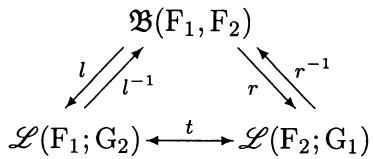
\includegraphics[keepaspectratio]{images/part003_fb3d81cd.jpg}}

where t is the isomorphism of transposition \(u \mapsto {}^{t}u\) . In view of the definition of the weak topologies on \(G_{1}\) and \(G_{2}\) , it is moreover immediate that when \(\mathfrak{B}(F_{1}, F_{2})\) , \(\mathcal{L}(F_{1}; G_{2})\) and \(\mathcal{L}(F_{2}; G_{1})\) are equipped with the topology of pointwise convergence, the isomorphisms in the preceding diagram are isomorphisms for the topological vector space structures.

Now let E, F be two Hausdorff locally convex spaces, \(E'\) , \(F'\) their respective duals; we denote by \(E_{\sigma}\) , \(F_{\sigma}\) the spaces E, F equipped with the weakened topologies \(\sigma(\mathrm{E}, \mathrm{E}')\) , \(\sigma(\mathrm{F}, \mathrm{F}')\) , and by \(E_{s}'\) , \(F_{s}'\) the spaces \(E'\) , \(F'\) equipped with the weak topologies \(\sigma(\mathrm{E}', \mathrm{E})\) , \(\sigma(\mathrm{F}', \mathrm{F})\) . Thus, the preceding remarks establish canonical isomorphisms between the three spaces \(\mathfrak{B}(\mathrm{E}_{\sigma}, \mathrm{F}_{s}')\) , \(\mathcal{L}(\mathrm{E}_{\sigma}; \mathrm{F}_{\sigma})\) and \(\mathcal{L}(\mathrm{F}_{s}'; \mathrm{E}_{s}')\) , and also between the three spaces \(\mathfrak{B}(\mathrm{E}_{\sigma}, \mathrm{F}_{\sigma})\) , \(\mathcal{L}(\mathrm{E}_{\sigma}; \mathrm{F}_{s}')\) and \(\mathcal{L}(\mathrm{F}_{\sigma}; \mathrm{E}_{s}')\) . One will observe that \(\mathfrak{B}(\mathrm{E}_{\sigma}, \mathrm{F}_{\sigma})\) is also equal to the space \(\mathfrak{B}(\mathrm{E}, \mathrm{F})\) of separately continuous bilinear forms on \(E \times F\) (E and F being equipped with their original topologies), since every continuous linear form on E (resp. F) is continuous on \(E_{\sigma}\) (resp. \(F_{\sigma}\) ) and conversely (TVS, II, §6, No.~1 and No.~2, Prop. 3).

Let \(\mathcal{B}(\mathrm{E},\mathrm{F})\) be the space of continuous bilinear forms on \(\mathbf{E}\times \mathbf{F}\) (E and F being equipped with their original topologies); then \(\mathcal{B}(\mathrm{E},\mathrm{F})\subset \mathfrak{B}(\mathrm{E},\mathrm{F})\) .

PROPOSITION 1. --- For a bilinear form \(\Phi \in \mathfrak{B}(\mathrm{E},\mathrm{F})\) to belong to \(\mathcal{B}(\mathrm{E},\mathrm{F})\) , it is necessary and sufficient that there exist a neighborhood of 0 in E whose image under \(^l\Phi\) is an equicontinuous subset of \(\mathbf{F}'\) .

For, to say that \(\Phi\) is continuous means that there exists a balanced convex neighborhood V (resp. W) of 0 in E (resp. F) such that \(|\Phi(x,y)| \leqslant 1\) for \(x \in V\) , \(y \in W\) ; this may be written \(|\langle^{l}\Phi(x), y \rangle| \leqslant 1\) for \(x \in V\) , \(y \in W\) , or also \(^{l}\Phi(V) \subset W^{\circ}\) ; whence the proposition, taking into account the fact that every equicontinuous subset of \(F'\) is contained in the polar of a neighborhood of 0 in F.

COROLLARY. --- If \(\Phi\) is a continuous bilinear form on \(\mathbf{E} \times \mathbf{F}\) , then \(^l\Phi\) is a continuous linear mapping of \(\mathbf{E}\) into the strong dual \(\mathbf{F}_b'\) of \(\mathbf{F}\) . If, moreover, \(\mathbf{E}\) and \(\mathbf{F}\) are normed spaces, then \(\|^l\Phi\| = \| \Phi \|\) .

The first assertion follows from Prop. 1 and the fact that every neighborhood of 0 in \(F_{b}^{\prime}\) absorbs every equicontinuous subset of \(F^{\prime}\) . If E and F are normed, then

\[
\begin{array}{c} \| \Phi \| = \sup _ {\| x \| \leqslant 1, \| y \| \leqslant 1} | \Phi (x, y) | = \sup _ {\| x \| \leqslant 1} \Big (\sup _ {\| y \| \leqslant 1} \big | \langle^ {l} \Phi (x), y \rangle \big | \Big) \\ = \sup _ {\| x \| \leqslant 1} \| ^ {l} \Phi (x) \| = \| ^ {l} \Phi \|, \end{array}
\]

whence the second assertion.

Interchanging the roles of E and F, one obtains results analogous to Prop. 1 and its corollary for the linear mappings \(r\Phi\) ; we leave to the reader the task of stating them.

\section{Some types of spaces having the property (GDF)}

We already know that every Fréchet space has the property (GDF) (TVS, I, §3, No.~3, Cor. 5 of Th. 1).

PROPOSITION 2. --- Let E be a vector space, \((\mathrm{F}_{\alpha})_{\alpha\in\mathrm{A}}\) a family of locally compact spaces having the property (GDF), and for each \(\alpha\in A\) let \(h_{\alpha}\) be a linear mapping of \(F_{\alpha}\) into E. If E is equipped with the finest locally convex topology that makes the \(h_{\alpha}\) continuous, then E has the property (GDF).

Let \(u\) be a linear mapping of \(\mathbf{E}\) into a Banach space \(\mathbf{B}\) , such that every limit in \(\mathbf{E} \times \mathbf{B}\) of every convergent sequence of points of the graph \(\Gamma\) of \(u\) also belongs to \(\Gamma\) . It suffices to show that, for every \(\alpha \in \mathbf{A}\) , \(u \circ h_{\alpha}\) is continuous on \(\mathrm{F}_{\alpha}\) (TVS, II, §4, No.~4, Prop. 5). Now, let \((x_n)\) be a sequence of elements of \(\mathrm{F}_{\alpha}\) having a limit \(a\) and such that the sequence \(\left(u(h_{\alpha}(x_n))\right)\) has a limit \(b \in \mathbf{B}\) . Since \(h_{\alpha}\) is continuous, \(h_{\alpha}(a)\) is a limit of the sequence \((h_{\alpha}(x_n))\) in \(\mathbf{E}\) ; therefore by hypothesis \(b = u(h_{\alpha}(a))\) and, since \(\mathrm{F}_{\alpha}\) has the property (GDF), \(u \circ h_{\alpha}\) is continuous.

COROLLARY. --- Every quotient space of a locally convex space having the property (GDF) has the property (GDF).

PROPOSITION 3. --- The strong dual of a reflexive Fréchet space has the property (GDF).

This is a consequence of Prop. 2 and the following lemma (or TVS, IV, §3, No.~4, Prop. 4):

Lemma. --- Let F be a Fréchet space, \(F'\) its strong dual, \(F''\) its bidual. If every subset of \(F''\) , bounded for \(\sigma(F'', F')\) , is contained in the closure (for \(\sigma(F'', F')\) ) of a bounded subset of F, then \(F'\) is the direct limit of a sequence of Banach spaces.

For, let \((\mathrm{V}_{n})\) be a decreasing fundamental sequence of convex, balanced and closed neighborhoods of 0 in F. For every integer n, let \(G_{n}\) be the linear subspace of \(F'\) generated by the polar \(V_{n}^{\circ}\) of \(V_{n}\) . In \(G_{n}\) , \(V_{n}^{\circ}\) is an absorbent convex set, therefore its gauge \(p_{n}\) is a norm on \(G_{n}\) ; moreover, \(V_{n}^{\circ}\) is a complete subset of the strong dual \(F'\) (TVS, III, §3, No.~8, Prop. 11); thus \(G_{n}\) , equipped with the norm \(p_{n}\) , is a Banach space (GT, III, §3, No.~5, Cor. 2 of Prop. 9). We are going to show that the strong topology on \(F'\) is the direct limit of these Banach space topologies on the \(G_{n}\) , or again that, for a strongly closed, balanced, convex subset U of \(F'\) to be a strong neighborhood of 0, it is necessary and sufficient that it absorb each of the \(V_{n}^{\circ}\) . It is obvious that this condition is necessary; to see that it is sufficient, it will suffice to prove that U contains a barrel of \(F'\) . Indeed, its polar \(U^{\circ}\) in \(F''\) will then be bounded for \(\sigma(\mathrm{F}''\mathrm{,}\mathrm{F}')\) , hence, by hypothesis, will be contained in the closure (for \(\sigma(\mathrm{F}''\mathrm{,}\mathrm{F}')\) ) of a bounded subset B of F, from which one can conclude that U (which is closed for \(\sigma(\mathrm{F}^{\prime},\mathrm{F}''\mathrm{)})\) ) contains the strong neighborhood \(B^{\circ}\) of 0 (TVS, II, §6, No.~3, Th. 1 and §8, No.~4).

By hypothesis, for every integer n there exists a number \(\lambda_{n}>0\) such that \(\lambda_{n}V_{n}^{\circ}\subset\frac{1}{2}U\) ; let \(A_{n}\) be the convex envelope of the union of the \(\lambda_{i}V_{i}^{\circ}\) for \(i\leqslant n\) . Then \(A_{n}\subset\frac{1}{2}U\) for every n; let W be the union of the \(A_{n}\) ; W is a convex, balanced, absorbent set contained in \(\frac{1}{2}U\) , and it will suffice to show that its strong closure (which is a barrel) is contained in U.

Thus, let \(x'\) be a point of \(F'\) not belonging to U. Since each of the \(V_n^\circ\) is compact for \(\sigma(F', F)\) , the same is true of the \(A_n\) (TVS, II, §2, No.~6, Prop. 15), and since \(x' \notin 2A_n\) , there exists an element \(x_n\) belonging to the polar of \(A_n\) in F such that \(\langle x', x_n \rangle = 2\) (TVS, II, §5, No.~3, Prop. 4). The sequence \((x_n)\) is bounded in F: for, every \(y' \in F'\) belongs to some \(V_k^\circ\) , consequently \(|\langle y', x_n \rangle| \leqslant \lambda_k^{-1}\) for \(n \geqslant k\) , whence our assertion (TVS, IV, §1, No.~1, Prop. 1). Let C be a bounded, balanced convex set in F containing all the \(x_n\) ; \(C^\circ\) is then a neighborhood of 0 in \(F'\) , and the polar \(C^{\circ\circ}\) of \(C^\circ\) in \(F''\) is compact for \(\sigma(F'', F')\) (TVS, III, §3, No.~4, Cor. 2 of Prop. 4 and No.~5, Prop. 7). Thus one sees that the sequence \((x_n)\) has a cluster point \(x''\) in \(F''\) for \(\sigma(F'', F')\) ; obviously \(\langle x', x'' \rangle = 2\) and, on the other hand, \(x''\) belongs to the polar of \(A_n\) in \(F''\) for every \(n\) , hence to the polar \(W^\circ\) of W in \(F''\) . From this, one concludes that \(x' \notin W^{\circ\circ}\) , hence is not in the closure of W for \(\sigma(F', F'')\) (TVS, II, §6, No.~3, Th. 1 and §8, No.~4), therefore a fortiori for the strong topology, which completes the proof.
% semantic-fragments: legacy-input-seam
\relax{}
\chapter*{Exercises}
\phantomsection
\addcontentsline{toc}{chapter}{Exercises}
\setcounter{exercisegroup}{1}
\edef\CurrentExerciseGroup{\arabic{exercisegroup}}
\section*{\texorpdfstring{\S\CurrentExerciseGroup}{Section \CurrentExerciseGroup}}
\phantomsection
\addcontentsline{toc}{section}{\texorpdfstring{Exercises for \S\CurrentExerciseGroup}{Exercises for Section \CurrentExerciseGroup}}

\begin{enumerate}
\def\labelenumi{\arabic{enumi})}
\item
  Consider the locally compact spaces T, T' identical to the interval {[}0, 1{]}, and the measures \(\mu, \mu'\) on T and T', respectively, identical to the Lebesgue measure. Let F be a Hilbert space admitting a countable orthonormal basis, arranged in a double sequence \((\mathbf{e}_{mn})\) ; let F' = F be its dual. Set \(\mathbf{u}_m(t) = \mathbf{e}_{mn}\) for \((n-1)2^{-m} \leqslant t < n2^{-m}\) and \(1 \leqslant n \leqslant 2^m\) ; set \(\mathbf{f}(t, t') = 2^m \mathbf{u}_m(t)\) for \(2^{-m} < t' \leqslant 2^{-m+1}\) , and finally \(\mathbf{f}(t, 0) = 0\) and \(\mathbf{f}(1, t') = 0\) . Show that \(\mathbf{f}\) is scalarly integrable for the product measure \(\mu \otimes \mu'\) , but that the function \(t' \mapsto \mathbf{f}(t, t')\) is not scalarly \(\mu'\) -integrable for any \(t \in T\) .
\item
  Let \(\mathrm{T}, \mathrm{X}, \mathrm{Y}\) be three locally compact spaces, with \(\mathrm{Y}\) having a countable base. Let \(\mu\) be a measure \(\geqslant 0\) on \(\mathrm{T}\) , \(t \mapsto \lambda_t (t \in \mathrm{T})\) a \(\mu\) -adequate \(^1\) family of measures \(\geqslant 0\) on \(\mathrm{X}\) , and set \(\nu = \int \lambda_t d\mu(t)\) . Let \(x \mapsto \rho_x (x \in \mathrm{X})\) be a \(\nu\) -adequate family of measures \(\geqslant 0\) on \(\mathrm{Y}\) . Suppose, moreover, that one of the following two conditions is satisfied: a) \(\mathrm{X}\) is countable at infinity;
\end{enumerate}

\begin{enumerate}
\def\labelenumi{\alph{enumi})}
\setcounter{enumi}{1}
\tightlist
\item
  \(\nu\) is bounded.
\end{enumerate}

Under these conditions, show that there exists a locally \(\mu\) -negligible set \(N'\) such that, for every \(t \notin N'\) , the family \(x \mapsto \rho_x\) is \(\lambda_t\) -adequate; moreover, the family \(t \mapsto \int \rho_x d\lambda_t(x)\) , defined for \(t \notin N'\) , is \(\mu\) -adequate, and

\[
\int d \mu (t) \int \rho_ {x} d \lambda_ {t} (x) = \int \rho_ {x} d \nu (x).
\]

(To prove that \(x \mapsto \rho_x\) is scalarly \(\lambda_t\) -integrable locally almost everywhere, make use of Lemma 1 of §3, No.~1, using, in case \(b\) ), the fact that \(\lambda_t\) is bounded locally almost everywhere; same method for seeing that \(t \mapsto \int \rho_x d\lambda_t(x)\) is scalarly \(\mu\) -integrable; use also Prop. 13 of No.~5.)

\begin{enumerate}
\def\labelenumi{\arabic{enumi})}
\setcounter{enumi}{2}
\tightlist
\item
  Let S, T, Y be three locally compact spaces, countable at infinity, with Y having a countable base. Let \(\rho\) (resp. \(\sigma\) ) be a positive measure on S (resp. T), \(\nu = \rho \otimes \sigma\) , and let \((\lambda_{s,t})_{(s,t) \in \mathbb{S} \times \mathbb{T}}\) be a \(\nu\) -adequate \(^{1}\) family of positive measures on Y. Then, there exists a \(\rho\) -negligible set N such that, for every \(s \notin N\) , the family \((\lambda_{s,t})_{t \in \mathbb{T}}\) is \(\sigma\) -adequate; the family \(s \mapsto \int \lambda_{s,t} d\sigma(t)\) (defined almost everywhere) is \(\rho\) -adequate, and
\end{enumerate}

\[
\iint \lambda_ {s, t} d \rho (s) d \sigma (t) = \int d \rho (s) \int \lambda_ {s, t} d \sigma (t).
\]

(Apply Exer. 2 to the space \(\mathrm{X} = \mathrm{S} \times \mathrm{T}\) , on noting that \(\nu = \int (\varepsilon_s \otimes \sigma) d\rho(s)\) .)

\begin{enumerate}
\def\labelenumi{\arabic{enumi})}
\setcounter{enumi}{3}
\tightlist
\item
  Let \(\mathrm{T}, \mathrm{X}, \mathrm{Y}\) be three locally compact spaces, with \(\mathrm{X}\) being countable at infinity. Let \(\mu\) be a positive measure on \(\mathrm{T}\) , \((\lambda_t)_{t \in \mathrm{T}}\) a \(\mu\) -adequate family of positive measures on \(\mathrm{X}\) , and \(\nu = \int \lambda_t d\mu(t)\) . Assume that one of the following two conditions holds:
\end{enumerate}

\begin{enumerate}
\def\labelenumi{\alph{enumi})}
\item
  Y has a countable base;
\item
  the measure \(\nu\) is bounded.
\end{enumerate}

Under these conditions, if \(\pi\) is a \(\nu\) -proper mapping of X into Y, then the set of \(t \in \mathbf{T}\) such that \(\pi\) is not \(\lambda_t\) -proper is locally \(\mu\) -negligible; moreover, the family \((\pi(\lambda_t))_{t \in \mathbf{T}}\) of positive measures on Y (defined locally almost everywhere in T) is \(\mu\) -adequate, and

\[
\pi \left(\int \lambda_ {t} d \mu (t)\right) = \int \pi (\lambda_ {t}) d \mu (t).
\]

(In case \(a\) ), apply Exer. 2 to \(\rho_x = \varepsilon_{\pi(x)}\) . In case \(b\) ), note that \(\lambda_t\) is bounded locally almost everywhere, and reduce to showing that the mapping \(t \mapsto \pi(\lambda_t)\) is vaguely \(\mu\) -measurable (cf.~Ch. V, §3, No.~2, Prop. 4). Given a number \(\varepsilon > 0\) and a compact subset \(K\) of \(T\) , observe first that there exists in \(X\) an increasing sequence \((F_m)\) of compact sets such that the restriction of \(\pi\) to each \(F_m\) is continuous and such that, on setting \(N_m = X - F_m\) , \(\nu(N_m) \leqslant \varepsilon/4^m\) . Let \(A_m\) be the set of \(t \in K\) such that \(N_m\) is not \(\lambda_t\) -integrable or such that \(\lambda_t(N_m) > 1/2^m\) ; if \(A\) is the union of the \(A_m\) , \(\mu(A) \leqslant \varepsilon/2\) . Let \(K_1\) be a compact subset of \(K - A\) such that \(\mu(K - K_1) \leqslant \varepsilon\) and such that, for every function \(g \in \mathcal{H}(X)\) , the restriction of \(t \mapsto \int g(x) d\lambda_t(x)\) to \(K_1\) is continuous. Using Urysohn's theorem, show that for every function \(f \in \mathcal{H}(Y)\) , the restriction to \(K_1\) of \(t \mapsto \int f(\pi(x)) d\lambda_t(x)\) is the uniform limit of continuous functions.)

*5) For every \(t \in \mathbf{R}\) let \(\mathbf{f}(t)\) be the continuous function \(x \mapsto \exp(-2\pi itx)\) , which is an element of the space \(\mathcal{C} = \mathcal{C}_{\mathbf{C}}(\mathbf{R})\) of continuous complex functions on \(\mathbf{R}\) . The space \(\mathcal{C}\) is in duality with the space \(\mathcal{C}' = \mathcal{C}'_{\mathbf{C}}(\mathbf{R})\) of complex measures on \(\mathbf{R}\) with compact support; the space \(\mathcal{K} = \mathcal{K}_{\mathbf{C}}(\mathbf{R})\) of continuous complex functions with compact support may be canonically identified with a subspace of \(\mathcal{C}'\) , by identifying a function \(\varphi \in \mathcal{K}\) with the measure having density \(\varphi\) with respect to Lebesgue measure. One denotes by \(\mathcal{D}\) the subspace of \(\mathcal{K}\) formed by the indefinitely differentiable complex functions with compact support. Show that, when \(\mathcal{C}\) is equipped with the topology \(\sigma(\mathcal{C},\mathcal{C}')\) or with the topology \(\sigma(\mathcal{C},\mathcal{K})\) , \(\mathbf{f}\) is not scalarly integrable for the Lebesgue measure \(\mu\) ; however, for the topology \(\sigma(\mathcal{C},\mathcal{D})\) , \(\mathbf{f}\) is scalarly \(\mu\) -integrable and \(\int f d\mu\) is the measure \(\varepsilon_0\) ; prove that in this case, the conditions of Prop. 7 are verified.*

\begin{enumerate}
\def\labelenumi{\arabic{enumi})}
\setcounter{enumi}{5}
\item
  Let F be a distinguished (TVS, IV, §2, Exer. 4 b)) Fréchet space, F' its dual. Show that if f is a scalarly essentially integrable mapping of T into F, then \(\int f d\mu\) belongs to the bidual F'\,' of F. (Embed F in F'\,'; apply Th. 1, as well as Prop. 2 and the Lemma of the Appendix.)
\item
  \begin{enumerate}
  \def\labelenumii{\alph{enumii})}
  \tightlist
  \item
    Let \(\mathbf{F} = \overline{\mathcal{K}(\mathbf{N})}\) be the Banach space of sequences of real numbers tending to 0, \(\mathbf{F}' = \mathbf{L}^1 (\mathbf{N})\) its dual (TVS, IV, §1, Exer. 1). Let \(\mathbf{f} = (f_n)\) be the mapping of \(\mathrm{I} = [0,1]\) into \(\mathbf{F}\) such that \(f_{n}(t) = n\varphi_{\mathrm{I}_{n}}(t)\) , where \(\mathrm{I}_n = [0,1 / n]\) . Show that \(\mathbf{f}\) is scalarly integrable for the Lebesgue measure \(\mu\) on \(\mathrm{I}\) , but that \(\int \mathbf{f}d\mu\) is an element of \(\mathbf{F}''\) not in \(\mathbf{F}\) .
  \end{enumerate}
\end{enumerate}

\begin{enumerate}
\def\labelenumi{\alph{enumi})}
\setcounter{enumi}{1}
\item
  Let \(\mathbf{g}\) be the mapping of \(J = [-1, +1]\) into \(F\) defined by the conditions \(\mathbf{g}(t) = \mathbf{f}(t)\) for \(t \geqslant 0\) , \(\mathbf{g}(t) = -\mathbf{f}(-t)\) for \(t \leqslant 0\) . Then \(\mathbf{g}\) is scalarly integrable for Lebesgue measure on \(J\) , and \(\int \mathbf{g} d\mu \in F\) , but there exist functions \(h \in \mathcal{L}^{\infty}\) such that \(\int h\mathbf{g} d\mu \notin F\) .
\item
  Deduce from \(a\) ) a new proof of the fact that the topological vector space \(F\) is not isomorphic to the dual of a normed space (TVS, IV, §2, Exer. 22 c)).
\end{enumerate}

\begin{enumerate}
\def\labelenumi{\arabic{enumi})}
\setcounter{enumi}{7}
\tightlist
\item
  Let \(\mathbf{F}\) be a Hausdorff locally convex space, \(\mathbf{f}\) a scalarly locally integrable mapping of \(\mathbf{T}\) into \(\mathbf{F}\) such that, for every compact subset \(\mathbf{K}\) of \(\mathbf{T}\) , \(\int_{\mathbf{K}} \mathbf{f} d\mu \in \mathbf{F}\) .
\end{enumerate}

\begin{enumerate}
\def\labelenumi{\alph{enumi})}
\item
  Show that if \(\mathbf{f}\) is scalarly essentially integrable, and if \(\mathrm{F}\) is semi-reflexive (or if merely every Cauchy sequence for \(\sigma (\mathrm{F},\mathrm{F}^{\prime})\) converges in \(\mathrm{F}\) for this topology, when \(\mathrm{T}\) is countable at infinity), then \(\int g\mathbf{f}d\mu \in \mathrm{F}\) for every function \(g\in \mathcal{L}^{\infty}\) .
\item
  Show that if F is quasi-complete and if, for every continuous semi-norm q on F, one has \(\int^{\bullet} q(\mathbf{f}(t)) d\mu(t) < +\infty\) , then f is scalarly essentially integrable and \(\int g\mathbf{f} d\mu \in F\) for every function \(g \in L^{\infty}\) .
\end{enumerate}

(In both cases, consider the increasing directed set of compact subsets of T.)

\begin{enumerate}
\def\labelenumi{\arabic{enumi})}
\setcounter{enumi}{8}
\item
  Let G,H be two Hausdorff locally convex spaces, U a mapping of T into \(F = \mathcal{L}_{s}(G;H)\) . Assume that G is barreled, H is quasi-complete, U is \(\mu\) -measurable and \(U(K)\) is bounded for every compact subset K of T; assume, moreover, that for every continuous semi-norm q on H and every \(x \in G\) , \(\int^{\bullet} q(U(t) \cdot x) d\mu(t) < +\infty\) . Under these conditions, show that U is scalarly essentially \(\mu\) -integrable and that \(\int U(t) d\mu(t) \in F\) (make use of Exercise 8 b)).
\item
  Let \(G, H\) be two Fréchet spaces, \(G_0\) (resp. \(H_0\) ) a dense subset of \(G\) (resp. \(H\) ), and \(t \mapsto \Phi_t\) a mapping of \(T\) into the space \(F = \mathcal{B}(G, H)\) of continuous bilinear forms on \(G \times H\) , equipped with the topology of pointwise convergence. Assume that: \(1^\circ\) for every pair \((a, b) \in G_0 \times H_0\) , \(t \mapsto \Phi_t(a, b)\) is essentially \(\mu\) -integrable; \(2^\circ\) if, for every pair of bounded subsets \(A \subset G\) , \(B \subset H\) , one sets \(q_{A,B}(\Phi) = \sup_{(x, y) \in A \times B} |\Phi(x, y)|\) for
\end{enumerate}

every \(\Phi \in \mathcal{B}(\mathrm{G},\mathrm{H})\) , then \(\int^{*}q_{\mathrm{A},\mathrm{B}}(\Phi_t)d\mu (t) < + \infty\) . Under these conditions, show that \(t\mapsto \Phi_t\) is scalarly essentially \(\mu\) -integrable and \(\int \Phi_t d\mu (t)\in \mathrm{F}\) (using Lebesgue's theorem, reduce to applying Cor. 1 of Th. 1). Special case where \(\mathrm{H} = \mathbf{R}\) .

\begin{enumerate}
\def\labelenumi{\arabic{enumi})}
\setcounter{enumi}{10}
\item
  Let \(\mu\) be Lebesgue measure on \(T = [0,1]\) , \(F\) a Hilbert space having a countable orthonormal basis \((\mathbf{e}_n)\) . Let \(\mathbf{f}\) be the mapping of \(T\) into \(F\) such that \(\mathbf{f}(0) = 0\) and \(\mathbf{f}(t) = 2^n \mathbf{e}_n / n\) on the interval \([2^{-n-1}, 2^{-n}]\) ( \(n \geqslant 0\) ). Show that \(\mathbf{f}\) is \(\mu\) -measurable, scalarly \(\mu\) -integrable, and that \(\int \mathbf{f} d\mu \in F\) , but that \(\int^* |\mathbf{f}| d\mu = +\infty\) .
\item
  Let \(\mu\) be Lebesgue measure on \(T = [0,1]\) , and let \(F\) be a Hilbert space having an orthonormal basis \((\mathbf{e}_t)_{t \in T}\) equipotent to \(T\) .
\end{enumerate}

\begin{enumerate}
\def\labelenumi{\alph{enumi})}
\item
  Let \(\mathbf{f}\) be the mapping \(t \mapsto \mathbf{e}_t\) of \(\mathrm{T}\) into \(\mathrm{F}\) . Show that \(\mathbf{f}\) is scalarly \(\mu\) -negligible, but is not \(\mu\) -measurable when \(\mathrm{F}\) is equipped with the weak topology \(\sigma(\mathrm{F}, \mathrm{F}')\) (nor, a fortiori, when \(\mathrm{F}\) is equipped with its original topology).
\item
  Let A be a non-measurable set in T (Ch. IV, §4, Exer. 8); show that the function \(\mathbf{g} = \mathbf{f}\varphi_{\mathrm{A}}\) is scalarly \(\mu\) -negligible, but that the numerical function \(|\mathbf{g}|\) is not \(\mu\) -measurable.
\end{enumerate}

\begin{enumerate}
\def\labelenumi{\arabic{enumi})}
\setcounter{enumi}{12}
\item
  Let F be a Hausdorff locally convex space, \(F'\) its dual, q a lower semi-continuous semi-norm on F. Show that if f is a mapping of T into F, \(\mu\) -measurable for the topology \(\sigma(\mathrm{F},\mathrm{F}')\) , then the numerical function \(q \circ f\) is \(\mu\) -measurable.
\item
  Let \(\mu\) be Lebesgue measure on T = {[}0,1{]}; denote by F the vector space over R of \(\mu\) -measurable finite numerical functions on T, equipped with the topology of pointwise convergence, which makes it a Hausdorff locally convex space.
\end{enumerate}

\begin{enumerate}
\def\labelenumi{\alph{enumi})}
\item
  Show that there exists in F a countable dense subset (consider a dense sequence in the Banach space \(\mathcal{C}(T)\) of continuous numerical functions on T).
\item
  For every \(t \in T\) , let \(\mathbf{f}(t)\) be the element of the dual \(F'\) of F defined by \(\langle\mathbf{f}(t), z\rangle = z(t)\) for all \(t \in T\) . Show that, when \(F'\) is equipped with the topology \(\sigma(\mathrm{F}', \mathrm{F})\) , f is scalarly \(\mu\) -measurable but is not \(\mu\) -measurable (cf.~Prop. 13).
\end{enumerate}

\begin{enumerate}
\def\labelenumi{\arabic{enumi})}
\setcounter{enumi}{14}
\item
  Let F be a metrizable locally convex space, f a scalarly \(\mu\) -measurable mapping of T into F such that, for every compact subset K of T, there exists a countable subset H of F such that \(\mathbf{f}(t) \in \overline{\mathbf{H}}\) for almost every \(t \in K\) ; show that under these conditions, f is \(\mu\) -measurable for the original topology of F. (Embed F in a countable product of normed spaces, after having reduced to the case that F is separable.)
\item
  Let \(\mathbf{F}\) be a Banach space, \(\mathbf{F}'\) its dual. For every \(p\) such that \(1 \leqslant p \leqslant +\infty\) , denote by \(\Lambda_{\mathbf{F}'}^p(\mathrm{T},\mu)\) (or simply by \(\Lambda_{\mathbf{F}'}^p\) ) the set of mappings \(\mathbf{f}\) of \(\mathrm{T}\) into \(\mathbf{F}'\) such that, for every \(\mathbf{z} \in \mathbf{F}\) , the numerical function \(\langle \mathbf{z},\mathbf{f}\rangle\) belongs to \(\mathcal{L}^p(\mathrm{T},\mu)\) . One has \(\Lambda_{\mathbf{F}'}^p \supset \mathcal{L}_{\mathbf{F}'}^p\) , and \(\Lambda_{\mathbf{F}'}^1\) is the space of scalarly essentially \(\mu\) -integrable functions with values in \(\mathbf{F}'\) ( \(\mathbf{F}'\) being equipped with \(\sigma(\mathbf{F}',\mathbf{F})\) ). One knows that, denoting by \(\theta(\mathbf{z})\) the class of \(\langle \mathbf{z},\mathbf{f}\rangle\) in \(\mathrm{L}^p(\mu)\) , the mapping \(\mathbf{z} \mapsto \theta(\mathbf{z})\) is continuous (No.~4, Lemma 2); let \(M_p(\mathbf{f})\) be its norm; this is a semi-norm on the space \(\Lambda_{\mathbf{F}'}^p\) . In order that \(M_p(\mathbf{f}) = 0\) , it is necessary and sufficient that \(\mathbf{f}\) be scalarly locally negligible.
\end{enumerate}

\begin{enumerate}
\def\labelenumi{\alph{enumi})}
\item
  In order that \(\mathbf{f} \in \Lambda_{\mathbf{F}'}^p\) , it is necessary and sufficient that for every numerical function \(g \in \mathcal{L}^q\) , the function \(g\mathbf{f}\) be scalarly essentially \(\mu\) -integrable; one then has \(\mathrm{M}_1(g\mathbf{f}) \leqslant \mathrm{M}_p(\mathbf{f})\mathrm{N}_q(g)\) .
\item
  In the space \(\Lambda_{\mathbf{F}'}^1\) , show that the semi-norm \(\mathbf{M}_1\) is equivalent to the semi-norm \(\mathrm{M}_1'(\mathbf{f}) = \sup |\int_{\mathbf{A}} \mathbf{f} d\mu|\) , where A runs over the set of measurable subsets of T; more precisely, \(\mathrm{M}_1' \leqslant \mathrm{M}_1 \leqslant 2\mathrm{M}_1'\) . Deduce from this that \(\mathrm{M}_p\) is a semi-norm equivalent to \(\mathrm{M}_p'(\mathbf{f}) = \sup_{\mathrm{N}_q(g) \leqslant 1} \mathrm{M}_1'(g\mathbf{f})\) .
\item
  Take for F a Hilbert space having a countable orthonormal basis, and for \(\mu\) the Lebesgue measure on \(T = [0,1]\) . Show that there exists a mapping of T into F, not integrable but scalarly integrable, that is the limit for the semi-norm \(M_1\) of a sequence of measurable step functions (cf.~Exer. 11); from this, deduce that on the space \(\mathcal{L}_{\mathrm{F}}^1\) , of \(\mu\) -integrable functions, the topology defined by the semi-norm \(M_1\) is strictly coarser than that defined by \(N_1\) . Analogous result for the semi-norms \(M_p\) and \(N sub p\) , for \(1 \leqslant p < +\infty\) .
\end{enumerate}

\(d\) ) Show that on the space \(\mathcal{L}_{\mathrm{F}^{\prime}}^{\infty}\) , \(\mathrm{M}_{\infty} = \mathrm{N}_{\infty}\)

\begin{enumerate}
\def\labelenumi{\alph{enumi})}
\setcounter{enumi}{4}
\tightlist
\item
  Take for F a Hilbert space having a countable orthonormal basis, arranged in a double sequence \((\mathbf{e}_{mn})\) . Let \(\mu\) be Lebesgue measure on \(T = [0,1]\) . Let \(\mathbf{u}_m\) be the mapping of T into F such that \(\mathbf{u}_m(t) = \mathbf{e}_{mn}\) for \((n - 1)2^{-m} \leqslant t < n2^{-m}\) and for \(1 \leqslant n \leqslant 2^m\) , and \(\mathbf{u}_m(1) = 0\) ; set \(\mathbf{f}_n = \sum_{i=0}^{n} \mathbf{u}_i\) . Show that, for \(1 \leqslant p < +\infty\) , \((\mathbf{f}_n)\) is a Cauchy sequence in \(\Lambda_{\mathrm{F}'}^p\) but does not converge to any function in \(\Lambda_{\mathrm{F}'}^p\) .
\end{enumerate}

\begin{enumerate}
\def\labelenumi{\alph{enumi})}
\setcounter{enumi}{5}
\item
  Let \((\mathbf{f}_{n})\) be a Cauchy sequence in the space \(\Lambda_{F'}^{p}\) ( \(1 \leqslant p \leqslant +\infty\) ); assume that there exists a mapping f of T into \(F'\) such that, for every \(z \in F\) , the sequence of functions \(\langle z, f_{n} \rangle\) converges in measure to \(\langle z, f \rangle\) (Ch. IV, §5, No.~11). Show that \(f \in \Lambda_{F'}^{p}\) and that the sequence \((\mathbf{f}_{n})\) has limit f in \(\Lambda_{F'}^{p}\) .
\item
  Take for F the Banach space \(\mathrm{L}^{1}(\mathbf{N})\) of absolutely convergent series; its dual is \(\mathbf{F}^{\prime} = \mathrm{L}^{\infty}(\mathbf{N})\) (TVS, IV, §1, Exer. 1). Let \(\mu\) be Lebesgue measure on T = {[}0,1{]}. Let f be the mapping of T into \(F^{\prime}\) such that \(\mathbf{f}(0) = 0\) and, for \(2^{-n-1} < t \leqslant 2^{-n}\) , \(\mathbf{f}(t)\) is the sequence all of whose terms are zero, except for the term of index n, equal to \(2^{n/p}\) for \(1 \leqslant p < +\infty\) . Show that f is measurable for the strong topology on \(F^{\prime}\) , and belongs to \(\Lambda_{\mathrm{F}'}^p\) , but that there does not exist any sequence \((\mathbf{f}_n)\) of step functions that tends to \(\mathbf{f}\) in the space \(\Lambda_{\mathrm{F}'}^p\) .
\end{enumerate}

¶ 17) Let \(\mu\) be Lebesgue measure on \(T = [0,1]\) , \(F\) the Banach space \(L^1(\mathbf{N})\) , \(F' = L^\infty(\mathbf{N})\) its dual. For every \(t \in [0,1[\) , let \(t = \sum_{n=0}^\infty \xi_n 2^{-n}\) be the dyadic expansion of \(t\) ; denote by \(f(t)\) the sequence \((\xi_n) \in F'\) , and set \(f(1) = 0\) .

\begin{enumerate}
\def\labelenumi{\alph{enumi})}
\item
  Show that, for \(1 \leqslant p \leqslant +\infty\) , the function \(\mathbf{f}\) belongs to the space \(\Lambda_{\mathrm{F}'}^p\) (cf.~Exer. 16).
\item
  Show that \(\mathbf{f}\) is measurable for the topology \(\sigma(\mathrm{F}',\mathrm{F})\) and that, for this topology, there exists a sequence of step functions that converges almost everywhere to \(\mathbf{f}\) .
\item
  Show that \(\mathbf{f}\) is not measurable for the strong topology on \(\mathbf{F}'\) (observe that \(|\mathbf{f}(t) - \mathbf{f}(t')| = 1\) if \(0 \leqslant t < t' < 1\) ).
\item
  Show that, in the space \(\Lambda_{\mathrm{F}'}^p\) ( \(1 \leqslant p < +\infty\) ), \(\mathbf{f}\) is not the limit of a sequence of step functions. (Reduce to considering only step functions that are linear combinations (with coefficients in \(\mathbf{F}'\) ) of characteristic functions of intervals whose endpoints are of the form \(k/2^n\) ; if \(\mathbf{g}\) is such a step function, show that, in the notations of Exer. 16 b), \(\mathrm{M}_1'(\mathbf{f} - \mathbf{g}) \geqslant 1/4\) .)
\item
  Show that there does not exist any mapping \(\mathbf{h}\) of \(\mathrm{T}\) into \(\mathrm{F}'\) , measurable for the strong topology, such that \(\mathbf{f} - \mathbf{h}\) is scalarly negligible. (Observe that, for such a mapping, one would necessarily have \(\mathrm{N}_{\infty}(\mathbf{h}) \leqslant 1\) ; then obtain a contradiction with the result of \(d\) .)
\end{enumerate}

\begin{enumerate}
\def\labelenumi{\arabic{enumi})}
\setcounter{enumi}{17}
\tightlist
\item
  Show that Prop. 8 continues to hold when the condition that \(\mathbf{f}\) be \(\mu\) -measurable (for the original topology of \(\mathbf{F}\) ) is replaced by the condition that \(\mathbf{f}\) be \(\mu\) -measurable for the weakened topology \(\sigma(\mathrm{F},\mathrm{F}')\) . (Make use of Exer. 19 c) of Ch. IV, §4.)
\end{enumerate}

¶ 19) Let f be a scalarly essentially μ-integrable mapping of T into F. For every \(z' \in F'\) , denote by \(u_{\mathbf{f}}(\mathbf{z}')\) the class in \(L^{1}(\mu)\) of the function \(\langle f, z' \rangle\) . We shall say that f is scalarly well integrable if, for every function \(g \in L^{\infty}(\mu)\) , \(\int g f d\mu \in F\) .

\begin{enumerate}
\def\labelenumi{\alph{enumi})}
\item
  For \(\mathbf{f}\) to be scalarly well integrable, it is necessary and sufficient that \(u_{\mathbf{f}}\) be continuous for the topologies \(\sigma(\mathrm{F}',\mathrm{F})\) and \(\sigma(\mathrm{L}^1,\mathrm{L}^\infty)\) . When this is so, the image under \(u_{\mathbf{f}}\) of every equicontinuous subset of \(\mathrm{F}'\) is a relatively weakly compact subset of \(\mathrm{L}^1\) . In particular: \(\alpha\) for every equicontinuous subset \(\mathrm{H}'\) of \(\mathrm{F}'\) and every \(\varepsilon >0\) , there exists a compact subset \(\mathrm{L}\) of \(\mathrm{T}\) such that \(\int_{\mathrm{T}-\mathrm{L}}|\langle\mathbf{f},\mathbf{z}'\rangle|d\mu\leqslant\varepsilon\) for all \(\mathbf{z}'\in\mathrm{H}'\) ; \(\beta\) for every equicontinuous subset \(\mathrm{H}'\) of \(\mathrm{F}'\) and every \(\varepsilon>0\) , there exists an \(\eta>0\) such that, for every open set \(\mathrm{U}\subset\mathrm{T}\) of measure \(\mu(\mathrm{U})\leqslant\eta\) , one has \(\int_{\mathrm{U}}|\langle\mathbf{f},\mathbf{z}'\rangle|d\mu\leqslant\varepsilon\) for all \(\mathbf{z}'\in\mathrm{H}'\) (Ch. V, §5, Exer. 15).
\item
  Assume that the conditions \(\alpha\) and \(\beta\) of \(a\) ) are verified and, moreover, that there exists a subspace \(\mathrm{H} \subset \mathrm{L}^{\infty}\) , dense for the topology \(\sigma(\mathrm{L}^{\infty}, \mathrm{L}^{1})\) , such that for every function \(g \in \mathcal{L}^{\infty}\) whose class is in \(\mathrm{H}\) , one has \(\int g\mathbf{f}d\mu \in \mathrm{F}\) . Show that under these conditions, if in addition \(\mathrm{F}\) is assumed to be quasi-complete, then \(\mathbf{f}\) is scalarly well integrable. (First reduce to the case that \(\mathrm{F}\) is complete (for its original topology), and observe that \(\dot{g} \mapsto \int g\mathbf{f}d\mu\) is a continuous linear mapping of \(\mathrm{L}^{\infty}\) into \(\mathrm{F}'*\) , when \(\mathrm{L}^{\infty}\) is equipped with the topology \(\tau(\mathrm{L}^{\infty}, \mathrm{L}^{1})\) and \(\mathrm{F}'*\) with the topology of uniform convergence on the equicontinuous subsets of \(\mathrm{F}'\) .)
\item
  Suppose that \(\mathbf{f}\) is scalarly well integrable. Show that for every Cauchy sequence \((\mathbf{z}_n')\) for the topology \(\sigma(\mathrm{F}',\mathrm{F})\) , the sequence \((u_{\mathbf{f}}(\mathbf{z}_n'))\) is strongly convergent in \(\mathrm{L}^1\) (use Exer. 25 c) of Ch. IV, §5 and Exer. 16 b) of Ch. V, §5). From this, deduce that if A is the image of the unit ball of \(\mathrm{L}^{\infty}\) under the mapping \(\dot{g} \mapsto \int g\mathbf{f}d\mu\) , then every Cauchy sequence \((\mathbf{z}_n')\) for the topology \(\sigma(\mathrm{F}',\mathrm{F})\) is a Cauchy sequence for the topology of uniform convergence in A.
\end{enumerate}

\(d)\) Deduce from \(c)\) that if \(\mathbf{f}\) is scalarly well integrable, then the image under \(u_{\mathbf{f}}\) of every subset of \(\mathrm{F}'\) that is equicontinuous and metrizable for \(\sigma (\mathrm{F}',\mathrm{F})\) , is relatively strongly compact in \(L^{1}\) . In particular, if F is the dual \(G'\) of a Hausdorff locally convex space G, if F is equipped with a topology compatible with the duality between F and G, and if there exists in \(G'\) a countable strongly dense subset, then the image under \(u_{f}\) of every bounded subset of \(F' = G\) is relatively strongly compact in \(L^{1}\) (embed G in its bidual).

\begin{enumerate}
\def\labelenumi{\arabic{enumi})}
\setcounter{enumi}{19}
\tightlist
\item
  Let F be a Hausdorff locally convex space, \(F'\) its dual, \(S'\) the set of subsets \(A' \subset F'\) such that every sequence of points of \(A'\) has a subsequence convergent for \(\sigma(\mathrm{F}',\mathrm{F})\) . Show that, for a bounded subset A of F, the following conditions are equivalent: \(\alpha\) A is precompact for the \(S'\) -topology; \(\beta\) every sequence convergent for \(\sigma(\mathrm{F}',\mathrm{F})\) converges uniformly on A. (Let S be the set formed by the finite subsets of F and of A; observe that \(\beta\) ) implies that every set \(A' \in S'\) is precompact for the S-topology, using Exer. 6 of GT, II, §4. Then apply Exer. 4 of TVS, IV, §1.)
\end{enumerate}

¶ 21) Let f be a scalarly well integrable mapping of T into a quasi-complete Hausdorff locally convex space F.

\begin{enumerate}
\def\labelenumi{\alph{enumi})}
\item
  Show that the image under \(\dot{g} \mapsto \int g\mathbf{f}  d\mu\) of the unit ball of \(\mathrm{L}^{\infty}\) is a relatively compact subset of \(\mathbf{F}\) for the original topology, in each of the following cases: \(1^{\circ}\) there exists a countable dense subset of \(\mathbf{F}\) ; \(2^{\circ}\) \(\mathbf{F}\) is the dual \(\mathbf{G}'\) of a space \(\mathbf{G}\) that is either metrizable or is the strict direct limit of a sequence of metrizable spaces, and \(\mathbf{F}\) is equipped with the topology \(\tau (\mathbf{G}',\mathbf{G})\) . (Make use of Exer. 19 c) and Exer. 20; in case \(2^{\circ}\) , use Šmulian's theorem (TVS, IV, §5, Exer. 2 c)).
\item
  Show that the conclusion of a) remains valid when, with no new hypothesis on F, one assumes f to be measurable. (Embedding F in a product of Banach spaces, reduce to the case that F is a Banach space; then, using Exer. 19 a), reduce to the case that T is compact; then apply case \(1^{\circ}\) of a).
\end{enumerate}

\begin{enumerate}
\def\labelenumi{\arabic{enumi})}
\setcounter{enumi}{21}
\tightlist
\item
  In a Hausdorff locally convex space \(\mathbf{F}\) , let \((\mathbf{z}_{\alpha})_{\alpha \in \mathbf{A}}\) be a family such that the mapping \(\alpha \mapsto \mathbf{z}_{\alpha}\) is scalarly well integrable (Exer. 19) when \(\mathbf{A}\) is equipped with the measure defined by mass \(+1\) at each point.
\end{enumerate}

\begin{enumerate}
\def\labelenumi{\alph{enumi})}
\item
  Show that the family \((\mathbf{z}_{\alpha})\) is summable for every topology T compatible with the duality between F and \(F'\) (make use of Exer. 19 a)). Converse when F is quasi-complete for T.
\item
  Suppose that \(F = G'\) , \(F' = G\) , where G is a Hausdorff locally convex space such that there exists in \(G'\) a countable strongly dense subset. Show that \((\mathbf{z}_{\alpha})\) is then summable for the strong topology on \(G'\) (which is not necessarily compatible with the duality between \(G'\) and G (cf.~Exer. 19d)). Show that this result does not extend to the case that \(G = L^{1}(\mathbf{N})\) , \(G' = L^{\infty}(\mathbf{N})\) .
\end{enumerate}

\begin{enumerate}
\def\labelenumi{\arabic{enumi})}
\setcounter{enumi}{22}
\tightlist
\item
  Let \(\mu\) be a positive measure on \(T\) , carried by a countable union of compact sets.
\end{enumerate}

\begin{enumerate}
\def\labelenumi{\alph{enumi})}
\tightlist
\item
  Let H be a set of \(\mu\) -measurable numerical functions, such that for every \(t \in \mathbf{T}\) , \(\sup_{f \in \mathrm{H}} f(t) < +\infty\) . Show that there exists a finite \(\mu\) -measurable function \(g\) such that
\end{enumerate}

\(f(t) \leqslant g(t)\) almost everywhere for every function \(f \in \mathrm{H}\) . (Reduce to the case that \(\mu\) is bounded and the functions in \(\mathbf{H}\) take their values in \([-1, +1]\) , by means of an increasing homeomorphism of \(\overline{\mathbf{R}}\) onto this interval. Then consider the supremum \(\widetilde{g}\) in \(\mathrm{L}^1(\mu)\) of the set of classes of the functions in \(\mathbf{H}\) (Ch. IV, §3, No.~6, Prop. 14) and observe that there exists a sequence of functions in \(\mathbf{H}\) that converges almost everywhere to \(g\) .)

\begin{enumerate}
\def\labelenumi{\alph{enumi})}
\setcounter{enumi}{1}
\item
  Let \(\mathbf{f}\) be a scalarly \(\mu\) -measurable mapping of \(\mathrm{T}\) into a Hausdorff locally convex space \(\mathrm{F}\) . For every subset \(\mathrm{B}'\) of \(\mathrm{F}'\) , bounded for \(\sigma(\mathrm{F}',\mathrm{F})\) , show that there exists a measurable and finite numerical function \(g_{\mathrm{B}'}\) such that, for every \(\mathbf{z}' \in \mathrm{B}'\) , \(|\langle \mathbf{f}(t),\mathbf{z}' \rangle| \leqslant g_{\mathrm{B}'}(t)\) almost everywhere.
\item
  Let \(\mathbf{F}\) be a Fréchet space, \(\mathbf{f}\) a scalarly \(\mu\) -measurable mapping of \(\mathbf{T}\) into \(\mathbf{F}\) . Show that for every compact subset \(\mathbf{K}\) of \(\mathbf{T}\) and every \(\varepsilon > 0\) , there exists a compact set \(\mathrm{K}' \subset \mathrm{K}\) such that \(\mu(\mathrm{K} - \mathrm{K}') \leqslant \varepsilon\) and the restriction of \(\mathbf{f}\) to \(\mathrm{K}'\) is bounded (make use of \(b\) )).
\end{enumerate}

\begin{enumerate}
\def\labelenumi{\arabic{enumi})}
\setcounter{enumi}{23}
\item
  Let F be a complete Hausdorff locally convex space, containing a countable dense subset. Let f be a mapping of T into F, scalarly \(\mu\) -measurable and scalarly essentially bounded; show that for every function \(g \in L^{1}\) , gf is scalarly integrable and \(\int g f d\mu \in F\) . (Make use of Cor. 1 of Th. 2 of TVS, III, §3, No.~6, on observing that the equicontinuous subsets of \(F'\) are metrizable for \(\sigma(F', F)\) , and applying Lebesgue's theorem.)
\item
  Let F be a separable Fréchet space in which every Cauchy sequence for \(\sigma(F, F')\) is convergent for this topology (for example a space \(L^1(T', \nu)\) , where \(T'\) has a countable base (Ch. V, §5, Exer. 16 b))). Show that every scalarly essentially integrable mapping f of T into F is scalarly well integrable. (First prove that for every function \(g \in \mathcal{L}^\infty(\mu)\) with compact support, one has \(\int g\mathbf{f} d\mu \in F\) , on observing that f is \(\mu\) -measurable (No.~5, Prop. 12), and on applying Prop. 8 of No.~2 and the hypothesis. Deduce from this, with the help of the hypothesis, that \(\int_A g\mathbf{f} d\mu \in F\) for every function \(g \in \mathcal{L}^\infty\) and every set A that is a countable union of compact sets. Finally, with the notations of Exer. 19, prove that the image under \(u_{\mathbf{f}}\) of every equicontinuous subset of \(F'\) is relatively weakly compact in \(L^1\) , using Eberlein's theorem (TVS, IV, §5, No.~3, Th. 1) and the fact that the equicontinuous subsets of \(F'\) are metrizable for \(\sigma(F', F)\) .)
\item
  Let \((f_n)\) be a sequence of \(\mu\) -integrable functions defined on \(\mathbf{T}\) , such that for almost every \(t \in \mathbf{T}\) , \(\sup_{n} |f_n(t)| < +\infty\) and \(\sup_{n} \int |f_n(t)| d\mu(t) = +\infty\) . Show that there exists a sequence \((c_n)\) of scalars such that \(\sum_{n} |c_n| < +\infty\) and such that \(\sum_{n} c_n f_n\) is not \(\mu\) -integrable (apply the Gelfand-Dunford theorem to the space \(\mathbf{L}^1(\mathbf{N}) = \mathbf{F}\) .)
\item
  Let E be a separable real Banach space, \(G = E'\) its dual, \(G'\) a subspace of E that is dense in E, distinct from E, and barreled (TVS, III, §4, Exer. 4). Show that if G is equipped with the topology \(\sigma(G, G')\) , and its dual \(G' = \mathcal{L}(G; \mathbf{R})\) with the topology of compact convergence, then \(G'\) is not quasi-complete, and there exist a sequence \((x_n)\) in \(G'\) tending to 0 and a sequence \((\lambda_n)\) of numbers \textgreater0 and with finite sum, such that the series with general term \(\lambda_n x_n\) is not convergent in \(G'\) . (Observe first that every subset of G bounded for \(\sigma(G, G')\) is bounded for the norm on G. Consider a point \(a \in E\) not belonging to \(G'\) , and a sequence \((a_n)\) of points of \(G'\) that converges to a in E and is such that \(\|a_{n+1} - a_n\| \leqslant 1/2^n\) .)
\end{enumerate}

\setcounter{exercisegroup}{2}
\edef\CurrentExerciseGroup{\arabic{exercisegroup}}
\section*{\texorpdfstring{\S\CurrentExerciseGroup}{Section \CurrentExerciseGroup}}
\phantomsection
\addcontentsline{toc}{section}{\texorpdfstring{Exercises for \S\CurrentExerciseGroup}{Exercises for Section \CurrentExerciseGroup}}

\begin{enumerate}
\def\labelenumi{\arabic{enumi})}
\item
  Show that, for a numerical function \(f\) on \(T\) to be essentially integrable for every positive measure on \(T\) , it is necessary and sufficient that it be bounded, have compact support, and be measurable for every positive measure on \(T\) .
\item
  Let \(G\) be a barreled space, \(H\) a semi-reflexive space, and \(F\) the space \(\mathcal{L}_s(G;H)\) . Let \(m\) be a vectorial measure on \(T\) , with values in \(F\) . Show that for every numerical function \(f\) essentially integrable for \(m\) , \(\int fd\mathbf{m} \in F\) . (Observe that \(F\) is semi-reflexive.) The case where \(H = R\) .
\item
  Let \(\mathbf{m}\) be a vectorial measure on \(\mathrm{T}\) , with values in \(\mathrm{F}\) . Show that for every numerical function \(f\) essentially integrable for \(\mathbf{m}\) , one has \(\int f dm \in \mathrm{F}''\) in each of the following two cases: \(a)\) \(\mathrm{F}\) is distinguished (TVS, IV, §2, Exer. 4); \(b)\) \(\mathrm{F}\) is a Fréchet space and \(\mathrm{T}\) is countable at infinity. (In both cases, embed \(\mathrm{F}\) in \(\mathrm{F}''\) and apply the method of Cor. 1 of Prop. 3; in case \(b\) ), use the Cor. of Prop. 3 of TVS, IV, §3, No.~3.)
\item
  Let \(\mathbf{m}\) be a vectorial measure on \(\mathrm{T}\) , with values in \(\mathrm{F}\) . Show that for every numerical function \(f \geqslant 0\) that is lower semi-continuous and essentially integrable for \(\mathbf{m}\) , one has \(\int f d\mathbf{m} \in \mathrm{F}''\) (use Th. 1 of Ch. IV, §1, No.~1).
\item
  Let F be a semi-reflexive locally convex space, m a measure on T with values in F. Show that for every numerical function g locally integrable for m, the mapping \(f \mapsto \int fg dm\) of \(\mathcal{K}(T)\) into F is a measure on T, denoted \(g \cdot m\) ; in order that a numerical function h be essentially integrable for \(g \cdot m\) , it is necessary and sufficient that gh be essentially integrable for m, in which case \(\int h d(g \cdot m) = \int hg dm\) .
\item
  Let F be a semi-reflexive locally convex space, equipped with an algebra structure over R, such that the mapping \((u,v)\mapsto uv\) of \(F\times F\) into F is separately continuous. Let m be a measure on T, with values in F, such that \(\mathbf{m}(fg)=\mathbf{m}(f)\mathbf{m}(g)\) for f and g in \(\mathcal{K}(\mathrm{T})\) . Show that if the numerical functions f,g are such that f,g, and fg belong to \(\mathcal{L}(\mathbf{m})\) , then \(\int fg dm=(\int fd\mathbf{m})(\int gd\mathbf{m})\) . (First treat the case that \(g\in\mathcal{K}(\mathrm{T})\) , by considering the two measures \(f\mapsto\mathbf{m}(fg)\) and \(f\mapsto\mathbf{m}(f)\mathbf{m}(g)\) ; pass to the general case by proceeding similarly and making use of Exer. 5.) The case where \(F=\mathcal{L}(\mathrm{G})\) , G being reflexive and F equipped with the topology of pointwise convergence or the topology of weak pointwise convergence.
\item
  Let \(\mu\) be a positive measure on T, m a measure on T with values in F, having base \(\mu\) and density f with respect to \(\mu\) . Let \(q\) be a lower semi-continuous semi-norm on F. Show that if, for every compact subset K of T, \(\int_{K}^{*}(q \circ f) d\mu\) is finite, then, for every \(\mu\) -measurable function \(h \geqslant 0\) , the inequality \(\int^{\bullet} h dq(m) \leqslant \int^{\bullet} (q \circ f) h d\mu\) holds. (Use Lemma 1 of Ch. V, 1st edn., §2, No.~2.)²
\item
  Let \(\mathbf{m}\) be a vectorial measure on \(\mathbf{T}\) with values in \(\mathbf{F}\) , \(q\) -majorizable for a lower semi-continuous semi-norm \(q\) on \(\mathbf{F}\) . Show that for every function \(f \geqslant 0\) of \(\mathcal{H}(\mathbf{T})\) ,
\end{enumerate}

\[
\int f d (q \circ \mathbf {m}) = \sup \sum_ {i} q (\mathbf {m} (f _ {i})),
\]

where \((f_i)\) runs over the set of all finite sequences of elements of \(\mathcal{H}(\mathrm{T})\) such that \(\sum_{i}|f_i| \leqslant f\) . (Argue as in Th. 1 of Ch. II, §2, No.~2.)

\begin{enumerate}
\def\labelenumi{\arabic{enumi})}
\setcounter{enumi}{8}
\tightlist
\item
  Let T be a locally compact space countable at infinity, F a Hausdorff barreled space containing a countable dense subset, m a vectorial measure on T with values in the weak dual F' of F. Show that there exists a positive measure \(\mu\) on T such that m is scalarly of base \(\mu\) . (Make use of Prop. 12 of Ch. V, §5, No.~6, and condition 5) of Cor. 5 of the Lebesgue--Nikodym theorem, Ch. V, §5, No.~5, Th. 2.)
\end{enumerate}

¶ 10) Let K be a compact space. For every Hausdorff quotient space \(K_{1}\) of K, one identifies the Banach space \(\mathcal{C}(K_{1})\) with a closed subspace of \(\mathcal{C}(K)\) by means of the injection \(f \mapsto f \circ \pi\) , where \(\pi\) is the canonical mapping of K onto \(K_{1}\) .

\begin{enumerate}
\def\labelenumi{\alph{enumi})}
\item
  Let \(u\) be a continuous linear mapping of \(\mathcal{C}(\mathrm{K})\) into a quasi-complete Hausdorff locally convex space \(\mathrm{F}\) . In order that \(u\) transform the unit ball of \(\mathcal{C}(\mathrm{K})\) into a subset of \(\mathrm{F}\) that is relatively compact for \(\sigma(\mathrm{F},\mathrm{F}')\) , it suffices that, for every metrizable quotient space \(\mathrm{K}_1\) of \(\mathrm{K}\) , the restriction of \(u\) to \(\mathcal{C}(\mathrm{K}_1)\) have that property. (Make use of Eberlein's theorem (TVS, IV, §5, No.~3, Th. 1), and observe that every sequence \((f_n)\) in \(\mathcal{C}(\mathrm{K})\) is contained in a subspace \(\mathcal{C}(\mathrm{K}_1)\) , where \(\mathrm{K}_1\) is a metrizable quotient space of \(\mathrm{K}\) ; for that, one considers the continuous mapping \(x \mapsto (f_n(x))\) of \(\mathrm{K}\) into \(\mathbf{R}^{\mathbf{N}}\) .)
\item
  For every Hausdorff quotient space \(K_{1}\) of K, the transpose of the canonical injection of \(\mathcal{C}(K_{1})\) into \(\mathcal{C}(K)\) is the mapping \(\mu\mapsto\pi(\mu)\) of \(\mathcal{M}(K)\) into \(\mathcal{M}(K_{1})\) . Denote by \((\mathcal{M}(\mathrm{K}))'\) the dual of the Banach space \(\mathcal{M}(\mathrm{K})\) (the bidual of \(\mathcal{C}(\mathrm{K})\) ). For a subset A of \(\mathcal{M}(\mathrm{K})\) to be relatively compact for \(\sigma(\mathcal{M}(\mathrm{K}),(\mathcal{M}(\mathrm{K}))')\) , it is necessary and sufficient that, for every metrizable quotient space \(K_{1}\) of K, the canonical image of A in \(\mathcal{M}(\mathrm{K}_{1})\) be relatively compact for \(\sigma(\mathcal{M}(\mathrm{K}_{1}),(\mathcal{M}(\mathrm{K}_{1}))')\) . (Observe that A is strongly bounded; one can then suppose that A is convex, balanced and closed for the vague topology \(\sigma(\mathcal{M}(\mathrm{K}),\mathcal{C}(\mathrm{K}))\) (apply in \(\mathcal{M}(\mathrm{K}_{1})\) Exer. 10 of Ch. IV, §7); A is therefore the image of the unit ball of the dual \(F'\) of a Banach space F, under the transpose of a continuous linear mapping u of \(\mathcal{C}(\mathrm{K})\) into F (consider the polar of A in \(\mathcal{C}(\mathrm{K})\) ); then apply a).)
\end{enumerate}

¶ 11) Let F, G be two Hausdorff locally convex spaces, G being assumed quasi-complete; let u be a continuous linear mapping of F into G; its transpose \(^{t}u\) being strongly continuous, the transpose \(^{t}(^{t}u)\) is a strongly and weakly continuous linear mapping of F'\,' into G'\,'. Show that the following conditions are equivalent:

\(\alpha)\) \(u\) transforms every bounded subset of \(\mathbf{F}\) into a relatively compact subset of \(\mathbf{G}\) for \(\sigma(\mathbf{G},\mathbf{G}')\) .

\(\beta)^{t}(^{t}u)\) maps \(\mathbf{F}^{\prime \prime}\) into G.

\(\gamma)\ ^{t}u\) is continuous for the topologies \(\sigma(\mathrm{G}^{\prime},\mathrm{G})\) and \(\sigma(\mathrm{F}^{\prime},\mathrm{F}^{\prime\prime})\) .

\(\delta)^{t}u\) transforms every equicontinuous subset of \(\mathrm{G}'\) into a set relatively compact for \(\sigma (\mathbf{F}',\mathbf{F}'')\) .

(Use the fact that every bounded subset of F is relatively compact in \(F''\) for \(\sigma(F'', F')\) . To see that \(\delta\) implies \(\gamma\) ), consider first the case that G is complete, and use Cor. 1 of Th. 2 of TVS, III, §3, No.~6. To pass to the general case, embed G in its completion and observe that every point of \(F''\) is in the closure, for the topology \(\sigma(F'', F')\) , of a bounded subset of F.)

¶ 12) a) Let K be a compact space, E = E(K) the subspace of R \(^{K}\) formed by the linear combinations of characteristic functions of open sets; one identifies E with a subspace of the bidual of C(K). Show that a Cauchy sequence for σ(M(K),E) is convergent for σ(M(K),(M(K))') (make use of Prop. 12 and Exer. 15 of Ch. V, §5). From this, deduce that every subset A of M(K) that is relatively compact for the topology σ(M(K),E), is relatively compact for the topology σ(M(K),(M(K))'). (Reduce to the case that K is metrizable, using Exer. 10 b). Show that A is bounded, by applying Exer. 13 of Ch. V, §5. Note that on A, the vague topology σ(M(K),C(K)) and the topology σ(M(K), \(\overline{E}\) ) are identical, \(\overline{E} \supset C(K)\) being the closure of E in the strong dual of M(K); deduce from this, using the fact that C(K) is separable, that every sequence of points of A has a subsequence that is Cauchy for σ(M(K),E); conclude by invoking Eberlein's theorem.)

\begin{enumerate}
\def\labelenumi{\alph{enumi})}
\setcounter{enumi}{1}
\item
  Let T be a locally compact space, m a vectorial measure on T with values in a quasi-complete, Hausdorff locally convex space F. Assume that, for every compact subset K of T, \(\int_{K} dm \in F\) ; show that, for every bounded Borel f function on T with compact support, one has \(\int f dm \in F\) , and that the image under \(f \mapsto \int f dm\) of the set of Borel functions with support contained in a compact subset K of T and of norm \(\|f\| \leqslant 1\) , is relatively compact for \(\sigma(F, F')\) (make use of a) and Exer. 11, applied to \(u : f \mapsto \int f dm\) , where f runs over the set of linear combinations of characteristic functions of compact subsets of T).
\item
  Let F be a quasi-complete, Hausdorff locally convex space, m a vectorial measure on T with values in F, scalarly of base \(\mu\) ; for every \(z^{\prime} \in F^{\prime}\) , write \(z^{\prime} \circ m = g_{z^{\prime}} \cdot \mu\) . For the condition of b) to be fulfilled, it is necessary and sufficient that, for every compact subset K of T, every equicontinuous subset \(H^{\prime}\) of \(F^{\prime}\) , and every \(\varepsilon > 0\) , there exist a \(\delta > 0\) such that the relations \(A \subset K\) and \(\mu^{*}(A) \leqslant \delta\) imply \(\int_{A}^{*}|g_{z^{\prime}}| d\mu \leqslant \varepsilon\) for every \(z^{\prime} \in H^{\prime}\) (use Exer. 11 above and Exer. 15 of Ch. V, §5); m is then said to be absolutely continuous with respect to \(\mu\) (for the original topology of F). Every vectorial measure with values in a semi-reflexive space and scalarly of base \(\mu\) , is absolutely continuous with respect to \(\mu\) (Cor. 2 of Prop. 3). Every majorizable vectorial measure m with values in a Banach space \(\mathbf{F}\) is absolutely continuous with respect to \(|\mathbf{m}|\) (for the original topology of \(\mathbf{F}\) ).
\end{enumerate}

¶ 13) Let G be a Hausdorff barreled space, F = G' its dual; if, when F is equipped with a topology compatible with the duality between F and G, m is a vectorial measure on T with values in F, then m is again a vectorial measure when F is equipped with the strong topology of the dual of G.

Assume m to be scalarly of base \(\mu\) ; then m is absolutely continuous with respect to \(\mu\) , when F is equipped with the topology \(\tau(\mathrm{F},\mathrm{G})\) (Exer. 12 c)). In order that m be absolutely continuous with respect to \(\mu\) when F is equipped with the strong topology, it is necessary and sufficient that, for every compact subset K of T and every sequence \((\mathrm{A}_{n})\) of \(\mu\) -measurable subsets of K, the image B under m of the closure in \(\mathcal{L}^{1}(\mu)\) of the set of step functions of absolute value \(\leqslant1\) , over the clan generated by the sequence of the \(A_{n}\) (Ch. IV, §4, No.~9), contain a dense countable subset for the strong topology of \(G'\) . (To see that the condition is sufficient, reduce to the case that T = K is a Stone space (Ch. IV, §4, Exer. 10). Then argue by contradiction: if \((\mathrm{A}_{n})\) is a sequence of subsets of K that are both open and closed, one can assume, on passing to a metrizable quotient space \(K_{1}\) of K (Exer. 10 a)), that the continuous functions on \(K_{1}\) corresponding to the \(\varphi_{A_{n}}\) form a total set in \(\mathcal{C}(\mathrm{K}_{1})\) . On the other hand, on considering the quotient of G by the subspace orthogonal to B, one can suppose that B is total in \(F = G'\) for the topology \(\sigma(\mathrm{G}',\mathrm{G})\) ; if H is the subspace of \(F = G'\) generated by B, the hypothesis then implies that every bounded subset C of G is precompact and metrizable for \(\sigma(\mathrm{G},\mathrm{H})\) . Therefore every bounded sequence \((\mathbf{z}_{n})\) of points of G has a subsequence Cauchy for \(\sigma(\mathrm{G},\mathrm{H})\) ; show that if \((\mathbf{z}_{n})\) is a Cauchy sequence for \(\sigma(\mathrm{G},\mathrm{H})\) , and if one writes \(z_{n} \circ m = g_{z_{n}} \cdot \mu\) , the sequence of classes of the \(g_{z_{n}}\) in \(L^{1}(\mu)\) is a Cauchy sequence for the topology \(\sigma(\mathrm{L}^{1},\mathrm{L}^{\infty})\) ; finally, conclude a contradiction from this by using Exers. 15 and 16 of Ch. V, §5.)

\begin{enumerate}
\def\labelenumi{\arabic{enumi})}
\setcounter{enumi}{13}
\tightlist
\item
  \begin{enumerate}
  \def\labelenumii{\alph{enumii})}
  \tightlist
  \item
    Let G be a Banach space, \(F = G'\) its strong dual, g a mapping of T into F belonging to the space \(\Lambda_{G'}^{p}\) (§1, Exer. 16). Show that if p \textgreater{} 1, the measure \(g \cdot \mu\) is absolutely continuous with respect to \(\mu\) (for the strong topology of F).
  \end{enumerate}
\end{enumerate}

\begin{enumerate}
\def\labelenumi{\alph{enumi})}
\setcounter{enumi}{1}
\tightlist
\item
  Take for G the Banach space \(\mathrm{L}^{1}(\mathbf{N})\) , so that \(\mathrm{G}^{\prime}=\mathrm{L}^{\infty}(\mathbf{N})\) ; if f is the function defined in Exer. 7a) of §1 (regarded as taking its values in \(G^{\prime}\) ), then f is scalarly well integrable but the measure \(f\cdot\mu\) is not absolutely continuous with respect to \(\mu\) for the strong topology of \(G^{\prime}\) .
\end{enumerate}

¶ 15) a) Let f be a scalarly locally integrable mapping of T into a quasi-complete Hausdorff locally convex space F. Then \(m = f \cdot \mu\) is a vectorial measure with values in \(F'^{*}\) (for the topology \(\sigma(F'^{*}, F')\) ). Show that if this measure is absolutely continuous (for the topology of uniform convergence on the equicontinuous subsets of \(F'\) ), and if, moreover, f is \(\mu\) -measurable (for the original topology of F), then m is a vectorial measure with values in F. (Make use of Prop. 8 of §1, No.~2.) If F is a Banach space and if, for some p \textgreater{} 1, \(\langle z', f \rangle\) belongs to \(\overline{\mathcal{L}}^{p}(\mu)\) for all \(z' \in F'\) , then the measure m is absolutely continuous (cf.~Exer. 14 a)).

\begin{enumerate}
\def\labelenumi{\alph{enumi})}
\setcounter{enumi}{1}
\tightlist
\item
  Let \(\mathrm{I} = [0,1]\) , \(f\) the function defined on \(\mathrm{I} \times \mathrm{I}\) (using the continuum hypothesis) such that, for every \(t \in \mathrm{I}\) , \(s \mapsto f(s,t)\) is the characteristic function of a countable set, and, for every \(s \in \mathrm{I}\) , \(t \mapsto f(s,t)\) is the characteristic function of the complement of a countable set (Ch. V, §8, Exer. 7 c)). Denote by \(\mathrm{I}_0\) the interval I equipped with the discrete topology, by F the Banach space \(\mathcal{B}(\mathrm{I}) = \mathrm{L}^\infty(\mathrm{I})\) of bounded functions on I; one can identify F with the space \(\mathcal{C}(\widetilde{\mathrm{I}}_0)\) of continuous functions on the Stone-Čech compactification of \(\mathrm{I}_0\) . For every \(s \in \mathrm{I}\) , denote by \(\mathbf{g}(s)\) the element \(t \mapsto f(s,t)\) of F; show that \(\mathbf{g}\) is scalarly integrable for the Lebesgue measure \(\mu\) on I; but \(\int \mathbf{g} d\mu\) does not belong to F. More precisely, \(\mathbf{g} \cdot \mu\) is a vectorial measure with values in \(\mathrm{F}''\) , equal to \(\mathbf{c}\mu\) , where \(\mathbf{c}\) is the constant vector identified with the characteristic function of \(\widetilde{\mathrm{I}}_0 - \mathrm{I}_0 = \mathrm{E}\) (cf.~Exer. 12 a)). (Decompose every positive measure on \(\widetilde{\mathrm{I}}_0\) as the sum of an atomic measure and a diffuse measure (Ch. V, §5, No.~10, Prop. 15), and observe that the diffuse measure is carried by E.) From this, deduce that there does not exist any \(\mu\) -measurable function \(\mathbf{h}\) with values in \(\mathbf{F}\) such that \(\mathbf{h} - \mathbf{g}\) is scalarly \(\mu\) -negligible (make use of \(a\) )).
\end{enumerate}

\begin{enumerate}
\def\labelenumi{\arabic{enumi})}
\setcounter{enumi}{15}
\item
  Consider the mappings \(u_{m}\) of T = {[}0,1{]} into a separable Hilbert space, defined in §1, Exer. 1, and set \(f_{k} = u_{1} + \cdots + u_{k}\) ; show that the vectorial measures \(f_{k} \cdot \mu\) converge uniformly on every bounded subset of \(\mathcal{C}(T)\) to a vectorial measure m with values in F. Moreover, m may be extended by continuity to the space \(\mathcal{L}^{2}(\mu)\) and, for every function \(f \in L^{2}\) , one has \(\int f dm \in F\) and \(|\int f dm| \leqslant N_{2}(f)\) in F; in particular, m is scalarly of base \(\mu\) and absolutely continuous with respect to \(\mu\) for the strong topology (Exer. 12 c)). However, m is not of base \(\nu\) for any positive measure \(\nu\) on T, and a fortiori (No.~5, Cor. 4 of Th. 1) is not majorizable. (Reduce to the case that \(\nu\) has base \(\mu\) , using Th. 3 of Ch. V, §5, No.~7.)
\item
  Let \(\mu\) be Lebesgue measure on \(T = [0,1]\) ; the mapping \(f \mapsto f \cdot \mu\) of \(\mathcal{C}(T)\) into \(\mathcal{M}(T)\) is continuous for the strong topology on \(\mathcal{M}(T)\) , hence is a vectorial measure \(\mathbf{m}\) with values in that Banach space. Show that \(\mathbf{m}\) is scalarly of base \(\mu\) and absolutely continuous with respect to \(\mu\) for the strong topology, but that \(\mathbf{m}\) does not have base \(\mu\) (for the strong topology on \(\mathcal{M}(T)\) ). (Observe that \(\mathbf{m}\) has base \(\mu\) for the vague topology \(\sigma(\mathcal{M}(T), \mathcal{C}(T))\) , and deduce from this that if one had \(\mathbf{m} = \mathbf{g} \cdot \mu\) , with \(\mathbf{g}\) scalarly \(\mu\) -integrable (for the strong topology on \(\mathcal{M}(T)\) ), one would necessarily have \(\mathbf{g}(t) = \varepsilon_t\) almost everywhere. Show that this leads to a contradiction, by observing that for every bounded numerical function \(\theta\) on \(T\) , the linear form \(\mathbf{z}' : \lambda \mapsto \sum_{t \in T} \theta(t) \lambda(\{t\})\)
\end{enumerate}

on \(\mathcal{M}(\mathrm{T})\) is continuous but that \(\langle \mathbf{g},\mathbf{z}'\rangle\) is not necessarily \(\mu\) -measurable.)

¶ 18) a) Let T be a locally compact space, \((K_{\alpha})\) a locally finite covering of T by compact sets. Let \(\mu\) be a positive measure on T, \(\mu_{\alpha}\) the measure induced by \(\mu\) on \(K_{\alpha}\) . Assume that each of the spaces \(L^{\infty}(K_{\alpha}, \mu_{\alpha})\) has the lifting property. Show that \(L^{\infty}(T, \mu)\) has the lifting property.

\begin{enumerate}
\def\labelenumi{\alph{enumi})}
\setcounter{enumi}{1}
\tightlist
\item
  Let K be a metrizable compact space, \(\mu\) a positive measure on K, \((\varpi_n)\) a fundamental sequence (Ch. IV, §5, Exer. 17) of finite partitions of K into integrable sets. For every integrable subset A of K and every element \(\widetilde{f} \in \mathrm{L}^1(\mu)\) , set \(\lambda_A(\widetilde{f}) = 0\) if \(\mu(A) = 0\) , and \(\lambda_A(\widetilde{f}) = (\mu(A))^{-1} \int_{A} f d\mu\) otherwise; for every \(n\) , set \(\rho_n(\widetilde{f}) = \sum_k \lambda_{A_k}(\widetilde{f}) \varphi_{A_k}\) , if
\end{enumerate}

\(\varpi_{n} = (\mathrm{A}_{k})\) . Show that the sequence \((\rho_{n}(\tilde{f}))\) of \(\mu\) -integrable functions converges almost everywhere to \(f\) . (Consider first the case that \(f\) is a continuous function. Given an arbitrary number \(a > 0\) , show next that the union B of all the sets A belonging to at least one of the partitions \(\varpi_{n}\) and such that \(a \cdot \mu(A) \leqslant \int_{A} f d\mu\) , is measurable and is such that \(\mu(B) \leqslant a^{-1} \int f d\mu\) . Then approximate \(f\) in \(\mathcal{L}^{1}\) by a sequence of continuous functions.)

\begin{enumerate}
\def\labelenumi{\alph{enumi})}
\setcounter{enumi}{2}
\item
  Show that every metrizable compact space has the lifting property. (Let \(\mathfrak{U}\) be an ultrafilter on \(\mathbf{N}\) finer than the Fréchet filter; show that \(\rho(\widetilde{f}) = \lim_{\mathfrak{U}} \rho_n(\widetilde{f})\) is a lifting of \(\mathrm{L}^{\infty}\) .)
\item
  Deduce from \(a\) ) and \(c\) ) that every metrizable locally compact space has (for any positive measure whatever) the lifting property.
\end{enumerate}

\begin{enumerate}
\def\labelenumi{\arabic{enumi})}
\setcounter{enumi}{18}
\tightlist
\item
  Let \(\mu\) be a measure on T such that the Banach space \(L^1 (\mu)\) is separable. Show that every continuous linear mapping of \(L^1 (\mu)\) into the strong dual \(F'\) of an arbitrary Banach space \(F\) may be obtained by passage to the quotient starting from a mapping of the form \(g\mapsto \int g\mathbf{f}d\mu\) , where \(\mathbf{f}\in \mathcal{L}_{\mathrm{F}_s'}^\infty\) . (Reduce to the Dunford-Pettis theorem, using Exer. 19 of TVS, IV, §2.)
\end{enumerate}

¶ 20) Let F be a separable Fréchet space, F' its dual, μ a positive measure on T, m a measure on T with values in the weak dual \(F'_s\), scalarly of base μ. For m to have base \(\mu\) , it is necessary and sufficient that the following condition be fulfilled: for every \(\varepsilon > 0\) and every compact subset \(K\) of \(T\) , there exists a compact subset \(K_1 \subset K\) such that \(\mu(K - K_1) \leqslant \varepsilon\) , and such that the image under \(m\) of the set of \(\mu\) -measurable functions \(g\) that are bounded, have support contained in \(K_1\) and satisfy \(\int |g| d\mu \leqslant 1\) , is an equicontinuous subset of \(F'\) . (Recall that \(\int g dm \in F'\) for every \(\mu\) -measurable function \(g\) that is bounded and has compact support; cf.~Cor. 2 of Prop. 3. To show that the condition is necessary, use Prop. 13 of §1, No.~5 and Prop. 5 of §1, No.~2. To see that the condition is sufficient, consider first the case that \(T\) is compact; applying Cor. 3 of Th. 1, No.~5, first show that there exist a partition of \(T\) into a negligible set \(N\) and a sequence ( \(K_n\) ) of compact sets, and a measurable mapping \(g\) of \(T\) into \(F'_s\) , such that \(\int f dm = \int g f d\mu\) for every function \(f \in \mathcal{L}^\infty(\mu)\) that is zero on the complement of the union of a finite number of the sets \(K_n\) ; to prove that \(m = g \cdot \mu\) , use Exers. 16 b) and 20 a) of Ch. V, §5. Finally, to pass to the case that \(T\) is any locally compact space, use Prop. 14 of Ch. IV, §5, No.~9.)

¶ 21) Let F be a Banach space, u a continuous linear form on the Banach space \(\mathrm{L}_{\mathrm{F}}^{p}(\mathrm{T},\mu)\) ; denote by q the conjugate exponent of p, by E the space of numerical step functions over the \(\mu\) -integrable sets. For \(f \in L^{p}\) and \(z \in F\) , one can write \(u(fz) = \langle z, m(f) \rangle\) , where m is a continuous linear mapping of \(L^{p}\) into \(F'\) such that \(|m(f)| \leqslant \|u\| \cdot N_{p}(f)\) .

\begin{enumerate}
\def\labelenumi{\alph{enumi})}
\tightlist
\item
  Let \((\mathrm{A}_i)_{1\leqslant i\leqslant n}\) be a finite sequence of \(\mu\) -integrable sets, pairwise disjoint and non-negligible. Show that
\end{enumerate}

\[
\sum_ {i} \left(| \mathbf {m} (\varphi_ {\mathrm{A} _ {i}}) | ^ {q} / (\mu (\mathrm{A} _ {i})) ^ {q - 1}\right) \leqslant \| u \| ^ {q}.
\]

(For every system \((\mathbf{a}_i)_{1\leqslant i\leqslant n}\) of vectors in F such that \(|\mathbf{a}_i| = 1\) , consider the linear form \((\xi_i)\mapsto u\big(\sum_i\xi_i\mathbf{a}_i\varphi_{\mathrm{A}_i}\big)\) on \(\mathbf{R}^n\) , and apply Th. 4 of Ch. V, §5, No.~8 to a measure with finite support.) From this, deduce that if \(\mathrm{A} = \bigcup_{i}\mathrm{A}_{i}\) , then \(\sum_{i}|\mathbf{m}(\varphi_{\mathrm{A}_i})|\leqslant \| u\| (\mu (\mathrm{A}))^{1 / p}\) (apply Minkowski's inequality).

\begin{enumerate}
\def\labelenumi{\alph{enumi})}
\setcounter{enumi}{1}
\tightlist
\item
  For every positive function \(f \in \mathcal{E}\) , set \(\nu(f) = \sup\left(\sum_{i} |\mathbf{m}(f\varphi_{\mathrm{A}_i})|\right)\) , where \((\mathrm{A}_i)\)
\end{enumerate}

runs over the set of finite sequences of pairwise disjoint \(\mu\) -integrable sets. Show that \(\nu\) is the restriction to \(\mathcal{E}\) of a positive measure with base \(\mu\) (again denoted \(\nu\) ) on T, such that \(|\mathbf{m}(f)| \leqslant \nu(f)\) for every positive function \(f \in \mathcal{E}\) (make use of \(a\) )).

\begin{enumerate}
\def\labelenumi{\alph{enumi})}
\setcounter{enumi}{2}
\tightlist
\item
  Show that if F is separable, there exists a mapping g of T into F', scalarly μ-measurable, such that \(u(\widetilde{\mathbf{f}})=\int\langle\mathbf{f},\mathbf{g}\rangle d\mu\) for every function \(f\in L_{F}^{p}\) , and that \(\|u\|=N_{q}(\mathbf{g})\) . (To establish the last equality, use Prop. 13 of §1, No.~5 and Exer. 13 of §1.) d) Deduce from c) that if F is a reflexive separable Banach space, the space \(L_{F}^{p}\) is reflexive for \(1<p<+\infty\) (apply Prop. 12 of §1, No.~5).
\end{enumerate}

¶ 22) Let F be a Hausdorff locally convex space, S the set of subsets of F that are convex, balanced, and compact for \(\sigma(F, F')\) , and \(S'\) the set of subsets of \(F'\) that are convex, equicontinuous, balanced, and compact for \(\sigma(F', F'')\) .

\begin{enumerate}
\def\labelenumi{\alph{enumi})}
\item
  Suppose that every set in \(\mathfrak{S}\) is precompact for the \(\mathfrak{S}'\) -topology. Show that every continuous linear mapping \(u\) of \(F\) into a quasi-complete, Hausdorff locally convex space \(G\) , that transforms the bounded subsets of \(F\) into subsets relatively compact for \(\sigma(G, G')\) , transforms every set belonging to \(\mathfrak{S}\) into a subset of \(G\) that is relatively compact for the original topology. (Use Exer. 4 of TVS, IV, §1 and Exer. 11 above.) Converse (consider the canonical mapping of \(F\) into its completion for the \(\mathfrak{S}'\) -topology).
\item
  Suppose that F is a metrizable space, or a strict direct limit of metrizable spaces. Show that the condition of a) is satisfied if every Cauchy sequence for \(\sigma(\mathrm{F},\mathrm{F}^{\prime})\) is a Cauchy sequence for the \(S^{\prime}\) -topology (make use of Šmulian's theorem (TVS, IV, §5, Exer. 2 c))).
\item
  Suppose F is infra-barreled (TVS, III, §4, Exer. 7) and denote by \(\mathfrak{S}''\) the set of subsets of \(\mathrm{F}''\) that are convex, equicontinuous, balanced, and compact for \(\sigma(\mathrm{F}''\) , \(\mathrm{F}'''\) ). Show that if every set in \(\mathfrak{S}'\) is precompact for the \(\mathfrak{S}''\) -topology, then every set in \(\mathfrak{S}\) is precompact for the \(\mathfrak{S}'\) -topology. (Use Exer. 4 of TVS, IV, §1, and observe that the original topology of F is induced by the strong topology on \(\mathrm{F}''\) .)
\end{enumerate}

¶ 23) Let T be a locally compact space, \(\mu\) a positive measure on T, and F one of the three Banach spaces \(\overline{\mathcal{K}(T)}\) , \(L^1(\mu)\) , \(L^\infty(\mu)\) . Let u be a continuous linear mapping of F into a quasi-complete space G, that transforms the unit ball of F into a subset of G that is relatively compact for \(\sigma(G, G')\) . Show that u transforms every subset of F relatively compact for \(\sigma(F, F')\) into a subset of G relatively compact for the original topology. (Apply Exer. 22 c) to reduce the case \(F = L^1(\mu)\) to the case \(F = L^\infty(\mu)\) ; use Exer. 13 of Ch. II, §1 to reduce the case \(L^\infty(\mu)\) to the case \(F = \mathcal{C}(S)\) , where S is a suitable compact space. If \(F = \overline{\mathcal{K}(T)}\) , apply Exer. 22 b), then use Exers. 22 b) and 15 of Ch. V, §5; note that a Cauchy sequence for \(\sigma(F, F')\) converges pointwise on T, and a fortiori converges in measure for every bounded measure on T.)

¶ 24) Let \(\mu\) be a positive measure on \(T\) , \(u\) a linear mapping of \(L^1(\mu)\) into a Banach space \(F\) , transforming the unit ball of \(L^1(\mu)\) into a subset of \(F\) relatively compact for \(\sigma(F, F')\) . Show that there exists a \(\mu\) -measurable mapping \(f\) of \(T\) into \(F\) such that \(|\mathbf{f}(t)| \leqslant \|u\|\) for all \(t \in T\) and such that

\[
u (\widetilde {g}) = \int \mathbf {f} g d \mu
\]

for every function \(g \in \overline{\mathcal{L}}^1(\mu)\) (Dunford-Pettis-Phillips theorem). (First reduce to the case that T is compact, with the help of Prop. 14 of Ch. IV, §5, No.~9. The unit ball B of \(L^\infty(\mu) \subset L^1(\mu)\) is then relatively compact for \(\sigma(L^1, L^\infty)\) (Ch. V, §5, Exer. 15); using Exer. 23, show that the closed linear subspace of F generated by \(u(L^1)\) is separable. One can therefore reduce to the case that F is separable and \(\overline{u(L^1)} = F\) . The closure A in F of the image under \(u\) of the unit ball of \(L^1\) is then compact for \(\sigma(F, F')\) (Ch. IV, §7, Exer. 10); show that it is metrizable for this topology (TVS, III, §3, No.~4, Cor. 2 of Prop. 6). Observe that A may then be identified with the unit ball of the dual of the normed space G obtained by equipping \(F'\) with the norm equal to the gauge of \(A^\circ\) . Show that G is separable, and thus reduce to applying the Dunford-Pettis theorem (Cor. 2 of Th. 1).

¶ 25) Let \(\mu\) be a positive measure on T.

\begin{enumerate}
\def\labelenumi{\alph{enumi})}
\item
  Let \(\mathbf{f}\) be a scalarly \(\mu\) -measurable mapping of \(\mathrm{T}\) into a Banach space \(\mathrm{F}\) , such that \(\mathbf{f}(\mathrm{T})\) is relatively compact for \(\sigma(\mathrm{F},\mathrm{F}')\) . Show that there exists a \(\mu\) -measurable mapping \(\mathbf{g}\) of \(\mathrm{T}\) into \(\mathrm{F}\) such that \(\mathbf{f} - \mathbf{g}\) is scalarly locally negligible. (Consider the mapping \(\widetilde{h} \mapsto \int \mathbf{f}h d\mu\) of \(\mathrm{L}^1(\mu)\) into \(\mathrm{F}\) , and apply Exer. 24 to it, also using Exer. 10 of Ch. IV, §7.)
\item
  Let \(\mathbf{f}\) be a scalarly \(\mu\) -measurable mapping of T into a reflexive Fréchet space F. Show that there exists a \(\mu\) -measurable mapping \(\mathbf{g}\) of T into F such that \(\mathbf{f} - \mathbf{g}\) is scalarly locally negligible (cf.~Exer. 15 b)). (Reduce to the case that T is compact, using Prop. 14 of Ch. IV, §5, No.~9. Next, apply Exer. 23 c) of §1 to reduce to the case that \(\mathbf{f}(T)\) is bounded in F. Then embed F in a countable product of Banach spaces, and use a).)
\item
  Let \(\mathbf{f}\) be a mapping of \(\mathrm{T}\) into a Fréchet space \(\mathrm{F}\) , \(\mu\) -measurable for the topology \(\sigma(\mathrm{F}, \mathrm{F}')\) . Show that \(\mathbf{f}\) is \(\mu\) -measurable for the original topology of \(\mathrm{F}\) . (Reduce to the case that \(\mathrm{T}\) is compact and \(\mathbf{f}\) is continuous for the topology \(\sigma(\mathrm{F}, \mathrm{F}')\) ; conclude as in \(b\) .)
\end{enumerate}

¶ 26) Let S, T be two compact spaces, f a finite numerical function defined on S × T.

\begin{enumerate}
\def\labelenumi{\alph{enumi})}
\item
  In order that the mapping \(s \mapsto f(s, \cdot)\) of S into \(\mathbf{R}^{\mathrm{T}}\) be a continuous mapping of S into the space \(\mathcal{C}(\mathrm{T})\) equipped with the topology \(\sigma(\mathcal{C}(\mathrm{T}), \mathcal{M}(\mathrm{T}))\) , it is necessary and sufficient that \(f\) be bounded and that each of the partial mappings \(f(s, \cdot), f(\cdot, t)\) ( \(s \in \mathrm{S}, t \in \mathrm{T}\) ) be continuous. (To see that the condition is sufficient, first show that the image M of S under \(s \mapsto f(s, \cdot)\) is compact for \(\sigma(\mathcal{C}(\mathrm{T}), \mathcal{M}(\mathrm{T}))\) . For this, observe that \(s \mapsto f(s, \cdot)\) is continuous when \(\mathcal{C}(\mathrm{T})\) is equipped with the topology of pointwise convergence on T; use Eberlein's theorem (TVS, IV, §5, No.~3, Th. 1) to reduce to proving that every sequence \((f(s_n, \cdot))\) has a cluster point in \(\mathcal{C}(\mathrm{T})\) for \(\sigma(\mathcal{C}(\mathrm{T}), \mathcal{M}(\mathrm{T}))\) . Reduce to the case that T is metrizable, by considering a suitable quotient space of T (cf.~Exer. 10 a)), and observe that, on a subset of \(\mathcal{C}(\mathrm{T})\) relatively compact for the topology of pointwise convergence on T, this topology is identical to the topology of pointwise convergence on a dense subset of T. Obtain thus a subsequence of \((f(s_n, \cdot))\) that converges pointwise on T, and apply Lebesgue's theorem. Finally, observe that on M, the topology \(\sigma(\mathcal{C}(\mathrm{T}), \mathcal{M}(\mathrm{T}))\) and the topology of pointwise convergence are identical.)
\item
  Assume that each of the partial mappings \(f(s, \cdot), f(\cdot, t)\) is continuous ( \(s \in S\) , \(t \in T\) ). Show that for every positive measure \(\mu\) on \(S\) and every \(\varepsilon > 0\) , there exists a compact subset \(K \subset S\) such that \(\mu(S - K) \leqslant \varepsilon\) and the restriction of \(f\) to \(K \times T\) is continuous. (Reduce to the case that \(f\) is bounded; apply a) and Exer. 25 c).
\item
  With the same hypotheses as in b), show that f is measurable for every measure \(\nu\) on S × T. (Apply b) to the image of \(\nu\) under the projection of S × T onto S.)
\end{enumerate}

\begin{enumerate}
\def\labelenumi{\arabic{enumi})}
\setcounter{enumi}{26}
\tightlist
\item
  Let \(\mathbf{m}\) be a vectorial measure on \(\mathbf{T}\) with values in a Hausdorff locally convex space \(\mathbf{F}\) .
\end{enumerate}

\begin{enumerate}
\def\labelenumi{\alph{enumi})}
\item
  Show that if the support of \(\mathbf{m}\) is finite, then \(\mathbf{m} = \sum_{i=1}^{n} \mathbf{c}_i \varepsilon_{a_i}\) , where the \(\mathbf{c}_i \in \mathbf{F}\) .
\item
  If \(\mathbf{F}\) is a Banach space, and \(\mathbf{m}\) is continuous for the topology of compact convergence, show that \(\mathbf{m}\) has compact support.
\item
  Give an example of a measure with values in \(\mathbf{R}^{\mathbf{N}}\) , with noncompact support, that is continuous for the topology of compact convergence.
\end{enumerate}

\setcounter{exercisegroup}{3}
\edef\CurrentExerciseGroup{\arabic{exercisegroup}}
\section*{\texorpdfstring{\S\CurrentExerciseGroup}{Section \CurrentExerciseGroup}}
\phantomsection
\addcontentsline{toc}{section}{\texorpdfstring{Exercises for \S\CurrentExerciseGroup}{Exercises for Section \CurrentExerciseGroup}}

\begin{enumerate}
\def\labelenumi{\arabic{enumi})}
\item
  Assume that the hypotheses of Th. 1 of No.~1 are satisfied. Let \(h\) be a locally \(\mu\) -integrable function such that \(p\) is \((h \cdot \mu)\) -proper. Show that the function \(b \mapsto g(b) = \int h(t) d\lambda_b(t)\) , defined locally almost everywhere in B (for the measure \(\nu = p(\mu)\) ) is such that \(p(h \cdot \mu) = g \cdot \nu\) .
\item
  Let B be a locally compact space, \((\nu_{\iota})_{\iota\in I}\) the family of all positive measures on B. Let T be the product space \(I\times B\) , I being equipped with the discrete topology, and let \(\nu\) be the measure on T whose restriction to \(\{\iota\}\times B\) is the canonical image of the measure \(\nu_{\iota}\) on B, for all \(\iota\in I\) . Let p be the projection of T onto B; show that if there exists an uncountable compact subset of B, then \(\nu\) does not admit a pseudo-image measure under p.~(Show that every point of B would have measure \textgreater0 for such a measure.)
\item
  Give an example of a positive measure \(\mu\) on a Polish locally compact space \(T\) and a continuous mapping \(p\) of \(T\) into a Polish locally compact space \(B\) , such that \(p\) is not \(\mu\) -proper.
\item
  Let \(\mathrm{T}\) be the interval {[}0,1{]} of \(\mathbf{R}\) , \(\mu\) the Lebesgue measure on \(\mathrm{T}\) . Let \(\mathrm{R}\{x,y\}\) be the equivalence relation \(x - y \in \mathbf{Q}\) in \(\mathrm{T}\) . Show that \(\mathrm{R}\) is not \(\mu\) -measurable (apply Th. 3 of No.~4), but the graph of \(\mathrm{R}\) in \(\mathrm{T} \times \mathrm{T}\) is negligible for the product measure \(\mu \otimes \mu\) .
\item
  Let T be the union of Cantor's triadic set \(K \subset [0,1]\) and the interval I = {[}1,2{]} of R, and let \(\mu\) be the measure induced on the compact space T by Lebesgue measure. Let P be a nonmeasurable subset of I having the power of the continuum (Ch. IV, §4, Exer. 8), and let \(\psi\) be a bijection of K onto P. Consider the equivalence relation R in T for which every point x not belonging to \(K \cup P\) is its own equivalence class, and the class of a point \(y \in K\) consists of y and \(\psi(y)\) . Show that R is \(\mu\) -measurable, but the saturation of K for R is not \(\mu\) -measurable.
\item
  Let T be a Polish locally compact space, \(\mu\) a positive measure on T, R a \(\mu\) -measurable equivalence relation in T, p a \(\mu\) -measurable mapping of T into a Polish locally compact space B such that \(p(x) = p(y)\) is equivalent to \(R\{x, y\}\) , \(\nu\) a pseudo-image measure of \(\mu\) under p, and \(b \mapsto \lambda_b\) a disintegration of \(\mu\) by R. For every \(b \in B\) such that \(\lambda_b \neq 0\) , let \(C(b)\) be the class mod R that carries \(\lambda_b\) ; show that \(\varphi_{C(b)} \cdot \mu\) is proportional to \(\lambda_b\) . Give an example where \(\varphi_{C(b)} \cdot \mu = 0\) for every \(b \in B\) .
\item
  Let T be a Polish locally compact space, \(\mu\) a bounded positive measure on T, and R a \(\mu\) -measurable equivalence relation in T. Let \(\Omega\) be the subset of the space \(\mathcal{M}(\mathrm{T})\) of measures on T, formed by the measures \(\lambda \geqslant 0\) , of total mass \(\leqslant 1\) and nonzero; \(\Omega\) is locally compact when it is equipped with the vague topology (Ch. III, §1, No.~9, Cor. 2 of Prop. 15). Show that there exists one and only one positive measure \(\rho\) on \(\Omega\) such that: \(1^{\circ} \mu = \int_{\Omega} \lambda d\rho(\lambda)\) ; \(2^{\circ} \rho\) is concentrated on a subset \(B_{0}\) of \(\Omega\) whose elements are measures of total mass 1, carried by the classes mod R, two distinct elements of \(B_{0}\) being carried by distinct classes. (Consider a disintegration \(b \mapsto \lambda_{b}\) of \(\mu\) by the relation R, such that all of the \(\lambda_{b}\) have total mass 1, and the image of B under the mapping \(b \mapsto \lambda_{b}\) of B into \(\Omega\) ; make use of Th. 4.)
\item
  Let T be the interval \([0,2]\) in R, \(\mu\) the Lebesgue measure on T. Let A be a non-Borel set contained in the Cantor set \(K \subset [0,1]\) (cf.~GT, IV, §2, No.~4, Example and IX, §6, Exer. 6). Let S be the equivalence relation in T whose equivalence classes are the sets \(\{x\}\) for \(x \notin A \cup (A + 1)\) and the sets \(\{x, x + 1\}\) for \(x \in A\) . Show that S is \(\mu\) -measurable but that there does not exist any Borel section for S.
\item
  Let \(\mathbf{K}\) be a metrizable compact space, \(f\) a continuous mapping of \(\mathbf{K}\) into a Hausdorff topological space \(\mathbf{E}\) , and \(k\) any integer \(> 1\) . Denote by \(\mathrm{B}_k\) the subset of \(\mathbf{E}\) formed by the \(y\) such that \(\stackrel{-1}{f(y)}\) contains at least \(k\) distinct points; show that \(\mathrm{A}_k = \stackrel{-1}{f(\mathrm{B}_k)}\) is a Borel set in \(\mathbf{K}\) (for every integer \(n > 0\) , let \(\mathrm{B}_{kn}\) be the subset of \(\mathbf{E}\) formed by the \(y\) such that \(\stackrel{-1}{f(y)}\) contains at least \(k\) points whose mutual distances are all \(\geqslant 1/n\) ; show that \(\mathrm{B}_{kn}\) is closed).
\end{enumerate}

¶ 10) Let K be a metrizable compact space, μ a positive measure on K, and f a μ-measurable mapping of K into a Hausdorff topological space E. Denote by I (resp. U) the subset of E formed by the y such that \(\stackrel{-1}{f(y)}\) is infinite (resp. uncountable).

\begin{enumerate}
\def\labelenumi{\alph{enumi})}
\item
  Show that there exists in K a \(\mu\) -measurable set H such that \(f(\mathrm{H}) = \mathrm{I}\) and such that, for every \(y \in \mathrm{E}\) , \(\stackrel{-1}{f(y)} \cap \mathbb{C}\mathrm{H}\) is finite. (Let \((\mathrm{K}_n)\) be an increasing sequence of compact subsets of K such that the restriction of \(f\) to each \(\mathrm{K}_n\) is continuous and the complement N of the union F of the \(\mathrm{K}_n\) is \(\mu\) -negligible; for every \(k > 1\) , let \(\mathrm{B}_k\) be the subset of E formed by the \(y\) such that \(\mathrm{F} \cap \stackrel{-1}{f(y)}\) contains at least \(k\) distinct points, and let \(\mathrm{A}_k = \mathrm{F} \cap \stackrel{-1}{f(\mathrm{B}_k)}\) ; take for H the union of the set \(\mathrm{A} = \bigcap_k \mathrm{A}_k\) and the set \(\mathrm{N} \cap \stackrel{-1}{f(\mathrm{I})}\) , and use Exer. 9.)
\item
  Let \(\mathfrak{F}\) be the set of \(\mu\) -measurable sets \(M \subset H\) such that \(M \cap f(y)\) is finite for every \(y \in E\) ; let \(\alpha\) be the supremum of the measures \(\mu(M)\) for \(M \in \mathfrak{F}\) ; there exists an increasing sequence \((\mathrm{M}_n)\) of sets in \(\mathfrak{F}\) such that \(\lim_{n\to \infty}\mu (\mathrm{M}_n) = \alpha\) . Let \(\mathrm{P} = \bigcup_{n}\mathrm{M}_{n}\)
\end{enumerate}

and let \(S\) be a measurable section of \(H \cap \mathbb{C}P\) for the equivalence relation \(f(x) = f(y)\) (Th. 3); show that \(\mu(S) = 0\) .

\begin{enumerate}
\def\labelenumi{\alph{enumi})}
\setcounter{enumi}{2}
\tightlist
\item
  Show that there exists a \(\mu\) -negligible set \(Z \subset K\) such that \(f(Z) = U\) and that, for every \(\varepsilon > 0\) , there exists a \(\mu\) -measurable set \(L \subset K\) such that \(\mu(L) \leqslant \varepsilon\) and \(f(L) = I\) (observe that \(f(H \cap \mathbb{C}M_n) = I\) for every \(n\) and that \(U \subset f(S)\) ).
\end{enumerate}

¶ 11) Let K be a metrizable compact space, μ a positive measure on K, f a μ-measurable mapping of K into a locally compact space T, and ν a positive measure on T; I and U have the same meaning as in Exer. 10.

\begin{enumerate}
\def\labelenumi{\alph{enumi})}
\item
  Suppose that for every \(\mu\) -negligible set \(N \subset K\) , \(f(N)\) is \(\nu\) -negligible. Then \(U\) is \(\nu\) -negligible and, for every \(\mu\) -measurable subset \(A \subset K\) , \(f(A)\) is \(\nu\) -measurable.
\item
  In order that I be \(\nu\) -negligible and the image under \(f\) of every \(\mu\) -negligible set be \(\nu\) -negligible, it is necessary and sufficient that \(f\) satisfy the following condition: for every \(\varepsilon > 0\) , there exists a \(\delta > 0\) such that, for every subset \(A \subset K\) that is \(\mu\) -measurable and is such that \(\mu(A) \leqslant \delta\) , \(f(A)\) is \(\nu\) -measurable and \(\nu(f(A)) \leqslant \varepsilon\) . (To see that the condition is necessary, argue by contradiction, by considering a decreasing sequence \((A_n)\) of \(\mu\) -measurable sets whose intersection is \(\mu\) -negligible, but such that \(\nu(f(A_n)) \geqslant \alpha > 0\) ; then take the intersection of the \(f(A_n)\) and \(\mathbb{C}\mathrm{I}\).)
\end{enumerate}

¶ 12) Let E be the non-metrizable compact space obtained by equipping the interval \([-1,+1]\) of R with the topology T defined in Exer. 13 a) of GT, IX, §2; let \(\varphi\) be the mapping \(x \mapsto |x|\) of E onto I = {[}0,1{]} (equipped with the topology induced by that of R).

\begin{enumerate}
\def\labelenumi{\alph{enumi})}
\item
  Show that \(\varphi\) is continuous and that, denoting by \(\mathfrak{F}\) the set of subsets of \(E\) of the form \(\overline{\varphi}(A)\) , where \(A\) is a Borel subset of \(I\) , the Borel subsets of \(E\) are the subsets \(B\) such that there exists an \(M \in \mathfrak{F}\) for which \(B \cap \mathbb{C}M\) and \(M \cap \mathbb{C}B\) are countable (observe that every open set of \(E\) belongs to \(\mathfrak{F}\) ).
\item
  Show that for a numerical function \(f\) defined on \(\mathbf{E}\) to be continuous (for \(\mathcal{T}\) ), it is necessary and sufficient that it be regulated and that \(f(x-) = f((-x)+)\) for every \(x \in \mathbf{E}\) . One therefore defines a positive measure \(\mu\) on \(\mathbf{E}\) by setting \(\int f d\mu = \int_0^1 f(x) dx\) . Show that the image of \(\mu\) under \(\varphi\) is the Lebesgue measure on \(\mathbf{I}\) , and the \(\mu\) -negligible sets are the subsets negligible for Lebesgue measure on \([-1, +1]\) .
\item
  Deduce from \(a)\) and \(b)\) that there does not exist a \(\mu\) -measurable section for the \(\mu\) -measurable equivalence relation \(\varphi(x) = \varphi(y)\) in \(E\) .
\end{enumerate}

\chapter*{HISTORICAL NOTE}
\phantomsection
\addcontentsline{toc}{chapter}{HISTORICAL NOTE}

(N.B. --- The Roman numerals refer to the bibliography at the end of this note.)

With the development of the `vector calculus' in the course of the 19th century, it was current practice to have to integrate vector-valued functions, but as long as it was only a question of functions with values in finite-dimensional spaces, this operation posed no problem. It is only with Hilbert's spectral theory that one meets operations that lead naturally to a more general concept of integral: this theory in effect leads to associating, with every continuous Hermitian form \(\Phi(x,y)\) on a Hilbert space H, a family \((E(\lambda))_{\lambda\in\mathbf{R}}\) of orthogonal projectors having the property that, for every pair \((x,y)\) of vectors of H, the function \(\lambda\mapsto(E(\lambda)x|y)\) is of bounded variation and \(\Phi(x,y)=\int\lambda d(E(\lambda)x|y)\) ; if one associates with \(\Phi\) the Hermitian operator A such that \(\Phi(x,y)=(Ax|y)\) , it was tempting to write the preceding formula as \(A=\int\lambda dE(\lambda)\) . But it was only from about 1935 on, after the introduction by Bochner of the (`strong') integration of a function with values in a Banach space, that one began to be preoccupied with defining the integral of vector-valued functions (or the integral with respect to a vectorial measure) in such a way as to be able to legitimately write formulas such as the preceding one. This extension was accomplished essentially by Gelfand (III), Dunford and Pettis (IV) and (V); their results are stated for Banach spaces, but extend without difficulty to more general locally convex spaces.

The idea of decomposing a volume into `slices' and reducing an integral over the volume to an integral over each slice, followed by a single integration, has been used in Analysis ever since the beginning of the infinitesimal Calculus (the `Calculus of indivisibles' of Cavalieri being nothing more than a first outline of this principle, which could even be traced back to Archimedes (see the Hist. Note for Book IV, Chs. I--III)). But in the classical applications, the `slices' were always of a very special and very regular nature (most often open subsets of analytic surfaces, depending analytically on a parameter); it could scarcely have been otherwise in the absence of a general theory of integration. The general problem of the disintegration of a measure was posed and solved by von Neumann in 1932, in connection with ergodic theory (I); at about the same time (and independently) Kolmogoroff, while laying down axiomatic foundations for the Theory of Probability, was led to define in a general way the concept of `conditional probability' and to prove its existence, a problem essentially equivalent to that of disintegration of a measure (II).

\chapter*{BIBLIOGRAPHY}
\phantomsection
\addcontentsline{toc}{chapter}{BIBLIOGRAPHY}

\begin{enumerate}
\def\labelenumi{(\Roman{enumi})}
\item
  J. von NEUMANN, Zur Operatorenmethode in der klassischen Mechanik, Ann. of Math., (2), 33 (1932), pp.~587--642.
\item
  A. KOLMOGOROFF, Grundbegriffe der Wahrscheinlichkeitsrechnung, Berlin (Springer), 1933.
\item
  I. GELFAND, Abstrakte Funktionen und lineare Operatoren, Mat. Sborn., (N.S.), 4 (1938), pp.~235--284.
\item
  N. DUNFORD, Uniformity in linear spaces, Trans. Amer. Math. Soc., 44 (1938), pp.~305--356.
\item
  N. DUNFORD AND B. PETTIS, Linear operations on summable functions, Trans. Amer. Math. Soc., 47 (1940), pp.~323--392.
\end{enumerate}

\chapter*{Index of notations}
\phantomsection
\addcontentsline{toc}{chapter}{Index of notations}

Reference numbers indicate, in order, the chapter, section and subsection (or, exceptionally, exercise).

Chapter III :

\(\mathcal{C}(\mathrm{X};\mathrm{E}),\mathcal{C}(\mathrm{X}),\mathcal{C}(\mathrm{X},\mathrm{A};\mathrm{E}),\mathcal{K}(\mathrm{X};\mathrm{E}),\mathcal{K}(\mathrm{X}),\mathcal{K}(\mathrm{X},\mathrm{A};\mathrm{E}),\mathcal{K}(\mathrm{X},\mathrm{A}),\mathcal{K}_{+}(\mathrm{X})\) (X a locally compact space, E a topological vector space): III, 1, 1. Supp(f) (f a function with values in a vector space or in \(\overline{\mathbf{R}}\) ): III, 1, 1. \(\mathcal{C}^b (\mathrm{X};\mathrm{E}),\mathcal{C}^0 (\mathrm{X};\mathrm{E}):III,1,2.\) \(\| \mathbf{f}\|\) (f a function with values in a normed space): III, 1, 2. \(\mu (f),\langle f,\mu \rangle ,\int fd\mu ,\int f\mu ,\int f(x)d\mu (x),\int f(x)\mu (x)\) (f a function in \(\mathcal{H}(\mathrm{X};\mathbf{C})\) \(\mu\) a (complex) measure): III, 1, 3. \(\mathcal{M}(\mathrm{X};\mathbf{C}),\mathcal{M}(\mathrm{X}),\mathcal{M}_{\mathfrak{S}}(\mathrm{X};\mathbf{C}),\mathcal{M}_{\mathfrak{S}}(\mathrm{X}):III,1,3.\) \(\varepsilon_{a}:III,1,3.\) \(g\cdot \mu\) (g a function in \(\mathcal{C}(\mathrm{X};\mathbf{C})\) : III, 1, 4. \(\overline{\mu},\mathcal{R}\mu ,\mathcal{I}\mu :III,1,5.\) \(\mathcal{M}(\mathrm{X};\mathbf{R}),\mathcal{M}(\mathrm{X}),\mathcal{M}_{+}(\mathrm{X}):III,1,5.\) \(\mu \leqslant \nu\) ( \(\mu ,\nu\) real measures): III, 1, 5. \(\mu^{+},\mu^{-},|\mu |\) ( \(\mu\) a real measure): III, 1, 5. \(|\mu |\) ( \(\mu\) a complex measure): III, 1, 6. \(\| \mu \|\) ( \(\mu\) a measure): III, 1, 8. \(\mathcal{M}^1 (\mathrm{X},\mathbf{R}),\mathcal{M}^1 (\mathrm{X}):III,1,8.\) \(\mu |Y\) ( \(\mu\) a measure on X, Y an open subspace of X): III, 2, 1.\\
Supp(μ) ( \(\mu\) a measure): III, 2, 2. \(\langle \mathbf{f},\mathbf{z}'\rangle :III,3,1.\) \(\widetilde{\mathcal{K}} (\mathrm{X};\mathrm{E}):III,3,1.\) \(\int \mathbf{f}d\mu ,\int \mathbf{f}\mu ,\int \mathbf{f}(x)d\mu (x),\int \mathbf{f}(x)\mu (x)\) ( \(f\) a function in \(\widetilde{\mathcal{K}} (\mathrm{X};\mathrm{E}))\) : III, 3, 1. \(\int d\mu (y)\int f(x,y)d\lambda (x):III,4,1.\) \(\iint f d\lambda d\mu ,\iint f d\mu d\lambda ,\iint f\lambda \mu ,\iint f\mu \lambda ,\iint f(x,y)d\lambda (x)d\mu (y),\) \(\iint f(x,y)d\mu (y)d\lambda (x),\iint f(x,y)\lambda (x)\mu (y),\iint f(x,y)\mu (y)\lambda (x):III,4,1.\)

\(\lambda \otimes \mu (\lambda ,\mu \text{measures}):\mathrm{III},4,2.\) \(\mu_1\otimes \mu_2\otimes \dots \otimes \mu_n,\bigotimes_{i = 1}^n\mu_i:\mathrm{III},4,4.\) \(\int f d\mu_1d\mu_2\dots d\mu_n,\iint \dots \int f d\mu_1d\mu_2\dots d\mu_n,\int f(\mu_1\otimes \mu_2\otimes \dots \otimes \mu_n),\) \(\iint \dots \int f(x_1,x_2,\ldots ,x_n)d\mu_1(x_1)d\mu_2(x_2)\dots d\mu_n(x_n),\) \(\iint \dots \int f(x_1,x_2,\ldots ,x_n)\mu_1(x_1)\mu_2(x_2)\dots \mu_n(x_n):\mathrm{III},4,4.\) \(\bigotimes_{\lambda \in L}\mu_{\lambda}:\mathrm{III},4,6.\)

\(\varphi_{\mathrm{A}}:\mathrm{IV},1,1.\) \(\mathcal{K}_{+},\mathcal{I}_{+}(\mathrm{X}),\mathcal{I}_{+}:\mathrm{IV},1,1.\) \(\mu^{*}(f)\) (\(\mu\) a positive measure): IV, 1, 1, IV, 1, 3 and IV, 4, Exer. 5.

\(\int^{*}fd\mu,\int^{*}f\mu,\int^{*}f(x)d\mu(x),\int^{*}f(x)\mu(x)\) ( \(f\) a function \(\geqslant 0\), \(\mu\) a positive measure): IV, 1, 3.

\(\mu^{*}(\mathrm{A})\) (A a subset of X, \(\mu\) a positive measure): IV, 1, 2 and IV, 1, 4.

\(\widetilde{\mathbf{f}}:\mathrm{IV},2,4\) and IV, 2, 5.

\(\varphi((\widetilde{\mathbf{f}}_n))\), \(\widetilde{\mathbf{f}} +\widetilde{\mathbf{g}}\), \(\alpha \widetilde{\mathbf{f}},\widetilde{g}\widetilde{\mathbf{f}}:\mathrm{IV},2,4.\) \(\widetilde{f}\leqslant \widetilde{g},\sup_{n}\widetilde{f}_n,\inf_n\widetilde{f}_n,\limsup_{n\to \infty}\widetilde{f}_n,\liminf_{n\to \infty}\widetilde{f}_n\) (\(f,g,f_n\) numerical functions): IV, 2, 6.

\(|\mathbf{z}|\) (z a point of a normed space): IV, 3, 2.

\(|\mathbf{f}|\) (f a function with values in a normed space): IV, 3, 2.

\(\mathrm{N}_p(\mathbf{f},\mu),\mathrm{N}_p(\mathbf{f}),\mathrm{N}_p(\widetilde{\mathbf{f}})\) (\(1\leqslant p<+\infty\)): IV, 3, 2.

\(\mathcal{F}_{\mathrm{F}}(\mathrm{X}),\mathcal{F}_{\mathrm{F}}:\mathrm{IV},3,3.\) \(\mathcal{F}_{\mathrm{F}}^{p}(\mathrm{X},\mu),\mathcal{F}_{\mathrm{F}}^{p}(\mu),\mathcal{F}_{\mathrm{F}}^{p}:\mathrm{IV},3,3.\) \(\mathcal{N}_{\mathrm{F}}:\mathrm{IV},3,3.\) \(\mathcal{K}_{\mathrm{F}},\mathcal{L}_{\mathrm{F}}^{p}(\mathrm{X},\mu),\mathcal{L}_{\mathrm{F}}^{p}(\mu),\mathcal{L}_{\mathrm{F}}^{p},\mathrm{L}_{\mathrm{F}}^{p}(\mathrm{X},\mu),\mathrm{L}_{\mathrm{F}}^{p}(\mu),\mathrm{L}_{\mathrm{F}}^{p},\mathcal{L}^{p},\mathrm{L}^{p}\) (\(1\leqslant p<+\infty\)): IV, 3, 4.

\(\| \widetilde{\mathbf{f}} \| _p\) (\(1\leqslant p < + \infty\)): IV, 3, 4.

\(\mu (\mathbf{f}),\int \mathbf{f}d\mu ,\int \mathbf{f}(x)d\mu (x),\int \mathbf{f}\mu ,\int \mathbf{f}(x)\mu (x),\mu (\widetilde{\mathbf{f}})\) (f a \(\mu\) -integrable function with values in a Banach space): IV, 4, 1.

\(\mu (\mathrm{A})\) (A a \(\mu\) -integrable set): IV, 4, 5.

\(\mathcal{C}'(\mathrm{X};\mathbf{C}):\mathrm{IV},4,8.\) \(\mathcal{E}(\Phi),\mathcal{E}_{\mathrm{F}}(\Phi)\) (\(\Phi\) a clan of sets): IV, 4, 9.

\(\mu_{*}(f)\) (\(f\) a function): IV, 4, Exer. 5.

\[
\mu_ {*} (\mathrm{A}) (\text { A a set }): \mathrm{IV}, 4, \text { Exer. } 7.
\]

\[
\int_ {\mathrm{A}} \textbf {f} d \mu , \int_ {\mathrm{A}} \textbf {f} \mu , \int_ {\mathrm{A}} ^ {*} f d \mu , \int_ {\mathrm{A}} ^ {*} f \mu : \mathrm{IV}, 5, 6.
\]

\[
\mathcal {S} (\mathrm{A}, \mu ; \mathrm{F}), \mathcal {S} _ {\mathrm{F}} (\mathrm{A}, \mu), \mathcal {S} _ {\mathrm{F}} (\mu), \mathcal {S} _ {\mathrm{F}}: \mathrm{IV}, 5, 11.
\]

\[
\boldsymbol {W} (\mathrm{V}, \mathrm{B}, \delta): \mathrm{IV}, 5, 11.
\]

\[
\mathrm{S} (\mathrm{A}, \mu ; \mathrm{F}), \mathrm{S} _ {\mathrm{F}} (\mathrm{A}, \mu), \mathrm{S} _ {\mathrm{F}} (\mu), \mathrm{S} _ {\mathrm{F}}: \mathrm{IV}, 5, 11.
\]

\[
\mathrm{M} _ {\infty} (f), m _ {\infty} (f): \mathrm{IV}, 6, 2.
\]

\[
\mathrm{N} _ {\infty} (\mathbf {f}): \mathrm{IV}, 6, 3.
\]

\[
\mathcal {L} _ {\mathrm{F}} ^ {\infty} (\mathrm{X}, \mu), \mathcal {L} _ {\mathrm{F}} ^ {\infty} (\mu), \mathcal {L} _ {\mathrm{F}} ^ {\infty}, \mathcal {N} _ {\mathrm{F}} ^ {\infty}: \mathrm{IV}, 6, 3.
\]

\[
\| \dot {\mathbf {f}} \| _ {\infty}, \mathrm{N} _ {\infty} (\dot {\mathbf {f}}): \mathrm{IV}, 6, 3.
\]

\[
\mathrm{L} _ {\mathrm{F}} ^ {\infty} (\mathrm{X}, \mu), \mathrm{L} _ {\mathrm{F}} ^ {\infty} (\mu), \mathrm{L} _ {\mathrm{F}} ^ {\infty}, \mathcal {L} ^ {\infty}, \mathrm{L} ^ {\infty}: \mathrm{IV}, 6, 3.
\]

\[
\mathbf {b} _ {\mu}: \mathrm{IV}, 7, 1.
\]

\[
\mathrm{Ch} _ {\mathcal {H}} (\mathrm{X}), \mathrm{Ch} (\mathrm{X}), \check {\mathrm{S}} _ {\mathcal {H}} (\mathrm{X}), \check {\mathrm{S}} (\mathrm{X}): \mathrm{IV}, 7, 3.
\]

\[
\mu^ {\bullet} (f), \mu^ {\bullet} (\mathrm{A}), \int^ {\bullet} f d \mu , \int^ {\bullet} f (t) d \mu (t), \int^ {\bullet} f \mu : \mathrm{V}, 1, 1.
\]

\[
\overline {{\mathcal {F}}} _ {\mathrm{F}} ^ {p} (\mathrm{T}, \mu), \overline {{\mathcal {F}}} _ {\mathrm{F}} ^ {p} (\mu), \overline {{\mathcal {F}}} _ {\mathrm{F}} ^ {p}: \mathrm{V}, 1, 3.
\]

\[
\overline {{\mathbf {N}}} _ {p} (f), \overline {{\mathcal {L}}} _ {\mathrm{F}} ^ {p} (\mathrm{T}, \mu), \overline {{\mathcal {L}}} _ {\mathrm{F}} ^ {p} (\mu), \overline {{\mathcal {L}}} _ {\mathrm{F}} ^ {p}: \mathrm{V}, 1, 3.
\]

\[
\overline {{\mathcal {L}}} _ {\mathrm{F}} ^ {p} (\mathrm{T}, \theta) (\theta \text {a complex measure}): \mathrm{V,1,3.}
\]

\[
\int \lambda_ {t} d \mu (t) (t \mapsto \lambda_ {t} \text {a family of positive measures}): \mathrm{V}, 3, 1.
\]

\[
\int d \mu (t) \int f (x) d \lambda_ {t} (x): \mathrm{V}, 3, 1.
\]

\[
\| \Lambda \| (\Lambda \text {a diffusion}): \mathrm{V}, 3, 5.
\]

\[
\langle \eta , h \rangle : \mathrm{V}, 3, 5.
\]

\[
\Lambda f, \mu \Lambda : \mathrm{V}, 3, 5.
\]

\[
\Lambda \mathrm{H}: \mathrm{V}, 3, 6.
\]

\[
\mathcal {L} _ {\mathrm{loc}} ^ {1} (\mathrm{T}, \mu ; \mathrm{F}), \mathrm{L} _ {\mathrm{loc}} ^ {1} (\mathrm{T}, \mu ; \mathrm{F}): \mathrm{V}, 5, 1.
\]

\[
\int_ {\mathrm{A}} ^ {\bullet} f d \mu : \mathrm{V}, 5, 3.
\]

\[
u (\mu_ {1}, \dots , \mu_ {n}) (u \text {a positively homogeneous numerical function}): \mathrm{V}, 5, 9.
\]

\[
\pi^ {- 1} (\mu) (\pi \text {a local homeomorphism}) \colon \mathrm{V,6,6.}
\]

\[
\iint^ {*} f (t, t ^ {\prime}) d \mu (t) d \mu^ {\prime} (t ^ {\prime}), \iint^ {\bullet} f (t, t ^ {\prime}) d \mu (t) d \mu^ {\prime} (t ^ {\prime}), \iint \mathbf {f} (t, t ^ {\prime}) d \mu (t) d \mu^ {\prime} (t ^ {\prime}): \mathrm{V}, 8, 1
\]

Chapter VI :

\(\mathbf{F}^{\prime},\mathbf{F}^{\prime \prime},\mathbf{F}^{\prime *},\mathbf{F}_{\sigma}\) (F a Hausdorff locally convex space): VI, Introduction.

\(\mathcal{K}(\mathrm{T}),\mathcal{K}_{\mathbf{R}}(\mathrm{T}),\mathcal{K}_{\mathbf{C}}(\mathrm{T}),\mathcal{K}(\mathrm{T},\mathrm{A}),\mathcal{K}_{\mathbf{C}}(\mathrm{T},\mathrm{A}):\mathrm{VI},\) Introduction.

\(\langle \mathbf{f},\mathbf{z}^{\prime}\rangle ,\langle \mathbf{z}^{\prime},\mathbf{f}\rangle :\mathrm{VI},1.\)

\(\int \mathbf{f} d\mu, \int \mathbf{f}(t) d\mu(t)\) (f a vector-valued function, \(\mu\) a positive measure): VI, 1, 1.

\(g\mathbf{f},\mathbf{f}g\) (f a vector-valued function, \(g\) a scalar function): VI, 1, 1.

\(\mathcal{C}'(\mathrm{T}) : \mathrm{VI}, 1, 6.\)

\(\int f d\mathbf{m}, \int f(t) d\mathbf{m}(t)\) ( \(f\) a numerical function, \(\mathbf{m}\) a vectorial measure): VI, 2, 1 and VI, 2, 2.

\(g \cdot m\) (g a numerical function, m a vectorial measure): VI, 2, 1.

\(\mathcal{L}(\mathbf{m}) : \mathrm{VI}, 2, 2.\)

\(q(\mathbf{m}), |\mathbf{m}|\) ( \(q\) a semi-norm, \(\mathbf{m}\) a vectorial measure): VI, 2, 3.

\(\mathbf{f} \cdot \mu\) (f a vector-valued function, \(\mu\) a positive measure): VI, 2, 4.

\(\mathcal{L}_{\mathrm{F}_s'}^{\infty}, \mathrm{L}_{\mathrm{F}_s'}^{\infty} : \mathrm{VI}, 2, 5.\)

\(\langle \mathbf{f},\mathbf{g}\rangle\) (f,g vector-valued functions): VI, 2, 6.

\(\mathrm{I}_{\Phi ,\mathbf{m}},\int \mathbf{f}dm\) (f a vector-valued function, m a vectorial measure): VI, 2, 7.

\(|m|, \int \mathbf{f} dm \ (m \ a \ complex \ measure) : VI, 2, 8, III, 1, 6.\)

\(\mathcal{L}_{\mathrm{F}}^{p}(\mathrm{T},m), \overline{\mathcal{L}}_{\mathrm{F}}^{p}(\mathrm{T},m), \mathrm{L}_{\mathrm{F}}^{p}(\mathrm{T},m) (m \text{ a complex measure}): \mathrm{VI}, 2, 8, \mathrm{V}, 1, 3.\)

\(h \cdot m\) ( \(m\) a complex measure): VI, 2, 8.

\(\overline{m}\) ( \(m\) a complex measure): VI, 2, 8, III, 1, 5.

\(\| m\|\) ( \(m\) a complex measure): VI, 2, 9, III, 1, 8.

\(\pi (m), m_{\mathrm{Y}}, m \otimes m' (m, m'\) complex measures): VI, 2, 10.

\(\mathfrak{B}(\mathrm{F}_{1},\mathrm{F}_{2}),{}^{r}\Phi,{}^{l}\Phi :\mathrm{VI},\mathrm{App.},1.\)

\(\mathrm{E}_{\sigma}, \mathrm{F}_{\sigma}, \mathrm{E}_{s}^{\prime}, \mathrm{F}_{s}^{\prime}, \mathcal{B}(\mathrm{E}, \mathrm{F}) : \mathrm{VI}, \mathrm{App.}, 1.\)

\(\Lambda_{\mathrm{F}^{\prime}}^{p}(\mathrm{T},\mu),\mathrm{M}_{p},\mathrm{M}_{p}^{\prime}:\mathrm{VI},1,\mathrm{Exer.}16.\)
% semantic-fragments: legacy-input-seam
\relax{}
\chapter*{Index of terminology}
\phantomsection
\addcontentsline{toc}{chapter}{Index of terminology}

Reference numbers indicate, in order, the chapter, section and subsection (or, exceptionally, exercise).

Absolute value of a measure : III, 1, 6 and VI, 2, 8.

Adapted pair, \(\mu-\) : V, 4, 1.

Additive set function : IV, 4, 9.

Additivity, complete : IV, 4, 5.

Adequate mapping, \(\mu-\) : V, 3, 1 and VI, 1, 1, Footnote.

Alien measures : V, 5, 7.

Almost everywhere, function defined : IV, 2, 5.

Almost everywhere, property true: IV, 2, 3.

Atomic measure : III, 1, 3.

Band, in a fully lattice-ordered space : II, 1, 5.

Barycenter of a measure : IV, 7, 1.

Base \(\mu\) , measure with: V, 5, 2 and VI, 2, 8.

Base \(\mu\) , scalarly of (vectorial measure): VI, 2, 5.

Base \(\mu\) , vectorial measure with: VI, 2, 4.

Belonging to the domain of a diffusion, measure : V, 3, 5.

Bishop's theorem : IV, 7, 5.

Boundary, frontier : III, 1, 1, Footnote.

Bounded diffusion: V, 3, 5.

Bounded in measure, function : IV, 6, 2 and IV, 6, 3.

Bounded measure : III, 1, 8 and VI, 2, 9.

Carrying a measure, subset : V, 5, 7.

Choquet's theorems : IV, 7, 2 and IV, 7, 6.

Clan of subsets of a set : IV, 4, 9.

Class, equivalence (of functions), for a measure : IV, 2, 4, IV, 2, 5 and IV, 5, 2.

Class, pseudo-image (of a class of measures): VI, 3, 2.

Co-lattice subspace : II, 1, Exer. 3.

Compact convergence (in the space of measures): III, 1, 10.

Completely additive : IV, 4, 5.

Complex measure : III, 1, 3 and VI, 2, 8.

Composed diffusion : V, 3, 6.

Concentrated on a set, measure : V, 5, 7.

Conjugate exponents : IV, 6, 4.

Conjugate measure : III, 1, 5 and VI, 2, 8.

Connected component : V, 6, Exer. 12, Footnote.

Conservative mapping : V, 7, Exer. 9.

Continuous almost everywhere : IV, 5, Exer. 16.

Convergence in mean, convergence in mean of order \(p\) , convergence in quadratic mean : IV, 3, 3.

Convergence in measure : IV, 5, 11.

Convergence, almost everywhere : IV, 2, 5.

Convergence, compact (in the space of measures): III, 1, 10.

Convergence, strictly compact (in the space of measures): III, 1, 10.

Convergence, vague : III, 1, 9.

Convergent filter in a fully lattice-ordered space : II, 1, Exer. 9.

Countable at infinity : III, 1, 1, Footnote.

Countable convexity, theorem of : IV, 3, 2.

Decomposition into slices, of a measure : V, 6, 6 and VI, 3. 1.

Decreasing rearrangement of a function : IV, 5, Exer. 29.

Defined almost everywhere (function): IV, 2, 5.

Defined locally almost everywhere (function) : IV, 5, 2.

Density \(g\) (relative to \(\theta\) ), measure with : V, 5, 2 and VI, 2, 8.

Density point (of a subset): V, 6, Exer. 15.

Density, of a vectorial measure with respect to a positive measure : VI, 2, 4.

Density, with respect to a complex measure : III, 1, 4, V, 5, 2 and VI, 2, 8.

Derivates of a function : V, 6, Exer. 12.

Diffuse measure : V, 5, 10.

Diffusion : V, 3, 5.

Diffusion, bounded : V, 3, 5.

Diffusion, composed : V, 3, 6.

Dirac measure : III, 1, 3.

Direct limit, of a direct system of locally convex spaces : III, 1, 1.

Direct sum, ordered : II, 1, 4.

Discrete measure : III, 1, 3.

Disintegration of a measure : V, 6, 6 and VI, 3, 1.

Disintegration, of a measure \(\mu\) relative to a \(\mu\) -proper mapping : VI, 3, 1.

Disintegration, of a measure \(\mu\) relative to a pseudo-image of \(\mu\) : VI, 3, 3.

Disintegration, of a measure by a measurable equivalence relation : VI, 3, 5.

Distribution of a sequence, limit : III, 2, Exer. 5.

Domain of a diffusion, measure belonging to : V, 3, 5.

Double integral : III, 4, 1.

Dunford--Pettis theorem : VI, 2, 5.

Egoroff's theorem : IV, 5, 4.

Equi-integrable set (of functions) : IV, 5, 11.

Equidistributed sequence (for a measure) : III, 2, Exer. 5.

Equimeasurable functions : IV, 5, Exer. 29.

Equivalence class of functions for a measure : IV, 2, 4, IV, 2, 5 and IV, 5, 2.

Equivalence relation, Hausdorff : VI, 3, 4.

Equivalence relation, measurable : VI, 3, 4.

Equivalent measures : V, 5, 6 and VI, 2, 8.

Equivalent, \(\mu\) -equivalent (functions): IV, 2, 4.

Essential upper integral : V, 1, 1.

Essentially \(\mu\) -integrable (set, function): V, 1, 3.

Essentially integrable function : V, 1, 3.

Essentially integrable function, p-th power : V, 1, 3.

Essentially integrable function, for a vectorial measure : VI, 2, 2.

Essentially integrable on A, function: V, 5, 3.

Expansion set (right-, left-) of a function : V, 6, Exer. 12.

Extremal point, \(\mathcal{H}-\) : IV, 7, 3.

Finite almost everywhere, function : IV, 2, 6.

Form, positive linear : II, 2, 1.

Form, relatively bounded linear : II, 2, 2.

Fully lattice-ordered space : II, 1, 3.

Function depending only on a finite number of variables : III, 4, 6.

Function, \(\mu\) -measurable on A : V, 5, 3.

Function, \(\mu\) -moderated : V, 1, 2.

Function, \(\Phi\) -step : IV, 4, 9.

Function, \(p\) -th power essentially integrable : V, 1, 3.

Function, \(p\) -th power integrable : IV, 3, 4.

Function, bounded in measure : IV, 6, 2 and IV, 6, 3.

Function, defined almost everywhere : IV, 2, 5.

Function, defined locally almost everywhere : IV, 5, 2.

Function, essentially integrable : V, 1, 3.

Function, essentially integrable for a vectorial measure : VI, 2, 2.

Function, essentially integrable on A : V, 5, 3.

Function, finite almost everywhere : IV, 2, 6.

Function, having a property scalarly : VI, 1, 1.

Function, integrable, \(\mu\) -integrable: IV, 4, 1.

Function, Lebesgue n-th : IV, 6, Exer. 15.

Function, locally integrable : V, 5, 1.

Function, locally integrable on A : V, 5, 3.

Function, locally negligible, locally \(\mu\) -negligible : IV, 5, 2.

Function, measurable step : IV, 5, 5.

Function, measurable, \(\mu\) -measurable : IV, 5, 1.

Function, measurable, defined on a measurable subset of X : IV, 5, 10 and V, 5, 3.

Function, negligible, \(\mu\) -negligible : IV, 2, 1 and IV, 2, 4.

Function, numerical : I, 1, 1, Footnote.

Function, scalarly essentially integrable : V, 3, 1, VI, 1, 1 and VI, 2, 10.

Function, scalarly well integrable : VI, 1, Exer. 19.

Function, step, \(\Phi\) -step: IV, 4, 9.

Function, support of : III, 1, 1.

Function, universally measurable : V, 3, 4.

Function, vaguely \(\mu\) -measurable : V, 3, 1.

Function, vaguely continuous : V, 3, 1.

Functions, equi-integrable : IV, 5, 11.

Functions, equimeasurable : IV, 5, Exer. 29.

Functions, equivalent, \(\mu\) -equivalent : IV, 2, 4.

(GDF) property : VI, 1, 4.

Gelfand--Dunford theorem : VI, 1, 4.

Gliding hump method : V, 5, Exer. 13.

\(\mathcal{H}\) -extremal point: IV, 7, 3.

Hölder's inequality : I, 2 and IV, 6, 4.

Haar orthonormal system : IV, 6, Exer. 17.

Hardy's inequality : IV, 6, Exer. 19.

Hausdorff equivalence relation : VI, 3, 4.

Image of a measure : V, 6, 1, V, 6, 4 and VI, 2, 10.

Imaginary part of a measure : III, 1, 5 and VI, 2, 8.

Induced measure, on a locally compact subspace : IV, 5, 7 and VI, 2, 10.

Induced measure, on an open subset : III, 2, 1.

Inductive limit, of an inductive system of locally convex spaces: see direct limit.

Inequality of Hölder : I, 2 and IV, 6, 4.

Inequality of Hardy : IV, 6, Exer. 19.

Inequality of M. Riesz : IV, 6, Exer. 18.

Inequality of Minkowski : I, 2 and IV, 3, 1.

Inequality of the mean : IV, 6, 2.

Infimum : II, 1, 1, Footnote.

Inner measure : IV, 4, Exer. 7.

Integrable function : IV, 4, 1.

Integrable function, \(p\) -th power : IV, 3, 4.

Integrable set, \(\mu\) -integrable set: IV, 4, 5.

Integral of a function on A (or extended to A): V, 5, 3.

Integral of a scalarly essentially integrable mapping : V, 3, 1, VI, 1, 1 and VI, 2, 10.

Integral of an essentially integrable function : V, 1, 3.

Integral, double : III, 4, 1.

Integral, essential upper : V, 1, 1.

Integral, lower : IV, 4, Exer. 5.

Integral, multiple, n-tuple : III, 4, 4.

Integral, of a continuous numerical function with compact support : III, 1, 3.

Integral, of a numerical function with respect to a vectorial measure: VI, 2, 2.

Integral, of a vector-valued function with respect to a positive measure : IV, 4, 1, V, 1, 3 and VI, 1, 1.

Integral, of a vector-valued function with respect to a vectorial measure : VI, 2, 7.

Integral, of a weakly continuous function scalarly of compact support : III, 3, 1.

Integral, of an integrable function : IV, 4, 1.

Integral, upper : IV, 1, 1, IV, 1, 3 and IV, 4, Exer. 5.

Integration by parts : V, 8, Exer. 9.

Invariant measure, under a homeomorphism : III, 1, 3.

Inverse image of a measure under a local homeomorphism : V, 6, 6.

Inverse limit, of an inverse system of measures : III, 4, 5.

Inverse system (of measures): III, 4, 5.

Isolated subspace, of a Riesz space : II, 1, Exer. 4.

Krein's theorem : IV, 7, Exer. 10.

Lattice-ordered vector space : II, 1, 1.

Latticial linear mapping : II, 2, Exer. 5.

Lebesgue function, \(n\) -th : IV, 6, Exer. 15.

Lebesgue measure : III, 1, 3, III, 4, 1 and III, 4, 4.

Lebesgue's decomposition theorem : V, 5, 7.

Lebesgue's theorem : IV, 3, 7 and IV, 4, 3.

Lebesgue--Fubini theorem : V, 8, 4.

Lebesgue--Nikodym theorem : V, 5, 5.

Lifting property : VI, 2, 5.

Limit distribution of a sequence : III, 2, Exer. 5.

Limit superior, limit inferior, in a fully lattice-ordered space : II, 1, Exer. 9.

Limit, direct (or inductive): III, 1, 1.

Limit, inverse (or projective): III, 4, 5.

Limit, of a filter in a fully lattice-ordered space : II, 1, Exer. 9.

Linear form, positive : II, 2, 1.

Linear form, relatively bounded : II, 2, 2.

Localization principle, for measurable functions : IV, 5, 2.

Localization principle, for measures : III, 2, 1.

Locally almost everywhere : IV, 5, 2.

Locally countable (set of subsets) : IV, 5, 9.

Locally countable family of functions \(\geqslant 0\) : V, 5, 4.

Locally integrable function : V, 5, 1.

Locally integrable on A, function : V, 5, 3.

Locally negligible ( \(\mu\) -negligible) function : IV, 5, 2.

Locally negligible set, locally \(\mu\) -negligible set : IV, 5, 2.

Lower integral : IV, 4, Exer. 5.

\(\mu\) -adapted pair: V, 4, 1.

\(\mu\) -adequate mapping: V, 3, 1 and VI, 1, 1, Footnote.

\(\mu\) -dense (set of compact subsets): IV, 5, 8.

\(\mu\) -equivalent functions: IV, 2, 4.

\(\mu\) -integrable function : IV, 4, 1.

\(\mu\) -integrable set: IV, 4, 5.

\(\mu\) -maximum, \(\mu\) -minimum: IV, 6, 2.

\(\mu\) -measurable (set, function) : IV, 5, 1.

\(\mu\) -measurable equivalence relation : VI, 3, 4.

\(\mu\) -moderated (function, subset): V, 1, 2.

\(\mu\) -negligible function : IV, 2, 1 and IV, 2, 4.

\(\mu\) -negligible set: IV, 2, 2.

\(\mu\) -pre-adequate mapping: V, 3, 1.

\(\mu\) -proper mapping: V, 6, 1, V, 6, 4 and VI, 2, 10.

Majorizable measure : VI, 2, 3.

Mapping, \(\mu\) -adequate : V, 3, 1.

Mapping, \(\mu\) -pre-adequate : V, 3, 1.

Mapping, \(\mu\) -proper (or proper for \(\mu\) ): V, 6, 1, V, 6, 4 and VI, 2, 10.

Mapping, conservative : V, 7, Exer. 9.

Mapping, scalarly of compact support : III, 3, 1.

Mapping, weakly continuous : III, 3, 1.

Mass, total, of a bounded measure : III, 1, 8 and IV, 4, 7.

Masses, measure defined by : III, 1, 3.

Maximum in measure, \(\mu\) -maximum : IV, 6, 2.

Mean of a function : III, 1, 8.

Mean of order \(p\) , convergence in : IV, 3. 3.

Mean, convergence in : IV, 3, 3.

Mean, inequality of the : IV, 6, 2.

Measurable (set, function) : IV, 5, 1.

Measurable equivalence relation : VI, 3, 4.

Measurable function defined on a measurable subset of X: IV, 5, 10 and V, 5, 3.

Measurable on A, function : IV, 5, 10 and V, 5, 3.

Measurable section : VI, 3, 4.

Measurable step function : IV, 5, 5.

Measure belonging to the domain of a diffusion : V, 3, 5.

Measure concentrated on a set : V, 5, 7.

Measure of an integrable set : IV, 4, 5.

Measure with base \(\mu\) : V, 5, 2.

Measure with density g (with respect to \(\theta\) ): V, 5, 2.

Measure, absolute value of : III, 1, 6 and VI, 2, 8.

Measure, atomic : III, 1, 3.

Measure, bounded : III, 1, 8 and VI, 2, 9.

Measure, complex measure : III, 1, 3 and VI, 2, 8.

Measure, conjugate : III, 1, 5 and VI, 2, 8.

Measure, defined by a unit mass at a point : III, 1, 3.

Measure, defined by masses : III, 1, 3.

Measure, diffuse : V, 5, 10.

Measure, Dirac : III, 1, 3.

Measure, discrete : III, 1, 3.

Measure, image of : V, 6, 1, V, 6, 4 and VI, 2, 10.

Measure, induced : III, 2, 1, IV, 5, 7 and VI, 2, 10.

Measure, inner : IV, 4, Exer. 7.

Measure, invariant under a homeomorphism : III, 1, 3.

Measure, involving no mass in an open set : III, 2, 2.

Measure, Lebesgue : III, 1, 3, III, 4, 1 and III, 4, 4.

Measure, majorizable, q-majorizable : VI, 2, 3.

Measure, norm of : III, 1, 8.

Measure, outer : IV, 1, 2 and IV, 1, 4.

Measure, point : III, 2, 4.

Measure, positive : III, 1, 5.

Measure, product : III, 4, 1, III, 4, 4, III, 4, 6 and VI, 2, 10.

Measure, pseudo-image : VI, 3, 2.

Measure, quotient by an equivalence relation : VI, 3, 5.

Measure, real : III, 1, 5 and VI, 2, 1.

Measure, real and imaginary parts : III, 1, 5 and VI, 2, 8.

Measure, scalar : VI, 2, 1.

Measure, support of : III, 2, 2.

Measure, vectorial : VI, 2, 1.

Measure, with density \(g\) with respect to \(\mu\) : III, 1, 4, V, 5, 2 and VI, 2, 8.

Measures, alien : V, 5, 7.

Measures, equivalent : V, 5, 6 and VI, 2, 8.

Minimum in measure, \(\mu\) -minimum : IV, 6, 2.

Minkowski's inequality : I, 2 and IV, 3, 1.

Moderated function, \(\mu-\) : V, 1, 2.

Moderated measure : V, 1, 2.

Moderated subset, \(\mu-\) : V, 1, 2.

Multiple integral : III, 4, 4.

\(n\) -tuple integral : III, 4, 4.

Negligible function : IV, 2, 1 and IV, 2, 4.

Negligible set : IV, 2, 2.

Norm of a diffusion : V, 3, 5.

Norm of a measure : III, 1, 8.

Numerical function : I, 1, 1, Footnote.

Order \(n\) , multiple integral of : III, 4, 4.

Order p, convergence in mean of : IV, 3, 3.

Order p, equi-integrable of (set of functions): IV, 5, 11.

Ordered direct sum : II, 1, 4.

Orthonormal sequence, in \(\mathcal{L}^2\) : IV, 6, Exer. 15.

Orthonormal system, Haar : IV, 6, Exer. 17.

Outer measure : IV, 1, 2 and IV, 1, 4.

\(p\) -th power integrable function : IV, 3, 4.

Parts of a measure, real and imaginary : III, 1, 5 and VI, 2, 8.

\(\Phi\) -step function: IV, 4, 9.

Point measure : III, 2, 4.

Point, \(\mathcal{H}\) -extremal : IV, 7, 3.

Positive linear form : II, 2, 1.

Positive measure : III, 1, 5.

Pre-adequate mapping, \(\mu-\) : V, 3, 1.

Principle of localization for measurable functions : IV, 5, 2.

Principle of localization for measures : III, 2, 1.

Product of a family of positive measures : III, 4, 6.

Product of a finite number of measures : III, 4, 4.

Product of a measure by a continuous function : III, 1, 4.

Product of a measure by a locally integrable function : V, 5, 2.

Product of two measures : III, 4, 1 and VI, 2, 10.

Projective limit, of a projective system of measures : see inverse limit.

Projective system of measures : see inverse system.

Proper mapping, \(\mu-\) : V, 6, 1, V, 6, 4 and VI, 2, 10.

Property (GDF) : VI, 1, 4.

Property true almost everywhere : IV, 2, 3.

Property true locally almost everywhere : IV, 5, 2.

Property, lifting : VI, 2, 5.

Pseudo-image (class, measure) : VI, 3, 2.

\(q\) -majorizable measure: VI, 2, 3.

Quadrable set : IV, 5, Exer. 17.

Quadratic mean, convergence in : IV, 3, 3.

Quasi-integrable function : IV, 5, Exer. 15.

Quasi-strong topology : III, 1, Exer. 8.

Quotient measure, of a measure by an equivalence relation : VI, 3, 5.

Real measure : III, 1, 5 and VI, 2, 1.

Real part of a measure : III, 1, 5 and VI, 2, 8.

Rearrangement of a function, decreasing : IV, 5, Exer. 29.

Recede indefinitely along a filter : III, 2, 2.

Relatively bounded linear form : II, 2, 2.

Restriction of a measure to a locally compact subset : IV, 5, 7 and VI, 2, 10.

Restriction of a measure to an open set : III, 2, 1.

Riesz space : II, 1, 1.

Riesz, F., theorem of : II, 1, 5.

Riesz, M., inequality of : IV, 6, Exer. 18.

Scalar measure : VI, 2, 1.

Scalarly essentially integrable mapping : V, 3, 1, VI, 1, 1 and VI, 2, 10.

Scalarly of base \(\mu\) , vectorial measure: VI, 2, 5.

Scalarly of compact support, mapping : III, 3, 1.

Scalarly well integrable function : VI, 1, Exer. 19.

Scalarly, function having a property : VI, 1, 1.

Section, measurable : VI, 3, 4.

Separable : IV, 2, 4, Footnote.

Sequence convergent almost everywhere : IV, 2, 5.

Sequence equidistributed for a measure : III, 2, Exer. 5.

Series convergent almost everywhere : IV, 2, 5.

Set function, additive : IV, 4, 9.

Slices, decomposition into (of a measure): V, 6, 6 and VI, 3, 1.

Space, fully lattice-ordered : II, 1, 3.

Space, Riesz : II, 1, 1.

Step function : IV, 4, 9.

Step function, \(\Phi-\) : IV, 4, 9.

Step function, measurable : IV, 5, 5.

Stieltjes measure : V, 6, Exer. 5.

Stone space : II, 1, Exer. 13.

Strictly compact convergence (in the space of measures): III, 1, 10.

Strictly compact set, in \(\mathcal{K}(\mathrm{X};\mathrm{E})\) : III, 1, 1.

Summable family of positive measures : V, 2, 1.

Support of a function : III, 1, 1.

Support of a measure : III, 2, 2.

Support of a vectorial measure : VI, 2, 1.

Supremum : II, 1, 1, Footnote.

Theorem of Bishop : IV, 7, 5.

Theorem of countable convexity : IV, 3, 2.

Theorem of Egoroff : IV, 5, 4.

Theorem of F. Riesz : II, 1, 5.

Theorem of Krein : IV, 7, Exer. 10.

Theorem of Lebesgue : IV, 3, 7 and IV, 4, 3.

Theorem, Dunford--Pettis : VI, 2, 5.

Theorem, Gelfand--Dunford : VI, 1, 4.

Theorem, Lebesgue decomposition : V, 5, 7.

Theorem, Lebesgue--Fubini : V, 8, 4.

Theorem, Lebesgue--Nikodym : V, 5, 5.

Theorems of Choquet : IV, 7, 2 and IV, 7, 6.

Topology of compact convergence, of strictly compact convergence (on the space of measures): III, 1, 10.

Topology of convergence in mean, in mean of order \(p\) , in quadratic mean : IV, 3. 3.

Topology of convergence in measure : IV, 5, 11.

Topology, quasi-strong : III, 1, Exer. 8.

Topology, ultrastrong : III, 1, Exer. 15.

Topology, vague : III, 1, 9.

Total mass, of a bounded measure : III, 1, 8 and IV, 4, 7.

Tribe of subsets : IV, 4, 9, Footnote.

True almost everywhere, property : IV, 2, 3.

True locally almost everywhere, property : IV, 5, 2.

Ultrastrong topology : III, 1, Exer. 15.

Uniform structure of convergence in measure : IV, 5, 11.

Universally measurable (set, function) : V, 3, 4.

Upper integral : IV, 1, 1, IV, 1, 3 and IV, 4, Exer. 5.

Upper integral, essential : V, 1, 1.

Vague convergence : III, 1, 9.

Vague topology : III, 1, 9.

Vaguely \(\mu\) -measurable function : V, 3, 1.

Vaguely continuous function : V, 3, 1.

Vectorial measure : VI, 2, 1.

Vectorial measure of base \(\mu\) : VI, 2, 4.

Vectorial measure, \(q\) -majorizable : VI, 2, 3.

Vectorial measure, majorizable : VI, 2, 3.

Vectorial measure, scalarly with base \(\mu\) : VI, 2, 5.

Vectorial measure, support of : VI, 2, 1.

Weakly continuous mapping : III, 3, 1.

Well integrable, scalarly : VI, 1, Exer. 19.


\end{document}
